\begin{refsection} 
 
\chapter{Ion-Induced Secondary Electron Emission} \label{chapter:quotas} 
 
\setlength{\epigraphwidth}{4in} 
\epigraph{\textit{``I have not failed. I've just found 10.000 ways that don't 
work.''}}{Thomas A. Edison} 
 
\setlength{\epigraphwidth}{4in} 
\epigraph{\textit{``With four parameters I can fit an elephant, and with five 
I can make him wiggle his trunk.''}}{John von Neumann} 
 
\vspace{2em} 
 
When slow ions incident on a surface are neutralized, the excess potential 
energy is passed on to an electron inside the surface, leading to emission of 
secondary electrons. The microscopic description of this process, as well as 
the calculation of the secondary electron yield, is a challenging problem due 
to its complexity as well as its sensitivity to surface properties. One of the 
first quantitative descriptions was articulated in the 1950s by Hagstrum, who 
based his calculation on a parametrization of the density of states of the 
material.  
 
In this chapter, I present a new model for calculating the secondary electron 
yield, derived from Hagstrum's initial approach. After providing a brief 
introduction to the topic in Sec.~\ref{quotas:sec-intro}, 
Sec.~\ref{quotas:sec-see} continues by discussing Hagstrum's model in the 
context of semiconductors, as well as our adjustments to the escape function 
(Sec.~\ref{quotas:sec-escape}) and the introduction of electron cascades 
(Sec.~\ref{quotas:sec-cascades}). In Sec.~\ref{quotas:sec-semiconductors}, I 
compare the results of the model for \ce{He^+} and \ce{Ne^+} ions incident on 
\ce{Ge(111)} and \ce{Si(111)} with those obtained from experiment. Finally, I 
expand the application of the model to metals in Sec.~\ref{quotas:sec-metals}, 
introducing the influence of collective excitations 
(Sec.~\ref{quotas:sec-plasmons}). The chapter concludes by discussing the 
results of the final model, first by comparing the calculated yield spectra 
with experiment (Sec.~\ref{quotas:sec-results_metals}) and performing a 
high-throughput analysis for elemental surfaces covering a large part of the 
periodic table (Sec.~\ref{quotas:sec-high_throughput}).

\newpage 
 
\section{Introduction} \label{quotas:sec-intro} 

Secondary electron emission (SEE) is an important phenomenon where electrons 
of a target material are emitted through the impact of energetic primary 
particles. Such processes lie at the foundation of several techniques for 
characterizing surfaces and play an important role in applications such as 
plasma sputtering deposition~\cite{Depla2006, Depla2009} and plasma display 
panels~\cite{Motoyama2006, Cho2007}. For the case of incident ions, 
measurements of the electron yield $\gamma$ were first performed by 
Hagstrum~\cite{Hagstrum1953,Hagstrum1960}. Although there is a considerable 
need for data on the electron emission from incident ions, e.g. as input for 
models of micro-plasmas~\cite{Kothnur2003, Kothnur2005}, measurements of 
$\gamma$ are limited. This lack of experimental data has led to an increased 
interest in theoretical modeling of ion-induced secondary electron emission. 
 
One of the first quantitative descriptions of the interaction of incident ions 
with a surface was also developed by Hagstrum~\cite{Hagstrum1954, 
Hagstrum1961}, who used a model for the density of states in order to derive 
the yield of secondary electrons emitted from the surface per incoming ion. 
His approach was relatively successful, but required the use of a substantial 
amount of fitting parameters in order to make his simulations match 
experiment. Since then, there have been numerous attempts at improving the 
quantitative modeling of the SEE process. Propst~\cite{Propst1963} calculated 
the Auger matrix elements using a WKB approximation\footnote{Named after Wentzel, Kramers and Brillouin.} for the tunneling process, 
and was one of the first to consider electron-electron interactions for the 
secondary electrons. Several authors~\cite{Almulhem1989, Lorente1994, 
Monreal1995} have used a jellium model to calculate the Auger neutralization 
rate for aluminum and sodium, for which the electrons are well described by a 
free electron gas. More recently, Cho et al.~\cite{Cho2007} have used 
first-principles density functional theory (DFT) calculations in combination 
with Hagstrum's model to determine the SEE coefficients for \ce{MgO}. However, 
they used parameters which were fitted for a specific ion-surface combination 
(\ce{He^+} $\rightarrow$ \ce{Ge}) and applied them as if they were fixed 
parameters of the model. A nice overview of the various theoretical models 
used to describe the neutralization of incoming ions on a surface can be found 
in a recent review paper by Monreal~\cite{Monreal2014}.
 
Our approach is to make several adjustments to Hagstrum's model in order to 
reduce its dependency on fitting parameters and improve the calculated yield 
spectra. In this way, we aim to provide a quantitative approach to calculating 
the secondary electron emission from surfaces bombarded by slow ions. Similar 
to Cho et al., we use first-principles density functional theory calculations 
to acquire the necessary input, using the workflow described in 
Sec.~\ref{automation:sec-surface}. 
 
\section{Semiconductors} \label{quotas:sec-see} 

Secondary electron emission from incident ions can be the result of either 
kinetic or potential emission mechanisms~\cite{Burgdorfer2007}. For the 
former, the emission process is driven by the kinetic energy of the incoming 
ion. Potential electron emission, on the other hand, transfers the potential 
energy of the incoming ion to an electron that can then be emitted.  For slow 
moving ions, the potential emission mechanism is dominant~\cite{Aumayr2007}. 
Following Hagstrum's description, it is performed using a two-electron Auger 
process. Here, a distinction must be made between Auger neutralization (AN) 
and resonance neutralization (RN) followed by Auger de-excitation (AD), see 
Fig.~\ref{quotas:fig-auger}. For AN, an electron from the surface material 
tunnels directly into the lowest unoccupied state of the incoming ion. The 
energy released in this transition is passed to another electron in the 
material. This electron, in turn, has a probability of escape if it is excited 
to a state with an energy above the vacuum level. In the case of RN, an 
electron from the surface tunnels into an excited state of the incoming ion, 
after which the atom returns to the ground state by AD. For slow incident 
\ce{He^+} and \ce{Ne^+} ions on \ce{Ge(111)} and \ce{Si(111)}, the resonant 
neutralization channel is unavailable~\cite{Hagstrum1961, Lorente1994}, so we 
can safely disregard the RN and AD processes in our discussion for now. 

{
\tikzset{every picture/.style={scale=0.95, font=\sffamily}}
\begin{figure*}[ht] 
    \centering 
    \begin{subfigure}[t]{0.3\textwidth} 
        \centering 
        \begin{tikzpicture}

% Energy levels
\draw [thick] (0, 4.5) -- (1.8, 4.5);
\fill [black!10!white] (0, 1.7) -- (1.8, 1.7) -- (1.8, 3.5) -- (0, 3.5) -- cycle;
\draw [thick] (0, 3.5) -- (1.8, 3.5);
\draw [thick] (0, 1.7) -- (1.8, 1.7);

\draw [dashed] (0, 5.3) -- (4.3, 5.3);
\draw [dashed] (2.6, 0) -- (4.3, 0);

% Potential schematic
\draw [thick] (1.8, 1) -- (1.8, 4.6);
\draw [thick] (1.8, 4.6) to[out=90, in=100, distance=1cm] (2.3, 3.2);
\draw [thick] (2.3, 3.2) to[out=-80, in=90, distance=1cm] (2.6, -0.2);
\draw [thick] (3, -0.2) to[out=90, in=265, distance=1cm] (3.1, 3.2);
\draw [thick] (3.1, 3.2) to[out=85, in=180, distance=1cm] (4.2, 5.3);
\draw [thick] (4.2, 5.3) -- (4.3, 5.3);

% Annotation
\draw [<->, >=latex] (4.2, 0) -- (4.2, 5.3) node [midway, left] {$E_I$};
\draw [<->, >=latex] (1.3, 4.5) -- (1.3, 5.3) node [midway, left] {$\chi$};
\draw [<->, >=latex] (0.1, 3.5) -- (0.1, 4.5) node [midway, left] {$\epsilon_g$};
\node [left] at (0, 1.7) {0};
\node [left] at (0, 5.3) {$\epsilon_0$};

\coordinate (0) at (0, 0);

% Ion neutralization
\coordinate (1) at (1.6, 3.2);
\draw [fill=black] (1) circle (1pt) node [below left=0em and -0.3em] {1};
\draw [thick, ->, >=latex] (1) -- (2.8, 0);
\draw [thick, dotted] (0 |- 1) -- (1);
\node [left] at (0 |- 1) {$\epsilon_1$};

\coordinate (2) at (0.6, 2.5);
\draw [fill=black] (2) circle (1pt) node [above right] {2};
\draw [thick, ->, >=latex] (2) -- ($(2) + (0, 3.3)$);
\draw [thick, dotted] (0 |- 2) -- (2);
\node [left] at (0 |- 2) {$\epsilon_2$};
\draw [thick] (0, 5.8) -- (1.8, 5.8);
\draw [thick, dotted] (1.8, 4.6) -- (1.8, 5.8);
\node [left] at (0, 5.8) {$\epsilon$};

\begin{scope}[on background layer]
\fill [white] (-0.5, -0.5) rectangle (4.5, 6.0);
\end{scope}

\end{tikzpicture}

        \caption{} 
    \end{subfigure}% 
    ~ \hspace{1em} 
    \begin{subfigure}[t]{0.3\textwidth} 
        \centering 
        \begin{tikzpicture}

% Energy levels
\draw [thick] (0, 4.5) -- (1.8, 4.5);
\fill [black!10!white] (0, 1.7) -- (1.8, 1.7) -- (1.8, 3.5) -- (0, 3.5) -- cycle;
\draw [thick] (0, 3.5) -- (1.8, 3.5);
\draw [thick] (0, 1.7) -- (1.8, 1.7);

\draw [dashed] (0, 5.3) -- (4.3, 5.3);
\draw [dashed] (2.6, 0) -- (4.3, 0);

% Potential schematic
\draw [thick] (1.8, 1) -- (1.8, 4.6);
\draw [thick] (1.8, 4.6) to[out=90, in=100, distance=1cm] (2.3, 3.2);
\draw [thick] (2.3, 3.2) to[out=-80, in=90, distance=1cm] (2.6, -0.2);
\draw [thick] (3, -0.2) to[out=90, in=265, distance=1cm] (3.1, 3.2);
\draw [thick] (3.1, 3.2) to[out=85, in=180, distance=1cm] (4.2, 5.3);
\draw [thick] (4.2, 5.3) -- (4.3, 5.3);

% Annotation
\draw [<->, >=latex] (4.2, 0) -- (4.2, 5.3) node [midway, left] {$E_I$};
\draw [<->, >=latex] (1.3, 4.5) -- (1.3, 5.3) node [midway, left] {$\chi$};
\draw [<->, >=latex] (0.1, 3.5) -- (0.1, 4.5) node [midway, left] {$\varepsilon_g$};
\node [left] at (0, 1.7) {0};
\node [left] at (0, 5.3) {$\varepsilon_0$};

% Resonance Neutralization
\coordinate (1) at (1.6, 3.2);
\draw [fill=black] (1) circle (1pt) node [below left=0em and -0.3em] {1};
\draw [thick, densely dotted] (2.3, 3.2) -- (3.1, 3.2);
\draw [thick, ->, >=latex] (1) -- (2.8, 3.2);

\begin{scope}[on background layer]
\fill [white] (-0.5, -0.5) rectangle (4.5, 6.0);
\end{scope}

\end{tikzpicture}

        \caption{} 
    \end{subfigure} 
    ~ \hspace{1em} 
    \begin{subfigure}[t]{0.3\textwidth} 
        \centering 
        \begin{tikzpicture}

% Energy levels
\draw [thick] (0, 4.5) -- (1.8, 4.5);
\fill [black!10!white] (0, 1.7) -- (1.8, 1.7) -- (1.8, 3.5) -- (0, 3.5) -- cycle;
\draw [thick] (0, 3.5) -- (1.8, 3.5);
\draw [thick] (0, 1.7) -- (1.8, 1.7);

\draw [dashed] (0, 5.3) -- (4.3, 5.3);
\draw [dashed] (2.6, 0) -- (4.3, 0);

% Potential schematic
\draw [thick] (1.8, 1) -- (1.8, 4.6);
\draw [thick] (1.8, 4.6) to[out=90, in=100, distance=1cm] (2.3, 3.2);
\draw [thick] (2.3, 3.2) to[out=-80, in=90, distance=1cm] (2.6, -0.2);
\draw [thick] (3, -0.2) to[out=90, in=265, distance=1cm] (3.1, 3.2);
\draw [thick] (3.1, 3.2) to[out=85, in=180, distance=1cm] (4.2, 5.3);
\draw [thick] (4.2, 5.3) -- (4.3, 5.3);

% Annotation
\draw [<->, >=latex] (4.2, 0) -- (4.2, 5.3) node [midway, left] {$E_I$};
\draw [<->, >=latex] (1.3, 4.5) -- (1.3, 5.3) node [midway, left] {$\chi$};
\draw [<->, >=latex] (0.1, 3.5) -- (0.1, 4.5) node [midway, left] {$\varepsilon_g$};
\node [left] at (0, 1.7) {0};
\node [left] at (0, 5.3) {$\varepsilon_0$};

% Auger De-excitation
\coordinate (1) at (2.8, 3.2);
\draw [fill=black] (1) circle (1pt) node [above left] {1};
\draw [thick, densely dotted] (2.3, 3.2) -- (3.1, 3.2);
\draw [thick, ->, >=latex] (1) -- (2.8, 5.8);
\draw [thick, ->, >=latex, densely dashed] (1) -- (2.8, 0);

\coordinate (2) at (0.6, 2.5);
\draw [fill=black] (2) circle (1pt) node [above right] {2};
\draw [thick, ->, >=latex, densely dashed] (2) -- ($(2) + (0, 3.3)$);
\draw [thick] (0, 5.8) -- (3, 5.8);
\draw [thick, ->, >=latex] (2) -- (2.8, 0);

\begin{scope}[on background layer]
\fill [white] (-0.5, -0.5) rectangle (4.5, 6.0);
\end{scope}

\end{tikzpicture}

        \caption{} 
    \end{subfigure}% 
    \caption{\label{quotas:fig-auger}Schematic representations of the Auger 
neutralization (a), resonance neutralization (b) and Auger de-excitation (c) 
processes. For the de-excitation, the set of full and dashed arrows each 
represent one possible way via which the de-excitation can occur.} 
\end{figure*} 
}

\subsection{Hagstrum's model} \label{quotas:sec-hagstrum} 
 
I begin by presenting Hagstrum's quantitative description of ion-based SEE 
for semiconductor surfaces, before discussing our adjustments in the sections 
that follow. During the Auger neutralization, an electron tunnels through the 
surface barrier to the lowest unoccupied ionic state, transferring the excess 
energy to a secondary electron of the surface material 
(Fig.~\ref{quotas:fig-auger} (a)): 
\begin{equation} \label{quotas:eq-energyconv} 
\varepsilon_1 + \varepsilon_2 \rightarrow \varepsilon + \varepsilon_0 - E_I. 
\end{equation} 
Here, $\varepsilon_1$ and $\varepsilon_2$ are the initial energies of the 
electrons of the surface, $\varepsilon$ is the energy of the excited Auger 
electron, $\varepsilon_0$ is the vacuum level, and $E_I$ the ionization energy 
of the incoming ion. Determining the transition rates of the various possible 
transitions of the Auger neutralization process involves the calculation of the 
matrix elements in Fermi's golden rule: 
\begin{equation} \label{quotas:eq-fermi} 
    \Gamma_{i\rightarrow f} = \frac{2\pi}{\hbar} \left| H_{i\rightarrow 
f}\right|^2 N(\varepsilon) , 
\end{equation} 
where $N(\varepsilon)$ is the density of states at the final electron energy, 
$\hbar$ is the reduced Planck constant and $H_{i\rightarrow f}$ is the 
transition matrix element: 
\begin{equation} 
    H_{i\rightarrow f} = \int \int u^*_g(\mathbf{r}_1) u^*_e(\mathbf{r}_2) 
V(\mathbf{r}_1, \mathbf{r}_2) u_v'(\mathbf{r}_2) u_v''(\mathbf{r}_1) 
d\mathbf{r}_1 d\mathbf{r}_2, 
\end{equation} 
with $ u_v'(\mathbf{r}_2)$ and $ u_v''(\mathbf{r}_1)$ the initial states of 
the electrons in the valence band, $u_g(\mathbf{r}_1)$ the ground state of the 
neutralized ion, and $u_e(\mathbf{r}_2)$ the excited state of the Auger 
electron, where * denotes the complex conjugate. The interaction potential 
$V(\mathbf{r}_1, \mathbf{r}_2)$ is the Coulomb potential. 
 
Instead of explicitly calculating the secondary emission yield from the 
transition matrix elements, as in the earlier work of e.g. Cobas and 
Lamb~\cite{Cobas1944}, Hagstrum introduced a model based on the density of 
states (DOS) of the surface. In his approach, the matrix element for each 
transition is considered to be constant, which means that the probability that 
an electron of energy $\varepsilon$ will participate in the Auger 
neutralization is proportional to the density of states $N(\varepsilon)$. In 
this way, we can simply use the density of states of the surface to calculate 
the probability that a secondary electron with kinetic energy $\varepsilon_k = 
\varepsilon - \varepsilon_0$ is emitted from the impact of an incoming ion. 
First, the internal distribution of excited electrons $N_i(\varepsilon)$ is 
calculated by 
\begin{equation} \label{quotas:eq-excite} 
N_i(\varepsilon) = \ddfrac{D_c(\varepsilon)T\left[\frac{\varepsilon + 
\varepsilon_0 - E_I}{2}\right]}{\int_{\varepsilon_c}^\infty D_c 
(\varepsilon)T\left[\frac{\varepsilon + \varepsilon_0 - 
E_I}{2}\right]d\varepsilon}, 
\end{equation} 
where $D_c$ is the density of the unoccupied states of the surface, 
$\varepsilon_c$ the bottom of the conduction band, and $T$ is the Auger 
transform: 
\begin{equation} 
\begin{aligned} 
T\left[\frac{\varepsilon + \varepsilon_0 - E_I}{2}\right] = 
\int_{\Delta\varepsilon_v}\int_{\Delta\varepsilon_v} D_v (\varepsilon_1) D_v 
(\varepsilon_2) \hspace{3em} \\ \delta(\varepsilon - \varepsilon_1 - 
\varepsilon_2 + \varepsilon_0 - E_I) d\varepsilon_1 d\varepsilon_2. 
\end{aligned} 
\end{equation} 
Here, $D_v(\varepsilon)$ is the density of the valence states, 
$\Delta\varepsilon_v$ is the valence band width, and $\delta$ is the Dirac 
delta function. Note that $N_i(\varepsilon)$ is normalized to unity because of 
the assumption that every incoming ion is neutralized, producing one excited 
electron inside the surface. The delta function is used to assert energy 
conservation of the Auger neutralization process 
(Eq.~\ref{quotas:eq-energyconv}). \\ 
 
Next, the distribution of the electrons that can escape from the surface 
$N_0(\varepsilon)$ is calculated by multiplying $N_i(\varepsilon)$ with the 
aptly named escape probability $P_e(\varepsilon)$: 
\begin{equation} 
N_0(\varepsilon) = P_e (\varepsilon) N_i (\varepsilon). 
\end{equation} 
Hagstrum modeled the escape probability $P_e(\varepsilon)$ using a 
semiclassical approach, where an electron is considered to be able to escape 
when the projection of its wave vector on the axis perpendicular to the 
surface is large enough, i.e. when its corresponding energy is larger than the 
vacuum level. The resulting escape probability is: 
\begin{equation} \label{quotas:eq-escape} 
\begin{aligned} 
P_e(\varepsilon) &= \frac{1}{2}\left[1 - 
\left(\frac{\varepsilon_0}{\varepsilon}\right)^\beta\right]^\alpha & 
\text{for} \hspace{1em}\varepsilon \geq \varepsilon_0, \\ 
&= 0 &\text{for} \hspace{1em}\varepsilon < \varepsilon_0 
\end{aligned} 
\end{equation} 
where $\alpha$ and $\beta$ represent an anisotropy of the distribution of the 
initial direction of the wave vector of the electron after excitation. In 
Hagstrum's approach, these are parameters which are fitted for each 
ion-surface combination.  Finally, the secondary electron yield $\gamma$, i.e. 
the amount of electrons emitted per incoming ion, is calculated by integrating 
the distribution of escaped electrons: 
\begin{equation} \label{quotas:eq-yield} 
\gamma = \int_{\varepsilon_0}^\infty N_0(\varepsilon) d\varepsilon. 
\end{equation} 
Using his model, Hagstrum was able to fairly accurately reproduce the yield 
spectra for \ce{He^+} and \ce{Ne^+} incident on \ce{Ge(111)} and \ce{Si(111)}. 
Note that all energies in Eq.~\ref{quotas:eq-escape} are defined with respect 
to the valence band minimum, which was taken as the zero-energy level by 
Hagstrum. This corresponds to implicitly deciding on a reference level that 
determines the effective barrier $\varepsilon_0$ that the electrons have to 
pass in order to escape from the surface. Because this reference level affects 
the probability that an excited electron is emitted, it has a significant 
influence on the calculated yield.\\ 
 
Although Hagstrum's description of the SEE process was a major step forward, 
providing an insightful interpretation of his experimental results, he was 
forced to rely on several fitting parameters in order to be able to reproduce 
the experimental spectra. Hagstrum had to parameterize the density of states, 
ionization energy, as well as fit $\alpha$ and $\beta$ in the escape function 
(Eq.~(\ref{quotas:eq-escape})). In our approach, we calculate the density of 
states from first principles within the DFT framework and remove the parameter 
dependency of the escape function as described in 
Sec.~\ref{quotas:sec-escape}. For the ionization energy $E_I$, we shift the 
ionization energy of the free atom with the image interaction (2 
\si{\electronvolt})~\cite{Baragiola1996, Riccardi2003}. Finally, we introduce 
electron-electron scattering as a cascade process in order to improve the 
calculated yield spectra (Sec.~\ref{quotas:sec-cascades}).\\ 
 
By virtue of using Hagstrum's model, we are able to include the 
first-principles calculated electronic structure of the surface, as directly 
calculating the full matrix elements in Eq.~\ref{quotas:eq-fermi} from the DFT 
wave functions would not be computationally feasible. Several such 
calculations have been performed for jellium-model wave functions, but this 
approach would in turn not provide a good description for a semiconductor, nor 
does it allow us to include the electronic structure of the chosen surface. 
Gloebl et al.~\cite{Goebl2011, Goebl2013} and Vald\`es et 
al.~\cite{Valdes2006} did calculate the Auger Neutralization rate by 
considering the matrix elements for the neutralization using a linear 
combination of atomic orbitals (LCAO) and various distances and positions of 
an incoming \ce{He+} ion on several metals and \ce{Ge}. The electronic 
response of the surface was modeled using the response function, once again 
calculated from the jellium model. They found that the Auger rate was not 
sensitive to the position of the incoming ion at short distances for \ce{Ge}, 
which indicates that considering constant matrix elements is a reasonable 
approximation for \ce{Ge}. However, they also found that for noble metals, the 
presence of d electrons in the valence band that can neutralize the incoming 
ion has a large effect on the AN rate. The efficient contribution of $d$ 
electrons compared to $s$ or $p$ states will have to be considered in case the 
model is extended to be applied to noble metals. 
 
\subsection{The Escape Function} \label{quotas:sec-escape} 
 
An integral part of Hagstrum's model is the escape probability function 
$P_e(\varepsilon$), which represents the probability that an electron at 
energy $\varepsilon$ can escape from the surface after excitation. Initially 
Hagstrum had derived a parameterless expression for $P_e$, based on an 
isotropic angular distribution of the wave vector of the excited electrons. 
However, the resulting distributions of escaped electrons, or yield spectra, 
did not have sufficient electrons, especially at lower energies. For this 
reason, Hagstrum introduced the parameters $\alpha$ and $\beta$ (see 
Eq.~(\ref{quotas:eq-escape})), representing an anisotropy of the initial 
direction of the wave vector of the electron. By fitting these parameters, 
Hagstrum was able to adjust the escape function and increase the secondary 
electron yield. Because $\alpha$ and $\beta$ are fitted for each ion/surface 
combination, however, the use of the escape probability of Hagstrum's model is 
ill suited for any model that aims to determine the secondary electron 
emission without relying on experimental input. The approach of Motoyama et 
al.~\cite{Motoyama2006} and Cho et al.~\cite{Cho2007}, who simply used the 
fitted parameters for He$^+$ ions incident on Ge and applied them to other 
systems, is questionable at best. Finally, Hagstrum's expression for the 
escape function depends on where we set the zero-energy level. Here, Hagstrum 
defined all energies with respect to the bottom of the valence band, which 
results in a low probability of escape due to the relatively large surface 
barrier.\\ 
 
Instead of Hagstrum's expression for the escape function, we choose to take a 
quantum mechanical step-barrier approach similar to that of Lorente et 
al~\cite{Lorente1994}. In this framework, the surface is described as a step 
function barrier, and the angle-dependent escape probability is derived from 
the transmission coefficient: 
\begin{equation} 
P_e(\varepsilon, \theta) = T(k_\perp,p_\perp), 
\end{equation} 
where $\theta$ is the angle between the initial wave vector and the surface 
normal, and $k_\perp$ and $p_\perp$ are the projections of the wave vector on 
the surface normal inside and outside of the material, i.e. $k_\perp = k 
\cos(\theta)$. For semiconductors, the barrier is set equal to the electron 
affinity $\chi$~\cite{Baragiola1993, Aboelfotoh1977, Yoon2001}, which 
corresponds to setting the reference energy level at the bottom of the 
conduction band $\varepsilon_c$. Using this convention, the wave vector is 
calculated from 
\begin{equation}\label{quotas:eq-wavevector} 
k=\sqrt{2 m_e (\varepsilon - \varepsilon_c)/\hbar^2}, 
\end{equation} 
where $\varepsilon_c$ is the bottom of the conduction band, $\hbar$ is the 
reduced Planck constant and $m_e$ is the electron mass. $p_\perp$ is 
determined using the refraction condition at the surface: 
\begin{equation}\label{quotas:eq-refraction} 
\frac{\hbar^2 k_\perp^2}{2 m_e} - \chi = \frac{\hbar^2 p_\perp^2}{2 m_e}. 
\end{equation} 
For a step-barrier, the transmission coefficient is given 
by~\cite{Lorente1994}: 
\begin{equation} 
T(k_\perp,p_\perp) = \frac{4k_\perp p_\perp}{(k_\perp + p_\perp)^2}. 
\end{equation} 
Next, in order to determine the escape probability for an excited electron 
with energy $\varepsilon$, we use the following 
expression~\cite{Hagstrum1954}: 
\begin{equation} 
P_e(\varepsilon) = \int P_e(\varepsilon,\theta) P_{\Omega}(\varepsilon) 
d\Omega, 
\end{equation} 
where $P_{\Omega}(\varepsilon)d\Omega$ is the probability that an electron 
with energy $\varepsilon$ has a wave vector \textbf{k} with a direction that 
is part of the solid angle $d\Omega = \sin{\theta} d\theta d\varphi$. If, 
similar to Hagstrum's initial approach, we assume this distribution to be 
isotropic, i.e. $P_{\Omega}(\varepsilon) = 1/4\pi$, and only consider the half 
sphere in the direction of the vacuum, we obtain: 
\begin{equation} 
P_e(\varepsilon) = \frac{1}{4\pi} \int_{0}^{2\pi} d\varphi 
\int_0^{\frac{\pi}{2}} \sin{\theta} d\theta\frac{4k_\perp (\theta) p_\perp 
(\theta)}{(k_\perp (\theta) + p_\perp(\theta))^2}. 
\end{equation} 
This expression for the escape function has the advantage that it does not 
depend on the position of the zero point on the energy axis, since it is 
calculated using a difference of energy values, i.e. $\varepsilon - 
\varepsilon_c$ in Eq.~(\ref{quotas:eq-wavevector}). Moreover, by adopting an 
isotropic angular distribution for the wave vector of the excited electrons, 
we avoid the use of the parameters $\alpha$ and $\beta$. 
 
\subsection{Electron Cascades} \label{quotas:sec-cascades} 
 
Using the escape function described in the previous section, we face a similar 
problem as Hagstrum did when he first considered an isotropic distribution for 
the wave vectors of the excited electrons: the obtained yield spectra are too 
low, largely due to an insufficient amount of electrons at lower kinetic 
energies. This can be seen in Fig.~\ref{quotas:fig-iterations}, where we have 
plotted the kinetic energy distribution of the electrons emitted by the 
initial Auger neutralization. However, the low-energy electrons in the 
experimental yield spectra are often ascribed in the literature to a mechanism 
that Hagstrum did not consider in his model, i.e. electron cascades via 
electron-electron interactions. One of the first to implement this idea was  
Propst~\cite{Propst1963}, who started from the distribution of electrons that 
did not escape after the Auger excitation, and allowed these electrons to 
interact with other electrons in the system through scattering events, once 
again producing electrons that can escape from the surface. He found that 50 
\% of the final yield was produced by the electron cascade process, making it 
an important contribution to the total yield. The concept has also been 
considered more recently by other authors, who first described it as an 
electron cascade process due to its iterative nature. According to Lorente et 
al.~\cite{Lorente1995}, the cascading electrons can account for 60\% of the 
total secondary electron emission. Moreover, the electron cascades are found 
to be the source of the low energy electrons often missing in the calculated 
yield spectra of computational models.\\ 
 
We introduce our own model for the electron cascade process. Similar to the 
approach Hagstrum used to calculate the distribution of excited electrons from 
the neutralization of the incoming ion, we base our implementation of the 
electron cascades on the energy distributions of the interacting electrons. We 
begin by considering the energy distribution of the electrons that cannot 
escape: 
\begin{equation} 
N_c^{(2)}(\varepsilon) = (1-P_e(\varepsilon))N_i(\varepsilon). 
\end{equation} 
In Hagstrum's model, these electrons simply do not contribute, and their 
energy has no influence on the SEE yield. Here, we approximate the scattering 
process using similar assumptions as Hagstrum made for the Auger 
neutralization, i.e. by considering the matrix elements of the transition to 
be constant, which makes the probability of a specific scattering event 
proportional to the density of states at the energy levels involved. The 
scattering process can be written as: 
\begin{equation}\label{quotas:eq-scattering} 
\varepsilon_1 + \varepsilon_2 \rightarrow \varepsilon + \varepsilon'. 
\end{equation} 
where $\varepsilon_1$ is the energy of the excited electron before scattering, 
$\varepsilon_2$ is the energy of an electron in the valence band and 
$\varepsilon$, $\varepsilon'$ are the energies of the two electrons after the 
scattering process (See Fig.~\ref{quotas:fig-cascades}). The distribution of 
excited electrons after scattering can then be calculated using: 

\begin{figure}[ht] 
\centering 
\begin{tikzpicture}

\fill [black!10!white] (0, 0) -- (0, 1.2) -- (2.0, 1.2) -- (2.0, 0) -- cycle;
\fill [black!4!white] (0, 2.0) -- (2.0, 2.0) -- (2.0, 6.0) -- (0, 6.0) -- cycle;

\draw [thick, ->, >=latex] (0, 0) -- (0, 6);

% Energy levels
\draw [thick] (0, 1.2) -- (2.0, 1.2);
\node [left] at (0, 1.2) {$\varepsilon_v$};
\draw [thick] (0, 2.0) -- (2.0, 2.0);
\node [left] at (0, 2.0) {$\varepsilon_c$};

\draw [fill=black] (1.3, 0.5) circle (1pt) node [below right] {2};
\draw [thick, densely dotted] (0, 0.5) -- (1.3, 0.5);
\node [left] at (0, 0.5) {$\varepsilon_1$};
\draw [thick, densely dotted] (0, 2.5) -- (1.3, 2.5);
\draw [thick, ->, >=latex] (1.3, 0.5) -- (1.3, 2.5);
\node [left] at (0, 2.5) {$\varepsilon'$};

\draw [fill=black] (1.3, 5.5) circle (1pt) node [above right] {1};
\draw [thick, densely dotted] (0, 5.5) -- (1.3, 5.5);
\node [left] at (0, 5.5) {$\varepsilon_2$};
\draw [thick, densely dotted] (0, 3.5) -- (1.3, 3.5);
\node [left] at (0, 3.5) {$\varepsilon$};
\draw [thick, ->, >=latex] (1.3, 5.5) -- (1.3, 3.5);

\draw [thick, <->, >=latex] (1.7, 1.2) -- node [right] {$\varepsilon_g$} (1.7, 2.0);

\fill [black!10!white] (3, 0) -- (3, 6.0) -- node [above, black, font=\sffamily] {Semiconductor} (5.8, 6.0) -- (5.8, 0) -- cycle;

\draw [thick] (5.8, 0.0) -- node [rotate=90, below, font=\sffamily] {Surface} (5.8, 6.0);

\draw [fill=black] (3.5, 4.5) circle (1pt) node [above right] {$e_1^-$};
\draw [thick, ->, >=latex] (3.5, 4.5) -- (3.9, 2.5);

\draw [fill=black] (3.9, 2.5) circle (1pt) node [below left] {$e_2^-$};
\draw [thick, ->, >=latex] (3.9, 2.5) -- (4.9, 3.5) node [above right] {$e_1^-$};
\draw [thick, ->, >=latex] (3.9, 2.5) -- (4.6, 1.5) node [above right] {$e_2^-$};

\begin{scope}[on background layer]
\fill [white] (-0.5, -0.5) rectangle (4.5, 6.5);
\end{scope}

\end{tikzpicture}
 
\caption{\label{quotas:fig-cascades}Energy diagram of a single step in the 
electron cascade process. The electron at energy $\varepsilon_1$ scatters on 
an electron in the valence band at energy $\varepsilon_2$, transferring 
sufficient energy for the second electron to excite into an unoccupied state 
of the conduction band at energy $\varepsilon'$.} 
\end{figure} 

\begin{equation} 
\begin{aligned} 
N_i^{(2)}(\varepsilon) &\sim \int_{\varepsilon_c}^{\infty} d\varepsilon' 
\int_{\varepsilon_0}^{\infty} d\varepsilon_1 \int_{\Delta_{\varepsilon_v}} 
d\varepsilon_2  D_c(\varepsilon) D_c(\varepsilon') N_c^{(2)}(\varepsilon_1) 
D_v(\varepsilon_2)  \delta(\varepsilon + \varepsilon' -\varepsilon_1 - 
\varepsilon_2) \\ 
&= D_c(\varepsilon) \int_{\varepsilon_c}^{\infty} d\varepsilon' 
D_c(\varepsilon') \int_{\varepsilon_0}^{\infty} d\varepsilon_1 
\int_{-\infty}^{\infty} d\varepsilon_2 N_c^{(2)}(\varepsilon_1) 
D_v(\varepsilon_2)  \delta(\varepsilon + \varepsilon' -\varepsilon_1 - 
\varepsilon_2) \\ 
&= D_c(\varepsilon) \int_{\varepsilon_c}^{\infty} d\varepsilon' 
D_c(\varepsilon') \int_{\varepsilon_0}^{\infty} d\varepsilon_1 
N_c^{(2)}(\varepsilon_1) D_v(\varepsilon + \varepsilon' - \varepsilon_1) \\ 
&= D_c(\varepsilon) \int_{\varepsilon_c}^{\infty} d\varepsilon' 
D_c(\varepsilon') T_{ee}(\varepsilon, \varepsilon'). 
\end{aligned} 
\end{equation} 
Where we have defined the scattering transform $T_{ee}(\varepsilon, 
\varepsilon')$ as 
\begin{equation} 
\begin{aligned} 
T_{ee}(\varepsilon, \varepsilon') = \int_{\varepsilon_0}^{\infty} 
d\varepsilon_1 N_c^{(2)}(\varepsilon_1) D_v(\varepsilon + \varepsilon' - 
\varepsilon_1), 
\end{aligned} 
\end{equation} 
Note that we only consider the excited electrons of $N_c^{(2)}(\varepsilon)$ 
above the vacuum energy, as electrons with less energy can no longer produce 
electrons that can contribute to the secondary electron yield. Finally, 
because every scattering event results in two excited electrons, we normalize 
the new distribution of excited electrons to two times the number of electrons 
above the vacuum energy, prior to the scattering event: 
\begin{equation} 
N_i^{(2)}(\varepsilon) = 2 n_i \ddfrac{D_c(\varepsilon) 
\int_{\varepsilon_c}^{\infty} d\varepsilon' D_c(\varepsilon') 
T_{ee}(\varepsilon, \varepsilon')}{\int_{\varepsilon_c}^{\infty} d\varepsilon 
D_c(\varepsilon) \int_{\varepsilon_c}^{\infty} d\varepsilon' D_c(\varepsilon') 
T_{ee}(\varepsilon, \varepsilon')}, 
\end{equation} 
where 
\begin{equation} 
n_i = \int_{\varepsilon_0}^{\infty} N_c^{(2)} (\varepsilon') d\varepsilon'. 
\end{equation} 
 
In order to simulate the cascade process, these steps are iterated by once 
again considering the spectrum of the electrons which cannot escape and 
calculating the next energy distribution of excited electrons. These 
iterations continue until the yield difference between two iterations is 
smaller than 0.001 electrons per ion. At the final iteration step, we add the 
distributions of the yield that are obtained for each iteration to the 
original yield from Hagstrum's model. If we apply this approach to the yield 
calculation of He$^+$ ions on \ce{Ge(111)}, we obtain the results in 
Fig.~\ref{quotas:fig-iterations}, where we have plotted the number of emitted 
electrons $N_0$ versus their kinetic energy $\varepsilon_k$ for several 
iterations. We can see that as we iterate the electron cascade process, the 
SEE spectrum quickly converges. The final distribution (iteration 3) has 
significantly more electrons at lower energies, and is a substantial 
improvement upon the initial yield distribution after Auger neutralization, 
when compared with the experimental results from Hagstrum~\cite{Hagstrum1960}. 
 
\begin{figure}[ht] 
\centering 
\includegraphics[width=0.5\linewidth]{Figures/quotas/Fig3.eps} 
\caption{\label{quotas:fig-iterations} Calculated distribution of the kinetic 
energy $\varepsilon_k$ of secondary electrons emitted for incident \ce{He^+} 
ions on \ce{Ge(111)} at various iterations of the electron cascade process.} 
\end{figure} 

\resultsubsection{Comparison with experiment\label{quotas:sec-semiconductors}}{}{semiconductors} 

The resulting yield spectra for incoming \ce{He^+} and \ce{Ne^+} ions on the 
reconstructed \ce{Ge(111)} and \ce{Si(111)} surfaces are plotted alongside the 
experimental results of Hagstrum~\cite{Hagstrum1960} in 
Fig.~\ref{quotas:fig-results_semiconductors}. In his work, Hagstrum measured 
the total yield and kinetic energy distribution of the emitted electrons for 
several energies of the incoming ion on atomically clean, annealed (111) 
surfaces of \ce{Ge} and \ce{Si}. For the experimental results, we 
compare our calculated spectra with the results for low energy 
(10~\si{\electronvolt}) ions, for which the contribution of kinetic electron 
emission is negligible, as it is not considered in our model. 
Overall, the shape of the calculated yield spectra matches reasonably well 
with the experimental one\footnote{Note that we have applied a small gaussian 
broadening to the final calculated yield spectra. This is largely for visual purposes, i.e. to facilitate 
the comparison between different spectra.}. 
The total SEE yield coefficients $\gamma$, obtained 
by integrating the yield spectra (Eq.~(\ref{quotas:eq-yield})), are given in 
Table~\ref{quotas:tab-yield_semiconductors}. For both \ce{Si} and \ce{Ge}, the 
yield coefficients are larger for \ce{He^+} than for \ce{Ne^+}, due to the 
larger ionization energy of helium. The yield is also found to 
be lower for \ce{Si(111)} than \ce{Ge(111)}. The calculated yield coefficients 
are in fair agreement with the experimental values, with a slight 
overestimation for \ce{He^+} on \ce{Ge(111)} and underestimation for 
\ce{Si(111)}. 

\begin{figure*}[ht] 
    \centering 
    \begin{subfigure}[t]{0.49\textwidth} 
        \centering 
        \includegraphics[width=\textwidth]{Figures/quotas/Fig4a.eps} 
    \end{subfigure}% 
    ~  
    \begin{subfigure}[t]{0.49\textwidth} 
        \centering 
        \includegraphics[width=\textwidth]{Figures/quotas/Fig4b.eps} 
    \end{subfigure} 
    \begin{subfigure}[t]{0.49\textwidth} 
        \centering 
        \includegraphics[width=\textwidth]{Figures/quotas/Fig4c.eps} 
    \end{subfigure}% 
    ~  
    \begin{subfigure}[t]{0.49\textwidth} 
        \centering 
        \includegraphics[width=\textwidth]{Figures/quotas/Fig4d.eps} 
    \end{subfigure} 
    \caption{\label{quotas:fig-results_semiconductors} Experimental and 
calculated yield spectra for incoming \ce{He^+} and \ce{Ne^+} ions on 
\ce{Ge(111)} and \ce{Si(111)} surfaces. Also shown are the initial yield 
spectra, i.e. without the addition of the electron cascades process described 
in Sec.~\ref{quotas:sec-cascades}, as well as the calculated yield spectra 
when the vacuum level is adjusted using the experimental values for the work 
function in Table~\ref{quotas:tab-workfunction}.} 
\end{figure*} 

\begin{table}[ht] 
\centering 
\caption{Calculated work functions $\phi$, compared with those calculated by 
De Waele et al. ($\phi_{ref}$)~\cite{DeWaele2018} and experimental values 
($\phi_{exp}$).} 
\label{quotas:tab-workfunction} 
\renewcommand{\arraystretch}{1.3} 
\begin{tabular}{c @{\hskip 2em} c @{\hskip 2em} c @{\hskip 2em} c} 
\hline 
Surface & $\phi$ (\si{\electronvolt}) & $\phi_{ref}$ (\si{\electronvolt}) & 
$\phi_{exp}$ (\si{\electronvolt})\\\hline 
\ce{Ge(111)} & 4.548 & 4.569 & 5.00$^{a}$ \\ 
\ce{Si(111)} & 4.902 & 4.889 & 4.79$^{b}$ \\\hline 
\multicolumn{4}{l}{$^a$ Polycrystalline sample from 
Michaelson.~\cite{Michaelson1977}}\\ 
\multicolumn{4}{l}{$^b$ Averaged value from Kawano.~\cite{Kawano2008}} 
\end{tabular} 
\end{table} 
 
For \ce{Ge(111)}, the high energy tail of the calculated spectrum is shifted 
slightly to higher energies, whereas for \ce{Si(111)}, the tail is shifted in 
the opposite direction. These discrepancies can be attributed to the error on 
the calculated work function, which are compared with experiment for the 
\ce{Si(111)} and \ce{Ge(111)} surfaces in Table~\ref{quotas:tab-workfunction}. 
We can see that the calculated work function is lower than the experimental 
result for \ce{Ge(111)} and slightly higher for \ce{Si(111)}. Because the 
vacuum level determines the probability that an excited electron can escape, 
the work function has an important influence on the calculated yield. This 
influence becomes clear when we look at the yield spectra calculated when 
adjusting the vacuum level to the experimental work function, also plotted in 
Fig.~\ref{quotas:fig-results_semiconductors}. It is clear that by increasing 
the work function of \ce{Ge(111)} to the experimental result, the tail of the 
calculated yield spectrum for both \ce{He^+} and \ce{Ne^+} shifts to lower 
energies, slightly below the tail of the experimental spectrum. For 
\ce{Si(111)} the difference between the calculated and experimental work 
function is smaller, leading to only a minor shift in the spectra. It should 
be noted that although the use of the experimental work function leads to an 
improvement of the calculated yield spectra for the results presented here, 
the experimental results for the work function can vary significantly, 
approximately with the same magnitude as the expected inaccuracy on \textit{ab 
initio} calculated work functions~\cite{DeWaele2016}. Because the calculation 
of the SEE yield is sensitive to the vacuum level, the difficulty in 
accurately determining the work function adds another challenge to the 
calculation the ion-induced emission coefficient $\gamma$. \\ 
 
\begin{table}[ht] 
\centering 
\caption{Calculated yield $\gamma$, compared with the experimental values of 
Hagstrum ($\gamma_{exp}$)~\cite{Hagstrum1960}. The fraction $f_{c}$ of the 
contribution of the electron cascade process to the total yield, expressed as 
a percentage, as well as the calculated yield using the experimental work 
function $\gamma_\phi$ are also tabulated.} 
\label{quotas:tab-yield_semiconductors}  
\renewcommand{\arraystretch}{1.3} 
\begin{tabular}{c @{\hskip 2em} c @{\hskip 2em} c @{\hskip 2em} c @{\hskip 
2em} c @{\hskip 2em} c} 
\hline 
Surface & Ion & $\gamma$ & $f_{c} (\%)$ & $\gamma_\phi$ & $\gamma_{exp}$ 
\\\hline 
\ce{Ge(111)} & \ce{He^+} & 0.205 & 41 & 0.156 & 0.196 \\ 
		      & \ce{Ne^+} & 0.125 & 28 & 0.102 & 0.138 \\ 
\ce{Si(111)} & \ce{He^+} & 0.166 & 32 & 0.176 & 0.188 \\ 
		      & \ce{Ne^+} & 0.100 & 22 & 0.106 & 0.128 \\\hline 
\end{tabular} 
\end{table} 
 
In order to determine the contribution of the electron cascade process, 
Fig.~\ref{quotas:fig-results_semiconductors} also shows the yield spectrum of 
the initial neutralization step, i.e. without adding any of the escaped 
electrons due to electron cascades. For all of the ion-surface combinations, 
the electron cascades increase the number of low energy electrons 
substantially. Hence, by considering electron cascades, we can obtain the 
missing low energy electrons in Hagstrum's original approach, without 
introducing a large anisotropy in the initial direction of the excited 
electrons. If we look at the fraction $f_c$ of the contribution of the 
electron cascades to the final SEE yield 
(Table~\ref{quotas:tab-yield_semiconductors}), we can see that on average 
approximately 31\% of the total yield is a result of electron cascade process. 
Moreover, the contribution is higher for \ce{Ge} than for \ce{Si}, most likely 
due to the larger band gap of \ce{Si}, which results in a larger minimum 
energy loss for the scattered electrons. The higher value of $f_c$ for 
\ce{He^+} impact compared to \ce{Ne^+} is because the larger ionization energy 
of \ce{He^+} allows for more iterations in the electron cascade process. 
 
However, when the high energy tail of the the yield spectrum is reproduced 
accurately, the model still underestimates the yield spectra. This can in part 
be explained by the anisotropy of the system caused by the incoming ion, which 
means that the distribution of the direction of the wave vectors 
$P_\Omega(\varepsilon)$ is most likely not fully isotropic. This was 
Hagstrum's motivation for introducing the $\alpha$ and $\beta$ parameters, in 
order to skew the direction of the excited electrons towards the surface. Our 
results indicate that Hagstrum most likely overestimated the anisotropy when 
fitting these parameters, as he did not consider the contribution of the 
electron cascades to the yield spectrum. However, the fact that we adopt an 
isotropic distribution could explain the underestimation of the yield in the 
results. Second, considering the matrix elements to be constant means that we 
treat all electronic energy levels on an equal footing. It is possible that 
including the calculation of the matrix elements could result in an increased 
participation of high energy electrons in the Auger neutralization, producing 
excited electrons with higher average energies. This extra energy would be 
passed on in the cascade process and hence result in an increase of the 
overall yield. The fact that our results match fairly well with experiment, 
however, is an indication that such effect would likely be small, and that 
considering the matrix elements to be constant is a reasonable approximation 
for \ce{Ge} and \ce{Si}. 
 
\section{Metals} \label{quotas:sec-metals} 
 
So far, I have only considered semiconductors in the discussion of Hagstrum's 
model, as well as our adjustments. However, it is possible to extend the model 
to metals without having to significantly change the expressions of 
Sec.~\ref{quotas:sec-see} by simply redefining the valence states density 
$D_v(\varepsilon)$ as the density of the occupied states of the metal and 
$D_c(\varepsilon)$ as the density of the unoccupied states. For metals then, 
$\varepsilon_c = \varepsilon_v = \varepsilon_F$, with $\varepsilon_F$ the 
Fermi level and $\chi$ in Eq.~\ref{quotas:eq-refraction} becomes the work 
function $\phi$. 
 
However, it is well established that plasmon excitations play an important 
role in the interaction of ions and metallic surfaces~\cite{Baragiola1996, 
Baragiola2001, Baragiola2007}, so any attempt to calculate $\gamma$ for metals 
has to include a suitable implementation of these collective electron excitations at
the surface. This also becomes clear when comparing our results 
for \ce{He+} and \ce{Ne+} incident on \ce{Mg(100)} with the experimental 
result of Baragiola and Dukes~\cite{Baragiola1996} in 
Fig.~\ref{quotas:fig-he_mg_noplasmon}. The experimental yield spectrum is 
severely overestimated, especially at higher energies. Both experimental 
spectra also present a rather distinct feature: above $\varepsilon_k \approx 
7-8$~\si{\electronvolt} there is a plateau in the yield spectrum for both 
\ce{He+} and \ce{Ne+}, which is not reproduced by our model. 

\pgfplotsset{every axis/.style={ 
	scale=0.9, font=\sffamily, 
	legend style={font=\small\sffamily, fill opacity=0.8, text opacity=1}} 
	} 
\begin{figure}[ht] 
    \centering 
    \begin{subfigure}[t]{0.49\textwidth} 
        \centering 
        % This file was created by tikzplotlib v0.8.7.
\begin{tikzpicture}

\definecolor{color0}{rgb}{0.0666666666666667,0.333333333333333,0.486274509803922}

\begin{axis}[
legend cell align={left},
legend style={fill opacity=0.8, draw opacity=1, text opacity=1, draw=white!80.0!black},
tick align=outside,
tick pos=left,
title={He\(\displaystyle ^+ \rightarrow\)Mg(100)},
x grid style={white!69.01960784313725!black},
xlabel={\(\displaystyle \varepsilon_k\) (eV)},
xmin=0, xmax=19.7082,
xtick style={color=black},
y grid style={white!69.01960784313725!black},
ylabel={\(\displaystyle 10^3 N_0 (E)\)},
ymin=-2.5244054841088, ymax=53.0125151662849,
ytick style={color=black}
]
\addplot [semithick, color0, mark=*, mark size=1, mark options={solid}, only marks]
table {%
0 0
0.571 18.9102
0.8054 25.3903
0.9879 30.2798
1.1448 33.5788
1.382 35.9941
1.5668 37.2901
1.7521 37.7614
1.9643 37.7614
2.1762 38.3505
2.3888 37.7025
2.6013 37.1723
2.7609 36.5243
2.9473 35.5228
3.1601 34.6392
3.3729 33.6966
3.5594 32.4595
3.7984 31.9882
3.985 30.6333
4.1715 29.3962
4.3847 27.8056
4.571 26.9809
4.8106 25.6259
4.9701 25.0368
5.2097 23.7408
5.3961 22.6215
5.5825 21.62
5.7689 20.5007
6.0085 19.1458
6.1683 18.2032
6.3812 17.0839
6.5942 15.9057
6.8072 14.7865
6.9934 13.9617
7.2063 12.8424
7.3926 11.8999
7.6055 10.9573
7.8446 10.3093
8.0572 9.7202
8.2166 9.4256
8.4027 8.7187
8.6416 8.4242
8.8541 8.0118
9.1992 7.5994
9.4381 7.3049
9.5974 7.1281
9.783 7.3049
9.9686 7.3049
10.1811 6.9514
10.4197 7.0692
10.5789 6.9514
10.8177 6.9514
11.0033 7.0103
11.2156 6.8925
11.4543 6.8925
11.6665 6.8925
11.9318 6.8925
12.1969 7.0692
12.3825 7.1281
12.5948 7.0692
12.8335 7.0692
13.0192 7.0692
13.1784 6.9514
13.4172 6.8925
13.6295 6.7158
13.8419 6.4801
13.9748 6.0677
14.1871 5.8321
14.3997 5.3019
14.6121 4.9485
14.798 4.595
15.0635 4.2415
15.1697 4.0648
15.4086 3.7703
15.6212 3.2401
15.7804 3.1811
16.0193 2.8277
16.1785 2.7688
16.391 2.4153
16.6299 2.1797
16.7891 2.0619
17.0014 1.8851
17.1873 1.5906
17.4528 1.2371
17.7447 0.9426
17.9835 0.9426
18.2489 0.7069
18.4878 0.4713
18.5939 0.4713
18.8592 0.2946
19.0714 0.2946
19.3102 0.2356
19.7082 0.0589
};
\addlegendentry{Experiment}
\addplot [semithick, black]
table {%
0.00374602094457321 3.64771899362457
0.0537460209445739 3.97201392326811
0.103746020944575 4.60347786709699
0.153746020944575 5.51018739151491
0.203746020944576 6.64913185606953
0.253746020944577 7.97097121753602
0.303746020944577 9.42491830755538
0.353746020944578 10.9630623286891
0.403746020944579 12.5437721217169
0.45374602094458 14.1338049086357
0.50374602094458 15.7090698430567
0.553746020944581 17.2544113148176
0.603746020944582 18.7625476716514
0.653746020944582 20.2324838933034
0.703746020944583 21.6677322814624
0.753746020944584 23.0744842582849
0.803746020944585 24.4597280111745
0.853746020944585 25.8291527903896
0.903746020944586 27.1847326926388
0.953746020944587 28.5225497668288
1.00374602094459 29.8316699802183
1.05374602094459 31.0945618004276
1.10374602094459 32.2892330831804
1.15374602094459 33.3934497007825
1.20374602094459 34.3898633221841
1.25374602094459 35.2702144805242
1.30374602094459 36.0381043749465
1.35374602094459 36.7096243542158
1.40374602094459 37.3114473432254
1.45374602094459 37.8771584306255
1.50374602094459 38.4423653801183
1.5537460209446 39.0394432255563
1.6037460209446 39.6924377477142
1.6537460209446 40.4127250796744
1.7037460209446 41.1966063840195
1.7537460209446 42.0245171289944
1.8037460209446 42.8637442398681
1.8537460209446 43.6745679332064
1.9037460209446 44.4182527117971
1.9537460209446 45.0653723033883
2.0037460209446 45.6018972430909
2.0537460209446 46.0316697052231
2.1037460209446 46.3745851618857
2.1537460209446 46.6609205210416
2.2037460209446 46.9237357344177
2.25374602094461 47.1908996070775
2.30374602094461 47.4782229822518
2.35374602094461 47.7854301204985
2.40374602094461 48.0953762356712
2.45374602094461 48.3779301008299
2.50374602094461 48.5983644055852
2.55374602094461 48.7280426763536
2.60374602094461 48.7543513607506
2.65374602094461 48.687216369638
2.70374602094461 48.5596237650897
2.75374602094461 48.4216594991153
2.80374602094461 48.329219579643
2.85374602094461 48.3309648634998
2.90374602094461 48.4570523352983
2.95374602094462 48.7112910218223
3.00374602094462 49.0692065209854
3.05374602094462 49.4826761126876
3.10374602094462 49.8895462641573
3.15374602094462 50.2258747277464
3.20374602094462 50.4374502176312
3.25374602094462 50.4881096821761
3.30374602094462 50.3632713554683
3.35374602094462 50.068829261214
3.40374602094462 49.6280881404042
3.45374602094462 49.0779816238881
3.50374602094463 48.4653012631885
3.55374602094462 47.8427273279081
3.60374602094462 47.2635150388553
3.65374602094463 46.7746475266649
3.70374602094463 46.4095607912251
3.75374602094463 46.1827172095744
3.80374602094462 46.0881605541107
3.85374602094463 46.10261033716
3.90374602094463 46.192166953691
3.95374602094463 46.3202404442433
4.00374602094463 46.4536857720571
4.05374602094463 46.566312012037
4.10374602094464 46.6386800873893
4.15374602094463 46.6559012848413
4.20374602094463 46.6062571923058
4.25374602094463 46.4809460913631
4.30374602094464 46.2752544912663
4.35374602094464 45.9909323321081
4.40374602094463 45.6377908079282
4.45374602094464 45.233471766459
4.50374602094464 44.8011723268985
4.55374602094464 44.3659114940108
4.60374602094464 43.9507463816042
4.65374602094464 43.5735231206042
4.70374602094464 43.2448196164962
4.75374602094464 42.9668719933775
4.80374602094464 42.7334205396875
4.85374602094464 42.5305546189082
4.90374602094465 42.3388837505832
4.95374602094464 42.1375788849697
5.00374602094464 41.9100556649771
5.05374602094465 41.6493175361832
5.10374602094465 41.3611629003643
5.15374602094465 41.0640965079998
5.20374602094464 40.7850415834296
5.25374602094465 40.5516075474573
5.30374602094465 40.3835966072604
5.35374602094465 40.2864075917966
5.40374602094465 40.249167142786
5.45374602094465 40.2481190021946
5.50374602094466 40.2542779010688
5.55374602094465 40.2426396753851
5.60374602094465 40.1990481511202
5.65374602094465 40.12266327255
5.70374602094466 40.0233991654851
5.75374602094466 39.9159364314935
5.80374602094465 39.8132762604159
5.85374602094466 39.7223250383977
5.90374602094466 39.6431889357121
5.95374602094466 39.5711498389735
6.00374602094466 39.499833521037
6.05374602094466 39.4236042614519
6.10374602094466 39.338182310952
6.15374602094466 39.2397675160436
6.20374602094466 39.1241288639506
6.25374602094466 38.9867667640059
6.30374602094467 38.824587814409
6.35374602094466 38.6383419732247
6.40374602094466 38.4345279203132
6.45374602094467 38.2256129387196
6.50374602094467 38.028300388975
6.55374602094467 37.8603392873434
6.60374602094466 37.7370639197117
6.65374602094467 37.6688160266254
6.70374602094467 37.6597995148256
6.75374602094467 37.7077251574131
6.80374602094467 37.804058183962
6.85374602094467 37.934534335229
6.90374602094468 38.0802681035741
6.95374602094467 38.2196294855724
7.00374602094467 38.3311120764193
7.05374602094467 38.3967519371416
7.10374602094468 38.4049740352336
7.15374602094468 38.3521164251471
7.20374602094467 38.242355227837
7.25374602094468 38.0860019631861
7.30374602094468 37.8972176350698
7.35374602094468 37.6919795791352
7.40374602094468 37.4868345790555
7.45374602094468 37.2983590984353
7.50374602094468 37.1426454377914
7.55374602094468 37.0346844717612
7.60374602094468 36.9872041703534
7.65374602094468 37.0088958022344
7.70374602094469 37.102813079046
7.75374602094468 37.2654826558638
7.80374602094468 37.4873810475248
7.85374602094469 37.7544984318645
7.90374602094469 38.0504043936011
7.95374602094469 38.3585625365265
8.00374602094468 38.6641886019433
8.05374602094469 38.9556478032203
8.10374602094469 39.2253872694227
8.15374602094469 39.4703379252074
8.20374602094469 39.6916770076844
8.25374602094469 39.8934645286608
8.3037460209447 40.0802211018731
8.35374602094469 40.2541398800497
8.40374602094469 40.4130432792569
8.45374602094469 40.550270762857
8.5037460209447 40.6568007694195
8.5537460209447 40.7250207776186
8.60374602094469 40.7527207961019
8.6537460209447 40.7454475854677
8.7037460209447 40.7162183689237
8.7537460209447 40.6826336224094
8.8037460209447 40.6622601654768
8.8537460209447 40.668100898848
8.9037460209447 40.7055287835525
8.9537460209447 40.7716614965937
9.0037460209447 40.8571485832928
9.0537460209447 40.9496317105787
9.10374602094471 41.0378039554794
9.1537460209447 41.1146223455027
9.2037460209447 41.1783768254582
9.25374602094471 41.2315521064882
9.30374602094471 41.278166578219
9.35374602094471 41.3206455037609
9.4037460209447 41.3576242646513
9.45374602094471 41.3840039068093
9.50374602094471 41.3934478068375
9.55374602094471 41.382091398579
9.60374602094471 41.3515588832164
9.65374602094471 41.3100920622597
9.70374602094472 41.2706303260813
9.75374602094471 41.2463675527011
9.80374602094471 41.2458395366931
9.85374602094471 41.26956270606
9.90374602094472 41.3094930040358
9.95374602094472 41.3520130036813
10.0037460209447 41.3833659947069
10.0537460209447 41.3945732423927
10.1037460209447 41.3839092304959
10.1537460209447 41.3561019482913
10.2037460209447 41.3185051514976
10.2537460209447 41.276521590888
10.3037460209447 41.2306769524549
10.3537460209447 41.1762995155054
10.4037460209447 41.1061791604839
10.4537460209447 41.0145505222768
10.5037460209447 40.8998494008535
10.5537460209447 40.7653206351721
10.6037460209447 40.6170463167165
10.6537460209447 40.4610148209447
10.7037460209447 40.3008780567056
10.7537460209447 40.1374099352754
10.8037460209447 39.9700060037754
10.8537460209447 39.7986279749251
10.9037460209447 39.6249626207451
10.9537460209447 39.4520655167672
11.0037460209447 39.2826996179231
11.0537460209447 39.1171788856606
11.1037460209447 38.951679172079
11.1537460209447 38.7780488135288
11.2037460209447 38.5853061003641
11.2537460209447 38.3621781508156
11.3037460209447 38.0998271567884
11.3537460209447 37.7938707051523
11.4037460209447 37.4451828103935
11.4537460209447 37.0594544464287
11.5037460209447 36.6458646524124
11.5537460209447 36.2156660115431
11.6037460209447 35.7806253928392
11.6537460209447 35.3519143562649
11.7037460209447 34.9394055661543
11.7537460209447 34.5510732493345
11.8037460209447 34.192663811468
11.8537460209447 33.8674728499317
11.9037460209447 33.5763282954752
11.9537460209447 33.3181762212951
12.0037460209447 33.0907951524378
12.0537460209447 32.8912375847325
12.1037460209447 32.7160355656126
12.1537460209447 32.5609524522593
12.2037460209447 32.4201142014791
12.2537460209447 32.2850977793273
12.3037460209448 32.1447139517446
12.3537460209447 31.9855282641809
12.4037460209447 31.7934240883103
12.4537460209448 31.5559443032321
12.5037460209448 31.2647705395888
12.5537460209448 30.9173200982945
12.6037460209447 30.5170291504083
12.6537460209448 30.0722764805661
12.7037460209448 29.5941155154072
12.7537460209448 29.0936568588889
12.8037460209448 28.5800581762983
12.8537460209448 28.0595891037844
12.9037460209448 27.5358669332226
12.9537460209448 27.0110185446878
13.0037460209448 26.4870871345114
13.0537460209448 25.9668159032516
13.1037460209448 25.4535801364008
13.1537460209448 24.9506858970995
13.2037460209448 24.4602167125504
13.2537460209448 23.9820529996754
13.3037460209448 23.513393149485
13.3537460209448 23.0492313407394
13.4037460209448 22.5832372770758
13.4537460209448 22.1088773401796
13.5037460209448 21.6206474368418
13.5537460209448 21.1148363769329
13.6037460209448 20.5898879774902
13.6537460209448 20.0465521398572
13.7037460209448 19.4874450107511
13.7537460209448 18.9162015531044
13.8037460209448 18.3366480123842
13.8537460209448 17.7518939263929
13.9037460209448 17.1637917426994
13.9537460209448 16.5727787387216
14.0037460209448 15.978151513961
14.0537460209448 15.3783794174253
14.1037460209448 14.7713739928281
14.1537460209448 14.1547063005093
14.2037460209448 13.5257479040102
14.2537460209448 12.8819237328448
14.3037460209448 12.2211653755167
14.3537460209448 11.5426310144034
14.4037460209448 10.8473082301949
14.4537460209448 10.1381219050447
14.5037460209448 9.41963543602517
14.5537460209448 8.69720246714232
14.6037460209448 7.97586118131826
14.6537460209448 7.25946031215548
14.7037460209448 6.55042100107271
14.7537460209448 5.85021912380051
14.8037460209448 5.16045693408879
14.8537460209448 4.48420910613761
14.9037460209448 3.82712920370252
14.9537460209448 3.19786002131297
15.0037460209448 2.60744152821877
15.0537460209448 2.0678470107168
15.1037460209448 1.59000181744742
15.1537460209448 1.18182420862422
15.2037460209448 0.84679404974243
15.2537460209448 0.583381236514057
15.3037460209448 0.385512760877249
15.3537460209448 0.243831216404386
15.4037460209448 0.147314140402292
15.4537460209448 0.0848569798157075
15.5037460209448 0.046516813008213
15.5537460209448 0.0242205124886771
15.6037460209448 0.0119526690055333
15.6537460209448 0.00557043116822887
15.7037460209448 0.00243605259834579
15.7537460209448 0.000989020528140506
15.8037460209448 0.00036548102260317
15.8537460209448 0.000115428527736009
15.9037460209448 2.47031858620717e-05
15.9537460209448 0
16.0037460209448 0
16.0537460209448 0
16.1037460209448 0
16.1537460209448 0
16.2037460209448 0
16.2537460209448 0
16.3037460209448 0
16.3537460209448 0
16.4037460209448 0
16.4537460209448 0
16.5037460209448 0
16.5537460209448 0
16.6037460209448 0
16.6537460209448 0
16.7037460209448 0
16.7537460209448 0
16.8037460209448 0
16.8537460209448 0
16.9037460209448 0
16.9537460209448 0
17.0037460209448 0
17.0537460209448 0
17.1037460209448 0
17.1537460209448 0
17.2037460209448 0
17.2537460209448 0
17.3037460209448 0
17.3537460209448 0
17.4037460209448 0
17.4537460209448 0
17.5037460209448 0
17.5537460209448 0
17.6037460209448 0
17.6537460209448 0
17.7037460209448 0
17.7537460209448 0
17.8037460209448 0
17.8537460209448 0
17.9037460209448 0
17.9537460209448 0
18.0037460209448 0
18.0537460209448 0
18.1037460209448 0
18.1537460209448 0
18.2037460209448 0
18.2537460209448 0
18.3037460209448 0
18.3537460209448 0
18.4037460209448 0
18.4537460209448 0
18.5037460209448 0
18.5537460209448 0
18.6037460209448 0
18.6537460209448 0
18.7037460209448 0
18.7537460209448 0
18.8037460209448 0
18.8537460209448 0
18.9037460209448 0
18.9537460209448 0
19.0037460209448 0
19.0537460209448 0
19.1037460209448 0
19.1537460209448 0
19.2037460209448 0
19.2537460209448 0
19.3037460209448 0
19.3537460209448 0
19.4037460209448 0
19.4537460209448 0
19.5037460209449 0
19.5537460209448 0
19.6037460209448 0
19.6537460209449 0
19.7037460209449 0
19.7537460209449 0
19.8037460209448 0
19.8537460209449 0
19.9037460209449 0
19.9537460209449 0
20.0037460209449 0
20.0537460209449 0
20.1037460209449 0
20.1537460209449 0
20.2037460209449 0
20.2537460209449 0
20.3037460209449 0
20.3537460209449 0
20.4037460209449 0
20.4537460209449 0
20.5037460209449 0
20.5537460209449 0
20.6037460209449 0
20.6537460209449 0
20.7037460209449 0
20.7537460209449 0
20.8037460209449 0
20.8537460209449 0
20.9037460209449 0
20.9537460209449 0
21.0037460209449 0
21.0537460209449 0
21.1037460209449 0
21.1537460209449 0
21.2037460209449 0
21.2537460209449 0
21.3037460209449 0
};
\addlegendentry{Calculation}
\end{axis}

\end{tikzpicture}
 
        \vspace{-1em} 
        \caption{} 
    \end{subfigure}% 
    ~  
    \begin{subfigure}[t]{0.49\textwidth} 
        \centering 
        % This file was created by tikzplotlib v0.9.1.
\begin{tikzpicture}

\definecolor{color0}{rgb}{0.282352941176471,0,0.568627450980392}

\begin{axis}[
legend cell align={left},
legend style={fill opacity=0.8, draw opacity=1, text opacity=1, draw=white!80!black},
tick align=outside,
tick pos=left,
title={Ne\(\displaystyle ^+ \rightarrow\)Mg(100)},
x grid style={white!69.0196078431373!black},
xlabel={\(\displaystyle \epsilon_k\) (eV)},
xmin=0, xmax=18.1962,
xtick style={color=black},
y grid style={white!69.0196078431373!black},
ylabel={\(\displaystyle 10^3 N_0 (\epsilon_k)\) (eV\textsuperscript{-1})},
ymin=-2.20534708126928, ymax=46.312288706655,
ytick style={color=black}
]
\addplot [semithick, black, mark=*, mark size=1, mark options={solid}, only marks]
table {%
0 0
0.599 16.7305
0.781 22.268
0.9907 25.9794
1.1747 28.5125
1.3861 29.8085
1.5975 30.9278
1.783 31.2224
1.9686 31.3991
2.181 31.1046
2.3667 30.9867
2.606 30.162
2.7921 29.5729
2.9783 28.7482
3.1646 27.8056
3.3772 27.1576
3.5634 26.3328
3.8022 26.3328
3.9625 24.5655
4.175 24.0943
4.3879 23.0339
4.5742 22.0324
4.7869 21.3255
4.9996 20.5596
5.1858 19.8527
5.3721 18.8513
5.611 18.5567
5.824 17.4374
5.9836 16.7894
6.1964 15.8468
6.4091 15.081
6.6219 14.1973
6.7816 13.3726
6.9676 12.8424
7.1806 11.6642
7.5791 10.6627
7.8449 9.8969
8.2161 10.1325
8.4294 8.4831
8.6153 8.1296
8.8279 7.5405
9.0136 7.5405
9.4647 7.3049
9.8626 7.2459
9.9957 6.539
10.2608 6.7747
10.4467 6.4212
10.6591 6.1267
10.8185 5.7732
11.0042 5.7143
11.2164 5.7143
11.4026 4.8895
11.5883 4.7717
11.8009 4.2415
11.987 3.5935
12.1993 3.4168
12.4113 3.7113
12.571 2.8866
12.7836 2.3564
13.0224 2.1797
13.1817 2.0029
13.4204 2.0619
13.6063 1.7084
13.7919 1.7673
14.0041 1.7673
14.2431 1.3549
14.4289 1.1782
14.6147 1.0015
14.8268 1.1193
14.9862 0.8837
15.1984 0.7658
15.4107 0.648
15.5966 0.3535
15.8088 0.2946
15.9679 0.3535
16.1536 0.3535
16.3924 0.2356
16.6311 0.2356
16.8699 0.1767
17.2679 0.0589
17.6392 0.0589
18.1962 0.0589
};
\addlegendentry{Experiment}
\addplot [very thick, color0]
table {%
0.00374602094864462 3.62798122613138
0.0137460209486462 3.63973782130009
0.0237460209486478 3.66321965973224
0.0337460209486493 3.69837133555161
0.0437460209486509 3.74511174320664
0.0537460209486524 3.80333143891356
0.063746020948654 3.87289388777942
0.0737460209486556 3.95363870442826
0.0837460209486571 4.04537949724227
0.0937460209486587 4.14790967358976
0.10374602094866 4.26100153903584
0.113746020948662 4.38440494369139
0.123746020948663 4.51784968083237
0.133746020948665 4.66104921071244
0.143746020948667 4.81370189785557
0.153746020948668 4.97548856262122
0.16374602094867 5.14607657646265
0.173746020948671 5.32511919293372
0.183746020948673 5.51226134930302
0.193746020948674 5.70714173305942
0.203746020948676 5.90938885123724
0.213746020948677 6.11862651507124
0.223746020948679 6.3344751807313
0.233746020948681 6.55655389423391
0.243746020948682 6.78448056539152
0.253746020948684 7.01787419059428
0.263746020948685 7.25635620338074
0.273746020948687 7.49954981554505
0.283746020948688 7.74708459534848
0.29374602094869 7.99859640188937
0.303746020948692 8.25372614441656
0.313746020948693 8.51212523633798
0.323746020948695 8.77345469068156
0.333746020948696 9.03738270110121
0.343746020948698 9.30359236986593
0.353746020948699 9.5717770662855
0.363746020948701 9.84164109151739
0.373746020948702 10.1129033289195
0.383746020948704 10.3852958107593
0.393746020948706 10.6585631500013
0.403746020948707 10.9324655610612
0.413746020948709 11.2067777740075
0.42374602094871 11.4812866447254
0.433746020948712 11.7557946238724
0.443746020948713 12.0301171798366
0.453746020948715 12.3040856478891
0.463746020948717 12.5775444889926
0.473746020948718 12.8503513771162
0.48374602094872 13.1223774788979
0.493746020948721 13.3935064901532
0.503746020948723 13.6636362285712
0.513746020948724 13.932679019986
0.523746020948726 14.2005556699519
0.533746020948727 14.4672005375515
0.543746020948729 14.7325582240657
0.553746020948731 14.9965852200361
0.563746020948732 15.2592476677798
0.573746020948734 15.5205238670483
0.583746020948735 15.7803977568098
0.593746020948737 16.0388638160065
0.603746020948738 16.2959233772366
0.61374602094874 16.551586304208
0.623746020948742 16.8058687395683
0.633746020948743 17.0587950971154
0.643746020948745 17.3103947041915
0.653746020948746 17.5607012711551
0.663746020948748 17.8097542831164
0.673746020948749 18.057597090867
0.683746020948751 18.3042761728119
0.693746020948752 18.5498428253232
0.703746020948754 18.7943501308555
0.713746020948756 19.0378524968768
0.723746020948757 19.280405655071
0.733746020948759 19.5220664903083
0.74374602094876 19.762891923654
0.753746020948762 20.0029381611154
0.763746020948763 20.2422612733252
0.773746020948765 20.4809139494502
0.783746020948767 20.7189466044328
0.793746020948768 20.9564074717482
0.80374602094877 21.1933408715909
0.813746020948771 21.4297852119948
0.823746020948773 21.6657734890073
0.833746020948774 21.9013348928758
0.843746020948776 22.1364900730411
0.853746020948777 22.3712520781791
0.863746020948779 22.605625656343
0.873746020948781 22.8396046755349
0.883746020948782 23.0731746249222
0.893746020948784 23.3063118333353
0.903746020948785 23.5389834254119
0.913746020948787 23.7711417819561
0.923746020948788 24.0027301403737
0.93374602094879 24.2336811665849
0.943746020948792 24.4639165768702
0.953746020948793 24.6933469987783
0.963746020948795 24.9218720306883
0.973746020948796 25.1493811604376
0.983746020948798 25.3757538523191
0.993746020948799 25.6008666290375
1.0037460209488 25.824581446688
1.0137460209488 26.0467520909162
1.0237460209488 26.2672268934704
1.03374602094881 26.485851048413
1.04374602094881 26.7024631304871
1.05374602094881 26.9168982535452
1.06374602094881 27.128987964418
1.07374602094881 27.338557393254
1.08374602094881 27.5454389495363
1.09374602094882 27.7494662918123
1.10374602094882 27.9504757670839
1.11374602094882 28.1483057395348
1.12374602094882 28.3428054725638
1.13374602094882 28.5338329296105
1.14374602094882 28.7212556356133
1.15374602094882 28.9049535438731
1.16374602094883 29.0848160609033
1.17374602094883 29.2607469865344
1.18374602094883 29.4326658714467
1.19374602094883 29.6005075129046
1.20374602094883 29.7642222975567
1.21374602094883 29.9237770064962
1.22374602094884 30.0791543605204
1.23374602094884 30.2303547273346
1.24374602094884 30.3773967682872
1.25374602094884 30.5203197258586
1.26374602094884 30.6591793316172
1.27374602094884 30.7940489675042
1.28374602094884 30.9250223708945
1.29374602094885 31.0522097268134
1.30374602094885 31.1757406012195
1.31374602094885 31.2957599742914
1.32374602094885 31.4124274219457
1.33374602094885 31.5259158996362
1.34374602094885 31.6364158471669
1.35374602094886 31.7441280609094
1.36374602094886 31.8492637480267
1.37374602094886 31.9520464910673
1.38374602094886 32.0527080159774
1.39374602094886 32.1514886536033
1.40374602094886 32.2486341848177
1.41374602094887 32.3443952957174
1.42374602094887 32.4390260093043
1.43374602094887 32.5327821658109
1.44374602094887 32.6259207467503
1.45374602094887 32.7186961317428
1.46374602094887 32.8113580075121
1.47374602094887 32.9041544271969
1.48374602094888 32.9973290122058
1.49374602094888 33.0911162161441
1.50374602094888 33.1857403056355
1.51374602094888 33.2814174412807
1.52374602094888 33.3783529510564
1.53374602094888 33.4767408450723
1.54374602094889 33.5767594041642
1.55374602094889 33.6785710220053
1.56374602094889 33.782323706324
1.57374602094889 33.8881472655734
1.58374602094889 33.9961538138396
1.59374602094889 34.1064364654029
1.60374602094889 34.2190671609639
1.6137460209489 34.3340944118691
1.6237460209489 34.4515464187432
1.6337460209489 34.5714328809947
1.6437460209489 34.6937371720981
1.6537460209489 34.8184268334087
1.6637460209489 34.9454420859002
1.67374602094891 35.0747018114019
1.68374602094891 35.2061017090787
1.69374602094891 35.3395205906269
1.70374602094891 35.4748099388095
1.71374602094891 35.6118029284911
1.72374602094891 35.7503151626358
1.73374602094892 35.8901361696838
1.74374602094892 36.0310439124168
1.75374602094892 36.1728022623409
1.76374602094892 36.315163883417
1.77374602094892 36.4578651253154
1.78374602094892 36.6006399710437
1.79374602094892 36.743212331186
1.80374602094893 36.8852999682742
1.81374602094893 37.0266201030748
1.82374602094893 37.1668897187254
1.83374602094893 37.3058283611312
1.84374602094893 37.4431598473639
1.85374602094893 37.5786150295645
1.86374602094894 37.7119351273346
1.87374602094894 37.8428736366402
1.88374602094894 37.9712012915047
1.89374602094894 38.0967057356056
1.90374602094894 38.2191902940311
1.91374602094894 38.3384781822465
1.92374602094894 38.4544156566794
1.93374602094895 38.5668718629498
1.94374602094895 38.6757389419364
1.95374602094895 38.7809313652765
1.96374602094895 38.8823885285953
1.97374602094895 38.9800753126304
1.98374602094895 39.0739828861063
1.99374602094896 39.1641287477451
2.00374602094896 39.2505522388509
2.01374602094896 39.3333173875154
2.02374602094896 39.4125122664543
2.03374602094896 39.4882479333241
2.04374602094896 39.5606589069833
2.05374602094897 39.629897115171
2.06374602094897 39.696130114653
2.07374602094897 39.7595427877887
2.08374602094897 39.820334232031
2.09374602094897 39.8787150269887
2.10374602094897 39.9349042537673
2.11374602094897 39.9891280272526
2.12374602094898 40.0416109099155
2.13374602094898 40.0925863340752
2.14374602094898 40.1422866381433
2.15374602094898 40.1909420044749
2.16374602094898 40.238779113303
2.17374602094898 40.2860161480425
2.18374602094899 40.3328614657451
2.19374602094899 40.3795163615287
2.20374602094899 40.4261705736096
2.21374602094899 40.4729956083118
2.22374602094899 40.5201461193605
2.23374602094899 40.5677587412065
2.24374602094899 40.6159473469039
2.253746020949 40.6648068367877
2.263746020949 40.714410010461
2.273746020949 40.7648056404706
2.283746020949 40.8160183486572
2.293746020949 40.8680486770747
2.303746020949 40.9208714670361
2.31374602094901 40.9744410307598
2.32374602094901 41.0286869911731
2.33374602094901 41.0835129762651
2.34374602094901 41.1387994821763
2.35374602094901 41.1944040569738
2.36374602094901 41.2501640630192
2.37374602094902 41.3058973802379
2.38374602094902 41.3614064889088
2.39374602094902 41.4164696138742
2.40374602094902 41.4708571798015
2.41374602094902 41.5243313122755
2.42374602094902 41.5766479779053
2.43374602094902 41.627556405884
2.44374602094903 41.6768047405214
2.45374602094903 41.724145223108
2.46374602094903 41.7693356279157
2.47374602094903 41.8121475129221
2.48374602094903 41.8523622003296
2.49374602094903 41.8897736398366
2.50374602094904 41.924194079581
2.51374602094904 41.955461402715
2.52374602094904 41.9834360198095
2.53374602094904 42.0080027565744
2.54374602094904 42.0290743047259
2.55374602094904 42.0465933922554
2.56374602094904 42.0605354495146
2.57374602094905 42.0709103160638
2.58374602094905 42.077760586917
2.59374602094905 42.0811615153635
2.60374602094905 42.0812212745686
2.61374602094905 42.0780896032366
2.62374602094905 42.0719505963523
2.63374602094906 42.063019062529
2.64374602094906 42.0515384697126
2.65374602094906 42.0377854824376
2.66374602094906 42.0220629892888
2.67374602094906 42.0047009450449
2.68374602094906 41.986053813024
2.69374602094907 41.9664882140419
2.70374602094907 41.9463861097248
2.71374602094907 41.9261429852492
2.72374602094907 41.906163430248
2.73374602094907 41.8868522379894
2.74374602094907 41.8686131795612
2.75374602094907 41.8518471089709
2.76374602094908 41.8369480447616
2.77374602094908 41.8242997476314
2.78374602094908 41.8142688531749
2.79374602094908 41.8072031928699
2.80374602094908 41.8034295728224
2.81374602094908 41.8032511104474
2.82374602094909 41.8069410667006
2.83374602094909 41.8147448483928
2.84374602094909 41.8268733797118
2.85374602094909 41.8435004202259
2.86374602094909 41.8647658197127
2.87374602094909 41.8907678852381
2.88374602094909 41.9215636776602
2.8937460209491 41.9571695936439
2.9037460209491 41.9975638013239
2.9137460209491 42.0426764017878
2.9237460209491 42.0924001287076
2.9337460209491 42.1465866991884
2.9437460209491 42.2050473896498
2.95374602094911 42.2675549401676
2.96374602094911 42.3338470826845
2.97374602094911 42.4036264335376
2.98374602094911 42.4765631312261
2.99374602094911 42.5522989280957
3.00374602094911 42.630447847838
3.01374602094912 42.7106020113271
3.02374602094912 42.7923329347477
3.03374602094912 42.8751954291872
3.04374602094912 42.958731769562
3.05374602094912 43.042476591694
3.06374602094912 43.1259586634095
3.07374602094912 43.208705197027
3.08374602094913 43.2902437350619
3.09374602094913 43.3701087758279
3.10374602094913 43.4478448017723
3.11374602094913 43.523008024584
3.12374602094913 43.595169179313
3.13374602094913 43.6639157748977
3.14374602094914 43.7288561908752
3.15374602094914 43.7896229301384
3.16374602094914 43.845875496055
3.17374602094914 43.8972965447367
3.18374602094914 43.9436009558237
3.19374602094914 43.984532453499
3.20374602094914 44.0198673025685
3.21374602094915 44.0494115185547
3.22374602094915 44.0730050136467
3.23374602094915 44.0905180715383
3.24374602094915 44.1018521031943
3.25374602094915 44.1069416253857
3.26374602094915 44.1057442515376
3.27374602094916 44.0982531367399
3.28374602094916 44.084492834587
3.29374602094916 44.0645189559427
3.30374602094916 44.0384063407622
3.31374602094916 44.0062605550963
3.32374602094916 43.9682118398496
3.33374602094917 43.9244139883469
3.34374602094917 43.8750498383103
3.35374602094917 43.82031499277
3.36374602094917 43.7604221591722
3.37374602094917 43.6956035220905
3.38374602094917 43.6261149424248
3.39374602094917 43.5522225151834
3.40374602094918 43.4742102756774
3.41374602094918 43.392376697249
3.42374602094918 43.3070343802612
3.43374602094918 43.2185076693063
3.44374602094919 43.1271349673299
3.45374602094918 43.0332645440043
3.46374602094918 42.9372532481719
3.47374602094919 42.8394658638235
3.48374602094919 42.7402747291871
3.49374602094919 42.6400547227657
3.50374602094919 42.5391850532928
3.51374602094919 42.4380509655966
3.5237460209492 42.3370383542259
3.5337460209492 42.2365298608416
3.54374602094919 42.1369064864028
3.5537460209492 42.0385454682519
3.5637460209492 41.9418160820986
3.5737460209492 41.8470814000647
3.5837460209492 41.7546917779035
3.59374602094921 41.6649826820952
3.60374602094921 41.5782701966989
3.61374602094921 41.4948581365082
3.62374602094921 41.4150299629511
3.63374602094921 41.3390461038699
3.64374602094922 41.2671415391727
3.65374602094922 41.1995262113373
3.66374602094921 41.1363863333604
3.67374602094922 41.0778827988929
3.68374602094922 41.0241507239076
3.69374602094922 40.9752914717406
3.70374602094922 40.9313780788269
3.71374602094922 40.892454428345
3.72374602094923 40.8585353683984
3.73374602094923 40.8296095061157
3.74374602094923 40.8056327113338
3.75374602094923 40.7865322446265
3.76374602094924 40.7722087497844
3.77374602094923 40.7625381964583
3.78374602094923 40.7573747959256
3.79374602094924 40.756554009196
3.80374602094924 40.7598901658981
3.81374602094924 40.767177809834
3.82374602094924 40.7782004801834
3.83374602094924 40.7927281638592
3.84374602094925 40.8105207872372
3.85374602094925 40.8313322861437
3.86374602094924 40.8549098820508
3.87374602094925 40.8809961876392
3.88374602094925 40.9093339030163
3.89374602094925 40.9396666971139
3.90374602094925 40.9717404771425
3.91374602094926 41.0053047512942
3.92374602094926 41.0401119030875
3.93374602094926 41.075923584412
3.94374602094926 41.1125117036081
3.95374602094926 41.1496553074153
3.96374602094927 41.187145217654
3.97374602094927 41.224781623179
3.98374602094926 41.2623743581751
3.99374602094927 41.2997429868659
4.00374602094927 41.3367248049624
4.01374602094927 41.3731590920305
4.02374602094927 41.4088944181305
4.03374602094928 41.4437919281703
4.04374602094928 41.4777190102627
4.05374602094928 41.5105484503606
4.06374602094928 41.5421611816564
4.07374602094928 41.5724454671733
4.08374602094929 41.6012887842774
4.09374602094928 41.6285885393818
4.10374602094928 41.6542450275158
4.11374602094929 41.6781596059089
4.12374602094929 41.7002353360586
4.13374602094929 41.7203840378086
4.14374602094929 41.7385192247942
4.15374602094929 41.7545571469262
4.1637460209493 41.7684175006436
4.1737460209493 41.7800215893542
4.18374602094929 41.7892948068267
4.1937460209493 41.7961670429011
4.20374602094931 41.8005726782619
4.2137460209493 41.8024480194056
4.2237460209493 41.8017334260776
4.23374602094931 41.7983757037251
4.24374602094931 41.7923303409388
4.25374602094931 41.7835602797624
4.26374602094931 41.7720359278776
4.27374602094931 41.757737712837
4.28374602094932 41.7406564209443
4.29374602094932 41.7207938449466
4.30374602094931 41.6981654473545
4.31374602094932 41.6727967545682
4.32374602094932 41.6447256068327
4.33374602094932 41.6140028926834
4.34374602094932 41.580694105284
4.35374602094933 41.54487660421
4.36374602094933 41.5066396898618
4.37374602094933 41.4660845778596
4.38374602094933 41.4233242406208
4.39374602094933 41.3784857764999
4.40374602094934 41.3317048959078
4.41374602094933 41.2831261488407
4.42374602094933 41.2329019202536
4.43374602094934 41.1811947721063
4.44374602094934 41.1281731357677
4.45374602094934 41.0740108175727
4.46374602094934 41.0188854876554
4.47374602094934 40.9629752143888
4.48374602094935 40.9064640028377
4.49374602094935 40.8495369632785
4.50374602094934 40.7923778805777
4.51374602094935 40.7351659253575
4.52374602094936 40.678081227685
4.53374602094935 40.6213014855385
4.54374602094935 40.564999155506
4.55374602094936 40.5093398060353
4.56374602094936 40.4544809215404
4.57374602094936 40.4005734572747
4.58374602094936 40.3477600122504
4.59374602094936 40.2961739303757
4.60374602094937 40.2459379422392
4.61374602094937 40.1971636632075
4.62374602094936 40.1499530033586
4.63374602094937 40.1043970076003
4.64374602094937 40.0605751383932
4.65374602094937 40.0185560032218
4.66374602094937 39.9783944495209
4.67374602094938 39.9401345433768
4.68374602094938 39.9038085674647
4.69374602094938 39.8694360772246
4.70374602094938 39.8370224874166
4.71374602094938 39.8065621822615
4.72374602094939 39.7780373139304
4.73374602094938 39.7514151965583
4.74374602094938 39.7266549215417
4.75374602094939 39.7037009814533
4.76374602094939 39.6824852977516
4.77374602094939 39.6629270285146
4.78374602094939 39.6449387177426
4.79374602094939 39.6284182500703
4.8037460209494 39.6132531052691
4.8137460209494 39.5993214026022
4.82374602094939 39.5864935298454
4.8337460209494 39.5746317175334
4.84374602094941 39.5635922923959
4.8537460209494 39.5532262814497
4.8637460209494 39.5433783910458
4.87374602094941 39.5338929920126
4.88374602094941 39.5246131095598
4.89374602094941 39.515381051894
4.90374602094941 39.5060393633956
4.91374602094941 39.4964392232518
4.92374602094942 39.4864367061716
4.93374602094942 39.4758957608429
4.94374602094941 39.4646900293297
4.95374602094942 39.4527039752811
4.96374602094942 39.4398380493399
4.97374602094942 39.4260086992889
4.98374602094942 39.4111460548546
4.99374602094943 39.395195190028
5.00374602094943 39.3781204564981
5.01374602094943 39.3599054458634
5.02374602094943 39.3405540698462
5.03374602094943 39.3200911305727
5.04374602094944 39.2985625277252
5.05374602094943 39.2760334796975
5.06374602094943 39.252591598056
5.07374602094944 39.228345768114
5.08374602094944 39.203422545776
5.09374602094944 39.1779679999385
5.10374602094944 39.1521456589464
5.11374602094944 39.1261343577798
5.12374602094945 39.1001256753281
5.13374602094945 39.0743230777482
5.14374602094944 39.0489393557298
5.15374602094945 39.0241942198501
5.16374602094946 39.0003130698784
5.17374602094945 38.9775220116044
5.18374602094945 38.9560448503275
5.19374602094946 38.936100337869
5.20374602094946 38.9179000227215
5.21374602094946 38.9016500677982
5.22374602094946 38.8875393959007
5.23374602094946 38.875741449854
5.24374602094947 38.8664128287525
5.25374602094947 38.8596926579314
5.26374602094946 38.8556958041933
5.27374602094947 38.8545142740346
5.28374602094947 38.8562138833646
5.29374602094947 38.8608330047934
5.30374602094947 38.8683878753991
5.31374602094948 38.8788684812061
5.32374602094948 38.8922372714664
5.33374602094948 38.9084294817757
5.34374602094948 38.9273563202903
5.35374602094948 38.9489065124416
5.36374602094949 38.9729453879809
5.37374602094948 38.9993164728055
5.38374602094948 39.0278431669522
5.39374602094949 39.0583314226955
5.40374602094949 39.0905716410814
5.41374602094949 39.1243441669332
5.42374602094949 39.1594223648325
5.43374602094949 39.1955721390381
5.4437460209495 39.2325594770502
5.4537460209495 39.2701503145283
5.4637460209495 39.3081144301193
5.4737460209495 39.3462287690344
5.48374602094951 39.3842797741977
5.4937460209495 39.4220649533885
5.5037460209495 39.4593966079141
5.51374602094951 39.4961049803652
5.52374602094951 39.5320377921199
5.53374602094951 39.5670623655519
5.54374602094951 39.601066198456
5.55374602094951 39.6339583162659
5.56374602094952 39.6656718651782
5.57374602094952 39.6961605929346
5.58374602094951 39.7253979686726
5.59374602094952 39.7533780181157
5.60374602094952 39.7801175679206
5.61374602094952 39.8056523430516
5.62374602094952 39.8300348165041
5.63374602094953 39.8533319340863
5.64374602094953 39.8756224471407
5.65374602094953 39.8970016577453
5.66374602094953 39.9175765692904
5.67374602094953 39.9374594300583
5.68374602094954 39.9567657115154
5.69374602094953 39.9756157842234
5.70374602094953 39.9941323279708
5.71374602094954 40.0124370598492
5.72374602094954 40.0306483065252
5.73374602094954 40.0488762951972
5.74374602094954 40.0672227239653
5.75374602094954 40.0857822800294
5.76374602094955 40.1046400432702
5.77374602094955 40.1238701586394
5.78374602094955 40.1435343332234
5.79374602094955 40.1636829641133
5.80374602094956 40.1843553091944
5.81374602094955 40.2055795988905
5.82374602094955 40.2273746968822
5.83374602094956 40.2497476561239
5.84374602094956 40.2726941731312
5.85374602094956 40.2962003898602
5.86374602094956 40.3202449817339
5.87374602094956 40.344798853117
5.88374602094957 40.3698254337785
5.89374602094957 40.3952814746946
5.90374602094956 40.4211177388771
5.91374602094957 40.4472820797599
5.92374602094957 40.4737222272159
5.93374602094957 40.5003840557737
5.94374602094957 40.5272121851378
5.95374602094958 40.5541507207747
5.96374602094958 40.5811464074236
5.97374602094958 40.6081476107046
5.98374602094958 40.6351045766834
5.99374602094958 40.6619697966897
6.00374602094959 40.6886963532814
6.01374602094958 40.7152394436119
6.02374602094958 40.7415559374786
6.03374602094959 40.7676051782678
6.04374602094959 40.793345864652
6.05374602094959 40.8187396240179
6.06374602094959 40.8437476244716
6.07374602094959 40.8683302701835
6.0837460209496 40.8924470030711
6.0937460209496 40.9160577918652
6.1037460209496 40.9391196700248
6.1137460209496 40.9615877724529
6.12374602094961 40.9834155573598
6.1337460209496 41.0045543770249
6.1437460209496 41.0249517179681
6.15374602094961 41.0445538225537
6.16374602094961 41.063306272659
6.17374602094961 41.081152156366
6.18374602094961 41.0980329126899
6.19374602094961 41.1138900795202
6.20374602094962 41.1286652176648
6.21374602094962 41.1422986836668
6.22374602094961 41.1547351728114
6.23374602094962 41.1659211170507
6.24374602094962 41.1758054782778
6.25374602094962 41.1843399165042
6.26374602094962 41.1914831845525
6.27374602094963 41.1972012976239
6.28374602094963 41.2014687320496
6.29374602094963 41.2042693019341
6.30374602094963 41.2055955154195
6.31374602094963 41.2054492424184
6.32374602094964 41.2038445838508
6.33374602094963 41.2008079100845
6.34374602094963 41.1963775321091
6.35374602094964 41.1906004816412
6.36374602094964 41.1835361517979
6.37374602094964 41.1752558315261
6.38374602094964 41.1658433797263
6.39374602094964 41.1553921861543
6.40374602094965 41.144004100501
6.41374602094965 41.1317912649004
6.42374602094965 41.1188753320462
6.43374602094965 41.1053855121554
6.44374602094966 41.0914571464291
6.45374602094965 41.0772303127649
6.46374602094965 41.0628492346778
6.47374602094966 41.0484619730538
6.48374602094966 41.0342211846728
6.49374602094966 41.0202777963251
6.50374602094966 41.0067811842264
6.51374602094966 40.9938781900779
6.52374602094967 40.981712462465
6.53374602094967 40.9704235262107
6.54374602094966 40.9601448562895
6.55374602094967 40.9510028098571
6.56374602094967 40.943114319713
6.57374602094967 40.936587317517
6.58374602094967 40.9315227001392
6.59374602094968 40.9280135062442
6.60374602094968 40.9261418508409
6.61374602094968 40.9259801130262
6.62374602094968 40.9275897085037
6.63374602094968 40.9310215515268
6.64374602094969 40.9363158558835
6.65374602094968 40.9435013106515
6.66374602094968 40.9525952726859
6.67374602094969 40.9636048250325
6.68374602094969 40.9765266630576
6.69374602094969 40.9913467036826
6.70374602094969 41.0080379088856
6.71374602094969 41.0265618529725
6.7237460209497 41.0468694752036
6.7337460209497 41.0689020075055
6.7437460209497 41.0925892526691
6.7537460209497 41.1178501462147
6.76374602094971 41.144592910178
6.7737460209497 41.1727153635181
6.7837460209497 41.2021072001306
6.79374602094971 41.2326487533182
6.80374602094971 41.2642117143227
6.81374602094971 41.2966590842146
6.82374602094971 41.3298439204369
6.83374602094971 41.363611243442
6.84374602094972 41.3977998600173
6.85374602094972 41.4322420071503
6.86374602094971 41.4667635287974
6.87374602094972 41.5011859515094
6.88374602094972 41.5353260434588
6.89374602094972 41.56899762053
6.90374602094972 41.6020127250027
6.91374602094973 41.634184144733
6.92374602094973 41.6653230717018
6.93374602094973 41.6952429518063
6.94374602094973 41.7237599651898
6.95374602094973 41.7506947349012
6.96374602094974 41.7758708537754
6.97374602094973 41.7991200708576
6.98374602094973 41.8202823244079
6.99374602094974 41.8392066814367
7.00374602094974 41.8557521128576
7.01374602094974 41.8697875694815
7.02374602094974 41.8811939298202
7.03374602094974 41.8898648983625
7.04374602094975 41.895708337391
7.05374602094975 41.8986437165693
7.06374602094975 41.8986024689406
7.07374602094975 41.8955290682452
7.08374602094976 41.8893840278456
7.09374602094975 41.8801432024339
7.10374602094975 41.8677945101521
7.11374602094976 41.8523391465963
7.12374602094976 41.8337917637951
7.13374602094976 41.8121816236171
7.14374602094976 41.7875532141967
7.15374602094976 41.7599618009823
7.16374602094977 41.7294723715241
7.17374602094977 41.6961594056883
7.18374602094976 41.6601091653381
7.19374602094977 41.6214170314632
7.20374602094977 41.5801854913871
7.21374602094977 41.5365212157473
7.22374602094977 41.4905347360617
7.23374602094978 41.4423441236816
7.24374602094978 41.3920719352738
7.25374602094978 41.3398439244732
7.26374602094978 41.2857881806013
7.27374602094978 41.2300343601454
7.28374602094979 41.1727151301148
7.29374602094978 41.1139658010342
7.30374602094978 41.0539241244326
7.31374602094979 40.9927257207794
7.32374602094979 40.9305081361262
7.33374602094979 40.8674093788684
7.34374602094979 40.8035661094845
7.35374602094979 40.7391172360187
7.3637460209498 40.6742005102061
7.3737460209498 40.6089526840269
7.3837460209498 40.5435093088945
7.3937460209498 40.4780077268182
7.40374602094981 40.4125835083088
7.4137460209498 40.3473726735379
7.4237460209498 40.282511110376
7.43374602094981 40.2181313175691
7.44374602094981 40.1543673829043
7.45374602094981 40.0913523886867
7.46374602094981 40.0292179905224
7.47374602094981 39.9680937123981
7.48374602094982 39.908108779199
7.49374602094982 39.8493888426213
7.50374602094981 39.7920583542068
7.51374602094982 39.736240622023
7.52374602094982 39.6820529049064
7.53374602094982 39.6296083477508
7.54374602094982 39.5790161972225
7.55374602094983 39.5303807735249
7.56374602094983 39.4837997555017
7.57374602094983 39.4393663649943
7.58374602094983 39.3971653148221
7.59374602094983 39.3572734839658
7.60374602094984 39.3197599187654
7.61374602094983 39.2846872580021
7.62374602094983 39.2521068780538
7.63374602094984 39.2220613675911
7.64374602094984 39.1945823309898
7.65374602094984 39.1696919081671
7.66374602094984 39.1473989420855
7.67374602094984 39.1277028894216
7.68374602094985 39.1105927574915
7.69374602094985 39.0960452295109
7.70374602094985 39.0840260011696
7.71374602094985 39.0744912823652
7.72374602094986 39.0673860883209
7.73374602094985 39.0626430516325
7.74374602094985 39.060187373399
7.75374602094986 39.0599348916952
7.76374602094986 39.061792528511
7.77374602094986 39.0656589350211
7.78374602094986 39.0714259714334
7.79374602094986 39.0789779294071
7.80374602094987 39.0881948036322
7.81374602094987 39.0989523129713
7.82374602094986 39.1111215882054
7.83374602094987 39.1245679468879
7.84374602094987 39.1391526965025
7.85374602094987 39.1547359596636
7.86374602094987 39.1711787434154
7.87374602094988 39.1883390393968
7.88374602094988 39.2060737905949
7.89374602094988 39.2242405928572
7.90374602094988 39.2426987252122
7.91374602094988 39.2613108137671
7.92374602094989 39.279944893155
7.93374602094988 39.2984699650812
7.94374602094988 39.3167584068819
7.95374602094989 39.3346887880805
7.96374602094989 39.3521459932938
7.97374602094989 39.3690199131622
7.98374602094989 39.3852060299925
7.99374602094989 39.400605825251
8.0037460209499 39.4151260564994
8.0137460209499 39.4286840952142
8.0237460209499 39.4412031544044
8.0337460209499 39.4526134785833
8.04374602094991 39.4628524475839
8.0537460209499 39.4718672919717
8.0637460209499 39.4796136312344
8.07374602094991 39.4860561098977
8.08374602094991 39.4911693066312
8.09374602094991 39.4949331376337
8.10374602094991 39.4973392373871
8.11374602094991 39.4983886992846
8.12374602094992 39.4980915944809
8.13374602094992 39.4964656015109
8.14374602094991 39.4935366285138
8.15374602094992 39.4893383963725
8.16374602094992 39.4839119602854
8.17374602094992 39.4773059884578
8.18374602094992 39.4695725927766
8.19374602094993 39.4607681061594
8.20374602094993 39.4509528361593
8.21374602094993 39.4401909362592
8.22374602094993 39.4285472705674
8.23374602094993 39.4160876924698
8.24374602094994 39.402877443404
8.25374602094993 39.3889803068711
8.26374602094993 39.3744579748418
8.27374602094994 39.3593697789154
8.28374602094994 39.343768930616
8.29374602094994 39.3277022697251
8.30374602094994 39.311211341459
8.31374602094994 39.2943303849583
8.32374602094995 39.2770858132262
8.33374602094995 39.2594952126013
8.34374602094995 39.2415666224166
8.35374602094995 39.2232965790318
8.36374602094996 39.2046743116055
8.37374602094995 39.1856796134711
8.38374602094995 39.1662828923341
8.39374602094996 39.1464447517285
8.40374602094996 39.1261187694977
8.41374602094996 39.1052517352572
8.42374602094996 39.0837839321518
8.43374602094996 39.0616518862776
8.44374602094997 39.0387877663843
8.45374602094997 39.0151201712101
8.46374602094996 38.9905762404313
8.47374602094997 38.9650833932371
8.48374602094997 38.9385698939063
8.49374602094997 38.9109676175944
8.50374602094997 38.8822124611186
8.51374602094998 38.8522456272396
8.52374602094998 38.821014769185
8.53374602094998 38.7884775162615
8.54374602094998 38.7546015117337
8.55374602094998 38.7193653843062
8.56374602094999 38.6827577086801
8.57374602094998 38.644779487883
8.58374602094998 38.6054446229628
8.59374602094999 38.564779443753
8.60374602094999 38.5228223480885
8.61374602094999 38.4796250046134
8.62374602094999 38.4352508453503
8.63374602094999 38.3897750624691
8.64374602095 38.3432841012705
8.65374602095 38.2958754109082
8.66374602095 38.2476558099596
8.67374602095 38.1987420971011
8.68374602095001 38.1492580881737
8.69374602095 38.0993309112541
8.70374602095 38.049091537588
8.71374602095001 37.9986756795043
8.72374602095001 37.9482197770506
8.73374602095001 37.8978587051701
8.74374602095001 37.8477246707202
8.75374602095001 37.7979448499884
8.76374602095002 37.7486434892895
8.77374602095002 37.6999402471397
8.78374602095001 37.6519480586736
8.79374602095002 37.6047684392922
8.80374602095002 37.5584950646037
8.81374602095002 37.5132119518421
8.82374602095002 37.4689927373536
8.83374602095003 37.4259002885705
8.84374602095003 37.3839825910954
8.85374602095003 37.3432736866804
8.86374602095003 37.3037930737529
8.87374602095003 37.2655504892525
8.88374602095004 37.2285420378464
8.89374602095003 37.1927511987667
8.90374602095003 37.1581491920207
8.91374602095004 37.1246959663573
8.92374602095004 37.0923425955395
8.93374602095004 37.0610332357221
8.94374602095004 37.0307042736811
8.95374602095004 37.001283527858
8.96374602095005 36.9726917200568
8.97374602095005 36.9448454365354
8.98374602095005 36.9176581295373
8.99374602095005 36.8910413044534
9.00374602095006 36.8649042968291
9.01374602095005 36.8391552558659
9.02374602095005 36.813703788473
9.03374602095006 36.7884624742713
9.04374602095006 36.7633489274799
9.05374602095006 36.7382855212328
9.06374602095006 36.7132001246105
9.07374602095006 36.6880268415782
9.08374602095007 36.6627065994152
9.09374602095007 36.637190542768
9.10374602095006 36.6114367796349
9.11374602095007 36.5854105572527
9.12374602095007 36.559084348798
9.13374602095007 36.5324392263363
9.14374602095007 36.5054637868022
9.15374602095008 36.4781539236531
9.16374602095008 36.4505120430934
9.17374602095008 36.4225452033555
9.18374602095008 36.3942658848232
9.19374602095008 36.3656927148768
9.20374602095009 36.3368476743754
9.21374602095008 36.3077538713508
9.22374602095008 36.2784356420669
9.23374602095009 36.248919976631
9.24374602095009 36.2192325792876
9.25374602095009 36.1893974873826
9.26374602095009 36.1594357469329
9.27374602095009 36.1293659951232
9.2837460209501 36.099202961215
9.2937460209501 36.0689567563535
9.3037460209501 36.0386315092638
9.3137460209501 36.0082234494379
9.32374602095011 35.9777231771256
9.3337460209501 35.9471151166947
9.3437460209501 35.9163775356637
9.35374602095011 35.8854789841333
9.36374602095011 35.854380633674
9.37374602095011 35.8230379185955
9.38374602095011 35.7914011224823
9.39374602095011 35.7594155081483
9.40374602095012 35.7270206149796
9.41374602095012 35.6941523698476
9.42374602095011 35.6607450639773
9.43374602095012 35.6267340668627
9.44374602095012 35.5920553634894
9.45374602095012 35.5566472363733
9.46374602095012 35.5204502482944
9.47374602095013 35.4834080847829
9.48374602095013 35.4454728633116
9.49374602095013 35.4066019272989
9.50374602095013 35.366759533538
9.51374602095013 35.3259180600732
9.52374602095014 35.2840598544196
9.53374602095013 35.2411755617444
9.54374602095013 35.197268297399
9.55374602095014 35.1523529273398
9.56374602095014 35.1064555176097
9.57374602095014 35.0596126571275
9.58374602095014 35.0118733981964
9.59374602095014 34.9632979806889
9.60374602095015 34.9139571582144
9.61374602095015 34.8639322980759
9.62374602095015 34.8133114956327
9.63374602095015 34.7621905556909
9.64374602095016 34.7106711939911
9.65374602095015 34.6588617076784
9.66374602095015 34.6068726936651
9.67374602095016 34.5548157665095
9.68374602095016 34.502802556235
9.69374602095016 34.4509435410693
9.70374602095016 34.3993475589637
9.71374602095016 34.3481172142034
9.72374602095017 34.2973491944223
9.73374602095017 34.247133289722
9.74374602095016 34.1975513476751
9.75374602095017 34.148673878802
9.76374602095017 34.1005604784442
9.77374602095017 34.0532589781332
9.78374602095017 34.0068049575765
9.79374602095018 33.9612256767424
9.80374602095018 33.916532693361
9.81374602095018 33.8727233809659
9.82374602095018 33.8297814779822
9.83374602095018 33.7876832920057
9.84374602095019 33.7463898714902
9.85374602095018 33.7058506541478
9.86374602095018 33.6660046218853
9.87374602095019 33.626779362583
9.88374602095019 33.588095849794
9.89374602095019 33.5498697099896
9.90374602095019 33.5120116270218
9.91374602095019 33.4744253013721
9.9237460209502 33.4370159454146
9.9337460209502 33.3996886016385
9.9437460209502 33.362349544909
9.9537460209502 33.324907679616
9.96374602095021 33.2872777467915
9.9737460209502 33.2493776744293
9.9837460209502 33.2111320035668
9.99374602095021 33.1724730516951
10.0037460209502 33.1333417093636
10.0137460209502 33.0936863040698
10.0237460209502 33.0534640794103
10.0337460209502 33.0126419766284
10.0437460209502 32.9711950991346
10.0537460209502 32.9291091679964
10.0637460209502 32.8863786398011
10.0737460209502 32.8430060641615
10.0837460209502 32.7990012919397
10.0937460209502 32.7543809716516
10.1037460209502 32.7091686594117
10.1137460209502 32.6633923739143
10.1237460209502 32.61708320827
10.1337460209502 32.5702736417566
10.1437460209502 32.5229971415927
10.1537460209502 32.4752861970035
10.1637460209502 32.4271718950544
10.1737460209502 32.3786838336983
10.1837460209502 32.3298452564218
10.1937460209502 32.2806761748439
10.2037460209502 32.2311916778352
10.2137460209502 32.1814011835084
10.2237460209502 32.1313074060227
10.2337460209502 32.0809067224289
10.2437460209502 32.0301882241502
10.2537460209502 31.9791335978341
10.2637460209502 31.9277199654615
10.2737460209503 31.8759161029527
10.2837460209503 31.8236849335215
10.2937460209503 31.7709843692754
10.3037460209503 31.7177684805434
10.3137460209503 31.6639879036479
10.3237460209503 31.6095904962922
10.3337460209503 31.5545221725579
10.3437460209503 31.4987277638813
10.3537460209503 31.4421551541147
10.3637460209503 31.3847534360327
10.3737460209503 31.3264746873536
10.3837460209503 31.2672750415456
10.3937460209503 31.2071155166611
10.4037460209503 31.1459640063437
10.4137460209503 31.0837968891431
10.4237460209503 31.0205978915823
10.4337460209503 30.9563564184336
10.4437460209503 30.8910709426938
10.4537460209503 30.8247483115937
10.4637460209503 30.7574043830356
10.4737460209503 30.6890642657984
10.4837460209503 30.619757920487
10.4937460209503 30.5495198263912
10.5037460209503 30.4783927633549
10.5137460209503 30.4064261973078
10.5237460209503 30.3336732113058
10.5337460209503 30.2601908408396
10.5437460209503 30.1860368435497
10.5537460209503 30.111271259088
10.5637460209503 30.0359572602769
10.5737460209503 29.9601592663952
10.5837460209503 29.8839387700848
10.5937460209503 29.8073553285868
10.6037460209503 29.7304659553039
10.6137460209503 29.6533249095201
10.6237460209503 29.5759827186312
10.6337460209503 29.4984841340389
10.6437460209503 29.420868257632
10.6537460209503 29.3431690346835
10.6637460209503 29.265414732209
10.6737460209503 29.1876282775769
10.6837460209503 29.1098268324861
10.6937460209503 29.0320214384251
10.7037460209503 28.9542170598225
10.7137460209503 28.8764167620898
10.7237460209503 28.7986196036107
10.7337460209503 28.7208209269032
10.7437460209503 28.6430128465907
10.7537460209503 28.5651856253924
10.7637460209503 28.4873286031112
10.7737460209503 28.4094302937003
10.7837460209503 28.3314790738242
10.7937460209503 28.2534614337731
10.8037460209503 28.1753642970823
10.8137460209503 28.0971759848865
10.8237460209503 28.0188870518204
10.8337460209503 27.9404875468898
10.8437460209503 27.861968784769
10.8537460209503 27.7833244007182
10.8637460209503 27.704550261415
10.8737460209503 27.6256432460066
10.8837460209503 27.5466014041308
10.8937460209503 27.4674238847914
10.9037460209503 27.3881109507938
10.9137460209504 27.3086649530802
10.9237460209504 27.229088836078
10.9337460209504 27.1493845620718
10.9437460209504 27.0695541020373
10.9537460209504 26.9895994504538
10.9637460209504 26.9095215931815
10.9737460209504 26.8293204449022
10.9837460209504 26.748993411909
10.9937460209504 26.6685351814833
11.0037460209504 26.5879382358606
11.0137460209504 26.5071931600392
11.0237460209504 26.4262861269408
11.0337460209504 26.3451995466416
11.0437460209504 26.2639123792809
11.0537460209504 26.1823999386312
11.0637460209504 26.1006344695137
11.0737460209504 26.0185848515021
11.0837460209504 25.9362166389977
11.0937460209504 25.8534900117082
11.1037460209504 25.7703653913247
11.1137460209504 25.6868008164297
11.1237460209504 25.6027522178734
11.1337460209504 25.5181733983147
11.1437460209504 25.4330172554131
11.1537460209504 25.3472357322106
11.1637460209504 25.2607804768416
11.1737460209504 25.1736035588846
11.1837460209504 25.0856574177605
11.1937460209504 24.9968953796828
11.2037460209504 24.9072723069477
11.2137460209504 24.8167450873915
11.2237460209504 24.7252733663413
11.2337460209504 24.6328201176551
11.2437460209504 24.5393517262941
11.2537460209504 24.4448380135815
11.2637460209504 24.3492517332009
11.2737460209504 24.252570131284
11.2837460209504 24.1547751514468
11.2937460209504 24.055852757568
11.3037460209504 23.9557923369159
11.3137460209504 23.8545872100744
11.3237460209504 23.7522370265273
11.3337460209504 23.6487448267886
11.3437460209504 23.5441168156458
11.3537460209504 23.4383620106439
11.3637460209504 23.3314953865758
11.3737460209504 23.2235349421173
11.3837460209504 23.1145018442744
11.3937460209504 23.0044206548867
11.4037460209504 22.8933148688983
11.4137460209504 22.7812146401391
11.4237460209504 22.6681538268845
11.4337460209504 22.554169133058
11.4437460209504 22.4392942241068
11.4537460209504 22.3235692686909
11.4637460209504 22.2070362843201
11.4737460209504 22.0897386626037
11.4837460209504 21.9717229448509
11.4937460209504 21.8530340771273
11.5037460209504 21.733717985857
11.5137460209504 21.613821927427
11.5237460209504 21.4933965188896
11.5337460209504 21.3724887376477
11.5437460209504 21.2511454159356
11.5537460209505 21.129413758976
11.5637460209505 21.0073416041475
11.5737460209505 20.8849768590403
11.5837460209505 20.7623673203788
11.5937460209505 20.6395603447159
11.6037460209505 20.5166028069002
11.6137460209505 20.3935418047157
11.6237460209505 20.2704249551299
11.6337460209505 20.1472985694652
11.6437460209505 20.0242078180067
11.6537460209505 19.901196841996
11.6637460209505 19.7783082889213
11.6737460209505 19.655583673091
11.6837460209505 19.5330630621856
11.6937460209505 19.4107849060617
11.7037460209505 19.2887844083229
11.7137460209505 19.1670948887725
11.7237460209505 19.0457482840953
11.7337460209505 18.9247748830787
11.7437460209505 18.8042028424642
11.7537460209505 18.6840574468685
11.7637460209505 18.5643613051544
11.7737460209505 18.4451344744666
11.7837460209505 18.3263948605951
11.7937460209505 18.2081591243675
11.8037460209505 18.0904387703407
11.8137460209505 17.9732421425096
11.8237460209505 17.8565747870496
11.8337460209505 17.7404398520555
11.8437460209505 17.624837810587
11.8537460209505 17.5097661453588
11.8637460209505 17.3952198623568
11.8737460209505 17.2811904568454
11.8837460209505 17.1676696692288
11.8937460209505 17.0546473460951
11.9037460209505 16.9421114541612
11.9137460209505 16.8300480155471
11.9237460209505 16.7184422479494
11.9337460209505 16.6072788393239
11.9437460209505 16.4965418890219
11.9537460209505 16.3862149918228
11.9637460209505 16.2762796741198
11.9737460209505 16.1667169287301
11.9837460209505 16.0575077663891
11.9937460209505 15.9486331452799
12.0037460209505 15.8400736173055
12.0137460209505 15.7318093210239
12.0237460209505 15.6238192824495
12.0337460209505 15.5160829983704
12.0437460209505 15.4085816329055
12.0537460209505 15.3012966358029
12.0637460209505 15.1942093823686
12.0737460209505 15.0873008937752
12.0837460209505 14.980551718878
12.0937460209505 14.8739419938453
12.1037460209505 14.7674536265622
12.1137460209505 14.6610661711801
12.1237460209505 14.5547574904883
12.1337460209505 14.4485046049716
12.1437460209505 14.3422835942859
12.1537460209505 14.2360695177621
12.1637460209505 14.1298362284165
12.1737460209505 14.0235562412882
12.1837460209505 13.9171992766368
12.1937460209506 13.8107349433348
12.2037460209506 13.7041312357292
12.2137460209506 13.5973543633423
12.2237460209506 13.4903681876845
12.2337460209506 13.3831358343829
12.2437460209506 13.2756188792408
12.2537460209506 13.167777401389
12.2637460209506 13.0595700030443
12.2737460209506 12.950954311613
12.2837460209506 12.8418871419639
12.2937460209506 12.7323250079456
12.3037460209506 12.6222246675424
12.3137460209506 12.5115415299087
12.3237460209506 12.4002312295216
12.3337460209506 12.2882502419994
12.3437460209506 12.1755562097362
12.3537460209506 12.0621079716056
12.3637460209506 11.9478661759753
12.3737460209506 11.8327929725477
12.3837460209506 11.716853304925
12.3937460209506 11.6000159447252
12.4037460209506 11.4822529655336
12.4137460209506 11.3635400505242
12.4237460209506 11.2438568029386
12.4337460209506 11.1231869971372
12.4437460209506 11.0015188237701
12.4537460209506 10.8788463638238
12.4637460209506 10.7551675348116
12.4737460209506 10.6304849408824
12.4837460209506 10.5048061535413
12.4937460209506 10.3781438696572
12.5037460209506 10.2505155292963
12.5137460209506 10.1219432934991
12.5237460209506 9.99245393173767
12.5337460209506 9.86207845599711
12.5437460209506 9.73085215866063
12.5537460209506 9.59881416251508
12.5637460209506 9.46600704108447
12.5737460209506 9.33247625880517
12.5837460209506 9.19827015331532
12.5937460209506 9.06343929348948
12.6037460209506 8.92803599133266
12.6137460209506 8.7921135341303
12.6237460209506 8.65572654390505
12.6337460209506 8.51893003788377
12.6437460209506 8.38177900851596
12.6537460209506 8.24432804517677
12.6637460209506 8.10663076414307
12.6737460209506 7.96873956016009
12.6837460209506 7.8307053450288
12.6937460209506 7.69257727338259
12.7037460209506 7.55440224242637
12.7137460209506 7.41622489904859
12.7237460209506 7.27808743924204
12.7337460209506 7.14002958484797
12.7437460209506 7.00208873107481
12.7537460209506 6.86429983587507
12.7637460209506 6.7266956316962
12.7737460209506 6.58930664931865
12.7837460209506 6.45216133112622
12.7937460209506 6.31528642757678
12.8037460209506 6.17870750187524
12.8137460209506 6.04244896302469
12.8237460209506 5.90653442483993
12.8337460209507 5.77098727092055
12.8437460209507 5.63583066255237
12.8537460209507 5.50108875495262
12.8637460209507 5.3667869871693
12.8737460209507 5.23295232456936
12.8837460209507 5.09961329727342
12.8937460209507 4.96680122542072
12.9037460209507 4.83455030695177
12.9137460209507 4.70289787982667
12.9237460209507 4.57188515603373
12.9337460209507 4.44155652594847
12.9437460209507 4.31196048479944
12.9537460209507 4.18314970065452
12.9637460209507 4.05518193078996
12.9737460209507 3.92811815159454
12.9837460209507 3.80202362173435
12.9937460209507 3.6769677617688
13.0037460209507 3.55302389873069
13.0137460209507 3.43026928478079
13.0237460209507 3.30878463067241
13.0337460209507 3.18865347335105
13.0437460209507 3.06996155860377
13.0537460209507 2.95279772545534
13.0637460209507 2.83725244617097
13.0737460209507 2.72341724373723
13.0837460209507 2.61138409891557
13.0937460209507 2.50124485841054
13.1037460209507 2.39309055625825
13.1137460209507 2.2870106767633
13.1237460209507 2.18309256082776
13.1337460209507 2.08142083709103
13.1437460209507 1.9820766651523
13.1537460209507 1.8851376548263
13.1637460209507 1.79067649543644
13.1737460209507 1.69876012692865
13.1837460209507 1.60944971644082
13.1937460209507 1.52280023412132
13.2037460209507 1.4388599212399
13.2137460209507 1.35766992750404
13.2237460209507 1.27926403604062
13.2337460209507 1.20366748659189
13.2437460209507 1.13089856942951
13.2537460209507 1.06096797576894
13.2637460209507 0.993878419247873
13.2737460209507 0.929624935027634
13.2837460209507 0.868194427408874
13.2937460209507 0.809566071495097
13.3037460209507 0.753711564225439
13.3137460209507 0.70059658376659
13.3237460209507 0.650178507895266
13.3337460209507 0.602408252027757
13.3437460209507 0.557230660376999
13.3537460209507 0.514584715187977
13.3637460209507 0.474404648930013
13.3737460209507 0.436620069608798
13.3837460209507 0.401156330828068
13.3937460209507 0.367934764123449
13.4037460209507 0.336874483922469
13.4137460209507 0.307892092131888
13.4237460209507 0.280902288919721
13.4337460209507 0.255818414059167
13.4437460209507 0.232552703495219
13.4537460209507 0.211016984585843
13.4637460209507 0.191123520206556
13.4737460209508 0.172785160754195
13.4837460209508 0.155915057402638
13.4937460209508 0.140427707134151
13.5037460209508 0.126239244630582
13.5137460209508 0.113267824881815
13.5237460209508 0.101433921114763
13.5337460209508 0.0906605512152461
13.5437460209508 0.0808729073747623
13.5537460209508 0.0719994020277547
13.5637460209508 0.0639718624192409
13.5737460209508 0.0567252274841684
13.5837460209508 0.0501977390935103
13.5937460209508 0.0443307836370737
13.6037460209508 0.0390689584312481
13.6137460209508 0.0343601220978201
13.6237460209508 0.0301557213005526
13.6337460209508 0.0264100241087673
13.6437460209508 0.0230803331309568
13.6537460209508 0.020126992755666
13.6637460209508 0.017513001541379
13.6737460209508 0.0152045125665285
13.6837460209508 0.0131703917171749
13.6937460209508 0.011382079986582
13.7037460209508 0.00981351679102374
13.7137460209508 0.00844086618810464
13.7237460209508 0.0072424449093006
13.7337460209508 0.0061985955687038
13.7437460209508 0.00529159441946834
13.7537460209508 0.00450538262694767
13.7637460209508 0.00382552395145848
13.7737460209508 0.00323906102574064
13.7837460209508 0.0027343923108665
13.7937460209508 0.00230120431727818
13.8037460209508 0.00193033033840512
13.8137460209508 0.00161369634909267
13.8237460209508 0.00134419674172515
13.8337460209508 0.00111547826732749
13.8437460209508 0.0009219578839566
13.8537460209508 0.000758696120338878
13.8637460209508 0.000621372687350793
13.8737460209508 0.000506254738688009
13.8837460209508 0.00041009922372529
13.8937460209508 0.000330004246966698
13.9037460209508 0.000263490929753853
13.9137460209508 0.000208482389157153
13.9237460209508 0.000163191628378594
13.9337460209508 0.000126177635409677
13.9437460209508 9.61586410894068e-05
13.9537460209508 7.20055598532466e-05
13.9637460209508 5.27583151885402e-05
13.9737460209508 3.76240327237631e-05
13.9837460209508 2.59133003755164e-05
13.9937460209508 1.70383602515852e-05
14.0037460209508 1.05010040716585e-05
14.0137460209508 5.84742557194523e-06
14.0237460209508 2.72816930876119e-06
14.0337460209508 8.55112725693718e-07
14.0437460209508 0
14.0537460209508 0
14.0637460209508 0
14.0737460209508 0
14.0837460209508 0
14.0937460209508 0
14.1037460209508 0
14.1137460209509 0
14.1237460209509 0
14.1337460209509 0
14.1437460209509 0
14.1537460209509 0
14.1637460209509 0
14.1737460209509 0
14.1837460209509 0
14.1937460209509 0
14.2037460209509 0
14.2137460209509 0
14.2237460209509 0
14.2337460209509 0
14.2437460209509 0
14.2537460209509 0
14.2637460209509 0
14.2737460209509 0
14.2837460209509 0
14.2937460209509 0
14.3037460209509 0
14.3137460209509 0
14.3237460209509 0
14.3337460209509 0
14.3437460209509 0
14.3537460209509 0
14.3637460209509 0
14.3737460209509 0
14.3837460209509 0
14.3937460209509 0
14.4037460209509 0
14.4137460209509 0
14.4237460209509 0
14.4337460209509 0
14.4437460209509 0
14.4537460209509 0
14.4637460209509 0
14.4737460209509 0
14.4837460209509 0
14.4937460209509 0
14.5037460209509 0
14.5137460209509 0
14.5237460209509 0
14.5337460209509 0
14.5437460209509 0
14.5537460209509 0
14.5637460209509 0
14.5737460209509 0
14.5837460209509 0
14.5937460209509 0
14.6037460209509 0
14.6137460209509 0
14.6237460209509 0
14.6337460209509 0
14.6437460209509 0
14.6537460209509 0
14.6637460209509 0
14.6737460209509 0
14.6837460209509 0
14.6937460209509 0
14.7037460209509 0
14.7137460209509 0
14.7237460209509 0
14.7337460209509 0
14.7437460209509 0
14.753746020951 0
14.763746020951 0
14.773746020951 0
14.783746020951 0
14.793746020951 0
14.803746020951 0
14.813746020951 0
14.823746020951 0
14.833746020951 0
14.843746020951 0
14.853746020951 0
14.863746020951 0
14.873746020951 0
14.883746020951 0
14.893746020951 0
14.903746020951 0
14.913746020951 0
14.923746020951 0
14.933746020951 0
14.943746020951 0
14.953746020951 0
14.963746020951 0
14.973746020951 0
14.983746020951 0
14.993746020951 0
15.003746020951 0
15.013746020951 0
15.023746020951 0
15.033746020951 0
15.043746020951 0
15.053746020951 0
15.063746020951 0
15.073746020951 0
15.083746020951 0
15.093746020951 0
15.103746020951 0
15.113746020951 0
15.123746020951 0
15.133746020951 0
15.143746020951 0
15.153746020951 0
15.163746020951 0
15.173746020951 0
15.183746020951 0
15.193746020951 0
15.203746020951 0
15.213746020951 0
15.223746020951 0
15.233746020951 0
15.243746020951 0
15.253746020951 0
15.263746020951 0
15.273746020951 0
15.283746020951 0
15.293746020951 0
15.303746020951 0
15.313746020951 0
15.323746020951 0
15.333746020951 0
15.343746020951 0
15.353746020951 0
15.363746020951 0
15.373746020951 0
15.383746020951 0
15.3937460209511 0
15.4037460209511 0
15.4137460209511 0
15.4237460209511 0
15.4337460209511 0
15.4437460209511 0
15.4537460209511 0
15.4637460209511 0
15.4737460209511 0
15.4837460209511 0
15.4937460209511 0
15.5037460209511 0
15.5137460209511 0
15.5237460209511 0
15.5337460209511 0
15.5437460209511 0
15.5537460209511 0
15.5637460209511 0
15.5737460209511 0
15.5837460209511 0
15.5937460209511 0
15.6037460209511 0
15.6137460209511 0
15.6237460209511 0
15.6337460209511 0
15.6437460209511 0
15.6537460209511 0
15.6637460209511 0
15.6737460209511 0
15.6837460209511 0
15.6937460209511 0
15.7037460209511 0
15.7137460209511 0
15.7237460209511 0
15.7337460209511 0
15.7437460209511 0
15.7537460209511 0
15.7637460209511 0
15.7737460209511 0
15.7837460209511 0
15.7937460209511 0
15.8037460209511 0
15.8137460209511 0
15.8237460209511 0
15.8337460209511 0
15.8437460209511 0
15.8537460209511 0
15.8637460209511 0
15.8737460209511 0
15.8837460209511 0
15.8937460209511 0
15.9037460209511 0
15.9137460209511 0
15.9237460209511 0
15.9337460209511 0
15.9437460209511 0
15.9537460209511 0
15.9637460209511 0
15.9737460209511 0
15.9837460209511 0
15.9937460209511 0
16.0037460209511 0
16.0137460209511 0
16.0237460209511 0
16.0337460209511 0
16.0437460209512 0
16.0537460209512 0
16.0637460209512 0
16.0737460209512 0
16.0837460209512 0
16.0937460209512 0
16.1037460209512 0
16.1137460209512 0
16.1237460209512 0
16.1337460209512 0
16.1437460209512 0
16.1537460209512 0
16.1637460209512 0
16.1737460209512 0
16.1837460209512 0
16.1937460209512 0
16.2037460209512 0
16.2137460209512 0
16.2237460209512 0
16.2337460209512 0
16.2437460209512 0
16.2537460209512 0
16.2637460209512 0
16.2737460209512 0
16.2837460209512 0
16.2937460209512 0
16.3037460209512 0
16.3137460209512 0
16.3237460209512 0
16.3337460209512 0
16.3437460209512 0
16.3537460209512 0
16.3637460209512 0
16.3737460209512 0
16.3837460209512 0
16.3937460209512 0
16.4037460209512 0
16.4137460209512 0
16.4237460209512 0
16.4337460209512 0
16.4437460209512 0
16.4537460209512 0
16.4637460209512 0
16.4737460209512 0
16.4837460209512 0
16.4937460209512 0
16.5037460209512 0
16.5137460209512 0
16.5237460209512 0
16.5337460209512 0
16.5437460209512 0
16.5537460209512 0
16.5637460209512 0
16.5737460209512 0
16.5837460209512 0
16.5937460209512 0
16.6037460209512 0
16.6137460209512 0
16.6237460209512 0
16.6337460209512 0
16.6437460209512 0
16.6537460209512 0
16.6637460209512 0
16.6737460209512 0
16.6837460209513 0
16.6937460209513 0
16.7037460209513 0
16.7137460209513 0
16.7237460209513 0
16.7337460209513 0
16.7437460209513 0
16.7537460209513 0
16.7637460209513 0
16.7737460209513 0
16.7837460209513 0
16.7937460209513 0
16.8037460209513 0
16.8137460209513 0
16.8237460209513 0
16.8337460209513 0
16.8437460209513 0
16.8537460209513 0
16.8637460209513 0
16.8737460209513 0
16.8837460209513 0
16.8937460209513 0
16.9037460209513 0
16.9137460209513 0
16.9237460209513 0
16.9337460209513 0
16.9437460209513 0
16.9537460209513 0
16.9637460209513 0
16.9737460209513 0
16.9837460209513 0
16.9937460209513 0
17.0037460209513 0
17.0137460209513 0
17.0237460209513 0
17.0337460209513 0
17.0437460209513 0
17.0537460209513 0
17.0637460209513 0
17.0737460209513 0
17.0837460209513 0
17.0937460209513 0
17.1037460209513 0
17.1137460209513 0
17.1237460209513 0
17.1337460209513 0
17.1437460209513 0
17.1537460209513 0
17.1637460209513 0
17.1737460209513 0
17.1837460209513 0
17.1937460209513 0
17.2037460209513 0
17.2137460209513 0
17.2237460209513 0
17.2337460209513 0
17.2437460209513 0
17.2537460209513 0
17.2637460209513 0
17.2737460209513 0
17.2837460209513 0
17.2937460209513 0
17.3037460209513 0
17.3137460209513 0
17.3237460209514 0
17.3337460209514 0
17.3437460209514 0
17.3537460209514 0
17.3637460209514 0
17.3737460209514 0
17.3837460209514 0
17.3937460209514 0
17.4037460209514 0
17.4137460209514 0
17.4237460209514 0
17.4337460209514 0
17.4437460209514 0
17.4537460209514 0
17.4637460209514 0
17.4737460209514 0
17.4837460209514 0
17.4937460209514 0
17.5037460209514 0
17.5137460209514 0
17.5237460209514 0
17.5337460209514 0
17.5437460209514 0
17.5537460209514 0
17.5637460209514 0
17.5737460209514 0
17.5837460209514 0
17.5937460209514 0
17.6037460209514 0
17.6137460209514 0
17.6237460209514 0
17.6337460209514 0
17.6437460209514 0
17.6537460209514 0
17.6637460209514 0
17.6737460209514 0
17.6837460209514 0
17.6937460209514 0
17.7037460209514 0
17.7137460209514 0
17.7237460209514 0
17.7337460209514 0
17.7437460209514 0
17.7537460209514 0
17.7637460209514 0
17.7737460209514 0
17.7837460209514 0
17.7937460209514 0
17.8037460209514 0
17.8137460209514 0
17.8237460209514 0
17.8337460209514 0
17.8437460209514 0
17.8537460209514 0
17.8637460209514 0
17.8737460209514 0
17.8837460209514 0
17.8937460209514 0
17.9037460209514 0
17.9137460209514 0
17.9237460209514 0
17.9337460209514 0
17.9437460209514 0
17.9537460209514 0
17.9637460209515 0
17.9737460209515 0
17.9837460209515 0
17.9937460209515 0
18.0037460209515 0
18.0137460209515 0
18.0237460209515 0
18.0337460209515 0
18.0437460209515 0
18.0537460209515 0
18.0637460209515 0
18.0737460209515 0
18.0837460209515 0
18.0937460209515 0
18.1037460209515 0
18.1137460209515 0
18.1237460209515 0
18.1337460209515 0
18.1437460209515 0
18.1537460209515 0
18.1637460209515 0
18.1737460209515 0
18.1837460209515 0
18.1937460209515 0
18.2037460209515 0
18.2137460209515 0
18.2237460209515 0
18.2337460209515 0
18.2437460209515 0
18.2537460209515 0
18.2637460209515 0
18.2737460209515 0
18.2837460209515 0
18.2937460209515 0
18.3037460209515 0
18.3137460209515 0
18.3237460209515 0
18.3337460209515 0
18.3437460209515 0
18.3537460209515 0
18.3637460209515 0
18.3737460209515 0
18.3837460209515 0
18.3937460209515 0
18.4037460209515 0
18.4137460209515 0
18.4237460209515 0
18.4337460209515 0
18.4437460209515 0
18.4537460209515 0
18.4637460209515 0
18.4737460209515 0
18.4837460209515 0
18.4937460209515 0
18.5037460209515 0
18.5137460209515 0
18.5237460209515 0
18.5337460209515 0
18.5437460209515 0
18.5537460209515 0
18.5637460209515 0
18.5737460209515 0
18.5837460209515 0
18.5937460209515 0
18.6037460209516 0
18.6137460209516 0
18.6237460209516 0
18.6337460209516 0
18.6437460209516 0
18.6537460209516 0
18.6637460209516 0
18.6737460209516 0
18.6837460209516 0
18.6937460209516 0
18.7037460209516 0
18.7137460209516 0
18.7237460209516 0
18.7337460209516 0
18.7437460209516 0
18.7537460209516 0
18.7637460209516 0
18.7737460209516 0
18.7837460209516 0
18.7937460209516 0
18.8037460209516 0
18.8137460209516 0
18.8237460209516 0
18.8337460209516 0
18.8437460209516 0
18.8537460209516 0
18.8637460209516 0
18.8737460209516 0
18.8837460209516 0
18.8937460209516 0
18.9037460209516 0
18.9137460209516 0
18.9237460209516 0
18.9337460209516 0
18.9437460209516 0
18.9537460209516 0
18.9637460209516 0
18.9737460209516 0
18.9837460209516 0
18.9937460209516 0
19.0037460209516 0
19.0137460209516 0
19.0237460209516 0
19.0337460209516 0
19.0437460209516 0
19.0537460209516 0
19.0637460209516 0
19.0737460209516 0
19.0837460209516 0
19.0937460209516 0
19.1037460209516 0
19.1137460209516 0
19.1237460209516 0
19.1337460209516 0
19.1437460209516 0
19.1537460209516 0
19.1637460209516 0
19.1737460209516 0
19.1837460209516 0
19.1937460209516 0
19.2037460209516 0
19.2137460209516 0
19.2237460209516 0
19.2337460209516 0
19.2437460209517 0
19.2537460209517 0
19.2637460209517 0
19.2737460209517 0
19.2837460209517 0
19.2937460209517 0
19.3037460209517 0
19.3137460209517 0
19.3237460209517 0
19.3337460209517 0
19.3437460209517 0
19.3537460209517 0
19.3637460209517 0
19.3737460209517 0
19.3837460209517 0
19.3937460209517 0
19.4037460209517 0
19.4137460209517 0
19.4237460209517 0
19.4337460209517 0
19.4437460209517 0
19.4537460209517 0
19.4637460209517 0
19.4737460209517 0
19.4837460209517 0
19.4937460209517 0
19.5037460209517 0
19.5137460209517 0
19.5237460209517 0
19.5337460209517 0
19.5437460209517 0
19.5537460209517 0
19.5637460209517 0
19.5737460209517 0
19.5837460209517 0
19.5937460209517 0
19.6037460209517 0
19.6137460209517 0
19.6237460209517 0
19.6337460209517 0
19.6437460209517 0
19.6537460209517 0
19.6637460209517 0
19.6737460209517 0
19.6837460209517 0
19.6937460209517 0
19.7037460209517 0
19.7137460209517 0
19.7237460209517 0
19.7337460209517 0
19.7437460209517 0
19.7537460209517 0
19.7637460209517 0
19.7737460209517 0
19.7837460209517 0
19.7937460209517 0
19.8037460209517 0
19.8137460209517 0
19.8237460209517 0
19.8337460209517 0
19.8437460209517 0
19.8537460209517 0
19.8637460209517 0
19.8737460209517 0
19.8837460209518 0
19.8937460209518 0
19.9037460209518 0
19.9137460209518 0
19.9237460209518 0
19.9337460209518 0
19.9437460209518 0
19.9537460209518 0
19.9637460209518 0
19.9737460209518 0
19.9837460209518 0
19.9937460209518 0
20.0037460209518 0
20.0137460209518 0
20.0237460209518 0
20.0337460209518 0
20.0437460209518 0
20.0537460209518 0
20.0637460209518 0
20.0737460209518 0
20.0837460209518 0
20.0937460209518 0
20.1037460209518 0
20.1137460209518 0
20.1237460209518 0
20.1337460209518 0
20.1437460209518 0
20.1537460209518 0
20.1637460209518 0
20.1737460209518 0
20.1837460209518 0
20.1937460209518 0
20.2037460209518 0
20.2137460209518 0
20.2237460209518 0
20.2337460209518 0
20.2437460209518 0
20.2537460209518 0
20.2637460209518 0
20.2737460209518 0
20.2837460209518 0
20.2937460209518 0
20.3037460209518 0
20.3137460209518 0
20.3237460209518 0
20.3337460209518 0
20.3437460209518 0
20.3537460209518 0
20.3637460209518 0
20.3737460209518 0
20.3837460209518 0
20.3937460209518 0
20.4037460209518 0
20.4137460209518 0
20.4237460209518 0
20.4337460209518 0
20.4437460209518 0
20.4537460209518 0
20.4637460209518 0
20.4737460209518 0
20.4837460209518 0
20.4937460209518 0
20.5037460209518 0
20.5137460209518 0
20.5237460209519 0
20.5337460209519 0
20.5437460209519 0
20.5537460209519 0
20.5637460209519 0
20.5737460209519 0
20.5837460209519 0
20.5937460209519 0
20.6037460209519 0
20.6137460209519 0
20.6237460209519 0
20.6337460209519 0
20.6437460209519 0
20.6537460209519 0
20.6637460209519 0
20.6737460209519 0
20.6837460209519 0
20.6937460209519 0
20.7037460209519 0
20.7137460209519 0
20.7237460209519 0
20.7337460209519 0
20.7437460209519 0
20.7537460209519 0
20.7637460209519 0
20.7737460209519 0
20.7837460209519 0
20.7937460209519 0
20.8037460209519 0
20.8137460209519 0
20.8237460209519 0
20.8337460209519 0
20.8437460209519 0
20.8537460209519 0
20.8637460209519 0
20.8737460209519 0
20.8837460209519 0
20.8937460209519 0
20.9037460209519 0
20.9137460209519 0
20.9237460209519 0
20.9337460209519 0
20.9437460209519 0
20.9537460209519 0
20.9637460209519 0
20.9737460209519 0
20.9837460209519 0
20.9937460209519 0
21.0037460209519 0
21.0137460209519 0
21.0237460209519 0
21.0337460209519 0
21.0437460209519 0
21.0537460209519 0
21.0637460209519 0
21.0737460209519 0
21.0837460209519 0
21.0937460209519 0
21.1037460209519 0
21.1137460209519 0
21.1237460209519 0
21.1337460209519 0
21.1437460209519 0
21.1537460209519 0
21.163746020952 0
21.173746020952 0
21.183746020952 0
21.193746020952 0
21.203746020952 0
21.213746020952 0
21.223746020952 0
21.233746020952 0
21.243746020952 0
21.253746020952 0
21.263746020952 0
21.273746020952 0
21.283746020952 0
21.293746020952 0
21.303746020952 0
21.313746020952 0
21.323746020952 0
21.333746020952 0
21.343746020952 0
};
\addlegendentry{Calculation}
\end{axis}

\end{tikzpicture}
 
        \vspace{-1em} 
        \caption{} 
    \end{subfigure} 
\caption{Comparison of the experimental secondary electron yield distribution 
with the calculated ones for \ce{He+} (left) and \ce{Ne+} (right) incident on 
\ce{Mg(100)}, without the inclusion of plasmonic effects.} 
\label{quotas:fig-he_mg_noplasmon} 
\end{figure} 
 
\subsection{Plasmons} \label{quotas:sec-plasmons} 
 
We consider two mechanisms for inducing plasmonic excitations in our model. 
The first, surface resonance excitation, is introduced as a competing process 
for the Auger neutralization. The model for semiconductors 
considers the excess energy of the neutralization of every incoming ion to always
result in the excitation of a single electron. There are, however, other 
processes that are in direct competition with the Auger mechanism. First, the 
released energy can produce a photon which is subsequently emitted from the 
material. However, this radiative process is considered negligible for low ion 
energies~\cite{Almulhem1989}. More important are collective charge density 
oscillations, i.e. plasmon excitations, first considered as a potential competing 
excitation mechanism by Apell~\cite{Apell1988}. Other theoretical 
work also confirms the importance of plasmon mechanisms for the ion 
neutralization process~\cite{Almulhem1989, Monreal1995, VicenteAlvarez1998}.  

However, considering the electronic structure of \ce{Mg} in Fig.~\ref{quotas:fig-plasmons}~(a), a resonant 
excitation mechanism alone is not sufficient to explain the experimental 
electron energy distribution of $\ce{He^+}$ on \ce{Mg} in 
Fig.~\ref{quotas:fig-he_mg_noplasmon}. The highest energy electrons in the 
excited spectrum are produced by electrons near the Fermi energy. The plasmon 
energy of Mg is approximately 10.6~\si{\electronvolt}, and the work function 
$\phi = 3.64~\si{\electronvolt}$. For a singly charged $\ce{He^+}$ 
ion, the ionization energy is $E_I = 22.58~\si{\electronvolt}$. If the electrons close 
to the Fermi level in Mg are the ones to neutralize the incoming ion, an 
energy of up to 18.94 eV is released. Since the width of the density of 
occupied states is $\Delta \varepsilon_{v} = 6.96~\si{\electronvolt}$, the 
lowest energy released by the ion neutralization is $E_I - \Delta\varepsilon_{v} - \phi = 11.98~\si{\electronvolt}$. 
If the plasmon activity is only described by a resonant 
process, we expect very few plasmon excitations, even if the plasmon 
resonance peak is significantly broadened by the short plasmon lifetime.

There is, however, a second plasmon excitation mechanism which is not 
resonant in its nature. As the excited electrons travel through the material, 
they leave behind a wake of electron density fluctuations, leading to the 
possibility of energy loss through volume plasmon excitations in case the 
electrons have sufficient energy~\cite{Ritchie1957}. This excitation process does not have a 
resonance condition, i.e. as long as the excess electron energy is above the 
plasmon energy, the electron can excite a plasmon, losing energy in the process 
~\cite{Baragiola2001}.

\pgfplotsset{every axis/.style={scale=1}}
\begin{figure}[ht] 
    \centering 
    \begin{subfigure}[t]{0.6\textwidth} 
        \centering 
        
        \begin{tikzpicture}

\fill [black!10!white] (5, 2.75) -- (6.5, 2.75)-- (6.5, 4.39) -- (5, 4.39)  --cycle;

% Energy levels
\draw [thick] (5, 2.75) -- (6.5, 2.75);
\draw [thin, dotted] (3, 2.75) -- (5, 2.75);
\draw [thick] (5, 4.39) -- (6.5, 4.39);
\draw [thin, dotted] (3.8, 4.39) -- (5, 4.39);
\draw [thick, dashed] (5, 5.24) -- (9, 5.24);
\draw [thin, dotted] (3.8, 5.24) -- (5, 5.24);
\draw [thick, dashed] (7.3, 0) -- (9, 0);
\draw [thin, dotted] (4.6, 0) -- (7.3, 0);

% Potential schematic
\draw [thick] (6.5, 2) -- (6.5, 4.6);
\draw [thick] (6.5, 4.6) to[out=90, in=100, distance=1cm] (7, 3.5);
\draw [thick] (7, 3.5) to[out=-80, in=90, distance=1cm] (7.3, -0.2);
\draw [thick] (7.7, -0.2) to[out=90, in=180, distance=1cm] (8.7, 5.24);
\draw [thick] (8.7, 5.24) -- (9, 5.24);

% Plasmon excitation
\draw [fill=black] (6.3, 3.5) circle (1pt) node [above left=0em and -0.7em] {e$^-$};
\draw [thick, ->, >=latex] (6.3, 3.5) -- (7.5, 0);
\draw [thick, rotate=25, shift={(1.5, -0.5)}] (3, -1) sin (3.2, -1.2) cos (3.4, -1) sin (3.6, -0.8) cos (3.8, -1) sin (4, -1.2) cos (4.2, -1) sin (4.4, -0.8) cos (4.6, -1) sin (4.8, -1.2) cos (5, -1) sin (5.2, -0.8) cos (5.4, -1);
\node [font=\small, rotate=25] at (5.5, 1.5) {Plasmon};

% Anotation
\draw [<->, >=latex] (8.9, 0) -- (8.9, 5.24) node [midway, left] {$E_I$};
\draw [<->, >=latex] (4.9, 2.75) -- (4.9, 4.39) node [midway, left] {$\Delta\varepsilon_v$};
\draw [<->, >=latex] (4.9, 4.39) -- (4.9, 5.24) node [midway, left] {$\phi$};

\node [anchor=west, font=\sffamily\small] at (0.1, 0.4) {Mg (100)};

\begin{axis}[
tick align=outside,
x=0.15cm,
xlabel={DOS (a.u.)},
font=\sffamily,
xmin=-20, xmax=0,
xtick=\empty,
y grid style={white!69.01960784313725!black},
ymin=-19.8643713509442, ymax=4.69562864905583,
ytick pos=right,
ytick style={color=black},
ytick={-19.8643713509442,-0.95062533,2.69562864905583},
yticklabels={\(\displaystyle \varepsilon_0 - E_I\),\(\displaystyle \varepsilon_F\),\(\displaystyle \varepsilon_0\)}
]

\addplot [thick, black]
table {%
-5.14173119111334e-15 -25.95062533
-5.13866957411547e-15 -25.90062533
-5.1356079571176e-15 -25.85062533
-5.13254634011973e-15 -25.80062533
-5.12948472312186e-15 -25.75062533
-5.126423106124e-15 -25.70062533
-5.12336148912613e-15 -25.65062533
-5.12029987212826e-15 -25.60062533
-5.11723825513039e-15 -25.55062533
-5.11417663813252e-15 -25.50062533
-5.11111502113465e-15 -25.45062533
-5.10805340413679e-15 -25.40062533
-5.10499178713892e-15 -25.35062533
-5.10193017014105e-15 -25.30062533
-5.09886855314318e-15 -25.25062533
-5.09580693614531e-15 -25.20062533
-5.09274531914744e-15 -25.15062533
-5.08968370214957e-15 -25.10062533
-5.08662208515171e-15 -25.05062533
-5.08356046815384e-15 -25.00062533
-5.08049885115597e-15 -24.95062533
-5.0774372341581e-15 -24.90062533
-5.07437561716023e-15 -24.85062533
-5.07131400016236e-15 -24.80062533
-5.06825238316449e-15 -24.75062533
-5.06519076616663e-15 -24.70062533
-5.06212914916876e-15 -24.65062533
-5.05906753217089e-15 -24.60062533
-5.05600591517302e-15 -24.55062533
-5.05294429817515e-15 -24.50062533
-5.04988268117728e-15 -24.45062533
-5.04682106417942e-15 -24.40062533
-5.04375944718155e-15 -24.35062533
-5.04069783018368e-15 -24.30062533
-5.03763621318581e-15 -24.25062533
-5.03457459618794e-15 -24.20062533
-5.03151297919007e-15 -24.15062533
-5.02845136219221e-15 -24.10062533
-5.02538974519434e-15 -24.05062533
-5.02232812819647e-15 -24.00062533
-5.0192665111986e-15 -23.95062533
-5.01620489420073e-15 -23.90062533
-5.01314327720286e-15 -23.85062533
-5.010081660205e-15 -23.80062533
-5.00702004320713e-15 -23.75062533
-5.00395842620926e-15 -23.70062533
-5.00089680921139e-15 -23.65062533
-4.99783519221352e-15 -23.60062533
-4.99477357521565e-15 -23.55062533
-4.99171195821778e-15 -23.50062533
-4.98865034121992e-15 -23.45062533
-4.98558872422205e-15 -23.40062533
-4.98252710722418e-15 -23.35062533
-4.97946549022631e-15 -23.30062533
-4.97640387322844e-15 -23.25062533
-4.97334225623057e-15 -23.20062533
-4.97028063923271e-15 -23.15062533
-4.96721902223484e-15 -23.10062533
-4.96415740523697e-15 -23.05062533
-4.9610957882391e-15 -23.00062533
-4.95803417124123e-15 -22.95062533
-4.95497255424336e-15 -22.90062533
-4.9519109372455e-15 -22.85062533
-4.94884932024763e-15 -22.80062533
-4.94578770324976e-15 -22.75062533
-4.94272608625189e-15 -22.70062533
-4.93966446925402e-15 -22.65062533
-4.93660285225615e-15 -22.60062533
-4.93354123525828e-15 -22.55062533
-4.93047961826042e-15 -22.50062533
-4.92741800126255e-15 -22.45062533
-4.92435638426468e-15 -22.40062533
-4.92129476726681e-15 -22.3506253299999
-4.91823315026894e-15 -22.3006253299999
-4.91517153327107e-15 -22.2506253299999
-4.91210991627321e-15 -22.2006253299999
-4.90904829927534e-15 -22.1506253299999
-4.90598668227747e-15 -22.1006253299999
-4.9029250652796e-15 -22.0506253299999
-4.89986344828173e-15 -22.0006253299999
-4.89680183128386e-15 -21.9506253299999
-4.89374021428599e-15 -21.9006253299999
-4.89067859728813e-15 -21.8506253299999
-4.88761698029026e-15 -21.8006253299999
-4.88455536329239e-15 -21.7506253299999
-4.88149374629452e-15 -21.7006253299999
-4.87843212929665e-15 -21.6506253299999
-4.87537051229878e-15 -21.6006253299999
-4.87230889530092e-15 -21.5506253299999
-4.86924727830305e-15 -21.5006253299999
-4.86618566130518e-15 -21.4506253299999
-4.86312404430731e-15 -21.4006253299999
-4.86006242730944e-15 -21.3506253299999
-4.85700081031157e-15 -21.3006253299999
-4.85393919331371e-15 -21.2506253299999
-4.85087757631584e-15 -21.2006253299999
-4.84781595931797e-15 -21.1506253299999
-4.8447543423201e-15 -21.1006253299999
-4.84169272532223e-15 -21.0506253299999
-4.83863110832436e-15 -21.0006253299999
-4.83556949132649e-15 -20.9506253299999
-4.83250787432863e-15 -20.9006253299999
-4.82944625733076e-15 -20.8506253299999
-4.82638464033289e-15 -20.8006253299999
-4.82332302333502e-15 -20.7506253299999
-4.82026140633715e-15 -20.7006253299999
-4.81719978933928e-15 -20.6506253299999
-4.81413817234142e-15 -20.6006253299999
-4.81107655534355e-15 -20.5506253299999
-4.80801493834568e-15 -20.5006253299999
-4.80495332134781e-15 -20.4506253299999
-4.80189170434994e-15 -20.4006253299999
-4.79883008735207e-15 -20.3506253299999
-4.79576847035421e-15 -20.3006253299999
-4.79270685335634e-15 -20.2506253299999
-4.78964523635847e-15 -20.2006253299999
-4.7865836193606e-15 -20.1506253299999
-4.78352200236273e-15 -20.1006253299999
-4.78046038536486e-15 -20.0506253299999
-4.77739876836699e-15 -20.0006253299999
-4.77433715136913e-15 -19.9506253299999
-4.77127553437126e-15 -19.9006253299999
-4.76821391737339e-15 -19.8506253299999
-4.76515230037552e-15 -19.8006253299999
-4.76209068337765e-15 -19.7506253299999
-4.75902906637978e-15 -19.7006253299999
-4.75596744938192e-15 -19.6506253299999
-4.75290583238405e-15 -19.6006253299999
-4.74984421538618e-15 -19.5506253299999
-4.74678259838831e-15 -19.5006253299999
-4.74372098139044e-15 -19.4506253299999
-4.74065936439257e-15 -19.4006253299999
-4.7375977473947e-15 -19.3506253299999
-4.73453613039684e-15 -19.3006253299999
-4.73147451339897e-15 -19.2506253299999
-4.7284128964011e-15 -19.2006253299999
-4.72535127940323e-15 -19.1506253299999
-4.72228966240536e-15 -19.1006253299999
-4.71922804540749e-15 -19.0506253299999
-4.71616642840963e-15 -19.0006253299999
-4.71310481141176e-15 -18.9506253299999
-4.71004319441389e-15 -18.9006253299999
-4.70698157741602e-15 -18.8506253299999
-4.70391996041815e-15 -18.8006253299999
-4.70085834342028e-15 -18.7506253299999
-4.69779672642242e-15 -18.7006253299999
-4.69473510942455e-15 -18.6506253299999
-4.69167349242668e-15 -18.6006253299999
-4.68861187542881e-15 -18.5506253299999
-4.68555025843094e-15 -18.5006253299999
-4.68248864143307e-15 -18.4506253299999
-4.6794270244352e-15 -18.4006253299999
-4.67636540743734e-15 -18.3506253299999
-4.67330379043947e-15 -18.3006253299999
-4.6702421734416e-15 -18.2506253299999
-4.66718055644373e-15 -18.2006253299999
-4.66411893944586e-15 -18.1506253299999
-4.66105732244799e-15 -18.1006253299999
-4.65799570545013e-15 -18.0506253299999
-4.65493408845226e-15 -18.0006253299999
-4.65187247145439e-15 -17.9506253299999
-4.64881085445652e-15 -17.9006253299999
-4.64574923745865e-15 -17.8506253299999
-4.64268762046078e-15 -17.8006253299999
-4.63962600346292e-15 -17.7506253299999
-4.63656438646505e-15 -17.7006253299999
-4.63350276946718e-15 -17.6506253299999
-4.63044115246931e-15 -17.6006253299999
-4.62737953547144e-15 -17.5506253299999
-4.62431791847357e-15 -17.5006253299999
-4.62125630147571e-15 -17.4506253299999
-4.61819468447784e-15 -17.4006253299999
-4.61513306747997e-15 -17.3506253299999
-4.6120714504821e-15 -17.3006253299999
-4.60900983348423e-15 -17.2506253299999
-4.60594821648636e-15 -17.2006253299999
-4.60288659948849e-15 -17.1506253299999
-4.59982498249063e-15 -17.1006253299999
-4.59676336549276e-15 -17.0506253299999
-4.59370174849489e-15 -17.0006253299999
-4.59064013149702e-15 -16.9506253299999
-4.58757851449915e-15 -16.9006253299999
-4.58451689750128e-15 -16.8506253299999
-4.58145528050342e-15 -16.8006253299999
-4.57839366350555e-15 -16.7506253299999
-4.57533204650768e-15 -16.7006253299999
-4.57227042950981e-15 -16.6506253299999
-4.56920881251194e-15 -16.6006253299999
-4.56614719551407e-15 -16.5506253299999
-4.5630855785162e-15 -16.5006253299999
-4.56002396151834e-15 -16.4506253299999
-4.55696234452047e-15 -16.4006253299999
-4.5539007275226e-15 -16.3506253299999
-4.55083911052473e-15 -16.3006253299999
-4.54777749352686e-15 -16.2506253299999
-4.54471587652899e-15 -16.2006253299999
-4.54165425953113e-15 -16.1506253299999
-4.53859264253326e-15 -16.1006253299999
-4.53553102553539e-15 -16.0506253299999
-4.53246940853752e-15 -16.0006253299999
-4.52940779153965e-15 -15.9506253299999
-4.52634617454178e-15 -15.9006253299999
-4.52328455754392e-15 -15.8506253299999
-4.52022294054605e-15 -15.8006253299999
-4.51716132354818e-15 -15.7506253299999
-4.51409970655031e-15 -15.7006253299999
-4.51103808955244e-15 -15.6506253299999
-4.50797647255457e-15 -15.6006253299999
-4.5049148555567e-15 -15.5506253299999
-4.50185323855884e-15 -15.5006253299999
-4.49879162156097e-15 -15.4506253299999
-4.4957300045631e-15 -15.4006253299999
-4.49266838756523e-15 -15.3506253299999
-4.48960677056736e-15 -15.3006253299998
-4.48654515356949e-15 -15.2506253299998
-4.48348353657163e-15 -15.2006253299998
-4.48042191957376e-15 -15.1506253299998
-4.47736030257589e-15 -15.1006253299998
-4.47429868557802e-15 -15.0506253299998
-4.47123706858015e-15 -15.0006253299998
-4.46817545158228e-15 -14.9506253299998
-4.46511383458442e-15 -14.9006253299998
-4.46205221758655e-15 -14.8506253299998
-4.45899060058868e-15 -14.8006253299998
-4.45592898359081e-15 -14.7506253299998
-4.45286736659294e-15 -14.7006253299998
-4.44980574959507e-15 -14.6506253299998
-4.4467441325972e-15 -14.6006253299998
-4.44368251559934e-15 -14.5506253299998
-4.44062089860147e-15 -14.5006253299998
-4.4375592816036e-15 -14.4506253299998
-4.43449766460573e-15 -14.4006253299998
-4.43143604760786e-15 -14.3506253299998
-4.42837443060999e-15 -14.3006253299998
-4.42531281361213e-15 -14.2506253299998
-4.42225119661426e-15 -14.2006253299998
-4.41918957961639e-15 -14.1506253299998
-4.41612796261852e-15 -14.1006253299998
-4.41306634562065e-15 -14.0506253299998
-4.41000472862278e-15 -14.0006253299998
-4.40694311162491e-15 -13.9506253299998
-4.40388149462705e-15 -13.9006253299998
-4.40081987762918e-15 -13.8506253299998
-4.39775826063131e-15 -13.8006253299998
-4.39469664363344e-15 -13.7506253299998
-4.39163502663557e-15 -13.7006253299998
-4.3885734096377e-15 -13.6506253299998
-4.38551179263984e-15 -13.6006253299998
-4.38245017564197e-15 -13.5506253299998
-4.3793885586441e-15 -13.5006253299998
-4.37632694164623e-15 -13.4506253299998
-4.37326532464836e-15 -13.4006253299998
-4.37020370765049e-15 -13.3506253299998
-4.36714209065263e-15 -13.3006253299998
-4.36408047365476e-15 -13.2506253299998
-4.36101885665689e-15 -13.2006253299998
-4.35795723965902e-15 -13.1506253299998
-4.35489562266115e-15 -13.1006253299998
-4.35183400566328e-15 -13.0506253299998
-4.34877238866541e-15 -13.0006253299998
-4.34571077166755e-15 -12.9506253299998
-4.34264915466968e-15 -12.9006253299998
-4.33958753767181e-15 -12.8506253299998
-4.33652592067394e-15 -12.8006253299998
-4.33346430367607e-15 -12.7506253299998
-4.3304026866782e-15 -12.7006253299998
-4.32734106968034e-15 -12.6506253299998
-4.32427945268247e-15 -12.6006253299998
-4.3212178356846e-15 -12.5506253299998
-4.31815621868673e-15 -12.5006253299998
-4.31509460168886e-15 -12.4506253299998
-4.31203298469099e-15 -12.4006253299998
-4.30897136769313e-15 -12.3506253299998
-4.30590975069526e-15 -12.3006253299998
-4.30284813369739e-15 -12.2506253299998
-4.29978651669952e-15 -12.2006253299998
-4.29672489970165e-15 -12.1506253299998
-4.29366328270378e-15 -12.1006253299998
-4.29060166570591e-15 -12.0506253299998
-4.28754004870805e-15 -12.0006253299998
-4.28447843171018e-15 -11.9506253299998
-4.28141681471231e-15 -11.9006253299998
-4.27835519771444e-15 -11.8506253299998
-4.27529358071657e-15 -11.8006253299998
-4.2722319637187e-15 -11.7506253299998
-4.26917034672084e-15 -11.7006253299998
-4.26610872972297e-15 -11.6506253299998
-4.2630471127251e-15 -11.6006253299998
-4.25998549572723e-15 -11.5506253299998
-4.25692387872936e-15 -11.5006253299998
-4.25386226173149e-15 -11.4506253299998
-4.25080064473362e-15 -11.4006253299998
-4.24773902773576e-15 -11.3506253299998
-4.24467741073789e-15 -11.3006253299998
-4.24161579374002e-15 -11.2506253299998
-4.23855417674215e-15 -11.2006253299998
-4.23549255974428e-15 -11.1506253299998
-4.23243094274641e-15 -11.1006253299998
-4.22936932574855e-15 -11.0506253299998
-4.22630770875068e-15 -11.0006253299998
-4.22324609175281e-15 -10.9506253299998
-4.22018447475494e-15 -10.9006253299998
-4.21712285775707e-15 -10.8506253299998
-4.2140612407592e-15 -10.8006253299998
-4.21099962376134e-15 -10.7506253299998
-4.20793800676347e-15 -10.7006253299998
-4.2048763897656e-15 -10.6506253299998
-4.20181477276773e-15 -10.6006253299998
-4.19875315576986e-15 -10.5506253299998
-4.19569153877199e-15 -10.5006253299998
-4.19262992177412e-15 -10.4506253299998
-4.18956830477626e-15 -10.4006253299998
-4.18650668777839e-15 -10.3506253299998
-4.18344507078052e-15 -10.3006253299998
-4.18038345378265e-15 -10.2506253299998
-4.17732183678478e-15 -10.2006253299998
-4.17426021978691e-15 -10.1506253299998
-4.17119860278905e-15 -10.1006253299998
-4.16813698579118e-15 -10.0506253299998
-4.16507536879331e-15 -10.0006253299998
-4.16201375179544e-15 -9.95062532999977
-4.15895213479757e-15 -9.90062532999977
-4.1558905177997e-15 -9.85062532999977
-4.15282890080184e-15 -9.80062532999977
-4.14976728380397e-15 -9.75062532999977
-4.1467056668061e-15 -9.70062532999977
-4.14364404980823e-15 -9.65062532999977
-4.14058243281036e-15 -9.60062532999977
-4.13752081581249e-15 -9.55062532999977
-4.13445919881463e-15 -9.50062532999977
-4.13139758181676e-15 -9.45062532999977
-4.12833596481889e-15 -9.40062532999977
-4.12527434782102e-15 -9.35062532999977
-4.12221273082315e-15 -9.30062532999976
-4.11915111382528e-15 -9.25062532999976
-4.11608949682741e-15 -9.20062532999976
-4.11302787982955e-15 -9.15062532999976
-4.10996626283168e-15 -9.10062532999976
-4.10690464583381e-15 -9.05062532999976
-4.10384302883594e-15 -9.00062532999976
-4.10078141183807e-15 -8.95062532999976
-4.0977197948402e-15 -8.90062532999976
-4.09465817784234e-15 -8.85062532999976
-4.09159656084447e-15 -8.80062532999976
-4.0885349438466e-15 -8.75062532999976
-1.00277411148584e-07 -8.70062532999976
-2.26136419117197e-06 -8.65062532999976
-1.59009730632421e-05 -8.60062532999975
-6.09046580984976e-05 -8.55062532999975
-0.000174337527796766 -8.50062532999975
-0.000439854835070788 -8.45062532999975
-0.00102926270764888 -8.40062532999975
-0.00226172756755639 -8.35062532999975
-0.00468066857486681 -8.30062532999975
-0.00916247841942028 -8.25062532999975
-0.0170049274126433 -8.20062532999975
-0.0299871863127644 -8.15062532999975
-0.0503269059946305 -8.10062532999975
-0.080527706248076 -8.05062532999975
-0.123074304865743 -8.00062532999975
-0.180022615027965 -7.95062532999975
-0.252574454590945 -7.90062532999974
-0.340732769009371 -7.85062532999974
-0.443142024830769 -7.80062532999974
-0.5571799265333 -7.75062532999974
-0.679336320695105 -7.70062532999974
-0.805745486063157 -7.65062532999974
-0.932788017008973 -7.60062532999974
-1.05758958355798 -7.55062532999974
-1.17830101215201 -7.50062532999974
-1.29405527764009 -7.45062532999974
-1.40466870502183 -7.40062532999974
-1.51023747664754 -7.35062532999974
-1.61077311741314 -7.30062532999974
-1.70604856790542 -7.25062532999974
-1.79573535139936 -7.20062532999973
-1.87977407847982 -7.15062532999973
-1.95870144563592 -7.10062532999973
-2.03379595577566 -7.05062532999973
-2.10688612674956 -7.00062532999973
-2.17985684096849 -6.95062532999973
-2.25402091579055 -6.90062532999973
-2.32962407655487 -6.85062532999973
-2.40567648592328 -6.80062532999973
-2.4802334495435 -6.75062532999973
-2.55101360201637 -6.70062532999973
-2.61618209914982 -6.65062532999973
-2.67502052354655 -6.60062532999973
-2.72825174561965 -6.55062532999973
-2.7779234869929 -6.50062532999972
-2.82694817662068 -6.45062532999972
-2.87834186267718 -6.40062532999972
-2.93440826153027 -6.35062532999972
-2.9961387346705 -6.30062532999972
-3.06289780745372 -6.25062532999972
-3.13253043331536 -6.20062532999972
-3.20191614074071 -6.15062532999972
-3.26773587948357 -6.10062532999972
-3.32722744567552 -6.05062532999972
-3.37882117867924 -6.00062532999972
-3.42244689114539 -5.95062532999972
-3.45950922919366 -5.90062532999972
-3.49263903628578 -5.85062532999972
-3.52521419440756 -5.80062532999971
-3.56079365247355 -5.75062532999971
-3.60250672782443 -5.70062532999971
-3.65245873840722 -5.65062532999971
-3.71127180092327 -5.60062532999971
-3.77783429842638 -5.55062532999971
-3.84935690543275 -5.50062532999971
-3.92189026633149 -5.45062532999971
-3.99108637051181 -5.40062532999971
-4.0530472012268 -5.35062532999971
-4.10509364766548 -5.30062532999971
-4.14624887301954 -5.25062532999971
-4.17731517644352 -5.20062532999971
-4.20064547321935 -5.15062532999971
-4.2196655566226 -5.1006253299997
-4.2382915641779 -5.0506253299997
-4.26036843238659 -5.0006253299997
-4.28917525233811 -4.9506253299997
-4.32711673798602 -4.9006253299997
-4.37541439360595 -4.8506253299997
-4.43383819778257 -4.8006253299997
-4.50060924191127 -4.7506253299997
-4.5725447209667 -4.7006253299997
-4.64549462918639 -4.6506253299997
-4.7151279076751 -4.6006253299997
-4.7777637887905 -4.5506253299997
-4.83100216040391 -4.5006253299997
-4.87406184451861 -4.4506253299997
-4.90763461410723 -4.40062532999969
-4.9334393775178 -4.35062532999969
-4.95372248569405 -4.30062532999969
-4.97080107894798 -4.25062532999969
-4.98684361211909 -4.20062532999969
-5.00386929076678 -4.15062532999969
-5.02371080693199 -4.10062532999969
-5.04797567322182 -4.05062532999969
-5.07799949314307 -4.00062532999969
-5.11471922088527 -3.95062532999969
-5.15857835208401 -3.90062532999969
-5.20947175167886 -3.85062532999969
-5.26663757713245 -3.80062532999969
-5.32859888741276 -3.75062532999969
-5.39323007644761 -3.70062532999968
-5.45796304726446 -3.65062532999968
-5.52017910463335 -3.60062532999968
-5.57762939009342 -3.55062532999968
-5.62879540020969 -3.50062532999968
-5.67308037765377 -3.45062532999968
-5.71075570849363 -3.40062532999968
-5.74273859059056 -3.35062532999968
-5.77035189347401 -3.30062532999968
-5.7950600372669 -3.25062532999968
-5.81831893434918 -3.20062532999968
-5.84150532225605 -3.15062532999968
-5.86586382256633 -3.10062532999968
-5.89254782883432 -3.05062532999968
-5.9227087083596 -3.00062532999967
-5.95766624464107 -2.95062532999967
-5.99896912349726 -2.90062532999967
-6.04817668700318 -2.85062532999967
-6.10632631848594 -2.80062532999967
-6.1732480801327 -2.75062532999967
-6.24705058576321 -2.70062532999967
-6.32413400345794 -2.65062532999967
-6.39988144164296 -2.60062532999967
-6.46971834779367 -2.55062532999967
-6.53030776893854 -2.50062532999967
-6.5803280830821 -2.45062532999967
-6.62061108473892 -2.40062532999967
-6.65356245184364 -2.35062532999967
-6.68222629505327 -2.30062532999966
-6.70931056217661 -2.25062532999966
-6.73657842671888 -2.20062532999966
-6.76478647787158 -2.15062532999966
-6.79403991583105 -2.10062532999966
-6.82430295742358 -2.05062532999966
-6.85577604588019 -2.00062532999966
-6.8889594245881 -1.95062532999966
-6.92429311813061 -1.90062532999966
-6.96153630831801 -1.85062532999966
-6.99917759774378 -1.80062532999966
-7.03427264407743 -1.75062532999966
-7.06288792517216 -1.70062532999966
-7.08107177931816 -1.65062532999966
-7.08617383049725 -1.60062532999965
-7.07802974815754 -1.55062532999965
-7.05942331878528 -1.50062532999965
-7.03560271409791 -1.45062532999965
-7.01290237341056 -1.40062532999965
-6.99697966424841 -1.35062532999965
-6.99115021475967 -1.30062532999965
-6.99551786433458 -1.25062532999965
-7.00715160513471 -1.20062532999965
-7.02117532504997 -1.15062532999965
-7.03232975713592 -1.10062532999965
-7.03645781694562 -1.05062532999965
-7.03156729292069 -1.00062532999965
-7.01831006400053 -0.950625329999645
-6.99995237650282 -0.900625329999645
-6.98184969896961 -0.850625329999644
-6.97052160077268 -0.800625329999643
-6.97244970183877 -0.750625329999643
-6.99275766172082 -0.700625329999642
-7.03404325472729 -0.650625329999641
-7.0958124094583 -0.60062532999964
-7.17457712248158 -0.55062532999964
-7.2647134050078 -0.500625329999639
-7.35989434402947 -0.450625329999638
-7.45456886552819 -0.400625329999638
-7.5451048232531 -0.350625329999637
-7.63030892273174 -0.300625329999636
-7.71116315718867 -0.250625329999635
-7.78984254188523 -0.200625329999635
-7.86851926216287 -0.150625329999634
-7.94827607953559 -0.100625329999633
-8.02846890515922 -0.0506253299996326
-8.10691934091689 -0.000625329999631888
-8.18060223032499 0.0493746700003688
-8.24661572636527 0.0993746700003695
-8.30309442649863 0.14937467000037
-8.34956487675421 0.199374670000371
-8.38662611578482 0.249374670000372
-8.41512585297008 0.299374670000372
-8.43519954408375 0.349374670000373
-8.44561673116628 0.399374670000374
-8.44389410270892 0.449374670000375
-8.42730530350603 0.499374670000375
-8.39444738524294 0.549374670000376
-8.34681154646745 0.599374670000377
-8.28982582888233 0.649374670000377
-8.23279925125838 0.699374670000378
-8.187511392355 0.749374670000379
-8.16585751363509 0.79937467000038
-8.17710543680988 0.84937467000038
-8.2255017544644 0.899374670000381
-8.30892251169361 0.949374670000382
-8.41888212630988 0.999374670000382
-8.54189010126846 1.04937467000038
-8.66198961623329 1.09937467000038
-8.7639022536388 1.14937467000038
-8.83598804732136 1.19937467000039
-8.87246654563306 1.24937467000039
-8.8742487545571 1.29937467000039
-8.84826783340488 1.34937467000039
-8.80571195402472 1.39937467000039
-8.75971673268501 1.44937467000039
-8.72307559047289 1.49937467000039
-8.70652634487761 1.54937467000039
-8.71773662047261 1.59937467000039
-8.76070763228533 1.64937467000039
-8.83554805798263 1.69937467000039
-8.93857897506503 1.74937467000039
-9.0627581188475 1.79937467000039
-9.19861651658628 1.84937467000039
-9.33568375467763 1.8993746700004
-9.46413826344784 1.9493746700004
-9.57638903799409 1.9993746700004
-9.66816621753313 2.0493746700004
-9.73884664751851 2.0993746700004
-9.7910291725006 2.1493746700004
-9.82961988807423 2.1993746700004
-9.86057899876061 2.2493746700004
-9.88965758969434 2.2993746700004
-9.92151894925697 2.3493746700004
-9.95943397616088 2.3993746700004
-10.0055985478305 2.4493746700004
-10.0619432643245 2.4993746700004
-10.1309749303688 2.5493746700004
-10.2163051295473 2.59937467000041
-10.322379708458 2.64937467000041
-10.4533861430954 2.69937467000041
-10.6116384145803 2.74937467000041
-10.7961603872781 2.79937467000041
-11.0019931374598 2.84937467000041
-11.2204100221153 2.89937467000041
-11.4402151982812 2.94937467000041
-11.6496486266556 2.99937467000041
-11.8383634304811 3.04937467000041
-11.9990577675142 3.09937467000041
-12.1284156564219 3.14937467000041
-12.2271816058142 3.19937467000041
-12.2995877069919 3.24937467000041
-12.3523433359197 3.29937467000042
-12.3934506047976 3.34937467000042
-12.4310498277775 3.39937467000042
-12.4725544573505 3.44937467000042
-12.5240195253816 3.49937467000042
-12.5895933782589 3.54937467000042
-12.6709824795746 3.59937467000042
-12.7669681817486 3.64937467000042
-12.8732171797474 3.69937467000042
-12.9826165494406 3.74937467000042
-13.0862311127421 3.79937467000042
-13.17497796756 3.84937467000042
-13.241624478312 3.89937467000042
-13.2824057502272 3.94937467000042
-13.2980437007583 3.99937467000043
-13.2939137064844 4.04937467000043
-13.2792287841763 4.09937467000043
-13.2655981997397 4.14937467000043
-13.2651930892414 4.19937467000043
-13.2888566155655 4.24937467000043
-13.3443819306213 4.29937467000043
-13.4351519848587 4.34937467000043
-13.5594515412111 4.39937467000043
-13.7103124300189 4.44937467000043
-13.8765077907629 4.49937467000043
-14.0446238263915 4.54937467000043
-14.2016439906947 4.59937467000043
-14.3376308399217 4.64937467000043
-14.4476626187694 4.69937467000044
-14.5325985867955 4.74937467000044
-14.598475169397 4.79937467000044
-14.6546649155108 4.84937467000044
-14.7114355348742 4.89937467000044
-14.7773892111319 4.94937467000044
-14.857290540533 4.99937467000044
-14.9508010287965 5.04937467000044
-15.0522489102677 5.09937467000044
-15.1518824767718 5.14937467000044
-15.2385282504684 5.19937467000044
-15.3029773565628 5.24937467000044
-15.341110471449 5.29937467000044
-15.3559456850794 5.34937467000044
-15.3578052375318 5.39937467000045
-15.3624288339971 5.44937467000045
-15.3873928585049 5.49937467000045
-15.4479693973479 5.54937467000045
-15.5535307468005 5.59937467000045
-15.7050098462466 5.64937467000045
-15.8942475478048 5.69937467000045
-16.1054347719935 5.74937467000045
-16.3181715419496 5.79937467000045
-16.5113918090345 5.84937467000045
-16.6670679778996 5.89937467000045
-16.7729247516369 5.94937467000045
-16.8236440350354 5.99937467000045
-16.8206058269138 6.04937467000045
-16.7710014912645 6.09937467000045
-16.6867609134105 6.14937467000046
-16.583410815889 6.19937467000046
-16.4787877364845 6.24937467000046
-16.3911944859804 6.29937467000045
-16.3369616571836 6.34937467000046
-16.3278366296245 6.39937467000046
-16.3689963925403 6.44937467000046
-16.4584650172602 6.49937467000046
-16.5881439671464 6.54937467000046
-16.7461283406193 6.59937467000047
-16.9194584049081 6.64937467000046
-17.0962723956652 6.69937467000046
-17.2670212146137 6.74937467000046
-17.4243902487903 6.79937467000047
-17.5625286574419 6.84937467000047
-17.6766149507536 6.89937467000046
-17.7628558501197 6.94937467000047
-17.8190254866952 6.99937467000047
-17.8454224139598 7.04937467000047
-17.8455120741986 7.09937467000047
-17.8258432451365 7.14937467000047
-17.7951796423802 7.19937467000047
-17.763074508915 7.24937467000047
-17.7384047154495 7.29937467000047
-17.7280913125726 7.34937467000047
-17.7362620457899 7.39937467000048
-17.7637425310877 7.44937467000047
-17.8079028689301 7.49937467000047
-17.8629352794132 7.54937467000048
-17.9207284331704 7.59937467000048
-17.9725650658056 7.64937467000048
-18.0115679069025 7.69937467000047
-18.0350166109286 7.74937467000048
-18.0457524072509 7.79937467000048
-18.0521335366263 7.84937467000048
-18.0661413238186 7.89937467000048
-18.0999470200232 7.94937467000048
-18.1621475341075 7.99937467000049
-18.2548389715653 8.04937467000048
-18.3728015295285 8.09937467000048
-18.5050552589286 8.14937467000049
-18.6383626784713 8.19937467000049
-18.7614177983153 8.24937467000049
-18.86794621932 8.29937467000048
-18.9577757798316 8.34937467000049
-19.0356119427485 8.39937467000049
-19.1082244000411 8.44937467000049
-19.1814581594312 8.49937467000049
-19.2582317755361 8.54937467000049
-19.3382601586939 8.5993746700005
-19.4190210859396 8.64937467000049
-19.4972614240386 8.69937467000049
-19.5700909913925 8.74937467000049
-19.6352399201926 8.7993746700005
-19.6906073559177 8.8493746700005
-19.7338413523421 8.89937467000049
-19.7624763517669 8.9493746700005
-19.7748430925745 8.9993746700005
-19.7713390706377 9.0493746700005
-19.7553876712304 9.0993746700005
-19.7335122000362 9.1493746700005
-19.7144139930562 9.1993746700005
-19.7073022587881 9.2493746700005
-19.7200983713781 9.2993746700005
-19.7581106057987 9.3493746700005
-19.8234412235775 9.39937467000051
-19.9147982772282 9.4493746700005
-20.0276085794029 9.4993746700005
-20.1542692233199 9.54937467000051
-20.2847155506414 9.59937467000051
-20.4074063713058 9.64937467000051
-20.5108569595977 9.6993746700005
-20.5854629838685 9.74937467000051
-20.6250252823654 9.79937467000051
-20.6275727049888 9.84937467000051
-20.5953203969863 9.89937467000051
-20.5337679328644 9.94937467000051
-20.4504847087024 9.99937467000052
-20.3540380638707 10.0493746700005
-20.2533315076087 10.0993746700005
-20.1573099339972 10.1493746700005
-20.074672683794 10.1993746700005
-20.0135229116968 10.2493746700005
-19.980732267597 10.2993746700005
-19.9809897219442 10.3493746700005
-20.0159598283929 10.3993746700005
-20.0838151095461 10.4493746700005
-20.1795027529026 10.4993746700005
-20.2955855862259 10.5493746700005
-20.4233638854996 10.5993746700005
-20.5541463064024 10.6493746700005
-20.6802959672709 10.6993746700005
-20.7960328432083 10.7493746700005
-20.8979806496623 10.7993746700005
-20.9853842809734 10.8493746700005
-21.0599488406759 10.8993746700005
-21.1250459567851 10.9493746700005
-21.1843387485001 10.9993746700005
-21.240203230963 11.0493746700005
-21.2925553023325 11.0993746700005
-21.3387018401695 11.1493746700005
-21.3744005072232 11.1993746700005
-21.3958227188355 11.2493746700005
-21.4016920200794 11.2993746700005
-21.3946087919312 11.3493746700005
-21.3810173596759 11.3993746700005
-21.3697934603678 11.4493746700005
-21.3698755889373 11.4993746700005
-21.3878747644279 11.5493746700005
-21.426404186988 11.5993746700005
-21.4836822651525 11.6493746700005
-21.5544462702429 11.6993746700005
-21.6318224409699 11.7493746700005
-21.7095751090244 11.7993746700005
-21.7839183914025 11.8493746700005
-21.8541349013631 11.8993746700005
-21.9219244748044 11.9493746700005
-21.9898469026455 11.9993746700005
-22.0594727120045 12.0493746700005
-22.1300606976593 12.0993746700005
-22.1985409180039 12.1493746700005
-22.2609335070732 12.1993746700005
-22.3145139469093 12.2493746700005
-22.3596401959247 12.2993746700005
-22.4005150561608 12.3493746700005
-22.444207086102 12.3993746700005
-22.4981911666217 12.4493746700005
-22.5675687687751 12.4993746700005
-22.6531021550969 12.5493746700005
-22.7507984041953 12.5993746700006
-22.8534748641871 12.6493746700005
-22.9537285178093 12.6993746700005
-23.0466455185041 12.7493746700006
-23.1311731659569 12.7993746700006
-23.209673015831 12.8493746700006
-23.2857961456077 12.8993746700005
-23.3619700010796 12.9493746700006
-23.4378678695215 12.9993746700006
-23.5103746667584 13.0493746700006
-23.5752471110572 13.0993746700006
-23.6294858721106 13.1493746700006
-23.6728909454231 13.1993746700006
-23.7082779825754 13.2493746700006
-23.7401441981167 13.2993746700006
-23.7727244054299 13.3493746700006
-23.8084879679879 13.3993746700006
-23.8477300764975 13.4493746700006
-23.8894699451737 13.4993746700006
-23.9327168160747 13.5493746700006
-23.9773526968983 13.5993746700006
-24.0241389250192 13.6493746700006
-24.0739030175237 13.6993746700006
-24.1263641382715 13.7493746700006
-24.1791496984438 13.7993746700006
-24.2276381707381 13.8493746700006
-24.265754941904 13.8993746700006
-24.28739315114 13.9493746700006
-24.287953801353 13.9993746700006
-24.2654580990517 14.0493746700006
-24.2209636518658 14.0993746700006
-24.1582695930411 14.1493746700006
-24.0831124012432 14.1993746700006
-24.0023559945556 14.2493746700006
-23.9231240301881 14.2993746700006
-23.8522146746838 14.3493746700006
-23.7956826819891 14.3993746700006
-23.758451848859 14.4493746700006
-23.7440941916453 14.4993746700006
-23.7546481732111 14.5493746700006
-23.7906154861347 14.5993746700006
-23.85143081237 14.6493746700006
-23.9360115951865 14.6993746700006
-24.043102826775 14.7493746700006
-24.1714245508814 14.7993746700006
-24.3193670285735 14.8493746700006
-24.4841968224103 14.8993746700006
-24.661163710513 14.9493746700006
-24.8431173141899 14.9993746700006
-25.0206966254659 15.0493746700006
-25.1833923110669 15.0993746700006
-25.3213153291236 15.1493746700006
-25.4271520336387 15.1993746700006
-25.4975757295164 15.2493746700006
-25.5337014773478 15.2993746700006
-25.5405234462767 15.3493746700006
-25.5253538260051 15.3993746700006
-25.4958923610505 15.4493746700006
-25.4587337900619 15.4993746700006
-25.4186307922452 15.5493746700006
-25.37862889675 15.5993746700006
-25.3409240440944 15.6493746700006
-25.3079104648615 15.6993746700006
-25.2826809739621 15.7493746700006
-25.2688416383201 15.7993746700006
-25.2698732417899 15.8493746700006
-25.2882318140352 15.8993746700006
-25.324661372258 15.9493746700006
-25.3778810723296 15.9993746700006
-25.4449657888376 16.0493746700006
-25.5219009850099 16.0993746700006
-25.6042099334327 16.1493746700006
-25.6876559826388 16.1993746700006
-25.7687132644967 16.2493746700006
-25.8450425795239 16.2993746700006
-25.9160145713221 16.3493746700006
-25.9827473743735 16.3993746700006
-26.0476903378935 16.4493746700006
-26.1140228056123 16.4993746700006
-26.1847058075866 16.5493746700006
-26.2616852633794 16.5993746700006
-26.3454317595637 16.6493746700006
-26.4350175239222 16.6993746700006
-26.5282716663951 16.7493746700006
-26.6219893162273 16.7993746700006
-26.7122163176004 16.8493746700006
-26.7946705503972 16.8993746700006
-26.8652600917973 16.9493746700006
-26.9207974707411 16.9993746700006
-26.9599858933505 17.0493746700006
-26.9839219943979 17.0993746700006
-26.9957837856072 17.1493746700006
-26.9999315263384 17.1993746700006
-27.0004480641416 17.2493746700006
-26.9999607337585 17.2993746700006
-26.9991972711973 17.3493746700006
-26.9976025788171 17.3993746700006
-26.9947014250669 17.4493746700006
-26.9913850314113 17.4993746700006
-26.9905418868684 17.5493746700006
-26.9966752314796 17.5993746700006
-27.0146976605306 17.6493746700006
-27.0481772812021 17.6993746700006
-27.0979932824021 17.7493746700006
-27.1616808956119 17.7993746700006
-27.2336823607597 17.8493746700006
-27.3061085602075 17.8993746700006
-27.3697149368713 17.9493746700006
-27.4152326075279 17.9993746700006
-27.4349906698577 18.0493746700006
-27.4245291489062 18.0993746700006
-27.3839682715389 18.1493746700006
-27.3187243285626 18.1993746700006
-27.2389898674816 18.2493746700006
-27.158030936199 18.2993746700006
-27.0895279927903 18.3493746700006
-27.0449673129048 18.3993746700006
-27.0319087955788 18.4493746700006
-27.0532373856487 18.4993746700006
-27.1073763962658 18.5493746700006
-27.1891988275769 18.5993746700006
-27.29089782665 18.6493746700006
-27.4026725123407 18.6993746700006
-27.5137050545159 18.7493746700006
-27.6135120838652 18.7993746700006
-27.6937180131934 18.8493746700006
-27.7500010527889 18.8993746700006
-27.7832158999771 18.9493746700006
-27.7993289355112 18.9993746700006
-27.8079295630652 19.0493746700006
-27.8196035237466 19.0993746700006
-27.8430335109819 19.1493746700006
-27.8827911673615 19.1993746700006
-27.9385408817562 19.2493746700006
-28.0056923630581 19.2993746700006
-28.0773042502598 19.3493746700006
-28.1464411563072 19.3993746700006
-28.2080978888931 19.4493746700006
-28.2597617004832 19.4993746700006
-28.3008926332748 19.5493746700006
-28.3318067981573 19.5993746700006
-28.3525308665193 19.6493746700006
-28.3623437412525 19.6993746700006
-28.3603192144154 19.7493746700006
-28.3464514564491 19.7993746700007
-28.3227375469955 19.8493746700006
-28.293601148641 19.8993746700006
-28.2653339841439 19.9493746700007
-28.2447341248371 19.9993746700007
-28.2370339725149 20.0493746700007
-28.243950419114 20.0993746700006
-28.2627656589548 20.1493746700007
-28.2866406968004 20.1993746700007
-28.3063565935278 20.2493746700007
-28.3129379123778 20.2993746700007
-28.3002376238823 20.3493746700007
-28.2666520250291 20.3993746700007
-28.2152730027416 20.4493746700007
-28.1525379717623 20.4993746700007
-28.0862538317645 20.5493746700007
-28.023710662879 20.5993746700007
-27.9705872195245 20.6493746700007
-27.9308883177075 20.6993746700007
-27.9076042549217 20.7493746700007
-27.9035177492892 20.7993746700007
-27.9215081616232 20.8493746700007
-27.9641947974706 20.8993746700007
-28.0333342020742 20.9493746700007
-28.1287417035739 20.9993746700007
-28.2473821151211 21.0493746700007
-28.3831408123104 21.0993746700007
-28.5273497957452 21.1493746700007
-28.6698327835063 21.1993746700007
-28.8002813702663 21.2493746700007
-28.9099074518659 21.2993746700007
-28.9927963613391 21.3493746700007
-29.0466005948832 21.3993746700007
-29.0726275551458 21.4493746700007
-29.0750363379012 21.4993746700007
-29.0595371512195 21.5493746700007
-29.0319207060642 21.5993746700007
-28.9967286332105 21.6493746700007
-28.956503142274 21.6993746700007
-28.9116818363723 21.7493746700007
-28.8611197080647 21.7993746700007
-28.8029083866102 21.8493746700007
-28.7352562637816 21.8993746700007
-28.6573100156379 21.9493746700007
-28.5695798620283 21.9993746700007
-28.4738703950938 22.0493746700007
-28.3729863587618 22.0993746700007
-28.2699134091775 22.1493746700007
-28.1668435034668 22.1993746700007
-28.0645451996012 22.2493746700007
-27.9620789681548 22.2993746700007
-27.8571109198166 22.3493746700007
-27.746859896651 22.3993746700007
-27.6294267342775 22.4493746700007
-27.5048639749398 22.4993746700007
-27.3757224309202 22.5493746700007
-27.2467218353606 22.5993746700007
-27.1238112465991 22.6493746700007
-27.012517457746 22.6993746700007
-26.91640232083 22.7493746700007
-26.8360263716444 22.7993746700007
-26.7685035828802 22.8493746700007
-26.7079081753979 22.8993746700007
-26.6464935090738 22.9493746700007
-26.5766549128221 22.9993746700007
-26.493112594258 23.0493746700007
-26.3947229444021 23.0993746700007
-26.2856121508926 23.1493746700007
-26.1748022071072 23.1993746700007
-26.0745574101445 23.2493746700007
-25.9978528564477 23.2993746700007
-25.9554747487789 23.3493746700007
-25.9536240152759 23.3993746700007
-25.9926917579383 23.4493746700007
-26.0676992778211 23.4993746700007
-26.169927552075 23.5493746700007
-26.2891997426326 23.5993746700007
-26.4161008966492 23.6493746700007
-26.5432771152152 23.6993746700007
-26.6654707930107 23.7493746700007
-26.7786735424365 23.7993746700007
-26.8788690844499 23.8493746700007
-26.96128256416 23.8993746700007
-27.0205286546455 23.9493746700007
-27.051653186102 23.9993746700007
};
\addplot [semithick, black]
table {%
-20 2.69562864905583
-3.5527136788005e-15 2.69562864905583
};
\addplot [semithick, black]
table {%
-6.77636228447301 -0.95062533
0 -0.95062533
};
\end{axis}

\end{tikzpicture}
 
        \caption{} 
    \end{subfigure}% 
    ~  
    \begin{subfigure}[t]{0.4\textwidth} 
        \centering 
        
        \begin{tikzpicture}

\draw [thick, ->, >=latex] (0, 0) -- (0, 5); 
\draw [thick, ->, >=latex] (4, 0) -- (4, 5); 

\draw [thick] (0, 1.6) -- (1.6, 1.6);
\draw [thick, dashed] (1.6, 1.6) -- (2.4, 1.6);
\draw [thick] (2.4, 1.6) -- (4, 1.6);
\fill [black!10!white] (0, 0) rectangle (1.6, 1.6);
\fill [black!10!white] (2.4, 0) rectangle (4, 1.6);

\draw [thick] (0, 4) -- (1.6, 4);
\draw [thick] (0, 2) -- (1.6, 2);
\draw [thick] (2.4, 3) -- (4, 3);
\draw [thick] (2.4, 1) -- (4, 1);

\draw [thick, ->, >=latex] (0.5, 4) -- (0.5, 2);
\draw [thick, ->, >=latex] (3, 1) -- (3, 3);

\draw [thick, rotate=-25, shift={(-3.7, 4.1)}] (3, -1) sin (3.2, -1.2) cos (3.4, -1) sin (3.6, -0.8) cos (3.8, -1) sin (4, -1.2) cos (4.2, -1) sin (4.4, -0.8) cos (4.6, -1) sin (4.8, -1.2) cos (5, -1) sin (5.2, -0.8) cos (5.4, -1);
\node [font=\small, rotate=-25] at (1.6, 3.3) {Plasmon};

\node at (-0.4, 1.6) {$\varepsilon_F$};
\node at (-0.4, 4) {$\varepsilon$};
\node [font=\small] at (0.8, -0.4) {Excitation};
\node [font=\small] at (3.2, -0.4) {Decay};

\begin{scope}[on background layer]
\fill [white] (-1, -1.2) rectangle (4.5, 5.5); 
\end{scope}

\end{tikzpicture}
 
        \caption{} 
    \end{subfigure} 
\caption{Energy diagrams of resonant surface (a) and volume plasmon (b) 
excitations. (a) also shows the DOS of \ce{Mg (110)}, with the energies 
aligned to the diagram.} 
\label{quotas:fig-plasmons} 
\end{figure} 
 
In order to include the plasmonic excitations in our model, we describe 
them as Poisson point processes~\cite{Egerton2009}, i.e. the intervals between events follow an 
exponential distribution~\cite{MITopencourseware}: 
\begin{equation} 
f_{T_p} (t) = \lambda_p e^{-\lambda_p t}, 
\end{equation} 
for a process $p$, i.e. volume plasmon excitation ($vp$), surface plasmon 
excitation ($sp$) or Auger neutralization ($aug$). The 
excitation of volume plasmons with energy $E_{vp}$ can be related to the 
dielectric function $\epsilon (\omega)$ through the volume loss function 
$L$~\cite{Raether1980}: 
\begin{eqnarray} 
\lambda_{vp}(E_{vp}) &\sim& L(E_{vp}) =
\text{Im}\left[-\frac{1}{\epsilon(E_{vp})}\right] \\
\lambda_{vp}(E_{vp}) &=& c_{vp} \cdot \text{Im}\left[-\frac{1}{\epsilon(E_{vp})}\right],
\end{eqnarray} 
where $c_{vp}$ is a proportionality constant.
Each of the possible energy losses $E_{vp}$ are considered as competing Poisson 
point processes. However, as the excited electron cannot wind up in an 
occupied state, it cannot lose more energy than its energy relative to the 
Fermi level $\varepsilon - \varepsilon_F$. Writing the average travel 
interval of the excited electrons as $t_e$, the probability for an electron at 
energy $\varepsilon$ of exciting a plasmon with energy $E_{vp} < \varepsilon - 
\varepsilon_F$ is (see Appendix~\ref{sec:appendix-poisson}): 
\begin{eqnarray} \label{quotas:eq-vp_prob}
P_{vp}(\varepsilon, E_{vp}) dE_{vp} &=& \frac{c_{vp} 
L(E_{vp})dE_{vp}}{\int_0^{\varepsilon - \varepsilon_F} c_{vp} L(E) dE
}\left[1-e^{-\left(\int_0^{\varepsilon - \varepsilon_F} c_{vp} L(E) dE\right) t_e 
}\right] \\ 
&=& \frac{L(E_{vp})dE_{vp}}{\int_0^{\varepsilon - \varepsilon_F} L(E) dE
}\left[1-e^{-\left(\int_0^{\varepsilon - \varepsilon_F} L(E) dE\right) c_{vp} t_e 
}\right] 
\end{eqnarray} 
The product $\kappa_v = c_{vp} \cdot t_e$, the combination of the prefactor of the 
rate $\lambda_{vp}$ and the average travel interval of the excited electrons, is a 
measure of the likelihood of plasmon excitations during the SEE process. We 
treat it as a parameter of the model. 
 
For the surface plasmons, a plasmon excitation can occur instead of a 
single-electron excitation when the energy released in the neutralization of 
the incoming ion is close to that of the surface plasmon. In order to determine the 
possibility of a surface plasmon excitation, both processes are once again 
modelled as Poisson point processes, i.e. by considering the exponential 
distributions
\begin{eqnarray} 
f_{T_{sp}}(E_{sp}, t) = \lambda_{sp} (E_{sp}) e^{-\lambda_{sp}(E_{sp}) t}\\ 
f_{T_{aug}}(t) = \lambda_{aug} e^{-\lambda_{aug} t}.
\end{eqnarray} 
The probability that the plasmon excitation will occur 
before the Auger Neutralization is then (see Appendix~\ref{sec:appendix-poisson}): 
\begin{equation} \label{quotas:eq-sp_poisson}
P_{sp}(E_{sp}) = \text{Pr}\{T_{sp} < T_{aug}\} = 
\frac{\lambda_{sp}(E_{sp})}{\lambda_{sp}(E_{sp}) + \lambda_{aug}} 
\end{equation} 
The surface plasmon excitation rate is calculated from the dielectric response of 
the surface using the surface energy loss function~\cite{Raether1980}: 
\begin{equation} 
\lambda_{sp}(E_{sp}) = c_{sp} \cdot \text{Im}\left[-\frac{1}{\epsilon(E_{sp}) 
+ 1}\right],
\end{equation} 
where $c_{sp}$ is once again a proportionality constant.
The expression for the probability of a plasmon 
excitation when an energy $E_{sp}$ is transfered to the incoming ion becomes: 
\begin{equation} \label{quotas:eq-sp_prob}
P_{sp}(E_{sp}) = \frac{c_{sp} \cdot \text{Im}\left[-\frac{1}{\epsilon(E_{sp}) + 
1}\right]}{c_{sp}  \cdot \text{Im}\left[-\frac{1}{\epsilon(E_{sp}) + 1}\right] + 
\lambda_{aug}} = \frac{ \frac{c_{sp}}{\lambda_{aug}} 
\text{Im}\left[-\frac{1}{\epsilon(E_{sp}) + 1}\right]}{\frac{c_{sp}}{\lambda_{aug}} 
\text{Im}\left[-\frac{1}{\epsilon(E_{sp}) + 1}\right] + 1} 
\end{equation} 
where the ratio $\kappa_s = c_{sp}/\lambda_{aug}$ is treated as a second parameter 
of the plasmon model\footnote{We take this ratio to be the parameter - instead 
of its inverse - so that the amount of plasmonic activity is directly 
proportional to the parameter, which is more intuitive. This also allows us to 
turn off surface plasmons by setting the parameter to zero.}. In this 
description, it is assumed that the Auger neutralization rates are similar 
for the various ion material combinations and independent of the energy 
transferred to the secondary electron. 
 
A more detailed derivation of Eqs.~(\ref{quotas:eq-vp_prob}) and 
(\ref{quotas:eq-sp_prob}) can be found in Appendix~\ref{appendix:sec-plasmons},
along with a description of the exact implementation of the plasmonic 
excitation in the model. In short, the surface plasmon excitation probability 
(Eq.~(\ref{quotas:eq-sp_prob})) is used to remove a fraction of the energy 
distribution passed to the valence electrons in the Auger neutralization. The 
implementation of the volume plasmon is more complicated, as an electron 
travelling to the surface can excite volume plasmons with a range of energies 
$E_{vp}$. Moreover, volume plasmons decay into single particle 
excitations~\cite{Maier2007}, and hence the spectrum of excited 
plasmons has to be considered for calculating a new distribution of excited 
electrons resulting from plasmon decay. 
 
\pgfplotsset{every axis/.style={scale=0.85, font=\sffamily,
legend style={font=\footnotesize\sffamily, 
fill opacity=0.8, text opacity=1}}} 
\begin{figure}[ht] 
    \centering 
    \begin{subfigure}[t]{0.49\textwidth} 
        \centering 
        % This file was created by tikzplotlib v0.8.5.
\begin{tikzpicture}

\definecolor{color0}{rgb}{0.0666666666666667,0.333333333333333,0.486274509803922}
\definecolor{color1}{rgb}{0.12156862745098,0.466666666666667,0.705882352941177}
\definecolor{color2}{rgb}{1,0.498039215686275,0.0549019607843137}
\definecolor{color3}{rgb}{0.172549019607843,0.627450980392157,0.172549019607843}
\definecolor{color4}{rgb}{0.83921568627451,0.152941176470588,0.156862745098039}

\begin{axis}[
legend cell align={left},
legend style={draw=white!80.0!black},
tick align=outside,
tick pos=left,
title={He\(\displaystyle ^+\) \(\displaystyle \rightarrow\) Mg(100)},
x grid style={white!69.01960784313725!black},
xlabel={\(\displaystyle \varepsilon_k\) (eV)},
xmin=0, xmax=19.7082,
xtick style={color=black},
y grid style={white!69.01960784313725!black},
ylabel={\(\displaystyle 10^3 N_0 (E)\)},
ymin=-2.75522392386901, ymax=57.8597024012493,
ytick style={color=black}
]
\addplot [semithick, color0, mark=*, mark size=1, mark options={solid}, only marks]
table {%
0 0
0.571 18.9102
0.8054 25.3903
0.9879 30.2798
1.1448 33.5788
1.382 35.9941
1.5668 37.2901
1.7521 37.7614
1.9643 37.7614
2.1762 38.3505
2.3888 37.7025
2.6013 37.1723
2.7609 36.5243
2.9473 35.5228
3.1601 34.6392
3.3729 33.6966
3.5594 32.4595
3.7984 31.9882
3.985 30.6333
4.1715 29.3962
4.3847 27.8056
4.571 26.9809
4.8106 25.6259
4.9701 25.0368
5.2097 23.7408
5.3961 22.6215
5.5825 21.62
5.7689 20.5007
6.0085 19.1458
6.1683 18.2032
6.3812 17.0839
6.5942 15.9057
6.8072 14.7865
6.9934 13.9617
7.2063 12.8424
7.3926 11.8999
7.6055 10.9573
7.8446 10.3093
8.0572 9.7202
8.2166 9.4256
8.4027 8.7187
8.6416 8.4242
8.8541 8.0118
9.1992 7.5994
9.4381 7.3049
9.5974 7.1281
9.783 7.3049
9.9686 7.3049
10.1811 6.9514
10.4197 7.0692
10.5789 6.9514
10.8177 6.9514
11.0033 7.0103
11.2156 6.8925
11.4543 6.8925
11.6665 6.8925
11.9318 6.8925
12.1969 7.0692
12.3825 7.1281
12.5948 7.0692
12.8335 7.0692
13.0192 7.0692
13.1784 6.9514
13.4172 6.8925
13.6295 6.7158
13.8419 6.4801
13.9748 6.0677
14.1871 5.8321
14.3997 5.3019
14.6121 4.9485
14.798 4.595
15.0635 4.2415
15.1697 4.0648
15.4086 3.7703
15.6212 3.2401
15.7804 3.1811
16.0193 2.8277
16.1785 2.7688
16.391 2.4153
16.6299 2.1797
16.7891 2.0619
17.0014 1.8851
17.1873 1.5906
17.4528 1.2371
17.7447 0.9426
17.9835 0.9426
18.2489 0.7069
18.4878 0.4713
18.5939 0.4713
18.8592 0.2946
19.0714 0.2946
19.3102 0.2356
19.7082 0.0589
};
\addlegendentry{Experiment}
\addplot [semithick, color1]
table {%
0.00374602094457321 3.64771899362457
0.0537460209445739 3.97201392326811
0.103746020944575 4.60347786709699
0.153746020944575 5.51018739151491
0.203746020944576 6.64913185606953
0.253746020944577 7.97097121753602
0.303746020944577 9.42491830755538
0.353746020944578 10.9630623286891
0.403746020944579 12.5437721217169
0.45374602094458 14.1338049086357
0.50374602094458 15.7090698430567
0.553746020944581 17.2544113148176
0.603746020944582 18.7625476716514
0.653746020944582 20.2324838933034
0.703746020944583 21.6677322814624
0.753746020944584 23.0744842582849
0.803746020944585 24.4597280111745
0.853746020944585 25.8291527903896
0.903746020944586 27.1847326926388
0.953746020944587 28.5225497668288
1.00374602094459 29.8316699802183
1.05374602094459 31.0945618004276
1.10374602094459 32.2892330831804
1.15374602094459 33.3934497007825
1.20374602094459 34.3898633221841
1.25374602094459 35.2702144805242
1.30374602094459 36.0381043749465
1.35374602094459 36.7096243542158
1.40374602094459 37.3114473432254
1.45374602094459 37.8771584306255
1.50374602094459 38.4423653801183
1.5537460209446 39.0394432255563
1.6037460209446 39.6924377477142
1.6537460209446 40.4127250796744
1.7037460209446 41.1966063840195
1.7537460209446 42.0245171289944
1.8037460209446 42.8637442398681
1.8537460209446 43.6745679332064
1.9037460209446 44.4182527117971
1.9537460209446 45.0653723033883
2.0037460209446 45.6018972430909
2.0537460209446 46.0316697052231
2.1037460209446 46.3745851618857
2.1537460209446 46.6609205210416
2.2037460209446 46.9237357344177
2.25374602094461 47.1908996070775
2.30374602094461 47.4782229822518
2.35374602094461 47.7854301204985
2.40374602094461 48.0953762356712
2.45374602094461 48.3779301008299
2.50374602094461 48.5983644055852
2.55374602094461 48.7280426763536
2.60374602094461 48.7543513607506
2.65374602094461 48.687216369638
2.70374602094461 48.5596237650897
2.75374602094461 48.4216594991153
2.80374602094461 48.329219579643
2.85374602094461 48.3309648634998
2.90374602094461 48.4570523352983
2.95374602094462 48.7112910218223
3.00374602094462 49.0692065209854
3.05374602094462 49.4826761126876
3.10374602094462 49.8895462641573
3.15374602094462 50.2258747277464
3.20374602094462 50.4374502176312
3.25374602094462 50.4881096821761
3.30374602094462 50.3632713554683
3.35374602094462 50.068829261214
3.40374602094462 49.6280881404042
3.45374602094462 49.0779816238881
3.50374602094463 48.4653012631885
3.55374602094462 47.8427273279081
3.60374602094462 47.2635150388553
3.65374602094463 46.7746475266649
3.70374602094463 46.4095607912251
3.75374602094463 46.1827172095744
3.80374602094462 46.0881605541107
3.85374602094463 46.10261033716
3.90374602094463 46.192166953691
3.95374602094463 46.3202404442433
4.00374602094463 46.4536857720571
4.05374602094463 46.566312012037
4.10374602094464 46.6386800873893
4.15374602094463 46.6559012848413
4.20374602094463 46.6062571923058
4.25374602094463 46.4809460913631
4.30374602094464 46.2752544912663
4.35374602094464 45.9909323321081
4.40374602094463 45.6377908079282
4.45374602094464 45.233471766459
4.50374602094464 44.8011723268985
4.55374602094464 44.3659114940108
4.60374602094464 43.9507463816042
4.65374602094464 43.5735231206042
4.70374602094464 43.2448196164962
4.75374602094464 42.9668719933775
4.80374602094464 42.7334205396875
4.85374602094464 42.5305546189082
4.90374602094465 42.3388837505832
4.95374602094464 42.1375788849697
5.00374602094464 41.9100556649771
5.05374602094465 41.6493175361832
5.10374602094465 41.3611629003643
5.15374602094465 41.0640965079998
5.20374602094464 40.7850415834296
5.25374602094465 40.5516075474573
5.30374602094465 40.3835966072604
5.35374602094465 40.2864075917966
5.40374602094465 40.249167142786
5.45374602094465 40.2481190021946
5.50374602094466 40.2542779010688
5.55374602094465 40.2426396753851
5.60374602094465 40.1990481511202
5.65374602094465 40.12266327255
5.70374602094466 40.0233991654851
5.75374602094466 39.9159364314935
5.80374602094465 39.8132762604159
5.85374602094466 39.7223250383977
5.90374602094466 39.6431889357121
5.95374602094466 39.5711498389735
6.00374602094466 39.499833521037
6.05374602094466 39.4236042614519
6.10374602094466 39.338182310952
6.15374602094466 39.2397675160436
6.20374602094466 39.1241288639506
6.25374602094466 38.9867667640059
6.30374602094467 38.824587814409
6.35374602094466 38.6383419732247
6.40374602094466 38.4345279203132
6.45374602094467 38.2256129387196
6.50374602094467 38.028300388975
6.55374602094467 37.8603392873434
6.60374602094466 37.7370639197117
6.65374602094467 37.6688160266254
6.70374602094467 37.6597995148256
6.75374602094467 37.7077251574131
6.80374602094467 37.804058183962
6.85374602094467 37.934534335229
6.90374602094468 38.0802681035741
6.95374602094467 38.2196294855724
7.00374602094467 38.3311120764193
7.05374602094467 38.3967519371416
7.10374602094468 38.4049740352336
7.15374602094468 38.3521164251471
7.20374602094467 38.242355227837
7.25374602094468 38.0860019631861
7.30374602094468 37.8972176350698
7.35374602094468 37.6919795791352
7.40374602094468 37.4868345790555
7.45374602094468 37.2983590984353
7.50374602094468 37.1426454377914
7.55374602094468 37.0346844717612
7.60374602094468 36.9872041703534
7.65374602094468 37.0088958022344
7.70374602094469 37.102813079046
7.75374602094468 37.2654826558638
7.80374602094468 37.4873810475248
7.85374602094469 37.7544984318645
7.90374602094469 38.0504043936011
7.95374602094469 38.3585625365265
8.00374602094468 38.6641886019433
8.05374602094469 38.9556478032203
8.10374602094469 39.2253872694227
8.15374602094469 39.4703379252074
8.20374602094469 39.6916770076844
8.25374602094469 39.8934645286608
8.3037460209447 40.0802211018731
8.35374602094469 40.2541398800497
8.40374602094469 40.4130432792569
8.45374602094469 40.550270762857
8.5037460209447 40.6568007694195
8.5537460209447 40.7250207776186
8.60374602094469 40.7527207961019
8.6537460209447 40.7454475854677
8.7037460209447 40.7162183689237
8.7537460209447 40.6826336224094
8.8037460209447 40.6622601654768
8.8537460209447 40.668100898848
8.9037460209447 40.7055287835525
8.9537460209447 40.7716614965937
9.0037460209447 40.8571485832928
9.0537460209447 40.9496317105787
9.10374602094471 41.0378039554794
9.1537460209447 41.1146223455027
9.2037460209447 41.1783768254582
9.25374602094471 41.2315521064882
9.30374602094471 41.278166578219
9.35374602094471 41.3206455037609
9.4037460209447 41.3576242646513
9.45374602094471 41.3840039068093
9.50374602094471 41.3934478068375
9.55374602094471 41.382091398579
9.60374602094471 41.3515588832164
9.65374602094471 41.3100920622597
9.70374602094472 41.2706303260813
9.75374602094471 41.2463675527011
9.80374602094471 41.2458395366931
9.85374602094471 41.26956270606
9.90374602094472 41.3094930040358
9.95374602094472 41.3520130036813
10.0037460209447 41.3833659947069
10.0537460209447 41.3945732423927
10.1037460209447 41.3839092304959
10.1537460209447 41.3561019482913
10.2037460209447 41.3185051514976
10.2537460209447 41.276521590888
10.3037460209447 41.2306769524549
10.3537460209447 41.1762995155054
10.4037460209447 41.1061791604839
10.4537460209447 41.0145505222768
10.5037460209447 40.8998494008535
10.5537460209447 40.7653206351721
10.6037460209447 40.6170463167165
10.6537460209447 40.4610148209447
10.7037460209447 40.3008780567056
10.7537460209447 40.1374099352754
10.8037460209447 39.9700060037754
10.8537460209447 39.7986279749251
10.9037460209447 39.6249626207451
10.9537460209447 39.4520655167672
11.0037460209447 39.2826996179231
11.0537460209447 39.1171788856606
11.1037460209447 38.951679172079
11.1537460209447 38.7780488135288
11.2037460209447 38.5853061003641
11.2537460209447 38.3621781508156
11.3037460209447 38.0998271567884
11.3537460209447 37.7938707051523
11.4037460209447 37.4451828103935
11.4537460209447 37.0594544464287
11.5037460209447 36.6458646524124
11.5537460209447 36.2156660115431
11.6037460209447 35.7806253928392
11.6537460209447 35.3519143562649
11.7037460209447 34.9394055661543
11.7537460209447 34.5510732493345
11.8037460209447 34.192663811468
11.8537460209447 33.8674728499317
11.9037460209447 33.5763282954752
11.9537460209447 33.3181762212951
12.0037460209447 33.0907951524378
12.0537460209447 32.8912375847325
12.1037460209447 32.7160355656126
12.1537460209447 32.5609524522593
12.2037460209447 32.4201142014791
12.2537460209447 32.2850977793273
12.3037460209448 32.1447139517446
12.3537460209447 31.9855282641809
12.4037460209447 31.7934240883103
12.4537460209448 31.5559443032321
12.5037460209448 31.2647705395888
12.5537460209448 30.9173200982945
12.6037460209447 30.5170291504083
12.6537460209448 30.0722764805661
12.7037460209448 29.5941155154072
12.7537460209448 29.0936568588889
12.8037460209448 28.5800581762983
12.8537460209448 28.0595891037844
12.9037460209448 27.5358669332226
12.9537460209448 27.0110185446878
13.0037460209448 26.4870871345114
13.0537460209448 25.9668159032516
13.1037460209448 25.4535801364008
13.1537460209448 24.9506858970995
13.2037460209448 24.4602167125504
13.2537460209448 23.9820529996754
13.3037460209448 23.513393149485
13.3537460209448 23.0492313407394
13.4037460209448 22.5832372770758
13.4537460209448 22.1088773401796
13.5037460209448 21.6206474368418
13.5537460209448 21.1148363769329
13.6037460209448 20.5898879774902
13.6537460209448 20.0465521398572
13.7037460209448 19.4874450107511
13.7537460209448 18.9162015531044
13.8037460209448 18.3366480123842
13.8537460209448 17.7518939263929
13.9037460209448 17.1637917426994
13.9537460209448 16.5727787387216
14.0037460209448 15.978151513961
14.0537460209448 15.3783794174253
14.1037460209448 14.7713739928281
14.1537460209448 14.1547063005093
14.2037460209448 13.5257479040102
14.2537460209448 12.8819237328448
14.3037460209448 12.2211653755167
14.3537460209448 11.5426310144034
14.4037460209448 10.8473082301949
14.4537460209448 10.1381219050447
14.5037460209448 9.41963543602517
14.5537460209448 8.69720246714232
14.6037460209448 7.97586118131826
14.6537460209448 7.25946031215548
14.7037460209448 6.55042100107271
14.7537460209448 5.85021912380051
14.8037460209448 5.16045693408879
14.8537460209448 4.48420910613761
14.9037460209448 3.82712920370252
14.9537460209448 3.19786002131297
15.0037460209448 2.60744152821877
15.0537460209448 2.0678470107168
15.1037460209448 1.59000181744742
15.1537460209448 1.18182420862422
15.2037460209448 0.84679404974243
15.2537460209448 0.583381236514057
15.3037460209448 0.385512760877249
15.3537460209448 0.243831216404386
15.4037460209448 0.147314140402292
15.4537460209448 0.0848569798157075
15.5037460209448 0.046516813008213
15.5537460209448 0.0242205124886771
15.6037460209448 0.0119526690055333
15.6537460209448 0.00557043116822887
15.7037460209448 0.00243605259834579
15.7537460209448 0.000989020528140506
15.8037460209448 0.00036548102260317
15.8537460209448 0.000115428527736009
15.9037460209448 2.47031858620717e-05
15.9537460209448 0
16.0037460209448 0
16.0537460209448 0
16.1037460209448 0
16.1537460209448 0
16.2037460209448 0
16.2537460209448 0
16.3037460209448 0
16.3537460209448 0
16.4037460209448 0
16.4537460209448 0
16.5037460209448 0
16.5537460209448 0
16.6037460209448 0
16.6537460209448 0
16.7037460209448 0
16.7537460209448 0
16.8037460209448 0
16.8537460209448 0
16.9037460209448 0
16.9537460209448 0
17.0037460209448 0
17.0537460209448 0
17.1037460209448 0
17.1537460209448 0
17.2037460209448 0
17.2537460209448 0
17.3037460209448 0
17.3537460209448 0
17.4037460209448 0
17.4537460209448 0
17.5037460209448 0
17.5537460209448 0
17.6037460209448 0
17.6537460209448 0
17.7037460209448 0
17.7537460209448 0
17.8037460209448 0
17.8537460209448 0
17.9037460209448 0
17.9537460209448 0
18.0037460209448 0
18.0537460209448 0
18.1037460209448 0
18.1537460209448 0
18.2037460209448 0
18.2537460209448 0
18.3037460209448 0
18.3537460209448 0
18.4037460209448 0
18.4537460209448 0
18.5037460209448 0
18.5537460209448 0
18.6037460209448 0
18.6537460209448 0
18.7037460209448 0
18.7537460209448 0
18.8037460209448 0
18.8537460209448 0
18.9037460209448 0
18.9537460209448 0
19.0037460209448 0
19.0537460209448 0
19.1037460209448 0
19.1537460209448 0
19.2037460209448 0
19.2537460209448 0
19.3037460209448 0
19.3537460209448 0
19.4037460209448 0
19.4537460209448 0
19.5037460209449 0
19.5537460209448 0
19.6037460209448 0
19.6537460209449 0
19.7037460209449 0
19.7537460209449 0
19.8037460209448 0
19.8537460209449 0
19.9037460209449 0
19.9537460209449 0
20.0037460209449 0
20.0537460209449 0
20.1037460209449 0
20.1537460209449 0
20.2037460209449 0
20.2537460209449 0
20.3037460209449 0
20.3537460209449 0
20.4037460209449 0
20.4537460209449 0
20.5037460209449 0
20.5537460209449 0
20.6037460209449 0
20.6537460209449 0
20.7037460209449 0
20.7537460209449 0
20.8037460209449 0
20.8537460209449 0
20.9037460209449 0
20.9537460209449 0
21.0037460209449 0
21.0537460209449 0
21.1037460209449 0
21.1537460209449 0
21.2037460209449 0
21.2537460209449 0
21.3037460209449 0
};
\addlegendentry{$\kappa_v$ = 0.0}
\addplot [semithick, color2]
table {%
0.00374602094457321 4.37481576825869
0.0537460209445739 4.76126669103491
0.103746020944575 5.51356389031652
0.153746020944575 6.59331325368467
0.203746020944576 7.94885499505637
0.253746020944577 9.52103130270065
0.303746020944577 11.2490725627026
0.353746020944578 13.0757659890607
0.403746020944579 14.951463074346
0.45374602094458 16.836513836766
0.50374602094458 18.70209461379
0.553746020944581 20.5298770229405
0.603746020944582 22.3107261443168
0.653746020944582 24.0428122407658
0.703746020944583 25.7295269960554
0.753746020944584 27.3773727181642
0.803746020944585 28.9938258166857
0.853746020944585 30.5849955712047
0.903746020944586 32.1529595927889
0.953746020944587 33.6933811422132
1.00374602094459 35.1942873245591
1.05374602094459 36.6365464350202
1.10374602094459 37.9962385393842
1.15374602094459 39.2492857306789
1.20374602094459 40.3770617863489
1.25374602094459 41.3709718138519
1.30374602094459 42.2354327431862
1.35374602094459 42.9884974237578
1.40374602094459 43.6597022132312
1.45374602094459 44.2860030225923
1.50374602094459 44.906411802514
1.5537460209446 45.556263502545
1.6037460209446 46.2617012624748
1.6537460209446 47.0350150262754
1.7037460209446 47.8720875069102
1.7537460209446 48.7516011695349
1.8037460209446 49.6380245217187
1.8537460209446 50.4882749501854
1.9037460209446 51.2603515090843
1.9537460209446 51.9223106372055
2.0037460209446 52.4588282031811
2.0537460209446 52.8738505919054
2.1037460209446 53.188632826961
2.1537460209446 53.4356501728015
2.2037460209446 53.6504456120342
2.25374602094461 53.8631146263646
2.30374602094461 54.090999330377
2.35374602094461 54.3344126447547
2.40374602094461 54.5758189677006
2.45374602094461 54.7839292897144
2.50374602094461 54.9225306414285
2.55374602094461 54.9617229573255
2.60374602094461 54.8883551100792
2.65374602094461 54.7128520469683
2.70374602094461 54.4697472057314
2.75374602094461 54.2114219071758
2.80374602094461 53.9962728869058
2.85374602094461 53.8750823883887
2.90374602094461 53.8793011006145
2.95374602094462 54.0129421290581
3.00374602094462 54.2506471435617
3.05374602094462 54.5425863586365
3.10374602094462 54.824491944618
3.15374602094462 55.0303789962878
3.20374602094462 55.1044784773803
3.25374602094462 55.0098106573559
3.30374602094462 54.7317711815206
3.35374602094462 54.2768842866034
3.40374602094462 53.6695236672692
3.45374602094462 52.9478640759519
3.50374602094463 52.1598992251759
3.55374602094462 51.3593435373124
3.60374602094462 50.6002522453369
3.65374602094463 49.9301513857085
3.70374602094463 49.3827512531405
3.75374602094463 48.9725457486656
3.80374602094462 48.6934331070085
3.85374602094463 48.5218833758555
3.90374602094463 48.4237484425496
3.95374602094463 48.362292902023
4.00374602094463 48.3044019688411
4.05374602094463 48.2241472030783
4.10374602094464 48.1025898334702
4.15374602094463 47.9255632912739
4.20374602094463 47.6822370930841
4.25374602094463 47.3647853660867
4.30374602094464 46.9694623325188
4.35374602094464 46.4988878628604
4.40374602094463 45.9635921922364
4.45374602094464 45.3817641556843
4.50374602094464 44.7769872719617
4.55374602094464 44.1745387600394
4.60374602094464 43.5976502649933
4.65374602094464 43.0643045873386
4.70374602094464 42.5852224782365
4.75374602094464 42.1628433160294
4.80374602094464 41.7912260278661
4.85374602094464 41.4569007769208
4.90374602094465 41.140982499412
4.95374602094464 40.823067180092
5.00374602094464 40.4866759448038
5.05374602094465 40.124385610622
5.10374602094465 39.7409041513791
5.15374602094465 39.3530354851473
5.20374602094464 38.9856547025723
5.25374602094465 38.664402055831
5.30374602094465 38.4076639248077
5.35374602094465 38.2203088097944
5.40374602094465 38.0918938290729
5.45374602094465 37.9998181353571
5.50374602094466 37.9164636888339
5.55374602094465 37.8178403235288
5.60374602094465 37.690052865372
5.65374602094465 37.5316128242191
5.70374602094466 37.3510853971405
5.75374602094466 37.1614561251019
5.80374602094465 36.9740890440683
5.85374602094466 36.7945479016943
5.90374602094466 36.6218009446828
5.95374602094466 36.4500854133159
6.00374602094466 36.2717363923788
6.05374602094466 36.079480136718
6.10374602094466 35.8670406175844
6.15374602094466 35.6282430413423
6.20374602094466 35.356178247764
6.25374602094466 35.043145490439
6.30374602094467 34.6820876803419
6.35374602094466 34.2687650169054
6.40374602094466 33.803655849862
6.45374602094467 33.2925979370447
6.50374602094467 32.7458527882486
6.55374602094467 32.176023481666
6.60374602094466 31.5958356349396
6.65374602094467 31.0165760610246
6.70374602094467 30.4476439685945
6.75374602094467 29.8964712795988
6.80374602094467 29.3684639149896
6.85374602094467 28.8666489720014
6.90374602094468 28.3913216565846
6.95374602094467 27.9400198607141
7.00374602094467 27.5083740647793
7.05374602094467 27.0916942435781
7.10374602094468 26.6866502444869
7.15374602094468 26.292404918585
7.20374602094467 25.9109121111303
7.25374602094468 25.5462619919489
7.30374602094468 25.2036549910484
7.35374602094468 24.8885185815253
7.40374602094468 24.6062335693962
7.45374602094468 24.362182954048
7.50374602094468 24.1617560358145
7.55374602094468 24.0102376944425
7.60374602094468 23.9121018419939
7.65374602094468 23.8699410058987
7.70374602094469 23.8833056802162
7.75374602094468 23.9480597035659
7.80374602094468 24.0566427540684
7.85374602094469 24.1989027528635
7.90374602094469 24.3634394768057
7.95374602094469 24.5389713245811
8.00374602094468 24.715515682027
8.05374602094469 24.8852635049464
8.10374602094469 25.04309691425
8.15374602094469 25.1868190512424
8.20374602094469 25.3169803617009
8.25374602094469 25.4359721952718
8.3037460209447 25.5464943881474
8.35374602094469 25.6497705904572
8.40374602094469 25.7442616516366
8.45374602094469 25.8256036089608
8.5037460209447 25.8879522679013
8.5537460209447 25.9263895041702
8.60374602094469 25.9394526452881
8.6537460209447 25.9306301364235
8.7037460209447 25.9081747994775
8.7537460209447 25.8832565547955
8.8037460209447 25.8670257291096
8.8537460209447 25.8677240905453
8.9037460209447 25.8887370930968
8.9537460209447 25.9281997541755
9.0037460209447 25.9801318510232
9.0537460209447 26.0366416406885
9.10374602094471 26.0905078501443
9.1537460209447 26.1372188618062
9.2037460209447 26.1756553597304
9.25374602094471 26.2073651307452
9.30374602094471 26.2348756358752
9.35374602094471 26.259710600748
9.4037460209447 26.2809948087178
9.45374602094471 26.2954924362358
9.50374602094471 26.2991892133719
9.55374602094471 26.2896465487687
9.60374602094471 26.2679134812952
9.65374602094471 26.2392380778025
9.70374602094472 26.2118459921745
9.75374602094471 26.1941191115077
9.80374602094471 26.1914766411328
9.85374602094471 26.2042446941862
9.90374602094472 26.2273133967676
9.95374602094472 26.252034545518
10.0037460209447 26.2696703330322
10.0537460209447 26.2745126870289
10.1037460209447 26.2654553638873
10.1537460209447 26.2454861507816
10.2037460209447 26.2192606899945
10.2537460209447 26.1902005546257
10.3037460209447 26.1586370709649
10.3537460209447 26.1216093446122
10.4037460209447 26.0745490602052
10.4537460209447 26.0138061927879
10.5037460209447 25.9383965783396
10.5537460209447 25.8503861444609
10.6037460209447 25.7536399891612
10.6537460209447 25.6519634030341
10.7037460209447 25.5476785518626
10.7537460209447 25.4412811009087
10.8037460209447 25.3323895418958
10.8537460209447 25.2209786602418
10.9037460209447 25.1081151908121
10.9537460209447 24.9957329425457
11.0037460209447 24.8855822064325
11.0537460209447 24.7778638818202
11.1037460209447 24.6701603385257
11.1537460209447 24.5573156191802
11.2037460209447 24.4323834739275
11.2537460209447 24.2882355558598
11.3037460209447 24.1192867115179
11.3537460209447 23.9227738783193
11.4037460209447 23.6992619986414
11.4537460209447 23.4523635299446
11.5037460209447 23.187895541722
11.5537460209447 22.9129830475912
11.6037460209447 22.6350711893684
11.6537460209447 22.3612238211156
11.7037460209447 22.0976794881791
11.7537460209447 21.8494742559726
11.8037460209447 21.6202347960286
11.8537460209447 21.4120382632544
11.9037460209447 21.2254024683995
11.9537460209447 21.059655602029
12.0037460209447 20.9133882790549
12.0537460209447 20.7847330326947
12.1037460209447 20.6714946586919
12.1537460209447 20.5709952345489
12.2037460209447 20.4795259370624
12.2537460209447 20.3917721191829
12.3037460209448 20.3006761025219
12.3537460209447 20.1977650479165
12.4037460209447 20.0741364059532
12.4537460209448 19.9219347743251
12.5037460209448 19.735915787094
12.5537460209448 19.5144538729708
12.6037460209447 19.2597206816011
12.6537460209448 18.9770062154243
12.7037460209448 18.673287883699
12.7537460209448 18.3555787215079
12.8037460209448 18.029659020707
12.8537460209448 17.6994857907819
12.9037460209448 17.3673413459884
12.9537460209448 17.0345663262961
13.0037460209448 16.7024472273179
13.0537460209448 16.372711602522
13.1037460209448 16.047485858601
13.1537460209448 15.7288539098629
13.2037460209448 15.4181303129752
13.2537460209448 15.1152417768823
13.3037460209448 14.8184248803252
13.3537460209448 14.5245269694936
13.4037460209448 14.2295601111159
13.4537460209448 13.9294077012069
13.5037460209448 13.6206013269952
13.5537460209448 13.3008019049191
13.6037460209448 12.9690277619152
13.6537460209448 12.6257497378912
13.7037460209448 12.272614254875
13.7537460209448 11.9119093346563
13.8037460209448 11.5460435762963
13.8537460209448 11.1769743923758
13.9037460209448 10.8058676637644
13.9537460209448 10.4329983955065
14.0037460209448 10.0579235853286
14.0537460209448 9.67967974881236
14.1037460209448 9.2969527129444
14.1537460209448 8.90821435967414
14.2037460209448 8.51181120356654
14.2537460209448 8.10612328281534
14.3037460209448 7.68984897243238
14.3537460209448 7.26245792699393
14.4037460209448 6.82457020277279
14.4537460209448 6.37802418954761
14.5037460209448 5.92568883923882
14.5537460209448 5.47093005179702
14.6037460209448 5.01691522700972
14.6537460209448 4.56606338756875
14.7037460209448 4.11989532304165
14.7537460209448 3.67933683289744
14.8037460209448 3.24539246023728
14.8537460209448 2.81999195249377
14.9037460209448 2.40668597547621
14.9537460209448 2.01090419761622
15.0037460209448 1.63958310432741
15.0537460209448 1.30024564831028
15.1037460209448 0.999755732564044
15.1537460209448 0.743086686750042
15.2037460209448 0.532421585902919
15.2537460209448 0.3667941771121
15.3037460209448 0.242382703440878
15.3537460209448 0.153301266101667
15.4037460209448 0.0926179295935371
15.4537460209448 0.0533498147789566
15.5037460209448 0.0292449226084849
15.5537460209448 0.0152271778045124
15.6037460209448 0.00751444128421682
15.6537460209448 0.00350200265515739
15.7037460209448 0.00153147356395844
15.7537460209448 0.000621760369403867
15.8037460209448 0.000229761666190761
15.8537460209448 7.25631041694302e-05
15.9037460209448 1.55289507395586e-05
15.9537460209448 0
16.0037460209448 0
16.0537460209448 0
16.1037460209448 0
16.1537460209448 0
16.2037460209448 0
16.2537460209448 0
16.3037460209448 0
16.3537460209448 0
16.4037460209448 0
16.4537460209448 0
16.5037460209448 0
16.5537460209448 0
16.6037460209448 0
16.6537460209448 0
16.7037460209448 0
16.7537460209448 0
16.8037460209448 0
16.8537460209448 0
16.9037460209448 0
16.9537460209448 0
17.0037460209448 0
17.0537460209448 0
17.1037460209448 0
17.1537460209448 0
17.2037460209448 0
17.2537460209448 0
17.3037460209448 0
17.3537460209448 0
17.4037460209448 0
17.4537460209448 0
17.5037460209448 0
17.5537460209448 0
17.6037460209448 0
17.6537460209448 0
17.7037460209448 0
17.7537460209448 0
17.8037460209448 0
17.8537460209448 0
17.9037460209448 0
17.9537460209448 0
18.0037460209448 0
18.0537460209448 0
18.1037460209448 0
18.1537460209448 0
18.2037460209448 0
18.2537460209448 0
18.3037460209448 0
18.3537460209448 0
18.4037460209448 0
18.4537460209448 0
18.5037460209448 0
18.5537460209448 0
18.6037460209448 0
18.6537460209448 0
18.7037460209448 0
18.7537460209448 0
18.8037460209448 0
18.8537460209448 0
18.9037460209448 0
18.9537460209448 0
19.0037460209448 0
19.0537460209448 0
19.1037460209448 0
19.1537460209448 0
19.2037460209448 0
19.2537460209448 0
19.3037460209448 0
19.3537460209448 0
19.4037460209448 0
19.4537460209448 0
19.5037460209449 0
19.5537460209448 0
19.6037460209448 0
19.6537460209449 0
19.7037460209449 0
19.7537460209449 0
19.8037460209448 0
19.8537460209449 0
19.9037460209449 0
19.9537460209449 0
20.0037460209449 0
20.0537460209449 0
20.1037460209449 0
20.1537460209449 0
20.2037460209449 0
20.2537460209449 0
20.3037460209449 0
20.3537460209449 0
20.4037460209449 0
20.4537460209449 0
20.5037460209449 0
20.5537460209449 0
20.6037460209449 0
20.6537460209449 0
20.7037460209449 0
20.7537460209449 0
20.8037460209449 0
20.8537460209449 0
20.9037460209449 0
20.9537460209449 0
21.0037460209449 0
21.0537460209449 0
21.1037460209449 0
21.1537460209449 0
21.2037460209449 0
21.2537460209449 0
21.3037460209449 0
};
\addlegendentry{$\kappa_v$ = 0.03}
\addplot [semithick, color3]
table {%
0.00374602094457321 4.53954987865473
0.0537460209445739 4.93884506942154
0.103746020944575 5.71598402363702
0.153746020944575 6.83100256407008
0.203746020944576 8.23016976352178
0.253746020944577 9.85201909326125
0.303746020944577 11.6334845916926
0.353746020944578 13.5152630640338
0.403746020944579 15.4459344679471
0.45374602094458 17.3844345467611
0.50374602094458 19.3008621465467
0.553746020944581 21.1760909197427
0.603746020944582 23.0003968839787
0.653746020944582 24.7715033763815
0.703746020944583 26.4924440879493
0.753746020944584 28.1694188850239
0.803746020944585 29.8096491712528
0.853746020944585 31.4190546553559
0.903746020944586 32.9996348903288
0.953746020944587 34.5471405198186
1.00374602094459 36.0498849060137
1.05374602094459 37.4892248166701
1.10374602094459 38.8419019210238
1.15374602094459 40.0845783588516
1.20374602094459 41.1993165802298
1.25374602094459 42.1780398055212
1.30374602094459 43.025404184405
1.35374602094459 43.7593575408264
1.40374602094459 44.4089872596616
1.45374602094459 45.0105133255912
1.50374602094459 45.6020413450421
1.5537460209446 46.217981856069
1.6037460209446 46.8837205185034
1.6537460209446 47.6111454476729
1.7037460209446 48.3962223073592
1.7537460209446 49.218282873714
1.8037460209446 50.0429497551425
1.8537460209446 50.8285856662766
1.9037460209446 51.5346167665937
1.9537460209446 52.1301704719522
2.0037460209446 52.6003869825227
2.0537460209446 52.9489513201453
2.1037460209446 53.1961979886271
2.1537460209446 53.3732692084063
2.2037460209446 53.5143000496937
2.25374602094461 53.6482938769859
2.30374602094461 53.7921798317039
2.35374602094461 53.946762006624
2.40374602094461 54.0959585351214
2.45374602094461 54.2106684519165
2.50374602094461 54.2570816307017
2.55374602094461 54.2072438284244
2.60374602094461 54.0488603053062
2.65374602094461 53.7916896611467
2.70374602094461 53.4680307064307
2.75374602094461 53.1268449159958
2.80374602094461 52.8226707188225
2.85374602094461 52.6028944609259
2.90374602094461 52.4968589814978
2.95374602094462 52.508373706111
3.00374602094462 52.6139878890695
3.05374602094462 52.7676144680681
3.10374602094462 52.9098822217993
3.15374602094462 52.9799480382854
3.20374602094462 52.9265433062399
3.25374602094462 52.7158736156064
3.30374602094462 52.3348724923168
3.35374602094462 51.7899564631561
3.40374602094462 51.1038972023682
3.45374602094462 50.3119575243301
3.50374602094463 49.458138402139
3.55374602094462 48.5913986908736
3.60374602094462 47.7607870431948
3.65374602094463 47.0092818517963
3.70374602094463 46.3672680778097
3.75374602094463 45.8477335670911
3.80374602094462 45.4450943931814
3.85374602094463 45.1380899895314
3.90374602094463 44.8959630398467
3.95374602094463 44.6857273465395
4.00374602094463 44.4777808955153
4.05374602094463 44.2491432053221
4.10374602094464 43.9832847748874
4.15374602094463 43.6681309224758
4.20374602094463 43.2947284644152
4.25374602094463 42.8568798252338
4.30374602094464 42.3520179917466
4.35374602094464 41.783169605971
4.40374602094463 41.1602893796369
4.45374602094464 40.500019372311
4.50374602094464 39.8236806733095
4.55374602094464 39.1540007546718
4.60374602094464 38.5118170559052
4.65374602094464 37.9132590465738
4.70374602094464 37.3679904292973
4.75374602094464 36.8783459712607
4.80374602094464 36.439289324605
4.85374602094464 36.0391792378682
4.90374602094465 35.6616077322157
4.95374602094464 35.2887566512402
5.00374602094464 34.9060586449388
5.05374602094465 34.5065987868448
5.10374602094465 34.0937492486652
5.15374602094465 33.6811790737979
5.20374602094464 33.2894753301981
5.25374602094465 32.939968721339
5.30374602094465 32.6479618655337
5.35374602094465 32.4174101844781
5.40374602094465 32.2393837239516
5.45374602094465 32.0946919074084
5.50374602094466 31.9598452210609
5.55374602094465 31.8143143624135
5.60374602094465 31.6459755136147
5.65374602094465 31.4530452630841
5.70374602094466 31.2421428393197
5.75374602094466 31.0235483868671
5.80374602094465 30.8061367279113
5.85374602094466 30.5938451975749
5.90374602094466 30.3849146248996
5.95374602094466 30.1734641309347
6.00374602094466 29.9517736095613
6.05374602094466 29.7122493388985
6.10374602094466 29.4479591913185
6.15374602094466 29.1518619155617
6.20374602094466 28.8161317997498
6.25374602094466 28.4320241219408
6.30374602094467 27.9910281693332
6.35374602094466 27.4866784552554
6.40374602094466 26.916301036374
6.45374602094467 26.2818920649386
6.50374602094467 25.5898251113035
6.55374602094467 24.8496884848749
6.60374602094466 24.0729949996016
6.65374602094467 23.2722637922242
6.70374602094467 22.4608011171017
6.75374602094467 21.6525152693744
6.80374602094467 20.8614117729231
6.85374602094467 20.1005522156612
6.90374602094468 19.380774387384
6.95374602094467 18.7095673471412
7.00374602094467 18.0907859841581
7.05374602094467 17.5252349799256
7.10374602094468 17.0117886573004
7.15374602094468 16.5485041152916
7.20374602094467 16.1333945816231
7.25374602094468 15.7646630202541
7.30374602094468 15.4406283961158
7.35374602094468 15.1595945732498
7.40374602094468 14.9200744119897
7.45374602094468 14.7210212171485
7.50374602094468 14.5619614992016
7.55374602094468 14.4430304384004
7.60374602094468 14.3644643859769
7.65374602094468 14.3259555102342
7.70374602094469 14.3257985553638
7.75374602094468 14.3604306590821
7.80374602094468 14.4245405762675
7.85374602094469 14.5114315027215
7.90374602094469 14.613831132394
7.95374602094469 14.7246261231323
8.00374602094468 14.8375619480832
8.05374602094469 14.947753375137
8.10374602094469 15.0519538038972
8.15374602094469 15.1486839664006
8.20374602094469 15.2381182403759
8.25374602094469 15.3215225887865
8.3037460209447 15.4003443064164
8.35374602094469 15.4751391722269
8.40374602094469 15.544812936643
8.45374602094469 15.6065994712064
8.5037460209447 15.656875626968
8.5537460209447 15.6926194177355
8.60374602094469 15.7129283642915
8.6537460209447 15.7199148381421
8.7037460209447 15.718583833453
8.7537460209447 15.7157041805056
8.8037460209447 15.7180297066913
8.8537460209447 15.7305458489099
8.9037460209447 15.7552902189323
8.9537460209447 15.7911182129043
9.0037460209447 15.8343907647957
9.0537460209447 15.8803114850614
9.10374602094471 15.9244937853253
9.1537460209447 15.9641946538869
9.2037460209447 15.9987280960885
9.25374602094471 16.0290208450112
9.30374602094471 16.0565873809856
9.35374602094471 16.082326472369
9.4037460209447 16.1056764292552
9.45374602094471 16.1246479133988
9.50374602094471 16.1367944280313
9.55374602094471 16.1406516042217
9.60374602094471 16.1369023786822
9.65374602094471 16.128802221757
9.70374602094472 16.1214206146961
9.75374602094471 16.1199045994303
9.80374602094471 16.1275633120123
9.85374602094471 16.1445658050421
9.90374602094472 16.1677372064741
9.95374602094472 16.1917340744898
10.0037460209447 16.2111710428693
10.0537460209447 16.2225395131895
10.1037460209447 16.2251720663916
10.1537460209447 16.2209222292557
10.2037460209447 16.2126638618498
10.2537460209447 16.2025003013431
10.3037460209447 16.1906207998455
10.3537460209447 16.1751805912491
10.4037460209447 16.153344609007
10.4537460209447 16.1228504416383
10.5037460209447 16.0830869926434
10.5537460209447 16.0353290612561
10.6037460209447 15.9819629719077
10.6537460209447 15.9253367214716
10.7037460209447 15.8668813365633
10.7537460209447 15.8069028732123
10.8037460209447 15.7451722536911
10.8537460209447 15.6816888164654
10.9037460209447 15.6171330351637
10.9537460209447 15.5527218481314
11.0037460209447 15.4895522862346
11.0537460209447 15.4277499425125
11.1037460209447 15.3658045237308
11.1537460209447 15.3004967057331
11.2037460209447 15.2274892956333
11.2537460209447 15.142330601964
11.3037460209447 15.0415302862687
11.3537460209447 14.9233576608062
11.4037460209447 14.7881585773833
11.4537460209447 14.6381821591425
11.5037460209447 14.4770565576952
11.5537460209447 14.3092301866354
11.6037460209447 14.1393557376745
11.6537460209447 13.9718526984992
11.7037460209447 13.8106280470753
11.7537460209447 13.6588394071697
11.8037460209447 13.518764654027
11.8537460209447 13.3917128127137
11.9037460209447 13.2780176130956
11.9537460209447 13.1772680727665
12.0037460209447 13.0885905589813
12.0537460209447 13.0108233529471
12.1037460209447 12.9425978645028
12.1537460209447 12.8822411323023
12.2037460209447 12.8274325173258
12.2537460209447 12.7748439316261
12.3037460209448 12.7200538938437
12.3537460209447 12.6577529836371
12.4037460209447 12.5823616907223
12.4537460209448 12.4889563313518
12.5037460209448 12.3742492453641
12.5537460209448 12.2372211371859
12.6037460209447 12.079233097464
12.6537460209448 11.9036014092341
12.7037460209448 11.7147005462238
12.7537460209448 11.5169273946549
12.8037460209448 11.3139062478113
12.8537460209448 11.1081184131343
12.9037460209448 10.9009957200266
12.9537460209448 10.693380535646
13.0037460209448 10.4860825033688
13.0537460209448 10.2801893308115
13.1037460209448 10.0770398772277
13.1537460209448 9.87794672805732
13.2037460209448 9.68373946800282
13.2537460209448 9.49437578355828
13.3037460209448 9.30875127074129
13.3537460209448 9.12488807027139
13.4037460209448 8.94028277001483
13.4537460209448 8.75235073391331
13.5037460209448 8.55891435770505
13.5537460209448 8.3585058691602
13.6037460209448 8.15051102527666
13.6537460209448 7.93522869850474
13.7037460209448 7.71369676088401
13.7537460209448 7.48735618179117
13.8037460209448 7.25772335452806
13.8537460209448 7.02603076263695
13.9037460209448 6.79301311593773
13.9537460209448 6.55884525015554
14.0037460209448 6.32325089949225
14.0537460209448 6.08562699493995
14.1037460209448 5.84515036482838
14.1537460209448 5.60086343646881
14.2037460209448 5.35172972886842
14.2537460209448 5.09673363867299
14.3037460209448 4.83505943259185
14.3537460209448 4.56637615588539
14.4037460209448 4.29107608712961
14.4537460209448 4.01031761293216
14.5037460209448 3.72590724587283
14.5537460209448 3.439964031157
14.6037460209448 3.15448224607922
14.6537460209448 2.8709854933483
14.7037460209448 2.59043236291494
14.7537460209448 2.31340702679875
14.8037460209448 2.04054274863525
14.8537460209448 1.77305410273547
14.9037460209448 1.51317434797925
14.9537460209448 1.26431769794984
15.0037460209448 1.03084534015847
15.0537460209448 0.817486779576868
15.1037460209448 0.628556819851947
15.1537460209448 0.467181395865595
15.2037460209448 0.334732032707909
15.2537460209448 0.23060026008627
15.3037460209448 0.152382441288594
15.3537460209448 0.0963773958802101
15.4037460209448 0.0582265270152309
15.4537460209448 0.033539400952475
15.5037460209448 0.0183852544068349
15.5537460209448 0.00957272466648555
15.6037460209448 0.00472399934447059
15.6537460209448 0.00220154036442469
15.7037460209448 0.000962755582879492
15.7537460209448 0.00039086398296269
15.8037460209448 0.00014443630913899
15.8537460209448 4.56148105681229e-05
15.9037460209448 9.76157233359985e-06
15.9537460209448 0
16.0037460209448 0
16.0537460209448 0
16.1037460209448 0
16.1537460209448 0
16.2037460209448 0
16.2537460209448 0
16.3037460209448 0
16.3537460209448 0
16.4037460209448 0
16.4537460209448 0
16.5037460209448 0
16.5537460209448 0
16.6037460209448 0
16.6537460209448 0
16.7037460209448 0
16.7537460209448 0
16.8037460209448 0
16.8537460209448 0
16.9037460209448 0
16.9537460209448 0
17.0037460209448 0
17.0537460209448 0
17.1037460209448 0
17.1537460209448 0
17.2037460209448 0
17.2537460209448 0
17.3037460209448 0
17.3537460209448 0
17.4037460209448 0
17.4537460209448 0
17.5037460209448 0
17.5537460209448 0
17.6037460209448 0
17.6537460209448 0
17.7037460209448 0
17.7537460209448 0
17.8037460209448 0
17.8537460209448 0
17.9037460209448 0
17.9537460209448 0
18.0037460209448 0
18.0537460209448 0
18.1037460209448 0
18.1537460209448 0
18.2037460209448 0
18.2537460209448 0
18.3037460209448 0
18.3537460209448 0
18.4037460209448 0
18.4537460209448 0
18.5037460209448 0
18.5537460209448 0
18.6037460209448 0
18.6537460209448 0
18.7037460209448 0
18.7537460209448 0
18.8037460209448 0
18.8537460209448 0
18.9037460209448 0
18.9537460209448 0
19.0037460209448 0
19.0537460209448 0
19.1037460209448 0
19.1537460209448 0
19.2037460209448 0
19.2537460209448 0
19.3037460209448 0
19.3537460209448 0
19.4037460209448 0
19.4537460209448 0
19.5037460209449 0
19.5537460209448 0
19.6037460209448 0
19.6537460209449 0
19.7037460209449 0
19.7537460209449 0
19.8037460209448 0
19.8537460209449 0
19.9037460209449 0
19.9537460209449 0
20.0037460209449 0
20.0537460209449 0
20.1037460209449 0
20.1537460209449 0
20.2037460209449 0
20.2537460209449 0
20.3037460209449 0
20.3537460209449 0
20.4037460209449 0
20.4537460209449 0
20.5037460209449 0
20.5537460209449 0
20.6037460209449 0
20.6537460209449 0
20.7037460209449 0
20.7537460209449 0
20.8037460209449 0
20.8537460209449 0
20.9037460209449 0
20.9537460209449 0
21.0037460209449 0
21.0537460209449 0
21.1037460209449 0
21.1537460209449 0
21.2037460209449 0
21.2537460209449 0
21.3037460209449 0
};
\addlegendentry{$\kappa_v$ = 0.06}
\addplot [semithick, color4]
table {%
0.00374602094457321 4.48243982614238
0.0537460209445739 4.87527929039932
0.103746020944575 5.63969721058534
0.153746020944575 6.73609000799447
0.203746020944576 8.11124260001344
0.253746020944577 9.70432646825081
0.303746020944577 11.4529888425873
0.353746020944578 13.2986555703526
0.403746020944579 15.1905789230643
0.45374602094458 17.0882442787402
0.50374602094458 18.962130769965
0.553746020944581 20.793293104986
0.603746020944582 22.5719861068412
0.653746020944582 24.2957317076026
0.703746020944583 25.9672213638681
0.753746020944584 27.5922278540119
0.803746020944585 29.1775375452422
0.853746020944585 30.7287328764397
0.903746020944586 32.2477144956769
0.953746020944587 33.7305078893263
1.00374602094459 35.1661486950669
1.05374602094459 36.5371472306006
1.10374602094459 37.8217148903687
1.15374602094459 38.9980450981784
1.20374602094459 40.0494723704982
1.25374602094459 40.9686610138897
1.30374602094459 41.7602763311398
1.35374602094459 42.4414673735429
1.40374602094459 43.0397994740196
1.45374602094459 43.5894517140359
1.50374602094459 44.126273033726
1.5537460209446 44.6825488978187
1.6037460209446 45.2820374902626
1.6537460209446 45.9358340174514
1.7037460209446 46.6401520053059
1.7537460209446 47.3757101473904
1.8037460209446 48.1104902719911
1.8537460209446 48.8057509485335
1.9037460209446 49.4237584920898
1.9537460209446 49.9357953738161
2.0037460209446 50.3280077293441
2.0537460209446 50.6037340598281
2.1037460209446 50.7817390569348
2.1537460209446 50.890810371741
2.2037460209446 50.9625385595464
2.25374602094461 51.0238454570153
2.30374602094461 51.0906262745369
2.35374602094461 51.1640522136547
2.40374602094461 51.2298917123454
2.45374602094461 51.2620327165354
2.50374602094461 51.2300240850829
2.55374602094461 51.1086529949267
2.60374602094461 50.8868236452321
2.65374602094461 50.5733300230059
2.70374602094461 50.1972851768913
2.75374602094461 49.8028022469159
2.80374602094461 49.438981909328
2.85374602094461 49.1484525630357
2.90374602094461 48.9576105708677
2.95374602094462 48.8699483332226
3.00374602094462 48.864569837315
3.05374602094462 48.9003945246708
3.10374602094462 48.9245591009019
3.15374602094462 48.8829896949396
3.20374602094462 48.7302579918858
3.25374602094462 48.4365974663044
3.30374602094462 47.9907483597679
3.35374602094462 47.3987667520279
3.40374602094462 46.6811526853877
3.45374602094462 45.869300367365
3.50374602094463 45.0020912549237
3.55374602094462 44.1225337359879
3.60374602094462 43.2735186502085
3.65374602094463 42.4924988193304
3.70374602094463 41.8058640046155
3.75374602094463 41.2248265758005
3.80374602094462 40.7444623217703
3.85374602094463 40.3462601560495
3.90374602094463 40.0035256736087
3.95374602094463 39.6877184281663
4.00374602094463 39.3733416008164
4.05374602094463 39.0407738309797
4.10374602094464 38.6761268702456
4.15374602094463 38.2695138851239
4.20374602094463 37.8138576287684
4.25374602094463 37.3045135498572
4.30374602094464 36.7399464758034
4.35374602094464 36.1233506561338
4.40374602094463 35.4637580439397
4.45374602094464 34.7758183876416
4.50374602094464 34.0780849200372
4.55374602094464 33.3902294971069
4.60374602094464 32.7302462979424
4.65374602094464 32.1120656470514
4.70374602094464 31.5440765760474
4.75374602094464 31.0284246129888
4.80374602094464 30.5610140949615
4.85374602094464 30.1321720287335
4.90374602094465 29.7281866473878
4.95374602094464 29.3340891921673
5.00374602094464 28.9374922350359
5.05374602094465 28.5322210679594
5.10374602094465 28.1204848547779
5.15374602094465 27.7129192056718
5.20374602094464 27.3258624162425
5.25374602094465 26.9763424690424
5.30374602094465 26.6765823735727
5.35374602094465 26.4296604793367
5.40374602094465 26.228242643079
5.45374602094465 26.0566794139273
5.50374602094466 25.895786678443
5.55374602094465 25.7286999922524
5.60374602094465 25.5452769374723
5.65374602094465 25.343653031973
5.70374602094466 25.1287079338425
5.75374602094466 24.9082340696855
5.80374602094465 24.6888573925345
5.85374602094466 24.4731718057785
5.90374602094466 24.2590636402786
5.95374602094466 24.0409869472055
6.00374602094466 23.8117446227929
6.05374602094466 23.5641067419381
6.10374602094466 23.2912670930308
6.15374602094466 22.986234108028
6.20374602094466 22.6413144819317
6.25374602094466 22.247981364702
6.30374602094467 21.7977909056764
6.35374602094466 21.283867675887
6.40374602094466 20.7024537498813
6.45374602094467 20.0538689846233
6.50374602094467 19.3426159209657
6.55374602094467 18.576807945355
6.60374602094466 17.7674287346689
6.65374602094467 16.9277281545777
6.70374602094467 16.0729803960262
6.75374602094467 15.2200797780077
6.80374602094467 14.3866845642389
6.85374602094467 13.5897975999229
6.90374602094468 12.8440859364197
6.95374602094467 12.16033273078
7.00374602094467 11.5447121885174
7.05374602094467 10.9989775876737
7.10374602094468 10.5213907978285
7.15374602094468 10.1079244667289
7.20374602094467 9.75337057548366
7.25374602094468 9.45211147284343
7.30374602094468 9.198578703092
7.35374602094468 8.98748461974434
7.40374602094468 8.81420244136047
7.45374602094468 8.67496308974937
7.50374602094468 8.56693518376004
7.55374602094468 8.48824142690471
7.60374602094468 8.43752566870435
7.65374602094468 8.41354027547145
7.70374602094469 8.41450005008457
7.75374602094468 8.4377545161231
7.80374602094468 8.47981295361852
7.85374602094469 8.53646138943695
7.90374602094469 8.60324052273611
7.95374602094469 8.67582257944644
8.00374602094468 8.75041837422066
8.05374602094469 8.82406823338953
8.10374602094469 8.89477979264162
8.15374602094469 8.96160058628297
8.20374602094469 9.02454689354799
8.25374602094469 9.08426474490409
8.3037460209447 9.14149995212293
8.35374602094469 9.19646690930347
8.40374602094469 9.24841091708705
8.45374602094469 9.29560643968036
8.5037460209447 9.33584466243797
8.5537460209447 9.36730259690994
8.60374602094469 9.38943959216147
8.6537460209447 9.40352321415394
8.7037460209447 9.41254968579117
8.7537460209447 9.42056437253387
8.8037460209447 9.4316006558279
8.8537460209447 9.44863246406541
8.9037460209447 9.47287078021498
8.9537460209447 9.50362683468394
9.0037460209447 9.53872268178215
9.0537460209447 9.57529012983234
9.10374602094471 9.61070784438942
9.1537460209447 9.64333663235809
9.2037460209447 9.67276560817349
9.25374602094471 9.69954348405206
9.30374602094471 9.7245644321935
9.35374602094471 9.74834811783832
9.4037460209447 9.77053603109973
9.45374602094471 9.78991830180469
9.50374602094471 9.80502287310505
9.55374602094471 9.81498507504096
9.60374602094471 9.82024884707483
9.65374602094471 9.82281651673661
9.70374602094472 9.82578145920199
9.75374602094471 9.83226994374361
9.80374602094471 9.84427716840048
9.85374602094471 9.86188047865815
9.90374602094472 9.88312088177921
9.95374602094472 9.90472515234292
10.0037460209447 9.92340530149975
10.0537460209447 9.9370272893338
10.1037460209447 9.94519613862143
10.1537460209447 9.94905462701834
10.2037460209447 9.95036235436102
10.2537460209447 9.95040000014191
10.3037460209447 9.94927127639174
10.3537460209447 9.9458331067114
10.4037460209447 9.93833748337275
10.4537460209447 9.9253910948426
10.5037460209447 9.90661546155791
10.5537460209447 9.88278865725065
10.6037460209447 9.85536980616083
10.6537460209447 9.82579366011155
10.7037460209447 9.79493304927115
10.7537460209447 9.76297476421027
10.8037460209447 9.72978375703185
10.8537460209447 9.69537200111301
10.9037460209447 9.6601742152921
10.9537460209447 9.6249543885209
11.0037460209447 9.59039733403421
11.0537460209447 9.55658058748757
11.1037460209447 9.52256392287706
11.1537460209447 9.48634523192135
11.2037460209447 9.4452273461712
11.2537460209447 9.39644094476737
11.3037460209447 9.33781220285788
11.3537460209447 9.26825881394554
11.4037460209447 9.18798793878392
11.4537460209447 9.09839034801562
11.5037460209447 9.00171648448816
11.5537460209447 8.90073022732676
11.6037460209447 8.79832676762112
11.6537460209447 8.69726094169649
11.7037460209447 8.59997176455825
11.7537460209447 8.50843381637071
11.8037460209447 8.4240750101083
11.8537460209447 8.34771975987294
11.9037460209447 8.27958460297588
11.9537460209447 8.21942142828999
12.0037460209447 8.16669263055467
12.0537460209447 8.1206796327063
12.1037460209447 8.08053318974138
12.1537460209447 8.04521191021576
12.2037460209447 8.01326782454309
12.2537460209447 7.98262186365359
12.3037460209448 7.95051019996626
12.3537460209447 7.91361281285686
12.4037460209447 7.86844011834087
12.4537460209448 7.81191227543425
12.5037460209448 7.74197217702252
12.5537460209448 7.65798141473697
12.6037460209447 7.56079049715428
12.6537460209448 7.45247316273757
12.7037460209448 7.33576532890259
12.7537460209448 7.2134170095494
12.8037460209448 7.0876951643026
12.8537460209448 6.96015195203518
12.9037460209448 6.83168355420143
12.9537460209448 6.70281835661924
13.0037460209448 6.57406550447558
13.0537460209448 6.44610950001505
13.1037460209448 6.31979290433826
13.1537460209448 6.195942025544
13.2037460209448 6.07508023401048
13.2537460209448 5.95718369381062
13.3037460209448 5.84156182410609
13.3537460209448 5.72697536555695
13.4037460209448 5.61185466833634
13.4537460209448 5.4945788614823
13.5037460209448 5.37378243433188
13.5537460209448 5.24854569416686
13.6037460209448 5.11848529974732
13.6537460209448 4.98379153450221
13.7037460209448 4.84511888987137
13.7537460209448 4.70337489842898
13.8037460209448 4.55951414667501
13.8537460209448 4.41431260818495
13.9037460209448 4.26823337059983
13.9537460209448 4.12138789082662
14.0037460209448 3.97360441639545
14.0537460209448 3.82450616232386
14.1037460209448 3.67357829840068
14.1537460209448 3.52022158657898
14.2037460209448 3.36378710945835
14.2537460209448 3.20363891946765
14.3037460209448 3.03926652675548
14.3537460209448 2.87046408479691
14.4037460209448 2.69748036100672
14.4537460209448 2.52104581292801
14.5037460209448 2.34229846155652
14.5537460209448 2.16257286108163
14.6037460209448 1.9831251588345
14.6537460209448 1.80491552366804
14.7037460209448 1.62854875731858
14.7537460209448 1.45439407660523
14.8037460209448 1.28285131456645
14.8537460209448 1.11468553197928
14.9037460209448 0.951301958744232
14.9537460209448 0.794848006949058
15.0037460209448 0.648066176997357
15.0537460209448 0.513930243568004
15.1037460209448 0.395153005571429
15.1537460209448 0.29369963279639
15.2037460209448 0.210432170861477
15.2537460209448 0.144967819585933
15.3037460209448 0.0957951912455247
15.3537460209448 0.0605872138940598
15.4037460209448 0.0366035991676369
15.4537460209448 0.0210841162576726
15.5037460209448 0.0115575843780133
15.5537460209448 0.00601769901369629
15.6037460209448 0.00296962864962607
15.6537460209448 0.00138393733357253
15.7037460209448 0.000605205108331742
15.7537460209448 0.000245701993112166
15.8037460209448 9.07937631441734e-05
15.8537460209448 2.86732676198514e-05
15.9037460209448 6.13591273001128e-06
15.9537460209448 0
16.0037460209448 0
16.0537460209448 0
16.1037460209448 0
16.1537460209448 0
16.2037460209448 0
16.2537460209448 0
16.3037460209448 0
16.3537460209448 0
16.4037460209448 0
16.4537460209448 0
16.5037460209448 0
16.5537460209448 0
16.6037460209448 0
16.6537460209448 0
16.7037460209448 0
16.7537460209448 0
16.8037460209448 0
16.8537460209448 0
16.9037460209448 0
16.9537460209448 0
17.0037460209448 0
17.0537460209448 0
17.1037460209448 0
17.1537460209448 0
17.2037460209448 0
17.2537460209448 0
17.3037460209448 0
17.3537460209448 0
17.4037460209448 0
17.4537460209448 0
17.5037460209448 0
17.5537460209448 0
17.6037460209448 0
17.6537460209448 0
17.7037460209448 0
17.7537460209448 0
17.8037460209448 0
17.8537460209448 0
17.9037460209448 0
17.9537460209448 0
18.0037460209448 0
18.0537460209448 0
18.1037460209448 0
18.1537460209448 0
18.2037460209448 0
18.2537460209448 0
18.3037460209448 0
18.3537460209448 0
18.4037460209448 0
18.4537460209448 0
18.5037460209448 0
18.5537460209448 0
18.6037460209448 0
18.6537460209448 0
18.7037460209448 0
18.7537460209448 0
18.8037460209448 0
18.8537460209448 0
18.9037460209448 0
18.9537460209448 0
19.0037460209448 0
19.0537460209448 0
19.1037460209448 0
19.1537460209448 0
19.2037460209448 0
19.2537460209448 0
19.3037460209448 0
19.3537460209448 0
19.4037460209448 0
19.4537460209448 0
19.5037460209449 0
19.5537460209448 0
19.6037460209448 0
19.6537460209449 0
19.7037460209449 0
19.7537460209449 0
19.8037460209448 0
19.8537460209449 0
19.9037460209449 0
19.9537460209449 0
20.0037460209449 0
20.0537460209449 0
20.1037460209449 0
20.1537460209449 0
20.2037460209449 0
20.2537460209449 0
20.3037460209449 0
20.3537460209449 0
20.4037460209449 0
20.4537460209449 0
20.5037460209449 0
20.5537460209449 0
20.6037460209449 0
20.6537460209449 0
20.7037460209449 0
20.7537460209449 0
20.8037460209449 0
20.8537460209449 0
20.9037460209449 0
20.9537460209449 0
21.0037460209449 0
21.0537460209449 0
21.1037460209449 0
21.1537460209449 0
21.2037460209449 0
21.2537460209449 0
21.3037460209449 0
};
\addlegendentry{$\kappa_v$ = 0.09}
\end{axis}

\end{tikzpicture}
 
        \caption{} 
    \end{subfigure}% 
    ~  
    \begin{subfigure}[t]{0.49\textwidth} 
        \centering 
        % This file was created by tikzplotlib v0.9.1.
\begin{tikzpicture}

\definecolor{color0}{rgb}{0.0509803921568627,0.63921568627451,0.352941176470588}
\definecolor{color1}{rgb}{0.725490196078431,0.188235294117647,0.2}
\definecolor{color2}{rgb}{0.282352941176471,0,0.568627450980392}

\begin{axis}[
legend cell align={left},
legend style={fill opacity=0.8, draw opacity=1, text opacity=1, draw=white!80!black},
tick align=outside,
tick pos=left,
title={He\(\displaystyle ^+\) \(\displaystyle \rightarrow\) Be(110)},
x grid style={white!69.0196078431373!black},
xlabel={\(\displaystyle \epsilon_k\) (eV)},
xmin=0, xmax=19.6016,
xtick style={color=black},
y grid style={white!69.0196078431373!black},
ylabel={\(\displaystyle 10^3 N_0 (\epsilon_k)\) (eV\textsuperscript{-1})},
ymin=-1.62166306803289, ymax=34.0549244286908,
ytick style={color=black}
]
\addplot [semithick, black, mark=*, mark size=1, mark options={solid}, only marks]
table {%
0 0
0.1701 4.1224
0.373 6.5627
0.549 9.1185
0.7822 10.5694
0.9632 11.8225
1.1457 12.6469
1.357 12.8776
1.5408 13.3886
1.7252 13.7182
1.9385 13.4377
2.125 13.2067
2.3364 13.4209
2.5215 13.5857
2.7628 12.9094
2.9225 12.7608
3.1616 12.6617
3.3476 12.5791
3.5614 12.1337
3.7734 12.1995
3.9342 11.7706
4.1729 11.7704
4.332 11.7868
4.5729 11.2094
4.7579 11.3907
4.9453 10.9453
5.1587 10.6153
5.3981 10.4502
5.5571 10.4831
5.7435 10.3015
5.9568 9.988
6.1421 10.0868
6.3565 9.526
6.515 9.6907
6.7813 9.4267
6.9686 8.9978
7.1549 8.8327
7.3148 8.6182
7.5534 8.651
7.7659 8.5849
7.9531 8.189
8.1919 8.1558
8.3518 7.9578
8.5646 7.7927
8.7513 7.5287
8.9373 7.4461
9.1505 7.1821
9.3637 6.9181
9.5503 6.6871
9.7635 6.423
10.0031 6.1755
10.1899 5.895
10.3485 6.0268
10.5623 5.5979
10.7779 4.7073
10.9638 4.6411
11.2039 4.2946
11.3899 4.1956
11.5767 3.9151
11.7642 3.4202
11.9513 3.0573
12.163 3.189
12.378 2.4468
12.5911 2.1993
12.7783 1.8034
12.9634 1.9516
13.1773 1.5062
13.3629 1.539
13.5757 1.374
13.8154 1.1099
13.9746 1.0933
14.1865 1.1756
14.3726 1.06
14.6123 0.8125
14.7989 0.5649
15.0105 0.7297
15.1965 0.6471
15.409 0.5644
15.6215 0.4818
15.8342 0.3497
15.9662 0.531
16.2047 0.5803
16.4176 0.3822
16.6037 0.2831
16.7886 0.4973
17.0278 0.3652
17.2402 0.3156
18.0092 0.3644
18.2217 0.2818
18.8059 0.1164
19.1504 0.1986
19.6016 0.1487
};
\addlegendentry{Experiment}
\addplot [line width=1pt, color0]
table {%
0.0294218590024045 1.83563820605615
0.0794218590024052 1.9776498770324
0.129421859002406 2.25372398906327
0.179421859002407 2.6489425773204
0.229421859002407 3.14315500788063
0.279421859002408 3.71341591282755
0.329421859002409 4.33674901859339
0.379421859002409 4.99292562006034
0.42942185900241 5.66674262236976
0.479421859002411 6.34945053162008
0.529421859002412 7.03891077849482
0.579421859002412 7.73854196561015
0.629421859002413 8.45520511193571
0.679421859002414 9.19632783305335
0.729421859002414 9.96698851323027
0.779421859002415 10.7675709615399
0.829421859002416 11.5926105318731
0.879421859002417 12.431085696066
0.929421859002417 13.2680952496119
0.979421859002418 14.0874859675313
1.02942185900242 14.8745300274714
1.07942185900242 15.6177519975774
1.12942185900242 16.3095213740739
1.17942185900242 16.9453139547145
1.22942185900242 17.5224102224208
1.27942185900242 18.0386712987441
1.32942185900242 18.4924418123881
1.37942185900242 18.883814386025
1.42942185900242 19.2167661061543
1.47942185900243 19.5013479792535
1.52942185900243 19.7549063429684
1.57942185900243 20.001390312297
1.62942185900243 20.2686417510395
1.67942185900243 20.5839689793669
1.72942185900243 20.9692355016747
1.77942185900243 21.436590143579
1.82942185900243 21.9861706887239
1.87942185900243 22.6065152672627
1.92942185900243 23.2775435782239
1.97942185900243 23.9753402860807
2.02942185900243 24.6774570328219
2.07942185900243 25.3673854084727
2.12942185900243 26.03687948432
2.17942185900244 26.68599833011
2.22942185900244 27.3205993602953
2.27942185900244 27.9483351313178
2.32942185900244 28.5744430637651
2.37942185900244 29.1984280936098
2.42942185900244 29.81268217976
2.47942185900244 30.4029545581907
2.52942185900244 30.9505574179323
2.57942185900244 31.4352958130204
2.62942185900244 31.8383927334147
2.67942185900244 32.1447742432701
2.72942185900244 32.3445002144321
2.77942185900244 32.4332613606579
2.82942185900244 32.4125119120468
2.87942185900244 32.2895020708102
2.92942185900245 32.0776025252055
2.97942185900245 31.7964708619304
3.02942185900245 31.4716754455231
3.07942185900245 31.1333964441472
3.12942185900245 30.8136810708041
3.17942185900245 30.5425955488468
3.22942185900245 30.3439830084054
3.27942185900245 30.2319515722781
3.32942185900245 30.2090902463167
3.37942185900245 30.2670937709602
3.42942185900245 30.389453148259
3.47942185900245 30.5553803492956
3.52942185900246 30.7434100471383
3.57942185900245 30.933885569658
3.62942185900245 31.1098309127724
3.67942185900246 31.2565106412797
3.72942185900246 31.360505013738
3.77942185900246 31.4095056549461
3.82942185900245 31.3928376521692
3.87942185900246 31.3032157113763
3.92942185900246 31.1389278753692
3.97942185900246 30.9054772899652
4.02942185900246 30.6159485342926
4.07942185900246 30.2896707225161
4.12942185900247 29.9495465656478
4.17942185900246 29.6183423147423
4.22942185900246 29.3151208630615
4.27942185900246 29.0526576580688
4.32942185900247 28.8368294967238
4.37942185900247 28.6683170674808
4.42942185900246 28.5457097950235
4.47942185900247 28.4686049378582
4.52942185900247 28.4392291984546
4.57942185900247 28.4614432352844
4.62942185900247 28.5375101568705
4.67942185900247 28.6642479288169
4.72942185900247 28.8302974553874
4.77942185900247 29.016131041996
4.82942185900247 29.1970047304076
4.87942185900247 29.3479695006113
4.92942185900248 29.4490508303303
4.97942185900247 29.4892447784459
5.02942185900247 29.4678794706425
5.07942185900248 29.3936379333786
5.12942185900248 29.2814205823002
5.17942185900248 29.1484011805178
5.22942185900247 29.0098445691774
5.27942185900248 28.8756466020864
5.32942185900248 28.7482752001138
5.37942185900248 28.6225647747053
5.42942185900248 28.4873993063537
5.47942185900248 28.3292667003733
5.52942185900249 28.1365890448212
5.57942185900248 27.9041669261881
5.62942185900248 27.6363534748849
5.67942185900248 27.3480678679408
5.72942185900249 27.0629703986551
5.77942185900249 26.8091450068274
5.82942185900248 26.6132355560787
5.87942185900249 26.4943198995025
5.92942185900249 26.459368907356
5.97942185900249 26.5015008176573
6.02942185900249 26.6013521513
6.07942185900249 26.731568436645
6.12942185900249 26.8628884440897
6.17942185900249 26.9702919754838
6.22942185900249 27.0376860179148
6.27942185900249 27.0599551252974
6.3294218590025 27.0420504618294
6.37942185900249 26.9958394877583
6.42942185900249 26.9358389515416
6.4794218590025 26.8747340032039
6.5294218590025 26.8199957735204
6.5794218590025 26.7719873137821
6.62942185900249 26.723424657478
6.6794218590025 26.6605099021522
6.7294218590025 26.5653230870334
6.7794218590025 26.4195753628111
6.8294218590025 26.2088107114427
6.8794218590025 25.9263404251718
6.92942185900251 25.5757874269296
6.9794218590025 25.1714676716277
7.0294218590025 24.7365415993465
7.0794218590025 24.299498263154
7.12942185900251 23.8899756299017
7.17942185900251 23.5347838698323
7.2294218590025 23.2546170787558
7.27942185900251 23.0619660304632
7.32942185900251 22.9599689554468
7.37942185900251 22.942481256385
7.42942185900251 22.9950926939815
7.47942185900251 23.097120650869
7.52942185900251 23.2244829380042
7.57942185900251 23.3527343335216
7.62942185900251 23.460002143282
7.67942185900251 23.5292411580224
7.72942185900252 23.5495453861123
7.77942185900251 23.5165026449506
7.82942185900251 23.4314391222151
7.87942185900252 23.2998654735269
7.92942185900252 23.1292638517101
7.97942185900252 22.9270096280253
8.02942185900251 22.6988187129801
8.07942185900252 22.448210015749
8.12942185900252 22.1770612322689
8.17942185900252 21.8866359182825
8.22942185900252 21.5785588812166
8.27942185900252 21.2555515696853
8.32942185900253 20.9214471015306
8.37942185900252 20.5808655767518
8.42942185900252 20.2388442791772
8.47942185900252 19.9008782744571
8.52942185900253 19.5731198085737
8.57942185900253 19.2625622798737
8.62942185900252 18.9766691901404
8.67942185900253 18.7222832787676
8.72942185900253 18.503915955799
8.77942185900253 18.3220185906537
8.82942185900253 18.171937889826
8.87942185900253 18.0442581911422
8.92942185900253 17.9268359826209
8.97942185900253 17.8084171609474
9.02942185900253 17.6827016536006
9.07942185900253 17.5518229936961
9.12942185900254 17.4278656197016
9.17942185900253 17.3317293144802
9.22942185900253 17.2894550070868
9.27942185900254 17.3267953726588
9.32942185900254 17.4634913338796
9.37942185900254 17.7083963877564
9.42942185900253 18.056702115602
9.47942185900254 18.4897026417355
9.52942185900254 18.9771413402926
9.57942185900254 19.481610488326
9.62942185900254 19.9640622680554
9.67942185900254 20.3894259227037
9.72942185900255 20.7310804849142
9.77942185900254 20.973436740784
9.82942185900254 21.1121998596775
9.87942185900254 21.1525608181742
9.92942185900255 21.1059821823279
9.97942185900255 20.986608380387
10.0294218590025 20.8081000383131
10.0794218590025 20.5815798362916
10.1294218590026 20.3150803766594
10.1794218590025 20.014370875927
10.2294218590025 19.6846757002698
10.2794218590026 19.3325809065953
10.3294218590026 18.9673285504112
10.3794218590026 18.6008296350056
10.4294218590025 18.2462120065926
10.4794218590026 17.915307213832
10.5294218590026 17.6158955798442
10.5794218590026 17.3498076909179
10.6294218590026 17.112524590641
10.6794218590026 16.8946624654841
10.7294218590026 16.6846307908352
10.7794218590026 16.4716142260413
10.8294218590026 16.2477661260708
10.8794218590026 16.0091566891456
10.9294218590026 15.7555168737858
10.9794218590026 15.4892531217251
11.0294218590026 15.2143600089672
11.0794218590026 14.9355625499003
11.1294218590026 14.6578998099223
11.1794218590026 14.3863937591093
11.2294218590026 14.1256540872021
11.2794218590026 13.8791916719163
11.3294218590026 13.6486606685472
11.3794218590026 13.4333110714003
11.4294218590026 13.2298465828836
11.4794218590026 13.0328157900636
11.5294218590026 12.8355080480058
11.5794218590026 12.6310133029705
11.6294218590026 12.4132521645782
11.6794218590026 12.1777145296464
11.7294218590026 11.9217035167358
11.7794218590026 11.6441347536107
11.8294218590026 11.3450657891704
11.8794218590026 11.0250860987533
11.9294218590026 10.6848571346299
11.9794218590026 10.3248772470265
12.0294218590026 9.9455637892227
12.0794218590026 9.54751520712967
12.1294218590026 9.13183407132385
12.1794218590026 8.70039758391756
12.2294218590026 8.25602428732618
12.2794218590026 7.80256612890724
12.3294218590026 7.34490188129849
12.3794218590026 6.88885374083654
12.4294218590026 6.44092878242519
12.4794218590026 6.00786392151469
12.5294218590026 5.59597251702203
12.5794218590026 5.21037708320575
12.6294218590026 4.85438155071615
12.6794218590026 4.52913232938047
12.7294218590026 4.23367586913765
12.7794218590026 3.96534846270101
12.8294218590026 3.72036407202771
12.8794218590026 3.49440654205242
12.9294218590026 3.28314771218611
12.9794218590026 3.08265847492896
13.0294218590026 2.88971287427023
13.0794218590026 2.70205333923703
13.1294218590026 2.51854410924297
13.1794218590026 2.33917001388273
13.2294218590026 2.16482012573077
13.2794218590026 1.99690015972928
13.3294218590026 1.83685627542941
13.3794218590026 1.68578436401455
13.4294218590026 1.54422093077044
13.4794218590026 1.41216986628577
13.5294218590026 1.28928602901681
13.5794218590026 1.17511194106783
13.6294218590026 1.069248039455
13.6794218590026 0.971397109781714
13.7294218590026 0.881294169350493
13.7794218590026 0.79860053658853
13.8294218590026 0.722825255664675
13.8794218590026 0.653329488594258
13.9294218590026 0.589408307585941
13.9794218590026 0.530409055730507
14.0294218590026 0.475828309527777
14.0794218590026 0.425354174307208
14.1294218590026 0.378832579752134
14.1794218590026 0.336181445715113
14.2294218590026 0.297299430902307
14.2794218590026 0.261994504745202
14.3294218590026 0.229962259142828
14.3794218590026 0.200811030516474
14.4294218590026 0.174123039235706
14.4794218590026 0.149524271772762
14.5294218590026 0.126750663549481
14.5794218590026 0.105681991866315
14.6294218590026 0.0863412136797151
14.6794218590026 0.0688589469977426
14.7294218590026 0.0534135249504453
14.7794218590026 0.0401626840937318
14.8294218590026 0.0291832171454758
14.8794218590026 0.020435433366873
14.9294218590026 0.0137556583271529
14.9794218590026 0.00888075140889393
15.0294218590026 0.00548777606596726
15.0794218590026 0.00323995852390528
15.1294218590026 0.00182448921978527
15.1794218590026 0.000978182754657944
15.2294218590026 0.00049835336015922
15.2794218590026 0.000240630378792625
15.3294218590026 0.000109681190006629
15.3794218590026 4.68180957449704e-05
15.4294218590026 1.83676448231217e-05
15.4794218590026 6.43463334168441e-06
15.5294218590026 1.89787803480383e-06
15.5794218590026 3.91407121368989e-07
15.6294218590026 0
15.6794218590026 0
15.7294218590026 0
15.7794218590026 0
15.8294218590026 0
15.8794218590026 0
15.9294218590026 0
15.9794218590026 0
16.0294218590026 0
16.0794218590026 0
16.1294218590026 0
16.1794218590026 0
16.2294218590026 0
16.2794218590026 0
16.3294218590026 0
16.3794218590026 0
16.4294218590026 0
16.4794218590026 0
16.5294218590026 0
16.5794218590026 0
16.6294218590026 0
16.6794218590026 0
16.7294218590026 0
16.7794218590026 0
16.8294218590026 0
16.8794218590026 0
16.9294218590026 0
16.9794218590026 0
17.0294218590026 0
17.0794218590026 0
17.1294218590027 0
17.1794218590026 0
17.2294218590026 0
17.2794218590026 0
17.3294218590027 0
17.3794218590027 0
17.4294218590026 0
17.4794218590027 0
17.5294218590027 0
17.5794218590027 0
17.6294218590027 0
17.6794218590027 0
17.7294218590027 0
17.7794218590027 0
17.8294218590027 0
17.8794218590027 0
17.9294218590027 0
17.9794218590027 0
18.0294218590027 0
18.0794218590027 0
18.1294218590027 0
18.1794218590027 0
18.2294218590027 0
18.2794218590027 0
18.3294218590027 0
18.3794218590027 0
18.4294218590027 0
18.4794218590027 0
18.5294218590027 0
18.5794218590027 0
18.6294218590027 0
18.6794218590027 0
18.7294218590027 0
18.7794218590027 0
18.8294218590027 0
18.8794218590027 0
18.9294218590027 0
18.9794218590027 0
19.0294218590027 0
19.0794218590027 0
19.1294218590027 0
19.1794218590027 0
19.2294218590027 0
19.2794218590027 0
19.3294218590027 0
19.3794218590027 0
19.4294218590027 0
19.4794218590027 0
19.5294218590027 0
19.5794218590027 0
19.6294218590027 0
19.6794218590027 0
19.7294218590027 0
19.7794218590027 0
19.8294218590027 0
19.8794218590027 0
19.9294218590027 0
19.9794218590027 0
20.0294218590027 0
20.0794218590027 0
20.1294218590027 0
20.1794218590027 0
20.2294218590027 0
20.2794218590027 0
20.3294218590027 0
20.3794218590027 0
20.4294218590027 0
20.4794218590027 0
20.5294218590027 0
20.5794218590027 0
20.6294218590027 0
20.6794218590027 0
20.7294218590027 0
20.7794218590027 0
20.8294218590027 0
20.8794218590027 0
20.9294218590027 0
20.9794218590027 0
21.0294218590027 0
21.0794218590027 0
21.1294218590027 0
};
\addlegendentry{$\kappa_s$ = 0.0}
\addplot [line width=1pt, color1]
table {%
0.0294218590024045 1.18347072797725
0.0794218590024052 1.27504547070693
0.129421859002406 1.45307113752305
0.179421859002407 1.70793207128887
0.229421859002407 2.02663974737535
0.279421859002408 2.39440427141156
0.329421859002409 2.79641607599067
0.379421859002409 3.21963725151498
0.42942185900241 3.65427036805645
0.479421859002411 4.09467935373022
0.529421859002412 4.53949102213475
0.579421859002412 4.9909156403936
0.629421859002413 5.45338317396332
0.679421859002414 5.93168846405945
0.729421859002414 6.42911038866154
0.779421859002415 6.94589877266283
0.829421859002416 7.47852976383765
0.879421859002417 8.01989364526123
0.929421859002417 8.56037663876493
0.979421859002418 9.089556140671
1.02942185900242 9.59792828257999
1.07942185900242 10.0780868781304
1.12942185900242 10.5251060087616
1.17942185900242 10.9360636696372
1.22942185900242 11.3092021984427
1.27942185900242 11.6431385961082
1.32942185900242 11.9368021625921
1.37942185900242 12.1902509863889
1.42942185900242 12.4060513065612
1.47942185900243 12.5906911840508
1.52942185900243 12.7553694508773
1.57942185900243 12.9155489747402
1.62942185900243 13.0892073031652
1.67942185900243 13.293978772792
1.72942185900243 13.5439829737843
1.77942185900243 13.8470667543759
1.82942185900243 14.2033200522757
1.87942185900243 14.6053399663582
1.92942185900243 15.0401544330283
1.97942185900243 15.4923101190149
2.02942185900243 15.9472959454498
2.07942185900243 16.3944318755888
2.12942185900243 16.82836938824
2.17942185900244 17.2491198167084
2.22942185900244 17.6604364274686
2.27942185900244 18.06723002456
2.32942185900244 18.4728509287991
2.37942185900244 18.8769479186507
2.42942185900244 19.2745782927011
2.47942185900244 19.6565131834099
2.52942185900244 20.0106633777746
2.57942185900244 20.3239723180896
2.62942185900244 20.5843053183347
2.67942185900244 20.781924879966
2.72942185900244 20.9104137344965
2.77942185900244 20.9669945922056
2.82942185900244 20.952614421536
2.87942185900244 20.8719638820614
2.92942185900245 20.7336853269946
2.97942185900245 20.550478511807
3.02942185900245 20.3388558958391
3.07942185900245 20.1183018910145
3.12942185900245 19.9094987608991
3.17942185900245 19.731840402179
3.22942185900245 19.6006929707996
3.27942185900245 19.5251281774575
3.32942185900245 19.5067742554644
3.37942185900245 19.5402230873594
3.42942185900245 19.6147721059338
3.47942185900245 19.7169624000525
3.52942185900246 19.832908537106
3.57942185900245 19.9499069912767
3.62942185900245 20.0570017013362
3.67942185900246 20.1447011137502
3.72942185900246 20.2043810542734
3.77942185900246 20.2281494836937
3.82942185900245 20.2091790550426
3.87942185900246 20.1428341989153
3.92942185900246 20.0280723424506
3.97942185900246 19.8684952534555
4.02942185900246 19.6725783852855
4.07942185900246 19.4528041288274
4.12942185900247 19.2239386468405
4.17942185900246 19.0006432308387
4.22942185900246 18.7951808452202
4.27942185900246 18.6157561450516
4.32942185900247 18.4661236799824
4.37942185900247 18.3466796189256
4.42942185900246 18.2564551167841
4.47942185900247 18.1951089005358
4.52942185900247 18.1639761448897
4.57942185900247 18.1654453797077
4.62942185900247 18.2009051474385
4.67942185900247 18.2682934050145
4.72942185900247 18.3603553303357
4.77942185900247 18.4646475379194
4.82942185900247 18.5654177380908
4.87942185900247 18.6467972840206
4.92942185900248 18.6960998892603
4.97942185900247 18.7063638177492
5.02942185900247 18.6772142625122
5.07942185900248 18.6142361469761
5.12942185900248 18.5269744637674
5.17942185900248 18.4264254042022
5.22942185900247 18.322379949144
5.27942185900248 18.2212303025546
5.32942185900248 18.1246659505416
5.37942185900248 18.0295424290846
5.42942185900248 17.9289398667268
5.47942185900248 17.8144007182213
5.52942185900249 17.6786527603669
5.57942185900248 17.5183999868646
5.62942185900248 17.3363158236804
5.67942185900248 17.1416798636139
5.72942185900249 16.9492374418997
5.77942185900249 16.7764997043874
5.82942185900248 16.6400790973774
5.87942185900249 16.5518650332458
5.92942185900249 16.5161933107783
5.97942185900249 16.5287632900123
6.02942185900249 16.5775008060126
6.07942185900249 16.6453670498987
6.12942185900249 16.7141569885717
6.17942185900249 16.7683316551441
6.22942185900249 16.7979360767153
6.27942185900249 16.7998711596023
6.3294218590025 16.7773194044425
6.37942185900249 16.7377766278962
6.42942185900249 16.6903892277811
6.4794218590025 16.6431611259994
6.5294218590025 16.6008466739296
6.5794218590025 16.563771828429
6.62942185900249 16.5274998507168
6.6794218590025 16.4835368860741
6.7294218590025 16.4208172827487
6.7794218590025 16.3280313023622
6.8294218590025 16.1962279591899
6.8794218590025 16.0212515842336
6.92942185900251 15.8053180296537
6.9794218590025 15.5572534722493
7.0294218590025 15.2913550319014
7.0794218590025 15.0252207994773
7.12942185900251 14.7771689684995
7.17942185900251 14.5637804737835
7.2294218590025 14.3978645940736
7.27942185900251 14.2871647779113
7.32942185900251 14.2336413290817
7.37942185900251 14.2335075216819
7.42942185900251 14.2778517037415
7.47942185900251 14.3538641835399
7.52942185900251 14.4466119624303
7.57942185900251 14.5409180212979
7.62942185900251 14.6231838918048
7.67942185900251 14.6827916913042
7.72942185900252 14.712924132746
7.77942185900251 14.7107911475946
7.82942185900251 14.6771644502172
7.87942185900252 14.6154123290635
7.92942185900252 14.5301187203695
7.97942185900252 14.4257874435222
8.02942185900251 14.305874524481
8.07942185900252 14.1724581958579
8.12942185900252 14.0265907883004
8.17942185900252 13.8689476115354
8.22942185900252 13.7004386771233
8.27942185900252 13.5226707652758
8.32942185900253 13.3379582887944
8.37942185900252 13.1491236307854
8.42942185900252 12.9592765128353
8.47942185900252 12.7718554057636
8.52942185900253 12.590764584834
8.57942185900253 12.4204936836665
8.62942185900252 12.2658705918311
8.67942185900253 12.1313428024741
8.72942185900253 12.0198537375224
8.77942185900253 11.9317077840107
8.82942185900253 11.8638832994871
8.87942185900253 11.8102583387123
8.92942185900253 11.7629491510687
8.97942185900253 11.7146966389677
9.02942185900253 11.6615525505439
9.07942185900253 11.6051835514442
9.12942185900254 11.5538789600474
9.17942185900253 11.5218046786223
9.22942185900253 11.5265657002076
9.27942185900254 11.5855910552857
9.32942185900254 11.7123003527524
9.37942185900254 11.9128156471304
9.42942185900253 12.1840624776649
9.47942185900254 12.51356051489
9.52942185900254 12.8809554492688
9.57942185900254 13.2609478730141
9.62942185900254 13.6270039899691
9.67942185900254 13.9551642664882
9.72942185900255 14.2271018931061
9.77942185900254 14.4319122689338
9.82942185900254 14.5663347238388
9.87942185900254 14.6335562612197
9.92942185900255 14.6410505769948
9.97942185900255 14.5981441326289
10.0294218590025 14.5138593828414
10.0794218590025 14.3955153962679
10.1294218590026 14.248362221462
10.1794218590025 14.0761664695489
10.2294218590025 13.8824202142039
10.2794218590026 13.6716758728454
10.3294218590026 13.4504475484882
10.3794218590026 13.2272009521976
10.4294218590025 13.011302203884
10.4794218590026 12.8112095042501
10.5294218590026 12.6324936458027
10.5794218590026 12.4764710906305
10.6294218590026 12.3399127422185
10.6794218590026 12.2161019258196
10.7294218590026 12.0967370229971
10.7794218590026 11.9740674464646
10.8294218590026 11.8424665870447
10.8794218590026 11.6991113494115
10.9294218590026 11.5438021474208
10.9794218590026 11.3782635461491
11.0294218590026 11.2053761179334
11.0794218590026 11.0285740581446
11.1294218590026 10.8515526120903
11.1794218590026 10.6780258032823
11.2294218590026 10.5114248396803
11.2794218590026 10.354377048022
11.3294218590026 10.2081291879051
11.3794218590026 10.0721305064006
11.4294218590026 9.9439210124061
11.4794218590026 9.81942198385014
11.5294218590026 9.69360485478503
11.5794218590026 9.5612866753
11.6294218590026 9.4179020640775
11.6794218590026 9.2600558568579
11.7294218590026 9.08570313512531
11.7794218590026 8.89399387502888
11.8294218590026 8.68491311444039
11.8794218590026 8.45881965645821
11.9294218590026 8.21610109328679
11.9794218590026 7.95700402835032
12.0294218590026 7.68170758954181
12.0794218590026 7.39053655357474
12.1294218590026 7.08422090902213
12.1794218590026 6.76411494593439
12.2294218590026 6.43233586911213
12.2794218590026 6.09184336792134
12.3294218590026 5.74644117978304
12.3794218590026 5.40071479493836
12.4294218590026 5.0598275385977
12.4794218590026 4.72915727787951
12.5294218590026 4.41377400378809
12.5794218590026 4.11782667611741
12.6294218590026 3.84403936447428
12.6794218590026 3.59343622764841
12.7294218590026 3.36538037807251
12.7794218590026 3.15787619137918
12.8294218590026 2.96802917454807
12.8794218590026 2.79251090329385
12.9294218590026 2.62796759104665
12.9794218590026 2.47134701273828
13.0294218590026 2.32014411133353
13.0794218590026 2.17261712687317
13.1294218590026 2.02791510527494
13.1794218590026 1.88608048018747
13.2294218590026 1.74787754714429
13.2794218590026 1.61448180924497
13.3294218590026 1.48709723612331
13.3794218590026 1.36664182689982
13.4294218590026 1.25357964427677
13.4794218590026 1.14794303930677
13.5294218590026 1.04948139612435
13.5794218590026 0.957852252307255
13.6294218590026 0.872758276011733
13.6794218590026 0.793982221795819
13.7294218590026 0.721329368945889
13.7794218590026 0.654541427671532
13.8294218590026 0.593233469748132
13.8794218590026 0.536898840647322
13.9294218590026 0.484977204209501
13.9794218590026 0.436952052809728
14.0294218590026 0.39243013953792
14.0794218590026 0.351175521726862
14.1294218590026 0.313081005731991
14.1794218590026 0.278096765852444
14.2294218590026 0.246154597617981
14.2794218590026 0.217108844514629
14.3294218590026 0.190718567230976
14.3794218590026 0.166668601004469
14.4294218590026 0.144620519772935
14.4794218590026 0.124270975641071
14.5294218590026 0.105406938772078
14.5794218590026 0.0879342114638589
14.6294218590026 0.0718771534019057
14.6794218590026 0.0573493145926578
14.7294218590026 0.0445036052385197
14.7794218590026 0.0334753788119527
14.8294218590026 0.0243320786094979
14.8794218590026 0.0170435155214625
14.9294218590026 0.0114755531110683
14.9794218590026 0.00741050758316081
15.0294218590026 0.00458027023605602
15.0794218590026 0.00270471941305825
15.1294218590026 0.00152336787282077
15.1794218590026 0.000816880145755979
15.2294218590026 0.0004162423336422
15.2794218590026 0.000201014680009892
15.3294218590026 9.16386878774518e-05
15.3794218590026 3.91233425880455e-05
15.4294218590026 1.53520679776214e-05
15.4794218590026 5.37957049147383e-06
15.5294218590026 1.58715986049766e-06
15.5794218590026 3.27433802800257e-07
15.6294218590026 0
15.6794218590026 0
15.7294218590026 0
15.7794218590026 0
15.8294218590026 0
15.8794218590026 0
15.9294218590026 0
15.9794218590026 0
16.0294218590026 0
16.0794218590026 0
16.1294218590026 0
16.1794218590026 0
16.2294218590026 0
16.2794218590026 0
16.3294218590026 0
16.3794218590026 0
16.4294218590026 0
16.4794218590026 0
16.5294218590026 0
16.5794218590026 0
16.6294218590026 0
16.6794218590026 0
16.7294218590026 0
16.7794218590026 0
16.8294218590026 0
16.8794218590026 0
16.9294218590026 0
16.9794218590026 0
17.0294218590026 0
17.0794218590026 0
17.1294218590027 0
17.1794218590026 0
17.2294218590026 0
17.2794218590026 0
17.3294218590027 0
17.3794218590027 0
17.4294218590026 0
17.4794218590027 0
17.5294218590027 0
17.5794218590027 0
17.6294218590027 0
17.6794218590027 0
17.7294218590027 0
17.7794218590027 0
17.8294218590027 0
17.8794218590027 0
17.9294218590027 0
17.9794218590027 0
18.0294218590027 0
18.0794218590027 0
18.1294218590027 0
18.1794218590027 0
18.2294218590027 0
18.2794218590027 0
18.3294218590027 0
18.3794218590027 0
18.4294218590027 0
18.4794218590027 0
18.5294218590027 0
18.5794218590027 0
18.6294218590027 0
18.6794218590027 0
18.7294218590027 0
18.7794218590027 0
18.8294218590027 0
18.8794218590027 0
18.9294218590027 0
18.9794218590027 0
19.0294218590027 0
19.0794218590027 0
19.1294218590027 0
19.1794218590027 0
19.2294218590027 0
19.2794218590027 0
19.3294218590027 0
19.3794218590027 0
19.4294218590027 0
19.4794218590027 0
19.5294218590027 0
19.5794218590027 0
19.6294218590027 0
19.6794218590027 0
19.7294218590027 0
19.7794218590027 0
19.8294218590027 0
19.8794218590027 0
19.9294218590027 0
19.9794218590027 0
20.0294218590027 0
20.0794218590027 0
20.1294218590027 0
20.1794218590027 0
20.2294218590027 0
20.2794218590027 0
20.3294218590027 0
20.3794218590027 0
20.4294218590027 0
20.4794218590027 0
20.5294218590027 0
20.5794218590027 0
20.6294218590027 0
20.6794218590027 0
20.7294218590027 0
20.7794218590027 0
20.8294218590027 0
20.8794218590027 0
20.9294218590027 0
20.9794218590027 0
21.0294218590027 0
21.0794218590027 0
21.1294218590027 0
};
\addlegendentry{$\kappa_s$ = 0.8}
\addplot [line width=1pt, color2]
table {%
0.0294218590024045 0.901766981717433
0.0794218590024052 0.971552291163238
0.129421859002406 1.10721926717885
0.179421859002407 1.30144208307229
0.229421859002407 1.54432518462755
0.279421859002408 1.82460056180937
0.329421859002409 2.13098523024677
0.379421859002409 2.45354614927654
0.42942185900241 2.78481947047963
0.479421859002411 3.12051232722366
0.529421859002412 3.45958025960771
0.579421859002412 3.80370950763478
0.629421859002413 4.15627775112126
0.679421859002414 4.52094050154858
0.729421859002414 4.90019757381416
0.779421859002415 5.29423975121091
0.829421859002416 5.70038113033689
0.879421859002417 6.11320218177186
0.929421859002417 6.52537428287247
0.979421859002418 6.92895194136073
1.02942185900242 7.31668974239315
1.07942185900242 7.68294112200951
1.12942185900242 8.02395010849729
1.17942185900242 8.33748825723174
1.22942185900242 8.62221469337629
1.27942185900242 8.8770741153038
1.32942185900242 9.10124929778783
1.37942185900242 9.2947836648353
1.42942185900242 9.45963305257823
1.47942185900243 9.60074369883684
1.52942185900243 9.726653995179
1.57942185900243 9.8491540388821
1.62942185900243 9.98195189484484
1.67942185900243 10.1384944202426
1.72942185900243 10.3295487370215
1.77942185900243 10.5610988257452
1.82942185900243 10.8332133049816
1.87942185900243 11.1402462634924
1.92942185900243 11.4723036967782
1.97942185900243 11.8175978876013
2.02942185900243 12.1650579621892
2.07942185900243 12.5065328667036
2.12942185900243 12.8379357671398
2.17942185900244 13.1592658989289
2.22942185900244 13.473374996879
2.27942185900244 13.7839967130838
2.32942185900244 14.0936741909905
2.37942185900244 14.4021277540299
2.42942185900244 14.7055767999605
2.47942185900244 14.9969732384404
2.52942185900244 15.2670893609049
2.57942185900244 15.5059618510174
2.62942185900244 15.7043327178616
2.67942185900244 15.8547744172127
2.72942185900244 15.952393642246
2.77942185900244 15.995074895383
2.82942185900244 15.9835443160942
2.87942185900244 15.9213838462624
2.92942185900245 15.8151890033157
2.97942185900245 15.6746484523367
3.02942185900245 15.5123563628358
3.07942185900245 15.3431703245974
3.12942185900245 15.1828578809712
3.17942185900245 15.0462003959373
3.22942185900245 14.9449045430646
3.27942185900245 14.8858746362119
3.32942185900245 14.8703378010485
3.37942185900245 14.8941556747854
3.42942185900245 14.9491539733235
3.47942185900245 15.0250587067858
3.52942185900246 15.1112737292961
3.57942185900245 15.1981080547122
3.62942185900245 15.2772080024704
3.67942185900246 15.3413421648317
3.72942185900246 15.3839466099924
3.77942185900246 15.3990210240784
3.82942185900245 15.3813810630486
3.87942185900246 15.3275154766267
3.92942185900246 15.2366513027907
3.97942185900246 15.1115521366167
4.02942185900246 14.9586901105152
4.07942185900246 14.7875835154043
4.12942185900247 14.6094833819793
4.17942185900246 14.4355549102179
4.22942185900246 14.275132652218
4.27942185900246 14.1344583252853
4.32942185900247 14.0163832793995
4.37942185900247 13.9211978539827
4.42942185900246 13.8481464964884
4.47942185900247 13.7969432745338
4.52942185900247 13.7685718334496
4.57942185900247 13.7648176027526
4.62942185900247 13.7867149137707
4.67942185900247 13.8326915818347
4.72942185900247 13.8972490316708
4.77942185900247 13.9709650328083
4.82942185900247 14.0419165357694
4.87942185900247 14.0980971593343
4.92942185900248 14.1299147544116
4.97942185900247 14.1321152719369
5.02942185900247 14.1044341815614
5.07942185900248 14.0511200477165
5.12942185900248 13.9794201369953
5.17942185900248 13.8976819996372
5.22942185900247 13.813344786194
5.27942185900248 13.7312820154677
5.32942185900248 13.6528169584312
5.37942185900248 13.5756231897162
5.42942185900248 13.4945212994378
5.47942185900248 13.4031638541054
5.52942185900249 13.2960845294407
5.57942185900248 13.1707970392167
5.62942185900248 13.029294150819
5.67942185900248 12.8785267142326
5.72942185900249 12.7295479884717
5.77942185900249 12.5954871118118
5.82942185900248 12.4887992564907
5.87942185900249 12.4183969509072
5.92942185900249 12.3875279614326
5.97942185900249 12.3929647679307
6.02942185900249 12.4256533771818
6.07942185900249 12.4728213334663
6.12942185900249 12.5208264850126
6.17942185900249 12.5580296725217
6.22942185900249 12.5769812928087
6.27942185900249 12.5753732655308
6.3294218590025 12.5556071526188
6.37942185900249 12.5233179581476
6.42942185900249 12.4853778238193
6.4794218590025 12.4478027330612
6.5294218590025 12.4141736227206
6.5794218590025 12.3847532902336
6.62942185900249 12.3562361435151
6.6794218590025 12.3222767753313
6.7294218590025 12.2746017360343
6.7794218590025 12.2047512117077
6.8294218590025 12.1060258069815
6.8794218590025 11.9753087928945
6.92942185900251 11.8142450443604
6.9794218590025 11.6294203146872
7.0294218590025 11.4315105884809
7.0794218590025 11.2336612963071
7.12942185900251 11.0495593973214
7.17942185900251 10.8915973251077
7.2294218590025 10.7693523388209
7.27942185900251 10.6886184118024
7.32942185900251 10.6508683201541
7.37942185900251 10.6532786561373
7.42942185900251 10.6891927957176
7.47942185900251 10.7490362449676
7.52942185900251 10.8216425528815
7.57942185900251 10.8956582781346
7.62942185900251 10.9609070609281
7.67942185900251 11.0094394323708
7.72942185900252 11.0361478256013
7.77942185900251 11.0389376097959
7.82942185900251 11.0183793619346
7.87942185900252 10.9769860739971
7.92942185900252 10.9181776245317
7.97942185900252 10.8453095041954
8.02942185900251 10.7609476759282
8.07942185900252 10.6666227139536
8.12942185900252 10.5630951832868
8.17942185900252 10.4508443944077
8.22942185900252 10.3305279560888
8.27942185900252 10.2033290261323
8.32942185900253 10.0709646129851
8.37942185900252 9.93553619994311
8.42942185900252 9.79936633844735
8.47942185900252 9.66503325545943
8.52942185900253 9.53547647311196
8.57942185900253 9.41408767941773
8.62942185900252 9.30452196303929
8.67942185900253 9.2101502140545
8.72942185900253 9.133203442633
8.77942185900253 9.07390870352157
8.82942185900253 9.02996611495675
8.87942185900253 8.99672202298511
8.92942185900253 8.96819066169813
8.97942185900253 8.9388767825907
9.02942185900253 8.90582806251229
9.07942185900253 8.87039658819347
9.12942185900254 8.83900986298908
9.17942185900253 8.82260163604514
9.22942185900253 8.83474682207306
9.27942185900254 8.88889204699323
9.32942185900254 8.99541290477801
9.37942185900254 9.15908357791134
9.42942185900253 9.37760782265426
9.47942185900254 9.64144355810105
9.52942185900254 9.9349668070822
9.57942185900254 10.238713400424
9.62942185900254 10.5322307822411
9.67942185900254 10.7970123901715
9.72942185900255 11.0188610077624
9.77942185900254 11.1892779985196
9.82942185900254 11.305645993587
9.87942185900254 11.3703151338663
9.92942185900255 11.3889429517511
9.97942185900255 11.3686191147592
10.0294218590025 11.3162012002148
10.0794218590025 11.2372359440601
10.1294218590026 11.1356825260662
10.1794218590025 11.0143741972224
10.2294218590025 10.8759660884219
10.2794218590026 10.7239790963702
10.3294218590026 10.5635029985206
10.3794218590026 10.401182324824
10.4294218590025 10.24438342687
10.4794218590026 10.0997650990521
10.5294218590026 9.97171480173221
10.5794218590026 9.86126788531481
10.6294218590026 9.76587612319838
10.6794218590026 9.68024044128901
10.7294218590026 9.5978112245111
10.7794218590026 9.51247301577564
10.8294218590026 9.41978535851933
10.8794218590026 9.31751816866603
10.9294218590026 9.20551020899115
10.9794218590026 9.08511916553176
11.0294218590026 8.95861949351081
11.0794218590026 8.82873190320495
11.1294218590026 8.69839527704221
11.1794218590026 8.57057427295845
11.2294218590026 8.44801489561697
11.2794218590026 8.33282240909708
11.3294218590026 8.2259931442501
11.3794218590026 8.12707544306983
11.4294218590026 8.03407690203928
11.4794218590026 7.94369690444122
11.5294218590026 7.85186459147078
11.5794218590026 7.7543808641095
11.6294218590026 7.64754154118072
11.6794218590026 7.52858381032705
11.7294218590026 7.39583159046444
11.7794218590026 7.24856942845833
11.8294218590026 7.08675013506354
11.8794218590026 6.91062124247812
11.9294218590026 6.72044629382517
11.9794218590026 6.51636976074871
12.0294218590026 6.29848028872764
12.0794218590026 6.06698856187672
12.1294218590026 5.82244316587898
12.1794218590026 5.56591375758701
12.2294218590026 5.29910867987647
12.2794218590026 5.02444412096489
12.3294218590026 4.74504894253399
12.3794218590026 4.46471539133717
12.4294218590026 4.18773087491331
12.4794218590026 3.91857550235913
12.5294218590026 3.66148625048969
12.5794218590026 3.41994518999985
12.6294218590026 3.19625779506642
12.6794218590026 2.99132134210578
12.7294218590026 2.80465406194032
12.7794218590026 2.63464336900234
12.8294218590026 2.4789254084854
12.8794218590026 2.33476957359948
12.9294218590026 2.19941732957429
12.9794218590026 2.07035473315864
13.0294218590026 1.94551903522855
13.0794218590026 1.82348143613211
13.1294218590026 1.70355607062591
13.1794218590026 1.58580382468757
13.2294218590026 1.47088943486455
13.2794218590026 1.35982110750783
13.3294218590026 1.2536292284488
13.3794218590026 1.15310223079801
13.4294218590026 1.05864567503122
13.4794218590026 0.970301259521784
13.5294218590026 0.8878722480149
13.5794218590026 0.811084269498775
13.6294218590026 0.739700268059738
13.6794218590026 0.673549349146258
13.7294218590026 0.61247775411441
13.7794218590026 0.556276051019932
13.8294218590026 0.50462624065821
13.8794218590026 0.457106646216283
13.9294218590026 0.413250303558978
13.9794218590026 0.372628122564915
14.0294218590026 0.334916385574738
14.0794218590026 0.299925340892728
14.1294218590026 0.267574410750901
14.1794218590026 0.237830935893156
14.2294218590026 0.210645243277758
14.2794218590026 0.185900120769289
14.3294218590026 0.163395613952951
14.3794218590026 0.142867175387395
14.4294218590026 0.124029459536075
14.4794218590026 0.106626513389244
14.5294218590026 0.0904792993937284
14.5794218590026 0.0755103555474961
14.6294218590026 0.0617437158839968
14.6794218590026 0.0492797969460827
14.7294218590026 0.0382526302064834
14.7794218590026 0.0287809332249498
14.8294218590026 0.0209247788928004
14.8794218590026 0.0146599756090915
14.9294218590026 0.0098725952127502
14.9794218590026 0.0063764878981355
15.0294218590026 0.00394179285700095
15.0794218590026 0.00232802705160678
15.1294218590026 0.00131137978337346
15.1794218590026 0.00070329208280469
15.2294218590026 0.00035840515090121
15.2794218590026 0.000173103128072016
15.3294218590026 7.8923408372275e-05
15.3794218590026 3.36990123948999e-05
15.4294218590026 1.32255479236344e-05
15.4794218590026 4.6352567383464e-06
15.5294218590026 1.36785332381772e-06
15.5794218590026 2.82257574852349e-07
15.6294218590026 0
15.6794218590026 0
15.7294218590026 0
15.7794218590026 0
15.8294218590026 0
15.8794218590026 0
15.9294218590026 0
15.9794218590026 0
16.0294218590026 0
16.0794218590026 0
16.1294218590026 0
16.1794218590026 0
16.2294218590026 0
16.2794218590026 0
16.3294218590026 0
16.3794218590026 0
16.4294218590026 0
16.4794218590026 0
16.5294218590026 0
16.5794218590026 0
16.6294218590026 0
16.6794218590026 0
16.7294218590026 0
16.7794218590026 0
16.8294218590026 0
16.8794218590026 0
16.9294218590026 0
16.9794218590026 0
17.0294218590026 0
17.0794218590026 0
17.1294218590027 0
17.1794218590026 0
17.2294218590026 0
17.2794218590026 0
17.3294218590027 0
17.3794218590027 0
17.4294218590026 0
17.4794218590027 0
17.5294218590027 0
17.5794218590027 0
17.6294218590027 0
17.6794218590027 0
17.7294218590027 0
17.7794218590027 0
17.8294218590027 0
17.8794218590027 0
17.9294218590027 0
17.9794218590027 0
18.0294218590027 0
18.0794218590027 0
18.1294218590027 0
18.1794218590027 0
18.2294218590027 0
18.2794218590027 0
18.3294218590027 0
18.3794218590027 0
18.4294218590027 0
18.4794218590027 0
18.5294218590027 0
18.5794218590027 0
18.6294218590027 0
18.6794218590027 0
18.7294218590027 0
18.7794218590027 0
18.8294218590027 0
18.8794218590027 0
18.9294218590027 0
18.9794218590027 0
19.0294218590027 0
19.0794218590027 0
19.1294218590027 0
19.1794218590027 0
19.2294218590027 0
19.2794218590027 0
19.3294218590027 0
19.3794218590027 0
19.4294218590027 0
19.4794218590027 0
19.5294218590027 0
19.5794218590027 0
19.6294218590027 0
19.6794218590027 0
19.7294218590027 0
19.7794218590027 0
19.8294218590027 0
19.8794218590027 0
19.9294218590027 0
19.9794218590027 0
20.0294218590027 0
20.0794218590027 0
20.1294218590027 0
20.1794218590027 0
20.2294218590027 0
20.2794218590027 0
20.3294218590027 0
20.3794218590027 0
20.4294218590027 0
20.4794218590027 0
20.5294218590027 0
20.5794218590027 0
20.6294218590027 0
20.6794218590027 0
20.7294218590027 0
20.7794218590027 0
20.8294218590027 0
20.8794218590027 0
20.9294218590027 0
20.9794218590027 0
21.0294218590027 0
21.0794218590027 0
21.1294218590027 0
};
\addlegendentry{$\kappa_s$ = 1.6}
\end{axis}

\end{tikzpicture}
 
        \caption{} 
    \end{subfigure} 
\caption{Influence of the volume (a)  and surface (b) plasmon parameter on the 
SEE spectra of Mg (100) and Be(001), respectively. The experimental data are 
taken from~\cite{Baragiola2001}.} 
\label{quotas:fig-plasmon_influence} 
\end{figure} 
 
Figure~\ref{quotas:fig-plasmon_influence} shows the influence of increasing 
the volume and surface plasmon parameters on the spectra of \ce{He+} incident 
on \ce{Mg(100)} and \ce{Be(001)} surfaces, respectively. As previously 
discussed, surface plasmons are unlikely to be excited during the neutralization 
of \ce{He+} on \ce{Mg}, so this allows us to isolate the influence of volume plasmons. 
Similarly, the large plasmon frequency of \ce{Be} 
(See Fig.~\ref{quotas:fig-energy_loss}) means that surface plasmons, 
having a lower frequency than volume plasmons, play a much larger rol in the 
spectrum of \ce{Be}. For \ce{Mg}, volume 
plasmon excitations result in a large reduction of the yield spectrum at 
higher energies. By increasing the participation of volume plasmons through 
the parameter $\kappa_v$, we are able to match the experimental spectrum much 
more closely, largely reproducing the ``plateau'' feature a higher energies 
which was missing from our previous results. For the \ce{Be} spectrum, 
increasing surface plasmon resonances through $\kappa_v$ results in an overall 
reduction of the yield spectrum, most likely due to the broad plasmon peak in 
the surface energy loss function of \ce{Be} (Fig.~\ref{quotas:fig-energy_loss}). 

\begin{figure}[ht] 
\centering 

\includegraphics[width=0.5\textwidth]{./figures/quotas/energy_loss.eps} 
\caption{Volume and surface energy loss functions of Al, Mg an Be, calculated 
from the dielectric function of the bulk system of each element.} 
\label{quotas:fig-energy_loss} 
\end{figure} 

Although it would be possible to fit the plasmon parameters $\kappa_v$  and 
$\kappa_s$ for each ion/surface combination, similar to how Hagstrum fitted 
the escape function parameters $\alpha$ and $\beta$, this would remove any 
predictive capability of the model. Hence, we have fitted a \textit{single} 
set of parameters to the available quantitative experimental 
data\footnote{Note that there are more experimental spectra available. I 
discuss the reason for their exclusion in the next section.} for \ce{He+} and 
\ce{Ne+} ions incident on \ce{Al} and \ce{Mg} from Baragiola et al.~\cite{Baragiola2001}, as well as 
Takeishi and Hagstrums results for \ce{Ni(111)}~\cite{Takeishi1965} and 
\ce{Cu(110)}~\cite{Hagstrum1966}. Unfortunately, as Baragiola et al. did not 
specify the surface orientation of each metal, we chose to compare the experimental result 
to an average of our calculated results. Based on an interactive jupyter 
notebook, we first explored the influence of the parameters on the calculated 
parameters for each surface in order to ascertain a reasonable range for the 
fitting procedure. Next, we take the difference of the experimental and 
calculated values for each experimental data point and sum over their absolute values for each spectrum, 
normalizing each to the number of experimental data points in order to give 
each spectrum the same weight. Based on this analysis, the optimal values for 
the plasmon parameters are $\kappa_v = 0.105$ and $\kappa_s = 1.55$. 

\resultsubsection{Comparison with experiment\label{quotas:sec-results_metals}}{}{metals} 
 
Now that the model plasmon parameters $\kappa_v$ and $\kappa_s$ are fixed, 
we first compare the calculated secondary electron emission spectra for the surfaces of 
the metals for which experimental spectra are available. The results for 
the work function and calculated yields are compared with the experimental 
values~\cite{DeWaele2016, Baragiola2001, Hagstrum1966} in 
Table~\ref{quotas:tab-metal_results}. The calculated work functions are fairly 
close to the experimental ones for most surfaces. For \ce{Be}, there is a 
significant difference in the calculated work function of the various 
surfaces. As was noted by Michaelson~\cite{Michaelson1977} and Green and 
Bauer~\cite{Green1978}, there has been some debate on the work function of 
\ce{Be}, for which both values around 4~\si{\electronvolt} and 5~\si{\electronvolt} have been 
reported. This may be related to the observed large spread in calculated work 
function values between the surfaces. 

There is also a good agreement between the calculated and experimental yield 
of \ce{He+} an \ce{Ne+} ions on \ce{Al}, \ce{Mg} and \ce{Ni}, both for 
the total yield as well as the yield spectra 
(Fig.~\ref{quotas:fig-metals_results1}). For \ce{Al}, our model tends to 
underestimate the total secondary electron emission. Comparing the full 
emission spectra, there is a feature of the experimental spectra that is 
missing in our computational results: the high energy tail of the spectrum. 
Hagstrum~\cite{Hagstrum1960} already investigated the influence of the kinetic 
energy on the spectrum of \ce{He+} on \ce{Ge(111)}, and found that increasing 
the kinetic energy of the ion leads to a broader tail of the spectrum at high 
energies. A similar result was found for \ce{Ne+} on \ce{Al} by Baragiola et 
al.~\cite{Baragiola1996}, who also demonstrated an overall gain in electron 
yield when the kinetic energy is increased. Hagstrum introduced a broadening 
in the Auger transform to simulate the kinetic effects, however, as the 
difference is rather minor, we simply stick to a general 
0.2~\si{\electronvolt} gaussian broadening of the yield spectra for visual 
purposes, similar to the spectra presented for \ce{Ge} and \ce{Si}.

In contrast with the results for \ce{Al} and \ce{Mg}, there is a much larger 
difference in the yield results for the surfaces of 
\ce{Be}~(Fig.~\ref{quotas:fig-metals_results2}), which can be expected 
considering the larger variation in the surface work function. Baragiola et 
al.~\cite{Baragiola2001} did not specify the \ce{Be} surface for their SEE results, which 
complicates the quantitative comparison of our computational results with 
experiment, and hence we did not include them in our fitting procedure for the 
plasmon parameters. Qualitatively, however, the overall shape of the \ce{He+} 
yield spectra are similar, and the yield of the (110) surface also matches 
well with the experimental results quantitatively. It is reassuring to see 
that a single set of plasmon parameters is able to reproduce a lot of varied 
experimental data adequately, which to some extent validates our approach in 
treating them as model parameters. 

\begin{table}[ht] 
\centering 
\renewcommand{\arraystretch}{1.3} 
\caption{Calculated work functions $\phi$ and SEE yields $\gamma$ for each of 
the surfaces, compared with the available experimental data. For the work 
function of \ce{Mg} and \ce{Be} we do not have specific data for each surface. 
Similarly, we only know the surface for the yield results of \ce{Cu} and 
\ce{Ni}.} 
\label{quotas:tab-metal_results} 
\begin{tabular}{c @{\hskip 1em} | @{\hskip 1em} c @{\hskip 1em} | @{\hskip 
1em}  c @{\hskip 1em} c @{\hskip 1em} | @{\hskip 1em}  c @{\hskip 2em}  c 
@{\hskip 1em} | @{\hskip 1em} c @{\hskip 2em} c} 
 Element & Surface & $\phi$ (\si{\electronvolt}) & $\phi_{exp}$ 
(\si{\electronvolt}) & $\gamma^{He}$ & $\gamma^{He}_{exp}$ & $\gamma^{Ne}$ & 
$\gamma^{Ne}_{exp}$ \\\hline 
 & (111) & 4.05 & 4.28 & 0.193 & 0.231 & 0.157 & 0.202 \\
Al & (100) & 4.26 & 4.36 & 0.175 & " & 0.141 & " \\
 & (110) & 4.04 & 4.21 & 0.195 & " & 0.159 & " \\
\hline & (100) & 3.65 & 3.66 & 0.286 & 0.257 & 0.222 & 0.202 \\
Mg & (001) & 3.7 & " & 0.242 & " & 0.195 & " \\
 & (110) & 3.49 & " & 0.316 & " & 0.245 & " \\
\hline & (111) & 5.05 & 5.28 & 0.173 & 0.175 & 0.142 & 0.124 \\
Ni & (100) & 4.91 & 5.23 & 0.181 & - & 0.15 & - \\
 & (110) & 4.67 & 4.64 & 0.203 & - & 0.171 & - \\
\hline & (110) & 4.4 & 4.48 & 0.145 & 0.155 & 0.12 & 0.12 \\
Cu & (111) & 4.77 & 4.91 & 0.125 & - & 0.101 & - \\
 & (100) & 4.52 & 4.57 & 0.139 & - & 0.114 & - \\
\hline & (100) & 4.5 & 4.98 & 0.083 & 0.117 & 0.054 & 0.095 \\
Be & (001) & 5.31 & " & 0.049 & " & 0.029 & " \\
 & (110) & 3.82 & " & 0.119 & " & 0.081 & " \\
\hline & (111) & 4.15 & 4.38 & 0.161 & 0.292 & 0.124 & 0.224 \\
W & (100) & 4.1 & 4.57 & 0.158 & " & 0.121 & " \\
 & (110) & 4.79 & 5.31 & 0.117 & " & 0.082 & " \\
 
\hline 
\end{tabular} 
\end{table} \clearpage
 
\begin{figure}[!ht] 
    \centering 
    \begin{subfigure}[t]{0.49\textwidth} 
        \centering 
        % This file was created by tikzplotlib v0.9.1.
\begin{tikzpicture}

\definecolor{color0}{rgb}{0.0666666666666667,0.333333333333333,0.486274509803922}
\definecolor{color1}{rgb}{0.2,0.450980392156863,0.658823529411765}
\definecolor{color2}{rgb}{0.725490196078431,0.188235294117647,0.2}
\definecolor{color3}{rgb}{0.0509803921568627,0.63921568627451,0.352941176470588}

\begin{axis}[
legend cell align={left},
legend style={fill opacity=0.8, draw opacity=1, text opacity=1, draw=white!80!black},
tick align=outside,
tick pos=left,
title={He\(\displaystyle ^+\) \(\displaystyle \rightarrow\) Al},
x grid style={white!69.0196078431373!black},
xlabel={\(\displaystyle \epsilon_k\) (eV)},
xmin=0, xmax=19.8388,
xtick style={color=black},
y grid style={white!69.0196078431373!black},
ylabel={\(\displaystyle 10^3 N_0 (\epsilon_k)\) (eV\textsuperscript{-1})},
ymin=-1.10340374634044, ymax=23.1714786731492,
ytick style={color=black}
]
\addplot [semithick, color0, mark=*, mark size=0.75, mark options={solid}, only marks]
table {%
0 0
0.5694 9.7947
0.7594 13.2444
0.9946 16.0164
1.1828 18.2033
1.3918 18.9733
1.5779 19.8357
1.8096 20.3285
1.9719 20.7598
2.365 21.037
2.642 20.9754
2.9655 21.0678
3.1736 21.2834
3.6121 21.0678
3.8197 20.9138
4.1435 21.2218
4.3739 20.8522
4.6285 21.191
4.8128 20.9138
5.044 21.0986
5.2749 21.037
5.4129 20.6982
5.5982 21.037
5.8521 20.9446
5.9904 20.7598
6.1521 20.7598
6.4067 21.1602
6.5903 20.4209
6.8215 20.5749
7.1678 20.4825
7.4215 20.2669
7.6063 20.2669
7.7445 20.0513
7.9757 20.2361
8.2523 19.8665
8.4134 19.4969
8.6209 19.2505
8.8284 19.0349
8.9894 18.6345
9.1967 18.2341
9.4036 17.6489
9.5875 17.0945
9.7945 16.54
9.9785 16.0164
10.2085 15.4312
10.3923 14.7844
10.5984 13.6756
10.7824 13.1828
10.989 12.3511
11.1725 11.5503
11.3792 10.7803
11.586 10.1027
11.7697 9.4251
11.9537 8.9014
12.1371 8.039
12.3672 7.5154
12.5508 6.7762
12.7352 6.5298
12.9877 5.5133
13.1487 5.0513
13.3785 4.3121
13.5626 3.9117
13.7696 3.3265
13.9767 2.8645
14.161 2.5873
14.3685 2.3101
14.5989 2.0021
14.8065 1.8172
14.9909 1.6016
15.2448 1.5092
15.4062 1.3552
15.6371 1.2936
15.8215 1.078
16.0983 0.8624
16.4218 0.9548
16.6756 0.8008
16.9294 0.6776
17.1604 0.7084
17.4372 0.462
17.9684 0.462
18.2687 0.5236
19.0075 0.3696
19.8388 0.2772
};
\addlegendentry{Expt.}
\addplot [line width=1pt, color1]
table {%
0.0110372099887019 1.32123155801527
0.0610372099887027 1.43055112147215
0.111037209988703 1.64419597484611
0.161037209988704 1.95293126214369
0.211037209988705 2.34457513527407
0.261037209988705 2.80524479588574
0.311037209988706 3.32048296264056
0.361037209988707 3.87595058319393
0.411037209988708 4.45777304210063
0.461037209988708 5.05290967498037
0.511037209988709 5.6497966377328
0.56103720998871 6.23926336362802
0.61103720998871 6.81557154436443
0.661037209988711 7.37713087088446
0.711037209988712 7.92658359250829
0.761037209988713 8.46979860983908
0.811037209988713 9.01396113187172
0.861037209988714 9.5653449402313
0.911037209988715 10.1271207756635
0.961037209988715 10.6980392897856
1.01103720998872 11.2722896021814
1.06103720998872 11.8404962777448
1.11103720998872 12.3915402057896
1.16103720998872 12.9145629260777
1.21103720998872 13.4006971742761
1.26103720998872 13.8443747608515
1.31103720998872 14.2440873948724
1.36103720998872 14.6023522672173
1.41103720998872 14.92527234073
1.46103720998872 15.2215822044083
1.51103720998872 15.5011928903587
1.56103720998872 15.7733409871886
1.61103720998872 16.0447940482837
1.66103720998873 16.3183465003832
1.71103720998873 16.5921440508287
1.76103720998873 16.8602064772829
1.81103720998873 17.1140429569612
1.86103720998873 17.34522207382
1.91103720998873 17.5479987639985
1.96103720998873 17.7210360612158
2.01103720998873 17.867689530963
2.06103720998873 17.9947369154083
2.11103720998873 18.1101789009747
2.16103720998873 18.2205163924109
2.21103720998873 18.3290138024271
2.26103720998873 18.4355462480601
2.31103720998873 18.537731608066
2.36103720998874 18.6330639067654
2.41103720998874 18.7209725481545
2.46103720998874 18.8037917308189
2.51103720998874 18.8863312579309
2.56103720998874 18.9744022632178
2.61103720998874 19.0725595840594
2.66103720998874 19.18248480679
2.71103720998874 19.3026668955673
2.76103720998874 19.4290769967987
2.81103720998874 19.5567003966777
2.86103720998874 19.6809349817852
2.91103720998874 19.7978661298692
2.96103720998874 19.9035271061545
3.01103720998874 19.9929168195609
3.06103720998875 20.0592370235764
3.11103720998875 20.0946184226064
3.16103720998875 20.0922676601526
3.21103720998875 20.0493971027807
3.26103720998875 19.9695634401015
3.31103720998875 19.8631946133551
3.36103720998875 19.7457361307205
3.41103720998875 19.634133964155
3.46103720998875 19.5428155200367
3.51103720998875 19.4807407719799
3.56103720998875 19.4505253429745
3.61103720998875 19.4494536792175
3.66103720998875 19.4717897525959
3.71103720998875 19.5109167086663
3.76103720998876 19.5607102262592
3.81103720998876 19.6163470057203
3.86103720998876 19.6737965985861
3.91103720998876 19.728965247972
3.96103720998876 19.7772428893857
4.01103720998876 19.8130123088383
4.06103720998876 19.8298359410061
4.11103720998876 19.821231485411
4.16103720998876 19.7821831714418
4.21103720998876 19.7109094745512
4.26103720998876 19.6105018928323
4.31103720998876 19.4893456435468
4.36103720998876 19.3601001118202
4.41103720998876 19.2371950763486
4.46103720998877 19.1334302390581
4.51103720998877 19.0571446551501
4.56103720998877 19.0106309644681
4.61103720998877 18.9901718304414
4.66103720998877 18.9874953023235
4.71103720998877 18.9923897745468
4.76103720998877 18.9953865726977
4.81103720998877 18.9900910254593
4.86103720998877 18.9743304346213
4.91103720998877 18.9500928768547
4.96103720998877 18.9224229500268
5.01103720998877 18.8973264770624
5.06103720998877 18.8794050645291
5.11103720998877 18.8700279400389
5.16103720998878 18.8665149104066
5.21103720998878 18.8626415849103
5.26103720998878 18.8502822882216
5.31103720998878 18.8217690288248
5.36103720998878 18.7722592149081
5.41103720998878 18.7010623632831
5.46103720998878 18.6118238836081
5.51103720998878 18.5119664548237
5.56103720998878 18.4111923556425
5.61103720998878 18.3196692508472
5.66103720998878 18.2467352299596
5.71103720998878 18.1998209245418
5.76103720998878 18.1836457323684
5.81103720998878 18.1996706761983
5.86103720998879 18.2457950858813
5.91103720998879 18.3159994310365
5.96103720998879 18.4004568236133
6.01103720998879 18.4864375985459
6.06103720998879 18.5603333481592
6.11103720998879 18.6101889010254
6.16103720998879 18.6281599175925
6.21103720998879 18.6124540186293
6.26103720998879 18.5679036331886
6.31103720998879 18.5049631617864
6.36103720998879 18.4372120572015
6.41103720998879 18.3786802521731
6.46103720998879 18.3414085681916
6.51103720998879 18.3339577093558
6.5610372099888 18.3608733639576
6.6110372099888 18.4226909883276
6.6610372099888 18.5163307766151
6.7110372099888 18.6353987960022
6.7610372099888 18.7705569790862
6.8110372099888 18.9101108320046
6.8610372099888 19.0413083759759
6.9110372099888 19.1520991768523
6.9610372099888 19.2329760493708
7.0110372099888 19.278781988166
7.0610372099888 19.2898396991165
7.1110372099888 19.2719602520399
7.1610372099888 19.2350400766177
7.2110372099888 19.1908122146311
7.2610372099888 19.1501324060834
7.31103720998881 19.1201566621299
7.36103720998881 19.1025923950732
7.41103720998881 19.0935410466975
7.46103720998881 19.0847627995518
7.51103720998881 19.0661617751735
7.56103720998881 19.028792559963
7.61103720998881 18.9671564370672
7.66103720998881 18.880272050558
7.71103720998881 18.7713194267047
7.76103720998881 18.6461625191333
7.81103720998881 18.511535477977
7.86103720998881 18.3732368626131
7.91103720998881 18.2349438235666
7.96103720998881 18.0979493783246
8.01103720998882 17.9616976663383
8.06103720998882 17.8245520142627
8.11103720998882 17.6848779357391
8.16103720998882 17.541799089308
8.21103720998882 17.3954882227884
8.26103720998882 17.2472355502518
8.31103720998882 17.0991422339059
8.36103720998882 16.9537283556045
8.41103720998882 16.8135018822709
8.46103720998882 16.6806298505792
8.51103720998882 16.5563611097385
8.56103720998882 16.440623303541
8.61103720998882 16.3318819857159
8.66103720998882 16.2274526688772
8.71103720998883 16.1243238746824
8.76103720998883 16.0200196940965
8.81103720998883 15.9132213392413
8.86103720998883 15.8036868661775
8.91103720998883 15.6914307320159
8.96103720998883 15.575559265684
9.01103720998883 15.4532553231149
9.06103720998883 15.3195143467279
9.11103720998883 15.167979647232
9.16103720998883 14.9927446716547
9.21103720998883 14.790267524458
9.26103720998883 14.5608788497489
9.31103720998884 14.3092953856873
9.36103720998883 14.0438564654203
9.41103720998884 13.774888088696
9.46103720998883 13.5125275764909
9.51103720998884 13.2650123812357
9.56103720998884 13.0375889516006
9.61103720998884 12.8323268316213
9.66103720998884 12.6487202057355
9.71103720998884 12.4844347759922
9.76103720998884 12.3359117653058
9.81103720998884 12.1987052115787
9.86103720998884 12.067372559155
9.91103720998884 11.9351981901324
9.96103720998884 11.7941215762961
10.0110372099888 11.6348910868217
10.0610372099888 11.4475786123951
10.1110372099888 11.2224672146261
10.1610372099888 10.9512693165944
10.2110372099888 10.6283147801642
10.2610372099888 10.2513937202357
10.3110372099889 9.82205477685875
10.3610372099888 9.34536972025078
10.4110372099889 8.82919918327474
10.4610372099888 8.28318957444744
10.5110372099889 7.71769220658342
10.5610372099889 7.14299515010083
10.6110372099889 6.56894124412523
10.6610372099889 6.00473608837902
10.7110372099889 5.45891671520186
10.7610372099889 4.93932732520416
10.8110372099889 4.45289708935785
10.8610372099889 4.00535498384074
10.9110372099889 3.60091035714381
10.9610372099889 3.24192392064893
11.0110372099889 2.92881516307943
11.0610372099889 2.66011849995809
11.1110372099889 2.43280387363741
11.1610372099889 2.24268798379863
11.2110372099889 2.08491412885651
11.2610372099889 1.95438066772553
11.3110372099889 1.84602481512607
11.3610372099889 1.75511583959239
11.4110372099889 1.67742958131573
11.4610372099889 1.60938553696873
11.5110372099889 1.54821168989711
11.5610372099889 1.49196209880475
11.6110372099889 1.43946229328378
11.6610372099889 1.39017681483092
11.7110372099889 1.34397204855195
11.7610372099889 1.30087286344561
11.8110372099889 1.26089336926294
11.8610372099889 1.22392507245619
11.9110372099889 1.18972652176118
11.9610372099889 1.15794725367274
12.0110372099889 1.12816750508656
12.0610372099889 1.09994497482645
12.1110372099889 1.07286454408047
12.1610372099889 1.04657660049949
12.2110372099889 1.02083640824328
12.2610372099889 0.995508776931557
12.3110372099889 0.970544604423537
12.3610372099889 0.945914871642107
12.4110372099889 0.921524887158538
12.4610372099889 0.897155807647089
12.5110372099889 0.872446069580259
12.5610372099889 0.846928137013519
12.6110372099889 0.820130417954373
12.6610372099889 0.791703672769064
12.7110372099889 0.76153892122433
12.7610372099889 0.729837375686611
12.8110372099889 0.697095460083567
12.8610372099889 0.664007334192916
12.9110372099889 0.631305557747613
12.9610372099889 0.599587273659185
13.0110372099889 0.569167608489468
13.0610372099889 0.540019024424703
13.1110372099889 0.511810496224976
13.1610372099889 0.484033512109712
13.2110372099889 0.456166583424361
13.2610372099889 0.427822294732013
13.3110372099889 0.398835418276432
13.3610372099889 0.369267926976184
13.4110372099889 0.339346567168893
13.4610372099889 0.309365071383918
13.5110372099889 0.2795937387111
13.5610372099889 0.250233592774143
13.6110372099889 0.221419519077636
13.6610372099889 0.193269878830042
13.7110372099889 0.165947733367087
13.7610372099889 0.139711654974911
13.8110372099889 0.114930467948897
13.8610372099889 0.0920511039654633
13.9110372099889 0.0715304361462852
13.9610372099889 0.0537481359628528
14.0110372099889 0.0389308133087918
14.0610372099889 0.0271042897996408
14.1110372099889 0.0180914489560607
14.1610372099889 0.0115501899897405
14.2110372099889 0.00703853748965822
14.2610372099889 0.00408610885030998
14.3110372099889 0.00225573916334657
14.3610372099889 0.00118211365064378
14.4110372099889 0.000586776841117329
14.4610372099889 0.000275024796317363
14.5110372099889 0.000121149038421831
14.5610372099889 4.96430255921228e-05
14.6110372099889 1.84551726681166e-05
14.6610372099889 5.82971935965113e-06
14.7110372099889 1.2477423652635e-06
14.7610372099889 0
14.8110372099889 0
14.8610372099889 0
14.9110372099889 0
14.9610372099889 0
15.0110372099889 0
15.0610372099889 0
15.1110372099889 0
15.1610372099889 0
15.2110372099889 0
15.2610372099889 0
15.3110372099889 0
15.3610372099889 0
15.4110372099889 0
15.4610372099889 0
15.5110372099889 0
15.5610372099889 0
15.6110372099889 0
15.6610372099889 0
15.7110372099889 0
15.7610372099889 0
15.8110372099889 0
15.8610372099889 0
15.9110372099889 0
15.9610372099889 0
16.0110372099889 0
16.0610372099889 0
16.1110372099889 0
16.1610372099889 0
16.2110372099889 0
16.2610372099889 0
16.3110372099889 0
16.3610372099889 0
16.4110372099889 0
16.4610372099889 0
16.5110372099889 0
16.5610372099889 0
16.6110372099889 0
16.6610372099889 0
16.7110372099889 0
16.7610372099889 0
16.8110372099889 0
16.8610372099889 0
16.9110372099889 0
16.9610372099889 0
17.0110372099889 0
17.0610372099889 0
17.1110372099889 0
17.1610372099889 0
17.2110372099889 0
17.261037209989 0
17.3110372099889 0
17.3610372099889 0
17.411037209989 0
17.461037209989 0
17.511037209989 0
17.5610372099889 0
17.611037209989 0
17.661037209989 0
17.711037209989 0
17.761037209989 0
17.811037209989 0
17.861037209989 0
17.911037209989 0
17.961037209989 0
18.011037209989 0
18.061037209989 0
18.111037209989 0
18.161037209989 0
18.211037209989 0
18.261037209989 0
18.311037209989 0
18.361037209989 0
18.411037209989 0
18.461037209989 0
18.511037209989 0
18.561037209989 0
18.611037209989 0
18.661037209989 0
18.711037209989 0
18.761037209989 0
18.811037209989 0
18.861037209989 0
18.911037209989 0
18.961037209989 0
19.011037209989 0
19.061037209989 0
19.111037209989 0
19.161037209989 0
19.211037209989 0
19.261037209989 0
19.311037209989 0
19.361037209989 0
19.411037209989 0
19.461037209989 0
19.511037209989 0
19.561037209989 0
19.611037209989 0
19.661037209989 0
19.711037209989 0
19.761037209989 0
19.811037209989 0
19.861037209989 0
19.911037209989 0
19.961037209989 0
20.011037209989 0
20.061037209989 0
20.111037209989 0
20.161037209989 0
20.211037209989 0
20.261037209989 0
20.311037209989 0
20.361037209989 0
20.411037209989 0
20.461037209989 0
20.511037209989 0
20.561037209989 0
20.611037209989 0
20.661037209989 0
20.711037209989 0
};
\addlegendentry{(100)}
\addplot [line width=1pt, color2]
table {%
0.0195691872408643 1.66237567146369
0.069569187240865 1.78994457353264
0.119569187240866 2.03811005051624
0.169569187240866 2.39396925294031
0.219569187240867 2.84075899188831
0.269569187240868 3.36015488555918
0.319569187240869 3.9342873450119
0.369569187240869 4.54725504854757
0.41956918724087 5.18598510627225
0.469569187240871 5.8404370109796
0.519569187240871 6.50352332955539
0.569569187240872 7.17066903027442
0.619569187240873 7.8390804686266
0.669569187240874 8.50692340974367
0.719569187240874 9.17235656645521
0.769569187240875 9.83279461427187
0.819569187240876 10.4844916058287
0.869569187240876 11.1226504291502
0.919569187240877 11.7420104697913
0.969569187240878 12.337800197825
1.01956918724088 12.9067279782458
1.06956918724088 13.4477525691664
1.11956918724088 13.962529246929
1.16956918724088 14.4552323669655
1.21956918724088 14.9318845743855
1.26956918724088 15.3989021447375
1.31956918724088 15.8613458537487
1.36956918724088 16.3211707706613
1.41956918724088 16.7762266915735
1.46956918724088 17.2205925088466
1.51956918724089 17.6464656641537
1.56956918724089 18.0467365743129
1.61956918724089 18.4173421604823
1.66956918724089 18.7585193039192
1.71956918724089 19.0737729853294
1.76956918724089 19.3675506742555
1.81956918724089 19.6425993713747
1.86956918724089 19.8980009372816
1.91956918724089 20.1292815820948
1.96956918724089 20.3303624253789
2.01956918724089 20.4963627429666
2.06956918724089 20.6263260160638
2.11956918724089 20.7245765255044
2.16956918724089 20.8002445571537
2.2195691872409 20.8652754070592
2.2695691872409 20.9314137101753
2.3195691872409 21.007486108642
2.3695691872409 21.0978670080788
2.4195691872409 21.2023389529861
2.4695691872409 21.3174053029337
2.5195691872409 21.438214096788
2.5695691872409 21.5600650100245
2.6195691872409 21.6788553456572
2.6695691872409 21.7906277901061
2.7195691872409 21.8908013901817
2.7695691872409 21.9738051690245
2.8195691872409 22.0337030085046
2.8695691872409 22.0657239837676
2.91956918724091 22.0680749268087
2.96956918724091 22.0428213726671
3.01956918724091 21.9956353815392
3.06956918724091 21.9344483063966
3.11956918724091 21.8678407387858
3.16956918724091 21.8035161060093
3.21956918724091 21.7477526250898
3.26956918724091 21.7055666079902
3.31956918724091 21.6809153067783
3.36956918724091 21.6767506047213
3.41956918724091 21.694058849554
3.46956918724091 21.7305455899552
3.51956918724091 21.7797047430333
3.56956918724091 21.83109149367
3.61956918724092 21.8722604767183
3.66956918724092 21.8920110209918
3.71956918724092 21.8836946378153
3.76956918724092 21.8474873758933
3.81956918724092 21.7901837042734
3.86956918724092 21.7225774011892
3.91956918724092 21.6555930158423
3.96956918724092 21.596555850997
4.01956918724092 21.5469949845222
4.06956918724092 21.5029136312681
4.11956918724092 21.4571258469012
4.16956918724092 21.4024798333804
4.21956918724092 21.3349465253688
4.26956918724092 21.2554198296606
4.31956918724093 21.1695884531999
4.36956918724093 21.0859161908046
4.41956918724093 21.0127044521704
4.46956918724093 20.9550283390206
4.51956918724093 20.9125421024894
4.56956918724093 20.8792567942352
4.61956918724093 20.8455456644701
4.66956918724093 20.8015100258957
4.71956918724093 20.7404916834508
4.76956918724093 20.661399624946
4.81956918724093 20.5692582712927
4.86956918724093 20.4733184137688
4.91956918724093 20.3837258630773
4.96956918724093 20.3083175752468
5.01956918724094 20.2505207580942
5.06956918724094 20.2090641323798
5.11956918724094 20.1792472320936
5.16956918724094 20.1549574791439
5.21956918724094 20.1304872944261
5.26956918724094 20.101685070572
5.31956918724094 20.0661875595592
5.36956918724094 20.0232747603304
5.41956918724094 19.9736650649819
5.46956918724094 19.9195536524633
5.51956918724094 19.864663957527
5.56956918724094 19.8138550178371
5.61956918724094 19.772114583752
5.66956918724094 19.743441949043
5.71956918724095 19.7295454689248
5.76956918724095 19.7291448569585
5.81956918724095 19.7382509244609
5.86956918724095 19.7509863145438
5.91956918724095 19.7609452631796
5.96956918724095 19.7625876088965
6.01956918724095 19.752414107316
6.06956918724095 19.7294860248307
6.11956918724095 19.6957458617227
6.16956918724095 19.6556262379655
6.21956918724095 19.6149484250761
6.26956918724095 19.579247505242
6.31956918724095 19.5521031586937
6.36956918724095 19.5340590659317
6.41956918724096 19.522598350659
6.46956918724096 19.5132716610536
6.51956918724096 19.5018898194044
6.56956918724096 19.4866500128689
6.61956918724096 19.4693182442557
6.66956918724096 19.4550005043793
6.71956918724096 19.4504084607114
6.76956918724096 19.4615286198481
6.81956918724096 19.4915295178398
6.86956918724096 19.5395592900721
6.91956918724096 19.6010479263725
6.96956918724096 19.669203443082
7.01956918724096 19.7369298566985
7.06956918724096 19.7986470950634
7.11956918724097 19.8514776691739
7.16956918724097 19.8953710033707
7.21956918724097 19.9324327751137
7.26956918724097 19.9658170483156
7.31956918724097 19.9984944412852
7.36956918724097 20.0323974139721
7.41956918724097 20.067921205401
7.46956918724097 20.1037984440679
7.51956918724097 20.1373888271585
7.56956918724097 20.1648913252625
7.61956918724097 20.1816718957615
7.66956918724097 20.1826777687051
7.71956918724097 20.1628295735741
7.76956918724097 20.1174352128723
7.81956918724098 20.0430216777881
7.86956918724098 19.9383737550273
7.91956918724098 19.8054729900152
7.96956918724098 19.6499776340672
8.01956918724098 19.4809368585542
8.06956918724098 19.3095122144306
8.11956918724098 19.1468391728696
8.16956918724098 19.0014963659439
8.21956918724098 18.8774445686131
8.26956918724098 18.7730531437963
8.31956918724098 18.6814991173682
8.36956918724098 18.5924053575703
8.41956918724098 18.4942007087059
8.46956918724099 18.3765311457846
8.51956918724099 18.2324643680882
8.56956918724099 18.059851293179
8.61956918724099 17.8618848576868
8.66956918724099 17.6466928637945
8.71956918724099 17.4257557662485
8.76956918724099 17.2115131659996
8.81956918724099 17.0145446370642
8.86956918724099 16.8411471411528
8.91956918724099 16.6920493622082
8.96956918724099 16.5628122897192
9.01956918724099 16.4459217660994
9.06956918724099 16.3337132805704
9.11956918724099 16.2210116853276
9.16956918724099 16.1062889893108
9.219569187241 15.9910968167188
9.26956918724099 15.8779765147146
9.319569187241 15.7678988817107
9.36956918724099 15.6586147652644
9.419569187241 15.5445709148431
9.469569187241 15.4185008179997
9.519569187241 15.2739111595107
9.569569187241 15.1075299312723
9.619569187241 14.9205697148931
9.669569187241 14.7182880989336
9.719569187241 14.5081358373862
9.769569187241 14.297314369805
9.819569187241 14.0905846816134
9.869569187241 13.8890862616133
9.91956918724101 13.6904263793232
9.969569187241 13.4897786813196
10.019569187241 13.2815014175658
10.069569187241 13.0605279342849
10.119569187241 12.8234036439907
10.169569187241 12.5685694343401
10.219569187241 12.2960662241639
10.269569187241 12.006913212163
10.319569187241 11.702308546226
10.369569187241 11.3827571849618
10.419569187241 11.0471487233052
10.469569187241 10.6922499160965
10.519569187241 10.312636842118
10.569569187241 9.90147943293511
10.619569187241 9.45207749381698
10.669569187241 8.95984579034447
10.719569187241 8.42427596070873
10.769569187241 7.85018327821902
10.819569187241 7.24786424343636
10.869569187241 6.63196854012874
10.919569187241 6.01949377576417
10.969569187241 5.4274249617836
11.019569187241 4.87065059631037
11.069569187241 4.36054635144147
11.119569187241 3.90433335401613
11.169569187241 3.50516086052824
11.219569187241 3.16257696851891
11.269569187241 2.87328329318824
11.319569187241 2.63196443407967
11.369569187241 2.43210102079241
11.419569187241 2.26672518779156
11.469569187241 2.1290963786792
11.519569187241 2.01322962754923
11.569569187241 1.91420869197439
11.619569187241 1.82828904146329
11.669569187241 1.75277341100774
11.719569187241 1.68579498445793
11.769569187241 1.62598277088598
11.819569187241 1.57221828224941
11.869569187241 1.52350503523852
11.919569187241 1.47888586106616
11.969569187241 1.43749362442201
12.019569187241 1.39861437910548
12.069569187241 1.36173370623232
12.119569187241 1.3265169636325
12.169569187241 1.29276953224187
12.219569187241 1.26039115468885
12.269569187241 1.22932963965962
12.319569187241 1.19953785298322
12.369569187241 1.17094825295506
12.419569187241 1.14345122778812
12.469569187241 1.1168725579521
12.519569187241 1.09098550727123
12.569569187241 1.06555653083668
12.619569187241 1.0404044265862
12.669569187241 1.01543948542205
12.719569187241 0.990671821810917
12.769569187241 0.966162453314835
12.819569187241 0.941938071211298
12.869569187241 0.91790885175657
12.919569187241 0.893843023105733
12.969569187241 0.869409742765962
13.019569187241 0.844275061434058
13.069569187241 0.818209369962022
13.1195691872411 0.791154084639899
13.169569187241 0.763218259045227
13.2195691872411 0.734610274804771
13.269569187241 0.705550069637629
13.3195691872411 0.676188822624624
13.3695691872411 0.646580161551697
13.4195691872411 0.61670878770052
13.4695691872411 0.586547733834468
13.5195691872411 0.556114962993927
13.5695691872411 0.525500647658401
13.6195691872411 0.494853148243458
13.6695691872411 0.464335369484817
13.7195691872411 0.434067785473552
13.7695691872411 0.404090260031515
13.8195691872411 0.374355037498112
13.8695691872411 0.344750529880999
13.9195691872411 0.315150930794101
13.9695691872411 0.285475792037325
14.0195691872411 0.255740329252904
14.0695691872411 0.226083229281925
14.1195691872411 0.196772685245377
14.1695691872411 0.168192836021126
14.2195691872411 0.140812530309962
14.2695691872411 0.115143801230652
14.3195691872411 0.0916912586383195
14.3695691872411 0.070891454716681
14.4195691872411 0.0530539924615265
14.4695691872411 0.038318704549397
14.5195691872411 0.0266346677428926
14.5695691872411 0.0177696243560721
14.6195691872411 0.0113508152082132
14.6695691872411 0.00692652371204028
14.7195691872411 0.00402943885511516
14.7695691872411 0.00223021977416108
14.8195691872411 0.00117217802282827
14.8695691872411 0.000583915326463301
14.9195691872411 0.000274878818232954
14.9695691872411 0.000121573384914055
15.0195691872411 5.00465081385075e-05
15.0695691872411 1.88215891706216e-05
15.1195691872411 6.10037084368535e-06
15.1695691872411 1.37078868074711e-06
15.2195691872411 0
15.2695691872411 0
15.3195691872411 0
15.3695691872411 0
15.4195691872411 0
15.4695691872411 0
15.5195691872411 0
15.5695691872411 0
15.6195691872411 0
15.6695691872411 0
15.7195691872411 0
15.7695691872411 0
15.8195691872411 0
15.8695691872411 0
15.9195691872411 0
15.9695691872411 0
16.0195691872411 0
16.0695691872411 0
16.1195691872411 0
16.1695691872411 0
16.2195691872411 0
16.2695691872411 0
16.3195691872411 0
16.3695691872411 0
16.4195691872411 0
16.4695691872411 0
16.5195691872411 0
16.5695691872411 0
16.6195691872411 0
16.6695691872411 0
16.7195691872411 0
16.7695691872411 0
16.8195691872411 0
16.8695691872411 0
16.9195691872411 0
16.9695691872411 0
17.0195691872411 0
17.0695691872411 0
17.1195691872411 0
17.1695691872411 0
17.2195691872411 0
17.2695691872411 0
17.3195691872411 0
17.3695691872411 0
17.4195691872411 0
17.4695691872411 0
17.5195691872411 0
17.5695691872411 0
17.6195691872411 0
17.6695691872411 0
17.7195691872411 0
17.7695691872411 0
17.8195691872411 0
17.8695691872411 0
17.9195691872411 0
17.9695691872411 0
18.0195691872411 0
18.0695691872411 0
18.1195691872411 0
18.1695691872411 0
18.2195691872411 0
18.2695691872411 0
18.3195691872411 0
18.3695691872411 0
18.4195691872411 0
18.4695691872411 0
18.5195691872411 0
18.5695691872411 0
18.6195691872411 0
18.6695691872411 0
18.7195691872411 0
18.7695691872411 0
18.8195691872411 0
18.8695691872411 0
18.9195691872411 0
18.9695691872411 0
19.0195691872411 0
19.0695691872411 0
19.1195691872411 0
19.1695691872411 0
19.2195691872411 0
19.2695691872411 0
19.3195691872411 0
19.3695691872411 0
19.4195691872411 0
19.4695691872411 0
19.5195691872411 0
19.5695691872411 0
19.6195691872411 0
19.6695691872411 0
19.7195691872411 0
19.7695691872411 0
19.8195691872411 0
19.8695691872411 0
19.9195691872411 0
19.9695691872411 0
20.0195691872411 0
20.0695691872411 0
20.1195691872411 0
20.1695691872411 0
20.2195691872412 0
20.2695691872411 0
20.3195691872411 0
20.3695691872412 0
20.4195691872412 0
20.4695691872412 0
20.5195691872411 0
20.5695691872412 0
20.6195691872412 0
20.6695691872412 0
20.7195691872412 0
20.7695691872412 0
20.8195691872412 0
20.8695691872412 0
20.9195691872412 0
};
\addlegendentry{(110)}
\addplot [line width=1pt, color3]
table {%
0.0209669747997241 1.66211793265179
0.0709669747997248 1.7866588722604
0.120966974799726 2.0293174580248
0.170966974799726 2.37840416712405
0.220966974799727 2.8189179437286
0.270966974799728 3.33461696344528
0.320966974799728 3.90959377331038
0.370966974799729 4.52920069446636
0.42096697479973 5.18016846217227
0.47096697479973 5.85021666597616
0.520966974799731 6.52776294193069
0.570966974799732 7.20197476356581
0.620966974799733 7.86360147309647
0.670966974799733 8.50625670966045
0.720966974799734 9.12757161786858
0.770966974799735 9.7296865805549
0.820966974799735 10.3184304714887
0.870966974799736 10.9012484895673
0.920966974799737 11.4844994309302
0.970966974799738 12.0708290858095
1.02096697479974 12.6579350732856
1.07096697479974 13.239116033055
1.12096697479974 13.80541665355
1.17096697479974 14.3485876923364
1.22096697479974 14.8637347115675
1.27096697479974 15.3504218184771
1.32096697479974 15.8120824863964
1.37096697479974 16.2541617902259
1.42096697479974 16.6813953180653
1.47096697479974 17.0957472519015
1.52096697479975 17.4956657030694
1.57096697479975 17.8766288794559
1.62096697479975 18.2330062953488
1.67096697479975 18.5607247042265
1.72096697479975 18.8590187014852
1.77096697479975 19.1309726949532
1.82096697479975 19.3824761350304
1.87096697479975 19.6196161480068
1.92096697479975 19.8455971552572
1.97096697479975 20.0587071597668
2.02096697479975 20.2519916918547
2.07096697479975 20.4150921198976
2.12096697479975 20.5382456936911
2.17096697479975 20.6164972375269
2.22096697479976 20.6529832457229
2.27096697479976 20.6597464150229
2.32096697479976 20.6556971454348
2.37096697479976 20.6621753346483
2.42096697479976 20.6977311056034
2.47096697479976 20.7735917453699
2.52096697479976 20.890995804335
2.57096697479976 21.0410141692809
2.62096697479976 21.2067563852573
2.67096697479976 21.367154952133
2.72096697479976 21.5016973574777
2.77096697479976 21.5948812366793
2.82096697479976 21.6394138095247
2.87096697479976 21.6372377300873
2.92096697479977 21.5982146892524
2.97096697479977 21.5366757013944
3.02096697479977 21.46714113756
3.07096697479977 21.4011232301297
3.12096697479977 21.3456765723233
3.17096697479977 21.304343021566
3.22096697479977 21.2797670918541
3.27096697479977 21.2758225817899
3.32096697479977 21.2977743263707
3.37096697479977 21.3503657199088
3.42096697479977 21.4344533958695
3.47096697479977 21.5442330475281
3.52096697479977 21.6668131961706
3.57096697479977 21.7846976801098
3.62096697479978 21.8799126882745
3.67096697479978 21.9388015321921
3.72096697479978 21.9552377905452
3.77096697479978 21.9310998511777
3.82096697479978 21.8746542935821
3.87096697479978 21.7972256193899
3.92096697479978 21.7098980905578
3.97096697479978 21.6211751875677
4.02096697479978 21.5360270287341
4.07096697479978 21.4560063214741
4.12096697479978 21.3800806663736
4.17096697479978 21.3059050172527
4.22096697479978 21.2308459474298
4.27096697479978 21.1528488077113
4.32096697479979 21.0708875738911
4.37096697479979 20.9849039132016
4.42096697479979 20.8956500427258
4.47096697479979 20.8041945083799
4.52096697479979 20.7116964244571
4.57096697479979 20.6194893641784
4.62096697479979 20.529472575458
4.67096697479979 20.4443666792863
4.72096697479979 20.3675718634156
4.77096697479979 20.3023594853493
4.82096697479979 20.2507703313648
4.87096697479979 20.2125282349859
4.92096697479979 20.1849781028001
4.97096697479979 20.1639631037864
5.0209669747998 20.1453616210905
5.0709669747998 20.1262579874379
5.1209669747998 20.1052438378358
5.1709669747998 20.0818610091612
5.2209669747998 20.0555793480607
5.2709669747998 20.0254175605571
5.3209669747998 19.9898813837984
5.3709669747998 19.9478504682873
5.4209669747998 19.8995507732634
5.4709669747998 19.8469394441035
5.5209669747998 19.7933732025612
5.5709669747998 19.742966036913
5.6209669747998 19.6997926982049
5.6709669747998 19.6672026525726
5.72096697479981 19.647038189736
5.77096697479981 19.6387852161198
5.82096697479981 19.6387083405417
5.87096697479981 19.6400906947298
5.92096697479981 19.6345417681571
5.97096697479981 19.6144967993854
6.02096697479981 19.576012342189
6.07096697479981 19.5202563188636
6.12096697479981 19.4532179428788
6.17096697479981 19.3834554050295
6.22096697479981 19.3191722497297
6.27096697479981 19.2660275560852
6.32096697479981 19.2267121776323
6.37096697479981 19.2018312211081
6.42096697479982 19.1915968579138
6.47096697479982 19.196990443235
6.52096697479982 19.2197456516798
6.57096697479982 19.261154920521
6.62096697479982 19.3209433114755
6.67096697479982 19.3965021740325
6.72096697479982 19.4831854517746
6.77096697479982 19.5755295650021
6.82096697479982 19.6684831292843
6.87096697479982 19.7581521959424
6.92096697479982 19.8420927323947
6.97096697479982 19.919140137526
7.02096697479982 19.9887310182388
7.07096697479982 20.0502645372279
7.12096697479982 20.1027509350094
7.17096697479983 20.1446424695831
7.22096697479983 20.1737193686043
7.27096697479983 20.1876931111995
7.32096697479983 20.1850511494813
7.37096697479983 20.16605752548
7.42096697479983 20.1333645949805
7.47096697479983 20.0917535110148
7.52096697479983 20.0467576833494
7.57096697479983 20.0027991878064
7.62096697479983 19.9613494595424
7.67096697479983 19.920279781567
7.72096697479983 19.8746615666857
7.77096697479983 19.818746085332
7.82096697479983 19.7481413872756
7.87096697479984 19.6613222917992
7.92096697479984 19.5597407587322
7.97096697479984 19.4467566075794
8.02096697479984 19.3261875559259
8.07096697479984 19.2010446999291
8.12096697479984 19.073048450921
8.17096697479984 18.9429576338732
8.22096697479984 18.8113160115007
8.27096697479984 18.6787431575125
8.32096697479984 18.5459330243183
8.37096697479984 18.4131960965096
8.42096697479984 18.2798158032604
8.47096697479984 18.1438218645551
8.52096697479984 18.0023076294549
8.57096697479984 17.8522592149266
8.62096697479985 17.6918418945849
8.67096697479985 17.5214441288832
8.72096697479985 17.3439542923425
8.77096697479985 17.1641366495141
8.82096697479985 16.9873041148912
8.87096697479985 16.8176562768391
8.92096697479985 16.6569842981726
8.97096697479985 16.504241131705
9.02096697479985 16.3561213890169
9.07096697479985 16.2083843317515
9.12096697479986 16.0573729391175
9.17096697479985 15.9010850223559
9.22096697479986 15.7395117057911
9.27096697479985 15.5743720601805
9.32096697479986 15.4082425647031
9.37096697479986 15.2438074022363
9.42096697479986 15.083047005708
9.47096697479986 14.9267116002804
9.52096697479986 14.7739494967275
9.57096697479986 14.6223829019506
9.62096697479986 14.4686085889994
9.67096697479986 14.3091750200454
9.72096697479986 14.1418016207094
9.77096697479986 13.9663132953414
9.82096697479987 13.7848504780438
9.87096697479986 13.60091651768
9.92096697479987 13.4176834727972
9.97096697479986 13.2362016047369
10.0209669747999 13.0542386178112
10.0709669747999 12.8665304805573
10.1209669747999 12.6663342063966
10.1709669747999 12.4475178661177
10.2209669747999 12.2062667523046
10.2709669747999 11.9416337042233
10.3209669747999 11.6547066610109
10.3709669747999 11.3468328201307
10.4209669747999 11.0176388115475
10.4709669747999 10.6638745051313
10.5209669747999 10.2796538156816
10.5709669747999 9.85798755670308
10.6209669747999 9.39315570041116
10.6709669747999 8.88304632959104
10.7209669747999 8.33066700815448
10.7709669747999 7.74438650700705
10.8209669747999 7.1370090586669
10.8709669747999 6.52387953650295
10.9209669747999 5.92067919953652
10.9709669747999 5.34160848986276
11.0209669747999 4.79814165961552
11.0709669747999 4.2986219790338
11.1209669747999 3.84836091778624
11.1709669747999 3.45002484502741
11.2209669747999 3.10404232552749
11.2709669747999 2.80892510777314
11.3209669747999 2.56150258957692
11.3709669747999 2.35715242603707
11.4209669747999 2.19020757045019
11.4709669747999 2.05440790126635
11.5209669747999 1.94348126483233
11.5709669747999 1.85171288010682
11.6209669747999 1.7742955101754
11.6709669747999 1.70754802564084
11.7209669747999 1.6488781625257
11.7709669747999 1.59654978385761
11.8209669747999 1.54940936093892
11.8709669747999 1.50657065048614
11.9209669747999 1.46721053527993
11.9709669747999 1.43049847059335
12.0209669747999 1.39561012347182
12.0709669747999 1.36188562719052
12.1209669747999 1.32892807466857
12.1709669747999 1.29664087824565
12.2209669747999 1.26518518113891
12.2709669747999 1.23486759946543
12.3209669747999 1.20598473861602
12.3709669747999 1.17869817328367
12.4209669747999 1.15296552758614
12.4709669747999 1.12853598239884
12.5209669747999 1.10500101105225
12.5709669747999 1.08187379117469
12.6209669747999 1.05867086413822
12.6709669747999 1.03497767388475
12.7209669747999 1.01049242859427
12.7709669747999 0.985041589939826
12.8209669747999 0.958583229782307
12.8709669747999 0.931210305659713
12.9209669747999 0.903134508054653
12.9709669747999 0.874657586060797
13.0209669747999 0.846131445612488
13.0709669747999 0.817880990678029
13.1209669747999 0.790129044695604
13.1709669747999 0.762934632693213
13.2209669747999 0.736172240531256
13.2709669747999 0.709562569324541
13.3209669747999 0.682751807638935
13.3709669747999 0.655409557729018
13.4209669747999 0.627310463451338
13.4709669747999 0.598374845990186
13.5209669747999 0.568677260441198
13.5709669747999 0.538402341286077
13.6209669747999 0.507781495679497
13.6709669747999 0.477032684189759
13.7209669747999 0.446309878231871
13.7709669747999 0.415676341620726
13.8209669747999 0.385101496003931
13.8709669747999 0.354484244336689
13.9209669747999 0.323703101390196
13.9709669747999 0.292680687715824
14.0209669747999 0.261445195993256
14.0709669747999 0.230175362283321
14.1209669747999 0.199218231431204
14.1709669747999 0.169070865978946
14.2209669747999 0.140327204396869
14.2709669747999 0.113606279484703
14.3209669747999 0.0894737242810757
14.3709669747999 0.0683690317393848
14.4209669747999 0.0505504801993885
14.4709669747999 0.0360695063818234
14.5209669747999 0.0247733155799449
14.5709669747999 0.0163370645523849
14.6209669747999 0.0103202366348861
14.6709669747999 0.00623125517930864
14.7209669747999 0.00358869935965237
14.7709669747999 0.00196745954659512
14.8209669747999 0.00102432970452554
14.8709669747999 0.000505375359008011
14.9209669747999 0.000235556570418277
14.9709669747999 0.000103265895320806
15.0209669747999 4.21595184458823e-05
15.0709669747999 1.55759400645074e-05
15.1209669747999 4.85661626770617e-06
15.1709669747999 1.05718070086185e-06
15.2209669747999 0
15.2709669747999 0
15.3209669747999 0
15.3709669747999 0
15.4209669747999 0
15.4709669747999 0
15.5209669747999 0
15.5709669747999 0
15.6209669747999 0
15.6709669747999 0
15.7209669747999 0
15.7709669747999 0
15.8209669747999 0
15.8709669747999 0
15.9209669748 0
15.9709669747999 0
16.0209669747999 0
16.0709669748 0
16.1209669748 0
16.1709669748 0
16.2209669747999 0
16.2709669748 0
16.3209669748 0
16.3709669748 0
16.4209669748 0
16.4709669748 0
16.5209669748 0
16.5709669748 0
16.6209669748 0
16.6709669748 0
16.7209669748 0
16.7709669748 0
16.8209669748 0
16.8709669748 0
16.9209669748 0
16.9709669748 0
17.0209669748 0
17.0709669748 0
17.1209669748 0
17.1709669748 0
17.2209669748 0
17.2709669748 0
17.3209669748 0
17.3709669748 0
17.4209669748 0
17.4709669748 0
17.5209669748 0
17.5709669748 0
17.6209669748 0
17.6709669748 0
17.7209669748 0
17.7709669748 0
17.8209669748 0
17.8709669748 0
17.9209669748 0
17.9709669748 0
18.0209669748 0
18.0709669748 0
18.1209669748 0
18.1709669748 0
18.2209669748 0
18.2709669748 0
18.3209669748 0
18.3709669748 0
18.4209669748 0
18.4709669748 0
18.5209669748 0
18.5709669748 0
18.6209669748 0
18.6709669748 0
18.7209669748 0
18.7709669748 0
18.8209669748 0
18.8709669748 0
18.9209669748 0
18.9709669748 0
19.0209669748 0
19.0709669748 0
19.1209669748 0
19.1709669748 0
19.2209669748 0
19.2709669748 0
19.3209669748 0
19.3709669748 0
19.4209669748 0
19.4709669748 0
19.5209669748 0
19.5709669748 0
19.6209669748 0
19.6709669748 0
19.7209669748 0
19.7709669748 0
19.8209669748 0
19.8709669748 0
19.9209669748 0
19.9709669748 0
20.0209669748 0
20.0709669748 0
20.1209669748 0
20.1709669748 0
20.2209669748 0
20.2709669748 0
20.3209669748 0
20.3709669748 0
20.4209669748 0
20.4709669748 0
20.5209669748 0
20.5709669748 0
20.6209669748 0
20.6709669748 0
20.7209669748 0
20.7709669748 0
20.8209669748 0
20.8709669748 0
20.9209669748 0
};
\addlegendentry{(111)}
\end{axis}

\end{tikzpicture}
 
    \end{subfigure}% 
    ~  
    \begin{subfigure}[t]{0.49\textwidth} 
        \centering 
        % This file was created by tikzplotlib v0.8.5.
\begin{tikzpicture}

\definecolor{color0}{rgb}{0.0666666666666667,0.333333333333333,0.486274509803922}
\definecolor{color1}{rgb}{0.12156862745098,0.466666666666667,0.705882352941177}
\definecolor{color2}{rgb}{1,0.498039215686275,0.0549019607843137}
\definecolor{color3}{rgb}{0.172549019607843,0.627450980392157,0.172549019607843}

\begin{axis}[
legend cell align={left},
legend style={draw=white!80.0!black},
tick align=outside,
tick pos=left,
title={Ne\(\displaystyle ^+\) \(\displaystyle \rightarrow\) Al},
x grid style={white!69.01960784313725!black},
xlabel={\(\displaystyle \varepsilon_k\) (eV)},
xmin=0, xmax=15.9126,
xtick style={color=black},
y grid style={white!69.01960784313725!black},
ylabel={\(\displaystyle 10^3 N_0 (E)\)},
ymin=-1.12269, ymax=23.57649,
ytick style={color=black}
]
\addplot [semithick, color0, mark=*, mark size=1, mark options={solid}, only marks]
table {%
0 0
0.1667 3.2957
0.3792 6.3142
0.5691 9.6407
0.7816 12.6283
0.9932 15.0924
1.1807 16.848
1.3903 18.0185
1.5761 18.6961
1.9707 19.9897
2.2014 19.8049
2.3874 20.6366
2.5951 20.5133
2.7342 20.883
2.9885 21.037
3.1964 21.0678
3.4047 21.3758
3.5894 21.2834
3.7512 21.4066
3.9593 21.5914
4.1904 21.6838
4.398 21.499
4.5835 21.961
4.8143 21.8994
4.9989 21.807
5.1842 22.1458
5.3922 22.2382
5.5996 21.961
5.8078 22.1766
5.9926 22.2074
6.1778 22.4538
6.3852 22.2074
6.6156 21.8378
6.8241 22.2382
7.0085 21.9918
7.2155 21.4374
7.3999 21.2526
7.5841 20.883
7.8145 20.5441
8.0217 20.0821
8.2056 19.5277
8.3663 18.8809
8.5726 17.8953
8.8025 17.2485
9.009 16.3244
9.1923 15.3696
9.4219 14.5072
9.6046 13.2136
9.7878 12.1971
9.9936 10.8727
10.1998 9.7639
10.3825 8.4394
10.5653 7.1766
10.7485 6.1294
10.9778 5.1129
11.1845 4.3429
11.3681 3.6037
11.5751 3.0493
11.7362 2.6489
11.9436 2.3717
12.1509 2.0329
12.3817 1.9097
12.566 1.6324
12.7735 1.4168
12.9582 1.3552
13.1655 1.0164
13.3272 1.0472
13.5581 0.9548
13.7657 0.8008
13.9272 0.7392
14.1582 0.77
14.3427 0.616
14.5735 0.4928
14.7352 0.4928
14.9661 0.462
15.2198 0.2772
15.3353 0.2772
15.5432 0.308
15.7048 0.2464
15.9126 0.2464
};
\addlegendentry{Expt.}
\addplot [semithick, color1]
table {%
0.0110372099887019 1.13937232777932
0.0610372099887027 1.23415105930538
0.111037209988703 1.41945727424144
0.161037209988704 1.68742951574597
0.211037209988705 2.02769638466275
0.261037209988705 2.42842929588704
0.311037209988706 2.87729489797532
0.361037209988707 3.36203575865496
0.411037209988708 3.8707579864522
0.461037209988708 4.39224783353257
0.511037209988709 4.91653348075848
0.56103720998871 5.43568801753401
0.61103720998871 5.94474127698218
0.661037209988711 6.44230940084272
0.711037209988712 6.9306727483649
0.761037209988713 7.41489849715916
0.811037209988713 7.90117150890351
0.861037209988714 8.39484953761423
0.911037209988715 8.89854765691468
0.961037209988715 9.41098972313491
1.01103720998872 9.92688992040807
1.06103720998872 10.4378313592435
1.11103720998872 10.9338683049357
1.16103720998872 11.4052888510775
1.21103720998872 11.8441388103973
1.26103720998872 12.2453773535386
1.31103720998872 12.6075549488288
1.36103720998872 12.9327900119355
1.41103720998872 13.2263871116937
1.46103720998872 13.495997232999
1.51103720998872 13.7503281118155
1.56103720998872 13.9974997195026
1.61103720998872 14.2434456395398
1.66103720998873 14.4905718492436
1.71103720998873 14.7371540511444
1.76103720998873 14.9778018379241
1.81103720998873 15.2048973978619
1.86103720998873 15.4108828858832
1.91103720998873 15.5905979423498
1.96103720998873 15.7428104055599
2.01103720998873 15.8704671913425
2.06103720998873 15.9795622862291
2.11103720998873 16.0771759285954
2.16103720998873 16.1690537306488
2.21103720998873 16.2580631907778
2.26103720998873 16.3440563362446
2.31103720998873 16.4248781525822
2.36103720998874 16.4982640878434
2.41103720998874 16.5636745112205
2.46103720998874 16.6231626805655
2.51103720998874 16.6809999718839
2.56103720998874 16.7423747821742
2.61103720998874 16.8113989065914
2.66103720998874 16.8896780401839
2.71103720998874 16.9760267064587
2.76103720998874 17.0670663939637
2.81103720998874 17.1585799550369
2.86103720998874 17.2467440341312
2.91103720998874 17.3283670504266
2.96103720998874 17.4002254157488
3.01103720998874 17.4581785805651
3.06103720998875 17.4964700633085
3.11103720998875 17.5083354578439
3.16103720998875 17.4878692938643
3.21103720998875 17.4325908751429
3.26103720998875 17.3455058173283
3.31103720998875 17.2355934197508
3.36103720998875 17.1162131137218
3.41103720998875 17.0020505969022
3.46103720998875 16.9056165733811
3.51103720998875 16.8346681711957
3.56103720998875 16.7914347430452
3.61103720998875 16.7734961768437
3.66103720998875 16.7758000564035
3.71103720998875 16.7925396289099
3.76103720998876 16.8183681343365
3.81103720998876 16.8491152209968
3.86103720998876 16.8813517688402
3.91103720998876 16.9116387175481
3.96103720998876 16.9361141010024
4.01103720998876 16.9500429133316
4.06103720998876 16.9479542095477
4.11103720998876 16.9242956479697
4.16103720998876 16.8747253256162
4.21103720998876 16.7976382306042
4.26103720998876 16.6955894749529
4.31103720998876 16.5756736481619
4.36103720998876 16.4486637851619
4.41103720998876 16.3268776022844
4.46103720998877 16.2212659687612
4.51103720998877 16.1389797559806
4.56103720998877 16.0820076605199
4.61103720998877 16.0472022764149
4.66103720998877 16.0275221678661
4.71103720998877 16.0142688432273
4.76103720998877 15.9993815217102
4.81103720998877 15.9774265808356
4.86103720998877 15.946576814571
4.91103720998877 15.9085618551363
4.96103720998877 15.8677330538049
5.01103720998877 15.8292882897727
5.06103720998877 15.797266336686
5.11103720998877 15.772990361539
5.16103720998878 15.7543598749948
5.21103720998878 15.7362572355285
5.26103720998878 15.7119190006587
5.31103720998878 15.674916644233
5.36103720998878 15.6211566590387
5.41103720998878 15.5500134532309
5.46103720998878 15.4645011633745
5.51103720998878 15.3708172174302
5.56103720998878 15.277091719835
5.61103720998878 15.1918703782041
5.66103720998878 15.1230311211937
5.71103720998878 15.0768779657785
5.76103720998878 15.0574580184817
5.81103720998878 15.0660872816243
5.86103720998879 15.1010742897769
5.91103720998879 15.1573999529762
5.96103720998879 15.2268026167756
6.01103720998879 15.2985481261347
6.06103720998879 15.36115096437
6.11103720998879 15.4045227757795
6.16103720998879 15.4220454335542
6.21103720998879 15.4121861415131
6.26103720998879 15.3789479158681
6.31103720998879 15.3309886134808
6.36103720998879 15.2794969885833
6.41103720998879 15.2359411101423
6.46103720998879 15.2100466790374
6.51103720998879 15.2085898173705
6.5610372099888 15.234997766654
6.6110372099888 15.2893948131625
6.6610372099888 15.3689606595259
6.7110372099888 15.4681899889774
6.7610372099888 15.5791853559373
6.8110372099888 15.6921234492244
6.8610372099888 15.7963140962853
6.9110372099888 15.8816514269535
6.9610372099888 15.9401495531527
7.0110372099888 15.9674605918147
7.0610372099888 15.9638386566201
7.1110372099888 15.9341664338182
7.1610372099888 15.8867906115306
7.2110372099888 15.8316265398241
7.2610372099888 15.7778508157131
7.31103720998881 15.7315059144734
7.36103720998881 15.6940138057957
7.41103720998881 15.6620431061951
7.46103720998881 15.6285992851995
7.51103720998881 15.5851633733152
7.56103720998881 15.5242610614088
7.61103720998881 15.4414061702931
7.66103720998881 15.3359741409684
7.71103720998881 15.210847007128
7.76103720998881 15.0711121691019
7.81103720998881 14.9224876653819
7.86103720998881 14.7698104227428
7.91103720998881 14.6160864129037
7.96103720998881 14.4623380917183
8.01103720998882 14.3081082226592
8.06103720998882 14.1521149281984
8.11103720998882 13.9931090178927
8.16103720998882 13.8304296805437
8.21103720998882 13.6641778872135
8.26103720998882 13.4952209078189
8.31103720998882 13.3249471210599
8.36103720998882 13.1550188614871
8.41103720998882 12.9871347853504
8.46103720998882 12.8228651902316
8.51103720998882 12.6632672237031
8.56103720998882 12.508576973225
8.61103720998882 12.3580326658679
8.66103720998882 12.2099764070479
8.71103720998883 12.0623365278033
8.76103720998883 11.9131824080058
8.81103720998883 11.7612065270609
8.86103720998883 11.6057533352517
8.91103720998883 11.4463654400987
8.96103720998883 11.2821049523131
9.01103720998883 11.110916834872
9.06103720998883 10.9294482054931
9.11103720998883 10.7335793975762
9.16103720998883 10.5195848735946
9.21103720998883 10.2853663207291
9.26103720998883 10.0314656708843
9.31103720998884 9.76142923422897
9.36103720998883 9.48133409033641
9.41103720998884 9.19870525953945
9.46103720998883 8.92102424172092
9.51103720998884 8.65449953198626
9.56103720998884 8.4032071147429
9.61103720998884 8.16886361814091
9.66103720998884 7.95118288443269
9.71103720998884 7.74843316746156
9.76103720998884 7.55798627532476
9.81103720998884 7.37673662939807
9.86103720998884 7.20122894574128
9.91103720998884 7.02759982998372
9.96103720998884 6.85155817214955
10.0110372099888 6.66841287879617
10.0610372099888 6.47325342709857
10.1110372099888 6.26133769462419
10.1610372099888 6.02871068483921
10.2110372099888 5.77284078742976
10.2610372099888 5.49309445008342
10.3110372099889 5.19091524311937
10.3610372099888 4.86969275608988
10.4110372099889 4.53431131271414
10.4610372099888 4.19051337232274
10.5110372099889 3.84419813494304
10.5610372099889 3.50091598981885
10.6110372099889 3.16561926103046
10.6610372099889 2.84257471077135
10.7110372099889 2.53542097134198
10.7610372099889 2.2472617458052
10.8110372099889 1.98065583863717
10.8610372099889 1.73755754732775
10.9110372099889 1.51920274135454
10.9610372099889 1.3259601613344
11.0110372099889 1.15729078686863
11.0610372099889 1.01177739358892
11.1110372099889 0.88730157532179
11.1610372099889 0.781276841447731
11.2110372099889 0.690925622424032
11.2610372099889 0.613516854000381
11.3110372099889 0.546517942532453
11.3610372099889 0.487719468243532
11.4110372099889 0.435265384842503
11.4610372099889 0.387645358947364
11.5110372099889 0.343705502184491
11.5610372099889 0.302616361367095
11.6110372099889 0.26384942028227
11.6610372099889 0.227159678138985
11.7110372099889 0.192540523228921
11.7610372099889 0.160168930953401
11.8110372099889 0.130350197968513
11.8610372099889 0.103440898204539
11.9110372099889 0.0797775783815067
11.9610372099889 0.0596007623400661
12.0110372099889 0.0429954540283078
12.0610372099889 0.0298590099997258
12.1110372099889 0.0199064900461709
12.1610372099889 0.0127072936031794
12.2110372099889 0.00774876668439877
12.2610372099889 0.00450372143026946
12.3110372099889 0.0024899373346565
12.3610372099889 0.00130719105660447
12.4110372099889 0.000650136599280335
12.4610372099889 0.000305322338893812
12.5110372099889 0.000134874969732876
12.5610372099889 5.55166721371527e-05
12.6110372099889 2.08284363420872e-05
12.6610372099889 6.63979344550641e-06
12.7110372099889 1.41296765878716e-06
12.7610372099889 0
12.8110372099889 0
12.8610372099889 0
12.9110372099889 0
12.9610372099889 0
13.0110372099889 0
13.0610372099889 0
13.1110372099889 0
13.1610372099889 0
13.2110372099889 0
13.2610372099889 0
13.3110372099889 0
13.3610372099889 0
13.4110372099889 0
13.4610372099889 0
13.5110372099889 0
13.5610372099889 0
13.6110372099889 0
13.6610372099889 0
13.7110372099889 0
13.7610372099889 0
13.8110372099889 0
13.8610372099889 0
13.9110372099889 0
13.9610372099889 0
14.0110372099889 0
14.0610372099889 0
14.1110372099889 0
14.1610372099889 0
14.2110372099889 0
14.2610372099889 0
14.3110372099889 0
14.3610372099889 0
14.4110372099889 0
14.4610372099889 0
14.5110372099889 0
14.5610372099889 0
14.6110372099889 0
14.6610372099889 0
14.7110372099889 0
14.7610372099889 0
14.8110372099889 0
14.8610372099889 0
14.9110372099889 0
14.9610372099889 0
15.0110372099889 0
15.0610372099889 0
15.1110372099889 0
15.1610372099889 0
15.2110372099889 0
15.2610372099889 0
15.3110372099889 0
15.3610372099889 0
15.4110372099889 0
15.4610372099889 0
15.5110372099889 0
15.5610372099889 0
15.6110372099889 0
15.6610372099889 0
15.7110372099889 0
15.7610372099889 0
15.8110372099889 0
15.8610372099889 0
15.9110372099889 0
15.9610372099889 0
16.0110372099889 0
16.0610372099889 0
16.1110372099889 0
16.1610372099889 0
16.2110372099889 0
16.2610372099889 0
16.3110372099889 0
16.3610372099889 0
16.4110372099889 0
16.4610372099889 0
16.5110372099889 0
16.5610372099889 0
16.6110372099889 0
16.6610372099889 0
16.7110372099889 0
16.7610372099889 0
16.8110372099889 0
16.8610372099889 0
16.9110372099889 0
16.9610372099889 0
17.0110372099889 0
17.0610372099889 0
17.1110372099889 0
17.1610372099889 0
17.2110372099889 0
17.261037209989 0
17.3110372099889 0
17.3610372099889 0
17.411037209989 0
17.461037209989 0
17.511037209989 0
17.5610372099889 0
17.611037209989 0
17.661037209989 0
17.711037209989 0
17.761037209989 0
17.811037209989 0
17.861037209989 0
17.911037209989 0
17.961037209989 0
18.011037209989 0
18.061037209989 0
18.111037209989 0
18.161037209989 0
18.211037209989 0
18.261037209989 0
18.311037209989 0
18.361037209989 0
18.411037209989 0
18.461037209989 0
18.511037209989 0
18.561037209989 0
18.611037209989 0
18.661037209989 0
18.711037209989 0
18.761037209989 0
18.811037209989 0
18.861037209989 0
18.911037209989 0
18.961037209989 0
19.011037209989 0
19.061037209989 0
19.111037209989 0
19.161037209989 0
19.211037209989 0
19.261037209989 0
19.311037209989 0
19.361037209989 0
19.411037209989 0
19.461037209989 0
19.511037209989 0
19.561037209989 0
19.611037209989 0
19.661037209989 0
19.711037209989 0
19.761037209989 0
19.811037209989 0
19.861037209989 0
19.911037209989 0
19.961037209989 0
20.011037209989 0
20.061037209989 0
20.111037209989 0
20.161037209989 0
20.211037209989 0
20.261037209989 0
20.311037209989 0
20.361037209989 0
20.411037209989 0
20.461037209989 0
20.511037209989 0
20.561037209989 0
20.611037209989 0
20.661037209989 0
20.711037209989 0
};
\addlegendentry{(100)}
\addplot [semithick, color2]
table {%
0.0195691872408643 1.43881927833904
0.069569187240865 1.54964929778285
0.119569187240866 1.76531568294266
0.169569187240866 2.07472545553152
0.219569187240867 2.46346849839587
0.269569187240868 2.91579561061125
0.319569187240869 3.41635102929428
0.369569187240869 3.9514739485642
0.41956918724087 4.50993927785227
0.469569187240871 5.08313245084721
0.519569187240871 5.6649837058879
0.569569187240872 6.2515884854071
0.619569187240873 6.84057458544983
0.669569187240874 7.43038923147636
0.719569187240874 8.01945666894885
0.769569187240875 8.60553643948138
0.819569187240876 9.1853593539008
0.869569187240876 9.75472275004432
0.919569187240877 10.3090025618429
0.969569187240878 10.8439852573776
1.01956918724088 11.3567335324886
1.06956918724088 11.8462593246701
1.11956918724088 12.3139155373497
1.16956918724088 12.7632404177788
1.21956918724088 13.1993709306499
1.26956918724088 13.6277628478999
1.31956918724088 14.0526511043271
1.36956918724088 14.4755105804464
1.41956918724088 14.8941837365647
1.46956918724088 15.3031921763299
1.51956918724089 15.6954274784644
1.56956918724089 16.0644439397003
1.61956918724089 16.4065484640767
1.66956918724089 16.7219039900101
1.71956918724089 17.0135927966896
1.76956918724089 17.2855297722643
1.81956918724089 17.5400962674705
1.86956918724089 17.7763879853414
1.91956918724089 17.9903184603725
1.96956918724089 18.1763678593635
2.01956918724089 18.3300946850893
2.06956918724089 18.4505766695063
2.11956918724089 18.5416248323677
2.16956918724089 18.6113598180282
2.2195691872409 18.6704298992737
2.2695691872409 18.7293111169331
2.3195691872409 18.7958718630583
2.3695691872409 18.8739932027898
2.4195691872409 18.9634388914446
2.4695691872409 19.0610277241234
2.5195691872409 19.1623577055594
2.5695691872409 19.2631633293082
2.6195691872409 19.3597278447691
2.6695691872409 19.4484911654895
2.7195691872409 19.525368180201
2.7695691872409 19.5854181464312
2.8195691872409 19.6233940843345
2.8695691872409 19.6350958601663
2.91956918724091 19.6189770976519
2.96956918724091 19.5769295021581
3.01956918724091 19.5140660889854
3.06956918724091 19.4375349835374
3.11956918724091 19.3550980493802
3.16956918724091 19.2737829692968
3.21956918724091 19.1993973085721
3.26956918724091 19.1366606700251
3.31956918724091 19.0893655118331
3.36956918724091 19.0604051044526
3.41956918724091 19.050901966839
3.46956918724091 19.0590298676695
3.51956918724091 19.079181616057
3.56956918724091 19.102201064492
3.61956918724092 19.117091417421
3.66956918724092 19.113883286999
3.71956918724092 19.0865666328196
3.76956918724092 19.0351208099779
3.81956918724092 18.9653678826195
3.86956918724092 18.8867043328529
3.91956918724092 18.808722135105
3.96956918724092 18.7379262442544
4.01956918724092 18.6757820161502
4.06956918724092 18.6189089880062
4.11956918724092 18.5610812562202
4.16956918724092 18.4960156208914
4.21956918724092 18.4200624992167
4.26956918724092 18.3337949795519
4.31956918724093 18.2419388018671
4.36956918724093 18.1516726822713
4.41956918724093 18.0701262103286
4.46956918724093 18.0017503243675
4.51956918724093 17.9464116167854
4.56956918724093 17.8991674105979
4.61956918724093 17.851942562152
4.66956918724093 17.7963726876299
4.71956918724093 17.7267871165011
4.76956918724093 17.6421941158518
4.81956918724093 17.5467630933355
4.86956918724093 17.4482310827167
4.91956918724093 17.3550838162361
4.96956918724093 17.2738496906269
5.01956918724094 17.2073333136707
5.06956918724094 17.1543929386251
5.11956918724094 17.1110419689658
5.16956918724094 17.0721776388745
5.21956918724094 17.0331269179342
5.26956918724094 16.9906123189234
5.31956918724094 16.9429177280873
5.36956918724094 16.8897231928433
5.41956918724094 16.8318874606437
5.46956918724094 16.7714472240361
5.51956918724094 16.7116430094685
5.56956918724094 16.6565848443872
5.61956918724094 16.6104159176927
5.66956918724094 16.5763907587158
5.71956918724095 16.5557982033948
5.76956918724095 16.5473933582682
5.81956918724095 16.5476553707006
5.86956918724095 16.5515008181239
5.91956918724095 16.5534503364937
5.96956918724095 16.548821405324
6.01956918724095 16.5347288152315
6.06956918724095 16.5105190048738
6.11956918724095 16.4780253631659
6.16956918724095 16.4412137468963
6.21956918724095 16.4052211146026
6.26956918724095 16.3749104371059
6.31956918724095 16.3534333921346
6.36956918724095 16.3412909123434
6.41956918724096 16.3362877316553
6.46956918724096 16.334468164616
6.51956918724096 16.331960418691
6.56956918724096 16.3267819473853
6.61956918724096 16.3198721051801
6.66956918724096 16.3149555206618
6.71956918724096 16.3171463545563
6.76956918724096 16.3310464637918
6.81956918724096 16.3590261745748
6.86956918724096 16.4002320164394
6.91956918724096 16.4508345870475
6.96956918724096 16.5052621693115
7.01956918724096 16.5577761994558
7.06956918724096 16.603955430269
7.11956918724097 16.6416438474086
7.16956918724097 16.6710045275298
7.21956918724097 16.6939055932815
7.26956918724097 16.7129463858969
7.31956918724097 16.7304030450164
7.36956918724097 16.7475177393904
7.41956918724097 16.7641238042103
7.46956918724097 16.7786178581433
7.51956918724097 16.7882967280581
7.56956918724097 16.7896339225418
7.61956918724097 16.778631372111
7.66956918724097 16.7511972374446
7.71956918724097 16.7034560104585
7.76956918724097 16.6320298478717
7.81956918724098 16.5346408322
7.86956918724098 16.4108815074134
7.91956918724098 16.2629138103003
7.96956918724098 16.0958181680111
8.01956918724098 15.9173339258753
8.06956918724098 15.7367921600814
8.11956918724098 15.5633464506073
8.16956918724098 15.4038850419727
8.21956918724098 15.2613468159276
8.26956918724098 15.1339556124476
8.31956918724098 15.015612287818
8.36956918724098 14.8973363560702
8.41956918724098 14.7692953946064
8.46956918724099 14.6228633158476
8.51956918724099 14.4524596907567
8.56956918724099 14.2566326315833
8.61956918724099 14.0384198595313
8.66956918724099 13.8048949677964
8.71956918724099 13.5657733682591
8.76956918724099 13.3313976560312
8.81956918724099 13.1104616919234
8.86956918724099 12.9081012616812
8.91956918724099 12.7249257586177
8.96956918724099 12.5573765079581
9.01956918724099 12.3993815539566
9.06956918724099 12.2446305777879
9.11956918724099 12.0886129759992
9.16956918724099 11.9295347066989
9.219569187241 11.7679409816255
9.26956918724099 11.6052188827889
9.319569187241 11.441758804222
9.36956918724099 11.2757933544743
9.419569187241 11.1033696082293
9.469569187241 10.9195081325176
9.519569187241 10.7199852048092
9.569569187241 10.5030527499574
9.619569187241 10.2702870582029
9.669569187241 10.0262151284295
9.719569187241 9.7769488039672
9.769569187241 9.52841947405072
9.819569187241 9.28480754572442
9.869569187241 9.04769246117248
9.91956918724101 8.81609510726444
9.969569187241 8.58722710408405
10.019569187241 8.35758838187465
10.069569187241 8.12392719937733
10.119569187241 7.88396616290192
10.169569187241 7.63663328823514
10.219569187241 7.38193803953554
10.269569187241 7.12063578680365
10.319569187241 6.85379629513514
10.369569187241 6.58232143259194
10.419569187241 6.30640301890327
10.469569187241 6.0252010547319
10.519569187241 5.73672353471529
10.569569187241 5.43817434581419
10.619569187241 5.12670478415874
10.669569187241 4.80040428811756
10.719569187241 4.45929677469864
10.769569187241 4.10596521633855
10.819569187241 3.74560939150148
10.869569187241 3.38543692537123
10.919569187241 3.03362370379629
10.969569187241 2.69812004582586
11.019569187241 2.38563396904367
11.069569187241 2.1009840981345
11.119569187241 1.84686133109737
11.169569187241 1.62396291688131
11.219569187241 1.4312993953563
11.269569187241 1.26662337361629
11.319569187241 1.12686129850342
11.369569187241 1.00850553661924
11.419569187241 0.907955644507436
11.469569187241 0.821807324725098
11.519569187241 0.747068333665146
11.569569187241 0.681269349445926
11.619569187241 0.622492740784273
11.669569187241 0.569306563803716
11.719569187241 0.520663663009972
11.769569187241 0.475753273578264
11.819569187241 0.433897140666994
11.869569187241 0.394495907567483
11.919569187241 0.356995871305143
11.969569187241 0.320922501445287
12.019569187241 0.285928516378576
12.069569187241 0.251839996610743
12.119569187241 0.21867362877496
12.169569187241 0.186635258021246
12.219569187241 0.15609286465701
12.269569187241 0.127523444994166
12.319569187241 0.101440277154006
12.369569187241 0.0783143565776707
12.419569187241 0.0584952908928237
12.469569187241 0.0421448217376327
12.519569187241 0.0292067804612536
12.569569187241 0.0194181721042584
12.619569187241 0.0123564800459638
12.669569187241 0.00750913327792299
12.719569187241 0.00434932588078465
12.769569187241 0.00239646356934324
12.819569187241 0.00125397738003902
12.869569187241 0.000621841787644872
12.919569187241 0.000291348975279359
12.969569187241 0.00012831303884756
13.019569187241 5.25134699644964e-05
13.069569187241 1.94597498442091e-05
13.1195691872411 6.15662242091413e-06
13.169569187241 1.39349712012996e-06
13.2195691872411 0
13.269569187241 0
13.3195691872411 0
13.3695691872411 0
13.4195691872411 0
13.4695691872411 0
13.5195691872411 0
13.5695691872411 0
13.6195691872411 0
13.6695691872411 0
13.7195691872411 0
13.7695691872411 0
13.8195691872411 0
13.8695691872411 0
13.9195691872411 0
13.9695691872411 0
14.0195691872411 0
14.0695691872411 0
14.1195691872411 0
14.1695691872411 0
14.2195691872411 0
14.2695691872411 0
14.3195691872411 0
14.3695691872411 0
14.4195691872411 0
14.4695691872411 0
14.5195691872411 0
14.5695691872411 0
14.6195691872411 0
14.6695691872411 0
14.7195691872411 0
14.7695691872411 0
14.8195691872411 0
14.8695691872411 0
14.9195691872411 0
14.9695691872411 0
15.0195691872411 0
15.0695691872411 0
15.1195691872411 0
15.1695691872411 0
15.2195691872411 0
15.2695691872411 0
15.3195691872411 0
15.3695691872411 0
15.4195691872411 0
15.4695691872411 0
15.5195691872411 0
15.5695691872411 0
15.6195691872411 0
15.6695691872411 0
15.7195691872411 0
15.7695691872411 0
15.8195691872411 0
15.8695691872411 0
15.9195691872411 0
15.9695691872411 0
16.0195691872411 0
16.0695691872411 0
16.1195691872411 0
16.1695691872411 0
16.2195691872411 0
16.2695691872411 0
16.3195691872411 0
16.3695691872411 0
16.4195691872411 0
16.4695691872411 0
16.5195691872411 0
16.5695691872411 0
16.6195691872411 0
16.6695691872411 0
16.7195691872411 0
16.7695691872411 0
16.8195691872411 0
16.8695691872411 0
16.9195691872411 0
16.9695691872411 0
17.0195691872411 0
17.0695691872411 0
17.1195691872411 0
17.1695691872411 0
17.2195691872411 0
17.2695691872411 0
17.3195691872411 0
17.3695691872411 0
17.4195691872411 0
17.4695691872411 0
17.5195691872411 0
17.5695691872411 0
17.6195691872411 0
17.6695691872411 0
17.7195691872411 0
17.7695691872411 0
17.8195691872411 0
17.8695691872411 0
17.9195691872411 0
17.9695691872411 0
18.0195691872411 0
18.0695691872411 0
18.1195691872411 0
18.1695691872411 0
18.2195691872411 0
18.2695691872411 0
18.3195691872411 0
18.3695691872411 0
18.4195691872411 0
18.4695691872411 0
18.5195691872411 0
18.5695691872411 0
18.6195691872411 0
18.6695691872411 0
18.7195691872411 0
18.7695691872411 0
18.8195691872411 0
18.8695691872411 0
18.9195691872411 0
18.9695691872411 0
19.0195691872411 0
19.0695691872411 0
19.1195691872411 0
19.1695691872411 0
19.2195691872411 0
19.2695691872411 0
19.3195691872411 0
19.3695691872411 0
19.4195691872411 0
19.4695691872411 0
19.5195691872411 0
19.5695691872411 0
19.6195691872411 0
19.6695691872411 0
19.7195691872411 0
19.7695691872411 0
19.8195691872411 0
19.8695691872411 0
19.9195691872411 0
19.9695691872411 0
20.0195691872411 0
20.0695691872411 0
20.1195691872411 0
20.1695691872411 0
20.2195691872412 0
20.2695691872411 0
20.3195691872411 0
20.3695691872412 0
20.4195691872412 0
20.4695691872412 0
20.5195691872411 0
20.5695691872412 0
20.6195691872412 0
20.6695691872412 0
20.7195691872412 0
20.7695691872412 0
20.8195691872412 0
20.8695691872412 0
20.9195691872412 0
};
\addlegendentry{(110)}
\addplot [semithick, color3]
table {%
0.0209669747997241 1.42278816189926
0.0709669747997248 1.52994636116482
0.120966974799726 1.73881771096541
0.170966974799726 2.03949528060504
0.220966974799727 2.41927042283502
0.270966974799728 2.86438837335844
0.320966974799728 3.36137694502154
0.370966974799729 3.8978223993313
0.42096697479973 4.46245884400838
0.47096697479973 5.04482703306276
0.520966974799731 5.63502761069501
0.570966974799732 6.22377399715492
0.620966974799733 6.80312557738902
0.670966974799733 7.36761083159042
0.720966974799734 7.9152350702994
0.770966974799735 8.44791079912678
0.820966974799735 8.97074079487295
0.870966974799736 9.490208656276
0.920966974799737 10.0118203770155
0.970966974799738 10.5378093024555
1.02096697479974 11.0660587614999
1.07096697479974 11.590583415527
1.12096697479974 12.1034055977816
1.17096697479974 12.5971456856598
1.22096697479974 13.0673429996875
1.27096697479974 13.5134235068632
1.32096697479974 13.9381862444814
1.37096697479974 14.3461800631775
1.42096697479974 14.7413178507021
1.47096697479974 15.1250744766085
1.52096697479975 15.4958429892768
1.57096697479975 15.8494259299452
1.62096697479975 16.1806863447179
1.67096697479975 16.485908688394
1.72096697479975 16.764343946352
1.77096697479975 17.0186808440621
1.82096697479975 17.2541061893546
1.87096697479975 17.47597517129
1.92096697479975 17.6870634338315
1.97096697479975 17.8857536549502
2.02096697479975 18.0657492646109
2.07096697479975 18.2177208553783
2.12096697479975 18.3328818147829
2.17096697479975 18.4067537162023
2.22096697479976 18.4421000362447
2.27096697479976 18.4496514528449
2.32096697479976 18.4462783817831
2.37096697479976 18.4510193945411
2.42096697479976 18.4804129464866
2.47096697479976 18.5444453873357
2.52096697479976 18.6441713093155
2.57096697479976 18.7715589072367
2.62096697479976 18.9114680944469
2.67096697479976 19.0450370405264
2.72096697479976 19.1539119098252
2.77096697479976 19.2242276571842
2.82096697479976 19.2494651555897
2.87096697479976 19.2313698341627
2.92096697479977 19.178782868107
2.97096697479977 19.1045711712796
3.02096697479977 19.0218153979469
3.07096697479977 18.9409558016216
3.12096697479977 18.8684848335881
3.17096697479977 18.8077682174399
3.22096697479977 18.7613532848227
3.27096697479977 18.7328517404349
3.32096697479977 18.7270900448567
3.37096697479977 18.7484353664029
3.42096697479977 18.7978298191616
3.47096697479977 18.8703382650112
3.52096697479977 18.9547641720273
3.57096697479977 19.0358192600102
3.62096697479978 19.0977440831623
3.67096697479978 19.1285182033491
3.72096697479978 19.1226913128544
3.77096697479978 19.081811436
3.82096697479978 19.0130256242814
3.87096697479978 18.9261771197453
3.92096697479978 18.8309237729116
3.97096697479978 18.7346920711602
4.02096697479978 18.6418389535618
4.07096697479978 18.5537400590378
4.12096697479978 18.4695105953525
4.17096697479978 18.387108491856
4.22096697479978 18.3042281971004
4.27096697479978 18.2190619681176
4.32096697479979 18.1306969969367
4.37096697479979 18.0390680416827
4.42096697479979 17.944816192692
4.47096697479979 17.8488508179544
4.52096697479979 17.7521413552467
4.57096697479979 17.6557786921418
4.62096697479979 17.5613084808122
4.67096697479979 17.4709626489648
4.72096697479979 17.387558007353
4.77096697479979 17.3138293546235
4.82096697479979 17.2515054749853
4.87096697479979 17.2003863022982
4.92096697479979 17.1582821871378
4.97096697479979 17.1217469215832
5.0209669747998 17.0873676907427
5.0709669747998 17.0527437906097
5.1209669747998 17.016737319213
5.1709669747998 16.9790028263658
5.2209669747998 16.9391262021077
5.2709669747998 16.8963155975337
5.3209669747998 16.8493589864037
5.3709669747998 16.7973780462399
5.4209669747998 16.740642941029
5.4709669747998 16.6808842306897
5.5209669747998 16.6209993500317
5.5709669747998 16.5644950680213
5.6209669747998 16.5148153749459
5.6709669747998 16.4747755171128
5.72096697479981 16.4459242554845
5.77096697479981 16.4278537532318
5.82096697479981 16.4174867532283
5.87096697479981 16.4092810683941
5.92096697479981 16.3963159647513
5.97096697479981 16.3723691173712
6.02096697479981 16.3342400224339
6.07096697479981 16.282981347232
6.12096697479981 16.2236437025126
6.17096697479981 16.1633781092471
6.22096697479981 16.1089850343427
6.27096697479981 16.0650860646092
6.32096697479981 16.0337786341235
6.37096697479981 16.0153919279992
6.42096697479982 16.0099224156718
6.47096697479982 16.0180202090642
6.52096697479982 16.0409805899958
6.57096697479982 16.0797427047089
6.62096697479982 16.1339387809259
6.67096697479982 16.2012398171159
6.72096697479982 16.2775901110817
6.77096697479982 16.3582149367892
6.82096697479982 16.4386429464083
6.87096697479982 16.5153343099286
6.92096697479982 16.5859439440242
6.97096697479982 16.6492120034868
7.02096697479982 16.7044381392409
7.07096697479982 16.7509828093347
7.12096697479982 16.7879851194578
7.17096697479983 16.8142084402259
7.22096697479983 16.8279081533174
7.27096697479983 16.8272845179513
7.32096697479983 16.8111435437981
7.37096697479983 16.7797083560515
7.42096697479983 16.7351325538213
7.47096697479983 16.6813097447566
7.52096697479983 16.6227646253702
7.57096697479983 16.5631418699735
7.62096697479983 16.5037021349472
7.67096697479983 16.4427814056478
7.72096697479983 16.3764368355311
7.77096697479983 16.300054813603
7.82096697479983 16.2101214903697
7.87096697479984 16.105442468524
7.92096697479984 15.9872236842321
7.97096697479984 15.8581962077851
8.02096697479984 15.7214400429571
8.07096697479984 15.5793639740328
8.12096697479984 15.4333307308874
8.17096697479984 15.28395444159
8.22096697479984 15.1317290759984
8.27096697479984 14.9772827694206
8.32096697479984 14.821388274738
8.37096697479984 14.6645771252008
8.42096697479984 14.5065807852564
8.47096697479984 14.3460924649798
8.52096697479984 14.180963208025
8.57096697479984 14.0088107233377
8.62096697479985 13.8280268327287
8.67096697479985 13.6386341077289
8.72096697479985 13.4425682916256
8.77096697479985 13.243265361068
8.82096697479985 13.0446805488898
8.87096697479985 12.85001830172
8.92096697479985 12.6606998607046
8.97096697479985 12.4759813628049
9.02096697479985 12.2933587387357
9.07096697479985 12.1095647575785
9.12096697479986 11.9217335656401
9.17096697479985 11.7282556059676
9.22096697479986 11.5290642481103
9.27096697479985 11.3254421595504
9.32096697479986 11.119362905635
9.37096697479986 10.9129181709306
9.42096697479986 10.7077328709179
9.47096697479986 10.5046172841465
9.52096697479986 10.3033408739665
9.57096697479986 10.1027084241091
9.62096697479986 9.90089064910303
9.67096697479986 9.69604233955625
9.72096697479986 9.4870598791976
9.77096697479986 9.27417736142404
9.82096697479987 9.05910913868147
9.87096697479986 8.84444686417422
9.92096697479987 8.63260438919825
9.97096697479986 8.42466590672514
10.0209669747999 8.21961202698782
10.0709669747999 8.01444252588209
10.1209669747999 7.80513040122942
10.1709669747999 7.58794250140905
10.2209669747999 7.36055062939623
10.2709669747999 7.1224519115865
10.3209669747999 6.87454620515393
10.3709669747999 6.61810347034277
10.4209669747999 6.35358140368445
10.4709669747999 6.07990141785963
10.5209669747999 5.79452394657037
10.5709669747999 5.49425765942981
10.6209669747999 5.17654686611183
10.6709669747999 4.84072114729362
10.7209669747999 4.48877035825133
10.7709669747999 4.12541227859835
10.8209669747999 3.75753988498177
10.8709669747999 3.39316384682074
10.9209669747999 3.04022611004039
10.9709669747999 2.70566694334985
11.0209669747999 2.3948131767911
11.0709669747999 2.11123235252918
11.1209669747999 1.85684688398177
11.1709669747999 1.63219230200492
11.2209669747999 1.43668922554255
11.2709669747999 1.26885519006251
11.3209669747999 1.12645546329187
11.3709669747999 1.00664382386166
11.4209669747999 0.906172495644478
11.4709669747999 0.821604445406171
11.5209669747999 0.74958216474535
11.5709669747999 0.687082339648498
11.6209669747999 0.631556589326928
11.6709669747999 0.581025380583695
11.7209669747999 0.534062226982109
11.7709669747999 0.489696976335177
11.8209669747999 0.447306570855465
11.8709669747999 0.406492433853784
11.9209669747999 0.366993067473174
11.9709669747999 0.328638210152553
12.0209669747999 0.291327141888135
12.0709669747999 0.255070110008534
12.1209669747999 0.220009370560179
12.1709669747999 0.186427833372288
12.2209669747999 0.154733238496596
12.2709669747999 0.125413293359632
12.3209669747999 0.0989610987973786
12.3709669747999 0.0757937673378072
12.4209669747999 0.0561785197864157
12.4709669747999 0.040182942579496
12.5209669747999 0.0276618051722258
12.5709669747999 0.0182806049379234
12.6209669747999 0.0115703766446847
12.6709669747999 0.00699829073655392
12.7209669747999 0.00403713155145607
12.7709669747999 0.00221695142701135
12.8209669747999 0.00115614552922579
12.8709669747999 0.000571299554381719
12.9209669747999 0.000266823684959619
12.9709669747999 0.000117043930397339
13.0209669747999 4.77920078139882e-05
13.0709669747999 1.77170816033559e-05
13.1209669747999 5.59967905209576e-06
13.1709669747999 1.21758042619446e-06
13.2209669747999 0
13.2709669747999 0
13.3209669747999 0
13.3709669747999 0
13.4209669747999 0
13.4709669747999 0
13.5209669747999 0
13.5709669747999 0
13.6209669747999 0
13.6709669747999 0
13.7209669747999 0
13.7709669747999 0
13.8209669747999 0
13.8709669747999 0
13.9209669747999 0
13.9709669747999 0
14.0209669747999 0
14.0709669747999 0
14.1209669747999 0
14.1709669747999 0
14.2209669747999 0
14.2709669747999 0
14.3209669747999 0
14.3709669747999 0
14.4209669747999 0
14.4709669747999 0
14.5209669747999 0
14.5709669747999 0
14.6209669747999 0
14.6709669747999 0
14.7209669747999 0
14.7709669747999 0
14.8209669747999 0
14.8709669747999 0
14.9209669747999 0
14.9709669747999 0
15.0209669747999 0
15.0709669747999 0
15.1209669747999 0
15.1709669747999 0
15.2209669747999 0
15.2709669747999 0
15.3209669747999 0
15.3709669747999 0
15.4209669747999 0
15.4709669747999 0
15.5209669747999 0
15.5709669747999 0
15.6209669747999 0
15.6709669747999 0
15.7209669747999 0
15.7709669747999 0
15.8209669747999 0
15.8709669747999 0
15.9209669748 0
15.9709669747999 0
16.0209669747999 0
16.0709669748 0
16.1209669748 0
16.1709669748 0
16.2209669747999 0
16.2709669748 0
16.3209669748 0
16.3709669748 0
16.4209669748 0
16.4709669748 0
16.5209669748 0
16.5709669748 0
16.6209669748 0
16.6709669748 0
16.7209669748 0
16.7709669748 0
16.8209669748 0
16.8709669748 0
16.9209669748 0
16.9709669748 0
17.0209669748 0
17.0709669748 0
17.1209669748 0
17.1709669748 0
17.2209669748 0
17.2709669748 0
17.3209669748 0
17.3709669748 0
17.4209669748 0
17.4709669748 0
17.5209669748 0
17.5709669748 0
17.6209669748 0
17.6709669748 0
17.7209669748 0
17.7709669748 0
17.8209669748 0
17.8709669748 0
17.9209669748 0
17.9709669748 0
18.0209669748 0
18.0709669748 0
18.1209669748 0
18.1709669748 0
18.2209669748 0
18.2709669748 0
18.3209669748 0
18.3709669748 0
18.4209669748 0
18.4709669748 0
18.5209669748 0
18.5709669748 0
18.6209669748 0
18.6709669748 0
18.7209669748 0
18.7709669748 0
18.8209669748 0
18.8709669748 0
18.9209669748 0
18.9709669748 0
19.0209669748 0
19.0709669748 0
19.1209669748 0
19.1709669748 0
19.2209669748 0
19.2709669748 0
19.3209669748 0
19.3709669748 0
19.4209669748 0
19.4709669748 0
19.5209669748 0
19.5709669748 0
19.6209669748 0
19.6709669748 0
19.7209669748 0
19.7709669748 0
19.8209669748 0
19.8709669748 0
19.9209669748 0
19.9709669748 0
20.0209669748 0
20.0709669748 0
20.1209669748 0
20.1709669748 0
20.2209669748 0
20.2709669748 0
20.3209669748 0
20.3709669748 0
20.4209669748 0
20.4709669748 0
20.5209669748 0
20.5709669748 0
20.6209669748 0
20.6709669748 0
20.7209669748 0
20.7709669748 0
20.8209669748 0
20.8709669748 0
20.9209669748 0
};
\addlegendentry{(111)}
\end{axis}

\end{tikzpicture}
 
    \end{subfigure} 
    \begin{subfigure}[t]{0.49\textwidth} 
        \centering 
        % This file was created by tikzplotlib v0.9.1.
\begin{tikzpicture}

\definecolor{color0}{rgb}{0.0666666666666667,0.333333333333333,0.486274509803922}
\definecolor{color1}{rgb}{0.2,0.450980392156863,0.658823529411765}
\definecolor{color2}{rgb}{0.725490196078431,0.188235294117647,0.2}
\definecolor{color3}{rgb}{0.0509803921568627,0.63921568627451,0.352941176470588}

\begin{axis}[
legend cell align={left},
legend style={fill opacity=0.8, draw opacity=1, text opacity=1, draw=white!80!black},
tick align=outside,
tick pos=left,
title={He\(\displaystyle ^+\) \(\displaystyle \rightarrow\) Mg},
x grid style={white!69.0196078431373!black},
xlabel={\(\displaystyle \epsilon_k\) (eV)},
xmin=0, xmax=19.7082,
xtick style={color=black},
y grid style={white!69.0196078431373!black},
ylabel={\(\displaystyle 10^3 N_0 (\epsilon_k)\) (eV\textsuperscript{-1})},
ymin=-2.76192260481418, ymax=58.0003747010977,
ytick style={color=black}
]
\addplot [semithick, color0, mark=*, mark size=0.75, mark options={solid}, only marks]
table {%
0 0
0.571 18.9102
0.8054 25.3903
0.9879 30.2798
1.1448 33.5788
1.382 35.9941
1.5668 37.2901
1.7521 37.7614
1.9643 37.7614
2.1762 38.3505
2.3888 37.7025
2.6013 37.1723
2.7609 36.5243
2.9473 35.5228
3.1601 34.6392
3.3729 33.6966
3.5594 32.4595
3.7984 31.9882
3.985 30.6333
4.1715 29.3962
4.3847 27.8056
4.571 26.9809
4.8106 25.6259
4.9701 25.0368
5.2097 23.7408
5.3961 22.6215
5.5825 21.62
5.7689 20.5007
6.0085 19.1458
6.1683 18.2032
6.3812 17.0839
6.5942 15.9057
6.8072 14.7865
6.9934 13.9617
7.2063 12.8424
7.3926 11.8999
7.6055 10.9573
7.8446 10.3093
8.0572 9.7202
8.2166 9.4256
8.4027 8.7187
8.6416 8.4242
8.8541 8.0118
9.1992 7.5994
9.4381 7.3049
9.5974 7.1281
9.783 7.3049
9.9686 7.3049
10.1811 6.9514
10.4197 7.0692
10.5789 6.9514
10.8177 6.9514
11.0033 7.0103
11.2156 6.8925
11.4543 6.8925
11.6665 6.8925
11.9318 6.8925
12.1969 7.0692
12.3825 7.1281
12.5948 7.0692
12.8335 7.0692
13.0192 7.0692
13.1784 6.9514
13.4172 6.8925
13.6295 6.7158
13.8419 6.4801
13.9748 6.0677
14.1871 5.8321
14.3997 5.3019
14.6121 4.9485
14.798 4.595
15.0635 4.2415
15.1697 4.0648
15.4086 3.7703
15.6212 3.2401
15.7804 3.1811
16.0193 2.8277
16.1785 2.7688
16.391 2.4153
16.6299 2.1797
16.7891 2.0619
17.0014 1.8851
17.1873 1.5906
17.4528 1.2371
17.7447 0.9426
17.9835 0.9426
18.2489 0.7069
18.4878 0.4713
18.5939 0.4713
18.8592 0.2946
19.0714 0.2946
19.3102 0.2356
19.7082 0.0589
};
\addlegendentry{Expt.}
\addplot [line width=1pt, color1]
table {%
0.0470467888448969 4.94921128669598
0.0970467888448976 5.26964838557846
0.147046788844898 5.89104716669649
0.197046788844899 6.77708372318822
0.2470467888449 7.87923225930226
0.2970467888449 9.14263015131852
0.347046788844901 10.5120295027684
0.397046788844902 11.9370018355991
0.447046788844903 13.3757955748967
0.497046788844903 14.79738645394
0.547046788844904 16.1820459312376
0.597046788844905 17.5202777820091
0.647046788844905 18.810882871158
0.697046788844906 20.0584169744814
0.747046788844907 21.2704119485043
0.797046788844908 22.4545526607364
0.847046788844908 23.6161549710439
0.897046788844909 24.7563289450907
0.94704678884491 25.8713153861471
0.99704678884491 26.9527928853092
1.04704678884491 27.9894484107524
1.09704678884491 28.9693939373293
1.14704678884491 29.8831470839689
1.19704678884491 30.7262684171755
1.24704678884491 31.5009900809645
1.29704678884491 32.2166818961559
1.34704678884492 32.8884045448297
1.39704678884492 33.5338938262696
1.44704678884492 34.1693399024784
1.49704678884492 34.8050832043654
1.54704678884492 35.4427026706482
1.59704678884492 36.0746330013122
1.64704678884492 36.6866021211748
1.69704678884492 37.2623335840504
1.74704678884492 37.7887548217483
1.79704678884492 38.2595765466735
1.84704678884492 38.6759885108958
1.89704678884492 39.0444339430786
1.94704678884492 39.3727127350026
1.99704678884492 39.6656553655167
2.04704678884493 39.9224123230321
2.09704678884493 40.1365055149117
2.14704678884493 40.2982892679577
2.19704678884493 40.3989750211365
2.24704678884493 40.4352028181458
2.29704678884493 40.4120563200592
2.34704678884493 40.3436840187207
2.39704678884493 40.2517594931844
2.44704678884493 40.1613769902481
2.49704678884493 40.0953096674731
2.54704678884493 40.0683147800731
2.59704678884493 40.0828749770649
2.64704678884493 40.1280349320079
2.69704678884493 40.1813857822641
2.74704678884494 40.2140335412573
2.79704678884494 40.1974600061006
2.84704678884494 40.1105597608682
2.89704678884494 39.9445274457868
2.94704678884494 39.7041515154559
2.99704678884494 39.4057404355381
3.04704678884494 39.0723954946791
3.09704678884494 38.7282712782488
3.14704678884494 38.3935021591639
3.19704678884494 38.0809430791281
3.24704678884494 37.7949959391185
3.29704678884494 37.5319211034721
3.34704678884494 37.2810005917109
3.39704678884494 37.0264653557632
3.44704678884495 36.7498823596139
3.49704678884495 36.4328865784994
3.54704678884494 36.0599513503134
3.59704678884495 35.6210559265131
3.64704678884495 35.1138331187274
3.69704678884495 34.5441159495275
3.74704678884495 33.9250125645263
3.79704678884495 33.2747413047292
3.84704678884495 32.6135280795642
3.89704678884495 31.9606724116606
3.94704678884495 31.3326396289955
3.99704678884495 30.7421222549223
4.04704678884496 30.1972717800972
4.09704678884495 29.701622235239
4.14704678884495 29.253908690162
4.19704678884496 28.8479187732941
4.24704678884496 28.4732876979183
4.29704678884496 28.1175045972174
4.34704678884495 27.7690508005935
4.39704678884496 27.4204261075
4.44704678884496 27.069615915642
4.49704678884496 26.7194530293884
4.54704678884496 26.3752801748626
4.59704678884496 26.0417056554338
4.64704678884497 25.7201017568754
4.69704678884496 25.4081025747443
4.74704678884496 25.1012070921233
4.79704678884496 24.7953933465779
4.84704678884497 24.4894739306255
4.89704678884497 24.1861693430376
4.94704678884496 23.8914757195826
4.99704678884497 23.6125230849144
5.04704678884497 23.35474868736
5.09704678884497 23.1195769786618
5.14704678884497 22.9035555147715
5.19704678884497 22.6993884144899
5.24704678884497 22.4984505766526
5.29704678884497 22.294108950906
5.34704678884497 22.0845284191218
5.39704678884497 21.8738004862734
5.44704678884498 21.6708117933808
5.49704678884497 21.4861649549389
5.54704678884497 21.3281990976254
5.59704678884498 21.1995986961447
5.64704678884498 21.0958614730194
5.69704678884498 21.0062940044546
5.74704678884497 20.9167085290211
5.79704678884498 20.813109029077
5.84704678884498 20.6848280053633
5.89704678884498 20.5264200188314
5.94704678884498 20.3376995485477
5.99704678884498 20.1221346386534
6.04704678884499 19.8847871299531
6.09704678884498 19.629813031345
6.14704678884498 19.3586784895766
6.19704678884498 19.0690696340428
6.24704678884499 18.7548137404612
6.29704678884499 18.4066357886554
6.34704678884498 18.0132974664761
6.39704678884499 17.5631623025352
6.44704678884499 17.0459968113191
6.49704678884499 16.4547677735461
6.54704678884499 15.7876034290924
6.59704678884499 15.0495257427789
6.64704678884499 14.2534746465683
6.69704678884499 13.4201713366187
6.74704678884499 12.5763507118327
6.79704678884499 11.7515766218122
6.847046788845 10.9743063209556
6.89704678884499 10.2681245975753
6.94704678884499 9.64907043953655
6.997046788845 9.12455107392178
7.047046788845 8.69385326835108
7.097046788845 8.35006855899296
7.14704678884499 8.08262140440038
7.197046788845 7.87973224185724
7.247046788845 7.730384601438
7.297046788845 7.62537209141583
7.347046788845 7.55733682086601
7.397046788845 7.52019124144023
7.44704678884501 7.50810138079757
7.497046788845 7.51471838419359
7.547046788845 7.53291153063977
7.597046788845 7.55540564605314
7.64704678884501 7.57601215885832
7.69704678884501 7.59079269209484
7.747046788845 7.59909134928079
7.79704678884501 7.60347816017099
7.84704678884501 7.60892300239779
7.89704678884501 7.62120641464632
7.94704678884501 7.64510544558804
7.99704678884501 7.68305660914007
8.04704678884501 7.73450693670315
8.09704678884501 7.79614495125011
8.14704678884501 7.86275429912557
8.19704678884501 7.92828158394518
8.24704678884502 7.98693710176543
8.29704678884501 8.03415393841139
8.34704678884501 8.06733328312971
8.39704678884502 8.08633975318127
8.44704678884502 8.09362969869443
8.49704678884502 8.09379492108468
8.54704678884501 8.09244797010042
8.59704678884502 8.09461136123775
8.64704678884502 8.10313344532814
8.69704678884502 8.11774129640803
8.74704678884502 8.13524354375938
8.79704678884502 8.15095496887627
8.84704678884503 8.16089785255877
8.89704678884502 8.16393412090886
8.94704678884502 8.16298207858826
8.99704678884502 8.16476710398674
9.04704678884503 8.17811014023938
9.09704678884503 8.21134363028088
9.14704678884502 8.26972798279242
9.19704678884503 8.35363430078405
9.24704678884503 8.45816741588645
9.29704678884503 8.57420815834342
9.34704678884503 8.6904899937256
9.39704678884503 8.79600255376
9.44704678884503 8.8820418871405
9.49704678884503 8.94344874367036
9.54704678884503 8.9789269133321
9.59704678884503 8.99057696187628
9.64704678884504 8.98297261351257
9.69704678884503 8.96206875016042
9.74704678884503 8.93401000012651
9.79704678884504 8.90405708575636
9.84704678884504 8.87571614635534
9.89704678884504 8.85028181360985
9.94704678884503 8.8270622515361
9.99704678884504 8.80425875543504
10.047046788845 8.78017152671374
10.097046788845 8.7542300199087
10.147046788845 8.72737942949929
10.197046788845 8.70161925501071
10.247046788845 8.67897280177503
10.297046788845 8.66042632820429
10.347046788845 8.64541964144728
10.397046788845 8.63214499854989
10.447046788845 8.61853077172746
10.497046788845 8.60331471826023
10.547046788845 8.58659492509935
10.597046788845 8.56951381903074
10.6470467888451 8.55325210125186
10.697046788845 8.53781350112859
10.747046788845 8.52126028777883
10.797046788845 8.49998379670401
10.8470467888451 8.46995439781115
10.8970467888451 8.42843669690478
10.947046788845 8.37548863910672
10.9970467888451 8.31443546095099
11.0470467888451 8.25110043565351
11.0970467888451 8.19192286618036
11.1470467888451 8.14173853067139
11.1970467888451 8.10216742472641
11.2470467888451 8.07109959982482
11.2970467888451 8.04346627149988
11.3470467888451 8.01294866802936
11.3970467888451 7.97398161219774
11.4470467888451 7.92332465618317
11.4970467888451 7.86078598265231
11.5470467888451 7.78901360465456
11.5970467888451 7.71241844693776
11.6470467888451 7.63572451833029
11.6970467888451 7.56265924380284
11.7470467888451 7.49502928377938
11.7970467888451 7.43249406847098
11.8470467888451 7.37299171861308
11.8970467888451 7.31361357540075
11.9470467888451 7.25161411915797
11.9970467888451 7.18516283349832
12.0470467888451 7.11363263997871
12.0970467888451 7.03745530897226
12.1470467888451 6.95771483124973
12.1970467888451 6.87567439109443
12.2470467888451 6.79246453112296
12.2970467888451 6.70888167844106
12.3470467888451 6.62537303223632
12.3970467888451 6.5420743239539
12.4470467888451 6.45877254542081
12.4970467888451 6.37492581979366
12.5470467888451 6.28977708446193
12.5970467888451 6.2025504877226
12.6470467888451 6.11271768200884
12.6970467888451 6.02023062033659
12.7470467888451 5.92563453429451
12.7970467888451 5.82993132392476
12.8470467888451 5.73426817695738
12.8970467888451 5.63960214623763
12.9470467888451 5.54639219824032
12.9970467888451 5.45442075065489
13.0470467888451 5.36281109990704
13.0970467888451 5.27020810820895
13.1470467888451 5.17502070053747
13.1970467888451 5.07574137954534
13.2470467888451 4.97130819492785
13.2970467888451 4.86135497814655
13.3470467888451 4.74629185539598
13.3970467888451 4.62718142940054
13.4470467888451 4.50537100044447
13.4970467888451 4.38199945356253
13.5470467888451 4.25757418015903
13.5970467888451 4.13180328015052
13.6470467888451 4.0037817231601
13.6970467888451 3.87246743172798
13.7470467888451 3.73718796439365
13.7970467888451 3.59799237552537
13.8470467888451 3.45568286260073
13.8970467888451 3.31148506795547
13.9470467888451 3.16657866782587
13.9970467888451 3.02166391394721
14.0470467888451 2.87680138337056
14.0970467888451 2.73157692965355
14.1470467888451 2.58546982692082
14.1970467888451 2.43822254318414
14.2470467888451 2.29004915149037
14.2970467888451 2.14160453805602
14.3470467888451 1.99373376216912
14.3970467888451 1.84718283326892
14.4470467888451 1.70241152983779
14.4970467888451 1.55954639109357
14.5470467888451 1.41849414694801
14.5970467888451 1.27913825313195
14.6470467888451 1.14155347967922
14.6970467888451 1.00615040182651
14.7470467888451 0.873756889545079
14.7970467888451 0.745650351216825
14.8470467888451 0.623509070025338
14.8970467888451 0.509298180905958
14.9470467888451 0.405071792585496
14.9970467888451 0.312692747696242
15.0470467888451 0.233533792149632
15.0970467888451 0.168230137533636
15.1470467888451 0.116557436444111
15.1970467888451 0.077467182682359
15.2470467888451 0.0492725780742234
15.2970467888451 0.0299271854618068
15.3470467888451 0.0173234292251938
15.3970467888451 0.00953849031925578
15.4470467888451 0.00498707221089658
15.4970467888451 0.0024711001976653
15.5470467888451 0.00115661041038998
15.5970467888451 0.000508340589716666
15.6470467888451 0.000207642010662838
15.6970467888451 7.70575062106339e-05
15.7470467888451 2.42927057131422e-05
15.7970467888451 5.25244854930668e-06
15.8470467888451 0
15.8970467888451 0
15.9470467888451 0
15.9970467888451 0
16.0470467888451 0
16.0970467888451 0
16.1470467888451 0
16.1970467888451 0
16.2470467888451 0
16.2970467888451 0
16.3470467888451 0
16.3970467888451 0
16.4470467888451 0
16.4970467888451 0
16.5470467888451 0
16.5970467888451 0
16.6470467888451 0
16.6970467888451 0
16.7470467888451 0
16.7970467888451 0
16.8470467888451 0
16.8970467888451 0
16.9470467888451 0
16.9970467888451 0
17.0470467888451 0
17.0970467888451 0
17.1470467888451 0
17.1970467888451 0
17.2470467888451 0
17.2970467888451 0
17.3470467888451 0
17.3970467888451 0
17.4470467888451 0
17.4970467888451 0
17.5470467888451 0
17.5970467888451 0
17.6470467888452 0
17.6970467888451 0
17.7470467888451 0
17.7970467888452 0
17.8470467888452 0
17.8970467888452 0
17.9470467888451 0
17.9970467888452 0
18.0470467888452 0
18.0970467888452 0
18.1470467888452 0
18.1970467888452 0
18.2470467888452 0
18.2970467888452 0
18.3470467888452 0
18.3970467888452 0
18.4470467888452 0
18.4970467888452 0
18.5470467888452 0
18.5970467888452 0
18.6470467888452 0
18.6970467888452 0
18.7470467888452 0
18.7970467888452 0
18.8470467888452 0
18.8970467888452 0
18.9470467888452 0
18.9970467888452 0
19.0470467888452 0
19.0970467888452 0
19.1470467888452 0
19.1970467888452 0
19.2470467888452 0
19.2970467888452 0
19.3470467888452 0
19.3970467888452 0
19.4470467888452 0
19.4970467888452 0
19.5470467888452 0
19.5970467888452 0
19.6470467888452 0
19.6970467888452 0
19.7470467888452 0
19.7970467888452 0
19.8470467888452 0
19.8970467888452 0
19.9470467888452 0
19.9970467888452 0
20.0470467888452 0
20.0970467888452 0
20.1470467888452 0
20.1970467888452 0
20.2470467888452 0
20.2970467888452 0
20.3470467888452 0
20.3970467888452 0
20.4470467888452 0
20.4970467888452 0
20.5470467888452 0
20.5970467888452 0
20.6470467888452 0
20.6970467888452 0
20.7470467888452 0
20.7970467888452 0
20.8470467888452 0
20.8970467888452 0
20.9470467888452 0
20.9970467888452 0
21.0470467888452 0
21.0970467888452 0
21.1470467888452 0
21.1970467888452 0
21.2470467888452 0
};
\addlegendentry{(001)}
\addplot [line width=1pt, color2]
table {%
0.00374602094457321 4.40862020148097
0.0537460209445739 4.79479716506473
0.103746020944575 5.54622948206656
0.153746020944575 6.62394655400852
0.203746020944576 7.97558802988525
0.253746020944577 9.54130890601199
0.303746020944577 11.2597725341857
0.353746020944578 13.0733672683501
0.403746020944579 14.9321847721678
0.45374602094458 16.7963823023583
0.50374602094458 18.6369258343793
0.553746020944581 20.4351739758441
0.603746020944582 22.1815223136375
0.653746020944582 23.8735018214047
0.703746020944583 25.5137174718774
0.753746020944584 27.1077983853617
0.803746020944585 28.6623710705304
0.853746020944585 30.1828890877338
0.903746020944586 31.6712110470313
0.953746020944587 33.1234582126822
1.00374602094459 34.5289264126362
1.05374602094459 35.8705415655158
1.10374602094459 37.1270375603232
1.15374602094459 38.2771391680376
1.20374602094459 39.3046009839701
1.25374602094459 40.2022969933744
1.30374602094459 40.9748246297646
1.35374602094459 41.6389697683781
1.40374602094459 42.2216811658685
1.45374602094459 42.756351939886
1.50374602094459 43.2779902130461
1.5537460209446 43.8181107853603
1.6037460209446 44.399895113899
1.6537460209446 45.0341633054211
1.7037460209446 45.7172168045045
1.7537460209446 46.4302480869534
1.8037460209446 47.1420350565664
1.8537460209446 47.8148057793348
1.9037460209446 48.4117735213795
1.9537460209446 48.9049399176076
2.0037460209446 49.2807920200268
2.0537460209446 49.5425684588555
2.1037460209446 49.7085372232982
2.1537460209446 49.8067329519719
2.2037460209446 49.8679258702213
2.25374602094461 49.9183510857068
2.30374602094461 49.9735257708999
2.35374602094461 50.0346555196946
2.40374602094461 50.0879770901298
2.45374602094461 50.1081806843739
2.50374602094461 50.065732888138
2.55374602094461 49.9361749684234
2.60374602094461 49.7087415055046
2.65374602094461 49.391961217201
2.70374602094461 49.0140717557964
2.75374602094461 48.6178571115852
2.80374602094461 48.250932602606
2.85374602094461 47.9546315131447
2.90374602094461 47.7545477226999
2.95374602094462 47.6540769358081
3.00374602094462 47.6329884171758
3.05374602094462 47.6515084460043
3.10374602094462 47.6584653518832
3.15374602094462 47.6015321369906
3.20374602094462 47.4367704314286
3.25374602094462 47.1354192196592
3.30374602094462 46.6866402158007
3.35374602094462 46.0963515790404
3.40374602094462 45.384433756043
3.45374602094462 44.5812754750839
3.50374602094463 43.7244652073941
3.55374602094462 42.8555393151079
3.60374602094462 42.0158880973703
3.65374602094463 41.2416324294231
3.70374602094463 40.5582086751242
3.75374602094463 39.9764126361338
3.80374602094462 39.4914852689703
3.85374602094463 39.0855763103121
3.90374602094463 38.7329588233673
3.95374602094463 38.4061419138107
4.00374602094463 38.080586322062
4.05374602094463 37.7374373847106
4.10374602094464 37.3633887936171
4.15374602094463 36.949013671908
4.20374602094463 36.4876100440699
4.25374602094463 35.9748275229515
4.30374602094464 35.4093055005016
4.35374602094464 34.7942204076092
4.40374602094463 34.1383453888715
4.45374602094464 33.4558365097951
4.50374602094464 32.7645853237263
4.55374602094464 32.0835441818556
4.60374602094464 31.4300421181154
4.65374602094464 30.8174950869203
4.70374602094464 30.2539901080988
4.75374602094464 29.7416164377843
4.80374602094464 29.2764742681291
4.85374602094464 28.8493144408766
4.90374602094465 28.4470117401452
4.95374602094464 28.0552238743509
5.00374602094464 27.6620561671454
5.05374602094465 27.2615296335006
5.10374602094465 26.8556541721569
5.15374602094465 26.4544751654549
5.20374602094464 26.0734832083023
5.25374602094465 25.7288407559855
5.30374602094465 25.4321505015962
5.35374602094465 25.186319673659
5.40374602094465 24.984349650579
5.45374602094465 24.8113271786589
5.50374602094466 24.6489665530964
5.55374602094465 24.4811773695444
5.60374602094465 24.2982531777569
5.65374602094465 24.0983509741031
5.70374602094466 23.8860373864619
5.75374602094466 23.6686445247317
5.80374602094465 23.4523918452773
5.85374602094466 23.2396580648313
5.90374602094466 23.0283291004549
5.95374602094466 22.8130108569468
6.00374602094466 22.5867145434568
6.05374602094466 22.3424010117212
6.10374602094466 22.0734196317419
6.15374602094466 21.7729337140317
6.20374602094466 21.4334346858401
6.25374602094466 21.0466161710393
6.30374602094467 20.6042445054009
6.35374602094466 20.0995763101289
6.40374602094466 19.5288536540294
6.45374602094467 18.892254114633
6.50374602094467 18.1940394468555
6.55374602094467 17.4420614550138
6.60374602094466 16.6470933507928
6.65374602094467 15.8222638368332
6.70374602094467 14.9828035199849
6.75374602094467 14.1456102201194
6.80374602094467 13.3283605137569
6.85374602094467 12.5480734803224
6.90374602094468 11.8194244962634
6.95374602094467 11.1531927392018
7.00374602094467 10.5555172031319
7.05374602094467 10.0280531424794
7.10374602094468 9.56887657452481
7.15374602094468 9.17368469276469
7.20374602094467 8.83692764462166
7.25374602094468 8.55262743749779
7.30374602094468 8.31488572672791
7.35374602094468 8.11814522792729
7.40374602094468 7.95757034028053
7.45374602094468 7.82922601854826
7.50374602094468 7.73014116949282
7.55374602094468 7.65831536321202
7.60374602094468 7.61229865023847
7.65374602094468 7.59081110850154
7.70374602094469 7.59213292437354
7.75374602094468 7.61379901756002
7.80374602094468 7.65261482084139
7.85374602094469 7.70474603650277
7.90374602094469 7.76615016000746
7.95374602094469 7.83290803528555
8.00374602094468 7.90159063699028
8.05374602094469 7.96952019205596
8.10374602094469 8.0348918614887
8.15374602094469 8.09683891494609
8.20374602094469 8.15536783577511
8.25374602094469 8.21105115542
8.3037460209447 8.2645497063016
8.35374602094469 8.31604280497664
8.40374602094469 8.36483430561222
8.45374602094469 8.4093526317078
8.5037460209447 8.44759215940755
8.5537460209447 8.47789945714245
8.60374602094469 8.49978326271619
8.6537460209447 8.51438928927023
8.7037460209447 8.52442755063424
8.7537460209447 8.53355692630922
8.8037460209447 8.5454252386606
8.8537460209447 8.56272135513804
8.9037460209447 8.58653855695664
8.9537460209447 8.61625117184906
9.0037460209447 8.64988611824649
9.0537460209447 8.68484602263843
9.10374602094471 8.7187576379682
9.1537460209447 8.75013711493621
9.2037460209447 8.77861252223822
9.25374602094471 8.80467981938933
9.30374602094471 8.82914628425702
9.35374602094471 8.85247830285015
9.4037460209447 8.8743454865573
9.45374602094471 8.89364632687055
9.50374602094471 8.90904363040734
9.55374602094471 8.9197539343372
9.60374602094471 8.92618370472263
9.65374602094471 8.93015498955668
9.70374602094472 8.9344797542422
9.75374602094471 8.94199787722373
9.80374602094471 8.95451943035894
9.85374602094471 8.97211039703381
9.90374602094472 8.9929857847127
9.95374602094472 9.0141670455991
10.0037460209447 9.03266411831447
10.0537460209447 9.04653789921493
10.1037460209447 9.05543172749335
10.1537460209447 9.0603872209735
10.2037460209447 9.06300570191512
10.2537460209447 9.06445112898858
10.3037460209447 9.0648153253116
10.3537460209447 9.06305526245866
10.4037460209447 9.05757797775124
10.4537460209447 9.04711459409624
10.5037460209447 9.03132096738356
10.5537460209447 9.01090604112158
10.6037460209447 8.98719842751335
10.6537460209447 8.96150372834637
10.7037460209447 8.93461520402536
10.7537460209447 8.90670151517272
10.8037460209447 8.87763912545376
10.8537460209447 8.84743963398036
10.9037460209447 8.81650069911886
10.9537460209447 8.78552008435191
11.0037460209447 8.75512249940448
11.0537460209447 8.72537743934697
11.1037460209447 8.69542469163602
11.1537460209447 8.66343430119975
11.2037460209447 8.62694156687568
11.2537460209447 8.58341596531488
11.3037460209447 8.53087089938043
11.3537460209447 8.46831675960372
11.4037460209447 8.39594187814499
11.4537460209447 8.31501609973881
11.5037460209447 8.22759510136709
11.5537460209447 8.13620421691637
11.6037460209447 8.04348947467123
11.6537460209447 7.95196949144425
11.7037460209447 7.86387481457149
11.7537460209447 7.78101188409701
11.8037460209447 7.70468770450436
11.8537460209447 7.63565762877313
11.9037460209447 7.57412128940739
11.9537460209447 7.51985352554533
12.0037460209447 7.47236440752121
12.0537460209447 7.43099838064899
12.1037460209447 7.39498013600748
12.1537460209447 7.36335806289233
12.2037460209447 7.33480787502957
12.2537460209447 7.30742702511547
12.3037460209448 7.27868549859453
12.3537460209447 7.24554348834029
12.4037460209447 7.20480543302152
12.4537460209448 7.15365052526678
12.5037460209448 7.0901940328437
12.5537460209448 7.01385005029543
12.6037460209447 6.92539594374206
12.6537460209448 6.82672923910727
12.7037460209448 6.72035397721201
12.7537460209448 6.60878730684766
12.8037460209448 6.49410434116625
12.8537460209448 6.37772598476042
12.9037460209448 6.2604728884999
12.9537460209448 6.14282943212675
13.0037460209448 6.02526292870061
13.0537460209448 5.90840175153714
13.1037460209448 5.79301923897968
13.1537460209448 5.67987372575332
13.2037460209448 5.56944565471759
13.2537460209448 5.46171359428522
13.3037460209448 5.35604463492375
13.3537460209448 5.25130258251525
13.4037460209448 5.1460481116388
13.4537460209448 5.03879479892789
13.5037460209448 4.92829025564404
13.5537460209448 4.81369088385134
13.6037460209448 4.69464504098924
13.6537460209448 4.57132727525027
13.7037460209448 4.44433805424385
13.7537460209448 4.31451013644512
13.8037460209448 4.18271963803356
13.8537460209448 4.04967905888578
13.9037460209448 3.91581409689429
13.9537460209448 3.78122808902528
14.0037460209448 3.64576469196108
14.0537460209448 3.50907950090657
14.1037460209448 3.37070138107741
14.1537460209448 3.23008154840588
14.2037460209448 3.08662536846923
14.2537460209448 2.93974984349119
14.3037460209448 2.78898689096405
14.3537460209448 2.6341478649071
14.4037460209448 2.47546128238031
14.4537460209448 2.31359777332696
14.5037460209448 2.14960211018323
14.5537460209448 1.98469955748254
14.6037460209448 1.82004354769431
14.6537460209448 1.6565159673346
14.7037460209448 1.49467260601828
14.7537460209448 1.33485305438126
14.8037460209448 1.17742499708966
14.8537460209448 1.02309131933702
14.9037460209448 0.873142457999337
14.9537460209448 0.7295500486118
15.0037460209448 0.594831936574549
15.0537460209448 0.471718253952123
15.1037460209448 0.362699595408854
15.1537460209448 0.269580313543375
15.2037460209448 0.193152186211482
15.2537460209448 0.133064306681428
15.3037460209448 0.0879297680112124
15.3537460209448 0.0556128613866608
15.4037460209448 0.033598500993833
15.4537460209448 0.0193532181255308
15.5037460209448 0.0106088033681365
15.5537460209448 0.00552371450099227
15.6037460209448 0.00272586441860672
15.6537460209448 0.00127033974746166
15.7037460209448 0.000555529893526414
15.7537460209448 0.000225535638357223
15.8037460209448 8.33421431571573e-05
15.8537460209448 2.63201319219356e-05
15.9037460209448 5.63239318817141e-06
15.9537460209448 0
16.0037460209448 0
16.0537460209448 0
16.1037460209448 0
16.1537460209448 0
16.2037460209448 0
16.2537460209448 0
16.3037460209448 0
16.3537460209448 0
16.4037460209448 0
16.4537460209448 0
16.5037460209448 0
16.5537460209448 0
16.6037460209448 0
16.6537460209448 0
16.7037460209448 0
16.7537460209448 0
16.8037460209448 0
16.8537460209448 0
16.9037460209448 0
16.9537460209448 0
17.0037460209448 0
17.0537460209448 0
17.1037460209448 0
17.1537460209448 0
17.2037460209448 0
17.2537460209448 0
17.3037460209448 0
17.3537460209448 0
17.4037460209448 0
17.4537460209448 0
17.5037460209448 0
17.5537460209448 0
17.6037460209448 0
17.6537460209448 0
17.7037460209448 0
17.7537460209448 0
17.8037460209448 0
17.8537460209448 0
17.9037460209448 0
17.9537460209448 0
18.0037460209448 0
18.0537460209448 0
18.1037460209448 0
18.1537460209448 0
18.2037460209448 0
18.2537460209448 0
18.3037460209448 0
18.3537460209448 0
18.4037460209448 0
18.4537460209448 0
18.5037460209448 0
18.5537460209448 0
18.6037460209448 0
18.6537460209448 0
18.7037460209448 0
18.7537460209448 0
18.8037460209448 0
18.8537460209448 0
18.9037460209448 0
18.9537460209448 0
19.0037460209448 0
19.0537460209448 0
19.1037460209448 0
19.1537460209448 0
19.2037460209448 0
19.2537460209448 0
19.3037460209448 0
19.3537460209448 0
19.4037460209448 0
19.4537460209448 0
19.5037460209449 0
19.5537460209448 0
19.6037460209448 0
19.6537460209449 0
19.7037460209449 0
19.7537460209449 0
19.8037460209448 0
19.8537460209449 0
19.9037460209449 0
19.9537460209449 0
20.0037460209449 0
20.0537460209449 0
20.1037460209449 0
20.1537460209449 0
20.2037460209449 0
20.2537460209449 0
20.3037460209449 0
20.3537460209449 0
20.4037460209449 0
20.4537460209449 0
20.5037460209449 0
20.5537460209449 0
20.6037460209449 0
20.6537460209449 0
20.7037460209449 0
20.7537460209449 0
20.8037460209449 0
20.8537460209449 0
20.9037460209449 0
20.9537460209449 0
21.0037460209449 0
21.0537460209449 0
21.1037460209449 0
21.1537460209449 0
21.2037460209449 0
21.2537460209449 0
21.3037460209449 0
};
\addlegendentry{(100)}
\addplot [line width=1pt, color3]
table {%
0.00979155552885835 5.35709282898773
0.0597915555288591 5.78536783706191
0.10979155552886 6.61561609174485
0.15979155552886 7.79935403470828
0.209791555528861 9.27276876937373
0.259791555528862 10.9655142821709
0.309791555528863 12.8094413919356
0.359791555528863 14.7456881706565
0.409791555528864 16.7291315947974
0.459791555528865 18.7295512269532
0.509791555528865 20.7298421026755
0.559791555528866 22.7221907246085
0.609791555528867 24.7030138199415
0.659791555528868 26.6679969781909
0.709791555528868 28.6082859550044
0.759791555528869 30.5086274116393
0.80979155552887 32.348171170899
0.85979155552887 34.1032184803601
0.909791555528871 35.7514477104931
0.959791555528872 37.2764751416309
1.00979155552887 38.6709801325836
1.05979155552887 39.937676605243
1.10979155552887 41.0881538288865
1.15979155552887 42.1403093398241
1.20979155552888 43.115395845123
1.25979155552888 44.0357974583472
1.30979155552888 44.9231174540846
1.35979155552888 45.7959739936703
1.40979155552888 46.6673274969321
1.45979155552888 47.5414576872524
1.50979155552888 48.4114958360555
1.55979155552888 49.2592575297787
1.60979155552888 50.0588213237424
1.65979155552888 50.7831399976729
1.70979155552888 51.4127259327894
1.75979155552888 51.9426429571302
1.80979155552888 52.3849558975697
1.85979155552888 52.7658076172429
1.90979155552889 53.1174055169509
1.95979155552889 53.4674983489173
2.00979155552889 53.8300616771811
2.05979155552889 54.2005030990905
2.10979155552889 54.5569089670226
2.15979155552889 54.8665664363632
2.20979155552889 55.0961607310004
2.25979155552889 55.2222347595139
2.30979155552889 55.2384520962836
2.35979155552889 55.1572374799721
2.40979155552889 55.0056194878564
2.45979155552889 54.8167871620232
2.50979155552889 54.6208675443903
2.55979155552889 54.4379943395687
2.6097915555289 54.2755856938554
2.6597915555289 54.1306487389534
2.7097915555289 53.9948965467681
2.7597915555289 53.8597236024417
2.8097915555289 53.7191302953266
2.8597915555289 53.5696391472814
2.9097915555289 53.4081485953453
2.9597915555289 53.2299977116708
3.0097915555289 53.0282195050197
3.0597915555289 52.7945486664989
3.1097915555289 52.5214777449145
3.1597915555289 52.2044351949463
3.2097915555289 51.8428310278387
3.2597915555289 51.4398431532802
3.30979155552891 51.0014532642342
3.35979155552891 50.5345521008689
3.40979155552891 50.0451581271254
3.45979155552891 49.5370132539253
3.50979155552891 49.0104197392483
3.55979155552891 48.4620051806501
3.60979155552891 47.8862448887175
3.65979155552891 47.2781117409145
3.70979155552891 46.6359703782028
3.75979155552891 45.9639550421055
3.80979155552891 45.2723589547858
3.85979155552892 44.5752780136332
3.90979155552891 43.886330614554
3.95979155552891 43.2140871280383
4.00979155552892 42.5594685003582
4.05979155552892 41.9161984889544
4.10979155552892 41.2740861761975
4.15979155552891 40.6238887526962
4.20979155552892 39.9614887066261
4.25979155552892 39.2898999182258
4.30979155552892 38.6182618787994
4.35979155552892 37.9586012951486
4.40979155552892 37.3220917516634
4.45979155552893 36.7160038028938
4.50979155552892 36.1423799747677
4.55979155552892 35.5982869494114
4.60979155552892 35.0772637895488
4.65979155552893 34.5713107157745
4.70979155552893 34.0724937818464
4.75979155552892 33.5738620461209
4.80979155552893 33.0697424387343
4.85979155552893 32.5557043835383
4.90979155552893 32.0286366720851
4.95979155552893 31.4871166112931
5.00979155552893 30.9319646075716
5.05979155552893 30.3669228631665
5.10979155552893 29.7986357363478
5.15979155552893 29.2359195085525
5.20979155552893 28.6883040833435
5.25979155552894 28.1640183394055
5.30979155552893 27.6683716013099
5.35979155552893 27.2032258978183
5.40979155552894 26.7674670778208
5.45979155552894 26.3584052360468
5.50979155552894 25.9734554972933
5.55979155552893 25.6116625578188
5.60979155552894 25.27435804404
5.65979155552894 24.9647258484072
5.70979155552894 24.686633118488
5.75979155552894 24.4431418190631
5.80979155552894 24.2352608052873
5.85979155552895 24.061265981224
5.90979155552894 23.916627949937
5.95979155552894 23.7943989948839
6.00979155552894 23.6857003156601
6.05979155552895 23.5802249638749
6.10979155552895 23.4667163186548
6.15979155552894 23.3335867636116
6.20979155552895 23.1699966054686
6.25979155552895 22.96660666393
6.30979155552895 22.7161961618744
6.35979155552895 22.4134774294468
6.40979155552895 22.0542506419855
6.45979155552895 21.6342073034819
6.50979155552895 21.1479985727149
6.55979155552895 20.5891460149244
6.60979155552895 19.951383056064
6.65979155552896 19.2307719248918
6.70979155552895 18.427976002797
6.75979155552895 17.5501557658984
6.80979155552895 16.6116990871655
6.85979155552896 15.6336722187241
6.90979155552896 14.6421303055421
6.95979155552895 13.6656121429209
7.00979155552896 12.7323051913843
7.05979155552896 11.8673529634171
7.10979155552896 11.090633321806
7.15979155552896 10.4152642585803
7.20979155552896 9.84697952025146
7.25979155552896 9.38441660639165
7.30979155552896 9.020204292685
7.35979155552896 8.74257459516038
7.40979155552896 8.53728383622496
7.45979155552897 8.3892713968443
7.50979155552896 8.28397389734044
7.55979155552896 8.20820227692597
7.60979155552897 8.15057929814457
7.65979155552897 8.10190401185721
7.70979155552897 8.05532962592179
7.75979155552896 8.00671410608888
7.80979155552897 7.95484260532347
7.85979155552897 7.90113872684877
7.90979155552897 7.84925888367293
7.95979155552897 7.80397127185662
8.00979155552897 7.77001080463639
8.05979155552898 7.751008069793
8.10979155552897 7.7487243766312
8.15979155552897 7.76288386699418
8.20979155552897 7.79149371962492
8.25979155552898 7.83148301873333
8.30979155552898 7.87956516429743
8.35979155552897 7.93292442783413
8.40979155552898 7.98962467149789
8.45979155552898 8.04859651427811
8.50979155552898 8.10933920218003
8.55979155552898 8.17152850902681
8.60979155552898 8.23472043366148
8.65979155552898 8.29831269561461
8.70979155552898 8.36171437724774
8.75979155552898 8.42465934054068
8.80979155552898 8.48740541228235
8.85979155552899 8.55067165637242
8.90979155552898 8.61533896284077
8.95979155552898 8.68195766454864
9.00979155552899 8.750284329194
9.05979155552899 8.81903971179021
9.10979155552899 8.88598769221141
9.15979155552898 8.94837206673251
9.20979155552899 9.00353166619315
9.25979155552899 9.0494830475567
9.30979155552899 9.08526761181463
9.35979155552899 9.11105197668308
9.40979155552899 9.1279353767919
9.459791555529 9.13767867570829
9.50979155552899 9.14243645334217
9.55979155552899 9.14455773198704
9.60979155552899 9.14638413568472
9.659791555529 9.14998178152359
9.709791555529 9.15684492990804
9.75979155552899 9.16759271769533
9.809791555529 9.18182953093267
9.859791555529 9.19828491449957
9.909791555529 9.21516232679414
9.959791555529 9.23057804388423
10.009791555529 9.24298267850042
10.059791555529 9.25147592112672
10.109791555529 9.25596352405447
10.159791555529 9.257138192759
10.209791555529 9.25627121894683
10.259791555529 9.25487039558046
10.309791555529 9.25430712579927
10.359791555529 9.25555729760502
10.409791555529 9.25906724787765
10.459791555529 9.26492802023358
10.509791555529 9.27309847640791
10.559791555529 9.28350721432684
10.609791555529 9.29599284958982
10.659791555529 9.30999670304591
10.709791555529 9.32421180089046
10.759791555529 9.33642089328301
10.809791555529 9.34360159694836
10.859791555529 9.34239207978841
10.909791555529 9.3297328374588
10.959791555529 9.30355399727947
11.009791555529 9.2633226021707
11.059791555529 9.21034975320355
11.109791555529 9.14771951856653
11.159791555529 9.07982496051257
11.209791555529 9.01156458471642
11.259791555529 8.94735392584879
11.309791555529 8.89017192101337
11.359791555529 8.84090644007855
11.409791555529 8.79833871635493
11.459791555529 8.75973437570831
11.509791555529 8.7218384818222
11.559791555529 8.68196820411847
11.609791555529 8.63880002923034
11.659791555529 8.592584250445
11.709791555529 8.54474124745664
11.759791555529 8.49708275321159
11.809791555529 8.4509188056596
11.859791555529 8.4064052997685
11.909791555529 8.3623203075853
11.959791555529 8.31630598368701
12.009791555529 8.26548590264259
12.059791555529 8.20730008381646
12.109791555529 8.14024981863918
12.159791555529 8.06442176514553
12.209791555529 7.98157809240017
12.259791555529 7.89479657961351
12.309791555529 7.80778500089506
12.359791555529 7.72401541926731
12.409791555529 7.64592474543132
12.459791555529 7.57444419072322
12.509791555529 7.50890918354956
12.559791555529 7.44743360511744
12.609791555529 7.38754774036614
12.659791555529 7.32688015909886
12.709791555529 7.26368256371805
12.759791555529 7.1970477499913
12.809791555529 7.12681034961459
12.859791555529 7.05321879592952
12.909791555529 6.97657458068211
12.959791555529 6.89701147913768
13.009791555529 6.81449875110974
13.059791555529 6.72895302894412
13.109791555529 6.64037694391106
13.159791555529 6.54890222056223
13.209791555529 6.45467763916639
13.2597915555291 6.35770637948105
13.309791555529 6.25776089131903
13.359791555529 6.15445752710262
13.409791555529 6.04747073583797
13.4597915555291 5.93685219661032
13.5097915555291 5.82325801244699
13.559791555529 5.70792470303841
13.6097915555291 5.59239343990166
13.6597915555291 5.47804107601847
13.7097915555291 5.3655977136327
13.7597915555291 5.25484386609017
13.8097915555291 5.14461594030795
13.8597915555291 5.03313492126848
13.9097915555291 4.91850989860023
13.9597915555291 4.79922571680981
14.0097915555291 4.67444427720416
14.0597915555291 4.54406893864424
14.1097915555291 4.40856083900401
14.1597915555291 4.2686579039556
14.2097915555291 4.12508510248959
14.2597915555291 3.97839886904883
14.3097915555291 3.82900101401948
14.3597915555291 3.67724499933874
14.4097915555291 3.52357384628975
14.4597915555291 3.3685995565979
14.5097915555291 3.2131064571028
14.5597915555291 3.05795481537029
14.6097915555291 2.90390846299245
14.6597915555291 2.75144303344632
14.7097915555291 2.60060755384268
14.7597915555291 2.45100267843939
14.8097915555291 2.30185066407098
14.8597915555291 2.15217099800712
14.9097915555291 2.00099448987313
14.9597915555291 1.84757066353731
15.0097915555291 1.69153384753588
15.0597915555291 1.5330185655767
15.1097915555291 1.37270860135437
15.1597915555291 1.21187179717874
15.2097915555291 1.05237132701655
15.2597915555291 0.896616429842457
15.3097915555291 0.747444682310706
15.3597915555291 0.607904536640233
15.4097915555291 0.480945484156159
15.4597915555291 0.36904679278516
15.5097915555291 0.273866924780159
15.5597915555291 0.196003652376962
15.6097915555291 0.134931682883205
15.6597915555291 0.0891316948452082
15.7097915555291 0.056369877470913
15.7597915555291 0.0340613511869509
15.8097915555291 0.0196248606068943
15.8597915555291 0.0107611916141087
15.9097915555291 0.00560573152954488
15.9597915555291 0.00276782782869429
16.0097915555291 0.00129083879295342
16.0597915555291 0.000565482526122748
16.1097915555291 0.000229963428842106
16.1597915555291 8.48948581134267e-05
16.2097915555291 2.67916412621002e-05
16.2597915555291 5.90523692565505e-06
16.3097915555291 0
16.3597915555291 0
16.4097915555291 0
16.4597915555291 0
16.5097915555291 0
16.5597915555291 0
16.6097915555291 0
16.6597915555291 0
16.7097915555291 0
16.7597915555291 0
16.8097915555291 0
16.8597915555291 0
16.9097915555291 0
16.9597915555291 0
17.0097915555291 0
17.0597915555291 0
17.1097915555291 0
17.1597915555291 0
17.2097915555291 0
17.2597915555291 0
17.3097915555291 0
17.3597915555291 0
17.4097915555291 0
17.4597915555291 0
17.5097915555291 0
17.5597915555291 0
17.6097915555291 0
17.6597915555291 0
17.7097915555291 0
17.7597915555291 0
17.8097915555291 0
17.8597915555291 0
17.9097915555291 0
17.9597915555291 0
18.0097915555291 0
18.0597915555291 0
18.1097915555291 0
18.1597915555291 0
18.2097915555291 0
18.2597915555291 0
18.3097915555291 0
18.3597915555291 0
18.4097915555291 0
18.4597915555291 0
18.5097915555291 0
18.5597915555291 0
18.6097915555291 0
18.6597915555291 0
18.7097915555291 0
18.7597915555291 0
18.8097915555291 0
18.8597915555291 0
18.9097915555291 0
18.9597915555291 0
19.0097915555291 0
19.0597915555291 0
19.1097915555291 0
19.1597915555291 0
19.2097915555291 0
19.2597915555291 0
19.3097915555291 0
19.3597915555291 0
19.4097915555291 0
19.4597915555291 0
19.5097915555291 0
19.5597915555291 0
19.6097915555291 0
19.6597915555291 0
19.7097915555291 0
19.7597915555291 0
19.8097915555291 0
19.8597915555291 0
19.9097915555291 0
19.9597915555291 0
20.0097915555291 0
20.0597915555291 0
20.1097915555291 0
20.1597915555291 0
20.2097915555291 0
20.2597915555291 0
20.3097915555291 0
20.3597915555291 0
20.4097915555291 0
20.4597915555292 0
20.5097915555291 0
20.5597915555291 0
20.6097915555291 0
20.6597915555292 0
20.7097915555292 0
20.7597915555291 0
20.8097915555292 0
20.8597915555292 0
20.9097915555292 0
20.9597915555292 0
21.0097915555292 0
21.0597915555292 0
21.1097915555292 0
21.1597915555292 0
21.2097915555292 0
21.2597915555292 0
21.3097915555292 0
21.3597915555292 0
21.4097915555292 0
21.4597915555292 0
};
\addlegendentry{(110)}
\end{axis}

\end{tikzpicture}
 
    \end{subfigure}% 
    ~  
    \begin{subfigure}[t]{0.49\textwidth} 
        \centering 
        % This file was created by tikzplotlib v0.9.1.
\begin{tikzpicture}

\definecolor{color0}{rgb}{0.0666666666666667,0.333333333333333,0.486274509803922}
\definecolor{color1}{rgb}{0.2,0.450980392156863,0.658823529411765}
\definecolor{color2}{rgb}{0.725490196078431,0.188235294117647,0.2}
\definecolor{color3}{rgb}{0.0509803921568627,0.63921568627451,0.352941176470588}

\begin{axis}[
legend cell align={left},
legend style={fill opacity=0.8, draw opacity=1, text opacity=1, draw=white!80!black},
tick align=outside,
tick pos=left,
title={Ne\(\displaystyle ^+\) \(\displaystyle \rightarrow\) Mg},
x grid style={white!69.0196078431373!black},
xlabel={\(\displaystyle \epsilon_k\) (eV)},
xmin=0, xmax=18.1962,
xtick style={color=black},
y grid style={white!69.0196078431373!black},
ylabel={\(\displaystyle 10^3 N_0 (\epsilon_k)\) (eV\textsuperscript{-1})},
ymin=-1.96819433976929, ymax=41.3320811351551,
ytick style={color=black}
]
\addplot [semithick, color0, mark=*, mark size=0.75, mark options={solid}, only marks]
table {%
0 0
0.599 16.7305
0.781 22.268
0.9907 25.9794
1.1747 28.5125
1.3861 29.8085
1.5975 30.9278
1.783 31.2224
1.9686 31.3991
2.181 31.1046
2.3667 30.9867
2.606 30.162
2.7921 29.5729
2.9783 28.7482
3.1646 27.8056
3.3772 27.1576
3.5634 26.3328
3.8022 26.3328
3.9625 24.5655
4.175 24.0943
4.3879 23.0339
4.5742 22.0324
4.7869 21.3255
4.9996 20.5596
5.1858 19.8527
5.3721 18.8513
5.611 18.5567
5.824 17.4374
5.9836 16.7894
6.1964 15.8468
6.4091 15.081
6.6219 14.1973
6.7816 13.3726
6.9676 12.8424
7.1806 11.6642
7.5791 10.6627
7.8449 9.8969
8.2161 10.1325
8.4294 8.4831
8.6153 8.1296
8.8279 7.5405
9.0136 7.5405
9.4647 7.3049
9.8626 7.2459
9.9957 6.539
10.2608 6.7747
10.4467 6.4212
10.6591 6.1267
10.8185 5.7732
11.0042 5.7143
11.2164 5.7143
11.4026 4.8895
11.5883 4.7717
11.8009 4.2415
11.987 3.5935
12.1993 3.4168
12.4113 3.7113
12.571 2.8866
12.7836 2.3564
13.0224 2.1797
13.1817 2.0029
13.4204 2.0619
13.6063 1.7084
13.7919 1.7673
14.0041 1.7673
14.2431 1.3549
14.4289 1.1782
14.6147 1.0015
14.8268 1.1193
14.9862 0.8837
15.1984 0.7658
15.4107 0.648
15.5966 0.3535
15.8088 0.2946
15.9679 0.3535
16.1536 0.3535
16.3924 0.2356
16.6311 0.2356
16.8699 0.1767
17.2679 0.0589
17.6392 0.0589
18.1962 0.0589
};
\addlegendentry{Expt.}
\addplot [line width=1pt, color1]
table {%
0.0470467888448969 3.80373463709957
0.0970467888448976 4.04815610820382
0.147046788844898 4.52190332186816
0.197046788844899 5.19681998621055
0.2470467888449 6.0352890306638
0.2970467888449 6.99477909020186
0.347046788844901 8.03246012550387
0.397046788844902 9.10924518944793
0.447046788844903 10.1927891921734
0.497046788844903 11.2590856768241
0.547046788844904 12.2929162345051
0.597046788844905 13.2870271482983
0.647046788844905 14.2406282362323
0.697046788844906 15.1574161662985
0.747046788844907 16.0434089483738
0.797046788844908 16.9047419698558
0.847046788844908 17.7456929327567
0.897046788844909 18.5672420033642
0.94704678884491 19.3665504607753
0.99704678884491 20.1371977404674
1.04704678884491 20.8704149283286
1.09704678884491 21.5569825540719
1.14704678884491 22.1895762828105
1.19704678884491 22.7648454691358
1.24704678884491 23.2846988031674
1.29704678884491 23.7566811935662
1.34704678884492 24.192844245366
1.39704678884492 24.6073761440657
1.44704678884492 25.0132819183617
1.49704678884492 25.4189904364233
1.54704678884492 25.8260552306566
1.59704678884492 26.2288503420355
1.64704678884492 26.6164813295897
1.69704678884492 26.9764951352223
1.74704678884492 27.298987473616
1.79704678884492 27.5794187217174
1.84704678884492 27.8191532666921
1.89704678884492 28.0236862990981
1.94704678884492 28.1995551732857
1.99704678884492 28.3509098876056
2.04704678884493 28.4773720116708
2.09704678884493 28.574103626731
2.14704678884493 28.6337971069747
2.19704678884493 28.6499195597142
2.24704678884493 28.6204038723193
2.29704678884493 28.5500825773545
2.34704678884493 28.451188282605
2.39704678884493 28.3421125990779
2.44704678884493 28.244070948195
2.49704678884493 28.1764142790004
2.54704678884493 28.1519539218429
2.59704678884493 28.1734280829432
2.64704678884493 28.2324752803701
2.69704678884493 28.3111881801613
2.74704678884494 28.3861260764948
2.79704678884494 28.433931847051
2.84704678884494 28.4371369641916
2.89704678884494 28.3882257696555
2.94704678884494 28.2907665846837
2.99704678884494 28.1577630232663
3.04704678884494 28.0078186874114
3.09704678884494 27.8604322735138
3.14704678884494 27.7318120550594
3.19704678884494 27.6321686237341
3.24704678884494 27.5646985265006
3.29704678884494 27.5257814190276
3.34704678884494 27.5058794157295
3.39704678884494 27.4910921412049
3.44704678884495 27.4651386518994
3.49704678884495 27.4116801229083
3.54704678884494 27.3167186166244
3.59704678884495 27.1709480246995
3.64704678884495 26.9716660599902
3.69704678884495 26.7233080164097
3.74704678884495 26.4366983242793
3.79704678884495 26.1271963477015
3.84704678884495 25.8120068236271
3.89704678884495 25.5076294498514
3.94704678884495 25.228186017365
3.99704678884495 24.9845747514671
4.04704678884496 24.7837337397451
4.09704678884495 24.6284544570001
4.14704678884495 24.5170972601731
4.19704678884496 24.4433793133427
4.24704678884496 24.3970761295644
4.29704678884496 24.3658988359878
4.34704678884495 24.3384422240003
4.39704678884496 24.3070178598377
4.44704678884496 24.2690346346257
4.49704678884496 24.2263872198502
4.54704678884496 24.1832660337801
4.59704678884496 24.1431476060744
4.64704678884497 24.106524641213
4.69704678884496 24.0705692389943
4.74704678884496 24.0307796343536
4.79704678884496 23.9835454234898
4.84704678884497 23.9284140859294
4.89704678884497 23.8690372350774
4.94704678884496 23.8123946680165
4.99704678884497 23.7665080093613
5.04704678884497 23.7374730645482
5.09704678884497 23.7270406998346
5.14704678884497 23.7317443074894
5.19704678884497 23.7440330105035
5.24704678884497 23.7549977787692
5.29704678884497 23.7579502620502
5.34704678884497 23.7514289751779
5.39704678884497 23.7404029799583
5.44704678884498 23.7349643803198
5.49704678884497 23.746870957366
5.54704678884497 23.7851161093824
5.59704678884498 23.8521584810311
5.64704678884498 23.9422289244475
5.69704678884498 24.0424779641585
5.74704678884497 24.1360387942589
5.79704678884498 24.2062098005644
5.84704678884498 24.2399918655579
5.89704678884498 24.2302313058875
5.94704678884498 24.1756439508085
5.99704678884498 24.0789537185334
6.04704678884499 23.944545952836
6.09704678884498 23.7756121877531
6.14704678884498 23.5721585855156
6.19704678884498 23.3298367213784
6.24704678884499 23.0399589957163
6.29704678884499 22.6904989121852
6.34704678884498 22.2675250210292
6.39704678884499 21.7571051537853
6.44704678884499 21.1474687210817
6.49704678884499 20.4311616472997
6.54704678884499 19.6073970080578
6.59704678884499 18.6841265666162
6.64704678884499 17.6792337557917
6.69704678884499 16.6202745053256
6.74704678884499 15.5421890921331
6.79704678884499 14.4832490302062
6.847046788845 13.4800843729009
6.89704678884499 12.5629550938801
6.94704678884499 11.7524156728787
6.997046788845 11.0579940236946
7.047046788845 10.4788825962608
7.097046788845 10.0063940699523
7.14704678884499 9.62716183820372
7.197046788845 9.32624912083578
7.247046788845 9.08963290844737
7.297046788845 8.90555302281326
7.347046788845 8.76462208659064
7.397046788845 8.6591772731435
7.44704678884501 8.58207522391374
7.497046788845 8.5257700256846
7.547046788845 8.48193565890454
7.597046788845 8.44214114131144
7.64704678884501 8.39921320016188
7.69704678884501 8.34850081906979
7.747046788845 8.28905066487903
7.79704678884501 8.2235510602587
7.84704678884501 8.1574421958988
7.89704678884501 8.09718277986824
7.94704678884501 8.04826498632348
7.99704678884501 8.01375857063988
8.04704678884501 7.99359789808922
8.09704678884501 7.98480925016556
8.14704678884501 7.98241623711065
8.19704678884501 7.98055336091325
8.24704678884502 7.97359680628269
8.29704678884501 7.95712081065921
8.34704678884501 7.92860207615572
8.39704678884502 7.88787799220295
8.44704678884502 7.83725273094002
8.49704678884502 7.78106294862438
8.54704678884501 7.72462437803387
8.59704678884502 7.67270428835888
8.64704678884502 7.62802118993194
8.69704678884502 7.59033382856342
8.74704678884502 7.55660505403853
8.79704678884502 7.52231567362559
8.84704678884503 7.48351322856941
8.89704678884502 7.43880201830482
8.94704678884502 7.39049239279948
8.99704678884502 7.34439487818103
9.04704678884503 7.30826785565652
9.09704678884503 7.28947764604287
9.14704678884502 7.29267242995908
9.19704678884503 7.31815857210494
9.24704678884503 7.36157950907526
9.29704678884503 7.41486807750968
9.34704678884503 7.46810316317689
9.39704678884503 7.51164364009528
9.44704678884503 7.53792472692283
9.49704678884503 7.54251264924221
9.54704678884503 7.52434419970764
9.59704678884503 7.48527984412715
9.64704678884504 7.42927238244109
9.69704678884503 7.36141721124862
9.74704678884503 7.28694992334601
9.79704678884504 7.21037051755399
9.84704678884504 7.13473457819229
9.89704678884504 7.0612751919773
9.94704678884503 6.98955900708765
9.99704678884504 6.91816076000107
10.047046788845 6.84562384593006
10.097046788845 6.77130241527631
10.147046788845 6.69572279484157
10.197046788845 6.62028147513285
10.247046788845 6.54647935670244
10.297046788845 6.47510627950249
10.347046788845 6.40581068451665
10.397046788845 6.33727082438031
10.447046788845 6.2678906709413
10.497046788845 6.19659099154101
10.547046788845 6.1232476772256
10.597046788845 6.04852506064901
10.6470467888451 5.97320898195157
10.697046788845 5.89737392544947
10.747046788845 5.81984095264931
10.797046788845 5.73831540496073
10.8470467888451 5.6501774316068
10.8970467888451 5.55358607299006
10.947046788845 5.4484595950868
10.9970467888451 5.33680409725357
11.0470467888451 5.22224886664063
11.0970467888451 5.10886691412636
11.1470467888451 4.99977383087382
11.1970467888451 4.89610055754627
11.2470467888451 4.79665858106531
11.2970467888451 4.69839506817705
11.3470467888451 4.59742478035633
11.3970467888451 4.49024669892077
11.4470467888451 4.37469937182901
11.4970467888451 4.25040196440504
11.5470467888451 4.11864363126558
11.5970467888451 3.98178551970176
11.6470467888451 3.84246117871429
11.6970467888451 3.70285852613951
11.7470467888451 3.56421523235367
11.7970467888451 3.42668714280365
11.8470467888451 3.28955761826684
11.8970467888451 3.15167975231786
11.9470467888451 3.01198739609251
11.9970467888451 2.869877401139
12.0470467888451 2.72537480428492
12.0970467888451 2.57906694374572
12.1470467888451 2.43190716400563
12.1970467888451 2.28497789183175
12.2470467888451 2.13930120040931
12.2970467888451 1.99571188614848
12.3470467888451 1.85480553256717
12.3970467888451 1.71692425576904
12.4470467888451 1.5821212229524
12.4970467888451 1.45017533444731
12.5470467888451 1.32065934852124
12.5970467888451 1.19306614844892
12.6470467888451 1.06700681819787
12.6970467888451 0.94242833714039
12.7470467888451 0.819810129502298
12.7970467888451 0.700262971659126
12.8470467888451 0.585492335508544
12.8970467888451 0.477636148689778
12.9470467888451 0.378965685991328
12.9970467888451 0.29152343165015
13.0470467888451 0.216779382681464
13.0970467888451 0.155387111690327
13.1470467888451 0.107086268314082
13.1970467888451 0.0707809343418182
13.2470467888451 0.0447708985666295
13.2970467888451 0.0270462745823117
13.3470467888451 0.0155752167731549
13.3970467888451 0.00853426598590633
13.4470467888451 0.00444080090859144
13.4970467888451 0.00218957545864625
13.5470467888451 0.00101987665098187
13.5970467888451 0.000446480901430869
13.6470467888451 0.000181144621283038
13.6970467888451 6.63953608386606e-05
13.7470467888451 2.08114644321736e-05
13.7970467888451 4.50446183794489e-06
13.8470467888451 0
13.8970467888451 0
13.9470467888451 0
13.9970467888451 0
14.0470467888451 0
14.0970467888451 0
14.1470467888451 0
14.1970467888451 0
14.2470467888451 0
14.2970467888451 0
14.3470467888451 0
14.3970467888451 0
14.4470467888451 0
14.4970467888451 0
14.5470467888451 0
14.5970467888451 0
14.6470467888451 0
14.6970467888451 0
14.7470467888451 0
14.7970467888451 0
14.8470467888451 0
14.8970467888451 0
14.9470467888451 0
14.9970467888451 0
15.0470467888451 0
15.0970467888451 0
15.1470467888451 0
15.1970467888451 0
15.2470467888451 0
15.2970467888451 0
15.3470467888451 0
15.3970467888451 0
15.4470467888451 0
15.4970467888451 0
15.5470467888451 0
15.5970467888451 0
15.6470467888451 0
15.6970467888451 0
15.7470467888451 0
15.7970467888451 0
15.8470467888451 0
15.8970467888451 0
15.9470467888451 0
15.9970467888451 0
16.0470467888451 0
16.0970467888451 0
16.1470467888451 0
16.1970467888451 0
16.2470467888451 0
16.2970467888451 0
16.3470467888451 0
16.3970467888451 0
16.4470467888451 0
16.4970467888451 0
16.5470467888451 0
16.5970467888451 0
16.6470467888451 0
16.6970467888451 0
16.7470467888451 0
16.7970467888451 0
16.8470467888451 0
16.8970467888451 0
16.9470467888451 0
16.9970467888451 0
17.0470467888451 0
17.0970467888451 0
17.1470467888451 0
17.1970467888451 0
17.2470467888451 0
17.2970467888451 0
17.3470467888451 0
17.3970467888451 0
17.4470467888451 0
17.4970467888451 0
17.5470467888451 0
17.5970467888451 0
17.6470467888452 0
17.6970467888451 0
17.7470467888451 0
17.7970467888452 0
17.8470467888452 0
17.8970467888452 0
17.9470467888451 0
17.9970467888452 0
18.0470467888452 0
18.0970467888452 0
18.1470467888452 0
18.1970467888452 0
18.2470467888452 0
18.2970467888452 0
18.3470467888452 0
18.3970467888452 0
18.4470467888452 0
18.4970467888452 0
18.5470467888452 0
18.5970467888452 0
18.6470467888452 0
18.6970467888452 0
18.7470467888452 0
18.7970467888452 0
18.8470467888452 0
18.8970467888452 0
18.9470467888452 0
18.9970467888452 0
19.0470467888452 0
19.0970467888452 0
19.1470467888452 0
19.1970467888452 0
19.2470467888452 0
19.2970467888452 0
19.3470467888452 0
19.3970467888452 0
19.4470467888452 0
19.4970467888452 0
19.5470467888452 0
19.5970467888452 0
19.6470467888452 0
19.6970467888452 0
19.7470467888452 0
19.7970467888452 0
19.8470467888452 0
19.8970467888452 0
19.9470467888452 0
19.9970467888452 0
20.0470467888452 0
20.0970467888452 0
20.1470467888452 0
20.1970467888452 0
20.2470467888452 0
20.2970467888452 0
20.3470467888452 0
20.3970467888452 0
20.4470467888452 0
20.4970467888452 0
20.5470467888452 0
20.5970467888452 0
20.6470467888452 0
20.6970467888452 0
20.7470467888452 0
20.7970467888452 0
20.8470467888452 0
20.8970467888452 0
20.9470467888452 0
20.9970467888452 0
21.0470467888452 0
21.0970467888452 0
21.1470467888452 0
21.1970467888452 0
21.2470467888452 0
};
\addlegendentry{(001)}
\addplot [line width=1pt, color2]
table {%
0.00374602094457321 3.34030695554449
0.0537460209445739 3.63151866650387
0.103746020944575 4.19792999445541
0.153746020944575 5.00971761626136
0.203746020944576 6.02681814256585
0.253746020944577 7.20345266928361
0.303746020944577 8.49271751495663
0.353746020944578 9.850578362035
0.403746020944579 11.2389141307054
0.45374602094458 12.6273212040879
0.50374602094458 13.9936784526523
0.553746020944581 15.3238240723458
0.603746020944582 16.6105150652182
0.653746020944582 17.8519709796717
0.703746020944583 19.0502964376059
0.753746020944584 20.2099150051494
0.803746020944585 21.3360205859869
0.853746020944585 22.4329191442348
0.903746020944586 23.5021764038041
0.953746020944587 24.5409753969078
1.00374602094459 25.5412777502504
1.05374602094459 26.4901622580274
1.10374602094459 27.371474787021
1.15374602094459 28.1690183105567
1.20374602094459 28.8703996257835
1.25374602094459 29.4701569716801
1.30374602094459 29.9717659206522
1.35374602094459 30.3880110152772
1.40374602094459 30.7394602851046
1.45374602094459 31.0516447366915
1.50374602094459 31.3513809307743
1.5537460209446 31.6628799887446
1.6037460209446 32.0040486478987
1.6537460209446 32.3834072497926
1.7037460209446 32.7984368304338
1.7537460209446 33.2351167691728
1.8037460209446 33.6699820758477
1.8537460209446 34.0746118714071
1.9037460209446 34.4213977589196
1.9537460209446 34.6895229903878
2.0037460209446 34.8693185091068
2.0537460209446 34.9639965956606
2.1037460209446 34.9883179632095
2.1537460209446 34.9645384488429
2.2037460209446 34.9170033184665
2.25374602094461 34.8665424552349
2.30374602094461 34.8257034786683
2.35374602094461 34.795981833199
2.40374602094461 34.7673175496007
2.45374602094461 34.7207618105535
2.50374602094461 34.6341760203399
2.55374602094461 34.4894613374485
2.60374602094461 34.2792427438612
2.65374602094461 34.01119695313
2.70374602094461 33.7083267605992
2.75374602094461 33.4048748746356
2.80374602094461 33.1386771226579
2.85374602094461 32.9424203727269
2.90374602094461 32.8361881379568
2.95374602094462 32.8223599213471
3.00374602094462 32.884481568111
3.05374602094462 32.990487758789
3.10374602094462 33.0991615343726
3.15374602094462 33.1682683321055
3.20374602094462 33.162149481927
3.25374602094462 33.0571549444171
3.30374602094462 32.8438849407544
3.35374602094462 32.5263498385057
3.40374602094462 32.1198404622716
3.45374602094462 31.6482937897664
3.50374602094463 31.1417296846868
3.55374602094462 30.6336519732225
3.60374602094462 30.1576848287487
3.65374602094463 29.7433103768415
3.70374602094463 29.4113527842096
3.75374602094463 29.17065065565
3.80374602094462 29.0172279941389
3.85374602094463 28.9362782232076
3.90374602094463 28.9064157182658
3.95374602094463 28.9046694691954
4.00374602094463 28.9103390562716
4.05374602094463 28.9072057660056
4.10374602094464 28.8833920130676
4.15374602094463 28.8299641470363
4.20374602094463 28.7400177506793
4.25374602094463 28.6084535657463
4.30374602094464 28.4326335935144
4.35374602094464 28.2137991704275
4.40374602094463 27.9580502880474
4.45374602094464 27.6762144932257
4.50374602094464 27.3824786438022
4.55374602094464 27.092127830829
4.60374602094464 26.8192454799488
4.65374602094464 26.5747358775227
4.70374602094464 26.3650758475777
4.75374602094464 26.1916568494556
4.80374602094464 26.0507077670558
4.85374602094464 25.9338027102281
4.90374602094465 25.8291808638298
4.95374602094464 25.7242002487804
5.00374602094464 25.6087728817215
5.05374602094465 25.4786179881008
5.10374602094465 25.3371939050932
5.15374602094465 25.1956493162997
5.20374602094464 25.070220436665
5.25374602094465 24.9774875822976
5.30374602094465 24.9292087599253
5.35374602094465 24.9282580449306
5.40374602094465 24.9674881068991
5.45374602094465 25.0318200437486
5.50374602094466 25.102908868017
5.55374602094465 25.1647980452881
5.60374602094465 25.208122409622
5.65374602094465 25.2314897358023
5.70374602094466 25.2398722268695
5.75374602094466 25.2407194029977
5.80374602094465 25.2399103243104
5.85374602094466 25.2389915032103
5.90374602094466 25.2345476499547
5.95374602094466 25.2195518969408
6.00374602094466 25.1851152242608
6.05374602094466 25.1220428072534
6.10374602094466 25.0211836934323
6.15374602094466 24.8727231955959
6.20374602094466 24.6657132495392
6.25374602094466 24.3881103828602
6.30374602094467 24.0280494105524
6.35374602094466 23.5757617079878
6.40374602094466 23.0255236562108
6.45374602094467 22.3769003600849
6.50374602094467 21.6349592182564
6.55374602094467 20.8096463350148
6.60374602094466 19.9149062667185
6.65374602094467 18.9679034769667
6.70374602094467 17.9885970298969
6.75374602094467 16.9991112875986
6.80374602094467 16.0225707922615
6.85374602094467 15.0812879304327
6.90374602094468 14.1946558477353
6.95374602094467 13.3772170952762
7.00374602094467 12.6377057558649
7.05374602094467 11.9791868793952
7.10374602094468 11.4001158053479
7.15374602094468 10.8957830458484
7.20374602094467 10.4597093754978
7.25374602094468 10.0846999951711
7.30374602094468 9.76353892801891
7.35374602094468 9.4893817427817
7.40374602094468 9.25627158398811
7.45374602094468 9.05937466128598
7.50374602094468 8.895048482644
7.55374602094468 8.76082764040476
7.60374602094468 8.65488863266912
7.65374602094468 8.57557965872045
7.70374602094469 8.52069052549667
7.75374602094468 8.48710584973059
7.80374602094468 8.47085230058906
7.85374602094469 8.46723684186588
7.90374602094469 8.47141545477582
7.95374602094469 8.47882673160911
8.00374602094468 8.48566058710898
8.05374602094469 8.48917636054644
8.10374602094469 8.48781771448881
8.15374602094469 8.48123793600141
8.20374602094469 8.47016877080267
8.25374602094469 8.45601732297552
8.3037460209447 8.44027718501915
8.35374602094469 8.4238458101467
8.40374602094469 8.40653716748729
8.45374602094469 8.38702004926209
8.5037460209447 8.3632513473526
8.5537460209447 8.3333130281119
8.60374602094469 8.29631241878422
8.6537460209447 8.25297267491286
8.7037460209447 8.20565833815288
8.7537460209447 8.15782359496507
8.8037460209447 8.11306907386915
8.8537460209447 8.07417000583786
8.9037460209447 8.04239685233674
8.9537460209447 8.01732722373073
9.0037460209447 7.99716275948312
9.0537460209447 7.97941208064422
9.10374602094471 7.96170331259687
9.1537460209447 7.94243436996098
9.2037460209447 7.92100448761066
9.25374602094471 7.8975980915538
9.30374602094471 7.87267427634088
9.35374602094471 7.84637397613472
9.4037460209447 7.8181176325664
9.45374602094471 7.78664826818721
9.50374602094471 7.75054088936168
9.55374602094471 7.70894070195427
9.60374602094471 7.66215031905527
9.65374602094471 7.61184512357082
9.70374602094472 7.5607030648657
9.75374602094471 7.51155008007139
9.80374602094471 7.46640481055801
9.85374602094471 7.42580018116407
9.90374602094472 7.38862209849146
9.95374602094472 7.35259554581742
10.0037460209447 7.31522684302244
10.0537460209447 7.2746875840754
10.1037460209447 7.2302917466138
10.1537460209447 7.18240939926019
10.2037460209447 7.13185710118891
10.2537460209447 7.07914547359807
10.3037460209447 7.02400279694268
10.3537460209447 6.96535103802519
10.4037460209447 6.90179246993613
10.4537460209447 6.83231813073965
10.5037460209447 6.75680329741807
10.5537460209447 6.67610472897836
10.6037460209447 6.59167695346977
10.6537460209447 6.50499947989332
10.7037460209447 6.4171035360277
10.7537460209447 6.32839333248803
10.8037460209447 6.23884433812159
10.8537460209447 6.14833396877276
10.9037460209447 6.05689041996652
10.9537460209447 5.96472436109647
11.0037460209447 5.87205926796202
11.0537460209447 5.77886350281873
11.1037460209447 5.6846173124617
11.1537460209447 5.58826678422101
11.2037460209447 5.48839762125755
11.2537460209447 5.38354014510992
11.3037460209447 5.2725026857342
11.3537460209447 5.15463351815241
11.4037460209447 5.02994132533814
11.4537460209447 4.89906647187857
11.5037460209447 4.76314611891021
11.5537460209447 4.62365616153226
11.6037460209447 4.48219908841601
11.6537460209447 4.340313804103
11.7037460209447 4.19934304239856
11.7537460209447 4.06030951016375
11.8037460209447 3.92384176304816
11.8537460209447 3.79016227473978
11.9037460209447 3.65912508990959
11.9537460209447 3.53032836391621
12.0037460209447 3.40325567860398
12.0537460209447 3.27735927871571
12.1037460209447 3.15208689626245
12.1537460209447 3.02687100544626
12.2037460209447 2.90104124602948
12.2537460209447 2.7737591290623
12.3037460209448 2.64404430428245
12.3537460209447 2.51088294669474
12.4037460209447 2.3734135508272
12.4537460209448 2.23112730190313
12.5037460209448 2.08403793821072
12.5537460209448 1.93271162312755
12.6037460209447 1.77816460776493
12.6537460209448 1.62167055855865
12.7037460209448 1.46455418883586
12.7537460209448 1.30806481550632
12.8037460209448 1.15338280421433
12.8537460209448 1.0017619235705
12.9037460209448 0.854722802563365
12.9537460209448 0.714195521563556
13.0037460209448 0.582511504974805
13.0537460209448 0.462189330580502
13.1037460209448 0.355565033932152
13.1537460209448 0.264380716013973
13.2037460209448 0.189443701333733
13.2537460209448 0.130470369585347
13.3037460209448 0.0861519321492824
13.3537460209448 0.0544242803004935
13.4037460209448 0.0328287576064219
13.4537460209448 0.0188727545185921
13.5037460209448 0.0103223181494778
13.5537460209448 0.00536288051670702
13.6037460209448 0.00264024313517682
13.6537460209448 0.00122702393153013
13.7037460209448 0.0005353984090163
13.7537460209448 0.000216539489489724
13.8037460209448 7.90711077427879e-05
13.8537460209448 2.45113183040076e-05
13.9037460209448 5.28156855622502e-06
13.9537460209448 0
14.0037460209448 0
14.0537460209448 0
14.1037460209448 0
14.1537460209448 0
14.2037460209448 0
14.2537460209448 0
14.3037460209448 0
14.3537460209448 0
14.4037460209448 0
14.4537460209448 0
14.5037460209448 0
14.5537460209448 0
14.6037460209448 0
14.6537460209448 0
14.7037460209448 0
14.7537460209448 0
14.8037460209448 0
14.8537460209448 0
14.9037460209448 0
14.9537460209448 0
15.0037460209448 0
15.0537460209448 0
15.1037460209448 0
15.1537460209448 0
15.2037460209448 0
15.2537460209448 0
15.3037460209448 0
15.3537460209448 0
15.4037460209448 0
15.4537460209448 0
15.5037460209448 0
15.5537460209448 0
15.6037460209448 0
15.6537460209448 0
15.7037460209448 0
15.7537460209448 0
15.8037460209448 0
15.8537460209448 0
15.9037460209448 0
15.9537460209448 0
16.0037460209448 0
16.0537460209448 0
16.1037460209448 0
16.1537460209448 0
16.2037460209448 0
16.2537460209448 0
16.3037460209448 0
16.3537460209448 0
16.4037460209448 0
16.4537460209448 0
16.5037460209448 0
16.5537460209448 0
16.6037460209448 0
16.6537460209448 0
16.7037460209448 0
16.7537460209448 0
16.8037460209448 0
16.8537460209448 0
16.9037460209448 0
16.9537460209448 0
17.0037460209448 0
17.0537460209448 0
17.1037460209448 0
17.1537460209448 0
17.2037460209448 0
17.2537460209448 0
17.3037460209448 0
17.3537460209448 0
17.4037460209448 0
17.4537460209448 0
17.5037460209448 0
17.5537460209448 0
17.6037460209448 0
17.6537460209448 0
17.7037460209448 0
17.7537460209448 0
17.8037460209448 0
17.8537460209448 0
17.9037460209448 0
17.9537460209448 0
18.0037460209448 0
18.0537460209448 0
18.1037460209448 0
18.1537460209448 0
18.2037460209448 0
18.2537460209448 0
18.3037460209448 0
18.3537460209448 0
18.4037460209448 0
18.4537460209448 0
18.5037460209448 0
18.5537460209448 0
18.6037460209448 0
18.6537460209448 0
18.7037460209448 0
18.7537460209448 0
18.8037460209448 0
18.8537460209448 0
18.9037460209448 0
18.9537460209448 0
19.0037460209448 0
19.0537460209448 0
19.1037460209448 0
19.1537460209448 0
19.2037460209448 0
19.2537460209448 0
19.3037460209448 0
19.3537460209448 0
19.4037460209448 0
19.4537460209448 0
19.5037460209449 0
19.5537460209448 0
19.6037460209448 0
19.6537460209449 0
19.7037460209449 0
19.7537460209449 0
19.8037460209448 0
19.8537460209449 0
19.9037460209449 0
19.9537460209449 0
20.0037460209449 0
20.0537460209449 0
20.1037460209449 0
20.1537460209449 0
20.2037460209449 0
20.2537460209449 0
20.3037460209449 0
20.3537460209449 0
20.4037460209449 0
20.4537460209449 0
20.5037460209449 0
20.5537460209449 0
20.6037460209449 0
20.6537460209449 0
20.7037460209449 0
20.7537460209449 0
20.8037460209449 0
20.8537460209449 0
20.9037460209449 0
20.9537460209449 0
21.0037460209449 0
21.0537460209449 0
21.1037460209449 0
21.1537460209449 0
21.2037460209449 0
21.2537460209449 0
21.3037460209449 0
};
\addlegendentry{(100)}
\addplot [line width=1pt, color3]
table {%
0.00979155552885835 4.10157109927973
0.0597915555288591 4.42801628623813
0.10979155552886 5.06062798308956
0.15979155552886 5.96202500851501
0.209791555528861 7.08300904899355
0.259791555528862 8.36934427745297
0.309791555528863 9.76848298493782
0.359791555528863 11.2350263600494
0.409791555528864 12.734150961147
0.459791555528865 14.2425061710754
0.509791555528865 15.7468440478154
0.559791555528866 17.2410857439083
0.609791555528867 18.7224411609025
0.659791555528868 20.1876066406602
0.709791555528868 21.6298459610595
0.759791555528869 23.0375645989436
0.80979155552887 24.3949195547664
0.85979155552887 25.6839145698054
0.909791555528871 26.8876250918322
0.959791555528872 27.993677115434
1.00979155552887 28.9966276046186
1.05979155552887 29.898699810843
1.10979155552887 30.7088906059367
1.15979155552887 31.441004674431
1.20979155552888 32.1113974646372
1.25979155552888 32.7372816116066
1.30979155552888 33.3352727641536
1.35979155552888 33.9197113691074
1.40979155552888 34.5006214895847
1.45979155552888 35.0813984792038
1.50979155552888 35.6569134298686
1.55979155552888 36.2133792861359
1.60979155552888 36.7310842956524
1.65979155552888 37.1894527530081
1.70979155552888 37.5737012011973
1.75979155552888 37.8802018896456
1.80979155552888 38.1183624169739
1.85979155552888 38.3083857946699
1.90979155552889 38.4751232371762
1.95979155552889 38.6399971098307
2.00979155552889 38.8138409611038
2.05979155552889 38.9932242014782
2.10979155552889 39.1614186747509
2.15979155552889 39.2934333859742
2.20979155552889 39.3638867953858
2.25979155552889 39.355077866795
2.30979155552889 39.2625965078796
2.35979155552889 39.0965787749877
2.40979155552889 38.8784856343315
2.45979155552889 38.6345673917435
2.50979155552889 38.3887323528259
2.55979155552889 38.157212306296
2.6097915555289 37.9464893210465
2.6597915555289 37.7551213271412
2.7097915555289 37.5777233313218
2.7597915555289 37.4088009262956
2.8097915555289 37.2449665970256
2.8597915555289 37.0847846676838
2.9097915555289 36.9270124719156
2.9597915555289 36.7690261982407
3.0097915555289 36.6061860933416
3.0597915555289 36.4326083413669
3.1097915555289 36.2427790827149
3.1597915555289 36.0332749712855
3.2097915555289 35.803609097256
3.2597915555289 35.556108003649
3.30979155552891 35.2951847639281
3.35979155552891 35.0258768376071
3.40979155552891 34.7524474071417
3.45979155552891 34.4772715623275
3.50979155552891 34.1999090938692
3.55979155552891 33.9169192472404
3.60979155552891 33.6231028730915
3.65979155552891 33.3136939090605
3.70979155552891 32.9867404588385
3.75979155552891 32.6450543779444
3.80979155552891 32.2965054202164
3.85979155552892 31.9520720095969
3.90979155552891 31.6223005854557
3.95979155552891 31.3135342140824
4.00979155552892 31.0257986608039
4.05979155552892 30.7532407981753
4.10979155552892 30.4869170624315
4.15979155552891 30.2188713351963
4.20979155552892 29.9456116945274
4.25979155552892 29.6697436923878
4.30979155552892 29.3990641825281
4.35979155552892 29.1437675370233
4.40979155552892 28.9132261600736
4.45979155552893 28.7133660738183
4.50979155552892 28.5454982047847
4.55979155552892 28.4064921830964
4.60979155552892 28.2899695373302
4.65979155552893 28.1879713226493
4.70979155552893 28.09233028387
4.75979155552892 27.995456728573
4.80979155552893 27.8906277225148
4.85979155552893 27.77203015221
4.90979155552893 27.6349859071894
4.95979155552893 27.4764470289269
5.00979155552893 27.2956555022169
5.05979155552893 27.0949063761338
5.10979155552893 26.8796070589127
5.15979155552893 26.6576232183542
5.20979155552893 26.4378920847346
5.25979155552894 26.2284848036453
5.30979155552893 26.0350197186887
5.35979155552893 25.8600891755986
5.40979155552894 25.7036410776663
5.45979155552894 25.5642624535278
5.50979155552894 25.440746804218
5.55979155552893 25.3335056280537
5.60979155552894 25.2451451039308
5.65979155552894 25.1799839906993
5.70979155552894 25.1428527622618
5.75979155552894 25.1375492814271
5.80979155552894 25.1655727299973
5.85979155552895 25.2254372125388
5.90979155552894 25.3125776145902
5.95979155552894 25.4197191664976
6.00979155552894 25.537301511566
6.05979155552895 25.6539664911012
6.10979155552895 25.7570307070574
6.15979155552894 25.8331164273401
6.20979155552895 25.8693542139924
6.25979155552895 25.8541835284778
6.30979155552895 25.7780237811235
6.35979155552895 25.6330318148717
6.40979155552895 25.412115514522
6.45979155552895 25.107630298871
6.50979155552895 24.7104623914649
6.55979155552895 24.2101768739104
6.60979155552895 23.5968639128754
6.65979155552896 22.8639154682581
6.70979155552895 22.0109704367001
6.75979155552895 21.0463166868071
6.80979155552895 19.9878194639756
6.85979155552896 18.8622116231854
6.90979155552896 17.702911116471
6.95979155552895 16.5467872788767
7.00979155552896 15.430489804789
7.05979155552896 14.3869482596043
7.10979155552896 13.4424780706597
7.15979155552896 12.614827730427
7.20979155552896 11.9123488873711
7.25979155552896 11.3343339040563
7.30979155552896 10.872376225157
7.35979155552896 10.51241059142
7.40979155552896 10.2371544929808
7.45979155552897 10.0282485449262
7.50979155552896 9.8679672644437
7.55979155552896 9.74036768789196
7.60979155552897 9.63185438494572
7.65979155552897 9.53159360911847
7.70979155552897 9.43165409163403
7.75979155552896 9.32732769891471
7.80979155552897 9.21730523189887
7.85979155552897 9.10326408192706
7.90979155552897 8.98937876201109
7.95979155552897 8.8810161662237
8.00979155552897 8.78344716379734
8.05979155552898 8.70066805860575
8.10979155552897 8.63457074211343
8.15979155552897 8.58479381233012
8.20979155552897 8.54911455509601
8.25979155552898 8.52417614471007
8.30979155552898 8.50645071061886
8.35979155552897 8.492989987969
8.40979155552898 8.4818668295975
8.45979155552898 8.47215518054037
8.50979155552898 8.4635949631784
8.55979155552898 8.45615288508257
8.60979155552898 8.44967964608383
8.65979155552898 8.44384521664155
8.70979155552898 8.43830287594695
8.75979155552898 8.43300393477056
8.80979155552898 8.4284072363022
8.85979155552899 8.42542221175722
8.90979155552898 8.42510489811092
8.95979155552898 8.42816116988119
9.00979155552899 8.43447889425506
9.05979155552899 8.44287176395737
9.10979155552899 8.45114236913502
9.15979155552898 8.45649799251615
9.20979155552899 8.45614863868803
9.25979155552899 8.44788899362155
9.30979155552899 8.43046645957527
9.35979155552899 8.40371957023723
9.40979155552899 8.36843088678058
9.459791555529 8.32609226928358
9.50979155552899 8.27864885412644
9.55979155552899 8.22829528823445
9.60979155552899 8.17727185307814
9.659791555529 8.12760682002574
9.709791555529 8.08083940401192
9.75979155552899 8.03773937205166
9.809791555529 7.99817449691136
9.859791555529 7.96121860053148
9.909791555529 7.92542936213781
9.959791555529 7.88919134005708
10.009791555529 7.85104050175543
10.059791555529 7.80990353515871
10.109791555529 7.7652334018269
10.159791555529 7.71703143130049
10.209791555529 7.66575368386097
10.259791555529 7.61213354239376
10.309791555529 7.55697615295369
10.359791555529 7.50101125553105
10.409791555529 7.44479679605965
10.459791555529 7.38882622613783
10.509791555529 7.33363785536575
10.559791555529 7.27980414597434
10.609791555529 7.22779105390385
10.659791555529 7.17763396452353
10.709791555529 7.12859613985244
10.759791555529 7.07900167380652
10.809791555529 7.02631139006141
10.859791555529 6.96750964469118
10.909791555529 6.89966308469174
10.959791555529 6.82053225993724
11.009791555529 6.72907826353451
11.059791555529 6.62577538619237
11.109791555529 6.51261797241108
11.159791555529 6.39280723277191
11.209791555529 6.27015861716697
11.259791555529 6.14834759194061
11.309791555529 6.03015981389219
11.359791555529 5.91694735979619
11.409791555529 5.8085211859457
11.459791555529 5.70347214164282
11.509791555529 5.59978734245711
11.559791555529 5.49555782324287
11.609791555529 5.38951723133121
11.659791555529 5.28124463513056
11.709791555529 5.17099597791699
11.759791555529 5.05931072725039
11.809791555529 4.94654849448231
11.859791555529 4.83256201543664
11.909791555529 4.71659577639658
11.959791555529 4.59742558064193
12.009791555529 4.47367997365743
12.059791555529 4.34425776738412
12.109791555529 4.20867049988121
12.159791555529 4.06726030309554
12.209791555529 3.92118723783868
12.259791555529 3.77219727327079
12.309791555529 3.6222514575955
12.359791555529 3.47308638492174
12.409791555529 3.32585288865378
12.459791555529 3.18094423004148
12.509791555529 3.03802701195936
12.559791555529 2.89628276249024
12.609791555529 2.75473406897823
12.659791555529 2.61255357979566
12.709791555529 2.46926098999658
12.759791555529 2.32477139210522
12.809791555529 2.1792766209403
12.859791555529 2.03305475815971
12.909791555529 1.88629096856463
12.959791555529 1.73899121575138
13.009791555529 1.5910343460116
13.059791555529 1.44232309793449
13.109791555529 1.29301079362921
13.159791555529 1.14372348164666
13.209791555529 0.995705540944181
13.2597915555291 0.850853437037133
13.309791555529 0.711621967284135
13.359791555529 0.580803457979734
13.409791555529 0.461198741614588
13.4597915555291 0.355241339616073
13.5097915555291 0.264644740460593
13.559791555529 0.190145177205552
13.6097915555291 0.131411681254836
13.6597915555291 0.0871427665486797
13.7097915555291 0.0553201078871249
13.7597915555291 0.0335487172457075
13.8097915555291 0.0193973166436041
13.8597915555291 0.0106722481446668
13.9097915555291 0.00557701450922006
13.9597915555291 0.00276229470358724
14.0097915555291 0.00129261033403733
14.0597915555291 0.000568456341257107
14.1097915555291 0.00023212783548417
14.1597915555291 8.60949003697204e-05
14.2097915555291 2.7475143188512e-05
14.2597915555291 6.13465650369201e-06
14.3097915555291 0
14.3597915555291 0
14.4097915555291 0
14.4597915555291 0
14.5097915555291 0
14.5597915555291 0
14.6097915555291 0
14.6597915555291 0
14.7097915555291 0
14.7597915555291 0
14.8097915555291 0
14.8597915555291 0
14.9097915555291 0
14.9597915555291 0
15.0097915555291 0
15.0597915555291 0
15.1097915555291 0
15.1597915555291 0
15.2097915555291 0
15.2597915555291 0
15.3097915555291 0
15.3597915555291 0
15.4097915555291 0
15.4597915555291 0
15.5097915555291 0
15.5597915555291 0
15.6097915555291 0
15.6597915555291 0
15.7097915555291 0
15.7597915555291 0
15.8097915555291 0
15.8597915555291 0
15.9097915555291 0
15.9597915555291 0
16.0097915555291 0
16.0597915555291 0
16.1097915555291 0
16.1597915555291 0
16.2097915555291 0
16.2597915555291 0
16.3097915555291 0
16.3597915555291 0
16.4097915555291 0
16.4597915555291 0
16.5097915555291 0
16.5597915555291 0
16.6097915555291 0
16.6597915555291 0
16.7097915555291 0
16.7597915555291 0
16.8097915555291 0
16.8597915555291 0
16.9097915555291 0
16.9597915555291 0
17.0097915555291 0
17.0597915555291 0
17.1097915555291 0
17.1597915555291 0
17.2097915555291 0
17.2597915555291 0
17.3097915555291 0
17.3597915555291 0
17.4097915555291 0
17.4597915555291 0
17.5097915555291 0
17.5597915555291 0
17.6097915555291 0
17.6597915555291 0
17.7097915555291 0
17.7597915555291 0
17.8097915555291 0
17.8597915555291 0
17.9097915555291 0
17.9597915555291 0
18.0097915555291 0
18.0597915555291 0
18.1097915555291 0
18.1597915555291 0
18.2097915555291 0
18.2597915555291 0
18.3097915555291 0
18.3597915555291 0
18.4097915555291 0
18.4597915555291 0
18.5097915555291 0
18.5597915555291 0
18.6097915555291 0
18.6597915555291 0
18.7097915555291 0
18.7597915555291 0
18.8097915555291 0
18.8597915555291 0
18.9097915555291 0
18.9597915555291 0
19.0097915555291 0
19.0597915555291 0
19.1097915555291 0
19.1597915555291 0
19.2097915555291 0
19.2597915555291 0
19.3097915555291 0
19.3597915555291 0
19.4097915555291 0
19.4597915555291 0
19.5097915555291 0
19.5597915555291 0
19.6097915555291 0
19.6597915555291 0
19.7097915555291 0
19.7597915555291 0
19.8097915555291 0
19.8597915555291 0
19.9097915555291 0
19.9597915555291 0
20.0097915555291 0
20.0597915555291 0
20.1097915555291 0
20.1597915555291 0
20.2097915555291 0
20.2597915555291 0
20.3097915555291 0
20.3597915555291 0
20.4097915555291 0
20.4597915555292 0
20.5097915555291 0
20.5597915555291 0
20.6097915555291 0
20.6597915555292 0
20.7097915555292 0
20.7597915555291 0
20.8097915555292 0
20.8597915555292 0
20.9097915555292 0
20.9597915555292 0
21.0097915555292 0
21.0597915555292 0
21.1097915555292 0
21.1597915555292 0
21.2097915555292 0
21.2597915555292 0
21.3097915555292 0
21.3597915555292 0
21.4097915555292 0
21.4597915555292 0
};
\addlegendentry{(110)}
\end{axis}

\end{tikzpicture}
 
    \end{subfigure} 
    \begin{subfigure}[t]{0.49\textwidth} 
        \centering 
        % This file was created by tikzplotlib v0.8.5.
\begin{tikzpicture}

\definecolor{color0}{rgb}{0.0666666666666667,0.333333333333333,0.486274509803922}
\definecolor{color1}{rgb}{0.12156862745098,0.466666666666667,0.705882352941177}
\definecolor{color2}{rgb}{1,0.498039215686275,0.0549019607843137}
\definecolor{color3}{rgb}{0.172549019607843,0.627450980392157,0.172549019607843}

\begin{axis}[
legend cell align={left},
legend style={draw=white!80.0!black},
tick align=outside,
tick pos=left,
title={He\(\displaystyle ^+\) \(\displaystyle \rightarrow\) Ni},
x grid style={white!69.01960784313725!black},
xlabel={\(\displaystyle \varepsilon_k\) (eV)},
xmin=0, xmax=15.8492,
xtick style={color=black},
y grid style={white!69.01960784313725!black},
ylabel={\(\displaystyle 10^3 N_0 (E)\)},
ymin=-1.13781016696328, ymax=23.8940135062289,
ytick style={color=black}
]
\addplot [semithick, color0, mark=*, mark size=1, mark options={solid}, only marks]
table {%
0 0
0.0162 0.8342
0.1835 1.1925
0.2837 1.6696
0.3838 2.1705
0.4673 2.6476
0.5339 3.1722
0.6508 3.7447
0.7007 4.2216
0.7841 4.7225
0.8675 5.2472
0.9677 5.7958
1.0176 6.225
1.1011 6.6782
1.1846 7.0599
1.3182 7.6563
1.4352 8.1335
1.6024 8.6109
1.7528 9.0644
1.8532 9.3509
2.0372 9.6615
2.238 10.0199
2.4556 10.3546
2.7569 10.6896
2.9745 11.0004
3.1754 11.2396
3.3427 11.5502
3.5435 11.8848
3.7779 12.2195
3.9452 12.5539
4.1124 12.9598
4.2965 13.3181
4.4805 13.7003
4.698 14.1064
4.9658 14.5366
5.1498 14.9187
5.3674 15.2295
5.5682 15.6118
5.769 15.8987
6.0033 16.2095
6.2209 16.5204
6.4888 16.8314
6.7399 17.0947
7.0078 17.3104
7.2757 17.5737
7.5101 17.7416
7.7277 18.0524
7.9621 18.268
8.2636 18.46
8.498 18.6755
8.6989 18.8432
8.9333 19.0111
9.1175 19.1788
9.2514 19.3462
9.4188 19.5853
9.5526 19.8719
9.6698 20.0631
9.8037 20.2543
9.9878 20.422
10.1721 20.4943
10.323 20.3282
10.4069 20.0664
10.5244 19.7571
10.6084 19.4238
10.7093 18.9952
10.7598 18.5665
10.8272 18.0901
10.8945 17.5661
10.9451 17.1611
11.0124 16.6848
11.0463 16.2083
11.1136 15.7319
11.1809 15.3032
11.2148 14.8267
11.2989 14.3266
11.3495 13.8263
11.3666 13.3497
11.434 12.8495
11.4678 12.373
11.5184 11.9204
11.569 11.4201
11.6196 10.9198
11.6533 10.6102
11.6704 10.1336
11.7378 9.6334
11.7715 9.2999
11.8052 8.9902
11.8557 8.7044
11.8894 8.4186
11.9231 8.1089
11.9568 7.823
12.0409 7.3706
12.1082 7.0372
12.1587 6.7038
12.2091 6.3942
12.2932 6.0132
12.3772 5.6799
12.4445 5.2989
12.4782 5.0131
12.5286 4.7273
12.6294 4.3702
12.7302 3.9417
12.7975 3.6083
12.8982 3.3228
13.0157 3.0135
13.1332 2.7042
13.2171 2.4424
13.2843 2.252
13.385 2.0141
13.4857 1.7763
13.6198 1.5862
13.7708 1.3724
13.9217 1.1347
14.0894 0.9448
14.2571 0.7072
14.4582 0.5651
14.6259 0.4229
14.8605 0.3524
15.0616 0.2103
15.3465 0.1401
15.6314 0.046
15.8492 0.047
};
\addlegendentry{Expt.}
\addplot [semithick, color1]
table {%
0.0365096070111486 0.889789982154622
0.0865096070111493 0.951708976464267
0.13650960701115 1.07207423404611
0.186509607011151 1.24444977086415
0.236509607011151 1.46032123179552
0.286509607011152 1.71013405410911
0.336509607011153 1.98426906494176
0.386509607011154 2.27382375071929
0.436509607011154 2.57110974583144
0.486509607011155 2.87004361415223
0.536509607011156 3.16640552979661
0.586509607011156 3.45810005478629
0.636509607011157 3.74537876917574
0.686509607011158 4.03106885761228
0.736509607011159 4.32065360636847
0.786509607011159 4.62201724470948
0.83650960701116 4.94471707418748
0.886509607011161 5.29863420138392
0.936509607011161 5.69213844895068
0.986509607011162 6.12998318996346
1.03650960701116 6.61155707374867
1.08650960701116 7.13009413619364
1.13650960701116 7.67323839815493
1.18650960701116 8.2250254442177
1.23650960701117 8.76878093119428
1.28650960701117 9.29010946239014
1.33650960701117 9.77910238382376
1.38650960701117 10.2312115758757
1.43650960701117 10.6467405834625
1.48650960701117 11.0292954500978
1.53650960701117 11.3838000080047
1.58650960701117 11.7146121766561
1.63650960701117 12.0242966365818
1.68650960701117 12.3129891775022
1.73650960701117 12.5784863223919
1.78650960701117 12.8169223306493
1.83650960701117 13.0239199046047
1.88650960701117 13.1959343330299
1.93650960701118 13.3316130829765
1.98650960701118 13.4328577066846
2.03650960701118 13.5053985134127
2.08650960701118 13.5587451657824
2.13650960701117 13.6053417966807
2.18650960701118 13.6590612746443
2.23650960701118 13.7330369558989
2.28650960701118 13.8371220532197
2.33650960701118 13.9754490508465
2.38650960701118 14.1447058100448
2.43650960701119 14.3337866623904
2.48650960701118 14.5251252194904
2.53650960701118 14.6977701325845
2.58650960701118 14.8315334499398
2.63650960701119 14.9112895942211
2.68650960701119 14.9302705973381
2.73650960701118 14.89156715651
2.78650960701119 14.8075242652924
2.83650960701119 14.6971383149822
2.88650960701119 14.5821681936925
2.93650960701119 14.482869195499
2.98650960701119 14.4142358640766
3.03650960701119 14.3835525826727
3.08650960701119 14.389745701378
3.13650960701119 14.4247289231282
3.18650960701119 14.4762728653165
3.2365096070112 14.5316883080366
3.28650960701119 14.5810701098352
3.33650960701119 14.6195350075371
3.3865096070112 14.647519583215
3.4365096070112 14.6692985011134
3.4865096070112 14.6903141536463
3.53650960701119 14.7144149322946
3.5865096070112 14.7419201317809
3.6365096070112 14.7693005440879
3.6865096070112 14.7904321537191
3.7365096070112 14.7990608711806
3.7865096070112 14.7914793230187
3.83650960701121 14.7686875211743
3.8865096070112 14.7371809069
3.9365096070112 14.7082118357587
3.9865096070112 14.6955510066296
4.03650960701121 14.7125512751236
4.08650960701121 14.769219728971
4.1365096070112 14.8699898045295
4.18650960701121 15.0126302249937
4.23650960701121 15.1884341540952
4.28650960701121 15.3834990809115
4.33650960701121 15.5807591691644
4.38650960701121 15.7624959657427
4.43650960701121 15.9130784107544
4.48650960701121 16.0216575922726
4.53650960701121 16.0845431705635
4.58650960701121 16.1066657215472
4.63650960701122 16.1016880193185
4.68650960701121 16.0901886442889
4.73650960701121 16.0961655297558
4.78650960701122 16.1424301947602
4.83650960701122 16.2461868071031
4.88650960701122 16.4157407225379
4.93650960701121 16.6491836708467
4.98650960701122 16.9349426073277
5.03650960701122 17.2540291534316
5.08650960701122 17.5831975466222
5.13650960701122 17.8984189601948
5.18650960701122 18.1781753180767
5.23650960701123 18.40623672383
5.28650960701122 18.5735293314654
5.33650960701122 18.6787590271011
5.38650960701122 18.7275828197885
5.43650960701123 18.730567082558
5.48650960701123 18.7004616502123
5.53650960701122 18.6497572772214
5.58650960701123 18.5891121486592
5.63650960701123 18.5269769688029
5.68650960701123 18.4700877709762
5.73650960701123 18.4241944809313
5.78650960701123 18.3944459412994
5.83650960701123 18.385016342773
5.88650960701123 18.3982614080138
5.93650960701123 18.4338608067935
5.98650960701123 18.4884773245864
6.03650960701124 18.5563819912772
6.08650960701123 18.630908511957
6.13650960701123 18.7062235717113
6.18650960701124 18.7787630680751
6.23650960701124 18.8478935830504
6.28650960701124 18.915479353421
6.33650960701123 18.9847961045683
6.38650960701124 19.058926974001
6.43650960701124 19.1394049065062
6.48650960701124 19.225455978854
6.53650960701124 19.3143424774196
6.58650960701124 19.4026195516446
6.63650960701125 19.487866257736
6.68650960701124 19.5703076538833
6.73650960701124 19.6535553225654
6.78650960701124 19.7440279117793
6.83650960701125 19.8489267221559
6.88650960701125 19.9734657915529
6.93650960701124 20.1184103779688
6.98650960701125 20.2788675659674
7.03650960701125 20.4448902881495
7.08650960701125 20.6036959995103
7.13650960701125 20.7427876148145
7.18650960701125 20.852957131607
7.23650960701125 20.9303162985365
7.28650960701125 20.9769362080001
7.33650960701125 20.9999940978033
7.38650960701125 21.009882646896
7.43650960701126 21.0177533807047
7.48650960701125 21.0331974345148
7.53650960701125 21.0623412309847
7.58650960701126 21.1067960076914
7.63650960701126 21.1635601411727
7.68650960701126 21.2258833225919
7.73650960701125 21.2850511373255
7.78650960701126 21.3328420781857
7.83650960701126 21.3640002204534
7.88650960701126 21.3780728024662
7.93650960701126 21.379992389537
7.98650960701126 21.3789895666666
8.03650960701126 21.3862800169498
8.08650960701126 21.4120737067676
8.13650960701126 21.4628431279922
8.18650960701126 21.5396393710107
8.23650960701127 21.6379796811078
8.28650960701126 21.7491759338991
8.33650960701126 21.8623186896676
8.38650960701127 21.9663622829626
8.43650960701127 22.0516081532198
8.48650960701127 22.1105276941522
8.53650960701126 22.1378748831913
8.58650960701127 22.130669750998
8.63650960701127 22.0884521213279
8.68650960701127 22.0138353084247
8.73650960701127 21.9130337678292
8.78650960701127 21.7956015880129
8.83650960701128 21.673012428816
8.88650960701127 21.5560180225474
8.93650960701127 21.4515980865722
8.98650960701127 21.3605818268378
9.03650960701128 21.2771860828624
9.08650960701128 21.190789897487
9.13650960701127 21.0893601526602
9.18650960701128 20.9633805417857
9.23650960701128 20.80880026948
9.28650960701128 20.6281563069361
9.33650960701128 20.42945381171
9.38650960701128 20.223616848893
9.43650960701128 20.0213901344553
9.48650960701128 19.8306960342659
9.53650960701128 19.6550592606233
9.58650960701128 19.4932100039601
9.63650960701129 19.3397501369418
9.68650960701128 19.1864104390738
9.73650960701128 19.0237958094805
9.78650960701129 18.8433260873739
9.83650960701129 18.6388410532082
9.88650960701129 18.4076160044534
9.93650960701128 18.1503487065758
9.98650960701129 17.8703108530738
10.0365096070113 17.5717090375374
10.0865096070113 17.2581486737969
10.1365096070113 16.9318742863322
10.1865096070113 16.5942121307656
10.2365096070113 16.246841861013
10.2865096070113 15.8931298442664
10.3365096070113 15.538552642313
10.3865096070113 15.1897526823717
10.4365096070113 14.852445067821
10.4865096070113 14.5290802793549
10.5365096070113 14.2174060670546
10.5865096070113 13.9106870988592
10.6365096070113 13.5997267507396
10.6865096070113 13.275748985267
10.7365096070113 12.9331875162717
10.7865096070113 12.5713222014573
10.8365096070113 12.1941589583341
10.8865096070113 11.8087442305
10.9365096070113 11.4225102434177
10.9865096070113 11.0407322397734
11.0365096070113 10.6647359376517
11.0865096070113 10.2915303182504
11.1365096070113 9.91492519559334
11.1865096070113 9.52772941230164
11.2365096070113 9.12432294195301
11.2865096070113 8.7027119622212
11.3365096070113 8.26543691032373
11.3865096070113 7.81888370476264
11.4365096070113 7.37133488074462
11.4865096070113 6.93051275717
11.5365096070113 6.50141383742311
11.5865096070113 6.08530290108291
11.6365096070113 5.68002700043511
11.6865096070113 5.2816326321811
11.7365096070113 4.8863481939189
11.7865096070113 4.49222767515906
11.8365096070113 4.09991137346418
11.8865096070113 3.71238213305595
11.9365096070113 3.33401994448494
11.9865096070113 2.96942356477444
12.0365096070113 2.62246709407561
12.0865096070113 2.295845189687
12.1365096070113 1.99107141464724
12.1865096070113 1.70878171548311
12.2365096070113 1.44912638241999
12.2865096070113 1.21209367538347
12.3365096070113 0.997723702028724
12.3865096070113 0.806166751647937
12.4365096070113 0.637614539551878
12.4865096070113 0.492172910491197
12.5365096070113 0.369626323829776
12.5865096070113 0.269244669475718
12.6365096070113 0.189646686549435
12.6865096070113 0.128791212563935
12.7365096070113 0.0840966093328783
12.7865096070113 0.0526615900639475
12.8365096070113 0.031550103160629
12.8865096070113 0.0180445558968218
12.9365096070113 0.00983085171034222
12.9865096070113 0.00509189069510047
13.0365096070113 0.00250186593050801
13.0865096070113 0.00116063064677681
13.1365096070113 0.000505708417912642
13.1865096070113 0.000204816415127837
13.2365096070113 7.52243576149431e-05
13.2865096070113 2.3533867094869e-05
13.3365096070113 5.11181428919813e-06
13.3865096070113 0
13.4365096070113 0
13.4865096070113 0
13.5365096070113 0
13.5865096070113 0
13.6365096070113 0
13.6865096070113 0
13.7365096070113 0
13.7865096070113 0
13.8365096070113 0
13.8865096070113 0
13.9365096070113 0
13.9865096070113 0
14.0365096070114 0
14.0865096070113 0
14.1365096070113 0
14.1865096070113 0
14.2365096070114 0
14.2865096070114 0
14.3365096070113 0
14.3865096070114 0
14.4365096070114 0
14.4865096070114 0
14.5365096070114 0
14.5865096070114 0
14.6365096070114 0
14.6865096070114 0
14.7365096070114 0
14.7865096070114 0
14.8365096070114 0
14.8865096070114 0
14.9365096070114 0
14.9865096070114 0
15.0365096070114 0
15.0865096070114 0
15.1365096070114 0
15.1865096070114 0
15.2365096070114 0
15.2865096070114 0
15.3365096070114 0
15.3865096070114 0
15.4365096070114 0
15.4865096070114 0
15.5365096070114 0
15.5865096070114 0
15.6365096070114 0
15.6865096070114 0
15.7365096070114 0
15.7865096070114 0
15.8365096070114 0
15.8865096070114 0
15.9365096070114 0
15.9865096070114 0
16.0365096070114 0
16.0865096070114 0
16.1365096070114 0
16.1865096070114 0
16.2365096070114 0
16.2865096070114 0
16.3365096070114 0
16.3865096070114 0
16.4365096070114 0
16.4865096070114 0
16.5365096070114 0
16.5865096070114 0
16.6365096070114 0
16.6865096070114 0
16.7365096070114 0
16.7865096070114 0
16.8365096070114 0
16.8865096070114 0
16.9365096070114 0
16.9865096070114 0
17.0365096070114 0
17.0865096070114 0
17.1365096070114 0
17.1865096070114 0
17.2365096070114 0
17.2865096070114 0
17.3365096070114 0
17.3865096070114 0
17.4365096070114 0
17.4865096070114 0
17.5365096070114 0
17.5865096070114 0
17.6365096070114 0
17.6865096070114 0
17.7365096070114 0
17.7865096070114 0
17.8365096070114 0
17.8865096070114 0
17.9365096070114 0
17.9865096070114 0
18.0365096070114 0
18.0865096070114 0
18.1365096070114 0
18.1865096070114 0
18.2365096070114 0
18.2865096070114 0
18.3365096070114 0
18.3865096070114 0
18.4365096070114 0
18.4865096070114 0
18.5365096070114 0
18.5865096070114 0
18.6365096070114 0
18.6865096070114 0
18.7365096070114 0
18.7865096070114 0
18.8365096070114 0
18.8865096070114 0
18.9365096070114 0
18.9865096070114 0
19.0365096070114 0
19.0865096070114 0
19.1365096070114 0
19.1865096070114 0
19.2365096070114 0
19.2865096070114 0
19.3365096070114 0
19.3865096070114 0
19.4365096070114 0
19.4865096070114 0
19.5365096070114 0
19.5865096070114 0
19.6365096070114 0
19.6865096070114 0
19.7365096070114 0
19.7865096070114 0
19.8365096070114 0
19.8865096070114 0
19.9365096070114 0
19.9865096070114 0
20.0365096070114 0
};
\addlegendentry{(100)}
\addplot [semithick, color2]
table {%
0.0315979109530016 0.78375822564958
0.0815979109530023 0.84131075399207
0.131597910953003 0.954196156582967
0.181597910953004 1.11833970529109
0.231597910953004 1.32841620806127
0.281597910953005 1.5784640194529
0.331597910953006 1.86231712017767
0.381597910953007 2.17377329329647
0.431597910953007 2.50654532094371
0.481597910953008 2.8541812371407
0.531597910953009 3.210129699353
0.581597910953009 3.5680898268835
0.63159791095301 3.92258064462385
0.681597910953011 4.26959193816341
0.731597910953012 4.60709389665167
0.781597910953012 4.9352435568683
0.831597910953013 5.25626849057701
0.881597910953014 5.57411883445145
0.931597910953014 5.89414258724605
0.981597910953015 6.22284228455882
1.03159791095302 6.56777145159849
1.08159791095302 6.93746135107555
1.13159791095302 7.3411496100523
1.18159791095302 7.78812406636358
1.23159791095302 8.28656149758901
1.28159791095302 8.84198822474754
1.33159791095302 9.45566827318205
1.38159791095302 10.1234229804719
1.43159791095302 10.8353429585929
1.48159791095302 11.5766674475629
1.53159791095302 12.3297961104315
1.58159791095302 13.0768105834733
1.63159791095302 13.8017436901253
1.68159791095303 14.4917273449354
1.73159791095303 15.1366474234669
1.78159791095303 15.7275353977801
1.83159791095303 16.2545672862035
1.88159791095303 16.7058481717698
1.93159791095303 17.0679362408871
1.98159791095303 17.3283256769643
2.03159791095303 17.47922102115
2.08159791095303 17.5212634226009
2.13159791095303 17.4657193105492
2.18159791095303 17.3340821625089
2.23159791095303 17.1550025386812
2.28159791095303 16.9594849061097
2.33159791095303 16.7756517589768
2.38159791095303 16.6247620615542
2.43159791095304 16.5192741708481
2.48159791095304 16.4631798462043
2.53159791095304 16.4538907817932
2.58159791095303 16.484781599285
2.63159791095304 16.5476372337732
2.68159791095304 16.6343684091189
2.73159791095304 16.737902520618
2.78159791095304 16.8524290761099
2.83159791095304 16.9731859750117
2.88159791095305 17.0960078469615
2.93159791095304 17.2167681750665
2.98159791095304 17.330934761279
3.03159791095304 17.4333608510529
3.08159791095305 17.5185771581454
3.13159791095305 17.5815687382347
3.18159791095304 17.6189149184221
3.23159791095305 17.6299400347111
3.28159791095305 17.6173596730099
3.33159791095305 17.5870956623136
3.38159791095305 17.5471811960393
3.43159791095305 17.5059991008222
3.48159791095305 17.4703726362344
3.53159791095305 17.4440441832166
3.58159791095305 17.4269948586938
3.63159791095305 17.4157515437025
3.68159791095306 17.4045810386739
3.73159791095305 17.3871343187923
3.78159791095305 17.3580122091015
3.83159791095306 17.3138354518817
3.88159791095306 17.253568931039
3.93159791095306 17.1780634426656
3.98159791095305 17.0892849528203
4.03159791095306 16.9895279582097
4.08159791095306 16.8812333863802
4.13159791095306 16.7674948839735
4.18159791095306 16.653130174816
4.23159791095306 16.5455401696401
4.28159791095307 16.4547297576141
4.33159791095306 16.3921544913214
4.38159791095306 16.3686006430059
4.43159791095306 16.3917988554055
4.48159791095307 16.4647553937659
4.53159791095307 16.5853405803815
4.58159791095306 16.7471890416339
4.63159791095307 16.9412535197433
4.68159791095307 17.157314835659
4.73159791095307 17.3848591008403
4.78159791095307 17.6133258440843
4.83159791095307 17.8320471396264
4.88159791095307 18.0305380808245
4.93159791095307 18.1994106531309
4.98159791095307 18.3319373228299
5.03159791095307 18.4256450576716
5.08159791095308 18.4834659956852
5.13159791095307 18.5137948685092
5.18159791095307 18.5292594289675
5.23159791095308 18.5443660070398
5.28159791095308 18.5725444753429
5.33159791095308 18.6232753011721
5.38159791095307 18.7000517884125
5.43159791095308 18.7996798451653
5.48159791095308 18.9130617504975
5.53159791095308 19.0273182016986
5.58159791095308 19.1287718590485
5.63159791095308 19.2059834203831
5.68159791095309 19.2520455718165
5.73159791095308 19.265608909261
5.78159791095308 19.2503700352065
5.83159791095308 19.2134154233529
5.88159791095309 19.163006712562
5.93159791095309 19.106597722273
5.98159791095308 19.0496968971061
6.03159791095309 18.9958255343109
6.08159791095309 18.9473932691083
6.13159791095309 18.9068466954229
6.18159791095309 18.8774952438967
6.23159791095309 18.863547629017
6.28159791095309 18.8693604329395
6.33159791095309 18.8982502655782
6.38159791095309 18.9513930132511
6.43159791095309 19.0273420241521
6.4815979109531 19.122314733678
6.53159791095309 19.2311106714526
6.58159791095309 19.3484691663613
6.6315979109531 19.4701159814218
6.6815979109531 19.5932548907971
6.7315979109531 19.7162892583505
6.78159791095309 19.8379301797153
6.8315979109531 19.9562191666251
6.8815979109531 20.0679567427209
6.9315979109531 20.1689590578915
6.9815979109531 20.2551099626719
7.0315979109531 20.323844196092
7.08159791095311 20.3754597188825
7.1315979109531 20.4136718095592
7.1815979109531 20.4449993773439
7.2315979109531 20.4770992694121
7.28159791095311 20.5165760141954
7.33159791095311 20.5670120727614
7.3815979109531 20.6278588697346
7.43159791095311 20.6946979649124
7.48159791095311 20.7607396741574
7.53159791095311 20.8192879916325
7.58159791095311 20.8662126672872
7.63159791095311 20.9017175160684
7.68159791095311 20.9306487590678
7.73159791095311 20.9611940184336
7.78159791095311 21.0023739984105
7.83159791095311 21.0610602582628
7.88159791095312 21.1395765981282
7.93159791095311 21.2346077145122
7.98159791095311 21.3377799939226
8.03159791095312 21.4377762521262
8.08159791095312 21.5234192838022
8.13159791095312 21.5869599762411
8.18159791095311 21.6264707888746
8.23159791095312 21.646620180328
8.28159791095312 21.6576383866167
8.33159791095312 21.6727519451289
8.38159791095312 21.70465059969
8.43159791095312 21.7622470643107
8.48159791095313 21.8485772739937
8.53159791095312 21.960371031585
8.58159791095312 22.089198782291
8.63159791095312 22.2236634223003
8.68159791095313 22.3520313925022
8.73159791095313 22.4646221126176
8.78159791095312 22.5555189580364
8.83159791095313 22.6233136166486
8.88159791095313 22.6706812290191
8.93159791095313 22.7029282430471
8.98159791095313 22.7256941660437
9.03159791095313 22.7426692386618
9.08159791095313 22.7539994519083
9.13159791095313 22.7562033392656
9.18159791095313 22.7434788310811
9.23159791095313 22.70994478412
9.28159791095314 22.6518109998199
9.33159791095313 22.5686116028292
9.38159791095313 22.4630980969127
9.43159791095314 22.340063880136
9.48159791095314 22.204845547505
9.53159791095314 22.0621902253975
9.58159791095313 21.9159703250383
9.63159791095314 21.7694741436816
9.68159791095314 21.6258513532621
9.73159791095314 21.4881227220205
9.78159791095314 21.3586977860812
9.83159791095314 21.2386649085007
9.88159791095315 21.1271019639138
9.93159791095314 21.0209234512103
9.98159791095314 20.9151758515945
10.0315979109531 20.803870056033
10.0815979109531 20.6810517493613
10.1315979109531 20.5417610465708
10.1815979109531 20.3828085628453
10.2315979109531 20.2032051235385
10.2815979109532 20.0041594830926
10.3315979109531 19.788511986087
10.3815979109531 19.5597532964434
10.4315979109531 19.3207491395923
10.4815979109532 19.0725011388949
10.5315979109532 18.8131791122487
10.5815979109531 18.5378799173853
10.6315979109532 18.2393724211887
10.6815979109532 17.9096521545078
10.7315979109532 17.542131310153
10.7815979109532 17.1337968648709
10.8315979109532 16.6868608178089
10.8815979109532 16.2092917885033
10.9315979109532 15.7139303695639
10.9815979109532 15.2163987220394
11.0315979109532 14.732202752823
11.0815979109532 14.2737477365376
11.1315979109532 13.8479805199441
11.1815979109532 13.455213744156
11.2315979109532 13.0894796558493
11.2815979109532 12.7403526385174
11.3315979109532 12.3958112548892
11.3815979109532 12.0453392616385
11.4315979109532 11.682330363746
11.4815979109532 11.3051962952164
11.5315979109532 10.91694416863
11.5815979109532 10.5234576882961
11.6315979109532 10.1312926843636
11.6815979109532 9.7457119630555
11.7315979109532 9.36943215473408
11.7815979109532 9.0023922521432
11.8315979109532 8.64223824714041
11.8815979109532 8.28521523578316
11.9315979109532 7.92709090062419
11.9815979109532 7.56391955384362
12.0315979109532 7.19255965815105
12.0815979109532 6.8110016950727
12.1315979109532 6.41851713660642
12.1815979109532 6.01573382396617
12.2315979109532 5.60451004797233
12.2815979109532 5.18778190657679
12.3315979109532 4.76933365771834
12.3815979109532 4.35356105407246
12.4315979109532 3.94518468848482
12.4815979109532 3.54892403136922
12.5315979109532 3.16910252608615
12.5815979109532 2.80923685985191
12.6315979109532 2.47169719918872
12.6815979109532 2.15757116210391
12.7315979109532 1.86678518726162
12.7815979109532 1.59849838753801
12.8315979109532 1.35166557892254
12.8815979109532 1.12555887312344
12.9315979109532 0.920101298332022
12.9815979109532 0.735858213758673
13.0315979109532 0.573776472380636
13.0815979109532 0.434727081388572
13.1315979109532 0.319021388402635
13.1815979109532 0.226073233467433
13.2315979109532 0.154276731478645
13.2815979109532 0.10112636366985
13.3315979109532 0.0635222393470069
13.3815979109532 0.0381550685933449
13.4315979109532 0.0218715102423972
13.4815979109532 0.0119418000106401
13.5315979109532 0.00619676504573758
13.5815979109532 0.00304787171484551
13.6315979109532 0.00141554358589358
13.6815979109532 0.000617709532780536
13.7315979109532 0.000250481370959376
13.7815979109532 9.21327185231907e-05
13.8315979109532 2.90897610957769e-05
13.8815979109532 6.39225553457852e-06
13.9315979109532 0
13.9815979109532 0
14.0315979109532 0
14.0815979109532 0
14.1315979109532 0
14.1815979109532 0
14.2315979109532 0
14.2815979109532 0
14.3315979109532 0
14.3815979109532 0
14.4315979109532 0
14.4815979109532 0
14.5315979109532 0
14.5815979109532 0
14.6315979109532 0
14.6815979109532 0
14.7315979109532 0
14.7815979109532 0
14.8315979109532 0
14.8815979109532 0
14.9315979109532 0
14.9815979109532 0
15.0315979109532 0
15.0815979109532 0
15.1315979109532 0
15.1815979109532 0
15.2315979109532 0
15.2815979109532 0
15.3315979109532 0
15.3815979109532 0
15.4315979109532 0
15.4815979109532 0
15.5315979109532 0
15.5815979109532 0
15.6315979109532 0
15.6815979109532 0
15.7315979109532 0
15.7815979109532 0
15.8315979109532 0
15.8815979109532 0
15.9315979109532 0
15.9815979109532 0
16.0315979109532 0
16.0815979109532 0
16.1315979109532 0
16.1815979109532 0
16.2315979109532 0
16.2815979109532 0
16.3315979109532 0
16.3815979109532 0
16.4315979109532 0
16.4815979109532 0
16.5315979109532 0
16.5815979109532 0
16.6315979109532 0
16.6815979109532 0
16.7315979109532 0
16.7815979109532 0
16.8315979109532 0
16.8815979109532 0
16.9315979109532 0
16.9815979109532 0
17.0315979109532 0
17.0815979109532 0
17.1315979109532 0
17.1815979109532 0
17.2315979109532 0
17.2815979109533 0
17.3315979109532 0
17.3815979109532 0
17.4315979109533 0
17.4815979109533 0
17.5315979109533 0
17.5815979109532 0
17.6315979109533 0
17.6815979109533 0
17.7315979109533 0
17.7815979109533 0
17.8315979109533 0
17.8815979109533 0
17.9315979109533 0
17.9815979109533 0
18.0315979109533 0
18.0815979109533 0
18.1315979109533 0
18.1815979109533 0
18.2315979109533 0
18.2815979109533 0
18.3315979109533 0
18.3815979109533 0
18.4315979109533 0
18.4815979109533 0
18.5315979109533 0
18.5815979109533 0
18.6315979109533 0
18.6815979109533 0
18.7315979109533 0
18.7815979109533 0
18.8315979109533 0
18.8815979109533 0
18.9315979109533 0
18.9815979109533 0
19.0315979109533 0
19.0815979109533 0
19.1315979109533 0
19.1815979109533 0
19.2315979109533 0
19.2815979109533 0
19.3315979109533 0
19.3815979109533 0
19.4315979109533 0
19.4815979109533 0
19.5315979109533 0
19.5815979109533 0
19.6315979109533 0
19.6815979109533 0
19.7315979109533 0
19.7815979109533 0
19.8315979109533 0
19.8815979109533 0
19.9315979109533 0
19.9815979109533 0
20.0315979109533 0
20.0815979109533 0
20.1315979109533 0
20.1815979109533 0
20.2315979109533 0
20.2815979109533 0
};
\addlegendentry{(110)}
\addplot [semithick, color3]
table {%
0.00334765222828448 0.532843628507237
0.0533476522282852 0.575755134710402
0.103347652228286 0.658664466790341
0.153347652228287 0.776419266709769
0.203347652228287 0.922793557269759
0.253347652228288 1.0919388905091
0.303347652228289 1.27956864053871
0.353347652228289 1.48370933205827
0.40334765222829 1.70467605760117
0.453347652228291 1.94438390817331
0.503347652228292 2.20509217091182
0.553347652228292 2.48808971179508
0.603347652228293 2.79289528266154
0.653347652228294 3.11729223702835
0.703347652228294 3.45829064679207
0.753347652228295 3.81372641974589
0.803347652228296 4.18374441541812
0.853347652228297 4.57146215852215
0.903347652228297 4.9824038031832
0.953347652228298 5.42270788496206
1.0033476522283 5.89674689568627
1.0533476522283 6.40497339663571
1.1033476522283 6.94284640142192
1.1533476522283 7.5010503653488
1.2033476522283 8.0669122574076
1.2533476522283 8.62649952696703
1.3033476522283 9.16687311032837
1.3533476522283 9.67798909550246
1.4033476522283 10.1538760096833
1.45334765222831 10.5930015092181
1.50334765222831 10.9977759254565
1.55334765222831 11.3730836574004
1.60334765222831 11.7244445058477
1.65334765222831 12.0562011432
1.70334765222831 12.3704540352558
1.75334765222831 12.6670723093723
1.80334765222831 12.9447721012633
1.85334765222831 13.2026035736845
1.90334765222831 13.4412568463692
1.95334765222831 13.663551107661
2.00334765222831 13.8735953176304
2.05334765222831 14.0753459283447
2.10334765222832 14.2708201642463
2.15334765222832 14.4586679595532
2.20334765222831 14.6338896612603
2.25334765222832 14.7886271928075
2.30334765222832 14.9141928395553
2.35334765222832 15.0036614947057
2.40334765222832 15.054385511911
2.45334765222832 15.0695456167918
2.50334765222832 15.0577232445703
2.55334765222832 15.0304697732611
2.60334765222832 14.9983744503069
2.65334765222832 14.9671876343842
2.70334765222833 14.9353612214679
2.75334765222832 14.8943372921291
2.80334765222832 14.832137785514
2.85334765222832 14.7387336136681
2.90334765222833 14.6113946942469
2.95334765222833 14.4577879901305
3.00334765222832 14.2952129820107
3.05334765222833 14.1460157354129
3.10334765222833 14.0304957273606
3.15334765222833 13.9601398310891
3.20334765222833 13.9337117725362
3.25334765222833 13.937616010767
3.30334765222833 13.9506608840775
3.35334765222833 13.9514317154576
3.40334765222833 13.9253895258522
3.45334765222833 13.8693287278931
3.50334765222834 13.7914287059021
3.55334765222833 13.7071565643528
3.60334765222833 13.6328103672777
3.65334765222834 13.5796438204311
3.70334765222834 13.5506266493661
3.75334765222834 13.541129739807
3.80334765222833 13.5430685988066
3.85334765222834 13.5501959215132
3.90334765222834 13.5627194634685
3.95334765222834 13.5889248224404
4.00334765222834 13.6435715657117
4.05334765222834 13.7438374570744
4.10334765222835 13.9043293985315
4.15334765222834 14.1330252553763
4.20334765222834 14.4288884625918
4.25334765222834 14.7810526391497
4.30334765222835 15.1692416573361
4.35334765222835 15.5654218440695
4.40334765222834 15.9364233933682
4.45334765222835 16.2478940470573
4.50334765222835 16.470057299078
4.55334765222835 16.5840254916991
4.60334765222835 16.5873760104491
4.65334765222835 16.496984779588
4.70334765222835 16.3471960460578
4.75334765222835 16.1833936122349
4.80334765222835 16.052155470157
4.85334765222835 15.9910466346851
4.90334765222836 16.0211222201614
4.95334765222835 16.1443638012085
5.00334765222835 16.3464560542645
5.05334765222836 16.6034085697612
5.10334765222836 16.8890029425383
5.15334765222836 17.1808282813019
5.20334765222835 17.4628123797174
5.25334765222836 17.7247803398602
5.30334765222836 17.9602671565788
5.35334765222836 18.16425111235
5.40334765222836 18.3323270207961
5.45334765222836 18.4613397127995
5.50334765222837 18.5506144287385
5.55334765222836 18.6028841279458
5.60334765222836 18.6240992276306
5.65334765222836 18.6223778295785
5.70334765222837 18.6059763477636
5.75334765222837 18.5815097198057
5.80334765222836 18.5526459675076
5.85334765222837 18.519882462526
5.90334765222837 18.4816021621417
5.95334765222837 18.4363719257755
6.00334765222837 18.3854338931843
6.05334765222837 18.3349155825528
6.10334765222837 18.2964827720907
6.15334765222837 18.2859306549974
6.20334765222837 18.3198711997188
6.25334765222837 18.4112044203129
6.30334765222838 18.5652359386597
6.35334765222837 18.7775457257006
6.40334765222837 19.0338037256504
6.45334765222838 19.3119225212436
6.50334765222838 19.5855365228569
6.55334765222838 19.8282276088696
6.60334765222837 20.0180135633139
6.65334765222838 20.1413029727465
6.70334765222838 20.1954556570035
6.75334765222838 20.1892172618604
6.80334765222838 20.140437960492
6.85334765222838 20.0715829693417
6.90334765222839 20.0043160724868
6.95334765222838 19.9546668282633
7.00334765222838 19.9307974847224
7.05334765222838 19.9338698495649
7.10334765222839 19.9613304696793
7.15334765222839 20.0113368837297
7.20334765222838 20.0858662544257
7.25334765222839 20.1913140744844
7.30334765222839 20.3357362980049
7.35334765222839 20.5247202273328
7.40334765222839 20.7570765413552
7.45334765222839 21.0229992687592
7.50334765222839 21.3053841608676
7.55334765222839 21.5835141389364
7.60334765222839 21.8371459368941
7.65334765222839 22.0497698379662
7.7033476522284 22.2088649994233
7.75334765222839 22.3048564793477
7.80334765222839 22.3303457943249
7.8533476522284 22.2805226350001
7.9033476522284 22.1560966576222
7.9533476522284 21.966946695024
8.0033476522284 21.7342799617058
8.0533476522284 21.4894195974191
8.1033476522284 21.2680421973594
8.1533476522284 21.1015576542955
8.2033476522284 21.0086311473533
8.2533476522284 20.9901627700704
8.30334765222841 21.0298518155642
8.3533476522284 21.1001905864111
8.4033476522284 21.1710461575307
8.45334765222841 21.2174832103355
8.50334765222841 21.2236611711107
8.55334765222841 21.182069575599
8.6033476522284 21.0901137448826
8.65334765222841 20.9463334288754
8.70334765222841 20.7491660375273
8.75334765222841 20.4990595153667
8.80334765222841 20.2026265247793
8.85334765222841 19.8759613120384
8.90334765222842 19.5446887001751
8.95334765222841 19.2405987981439
9.00334765222841 18.9952997267421
9.05334765222841 18.8337146731629
9.10334765222842 18.7693921922724
9.15334765222842 18.8026610801325
9.20334765222841 18.9217660386399
9.25334765222842 19.1056486787616
9.30334765222842 19.3272389978248
9.35334765222842 19.5568239928603
9.40334765222842 19.7642464200585
9.45334765222842 19.92072245587
9.50334765222842 20.0009993338401
9.55334765222842 19.9851047702045
9.60334765222842 19.8603017062137
9.65334765222842 19.622895249729
9.70334765222843 19.2791113008481
9.75334765222842 18.8447708412755
9.80334765222842 18.3435357047509
9.85334765222843 17.8036847147355
9.90334765222843 17.253980341554
9.95334765222843 16.7195075371597
10.0033476522284 16.2181293775946
10.0533476522284 15.7584961659787
10.1033476522284 15.3398645242978
10.1533476522284 14.9539244762371
10.2033476522284 14.5879240592223
10.2533476522284 14.2284632891051
10.3033476522284 13.8651863451264
10.3533476522284 13.4931147257581
10.4033476522284 13.1131675045211
10.4533476522284 12.7305040967607
10.5033476522284 12.3515222493234
10.5533476522284 11.9804217439959
10.6033476522284 11.6164327602591
10.6533476522284 11.2534065365488
10.7033476522284 10.8815926780029
10.7533476522284 10.4910239564068
10.8033476522284 10.0754749439784
10.8533476522284 9.63514298902065
10.9033476522284 9.17715305703667
10.9533476522284 8.71374013130512
11.0033476522284 8.25881105244984
11.0533476522284 7.8242488496122
11.1033476522284 7.41700769555704
11.1533476522284 7.03789226209645
11.2033476522284 6.68207208759929
11.2533476522284 6.34103058857047
11.3033476522284 6.00515870800054
11.3533476522284 5.66628080858155
11.4033476522284 5.31955397315326
11.4533476522284 4.96421366664631
11.5033476522285 4.60311233037403
11.5533476522284 4.24137419274008
11.6033476522284 3.88459865477321
11.6533476522285 3.53730813158637
11.7033476522285 3.20210318929791
11.7533476522285 2.87970529950409
11.8033476522284 2.56970077022878
11.8533476522285 2.27156932933685
11.9033476522285 1.98551586491833
11.9533476522285 1.71282570418079
12.0033476522285 1.45569995000225
12.0533476522285 1.21677849298563
12.1033476522285 0.998593314308855
12.1533476522285 0.803157652235879
12.2033476522285 0.631740853345041
12.2533476522285 0.484806091403689
12.3033476522285 0.362019389425502
12.3533476522285 0.2622983306455
12.4033476522285 0.183861643355891
12.4533476522285 0.12432467271783
12.5033476522285 0.0808703668497123
12.5533476522285 0.0504720532598249
12.6033476522285 0.0301445321316475
12.6533476522285 0.0171918187552053
12.7033476522285 0.00934400162814184
12.7533476522285 0.00483138813153897
12.8033476522285 0.00236957130658664
12.8533476522285 0.00109787674462546
12.9033476522285 0.000477778602931788
12.9533476522285 0.000192853742664824
13.0033476522285 7.0361171262454e-05
13.0533476522285 2.22141361653952e-05
13.1033476522285 4.85973208160401e-06
13.1533476522285 0
13.2033476522285 0
13.2533476522285 0
13.3033476522285 0
13.3533476522285 0
13.4033476522285 0
13.4533476522285 0
13.5033476522285 0
13.5533476522285 0
13.6033476522285 0
13.6533476522285 0
13.7033476522285 0
13.7533476522285 0
13.8033476522285 0
13.8533476522285 0
13.9033476522285 0
13.9533476522285 0
14.0033476522285 0
14.0533476522285 0
14.1033476522285 0
14.1533476522285 0
14.2033476522285 0
14.2533476522285 0
14.3033476522285 0
14.3533476522285 0
14.4033476522285 0
14.4533476522285 0
14.5033476522285 0
14.5533476522285 0
14.6033476522285 0
14.6533476522285 0
14.7033476522285 0
14.7533476522285 0
14.8033476522285 0
14.8533476522285 0
14.9033476522285 0
14.9533476522285 0
15.0033476522285 0
15.0533476522285 0
15.1033476522285 0
15.1533476522285 0
15.2033476522285 0
15.2533476522285 0
15.3033476522285 0
15.3533476522285 0
15.4033476522285 0
15.4533476522285 0
15.5033476522285 0
15.5533476522285 0
15.6033476522285 0
15.6533476522285 0
15.7033476522285 0
15.7533476522285 0
15.8033476522285 0
15.8533476522285 0
15.9033476522285 0
15.9533476522285 0
16.0033476522285 0
16.0533476522285 0
16.1033476522285 0
16.1533476522285 0
16.2033476522285 0
16.2533476522285 0
16.3033476522285 0
16.3533476522285 0
16.4033476522285 0
16.4533476522285 0
16.5033476522285 0
16.5533476522285 0
16.6033476522285 0
16.6533476522285 0
16.7033476522285 0
16.7533476522285 0
16.8033476522285 0
16.8533476522285 0
16.9033476522285 0
16.9533476522285 0
17.0033476522285 0
17.0533476522285 0
17.1033476522285 0
17.1533476522285 0
17.2033476522285 0
17.2533476522285 0
17.3033476522285 0
17.3533476522285 0
17.4033476522285 0
17.4533476522285 0
17.5033476522285 0
17.5533476522285 0
17.6033476522285 0
17.6533476522285 0
17.7033476522285 0
17.7533476522285 0
17.8033476522285 0
17.8533476522285 0
17.9033476522285 0
17.9533476522285 0
18.0033476522285 0
18.0533476522285 0
18.1033476522285 0
18.1533476522285 0
18.2033476522285 0
18.2533476522285 0
18.3033476522285 0
18.3533476522285 0
18.4033476522285 0
18.4533476522285 0
18.5033476522286 0
18.5533476522285 0
18.6033476522285 0
18.6533476522286 0
18.7033476522286 0
18.7533476522286 0
18.8033476522285 0
18.8533476522286 0
18.9033476522286 0
18.9533476522286 0
19.0033476522286 0
19.0533476522286 0
19.1033476522286 0
19.1533476522286 0
19.2033476522286 0
19.2533476522286 0
19.3033476522286 0
19.3533476522286 0
19.4033476522286 0
19.4533476522286 0
19.5033476522286 0
19.5533476522286 0
19.6033476522286 0
19.6533476522286 0
19.7033476522286 0
19.7533476522286 0
19.8033476522286 0
19.8533476522286 0
19.9033476522286 0
};
\addlegendentry{(111)}
\end{axis}

\end{tikzpicture}
 
    \end{subfigure}% 
    ~  
    \begin{subfigure}[t]{0.49\textwidth} 
        \centering 
        % This file was created by tikzplotlib v0.9.1.
\begin{tikzpicture}

\definecolor{color0}{rgb}{0.0666666666666667,0.333333333333333,0.486274509803922}
\definecolor{color1}{rgb}{0.2,0.450980392156863,0.658823529411765}
\definecolor{color2}{rgb}{0.725490196078431,0.188235294117647,0.2}
\definecolor{color3}{rgb}{0.0509803921568627,0.63921568627451,0.352941176470588}

\begin{axis}[
legend cell align={left},
legend style={fill opacity=0.8, draw opacity=1, text opacity=1, at={(0.5,0.09)}, anchor=south, draw=white!80!black},
tick align=outside,
tick pos=left,
title={Ne\(\displaystyle ^+\) \(\displaystyle \rightarrow\) Ni},
x grid style={white!69.0196078431373!black},
xlabel={\(\displaystyle \epsilon_k\) (eV)},
xmin=0, xmax=11.7735,
xtick style={color=black},
y grid style={white!69.0196078431373!black},
ylabel={\(\displaystyle 10^3 N_0 (\epsilon_k)\) (eV\textsuperscript{-1})},
ymin=-1.24795271151046, ymax=26.2070069417198,
ytick style={color=black}
]
\addplot [semithick, color0, mark=*, mark size=0.75, mark options={solid}, only marks]
table {%
0 0
0.1488 1.4987
0.2987 2.3077
0.4316 3.188
0.5313 3.8541
0.5807 4.4964
0.7139 5.234
0.8135 5.9239
0.8798 6.4949
1.0297 7.2325
1.1964 7.9463
1.3131 8.4697
1.4465 9.017
1.58 9.5405
1.6969 9.8975
1.8639 10.3496
2.0814 10.7781
2.2988 11.2304
2.5496 11.754
2.8006 12.2063
3.0347 12.7062
3.2352 13.1822
3.4862 13.6107
3.7035 14.1106
3.921 14.5152
4.1217 14.9437
4.3392 15.277
4.5568 15.5866
4.7577 15.8723
4.9419 16.0628
5.1261 16.301
5.3439 16.4678
5.612 16.5871
5.9137 16.7541
6.1651 16.8496
6.3662 16.9688
6.5337 17.1118
6.6676 17.3261
6.835 17.588
7.0024 17.8023
7.1531 17.969
7.2369 18.0167
7.4382 17.9932
7.5725 17.8983
7.6735 17.5892
7.7579 17.2325
7.8926 16.8522
7.9601 16.5668
8.0276 16.2339
8.112 15.8773
8.146 15.5443
8.1631 15.2827
8.2305 15.0449
8.2979 14.8785
8.3153 14.4266
8.4 13.7845
8.4172 13.4991
8.4512 13.1424
8.5022 12.6668
8.5363 12.2862
8.5537 11.8581
8.6046 11.3825
8.6554 11.0258
8.6896 10.6214
8.7404 10.2647
8.7912 9.8842
8.8253 9.5275
8.8761 9.1232
8.927 8.7665
8.9611 8.3622
8.9949 8.1244
9.0121 7.8152
9.0795 7.6012
9.0968 7.2682
9.1476 6.9115
9.1985 6.5072
9.2659 6.2219
9.3167 5.9365
9.401 5.5799
9.4518 5.2232
9.5531 4.7714
9.6038 4.4622
9.6881 4.1532
9.7219 3.9629
9.8062 3.6776
9.8568 3.4398
9.9411 3.1545
10.0254 2.8216
10.0929 2.5363
10.1939 2.251
10.2782 1.9419
10.3792 1.6804
10.497 1.419
10.6315 1.1337
10.7828 0.8961
10.9173 0.6822
11.0852 0.516
11.2531 0.3973
11.3875 0.231
11.5386 0.1361
11.7735 0.0413
};
\addlegendentry{Expt.}
\addplot [line width=1pt, color1]
table {%
0.0365096070111486 0.800457259965401
0.0865096070111493 0.856202578945264
0.13650960701115 0.964575184428414
0.186509607011151 1.11979542694198
0.236509607011151 1.31421511459155
0.286509607011152 1.53924771405104
0.336509607011153 1.78624313237331
0.386509607011154 2.04719003117347
0.436509607011154 2.31516451171174
0.486509607011155 2.58469051387098
0.536509607011156 2.85198486879717
0.586509607011156 3.11520973113292
0.636509607011157 3.37469150983671
0.686509607011158 3.63314589876622
0.736509607011159 3.89576329767626
0.786509607011159 4.16997827716821
0.83650960701116 4.46479377769236
0.886509607011161 4.7895207995855
0.936509607011161 5.15206019626245
0.986509607011162 5.55692816127035
1.03650960701116 6.00361560429809
1.08650960701116 6.48584404695003
1.13650960701116 6.99209158777555
1.18650960701116 7.50744799149289
1.23650960701117 8.01633036545255
1.28650960701117 8.50528575482597
1.33650960701117 8.9650607893715
1.38650960701117 9.39142151458854
1.43650960701117 9.78467633115614
1.48650960701117 10.1482225615898
1.53650960701117 10.4866824672702
1.58650960701117 10.8041301075055
1.63650960701117 11.1029373413578
1.68650960701117 11.3831723399954
1.73650960701117 11.6426830886249
1.78650960701117 11.877738009728
1.83650960701117 12.0841209321567
1.88650960701117 12.2584134332171
1.93650960701118 12.3992985727029
1.98650960701118 12.5085852553042
2.03650960701118 12.5917718922118
2.08650960701118 12.6580133423778
2.13650960701117 12.7193216800026
2.18650960701118 12.7891218860854
2.23650960701118 12.8801547608416
2.28650960701118 13.002002125046
2.33650960701118 13.1586975095171
2.38650960701118 13.3470218318714
2.43650960701119 13.5561348918048
2.48650960701118 13.7688496045193
2.53650960701118 13.9646220680105
2.58650960701118 14.1236102757806
2.63650960701119 14.2308994397321
2.68650960701119 14.2797648016271
2.73650960701118 14.2731850371149
2.78650960701119 14.2232874114301
2.83650960701119 14.1488114866297
2.88650960701119 14.0712808312454
2.93650960701119 14.0107754487845
2.98650960701119 13.9821816053123
3.03650960701119 13.9927252702159
3.08650960701119 14.0412984248073
3.13650960701119 14.1197887023216
3.18650960701119 14.2159509295705
3.2365096070112 14.317114093979
3.28650960701119 14.4134513781816
3.33650960701119 14.5002355266379
3.3865096070112 14.5781218046833
3.4365096070112 14.6516145391402
3.4865096070112 14.7263199841883
3.53650960701119 14.8061055542873
3.5865096070112 14.8911183377414
3.6365096070112 14.9774833757391
3.6865096070112 15.0586440490902
3.7365096070112 15.1279763715574
3.7865096070112 15.1816250346652
3.83650960701121 15.2208110792893
3.8865096070112 15.2526824485149
3.9365096070112 15.2895401226372
3.9865096070112 15.3464407617646
4.03650960701121 15.438025010263
4.08650960701121 15.5753234553162
4.1365096070112 15.7632823549823
4.18650960701121 15.9995043638331
4.23650960701121 16.2743736518034
4.28650960701121 16.5723869748849
4.33650960701121 16.8743507626181
4.38650960701121 17.1601679512799
4.43650960701121 17.4119549111821
4.48650960701121 17.617167618276
4.53650960701121 17.7714214177176
4.58650960701121 17.8802849106243
4.63650960701122 17.9595137954054
4.68650960701121 18.033022044561
4.73650960701121 18.1288646579064
4.78650960701122 18.2738738507596
4.83650960701122 18.4884523802897
4.88650960701122 18.7826330746216
4.93650960701121 19.1544070162228
4.98650960701122 19.5902246548078
5.03650960701122 20.0675118240179
5.08650960701122 20.5583139331182
5.13650960701122 21.0334003843694
5.18650960701122 21.4662431192414
5.23650960701123 21.8364550871222
5.28650960701122 22.1321805030866
5.33650960701122 22.3509791038965
5.38650960701122 22.4989282352799
5.43650960701123 22.5882023862733
5.48650960701123 22.6337896255276
5.53650960701122 22.6505101975647
5.58650960701123 22.6510725280841
5.63650960701123 22.6455657866778
5.68650960701123 22.6419960573329
5.73650960701123 22.6470879784933
5.78650960701123 22.6666512058947
5.83650960701123 22.7050270433419
5.88650960701123 22.7639956836264
5.93650960701123 22.8417333061573
5.98650960701123 22.9324897647336
6.03650960701124 23.0275275706287
6.08650960701123 23.1171193220179
6.13650960701123 23.1929254416271
6.18650960701124 23.2499002377756
6.23650960701124 23.2871515033996
6.28650960701124 23.3073629297131
6.33650960701123 23.3153310509243
6.38650960701124 23.3158352851078
6.43650960701124 23.3118076833584
6.48650960701124 23.3032586464686
6.53650960701124 23.287563032628
6.58650960701124 23.2608902894736
6.63650960701125 23.2202773648198
6.68650960701124 23.1656281326152
6.73650960701124 23.1007374272286
6.78650960701124 23.0327886194872
6.83650960701125 22.9701699670205
6.88650960701125 22.9193726634759
6.93650960701124 22.8821733463518
6.98650960701125 22.8542042152248
7.03650960701125 22.8255410773465
7.08650960701125 22.7831060409597
7.13650960701125 22.7140483708659
7.18650960701125 22.6089933732452
7.23650960701125 22.4641974081037
7.28650960701125 22.2821680151825
7.33650960701125 22.0706661029829
7.38650960701125 21.8406346816358
7.43650960701126 21.6035906224882
7.48650960701125 21.3692266914541
7.53650960701125 21.1435313375655
7.58650960701126 20.9278489688895
7.63650960701126 20.718936362964
7.68650960701126 20.509929230911
7.73650960701125 20.2921553737913
7.78650960701126 20.0575140856878
7.83650960701126 19.8007734280995
7.88650960701126 19.5212271570938
7.93650960701126 19.2231774685653
7.98650960701126 18.9148955492322
8.03650960701126 18.6065267429693
8.08650960701126 18.3074226142027
8.13650960701126 18.0237645099165
8.18650960701126 17.7571390037604
8.23650960701127 17.5045152523645
8.28650960701126 17.2594668106521
8.33650960701126 17.0139190038466
8.38650960701127 16.7599643224914
8.43650960701127 16.4911344255531
8.48650960701127 16.203063088296
8.53650960701126 15.8934566978234
8.58650960701127 15.5618069917401
8.63650960701127 15.2092052634412
8.68650960701127 14.8383222624514
8.73650960701127 14.4534738078302
8.78650960701127 14.0603432745679
8.83650960701128 13.6651892910326
8.88650960701127 13.2734518395862
8.93650960701127 12.8881790054023
8.98650960701127 12.5088940704018
9.03650960701128 12.1315102217195
9.08650960701128 11.7494463532329
9.13650960701127 11.3555683300601
9.18650960701128 10.94435264719
9.23650960701128 10.5134376325982
9.28650960701128 10.0641353170805
9.33650960701128 9.60078298679929
9.38650960701128 9.12936375662972
9.43650960701128 8.6558915512316
9.48650960701128 8.18508364936893
9.53650960701128 7.71963004867822
9.58650960701128 7.26009271601524
9.63650960701129 6.80533150455708
9.68650960701128 6.35324467065114
9.73650960701128 5.90167172628829
9.78650960701129 5.44929425497119
9.83650960701129 4.99633887940234
9.88650960701129 4.54492421710617
9.93650960701128 4.09896432740249
9.98650960701129 3.66362996688169
10.0365096070113 3.24447160882267
10.0865096070113 2.84647267137574
10.1365096070113 2.47331155569951
10.1865096070113 2.12708180945246
10.2365096070113 1.80847680055728
10.2865096070113 1.51733401631363
10.3365096070113 1.25325876966795
10.3865096070113 1.0160920446186
10.4365096070113 0.806063748338384
10.4865096070113 0.623606048863574
10.5365096070113 0.468954338178249
10.5865096070113 0.341707734816171
10.6365096070113 0.240546189488908
10.6865096070113 0.163142425840734
10.7365096070113 0.106328855338599
10.7865096070113 0.0664387372812493
10.8365096070113 0.0397135997353546
10.8865096070113 0.0226652468172496
10.9365096070113 0.0123243099340866
10.9865096070113 0.00637062667815569
11.0365096070113 0.00312167085940232
11.0865096070113 0.0014443353092385
11.1365096070113 0.000627226778417291
11.1865096070113 0.000253082644573019
11.2365096070113 9.3038197711407e-05
11.2865096070113 2.9035322219934e-05
11.3365096070113 6.20762901757801e-06
11.3865096070113 0
11.4365096070113 0
11.4865096070113 0
11.5365096070113 0
11.5865096070113 0
11.6365096070113 0
11.6865096070113 0
11.7365096070113 0
11.7865096070113 0
11.8365096070113 0
11.8865096070113 0
11.9365096070113 0
11.9865096070113 0
12.0365096070113 0
12.0865096070113 0
12.1365096070113 0
12.1865096070113 0
12.2365096070113 0
12.2865096070113 0
12.3365096070113 0
12.3865096070113 0
12.4365096070113 0
12.4865096070113 0
12.5365096070113 0
12.5865096070113 0
12.6365096070113 0
12.6865096070113 0
12.7365096070113 0
12.7865096070113 0
12.8365096070113 0
12.8865096070113 0
12.9365096070113 0
12.9865096070113 0
13.0365096070113 0
13.0865096070113 0
13.1365096070113 0
13.1865096070113 0
13.2365096070113 0
13.2865096070113 0
13.3365096070113 0
13.3865096070113 0
13.4365096070113 0
13.4865096070113 0
13.5365096070113 0
13.5865096070113 0
13.6365096070113 0
13.6865096070113 0
13.7365096070113 0
13.7865096070113 0
13.8365096070113 0
13.8865096070113 0
13.9365096070113 0
13.9865096070113 0
14.0365096070114 0
14.0865096070113 0
14.1365096070113 0
14.1865096070113 0
14.2365096070114 0
14.2865096070114 0
14.3365096070113 0
14.3865096070114 0
14.4365096070114 0
14.4865096070114 0
14.5365096070114 0
14.5865096070114 0
14.6365096070114 0
14.6865096070114 0
14.7365096070114 0
14.7865096070114 0
14.8365096070114 0
14.8865096070114 0
14.9365096070114 0
14.9865096070114 0
15.0365096070114 0
15.0865096070114 0
15.1365096070114 0
15.1865096070114 0
15.2365096070114 0
15.2865096070114 0
15.3365096070114 0
15.3865096070114 0
15.4365096070114 0
15.4865096070114 0
15.5365096070114 0
15.5865096070114 0
15.6365096070114 0
15.6865096070114 0
15.7365096070114 0
15.7865096070114 0
15.8365096070114 0
15.8865096070114 0
15.9365096070114 0
15.9865096070114 0
16.0365096070114 0
16.0865096070114 0
16.1365096070114 0
16.1865096070114 0
16.2365096070114 0
16.2865096070114 0
16.3365096070114 0
16.3865096070114 0
16.4365096070114 0
16.4865096070114 0
16.5365096070114 0
16.5865096070114 0
16.6365096070114 0
16.6865096070114 0
16.7365096070114 0
16.7865096070114 0
16.8365096070114 0
16.8865096070114 0
16.9365096070114 0
16.9865096070114 0
17.0365096070114 0
17.0865096070114 0
17.1365096070114 0
17.1865096070114 0
17.2365096070114 0
17.2865096070114 0
17.3365096070114 0
17.3865096070114 0
17.4365096070114 0
17.4865096070114 0
17.5365096070114 0
17.5865096070114 0
17.6365096070114 0
17.6865096070114 0
17.7365096070114 0
17.7865096070114 0
17.8365096070114 0
17.8865096070114 0
17.9365096070114 0
17.9865096070114 0
18.0365096070114 0
18.0865096070114 0
18.1365096070114 0
18.1865096070114 0
18.2365096070114 0
18.2865096070114 0
18.3365096070114 0
18.3865096070114 0
18.4365096070114 0
18.4865096070114 0
18.5365096070114 0
18.5865096070114 0
18.6365096070114 0
18.6865096070114 0
18.7365096070114 0
18.7865096070114 0
18.8365096070114 0
18.8865096070114 0
18.9365096070114 0
18.9865096070114 0
19.0365096070114 0
19.0865096070114 0
19.1365096070114 0
19.1865096070114 0
19.2365096070114 0
19.2865096070114 0
19.3365096070114 0
19.3865096070114 0
19.4365096070114 0
19.4865096070114 0
19.5365096070114 0
19.5865096070114 0
19.6365096070114 0
19.6865096070114 0
19.7365096070114 0
19.7865096070114 0
19.8365096070114 0
19.8865096070114 0
19.9365096070114 0
19.9865096070114 0
20.0365096070114 0
};
\addlegendentry{(100)}
\addplot [line width=1pt, color2]
table {%
0.0315979109530016 0.693248483670353
0.0815979109530023 0.744179734906271
0.131597910953003 0.844107830527008
0.181597910953004 0.989483208794469
0.231597910953004 1.17566935246685
0.281597910953005 1.39747500866388
0.331597910953006 1.6495219273891
0.381597910953007 1.92637730684135
0.431597910953007 2.22249652498209
0.481597910953008 2.53214559711198
0.531597910953009 2.84946255462225
0.581597910953009 3.1687830514377
0.63159791095301 3.48516795169744
0.681597910953011 3.79500579494103
0.731597910953012 4.09648524081387
0.781597910953012 4.38978935452112
0.831597910953013 4.6769948019803
0.881597910953014 4.96175869054616
0.931597910953014 5.249027850238
0.981597910953015 5.5448226373338
1.03159791095302 5.85614809681367
1.08159791095302 6.19093075862639
1.13159791095302 6.55777011966364
1.18159791095302 6.96533166029755
1.23159791095302 7.42127077728514
1.28159791095302 7.93080428696489
1.33159791095302 8.49521288418093
1.38159791095302 9.11074199636065
1.43159791095302 9.76832740364363
1.48159791095302 10.4544031293778
1.53159791095302 11.1527581746575
1.58159791095302 11.8468660281829
1.63159791095302 12.521980177016
1.68159791095303 13.166188525298
1.73159791095303 13.7700833017597
1.78159791095303 14.3252596533002
1.83159791095303 14.8224547427461
1.88159791095303 15.2504256213481
1.93159791095303 15.5964544949632
1.98159791095303 15.8486876468364
2.03159791095303 15.9996822751321
2.08159791095303 16.0499091151698
2.13159791095303 16.0098156531597
2.18159791095303 15.8994639371615
2.23159791095303 15.7456618230819
2.28159791095303 15.5774649649587
2.33159791095303 15.4212632653569
2.38159791095303 15.2970412693867
2.43159791095304 15.2165509059188
2.48159791095304 15.1836173761656
2.53159791095304 15.1959003055057
2.58159791095303 15.2472734899626
2.63159791095304 15.33011868376
2.68159791095304 15.4369320335286
2.73159791095304 15.5611560267765
2.78159791095304 15.6974036209237
2.83159791095304 15.8412465996032
2.88159791095305 15.9887764920769
2.93159791095304 16.1360624657744
2.98159791095304 16.278722210008
3.03159791095304 16.411725566274
3.08159791095305 16.5296906057425
3.13159791095305 16.6276557405659
3.18159791095304 16.7022114881338
3.23159791095305 16.7526408189786
3.28159791095305 16.781566707066
3.33159791095305 16.7947774889018
3.38159791095305 16.8001550199972
3.43159791095305 16.8059373777046
3.48159791095305 16.8188315785838
3.53159791095305 16.8425025851965
3.58159791095305 16.8768919779396
3.63159791095305 16.9185115784277
3.68159791095306 16.9616234313871
3.73159791095305 16.9998708272124
3.78159791095305 17.0278358337273
3.83159791095306 17.0421039409325
3.88159791095306 17.0415860412259
3.93159791095306 17.0270556357467
3.98159791095305 17.0003791822582
4.03159791095306 16.9637541336596
4.08159791095306 16.9195768147172
4.13159791095306 16.8710262286676
4.18159791095306 16.8232187428897
4.23159791095306 16.7841166119435
4.28159791095307 16.7645339303382
4.33159791095306 16.7768871554396
4.38159791095306 16.8329232613432
4.43159791095306 16.9411696372947
4.48159791095307 17.1051467508072
4.53159791095307 17.3229075439714
4.58159791095306 17.5879620386255
4.63159791095307 17.8908762343932
4.68159791095307 18.2208084578213
4.73159791095307 18.5663749457988
4.78159791095307 18.9158692070306
4.83159791095307 19.2572007155519
4.88159791095307 19.5782795425147
4.93159791095307 19.8681319609633
4.98159791095307 20.1187609805909
5.03159791095307 20.3270349475932
5.08159791095308 20.4960621770314
5.13159791095307 20.6353038578518
5.18159791095307 20.7591846809042
5.23159791095308 20.8843814332605
5.28159791095308 21.0263783321252
5.33159791095308 21.1960865938144
5.38159791095307 21.397408860616
5.43159791095308 21.6263575845485
5.48159791095308 21.8719228925278
5.53159791095308 22.1185434534361
5.58159791095308 22.3496286707553
5.63159791095308 22.5511831702841
5.68159791095309 22.7145693727924
5.73159791095308 22.8377670981576
5.78159791095308 22.9247830606847
5.83159791095308 22.9836822839044
5.88159791095309 23.0239326348159
5.93159791095309 23.0540302875433
5.98159791095308 23.0801468651817
6.03159791095309 23.1061057845694
6.08159791095309 23.1344641321089
6.13159791095309 23.1679056665494
6.18159791095309 23.2102101673297
6.23159791095309 23.2662349363427
6.28159791095309 23.340916490052
6.33159791095309 23.4377495454553
6.38159791095309 23.5574035113585
6.43159791095309 23.6971430735747
6.4815979109531 23.8512394937704
6.53159791095309 24.012194902287
6.58159791095309 24.1725208758533
6.6315979109531 24.3261232076563
6.6815979109531 24.4689688356751
6.7315979109531 24.5987534316725
6.78159791095309 24.7137670499432
6.8315979109531 24.8116223435479
6.8815979109531 24.8884756583042
6.9315979109531 24.9392810338823
6.9815979109531 24.9590542302093
7.0315979109531 24.9447015647969
7.08159791095311 24.8966655851905
7.1315979109531 24.8196522631367
7.1815979109531 24.7219260529213
7.2315979109531 24.6133056690834
7.28159791095311 24.5024953125174
7.33159791095311 24.3946648442933
7.3815979109531 24.2900549816114
7.43159791095311 24.1842215402946
7.48159791095311 24.0697577767338
7.53159791095311 23.9391694997184
7.58159791095311 23.7877820815017
7.63159791095311 23.6158328776278
7.68159791095311 23.4288725508203
7.73159791095311 23.2363012615207
7.78159791095311 23.0485050356358
7.83159791095311 22.8734477801324
7.88159791095312 22.7139109957434
7.93159791095311 22.5662337040443
7.98159791095311 22.4209381725526
8.03159791095312 22.265086785037
8.08159791095312 22.0857017266201
8.13159791095312 21.8733874631512
8.18159791095311 21.6249861167299
8.23159791095312 21.3444876356479
8.28159791095312 21.0420626359321
8.33159791095312 20.7314327573284
8.38159791095312 20.4262392988913
8.43159791095312 20.136695408544
8.48159791095313 19.8673623448471
8.53159791095312 19.616606620962
8.58159791095312 19.3776483388572
8.63159791095312 19.140682326878
8.68159791095313 18.8954149751531
8.73159791095313 18.6333426751389
8.78159791095312 18.3493569064047
8.83159791095313 18.042455166978
8.88159791095313 17.7154290908457
8.93159791095313 17.3736560312432
8.98159791095313 17.0232208178056
9.03159791095313 16.6689991081921
9.08159791095313 16.3132496016385
9.13159791095313 15.9553159131111
9.18159791095313 15.5923897974858
9.23159791095313 15.2210495284163
9.28159791095314 14.8388001562117
9.33159791095313 14.4450229311419
9.38159791095313 14.041002062617
9.43159791095314 13.6291944673444
9.48159791095314 13.2122529541621
9.53159791095314 12.7922700075949
9.58159791095313 12.3706132375505
9.63159791095314 11.9481981214437
9.68159791095314 11.5259155666233
9.73159791095314 11.1048269891131
9.78159791095314 10.6860146871665
9.83159791095314 10.270224649991
9.88159791095315 9.85743925122534
9.93159791095314 9.44665378515451
9.98159791095314 9.03585180324855
10.0315979109531 8.62231865001582
10.0815979109531 8.20306927878848
10.1315979109531 7.77531340321298
10.1815979109531 7.33692993471298
10.2315979109531 6.88691195439454
10.2815979109532 6.4257266805072
10.3315979109531 5.95548203831211
10.3815979109531 5.47989227664824
10.4315979109531 5.00396525132116
10.4815979109532 4.53346613416746
10.5315979109532 4.07423211466238
10.5815979109531 3.63146392790443
10.6315979109532 3.20924768726949
10.6815979109532 2.81031443518644
10.7315979109532 2.43616626485246
10.7815979109532 2.08743915020045
10.8315979109532 1.76444249523145
10.8815979109532 1.4676431397451
10.9315979109532 1.19791989224885
10.9815979109532 0.956540104226154
11.0315979109532 0.744857271481931
11.0815979109532 0.563847411579596
11.1315979109532 0.413642379072282
11.1815979109532 0.293207692236563
11.2315979109532 0.20025880704733
11.2815979109532 0.131441419690841
11.3315979109532 0.0827049775164156
11.3815979109532 0.0497760568083786
11.4315979109532 0.0285949038358546
11.4815979109532 0.0156464348414955
11.5315979109532 0.008137375679742
11.5815979109532 0.00401194275884271
11.6315979109532 0.0018679567553841
11.6815979109532 0.000817510795569397
11.7315979109532 0.000332851770863971
11.7815979109532 0.000123298718807277
11.8315979109532 3.91640350918455e-05
11.8815979109532 8.64570552985299e-06
11.9315979109532 0
11.9815979109532 0
12.0315979109532 0
12.0815979109532 0
12.1315979109532 0
12.1815979109532 0
12.2315979109532 0
12.2815979109532 0
12.3315979109532 0
12.3815979109532 0
12.4315979109532 0
12.4815979109532 0
12.5315979109532 0
12.5815979109532 0
12.6315979109532 0
12.6815979109532 0
12.7315979109532 0
12.7815979109532 0
12.8315979109532 0
12.8815979109532 0
12.9315979109532 0
12.9815979109532 0
13.0315979109532 0
13.0815979109532 0
13.1315979109532 0
13.1815979109532 0
13.2315979109532 0
13.2815979109532 0
13.3315979109532 0
13.3815979109532 0
13.4315979109532 0
13.4815979109532 0
13.5315979109532 0
13.5815979109532 0
13.6315979109532 0
13.6815979109532 0
13.7315979109532 0
13.7815979109532 0
13.8315979109532 0
13.8815979109532 0
13.9315979109532 0
13.9815979109532 0
14.0315979109532 0
14.0815979109532 0
14.1315979109532 0
14.1815979109532 0
14.2315979109532 0
14.2815979109532 0
14.3315979109532 0
14.3815979109532 0
14.4315979109532 0
14.4815979109532 0
14.5315979109532 0
14.5815979109532 0
14.6315979109532 0
14.6815979109532 0
14.7315979109532 0
14.7815979109532 0
14.8315979109532 0
14.8815979109532 0
14.9315979109532 0
14.9815979109532 0
15.0315979109532 0
15.0815979109532 0
15.1315979109532 0
15.1815979109532 0
15.2315979109532 0
15.2815979109532 0
15.3315979109532 0
15.3815979109532 0
15.4315979109532 0
15.4815979109532 0
15.5315979109532 0
15.5815979109532 0
15.6315979109532 0
15.6815979109532 0
15.7315979109532 0
15.7815979109532 0
15.8315979109532 0
15.8815979109532 0
15.9315979109532 0
15.9815979109532 0
16.0315979109532 0
16.0815979109532 0
16.1315979109532 0
16.1815979109532 0
16.2315979109532 0
16.2815979109532 0
16.3315979109532 0
16.3815979109532 0
16.4315979109532 0
16.4815979109532 0
16.5315979109532 0
16.5815979109532 0
16.6315979109532 0
16.6815979109532 0
16.7315979109532 0
16.7815979109532 0
16.8315979109532 0
16.8815979109532 0
16.9315979109532 0
16.9815979109532 0
17.0315979109532 0
17.0815979109532 0
17.1315979109532 0
17.1815979109532 0
17.2315979109532 0
17.2815979109533 0
17.3315979109532 0
17.3815979109532 0
17.4315979109533 0
17.4815979109533 0
17.5315979109533 0
17.5815979109532 0
17.6315979109533 0
17.6815979109533 0
17.7315979109533 0
17.7815979109533 0
17.8315979109533 0
17.8815979109533 0
17.9315979109533 0
17.9815979109533 0
18.0315979109533 0
18.0815979109533 0
18.1315979109533 0
18.1815979109533 0
18.2315979109533 0
18.2815979109533 0
18.3315979109533 0
18.3815979109533 0
18.4315979109533 0
18.4815979109533 0
18.5315979109533 0
18.5815979109533 0
18.6315979109533 0
18.6815979109533 0
18.7315979109533 0
18.7815979109533 0
18.8315979109533 0
18.8815979109533 0
18.9315979109533 0
18.9815979109533 0
19.0315979109533 0
19.0815979109533 0
19.1315979109533 0
19.1815979109533 0
19.2315979109533 0
19.2815979109533 0
19.3315979109533 0
19.3815979109533 0
19.4315979109533 0
19.4815979109533 0
19.5315979109533 0
19.5815979109533 0
19.6315979109533 0
19.6815979109533 0
19.7315979109533 0
19.7815979109533 0
19.8315979109533 0
19.8815979109533 0
19.9315979109533 0
19.9815979109533 0
20.0315979109533 0
20.0815979109533 0
20.1315979109533 0
20.1815979109533 0
20.2315979109533 0
20.2815979109533 0
};
\addlegendentry{(110)}
\addplot [line width=1pt, color3]
table {%
0.00334765222828448 0.484877966033064
0.0533476522282852 0.523838193710768
0.103347652228286 0.599087966394724
0.153347652228287 0.705912850886248
0.203347652228287 0.838636674694053
0.253347652228288 0.991970692313887
0.303347652228289 1.1621105876699
0.353347652228289 1.34742919218917
0.40334765222829 1.54844014097443
0.453347652228291 1.76714043148963
0.503347652228292 2.00581992258708
0.553347652228292 2.26581876496135
0.603347652228293 2.54677698500701
0.653347652228294 2.84667623440044
0.703347652228294 3.16276241288636
0.753347652228295 3.49307230409844
0.803347652228296 3.83784617934798
0.853347652228297 4.20015838921762
0.903347652228297 4.58537387426888
0.953347652228298 4.99943543849904
1.0033476522283 5.44659146839373
1.0533476522283 5.92733839147328
1.1033476522283 6.43739654430588
1.1533476522283 6.96791918770344
1.2033476522283 7.50684507964545
1.2533476522283 8.04090359875361
1.3033476522283 8.55776878546419
1.3533476522283 9.04788121827941
1.4033476522283 9.50557659243051
1.45334765222831 9.92943798373095
1.50334765222831 10.3218217633037
1.55334765222831 10.6874439835887
1.60334765222831 11.0316134583113
1.65334765222831 11.3584917377123
1.70334765222831 11.6700753896239
1.75334765222831 11.9662178267551
1.80334765222831 12.2456803434746
1.85334765222831 12.507570987134
1.90334765222831 12.7526063006468
1.95334765222831 12.9835761816444
2.00334765222831 13.2045118125479
2.05334765222831 13.4192718290729
2.10334765222832 13.6297906594224
2.15334765222832 13.8346693134792
2.20334765222831 14.0288980485724
2.25334765222832 14.2046356947335
2.30334765222832 14.3532178430133
2.35334765222832 14.4677250029094
2.40334765222832 14.5454834870059
2.45334765222832 14.5896090140478
2.50334765222832 14.6085696542474
2.55334765222832 14.6137491179134
2.60334765222832 14.6154998180647
2.65334765222832 14.6192678052967
2.70334765222833 14.6231451637796
2.75334765222832 14.6182002273295
2.80334765222832 14.5921552742278
2.85334765222832 14.5348523782008
2.90334765222833 14.4436875920744
2.95334765222833 14.3267434245485
3.00334765222832 14.2019605897413
3.05334765222833 14.0923934713506
3.10334765222833 14.0188908444885
3.15334765222833 13.9931274493362
3.20334765222833 14.0135833460594
3.25334765222833 14.0659599696763
3.30334765222833 14.1281609527026
3.35334765222833 14.1779875113012
3.40334765222833 14.2005284279367
3.45334765222833 14.1927943315087
3.50334765222834 14.1637099843037
3.55334765222833 14.1297587450989
3.60334765222833 14.1081369289493
3.65334765222834 14.1105576208206
3.70334765222834 14.1398972722819
3.75334765222834 14.1910204724166
3.80334765222833 14.2553042663179
3.85334765222834 14.32637495155
3.90334765222834 14.4050841973915
3.95334765222834 14.5012086858985
4.00334765222834 14.6316281673009
4.05334765222834 14.8158417572432
4.10334765222835 15.0704374969994
4.15334765222834 15.4045524880671
4.20334765222834 15.8171520768439
4.25334765222834 16.2959745503279
4.30334765222835 16.8178474963371
4.35334765222835 17.3504205377182
4.40334765222834 17.8551041751712
4.45334765222835 18.2916764062577
4.50334765222835 18.625077556921
4.55334765222835 18.8329282248184
4.60334765222835 18.9122165548914
4.65334765222835 18.8827359052949
4.70334765222835 18.7849791076984
4.75334765222835 18.6725500947328
4.80334765222835 18.6004920522118
4.85334765222835 18.6131431289899
4.90334765222836 18.7351973316983
4.95334765222835 18.9686379170374
5.00334765222835 19.2960427303553
5.05334765222836 19.6884724873483
5.10334765222836 20.114344540523
5.15334765222836 20.5465925810191
5.20334765222835 20.9656089729673
5.25334765222836 21.3586350388478
5.30334765222836 21.7171121255003
5.35334765222836 22.0339875139445
5.40334765222836 22.3028114251445
5.45334765222836 22.518627991588
5.50334765222837 22.6795607339732
5.55334765222836 22.7879844739686
5.60334765222836 22.8502839201703
5.65334765222836 22.8755391970523
5.70334765222837 22.8730198652206
5.75334765222837 22.85000829458
5.80334765222836 22.8102426593755
5.85334765222837 22.7537062522472
5.90334765222837 22.677992217673
5.95334765222837 22.5811437695095
6.00334765222837 22.4647082027391
6.05334765222837 22.3363944655961
6.10334765222837 22.2107971292158
6.15334765222837 22.1075729607568
6.20334765222837 22.0473015397813
6.25334765222837 22.0459196011171
6.30334765222838 22.1100011850902
6.35334765222837 22.2342640508182
6.40334765222837 22.4015299108492
6.45334765222838 22.5854890324805
6.50334765222838 22.7550119768416
6.55334765222838 22.8792240936259
6.60334765222837 22.9327342793547
6.65334765222838 22.9001388492544
6.70334765222838 22.778885152122
6.75334765222838 22.5796950193953
6.80334765222838 22.323905966539
6.85334765222838 22.0383470483953
6.90334765222839 21.7490757103525
6.95334765222838 21.4757516416467
7.00334765222838 21.2288896647436
7.05334765222838 21.0104825399869
7.10334765222839 20.8173643597718
7.15334765222839 20.6459877631576
7.20334765222838 20.4959772141789
7.25334765222839 20.3712024065285
7.30334765222839 20.2773725711886
7.35334765222839 20.2181821015256
7.40334765222839 20.1911600074747
7.45334765222839 20.1858648139508
7.50334765222839 20.1851520613894
7.55334765222839 20.1688732889873
7.60334765222839 20.1179912772093
7.65334765222839 20.0179157384625
7.7033476522284 19.8589469245186
7.75334765222839 19.6351567895879
7.80334765222839 19.3430714773658
7.8533476522284 18.9813527977709
7.9033476522284 18.5526046423474
7.9533476522284 18.0659992923723
8.0033476522284 17.5390794379345
8.0533476522284 16.997071441854
8.1033476522284 16.4686528419557
8.1533476522284 15.9795378932812
8.2033476522284 15.546026731196
8.2533476522284 15.1710452310611
8.30334765222841 14.8443705857041
8.3533476522284 14.5469140939939
8.4033476522284 14.2570388723673
8.45334765222841 13.9564768288768
8.50334765222841 13.6335887558081
8.55334765222841 13.283206217103
8.6033476522284 12.9043651141439
8.65334765222841 12.4974344789038
8.70334765222841 12.0625924113442
8.75334765222841 11.6004789065911
8.80334765222841 11.1142303447607
8.85334765222841 10.6113607318257
8.90334765222842 10.1040189511953
8.95334765222841 9.60730973883308
9.00334765222841 9.13603948459358
9.05334765222841 8.70145108994508
9.10334765222842 8.30886389480305
9.15334765222842 7.95698916198528
9.20334765222841 7.63890453273829
9.25334765222842 7.34388590659552
9.30334765222842 7.05945469005087
9.35334765222842 6.77340205340182
9.40334765222842 6.47499800994348
9.45334765222842 6.15578141285743
9.50334765222842 5.81033893231108
9.55334765222842 5.43652808947544
9.60334765222842 5.03563988326163
9.65334765222842 4.6123396013372
9.70334765222843 4.17415455343022
9.75334765222842 3.73065330286795
9.80334765222842 3.29234133818548
9.85334765222843 2.8693635698131
9.90334765222843 2.47034083184939
9.95334765222843 2.1015815808377
10.0033476522284 1.7667490557291
10.0533476522284 1.46708509272209
10.1033476522284 1.20199337837687
10.1533476522284 0.969836735909443
10.2033476522284 0.76860656755638
10.2533476522284 0.596347369574622
10.3033476522284 0.451332846477947
10.3533476522284 0.331922791186174
10.4033476522284 0.236317130336188
10.4533476522284 0.162296941871886
10.5033476522284 0.107161979879083
10.5533476522284 0.0678360583283811
10.6033476522284 0.0410581881108492
10.6533476522284 0.0237033605656686
10.7033476522284 0.0130278716266605
10.7533476522284 0.00680209631129897
10.8033476522284 0.00336570096360091
10.8533476522284 0.00157337773407128
10.9033476522284 0.000691486214604305
10.9533476522284 0.000282909439495919
11.0033476522284 0.00010484109078913
11.0533476522284 3.29618563916726e-05
11.1033476522284 7.04397294209279e-06
11.1533476522284 0
11.2033476522284 0
11.2533476522284 0
11.3033476522284 0
11.3533476522284 0
11.4033476522284 0
11.4533476522284 0
11.5033476522285 0
11.5533476522284 0
11.6033476522284 0
11.6533476522285 0
11.7033476522285 0
11.7533476522285 0
11.8033476522284 0
11.8533476522285 0
11.9033476522285 0
11.9533476522285 0
12.0033476522285 0
12.0533476522285 0
12.1033476522285 0
12.1533476522285 0
12.2033476522285 0
12.2533476522285 0
12.3033476522285 0
12.3533476522285 0
12.4033476522285 0
12.4533476522285 0
12.5033476522285 0
12.5533476522285 0
12.6033476522285 0
12.6533476522285 0
12.7033476522285 0
12.7533476522285 0
12.8033476522285 0
12.8533476522285 0
12.9033476522285 0
12.9533476522285 0
13.0033476522285 0
13.0533476522285 0
13.1033476522285 0
13.1533476522285 0
13.2033476522285 0
13.2533476522285 0
13.3033476522285 0
13.3533476522285 0
13.4033476522285 0
13.4533476522285 0
13.5033476522285 0
13.5533476522285 0
13.6033476522285 0
13.6533476522285 0
13.7033476522285 0
13.7533476522285 0
13.8033476522285 0
13.8533476522285 0
13.9033476522285 0
13.9533476522285 0
14.0033476522285 0
14.0533476522285 0
14.1033476522285 0
14.1533476522285 0
14.2033476522285 0
14.2533476522285 0
14.3033476522285 0
14.3533476522285 0
14.4033476522285 0
14.4533476522285 0
14.5033476522285 0
14.5533476522285 0
14.6033476522285 0
14.6533476522285 0
14.7033476522285 0
14.7533476522285 0
14.8033476522285 0
14.8533476522285 0
14.9033476522285 0
14.9533476522285 0
15.0033476522285 0
15.0533476522285 0
15.1033476522285 0
15.1533476522285 0
15.2033476522285 0
15.2533476522285 0
15.3033476522285 0
15.3533476522285 0
15.4033476522285 0
15.4533476522285 0
15.5033476522285 0
15.5533476522285 0
15.6033476522285 0
15.6533476522285 0
15.7033476522285 0
15.7533476522285 0
15.8033476522285 0
15.8533476522285 0
15.9033476522285 0
15.9533476522285 0
16.0033476522285 0
16.0533476522285 0
16.1033476522285 0
16.1533476522285 0
16.2033476522285 0
16.2533476522285 0
16.3033476522285 0
16.3533476522285 0
16.4033476522285 0
16.4533476522285 0
16.5033476522285 0
16.5533476522285 0
16.6033476522285 0
16.6533476522285 0
16.7033476522285 0
16.7533476522285 0
16.8033476522285 0
16.8533476522285 0
16.9033476522285 0
16.9533476522285 0
17.0033476522285 0
17.0533476522285 0
17.1033476522285 0
17.1533476522285 0
17.2033476522285 0
17.2533476522285 0
17.3033476522285 0
17.3533476522285 0
17.4033476522285 0
17.4533476522285 0
17.5033476522285 0
17.5533476522285 0
17.6033476522285 0
17.6533476522285 0
17.7033476522285 0
17.7533476522285 0
17.8033476522285 0
17.8533476522285 0
17.9033476522285 0
17.9533476522285 0
18.0033476522285 0
18.0533476522285 0
18.1033476522285 0
18.1533476522285 0
18.2033476522285 0
18.2533476522285 0
18.3033476522285 0
18.3533476522285 0
18.4033476522285 0
18.4533476522285 0
18.5033476522286 0
18.5533476522285 0
18.6033476522285 0
18.6533476522286 0
18.7033476522286 0
18.7533476522286 0
18.8033476522285 0
18.8533476522286 0
18.9033476522286 0
18.9533476522286 0
19.0033476522286 0
19.0533476522286 0
19.1033476522286 0
19.1533476522286 0
19.2033476522286 0
19.2533476522286 0
19.3033476522286 0
19.3533476522286 0
19.4033476522286 0
19.4533476522286 0
19.5033476522286 0
19.5533476522286 0
19.6033476522286 0
19.6533476522286 0
19.7033476522286 0
19.7533476522286 0
19.8033476522286 0
19.8533476522286 0
19.9033476522286 0
};
\addlegendentry{(111)}
\end{axis}

\end{tikzpicture}
 
    \end{subfigure} 
    \caption{\label{quotas:fig-metals_results1} Experimental and calculated 
yield spectra for incoming \ce{He^+} and \ce{Ne^+} ions on the chosen surfaces of \ce{Al}, \ce{Mg} and \ce{Ni}.} 
\end{figure} \clearpage 

\begin{figure}[!ht] 
    \centering 
    \begin{subfigure}[t]{0.49\textwidth} 
        \centering 
        % This file was created by tikzplotlib v0.9.1.
\begin{tikzpicture}

\definecolor{color0}{rgb}{0.0666666666666667,0.333333333333333,0.486274509803922}
\definecolor{color1}{rgb}{0.2,0.450980392156863,0.658823529411765}
\definecolor{color2}{rgb}{0.725490196078431,0.188235294117647,0.2}
\definecolor{color3}{rgb}{0.0509803921568627,0.63921568627451,0.352941176470588}

\begin{axis}[
legend cell align={left},
legend style={fill opacity=0.8, draw opacity=1, text opacity=1, draw=white!80!black},
tick align=outside,
tick pos=left,
title={He\(\displaystyle ^+\) \(\displaystyle \rightarrow\) Be},
x grid style={white!69.0196078431373!black},
xlabel={\(\displaystyle \epsilon_k\) (eV)},
xmin=0, xmax=19.6016,
xtick style={color=black},
y grid style={white!69.0196078431373!black},
ylabel={\(\displaystyle 10^3 N_0 (\epsilon_k)\) (eV\textsuperscript{-1})},
ymin=-0.746494992538221, ymax=15.6763948433026,
ytick style={color=black}
]
\addplot [semithick, color0, mark=*, mark size=0.75, mark options={solid}, only marks]
table {%
0 0
0.1701 4.1224
0.373 6.5627
0.549 9.1185
0.7822 10.5694
0.9632 11.8225
1.1457 12.6469
1.357 12.8776
1.5408 13.3886
1.7252 13.7182
1.9385 13.4377
2.125 13.2067
2.3364 13.4209
2.5215 13.5857
2.7628 12.9094
2.9225 12.7608
3.1616 12.6617
3.3476 12.5791
3.5614 12.1337
3.7734 12.1995
3.9342 11.7706
4.1729 11.7704
4.332 11.7868
4.5729 11.2094
4.7579 11.3907
4.9453 10.9453
5.1587 10.6153
5.3981 10.4502
5.5571 10.4831
5.7435 10.3015
5.9568 9.988
6.1421 10.0868
6.3565 9.526
6.515 9.6907
6.7813 9.4267
6.9686 8.9978
7.1549 8.8327
7.3148 8.6182
7.5534 8.651
7.7659 8.5849
7.9531 8.189
8.1919 8.1558
8.3518 7.9578
8.5646 7.7927
8.7513 7.5287
8.9373 7.4461
9.1505 7.1821
9.3637 6.9181
9.5503 6.6871
9.7635 6.423
10.0031 6.1755
10.1899 5.895
10.3485 6.0268
10.5623 5.5979
10.7779 4.7073
10.9638 4.6411
11.2039 4.2946
11.3899 4.1956
11.5767 3.9151
11.7642 3.4202
11.9513 3.0573
12.163 3.189
12.378 2.4468
12.5911 2.1993
12.7783 1.8034
12.9634 1.9516
13.1773 1.5062
13.3629 1.539
13.5757 1.374
13.8154 1.1099
13.9746 1.0933
14.1865 1.1756
14.3726 1.06
14.6123 0.8125
14.7989 0.5649
15.0105 0.7297
15.1965 0.6471
15.409 0.5644
15.6215 0.4818
15.8342 0.3497
15.9662 0.531
16.2047 0.5803
16.4176 0.3822
16.6037 0.2831
16.7886 0.4973
17.0278 0.3652
17.2402 0.3156
18.0092 0.3644
18.2217 0.2818
18.8059 0.1164
19.1504 0.1986
19.6016 0.1487
};
\addlegendentry{Expt.}
\addplot [line width=1pt, color1]
table {%
0.0374300973680217 0.374863626823611
0.0874300973680224 0.400683426488277
0.137430097368023 0.451293622883395
0.187430097368024 0.52487220129563
0.237430097368025 0.619172152708303
0.287430097368025 0.731953518845936
0.337430097368026 0.861364237899626
0.387430097368027 1.00615913046312
0.437430097368027 1.16570992659857
0.487430097368028 1.339791720138
0.537430097368029 1.52820316822658
0.58743009736803 1.73033349377063
0.63743009736803 1.94479338240447
0.687430097368031 2.16924139253327
0.737430097368032 2.40048676546472
0.787430097368032 2.63483797452115
0.837430097368033 2.86859656219108
0.887430097368034 3.09852058035903
0.937430097368035 3.32210363690272
0.987430097368035 3.53759161241346
1.03743009736804 3.74373778205838
1.08743009736804 3.93943511630929
1.13743009736804 4.12342079333551
1.18743009736804 4.29416648749499
1.23743009736804 4.44999271678514
1.28743009736804 4.58940896707621
1.33743009736804 4.711535444722
1.38743009736804 4.81640899344841
1.43743009736804 4.90512076256504
1.48743009736804 4.97974480262799
1.53743009736804 5.04305376362105
1.58743009736804 5.098162203554
1.63743009736804 5.14815778546055
1.68743009736805 5.19583643056385
1.73743009736804 5.24356448832683
1.78743009736805 5.29321154583757
1.83743009736805 5.3461698016453
1.88743009736805 5.40340791487116
1.93743009736805 5.46556725694111
1.98743009736805 5.5330693762631
2.03743009736805 5.60614706099219
2.08743009736805 5.68481643732612
2.13743009736805 5.76872981461193
2.18743009736805 5.85693779303117
2.23743009736806 5.94767008261459
2.28743009736805 6.03828593474964
2.33743009736805 6.12552483791734
2.38743009736806 6.20603885218939
2.43743009736806 6.27707036840711
2.48743009736806 6.33700698731818
2.53743009736805 6.38557773276626
2.58743009736806 6.42361595528048
2.63743009736806 6.45246357398333
2.68743009736806 6.47337725809366
2.73743009736806 6.48713131261568
2.78743009736806 6.49400493029507
2.83743009736807 6.49417392166626
2.88743009736806 6.4882694202029
2.93743009736806 6.47773855388421
2.98743009736806 6.4648784212408
3.03743009736807 6.45246273004151
3.08743009736807 6.44304505490653
3.13743009736806 6.43823264268458
3.18743009736807 6.43824822416803
3.23743009736807 6.44191843937066
3.28743009736807 6.44718176285501
3.33743009736807 6.45184144009587
3.38743009736807 6.45432510043352
3.43743009736807 6.45412059228892
3.48743009736807 6.45164920266742
3.53743009736807 6.44771884571461
3.58743009736807 6.44281671273913
3.63743009736808 6.43673598687404
3.68743009736807 6.42882788146239
3.73743009736807 6.4187190657787
3.78743009736808 6.40718623824628
3.83743009736808 6.39662066995923
3.88743009736808 6.39064798983987
3.93743009736807 6.39290681095172
3.98743009736808 6.40540490435376
4.03743009736808 6.42717292202073
4.08743009736808 6.45386710035448
4.13743009736808 6.47855785035201
4.18743009736808 6.49347609005857
4.23743009736808 6.49207848228545
4.28743009736808 6.47070270810499
4.33743009736808 6.42924741038912
4.38743009736808 6.37082744161282
4.43743009736809 6.30061281976039
4.48743009736808 6.22436957825809
4.53743009736808 6.14723268857284
4.58743009736809 6.07308218235385
4.63743009736809 6.00452483149361
4.68743009736809 5.94337044160662
4.73743009736808 5.89126461217321
4.78743009736809 5.85012854655188
4.83743009736809 5.82221765355515
4.88743009736809 5.80985433990429
4.93743009736809 5.81489924532318
4.98743009736809 5.83824882393175
5.0374300973681 5.87945857231285
5.08743009736809 5.93659007757953
5.13743009736809 6.00621779089374
5.18743009736809 6.08350326818083
5.2374300973681 6.16229675337929
5.2874300973681 6.23527559392523
5.33743009736809 6.2942918006034
5.3874300973681 6.33108144788921
5.4374300973681 6.33830294521976
5.4874300973681 6.31079327532434
5.5374300973681 6.24681753806966
5.5874300973681 6.14884512994699
5.6374300973681 6.02359339862372
5.6874300973681 5.88126499902576
5.7374300973681 5.73406675090781
5.7874300973681 5.59434978665206
5.83743009736811 5.47275560956877
5.8874300973681 5.37673110096425
5.9374300973681 5.30965692888683
5.98743009736811 5.27065912029183
6.03743009736811 5.2550551279405
6.08743009736811 5.25533402266348
6.1374300973681 5.26247742531319
6.18743009736811 5.26748211649671
6.23743009736811 5.2627932864917
6.28743009736811 5.24346027031149
6.33743009736811 5.20777606927961
6.38743009736811 5.15728630861714
6.43743009736812 5.09619913032968
6.48743009736811 5.03027634223812
6.53743009736811 4.96543863391773
6.58743009736811 4.90638892840475
6.63743009736812 4.85553623260268
6.68743009736812 4.81250198375891
6.73743009736811 4.77428664145466
6.78743009736812 4.73612109990301
6.83743009736812 4.69277951697077
6.88743009736812 4.63999787443758
6.93743009736812 4.57561082566004
6.98743009736812 4.50006672042862
7.03743009736812 4.41620446641891
7.08743009736812 4.32841077605721
7.13743009736812 4.24143977419822
7.18743009736812 4.1592280286891
7.23743009736813 4.08412092336992
7.28743009736812 4.01662743048156
7.33743009736812 3.95572183248731
7.38743009736813 3.8995664212814
7.43743009736813 3.84640987210657
7.48743009736813 3.79540623522769
7.53743009736812 3.74715148384254
7.58743009736813 3.70383151832612
7.63743009736813 3.66894710533343
7.68743009736813 3.64671598476849
7.73743009736813 3.64130310050437
7.78743009736813 3.65604489125339
7.83743009736814 3.69283325432116
7.88743009736813 3.75181370199753
7.93743009736813 3.83140270795955
7.98743009736813 3.92860758487895
8.03743009736814 4.03948687319934
8.08743009736814 4.15961404133468
8.13743009736813 4.28439383000782
8.18743009736814 4.40915143059695
8.23743009736814 4.52905860995569
8.28743009736814 4.63896516165727
8.33743009736814 4.73335627548309
8.38743009736814 4.80661732997034
8.43743009736814 4.8536164895455
8.48743009736814 4.87050404118371
8.53743009736814 4.85550773927387
8.58743009736814 4.80943175818252
8.63743009736815 4.73565251644098
8.68743009736814 4.63958353991247
8.73743009736814 4.52774352017585
8.78743009736815 4.40667753235198
8.83743009736815 4.28199640174765
8.88743009736815 4.15776358452142
8.93743009736814 4.03630382068496
8.98743009736815 3.91843116153813
9.03743009736815 3.80396966203904
9.08743009736815 3.6924024636924
9.13743009736815 3.5834378303705
9.18743009736815 3.47734205215155
9.23743009736816 3.37492417011085
9.28743009736815 3.27722694686685
9.33743009736815 3.18505920026895
9.38743009736815 3.09857248041617
9.43743009736816 3.01712271143793
9.48743009736816 2.93943059251292
9.53743009736815 2.86399219049558
9.58743009736816 2.78953414316228
9.63743009736816 2.71530941438251
9.68743009736816 2.64115574373577
9.73743009736816 2.56729600742664
9.78743009736816 2.49402176011659
9.83743009736816 2.421418287269
9.88743009736816 2.34922791786024
9.93743009736816 2.27688499488434
9.98743009736816 2.20366424570411
10.0374300973682 2.12887361057863
10.0874300973682 2.05201633374986
10.1374300973682 1.97289306315631
10.1874300973682 1.89162925289438
10.2374300973682 1.80863211464125
10.2874300973682 1.72449113440653
10.3374300973682 1.63983735527542
10.3874300973682 1.55520016599153
10.4374300973682 1.47088942503501
10.4874300973682 1.38696004918198
10.5374300973682 1.3032490205549
10.5874300973682 1.21949062990951
10.6374300973682 1.13546574365011
10.6874300973682 1.05115698586667
10.7374300973682 0.96684604617377
10.7874300973682 0.883151542592667
10.8374300973682 0.800984071909258
10.8874300973682 0.721450308624818
10.9374300973682 0.645708003212084
10.9874300973682 0.574800939163303
11.0374300973682 0.509515345839453
11.0874300973682 0.45027297335604
11.1374300973682 0.397100836666785
11.1874300973682 0.349671626528909
11.2374300973682 0.307405917588827
11.2874300973682 0.269603878435427
11.3374300973682 0.235568918124022
11.3874300973682 0.204701910062753
11.4374300973682 0.17654550288137
11.4874300973682 0.150784618143525
11.5374300973682 0.127225758113894
11.5874300973682 0.105771336917011
11.6374300973682 0.0863927269824815
11.6874300973682 0.0691082739605098
11.7374300973682 0.0539585420748027
11.7874300973682 0.0409789248496292
11.8374300973682 0.0301668816750078
11.8874300973682 0.0214545842550449
11.9374300973682 0.0146951003911745
11.9874300973682 0.00966603245471018
12.0374300973682 0.00609015715601662
12.0874300973682 0.00366684677364785
12.1374300973682 0.00210533071415007
12.1874300973682 0.00115055102857956
12.2374300973682 0.000597348537647203
12.2874300973682 0.000294018137007669
12.3374300973682 0.000136673483687485
12.3874300973682 5.967938208474e-05
12.4374300973682 2.41543609010049e-05
12.4874300973682 8.83513832202459e-06
12.5374300973682 2.73297428713798e-06
12.5874300973682 5.80865166481826e-07
12.6374300973682 0
12.6874300973682 0
12.7374300973682 0
12.7874300973682 0
12.8374300973682 0
12.8874300973682 0
12.9374300973682 0
12.9874300973682 0
13.0374300973682 0
13.0874300973682 0
13.1374300973682 0
13.1874300973682 0
13.2374300973682 0
13.2874300973682 0
13.3374300973682 0
13.3874300973682 0
13.4374300973682 0
13.4874300973682 0
13.5374300973682 0
13.5874300973682 0
13.6374300973682 0
13.6874300973682 0
13.7374300973682 0
13.7874300973682 0
13.8374300973682 0
13.8874300973682 0
13.9374300973682 0
13.9874300973682 0
14.0374300973682 0
14.0874300973682 0
14.1374300973682 0
14.1874300973682 0
14.2374300973682 0
14.2874300973682 0
14.3374300973682 0
14.3874300973682 0
14.4374300973682 0
14.4874300973682 0
14.5374300973682 0
14.5874300973682 0
14.6374300973682 0
14.6874300973682 0
14.7374300973682 0
14.7874300973682 0
14.8374300973682 0
14.8874300973682 0
14.9374300973682 0
14.9874300973682 0
15.0374300973682 0
15.0874300973682 0
15.1374300973682 0
15.1874300973682 0
15.2374300973682 0
15.2874300973682 0
15.3374300973682 0
15.3874300973682 0
15.4374300973682 0
15.4874300973682 0
15.5374300973682 0
15.5874300973682 0
15.6374300973682 0
15.6874300973682 0
15.7374300973682 0
15.7874300973682 0
15.8374300973682 0
15.8874300973682 0
15.9374300973682 0
15.9874300973682 0
16.0374300973683 0
16.0874300973682 0
16.1374300973682 0
16.1874300973682 0
16.2374300973683 0
16.2874300973683 0
16.3374300973682 0
16.3874300973683 0
16.4374300973683 0
16.4874300973683 0
16.5374300973683 0
16.5874300973683 0
16.6374300973683 0
16.6874300973683 0
16.7374300973683 0
16.7874300973683 0
16.8374300973683 0
16.8874300973683 0
16.9374300973683 0
16.9874300973683 0
17.0374300973683 0
17.0874300973683 0
17.1374300973683 0
17.1874300973683 0
17.2374300973683 0
17.2874300973683 0
17.3374300973683 0
17.3874300973683 0
17.4374300973683 0
17.4874300973683 0
17.5374300973683 0
17.5874300973683 0
17.6374300973683 0
17.6874300973683 0
17.7374300973683 0
17.7874300973683 0
17.8374300973683 0
17.8874300973683 0
17.9374300973683 0
17.9874300973683 0
18.0374300973683 0
18.0874300973683 0
18.1374300973683 0
18.1874300973683 0
18.2374300973683 0
18.2874300973683 0
18.3374300973683 0
18.3874300973683 0
18.4374300973683 0
18.4874300973683 0
18.5374300973683 0
18.5874300973683 0
18.6374300973683 0
18.6874300973683 0
18.7374300973683 0
18.7874300973683 0
18.8374300973683 0
18.8874300973683 0
18.9374300973683 0
18.9874300973683 0
19.0374300973683 0
19.0874300973683 0
19.1374300973683 0
19.1874300973683 0
19.2374300973683 0
19.2874300973683 0
19.3374300973683 0
19.3874300973683 0
19.4374300973683 0
19.4874300973683 0
19.5374300973683 0
19.5874300973683 0
19.6374300973683 0
};
\addlegendentry{(001)}
\addplot [line width=1pt, color2]
table {%
0.0471002246091503 0.732247609607942
0.097100224609151 0.786271889098467
0.147100224609152 0.891286454111235
0.197100224609152 1.04161041616634
0.247100224609153 1.22959499393017
0.297100224609154 1.44648200654487
0.347100224609155 1.68323316853369
0.397100224609155 1.93125313228224
0.447100224609156 2.18286221425292
0.497100224609157 2.43159945452259
0.547100224609157 2.6723666609859
0.597100224609158 2.90145718100669
0.647100224609159 3.11653977925332
0.69710022460916 3.31665547043995
0.74710022460916 3.50221572555294
0.797100224609161 3.67502899930772
0.847100224609162 3.83835268180346
0.897100224609162 3.99688928984683
0.947100224609163 4.15667595089022
0.997100224609164 4.32468298581985
1.04710022460916 4.50807252971554
1.09710022460917 4.71318856936144
1.14710022460917 4.94450158632332
1.19710022460917 5.20379427266997
1.24710022460917 5.48988026448365
1.29710022460917 5.79888482363285
1.34710022460917 6.1249277809493
1.39710022460917 6.46089332548927
1.44710022460917 6.79904787206461
1.49710022460917 7.13141428207278
1.54710022460917 7.4501081229429
1.59710022460917 7.74783385626385
1.64710022460917 8.01869333909339
1.69710022460917 8.25923705069441
1.74710022460917 8.46938799335001
1.79710022460918 8.65276350110182
1.84710022460918 8.81612920043117
1.89710022460918 8.96794188826383
1.94710022460918 9.11636567185421
1.99710022460918 9.26733641558966
2.04710022460918 9.42322297673191
2.09710022460918 9.5825100267245
2.14710022460918 9.74052084211151
2.19710022460918 9.89089341420737
2.24710022460918 10.0274069530092
2.29710022460918 10.1455112623718
2.34710022460918 10.243215121254
2.39710022460918 10.321114490325
2.44710022460918 10.3815618527202
2.49710022460919 10.4272895390628
2.54710022460918 10.4600057130546
2.59710022460919 10.4794595904031
2.64710022460919 10.4834601628467
2.69710022460919 10.4689647477656
2.74710022460919 10.4338969489967
2.79710022460919 10.3791223473029
2.84710022460919 10.3097078165306
2.89710022460919 10.2348069534455
2.94710022460919 10.1661088436992
2.99710022460919 10.1151841685723
3.0471002246092 10.0906316041301
3.09710022460919 10.0958604552424
3.14710022460919 10.1281245241842
3.1971002246092 10.1790561462103
3.2471002246092 10.2364709871238
3.2971002246092 10.2869528595133
3.34710022460919 10.31864630945
3.3971002246092 10.3237449141645
3.4471002246092 10.3002273985727
3.4971002246092 10.2524059094731
3.5471002246092 10.1900835494254
3.5971002246092 10.1264031112082
3.64710022460921 10.0748924665176
3.6971002246092 10.0463745439399
3.7471002246092 10.0465718021271
3.7971002246092 10.0749528187212
3.84710022460921 10.1250716995659
3.89710022460921 10.1861370450705
3.9471002246092 10.245334691103
3.99710022460921 10.2901826504692
4.04710022460921 10.3105541423105
4.09710022460921 10.3000308391494
4.14710022460921 10.2565143247095
4.19710022460921 10.1822133404623
4.24710022460921 10.0831743018188
4.29710022460921 9.96843605935744
4.34710022460921 9.84883688001131
4.39710022460921 9.73563796794613
4.44710022460922 9.63891486913406
4.49710022460921 9.5661008290775
4.54710022460921 9.52087079121428
4.59710022460921 9.50265795455822
4.64710022460922 9.50697009548077
4.69710022460922 9.52643658856202
4.74710022460921 9.55236318414101
4.79710022460922 9.57634311726597
4.84710022460922 9.59147549176962
4.89710022460922 9.5929964840473
4.94710022460922 9.57837591694473
4.99710022460922 9.54707466454482
5.04710022460922 9.50031510212582
5.09710022460922 9.4409469419315
5.14710022460922 9.37332787150165
5.19710022460922 9.30300781076852
5.24710022460923 9.23599811001894
5.29710022460922 9.17766710530914
5.34710022460922 9.13162949895228
5.39710022460923 9.09896568798008
5.44710022460923 9.07808475787636
5.49710022460923 9.06528942897684
5.54710022460922 9.05565474373875
5.59710022460923 9.04402217649174
5.64710022460923 9.02583387800633
5.69710022460923 8.99776451367993
5.74710022460923 8.95830069149777
5.79710022460923 8.9081625016954
5.84710022460924 8.85037663753796
5.89710022460923 8.78974090953173
5.94710022460923 8.73159216781483
5.99710022460923 8.68009212491984
6.04710022460924 8.6365765534566
6.09710022460924 8.59873135029137
6.14710022460923 8.56100990351361
6.19710022460924 8.5163344465416
6.24710022460924 8.45850857951527
6.29710022460924 8.38452853112104
6.34710022460924 8.29591729533329
6.39710022460924 8.19866160288625
6.44710022460924 8.10180231313222
6.49710022460924 8.01507643325973
6.54710022460924 7.94635490877736
6.59710022460924 7.89949507914771
6.64710022460925 7.8732089389547
6.69710022460924 7.86118900044095
6.74710022460924 7.853503926925
6.79710022460925 7.83901224118991
6.84710022460925 7.80811437548146
6.89710022460925 7.7551858424677
6.94710022460924 7.67999132942751
6.99710022460925 7.58762214470772
7.04710022460925 7.4870661721188
7.09710022460925 7.38885776746499
7.14710022460925 7.30251501518461
7.19710022460925 7.23457677301528
7.24710022460926 7.1876359814536
7.29710022460925 7.16040991800042
7.34710022460925 7.14856698969457
7.39710022460925 7.14584286964273
7.44710022460926 7.14515489972011
7.49710022460926 7.13953121568721
7.54710022460925 7.12285642400297
7.59710022460926 7.0905309607282
7.64710022460926 7.03995531947668
7.69710022460926 6.97073725978019
7.74710022460926 6.88454211316763
7.79710022460926 6.78459106381743
7.84710022460926 6.67499835310323
7.89710022460926 6.56019568196828
7.94710022460926 6.44459191024123
7.99710022460926 6.33242176582508
8.04710022460927 6.22759336267501
8.09710022460926 6.13331834438223
8.14710022460926 6.05158624083994
8.19710022460927 5.98267060947074
8.24710022460927 5.92498485932702
8.29710022460927 5.87552321364347
8.34710022460926 5.83084990948541
8.39710022460927 5.78837786585931
8.44710022460927 5.74749619217842
8.49710022460927 5.71019720619966
8.54710022460927 5.68099347471662
8.59710022460927 5.66614645739763
8.64710022460928 5.6724405130219
8.69710022460927 5.70574697866845
8.74710022460927 5.76967012705223
8.79710022460927 5.86461184886103
8.84710022460928 5.98744178199002
8.89710022460928 6.13183585179871
8.94710022460927 6.28919206140657
8.99710022460928 6.44987286206575
9.04710022460928 6.6044598830065
9.09710022460928 6.74469962912667
9.14710022460928 6.86397747309395
9.19710022460928 6.95737048880976
9.24710022460928 7.02139842700381
9.29710022460928 7.05377225010149
9.34710022460928 7.05330941894231
9.39710022460928 7.02007437523412
9.44710022460929 6.95566332689491
9.49710022460928 6.86341667561124
9.54710022460928 6.74834061045222
9.59710022460929 6.61661144111865
9.64710022460929 6.4747640233075
9.69710022460929 6.32877933936877
9.74710022460928 6.18337197226505
9.79710022460929 6.04163232546918
9.84710022460929 5.90506894901041
9.89710022460929 5.77397623485592
9.94710022460929 5.64792035912291
9.99710022460929 5.52620400863576
10.0471002246093 5.40817517780414
10.0971002246093 5.29338732862707
10.1471002246093 5.18164909627694
10.1971002246093 5.07293966646501
10.2471002246093 4.9672912321626
10.2971002246093 4.8646286111615
10.3471002246093 4.7646282705601
10.3971002246093 4.66666705735655
10.4471002246093 4.56986492178684
10.4971002246093 4.47321222578724
10.5471002246093 4.37573703015396
10.5971002246093 4.27667255111656
10.6471002246093 4.17552868518121
10.6971002246093 4.07212807471929
10.7471002246093 3.96659277154866
10.7971002246093 3.85931836939832
10.8471002246093 3.75092280054504
10.8971002246093 3.64217976828115
10.9471002246093 3.53390687554386
10.9971002246093 3.42679133178784
11.0471002246093 3.32120573691767
11.0971002246093 3.21705435926487
11.1471002246093 3.11371485167882
11.1971002246093 3.01009160010213
11.2471002246093 2.9048010057962
11.2971002246093 2.79640160351753
11.3471002246093 2.6836408380981
11.3971002246093 2.56566066015365
11.4471002246093 2.44213431620102
11.4971002246093 2.31334298664661
11.5471002246093 2.18017333959681
11.5971002246093 2.04405390412946
11.6471002246093 1.90683701190929
11.6971002246093 1.77065011877232
11.7471002246093 1.6376891081123
11.7971002246093 1.51000473086041
11.8471002246093 1.38931422305546
11.8971002246093 1.27684368051841
11.9471002246093 1.1732429235696
11.9971002246093 1.07858798154042
12.0471002246093 0.992469117259158
12.0971002246093 0.914123417476408
12.1471002246093 0.842599672167503
12.1971002246093 0.776898979541967
12.2471002246093 0.716085941530977
12.2971002246093 0.659345998679313
12.3471002246093 0.605995898509102
12.3971002246093 0.555489242019455
12.4471002246093 0.507415187426453
12.4971002246093 0.461504893174872
12.5471002246093 0.417636579434849
12.5971002246093 0.37583480681002
12.6471002246093 0.336247274972897
12.6971002246093 0.299097385295966
12.7471002246093 0.264624379076984
12.7971002246093 0.233016817334812
12.8471002246093 0.204357470313083
12.8971002246093 0.178592042901675
12.9471002246093 0.155534963402365
12.9971002246093 0.134899666730683
13.0471002246093 0.116352786527935
13.0971002246093 0.09957114873586
13.1471002246093 0.0842939798798041
13.1971002246093 0.0703540562559216
13.2471002246093 0.0576807101960758
13.2971002246093 0.0462837343214405
13.3471002246093 0.0362181988305761
13.3971002246093 0.0275449177174142
13.4471002246093 0.0202938209708786
13.4971002246093 0.0144404714871637
13.5471002246093 0.00989628857908932
13.5971002246093 0.00651499027199607
13.6471002246093 0.00411010164179322
13.6971002246093 0.00247926417279496
13.7471002246093 0.00142699274751459
13.7971002246093 0.000782064850386408
13.8471002246093 0.000407226661564586
13.8971002246093 0.000200986081823998
13.9471002246093 9.37724117774758e-05
13.9971002246093 4.10669640192544e-05
14.0471002246094 1.67043835225791e-05
14.0971002246093 6.21478716793049e-06
14.1471002246093 1.97760409217749e-06
14.1971002246094 4.27674731323326e-07
14.2471002246094 0
14.2971002246094 0
14.3471002246093 0
14.3971002246094 0
14.4471002246094 0
14.4971002246094 0
14.5471002246094 0
14.5971002246094 0
14.6471002246094 0
14.6971002246094 0
14.7471002246094 0
14.7971002246094 0
14.8471002246094 0
14.8971002246094 0
14.9471002246094 0
14.9971002246094 0
15.0471002246094 0
15.0971002246094 0
15.1471002246094 0
15.1971002246094 0
15.2471002246094 0
15.2971002246094 0
15.3471002246094 0
15.3971002246094 0
15.4471002246094 0
15.4971002246094 0
15.5471002246094 0
15.5971002246094 0
15.6471002246094 0
15.6971002246094 0
15.7471002246094 0
15.7971002246094 0
15.8471002246094 0
15.8971002246094 0
15.9471002246094 0
15.9971002246094 0
16.0471002246094 0
16.0971002246094 0
16.1471002246094 0
16.1971002246094 0
16.2471002246094 0
16.2971002246094 0
16.3471002246094 0
16.3971002246094 0
16.4471002246094 0
16.4971002246094 0
16.5471002246094 0
16.5971002246094 0
16.6471002246094 0
16.6971002246094 0
16.7471002246094 0
16.7971002246094 0
16.8471002246094 0
16.8971002246094 0
16.9471002246094 0
16.9971002246094 0
17.0471002246094 0
17.0971002246094 0
17.1471002246094 0
17.1971002246094 0
17.2471002246094 0
17.2971002246094 0
17.3471002246094 0
17.3971002246094 0
17.4471002246094 0
17.4971002246094 0
17.5471002246094 0
17.5971002246094 0
17.6471002246094 0
17.6971002246094 0
17.7471002246094 0
17.7971002246094 0
17.8471002246094 0
17.8971002246094 0
17.9471002246094 0
17.9971002246094 0
18.0471002246094 0
18.0971002246094 0
18.1471002246094 0
18.1971002246094 0
18.2471002246094 0
18.2971002246094 0
18.3471002246094 0
18.3971002246094 0
18.4471002246094 0
18.4971002246094 0
18.5471002246094 0
18.5971002246094 0
18.6471002246094 0
18.6971002246094 0
18.7471002246094 0
18.7971002246094 0
18.8471002246094 0
18.8971002246094 0
18.9471002246094 0
18.9971002246094 0
19.0471002246094 0
19.0971002246094 0
19.1471002246094 0
19.1971002246094 0
19.2471002246094 0
19.2971002246094 0
19.3471002246094 0
19.3971002246094 0
19.4471002246094 0
19.4971002246094 0
19.5471002246094 0
19.5971002246094 0
19.6471002246094 0
19.6971002246094 0
19.7471002246094 0
19.7971002246094 0
19.8471002246094 0
19.8971002246094 0
19.9471002246094 0
19.9971002246094 0
20.0471002246094 0
20.0971002246094 0
20.1471002246094 0
20.1971002246094 0
20.2471002246094 0
20.2971002246094 0
20.3471002246094 0
20.3971002246094 0
20.4471002246094 0
};
\addlegendentry{(100)}
\addplot [line width=1pt, color3]
table {%
0.0294218590024045 0.879918573847562
0.0794218590024052 0.94763921416929
0.129421859002406 1.07926441527736
0.179421859002407 1.26763826863643
0.229421859002407 1.5031070841428
0.279421859002408 1.77469178833671
0.329421859002409 2.07140752779522
0.379421859002409 2.38357724604868
0.42942185900241 2.70389973280433
0.479421859002411 3.02811084723576
0.529421859002412 3.35505040025409
0.579421859002412 3.68616537194178
0.629421859002413 4.02452423853352
0.679421859002414 4.37348405514991
0.729421859002414 4.73534369315232
0.779421859002415 5.1102622807922
0.829421859002416 5.49572742345269
0.879421859002417 5.88668871571252
0.929421859002417 6.27632615441588
0.979421859002418 6.65725363256775
1.02942185900242 7.02274402412184
1.07942185900242 7.36756549987003
1.12942185900242 7.68825179703847
1.17942185900242 7.98276343097441
1.22942185900242 8.2498914007689
1.27942185900242 8.48869551175572
1.32942185900242 8.69845696246366
1.37942185900242 8.87925131489468
1.42942185900242 9.03292021654016
1.47942185900243 9.16406595319386
1.52942185900243 9.28060528597585
1.57942185900243 9.39345167046935
1.62942185900243 9.51528195532046
1.67942185900243 9.65852296193244
1.72942185900243 9.83312016512321
1.77942185900243 10.0446010669761
1.82942185900243 10.2930343823699
1.87942185900243 10.573219482126
1.92942185900243 10.8760396381996
1.97942185900243 11.1906327716341
2.02942185900243 11.5067945340849
2.07942185900243 11.8170050081603
2.12942185900243 12.1174836704723
2.17942185900244 12.4082100306227
2.22942185900244 12.6917929066159
2.27942185900244 12.971662212974
2.32942185900244 13.2501695258565
2.37942185900244 13.5270892003193
2.42942185900244 13.7989955248721
2.47942185900244 14.0594738438569
2.52942185900244 14.3001171368643
2.57942185900244 14.5118491574337
2.62942185900244 14.686245282398
2.67942185900244 14.8165668577919
2.72942185900244 14.8984048479222
2.77942185900244 14.9298998507644
2.82942185900244 14.911790824468
2.87942185900244 14.8474158072291
2.92942185900245 14.7428415651993
2.97942185900245 14.6069253376171
3.02942185900245 14.4511388160656
3.07942185900245 14.2889878862744
3.12942185900245 14.1347899535055
3.17942185900245 14.0019595492386
3.22942185900245 13.9011224108237
3.27942185900245 13.8385498919908
3.32942185900245 13.8153677813767
3.37942185900245 13.8278351870509
3.42942185900245 13.8685477616865
3.47942185900245 13.9281895546487
3.52942185900246 13.9971437103654
3.57942185900245 14.0666100486326
3.62942185900245 14.1290018024518
3.67942185900246 14.1777602325497
3.72942185900246 14.2069489918335
3.77942185900246 14.2111628986702
3.82942185900245 14.18575321426
3.87942185900246 14.1275944811439
3.92942185900246 14.0360348649713
3.97942185900246 13.9136064115574
4.02942185900246 13.766172603157
4.07942185900246 13.6023278112164
4.12942185900247 13.4322192631587
4.17942185900246 13.2659125359287
4.22942185900246 13.1118267869691
4.27942185900246 12.9755971810014
4.32942185900247 12.8598018874074
4.37942185900247 12.7646983035311
4.42942185900246 12.6895775749811
4.47942185900247 12.6341260405973
4.52942185900247 12.5991535323436
4.57942185900247 12.5861914891449
4.62942185900247 12.5961188506749
4.67942185900247 12.6275165344077
4.72942185900247 12.6754883260617
4.77942185900247 12.7316605951782
4.82942185900247 12.7854400512647
4.87942185900247 12.8261582138101
4.92942185900248 12.8452870149783
4.97942185900247 12.8381442449726
5.02942185900247 12.8044731031725
5.07942185900248 12.7480182678133
5.12942185900248 12.6751877501583
5.17942185900248 12.5933732663502
5.22942185900247 12.5091742288729
5.27942185900248 12.4269310995869
5.32942185900248 12.3478508201512
5.37942185900248 12.2699126360754
5.42942185900248 12.1885667338515
5.47942185900248 12.098220541469
5.52942185900249 11.9940485398236
5.57942185900248 11.8738520779814
5.62942185900248 11.7393855230651
5.67942185900248 11.5967837621806
5.72942185900249 11.455804358226
5.77942185900249 11.3280352052525
5.82942185900248 11.2244628889296
5.87942185900249 11.1529383833791
5.92942185900249 11.1163101509736
5.97942185900249 11.1117133937846
6.02942185900249 11.1311532140401
6.07942185900249 11.1633687849034
6.12942185900249 11.1963499839819
6.17942185900249 11.2198623585217
6.22942185900249 11.2273677318267
6.27942185900249 11.216850987749
6.3294218590025 11.1904325835897
6.37942185900249 11.1530671757602
6.42942185900249 11.1107897665669
6.4794218590025 11.0688879260143
6.5294218590025 11.0305226592161
6.5794218590025 10.9959624025789
6.62942185900249 10.9623629019189
6.6794218590025 10.9242247388893
6.7294218590025 10.8743560695554
6.7794218590025 10.80538390107
6.8294218590025 10.7114473221946
6.8794218590025 10.5897895508539
6.92942185900251 10.4417935133111
6.9794218590025 10.2731468080152
7.0294218590025 10.0931127387603
7.0794218590025 9.91311942887076
7.12942185900251 9.74508164788524
7.17942185900251 9.59979329381917
7.2294218590025 9.48559471095784
7.27942185900251 9.40752262017218
7.32942185900251 9.36683775807615
7.37942185900251 9.36105374009522
7.42942185900251 9.38434580915699
7.47942185900251 9.42836262268261
7.52942185900251 9.48338894245122
7.57942185900251 9.53957466054986
7.62942185900251 9.58811806706674
7.67942185900251 9.62216779901317
7.72942185900252 9.63734034504489
7.77942185900251 9.63185393518465
7.82942185900251 9.60621815606662
7.87942185900252 9.56260683369468
7.92942185900252 9.50397527409856
7.97942185900252 9.43322859240983
8.02942185900251 9.35260496023522
8.07942185900252 9.26345815764894
8.12942185900252 9.1664760888796
8.17942185900252 9.06208608654758
8.22942185900252 8.95083921989729
8.27942185900252 8.83370534125842
8.32942185900253 8.71208993664509
8.37942185900252 8.58772086648036
8.42942185900252 8.46252297725302
8.47942185900252 8.33866378234059
8.52942185900253 8.21864536561442
8.57942185900253 8.10538124057384
8.62942185900252 8.00202178304371
8.67942185900253 7.91147413033266
8.72942185900253 7.83566029292115
8.77942185900253 7.7747714015588
8.82942185900253 7.72682828427203
8.87942185900253 7.68782888822775
8.92942185900253 7.65262687954603
8.97942185900253 7.61647743016889
9.02942185900253 7.57677850074336
9.07942185900253 7.53455171386845
9.12942185900254 7.49508315626554
9.17942185900253 7.46742899935796
9.22942185900253 7.4628438963211
9.27942185900254 7.49245586543546
9.32942185900254 7.5648132224187
9.37942185900254 7.68380323729372
9.42942185900253 7.84744793883399
9.47942185900254 8.04778721398866
9.52942185900254 8.27185223441282
9.57942185900254 8.50352762647259
9.62942185900254 8.72589587360008
9.67942185900254 8.92364552608578
9.72942185900255 9.08502234012398
9.77942185900254 9.20297242123499
9.82942185900254 9.27531156068756
9.87942185900254 9.30399029763976
9.92942185900255 9.29375305167998
9.97942185900255 9.25059409007652
10.0294218590025 9.18038343387892
10.0794218590025 9.08794544508998
10.1294218590026 8.97679346845591
10.1794218590025 8.84946659601026
10.2294218590025 8.7082742305952
10.2794218590026 8.55615205246957
10.3294218590026 8.39723934262452
10.3794218590026 8.23689766803708
10.4294218590025 8.0810561277913
10.4794218590026 7.93507754691298
10.5294218590026 7.80250443924878
10.5794218590026 7.68418919459649
10.6294218590026 7.57810358064811
10.6794218590026 7.48000913745036
10.7294218590026 7.38466616617504
10.7794218590026 7.28719096281056
10.8294218590026 7.18407536404672
10.8794218590026 7.07361939258729
10.9294218590026 6.95582287378874
10.9794218590026 6.83191373938436
11.0294218590026 6.70381989000206
11.0794218590026 6.57374090505656
11.1294218590026 6.4439235168774
11.1794218590026 6.31651685219833
11.2294218590026 6.19341140266221
11.2794218590026 6.07599175999957
11.3294218590026 5.96485249190319
11.3794218590026 5.85960387687885
11.4294218590026 5.7588354043479
11.4794218590026 5.66028136164067
11.5294218590026 5.56118599578582
11.5794218590026 5.45872991564002
11.6294218590026 5.35045329462628
11.6794218590026 5.23456075499533
11.7294218590026 5.11003990335412
11.7794218590026 4.97658012292522
11.8294218590026 4.83438624822625
11.8794218590026 4.68390318520859
11.9294218590026 4.52559088339066
11.9794218590026 4.35979602263681
12.0294218590026 4.18676035968654
12.0794218590026 4.00672757294784
12.1294218590026 3.82009520203355
12.1794218590026 3.62756609451415
12.2294218590026 3.43024951450216
12.2794218590026 3.22973013524061
12.3294218590026 3.02806529831015
12.3794218590026 2.82774546676615
12.4294218590026 2.63155635996154
12.4794218590026 2.4423549561504
12.5294218590026 2.26277790415683
12.5794218590026 2.09490873182152
12.6294218590026 1.94002849320455
12.6794218590026 1.79849222678621
12.7294218590026 1.6697918685965
12.7794218590026 1.55274675459424
12.8294218590026 1.44576647814652
12.8794218590026 1.3471107877466
12.9294218590026 1.25509235458671
12.9794218590026 1.16822317180011
13.0294218590026 1.08530155558387
13.0794218590026 1.00549287957011
13.1294218590026 0.928366424921948
13.1794218590026 0.853891586763951
13.2294218590026 0.782357546787425
13.2794218590026 0.714242720114393
13.3294218590026 0.65004147208607
13.3794218590026 0.590115744605856
13.4294218590026 0.534615332072677
13.4794218590026 0.483477325660573
13.5294218590026 0.436489952383979
13.5794218590026 0.393378908897359
13.6294218590026 0.35388240517951
13.6794218590026 0.317779080373212
13.7294218590026 0.284876557677942
13.7794218590026 0.254979495108202
13.8294218590026 0.227865672610967
13.8794218590026 0.203280675246317
13.9294218590026 0.180954834479143
13.9794218590026 0.160637488902614
14.0294218590026 0.142122938864767
14.0794218590026 0.125264493476639
14.1294218590026 0.109964796757616
14.1794218590026 0.096154342272746
14.2294218590026 0.0837649028843598
14.2794218590026 0.0727069181407919
14.3294218590026 0.0628632401032842
14.3794218590026 0.0540935527449291
14.4294218590026 0.04625041592548
14.4794218590026 0.0391968453824727
14.5294218590026 0.0328256906674851
14.5794218590026 0.0270683142727199
14.6294218590026 0.0218950625124525
14.6794218590026 0.0173059616041609
14.7294218590026 0.0133165910565503
14.7794218590026 0.00994100154874887
14.8294218590026 0.00717651064001512
14.8794218590026 0.00499581246018687
14.9294218590026 0.00334485966737325
14.9794218590026 0.00214899171987151
15.0294218590026 0.00132202301773279
15.0794218590026 0.000777299866258488
15.1294218590026 0.000436083461814312
15.1794218590026 0.000232984228410147
15.2294218590026 0.000118299560347208
15.2794218590026 5.69266598627698e-05
15.3294218590026 2.58759346482566e-05
15.3794218590026 1.10095118956693e-05
15.4294218590026 4.29852977647639e-06
15.4794218590026 1.49286783822151e-06
15.5294218590026 4.40542055163436e-07
15.5794218590026 9.09062356903173e-08
15.6294218590026 0
15.6794218590026 0
15.7294218590026 0
15.7794218590026 0
15.8294218590026 0
15.8794218590026 0
15.9294218590026 0
15.9794218590026 0
16.0294218590026 0
16.0794218590026 0
16.1294218590026 0
16.1794218590026 0
16.2294218590026 0
16.2794218590026 0
16.3294218590026 0
16.3794218590026 0
16.4294218590026 0
16.4794218590026 0
16.5294218590026 0
16.5794218590026 0
16.6294218590026 0
16.6794218590026 0
16.7294218590026 0
16.7794218590026 0
16.8294218590026 0
16.8794218590026 0
16.9294218590026 0
16.9794218590026 0
17.0294218590026 0
17.0794218590026 0
17.1294218590027 0
17.1794218590026 0
17.2294218590026 0
17.2794218590026 0
17.3294218590027 0
17.3794218590027 0
17.4294218590026 0
17.4794218590027 0
17.5294218590027 0
17.5794218590027 0
17.6294218590027 0
17.6794218590027 0
17.7294218590027 0
17.7794218590027 0
17.8294218590027 0
17.8794218590027 0
17.9294218590027 0
17.9794218590027 0
18.0294218590027 0
18.0794218590027 0
18.1294218590027 0
18.1794218590027 0
18.2294218590027 0
18.2794218590027 0
18.3294218590027 0
18.3794218590027 0
18.4294218590027 0
18.4794218590027 0
18.5294218590027 0
18.5794218590027 0
18.6294218590027 0
18.6794218590027 0
18.7294218590027 0
18.7794218590027 0
18.8294218590027 0
18.8794218590027 0
18.9294218590027 0
18.9794218590027 0
19.0294218590027 0
19.0794218590027 0
19.1294218590027 0
19.1794218590027 0
19.2294218590027 0
19.2794218590027 0
19.3294218590027 0
19.3794218590027 0
19.4294218590027 0
19.4794218590027 0
19.5294218590027 0
19.5794218590027 0
19.6294218590027 0
19.6794218590027 0
19.7294218590027 0
19.7794218590027 0
19.8294218590027 0
19.8794218590027 0
19.9294218590027 0
19.9794218590027 0
20.0294218590027 0
20.0794218590027 0
20.1294218590027 0
20.1794218590027 0
20.2294218590027 0
20.2794218590027 0
20.3294218590027 0
20.3794218590027 0
20.4294218590027 0
20.4794218590027 0
20.5294218590027 0
20.5794218590027 0
20.6294218590027 0
20.6794218590027 0
20.7294218590027 0
20.7794218590027 0
20.8294218590027 0
20.8794218590027 0
20.9294218590027 0
20.9794218590027 0
21.0294218590027 0
21.0794218590027 0
21.1294218590027 0
};
\addlegendentry{(110)}
\end{axis}

\end{tikzpicture}
 
    \end{subfigure}% 
    ~  
    \begin{subfigure}[t]{0.49\textwidth} 
        \centering 
        % This file was created by tikzplotlib v0.8.5.
\begin{tikzpicture}

\definecolor{color0}{rgb}{0.0666666666666667,0.333333333333333,0.486274509803922}
\definecolor{color1}{rgb}{0.12156862745098,0.466666666666667,0.705882352941177}
\definecolor{color2}{rgb}{1,0.498039215686275,0.0549019607843137}
\definecolor{color3}{rgb}{0.172549019607843,0.627450980392157,0.172549019607843}

\begin{axis}[
legend cell align={left},
legend style={draw=white!80.0!black},
tick align=outside,
tick pos=left,
title={Ne\(\displaystyle ^+\) \(\displaystyle \rightarrow\) Be},
x grid style={white!69.01960784313725!black},
xlabel={\(\displaystyle \varepsilon_k\) (eV)},
xmin=0, xmax=17.7451,
xtick style={color=black},
y grid style={white!69.01960784313725!black},
ylabel={\(\displaystyle 10^3 N_0 (E)\)},
ymin=-0.651285, ymax=13.676985,
ytick style={color=black}
]
\addplot [semithick, color0, mark=*, mark size=1, mark options={solid}, only marks]
table {%
0 0
0.1986 3.5947
0.3753 5.9691
0.5545 7.6674
0.7333 9.4811
0.9413 10.5858
1.1502 11.4596
1.3617 11.6408
1.5451 12.2508
1.7278 13.0257
1.9146 12.7287
2.1012 12.4812
2.3399 12.4975
2.5795 12.2829
2.7387 12.2498
2.9525 11.8374
3.138 11.8867
3.3504 11.8206
3.563 11.7214
3.7495 11.5069
3.9366 11.1275
4.1237 10.7481
4.3625 10.7479
4.5227 10.4674
4.7602 10.7805
4.9468 10.533
5.1599 10.302
5.3456 10.3018
5.5595 9.8399
5.7458 9.6749
5.9592 9.3779
6.1176 9.5756
6.331 9.2457
6.5696 9.2949
6.7311 8.6682
6.9432 8.701
7.1561 8.5029
7.3702 7.9916
7.5308 7.6122
7.7442 7.3152
7.9571 7.1171
8.1704 6.8366
8.3581 6.2923
8.5454 5.8634
8.7861 5.3355
8.9729 5.0385
9.187 4.5437
9.4019 3.8344
9.5884 3.6199
9.776 3.1085
9.9618 3.0919
10.1757 2.63
10.3634 2.0857
10.6027 1.9371
10.7629 1.6731
10.9743 1.8873
11.1618 1.3924
11.4004 1.4252
11.5873 1.1118
11.7996 1.0951
12.0117 1.1114
12.1991 0.6495
12.4101 0.9627
12.5968 0.7152
12.7824 0.715
12.9951 0.5829
13.2075 0.5333
13.3933 0.5166
13.5794 0.4011
13.7917 0.3679
13.9514 0.2358
14.1893 0.4335
14.3751 0.4004
14.5885 0.1034
14.773 0.4001
15.1718 0.1524
15.4105 0.1687
15.5964 0.1026
16.1799 0.1351
16.3922 0.1019
16.6309 0.1017
17.3471 0.1011
17.5856 0.1669
17.7451 0.0678
};
\addlegendentry{Expt.}
\addplot [semithick, color1]
table {%
0.0374300973680217 0.344413385305629
0.0874300973680224 0.367967662262173
0.137430097368023 0.414119161071236
0.187430097368024 0.481172405374384
0.237430097368025 0.567033392289333
0.287430097368025 0.669609097142619
0.337430097368026 0.787159744904275
0.387430097368027 0.918502109945006
0.437430097368027 1.06302040820681
0.487430097368028 1.22047130524073
0.537430097368029 1.39063605882577
0.58743009736803 1.57292328033911
0.63743009736803 1.76603060473324
0.687430097368031 1.96778607848182
0.737430097368032 2.17524326003015
0.787430097368032 2.38500242463088
0.837430097368033 2.59366519659949
0.887430097368034 2.79826122293595
0.937430097368035 2.99650573815049
0.987430097368035 3.18681589993383
1.03743009736804 3.36808716675682
1.08743009736804 3.53935661850178
1.13743009736804 3.69953040864453
1.18743009736804 3.84727957674481
1.23743009736804 3.9811399823441
1.28743009736804 4.09981656596955
1.33743009736804 4.20256170985753
1.38743009736804 4.28945113995492
1.43743009736804 4.36150781135883
1.48743009736804 4.42063697162904
1.53743009736804 4.46936884946363
1.58743009736804 4.5105343130412
1.63743009736804 4.54692983522776
1.68743009736805 4.5810756236971
1.73743009736804 4.6150895143659
1.78743009736805 4.65062799233952
1.83743009736805 4.68890647119194
1.88743009736805 4.73075310140149
1.93743009736805 4.77669846247976
1.98743009736805 4.82707387058016
2.03743009736805 4.88204361260237
2.08743009736805 4.94158448125045
2.13743009736805 5.00536024486419
2.18743009736805 5.07251633111096
2.23743009736806 5.14148879699978
2.28743009736805 5.2099602487651
2.33743009736805 5.2750759944975
2.38743009736806 5.33390555580378
2.43743009736806 5.38403302842525
2.48743009736806 5.4240425097831
2.53743009736805 5.45369352168345
2.58743009736806 5.47371995327869
2.63743009736806 5.48531680281211
2.68743009736806 5.48962262876481
2.73743009736806 5.4873687187867
2.78743009736806 5.47885558545665
2.83743009736807 5.46427599720038
2.88743009736806 5.44418325006033
2.93743009736806 5.41979577774061
2.98743009736806 5.39303015772829
3.03743009736807 5.36619657237229
3.08743009736807 5.34142309330167
3.13743009736806 5.32005595248432
3.18743009736807 5.3022973753481
3.23743009736807 5.287193998791
3.28743009736807 5.27305192717658
3.33743009736807 5.25805381248385
3.38743009736807 5.24088323332042
3.43743009736807 5.22108749259649
3.48743009736807 5.19898174605633
3.53743009736807 5.1752094102351
3.58743009736807 5.15016611154018
3.63743009736808 5.12368737516916
3.68743009736807 5.09523807242859
3.73743009736807 5.0644764075263
3.78743009736808 5.03195169434826
3.83743009736808 4.99948585674511
3.88743009736808 4.96989194761892
3.93743009736807 4.94603100130096
3.98743009736808 4.92953110860989
4.03743009736808 4.91973428341628
4.08743009736808 4.91337767661266
4.13743009736808 4.90519570442163
4.18743009736808 4.88926447047243
4.23743009736808 4.86059173451823
4.28743009736808 4.81639151981812
4.33743009736808 4.75660479241039
4.38743009736808 4.68363431817176
4.43743009736809 4.60145155666402
4.48743009736808 4.51447278296216
4.53743009736808 4.42661130682674
4.58743009736809 4.34078595719969
4.63743009736809 4.2588902134469
4.68743009736809 4.18214044060122
4.73743009736808 4.11154798367018
4.78743009736809 4.04826523324701
4.83743009736809 3.99366185485963
4.88743009736809 3.94916414640528
4.93743009736809 3.91590495926717
4.98743009736809 3.89438663740638
5.0374300973681 3.88422923654966
5.08743009736809 3.88407979040237
5.13743009736809 3.8916454392362
5.18743009736809 3.9037821452617
5.2374300973681 3.91660313730706
5.2874300973681 3.92559906748068
5.33743009736809 3.92586676297703
5.3874300973681 3.91253599129359
5.4374300973681 3.8813761360829
5.4874300973681 3.82952278374945
5.5374300973681 3.75618807459399
5.5874300973681 3.66308461944928
5.6374300973681 3.55440923304907
5.6874300973681 3.43634860659946
5.7374300973681 3.31616959503507
5.7874300973681 3.20110908296716
5.83743009736811 3.09729727278492
5.8874300973681 3.00892913027488
5.9374300973681 2.93781810889349
5.98743009736811 2.88335395920635
6.03743009736811 2.84281801806451
6.08743009736811 2.81197813072584
6.1374300973681 2.785845477936
6.18743009736811 2.75950897114667
6.23743009736811 2.72889319957676
6.28743009736811 2.69134568785814
6.33743009736811 2.64593545964746
6.38743009736811 2.5934174508511
6.43743009736812 2.53589750105862
6.48743009736811 2.47624816300293
6.53743009736811 2.41739979176577
6.58743009736811 2.36166968808945
6.63743009736812 2.31025174122563
6.68743009736812 2.26299339338982
6.73743009736811 2.21849087126079
6.78743009736812 2.17450315880185
6.83743009736812 2.1285712598966
6.88743009736812 2.07867846358238
6.93743009736812 2.02377392690629
6.98743009736812 1.96400447734069
7.03743009736812 1.9006097064144
7.08743009736812 1.8355440598253
7.13743009736812 1.77095114130929
7.18743009736812 1.70863806333222
7.23743009736813 1.64973925480258
7.28743009736812 1.59460517766445
7.33743009736812 1.54291792245048
7.38743009736813 1.49397957384156
7.43743009736813 1.44706680711285
7.48743009736813 1.40174736851152
7.53743009736812 1.35808075289465
7.58743009736813 1.31666596853682
7.63743009736813 1.27853225033273
7.68743009736813 1.24491611179035
7.73743009736813 1.21697985532961
7.78743009736813 1.19554196080745
7.83743009736814 1.18087059575401
7.88743009736813 1.17260153711996
7.93743009736813 1.16977574956931
7.98743009736813 1.17098658314297
8.03743009736814 1.1745831584562
8.08743009736814 1.17887637923031
8.13743009736813 1.1822928416924
8.18743009736814 1.18344422368963
8.23743009736814 1.18112662629422
8.28743009736814 1.17426428017802
8.33743009736814 1.1618621278048
8.38743009736814 1.1430268968025
8.43743009736814 1.11705910800958
8.48743009736814 1.08360093452505
8.53743009736814 1.04278902399109
8.58743009736814 0.995340025372275
8.63743009736815 0.942521357059156
8.68743009736814 0.886000953294841
8.73743009736814 0.827613157199572
8.78743009736815 0.769098822223296
8.83743009736815 0.711890033837938
8.88743009736815 0.65698606181989
8.93743009736814 0.604929533716496
8.98743009736815 0.555870141262866
9.03743009736815 0.509684337816954
9.08743009736815 0.466110744509215
9.13743009736815 0.424866797089808
9.18743009736815 0.385727727696125
9.23743009736816 0.348556741870925
9.28743009736815 0.313295110479229
9.33743009736815 0.279922770517983
9.38743009736815 0.248412249230266
9.43743009736816 0.218704265045397
9.48743009736816 0.190708900651741
9.53743009736815 0.164337103648732
9.58743009736816 0.139546086308019
9.63743009736816 0.116377564501698
9.68743009736816 0.0949744824982737
9.73743009736816 0.0755603049212027
9.78743009736816 0.0583865077804203
9.83743009736816 0.0436639913135953
9.88743009736816 0.0314988420553553
9.93743009736816 0.0218537055442869
9.98743009736816 0.0145427370557022
10.0374300973682 0.00926018443281284
10.0874300973682 0.00563004757784157
10.1374300973682 0.00326198753008602
10.1874300973682 0.00179782506923104
10.2374300973682 0.000940855138532861
10.2874300973682 0.000466515056397932
10.3374300973682 0.000218431902208694
10.3874300973682 9.61142920903944e-05
10.4374300973682 3.92959575721647e-05
10.4874300973682 1.45801132860641e-05
10.5374300973682 4.60746629248464e-06
10.5874300973682 1.01039635626881e-06
10.6374300973682 0
10.6874300973682 0
10.7374300973682 0
10.7874300973682 0
10.8374300973682 0
10.8874300973682 0
10.9374300973682 0
10.9874300973682 0
11.0374300973682 0
11.0874300973682 0
11.1374300973682 0
11.1874300973682 0
11.2374300973682 0
11.2874300973682 0
11.3374300973682 0
11.3874300973682 0
11.4374300973682 0
11.4874300973682 0
11.5374300973682 0
11.5874300973682 0
11.6374300973682 0
11.6874300973682 0
11.7374300973682 0
11.7874300973682 0
11.8374300973682 0
11.8874300973682 0
11.9374300973682 0
11.9874300973682 0
12.0374300973682 0
12.0874300973682 0
12.1374300973682 0
12.1874300973682 0
12.2374300973682 0
12.2874300973682 0
12.3374300973682 0
12.3874300973682 0
12.4374300973682 0
12.4874300973682 0
12.5374300973682 0
12.5874300973682 0
12.6374300973682 0
12.6874300973682 0
12.7374300973682 0
12.7874300973682 0
12.8374300973682 0
12.8874300973682 0
12.9374300973682 0
12.9874300973682 0
13.0374300973682 0
13.0874300973682 0
13.1374300973682 0
13.1874300973682 0
13.2374300973682 0
13.2874300973682 0
13.3374300973682 0
13.3874300973682 0
13.4374300973682 0
13.4874300973682 0
13.5374300973682 0
13.5874300973682 0
13.6374300973682 0
13.6874300973682 0
13.7374300973682 0
13.7874300973682 0
13.8374300973682 0
13.8874300973682 0
13.9374300973682 0
13.9874300973682 0
14.0374300973682 0
14.0874300973682 0
14.1374300973682 0
14.1874300973682 0
14.2374300973682 0
14.2874300973682 0
14.3374300973682 0
14.3874300973682 0
14.4374300973682 0
14.4874300973682 0
14.5374300973682 0
14.5874300973682 0
14.6374300973682 0
14.6874300973682 0
14.7374300973682 0
14.7874300973682 0
14.8374300973682 0
14.8874300973682 0
14.9374300973682 0
14.9874300973682 0
15.0374300973682 0
15.0874300973682 0
15.1374300973682 0
15.1874300973682 0
15.2374300973682 0
15.2874300973682 0
15.3374300973682 0
15.3874300973682 0
15.4374300973682 0
15.4874300973682 0
15.5374300973682 0
15.5874300973682 0
15.6374300973682 0
15.6874300973682 0
15.7374300973682 0
15.7874300973682 0
15.8374300973682 0
15.8874300973682 0
15.9374300973682 0
15.9874300973682 0
16.0374300973683 0
16.0874300973682 0
16.1374300973682 0
16.1874300973682 0
16.2374300973683 0
16.2874300973683 0
16.3374300973682 0
16.3874300973683 0
16.4374300973683 0
16.4874300973683 0
16.5374300973683 0
16.5874300973683 0
16.6374300973683 0
16.6874300973683 0
16.7374300973683 0
16.7874300973683 0
16.8374300973683 0
16.8874300973683 0
16.9374300973683 0
16.9874300973683 0
17.0374300973683 0
17.0874300973683 0
17.1374300973683 0
17.1874300973683 0
17.2374300973683 0
17.2874300973683 0
17.3374300973683 0
17.3874300973683 0
17.4374300973683 0
17.4874300973683 0
17.5374300973683 0
17.5874300973683 0
17.6374300973683 0
17.6874300973683 0
17.7374300973683 0
17.7874300973683 0
17.8374300973683 0
17.8874300973683 0
17.9374300973683 0
17.9874300973683 0
18.0374300973683 0
18.0874300973683 0
18.1374300973683 0
18.1874300973683 0
18.2374300973683 0
18.2874300973683 0
18.3374300973683 0
18.3874300973683 0
18.4374300973683 0
18.4874300973683 0
18.5374300973683 0
18.5874300973683 0
18.6374300973683 0
18.6874300973683 0
18.7374300973683 0
18.7874300973683 0
18.8374300973683 0
18.8874300973683 0
18.9374300973683 0
18.9874300973683 0
19.0374300973683 0
19.0874300973683 0
19.1374300973683 0
19.1874300973683 0
19.2374300973683 0
19.2874300973683 0
19.3374300973683 0
19.3874300973683 0
19.4374300973683 0
19.4874300973683 0
19.5374300973683 0
19.5874300973683 0
19.6374300973683 0
};
\addlegendentry{(001)}
\addplot [semithick, color2]
table {%
0.0471002246091503 0.65799240115811
0.097100224609151 0.706658281923267
0.147100224609152 0.801260016345395
0.197100224609152 0.93668383759605
0.247100224609153 1.10603991493492
0.297100224609154 1.30143166635549
0.347100224609155 1.51469983681859
0.397100224609155 1.73807306607371
0.447100224609156 1.96459510105342
0.497100224609157 2.1884013960952
0.547100224609157 2.40485376126663
0.597100224609158 2.6105714983404
0.647100224609159 2.80342182053826
0.69710022460916 2.98252075216657
0.74710022460916 3.14823334513105
0.797100224609161 3.30219727180944
0.847100224609162 3.44736711704461
0.897100224609162 3.58800634783129
0.947100224609163 3.72958088242338
0.997100224609164 3.87838893705691
1.04710022460916 4.04088380566477
1.09710022460917 4.2227553759463
1.14710022460917 4.42797399503936
1.19710022460917 4.65805762965728
1.24710022460917 4.91182650657281
1.29710022460917 5.18567137934459
1.34710022460917 5.47418849552568
1.39710022460917 5.77089275045409
1.44710022460917 6.06878837359808
1.49710022460917 6.3607108796963
1.54710022460917 6.63962278075562
1.59710022460917 6.8990429625554
1.64710022460917 7.13375057031321
1.69710022460917 7.34070542333262
1.74710022460917 7.51985900959202
1.79710022460918 7.67443410236494
1.84710022460918 7.81043709575121
1.89710022460918 7.93536524412155
1.94710022460918 8.05645055150561
1.99710022460918 8.17895218396978
2.04710022460918 8.30498161951027
2.09710022460918 8.43323590186242
2.14710022460918 8.55964820038865
2.19710022460918 8.67869964630299
2.24710022460918 8.78503107828575
2.29710022460918 8.87478350710282
2.34710022460918 8.94636425842999
2.39710022460918 9.0004517684562
2.44710022460918 9.03924611622758
2.49710022460919 9.06524520241263
2.54710022460918 9.08000516219249
2.59710022460919 9.08332031481524
2.64710022460919 9.07324515075489
2.69710022460919 9.04705435725961
2.74710022460919 9.0028411132198
2.79710022460919 8.94124998774082
2.84710022460919 8.86658425416178
2.89710022460919 8.78671569370408
2.94710022460919 8.71174389136241
2.99710022460919 8.65169930788867
3.0471002246092 8.61407342416819
3.09710022460919 8.60190072654579
3.14710022460919 8.61292516062572
3.1971002246092 8.64005866094596
3.2471002246092 8.67292996759448
3.2971002246092 8.70009428279064
3.34710022460919 8.71141019838968
3.3971002246092 8.70015040091788
3.4471002246092 8.66446862831636
3.4971002246092 8.60786088568414
3.5471002246092 8.53845726711218
3.5971002246092 8.46721566219738
3.64710022460921 8.40544398536208
3.6971002246092 8.36221271766511
3.7471002246092 8.3423521295713
3.7971002246092 8.34549143938081
3.84710022460921 8.36634829669761
3.89710022460921 8.39604039113566
3.9471002246092 8.42402147017912
3.99710022460921 8.44003456140164
4.04710022460921 8.43577821207935
4.09710022460921 8.40600835780695
4.14710022460921 8.34902074115854
4.19710022460921 8.26661699760427
4.24710022460921 8.16370061899756
4.29710022460921 8.04757585499264
4.34710022460921 7.92697639682552
4.39710022460921 7.81095716722913
4.44710022460922 7.70760870825164
4.49710022460921 7.62290085610534
4.54710022460921 7.55980258507535
4.59710022460921 7.51790334303236
4.64710022460922 7.49367104786205
4.69710022460922 7.48128491203791
4.74710022460921 7.473868685727
4.79710022460922 7.46476931235889
4.84710022460922 7.44852221904983
4.89710022460922 7.42135606546569
4.94710022460922 7.38127252985239
4.99710022460922 7.32785485156717
5.04710022460922 7.26207788595301
5.09710022460922 7.18618734999221
5.14710022460922 7.10359579680832
5.19710022460922 7.0186339934337
5.24710022460923 6.93598774650525
5.29710022460922 6.85984911277639
5.34710022460922 6.79306059155807
5.39710022460923 6.73650994928548
5.44710022460923 6.68901860975315
5.49710022460923 6.64776640953319
5.54710022460922 6.60896750485613
5.59710022460923 6.56863842423526
5.64710022460923 6.52324462089776
5.69710022460923 6.47018214249038
5.74710022460923 6.40820634775788
5.79710022460923 6.33773894869516
5.84710022460924 6.26092338363486
5.89710022460923 6.18124886431321
5.94710022460923 6.10267924993998
5.99710022460923 6.02843480471566
6.04710022460924 5.95980439484525
6.09710022460924 5.89553019967717
6.14710022460923 5.83205033286103
6.19710022460924 5.76463888244328
6.24710022460924 5.6890468303801
6.29710022460924 5.60308804844794
6.34710022460924 5.50756652005447
6.39710022460924 5.4062599005792
6.44710022460924 5.30499880664484
6.49710022460924 5.21011670629487
6.54710022460924 5.12677440936994
6.59710022460924 5.05756932427786
6.64710022460925 5.00181909246728
6.69710022460924 4.95565610321657
6.74710022460924 4.91292910522315
6.79710022460925 4.86673255680657
6.84710022460925 4.81112613432749
6.89710022460925 4.74262986157377
6.94710022460924 4.66106758086785
6.99710022460925 4.5694932485416
7.04710022460925 4.47328237007383
7.09710022460925 4.37867421910819
7.14710022460925 4.29120783438275
7.19710022460925 4.21455870889117
7.24710022460926 4.15000013573304
7.29710022460925 4.09651506652803
7.34710022460925 4.05136690104844
7.39710022460925 4.01083345356003
7.44710022460926 3.97091088284205
7.49710022460926 3.92786039347582
7.54710022460925 3.87859878490458
7.59710022460926 3.82099266408319
7.64710022460926 3.75403706457384
7.69710022460926 3.67788300423159
7.74710022460926 3.59368624046396
7.79710022460926 3.50328694117688
7.84710022460926 3.40882935883328
7.89710022460926 3.3124534799359
7.94710022460926 3.21614349030928
7.99710022460926 3.12171061196732
8.04710022460927 3.03080277084373
8.09710022460926 2.94481841598284
8.14710022460926 2.86472399657344
8.19710022460927 2.79084037179808
8.24710022460927 2.72274638357633
8.29710022460927 2.65941079558007
8.34710022460926 2.59955305161792
8.39710022460927 2.54213281509079
8.44710022460927 2.48677668679275
8.49710022460927 2.43400852079382
8.54710022460927 2.38519373001446
8.59710022460927 2.34223137957739
8.64710022460928 2.30709921382662
8.69710022460927 2.28134569745263
8.74710022460927 2.26564720529271
8.79710022460927 2.25954387852443
8.84710022460928 2.26140633695685
8.89710022460928 2.26862996525463
8.94710022460927 2.27802198568051
8.99710022460928 2.28626478476013
9.04710022460928 2.29034802849029
9.09710022460928 2.28785672459258
9.14710022460928 2.27707248005524
9.19710022460928 2.25692015398755
9.24710022460928 2.22681298735024
9.29710022460928 2.18651672350886
9.34710022460928 2.13608280343179
9.39710022460928 2.07587135223621
9.44710022460929 2.00663687863791
9.49710022460928 1.92960725415992
9.54710022460928 1.84648118961335
9.59710022460929 1.75930783850093
9.64710022460929 1.67027125182098
9.69710022460929 1.58143882903933
9.74710022460928 1.49455979349036
9.79710022460929 1.41094567567014
9.84710022460929 1.33145288175059
9.89710022460929 1.25654649388362
9.94710022460929 1.18638672846815
9.99710022460929 1.12090904570621
10.0471002246093 1.0598743518865
10.0971002246093 1.00289538274182
10.1471002246093 0.949462875798537
10.1971002246093 0.898972184323663
10.2471002246093 0.85077143389563
10.2971002246093 0.804215938284979
10.3471002246093 0.758727147887104
10.3971002246093 0.713857062122766
10.4471002246093 0.669336961538152
10.4971002246093 0.625105520586491
10.5471002246093 0.581304046428009
10.5971002246093 0.53824427096558
10.6471002246093 0.496336814688238
10.6971002246093 0.456006664684942
10.7471002246093 0.417607292404473
10.7971002246093 0.381354621322321
10.8471002246093 0.347289439540264
10.8971002246093 0.31527879708598
10.9471002246093 0.28505359845469
10.9971002246093 0.256270496652658
11.0471002246093 0.228589350324305
11.0971002246093 0.201750630807611
11.1471002246093 0.175638749468608
11.1971002246093 0.150316178985004
11.2471002246093 0.126024853065683
11.2971002246093 0.103147180650752
11.3471002246093 0.082135970316719
11.3971002246093 0.0634269849154667
11.4471002246093 0.0473529176362542
11.4971002246093 0.0340809366143973
11.5471002246093 0.02358447609874
11.5971002246093 0.015654553506725
11.6471002246093 0.00994438515222028
11.6971002246093 0.00603335667958582
11.7471002246093 0.00348966357557522
11.7971002246093 0.00192061940714243
11.8471002246093 0.00100389907335879
11.8971002246093 0.000497265362699487
11.9471002246093 0.000232702728066029
11.9971002246093 0.000102261227188693
12.0471002246093 4.17756223788016e-05
12.0971002246093 1.54934263095634e-05
12.1471002246093 4.94838822122259e-06
12.1971002246093 1.10578369972554e-06
12.2471002246093 0
12.2971002246093 0
12.3471002246093 0
12.3971002246093 0
12.4471002246093 0
12.4971002246093 0
12.5471002246093 0
12.5971002246093 0
12.6471002246093 0
12.6971002246093 0
12.7471002246093 0
12.7971002246093 0
12.8471002246093 0
12.8971002246093 0
12.9471002246093 0
12.9971002246093 0
13.0471002246093 0
13.0971002246093 0
13.1471002246093 0
13.1971002246093 0
13.2471002246093 0
13.2971002246093 0
13.3471002246093 0
13.3971002246093 0
13.4471002246093 0
13.4971002246093 0
13.5471002246093 0
13.5971002246093 0
13.6471002246093 0
13.6971002246093 0
13.7471002246093 0
13.7971002246093 0
13.8471002246093 0
13.8971002246093 0
13.9471002246093 0
13.9971002246093 0
14.0471002246094 0
14.0971002246093 0
14.1471002246093 0
14.1971002246094 0
14.2471002246094 0
14.2971002246094 0
14.3471002246093 0
14.3971002246094 0
14.4471002246094 0
14.4971002246094 0
14.5471002246094 0
14.5971002246094 0
14.6471002246094 0
14.6971002246094 0
14.7471002246094 0
14.7971002246094 0
14.8471002246094 0
14.8971002246094 0
14.9471002246094 0
14.9971002246094 0
15.0471002246094 0
15.0971002246094 0
15.1471002246094 0
15.1971002246094 0
15.2471002246094 0
15.2971002246094 0
15.3471002246094 0
15.3971002246094 0
15.4471002246094 0
15.4971002246094 0
15.5471002246094 0
15.5971002246094 0
15.6471002246094 0
15.6971002246094 0
15.7471002246094 0
15.7971002246094 0
15.8471002246094 0
15.8971002246094 0
15.9471002246094 0
15.9971002246094 0
16.0471002246094 0
16.0971002246094 0
16.1471002246094 0
16.1971002246094 0
16.2471002246094 0
16.2971002246094 0
16.3471002246094 0
16.3971002246094 0
16.4471002246094 0
16.4971002246094 0
16.5471002246094 0
16.5971002246094 0
16.6471002246094 0
16.6971002246094 0
16.7471002246094 0
16.7971002246094 0
16.8471002246094 0
16.8971002246094 0
16.9471002246094 0
16.9971002246094 0
17.0471002246094 0
17.0971002246094 0
17.1471002246094 0
17.1971002246094 0
17.2471002246094 0
17.2971002246094 0
17.3471002246094 0
17.3971002246094 0
17.4471002246094 0
17.4971002246094 0
17.5471002246094 0
17.5971002246094 0
17.6471002246094 0
17.6971002246094 0
17.7471002246094 0
17.7971002246094 0
17.8471002246094 0
17.8971002246094 0
17.9471002246094 0
17.9971002246094 0
18.0471002246094 0
18.0971002246094 0
18.1471002246094 0
18.1971002246094 0
18.2471002246094 0
18.2971002246094 0
18.3471002246094 0
18.3971002246094 0
18.4471002246094 0
18.4971002246094 0
18.5471002246094 0
18.5971002246094 0
18.6471002246094 0
18.6971002246094 0
18.7471002246094 0
18.7971002246094 0
18.8471002246094 0
18.8971002246094 0
18.9471002246094 0
18.9971002246094 0
19.0471002246094 0
19.0971002246094 0
19.1471002246094 0
19.1971002246094 0
19.2471002246094 0
19.2971002246094 0
19.3471002246094 0
19.3971002246094 0
19.4471002246094 0
19.4971002246094 0
19.5471002246094 0
19.5971002246094 0
19.6471002246094 0
19.6971002246094 0
19.7471002246094 0
19.7971002246094 0
19.8471002246094 0
19.8971002246094 0
19.9471002246094 0
19.9971002246094 0
20.0471002246094 0
20.0971002246094 0
20.1471002246094 0
20.1971002246094 0
20.2471002246094 0
20.2971002246094 0
20.3471002246094 0
20.3971002246094 0
20.4471002246094 0
};
\addlegendentry{(100)}
\addplot [semithick, color3]
table {%
0.0294218590024045 0.75289999150618
0.0794218590024052 0.811207813185709
0.129421859002406 0.924578602059437
0.179421859002407 1.08692514403586
0.229421859002407 1.29002945658884
0.279421859002408 1.52453827961606
0.329421859002409 1.78108841065111
0.379421859002409 2.05143316699648
0.42942185900241 2.32936308777617
0.479421859002411 2.61128036024997
0.529421859002412 2.89626017352648
0.579421859002412 3.18562344151061
0.629421859002413 3.48208280454658
0.679421859002414 3.78858229239505
0.729421859002414 4.10712172759888
0.779421859002415 4.43781012755272
0.829421859002416 4.77839920031783
0.879421859002417 5.12439980111003
0.929421859002417 5.46975589187377
0.979421859002418 5.80790210463448
1.02942185900242 6.13284133997051
1.07942185900242 6.4398807850241
1.12942185900242 6.72587096824264
1.17942185900242 6.98890990558099
1.22942185900242 7.22782294451664
1.27942185900242 7.44167469816668
1.32942185900242 7.62973715970793
1.37942185900242 7.79200620646604
1.42942185900242 7.93006885362556
1.47942185900243 8.04798680364447
1.52942185900243 8.15278477598154
1.57942185900243 8.25416093083475
1.62942185900243 8.36338079335309
1.67942185900243 8.49147691753885
1.72942185900243 8.64725543026337
1.77942185900243 8.83556805963346
1.82942185900243 9.0563851476824
1.87942185900243 9.30496784081044
1.92942185900243 9.57307957349275
1.97942185900243 9.85092735916491
2.02942185900243 10.1293102707305
2.07942185900243 10.401431697819
2.12942185900243 10.6638456629904
2.17942185900244 10.9164791682728
2.22942185900244 11.1616281490979
2.27942185900244 11.4023480139401
2.32942185900244 11.6407612110026
2.37942185900244 11.8767198810684
2.42942185900244 12.107246314756
2.47942185900244 12.326716932061
2.52942185900244 12.5277452513262
2.57942185900244 12.7023586854431
2.62942185900244 12.8431751041807
2.67942185900244 12.9443263117932
2.72942185900244 13.0020323470228
2.77942185900244 13.0147944708651
2.82942185900244 12.9834271824196
2.87942185900244 12.9110381444623
2.92942185900245 12.8031164459189
2.97942185900245 12.6675601972661
3.02942185900245 12.5145028253613
3.07942185900245 12.355795570161
3.12942185900245 12.2039406310107
3.17942185900245 12.0706041885446
3.22942185900245 11.9649886826042
3.27942185900245 11.8924863883044
3.32942185900245 11.8540085688138
3.37942185900245 11.8462389668857
3.42942185900245 11.8626860498561
3.47942185900245 11.8952043111567
3.52942185900246 11.935392623155
3.57942185900245 11.9755669122459
3.62942185900245 12.0091146962727
3.67942185900246 12.0303515113042
3.72942185900246 12.0341899653412
3.77942185900246 12.0160727739222
3.82942185900245 11.9721686261159
3.87942185900246 11.9000194881861
3.92942185900246 11.7993296274849
3.97942185900246 11.672537659685
4.02942185900246 11.5249027906484
4.07942185900246 11.3639554168983
4.12942185900247 11.198467169773
4.17942185900246 11.0370481309138
4.22942185900246 10.8868202753521
4.27942185900246 10.7524649152976
4.32942185900247 10.6360081697392
4.37942185900247 10.5374559245829
4.42942185900246 10.4559498358896
4.47942185900247 10.3909295062389
4.52942185900247 10.342764071696
4.57942185900247 10.3124419496516
4.62942185900247 10.3004487202571
4.67942185900247 10.3054149244876
4.72942185900247 10.3231470942232
4.77942185900247 10.3466342264965
4.82942185900247 10.367092682175
4.87942185900247 10.3757433490288
4.92942185900248 10.3656420842082
4.97942185900247 10.3330787836012
5.02942185900247 10.2780387434017
5.07942185900248 10.2038299208391
5.12942185900248 10.1159580584189
5.17942185900248 10.020726784176
5.22942185900247 9.92376906808826
5.27942185900248 9.82884663710632
5.32942185900248 9.73714321796833
5.37942185900248 9.64719844542247
5.42942185900248 9.5554798147929
5.47942185900248 9.4575846371637
5.52942185900249 9.34968870497281
5.57942185900248 9.23001528894976
5.62942185900248 9.09986844457702
5.67942185900248 8.96394318098372
5.72942185900249 8.82970276339296
5.77942185900249 8.70595296509427
5.82942185900248 8.60093753969425
5.87942185900249 8.52038373062548
5.92942185900249 8.46609358687704
5.97942185900249 8.43544937752559
6.02942185900249 8.42192475450761
6.07942185900249 8.41657430586633
6.12942185900249 8.4100016148468
6.17942185900249 8.3943027570586
6.22942185900249 8.36452361300269
6.27942185900249 8.31926296827779
6.3294218590025 8.26034391238235
6.37942185900249 8.19179681540717
6.42942185900249 8.11851078119006
6.4794218590025 8.04485460226524
6.5294218590025 7.97365423911329
6.5794218590025 7.90563961319022
6.62942185900249 7.83929680763093
6.6794218590025 7.77120045902371
6.7294218590025 7.69668450548696
6.7794218590025 7.6108769659328
6.8294218590025 7.50984506699305
6.8794218590025 7.39166902672248
6.92942185900251 7.2571412172131
6.9794218590025 7.10987893013735
7.0294218590025 6.95584147369385
7.0794218590025 6.80239662894711
7.12942185900251 6.65722079477954
7.17942185900251 6.52725597825173
7.2294218590025 6.41784697187796
7.27942185900251 6.33219785288769
7.32942185900251 6.27106197272228
7.37942185900251 6.2327489855701
7.42942185900251 6.21337180331317
7.47942185900251 6.20736465404672
7.52942185900251 6.20824611097787
7.57942185900251 6.20944000828417
7.62942185900251 6.20507831801162
7.67942185900251 6.19062855839407
7.72942185900252 6.16326121019539
7.77942185900251 6.12195038235889
7.82942185900251 6.06726420082111
7.87942185900252 6.00092874071115
7.92942185900252 5.92521314952517
7.97942185900252 5.84233930131506
8.02942185900251 5.75403697776474
8.07942185900252 5.6613704524796
8.12942185900252 5.56487352898454
8.17942185900252 5.46482237880563
8.22942185900252 5.36151414372227
8.27942185900252 5.25548753671243
8.32942185900253 5.14755141151855
8.37942185900252 5.03870854543644
8.42942185900252 4.93004199180124
8.47942185900252 4.82269264846436
8.52942185900253 4.71787500749868
8.57942185900253 4.61691049830197
8.62942185900252 4.52115504883769
8.67942185900253 4.43178998737421
8.72942185900253 4.34949331558725
8.77942185900253 4.27411365253647
8.82942185900253 4.20449577491047
8.87942185900253 4.13858461219471
8.92942185900253 4.07387464513021
8.97942185900253 4.00816077205332
9.02942185900253 3.94035444004159
9.07942185900253 3.8711489040025
9.12942185900254 3.80325934152064
9.17942185900253 3.74110582722542
9.22942185900253 3.6899956776371
9.27942185900254 3.65498040476142
9.32942185900254 3.63970700034128
9.37942185900254 3.64549217216586
9.42942185900253 3.67084235245573
9.47942185900254 3.71149887804492
9.52942185900254 3.76097429063567
9.57942185900254 3.81147270754555
9.62942185900254 3.85498946379847
9.67942185900254 3.88441433903346
9.72942185900255 3.89440892847991
9.77942185900254 3.88191958262041
9.82942185900254 3.84625055541412
9.87942185900254 3.78874397938967
9.92942185900255 3.71217798169644
9.97942185900255 3.62006727817907
10.0294218590025 3.51601378321973
10.0794218590025 3.40321837325823
10.1294218590026 3.28423849900693
10.1794218590025 3.16099521543149
10.2294218590025 3.03495886922907
10.2794218590026 2.90743327706539
10.3294218590026 2.77980450412729
10.3794218590026 2.65365848443321
10.4294218590025 2.53070583778185
10.4794218590026 2.41255093975546
10.5294218590026 2.30039084572923
10.5794218590026 2.19477800118238
10.6294218590026 2.09552965964331
10.6794218590026 2.0018529548739
10.7294218590026 1.91260958487199
10.7794218590026 1.82663237268191
10.8294218590026 1.74297218215248
10.8794218590026 1.66102170814423
10.9294218590026 1.58051882335651
10.9794218590026 1.50146700753615
11.0294218590026 1.42403629764808
11.0794218590026 1.34847884361606
11.1294218590026 1.2750839090812
11.1794218590026 1.20413938631969
11.2294218590026 1.13588934425784
11.2794218590026 1.07047642292551
11.3294218590026 1.00789241828931
11.3794218590026 0.947962131254176
11.4294218590026 0.890376502292379
11.4794218590026 0.834765778390872
11.5294218590026 0.780802284883267
11.5794218590026 0.728283079684672
11.6294218590026 0.677182008458031
11.6794218590026 0.627646664084871
11.7294218590026 0.579942928673598
11.7794218590026 0.534366219909707
11.8294218590026 0.491156587609186
11.8794218590026 0.450429253283813
11.9294218590026 0.412148133559823
11.9794218590026 0.376143162895664
12.0294218590026 0.342163261850928
12.0794218590026 0.309943746323737
12.1294218590026 0.279266456153466
12.1794218590026 0.249999699073954
12.2294218590026 0.222106812122981
12.2794218590026 0.195631279854475
12.3294218590026 0.170664073845815
12.3794218590026 0.147311492341024
12.4294218590026 0.125668609075071
12.4794218590026 0.105806021824208
12.5294218590026 0.0877699649258854
12.5794218590026 0.0715863417512586
12.6294218590026 0.0572670192433831
12.6794218590026 0.0448100546225272
12.7294218590026 0.0341947305718626
12.7794218590026 0.0253703668012596
12.8294218590026 0.0182450128763773
12.8794218590026 0.0126799099781035
12.9294218590026 0.00849200534114941
12.9794218590026 0.00546633640669785
13.0294218590026 0.00337372441987826
13.0794218590026 0.00199194175302877
13.1294218590026 0.00112272446975685
13.1794218590026 0.000602892243880196
13.2294218590026 0.000307727267347922
13.2794218590026 0.000148906822146239
13.3294218590026 6.80801873562737e-05
13.3794218590026 2.92026979395113e-05
13.4294218590026 1.15520526223233e-05
13.4794218590026 4.08789366087581e-06
13.5294218590026 1.21873555879238e-06
13.5794218590026 2.44463781389711e-07
13.6294218590026 0
13.6794218590026 0
13.7294218590026 0
13.7794218590026 0
13.8294218590026 0
13.8794218590026 0
13.9294218590026 0
13.9794218590026 0
14.0294218590026 0
14.0794218590026 0
14.1294218590026 0
14.1794218590026 0
14.2294218590026 0
14.2794218590026 0
14.3294218590026 0
14.3794218590026 0
14.4294218590026 0
14.4794218590026 0
14.5294218590026 0
14.5794218590026 0
14.6294218590026 0
14.6794218590026 0
14.7294218590026 0
14.7794218590026 0
14.8294218590026 0
14.8794218590026 0
14.9294218590026 0
14.9794218590026 0
15.0294218590026 0
15.0794218590026 0
15.1294218590026 0
15.1794218590026 0
15.2294218590026 0
15.2794218590026 0
15.3294218590026 0
15.3794218590026 0
15.4294218590026 0
15.4794218590026 0
15.5294218590026 0
15.5794218590026 0
15.6294218590026 0
15.6794218590026 0
15.7294218590026 0
15.7794218590026 0
15.8294218590026 0
15.8794218590026 0
15.9294218590026 0
15.9794218590026 0
16.0294218590026 0
16.0794218590026 0
16.1294218590026 0
16.1794218590026 0
16.2294218590026 0
16.2794218590026 0
16.3294218590026 0
16.3794218590026 0
16.4294218590026 0
16.4794218590026 0
16.5294218590026 0
16.5794218590026 0
16.6294218590026 0
16.6794218590026 0
16.7294218590026 0
16.7794218590026 0
16.8294218590026 0
16.8794218590026 0
16.9294218590026 0
16.9794218590026 0
17.0294218590026 0
17.0794218590026 0
17.1294218590027 0
17.1794218590026 0
17.2294218590026 0
17.2794218590026 0
17.3294218590027 0
17.3794218590027 0
17.4294218590026 0
17.4794218590027 0
17.5294218590027 0
17.5794218590027 0
17.6294218590027 0
17.6794218590027 0
17.7294218590027 0
17.7794218590027 0
17.8294218590027 0
17.8794218590027 0
17.9294218590027 0
17.9794218590027 0
18.0294218590027 0
18.0794218590027 0
18.1294218590027 0
18.1794218590027 0
18.2294218590027 0
18.2794218590027 0
18.3294218590027 0
18.3794218590027 0
18.4294218590027 0
18.4794218590027 0
18.5294218590027 0
18.5794218590027 0
18.6294218590027 0
18.6794218590027 0
18.7294218590027 0
18.7794218590027 0
18.8294218590027 0
18.8794218590027 0
18.9294218590027 0
18.9794218590027 0
19.0294218590027 0
19.0794218590027 0
19.1294218590027 0
19.1794218590027 0
19.2294218590027 0
19.2794218590027 0
19.3294218590027 0
19.3794218590027 0
19.4294218590027 0
19.4794218590027 0
19.5294218590027 0
19.5794218590027 0
19.6294218590027 0
19.6794218590027 0
19.7294218590027 0
19.7794218590027 0
19.8294218590027 0
19.8794218590027 0
19.9294218590027 0
19.9794218590027 0
20.0294218590027 0
20.0794218590027 0
20.1294218590027 0
20.1794218590027 0
20.2294218590027 0
20.2794218590027 0
20.3294218590027 0
20.3794218590027 0
20.4294218590027 0
20.4794218590027 0
20.5294218590027 0
20.5794218590027 0
20.6294218590027 0
20.6794218590027 0
20.7294218590027 0
20.7794218590027 0
20.8294218590027 0
20.8794218590027 0
20.9294218590027 0
20.9794218590027 0
21.0294218590027 0
21.0794218590027 0
21.1294218590027 0
};
\addlegendentry{(110)}
\end{axis}

\end{tikzpicture}
 
    \end{subfigure} 
    \begin{subfigure}[t]{0.49\textwidth} 
        \centering 
        % This file was created by tikzplotlib v0.9.1.
\begin{tikzpicture}

\definecolor{color0}{rgb}{0.0666666666666667,0.333333333333333,0.486274509803922}
\definecolor{color1}{rgb}{0.2,0.450980392156863,0.658823529411765}
\definecolor{color2}{rgb}{0.725490196078431,0.188235294117647,0.2}
\definecolor{color3}{rgb}{0.0509803921568627,0.63921568627451,0.352941176470588}

\begin{axis}[
legend cell align={left},
legend style={fill opacity=0.8, draw opacity=1, text opacity=1, draw=white!80!black},
tick align=outside,
tick pos=left,
title={He\(\displaystyle ^+\) \(\displaystyle \rightarrow\) Cu},
x grid style={white!69.0196078431373!black},
xlabel={\(\displaystyle \epsilon_k\) (eV)},
xmin=0, xmax=15.9605,
xtick style={color=black},
y grid style={white!69.0196078431373!black},
ylabel={\(\displaystyle 10^3 N_0 (\epsilon_k)\) (eV\textsuperscript{-1})},
ymin=-1.12394658344116, ymax=23.6028782522643,
ytick style={color=black}
]
\addplot [semithick, color0, mark=*, mark size=0.75, mark options={solid}, only marks]
table {%
0 0
0.3009 4.3196
0.3624 5.1974
0.5163 6.6759
0.5176 6.0292
0.7108 7.4847
0.9442 8.4785
1.1382 9.5183
1.3134 10.1424
1.5089 10.4432
1.6843 10.9979
1.938 11.6453
2.1529 12.0385
2.4848 12.7323
2.7192 13.218
2.9343 13.5189
3.0513 13.8194
3.3251 14.1897
3.5207 14.4212
3.8538 14.5377
4.4616 14.5856
5.0693 14.6336
5.422 14.7963
5.5398 14.7042
5.782 14.9008
5.9317 14.8208
6.1273 15.0985
6.4994 15.2844
6.7935 15.3314
7.1465 15.2862
7.3426 15.2868
7.7936 15.2881
8.088 15.1273
8.4613 14.7588
8.8345 14.4135
9.0902 14.0216
9.409 13.6128
9.6086 13.3341
9.8324 12.869
10.0152 12.2691
10.1729 11.8077
10.2715 11.5308
10.3705 11.023
10.543 10.4851
10.6222 10.1012
10.6867 9.7999
10.7462 9.4537
10.8648 8.9459
10.9438 8.669
10.9835 8.392
11.1019 8.0459
11.1415 7.8151
11.2621 7.4228
11.3546 7.1228
11.4375 6.8921
11.5176 6.5789
11.6418 6.3932
11.7526 6.1771
11.812 5.8771
11.9104 5.7157
12.0282 5.6005
12.1072 5.3236
12.1862 5.0236
12.3436 4.747
12.4817 4.3547
12.541 4.1009
12.5414 3.893
12.7664 3.3856
12.8942 3.0053
13.0091 2.7653
13.0729 2.2548
13.1921 2.0473
13.1924 1.8626
13.3279 1.6482
13.5464 1.3555
13.8215 1.0099
14.018 0.8026
14.293 0.5493
14.5482 0.4115
14.8032 0.343
15.0387 0.2513
15.3134 0.1597
15.5487 0.1835
15.9605 0.1615
};
\addlegendentry{Expt.}
\addplot [line width=1pt, color1]
table {%
0.0328760847687928 1.0429828775835
0.0828760847687935 1.11911805496585
0.132876084768794 1.26657528599729
0.182876084768795 1.4764787733595
0.232876084768796 1.73719015903797
0.282876084768796 2.03589291223328
0.332876084768797 2.3601248891592
0.382876084768798 2.69904993599699
0.432876084768798 3.04422629171326
0.482876084768799 3.38989735599998
0.5328760847688 3.7328854512045
0.582876084768801 4.07209653853866
0.632876084768801 4.40783699485057
0.682876084768802 4.74104705683585
0.732876084768803 5.07262628100914
0.782876084768803 5.40291458848457
0.832876084768804 5.73140669455307
0.882876084768805 6.05669577153457
0.932876084768806 6.37663075421053
0.982876084768806 6.68858650391968
1.03287608476881 6.98976453883283
1.08287608476881 7.2774494320759
1.13287608476881 7.54913217967113
1.18287608476881 7.80248598797642
1.23287608476881 8.03524342313217
1.28287608476881 8.24510485180288
1.33287608476881 8.42981065142112
1.38287608476881 8.58750512118703
1.43287608476881 8.71737543057667
1.48287608476881 8.8204809579587
1.53287608476881 8.90057044609557
1.58287608476881 8.96444882881194
1.63287608476882 9.0217033907572
1.68287608476882 9.08357863724171
1.73287608476882 9.16118331180442
1.78287608476882 9.26324849494358
1.83287608476882 9.39408051709307
1.88287608476882 9.55234956366989
1.93287608476882 9.73110287187181
1.98287608476882 9.91911239249901
2.03287608476882 10.1031727433606
2.08287608476882 10.2709625000648
2.13287608476882 10.4135213033153
2.18287608476882 10.5268948942533
2.23287608476882 10.6125343854411
2.28287608476882 10.6766055352622
2.33287608476883 10.7283528098455
2.38287608476883 10.7779397016057
2.43287608476883 10.8342936868692
2.48287608476883 10.9034358299956
2.53287608476882 10.9877363522154
2.58287608476883 11.0862357410864
2.63287608476883 11.1959290606085
2.68287608476883 11.3135229847912
2.73287608476883 11.4369162825708
2.78287608476883 11.565847027612
2.83287608476884 11.7014113795676
2.88287608476883 11.8446882285874
2.93287608476883 11.9951081229418
2.98287608476883 12.1492851295064
3.03287608476884 12.3007401708469
3.08287608476884 12.4406718617709
3.13287608476883 12.559465964591
3.18287608476884 12.6484986214899
3.23287608476884 12.701870323974
3.28287608476884 12.7177086298526
3.33287608476884 12.6988931865098
3.38287608476884 12.6529286719549
3.43287608476884 12.5910040554518
3.48287608476884 12.5261448925172
3.53287608476884 12.4708048297593
3.58287608476884 12.4343631860711
3.63287608476885 12.4212545497482
3.68287608476884 12.430256362776
3.73287608476884 12.455050961931
3.78287608476885 12.4861441177304
3.83287608476885 12.5135155480148
3.88287608476885 12.5292353773075
3.93287608476884 12.5292674382204
3.98287608476885 12.5140188804089
4.03287608476885 12.4874837087465
4.08287608476885 12.4552865553749
4.13287608476885 12.422346134308
4.18287608476885 12.3909954846388
4.23287608476886 12.3602503725939
4.28287608476885 12.3264764773798
4.33287608476885 12.2851959677746
4.38287608476885 12.2333919165326
4.43287608476886 12.1713060067447
4.48287608476886 12.1030379933711
4.53287608476885 12.0356462679921
4.58287608476886 11.9771384229507
4.63287608476886 11.9340932484331
4.68287608476886 11.9098201646039
4.73287608476886 11.9037199260809
4.78287608476886 11.9119836790595
4.83287608476886 11.9292440599471
4.88287608476886 11.9504919591915
4.93287608476886 11.9725669222584
4.98287608476886 11.9948053101834
5.03287608476887 12.018795660461
5.08287608476886 12.0473660238763
5.13287608476886 12.083246928347
5.18287608476887 12.1277885731811
5.23287608476887 12.180262323007
5.28287608476887 12.237751850329
5.33287608476886 12.2957971169761
5.38287608476887 12.3496862131731
5.43287608476887 12.3959713452339
5.48287608476887 12.4337483592118
5.53287608476887 12.465216544677
5.58287608476887 12.4952264176226
5.63287608476888 12.5299270080167
5.68287608476887 12.5749404457258
5.73287608476887 12.6336762185393
5.78287608476887 12.7064438415098
5.83287608476888 12.7906606062353
5.88287608476888 12.8820271346677
5.93287608476887 12.9761921772598
5.98287608476888 13.0703233566317
6.03287608476888 13.1640628070035
6.08287608476888 13.2597830339746
6.13287608476888 13.3621397291905
6.18287608476888 13.4771479899291
6.23287608476888 13.6111503458633
6.28287608476888 13.7697441534192
6.33287608476888 13.9567667642284
6.38287608476888 14.1734896279688
6.43287608476889 14.4180998156585
6.48287608476888 14.685668273872
6.53287608476888 14.9686656766483
6.58287608476889 15.258030735667
6.63287608476889 15.5445405711636
6.68287608476889 15.8201782552849
6.73287608476888 16.0792195032271
6.78287608476889 16.3188510708639
6.83287608476889 16.5393871962381
6.88287608476889 16.7439881515263
6.93287608476889 16.9382617233452
6.98287608476889 17.1295750599962
7.0328760847689 17.3261407182544
7.08287608476889 17.5356262913841
7.13287608476889 17.763452876627
7.18287608476889 18.011207129319
7.2328760847689 18.275380620916
7.2828760847689 18.5473680531965
7.33287608476889 18.8149256064267
7.3828760847689 19.0648955565825
7.4328760847689 19.2865163686598
7.4828760847689 19.4742827667947
7.5328760847689 19.6294032225114
7.5828760847689 19.759384883155
7.6328760847689 19.8759593218487
7.6828760847689 19.9921075142235
7.7328760847689 20.1189814350644
7.7828760847689 20.263626963042
7.83287608476891 20.4277474966355
7.8828760847689 20.6077167031653
7.9328760847689 20.7955749052985
7.98287608476891 20.9808567032964
8.03287608476891 21.152955323537
8.08287608476891 21.3036501317569
8.1328760847689 21.4290848903702
8.18287608476891 21.530611243107
8.23287608476891 21.6139291154588
8.28287608476891 21.6867907790313
8.33287608476891 21.7558709188076
8.38287608476891 21.8238453007346
8.43287608476892 21.8876895327611
8.48287608476891 21.9388340019607
8.53287608476891 21.9651860758168
8.58287608476891 21.9541044957944
8.63287608476892 21.8953771084097
8.68287608476892 21.7831039304329
8.73287608476891 21.6162451642944
8.78287608476892 21.3976356864394
8.83287608476892 21.1321378317061
8.88287608476892 20.824801540838
8.93287608476892 20.4795989114673
8.98287608476892 20.0992419649218
9.03287608476892 19.6859759461334
9.08287608476892 19.2428387348867
9.13287608476892 18.7748157846727
9.18287608476892 18.2893615691513
9.23287608476893 17.795978405041
9.28287608476892 17.305025783781
9.33287608476892 16.8261930473462
9.38287608476893 16.3671981989444
9.43287608476893 15.9329413959391
9.48287608476893 15.5252755107987
9.53287608476892 15.1430910791146
9.58287608476893 14.7827407585461
9.63287608476893 14.4384088989779
9.68287608476893 14.1024803210557
9.73287608476893 13.7661779505134
9.78287608476893 13.4204455448912
9.83287608476894 13.0571012217627
9.88287608476893 12.6699961125775
9.93287608476893 12.2557482855391
9.98287608476893 11.8137468621332
10.0328760847689 11.3453915161174
10.0828760847689 10.8527480095423
10.1328760847689 10.3371563241948
10.1828760847689 9.79837329730979
10.2328760847689 9.23473864418793
10.2828760847689 8.64440188654968
10.3328760847689 8.02728666221757
10.3828760847689 7.3870695772173
10.4328760847689 6.73250345554348
10.4828760847689 6.07741383615666
10.5328760847689 5.4392567565798
10.5828760847689 4.83646972737069
10.6328760847689 4.28542182663383
10.6828760847689 3.79781286044063
10.7328760847689 3.37913555230041
10.7828760847689 3.02853540758393
10.8328760847689 2.73988839733036
10.8828760847689 2.5036767085311
10.9328760847689 2.30907074858376
10.9828760847689 2.14571762363622
11.032876084769 2.00491150655724
11.0828760847689 1.88007760675904
11.1328760847689 1.7666695311511
11.182876084769 1.66169216805119
11.232876084769 1.5631447981875
11.282876084769 1.46954459191641
11.3328760847689 1.37965972907135
11.382876084769 1.29240777086212
11.432876084769 1.20687809532913
11.482876084769 1.1223454490201
11.532876084769 1.03827076401079
11.582876084769 0.954252759401286
11.632876084769 0.870038563957369
11.682876084769 0.785591926477152
11.732876084769 0.701235438587112
11.782876084769 0.617762661923227
11.832876084769 0.53646397575245
11.882876084769 0.458996908254241
11.932876084769 0.387140519310561
11.982876084769 0.322485201784908
12.032876084769 0.266150631946674
12.082876084769 0.218619505784516
12.132876084769 0.179713571935396
12.182876084769 0.148702857611421
12.232876084769 0.124490356638269
12.282876084769 0.105821226916971
12.332876084769 0.0914633888298807
12.382876084769 0.0803253780608708
12.432876084769 0.0715172952621013
12.482876084769 0.0643577775849864
12.532876084769 0.0583549672673229
12.582876084769 0.0531653400452532
12.632876084769 0.0485559739013506
12.682876084769 0.044369524652299
12.732876084769 0.0405017572602835
12.782876084769 0.0368825758832929
12.832876084769 0.0334626136950605
12.882876084769 0.0302063647770442
12.932876084769 0.027087754967561
12.982876084769 0.0240889159889491
13.032876084769 0.0212009709593512
13.082876084769 0.018424737829212
13.132876084769 0.0157712007726961
13.182876084769 0.0132606244379014
13.232876084769 0.0109204576383625
13.282876084769 0.00878176974718124
13.332876084769 0.00687452570362999
13.382876084769 0.00522250175111663
13.432876084769 0.00383861265777568
13.482876084769 0.0027218506231891
13.532876084769 0.00185678918521433
13.582876084769 0.00121554397511488
13.632876084769 0.000761854039803742
13.682876084769 0.000456197944620196
13.732876084769 0.00026047563381453
13.782876084769 0.000141514031819116
13.832876084769 7.30247966391598e-05
13.882876084769 3.57156254819435e-05
13.932876084769 1.65005639849102e-05
13.982876084769 7.1537085024761e-06
14.032876084769 2.87303296316557e-06
14.082876084769 1.03543874613139e-06
14.132876084769 3.12239701967029e-07
14.182876084769 6.357872664914e-08
14.232876084769 0
14.282876084769 0
14.332876084769 0
14.382876084769 0
14.432876084769 0
14.482876084769 0
14.532876084769 0
14.582876084769 0
14.632876084769 0
14.682876084769 0
14.732876084769 0
14.782876084769 0
14.832876084769 0
14.882876084769 0
14.932876084769 0
14.982876084769 0
15.032876084769 0
15.082876084769 0
15.132876084769 0
15.182876084769 0
15.232876084769 0
15.282876084769 0
15.332876084769 0
15.382876084769 0
15.432876084769 0
15.482876084769 0
15.532876084769 0
15.582876084769 0
15.632876084769 0
15.682876084769 0
15.732876084769 0
15.782876084769 0
15.832876084769 0
15.882876084769 0
15.932876084769 0
15.982876084769 0
16.032876084769 0
16.082876084769 0
16.132876084769 0
16.182876084769 0
16.232876084769 0
16.282876084769 0
16.332876084769 0
16.382876084769 0
16.432876084769 0
16.482876084769 0
16.532876084769 0
16.582876084769 0
16.632876084769 0
16.682876084769 0
16.732876084769 0
16.782876084769 0
16.832876084769 0
16.882876084769 0
16.932876084769 0
16.982876084769 0
17.032876084769 0
17.082876084769 0
17.132876084769 0
17.182876084769 0
17.232876084769 0
17.282876084769 0
17.332876084769 0
17.382876084769 0
17.432876084769 0
17.482876084769 0
17.532876084769 0
17.582876084769 0
17.632876084769 0
17.682876084769 0
17.732876084769 0
17.782876084769 0
17.832876084769 0
17.882876084769 0
17.932876084769 0
17.982876084769 0
18.0328760847691 0
18.082876084769 0
18.132876084769 0
18.182876084769 0
18.2328760847691 0
18.2828760847691 0
18.332876084769 0
18.3828760847691 0
18.4328760847691 0
18.4828760847691 0
18.5328760847691 0
18.5828760847691 0
18.6328760847691 0
18.6828760847691 0
18.7328760847691 0
18.7828760847691 0
18.8328760847691 0
18.8828760847691 0
18.9328760847691 0
18.9828760847691 0
19.0328760847691 0
19.0828760847691 0
19.1328760847691 0
19.1828760847691 0
19.2328760847691 0
19.2828760847691 0
19.3328760847691 0
19.3828760847691 0
19.4328760847691 0
19.4828760847691 0
19.5328760847691 0
19.5828760847691 0
19.6328760847691 0
19.6828760847691 0
19.7328760847691 0
19.7828760847691 0
19.8328760847691 0
19.8828760847691 0
19.9328760847691 0
19.9828760847691 0
20.0328760847691 0
20.0828760847691 0
20.1328760847691 0
20.1828760847691 0
20.2328760847691 0
20.2828760847691 0
20.3328760847691 0
20.3828760847691 0
20.4328760847691 0
};
\addlegendentry{(100)}
\addplot [line width=1pt, color2]
table {%
3.70629867685324e-06 0.843443475478922
0.0500037062986776 0.919567258725804
0.100003706298678 1.06806649757618
0.150003706298679 1.28199269876969
0.20000370629868 1.55217001912046
0.25000370629868 1.86835418732374
0.300003706298681 2.22034372481853
0.350003706298682 2.59882817008167
0.400003706298683 2.99590885698816
0.450003706298683 3.40522444670437
0.500003706298684 3.82185096802029
0.550003706298685 4.2420468033195
0.600003706298685 4.66295437269889
0.650003706298686 5.08218106241424
0.700003706298687 5.49733013360531
0.750003706298688 5.90552235384486
0.800003706298688 6.30298956331906
0.850003706298689 6.6849366786652
0.90000370629869 7.04581143114543
0.95000370629869 7.37995623718467
1.00000370629869 7.6825202081562
1.05000370629869 7.95039081803805
1.10000370629869 8.18289757941872
1.15000370629869 8.38211993492936
1.20000370629869 8.55277845143824
1.25000370629869 8.70177080689881
1.3000037062987 8.8372875105621
1.3500037062987 8.96770148133668
1.4000037062987 9.10029397997875
1.4500037062987 9.2399900214477
1.5000037062987 9.38840081962661
1.5500037062987 9.5434227658871
1.6000037062987 9.69957057151514
1.6500037062987 9.84900156164198
1.7000037062987 9.98310505044294
1.7500037062987 10.0943448431441
1.8000037062987 10.1779002258773
1.8500037062987 10.2328018868627
1.9000037062987 10.2622646119501
1.9500037062987 10.2731157628643
2.00000370629871 10.2744607465299
2.05000370629871 10.2758813219065
2.10000370629871 10.285694392443
2.15000370629871 10.3096217830289
2.20000370629871 10.350268951785
2.25000370629871 10.4073836614171
2.30000370629871 10.4788194024889
2.35000370629871 10.5617849666639
2.40000370629871 10.6540526483728
2.45000370629871 10.7548552989596
2.50000370629871 10.8651056252955
2.55000370629871 10.9869779282071
2.60000370629871 11.1228541911078
2.65000370629871 11.2738655344526
2.70000370629872 11.4385049661164
2.75000370629872 11.611864888732
2.80000370629872 11.7859751325982
2.85000370629871 11.9512597350139
2.90000370629872 12.0988222753523
2.95000370629872 12.2229063363634
3.00000370629872 12.3225410716818
3.05000370629872 12.4017533245591
3.10000370629872 12.468201904142
3.15000370629873 12.53062346137
3.20000370629872 12.5960852029693
3.25000370629872 12.6679192033315
3.30000370629872 12.7450696314302
3.35000370629873 12.8228268976257
3.40000370629873 12.8946494511948
3.45000370629872 12.9542967551007
3.50000370629873 12.9975064571444
3.55000370629873 13.0227142992231
3.60000370629873 13.0307307376154
3.65000370629873 13.0236793329434
3.70000370629873 13.0037843056321
3.75000370629873 12.97255709482
3.80000370629873 12.930713341122
3.85000370629873 12.8787364555103
3.90000370629873 12.8178137695612
3.95000370629874 12.7505559001332
4.00000370629873 12.6811466368667
4.05000370629873 12.6148046470781
4.10000370629874 12.5567836051283
4.15000370629874 12.5113488903222
4.20000370629874 12.4809177400244
4.25000370629873 12.465791016744
4.30000370629874 12.464365518844
4.35000370629874 12.4737078018256
4.40000370629874 12.4902297509874
4.45000370629874 12.510334000006
4.50000370629874 12.5309293054353
4.55000370629875 12.5495640939548
4.60000370629874 12.564311387366
4.65000370629874 12.5734174037588
4.70000370629874 12.5749732223429
4.75000370629875 12.5667925473753
4.80000370629875 12.5467029716889
4.85000370629874 12.5132268747621
4.90000370629875 12.4663876809851
4.95000370629875 12.4083885031647
5.00000370629875 12.3437936723682
5.05000370629875 12.2789362513442
5.10000370629875 12.2207554725034
5.15000370629875 12.1753052506286
5.20000370629875 12.1464661747666
5.25000370629875 12.1352219535113
5.30000370629875 12.1398097311573
5.35000370629876 12.1566457172952
5.40000370629875 12.1816866834761
5.45000370629875 12.2117600261231
5.50000370629876 12.2454320593746
5.55000370629876 12.2831395163256
5.60000370629876 12.3265855180445
5.65000370629875 12.3777551608534
5.70000370629876 12.4380001019972
5.75000370629876 12.5074358455412
5.80000370629876 12.5850315473548
5.85000370629876 12.6692651702377
5.90000370629876 12.7590281630331
5.95000370629876 12.8543118253461
6.00000370629876 12.9563534386101
6.05000370629876 13.0671367048982
6.10000370629876 13.1884209014602
6.15000370629877 13.3207926427461
6.20000370629876 13.4632398715357
6.25000370629876 13.613395949808
6.30000370629877 13.7685227844846
6.35000370629877 13.9267035310151
6.40000370629877 14.0877604299806
6.45000370629876 14.2533327942301
6.50000370629877 14.4261816432286
6.55000370629877 14.6089661682493
6.60000370629877 14.8028860199337
6.65000370629877 15.0067128367781
6.70000370629877 15.2166248789768
6.75000370629878 15.4269544479683
6.80000370629877 15.6317832267849
6.85000370629877 15.8269435226818
6.90000370629877 16.0118363778897
6.95000370629878 16.1902771491159
7.00000370629878 16.3699996873273
7.05000370629877 16.5607314517677
7.10000370629878 16.7714522727712
7.15000370629878 17.007573196111
7.20000370629878 17.2692261771591
7.25000370629878 17.5511964402756
7.30000370629878 17.844588549317
7.35000370629878 18.1393904438464
7.40000370629878 18.4272452231902
7.45000370629878 18.7033533720141
7.50000370629878 18.9672031538259
7.55000370629879 19.2219208406462
7.60000370629878 19.472788942711
7.65000370629878 19.7253532561182
7.70000370629879 19.9836649445814
7.75000370629879 20.2489513208671
7.80000370629879 20.518915550568
7.85000370629878 20.7877650494092
7.90000370629879 21.0469272355688
7.95000370629879 21.2863409242989
8.00000370629879 21.4961280522966
8.05000370629879 21.6683546681558
8.10000370629879 21.7986494714796
8.1500037062988 21.8872312972675
8.20000370629879 21.9392705919461
8.25000370629879 21.9643711783183
8.3000037062988 21.9753207570141
8.3500037062988 21.9859507416096
8.4000037062988 22.0085924080869
8.45000370629879 22.051523659328
8.5000037062988 22.1171354591879
8.5500037062988 22.2011813406226
8.6000037062988 22.2935323847856
8.6500037062988 22.3802333555756
8.7000037062988 22.4463763990584
8.75000370629881 22.4789316688232
8.8000037062988 22.4688584476402
8.8500037062988 22.4117254926255
8.9000037062988 22.3070254621274
8.95000370629881 22.1564638523096
9.00000370629881 21.9622299552274
9.0500037062988 21.7256329016478
9.10000370629881 21.446623512306
9.15000370629881 21.1242177225637
9.20000370629881 20.7575252760068
9.25000370629881 20.3469301749762
9.30000370629881 19.8949489848614
9.35000370629881 19.406585674473
9.40000370629881 18.8892205036379
9.45000370629881 18.3520824850992
9.50000370629881 17.8054117011906
9.55000370629882 17.2594901216876
9.60000370629881 16.7236084317188
9.65000370629881 16.2051642237357
9.70000370629882 15.7089309062733
9.75000370629882 15.2367180408607
9.80000370629882 14.7873850060481
9.85000370629881 14.3572166004419
9.90000370629882 13.9405893684129
9.95000370629882 13.5308713328259
10.0000037062988 13.1215513954323
10.0500037062988 12.7072141715206
10.1000037062988 12.2842004177129
10.1500037062988 11.8505920495889
10.2000037062988 11.4056409717741
10.2500037062988 10.9486802984474
10.3000037062988 10.4780356183532
10.3500037062988 9.99044013991822
10.4000037062988 9.48128813190581
10.4500037062988 8.9458378656146
10.5000037062988 8.38105716236886
10.5500037062988 7.7874930187671
10.6000037062988 7.17052801179242
10.6500037062988 6.54053629631079
10.7000037062988 5.9118810193168
10.7500037062988 5.30097571052827
10.8000037062988 4.72393384955901
10.8500037062988 4.19441858338965
10.9000037062988 3.72203416947987
10.9500037062988 3.31158472797906
11.0000037062988 2.96314037921025
11.0500037062988 2.67272030797824
11.1000037062988 2.43339409649155
11.1500037062988 2.23655004137959
11.2000037062988 2.07309248279886
11.2500037062988 1.93446940909279
11.3000037062988 1.81338965829896
11.3500037062988 1.70421457250628
11.4000037062988 1.60296877551085
11.4500037062988 1.50712144661385
11.5000037062988 1.41520098140801
11.5500037062988 1.3263939574532
11.6000037062988 1.24019344377185
11.6500037062988 1.15616812094165
11.7000037062988 1.07385252668314
11.7500037062988 0.992741432272679
11.8000037062988 0.912358728409849
11.8500037062988 0.832357924239403
11.9000037062988 0.752635055425953
11.9500037062989 0.673421609662099
12.0000037062988 0.595338431645071
12.0500037062988 0.519395766248215
12.1000037062988 0.446898846065002
12.1500037062989 0.379283676153792
12.2000037062989 0.317900291319595
12.2500037062988 0.263801436122746
12.3000037062989 0.217577117121912
12.3500037062989 0.179279067069517
12.4000037062989 0.148454617064103
12.4500037062989 0.124256422811382
12.5000037062989 0.105604873915397
12.5500037062989 0.0913540626805461
12.6000037062989 0.0804295037217392
12.6500037062989 0.0719142526057916
12.7000037062989 0.0650821232711387
12.7500037062989 0.0593946020365661
12.8000037062989 0.0544711285744267
12.8500037062989 0.0500533103531651
12.9000037062989 0.04597137162437
12.9500037062989 0.042118352084204
13.0000037062989 0.0384324095497937
13.0500037062989 0.0348831142239445
13.1000037062989 0.0314600840625199
13.1500037062989 0.028163454511692
13.2000037062989 0.0249969933709507
13.2500037062989 0.021964675181573
13.3000037062989 0.0190708411134532
13.3500037062989 0.0163227592277112
13.4000037062989 0.0137336253335437
13.4500037062989 0.0113239900867014
13.5000037062989 0.00912052770078676
13.5500037062989 0.00715195980775211
13.6000037062989 0.00544278433346938
13.6500037062989 0.004007545244123
13.7000037062989 0.00284673393340349
13.7500037062989 0.0019457038265734
13.8000037062989 0.00127645730261898
13.8500037062989 0.000801968670692747
13.9000037062989 0.000481560623298634
13.9500037062989 0.000275830629491656
14.0000037062989 0.000150417115548322
14.0500037062989 7.79336372025015e-05
14.1000037062989 3.8267370369183e-05
14.1500037062989 1.77468798835202e-05
14.2000037062989 7.73067542142366e-06
14.2500037062989 3.12262558808767e-06
14.3000037062989 1.14113647164245e-06
14.3500037062989 3.5506213886871e-07
14.4000037062989 7.67317581980462e-08
14.4500037062989 0
14.5000037062989 0
14.5500037062989 0
14.6000037062989 0
14.6500037062989 0
14.7000037062989 0
14.7500037062989 0
14.8000037062989 0
14.8500037062989 0
14.9000037062989 0
14.9500037062989 0
15.0000037062989 0
15.0500037062989 0
15.1000037062989 0
15.1500037062989 0
15.2000037062989 0
15.2500037062989 0
15.3000037062989 0
15.3500037062989 0
15.4000037062989 0
15.4500037062989 0
15.5000037062989 0
15.5500037062989 0
15.6000037062989 0
15.6500037062989 0
15.7000037062989 0
15.7500037062989 0
15.8000037062989 0
15.8500037062989 0
15.9000037062989 0
15.9500037062989 0
16.0000037062989 0
16.0500037062989 0
16.1000037062989 0
16.1500037062989 0
16.2000037062989 0
16.2500037062989 0
16.3000037062989 0
16.3500037062989 0
16.4000037062989 0
16.4500037062989 0
16.5000037062989 0
16.5500037062989 0
16.6000037062989 0
16.6500037062989 0
16.7000037062989 0
16.7500037062989 0
16.8000037062989 0
16.8500037062989 0
16.9000037062989 0
16.9500037062989 0
17.0000037062989 0
17.0500037062989 0
17.1000037062989 0
17.1500037062989 0
17.2000037062989 0
17.2500037062989 0
17.3000037062989 0
17.3500037062989 0
17.4000037062989 0
17.4500037062989 0
17.5000037062989 0
17.5500037062989 0
17.6000037062989 0
17.6500037062989 0
17.7000037062989 0
17.7500037062989 0
17.8000037062989 0
17.8500037062989 0
17.9000037062989 0
17.9500037062989 0
18.0000037062989 0
18.0500037062989 0
18.1000037062989 0
18.1500037062989 0
18.2000037062989 0
18.2500037062989 0
18.3000037062989 0
18.3500037062989 0
18.4000037062989 0
18.4500037062989 0
18.5000037062989 0
18.5500037062989 0
18.6000037062989 0
18.6500037062989 0
18.7000037062989 0
18.7500037062989 0
18.8000037062989 0
18.8500037062989 0
18.9000037062989 0
18.950003706299 0
19.0000037062989 0
19.0500037062989 0
19.1000037062989 0
19.150003706299 0
19.200003706299 0
19.2500037062989 0
19.300003706299 0
19.350003706299 0
19.400003706299 0
19.450003706299 0
19.500003706299 0
19.550003706299 0
19.600003706299 0
19.650003706299 0
19.700003706299 0
19.750003706299 0
19.800003706299 0
19.850003706299 0
19.900003706299 0
19.950003706299 0
20.000003706299 0
20.050003706299 0
20.100003706299 0
20.150003706299 0
20.200003706299 0
20.250003706299 0
20.300003706299 0
20.350003706299 0
20.400003706299 0
20.450003706299 0
20.500003706299 0
20.550003706299 0
};
\addlegendentry{(110)}
\addplot [line width=1pt, color3]
table {%
0.0261504340288612 0.811388700624694
0.0761504340288619 0.875401604829504
0.126150434028863 0.999770332087994
0.176150434028863 1.17776348958483
0.226150434028864 1.40075797886186
0.276150434028865 1.65958245266038
0.326150434028865 1.94568023103738
0.376150434028866 2.25179666534762
0.426150434028867 2.57213244384535
0.476150434028868 2.90192197854203
0.526150434028868 3.2367500923621
0.576150434028869 3.57209478496181
0.62615043402887 3.90326562356602
0.67615043402887 4.2258262743624
0.726150434028871 4.53631264772451
0.776150434028872 4.83277993788027
0.826150434028873 5.11492095209849
0.876150434028873 5.38373547973081
0.926150434028874 5.64078656633602
0.976150434028875 5.88761824011064
1.02615043402888 6.12546160198138
1.07615043402888 6.35527995146208
1.12615043402888 6.57785905271376
1.17615043402888 6.7937730783591
1.22615043402888 7.00312662028785
1.27615043402888 7.20513138371983
1.32615043402888 7.39804828132282
1.37615043402888 7.57960562171607
1.42615043402888 7.74789154124509
1.47615043402888 7.90223258356298
1.52615043402888 8.04365183799328
1.57615043402888 8.17445744743532
1.62615043402888 8.29728694771973
1.67615043402888 8.41383591627493
1.72615043402889 8.5238752825542
1.77615043402889 8.62512347927134
1.82615043402889 8.71403354290304
1.87615043402889 8.78731922936814
1.92615043402889 8.84365268728531
1.97615043402889 8.88506639324351
2.02615043402889 8.91736025074232
2.07615043402889 8.94919053447598
2.12615043402889 8.9901954815256
2.17615043402889 9.04854671569094
2.22615043402889 9.12895177735932
2.27615043402889 9.23187958162232
2.32615043402889 9.35429005301334
2.3761504340289 9.49127802486599
2.4261504340289 9.63768939256132
2.47615043402889 9.78917139457809
2.5261504340289 9.94207711438586
2.5761504340289 10.0930215595131
2.6261504340289 10.2386580533038
2.6761504340289 10.3761992501132
2.7261504340289 10.5044778552681
2.7761504340289 10.6246435228303
2.8261504340289 10.7397491332605
2.8761504340289 10.8528208878748
2.9261504340289 10.9642923429761
2.97615043402891 11.0699890993227
3.0261504340289 11.1610954315253
3.0761504340289 11.2265825381053
3.12615043402891 11.257378883139
3.17615043402891 11.2505752646103
3.22615043402891 11.2118390685306
3.2761504340289 11.1547653380951
3.32615043402891 11.09731668319
3.37615043402891 11.0568025096646
3.42615043402891 11.0453422305024
3.47615043402891 11.0673211116062
3.52615043402891 11.1195702203097
3.57615043402892 11.1936639171992
3.62615043402891 11.2788398649173
3.67615043402891 11.3646333060794
3.72615043402891 11.4421924698823
3.77615043402892 11.5045240679498
3.82615043402892 11.5462553328861
3.87615043402891 11.5635582357712
3.92615043402892 11.5545284519778
3.97615043402892 11.519787796547
4.02615043402892 11.4629776466979
4.07615043402892 11.3906532092328
4.12615043402892 11.3112432473156
4.17615043402892 11.2336047426829
4.22615043402892 11.1654664261631
4.27615043402892 11.1124062268509
4.32615043402892 11.077730980948
4.37615043402893 11.0631969113619
4.42615043402892 11.0699900193417
4.47615043402892 11.0992790631076
4.52615043402893 11.1518475514018
4.57615043402893 11.2271657187627
4.62615043402893 11.3223013451435
4.67615043402892 11.431198008581
4.72615043402893 11.5452684212118
4.77615043402893 11.6550146232668
4.82615043402893 11.7521926899847
4.87615043402893 11.8317573604396
4.92615043402893 11.892917412392
4.97615043402894 11.9390694235224
5.02615043402893 11.9763942986959
5.07615043402893 12.0118431841564
5.12615043402893 12.0511531471915
5.17615043402894 12.0974789918892
5.22615043402894 12.1512601895257
5.27615043402893 12.2112029983572
5.32615043402894 12.2757266315398
5.37615043402894 12.3444883727453
5.42615043402894 12.4190989969778
5.47615043402894 12.5030086569774
5.52615043402894 12.6006230907981
5.57615043402894 12.7164669894414
5.62615043402894 12.8546456127264
5.67615043402894 13.0185705212692
5.72615043402894 13.2107048644114
5.77615043402895 13.4317691738956
5.82615043402894 13.6795270525052
5.87615043402894 13.9477227829956
5.92615043402895 14.225875496423
5.97615043402895 14.5005918598887
6.02615043402895 14.7580543273421
6.07615043402894 14.9874848534666
6.12615043402895 15.1839172602928
6.17615043402895 15.3494813189609
6.22615043402895 15.4923917275615
6.27615043402895 15.6244315272752
6.32615043402895 15.7580577642325
6.37615043402895 15.9039118157429
6.42615043402895 16.0697836506195
6.47615043402895 16.2608860208309
6.52615043402895 16.4807117497501
6.57615043402896 16.7312476574984
6.62615043402895 17.0122540066833
6.67615043402895 17.3197783952858
6.72615043402896 17.6446849933297
6.77615043402896 17.9726709021684
6.82615043402896 18.2861943852449
6.87615043402895 18.5680628707928
6.92615043402896 18.8056389174859
6.97615043402896 18.9940170055554
7.02615043402896 19.1368824314399
7.07615043402896 19.2448050777722
7.12615043402896 19.3316825703574
7.17615043402897 19.4106450347014
7.22615043402896 19.4908136806704
7.27615043402896 19.5758426131144
7.32615043402896 19.6647972979023
7.37615043402897 19.7547480111179
7.42615043402897 19.8441584250245
7.47615043402896 19.9353728648723
7.52615043402897 20.0349822655114
7.57615043402897 20.1521538217072
7.62615043402897 20.2947082820687
7.67615043402897 20.4649222621067
7.72615043402897 20.6563596381783
7.77615043402897 20.8540494314041
7.82615043402897 21.037287784164
7.87615043402897 21.1843223374387
7.92615043402897 21.2771180789326
7.97615043402898 21.3045685328681
8.02615043402897 21.2632271185555
8.07615043402897 21.1560690857852
8.12615043402898 20.990439567231
8.17615043402898 20.7764584309128
8.22615043402898 20.526544437501
8.27615043402897 20.2552967314116
8.32615043402898 19.9788208574034
8.37615043402898 19.7126018911031
8.42615043402898 19.4677038178045
8.47615043402898 19.2466165756061
8.52615043402898 19.0404296959677
8.57615043402899 18.829086421562
8.62615043402898 18.5854487128997
8.67615043402898 18.2823876187507
8.72615043402898 17.9008038035222
8.77615043402899 17.435869734496
8.82615043402899 16.8994957006811
8.87615043402898 16.3179367263069
8.92615043402899 15.7252884409316
8.97615043402899 15.1547166371185
9.02615043402899 14.6301965568531
9.07615043402899 14.1613599929499
9.12615043402899 13.7429745259075
9.17615043402899 13.3588566801921
9.22615043402899 12.9883925130252
9.27615043402899 12.6136667068302
9.32615043402899 12.2241500659178
9.376150434029 11.8177433968066
9.42615043402899 11.3979199367098
9.47615043402899 10.9692270220036
9.526150434029 10.5327393291048
9.576150434029 10.0835757822663
9.626150434029 9.61141978429585
9.67615043402899 9.10385714802277
9.726150434029 8.55105911184724
9.776150434029 7.95006087076005
9.826150434029 7.30718573919211
9.876150434029 6.63795883284355
9.926150434029 5.9646368399559
9.97615043402901 5.3121501955444
10.026150434029 4.70362224470592
10.076150434029 4.15667655059363
10.126150434029 3.6814050832903
10.176150434029 3.28013190981291
10.226150434029 2.9487084747812
10.276150434029 2.67865097645775
10.326150434029 2.45940502123178
10.376150434029 2.28017175460089
10.426150434029 2.13109773888798
10.476150434029 2.0038057191837
10.526150434029 1.89154953923607
10.576150434029 1.78919251269653
10.626150434029 1.69303548429965
10.676150434029 1.60065811597594
10.726150434029 1.51062947678675
10.776150434029 1.42214457267106
10.826150434029 1.33465257366807
10.876150434029 1.24762326138257
10.926150434029 1.16049461326076
10.976150434029 1.07277008588146
11.026150434029 0.984217578760512
11.076150434029 0.895035184010415
11.126150434029 0.805873405067303
11.176150434029 0.717760837965436
11.226150434029 0.631940421250378
11.276150434029 0.549709736213863
11.326150434029 0.472303532834678
11.376150434029 0.400833294121132
11.426150434029 0.336239981726374
11.476150434029 0.279255222659041
11.526150434029 0.230303510757065
11.576150434029 0.189429666306816
11.626150434029 0.156267658396818
11.676150434029 0.130083542595385
11.726150434029 0.109874280092925
11.776150434029 0.0945046220829198
11.826150434029 0.0828590206002333
11.876150434029 0.0739391480906815
11.926150434029 0.0669215905769539
11.976150434029 0.0611716777680042
12.026150434029 0.0562311737445663
12.076150434029 0.0517898533852942
12.126150434029 0.0476539956033898
12.176150434029 0.0437174708603368
12.226150434029 0.0399327415146773
12.276150434029 0.0362867008982488
12.326150434029 0.032779682681313
12.376150434029 0.0294154993684415
12.426150434029 0.0261959844027005
12.476150434029 0.0231218590486384
12.526150434029 0.0201954976231946
12.576150434029 0.0174239140270623
12.626150434029 0.014819455484381
12.676150434029 0.0123989834214625
12.726150434029 0.0101811176529768
12.776150434029 0.00818360226256352
12.826150434029 0.0064210407703934
12.876150434029 0.00490285966101494
12.926150434029 0.00363145770261149
12.976150434029 0.00260063377147782
13.026150434029 0.00179494327885604
13.076150434029 0.00119035108626686
13.126150434029 0.000756368109831792
13.1761504340291 0.000459290641622824
13.226150434029 0.000265898720223479
13.276150434029 0.000146465215052851
13.326150434029 7.65889811130719e-05
13.3761504340291 3.79423624735952e-05
13.4261504340291 1.77687003058231e-05
13.476150434029 7.82706448590224e-06
13.5261504340291 3.21319379408629e-06
13.5761504340291 1.19447962395096e-06
13.6261504340291 3.71807468354317e-07
13.6761504340291 7.70796434613812e-08
13.7261504340291 0
13.7761504340291 0
13.8261504340291 0
13.8761504340291 0
13.9261504340291 0
13.9761504340291 0
14.0261504340291 0
14.0761504340291 0
14.1261504340291 0
14.1761504340291 0
14.2261504340291 0
14.2761504340291 0
14.3261504340291 0
14.3761504340291 0
14.4261504340291 0
14.4761504340291 0
14.5261504340291 0
14.5761504340291 0
14.6261504340291 0
14.6761504340291 0
14.7261504340291 0
14.7761504340291 0
14.8261504340291 0
14.8761504340291 0
14.9261504340291 0
14.9761504340291 0
15.0261504340291 0
15.0761504340291 0
15.1261504340291 0
15.1761504340291 0
15.2261504340291 0
15.2761504340291 0
15.3261504340291 0
15.3761504340291 0
15.4261504340291 0
15.4761504340291 0
15.5261504340291 0
15.5761504340291 0
15.6261504340291 0
15.6761504340291 0
15.7261504340291 0
15.7761504340291 0
15.8261504340291 0
15.8761504340291 0
15.9261504340291 0
15.9761504340291 0
16.0261504340291 0
16.0761504340291 0
16.1261504340291 0
16.1761504340291 0
16.2261504340291 0
16.2761504340291 0
16.3261504340291 0
16.3761504340291 0
16.4261504340291 0
16.4761504340291 0
16.5261504340291 0
16.5761504340291 0
16.6261504340291 0
16.6761504340291 0
16.7261504340291 0
16.7761504340291 0
16.8261504340291 0
16.8761504340291 0
16.9261504340291 0
16.9761504340291 0
17.0261504340291 0
17.0761504340291 0
17.1261504340291 0
17.1761504340291 0
17.2261504340291 0
17.2761504340291 0
17.3261504340291 0
17.3761504340291 0
17.4261504340291 0
17.4761504340291 0
17.5261504340291 0
17.5761504340291 0
17.6261504340291 0
17.6761504340291 0
17.7261504340291 0
17.7761504340291 0
17.8261504340291 0
17.8761504340291 0
17.9261504340291 0
17.9761504340291 0
18.0261504340291 0
18.0761504340291 0
18.1261504340291 0
18.1761504340291 0
18.2261504340291 0
18.2761504340291 0
18.3261504340291 0
18.3761504340291 0
18.4261504340291 0
18.4761504340291 0
18.5261504340291 0
18.5761504340291 0
18.6261504340291 0
18.6761504340291 0
18.7261504340291 0
18.7761504340291 0
18.8261504340291 0
18.8761504340291 0
18.9261504340291 0
18.9761504340291 0
19.0261504340291 0
19.0761504340291 0
19.1261504340291 0
19.1761504340291 0
19.2261504340291 0
19.2761504340291 0
19.3261504340291 0
19.3761504340291 0
19.4261504340291 0
19.4761504340291 0
19.5261504340291 0
19.5761504340291 0
19.6261504340291 0
19.6761504340291 0
19.7261504340291 0
19.7761504340291 0
19.8261504340291 0
19.8761504340291 0
19.9261504340291 0
19.9761504340291 0
20.0261504340291 0
20.0761504340291 0
20.1261504340291 0
20.1761504340292 0
};
\addlegendentry{(111)}
\end{axis}

\end{tikzpicture}
 
    \end{subfigure}% 
    ~  
    \begin{subfigure}[t]{0.49\textwidth} 
        \centering 
        % This file was created by tikzplotlib v0.9.1.
\begin{tikzpicture}

\definecolor{color0}{rgb}{0.0666666666666667,0.333333333333333,0.486274509803922}
\definecolor{color1}{rgb}{0.2,0.450980392156863,0.658823529411765}
\definecolor{color2}{rgb}{0.725490196078431,0.188235294117647,0.2}
\definecolor{color3}{rgb}{0.0509803921568627,0.63921568627451,0.352941176470588}

\begin{axis}[
legend cell align={left},
legend style={fill opacity=0.8, draw opacity=1, text opacity=1, draw=white!80!black},
tick align=outside,
tick pos=left,
title={Ne\(\displaystyle ^+\) \(\displaystyle \rightarrow\) Cu},
x grid style={white!69.0196078431373!black},
xlabel={\(\displaystyle \epsilon_k\) (eV)},
xmin=0, xmax=13.0936,
xtick style={color=black},
y grid style={white!69.0196078431373!black},
ylabel={\(\displaystyle 10^3 N_0 (\epsilon_k)\) (eV\textsuperscript{-1})},
ymin=-1.11412237930344, ymax=23.3965699653722,
ytick style={color=black}
]
\addplot [semithick, color0, mark=*, mark size=0.75, mark options={solid}, only marks]
table {%
0 0
0.3396 4.161
0.4473 4.7845
0.6324 5.6466
0.864 6.5821
1.0647 7.4075
1.2812 8.123
1.4511 8.7651
1.6516 9.7005
1.6677 9.4439
1.8215 10.3609
2.0069 11.0396
2.1922 11.7917
2.3466 12.3971
2.5012 12.9474
2.6866 13.6262
2.8726 14.03
3.1049 14.5806
3.2594 15.1676
3.3679 15.4062
3.4919 15.6448
3.709 16.0487
3.8799 16.2142
4.0036 16.6178
4.2522 16.8018
4.3923 16.8022
4.6407 17.0962
4.874 17.1886
5.0138 17.2989
5.0917 17.2442
5.2943 17.1164
5.5433 17.1355
5.6992 16.971
5.9486 16.7884
6.1048 16.4956
6.3387 16.2763
6.3701 16.0931
6.5105 15.9652
6.5887 15.7271
6.6979 15.5991
6.8076 15.2328
7.12 14.6655
7.3858 13.988
7.5738 13.3653
7.6838 12.8524
7.7939 12.2295
7.9195 11.6799
8.014 11.1303
8.0459 10.7271
8.1243 10.4157
8.1563 9.9759
8.2505 9.5546
8.3603 9.0966
8.3766 8.7301
8.4084 8.4002
8.5495 7.8874
8.6282 7.3927
8.7537 6.8798
8.8792 6.3853
9.0359 5.8541
9.1768 5.4146
9.3021 5.0117
9.443 4.6089
9.5368 4.3708
9.646 4.2245
9.8183 3.6751
9.9906 3.1074
10.1625 2.7412
10.2409 2.4299
10.335 2.1002
10.4288 1.8438
10.4601 1.7706
10.5227 1.5875
10.6474 1.5145
10.8348 1.1668
11.0379 0.7824
11.1314 0.7094
11.3341 0.49
11.5834 0.3624
11.8014 0.2714
12.1286 0.1074
12.3777 0.0531
12.7201 0.0541
13.0936 0.0368
};
\addlegendentry{Expt.}
\addplot [line width=1pt, color1]
table {%
0.0328760847687928 0.904349145432105
0.0828760847687935 0.970333346769423
0.132876084768794 1.09811573497811
0.182876084768795 1.27997774593206
0.232876084768796 1.50580014560571
0.282876084768796 1.76444310058217
0.332876084768797 2.04508147473749
0.382876084768798 2.33831425148634
0.432876084768798 2.63683494256513
0.482876084768799 2.93568538058884
0.5328760847688 3.23216287896922
0.582876084768801 3.52538544567367
0.632876084768801 3.81569132625192
0.682876084768802 4.10396419298934
0.732876084768803 4.3910388142539
0.782876084768803 4.67724363335317
0.832876084768804 4.96214934229067
0.882876084768805 5.24452038921503
0.932876084768806 5.52245555872327
0.982876084768806 5.79362862862627
1.03287608476881 6.05555649006413
1.08287608476881 6.30582754753507
1.13287608476881 6.54221265894264
1.18287608476881 6.76264487047002
1.23287608476881 6.96511200045683
1.28287608476881 7.14757711785919
1.33287608476881 7.30804435691252
1.38287608476881 7.44488382132891
1.43287608476881 7.55740028980142
1.48287608476881 7.64657106419785
1.53287608476881 7.71577293167502
1.58287608476881 7.77110803004667
1.63287608476882 7.82115997389679
1.68287608476882 7.87599181444461
1.73287608476882 7.94555034541888
1.78287608476882 8.03766881953585
1.83287608476882 8.15624181572569
1.88287608476882 8.30014430729998
1.93287608476882 8.46324153621071
1.98287608476882 8.6355893169713
2.03287608476882 8.80548115017604
2.08287608476882 8.96200404448754
2.13287608476882 9.0972534225066
2.18287608476882 9.20780919926292
2.23287608476882 9.29509645906156
2.28287608476882 9.36477263536051
2.33287608476883 9.42526308364144
2.38287608476883 9.48582059116649
2.43287608476883 9.55458259436235
2.48287608476883 9.63706270014893
2.53287608476882 9.73548113457291
2.58287608476883 9.84906389788652
2.63287608476883 9.97522064363161
2.68287608476883 10.1111564402961
2.73287608476883 10.2552254610252
2.78287608476883 10.4075160668285
2.83287608476884 10.5693923275032
2.88287608476883 10.7422030769699
2.93287608476883 10.9257481442139
2.98287608476883 11.1171634224442
3.03287608476884 11.3106171070136
3.08287608476884 11.4979866582182
3.13287608476883 11.6702373566257
3.18287608476884 11.819114398492
3.23287608476884 11.9388131816577
3.28287608476884 12.0273006212002
3.33287608476884 12.0871236638449
3.38287608476884 12.1254077247109
3.43287608476884 12.1530368386489
3.48287608476884 12.1829003233181
3.53287608476884 12.2275292262295
3.58287608476884 12.2965594523489
3.63287608476885 12.3947774445548
3.68287608476884 12.5213052619464
3.73287608476884 12.6700777551174
3.78287608476885 12.8317269952148
3.83287608476885 12.9962836765178
3.88287608476885 13.1558672901489
3.93287608476884 13.3065902352526
3.98287608476885 13.4491398970019
4.03287608476885 13.5878612593616
4.08287608476885 13.7286198793222
4.13287608476885 13.876227698755
4.18287608476885 14.0323648359029
4.23287608476886 14.1947876940106
4.28287608476885 14.3581514009318
4.33287608476885 14.5161727823864
4.38287608476885 14.6644033615618
4.43287608476886 14.802422370667
4.48287608476886 14.9346062953022
4.53287608476885 15.0690810295827
4.58287608476886 15.2153429386687
4.63287608476886 15.3814027038004
4.68287608476886 15.5715367897002
4.73287608476886 15.7855175690728
4.78287608476886 16.0194223457805
4.83287608476886 16.2675613008886
4.88287608476886 16.5246588941647
4.93287608476886 16.7874691107202
4.98287608476886 17.0553310158272
5.03287608476887 17.3296662558621
5.08287608476886 17.6125956122646
5.13287608476886 17.9052821416225
5.18287608476887 18.2064645975993
5.23287608476887 18.5118828607789
5.28287608476887 18.8145057492961
5.33287608476886 19.1057303098437
5.38287608476887 19.3773461434807
5.43287608476887 19.6236169611374
5.48287608476887 19.8427996945531
5.53287608476887 20.0374273832226
5.58287608476887 20.2130688673852
5.63287608476888 20.375877274342
5.68287608476887 20.5297631355737
5.73287608476887 20.6742395284774
5.78287608476887 20.8039499930761
5.83287608476888 20.910171920634
5.88287608476888 20.9838098372105
5.93287608476887 21.0188010506956
5.98287608476888 21.0147502314073
6.03287608476888 20.9778814491079
6.08287608476888 20.9202677993786
6.13287608476888 20.8576373820367
6.18287608476888 20.8065020877597
6.23287608476888 20.7814872079531
6.28287608476888 20.7932306579523
6.33287608476888 20.8470314443468
6.38287608476888 20.9422774863029
6.43287608476889 21.0725815399229
6.48287608476888 21.226596258173
6.53287608476888 21.3893945181181
6.58287608476889 21.5442453943055
6.63287608476889 21.6744494193846
6.68287608476889 21.7648843701159
6.73287608476888 21.80308184192
6.78287608476889 21.7797450856572
6.83287608476889 21.688989174702
6.88287608476889 21.5283488156287
6.93287608476889 21.2990776577763
6.98287608476889 21.0064315061428
7.0328760847689 20.6597523582095
7.08287608476889 20.2718709945199
7.13287608476889 19.8576508201963
7.18287608476889 19.4318699113204
7.2328760847689 19.0066432589778
7.2828760847689 18.5894654382934
7.33287608476889 18.1824348426712
7.3828760847689 17.7830029908112
7.4328760847689 17.3859299511296
7.4828760847689 16.9858037863662
7.5328760847689 16.5792586100366
7.5828760847689 16.1662001755207
7.6328760847689 15.7498073278009
7.6828760847689 15.3355197034476
7.7328760847689 14.9293501832928
7.7828760847689 14.536108865687
7.83287608476891 14.1578125378312
7.8828760847689 13.7924405064906
7.9328760847689 13.4334182915446
7.98287608476891 13.0698805196214
8.03287608476891 12.6877701432437
8.08287608476891 12.2718960841318
8.1328760847689 11.8084444549005
8.18287608476891 11.2875086761812
8.23287608476891 10.7050017981995
8.28287608476891 10.0636372830336
8.33287608476891 9.37278612201063
8.38287608476891 8.64736087416133
8.43287608476892 7.90600906666411
8.48287608476891 7.1689945430567
8.53287608476891 6.45614940974819
8.58287608476891 5.78500219272396
8.63287608476892 5.169346047516
8.68287608476892 4.61828648905769
8.73287608476891 4.1359732815957
8.78287608476892 3.7218671458337
8.83287608476892 3.37148948177923
8.88287608476892 3.07758339971692
8.93287608476892 2.83131956047544
8.98287608476892 2.62345565249423
9.03287608476892 2.44529108234788
9.08287608476892 2.28926854308666
9.13287608476892 2.14927350086068
9.18287608476892 2.02066060428126
9.23287608476893 1.9000710479734
9.28287608476892 1.78514541837895
9.33287608476892 1.67422827061745
9.38287608476893 1.56613733966242
9.43287608476893 1.45999443317373
9.48287608476893 1.35514521041095
9.53287608476892 1.25111051537739
9.58287608476893 1.14761071215709
9.63287608476893 1.04458911923701
9.68287608476893 0.942249095912297
9.73287608476893 0.84110929154317
9.78287608476893 0.742042288620348
9.83287608476894 0.646272820245603
9.88287608476893 0.555310165501125
9.93287608476893 0.470790770476183
9.98287608476893 0.394256864648007
10.0328760847689 0.32691900033019
10.0828760847689 0.269458704854304
10.1328760847689 0.221922795087882
10.1828760847689 0.183735216260413
10.2328760847689 0.153820385579716
10.2828760847689 0.130796984337447
10.3328760847689 0.113191107866202
10.3828760847689 0.0996157228481273
10.4328760847689 0.0888969392855413
10.4828760847689 0.0801299411880927
10.5328760847689 0.0726790661806154
10.5828760847689 0.066133119430261
10.6328760847689 0.0602446411248029
10.6828760847689 0.05487075819388
10.7328760847689 0.0499225483708624
10.7828760847689 0.0453331483128637
10.8328760847689 0.0410414565316709
10.8828760847689 0.0369898214044012
10.9328760847689 0.0331278628172844
10.9828760847689 0.0294185225294457
11.032876084769 0.0258428786288342
11.0828760847689 0.0224017154518916
11.1328760847689 0.0191138928461769
11.182876084769 0.0160116710540757
11.232876084769 0.0131346858578201
11.282876084769 0.0105231675230557
11.3328760847689 0.00821172614992407
11.382876084769 0.00622395928529316
11.432876084769 0.00456887748288295
11.482876084769 0.00323908965513371
11.532876084769 0.00221163071150351
11.582876084769 0.00145056734973033
11.632876084769 0.000911694114059749
11.682876084769 0.000547809779826209
11.732876084769 0.0003139977780646
11.782876084769 0.000171309357791261
11.832876084769 8.87915142144869e-05
11.882876084769 4.36221293425854e-05
11.932876084769 2.02458573075308e-05
11.982876084769 8.82875729668727e-06
12.032876084769 3.57741066108358e-06
12.082876084769 1.31280109514587e-06
12.132876084769 4.02043977134254e-07
12.182876084769 8.30719119508474e-08
12.232876084769 0
12.282876084769 0
12.332876084769 0
12.382876084769 0
12.432876084769 0
12.482876084769 0
12.532876084769 0
12.582876084769 0
12.632876084769 0
12.682876084769 0
12.732876084769 0
12.782876084769 0
12.832876084769 0
12.882876084769 0
12.932876084769 0
12.982876084769 0
13.032876084769 0
13.082876084769 0
13.132876084769 0
13.182876084769 0
13.232876084769 0
13.282876084769 0
13.332876084769 0
13.382876084769 0
13.432876084769 0
13.482876084769 0
13.532876084769 0
13.582876084769 0
13.632876084769 0
13.682876084769 0
13.732876084769 0
13.782876084769 0
13.832876084769 0
13.882876084769 0
13.932876084769 0
13.982876084769 0
14.032876084769 0
14.082876084769 0
14.132876084769 0
14.182876084769 0
14.232876084769 0
14.282876084769 0
14.332876084769 0
14.382876084769 0
14.432876084769 0
14.482876084769 0
14.532876084769 0
14.582876084769 0
14.632876084769 0
14.682876084769 0
14.732876084769 0
14.782876084769 0
14.832876084769 0
14.882876084769 0
14.932876084769 0
14.982876084769 0
15.032876084769 0
15.082876084769 0
15.132876084769 0
15.182876084769 0
15.232876084769 0
15.282876084769 0
15.332876084769 0
15.382876084769 0
15.432876084769 0
15.482876084769 0
15.532876084769 0
15.582876084769 0
15.632876084769 0
15.682876084769 0
15.732876084769 0
15.782876084769 0
15.832876084769 0
15.882876084769 0
15.932876084769 0
15.982876084769 0
16.032876084769 0
16.082876084769 0
16.132876084769 0
16.182876084769 0
16.232876084769 0
16.282876084769 0
16.332876084769 0
16.382876084769 0
16.432876084769 0
16.482876084769 0
16.532876084769 0
16.582876084769 0
16.632876084769 0
16.682876084769 0
16.732876084769 0
16.782876084769 0
16.832876084769 0
16.882876084769 0
16.932876084769 0
16.982876084769 0
17.032876084769 0
17.082876084769 0
17.132876084769 0
17.182876084769 0
17.232876084769 0
17.282876084769 0
17.332876084769 0
17.382876084769 0
17.432876084769 0
17.482876084769 0
17.532876084769 0
17.582876084769 0
17.632876084769 0
17.682876084769 0
17.732876084769 0
17.782876084769 0
17.832876084769 0
17.882876084769 0
17.932876084769 0
17.982876084769 0
18.0328760847691 0
18.082876084769 0
18.132876084769 0
18.182876084769 0
18.2328760847691 0
18.2828760847691 0
18.332876084769 0
18.3828760847691 0
18.4328760847691 0
18.4828760847691 0
18.5328760847691 0
18.5828760847691 0
18.6328760847691 0
18.6828760847691 0
18.7328760847691 0
18.7828760847691 0
18.8328760847691 0
18.8828760847691 0
18.9328760847691 0
18.9828760847691 0
19.0328760847691 0
19.0828760847691 0
19.1328760847691 0
19.1828760847691 0
19.2328760847691 0
19.2828760847691 0
19.3328760847691 0
19.3828760847691 0
19.4328760847691 0
19.4828760847691 0
19.5328760847691 0
19.5828760847691 0
19.6328760847691 0
19.6828760847691 0
19.7328760847691 0
19.7828760847691 0
19.8328760847691 0
19.8828760847691 0
19.9328760847691 0
19.9828760847691 0
20.0328760847691 0
20.0828760847691 0
20.1328760847691 0
20.1828760847691 0
20.2328760847691 0
20.2828760847691 0
20.3328760847691 0
20.3828760847691 0
20.4328760847691 0
};
\addlegendentry{(100)}
\addplot [line width=1pt, color2]
table {%
3.70629867685324e-06 0.732708041661412
0.0500037062986776 0.798853443856906
0.100003706298678 0.927885343722892
0.150003706298679 1.11376329638427
0.20000370629868 1.34851274324211
0.25000370629868 1.62323442176806
0.300003706298681 1.92907234586912
0.350003706298682 2.25795212089553
0.400003706298683 2.60303406309082
0.450003706298683 2.95882055129012
0.500003706298684 3.32106740835505
0.550003706298685 3.68655982836107
0.600003706298685 4.05285086206399
0.650003706298686 4.41789193766706
0.700003706298687 4.77961773150595
0.750003706298688 5.13552171602831
0.800003706298688 5.48229444360674
0.850003706298689 5.81570031866294
0.90000370629869 6.13081708256262
0.95000370629869 6.42261562289916
1.00000370629869 6.68677255039532
1.05000370629869 6.9205013260716
1.10000370629869 7.12318176803556
1.15000370629869 7.29663837845705
1.20000370629869 7.44504831172005
1.25000370629869 7.57453343093707
1.3000037062987 7.69237604086017
1.3500037062987 7.80603163235286
1.4000037062987 7.92199308282955
1.4500037062987 8.04466049618385
1.5000037062987 8.17548341262756
1.5500037062987 8.31259856117147
1.6000037062987 8.45112393311844
1.6500037062987 8.58407102869679
1.7000037062987 8.70376481124432
1.7500037062987 8.80349229348156
1.8000037062987 8.8789732292032
1.8500037062987 8.92937994845732
1.9000037062987 8.95763817103105
1.9500037062987 8.96991723993039
2.00000370629871 8.97443563043077
2.05000370629871 8.97984592114362
2.10000370629871 8.9936725386427
2.15000370629871 9.02111760236328
2.20000370629871 9.06459353035165
2.25000370629871 9.12395652486907
2.30000370629871 9.19737483068502
2.35000370629871 9.28245626470852
2.40000370629871 9.37733914361952
2.45000370629871 9.48150255706215
2.50000370629871 9.59595833809003
2.55000370629871 9.72286324590662
2.60000370629871 9.86454821973394
2.65000370629871 10.0221748327735
2.70000370629872 10.194456287681
2.75000370629872 10.37695533271
2.80000370629872 10.5624037804327
2.85000370629871 10.7420605260974
2.90000370629872 10.9078423001832
2.95000370629872 11.0546188488346
3.00000370629872 11.1817565347055
3.05000370629872 11.2933225565167
3.10000370629872 11.396812173464
3.15000370629873 11.5007517791894
3.20000370629872 11.6121126711269
3.25000370629872 11.7343459024032
3.30000370629872 11.8667377096933
3.35000370629873 12.0050624124014
3.40000370629873 12.1432727051264
3.45000370629872 12.2754953615272
3.50000370629873 12.3976162849646
3.55000370629873 12.5079720332614
3.60000370629873 12.6070664903639
3.65000370629873 12.6966000821809
3.70000370629873 12.7783759748805
3.75000370629873 12.8536081335736
3.80000370629873 12.9229395962342
3.85000370629873 12.9870609513576
3.90000370629873 13.0476542576359
3.95000370629874 13.1080594522911
4.00000370629873 13.17332289642
4.05000370629873 13.2495255072614
4.10000370629874 13.3426578491528
4.15000370629874 13.4575078477624
4.20000370629874 13.5967440295241
4.25000370629873 13.7606606252079
4.30000370629874 13.9474313008598
4.35000370629874 14.1537492088521
4.40000370629874 14.3755405225103
4.45000370629874 14.608622825906
4.50000370629874 14.8491899251573
4.55000370629875 15.0938197244912
4.60000370629874 15.3392410091412
4.65000370629874 15.5818850440138
4.70000370629874 15.8175732555161
4.75000370629875 16.0415927184699
4.80000370629875 16.2493984674718
4.85000370629874 16.4378842160706
4.90000370629875 16.6067158337927
4.95000370629875 16.7593854300316
5.00000370629875 16.903379760094
5.05000370629875 17.0490817859349
5.10000370629875 17.2077181267882
5.15000370629875 17.3887646807174
5.20000370629875 17.5976843210446
5.25000370629875 17.8346251239652
5.30000370629875 18.0946326917786
5.35000370629876 18.3692628192231
5.40000370629875 18.6490489264191
5.45000370629875 18.9260225917052
5.50000370629876 19.1954911273907
5.55000370629876 19.4565146539977
5.60000370629876 19.7109552476126
5.65000370629875 19.9616429115858
5.70000370629876 20.2104195752028
5.75000370629876 20.4565967924806
5.80000370629876 20.6966080727205
5.85000370629876 20.9248222200122
5.90000370629876 21.1351337546286
5.95000370629876 21.3225838698449
6.00000370629876 21.4844096301895
6.05000370629876 21.6201758536514
6.10000370629876 21.7310625826892
6.15000370629877 21.8188919576374
6.20000370629876 21.8855621184656
6.25000370629876 21.9330812274765
6.30000370629877 21.9643414079829
6.35000370629877 21.983934542099
6.40000370629877 21.9984160259086
6.45000370629876 22.0153891663673
6.50000370629877 22.041690193438
6.55000370629877 22.0812591873404
6.60000370629877 22.1333068466498
6.65000370629877 22.1915592400362
6.70000370629877 22.2449715574989
6.75000370629878 22.2797686318299
6.80000370629877 22.2824475860687
6.85000370629877 22.24288781524
6.90000370629877 22.1566982847962
6.95000370629878 22.025834555191
7.00000370629878 21.8572414196624
7.05000370629877 21.6597815401159
7.10000370629878 21.4405235536403
7.15000370629878 21.201654419224
7.20000370629878 20.9394314353622
7.25000370629878 20.6456797018679
7.30000370629878 20.3113400360074
7.35000370629878 19.9306786228129
7.40000370629878 19.5048034285762
7.45000370629878 19.0429509132503
7.50000370629878 18.5613319622511
7.55000370629879 18.079793023801
7.60000370629878 17.6175850114088
7.65000370629878 17.1893134561374
7.70000370629879 16.8021884448466
7.75000370629879 16.4550675743489
7.80000370629879 16.1393352552421
7.85000370629878 15.8412367529449
7.90000370629879 15.5449708317879
7.95000370629879 15.2357679805124
8.00000370629879 14.9023329883499
8.05000370629879 14.5381202847113
8.10000370629879 14.1413968693584
8.1500037062988 13.7140412641424
8.20000370629879 13.2596859687422
8.25000370629879 12.7816718561217
8.3000037062988 12.2815051169782
8.3500037062988 11.7580871433969
8.4000037062988 11.2079818879031
8.45000370629879 10.6266556042626
8.5000037062988 10.0103935922588
8.5500037062988 9.35839522778055
8.6000037062988 8.67451913878056
8.6500037062988 7.96812603119666
8.7000037062988 7.25376188514808
8.75000370629881 6.54961199344893
8.8000037062988 5.8751418946201
8.8500037062988 5.24829936064645
8.9000037062988 4.68305714743931
8.95000370629881 4.18772832230199
9.00000370629881 3.76451154711026
9.0500037062988 3.4100525883724
9.10000370629881 3.11681257739782
9.15000370629881 2.87479925624646
9.20000370629881 2.6732842635694
9.25000370629881 2.50214052024107
9.30000370629881 2.35267053237937
9.35000370629881 2.21795923223279
9.40000370629881 2.09287514613355
9.45000370629881 1.9738526504361
9.50000370629881 1.85857039460256
9.55000370629882 1.74561402884697
9.60000370629881 1.63416727691417
9.65000370629881 1.52376788099863
9.70000370629882 1.41412928355863
9.75000370629882 1.30504970962265
9.80000370629882 1.19640173215507
9.85000370629881 1.08818663927482
9.90000370629882 0.980628849471764
9.95000370629882 0.874272855821325
10.0000037062988 0.770060906870316
10.0500037062988 0.669331086836027
10.1000037062988 0.573728425262895
10.1500037062988 0.485014613405486
10.2000037062988 0.404826213427936
10.2500037062988 0.334417786392513
10.3000037062988 0.27446281250972
10.3500037062988 0.224961986822109
10.4000037062988 0.185275165369025
10.4500037062988 0.154262454172131
10.5000037062988 0.13049030889901
10.5500037062988 0.112443835790827
10.6000037062988 0.0987022211543403
10.6500037062988 0.0880501124667212
10.7000037062988 0.079527200106627
10.7500037062988 0.0724262062548186
10.8000037062988 0.0662583968237874
10.8500037062988 0.0607084170146316
10.9000037062988 0.055584315809996
10.9500037062988 0.0507770305491383
11.0000037062988 0.046228513912253
11.0500037062988 0.0419070583271282
11.1000037062988 0.0377917405916102
11.1500037062988 0.0338640074888513
11.2000037062988 0.0301052882546204
11.2500037062988 0.0265001477933255
11.3000037062988 0.0230413868664859
11.3500037062988 0.019734881797689
11.4000037062988 0.0166012244955173
11.4500037062988 0.0136739509042394
11.5000037062988 0.0109940447065018
11.5500037062988 0.00860230665634404
11.6000037062988 0.00653115621734397
11.6500037062988 0.00479798704902724
11.7000037062988 0.00340140061424311
11.7500037062988 0.00232103867466247
11.8000037062988 0.0015208674511873
11.8500037062988 0.000954775934855773
11.9000037062988 0.000573064359893752
11.9500037062989 0.00032820706294839
12.0000037062988 0.00017898958890739
12.0500037062988 9.27561280431319e-05
12.1000037062988 4.55601358927001e-05
12.1500037062989 2.11421330539647e-05
12.2000037062989 9.2100096292114e-06
12.2500037062988 3.72505564903788e-06
12.3000037062989 1.37077093992905e-06
12.3500037062989 4.28323182896336e-07
12.4000037062989 9.13598392860119e-08
12.4500037062989 0
12.5000037062989 0
12.5500037062989 0
12.6000037062989 0
12.6500037062989 0
12.7000037062989 0
12.7500037062989 0
12.8000037062989 0
12.8500037062989 0
12.9000037062989 0
12.9500037062989 0
13.0000037062989 0
13.0500037062989 0
13.1000037062989 0
13.1500037062989 0
13.2000037062989 0
13.2500037062989 0
13.3000037062989 0
13.3500037062989 0
13.4000037062989 0
13.4500037062989 0
13.5000037062989 0
13.5500037062989 0
13.6000037062989 0
13.6500037062989 0
13.7000037062989 0
13.7500037062989 0
13.8000037062989 0
13.8500037062989 0
13.9000037062989 0
13.9500037062989 0
14.0000037062989 0
14.0500037062989 0
14.1000037062989 0
14.1500037062989 0
14.2000037062989 0
14.2500037062989 0
14.3000037062989 0
14.3500037062989 0
14.4000037062989 0
14.4500037062989 0
14.5000037062989 0
14.5500037062989 0
14.6000037062989 0
14.6500037062989 0
14.7000037062989 0
14.7500037062989 0
14.8000037062989 0
14.8500037062989 0
14.9000037062989 0
14.9500037062989 0
15.0000037062989 0
15.0500037062989 0
15.1000037062989 0
15.1500037062989 0
15.2000037062989 0
15.2500037062989 0
15.3000037062989 0
15.3500037062989 0
15.4000037062989 0
15.4500037062989 0
15.5000037062989 0
15.5500037062989 0
15.6000037062989 0
15.6500037062989 0
15.7000037062989 0
15.7500037062989 0
15.8000037062989 0
15.8500037062989 0
15.9000037062989 0
15.9500037062989 0
16.0000037062989 0
16.0500037062989 0
16.1000037062989 0
16.1500037062989 0
16.2000037062989 0
16.2500037062989 0
16.3000037062989 0
16.3500037062989 0
16.4000037062989 0
16.4500037062989 0
16.5000037062989 0
16.5500037062989 0
16.6000037062989 0
16.6500037062989 0
16.7000037062989 0
16.7500037062989 0
16.8000037062989 0
16.8500037062989 0
16.9000037062989 0
16.9500037062989 0
17.0000037062989 0
17.0500037062989 0
17.1000037062989 0
17.1500037062989 0
17.2000037062989 0
17.2500037062989 0
17.3000037062989 0
17.3500037062989 0
17.4000037062989 0
17.4500037062989 0
17.5000037062989 0
17.5500037062989 0
17.6000037062989 0
17.6500037062989 0
17.7000037062989 0
17.7500037062989 0
17.8000037062989 0
17.8500037062989 0
17.9000037062989 0
17.9500037062989 0
18.0000037062989 0
18.0500037062989 0
18.1000037062989 0
18.1500037062989 0
18.2000037062989 0
18.2500037062989 0
18.3000037062989 0
18.3500037062989 0
18.4000037062989 0
18.4500037062989 0
18.5000037062989 0
18.5500037062989 0
18.6000037062989 0
18.6500037062989 0
18.7000037062989 0
18.7500037062989 0
18.8000037062989 0
18.8500037062989 0
18.9000037062989 0
18.950003706299 0
19.0000037062989 0
19.0500037062989 0
19.1000037062989 0
19.150003706299 0
19.200003706299 0
19.2500037062989 0
19.300003706299 0
19.350003706299 0
19.400003706299 0
19.450003706299 0
19.500003706299 0
19.550003706299 0
19.600003706299 0
19.650003706299 0
19.700003706299 0
19.750003706299 0
19.800003706299 0
19.850003706299 0
19.900003706299 0
19.950003706299 0
20.000003706299 0
20.050003706299 0
20.100003706299 0
20.150003706299 0
20.200003706299 0
20.250003706299 0
20.300003706299 0
20.350003706299 0
20.400003706299 0
20.450003706299 0
20.500003706299 0
20.550003706299 0
};
\addlegendentry{(110)}
\addplot [line width=1pt, color3]
table {%
0.0261504340288612 0.706630167692334
0.0761504340288619 0.762526172294125
0.126150434028863 0.871135330228972
0.176150434028863 1.02659982906231
0.226150434028864 1.22142173323251
0.276150434028865 1.4476370827115
0.326150434028865 1.69783040021224
0.376150434028866 1.96572928468761
0.426150434028867 2.24633015297857
0.476150434028868 2.53551701141968
0.526150434028868 2.82945266840519
0.576150434028869 3.12417644523067
0.62615043402887 3.41555648473624
0.67615043402887 3.69967495106619
0.726150434028871 3.97347580115586
0.776150434028872 4.23525724349968
0.826150434028873 4.4847789197827
0.876150434028873 4.72296809954701
0.926150434028874 4.9512551155799
0.976150434028875 5.17105536076641
1.02615043402888 5.38350878434844
1.07615043402888 5.58952070855378
1.12615043402888 5.78983792277352
1.17615043402888 5.98501066286753
1.22615043402888 6.1751552721633
1.27615043402888 6.35956969354966
1.32615043402888 6.53668652158617
1.37615043402888 6.7044605782725
1.42615043402888 6.86118482174952
1.47615043402888 7.00628917343569
1.52615043402888 7.14075319107695
1.57615043402888 7.26672026643605
1.62615043402888 7.38661949736407
1.67615043402888 7.50199834465428
1.72615043402889 7.61262557990147
1.77615043402889 7.71637604101009
1.82615043402889 7.8099622040554
1.87615043402889 7.89035167713881
1.92615043402889 7.95634449011038
1.97615043402889 8.00988117158793
2.02615043402889 8.05642435580616
2.07615043402889 8.10411247762887
2.12615043402889 8.16201741373382
2.17615043402889 8.23786565235353
2.22615043402889 8.33618953073527
2.27615043402889 8.45761866479921
2.32615043402889 8.59958061093744
2.3761504340289 8.75783725271303
2.4261504340289 8.92795762609929
2.47615043402889 9.1062664477315
2.5261504340289 9.28970039628809
2.5761504340289 9.47536250418309
2.6261504340289 9.66033373915897
2.6761504340289 9.84220064235094
2.7261504340289 10.0200933499267
2.7761504340289 10.1953202372002
2.8261504340289 10.3709114324002
2.8761504340289 10.5496590279618
2.9261504340289 10.7315636952123
2.97615043402891 10.911909208086
3.0261504340289 11.081371594094
3.0761504340289 11.2286308889057
3.12615043402891 11.3447152960265
3.17615043402891 11.427318200769
3.22615043402891 11.48318979023
3.2761504340289 11.527340335594
3.32615043402891 11.5791697473717
3.37615043402891 11.6571479147287
3.42615043402891 11.7740597182699
3.47615043402891 11.9343916238064
3.52615043402891 12.1346096251128
3.57615043402892 12.3656330443285
3.62615043402891 12.6158561223864
3.67615043402891 12.8738376810015
3.72615043402891 13.1295192721131
3.77615043402892 13.3743710264688
3.82615043402892 13.6011023323426
3.87615043402891 13.803734014542
3.92615043402892 13.9782986973235
3.97615043402892 14.1238663438349
4.02615043402892 14.2434163953663
4.07615043402892 14.3439303672972
4.12615043402892 14.4352973092516
4.17615043402892 14.5285597217665
4.22615043402892 14.6339672065819
4.27615043402892 14.7596280119235
4.32615043402892 14.9111926745314
4.37615043402893 15.0925832309771
4.42615043402892 15.3069248107054
4.47615043402892 15.5568797247823
4.52615043402893 15.8436504963528
4.57615043402893 16.1654629230522
4.62615043402893 16.5160953963164
4.67615043402892 16.8841112983482
4.72615043402893 17.254223414693
4.77615043402893 17.6101501842904
4.82615043402893 17.9381310812788
4.87615043402893 18.2298564308725
4.92615043402893 18.4837882586894
4.97615043402894 18.7045346038189
5.02615043402893 18.9001178112472
5.07615043402893 19.0783794692684
5.12615043402893 19.2437167223311
5.17615043402894 19.3952238604217
5.22615043402894 19.5272245603942
5.27615043402893 19.6319051115981
5.32615043402894 19.7028000777342
5.37615043402894 19.7381434241949
5.42615043402894 19.7424323791654
5.47615043402894 19.7259987640455
5.52615043402894 19.7027641741012
5.57615043402894 19.6876467095485
5.62615043402894 19.6943627846331
5.67615043402894 19.7339055534332
5.72615043402894 19.8135063232584
5.77615043402895 19.935338774665
5.82615043402894 20.0950784914081
5.87615043402894 20.2809545891181
5.92615043402895 20.4741843603941
5.97615043402895 20.6515572226276
6.02615043402895 20.7895750407633
6.07615043402894 20.8696147739411
6.12615043402895 20.8817656993789
6.17615043402895 20.8262544369892
6.22615043402895 20.7113253746488
6.27615043402895 20.5490538816507
6.32615043402895 20.3509297957547
6.37615043402895 20.1243705883756
6.42615043402895 19.8719755932966
6.47615043402895 19.593213418461
6.52615043402895 19.2873629012152
6.57615043402896 18.9558514628368
6.62615043402895 18.6029907897489
6.67615043402895 18.2348501905104
6.72615043402896 17.8569109550067
6.77615043402896 17.472066043073
6.82615043402896 17.0799710220792
6.87615043402895 16.6780112454476
6.92615043402896 16.2635036952196
6.97615043402896 15.83589292585
7.02615043402896 15.3978528764778
7.07615043402896 14.9549717988433
7.12615043402896 14.514263192234
7.17615043402897 14.0822588642118
7.22615043402896 13.6632840076085
7.27615043402896 13.2585590794349
7.32615043402896 12.8662799300544
7.37615043402897 12.4823193780316
7.42615043402897 12.101342234484
7.47615043402896 11.717628755038
7.52615043402897 11.3252295299889
7.57615043402897 10.9177116739227
7.62615043402897 10.4876403392884
7.67615043402897 10.0265781316909
7.72615043402897 9.52588166723538
7.77615043402897 8.97888024649194
7.82615043402897 8.38361408212667
7.87615043402897 7.74517815963402
7.92615043402897 7.07662057274673
7.97615043402898 6.39776530363956
8.02615043402897 5.73212088279634
8.07615043402897 5.10284443972812
8.12615043402898 4.52892656812629
8.17615043402898 4.02269888951135
8.22615043402898 3.58922577099956
8.27615043402897 3.22720080228093
8.32615043402898 2.93078733110012
8.37615043402898 2.69161268286143
8.42615043402898 2.5002313599203
8.47615043402898 2.34704092826075
8.52615043402898 2.22267223597227
8.57615043402899 2.11817351260738
8.62615043402898 2.02525996892373
8.67615043402898 1.93673405920453
8.72615043402898 1.84698439885135
8.77615043402899 1.75237318390357
8.82615043402899 1.65137882072129
8.87615043402898 1.54437026943645
8.92615043402899 1.43308970003157
8.97615043402899 1.31991527372233
9.02615043402899 1.20715605124462
9.07615043402899 1.09654660807892
9.12615043402899 0.989060545264351
9.17615043402899 0.885035864789685
9.22615043402899 0.784504901453696
9.27615043402899 0.687639346805227
9.32615043402899 0.595055472940063
9.376150434029 0.507899699126464
9.42615043402899 0.427652965311764
9.47615043402899 0.355810930993531
9.526150434029 0.293508917728358
9.576150434029 0.24124119292718
9.626150434029 0.198757244914131
9.67615043402899 0.165155330684825
9.726150434029 0.139104137206466
9.776150434029 0.119104797472856
9.826150434029 0.1037191271526
9.876150434029 0.0917187625126486
9.926150434029 0.0821481038160936
9.97615043402901 0.0743132851809535
10.026150434029 0.0677270157045027
10.076150434029 0.0620442042949104
10.126150434029 0.0570124245214884
10.176150434029 0.052439637036372
10.226150434029 0.0481780026700304
10.276150434029 0.0441173099403825
10.326150434029 0.0401833522207846
10.376150434029 0.0363348994717439
10.426150434029 0.0325591363084168
10.476150434029 0.0288648501952486
10.526150434029 0.0252762129423762
10.576150434029 0.021827197151887
10.626150434029 0.0185560327055199
10.676150434029 0.0155014221596749
10.726150434029 0.012699049801191
10.776150434029 0.0101788139324284
10.826150434029 0.00796249219219344
10.876150434029 0.00606206161520437
10.926150434029 0.00447850183218801
10.976150434029 0.00320077361353463
11.026150434029 0.00220622206265247
11.076150434029 0.00146234742550186
11.126150434029 0.000929479236770265
11.176150434029 0.000565040998606498
11.226150434029 0.000327714484140197
11.276150434029 0.00018092280374879
11.326150434029 9.48730661427173e-05
11.376150434029 4.71638496871123e-05
11.426150434029 2.21261442687249e-05
11.476150434029 9.76814408690271e-06
11.526150434029 4.03307074302983e-06
11.576150434029 1.52309095894825e-06
11.626150434029 4.86206627446948e-07
11.676150434029 1.01548450445377e-07
11.726150434029 0
11.776150434029 0
11.826150434029 0
11.876150434029 0
11.926150434029 0
11.976150434029 0
12.026150434029 0
12.076150434029 0
12.126150434029 0
12.176150434029 0
12.226150434029 0
12.276150434029 0
12.326150434029 0
12.376150434029 0
12.426150434029 0
12.476150434029 0
12.526150434029 0
12.576150434029 0
12.626150434029 0
12.676150434029 0
12.726150434029 0
12.776150434029 0
12.826150434029 0
12.876150434029 0
12.926150434029 0
12.976150434029 0
13.026150434029 0
13.076150434029 0
13.126150434029 0
13.1761504340291 0
13.226150434029 0
13.276150434029 0
13.326150434029 0
13.3761504340291 0
13.4261504340291 0
13.476150434029 0
13.5261504340291 0
13.5761504340291 0
13.6261504340291 0
13.6761504340291 0
13.7261504340291 0
13.7761504340291 0
13.8261504340291 0
13.8761504340291 0
13.9261504340291 0
13.9761504340291 0
14.0261504340291 0
14.0761504340291 0
14.1261504340291 0
14.1761504340291 0
14.2261504340291 0
14.2761504340291 0
14.3261504340291 0
14.3761504340291 0
14.4261504340291 0
14.4761504340291 0
14.5261504340291 0
14.5761504340291 0
14.6261504340291 0
14.6761504340291 0
14.7261504340291 0
14.7761504340291 0
14.8261504340291 0
14.8761504340291 0
14.9261504340291 0
14.9761504340291 0
15.0261504340291 0
15.0761504340291 0
15.1261504340291 0
15.1761504340291 0
15.2261504340291 0
15.2761504340291 0
15.3261504340291 0
15.3761504340291 0
15.4261504340291 0
15.4761504340291 0
15.5261504340291 0
15.5761504340291 0
15.6261504340291 0
15.6761504340291 0
15.7261504340291 0
15.7761504340291 0
15.8261504340291 0
15.8761504340291 0
15.9261504340291 0
15.9761504340291 0
16.0261504340291 0
16.0761504340291 0
16.1261504340291 0
16.1761504340291 0
16.2261504340291 0
16.2761504340291 0
16.3261504340291 0
16.3761504340291 0
16.4261504340291 0
16.4761504340291 0
16.5261504340291 0
16.5761504340291 0
16.6261504340291 0
16.6761504340291 0
16.7261504340291 0
16.7761504340291 0
16.8261504340291 0
16.8761504340291 0
16.9261504340291 0
16.9761504340291 0
17.0261504340291 0
17.0761504340291 0
17.1261504340291 0
17.1761504340291 0
17.2261504340291 0
17.2761504340291 0
17.3261504340291 0
17.3761504340291 0
17.4261504340291 0
17.4761504340291 0
17.5261504340291 0
17.5761504340291 0
17.6261504340291 0
17.6761504340291 0
17.7261504340291 0
17.7761504340291 0
17.8261504340291 0
17.8761504340291 0
17.9261504340291 0
17.9761504340291 0
18.0261504340291 0
18.0761504340291 0
18.1261504340291 0
18.1761504340291 0
18.2261504340291 0
18.2761504340291 0
18.3261504340291 0
18.3761504340291 0
18.4261504340291 0
18.4761504340291 0
18.5261504340291 0
18.5761504340291 0
18.6261504340291 0
18.6761504340291 0
18.7261504340291 0
18.7761504340291 0
18.8261504340291 0
18.8761504340291 0
18.9261504340291 0
18.9761504340291 0
19.0261504340291 0
19.0761504340291 0
19.1261504340291 0
19.1761504340291 0
19.2261504340291 0
19.2761504340291 0
19.3261504340291 0
19.3761504340291 0
19.4261504340291 0
19.4761504340291 0
19.5261504340291 0
19.5761504340291 0
19.6261504340291 0
19.6761504340291 0
19.7261504340291 0
19.7761504340291 0
19.8261504340291 0
19.8761504340291 0
19.9261504340291 0
19.9761504340291 0
20.0261504340291 0
20.0761504340291 0
20.1261504340291 0
20.1761504340292 0
};
\addlegendentry{(111)}
\end{axis}

\end{tikzpicture}
 
    \end{subfigure} 
    \begin{subfigure}[t]{0.49\textwidth} 
        \centering 
        % This file was created by tikzplotlib v0.8.5.
\begin{tikzpicture}

\definecolor{color0}{rgb}{0.0666666666666667,0.333333333333333,0.486274509803922}
\definecolor{color1}{rgb}{0.12156862745098,0.466666666666667,0.705882352941177}
\definecolor{color2}{rgb}{1,0.498039215686275,0.0549019607843137}
\definecolor{color3}{rgb}{0.172549019607843,0.627450980392157,0.172549019607843}

\begin{axis}[
legend cell align={left},
legend style={draw=white!80.0!black},
tick align=outside,
tick pos=left,
title={He\(\displaystyle ^+\) \(\displaystyle \rightarrow\) W},
x grid style={white!69.01960784313725!black},
xlabel={\(\displaystyle \varepsilon_k\) (eV)},
xmin=0, xmax=16.4521,
xtick style={color=black},
y grid style={white!69.01960784313725!black},
ylabel={\(\displaystyle 10^3 N_0 (E)\)},
ymin=-1.36641, ymax=28.69461,
ytick style={color=black}
]
\addplot [semithick, color0, mark=*, mark size=1, mark options={solid}, only marks]
table {%
0 0
-0.0314 0.2383
0.0942 1.3514
0.2198 2.6631
0.2826 3.776
0.3768 4.73
0.4396 5.6839
0.5965 6.6779
0.6593 7.6715
0.7849 8.5859
0.8791 9.4207
1.0361 10.4544
1.1617 11.2894
1.2873 12.4422
1.4129 13.3169
1.6013 14.1918
1.7268 14.987
1.8524 15.8219
2.0408 16.6969
2.135 17.3727
2.292 18.0091
2.449 18.5263
2.6374 19.1231
2.7943 19.8787
2.9827 20.6741
3.2025 21.5491
3.4223 22.1858
3.6421 22.9019
3.8619 23.5783
4.0816 24.1354
4.3014 24.7323
4.584 25.3295
4.8352 25.9662
5.2433 26.6036
5.5573 27.0022
5.9969 27.2424
6.3736 27.3233
6.7818 27.325
7.1272 27.3263
7.5981 27.3282
8.1005 27.1315
8.5714 26.9745
9.0738 26.738
9.5133 26.4219
9.8901 26.1055
10.1727 25.749
10.5495 25.3134
10.832 24.8377
10.989 24.441
11.2088 24.0048
11.3658 23.4491
11.5542 22.8141
11.6484 22.139
11.7739 21.5037
11.8681 20.7889
11.9309 20.1534
12.0251 19.4385
12.0879 18.7235
12.1193 18.0482
12.2135 17.2141
12.2763 16.4196
12.3391 15.7444
12.4333 15.0693
12.4961 14.2351
12.5589 13.4804
12.6531 12.7258
12.7159 11.9313
12.81 11.2562
12.8728 10.7399
12.9356 10.0646
13.0298 9.4293
13.0926 8.7937
13.2182 8.1585
13.281 7.6024
13.3752 6.9671
13.5008 6.3318
13.5636 5.895
13.6578 5.2596
13.8148 4.5847
13.9403 3.9892
14.0973 3.354
14.2543 2.6394
14.4741 2.0443
14.6939 1.5286
14.8823 1.1717
15.1334 0.8151
15.4474 0.5779
15.7614 0.301
16.0754 0.1831
16.4521 0.0654
};
\addlegendentry{Expt.}
\addplot [semithick, color1]
table {%
0.00168619581386942 0.557146013266945
0.0516861958138701 0.606993993928597
0.101686195813871 0.704415008104708
0.151686195813872 0.845135043102256
0.201686195813872 1.02331892238142
0.251686195813873 1.23220787148223
0.301686195813874 1.46474063919094
0.351686195813874 1.7141174361039
0.401686195813875 1.97424872951011
0.451686195813876 2.24002721619546
0.501686195813877 2.50736805256136
0.551686195813877 2.77304969667642
0.601686195813878 3.03444442579518
0.651686195813879 3.28913249807819
0.701686195813879 3.53457521552283
0.75168619581388 3.76793062828681
0.801686195813881 3.98611628158228
0.851686195813881 4.18610448893415
0.901686195813882 4.3654267294508
0.951686195813883 4.52273534892544
1.00168619581388 4.6582634683384
1.05168619581388 4.77404438596826
1.10168619581389 4.87378579762033
1.15168619581389 4.9624710421822
1.20168619581389 5.04570101600695
1.25168619581389 5.12902892717887
1.30168619581389 5.21741541987377
1.35168619581389 5.31490513892786
1.40168619581389 5.42447357854851
1.45168619581389 5.54799189127504
1.50168619581389 5.68623539705761
1.55168619581389 5.83881994585054
1.60168619581389 6.00411029329906
1.65168619581389 6.17922137485627
1.70168619581389 6.36024603864997
1.75168619581389 6.54266774520904
1.80168619581389 6.72197317298821
1.8516861958139 6.89427792362325
1.9016861958139 7.05682570627426
1.9516861958139 7.20820553208477
2.0016861958139 7.34828532216533
2.0516861958139 7.47793111831325
2.1016861958139 7.59859301161265
2.1516861958139 7.71186249434807
2.2016861958139 7.81913090782286
2.2516861958139 7.92147893341088
2.3016861958139 8.01970444618962
2.3516861958139 8.11434830983926
2.4016861958139 8.20571057327492
2.4516861958139 8.29393534125424
2.5016861958139 8.37917079842689
2.55168619581391 8.46171055144977
2.60168619581391 8.5421989532408
2.65168619581391 8.62174970919881
2.70168619581391 8.70186443405421
2.75168619581391 8.78415111152594
2.80168619581391 8.86976518171253
2.85168619581391 8.95900366656183
2.90168619581391 9.05111699560352
2.95168619581391 9.14454133381445
3.00168619581391 9.2375033107146
3.05168619581392 9.3288462737237
3.10168619581391 9.41866473203358
3.15168619581391 9.50850907561167
3.20168619581391 9.60103858683278
3.25168619581392 9.699160275056
3.30168619581392 9.8049869269238
3.35168619581391 9.91903923832395
3.40168619581392 10.0399095849017
3.45168619581392 10.1644968389955
3.50168619581392 10.2887573276169
3.55168619581392 10.4086801443601
3.60168619581392 10.5213671855363
3.65168619581392 10.6257619023401
3.70168619581392 10.722797803485
3.75168619581392 10.8150452275728
3.80168619581392 10.9058159041442
3.85168619581393 10.9977724477325
3.90168619581392 11.0915680300716
3.95168619581392 11.1849964796307
4.00168619581393 11.2730390942067
4.05168619581393 11.3488849843552
4.10168619581393 11.4057014864822
4.15168619581392 11.4386259309346
4.20168619581393 11.4464480903459
4.25168619581393 11.4322631208058
4.30168619581393 11.4028721476673
4.35168619581393 11.3670271269059
4.40168619581393 11.3330615331309
4.45168619581394 11.3067729290541
4.50168619581393 11.2901296116474
4.55168619581393 11.28141960439
4.60168619581393 11.2767681642696
4.65168619581394 11.2724639836402
4.70168619581394 11.2671317002886
4.75168619581393 11.2630858343986
4.80168619581394 11.2663478741022
4.85168619581394 11.2853839898463
4.90168619581394 11.3289873722925
4.95168619581394 11.4040817382781
5.00168619581394 11.514006354031
5.05168619581394 11.6577346238886
5.10168619581394 11.8302803070037
5.15168619581394 12.0240632725764
5.20168619581394 12.2308596185769
5.25168619581395 12.4436697218266
5.30168619581394 12.6580852330939
5.35168619581394 12.8729453961404
5.40168619581395 13.0898988671335
5.45168619581395 13.3121585986535
5.50168619581395 13.5429024261899
5.55168619581394 13.7835900385254
5.60168619581395 14.0325865993535
5.65168619581395 14.2844623026236
5.70168619581395 14.5301904715823
5.75168619581395 14.7583325419608
5.80168619581395 14.9572232099688
5.85168619581396 15.1175419480904
5.90168619581395 15.2348075072581
5.95168619581395 15.3109613477083
6.00168619581395 15.3544387710246
6.05168619581396 15.378601758875
6.10168619581396 15.3990103932457
6.15168619581395 15.4303681402391
6.20168619581396 15.4840134797349
6.25168619581396 15.5664643903468
6.30168619581396 15.6790847840576
6.35168619581396 15.8185177679843
6.40168619581396 15.9773174636559
6.45168619581396 16.1447700183282
6.50168619581396 16.3078899873722
6.55168619581396 16.4527175019238
6.60168619581396 16.5658760366387
6.65168619581397 16.6362049166597
6.70168619581396 16.6562453832686
6.75168619581396 16.6229358032281
6.80168619581397 16.5376426916428
6.85168619581397 16.4057694345407
6.90168619581397 16.2363243369445
6.95168619581396 16.0416400045926
7.00168619581397 15.8369233265285
7.05168619581397 15.63952403656
7.10168619581397 15.4674502325741
7.15168619581397 15.3370194804109
7.20168619581397 15.2602927112453
7.25168619581398 15.2429897950872
7.30168619581397 15.283628878984
7.35168619581397 15.3743914234063
7.40168619581397 15.5036592509269
7.45168619581398 15.6594874325181
7.50168619581398 15.8332530686748
7.55168619581397 16.0218866082783
7.60168619581398 16.2281745281369
7.65168619581398 16.4588793017963
7.70168619581398 16.721228041685
7.75168619581398 17.019108479186
7.80168619581398 17.3505808462577
7.85168619581398 17.7073439270863
7.90168619581398 18.0762981642638
7.95168619581398 18.442372943069
8.00168619581398 18.7914115255043
8.05168619581399 19.1123617524793
8.10168619581398 19.3979270411051
8.15168619581398 19.644491810999
8.20168619581399 19.8519918606691
8.25168619581399 20.0242167633169
8.30168619581399 20.1692688497758
8.35168619581398 20.299439393517
8.40168619581399 20.4298332841814
8.45168619581399 20.5753817652314
8.50168619581399 20.7469900224856
8.55168619581399 20.9483485005176
8.60168619581399 21.1748366203416
8.651686195814 21.4151474899767
8.70168619581399 21.6548903359911
8.75168619581399 21.8807886232053
8.80168619581399 22.0838246821467
8.851686195814 22.2602230906984
8.901686195814 22.4103557981814
8.95168619581399 22.5363790832742
9.001686195814 22.6398779704588
9.051686195814 22.7203972292029
9.101686195814 22.7752490733843
9.151686195814 22.8002680258436
9.201686195814 22.7913669511894
9.251686195814 22.7461075377143
9.301686195814 22.6649764691155
9.351686195814 22.5519118503155
9.401686195814 22.4137601398038
9.45168619581401 22.2586335215963
9.501686195814 22.0937193714875
9.551686195814 21.922991596284
9.60168619581401 21.7455391245168
9.65168619581401 21.5551015435861
9.70168619581401 21.3409380841459
9.751686195814 21.0902862621887
9.80168619581401 20.7916034743801
9.85168619581401 20.4381156394901
9.90168619581401 20.0307080696503
9.95168619581401 19.5792671544302
10.001686195814 19.1015434623096
10.051686195814 18.6198058934905
10.101686195814 18.1560326242211
10.151686195814 17.7270693028526
10.201686195814 17.341265560382
10.251686195814 16.9977427391628
10.301686195814 16.6884582196188
10.351686195814 16.4021949322625
10.401686195814 16.1289784482804
10.451686195814 15.8634025641799
10.501686195814 15.6057170559761
10.551686195814 15.3605750796314
10.601686195814 15.1339612846834
10.651686195814 14.9295580131529
10.701686195814 14.7458180011435
10.751686195814 14.5747512569622
10.801686195814 14.4027824505437
10.851686195814 14.2133920094422
10.901686195814 13.9906638046737
10.951686195814 13.7227398133317
11.001686195814 13.4042649102032
11.051686195814 13.0371769895102
11.101686195814 12.6298897234011
11.151686195814 12.1952164676449
11.201686195814 11.7477274257393
11.251686195814 11.3012284475731
11.301686195814 10.8669525565649
11.351686195814 10.4527499448109
11.401686195814 10.0633014268693
11.451686195814 9.70103204949488
11.501686195814 9.36721618936296
11.551686195814 9.06276838859224
11.601686195814 8.78838727701213
11.651686195814 8.54398840031496
11.701686195814 8.32772658647181
11.751686195814 8.13519696233086
11.801686195814 7.9593138327701
11.851686195814 7.7911220898087
11.901686195814 7.62134861387082
11.951686195814 7.44219855985715
12.001686195814 7.24872401960071
12.051686195814 7.03922688567397
12.101686195814 6.81462273918955
12.151686195814 6.57714379707473
12.201686195814 6.32891140881118
12.251686195814 6.07100629004044
12.301686195814 5.8033459442327
12.351686195814 5.52528993280905
12.401686195814 5.23657483514272
12.451686195814 4.93812801264411
12.501686195814 4.63238538982963
12.551686195814 4.32309497705373
12.601686195814 4.01473469506107
12.6516861958141 3.71183826153353
12.701686195814 3.41848065263866
12.751686195814 3.13797860302046
12.8016861958141 2.87287598608482
12.8516861958141 2.62503511698634
12.9016861958141 2.39574957134525
12.951686195814 2.18580770248454
13.0016861958141 1.9955527004535
13.0516861958141 1.82492526531415
13.1016861958141 1.6734962654504
13.1516861958141 1.54049172383636
13.2016861958141 1.42480417959442
13.2516861958141 1.32496605093379
13.3016861958141 1.23916132610877
13.3516861958141 1.16522927906429
13.4016861958141 1.10073267183342
13.4516861958141 1.0430830710056
13.5016861958141 0.989708665611412
13.5516861958141 0.938228663062433
13.6016861958141 0.886615628290142
13.6516861958141 0.833320511958051
13.7016861958141 0.777342226554846
13.7516861958141 0.718247668773003
13.8016861958141 0.656148657216601
13.8516861958141 0.591637467763677
13.9016861958141 0.525683709128499
13.9516861958141 0.459514191757151
14.0016861958141 0.394489060151498
14.0516861958141 0.331986784877695
14.1016861958141 0.27330821380133
14.1516861958141 0.21959676747603
14.2016861958141 0.171767184389558
14.2516861958141 0.13044330583531
14.3016861958141 0.0959098250664787
14.3516861958141 0.0680855670506737
14.4016861958141 0.0465399622158346
14.4516861958141 0.0305537547586017
14.5016861958141 0.0192190819861427
14.5516861958141 0.0115575649109115
14.6016861958141 0.0066309217097686
14.6516861958141 0.00362208624845316
14.7016861958141 0.00187988792874775
14.7516861958141 0.000925093390591247
14.8016861958141 0.000430551861886623
14.8516861958141 0.00018826565347405
14.9016861958141 7.62314720945939e-05
14.9516861958141 2.78796574174941e-05
15.0016861958141 8.75607286056716e-06
15.0516861958141 1.97420212841832e-06
15.1016861958141 0
15.1516861958141 0
15.2016861958141 0
15.2516861958141 0
15.3016861958141 0
15.3516861958141 0
15.4016861958141 0
15.4516861958141 0
15.5016861958141 0
15.5516861958141 0
15.6016861958141 0
15.6516861958141 0
15.7016861958141 0
15.7516861958141 0
15.8016861958141 0
15.8516861958141 0
15.9016861958141 0
15.9516861958141 0
16.0016861958141 0
16.0516861958141 0
16.1016861958141 0
16.1516861958141 0
16.2016861958141 0
16.2516861958141 0
16.3016861958141 0
16.3516861958141 0
16.4016861958141 0
16.4516861958141 0
16.5016861958141 0
16.5516861958141 0
16.6016861958141 0
16.6516861958141 0
16.7016861958141 0
16.7516861958141 0
16.8016861958141 0
16.8516861958141 0
16.9016861958141 0
16.9516861958141 0
17.0016861958141 0
17.0516861958141 0
17.1016861958141 0
17.1516861958141 0
17.2016861958141 0
17.2516861958141 0
17.3016861958141 0
17.3516861958141 0
17.4016861958141 0
17.4516861958141 0
17.5016861958141 0
17.5516861958141 0
17.6016861958141 0
17.6516861958141 0
17.7016861958141 0
17.7516861958141 0
17.8016861958141 0
17.8516861958141 0
17.9016861958141 0
17.9516861958141 0
18.0016861958141 0
18.0516861958141 0
18.1016861958141 0
18.1516861958141 0
18.2016861958141 0
18.2516861958141 0
18.3016861958141 0
18.3516861958141 0
18.4016861958141 0
18.4516861958141 0
18.5016861958141 0
18.5516861958141 0
18.6016861958141 0
18.6516861958141 0
18.7016861958141 0
18.7516861958141 0
18.8016861958141 0
18.8516861958141 0
18.9016861958141 0
18.9516861958141 0
19.0016861958141 0
19.0516861958141 0
19.1016861958141 0
19.1516861958141 0
19.2016861958141 0
19.2516861958141 0
19.3016861958141 0
19.3516861958141 0
19.4016861958141 0
19.4516861958141 0
19.5016861958141 0
19.5516861958141 0
19.6016861958141 0
19.6516861958142 0
19.7016861958141 0
19.7516861958141 0
19.8016861958141 0
19.8516861958142 0
19.9016861958142 0
19.9516861958141 0
20.0016861958142 0
20.0516861958142 0
20.1016861958142 0
20.1516861958142 0
20.2016861958142 0
20.2516861958142 0
20.3016861958142 0
20.3516861958142 0
20.4016861958142 0
20.4516861958142 0
20.5016861958142 0
20.5516861958142 0
20.6016861958142 0
20.6516861958142 0
20.7016861958142 0
20.7516861958142 0
20.8016861958142 0
20.8516861958142 0
};
\addlegendentry{(100)}
\addplot [semithick, color2]
table {%
0.0110580389104875 0.345051441926124
0.0610580389104882 0.369975532151881
0.111058038910489 0.418490683899286
0.16105803891049 0.488196792225038
0.21105803891049 0.576062037979699
0.261058038910491 0.67887812929139
0.311058038910492 0.79357717298525
0.361058038910492 0.917354901262697
0.411058038910493 1.04766496571014
0.461058038910494 1.18220546633532
0.511058038910495 1.31903576349522
0.561058038910495 1.45682959340812
0.611058038910496 1.59518514226063
0.661058038910497 1.73485215889579
0.711058038910497 1.87766840908603
0.761058038910498 2.02611019090878
0.811058038910499 2.1824903511219
0.8610580389105 2.34803718546274
0.9110580389105 2.5221391894536
0.961058038910501 2.70201891094118
1.0110580389105 2.88300174282934
1.0610580389105 3.05936272326568
1.1110580389105 3.22557640140519
1.1610580389105 3.37759754276715
1.2110580389105 3.51387645065736
1.26105803891051 3.63575788484703
1.31105803891051 3.74715648042037
1.36105803891051 3.85358459082961
1.41105803891051 3.96077366117766
1.46105803891051 4.07328900105452
1.51105803891051 4.19353428278616
1.56105803891051 4.32138385431377
1.61105803891051 4.45451654742111
1.66105803891051 4.5893211446497
1.71105803891051 4.72209846693231
1.76105803891051 4.85008811901919
1.81105803891051 4.97213615742606
1.86105803891051 5.08876841427492
1.91105803891051 5.20171948436689
1.96105803891052 5.31315949349555
2.01105803891052 5.42496059645711
2.06105803891052 5.53818342555814
2.11105803891052 5.65300046693558
2.16105803891052 5.76900701395344
2.21105803891052 5.88575534711726
2.26105803891052 6.00321125635234
2.31105803891052 6.12190631418813
2.36105803891052 6.24271726792391
2.41105803891052 6.36649131752177
2.46105803891052 6.49363786350633
2.51105803891052 6.62395258838348
2.56105803891053 6.7568534296978
2.61105803891052 6.89196082300676
2.66105803891052 7.0298842619532
2.71105803891053 7.17274830735233
2.76105803891053 7.32413940821535
2.81105803891053 7.48834911130037
2.86105803891052 7.66896010722942
2.91105803891053 7.86728497904378
2.96105803891053 8.08108397102342
3.01105803891053 8.30419054237764
3.06105803891053 8.52727101416275
3.11105803891053 8.73952975822812
3.16105803891054 8.93079810530128
3.21105803891053 9.09337895673117
3.26105803891053 9.22291963417625
3.31105803891053 9.31830715590108
3.36105803891054 9.38070890121994
3.41105803891054 9.41239162685976
3.46105803891053 9.41576629241045
3.51105803891054 9.39316802276649
3.56105803891054 9.3473697024576
3.61105803891054 9.28252974364842
3.66105803891054 9.20499888739837
3.71105803891054 9.1235911524543
3.76105803891054 9.04897365160683
3.81105803891054 8.9923242428657
3.86105803891054 8.96358339257731
3.91105803891054 8.96986442120726
3.96105803891055 9.01443927310592
4.01105803891054 9.09649113531858
4.06105803891054 9.21158256385632
4.11105803891055 9.35285146827085
4.16105803891055 9.51271086854934
4.21105803891055 9.68480446118171
4.26105803891054 9.86580080338012
4.31105803891055 10.0564202077571
4.36105803891055 10.261273968553
4.41105803891055 10.4871903774747
4.46105803891055 10.7403304554084
4.51105803891055 11.0229317148083
4.56105803891056 11.3309603770113
4.61105803891055 11.6536819853319
4.66105803891055 11.9754125948443
4.71105803891055 12.279034802827
4.76105803891056 12.5500003153534
4.81105803891056 12.779570890893
4.86105803891055 12.9662423340342
4.91105803891056 13.1153004052282
4.96105803891056 13.2368979696411
5.01105803891056 13.3436956232822
5.06105803891056 13.4488108155121
5.11105803891056 13.5642135846555
5.16105803891056 13.6994912622122
5.21105803891056 13.8606543513704
5.26105803891056 14.0488577351116
5.31105803891056 14.2593566296266
5.36105803891057 14.4812025987325
5.41105803891056 14.6981480621233
5.46105803891056 14.8909587859638
5.51105803891057 15.040700187309
5.56105803891057 15.1321154371562
5.61105803891057 15.1562172945038
5.66105803891056 15.1114824874373
5.71105803891057 15.0034900742607
5.76105803891057 14.8433240668123
5.81105803891057 14.6453138213867
5.86105803891057 14.4248518653652
5.91105803891057 14.196862157427
5.96105803891058 13.9750413915141
6.01105803891057 13.7717108172072
6.06105803891057 13.5979371374443
6.11105803891057 13.4633999079654
6.16105803891058 13.3756588839142
6.21105803891058 13.3387401284577
6.26105803891057 13.3515593045698
6.31105803891058 13.4070199542956
6.36105803891058 13.4924922902566
6.41105803891058 13.5920278921974
6.46105803891058 13.6898068355026
6.51105803891058 13.7738471900904
6.56105803891058 13.8385361377078
6.61105803891058 13.8850325183871
6.66105803891058 13.9195738098316
6.71105803891058 13.9504262848937
6.76105803891059 13.9849748585304
6.81105803891058 14.0279489814332
6.86105803891058 14.0814149310386
6.91105803891059 14.1459873370281
6.96105803891059 14.2224476295668
7.01105803891059 14.3128444399675
7.06105803891058 14.420671315798
7.11105803891059 14.5501388991177
7.16105803891059 14.7051840344534
7.21105803891059 14.888652807907
7.26105803891059 15.1017948244114
7.31105803891059 15.3442375759969
7.3610580389106 15.6142003899909
7.41105803891059 15.9087821141054
7.46105803891059 16.2242023770934
7.51105803891059 16.5559927148063
7.5610580389106 16.8993038085117
7.6110580389106 17.249410204834
7.66105803891059 17.6023429763498
7.7110580389106 17.9553257113379
7.7610580389106 18.3067809496429
7.8110580389106 18.6555149668432
7.8610580389106 18.9991941438937
7.9110580389106 19.3325062466964
7.9610580389106 19.6456604953033
8.0110580389106 19.9240760599249
8.0610580389106 20.1496877790157
8.1110580389106 20.3037748639064
8.16105803891061 20.3705787863214
8.2110580389106 20.3407188928668
8.2610580389106 20.2133131005198
8.31105803891061 19.9961628737045
8.36105803891061 19.7040283026961
8.41105803891061 19.3556805856627
8.4610580389106 18.9706827653261
8.51105803891061 18.5667557962758
8.56105803891061 18.158401890855
8.61105803891061 17.7566283847341
8.66105803891061 17.3694241417915
8.71105803891061 17.0023363471835
8.76105803891062 16.6589023768188
8.81105803891061 16.3408455224636
8.86105803891061 16.048394431316
8.91105803891061 15.7808977575763
8.96105803891062 15.5373965256617
9.01105803891062 15.3167585575716
9.06105803891061 15.1170794452604
9.11105803891062 14.9343933902724
9.16105803891062 14.7613847385314
9.21105803891062 14.5869988855332
9.26105803891062 14.3976160908875
9.31105803891062 14.1796233213244
9.36105803891062 13.9225151495968
9.41105803891062 13.6213151685286
9.46105803891062 13.2774825715453
9.51105803891062 12.8979892004627
9.56105803891063 12.4931575012878
9.61105803891062 12.0741360036049
9.66105803891062 11.6508224499654
9.71105803891063 11.2306750608335
9.76105803891063 10.8184187059744
9.81105803891063 10.4164320639438
9.86105803891062 10.0255094839699
9.91105803891063 9.64576853692978
9.96105803891063 9.27744134807958
10.0110580389106 8.92139661356465
10.0610580389106 8.57917354595284
10.1110580389106 8.25262702956795
10.1610580389106 7.94335037832744
10.2110580389106 7.65213522634744
10.2610580389106 7.37869478967856
10.3110580389106 7.12170077421327
10.3610580389106 6.8790978295942
10.4110580389106 6.64844230087089
10.4610580389106 6.42717285058619
10.5110580389106 6.21272219770457
10.5610580389106 6.00254185782305
10.6110580389106 5.79413631053164
10.6610580389106 5.5852235182547
10.7110580389106 5.37392756658682
10.7610580389106 5.15901832301427
10.8110580389106 4.94003928013082
10.8610580389106 4.71728990879574
10.9110580389106 4.49167359458798
10.9610580389106 4.26446377641726
11.0110580389106 4.03707564320298
11.0610580389106 3.81090356910352
11.1110580389106 3.58727329825226
11.1610580389106 3.36746331716557
11.2110580389106 3.15274500620398
11.2610580389106 2.94439028818851
11.3110580389106 2.74361294503803
11.3610580389107 2.55144454500507
11.4110580389106 2.36860708367858
11.4610580389106 2.19545385452071
11.5110580389107 2.03200488137474
11.5610580389107 1.87807345665987
11.6110580389107 1.73343240025341
11.6610580389106 1.59794341951512
11.7110580389107 1.4715792523382
11.7610580389107 1.35433747423951
11.8110580389107 1.24608573450319
11.8610580389107 1.14642030375611
11.9110580389107 1.05460901641963
11.9610580389107 0.969667177297717
12.0110580389107 0.890527929850588
12.0610580389107 0.816235202981984
12.1110580389107 0.746088269798217
12.1610580389107 0.67968536958733
12.2110580389107 0.616872468260064
12.2610580389107 0.55762015248251
12.3110580389107 0.501894567664118
12.3610580389107 0.449568597024488
12.4110580389107 0.400399821628236
12.4610580389107 0.354074654235503
12.5110580389107 0.310285927442232
12.5610580389107 0.268818563362221
12.6110580389107 0.229613904795586
12.6610580389107 0.192793457996125
12.7110580389107 0.158635952723274
12.7610580389107 0.127516242296486
12.8110580389107 0.0998224672832872
12.8610580389107 0.0758681246571807
12.9110580389107 0.0558174183644222
12.9610580389107 0.039639232800794
13.0110580389107 0.0270986221492345
13.0610580389107 0.0177885285150411
13.1110580389107 0.0111865918837011
13.1610580389107 0.00672479670271721
13.2110580389107 0.003856506911543
13.2610580389107 0.00210553078893341
13.3110580389107 0.00109202474400817
13.3610580389107 0.000536904819022473
13.4110580389107 0.000249461358628273
13.4610580389107 0.000108898038968684
13.5110580389107 4.40849701703958e-05
13.5610580389107 1.61467967813314e-05
13.6110580389107 5.04490927675118e-06
13.6610580389107 1.08821874397688e-06
13.7110580389107 0
13.7610580389107 0
13.8110580389107 0
13.8610580389107 0
13.9110580389107 0
13.9610580389107 0
14.0110580389107 0
14.0610580389107 0
14.1110580389107 0
14.1610580389107 0
14.2110580389107 0
14.2610580389107 0
14.3110580389107 0
14.3610580389107 0
14.4110580389107 0
14.4610580389107 0
14.5110580389107 0
14.5610580389107 0
14.6110580389107 0
14.6610580389107 0
14.7110580389107 0
14.7610580389107 0
14.8110580389107 0
14.8610580389107 0
14.9110580389107 0
14.9610580389107 0
15.0110580389107 0
15.0610580389107 0
15.1110580389107 0
15.1610580389107 0
15.2110580389107 0
15.2610580389107 0
15.3110580389107 0
15.3610580389107 0
15.4110580389107 0
15.4610580389107 0
15.5110580389107 0
15.5610580389107 0
15.6110580389107 0
15.6610580389107 0
15.7110580389107 0
15.7610580389107 0
15.8110580389107 0
15.8610580389107 0
15.9110580389107 0
15.9610580389107 0
16.0110580389107 0
16.0610580389107 0
16.1110580389107 0
16.1610580389107 0
16.2110580389107 0
16.2610580389107 0
16.3110580389107 0
16.3610580389107 0
16.4110580389107 0
16.4610580389107 0
16.5110580389107 0
16.5610580389107 0
16.6110580389107 0
16.6610580389107 0
16.7110580389107 0
16.7610580389107 0
16.8110580389107 0
16.8610580389107 0
16.9110580389107 0
16.9610580389107 0
17.0110580389107 0
17.0610580389107 0
17.1110580389107 0
17.1610580389107 0
17.2110580389107 0
17.2610580389107 0
17.3110580389107 0
17.3610580389107 0
17.4110580389107 0
17.4610580389107 0
17.5110580389107 0
17.5610580389107 0
17.6110580389107 0
17.6610580389107 0
17.7110580389107 0
17.7610580389107 0
17.8110580389107 0
17.8610580389107 0
17.9110580389107 0
17.9610580389107 0
18.0110580389107 0
18.0610580389107 0
18.1110580389107 0
18.1610580389107 0
18.2110580389107 0
18.2610580389107 0
18.3110580389107 0
18.3610580389108 0
18.4110580389107 0
18.4610580389107 0
18.5110580389108 0
18.5610580389108 0
18.6110580389108 0
18.6610580389107 0
18.7110580389108 0
18.7610580389108 0
18.8110580389108 0
18.8610580389108 0
18.9110580389108 0
18.9610580389108 0
19.0110580389108 0
19.0610580389108 0
19.1110580389108 0
19.1610580389108 0
19.2110580389108 0
19.2610580389108 0
19.3110580389108 0
19.3610580389108 0
19.4110580389108 0
19.4610580389108 0
19.5110580389108 0
19.5610580389108 0
19.6110580389108 0
19.6610580389108 0
19.7110580389108 0
19.7610580389108 0
19.8110580389108 0
19.8610580389108 0
19.9110580389108 0
19.9610580389108 0
20.0110580389108 0
20.0610580389108 0
20.1110580389108 0
20.1610580389108 0
};
\addlegendentry{(110)}
\addplot [semithick, color3]
table {%
0.00296620467155329 0.544742752777302
0.052966204671554 0.595878834450023
0.102966204671555 0.697098788344679
0.152966204671555 0.846341299810612
0.202966204671556 1.0405233526732
0.252966204671557 1.27543250384034
0.302966204671558 1.54551436829519
0.352966204671558 1.84365843855532
0.402966204671559 2.16117261979014
0.45296620467156 2.48802202135426
0.50296620467156 2.81347823801074
0.552966204671561 3.12693207429593
0.602966204671562 3.41874343009097
0.652966204671563 3.68094714767543
0.702966204671563 3.90774873107061
0.752966204671564 4.09575265840051
0.802966204671565 4.24419311360252
0.852966204671565 4.35510480374139
0.902966204671566 4.43339819299455
0.952966204671567 4.48668126784424
1.00296620467157 4.52470834331737
1.05296620467157 4.55840472744677
1.10296620467157 4.5985441460577
1.15296620467157 4.65443413328532
1.20296620467157 4.73291245280901
1.25296620467157 4.83781304775731
1.30296620467157 4.97006963214675
1.35296620467157 5.12812191894304
1.40296620467157 5.30848628577568
1.45296620467157 5.50636423527741
1.50296620467157 5.71629937367296
1.55296620467158 5.93287832675911
1.60296620467158 6.1513339647625
1.65296620467158 6.36803424206938
1.70296620467158 6.58056298825369
1.75296620467158 6.78729897267955
1.80296620467158 6.98664220074714
1.85296620467158 7.17625568477013
1.90296620467158 7.35279180439747
1.95296620467158 7.51227201868295
2.00296620467158 7.65108883689659
2.05296620467158 7.76727819112895
2.10296620467158 7.86149921579561
2.15296620467158 7.93744640226519
2.20296620467158 8.00163911360147
2.25296620467159 8.06262626901632
2.30296620467159 8.12974734803995
2.35296620467159 8.21161066284261
2.40296620467159 8.31457772150706
2.45296620467159 8.44138006158858
2.50296620467159 8.59049539798496
2.55296620467159 8.75651154475802
2.60296620467159 8.93151110635304
2.65296620467159 9.10697810228381
2.70296620467159 9.27566766191552
2.75296620467159 9.43269796188297
2.80296620467159 9.57557748883361
2.85296620467159 9.70352082637332
2.90296620467159 9.81670770368149
2.9529662046716 9.91586390541594
3.0029662046716 10.0024318043419
3.0529662046716 10.0789566597963
3.10296620467159 10.1491260185302
3.1529662046716 10.2172879811067
3.2029662046716 10.2878504454732
3.2529662046716 10.3646552614389
3.3029662046716 10.4507708154589
3.3529662046716 10.5485197828211
3.40296620467161 10.6594310678019
3.4529662046716 10.7838357276182
3.5029662046716 10.9203038806157
3.5529662046716 11.065445948233
3.60296620467161 11.2143898763869
3.65296620467161 11.3621466447732
3.7029662046716 11.5052859214674
3.75296620467161 11.6430566121155
3.80296620467161 11.7770235755143
3.85296620467161 11.9092799434121
3.90296620467161 12.0399549205814
3.95296620467161 12.1652967166364
4.00296620467161 12.2773290560896
4.05296620467161 12.3655172101709
4.10296620467161 12.4196291815338
4.15296620467161 12.4328551026608
4.20296620467162 12.404045110682
4.25296620467161 12.338364614924
4.30296620467161 12.2463077477927
4.35296620467162 12.1415840868559
4.40296620467162 12.0384691002139
4.45296620467162 11.9494261129208
4.50296620467161 11.8835225512353
4.55296620467162 11.8459489325626
4.60296620467162 11.8385471091086
4.65296620467162 11.8610437580587
4.70296620467162 11.912384688017
4.75296620467162 11.9915125919712
4.80296620467163 12.0970607307498
4.85296620467162 12.2260212589105
4.90296620467162 12.3723172644292
4.95296620467162 12.5260226777712
5.00296620467163 12.6743623694869
5.05296620467163 12.8044848754625
5.10296620467162 12.9072570664098
5.15296620467163 12.9805512227661
5.20296620467163 13.030715977501
5.25296620467163 13.071447141714
5.30296620467163 13.1199648606056
5.35296620467163 13.1919511991167
5.40296620467163 13.2970886417911
5.45296620467163 13.4366986305056
5.50296620467163 13.6041253575734
5.55296620467163 13.7875268031255
5.60296620467164 13.9737015234387
5.65296620467163 14.1514461835971
5.70296620467163 14.3134303408227
5.75296620467163 14.4563564317317
5.80296620467164 14.5797719740607
5.85296620467164 14.6847418230737
5.90296620467163 14.7731066595742
5.95296620467164 14.8477387282945
6.00296620467164 14.9135599160186
6.05296620467164 14.9789044538558
6.10296620467164 15.0561041863344
6.15296620467164 15.1606956334709
6.20296620467164 15.3089549083822
6.25296620467164 15.5141667361991
6.30296620467164 15.7823084654721
6.35296620467164 16.1086256041914
6.40296620467165 16.4763217764711
6.45296620467164 16.8580416326519
6.50296620467164 17.2200669862731
6.55296620467165 17.5284198837473
6.60296620467165 17.7552407200019
6.65296620467165 17.8838566051272
6.70296620467164 17.9113609835547
6.75296620467165 17.8481503667182
6.80296620467165 17.7148318361378
6.85296620467165 17.5372363700295
6.90296620467165 17.3413488937826
6.95296620467165 17.1491648048962
7.00296620467166 16.9763143499168
7.05296620467165 16.831558326465
7.10296620467165 16.7177466174241
7.15296620467165 16.6333830714764
7.20296620467166 16.5740413895741
7.25296620467166 16.5337958387522
7.30296620467165 16.5067435530395
7.35296620467166 16.4887747637669
7.40296620467166 16.4797468511868
7.45296620467166 16.484956636332
7.50296620467166 16.5147420103906
7.55296620467166 16.5818083432074
7.60296620467166 16.6967556700622
7.65296620467166 16.8636184764152
7.70296620467166 17.0772057573631
7.75296620467166 17.3238522841083
7.80296620467167 17.5853594877789
7.85296620467166 17.844465420474
7.90296620467166 18.0894874358281
7.95296620467167 18.3163657469238
8.00296620467167 18.5275504692067
8.05296620467167 18.7288359025184
8.10296620467166 18.9258050949138
8.15296620467167 19.1215059548179
8.20296620467167 19.3161180239236
8.25296620467167 19.5081854790312
8.30296620467167 19.6967665091209
8.35296620467167 19.8828394788084
8.40296620467168 20.0694759735975
8.45296620467167 20.2606892985302
8.50296620467167 20.459908163177
8.55296620467167 20.6685834192579
8.60296620467168 20.8860131162411
8.65296620467168 21.11014756834
8.70296620467167 21.3387771137891
8.75296620467168 21.5700988360494
8.80296620467168 21.8020906508894
8.85296620467168 22.030682990575
8.90296620467168 22.247701766092
8.95296620467168 22.4400538779155
9.00296620467168 22.5909547542916
9.05296620467168 22.6830666268387
9.10296620467168 22.7024196657357
9.15296620467168 22.6420112031767
9.20296620467169 22.5035691871899
9.25296620467168 22.2971833703208
9.30296620467168 22.0392274444093
9.35296620467169 21.7497588135469
9.40296620467169 21.4501478326642
9.45296620467169 21.1610686410016
9.50296620467168 20.9006528533313
9.55296620467169 20.6823373830133
9.60296620467169 20.512482482104
9.65296620467169 20.3881391285504
9.70296620467169 20.2961284573208
9.75296620467169 20.2144612916961
9.8029662046717 20.116259125605
9.85296620467169 19.9754413403776
9.90296620467169 19.7726609865931
9.95296620467169 19.499480917314
10.0029662046717 19.1599856400051
10.0529662046717 18.7693523271654
10.1029662046717 18.3501231159935
10.1529662046717 17.9273813874227
10.2029662046717 17.5243528022273
10.2529662046717 17.1590728257491
10.3029662046717 16.8424815078905
10.3529662046717 16.5778712486194
10.4029662046717 16.3614348756847
10.4529662046717 16.183506237957
10.5029662046717 16.0305045364121
10.5529662046717 15.8870175261906
10.6029662046717 15.7378836570993
10.6529662046717 15.5700544602109
10.7029662046717 15.3740139889479
10.7529662046717 15.144798566092
10.8029662046717 14.8821251653081
10.8529662046717 14.5898399513615
10.9029662046717 14.2745789358923
10.9529662046717 13.9439303526265
11.0029662046717 13.6046303705895
11.0529662046717 13.2611688173431
11.1029662046717 12.915528550401
11.1529662046717 12.56787749454
11.2029662046717 12.2177842124085
11.2529662046717 11.8652497125371
11.3029662046717 11.5112395182964
11.3529662046717 11.1574495951654
11.4029662046717 10.8056539826657
11.4529662046717 10.4571770026532
11.5029662046717 10.1128390131898
11.5529662046717 9.77342715861536
11.6029662046717 9.44028119022454
11.6529662046717 9.11565758416728
11.7029662046717 8.8025314987338
11.7529662046717 8.50387303427845
11.8029662046717 8.22162395834222
11.8529662046717 7.95573874459678
11.9029662046717 7.70365443849504
11.9529662046717 7.46040212931183
12.0029662046717 7.21930451545111
12.0529662046717 6.97311162145635
12.1029662046717 6.71532376240778
12.1529662046717 6.44126932446328
12.2029662046717 6.14885151053668
12.2529662046717 5.83877132728109
12.3029662046717 5.51428008307367
12.3529662046717 5.18059237627477
12.4029662046717 4.84410851979974
12.4529662046717 4.51161735054901
12.5029662046717 4.18954609218821
12.5529662046717 3.88328077645562
12.6029662046717 3.59661094454979
12.6529662046717 3.33137059924463
12.7029662046717 3.08745540390058
12.7529662046717 2.86315454143554
12.8029662046717 2.65576964163536
12.8529662046717 2.46238676365975
12.9029662046717 2.28058188950002
12.9529662046717 2.10886645399435
13.0029662046717 1.94681597219496
13.0529662046717 1.79484324083709
13.1029662046717 1.65376687958801
13.1529662046717 1.52432332294599
13.2029662046717 1.40678045483957
13.2529662046717 1.30075350247133
13.3029662046717 1.20523798249619
13.3529662046717 1.11879174819886
13.4029662046717 1.03979833501042
13.4529662046717 0.966688121294625
13.5029662046717 0.898050393956768
13.5529662046717 0.832642499325931
13.6029662046718 0.769345157153616
13.6529662046717 0.707136125769926
13.7029662046717 0.645128951789717
13.7529662046717 0.582685089025641
13.8029662046718 0.519548357007714
13.8529662046718 0.455957745621261
13.9029662046717 0.392673760762318
13.9529662046718 0.33089800684127
14.0029662046718 0.272097157476536
14.0529662046718 0.217768242814003
14.1029662046718 0.169215626373491
14.1529662046718 0.127364291615506
14.2029662046718 0.0926478347802905
14.2529662046718 0.0649896786807012
14.3029662046718 0.043868534978809
14.3529662046718 0.0284355768382531
14.4029662046718 0.0176643768317029
14.4529662046718 0.0104956684917758
14.5029662046718 0.00595324843544017
14.5529662046718 0.00321709573310858
14.6029662046718 0.00165240156391249
14.6529662046718 0.000804908151196029
14.7029662046718 0.000370322948584584
14.7529662046718 0.000159814663620501
14.8029662046718 6.39651067413291e-05
14.8529662046718 2.31432519747133e-05
14.9029662046718 7.14196964877441e-06
14.9529662046718 1.51350112769061e-06
15.0029662046718 0
15.0529662046718 0
15.1029662046718 0
15.1529662046718 0
15.2029662046718 0
15.2529662046718 0
15.3029662046718 0
15.3529662046718 0
15.4029662046718 0
15.4529662046718 0
15.5029662046718 0
15.5529662046718 0
15.6029662046718 0
15.6529662046718 0
15.7029662046718 0
15.7529662046718 0
15.8029662046718 0
15.8529662046718 0
15.9029662046718 0
15.9529662046718 0
16.0029662046718 0
16.0529662046718 0
16.1029662046718 0
16.1529662046718 0
16.2029662046718 0
16.2529662046718 0
16.3029662046718 0
16.3529662046718 0
16.4029662046718 0
16.4529662046718 0
16.5029662046718 0
16.5529662046718 0
16.6029662046718 0
16.6529662046718 0
16.7029662046718 0
16.7529662046718 0
16.8029662046718 0
16.8529662046718 0
16.9029662046718 0
16.9529662046718 0
17.0029662046718 0
17.0529662046718 0
17.1029662046718 0
17.1529662046718 0
17.2029662046718 0
17.2529662046718 0
17.3029662046718 0
17.3529662046718 0
17.4029662046718 0
17.4529662046718 0
17.5029662046718 0
17.5529662046718 0
17.6029662046718 0
17.6529662046718 0
17.7029662046718 0
17.7529662046718 0
17.8029662046718 0
17.8529662046718 0
17.9029662046718 0
17.9529662046718 0
18.0029662046718 0
18.0529662046718 0
18.1029662046718 0
18.1529662046718 0
18.2029662046718 0
18.2529662046718 0
18.3029662046718 0
18.3529662046718 0
18.4029662046718 0
18.4529662046718 0
18.5029662046718 0
18.5529662046718 0
18.6029662046718 0
18.6529662046718 0
18.7029662046718 0
18.7529662046718 0
18.8029662046718 0
18.8529662046718 0
18.9029662046718 0
18.9529662046718 0
19.0029662046718 0
19.0529662046718 0
19.1029662046718 0
19.1529662046718 0
19.2029662046718 0
19.2529662046718 0
19.3029662046718 0
19.3529662046718 0
19.4029662046718 0
19.4529662046718 0
19.5029662046718 0
19.5529662046718 0
19.6029662046718 0
19.6529662046718 0
19.7029662046718 0
19.7529662046718 0
19.8029662046718 0
19.8529662046718 0
19.9029662046718 0
19.9529662046718 0
20.0029662046718 0
20.0529662046718 0
20.1029662046718 0
20.1529662046718 0
20.2029662046718 0
20.2529662046718 0
20.3029662046718 0
20.3529662046718 0
20.4029662046718 0
20.4529662046718 0
20.5029662046718 0
20.5529662046718 0
20.6029662046719 0
20.6529662046718 0
20.7029662046718 0
20.7529662046718 0
20.8029662046719 0
};
\addlegendentry{(111)}
\end{axis}

\end{tikzpicture}
 
    \end{subfigure}% 
    ~  
    \begin{subfigure}[t]{0.49\textwidth} 
        \centering 
        % This file was created by tikzplotlib v0.8.5.
\begin{tikzpicture}

\definecolor{color0}{rgb}{0.0666666666666667,0.333333333333333,0.486274509803922}
\definecolor{color1}{rgb}{0.12156862745098,0.466666666666667,0.705882352941177}
\definecolor{color2}{rgb}{1,0.498039215686275,0.0549019607843137}
\definecolor{color3}{rgb}{0.172549019607843,0.627450980392157,0.172549019607843}

\begin{axis}[
legend cell align={left},
legend style={draw=white!80.0!black},
tick align=outside,
tick pos=left,
title={Ne\(\displaystyle ^+\) \(\displaystyle \rightarrow\) W},
x grid style={white!69.01960784313725!black},
xlabel={\(\displaystyle \varepsilon_k\) (eV)},
xmin=0, xmax=14.326,
xtick style={color=black},
y grid style={white!69.01960784313725!black},
ylabel={\(\displaystyle 10^3 N_0 (E)\)},
ymin=-1.411195, ymax=29.635095,
ytick style={color=black}
]
\addplot [semithick, color0, mark=*, mark size=1, mark options={solid}, only marks]
table {%
0 0
0.0627 0.7154
0.1254 1.7883
0.1881 2.8216
0.3135 3.8152
0.3762 4.6895
0.5016 5.7626
0.5643 6.7958
0.721 7.8292
0.7837 8.9817
0.9404 10.1741
1.0972 11.3267
1.2853 12.837
1.5361 14.268
1.8495 16.1759
2.069 17.6465
2.3197 19.1172
2.5392 19.9521
2.6959 21.0252
2.9467 22.0986
3.3229 23.49
3.605 24.7621
4.1379 26.1539
4.6082 27.2277
4.9843 27.8642
5.5486 28.1832
6.0502 28.2239
6.4263 27.9068
6.7398 27.5101
7.0533 26.8749
7.3354 26.2397
7.5549 25.5249
7.8056 24.6115
8.0878 23.6187
8.2445 22.7449
8.4326 21.8313
8.652 20.7589
8.8088 19.7658
8.9655 18.6138
9.2163 17.1441
9.4984 15.7142
9.6865 14.6815
9.8119 13.7678
9.9373 12.7747
10.0313 12.0199
10.1881 10.9474
10.3762 10.2723
10.5643 9.319
10.6583 8.4053
10.8464 7.4123
11.0031 6.8166
11.0972 5.9028
11.3793 4.5524
11.5361 3.5593
11.6614 2.8046
11.8809 2.2885
12.069 1.8518
12.2884 1.4151
12.6959 1.0186
13.0094 0.6616
13.4483 0.2651
13.9185 0.0674
14.326 0.0682
};
\addlegendentry{Expt.}
\addplot [semithick, color1]
table {%
0.00168619581386942 0.503556153438907
0.0516861958138701 0.54879722741329
0.101686195813871 0.637245631009024
0.151686195813872 0.765079612420267
0.201686195813872 0.927077281161778
0.251686195813873 1.11718694081587
0.301686195813874 1.32908221486997
0.351686195813874 1.55666828103249
0.401686195813875 1.79448729692083
0.451686195813876 2.03796521384036
0.501686195813877 2.2834471543922
0.551686195813877 2.528048984996
0.601686195813878 2.76940817411158
0.651686195813879 3.0053252489531
0.701686195813879 3.2334608017128
0.75168619581388 3.45116673988863
0.801686195813881 3.65555039465858
0.851686195813881 3.84375681728029
0.901686195813882 4.01344816860561
0.951686195813883 4.16333680464033
1.00168619581388 4.29362266204209
1.05168619581388 4.40620459154291
1.10168619581389 4.50456605189812
1.15168619581389 4.59340533768624
1.20168619581389 4.67801973569472
1.25168619581389 4.76368387658638
1.30168619581389 4.85514050445228
1.35168619581389 4.95629785787417
1.40168619581389 5.07007732279524
1.45168619581389 5.19836409601875
1.50168619581389 5.34199166120744
1.55168619581389 5.50065242465874
1.60168619581389 5.67278408252274
1.65168619581389 5.85555699290338
1.70168619581389 6.04509044105218
1.75168619581389 6.23686057341017
1.80168619581389 6.42631044680583
1.8516861958139 6.60947582416737
1.9016861958139 6.78348731043967
1.9516861958139 6.94678900639788
2.0016861958139 7.09907671129533
2.0516861958139 7.24102458770919
2.1016861958139 7.37388035027204
2.1516861958139 7.49903557088649
2.2016861958139 7.61770026702851
2.2516861958139 7.73081330046008
2.3016861958139 7.83908753245162
2.3516861958139 7.94304895562461
2.4016861958139 8.04306033023514
2.4516861958139 8.1394131096783
2.5016861958139 8.23249484454866
2.55168619581391 8.32293573163849
2.60168619581391 8.41181736550963
2.65168619581391 8.5007861287202
2.70168619581391 8.59195048667496
2.75168619581391 8.68755821291406
2.80168619581391 8.78936985403487
2.85168619581391 8.8981763072701
2.90168619581391 9.01353814401496
2.95168619581391 9.13396743325313
3.00168619581391 9.25751799680071
3.05168619581392 9.38264019152613
3.10168619581391 9.50887787272412
3.15168619581391 9.63715334542315
3.20168619581391 9.76949428783039
3.25168619581392 9.90822280800628
3.30168619581392 10.0549382575368
3.35168619581391 10.2097273651998
3.40168619581392 10.3708275704866
3.45168619581392 10.5348684109839
3.50168619581392 10.6976458139088
3.55168619581392 10.8551353379855
3.60168619581392 11.0046309566155
3.65168619581392 11.1455259086534
3.70168619581392 11.2794679112413
3.75168619581392 11.4099678011345
3.80168619581392 11.541412435129
3.85168619581393 11.6775202220148
3.90168619581392 11.8198309627069
3.95168619581392 11.9667319573875
4.00168619581393 12.1134662380939
4.05168619581393 12.2532114465267
4.10168619581393 12.3789913930745
4.15168619581392 12.4858181735555
4.20168619581393 12.5724914820497
4.25168619581393 12.6422546495783
4.30168619581393 12.7020513073459
4.35168619581393 12.7604972554273
4.40168619581393 12.8251934810592
4.45168619581394 12.90036887339
4.50168619581393 12.9855179051797
4.55168619581393 13.075724254254
4.60168619581393 13.1635728734813
4.65168619581394 13.2419872813136
4.70168619581394 13.3068702536289
4.75168619581393 13.3587711116537
4.80168619581394 13.4029829633444
4.85168619581394 13.4481409957957
4.90168619581394 13.5038196489508
4.95168619581394 13.5780289531998
5.00168619581394 13.6752602120741
5.05168619581394 13.7955977308863
5.10168619581394 13.9351846171971
5.15168619581394 14.0877746453805
5.20168619581394 14.2469322025332
5.25168619581395 14.4081088198778
5.30168619581394 14.5701078308868
5.35168619581394 14.7357030905337
5.40168619581395 14.9109581317435
5.45168619581395 15.1035655040764
5.50168619581395 15.3207234002208
5.55168619581394 15.5668518187167
5.60168619581395 15.8416303046276
5.65168619581395 16.1388254151233
5.70168619581395 16.446240556799
5.75168619581395 16.746970563978
5.80168619581395 17.0220339901585
5.85168619581396 17.2536953055016
5.90168619581395 17.4289015245445
5.95168619581395 17.5417955118054
6.00168619581395 17.5945126281294
6.05168619581396 17.5960177206668
6.10168619581396 17.5594669247966
6.15168619581395 17.4990389176015
6.20168619581396 17.4272295869539
6.25168619581396 17.3532167655615
6.30168619581396 17.282390680729
6.35168619581396 17.2166668100186
6.40168619581396 17.1549337979391
6.45168619581396 17.093600936163
6.50168619581396 17.0272346840002
6.55168619581396 16.9494539366015
6.60168619581396 16.8540938506
6.65168619581397 16.7365094390635
6.70168619581396 16.5948148776808
6.75168619581396 16.4303719080514
6.80168619581397 16.2476428866685
6.85168619581397 16.0536275808453
6.90168619581397 15.857277754622
6.95168619581396 15.6691085515333
7.00168619581397 15.5007184396159
7.05168619581397 15.3641757757431
7.10168619581397 15.2707826801536
7.15168619581397 15.2290751509307
7.20168619581397 15.2426415875344
7.25168619581398 15.3084259796391
7.30168619581397 15.4161709575003
7.35168619581397 15.5495343520973
7.40168619581397 15.6888560698248
7.45168619581398 15.814908200702
7.50168619581398 15.9128560129389
7.55168619581397 15.9749134531735
7.60168619581398 16.0010893485256
7.65168619581398 15.9977237263107
7.70168619581398 15.974312390268
7.75168619581398 15.9398666842619
7.80168619581398 15.9003048063156
7.85168619581398 15.8575409599411
7.90168619581398 15.8104240045219
7.95168619581398 15.7567839356403
8.00168619581398 15.6955032437699
8.05168619581399 15.627893600571
8.10168619581398 15.5576545676832
8.15168619581398 15.4901166456151
8.20168619581399 15.431418514852
8.25168619581399 15.388131844019
8.30168619581399 15.3672606144272
8.35168619581398 15.3760290677569
8.40168619581399 15.4209914101542
8.45168619581399 15.5060901623521
8.50168619581399 15.6301539329733
8.55168619581399 15.7849352920186
8.60168619581399 15.9547295289351
8.651686195814 16.1180932490107
8.70168619581399 16.2511409008266
8.75168619581399 16.3314325387143
8.80168619581399 16.3412237565462
8.851686195814 16.2691708003971
8.901686195814 16.1105090758802
8.95168619581399 15.8661255597335
9.001686195814 15.5413382908397
9.051686195814 15.1448578243238
9.101686195814 14.6881002508395
9.151686195814 14.1845921167928
9.201686195814 13.6494719851307
9.251686195814 13.0987554861661
9.301686195814 12.5484920662886
9.351686195814 12.0138602499269
9.401686195814 11.508190849661
9.45168619581401 11.0419298629097
9.501686195814 10.6217959502154
9.551686195814 10.2501611577704
9.60168619581401 9.92484281846492
9.65168619581401 9.63945868236917
9.70168619581401 9.38427281717497
9.751686195814 9.14772635173621
9.80168619581401 8.91815009119295
9.85168619581401 8.68553032897552
9.90168619581401 8.44294994779578
9.95168619581401 8.18737094700413
10.001686195814 7.91936200359064
10.051686195814 7.64195372540209
10.101686195814 7.35893067654565
10.151686195814 7.07312782638297
10.201686195814 6.7853114579396
10.251686195814 6.49404644511428
10.301686195814 6.19656159161489
10.351686195814 5.89022266498241
10.401686195814 5.57400654364867
10.451686195814 5.24943767413132
10.501686195814 4.92066304841255
10.551686195814 4.59372325656445
10.601686195814 4.27528267462608
10.651686195814 3.97129658603358
10.701686195814 3.68601588789822
10.751686195814 3.4215775655556
10.801686195814 3.17820361397421
10.851686195814 2.954833927727
10.901686195814 2.7499121155115
10.951686195814 2.56207262748591
11.001686195814 2.39055446689457
11.051686195814 2.23524897332709
11.101686195814 2.09645587528131
11.151686195814 1.97447938102939
11.201686195814 1.86921164438804
11.251686195814 1.77982079521418
11.301686195814 1.7046135234572
11.351686195814 1.64109442165458
11.401686195814 1.58620027898877
11.451686195814 1.53662742992535
11.501686195814 1.48916424155171
11.551686195814 1.44095953735273
11.601686195814 1.38965799621319
11.651686195814 1.33341827948104
11.701686195814 1.27083292944761
11.751686195814 1.20084968348101
11.801686195814 1.1227627679516
11.851686195814 1.03631477921273
11.901686195814 0.941878672976377
11.951686195814 0.840650770816041
12.001686195814 0.734750885432809
12.051686195814 0.627143664837832
12.101686195814 0.521362179620786
12.151686195814 0.421082329655491
12.201686195814 0.329633534722417
12.251686195814 0.24956429059189
12.301686195814 0.182359792815222
12.351686195814 0.128359888356754
12.401686195814 0.0868714642221594
12.451686195814 0.0564288130598169
12.501686195814 0.0351192414056449
12.551686195814 0.0209054754795209
12.601686195814 0.0118816844669285
12.6516861958141 0.00643520764019116
12.701686195814 0.00331512709586356
12.751686195814 0.00161994634656182
12.8016861958141 0.000747485481634832
12.8516861958141 0.000323128911043834
12.9016861958141 0.000129626279092783
12.951686195814 4.74030540095761e-05
13.0016861958141 1.50526719426289e-05
13.0516861958141 3.45277303624753e-06
13.1016861958141 0
13.1516861958141 0
13.2016861958141 0
13.2516861958141 0
13.3016861958141 0
13.3516861958141 0
13.4016861958141 0
13.4516861958141 0
13.5016861958141 0
13.5516861958141 0
13.6016861958141 0
13.6516861958141 0
13.7016861958141 0
13.7516861958141 0
13.8016861958141 0
13.8516861958141 0
13.9016861958141 0
13.9516861958141 0
14.0016861958141 0
14.0516861958141 0
14.1016861958141 0
14.1516861958141 0
14.2016861958141 0
14.2516861958141 0
14.3016861958141 0
14.3516861958141 0
14.4016861958141 0
14.4516861958141 0
14.5016861958141 0
14.5516861958141 0
14.6016861958141 0
14.6516861958141 0
14.7016861958141 0
14.7516861958141 0
14.8016861958141 0
14.8516861958141 0
14.9016861958141 0
14.9516861958141 0
15.0016861958141 0
15.0516861958141 0
15.1016861958141 0
15.1516861958141 0
15.2016861958141 0
15.2516861958141 0
15.3016861958141 0
15.3516861958141 0
15.4016861958141 0
15.4516861958141 0
15.5016861958141 0
15.5516861958141 0
15.6016861958141 0
15.6516861958141 0
15.7016861958141 0
15.7516861958141 0
15.8016861958141 0
15.8516861958141 0
15.9016861958141 0
15.9516861958141 0
16.0016861958141 0
16.0516861958141 0
16.1016861958141 0
16.1516861958141 0
16.2016861958141 0
16.2516861958141 0
16.3016861958141 0
16.3516861958141 0
16.4016861958141 0
16.4516861958141 0
16.5016861958141 0
16.5516861958141 0
16.6016861958141 0
16.6516861958141 0
16.7016861958141 0
16.7516861958141 0
16.8016861958141 0
16.8516861958141 0
16.9016861958141 0
16.9516861958141 0
17.0016861958141 0
17.0516861958141 0
17.1016861958141 0
17.1516861958141 0
17.2016861958141 0
17.2516861958141 0
17.3016861958141 0
17.3516861958141 0
17.4016861958141 0
17.4516861958141 0
17.5016861958141 0
17.5516861958141 0
17.6016861958141 0
17.6516861958141 0
17.7016861958141 0
17.7516861958141 0
17.8016861958141 0
17.8516861958141 0
17.9016861958141 0
17.9516861958141 0
18.0016861958141 0
18.0516861958141 0
18.1016861958141 0
18.1516861958141 0
18.2016861958141 0
18.2516861958141 0
18.3016861958141 0
18.3516861958141 0
18.4016861958141 0
18.4516861958141 0
18.5016861958141 0
18.5516861958141 0
18.6016861958141 0
18.6516861958141 0
18.7016861958141 0
18.7516861958141 0
18.8016861958141 0
18.8516861958141 0
18.9016861958141 0
18.9516861958141 0
19.0016861958141 0
19.0516861958141 0
19.1016861958141 0
19.1516861958141 0
19.2016861958141 0
19.2516861958141 0
19.3016861958141 0
19.3516861958141 0
19.4016861958141 0
19.4516861958141 0
19.5016861958141 0
19.5516861958141 0
19.6016861958141 0
19.6516861958142 0
19.7016861958141 0
19.7516861958141 0
19.8016861958141 0
19.8516861958142 0
19.9016861958142 0
19.9516861958141 0
20.0016861958142 0
20.0516861958142 0
20.1016861958142 0
20.1516861958142 0
20.2016861958142 0
20.2516861958142 0
20.3016861958142 0
20.3516861958142 0
20.4016861958142 0
20.4516861958142 0
20.5016861958142 0
20.5516861958142 0
20.6016861958142 0
20.6516861958142 0
20.7016861958142 0
20.7516861958142 0
20.8016861958142 0
20.8516861958142 0
};
\addlegendentry{(100)}
\addplot [semithick, color2]
table {%
0.0110580389104875 0.331761117621542
0.0610580389104882 0.355951545559337
0.111058038910489 0.403081388497619
0.16105803891049 0.470899497753134
0.21105803891049 0.556563715484194
0.261058038910491 0.657065275051545
0.311058038910492 0.769516579239251
0.361058038910492 0.89125244712159
0.411058038910493 1.01981292455106
0.461058038910494 1.1529295845818
0.511058038910495 1.28865228955461
0.561058038910495 1.42561847378621
0.611058038910496 1.56338173597948
0.661058038910497 1.7026549995412
0.711058038910497 1.84525629602075
0.761058038910498 1.99365983731049
0.811058038910499 2.15018624880176
0.8610580389105 2.31607043319501
0.9110580389105 2.49069834972796
0.961058038910501 2.67128174601824
1.0110580389105 2.85314046711125
1.0610580389105 3.03057454393872
1.1110580389105 3.19814643296165
1.1610580389105 3.35198870070832
1.2110580389105 3.49083419432957
1.26105803891051 3.61640536972829
1.31105803891051 3.73305324115882
1.36105803891051 3.84672616119198
1.41105803891051 3.96351756214892
1.46105803891051 4.08820872796598
1.51105803891051 4.22322134004214
1.56105803891051 4.36822879057729
1.61105803891051 4.52050746648887
1.66105803891051 4.67589619762501
1.71105803891051 4.83007969636287
1.76105803891051 4.97969790893613
1.81105803891051 5.12308888457353
1.86105803891051 5.26040980220494
1.91105803891051 5.39318118484203
1.96105803891052 5.52350282636654
2.01105803891052 5.65330270757762
2.06105803891052 5.78380502364493
2.11105803891052 5.91545248300935
2.16105803891052 6.04823466427617
2.21105803891052 6.1822498882987
2.26105803891052 6.31818274859256
2.31105803891052 6.45745415632062
2.36105803891052 6.60196321949367
2.41105803891052 6.75367352932123
2.46105803891052 6.91415446452881
2.51105803891052 7.08436667404245
2.56105803891053 7.2648823888801
2.61105803891052 7.45645955528522
2.66105803891052 7.66083445555814
2.71105803891053 7.88119665876785
2.76105803891053 8.12199534957085
2.81105803891053 8.38793973537124
2.86105803891052 8.68226048451166
2.91105803891053 9.00482754304501
2.96105803891053 9.35063428589695
3.01105803891053 9.70940310824693
3.06105803891053 10.0665881988189
3.11105803891053 10.4055642214439
3.16105803891054 10.7103326706121
3.21105803891053 10.9679786156718
3.26105803891053 11.1699996979506
3.31105803891053 11.3124546704136
3.36105803891054 11.3950515755269
3.41105803891054 11.4198901993481
3.46105803891053 11.3903857626538
3.51105803891054 11.3109629481687
3.56105803891054 11.1875361090166
3.61105803891054 11.0284466612897
3.66105803891054 10.8452051776304
3.71105803891054 10.6525885818631
3.76105803891054 10.4677078657145
3.81105803891054 10.308227284555
3.86105803891054 10.1901186272052
3.91105803891054 10.1256125506957
3.96105803891055 10.1218327584278
4.01105803891054 10.1803309430279
4.06105803891054 10.2974547249359
4.11105803891055 10.465573893357
4.16105803891055 10.6749144458215
4.21105803891055 10.9157322793833
4.26105803891054 11.1803727879667
4.31105803891055 11.4645321641542
4.36105803891055 11.7672615100125
4.41105803891055 12.0893316154392
4.46105803891055 12.43029799035
4.51105803891055 12.7852301038632
4.56105803891056 13.1425372300798
4.61105803891055 13.4840384642689
4.66105803891055 13.7875174167994
4.71105803891055 14.0312146989662
4.76105803891056 14.1987222635715
4.81105803891056 14.2827598184852
4.86105803891055 14.2866094285728
4.91105803891056 14.2231590139628
4.96105803891056 14.1120788790257
5.01105803891056 13.9764388001496
5.06105803891056 13.8397436844489
5.11105803891056 13.7236732114127
5.16105803891056 13.646477346813
5.21105803891056 13.6216262484796
5.26105803891056 13.6564613086642
5.31105803891056 13.7510545238458
5.36105803891057 13.8977061585514
5.41105803891056 14.0815521094309
5.46105803891056 14.2825518004738
5.51105803891057 14.47853990169
5.56105803891057 14.6485585236787
5.61105803891057 14.7756746029783
5.66105803891056 14.8486861810557
5.71105803891057 14.8624937521147
5.76105803891057 14.8173422498504
5.81105803891057 14.7173713101313
5.86105803891057 14.56909434528
5.91105803891057 14.3802988607288
5.96105803891058 14.1594884027634
6.01105803891057 13.9157584204086
6.06105803891057 13.6588258781268
6.11105803891057 13.3987787063619
6.16105803891058 13.1452629882376
6.21105803891058 12.9060497851337
6.26105803891057 12.6854631513247
6.31105803891058 12.4833932994703
6.36105803891058 12.2955122797883
6.41105803891058 12.1149863897244
6.46105803891058 11.9352185702648
6.51105803891058 11.7527686779597
6.56105803891058 11.5692074146861
6.61105803891058 11.3911071774846
6.66105803891058 11.2282291032116
6.71105803891058 11.0905821417419
6.76105803891059 10.9856951695008
6.81105803891058 10.9169692868705
6.86105803891058 10.8836623668352
6.91105803891059 10.8820699052498
6.96105803891059 10.9071702841745
7.01105803891059 10.9539043973992
7.06105803891058 11.0176822083316
7.11105803891059 11.0940766389384
7.16105803891059 11.1782102418965
7.21105803891059 11.264223052793
7.26105803891059 11.3450573960478
7.31105803891059 11.4127180186946
7.3610580389106 11.4588795440469
7.41105803891059 11.4756855081659
7.46105803891059 11.4565595561843
7.51105803891059 11.3968889548378
7.5610580389106 11.2945551908197
7.6110580389106 11.1503087964589
7.66105803891059 10.9679219684263
7.7110580389106 10.753968688873
7.7610580389106 10.5171845693063
7.8110580389106 10.2673181173568
7.8610580389106 10.0136158555184
7.9110580389106 9.76323941478231
7.9610580389106 9.51998669072056
8.0110580389106 9.28379234626022
8.0610580389106 9.05119740731978
8.1110580389106 8.81669355014638
8.16105803891061 8.57453302890751
8.2110580389106 8.32048764870976
8.2610580389106 8.0530108707375
8.31105803891061 7.77347532575236
8.36105803891061 7.48555403425849
8.41105803891061 7.19403163401401
8.4610580389106 6.90349268775087
8.51105803891061 6.61726304228621
8.56105803891061 6.33695847279364
8.61105803891061 6.06256565428281
8.66105803891061 5.79293801299913
8.71105803891061 5.52642595383671
8.76105803891062 5.26145243362269
8.81105803891061 4.99690542956904
8.86105803891061 4.7324089593419
8.91105803891061 4.46852367993748
8.96105803891062 4.206777514312
9.01105803891062 3.94950686729938
9.06105803891061 3.69944754667803
9.11105803891062 3.45912331540266
9.16105803891062 3.23021724214422
9.21105803891062 3.01317179628491
9.26105803891062 2.80722290358773
9.31105803891062 2.61085616904641
9.36105803891062 2.42250516478666
9.41105803891062 2.24119917953592
9.46105803891062 2.06694800763898
9.51105803891062 1.90071898414413
9.56105803891063 1.7440940566247
9.61105803891062 1.59877105277932
9.66105803891062 1.4660929385483
9.71105803891063 1.3467297893645
9.76105803891063 1.24055388252728
9.81105803891063 1.14669496925314
9.86105803891062 1.0637175354266
9.91105803891063 0.989869825742946
9.96105803891063 0.923338036643619
10.0110580389106 0.862465459962507
10.0610580389106 0.805876736520123
10.1110580389106 0.752517580894262
10.1610580389106 0.701623198062566
10.2110580389106 0.652642564694479
10.2610580389106 0.605158140977124
10.3110580389106 0.558823428565604
10.3610580389106 0.513336883306277
10.4110580389106 0.46843776655429
10.4610580389106 0.42392741683754
10.5110580389106 0.379702488931814
10.5610580389106 0.335798629750852
10.6110580389106 0.292432074868161
10.6610580389106 0.250029888746443
10.7110580389106 0.209220723206064
10.7610580389106 0.170784282822714
10.8110580389106 0.135552674794714
10.8610580389106 0.104282012022748
10.9110580389106 0.0775248780297745
10.9610580389106 0.0555363193153156
11.0110580389106 0.0382374940780469
11.0610580389106 0.0252432874258222
11.1110580389106 0.0159444726891296
11.1610580389106 0.00961686347056901
11.2110580389106 0.00552872711405023
11.2610580389106 0.00302412192226923
11.3110580389106 0.00157096783982895
11.3610580389107 0.000773408446007654
11.4110580389106 0.000359633741949819
11.4610580389106 0.000156969048782164
11.5110580389107 6.34869747688684e-05
11.5610580389107 2.3205293107034e-05
11.6110580389107 7.20439133396605e-06
11.6610580389106 1.56061021057746e-06
11.7110580389107 0
11.7610580389107 0
11.8110580389107 0
11.8610580389107 0
11.9110580389107 0
11.9610580389107 0
12.0110580389107 0
12.0610580389107 0
12.1110580389107 0
12.1610580389107 0
12.2110580389107 0
12.2610580389107 0
12.3110580389107 0
12.3610580389107 0
12.4110580389107 0
12.4610580389107 0
12.5110580389107 0
12.5610580389107 0
12.6110580389107 0
12.6610580389107 0
12.7110580389107 0
12.7610580389107 0
12.8110580389107 0
12.8610580389107 0
12.9110580389107 0
12.9610580389107 0
13.0110580389107 0
13.0610580389107 0
13.1110580389107 0
13.1610580389107 0
13.2110580389107 0
13.2610580389107 0
13.3110580389107 0
13.3610580389107 0
13.4110580389107 0
13.4610580389107 0
13.5110580389107 0
13.5610580389107 0
13.6110580389107 0
13.6610580389107 0
13.7110580389107 0
13.7610580389107 0
13.8110580389107 0
13.8610580389107 0
13.9110580389107 0
13.9610580389107 0
14.0110580389107 0
14.0610580389107 0
14.1110580389107 0
14.1610580389107 0
14.2110580389107 0
14.2610580389107 0
14.3110580389107 0
14.3610580389107 0
14.4110580389107 0
14.4610580389107 0
14.5110580389107 0
14.5610580389107 0
14.6110580389107 0
14.6610580389107 0
14.7110580389107 0
14.7610580389107 0
14.8110580389107 0
14.8610580389107 0
14.9110580389107 0
14.9610580389107 0
15.0110580389107 0
15.0610580389107 0
15.1110580389107 0
15.1610580389107 0
15.2110580389107 0
15.2610580389107 0
15.3110580389107 0
15.3610580389107 0
15.4110580389107 0
15.4610580389107 0
15.5110580389107 0
15.5610580389107 0
15.6110580389107 0
15.6610580389107 0
15.7110580389107 0
15.7610580389107 0
15.8110580389107 0
15.8610580389107 0
15.9110580389107 0
15.9610580389107 0
16.0110580389107 0
16.0610580389107 0
16.1110580389107 0
16.1610580389107 0
16.2110580389107 0
16.2610580389107 0
16.3110580389107 0
16.3610580389107 0
16.4110580389107 0
16.4610580389107 0
16.5110580389107 0
16.5610580389107 0
16.6110580389107 0
16.6610580389107 0
16.7110580389107 0
16.7610580389107 0
16.8110580389107 0
16.8610580389107 0
16.9110580389107 0
16.9610580389107 0
17.0110580389107 0
17.0610580389107 0
17.1110580389107 0
17.1610580389107 0
17.2110580389107 0
17.2610580389107 0
17.3110580389107 0
17.3610580389107 0
17.4110580389107 0
17.4610580389107 0
17.5110580389107 0
17.5610580389107 0
17.6110580389107 0
17.6610580389107 0
17.7110580389107 0
17.7610580389107 0
17.8110580389107 0
17.8610580389107 0
17.9110580389107 0
17.9610580389107 0
18.0110580389107 0
18.0610580389107 0
18.1110580389107 0
18.1610580389107 0
18.2110580389107 0
18.2610580389107 0
18.3110580389107 0
18.3610580389108 0
18.4110580389107 0
18.4610580389107 0
18.5110580389108 0
18.5610580389108 0
18.6110580389108 0
18.6610580389107 0
18.7110580389108 0
18.7610580389108 0
18.8110580389108 0
18.8610580389108 0
18.9110580389108 0
18.9610580389108 0
19.0110580389108 0
19.0610580389108 0
19.1110580389108 0
19.1610580389108 0
19.2110580389108 0
19.2610580389108 0
19.3110580389108 0
19.3610580389108 0
19.4110580389108 0
19.4610580389108 0
19.5110580389108 0
19.5610580389108 0
19.6110580389108 0
19.6610580389108 0
19.7110580389108 0
19.7610580389108 0
19.8110580389108 0
19.8610580389108 0
19.9110580389108 0
19.9610580389108 0
20.0110580389108 0
20.0610580389108 0
20.1110580389108 0
20.1610580389108 0
};
\addlegendentry{(110)}
\addplot [semithick, color3]
table {%
0.00296620467155329 0.489793279590958
0.052966204671554 0.53601812751003
0.102966204671555 0.627571123219035
0.152966204671555 0.762689030067406
0.202966204671556 0.93871338696789
0.252966204671557 1.15197060417629
0.302966204671558 1.39755577559834
0.352966204671558 1.66911812300983
0.402966204671559 1.9588246080119
0.45296620467156 2.25756939014363
0.50296620467156 2.55556603824419
0.552966204671561 2.8430909193221
0.602966204671562 3.11126468097301
0.652966204671563 3.35270684010561
0.702966204671563 3.56200511131223
0.752966204671564 3.73594302029816
0.802966204671565 3.87373856369552
0.852966204671565 3.97722721625996
0.902966204671566 4.05095041919611
0.952966204671567 4.10199833550158
1.00296620467157 4.13949700811625
1.05296620467157 4.17369576383535
1.10296620467157 4.21472820515103
1.15296620467157 4.27138382052675
1.20296620467157 4.35017116685384
1.25296620467157 4.45481249177689
1.30296620467157 4.58633104780129
1.35296620467157 4.7434079418813
1.40296620467157 4.92288762382542
1.45296620467157 5.12032404105012
1.50296620467157 5.33058983103256
1.55296620467158 5.54854496914256
1.60296620467158 5.76961955893313
1.65296620467158 5.99029089076985
1.70296620467158 6.20815913709933
1.75296620467158 6.42153126958104
1.80296620467158 6.62866499135015
1.85296620467158 6.82703643458853
1.90296620467158 7.01309562596404
1.95296620467158 7.18267095713806
2.00296620467158 7.33198371663226
2.05296620467158 7.45892056094698
2.10296620467158 7.56400269518062
2.15296620467158 7.65079062237996
2.20296620467158 7.72566993964801
2.25296620467159 7.79706777681238
2.30296620467159 7.87423954151899
2.35296620467159 7.9657768329182
2.40296620467159 8.07811417774088
2.45296620467159 8.21415448081795
2.50296620467159 8.37263060008548
2.55296620467159 8.54843792931684
2.60296620467159 8.73398379829419
2.65296620467159 8.92106479404788
2.70296620467159 9.10272576798208
2.75296620467159 9.27435342668893
2.80296620467159 9.43371284284306
2.85296620467159 9.58027074807121
2.90296620467159 9.71445336629994
2.9529662046716 9.83721343635725
3.0029662046716 9.9501678381932
3.0529662046716 10.055942922605
3.10296620467159 10.1581635897875
3.1529662046716 10.2609268598169
3.2029662046716 10.36819317991
3.2529662046716 10.4831870574044
3.3029662046716 10.6082792072191
3.3529662046716 10.7451308097563
3.40296620467161 10.8947630648093
3.4529662046716 11.0572372768216
3.5029662046716 11.2311288420395
3.5529662046716 11.4133367686622
3.60296620467161 11.5995297858525
3.65296620467161 11.7854744885103
3.7029662046716 11.9686586270467
3.75296620467161 12.1493287277714
3.80296620467161 12.3299978886173
3.85296620467161 12.5134982068283
3.90296620467161 12.7003454221333
3.95296620467161 12.8867517773076
4.00296620467161 13.0643190503516
4.05296620467161 13.221875653197
4.10296620467161 13.3485342151496
4.15296620467161 13.4370028659448
4.20296620467162 13.4859295031199
4.25296620467161 13.5005397379496
4.30296620467161 13.4915068749265
4.35296620467162 13.4726335751611
4.40296620467162 13.4579580858357
4.45296620467162 13.4591941625553
4.50296620467161 13.4840885032725
4.55296620467162 13.5360449168772
4.60296620467162 13.61489772543
4.65296620467162 13.7184660988891
4.70296620467162 13.8441645590772
4.75296620467162 13.9898746697106
4.80296620467163 14.1534793400178
4.85296620467162 14.3311692243938
4.90296620467162 14.515642686864
4.95296620467162 14.695156103195
5.00296620467163 14.8547482349168
5.05296620467163 14.9796345590045
5.10296620467162 15.059846900248
5.15296620467163 15.0942724507494
5.20296620467163 15.092511453135
5.25296620467163 15.0735937636596
5.30296620467163 15.0614444564601
5.35296620467163 15.0787815694559
5.40296620467163 15.1415887088901
5.45296620467163 15.2559105964035
5.50296620467163 15.4177524636607
5.55296620467163 15.6157475626496
5.60296620467164 15.835099221317
5.65296620467163 16.0611662556776
5.70296620467163 16.2815898506868
5.75296620467163 16.486761903726
5.80296620467164 16.6690044136143
5.85296620467164 16.8217437444902
5.90296620467163 16.9393959462969
5.95296620467164 17.018319628737
6.00296620467164 17.0584797800569
6.05296620467164 17.065331194325
6.10296620467164 17.0506582396248
6.15296620467164 17.0317315675073
6.20296620467164 17.0284931506457
6.25296620467164 17.0592603832777
6.30296620467164 17.135758224984
6.35296620467164 17.259127099853
6.40296620467165 17.4182882079238
6.45296620467164 17.591386221632
6.50296620467164 17.7501540657596
6.55296620467165 17.8662205463151
6.60296620467165 17.9175248222855
6.65296620467165 17.8931216817459
6.70296620467164 17.7951930191088
6.75296620467165 17.6378492481506
6.80296620467165 17.4433648486905
6.85296620467165 17.2367806395868
6.90296620467165 17.0408429205237
6.95296620467165 16.8722754052436
7.00296620467166 16.7400777616356
7.05296620467165 16.6457631630624
7.10296620467165 16.5849510826253
7.15296620467165 16.5493408748143
7.20296620467166 16.5282955457454
7.25296620467166 16.5102415427889
7.30296620467165 16.4840670568924
7.35296620467166 16.4407941533065
7.40296620467166 16.3757573925896
7.45296620467166 16.2902429126519
7.50296620467166 16.1914695231149
7.55296620467166 16.0904627080147
7.60296620467166 15.998172815882
7.65296620467166 15.9214393327485
7.70296620467166 15.8604706384975
7.75296620467166 15.8092918707494
7.80296620467167 15.7589637977104
7.85296620467166 15.7020734241094
7.90296620467166 15.6363879069507
7.95296620467167 15.5661395249818
8.00296620467167 15.5004992134319
8.05296620467167 15.4503202965636
8.10296620467166 15.4246792857803
8.15296620467167 15.4286518430051
8.20296620467167 15.4629450845212
8.25296620467167 15.5250157488288
8.30296620467167 15.6109686325077
8.35296620467167 15.7168278573285
8.40296620467168 15.8387451762573
8.45296620467167 15.9720869144297
8.50296620467167 16.110211461982
8.55296620467167 16.2434716650142
8.60296620467168 16.3594506281068
8.65296620467168 16.4443071828389
8.70296620467167 16.4847843305755
8.75296620467168 16.4700009348928
8.80296620467168 16.3923542352827
8.85296620467168 16.2472936209084
8.90296620467168 16.0324001743536
8.95296620467168 15.7467266951503
9.00296620467168 15.3909573409185
9.05296620467168 14.9683751227494
9.10296620467168 14.4861038280421
9.15296620467168 13.9559774387892
9.20296620467169 13.3942402653955
9.25296620467168 12.8200261905906
9.30296620467168 12.2530266339045
9.35296620467169 11.711266345153
9.40296620467169 11.2094557896366
9.45296620467169 10.7581113033858
9.50296620467168 10.3632803930904
9.55296620467169 10.0264739714655
9.60296620467169 9.74459393192786
9.65296620467169 9.50981669526317
9.70296620467169 9.30984972725268
9.75296620467169 9.1289567761553
9.8029662046717 8.94983213434971
9.85296620467169 8.75607630187394
9.90296620467169 8.53474930186988
9.95296620467169 8.2780998593874
10.0029662046717 7.98432837210578
10.0529662046717 7.65708331307524
10.1029662046717 7.30402100613342
10.1529662046717 6.93489529353237
10.2029662046717 6.55980431064372
10.2529662046717 6.187806336353
10.3029662046717 5.82606945572254
10.3529662046717 5.47950664864499
10.4029662046717 5.15079401162646
10.4529662046717 4.84063525602854
10.5029662046717 4.54825792099733
10.5529662046717 4.27196309996803
10.6029662046717 4.00970065039052
10.6529662046717 3.75961303859883
10.7029662046717 3.52046841906481
10.7529662046717 3.29199204691098
10.8029662046717 3.07489858089497
10.8529662046717 2.8707320942674
10.9029662046717 2.68145934301001
10.9529662046717 2.50891086122388
11.0029662046717 2.35421337181145
11.0529662046717 2.21733420442221
11.1029662046717 2.09698232080983
11.1529662046717 1.99081363266356
11.2029662046717 1.89585633124612
11.2529662046717 1.80896869951681
11.3029662046717 1.72722259743923
11.3529662046717 1.64809196216345
11.4029662046717 1.56946431755125
11.4529662046717 1.48958905470902
11.5029662046717 1.40704102426896
11.5529662046717 1.32075781586153
11.6029662046717 1.23010982873334
11.6529662046717 1.13497292180566
11.7029662046717 1.0357458883723
11.7529662046717 0.933319449994913
11.8029662046717 0.829006326155604
11.8529662046717 0.724454129106756
11.9029662046717 0.621558610098837
11.9529662046717 0.522372217259179
12.0029662046717 0.428982596071666
12.0529662046717 0.343353387400001
12.1029662046717 0.267143553284579
12.1529662046717 0.20151489282411
12.2029662046717 0.146996766562341
12.2529662046717 0.103433965359926
12.3029662046717 0.0700392038027269
12.3529662046717 0.0455384950171478
12.4029662046717 0.0283706164541636
12.4529662046717 0.0169019979562693
12.5029662046717 0.00961020523533048
12.5529662046717 0.005205063064013
12.6029662046717 0.00268056421364932
12.6529662046717 0.00130892746056683
12.7029662046717 0.000603349143130061
12.7529662046717 0.000260784898819815
12.8029662046717 0.000104522253863661
12.8529662046717 3.79648409006335e-05
12.9029662046717 1.17845387349414e-05
12.9529662046717 2.50270056473579e-06
13.0029662046717 0
13.0529662046717 0
13.1029662046717 0
13.1529662046717 0
13.2029662046717 0
13.2529662046717 0
13.3029662046717 0
13.3529662046717 0
13.4029662046717 0
13.4529662046717 0
13.5029662046717 0
13.5529662046717 0
13.6029662046718 0
13.6529662046717 0
13.7029662046717 0
13.7529662046717 0
13.8029662046718 0
13.8529662046718 0
13.9029662046717 0
13.9529662046718 0
14.0029662046718 0
14.0529662046718 0
14.1029662046718 0
14.1529662046718 0
14.2029662046718 0
14.2529662046718 0
14.3029662046718 0
14.3529662046718 0
14.4029662046718 0
14.4529662046718 0
14.5029662046718 0
14.5529662046718 0
14.6029662046718 0
14.6529662046718 0
14.7029662046718 0
14.7529662046718 0
14.8029662046718 0
14.8529662046718 0
14.9029662046718 0
14.9529662046718 0
15.0029662046718 0
15.0529662046718 0
15.1029662046718 0
15.1529662046718 0
15.2029662046718 0
15.2529662046718 0
15.3029662046718 0
15.3529662046718 0
15.4029662046718 0
15.4529662046718 0
15.5029662046718 0
15.5529662046718 0
15.6029662046718 0
15.6529662046718 0
15.7029662046718 0
15.7529662046718 0
15.8029662046718 0
15.8529662046718 0
15.9029662046718 0
15.9529662046718 0
16.0029662046718 0
16.0529662046718 0
16.1029662046718 0
16.1529662046718 0
16.2029662046718 0
16.2529662046718 0
16.3029662046718 0
16.3529662046718 0
16.4029662046718 0
16.4529662046718 0
16.5029662046718 0
16.5529662046718 0
16.6029662046718 0
16.6529662046718 0
16.7029662046718 0
16.7529662046718 0
16.8029662046718 0
16.8529662046718 0
16.9029662046718 0
16.9529662046718 0
17.0029662046718 0
17.0529662046718 0
17.1029662046718 0
17.1529662046718 0
17.2029662046718 0
17.2529662046718 0
17.3029662046718 0
17.3529662046718 0
17.4029662046718 0
17.4529662046718 0
17.5029662046718 0
17.5529662046718 0
17.6029662046718 0
17.6529662046718 0
17.7029662046718 0
17.7529662046718 0
17.8029662046718 0
17.8529662046718 0
17.9029662046718 0
17.9529662046718 0
18.0029662046718 0
18.0529662046718 0
18.1029662046718 0
18.1529662046718 0
18.2029662046718 0
18.2529662046718 0
18.3029662046718 0
18.3529662046718 0
18.4029662046718 0
18.4529662046718 0
18.5029662046718 0
18.5529662046718 0
18.6029662046718 0
18.6529662046718 0
18.7029662046718 0
18.7529662046718 0
18.8029662046718 0
18.8529662046718 0
18.9029662046718 0
18.9529662046718 0
19.0029662046718 0
19.0529662046718 0
19.1029662046718 0
19.1529662046718 0
19.2029662046718 0
19.2529662046718 0
19.3029662046718 0
19.3529662046718 0
19.4029662046718 0
19.4529662046718 0
19.5029662046718 0
19.5529662046718 0
19.6029662046718 0
19.6529662046718 0
19.7029662046718 0
19.7529662046718 0
19.8029662046718 0
19.8529662046718 0
19.9029662046718 0
19.9529662046718 0
20.0029662046718 0
20.0529662046718 0
20.1029662046718 0
20.1529662046718 0
20.2029662046718 0
20.2529662046718 0
20.3029662046718 0
20.3529662046718 0
20.4029662046718 0
20.4529662046718 0
20.5029662046718 0
20.5529662046718 0
20.6029662046719 0
20.6529662046718 0
20.7029662046718 0
20.7529662046718 0
20.8029662046719 0
};
\addlegendentry{(111)}
\end{axis}

\end{tikzpicture}
 
    \end{subfigure} 
    \caption{\label{quotas:fig-metals_results2} Experimental and calculated 
yield spectra for incoming \ce{He^+} and \ce{Ne^+} ions on the chosen surfaces of \ce{Be}, \ce{Cu} and \ce{W}.} 
\end{figure} \clearpage 
 
For \ce{Cu(110)}, the total yield is quite close to the experimental value, 
but the spectrum shape differs quite significantly from the experimental one, 
independently of the choice of plasmon parameters. As discussed in 
Section~\ref{quotas:sec-hagstrum}, the Auger neutralization rate 
$\lambda_{aug}$ can depend significantly on the electronic state ($s$, $p$, 
$d$)~\cite{Goebl2011}. In fact, Goebl et al. had specifically investigated the 
influence of the electron orbital on the neutralization rate for noble metals 
(\ce{Cu}, \ce{Ag} and \ce{Au}, and found that the rate due to $d$ electrons 
can be an order of magnitude higher compared to $s$ or $p$). In order to 
analyze whether this has a large effect on the yield, we implemented an input 
argument in the yield calculation that allows the user to give more weight to 
the $d$ orbitals in the neutralization of the incoming ion. However, as we can 
see in Fig.~\ref{quotas:fig-d_influence}, even when we increase the weight of 
the $d$-orbitals by an order of magnitude, the influence on the final yield 
spectrum is negligible. Looking at the orbital projected density of states, 
this isn't surprising, as the electronic states close to the Fermi level 
already largely correspond to $d$ orbitals. Currently, it is unclear as to why 
there is such a discrepancy between the calculated and experimental yield 
distributions of \ce{Cu(110)}. 

\begin{figure}[ht] 
    \centering 
    \begin{subfigure}[t]{0.49\textwidth} 
        \centering 
        % This file was created by tikzplotlib v0.8.5.
\begin{tikzpicture}

\definecolor{color0}{rgb}{0.0666666666666667,0.333333333333333,0.486274509803922}
\definecolor{color1}{rgb}{0.12156862745098,0.466666666666667,0.705882352941177}
\definecolor{color2}{rgb}{1,0.498039215686275,0.0549019607843137}

\begin{axis}[
legend cell align={left},
legend style={draw=white!80.0!black},
tick align=outside,
tick pos=left,
title={He\(\displaystyle ^+\) \(\displaystyle \rightarrow\) Cu},
x grid style={white!69.01960784313725!black},
xlabel={\(\displaystyle \varepsilon_k\) (eV)},
xmin=0, xmax=15.9605,
xtick style={color=black},
y grid style={white!69.01960784313725!black},
ylabel={\(\displaystyle 10^3 N_0 (E)\)},
ymin=-1.15046690833174, ymax=24.1598050749666,
ytick style={color=black}
]
\addplot [semithick, color0, mark=*, mark size=1, mark options={solid}, only marks]
table {%
0 0
0.3009 4.3196
0.3624 5.1974
0.5163 6.6759
0.5176 6.0292
0.7108 7.4847
0.9442 8.4785
1.1382 9.5183
1.3134 10.1424
1.5089 10.4432
1.6843 10.9979
1.938 11.6453
2.1529 12.0385
2.4848 12.7323
2.7192 13.218
2.9343 13.5189
3.0513 13.8194
3.3251 14.1897
3.5207 14.4212
3.8538 14.5377
4.4616 14.5856
5.0693 14.6336
5.422 14.7963
5.5398 14.7042
5.782 14.9008
5.9317 14.8208
6.1273 15.0985
6.4994 15.2844
6.7935 15.3314
7.1465 15.2862
7.3426 15.2868
7.7936 15.2881
8.088 15.1273
8.4613 14.7588
8.8345 14.4135
9.0902 14.0216
9.409 13.6128
9.6086 13.3341
9.8324 12.869
10.0152 12.2691
10.1729 11.8077
10.2715 11.5308
10.3705 11.023
10.543 10.4851
10.6222 10.1012
10.6867 9.7999
10.7462 9.4537
10.8648 8.9459
10.9438 8.669
10.9835 8.392
11.1019 8.0459
11.1415 7.8151
11.2621 7.4228
11.3546 7.1228
11.4375 6.8921
11.5176 6.5789
11.6418 6.3932
11.7526 6.1771
11.812 5.8771
11.9104 5.7157
12.0282 5.6005
12.1072 5.3236
12.1862 5.0236
12.3436 4.747
12.4817 4.3547
12.541 4.1009
12.5414 3.893
12.7664 3.3856
12.8942 3.0053
13.0091 2.7653
13.0729 2.2548
13.1921 2.0473
13.1924 1.8626
13.3279 1.6482
13.5464 1.3555
13.8215 1.0099
14.018 0.8026
14.293 0.5493
14.5482 0.4115
14.8032 0.343
15.0387 0.2513
15.3134 0.1597
15.5487 0.1835
15.9605 0.1615
};
\addlegendentry{Expt.}
\addplot [semithick, color1]
table {%
3.70629867685324e-06 0.843443475478925
0.0500037062986776 0.919567258725806
0.100003706298678 1.06806649757618
0.150003706298679 1.28199269876969
0.20000370629868 1.55217001912046
0.25000370629868 1.86835418732373
0.300003706298681 2.22034372481853
0.350003706298682 2.59882817008167
0.400003706298683 2.99590885698816
0.450003706298683 3.40522444670437
0.500003706298684 3.82185096802029
0.550003706298685 4.2420468033195
0.600003706298685 4.66295437269889
0.650003706298686 5.08218106241424
0.700003706298687 5.49733013360531
0.750003706298688 5.90552235384486
0.800003706298688 6.30298956331906
0.850003706298689 6.6849366786652
0.90000370629869 7.04581143114543
0.95000370629869 7.37995623718467
1.00000370629869 7.6825202081562
1.05000370629869 7.95039081803805
1.10000370629869 8.18289757941871
1.15000370629869 8.38211993492936
1.20000370629869 8.55277845143823
1.25000370629869 8.7017708068988
1.3000037062987 8.8372875105621
1.3500037062987 8.96770148133668
1.4000037062987 9.10029397997875
1.4500037062987 9.2399900214477
1.5000037062987 9.38840081962661
1.5500037062987 9.5434227658871
1.6000037062987 9.69957057151515
1.6500037062987 9.84900156164198
1.7000037062987 9.98310505044294
1.7500037062987 10.0943448431441
1.8000037062987 10.1779002258773
1.8500037062987 10.2328018868627
1.9000037062987 10.2622646119501
1.9500037062987 10.2731157628643
2.00000370629871 10.2744607465299
2.05000370629871 10.2758813219065
2.10000370629871 10.285694392443
2.15000370629871 10.3096217830289
2.20000370629871 10.350268951785
2.25000370629871 10.4073836614171
2.30000370629871 10.4788194024889
2.35000370629871 10.5617849666639
2.40000370629871 10.6540526483728
2.45000370629871 10.7548552989596
2.50000370629871 10.8651056252955
2.55000370629871 10.9869779282071
2.60000370629871 11.1228541911078
2.65000370629871 11.2738655344526
2.70000370629872 11.4385049661164
2.75000370629872 11.611864888732
2.80000370629872 11.7859751325982
2.85000370629871 11.9512597350139
2.90000370629872 12.0988222753523
2.95000370629872 12.2229063363634
3.00000370629872 12.3225410716818
3.05000370629872 12.4017533245591
3.10000370629872 12.468201904142
3.15000370629873 12.53062346137
3.20000370629872 12.5960852029693
3.25000370629872 12.6679192033315
3.30000370629872 12.7450696314302
3.35000370629873 12.8228268976257
3.40000370629873 12.8946494511948
3.45000370629872 12.9542967551007
3.50000370629873 12.9975064571444
3.55000370629873 13.0227142992231
3.60000370629873 13.0307307376154
3.65000370629873 13.0236793329434
3.70000370629873 13.0037843056321
3.75000370629873 12.97255709482
3.80000370629873 12.930713341122
3.85000370629873 12.8787364555103
3.90000370629873 12.8178137695612
3.95000370629874 12.7505559001332
4.00000370629873 12.6811466368667
4.05000370629873 12.6148046470781
4.10000370629874 12.5567836051283
4.15000370629874 12.5113488903222
4.20000370629874 12.4809177400244
4.25000370629873 12.465791016744
4.30000370629874 12.464365518844
4.35000370629874 12.4737078018256
4.40000370629874 12.4902297509874
4.45000370629874 12.510334000006
4.50000370629874 12.5309293054353
4.55000370629875 12.5495640939548
4.60000370629874 12.564311387366
4.65000370629874 12.5734174037588
4.70000370629874 12.5749732223429
4.75000370629875 12.5667925473753
4.80000370629875 12.5467029716889
4.85000370629874 12.5132268747621
4.90000370629875 12.4663876809851
4.95000370629875 12.4083885031647
5.00000370629875 12.3437936723682
5.05000370629875 12.2789362513442
5.10000370629875 12.2207554725034
5.15000370629875 12.1753052506286
5.20000370629875 12.1464661747666
5.25000370629875 12.1352219535113
5.30000370629875 12.1398097311573
5.35000370629876 12.1566457172952
5.40000370629875 12.1816866834761
5.45000370629875 12.2117600261231
5.50000370629876 12.2454320593746
5.55000370629876 12.2831395163256
5.60000370629876 12.3265855180445
5.65000370629875 12.3777551608535
5.70000370629876 12.4380001019972
5.75000370629876 12.5074358455412
5.80000370629876 12.5850315473548
5.85000370629876 12.6692651702377
5.90000370629876 12.7590281630331
5.95000370629876 12.8543118253461
6.00000370629876 12.9563534386101
6.05000370629876 13.0671367048982
6.10000370629876 13.1884209014602
6.15000370629877 13.3207926427461
6.20000370629876 13.4632398715357
6.25000370629876 13.613395949808
6.30000370629877 13.7685227844846
6.35000370629877 13.9267035310151
6.40000370629877 14.0877604299806
6.45000370629876 14.2533327942301
6.50000370629877 14.4261816432286
6.55000370629877 14.6089661682493
6.60000370629877 14.8028860199337
6.65000370629877 15.0067128367781
6.70000370629877 15.2166248789768
6.75000370629878 15.4269544479683
6.80000370629877 15.6317832267849
6.85000370629877 15.8269435226818
6.90000370629877 16.0118363778897
6.95000370629878 16.1902771491159
7.00000370629878 16.3699996873273
7.05000370629877 16.5607314517677
7.10000370629878 16.7714522727712
7.15000370629878 17.007573196111
7.20000370629878 17.2692261771591
7.25000370629878 17.5511964402756
7.30000370629878 17.844588549317
7.35000370629878 18.1393904438464
7.40000370629878 18.4272452231902
7.45000370629878 18.7033533720141
7.50000370629878 18.9672031538259
7.55000370629879 19.2219208406462
7.60000370629878 19.472788942711
7.65000370629878 19.7253532561182
7.70000370629879 19.9836649445814
7.75000370629879 20.2489513208671
7.80000370629879 20.518915550568
7.85000370629878 20.7877650494092
7.90000370629879 21.0469272355688
7.95000370629879 21.2863409242989
8.00000370629879 21.4961280522966
8.05000370629879 21.6683546681558
8.10000370629879 21.7986494714796
8.1500037062988 21.8872312972675
8.20000370629879 21.9392705919461
8.25000370629879 21.9643711783183
8.3000037062988 21.9753207570141
8.3500037062988 21.9859507416096
8.4000037062988 22.0085924080869
8.45000370629879 22.051523659328
8.5000037062988 22.1171354591879
8.5500037062988 22.2011813406226
8.6000037062988 22.2935323847856
8.6500037062988 22.3802333555756
8.7000037062988 22.4463763990584
8.75000370629881 22.4789316688232
8.8000037062988 22.4688584476402
8.8500037062988 22.4117254926255
8.9000037062988 22.3070254621274
8.95000370629881 22.1564638523096
9.00000370629881 21.9622299552274
9.0500037062988 21.7256329016478
9.10000370629881 21.446623512306
9.15000370629881 21.1242177225637
9.20000370629881 20.7575252760068
9.25000370629881 20.3469301749762
9.30000370629881 19.8949489848614
9.35000370629881 19.406585674473
9.40000370629881 18.8892205036379
9.45000370629881 18.3520824850992
9.50000370629881 17.8054117011906
9.55000370629882 17.2594901216876
9.60000370629881 16.7236084317188
9.65000370629881 16.2051642237357
9.70000370629882 15.7089309062733
9.75000370629882 15.2367180408607
9.80000370629882 14.7873850060481
9.85000370629881 14.3572166004419
9.90000370629882 13.9405893684129
9.95000370629882 13.5308713328259
10.0000037062988 13.1215513954323
10.0500037062988 12.7072141715206
10.1000037062988 12.2842004177129
10.1500037062988 11.8505920495889
10.2000037062988 11.4056409717741
10.2500037062988 10.9486802984474
10.3000037062988 10.4780356183532
10.3500037062988 9.99044013991822
10.4000037062988 9.48128813190581
10.4500037062988 8.9458378656146
10.5000037062988 8.38105716236886
10.5500037062988 7.7874930187671
10.6000037062988 7.17052801179242
10.6500037062988 6.54053629631079
10.7000037062988 5.9118810193168
10.7500037062988 5.30097571052827
10.8000037062988 4.72393384955902
10.8500037062988 4.19441858338965
10.9000037062988 3.72203416947987
10.9500037062988 3.31158472797906
11.0000037062988 2.96314037921025
11.0500037062988 2.67272030797824
11.1000037062988 2.43339409649155
11.1500037062988 2.23655004137959
11.2000037062988 2.07309248279886
11.2500037062988 1.93446940909279
11.3000037062988 1.81338965829896
11.3500037062988 1.70421457250628
11.4000037062988 1.60296877551085
11.4500037062988 1.50712144661385
11.5000037062988 1.41520098140801
11.5500037062988 1.3263939574532
11.6000037062988 1.24019344377185
11.6500037062988 1.15616812094165
11.7000037062988 1.07385252668314
11.7500037062988 0.992741432272679
11.8000037062988 0.912358728409849
11.8500037062988 0.832357924239403
11.9000037062988 0.752635055425953
11.9500037062989 0.673421609662099
12.0000037062988 0.595338431645071
12.0500037062988 0.519395766248214
12.1000037062988 0.446898846065002
12.1500037062989 0.379283676153792
12.2000037062989 0.317900291319595
12.2500037062988 0.263801436122746
12.3000037062989 0.217577117121912
12.3500037062989 0.179279067069517
12.4000037062989 0.148454617064103
12.4500037062989 0.124256422811382
12.5000037062989 0.105604873915397
12.5500037062989 0.0913540626805461
12.6000037062989 0.0804295037217392
12.6500037062989 0.0719142526057916
12.7000037062989 0.0650821232711387
12.7500037062989 0.0593946020365661
12.8000037062989 0.0544711285744267
12.8500037062989 0.0500533103531651
12.9000037062989 0.04597137162437
12.9500037062989 0.042118352084204
13.0000037062989 0.0384324095497937
13.0500037062989 0.0348831142239445
13.1000037062989 0.0314600840625199
13.1500037062989 0.028163454511692
13.2000037062989 0.0249969933709507
13.2500037062989 0.021964675181573
13.3000037062989 0.0190708411134532
13.3500037062989 0.0163227592277112
13.4000037062989 0.0137336253335437
13.4500037062989 0.0113239900867014
13.5000037062989 0.00912052770078676
13.5500037062989 0.00715195980775211
13.6000037062989 0.00544278433346938
13.6500037062989 0.004007545244123
13.7000037062989 0.00284673393340349
13.7500037062989 0.0019457038265734
13.8000037062989 0.00127645730261898
13.8500037062989 0.000801968670692747
13.9000037062989 0.000481560623298634
13.9500037062989 0.000275830629491656
14.0000037062989 0.000150417115548322
14.0500037062989 7.79336372025015e-05
14.1000037062989 3.8267370369183e-05
14.1500037062989 1.77468798835202e-05
14.2000037062989 7.73067542142366e-06
14.2500037062989 3.12262558808767e-06
14.3000037062989 1.14113647164245e-06
14.3500037062989 3.5506213886871e-07
14.4000037062989 7.67317581980462e-08
14.4500037062989 0
14.5000037062989 0
14.5500037062989 0
14.6000037062989 0
14.6500037062989 0
14.7000037062989 0
14.7500037062989 0
14.8000037062989 0
14.8500037062989 0
14.9000037062989 0
14.9500037062989 0
15.0000037062989 0
15.0500037062989 0
15.1000037062989 0
15.1500037062989 0
15.2000037062989 0
15.2500037062989 0
15.3000037062989 0
15.3500037062989 0
15.4000037062989 0
15.4500037062989 0
15.5000037062989 0
15.5500037062989 0
15.6000037062989 0
15.6500037062989 0
15.7000037062989 0
15.7500037062989 0
15.8000037062989 0
15.8500037062989 0
15.9000037062989 0
15.9500037062989 0
16.0000037062989 0
16.0500037062989 0
16.1000037062989 0
16.1500037062989 0
16.2000037062989 0
16.2500037062989 0
16.3000037062989 0
16.3500037062989 0
16.4000037062989 0
16.4500037062989 0
16.5000037062989 0
16.5500037062989 0
16.6000037062989 0
16.6500037062989 0
16.7000037062989 0
16.7500037062989 0
16.8000037062989 0
16.8500037062989 0
16.9000037062989 0
16.9500037062989 0
17.0000037062989 0
17.0500037062989 0
17.1000037062989 0
17.1500037062989 0
17.2000037062989 0
17.2500037062989 0
17.3000037062989 0
17.3500037062989 0
17.4000037062989 0
17.4500037062989 0
17.5000037062989 0
17.5500037062989 0
17.6000037062989 0
17.6500037062989 0
17.7000037062989 0
17.7500037062989 0
17.8000037062989 0
17.8500037062989 0
17.9000037062989 0
17.9500037062989 0
18.0000037062989 0
18.0500037062989 0
18.1000037062989 0
18.1500037062989 0
18.2000037062989 0
18.2500037062989 0
18.3000037062989 0
18.3500037062989 0
18.4000037062989 0
18.4500037062989 0
18.5000037062989 0
18.5500037062989 0
18.6000037062989 0
18.6500037062989 0
18.7000037062989 0
18.7500037062989 0
18.8000037062989 0
18.8500037062989 0
18.9000037062989 0
18.950003706299 0
19.0000037062989 0
19.0500037062989 0
19.1000037062989 0
19.150003706299 0
19.200003706299 0
19.2500037062989 0
19.300003706299 0
19.350003706299 0
19.400003706299 0
19.450003706299 0
19.500003706299 0
19.550003706299 0
19.600003706299 0
19.650003706299 0
19.700003706299 0
19.750003706299 0
19.800003706299 0
19.850003706299 0
19.900003706299 0
19.950003706299 0
20.000003706299 0
20.050003706299 0
20.100003706299 0
20.150003706299 0
20.200003706299 0
20.250003706299 0
20.300003706299 0
20.350003706299 0
20.400003706299 0
20.450003706299 0
20.500003706299 0
20.550003706299 0
};
\addlegendentry{original}
\addplot [semithick, color2]
table {%
3.70629867685324e-06 0.844567645503014
0.0500037062986776 0.920784687679465
0.100003706298678 1.06946458199331
0.150003706298679 1.28364792642385
0.20000370629868 1.55414435325381
0.25000370629868 1.87069317749957
0.300003706298681 2.22307627419881
0.350003706298682 2.60196761600538
0.400003706298683 2.99945486612765
0.450003706298683 3.40916523653824
0.500003706298684 3.82616547798308
0.550003706298685 4.24670660542556
0.600003706298685 4.66792523313214
0.650003706298686 5.08742417473343
0.700003706298687 5.50280307227989
0.750003706298688 5.91117978650689
0.800003706298688 6.3087837893056
0.850003706298689 6.69081805179049
0.90000370629869 7.05172872640878
0.95000370629869 7.38585703290311
1.00000370629869 7.68835126438377
1.05000370629869 7.95609838677395
1.10000370629869 8.18842752294097
1.15000370629869 8.38741753640275
1.20000370629869 8.55778784763747
1.25000370629869 8.70643402390025
1.3000037062987 8.84154347083268
1.3500037062987 8.97148524870897
1.4000037062987 9.10353665306919
1.4500037062987 9.24261964147904
1.5000037062987 9.39034435978883
1.5500037062987 9.5446090254716
1.6000037062987 9.69993342439401
1.6500037062987 9.84848292614066
1.7000037062987 9.98165667032787
1.7500037062987 10.0919281167811
1.8000037062987 10.1744837557648
1.8500037062987 10.228356899392
1.9000037062987 10.2567590470192
1.9500037062987 10.2665082740701
2.00000370629871 10.2666959344502
2.05000370629871 10.2668873423448
2.10000370629871 10.2753833701625
2.15000370629871 10.2978926888071
2.20000370629871 10.3370117140744
2.25000370629871 10.3924831182907
2.30000370629871 10.4621575758586
2.35000370629871 10.5432406417556
2.40000370629871 10.6334980542549
2.45000370629871 10.7321504749846
2.50000370629871 10.8400927556245
2.55000370629871 10.9594777859475
2.60000370629871 11.0926674620487
2.65000370629871 11.2407810361243
2.70000370629872 11.4023146954052
2.75000370629872 11.5723830133434
2.80000370629872 11.7430552456273
2.85000370629871 11.9048044902113
2.90000370629872 12.048780768353
2.95000370629872 12.1692582615369
3.00000370629872 12.2652715955635
3.05000370629872 12.3408269294094
3.10000370629872 12.4035442748332
3.15000370629873 12.4621185830827
3.20000370629872 12.5235885549458
3.25000370629872 12.591282984347
3.30000370629872 12.6641708420951
3.35000370629873 12.7375894018265
3.40000370629873 12.805052634489
3.45000370629872 12.8603691407828
3.50000370629873 12.8993079416122
3.55000370629873 12.9203148032938
3.60000370629873 12.9241935482945
3.65000370629873 12.9130547564055
3.70000370629873 12.8891138711475
3.75000370629873 12.8538834309817
3.80000370629873 12.8080879169661
3.85000370629873 12.7522188350193
3.90000370629873 12.6874590342715
3.95000370629874 12.6163935681259
4.00000370629873 12.5431582683518
4.05000370629873 12.4729086896699
4.10000370629874 12.4108331386968
4.15000370629874 12.3611431072809
4.20000370629874 12.3262258231833
4.25000370629873 12.3063815147772
4.30000370629874 12.3000355525669
4.35000370629874 12.3043067631703
4.40000370629874 12.3156752170624
4.45000370629874 12.3306185266665
4.50000370629874 12.3461186092995
4.55000370629875 12.3597917026667
4.60000370629874 12.3697727780646
4.65000370629874 12.3743676203933
4.70000370629874 12.3717282379854
4.75000370629875 12.3597313677255
4.80000370629875 12.33626396183
4.85000370629874 12.2998915467507
4.90000370629875 12.2506505570971
4.95000370629875 12.190715180336
5.00000370629875 12.1245764218474
5.05000370629875 12.0584611663298
5.10000370629875 11.9991916899354
5.15000370629875 11.9527221496313
5.20000370629875 11.9228745028838
5.25000370629875 11.9106278703133
5.30000370629875 11.9142651262543
5.35000370629876 11.930280245733
5.40000370629875 11.9547137139949
5.45000370629875 11.9844579046525
5.50000370629876 12.0181104428571
5.55000370629876 12.0561057682802
5.60000370629876 12.1001252930753
5.65000370629875 12.1521343195554
5.70000370629876 12.2134861028516
5.75000370629876 12.2843306437122
5.80000370629876 12.3637017239961
5.85000370629876 12.4501569114105
5.90000370629876 12.5426621176105
5.95000370629876 12.6412605514376
6.00000370629876 12.7472116942769
6.05000370629876 12.8624970133637
6.10000370629876 12.9888650082762
6.15000370629877 13.126901157122
6.20000370629876 13.2756129675705
6.25000370629876 13.4326749658385
6.30000370629877 13.5953999308817
6.35000370629877 13.7619135484166
6.40000370629877 13.9320560383943
6.45000370629876 14.1074520044696
6.50000370629877 14.2908173988329
6.55000370629877 14.4847443964591
6.60000370629877 14.6903574731951
6.65000370629877 14.906356449276
6.70000370629877 15.1288593277777
6.75000370629878 15.3521555406769
6.80000370629877 15.5703044115648
6.85000370629877 15.7791386447687
6.90000370629877 15.978083124483
6.95000370629878 16.1709993422987
7.00000370629878 16.3656852532404
7.05000370629877 16.5719415196763
7.10000370629878 16.7988191237653
7.15000370629878 17.0517833455587
7.20000370629878 17.3309910547078
7.25000370629878 17.6312137068916
7.30000370629878 17.9435050493389
7.35000370629878 18.2577724544355
7.40000370629878 18.5655627116196
7.45000370629878 18.8619822879537
7.50000370629878 19.1464443557558
7.55000370629879 19.4220271533855
7.60000370629878 19.6939885462097
7.65000370629878 19.9678581538449
7.70000370629879 20.2476549810769
7.75000370629879 20.5345294939426
7.80000370629879 20.8260381356238
7.85000370629878 21.116158937372
7.90000370629879 21.39601346099
7.95000370629879 21.6551859388931
8.00000370629879 21.8834399332529
8.05000370629879 22.0725342909019
8.10000370629879 22.2178952050723
8.1500037062988 22.3196839624248
8.20000370629879 22.3831763936073
8.25000370629879 22.4182343278321
8.3000037062988 22.4380189221368
8.3500037062988 22.4567863443096
8.4000037062988 22.4872669889459
8.45000370629879 22.5380354044314
8.5000037062988 22.6116210322978
8.5500037062988 22.7037335289316
8.6000037062988 22.8040357351318
8.6500037062988 22.8982547983173
8.7000037062988 22.9711334783357
8.75000370629881 23.0093381666348
8.8000037062988 23.0036265641473
8.8500037062988 22.9494844063774
8.9000037062988 22.8464178991969
8.95000370629881 22.6961908109499
9.00000370629881 22.5010398648715
9.0500037062988 22.2622667549622
9.10000370629881 21.9797442546644
9.15000370629881 21.6523561947815
9.20000370629881 21.2790682014212
9.25000370629881 20.8601624562437
9.30000370629881 20.3981449779197
9.35000370629881 19.8981320784921
9.40000370629881 19.3677473055226
9.45000370629881 18.8165752431233
9.50000370629881 18.255281035225
9.55000370629882 17.6945829922326
9.60000370629881 17.144155677773
9.65000370629881 16.6116730408131
9.70000370629882 16.1020404556456
9.75000370629882 15.6170461448961
9.80000370629882 15.1553931296536
9.85000370629881 14.7131155112821
9.90000370629882 14.2842982243876
9.95000370629882 13.8620321583706
10.0000037062988 13.4395929960712
10.0500037062988 13.0114451107312
10.1000037062988 12.5739059664237
10.1500037062988 12.1251051641176
10.2000037062988 11.6643675798481
10.2500037062988 11.1910693983055
10.3000037062988 10.7035053138873
10.3500037062988 10.1982884551421
10.4000037062988 9.67062781356595
10.4500037062988 9.11559200166908
10.5000037062988 8.53003779308801
10.5500037062988 7.91455904268676
10.6000037062988 7.27479411969194
10.6500037062988 6.62158532423111
10.7000037062988 5.96992893663522
10.7500037062988 5.33694922826968
10.8000037062988 4.73944191076397
10.8500037062988 4.19162694395219
10.9000037062988 3.70347155123567
10.9500037062988 3.27992412809778
11.0000037062988 2.9209972605599
11.0500037062988 2.62249778033238
11.1000037062988 2.37719020715964
11.1500037062988 2.17612496352658
11.2000037062988 2.00988104490183
11.2500037062988 1.869620483221
11.3000037062988 1.74781468110652
11.3500037062988 1.63863398801341
11.4000037062988 1.53795050623951
11.4500037062988 1.44311236989254
11.5000037062988 1.35255380673849
11.5500037062988 1.26539219533695
11.6000037062988 1.18107488219767
11.6500037062988 1.09914584192445
11.7000037062988 1.01913161465826
11.7500037062988 0.94052976261133
11.8000037062988 0.862870633450389
11.8500037062988 0.785810212906913
11.9000037062988 0.709235433785449
11.9500037062989 0.633350568415454
12.0000037062988 0.558726937685257
12.0500037062988 0.486302192847328
12.1000037062988 0.417290508865603
12.1500037062989 0.353027643934338
12.2000037062989 0.294766999820726
12.2500037062988 0.24348142211858
12.3000037062989 0.199708378409582
12.3500037062989 0.163479856013022
12.4000037062989 0.134355108925982
12.4500037062989 0.111524246509582
12.5000037062989 0.0939610531057762
12.5500037062989 0.0805788660921124
12.6000037062989 0.0703598336192962
12.6500037062989 0.0624357294036753
12.7000037062989 0.0561191551065126
12.7500037062989 0.0509006748541446
12.8000037062989 0.0464207822872764
12.8500037062989 0.0424359380950135
12.9000037062989 0.0387864698648589
12.9500037062989 0.0353716988194415
13.0000037062989 0.0321327938365417
13.0500037062989 0.0290396798082517
13.1000037062989 0.0260804751341605
13.1500037062989 0.0232528510062862
13.2000037062989 0.0205578424435097
13.2500037062989 0.0179966852005954
13.3000037062989 0.0155707288645521
13.3500037062989 0.0132834260300837
13.4000037062989 0.0111427728490014
13.4500037062989 0.00916253355837992
13.5000037062989 0.00736135663552513
13.5500037062989 0.00575960439134048
13.6000037062989 0.004374394383466
13.6500037062989 0.00321510180684309
13.7000037062989 0.00228015064947168
13.7500037062989 0.00155620294248376
13.8000037062989 0.0010196077818034
13.8500037062989 0.00063985070177323
13.9000037062989 0.00038381112439314
13.9500037062989 0.000219633424432535
14.0000037062989 0.000119668231242188
14.0500037062989 6.19525975471729e-05
14.1000037062989 3.0397111849046e-05
14.1500037062989 1.4086309648707e-05
14.2000037062989 6.13123554896795e-06
14.2500037062989 2.47430170907121e-06
14.3000037062989 9.03228182746854e-07
14.3500037062989 2.80663755587072e-07
14.4000037062989 6.05198085278282e-08
14.4500037062989 0
14.5000037062989 0
14.5500037062989 0
14.6000037062989 0
14.6500037062989 0
14.7000037062989 0
14.7500037062989 0
14.8000037062989 0
14.8500037062989 0
14.9000037062989 0
14.9500037062989 0
15.0000037062989 0
15.0500037062989 0
15.1000037062989 0
15.1500037062989 0
15.2000037062989 0
15.2500037062989 0
15.3000037062989 0
15.3500037062989 0
15.4000037062989 0
15.4500037062989 0
15.5000037062989 0
15.5500037062989 0
15.6000037062989 0
15.6500037062989 0
15.7000037062989 0
15.7500037062989 0
15.8000037062989 0
15.8500037062989 0
15.9000037062989 0
15.9500037062989 0
16.0000037062989 0
16.0500037062989 0
16.1000037062989 0
16.1500037062989 0
16.2000037062989 0
16.2500037062989 0
16.3000037062989 0
16.3500037062989 0
16.4000037062989 0
16.4500037062989 0
16.5000037062989 0
16.5500037062989 0
16.6000037062989 0
16.6500037062989 0
16.7000037062989 0
16.7500037062989 0
16.8000037062989 0
16.8500037062989 0
16.9000037062989 0
16.9500037062989 0
17.0000037062989 0
17.0500037062989 0
17.1000037062989 0
17.1500037062989 0
17.2000037062989 0
17.2500037062989 0
17.3000037062989 0
17.3500037062989 0
17.4000037062989 0
17.4500037062989 0
17.5000037062989 0
17.5500037062989 0
17.6000037062989 0
17.6500037062989 0
17.7000037062989 0
17.7500037062989 0
17.8000037062989 0
17.8500037062989 0
17.9000037062989 0
17.9500037062989 0
18.0000037062989 0
18.0500037062989 0
18.1000037062989 0
18.1500037062989 0
18.2000037062989 0
18.2500037062989 0
18.3000037062989 0
18.3500037062989 0
18.4000037062989 0
18.4500037062989 0
18.5000037062989 0
18.5500037062989 0
18.6000037062989 0
18.6500037062989 0
18.7000037062989 0
18.7500037062989 0
18.8000037062989 0
18.8500037062989 0
18.9000037062989 0
18.950003706299 0
19.0000037062989 0
19.0500037062989 0
19.1000037062989 0
19.150003706299 0
19.200003706299 0
19.2500037062989 0
19.300003706299 0
19.350003706299 0
19.400003706299 0
19.450003706299 0
19.500003706299 0
19.550003706299 0
19.600003706299 0
19.650003706299 0
19.700003706299 0
19.750003706299 0
19.800003706299 0
19.850003706299 0
19.900003706299 0
19.950003706299 0
20.000003706299 0
20.050003706299 0
20.100003706299 0
20.150003706299 0
20.200003706299 0
20.250003706299 0
20.300003706299 0
20.350003706299 0
20.400003706299 0
20.450003706299 0
20.500003706299 0
20.550003706299 0
};
\addlegendentry{d-weight=10}
\end{axis}

\end{tikzpicture}
 
    \end{subfigure}% 
    ~  
    \begin{subfigure}[t]{0.49\textwidth} 
        \centering 
        % This file was created by tikzplotlib v0.9.1.
\begin{tikzpicture}

\definecolor{color0}{rgb}{0.894117647058824,0.101960784313725,0.109803921568627}
\definecolor{color1}{rgb}{0.215686274509804,0.494117647058824,0.72156862745098}
\definecolor{color2}{rgb}{0.301960784313725,0.686274509803922,0.290196078431373}

\begin{axis}[
legend cell align={left},
legend style={fill opacity=0.8, draw opacity=1, text opacity=1, draw=white!80!black},
tick align=outside,
tick pos=left,
x grid style={white!69.0196078431373!black},
xlabel={Energies (eV)},
xmin=-20, xmax=20,
xtick style={color=black},
xtick={-20,-15,-10,-5,0,5,10,15,20},
xticklabels={\(\displaystyle -20\),\(\displaystyle -15\),\(\displaystyle -10\),\(\displaystyle -5\),\(\displaystyle 0\),\(\displaystyle 5\),\(\displaystyle 10\),\(\displaystyle 15\),\(\displaystyle 20\)},
y grid style={white!69.0196078431373!black},
ylabel={Density of states},
ymin=0, ymax=120,
ytick style={color=black},
ytick={0,20,40,60,80,100,120},
yticklabels={\(\displaystyle 0\),\(\displaystyle 20\),\(\displaystyle 40\),\(\displaystyle 60\),\(\displaystyle 80\),\(\displaystyle 100\),\(\displaystyle 120\)}
]
\addplot [very thick, color0]
table {%
-76.40021152 0
-76.32961152 0
-76.25911152 0
-76.18861152 0
-76.11801152 0
-76.04751152 0
-75.97701152 0
-75.90651152 0
-75.83591152 0
-75.76541152 0
-75.69491152 0
-75.62431152 0
-75.55381152 0
-75.48331152 0
-75.41281152 0
-75.34221152 0
-75.27171152 0
-75.20121152 0
-75.13061152 0
-75.06011152 0
-74.98961152 0
-74.91911152 0
-74.84851152 0
-74.77801152 0
-74.70751152 0
-74.63691152 0
-74.56641152 0
-74.49591152 0
-74.42541152 0
-74.35481152 0
-74.28431152 0
-74.21381152 0
-74.14321152 0
-74.07271152 0
-74.00221152 0
-73.93171152 0
-73.86111152 0
-73.79061152 0
-73.72011152 0
-73.64951152 0
-73.57901152 0
-73.50851152 0
-73.43801152 0
-73.36741152 0
-73.29691152 0
-73.22641152 0
-73.15581152 0
-73.08531152 0
-73.01481152 0
-72.94421152 0
-72.87371152 0
-72.80321152 0
-72.73271152 0
-72.66211152 0
-72.59161152 0
-72.52111152 0
-72.45051152 0
-72.38001152 0
-72.30951152 0
-72.23901152 0
-72.16841152 0
-72.09791152 0
-72.02741152 0
-71.95681152 0
-71.88631152 0
-71.81581152 0
-71.74531152 0
-71.67471152 0
-71.60421152 0
-71.53371152 0
-71.46311152 0
-71.39261152 0
-71.32211152 0
-71.25161152 0
-71.18101152 0
-71.11051152 0
-71.04001152 0
-70.96941152 0
-70.89891152 0
-70.82841152 0
-70.75791152 0
-70.68731152 0
-70.61681152 0
-70.54631152 0
-70.47571152 0
-70.40521152 0
-70.33471152 0
-70.26411152 0
-70.19361152 0
-70.12311152 0
-70.05261152 0
-69.98201152 0
-69.91151152 0
-69.84101152 0
-69.77041152 0
-69.69991152 0
-69.62941152 0
-69.55891152 0
-69.48831152 0
-69.41781152 0.0001
-69.34731152 0
-69.27671152 0
-69.20621152 0
-69.13571152 0
-69.06521152 0
-68.99461152 0
-68.92411152 0
-68.85361152 0
-68.78301152 0
-68.71251152 0
-68.64201152 0
-68.57151152 0
-68.50091152 0
-68.43041152 0
-68.35991152 0
-68.28931152 0
-68.21881152 0
-68.14831152 0
-68.07781152 0
-68.00721152 0
-67.93671152 0
-67.86621152 0
-67.79561152 0
-67.72511152 0
-67.65461152 0
-67.58411152 0
-67.51351152 0
-67.44301152 0
-67.37251152 0
-67.30191152 0
-67.23141152 0
-67.16091152 0
-67.09031152 0
-67.01981152 0
-66.94931152 0
-66.87881152 0
-66.80821152 0
-66.73771152 0
-66.66721152 0
-66.59661152 0
-66.52611152 0
-66.45561152 0
-66.38511152 0
-66.31451152 0
-66.24401152 0
-66.17351152 0
-66.10291152 0
-66.03241152 0
-65.96191152 0
-65.89141152 0
-65.82081152 0
-65.75031152 0
-65.67981152 0
-65.60921152 0
-65.53871152 0
-65.46821152 0
-65.39771152 0
-65.32711152 0
-65.25661152 0
-65.18611152 0
-65.11551152 0
-65.04501152 0
-64.97451152 0
-64.90401152 0
-64.83341152 0
-64.76291152 0
-64.69241152 0
-64.62181152 0
-64.55131152 0
-64.48081152 0
-64.41031152 0
-64.33971152 0
-64.26921152 0
-64.19871152 0
-64.12811152 0
-64.05761152 0
-63.98711152 0
-63.91651152 0
-63.84601152 0
-63.77551152 0
-63.70501152 0
-63.63441152 0
-63.56391152 0
-63.49341152 0
-63.42281152 0
-63.35231152 0
-63.28181152 0
-63.21131152 0
-63.14071152 0
-63.07021152 0
-62.99971152 0
-62.92911152 0
-62.85861152 0
-62.78811152 0
-62.71761152 0
-62.64701152 0
-62.57651152 0
-62.50601152 0
-62.43541152 0
-62.36491152 0
-62.29441152 0
-62.22391152 0
-62.15331152 0
-62.08281152 0
-62.01231152 0
-61.94171152 0
-61.87121152 0
-61.80071152 0
-61.73021152 0
-61.65961152 0
-61.58911152 0
-61.51861152 0
-61.44801152 0
-61.37751152 0
-61.30701152 0
-61.23641152 0
-61.16591152 0
-61.09541152 0
-61.02491152 0
-60.95431152 0
-60.88381152 0
-60.81331152 0
-60.74271152 0
-60.67221152 0
-60.60171152 0
-60.53121152 0
-60.46061152 0
-60.39011152 0
-60.31961152 0
-60.24901152 0
-60.17851152 0
-60.10801152 0
-60.03751152 0
-59.96691152 0
-59.89641152 0
-59.82591152 0
-59.75531152 0
-59.68481152 0
-59.61431152 0
-59.54381152 0
-59.47321152 0
-59.40271152 0
-59.33221152 0
-59.26161152 0
-59.19111152 0
-59.12061152 0
-59.05011152 0
-58.97951152 0
-58.90901152 0
-58.83851152 0
-58.76791152 0
-58.69741152 0
-58.62691152 0
-58.55641152 0
-58.48581152 0
-58.41531152 0
-58.34481152 0
-58.27421152 0
-58.20371152 0
-58.13321152 0
-58.06261152 0
-57.99211152 0
-57.92161152 0
-57.85111152 0
-57.78051152 0
-57.71001152 0
-57.63951152 0
-57.56891152 0
-57.49841152 0
-57.42791152 0
-57.35741152 0
-57.28681152 0
-57.21631152 0
-57.14581152 0
-57.07521152 0
-57.00471152 0
-56.93421152 0
-56.86371152 0
-56.79311152 0
-56.72261152 0
-56.65211152 0
-56.58151152 0
-56.51101152 0
-56.44051152 0
-56.37001152 0
-56.29941152 0
-56.22891152 0
-56.15841152 0
-56.08781152 0
-56.01731152 0
-55.94681152 0
-55.87631152 0
-55.80571152 0
-55.73521152 0
-55.66471152 0
-55.59411152 0
-55.52361152 0
-55.45311152 0
-55.38251152 0
-55.31201152 0
-55.24151152 0
-55.17101152 0
-55.10041152 0
-55.02991152 0
-54.95941152 0
-54.88881152 0
-54.81831152 0
-54.74781152 0
-54.67731152 0
-54.60671152 0
-54.53621152 0
-54.46571152 0
-54.39511152 0
-54.32461152 0
-54.25411152 0
-54.18361152 0
-54.11301152 0
-54.04251152 0
-53.97201152 0
-53.90141152 0
-53.83091152 0
-53.76041152 0
-53.68991152 0
-53.61931152 0
-53.54881152 0
-53.47831152 0
-53.40771152 0
-53.33721152 0
-53.26671152 0
-53.19621152 0
-53.12561152 0
-53.05511152 0
-52.98461152 0
-52.91401152 0
-52.84351152 0
-52.77301152 0
-52.70251152 0
-52.63191152 0
-52.56141152 0
-52.49091152 0
-52.42031152 0
-52.34981152 0
-52.27931152 0
-52.20871152 0
-52.13821152 0
-52.06771152 0
-51.99721152 0
-51.92661152 0
-51.85611152 0
-51.78561152 0
-51.71501152 0
-51.64451152 0
-51.57401152 0
-51.50351152 0
-51.43291152 0
-51.36241152 0
-51.29191152 0
-51.22131152 0
-51.15081152 0
-51.08031152 0
-51.00981152 0
-50.93921152 0
-50.86871152 0
-50.79821152 0
-50.72761152 0
-50.65711152 0
-50.58661152 0
-50.51611152 0
-50.44551152 0
-50.37501152 0
-50.30451152 0
-50.23391152 0
-50.16341152 0
-50.09291152 0
-50.02241152 0
-49.95181152 0
-49.88131152 0
-49.81081152 0
-49.74021152 0
-49.66971152 0
-49.59921152 0
-49.52861152 0
-49.45811152 0
-49.38761152 0
-49.31711152 0
-49.24651152 0
-49.17601152 0
-49.10551152 0
-49.03491152 0
-48.96441152 0
-48.89391152 0
-48.82341152 0
-48.75281152 0
-48.68231152 0
-48.61181152 0
-48.54121152 0
-48.47071152 0
-48.40021152 0
-48.32971152 0
-48.25911152 0
-48.18861152 0
-48.11811152 0
-48.04751152 0
-47.97701152 0
-47.90651152 0
-47.83601152 0
-47.76541152 0
-47.69491152 0
-47.62441152 0
-47.55381152 0
-47.48331152 0
-47.41281152 0
-47.34231152 0
-47.27171152 0
-47.20121152 0
-47.13071152 0
-47.06011152 0
-46.98961152 0
-46.91911152 0
-46.84861152 0
-46.77801152 0
-46.70751152 0
-46.63701152 0
-46.56641152 0
-46.49591152 0
-46.42541152 0
-46.35481152 0
-46.28431152 0
-46.21381152 0
-46.14331152 0
-46.07271152 0
-46.00221152 0
-45.93171152 0
-45.86111152 0
-45.79061152 0
-45.72011152 0
-45.64961152 0
-45.57901152 0
-45.50851152 0
-45.43801152 0
-45.36741152 0
-45.29691152 0
-45.22641152 0
-45.15591152 0
-45.08531152 0
-45.01481152 0
-44.94431152 0
-44.87371152 0
-44.80321152 0
-44.73271152 0
-44.66221152 0
-44.59161152 0
-44.52111152 0
-44.45061152 0
-44.38001152 0
-44.30951152 0
-44.23901152 0
-44.16851152 0
-44.09791152 0
-44.02741152 0
-43.95691152 0
-43.88631152 0
-43.81581152 0
-43.74531152 0
-43.67471152 0
-43.60421152 0
-43.53371152 0
-43.46321152 0
-43.39261152 0
-43.32211152 0
-43.25161152 0
-43.18101152 0
-43.11051152 0
-43.04001152 0
-42.96951152 0
-42.89891152 0
-42.82841152 0
-42.75791152 0
-42.68731152 0
-42.61681152 0
-42.54631152 0
-42.47581152 0
-42.40521152 0
-42.33471152 0
-42.26421152 0
-42.19361152 0
-42.12311152 0
-42.05261152 0
-41.98211152 0
-41.91151152 0
-41.84101152 0
-41.77051152 0
-41.69991152 0
-41.62941152 0
-41.55891152 0
-41.48841152 0
-41.41781152 0
-41.34731152 0
-41.27681152 0
-41.20621152 0
-41.13571152 0
-41.06521152 0
-40.99471152 0
-40.92411152 0
-40.85361152 0
-40.78311152 0
-40.71251152 0
-40.64201152 0
-40.57151152 0
-40.50091152 0
-40.43041152 0
-40.35991152 0
-40.28941152 0
-40.21881152 0
-40.14831152 0
-40.07781152 0
-40.00721152 0
-39.93671152 0
-39.86621152 0
-39.79571152 0
-39.72511152 0
-39.65461152 0
-39.58411152 0
-39.51351152 0
-39.44301152 0
-39.37251152 0
-39.30201152 0
-39.23141152 0
-39.16091152 0
-39.09041152 0
-39.01981152 0
-38.94931152 0
-38.87881152 0
-38.80831152 0
-38.73771152 0
-38.66721152 0
-38.59671152 0
-38.52611152 0
-38.45561152 0
-38.38511152 0
-38.31461152 0
-38.24401152 0
-38.17351152 0
-38.10301152 0
-38.03241152 0
-37.96191152 0
-37.89141152 0
-37.82081152 0
-37.75031152 0
-37.67981152 0
-37.60931152 0
-37.53871152 0
-37.46821152 0
-37.39771152 0
-37.32711152 0
-37.25661152 0
-37.18611152 0
-37.11561152 0
-37.04501152 0
-36.97451152 0
-36.90401152 0
-36.83341152 0
-36.76291152 0
-36.69241152 0
-36.62191152 0
-36.55131152 0
-36.48081152 0
-36.41031152 0
-36.33971152 0
-36.26921152 0
-36.19871152 0
-36.12821152 0
-36.05761152 0
-35.98711152 0
-35.91661152 0
-35.84601152 0
-35.77551152 0
-35.70501152 0
-35.63451152 0
-35.56391152 0
-35.49341152 0
-35.42291152 0
-35.35231152 0
-35.28181152 0
-35.21131152 0
-35.14081152 0
-35.07021152 0
-34.99971152 0
-34.92921152 0
-34.85861152 0
-34.78811152 0
-34.71761152 0
-34.64701152 0
-34.57651152 0
-34.50601152 0
-34.43551152 0
-34.36491152 0
-34.29441152 0
-34.22391152 0
-34.15331152 0
-34.08281152 0
-34.01231152 0
-33.94181152 0
-33.87121152 0
-33.80071152 0
-33.73021152 0
-33.65961152 0
-33.58911152 0
-33.51861152 0
-33.44811152 0
-33.37751152 0
-33.30701152 0
-33.23651152 0
-33.16591152 0
-33.09541152 0
-33.02491152 0
-32.95441152 0
-32.88381152 0
-32.81331152 0
-32.74281152 0
-32.67221152 0
-32.60171152 0
-32.53121152 0
-32.46071152 0
-32.39011152 0
-32.31961152 0
-32.24911152 0
-32.17851152 0
-32.10801152 0
-32.03751152 0
-31.96691152 0
-31.89641152 0
-31.82591152 0
-31.75541152 0
-31.68481152 0
-31.61431152 0
-31.54381152 0
-31.47321152 0
-31.40271152 0
-31.33221152 0
-31.26171152 0
-31.19111152 0
-31.12061152 0
-31.05011152 0
-30.97951152 0
-30.90901152 0
-30.83851152 0
-30.76801152 0
-30.69741152 0
-30.62691152 0
-30.55641152 0
-30.48581152 0
-30.41531152 0
-30.34481152 0
-30.27431152 0
-30.20371152 0
-30.13321152 0
-30.06271152 0
-29.99211152 0
-29.92161152 0
-29.85111152 0
-29.78061152 0
-29.71001152 0
-29.63951152 0
-29.56901152 0
-29.49841152 0
-29.42791152 0
-29.35741152 0
-29.28691152 0
-29.21631152 0
-29.14581152 0
-29.07531152 0
-29.00471152 0
-28.93421152 0
-28.86371152 0
-28.79311152 0
-28.72261152 0
-28.65211152 0
-28.58161152 0
-28.51101152 0
-28.44051152 0
-28.37001152 0
-28.29941152 0
-28.22891152 0
-28.15841152 0
-28.08791152 0
-28.01731152 0
-27.94681152 0
-27.87631152 0
-27.80571152 0
-27.73521152 0
-27.66471152 0
-27.59421152 0
-27.52361152 0
-27.45311152 0
-27.38261152 0
-27.31201152 0
-27.24151152 0
-27.17101152 0
-27.10051152 0
-27.02991152 0
-26.95941152 0
-26.88891152 0
-26.81831152 0
-26.74781152 0
-26.67731152 0
-26.60681152 0
-26.53621152 0
-26.46571152 0
-26.39521152 0
-26.32461152 0
-26.25411152 0
-26.18361152 0
-26.11311152 0
-26.04251152 0
-25.97201152 0
-25.90151152 0
-25.83091152 0
-25.76041152 0
-25.68991152 0
-25.61931152 0
-25.54881152 0
-25.47831152 0
-25.40781152 0
-25.33721152 0
-25.26671152 0
-25.19621152 0
-25.12561152 0
-25.05511152 0
-24.98461152 0
-24.91411152 0
-24.84351152 0
-24.77301152 0
-24.70251152 0
-24.63191152 0
-24.56141152 0
-24.49091152 0
-24.42041152 0
-24.34981152 0
-24.27931152 0
-24.20881152 0
-24.13821152 0
-24.06771152 0
-23.99721152 0
-23.92671152 0
-23.85611152 0
-23.78561152 0
-23.71511152 0
-23.64451152 0
-23.57401152 0
-23.50351152 0
-23.43301152 0
-23.36241152 0
-23.29191152 0
-23.22141152 0
-23.15081152 0
-23.08031152 0
-23.00981152 0
-22.93921152 0
-22.86871152 0
-22.79821152 0
-22.72771152 0
-22.65711152 0
-22.58661152 0
-22.51611152 0
-22.44551152 0
-22.37501152 0
-22.30451152 0
-22.23401152 0
-22.16341152 0
-22.09291152 0
-22.02241152 0
-21.95181152 0
-21.88131152 0
-21.81081152 0
-21.74031152 0
-21.66971152 0
-21.59921152 0
-21.52871152 0
-21.45811152 0
-21.38761152 0
-21.31711152 0
-21.24661152 0
-21.17601152 0
-21.10551152 0
-21.03501152 0
-20.96441152 0
-20.89391152 0
-20.82341152 0
-20.75291152 0
-20.68231152 0
-20.61181152 0
-20.54131152 0
-20.47071152 0
-20.40021152 0
-20.32971152 0
-20.25921152 0
-20.18861152 0
-20.11811152 0
-20.04761152 0
-19.97701152 0
-19.90651152 0
-19.83601152 0
-19.76541152 0
-19.69491152 0
-19.62441152 0
-19.55391152 0
-19.48331152 0
-19.41281152 0
-19.34231152 0
-19.27171152 0
-19.20121152 0
-19.13071152 0
-19.06021152 0
-18.98961152 0
-18.91911152 0
-18.84861152 0
-18.77801152 0
-18.70751152 0
-18.63701152 0
-18.56651152 0
-18.49591152 0
-18.42541152 0
-18.35491152 0
-18.28431152 0
-18.21381152 0
-18.14331152 0
-18.07281152 0
-18.00221152 0
-17.93171152 0
-17.86121152 0
-17.79061152 0
-17.72011152 0
-17.64961152 0
-17.57911152 0
-17.50851152 0
-17.43801152 0
-17.36751152 0
-17.29691152 0
-17.22641152 0
-17.15591152 0
-17.08531152 0
-17.01481152 0
-16.94431152 0
-16.87381152 0
-16.80321152 0
-16.73271152 0
-16.66221152 0
-16.59161152 0
-16.52111152 0
-16.45061152 0
-16.38011152 0
-16.30951152 0
-16.23901152 0
-16.16851152 0
-16.09791152 0
-16.02741152 0
-15.95691152 0
-15.88641152 0
-15.81581152 0
-15.74531152 0
-15.67481152 0
-15.60421152 0
-15.53371152 0
-15.46321152 0
-15.39271152 0
-15.32211152 0
-15.25161152 0
-15.18111152 0
-15.11051152 0
-15.04001152 0
-14.96951152 0
-14.89901152 0
-14.82841152 0
-14.75791152 0
-14.68741152 0
-14.61681152 0
-14.54631152 0
-14.47581152 0
-14.40531152 0
-14.33471152 0
-14.26421152 0
-14.19371152 0
-14.12311152 0
-14.05261152 0
-13.98211152 0
-13.91151152 0
-13.84101152 0
-13.77051152 0
-13.70001152 0
-13.62941152 0
-13.55891152 0
-13.48841152 0
-13.41781152 0
-13.34731152 0
-13.27681152 0
-13.20631152 0
-13.13571152 0
-13.06521152 0
-12.99471152 0
-12.92411152 0
-12.85361152 0
-12.78311152 0
-12.71261152 0
-12.64201152 0
-12.57151152 0
-12.50101152 0
-12.43041152 0
-12.35991152 0
-12.28941152 0
-12.21891152 0
-12.14831152 0
-12.07781152 0
-12.00731152 0
-11.93671152 0
-11.86621152 0
-11.79571152 0
-11.72521152 0
-11.65461152 0
-11.58411152 0
-11.51361152 0
-11.44301152 0
-11.37251152 0
-11.30201152 0
-11.23141152 0
-11.16091152 0
-11.09041152 0
-11.01991152 0
-10.94931152 0
-10.87881152 0
-10.80831152 0
-10.73771152 0
-10.66721152 0
-10.59671152 0
-10.52621152 0
-10.45561152 0
-10.38511152 0
-10.31461152 0
-10.24401152 0
-10.17351152 0
-10.10301152 0
-10.03251152 0
-9.96191152 0
-9.89141152 0
-9.82091152 0
-9.75031152 0
-9.67981152 0
-9.60931152 0
-9.53881152 0
-9.46821152 0
-9.39771152 0
-9.32721152 0
-9.25661152 0
-9.18611152 0
-9.11561152 0
-9.04511152 0
-8.97451152 0
-8.90401152 0
-8.83351152 0
-8.76291152 0
-8.69241152 0
-8.62191152 0
-8.55141152 0
-8.48081152 0.0008
-8.41031152 0.0019
-8.33981152 0.0052
-8.26921152 0.00750000000000001
-8.19871152 0.0086
-8.12821152 0.0094
-8.05761152 0.0112
-7.98711152 0.0144
-7.91661152 0.016
-7.84611152 0.0199
-7.77551152 0.0214
-7.70501152 0.0238
-7.63451152 0.03
-7.56391152 0.0354000000000001
-7.49341152 0.0418
-7.42291152 0.0449
-7.35241152 0.0525
-7.28181152 0.0559
-7.21131152 0.0632
-7.14081152 0.0737
-7.07021152 0.081
-6.99971152 0.104
-6.92921152 0.1116
-6.85871152 0.1124
-6.78811152 0.1421
-6.71761152 0.1467
-6.64711152 0.1621
-6.57651152 0.1799
-6.50601152 0.2166
-6.43551152 0.2545
-6.36501152 0.2667
-6.29441152 0.2975
-6.22391152 0.3565
-6.15341152 0.3637
-6.08281152 0.4059
-6.01231152 0.4629
-5.94181152 0.5352
-5.87131152 0.5992
-5.80071152 0.6985
-5.73021152 0.8064
-5.65971152 0.8802
-5.58911152 1.0002
-5.51861152 1.1521
-5.44811152 1.2978
-5.37751152 1.4752
-5.30701152 1.8527
-5.23651152 2.1715
-5.16601152 2.6698
-5.09541152 3.342
-5.02491152 4.0916
-4.95441152 5.5501
-4.88381152 6.8177
-4.81331152 8.1592
-4.74281152 11.1761
-4.67231152 13.0976
-4.60171152 13.6667
-4.53121152 15.0892
-4.46071152 15.659
-4.39011152 17.0074
-4.31961152 19.0029
-4.24911152 23.993
-4.17861152 29.0672
-4.10801152 33.8935
-4.03751152 38.0054
-3.96701152 40.4409
-3.89641152 38.4875
-3.82591152 36.2702
-3.75541152 36.0183
-3.68491152 35.3821
-3.61431152 35.5937
-3.54381152 35.8134
-3.47331152 39.9909
-3.40271152 48.0321
-3.33221152 54.263
-3.26171152 56.6768
-3.19121152 55.909
-3.12061152 57.2988
-3.05011152 63.3321
-2.97961152 71.0392
-2.90901152 74.2592
-2.83851152 83.0567
-2.76801152 88.9558
-2.69751152 71.8623
-2.62691152 61.0707
-2.55641152 57.8879
-2.48591152 52.8541
-2.41531152 53.6115
-2.34481152 61.4201
-2.27431152 72.6668
-2.20371152 79.2979
-2.13321152 79.9988
-2.06271152 74.1772
-1.99221152 71.2303
-1.92161152 69.2084
-1.85111152 70.0372
-1.78061152 74.5692
-1.71001152 86.9473999999999
-1.63951152 113.7547
-1.56901152 119.9239
-1.49851152 91.0191
-1.42791152 53.2521
-1.35741152 25.245
-1.28691152 10.0603
-1.21631152 7.7357
-1.14581152 7.5612
-1.07531152 6.547
-1.00481152 5.9777
-0.93421152 5.4431
-0.86371152 5.447
-0.79321152 5.8118
-0.72261152 5.2455
-0.65211152 4.7903
-0.58161152 4.2496
-0.51111152 4.0562
-0.44051152 3.9268
-0.37001152 4.1253
-0.29951152 4.0952
-0.22891152 4.0328
-0.15841152 3.5945
-0.08791152 3.5554
-0.01741152 3.2216
0.0531884800000002 2.9445
0.12368848 2.929
0.19418848 3.0147
0.26478848 2.9953
0.33528848 2.9694
0.40578848 2.817
0.47638848 2.8434
0.54688848 2.6042
0.61738848 2.6089
0.68788848 2.3632
0.75848848 2.1097
0.82898848 2.2728
0.89948848 2.2112
0.97008848 2.1759
1.04058848 1.9765
1.11108848 2.1543
1.18158848 2.2425
1.25218848 1.9242
1.32268848 1.9216
1.39318848 1.9946
1.46378848 1.7719
1.53428848 1.713
1.60478848 1.6911
1.67528848 1.7419
1.74588848 1.6115
1.81638848 1.6409
1.88688848 1.6074
1.95748848 1.6417
2.02798848 1.6564
2.09848848 1.7223
2.16898848 1.5447
2.23958848 1.3525
2.31008848 1.4002
2.38058848 1.514
2.45118848 1.3142
2.52168848 1.1874
2.59218848 1.3118
2.66268848 1.2383
2.73328848 1.1574
2.80378848 1.1519
2.87428848 1.2242
2.94488848 1.2933
3.01538848 1.1174
3.08588848 0.983
3.15638848 1.0527
3.22698848 1.0526
3.29748848 0.9022
3.36798848 0.8531
3.43858848 0.972
3.50908848 0.9511
3.57958848 0.8223
3.65018848 0.8098
3.72068848 1.0222
3.79118848 1.1902
3.86168848 1.1194
3.93228848 1.4088
4.00278848 1.7649
4.07328848 1.6909
4.14388848 1.6554
4.21438848 1.5663
4.28488848 1.5367
4.35538848 1.6122
4.42598848 1.5543
4.49648848 1.3061
4.56698848 1.407
4.63758848 1.5638
4.70808848 1.6161
4.77858848 1.5733
4.84908848 1.4392
4.91968848 1.44
4.99018848 1.4913
5.06068848 1.4407
5.13128848 1.3463
5.20178848 1.3089
5.27228848 1.3835
5.34278848 1.431
5.41338848 1.4848
5.48388848 1.4258
5.55438848 1.2407
5.62498848 1.3337
5.69548848 1.3286
5.76598848 1.151
5.83648848 1.144
5.90708848 1.1705
5.97758848 1.1969
6.04808848 1.1905
6.11868848 1.1762
6.18918848 1.1819
6.25968848 1.1769
6.33028848 1.1407
6.40078848 0.9848
6.47128848 1.047
6.54178848 1.0065
6.61238848 1.0349
6.68288848 1.0407
6.75338848 1.0292
6.82398848 1.0809
6.89448848 1.0513
6.96498848 1.0091
7.03548848 1.0768
7.10608848 1.1246
7.17658848 1.1859
7.24708848 1.3761
7.31768848 1.5592
7.38818848 1.5377
7.45868848 1.4267
7.52918848 1.2606
7.59978848 1.2988
7.67028848 1.4179
7.74078848 1.3871
7.81138848 1.4064
7.88188848 1.543
7.95238848 1.4345
8.02288848 1.3541
8.09348848 1.4072
8.16398848 1.4406
8.23448848 1.4548
8.30508848 1.5251
8.37558848 1.4
8.44608848 1.2809
8.51658848 1.3341
8.58718848 1.387
8.65768848 1.3652
8.72818848 1.3488
8.79878848 1.3808
8.86928848 1.422
8.93978848 1.3763
9.01028848 1.3548
9.08088848 1.3179
9.15138848 1.3433
9.22188848 1.3795
9.29248848 1.3582
9.36298848 1.3823
9.43348848 1.3106
9.50408848 1.2216
9.57458848 1.2642
9.64508848 1.2513
9.71558848 1.3389
9.78618848 1.3093
9.85668848 1.2995
9.92718848 1.3533
9.99778848 1.2196
10.06828848 1.2383
10.13878848 1.2524
10.20928848 1.3149
10.27988848 1.2988
10.35038848 1.2924
10.42088848 1.2944
10.49148848 1.2009
10.56198848 1.1633
10.63248848 1.2459
10.70298848 1.285
10.77358848 1.3486
10.84408848 1.1753
10.91458848 1.2168
10.98518848 1.2773
11.05568848 1.1855
11.12618848 1.2084
11.19668848 1.2941
11.26728848 1.324
11.33778848 1.2287
11.40828848 1.2089
11.47888848 1.1829
11.54938848 1.1232
11.61988848 1.212
11.69038848 1.2846
11.76098848 1.2422
11.83148848 1.2561
11.90198848 1.2235
11.97258848 1.1941
12.04308848 1.1601
12.11358848 1.1802
12.18408848 1.2026
12.25468848 1.1514
12.32518848 1.2322
12.39568848 1.2658
12.46628848 1.1557
12.53678848 1.2203
12.60728848 1.2873
12.67788848 1.1429
12.74838848 1.1544
12.81888848 1.2221
12.88938848 1.1639
12.95998848 1.1316
13.03048848 1.1966
13.10098848 1.2346
13.17158848 1.2531
13.24208848 1.2102
13.31258848 1.1928
13.38308848 1.1711
13.45368848 1.1247
13.52418848 1.1457
13.59468848 1.2116
13.66528848 1.128
13.73578848 1.1095
13.80628848 1.1771
13.87678848 1.225
13.94738848 1.179
14.01788848 1.1529
14.08838848 1.2184
14.15898848 1.1627
14.22948848 1.1107
14.29998848 1.091
14.37048848 1.1499
14.44108848 1.1349
14.51158848 1.1482
14.58208848 1.1236
14.65268848 1.1663
14.72318848 1.1542
14.79368848 1.0827
14.86418848 1.1498
14.93478848 1.1544
15.00528848 1.0728
15.07578848 1.0533
15.14638848 1.1125
15.21688848 1.1372
15.28738848 1.1032
15.35798848 1.0892
15.42848848 1.1112
15.49898848 1.02
15.56948848 1.0741
15.64008848 1.1204
15.71058848 1.0695
15.78108848 1.0439
15.85168848 0.9913
15.92218848 1.069
15.99268848 1.0918
16.06318848 1.0386
16.13378848 1.0862
16.20428848 1.0223
16.27478848 0.9581
16.34538848 1.0349
16.41588848 1.0518
16.48638848 1.017
16.55688848 1.0404
16.62748848 1.0865
16.69798848 1.0814
16.76848848 1.064
16.83908848 1.1103
16.90958848 1.1938
16.98008848 1.0411
17.05058848 1.0822
17.12118848 1.0258
17.19168848 0.9874
17.26218848 1.103
17.33278848 1.1387
17.40328848 1.1481
17.47378848 1.0076
17.54428848 1.0247
17.61488848 1.0816
17.68538848 1.1044
17.75588848 1.1305
17.82648848 1.1758
17.89698848 1.1631
17.96748848 1.178
18.03798848 1.2818
18.10858848 1.1859
18.17908848 1.2753
18.24958848 1.2779
18.32018848 1.3659
18.39068848 1.503
18.46118848 1.4847
18.53178848 1.3781
18.60228848 1.3272
18.67278848 1.4961
18.74328848 1.5917
18.81388848 1.5829
18.88438848 1.5882
18.95488848 1.6893
19.02548848 1.829
19.09598848 1.821
19.16648848 1.6379
19.23698848 1.6563
19.30758848 1.7703
19.37808848 1.8437
19.44858848 1.8657
19.51918848 1.8264
19.58968848 1.8954
19.66018848 1.779
19.73068848 1.8519
19.80128848 1.9321
19.87178848 1.841
19.94228848 1.8237
20.01288848 1.7955
20.08338848 1.8059
20.15388848 1.8602
20.22438848 1.9344
20.29498848 1.8095
20.36548848 1.7854
20.43598848 1.8881
20.50658848 1.8892
20.57708848 1.8601
20.64758848 1.7657
20.71808848 1.7099
20.78868848 1.756
20.85918848 1.8186
20.92968848 1.7843
21.00028848 1.7451
21.07078848 1.7906
21.14128848 1.6292
21.21188848 1.6005
21.28238848 1.6388
21.35288848 1.564
21.42338848 1.588
21.49398848 1.6564
21.56448848 1.6983
21.63498848 1.6133
21.70558848 1.5316
21.77608848 1.5232
21.84658848 1.4507
21.91708848 1.5502
21.98768848 1.5076
22.05818848 1.4864
22.12868848 1.4541
22.19928848 1.4717
22.26978848 1.4794
22.34028848 1.5124
22.41078848 1.4574
22.48138848 1.3759
22.55188848 1.4011
22.62238848 1.4062
22.69298848 1.3437
22.76348848 1.3104
22.83398848 1.2944
22.90448848 1.319
22.97508848 1.2442
23.04558848 1.3127
23.11608848 1.3472
23.18668848 1.3406
23.25718848 1.2045
23.32768848 1.1373
23.39818848 1.1661
23.46878848 1.1547
23.53928848 1.2268
23.60978848 1.2291
23.68038848 1.077
23.75088848 1.1613
23.82138848 1.2244
23.89188848 1.1365
23.96248848 1.0633
24.03298848 1.0542
24.10348848 1.0311
24.17408848 1.0062
24.24458848 1.0463
24.31508848 0.980099999999999
24.38568848 1.0432
24.45618848 1.0706
24.52668848 1.0899
24.59718848 1.1667
24.66778848 1.1695
24.73828848 1.0622
24.80878848 1.1364
24.87938848 1.2021
24.94988848 1.1393
25.02038848 1.0722
25.09088848 1.0886
25.16148848 1.3297
25.23198848 1.3025
25.30248848 1.2831
25.37308848 1.3144
25.44358848 1.2976
25.51408848 1.2911
25.58458848 1.3007
25.65518848 1.3697
25.72568848 1.4928
25.79618848 1.4196
25.86678848 1.409
25.93728848 1.5185
26.00778848 1.4919
26.07828848 1.6297
26.14888848 1.6953
26.21938848 1.8403
26.28988848 1.6562
26.36048848 1.7471
26.43098848 1.7067
26.50148848 1.7538
26.57198848 2.001
26.64258848 2.113
26.71308848 2.1882
26.78358848 2.2745
26.85418848 2.5956
26.92468848 2.6688
26.99518848 2.7961
27.06578848 2.8428
27.13628848 2.687
27.20678848 2.5994
27.27728848 2.7164
27.34788848 2.5452
27.41838848 2.5076
27.48888848 2.7099
27.55948848 2.6317
27.62998848 2.712
27.70048848 2.6148
27.77098848 2.6764
27.84158848 2.6202
27.91208848 2.5874
27.98258848 2.5784
28.05318848 2.477
28.12368848 2.3712
28.19418848 2.3024
28.26468848 2.1877
28.33528848 2.0931
28.40578848 2.2045
28.47628848 2.2155
28.54688848 2.2322
28.61738848 2.2564
28.68788848 2.3564
28.75838848 2.3866
28.82898848 2.3186
28.89948848 2.2205
28.96998848 2.0857
29.04058848 2.0634
29.11108848 2.2444
29.18158848 2.4121
29.25208848 2.1744
29.32268848 2.0438
29.39318848 2.1526
29.46368848 2.3956
29.53428848 2.3072
29.60478848 2.3242
29.67528848 2.4254
29.74578848 2.5065
29.81638848 2.5478
29.88688848 2.4793
29.95738848 2.3722
30.02798848 2.4829
30.09848848 2.4743
30.16898848 2.4398
30.23958848 2.5947
30.31008848 2.6208
30.38058848 2.7836
30.45108848 2.71
30.52168848 2.6085
30.59218848 2.524
30.66268848 2.7469
30.73328848 2.7852
30.80378848 2.7196
30.87428848 2.6833
30.94478848 2.6957
31.01538848 2.7731
31.08588848 2.9953
31.15638848 3.0574
31.22698848 3.0834
31.29748848 2.9814
31.36798848 2.9275
31.43848848 3.0104
31.50908848 2.7051
31.57958848 2.7709
31.65008848 2.8365
31.72068848 2.7595
31.79118848 2.6957
31.86168848 2.6732
31.93218848 2.6215
32.00278848 2.6319
32.07328848 2.6417
32.14378848 2.5705
32.21438848 2.4213
32.28488848 2.5982
32.35538848 2.7423
32.42588848 2.7388
32.49648848 2.6528
32.56698848 2.6148
32.63748848 2.4796
32.70808848 2.4899
32.77858848 2.4722
32.84908848 2.5432
32.91968848 2.6001
32.99018848 2.5371
33.06068848 2.6071
33.13118848 2.5865
33.20178848 2.6792
33.27228848 2.6778
33.34278848 2.6046
33.41338848 2.7114
33.48388848 2.8599
33.55438848 2.8901
33.62488848 2.7816
33.69548848 2.6347
33.76598848 2.7738
33.83648848 2.8364
33.90708848 2.7196
33.97758848 2.7247
34.04808848 2.7914
34.11858848 2.7924
34.18918848 2.792
34.25968848 2.6415
34.33018848 2.3791
34.40078848 2.325
34.47128848 2.5942
34.54178848 2.6338
34.61228848 2.5981
34.68288848 2.5124
34.75338848 2.5393
34.82388848 2.5119
34.89448848 2.5218
34.96498848 2.6973
35.03548848 2.8375
35.10598848 2.7919
35.17658848 2.6695
35.24708848 2.6705
35.31758848 2.8167
35.38818848 3.0214
35.45868848 3.0003
35.52918848 2.8647
35.59968848 2.6779
35.67028848 2.654
35.74078848 2.8243
35.81128848 2.9468
35.88188848 3.0646
35.95238848 2.9014
36.02288848 2.9978
36.09348848 3.1048
36.16398848 3.0341
36.23448848 3.209
36.30498848 2.9293
36.37558848 2.7935
36.44608848 2.7281
36.51658848 2.6969
36.58718848 2.6449
36.65768848 2.872
36.72818848 3.0831
36.79868848 2.9087
36.86928848 2.8673
36.93978848 2.7926
37.01028848 2.9028
37.08088848 2.9673
37.15138848 3.0087
37.22188848 2.8689
37.29238848 2.8096
37.36298848 2.862
37.43348848 2.8934
37.50398848 2.9135
37.57458848 2.8835
37.64508848 3.1351
37.71558848 3.1509
37.78608848 2.9813
37.85668848 3.0371
37.92718848 2.9586
37.99768848 3.0117
38.06828848 2.9773
38.13878848 3.0097
38.20928848 2.9788
38.27978848 2.8432
38.35038848 2.7557
38.42088848 2.8304
38.49138848 2.8122
38.56198848 2.8898
38.63248848 2.7611
38.70298848 2.7883
38.77358848 2.8616
38.84408848 2.9077
38.91458848 2.8779
38.98508848 2.9421
39.05568848 3.0286
39.12618848 2.9033
39.19668848 2.8552
39.26728848 2.8869
39.33778848 2.9119
39.40828848 2.9783
39.47878848 3.1327
39.54938848 3.1608
39.61988848 3.1816
39.69038848 3.1303
39.76098848 3.1074
39.83148848 2.9485
39.90198848 3.0896
39.97248848 3.212
40.04308848 3.1042
40.11358848 3.0353
40.18408848 2.9797
40.25468848 3.0056
40.32518848 3.035
40.39568848 3.1534
40.46618848 3.2321
40.53678848 3.2562
40.60728848 3.0459
40.67778848 2.9094
40.74838848 3.0406
40.81888848 2.8892
40.88938848 2.7646
40.95988848 2.9568
41.03048848 2.783
41.10098848 2.9151
41.17148848 3.107
41.24208848 3.1092
41.31258848 2.958
41.38308848 2.8162
41.45358848 3.0432
41.52418848 3.0496
41.59468848 3.2405
41.66518848 2.9801
41.73578848 2.9167
41.80628848 2.9119
41.87678848 2.997
41.94738848 3.0634
42.01788848 3.254
42.08838848 3.28
42.15888848 3.1807
42.22948848 3.0686
42.29998848 3.0464
42.37048848 2.9719
42.44108848 2.9564
42.51158848 3.007
42.58208848 2.865
42.65258848 3.1212
42.72318848 3.1935
42.79368848 3.1533
42.86418848 3.1239
42.93478848 3.2331
43.00528848 3.1844
43.07578848 3.0854
43.14628848 3.0136
43.21688848 2.8913
43.28738848 2.8061
43.35788848 2.8813
43.42848848 2.9046
43.49898848 2.8994
43.56948848 2.9881
43.63998848 3.1202
43.71058848 2.891
43.78108848 2.7184
43.85158848 2.9853
43.92218848 3.172
43.99268848 3.0435
44.06318848 2.9346
44.13368848 2.8249
44.20428848 2.8956
44.27478848 2.8835
44.34528848 2.7742
44.41588848 2.8579
44.48638848 2.9635
44.55688848 3.0957
44.62738848 3.0109
44.69798848 2.9435
44.76848848 2.8198
44.83898848 2.833
44.90958848 2.9809
44.98008848 3.0738
45.05058848 2.9714
45.12118848 2.9846
45.19168848 2.8867
45.26218848 2.7859
45.33268848 2.7513
45.40328848 2.7999
45.47378848 2.8868
45.54428848 2.7807
45.61488848 2.8263
45.68538848 2.8166
45.75588848 2.7704
45.82638848 2.8103
45.89698848 2.7374
45.96748848 2.741
46.03798848 2.6272
46.10858848 2.5896
46.17908848 2.6229
46.24958848 2.7002
46.32008848 2.545
46.39068848 2.6968
46.46118848 2.7472
46.53168848 2.6582
46.60228848 2.5113
46.67278848 2.5545
46.74328848 2.6668
46.81378848 2.6233
46.88438848 2.7328
46.95488848 2.9242
47.02538848 3.0615
47.09598848 2.9249
47.16648848 2.8711
47.23698848 2.8862
47.30748848 2.927
47.37808848 2.8926
47.44858848 2.883
47.51908848 3.0442
47.58968848 3.0201
47.66018848 2.9392
47.73068848 2.9409
47.80128848 2.9489
47.87178848 3.0007
47.94228848 2.8537
48.01278848 2.9346
48.08338848 3.0699
48.15388848 3.0658
48.22438848 3.0844
48.29498848 3.0705
48.36548848 3.1064
48.43598848 3.2002
48.50648848 3.221
48.57708848 3.1377
48.64758848 3.1005
48.71808848 3.2295
48.78868848 3.4277
48.85918848 3.2994
48.92968848 3.4218
49.00018848 3.6183
49.07078848 3.6026
49.14128848 3.4514
49.21178848 3.3719
49.28238848 3.4266
49.35288848 3.4607
49.42338848 3.6273
49.49388848 3.7669
49.56448848 3.6591
49.63498848 3.8835
49.70548848 3.4847
49.77608848 3.5774
49.84658848 3.7209
49.91708848 3.5185
49.98758848 3.5827
50.05818848 3.7114
50.12868848 3.5579
50.19918848 3.4214
50.26978848 3.3252
50.34028848 3.3825
50.41078848 3.3558
50.48128848 3.5452
50.55188848 3.4108
50.62238848 3.6111
50.69288848 3.6647
50.76348848 3.7837
50.83398848 3.6985
50.90448848 3.7533
50.97508848 3.8588
51.04558848 3.8789
51.11608848 3.7481
51.18658848 3.6371
51.25718848 3.6522
51.32768848 3.7102
51.39818848 3.6641
51.46878848 3.7365
51.53928848 4.1338
51.60978848 4.2516
51.68028848 4.4148
51.75088848 4.246
51.82138848 4.0687
51.89188848 4.0371
51.96248848 3.8985
52.03298848 4.1346
52.10348848 4.1175
52.17398848 4.0379
52.24458848 4.0306
52.31508848 4.2119
52.38558848 4.4392
52.45618848 4.5361
52.52668848 4.3608
52.59718848 4.7945
52.66768848 4.8258
52.73828848 4.3983
52.80878848 4.4495
52.87928848 4.3492
52.94988848 4.324
53.02038848 4.2688
53.09088848 4.4057
53.16138848 4.423
53.23198848 4.2765
53.30248848 4.1257
53.37298848 4.3558
53.44358848 4.4454
53.51408848 4.116
53.58458848 4.2159
53.65518848 4.427
53.72568848 4.6096
53.79618848 4.5977
53.86668848 4.384
53.93728848 4.4788
54.00778848 4.1868
54.07828848 4.3582
54.14888848 4.3673
54.21938848 4.4723
54.28988848 4.2864
54.36038848 4.3054
54.43098848 4.4661
54.50148848 4.5749
54.57198848 4.7292
54.64258848 4.5173
54.71308848 4.7706
54.78358848 4.9451
54.85408848 4.6338
54.92468848 5.0221
54.99518848 5.0749
55.06568848 4.5766
55.13628848 4.4847
55.20678848 4.2117
55.27728848 4.1938
55.34778848 4.284
55.41838848 4.2281
55.48888848 3.9972
55.55938848 3.8547
55.62998848 3.6441
55.70048848 3.4955
55.77098848 3.1115
55.84148848 3.0443
55.91208848 2.913
55.98258848 2.8514
56.05308848 2.854
56.12368848 2.6089
56.19418848 2.4481
56.26468848 2.4498
56.33518848 2.3642
56.40578848 2.089
56.47628848 1.9403
56.54678848 1.9366
56.61738848 1.6559
56.68788848 1.5885
56.75838848 1.3937
56.82898848 1.1214
56.89948848 1.099
56.96998848 1.0015
57.04048848 0.8341
57.11108848 0.6699
57.18158848 0.5724
57.25208848 0.5569
57.32268848 0.4904
57.39318848 0.457
57.46368848 0.3849
57.53418848 0.3055
57.60478848 0.2657
57.67528848 0.2021
57.74578848 0.1519
57.81638848 0.1237
57.88688848 0.0810000000000001
57.95738848 0.0587
58.02788848 0.0621
58.09848848 0.0415
58.16898848 0.018
58.23948848 0.0067
58.31008848 0
58.38058848 0
58.45108848 0
58.52158848 0
58.59218848 0
58.66268848 0
58.73318848 0
58.80378848 0
58.87428848 0
58.94478848 0
59.01528848 0
59.08588848 0
59.15638848 0
59.22688848 0
59.29748848 0
59.36798848 0
59.43848848 0
59.50908848 0
59.57958848 0
59.65008848 0
59.72058848 0
59.79118848 0
59.86168848 0
59.93218848 0
60.00278848 0
60.07328848 0
60.14378848 0
60.21428848 0
60.28488848 0
60.35538848 0
60.42588848 0
60.49648848 0
60.56698848 0
60.63748848 0
60.70798848 0
60.77858848 0
60.84908848 0
60.91958848 0
60.99018848 0
61.06068848 0
61.13118848 0
61.20168848 0
61.27228848 0
61.34278848 0
61.41328848 0
61.48388848 0
61.55438848 0
61.62488848 0
61.69538848 0
61.76598848 0
61.83648848 0
61.90698848 0
61.97758848 0
62.04808848 0
62.11858848 0
62.18908848 0
62.25968848 0
62.33018848 0
62.40068848 0
62.47128848 0
62.54178848 0
62.61228848 0
62.68288848 0
62.75338848 0
62.82388848 0
62.89438848 0
62.96498848 0
63.03548848 0
63.10598848 0
63.17658848 0
63.24708848 0
63.31758848 0
63.38808848 0
63.45868848 0
63.52918848 0
63.59968848 0
63.67028848 0
63.74078848 0
63.81128848 0
63.88178848 0
63.95238848 0
64.02288848 0
64.09338848 0
64.16398848 0
64.23448848 0
64.30498848 0
64.37548848 0
64.44608848 0
64.51658848 0
64.58708848 0
};
\addlegendentry{d}
\addplot [very thick, color1]
table {%
-76.40021152 0
-76.32961152 0
-76.25911152 0
-76.18861152 0
-76.11801152 0
-76.04751152 0
-75.97701152 0
-75.90651152 0
-75.83591152 0
-75.76541152 0
-75.69491152 0
-75.62431152 0
-75.55381152 0
-75.48331152 0
-75.41281152 0
-75.34221152 0
-75.27171152 0
-75.20121152 0
-75.13061152 0
-75.06011152 0
-74.98961152 0
-74.91911152 0
-74.84851152 0
-74.77801152 0
-74.70751152 0
-74.63691152 0
-74.56641152 0
-74.49591152 0
-74.42541152 0
-74.35481152 0
-74.28431152 0
-74.21381152 0
-74.14321152 0
-74.07271152 0
-74.00221152 0
-73.93171152 0
-73.86111152 0
-73.79061152 0
-73.72011152 0
-73.64951152 0
-73.57901152 0
-73.50851152 0
-73.43801152 0
-73.36741152 0
-73.29691152 0
-73.22641152 0
-73.15581152 0
-73.08531152 0
-73.01481152 0
-72.94421152 0
-72.87371152 0
-72.80321152 0
-72.73271152 0
-72.66211152 0
-72.59161152 0
-72.52111152 0
-72.45051152 0
-72.38001152 0
-72.30951152 0
-72.23901152 0
-72.16841152 0
-72.09791152 0
-72.02741152 0
-71.95681152 0
-71.88631152 0
-71.81581152 0
-71.74531152 0
-71.67471152 0
-71.60421152 0
-71.53371152 0
-71.46311152 0
-71.39261152 0
-71.32211152 0
-71.25161152 0
-71.18101152 0
-71.11051152 0
-71.04001152 0
-70.96941152 0
-70.89891152 0
-70.82841152 0
-70.75791152 0
-70.68731152 0
-70.61681152 0
-70.54631152 0
-70.47571152 0
-70.40521152 0
-70.33471152 0
-70.26411152 0
-70.19361152 0
-70.12311152 0.0052
-70.05261152 5.3212
-69.98201152 209.9432
-69.91151152 831.4481
-69.84101152 579.7037
-69.77041152 68.321
-69.69991152 1.0492
-69.62941152 0.0297
-69.55891152 4.2594
-69.48831152 41.804
-69.41781152 88.0981
-69.34731152 34.4017
-69.27671152 1.0223
-69.20621152 0.001
-69.13571152 0
-69.06521152 0
-68.99461152 0
-68.92411152 0
-68.85361152 0
-68.78301152 0
-68.71251152 0
-68.64201152 0
-68.57151152 0
-68.50091152 0
-68.43041152 0
-68.35991152 0
-68.28931152 0
-68.21881152 0
-68.14831152 0
-68.07781152 0
-68.00721152 0
-67.93671152 0
-67.86621152 0
-67.79561152 0
-67.72511152 0
-67.65461152 0
-67.58411152 0
-67.51351152 0
-67.44301152 0
-67.37251152 0
-67.30191152 0
-67.23141152 0
-67.16091152 0
-67.09031152 0
-67.01981152 0
-66.94931152 0
-66.87881152 0
-66.80821152 0
-66.73771152 0
-66.66721152 0
-66.59661152 0
-66.52611152 0
-66.45561152 0
-66.38511152 0
-66.31451152 0
-66.24401152 0
-66.17351152 0
-66.10291152 0
-66.03241152 0
-65.96191152 0
-65.89141152 0
-65.82081152 0
-65.75031152 0
-65.67981152 0
-65.60921152 0
-65.53871152 0
-65.46821152 0
-65.39771152 0
-65.32711152 0
-65.25661152 0
-65.18611152 0
-65.11551152 0
-65.04501152 0
-64.97451152 0
-64.90401152 0
-64.83341152 0
-64.76291152 0
-64.69241152 0
-64.62181152 0
-64.55131152 0
-64.48081152 0
-64.41031152 0
-64.33971152 0
-64.26921152 0
-64.19871152 0
-64.12811152 0
-64.05761152 0
-63.98711152 0
-63.91651152 0
-63.84601152 0
-63.77551152 0
-63.70501152 0
-63.63441152 0
-63.56391152 0
-63.49341152 0
-63.42281152 0
-63.35231152 0
-63.28181152 0
-63.21131152 0
-63.14071152 0
-63.07021152 0
-62.99971152 0
-62.92911152 0
-62.85861152 0
-62.78811152 0
-62.71761152 0
-62.64701152 0
-62.57651152 0
-62.50601152 0
-62.43541152 0
-62.36491152 0
-62.29441152 0
-62.22391152 0
-62.15331152 0
-62.08281152 0
-62.01231152 0
-61.94171152 0
-61.87121152 0
-61.80071152 0
-61.73021152 0
-61.65961152 0
-61.58911152 0
-61.51861152 0
-61.44801152 0
-61.37751152 0
-61.30701152 0
-61.23641152 0
-61.16591152 0
-61.09541152 0
-61.02491152 0
-60.95431152 0
-60.88381152 0
-60.81331152 0
-60.74271152 0
-60.67221152 0
-60.60171152 0
-60.53121152 0
-60.46061152 0
-60.39011152 0
-60.31961152 0
-60.24901152 0
-60.17851152 0
-60.10801152 0
-60.03751152 0
-59.96691152 0
-59.89641152 0
-59.82591152 0
-59.75531152 0
-59.68481152 0
-59.61431152 0
-59.54381152 0
-59.47321152 0
-59.40271152 0
-59.33221152 0
-59.26161152 0
-59.19111152 0
-59.12061152 0
-59.05011152 0
-58.97951152 0
-58.90901152 0
-58.83851152 0
-58.76791152 0
-58.69741152 0
-58.62691152 0
-58.55641152 0
-58.48581152 0
-58.41531152 0
-58.34481152 0
-58.27421152 0
-58.20371152 0
-58.13321152 0
-58.06261152 0
-57.99211152 0
-57.92161152 0
-57.85111152 0
-57.78051152 0
-57.71001152 0
-57.63951152 0
-57.56891152 0
-57.49841152 0
-57.42791152 0
-57.35741152 0
-57.28681152 0
-57.21631152 0
-57.14581152 0
-57.07521152 0
-57.00471152 0
-56.93421152 0
-56.86371152 0
-56.79311152 0
-56.72261152 0
-56.65211152 0
-56.58151152 0
-56.51101152 0
-56.44051152 0
-56.37001152 0
-56.29941152 0
-56.22891152 0
-56.15841152 0
-56.08781152 0
-56.01731152 0
-55.94681152 0
-55.87631152 0
-55.80571152 0
-55.73521152 0
-55.66471152 0
-55.59411152 0
-55.52361152 0
-55.45311152 0
-55.38251152 0
-55.31201152 0
-55.24151152 0
-55.17101152 0
-55.10041152 0
-55.02991152 0
-54.95941152 0
-54.88881152 0
-54.81831152 0
-54.74781152 0
-54.67731152 0
-54.60671152 0
-54.53621152 0
-54.46571152 0
-54.39511152 0
-54.32461152 0
-54.25411152 0
-54.18361152 0
-54.11301152 0
-54.04251152 0
-53.97201152 0
-53.90141152 0
-53.83091152 0
-53.76041152 0
-53.68991152 0
-53.61931152 0
-53.54881152 0
-53.47831152 0
-53.40771152 0
-53.33721152 0
-53.26671152 0
-53.19621152 0
-53.12561152 0
-53.05511152 0
-52.98461152 0
-52.91401152 0
-52.84351152 0
-52.77301152 0
-52.70251152 0
-52.63191152 0
-52.56141152 0
-52.49091152 0
-52.42031152 0
-52.34981152 0
-52.27931152 0
-52.20871152 0
-52.13821152 0
-52.06771152 0
-51.99721152 0
-51.92661152 0
-51.85611152 0
-51.78561152 0
-51.71501152 0
-51.64451152 0
-51.57401152 0
-51.50351152 0
-51.43291152 0
-51.36241152 0
-51.29191152 0
-51.22131152 0
-51.15081152 0
-51.08031152 0
-51.00981152 0
-50.93921152 0
-50.86871152 0
-50.79821152 0
-50.72761152 0
-50.65711152 0
-50.58661152 0
-50.51611152 0
-50.44551152 0
-50.37501152 0
-50.30451152 0
-50.23391152 0
-50.16341152 0
-50.09291152 0
-50.02241152 0
-49.95181152 0
-49.88131152 0
-49.81081152 0
-49.74021152 0
-49.66971152 0
-49.59921152 0
-49.52861152 0
-49.45811152 0
-49.38761152 0
-49.31711152 0
-49.24651152 0
-49.17601152 0
-49.10551152 0
-49.03491152 0
-48.96441152 0
-48.89391152 0
-48.82341152 0
-48.75281152 0
-48.68231152 0
-48.61181152 0
-48.54121152 0
-48.47071152 0
-48.40021152 0
-48.32971152 0
-48.25911152 0
-48.18861152 0
-48.11811152 0
-48.04751152 0
-47.97701152 0
-47.90651152 0
-47.83601152 0
-47.76541152 0
-47.69491152 0
-47.62441152 0
-47.55381152 0
-47.48331152 0
-47.41281152 0
-47.34231152 0
-47.27171152 0
-47.20121152 0
-47.13071152 0
-47.06011152 0
-46.98961152 0
-46.91911152 0
-46.84861152 0
-46.77801152 0
-46.70751152 0
-46.63701152 0
-46.56641152 0
-46.49591152 0
-46.42541152 0
-46.35481152 0
-46.28431152 0
-46.21381152 0
-46.14331152 0
-46.07271152 0
-46.00221152 0
-45.93171152 0
-45.86111152 0
-45.79061152 0
-45.72011152 0
-45.64961152 0
-45.57901152 0
-45.50851152 0
-45.43801152 0
-45.36741152 0
-45.29691152 0
-45.22641152 0
-45.15591152 0
-45.08531152 0
-45.01481152 0
-44.94431152 0
-44.87371152 0
-44.80321152 0
-44.73271152 0
-44.66221152 0
-44.59161152 0
-44.52111152 0
-44.45061152 0
-44.38001152 0
-44.30951152 0
-44.23901152 0
-44.16851152 0
-44.09791152 0
-44.02741152 0
-43.95691152 0
-43.88631152 0
-43.81581152 0
-43.74531152 0
-43.67471152 0
-43.60421152 0
-43.53371152 0
-43.46321152 0
-43.39261152 0
-43.32211152 0
-43.25161152 0
-43.18101152 0
-43.11051152 0
-43.04001152 0
-42.96951152 0
-42.89891152 0
-42.82841152 0
-42.75791152 0
-42.68731152 0
-42.61681152 0
-42.54631152 0
-42.47581152 0
-42.40521152 0
-42.33471152 0
-42.26421152 0
-42.19361152 0
-42.12311152 0
-42.05261152 0
-41.98211152 0
-41.91151152 0
-41.84101152 0
-41.77051152 0
-41.69991152 0
-41.62941152 0
-41.55891152 0
-41.48841152 0
-41.41781152 0
-41.34731152 0
-41.27681152 0
-41.20621152 0
-41.13571152 0
-41.06521152 0
-40.99471152 0
-40.92411152 0
-40.85361152 0
-40.78311152 0
-40.71251152 0
-40.64201152 0
-40.57151152 0
-40.50091152 0
-40.43041152 0
-40.35991152 0
-40.28941152 0
-40.21881152 0
-40.14831152 0
-40.07781152 0
-40.00721152 0
-39.93671152 0
-39.86621152 0
-39.79571152 0
-39.72511152 0
-39.65461152 0
-39.58411152 0
-39.51351152 0
-39.44301152 0
-39.37251152 0
-39.30201152 0
-39.23141152 0
-39.16091152 0
-39.09041152 0
-39.01981152 0
-38.94931152 0
-38.87881152 0
-38.80831152 0
-38.73771152 0
-38.66721152 0
-38.59671152 0
-38.52611152 0
-38.45561152 0
-38.38511152 0
-38.31461152 0
-38.24401152 0
-38.17351152 0
-38.10301152 0
-38.03241152 0
-37.96191152 0
-37.89141152 0
-37.82081152 0
-37.75031152 0
-37.67981152 0
-37.60931152 0
-37.53871152 0
-37.46821152 0
-37.39771152 0
-37.32711152 0
-37.25661152 0
-37.18611152 0
-37.11561152 0
-37.04501152 0
-36.97451152 0
-36.90401152 0
-36.83341152 0
-36.76291152 0
-36.69241152 0
-36.62191152 0
-36.55131152 0
-36.48081152 0
-36.41031152 0
-36.33971152 0
-36.26921152 0
-36.19871152 0
-36.12821152 0
-36.05761152 0
-35.98711152 0
-35.91661152 0
-35.84601152 0
-35.77551152 0
-35.70501152 0
-35.63451152 0
-35.56391152 0
-35.49341152 0
-35.42291152 0
-35.35231152 0
-35.28181152 0
-35.21131152 0
-35.14081152 0
-35.07021152 0
-34.99971152 0
-34.92921152 0
-34.85861152 0
-34.78811152 0
-34.71761152 0
-34.64701152 0
-34.57651152 0
-34.50601152 0
-34.43551152 0
-34.36491152 0
-34.29441152 0
-34.22391152 0
-34.15331152 0
-34.08281152 0
-34.01231152 0
-33.94181152 0
-33.87121152 0
-33.80071152 0
-33.73021152 0
-33.65961152 0
-33.58911152 0
-33.51861152 0
-33.44811152 0
-33.37751152 0
-33.30701152 0
-33.23651152 0
-33.16591152 0
-33.09541152 0
-33.02491152 0
-32.95441152 0
-32.88381152 0
-32.81331152 0
-32.74281152 0
-32.67221152 0
-32.60171152 0
-32.53121152 0
-32.46071152 0
-32.39011152 0
-32.31961152 0
-32.24911152 0
-32.17851152 0
-32.10801152 0
-32.03751152 0
-31.96691152 0
-31.89641152 0
-31.82591152 0
-31.75541152 0
-31.68481152 0
-31.61431152 0
-31.54381152 0
-31.47321152 0
-31.40271152 0
-31.33221152 0
-31.26171152 0
-31.19111152 0
-31.12061152 0
-31.05011152 0
-30.97951152 0
-30.90901152 0
-30.83851152 0
-30.76801152 0
-30.69741152 0
-30.62691152 0
-30.55641152 0
-30.48581152 0
-30.41531152 0
-30.34481152 0
-30.27431152 0
-30.20371152 0
-30.13321152 0
-30.06271152 0
-29.99211152 0
-29.92161152 0
-29.85111152 0
-29.78061152 0
-29.71001152 0
-29.63951152 0
-29.56901152 0
-29.49841152 0
-29.42791152 0
-29.35741152 0
-29.28691152 0
-29.21631152 0
-29.14581152 0
-29.07531152 0
-29.00471152 0
-28.93421152 0
-28.86371152 0
-28.79311152 0
-28.72261152 0
-28.65211152 0
-28.58161152 0
-28.51101152 0
-28.44051152 0
-28.37001152 0
-28.29941152 0
-28.22891152 0
-28.15841152 0
-28.08791152 0
-28.01731152 0
-27.94681152 0
-27.87631152 0
-27.80571152 0
-27.73521152 0
-27.66471152 0
-27.59421152 0
-27.52361152 0
-27.45311152 0
-27.38261152 0
-27.31201152 0
-27.24151152 0
-27.17101152 0
-27.10051152 0
-27.02991152 0
-26.95941152 0
-26.88891152 0
-26.81831152 0
-26.74781152 0
-26.67731152 0
-26.60681152 0
-26.53621152 0
-26.46571152 0
-26.39521152 0
-26.32461152 0
-26.25411152 0
-26.18361152 0
-26.11311152 0
-26.04251152 0
-25.97201152 0
-25.90151152 0
-25.83091152 0
-25.76041152 0
-25.68991152 0
-25.61931152 0
-25.54881152 0
-25.47831152 0
-25.40781152 0
-25.33721152 0
-25.26671152 0
-25.19621152 0
-25.12561152 0
-25.05511152 0
-24.98461152 0
-24.91411152 0
-24.84351152 0
-24.77301152 0
-24.70251152 0
-24.63191152 0
-24.56141152 0
-24.49091152 0
-24.42041152 0
-24.34981152 0
-24.27931152 0
-24.20881152 0
-24.13821152 0
-24.06771152 0
-23.99721152 0
-23.92671152 0
-23.85611152 0
-23.78561152 0
-23.71511152 0
-23.64451152 0
-23.57401152 0
-23.50351152 0
-23.43301152 0
-23.36241152 0
-23.29191152 0
-23.22141152 0
-23.15081152 0
-23.08031152 0
-23.00981152 0
-22.93921152 0
-22.86871152 0
-22.79821152 0
-22.72771152 0
-22.65711152 0
-22.58661152 0
-22.51611152 0
-22.44551152 0
-22.37501152 0
-22.30451152 0
-22.23401152 0
-22.16341152 0
-22.09291152 0
-22.02241152 0
-21.95181152 0
-21.88131152 0
-21.81081152 0
-21.74031152 0
-21.66971152 0
-21.59921152 0
-21.52871152 0
-21.45811152 0
-21.38761152 0
-21.31711152 0
-21.24661152 0
-21.17601152 0
-21.10551152 0
-21.03501152 0
-20.96441152 0
-20.89391152 0
-20.82341152 0
-20.75291152 0
-20.68231152 0
-20.61181152 0
-20.54131152 0
-20.47071152 0
-20.40021152 0
-20.32971152 0
-20.25921152 0
-20.18861152 0
-20.11811152 0
-20.04761152 0
-19.97701152 0
-19.90651152 0
-19.83601152 0
-19.76541152 0
-19.69491152 0
-19.62441152 0
-19.55391152 0
-19.48331152 0
-19.41281152 0
-19.34231152 0
-19.27171152 0
-19.20121152 0
-19.13071152 0
-19.06021152 0
-18.98961152 0
-18.91911152 0
-18.84861152 0
-18.77801152 0
-18.70751152 0
-18.63701152 0
-18.56651152 0
-18.49591152 0
-18.42541152 0
-18.35491152 0
-18.28431152 0
-18.21381152 0
-18.14331152 0
-18.07281152 0
-18.00221152 0
-17.93171152 0
-17.86121152 0
-17.79061152 0
-17.72011152 0
-17.64961152 0
-17.57911152 0
-17.50851152 0
-17.43801152 0
-17.36751152 0
-17.29691152 0
-17.22641152 0
-17.15591152 0
-17.08531152 0
-17.01481152 0
-16.94431152 0
-16.87381152 0
-16.80321152 0
-16.73271152 0
-16.66221152 0
-16.59161152 0
-16.52111152 0
-16.45061152 0
-16.38011152 0
-16.30951152 0
-16.23901152 0
-16.16851152 0
-16.09791152 0
-16.02741152 0
-15.95691152 0
-15.88641152 0
-15.81581152 0
-15.74531152 0
-15.67481152 0
-15.60421152 0
-15.53371152 0
-15.46321152 0
-15.39271152 0
-15.32211152 0
-15.25161152 0
-15.18111152 0
-15.11051152 0
-15.04001152 0
-14.96951152 0
-14.89901152 0
-14.82841152 0
-14.75791152 0
-14.68741152 0
-14.61681152 0
-14.54631152 0
-14.47581152 0
-14.40531152 0
-14.33471152 0
-14.26421152 0
-14.19371152 0
-14.12311152 0
-14.05261152 0
-13.98211152 0
-13.91151152 0
-13.84101152 0
-13.77051152 0
-13.70001152 0
-13.62941152 0
-13.55891152 0
-13.48841152 0
-13.41781152 0
-13.34731152 0
-13.27681152 0
-13.20631152 0
-13.13571152 0
-13.06521152 0
-12.99471152 0
-12.92411152 0
-12.85361152 0
-12.78311152 0
-12.71261152 0
-12.64201152 0
-12.57151152 0
-12.50101152 0
-12.43041152 0
-12.35991152 0
-12.28941152 0
-12.21891152 0
-12.14831152 0
-12.07781152 0
-12.00731152 0
-11.93671152 0
-11.86621152 0
-11.79571152 0
-11.72521152 0
-11.65461152 0
-11.58411152 0
-11.51361152 0
-11.44301152 0
-11.37251152 0
-11.30201152 0
-11.23141152 0
-11.16091152 0
-11.09041152 0
-11.01991152 0
-10.94931152 0
-10.87881152 0
-10.80831152 0
-10.73771152 0
-10.66721152 0
-10.59671152 0
-10.52621152 0
-10.45561152 0
-10.38511152 0
-10.31461152 0
-10.24401152 0
-10.17351152 0
-10.10301152 0
-10.03251152 0
-9.96191152 0
-9.89141152 0
-9.82091152 0
-9.75031152 0
-9.67981152 0
-9.60931152 0
-9.53881152 0
-9.46821152 0
-9.39771152 0
-9.32721152 0
-9.25661152 0
-9.18611152 0
-9.11561152 0
-9.04511152 0.003
-8.97451152 0.0045
-8.90401152 0.005
-8.83351152 0.00929999999999999
-8.76291152 0.0118
-8.69241152 0.0156
-8.62191152 0.0159
-8.55141152 0.0204
-8.48081152 0.0238
-8.41031152 0.0303
-8.33981152 0.0319
-8.26921152 0.0338
-8.19871152 0.0392
-8.12821152 0.0401
-8.05761152 0.0524
-7.98711152 0.0569
-7.91661152 0.0568
-7.84611152 0.0664
-7.77551152 0.0654
-7.70501152 0.0688
-7.63451152 0.0818
-7.56391152 0.0887
-7.49341152 0.0973
-7.42291152 0.099
-7.35241152 0.107
-7.28181152 0.1074
-7.21131152 0.113
-7.14081152 0.1266
-7.07021152 0.1273
-6.99971152 0.1543
-6.92921152 0.1558
-6.85871152 0.1465
-6.78811152 0.1728
-6.71761152 0.1701
-6.64711152 0.1736
-6.57651152 0.1776
-6.50601152 0.2074
-6.43551152 0.2238
-6.36501152 0.2207
-6.29441152 0.2272
-6.22391152 0.2549
-6.15341152 0.244
-6.08281152 0.2474
-6.01231152 0.2663
-5.94181152 0.2879
-5.87131152 0.2987
-5.80071152 0.3228
-5.73021152 0.3386
-5.65971152 0.3441
-5.58911152 0.3458
-5.51861152 0.3689
-5.44811152 0.3719
-5.37751152 0.3838
-5.30701152 0.4374
-5.23651152 0.4541
-5.16601152 0.4818
-5.09541152 0.4982
-5.02491152 0.4883
-4.95441152 0.5188
-4.88381152 0.5428
-4.81331152 0.5925
-4.74281152 0.6558
-4.67231152 0.6421
-4.60171152 0.6293
-4.53121152 0.6619
-4.46071152 0.6576
-4.39011152 0.672
-4.31961152 0.6845
-4.24911152 0.6955
-4.17861152 0.6917
-4.10801152 0.7372
-4.03751152 0.8327
-3.96701152 0.9217
-3.89641152 0.9573
-3.82591152 0.9779
-3.75541152 0.9215
-3.68491152 0.8524
-3.61431152 0.8505
-3.54381152 0.8558
-3.47331152 0.9541
-3.40271152 1.14
-3.33221152 1.2491
-3.26171152 1.3077
-3.19121152 1.3252
-3.12061152 1.3357
-3.05011152 1.4249
-2.97961152 1.4921
-2.90901152 1.3822
-2.83851152 1.2487
-2.76801152 1.1464
-2.69751152 1.0422
-2.62691152 0.942
-2.55641152 0.8303
-2.48591152 0.7423
-2.41531152 0.6745
-2.34481152 0.6652
-2.27431152 0.6445
-2.20371152 0.6092
-2.13321152 0.5565
-2.06271152 0.4842
-1.99221152 0.4558
-1.92161152 0.412
-1.85111152 0.3684
-1.78061152 0.3326
-1.71001152 0.3063
-1.63951152 0.2912
-1.56901152 0.2727
-1.49851152 0.2597
-1.42791152 0.2664
-1.35741152 0.2888
-1.28691152 0.2787
-1.21631152 0.333
-1.14581152 0.3591
-1.07531152 0.3701
-1.00481152 0.4115
-0.93421152 0.4708
-0.86371152 0.4795
-0.79321152 0.5825
-0.72261152 0.5795
-0.65211152 0.5573
-0.58161152 0.5356
-0.51111152 0.5912
-0.44051152 0.6257
-0.37001152 0.7195
-0.29951152 0.7467
-0.22891152 0.7646
-0.15841152 0.739
-0.08791152 0.7444
-0.01741152 0.7488
0.0531884800000002 0.7186
0.12368848 0.7397
0.19418848 0.8184
0.26478848 0.8494
0.33528848 0.8648
0.40578848 0.8439
0.47638848 0.8935
0.54688848 0.8661
0.61738848 0.891
0.68788848 0.8418
0.75848848 0.828
0.82898848 0.9142
0.89948848 0.897
0.97008848 0.9066
1.04058848 0.8816
1.11108848 0.9689
1.18158848 1.0332
1.25218848 0.9411
1.32268848 1.0033
1.39318848 1.0496
1.46378848 0.9809
1.53428848 1.0163
1.60478848 1.049
1.67528848 1.099
1.74588848 1.0613
1.81638848 1.1181
1.88688848 1.1095
1.95748848 1.1191
2.02798848 1.1417
2.09848848 1.2717
2.16898848 1.1669
2.23958848 0.999
2.31008848 1.0519
2.38058848 1.1809
2.45118848 1.034
2.52168848 0.9322
2.59218848 1.0674
2.66268848 1.0461
2.73328848 1.0192
2.80378848 0.9863
2.87428848 1.051
2.94488848 1.1374
3.01538848 0.9678
3.08588848 0.8702
3.15638848 0.9695
3.22698848 0.9757
3.29748848 0.8361
3.36798848 0.8094
3.43858848 0.9527
3.50908848 0.9547
3.57958848 0.8305
3.65018848 0.7969
3.72068848 0.8464
3.79118848 0.8507
3.86168848 0.7085
3.93228848 0.7365
4.00278848 0.8668
4.07328848 0.7669
4.14388848 0.7985
4.21438848 0.819
4.28488848 0.8362
4.35538848 0.9168
4.42598848 0.9132
4.49648848 0.7255
4.56698848 0.7729
4.63758848 0.8288
4.70808848 0.8708
4.77858848 0.8679
4.84908848 0.8557
4.91968848 0.9272
4.99018848 1.0106
5.06068848 1.0131
5.13128848 1.0095
5.20178848 0.9881
5.27228848 1.0404
5.34278848 1.1018
5.41338848 1.1581
5.48388848 1.1591
5.55438848 1.0255
5.62498848 1.1215
5.69548848 1.1223
5.76598848 0.9805
5.83648848 0.9893
5.90708848 1.0186
5.97758848 1.073
6.04808848 1.1095
6.11868848 1.1136
6.18918848 1.109
6.25968848 1.1152
6.33028848 1.1165
6.40078848 0.996
6.47128848 1.0489
6.54178848 1.0305
6.61238848 1.0574
6.68288848 1.0466
6.75338848 1.0674
6.82398848 1.1418
6.89448848 1.1235
6.96498848 1.1285
7.03548848 1.1579
7.10608848 1.1272
7.17658848 1.0603
7.24708848 1.0471
7.31768848 1.1807
7.38818848 1.1857
7.45868848 1.1495
7.52918848 1.096
7.59978848 1.1265
7.67028848 1.1853
7.74078848 1.1188
7.81138848 1.1796
7.88188848 1.3013
7.95238848 1.1866
8.02288848 1.1326
8.09348848 1.2819
8.16398848 1.2793
8.23448848 1.2546
8.30508848 1.3008
8.37558848 1.2702
8.44608848 1.1824
8.51658848 1.2306
8.58718848 1.3009
8.65768848 1.319
8.72818848 1.3393
8.79878848 1.3878
8.86928848 1.4482
8.93978848 1.4183
9.01028848 1.4185
9.08088848 1.4206
9.15138848 1.468
9.22188848 1.5522
9.29248848 1.5417
9.36298848 1.5916
9.43348848 1.5221
9.50408848 1.4409
9.57458848 1.4751
9.64508848 1.4735
9.71558848 1.6042
9.78618848 1.5928
9.85668848 1.6094
9.92718848 1.6658
9.99778848 1.5531
10.06828848 1.6198
10.13878848 1.6277
10.20928848 1.7376
10.27988848 1.7329
10.35038848 1.7492
10.42088848 1.796
10.49148848 1.7146
10.56198848 1.6281
10.63248848 1.7613
10.70298848 1.9619
10.77358848 2.0299
10.84408848 1.7376
10.91458848 1.8296
10.98518848 1.9328
11.05568848 1.7953
11.12618848 1.8578
11.19668848 2.0461
11.26728848 2.1312
11.33778848 1.9794
11.40828848 1.9633
11.47888848 1.9057
11.54938848 1.8521
11.61988848 2.0558
11.69038848 2.2338
11.76098848 2.1156
11.83148848 2.1552
11.90198848 2.1282
11.97258848 2.0946
12.04308848 2.1418
12.11358848 2.2388
12.18408848 2.2925
12.25468848 2.2295
12.32518848 2.365
12.39568848 2.4389
12.46628848 2.248
12.53678848 2.5241
12.60728848 2.6608
12.67788848 2.4307
12.74838848 2.4525
12.81888848 2.5822
12.88938848 2.6364
12.95998848 2.7236
13.03048848 2.7407
13.10098848 2.8062
13.17158848 2.9292
13.24208848 2.8156
13.31258848 2.7704
13.38308848 2.8788
13.45368848 2.7974
13.52418848 2.8652
13.59468848 2.9951
13.66528848 2.73
13.73578848 2.6508
13.80628848 2.7989
13.87678848 2.9404
13.94738848 2.8142
14.01788848 2.8116
14.08838848 2.8757
14.15898848 2.7796
14.22948848 2.6313
14.29998848 2.5079
14.37048848 2.7303
14.44108848 2.7988
14.51158848 2.7161
14.58208848 2.5989
14.65268848 2.7426
14.72318848 2.6941
14.79368848 2.4511
14.86418848 2.687
14.93478848 2.7096
15.00528848 2.526
15.07578848 2.4853
15.14638848 2.6224
15.21688848 2.6439
15.28738848 2.5467
15.35798848 2.4392
15.42848848 2.4834
15.49898848 2.3433
15.56948848 2.4627
15.64008848 2.5899
15.71058848 2.4384
15.78108848 2.4294
15.85168848 2.2699
15.92218848 2.3762
15.99268848 2.4124
16.06318848 2.2719
16.13378848 2.4276
16.20428848 2.3091
16.27478848 2.1867
16.34538848 2.3855
16.41588848 2.3798
16.48638848 2.2439
16.55688848 2.291
16.62748848 2.3411
16.69798848 2.3231
16.76848848 2.257
16.83908848 2.3427
16.90958848 2.2825
16.98008848 2.1561
17.05058848 2.276
17.12118848 2.1228
17.19168848 2.0034
17.26218848 2.2337
17.33278848 2.2919
17.40328848 2.2979
17.47378848 2.0124
17.54428848 2.0656
17.61488848 2.0643
17.68538848 2.0467
17.75588848 2.1163
17.82648848 2.0268
17.89698848 1.9091
17.96748848 1.935
18.03798848 2.0986
18.10858848 1.9407
18.17908848 1.9958
18.24958848 1.9251
18.32018848 2.0315
18.39068848 2.0878
18.46118848 1.9626
18.53178848 1.8296
18.60228848 1.7624
18.67278848 1.8584
18.74328848 1.9317
18.81388848 1.8412
18.88438848 1.7569
18.95488848 1.8383
19.02548848 1.9291
19.09598848 1.8354
19.16648848 1.8217
19.23698848 1.7752
19.30758848 1.7788
19.37808848 1.9065
19.44858848 1.9255
19.51918848 1.9428
19.58968848 1.9475
19.66018848 1.8222
19.73068848 1.8651
19.80128848 1.9209
19.87178848 1.8993
19.94228848 1.8635
20.01288848 1.8704
20.08338848 1.9451
20.15388848 1.9844
20.22438848 2.0809
20.29498848 1.9354
20.36548848 1.9042
20.43598848 2.042
20.50658848 2.1939
20.57708848 2.247
20.64758848 2.1608
20.71808848 2.1467
20.78868848 2.271
20.85918848 2.337
20.92968848 2.3025
21.00028848 2.3508
21.07078848 2.478
21.14128848 2.4885
21.21188848 2.4616
21.28238848 2.5651
21.35288848 2.5089
21.42338848 2.7707
21.49398848 2.8336
21.56448848 3.0621
21.63498848 3.0273
21.70558848 3.0326
21.77608848 3.0343
21.84658848 3.0075
21.91708848 3.4598
21.98768848 3.2814
22.05818848 3.1751
22.12868848 3.1595
22.19928848 3.1249
22.26978848 3.2757
22.34028848 3.2857
22.41078848 3.1062
22.48138848 3.1604
22.55188848 3.0704
22.62238848 3.1373
22.69298848 3.1077
22.76348848 2.9599
22.83398848 2.9374
22.90448848 3.0212
22.97508848 2.9618
23.04558848 3.0171
23.11608848 3.0898
23.18668848 3.0392
23.25718848 2.7713
23.32768848 2.6605
23.39818848 2.7079
23.46878848 2.8085
23.53928848 3.0323
23.60978848 2.8978
23.68038848 2.5533
23.75088848 2.8316
23.82138848 2.9745
23.89188848 2.7522
23.96248848 2.6108
24.03298848 2.5818
24.10348848 2.544
24.17408848 2.5978
24.24458848 2.5673
24.31508848 2.3211
24.38568848 2.4974
24.45618848 2.3847
24.52668848 2.4241
24.59718848 2.5947
24.66778848 2.4905
24.73828848 2.3952
24.80878848 2.4521
24.87938848 2.5606
24.94988848 2.371
25.02038848 2.2935
25.09088848 2.2522
25.16148848 2.6276
25.23198848 2.5479
25.30248848 2.4653
25.37308848 2.4118
25.44358848 2.2808
25.51408848 2.2266
25.58458848 2.1387
25.65518848 2.0886
25.72568848 2.217
25.79618848 2.1263
25.86678848 2.1035
25.93728848 2.358
26.00778848 2.331
26.07828848 2.3965
26.14888848 2.3698
26.21938848 2.2173
26.28988848 2.0145
26.36048848 2.2392
26.43098848 2.1141
26.50148848 2.3086
26.57198848 2.3681
26.64258848 2.1761
26.71308848 2.2404
26.78358848 2.3128
26.85418848 2.5827
26.92468848 2.4114
26.99518848 2.4089
27.06578848 2.3121
27.13628848 2.1355
27.20678848 2.2505
27.27728848 2.3887
27.34788848 2.2024
27.41838848 2.2411
27.48888848 2.4611
27.55948848 2.6766
27.62998848 2.3938
27.70048848 2.0326
27.77098848 2.1899
27.84158848 2.1046
27.91208848 2.0147
27.98258848 1.9668
28.05318848 1.9804
28.12368848 1.8808
28.19418848 1.8206
28.26468848 1.7028
28.33528848 1.6736
28.40578848 1.7318
28.47628848 1.7749
28.54688848 1.8551
28.61738848 1.794
28.68788848 1.7675
28.75838848 1.7778
28.82898848 1.7507
28.89948848 1.7138
28.96998848 1.5764
29.04058848 1.5828
29.11108848 1.768
29.18158848 1.818
29.25208848 1.597
29.32268848 1.5537
29.39318848 1.6651
29.46368848 1.7038
29.53428848 1.7392
29.60478848 1.8212
29.67528848 1.8657
29.74578848 1.876
29.81638848 1.9477
29.88688848 1.8677
29.95738848 1.7398
30.02798848 1.7398
30.09848848 1.7077
30.16898848 1.6046
30.23958848 1.7805
30.31008848 1.7469
30.38058848 1.7639
30.45108848 1.7228
30.52168848 1.6361
30.59218848 1.5895
30.66268848 1.6993
30.73328848 1.7388
30.80378848 1.7201
30.87428848 1.7527
30.94478848 1.7653
31.01538848 1.7773
31.08588848 1.9108
31.15638848 2.0959
31.22698848 2.081
31.29748848 2.0197
31.36798848 1.9442
31.43848848 1.9676
31.50908848 1.8651
31.57958848 1.8958
31.65008848 1.961
31.72068848 1.8334
31.79118848 1.7652
31.86168848 1.784
31.93218848 1.7361
32.00278848 1.7331
32.07328848 1.7126
32.14378848 1.6973
32.21438848 1.6237
32.28488848 1.774
32.35538848 1.8609
32.42588848 1.8675
32.49648848 1.8905
32.56698848 1.8723
32.63748848 1.7067
32.70808848 1.7212
32.77858848 1.7036
32.84908848 1.7539
32.91968848 1.7897
32.99018848 1.7807
33.06068848 1.859
33.13118848 1.8528
33.20178848 1.8936
33.27228848 1.9071
33.34278848 1.8365
33.41338848 1.9338
33.48388848 1.9844
33.55438848 1.9425
33.62488848 1.8645
33.69548848 1.8268
33.76598848 1.8859
33.83648848 1.8687
33.90708848 1.75
33.97758848 1.789
34.04808848 1.8016
34.11858848 1.7992
34.18918848 1.8501
34.25968848 1.8716
34.33018848 1.9566
34.40078848 2.3021
34.47128848 2.5031
34.54178848 2.1472
34.61228848 1.9657
34.68288848 1.8393
34.75338848 1.8086
34.82388848 1.7936
34.89448848 1.7896
34.96498848 1.8795
35.03548848 1.9294
35.10598848 1.7648
35.17658848 1.6625
35.24708848 1.7378
35.31758848 1.8172
35.38818848 1.9879
35.45868848 1.9909
35.52918848 1.9158
35.59968848 1.782
35.67028848 1.7982
35.74078848 1.9605
35.81128848 2.0234
35.88188848 2.1176
35.95238848 1.9888
36.02288848 1.9937
36.09348848 2.0809
36.16398848 2.1141
36.23448848 2.2191
36.30498848 2.0735
36.37558848 1.9734
36.44608848 1.9325
36.51658848 1.97
36.58718848 1.9366
36.65768848 2.0734
36.72818848 2.1985
36.79868848 2.0705
36.86928848 2.044
36.93978848 2.0328
37.01028848 2.0755
37.08088848 2.1853
37.15138848 2.2499
37.22188848 2.1786
37.29238848 2.1158
37.36298848 2.1367
37.43348848 2.1956
37.50398848 2.2198
37.57458848 2.1808
37.64508848 2.3665
37.71558848 2.3752
37.78608848 2.2883
37.85668848 2.3119
37.92718848 2.228
37.99768848 2.2924
38.06828848 2.317
38.13878848 2.3876
38.20928848 2.3014
38.27978848 2.2434
38.35038848 2.1779
38.42088848 2.2214
38.49138848 2.177
38.56198848 2.2289
38.63248848 2.1133
38.70298848 2.1646
38.77358848 2.2669
38.84408848 2.1869
38.91458848 2.1499
38.98508848 2.2255
39.05568848 2.341
39.12618848 2.2093
39.19668848 2.1497
39.26728848 2.2203
39.33778848 2.2199
39.40828848 2.1768
39.47878848 2.3068
39.54938848 2.3058
39.61988848 2.3503
39.69038848 2.3181
39.76098848 2.3466
39.83148848 2.2549
39.90198848 2.2943
39.97248848 2.3684
40.04308848 2.2914
40.11358848 2.2877
40.18408848 2.2003
40.25468848 2.2498
40.32518848 2.2856
40.39568848 2.4084
40.46618848 2.5267
40.53678848 2.5724
40.60728848 2.4107
40.67778848 2.3019
40.74838848 2.3801
40.81888848 2.2766
40.88938848 2.1965
40.95988848 2.3088
41.03048848 2.1207
41.10098848 2.2491
41.17148848 2.4013
41.24208848 2.4027
41.31258848 2.2827
41.38308848 2.1615
41.45358848 2.3628
41.52418848 2.3287
41.59468848 2.4772
41.66518848 2.3149
41.73578848 2.2363
41.80628848 2.2827
41.87678848 2.3726
41.94738848 2.4685
42.01788848 2.6801
42.08838848 2.6825
42.15888848 2.5919
42.22948848 2.5347
42.29998848 2.5019
42.37048848 2.4374
42.44108848 2.4811
42.51158848 2.5781
42.58208848 2.5399
42.65258848 2.6969
42.72318848 2.7278
42.79368848 2.7871
42.86418848 2.8355
42.93478848 2.9207
43.00528848 2.9283
43.07578848 2.8609
43.14628848 2.7542
43.21688848 2.6399
43.28738848 2.5279
43.35788848 2.5193
43.42848848 2.6035
43.49898848 2.6408
43.56948848 2.6714
43.63998848 2.7385
43.71058848 2.5762
43.78108848 2.398
43.85158848 2.6932
43.92218848 2.862
43.99268848 2.7616
44.06318848 2.7539
44.13368848 2.7917
44.20428848 2.8338
44.27478848 2.8545
44.34528848 2.8462
44.41588848 2.918
44.48638848 3.0273
44.55688848 3.1727
44.62738848 3.0759
44.69798848 3.0168
44.76848848 2.9274
44.83898848 2.9553
44.90958848 3.2217
44.98008848 3.2952
45.05058848 3.2253
45.12118848 3.2451
45.19168848 3.1886
45.26218848 3.0325
45.33268848 2.9139
45.40328848 2.9348
45.47378848 2.9311
45.54428848 2.8203
45.61488848 2.924
45.68538848 2.9273
45.75588848 2.8563
45.82638848 2.8739
45.89698848 2.7899
45.96748848 2.7808
46.03798848 2.6783
46.10858848 2.646
46.17908848 2.6857
46.24958848 2.7345
46.32008848 2.4804
46.39068848 2.5897
46.46118848 2.6319
46.53168848 2.6014
46.60228848 2.5127
46.67278848 2.5553
46.74328848 2.572
46.81378848 2.4589
46.88438848 2.5499
46.95488848 2.6564
47.02538848 2.6558
47.09598848 2.4848
47.16648848 2.4261
47.23698848 2.4877
47.30748848 2.5481
47.37808848 2.6313
47.44858848 2.6286
47.51908848 2.6985
47.58968848 2.6058
47.66018848 2.5139
47.73068848 2.4878
47.80128848 2.5073
47.87178848 2.4848
47.94228848 2.4242
48.01278848 2.4881
48.08338848 2.5927
48.15388848 2.5996
48.22438848 2.5354
48.29498848 2.4343
48.36548848 2.4161
48.43598848 2.4838
48.50648848 2.5034
48.57708848 2.3628
48.64758848 2.4552
48.71808848 2.5087
48.78868848 2.4891
48.85918848 2.3679
48.92968848 2.5032
49.00018848 2.5716
49.07078848 2.55
49.14128848 2.41
49.21178848 2.2875
49.28238848 2.3259
49.35288848 2.3706
49.42338848 2.4681
49.49388848 2.4286
49.56448848 2.3053
49.63498848 2.3805
49.70548848 2.1666
49.77608848 2.2259
49.84658848 2.3223
49.91708848 2.1359
49.98758848 2.174
50.05818848 2.2081
50.12868848 2.1028
50.19918848 2.0634
50.26978848 1.9624
50.34028848 1.9968
50.41078848 2.0077
50.48128848 2.1279
50.55188848 2.0562
50.62238848 2.1166
50.69288848 2.0464
50.76348848 2.1033
50.83398848 1.9774
50.90448848 2.0183
50.97508848 2.1353
51.04558848 2.1469
51.11608848 2.0405
51.18658848 1.9183
51.25718848 1.9278
51.32768848 1.9718
51.39818848 1.8681
51.46878848 1.8981
51.53928848 2.0436
51.60978848 2.0774
51.68028848 2.2728
51.75088848 2.1882
51.82138848 2.0922
51.89188848 2.1159
51.96248848 2.0733
52.03298848 2.1546
52.10348848 2.118
52.17398848 2.1162
52.24458848 2.1059
52.31508848 2.1602
52.38558848 2.1302
52.45618848 2.1151
52.52668848 2.0686
52.59718848 2.1972
52.66768848 2.183
52.73828848 2.0425
52.80878848 1.9539
52.87928848 1.7916
52.94988848 1.8856
53.02038848 1.7946
53.09088848 1.7583
53.16138848 1.8619
53.23198848 1.7815
53.30248848 1.6743
53.37298848 1.8056
53.44358848 1.8276
53.51408848 1.6448
53.58458848 1.7074
53.65518848 1.8
53.72568848 1.8635
53.79618848 1.8342
53.86668848 1.7461
53.93728848 1.7981
54.00778848 1.6706
54.07828848 1.7708
54.14888848 1.7792
54.21938848 1.8271
54.28988848 1.6851
54.36038848 1.7119
54.43098848 1.8397
54.50148848 1.8609
54.57198848 1.8472
54.64258848 1.7595
54.71308848 1.8623
54.78358848 1.898
54.85408848 1.8135
54.92468848 1.9254
54.99518848 1.947
55.06568848 1.7887
55.13628848 1.7849
55.20678848 1.7415
55.27728848 1.7737
55.34778848 1.8485
55.41838848 1.7854
55.48888848 1.7133
55.55938848 1.658
55.62998848 1.5256
55.70048848 1.4867
55.77098848 1.3635
55.84148848 1.3308
55.91208848 1.2669
55.98258848 1.2454
56.05308848 1.2359
56.12368848 1.12
56.19418848 1.0346
56.26468848 1.0696
56.33518848 1.0605
56.40578848 0.9261
56.47628848 0.8796
56.54678848 0.8665
56.61738848 0.7474
56.68788848 0.7138
56.75838848 0.6157
56.82898848 0.4875
56.89948848 0.4804
56.96998848 0.438
57.04048848 0.3577
57.11108848 0.2819
57.18158848 0.2415
57.25208848 0.2336
57.32268848 0.2067
57.39318848 0.2005
57.46368848 0.1697
57.53418848 0.1432
57.60478848 0.1345
57.67528848 0.1022
57.74578848 0.0762
57.81638848 0.0645
57.88688848 0.0434
57.95738848 0.0337
58.02788848 0.0339
58.09848848 0.0215
58.16898848 0.0095
58.23948848 0.0034
58.31008848 0
58.38058848 0
58.45108848 0
58.52158848 0
58.59218848 0
58.66268848 0
58.73318848 0
58.80378848 0
58.87428848 0
58.94478848 0
59.01528848 0
59.08588848 0
59.15638848 0
59.22688848 0
59.29748848 0
59.36798848 0
59.43848848 0
59.50908848 0
59.57958848 0
59.65008848 0
59.72058848 0
59.79118848 0
59.86168848 0
59.93218848 0
60.00278848 0
60.07328848 0
60.14378848 0
60.21428848 0
60.28488848 0
60.35538848 0
60.42588848 0
60.49648848 0
60.56698848 0
60.63748848 0
60.70798848 0
60.77858848 0
60.84908848 0
60.91958848 0
60.99018848 0
61.06068848 0
61.13118848 0
61.20168848 0
61.27228848 0
61.34278848 0
61.41328848 0
61.48388848 0
61.55438848 0
61.62488848 0
61.69538848 0
61.76598848 0
61.83648848 0
61.90698848 0
61.97758848 0
62.04808848 0
62.11858848 0
62.18908848 0
62.25968848 0
62.33018848 0
62.40068848 0
62.47128848 0
62.54178848 0
62.61228848 0
62.68288848 0
62.75338848 0
62.82388848 0
62.89438848 0
62.96498848 0
63.03548848 0
63.10598848 0
63.17658848 0
63.24708848 0
63.31758848 0
63.38808848 0
63.45868848 0
63.52918848 0
63.59968848 0
63.67028848 0
63.74078848 0
63.81128848 0
63.88178848 0
63.95238848 0
64.02288848 0
64.09338848 0
64.16398848 0
64.23448848 0
64.30498848 0
64.37548848 0
64.44608848 0
64.51658848 0
64.58708848 0
};
\addlegendentry{p}
\addplot [very thick, color2]
table {%
-76.40021152 0
-76.32961152 0
-76.25911152 0
-76.18861152 0
-76.11801152 0
-76.04751152 0
-75.97701152 0
-75.90651152 0
-75.83591152 0
-75.76541152 0
-75.69491152 0
-75.62431152 0
-75.55381152 0
-75.48331152 0
-75.41281152 0
-75.34221152 0
-75.27171152 0
-75.20121152 0
-75.13061152 0
-75.06011152 0
-74.98961152 0
-74.91911152 0
-74.84851152 0
-74.77801152 0
-74.70751152 0
-74.63691152 0
-74.56641152 0
-74.49591152 0
-74.42541152 0
-74.35481152 0
-74.28431152 0
-74.21381152 0
-74.14321152 0
-74.07271152 0
-74.00221152 0
-73.93171152 0
-73.86111152 0
-73.79061152 0
-73.72011152 0
-73.64951152 0
-73.57901152 0
-73.50851152 0
-73.43801152 0
-73.36741152 0
-73.29691152 0
-73.22641152 0
-73.15581152 0
-73.08531152 0
-73.01481152 0
-72.94421152 0
-72.87371152 0
-72.80321152 0
-72.73271152 0
-72.66211152 0
-72.59161152 0
-72.52111152 0
-72.45051152 0
-72.38001152 0
-72.30951152 0
-72.23901152 0
-72.16841152 0
-72.09791152 0
-72.02741152 0
-71.95681152 0
-71.88631152 0
-71.81581152 0
-71.74531152 0
-71.67471152 0
-71.60421152 0
-71.53371152 0
-71.46311152 0
-71.39261152 0
-71.32211152 0
-71.25161152 0
-71.18101152 0
-71.11051152 0
-71.04001152 0
-70.96941152 0
-70.89891152 0
-70.82841152 0
-70.75791152 0
-70.68731152 0
-70.61681152 0
-70.54631152 0
-70.47571152 0
-70.40521152 0
-70.33471152 0
-70.26411152 0
-70.19361152 0
-70.12311152 0
-70.05261152 0
-69.98201152 0
-69.91151152 0.0004
-69.84101152 0
-69.77041152 0
-69.69991152 0
-69.62941152 0
-69.55891152 0
-69.48831152 0
-69.41781152 0.0004
-69.34731152 0.0004
-69.27671152 0
-69.20621152 0
-69.13571152 0
-69.06521152 0
-68.99461152 0
-68.92411152 0
-68.85361152 0
-68.78301152 0
-68.71251152 0
-68.64201152 0
-68.57151152 0
-68.50091152 0
-68.43041152 0
-68.35991152 0
-68.28931152 0
-68.21881152 0
-68.14831152 0
-68.07781152 0
-68.00721152 0
-67.93671152 0
-67.86621152 0
-67.79561152 0
-67.72511152 0
-67.65461152 0
-67.58411152 0
-67.51351152 0
-67.44301152 0
-67.37251152 0
-67.30191152 0
-67.23141152 0
-67.16091152 0
-67.09031152 0
-67.01981152 0
-66.94931152 0
-66.87881152 0
-66.80821152 0
-66.73771152 0
-66.66721152 0
-66.59661152 0
-66.52611152 0
-66.45561152 0
-66.38511152 0
-66.31451152 0
-66.24401152 0
-66.17351152 0
-66.10291152 0
-66.03241152 0
-65.96191152 0
-65.89141152 0
-65.82081152 0
-65.75031152 0
-65.67981152 0
-65.60921152 0
-65.53871152 0
-65.46821152 0
-65.39771152 0
-65.32711152 0
-65.25661152 0
-65.18611152 0
-65.11551152 0
-65.04501152 0
-64.97451152 0
-64.90401152 0
-64.83341152 0
-64.76291152 0
-64.69241152 0
-64.62181152 0
-64.55131152 0
-64.48081152 0
-64.41031152 0
-64.33971152 0
-64.26921152 0
-64.19871152 0
-64.12811152 0
-64.05761152 0
-63.98711152 0
-63.91651152 0
-63.84601152 0
-63.77551152 0
-63.70501152 0
-63.63441152 0
-63.56391152 0
-63.49341152 0
-63.42281152 0
-63.35231152 0
-63.28181152 0
-63.21131152 0
-63.14071152 0
-63.07021152 0
-62.99971152 0
-62.92911152 0
-62.85861152 0
-62.78811152 0
-62.71761152 0
-62.64701152 0
-62.57651152 0
-62.50601152 0
-62.43541152 0
-62.36491152 0
-62.29441152 0
-62.22391152 0
-62.15331152 0
-62.08281152 0
-62.01231152 0
-61.94171152 0
-61.87121152 0
-61.80071152 0
-61.73021152 0
-61.65961152 0
-61.58911152 0
-61.51861152 0
-61.44801152 0
-61.37751152 0
-61.30701152 0
-61.23641152 0
-61.16591152 0
-61.09541152 0
-61.02491152 0
-60.95431152 0
-60.88381152 0
-60.81331152 0
-60.74271152 0
-60.67221152 0
-60.60171152 0
-60.53121152 0
-60.46061152 0
-60.39011152 0
-60.31961152 0
-60.24901152 0
-60.17851152 0
-60.10801152 0
-60.03751152 0
-59.96691152 0
-59.89641152 0
-59.82591152 0
-59.75531152 0
-59.68481152 0
-59.61431152 0
-59.54381152 0
-59.47321152 0
-59.40271152 0
-59.33221152 0
-59.26161152 0
-59.19111152 0
-59.12061152 0
-59.05011152 0
-58.97951152 0
-58.90901152 0
-58.83851152 0
-58.76791152 0
-58.69741152 0
-58.62691152 0
-58.55641152 0
-58.48581152 0
-58.41531152 0
-58.34481152 0
-58.27421152 0
-58.20371152 0
-58.13321152 0
-58.06261152 0
-57.99211152 0
-57.92161152 0
-57.85111152 0
-57.78051152 0
-57.71001152 0
-57.63951152 0
-57.56891152 0
-57.49841152 0
-57.42791152 0
-57.35741152 0
-57.28681152 0
-57.21631152 0
-57.14581152 0
-57.07521152 0
-57.00471152 0
-56.93421152 0
-56.86371152 0
-56.79311152 0
-56.72261152 0
-56.65211152 0
-56.58151152 0
-56.51101152 0
-56.44051152 0
-56.37001152 0
-56.29941152 0
-56.22891152 0
-56.15841152 0
-56.08781152 0
-56.01731152 0
-55.94681152 0
-55.87631152 0
-55.80571152 0
-55.73521152 0
-55.66471152 0
-55.59411152 0
-55.52361152 0
-55.45311152 0
-55.38251152 0
-55.31201152 0
-55.24151152 0
-55.17101152 0
-55.10041152 0
-55.02991152 0
-54.95941152 0
-54.88881152 0
-54.81831152 0
-54.74781152 0
-54.67731152 0
-54.60671152 0
-54.53621152 0
-54.46571152 0
-54.39511152 0
-54.32461152 0
-54.25411152 0
-54.18361152 0
-54.11301152 0
-54.04251152 0
-53.97201152 0
-53.90141152 0
-53.83091152 0
-53.76041152 0
-53.68991152 0
-53.61931152 0
-53.54881152 0
-53.47831152 0
-53.40771152 0
-53.33721152 0
-53.26671152 0
-53.19621152 0
-53.12561152 0
-53.05511152 0
-52.98461152 0
-52.91401152 0
-52.84351152 0
-52.77301152 0
-52.70251152 0
-52.63191152 0
-52.56141152 0
-52.49091152 0
-52.42031152 0
-52.34981152 0
-52.27931152 0
-52.20871152 0
-52.13821152 0
-52.06771152 0
-51.99721152 0
-51.92661152 0
-51.85611152 0
-51.78561152 0
-51.71501152 0
-51.64451152 0
-51.57401152 0
-51.50351152 0
-51.43291152 0
-51.36241152 0
-51.29191152 0
-51.22131152 0
-51.15081152 0
-51.08031152 0
-51.00981152 0
-50.93921152 0
-50.86871152 0
-50.79821152 0
-50.72761152 0
-50.65711152 0
-50.58661152 0
-50.51611152 0
-50.44551152 0
-50.37501152 0
-50.30451152 0
-50.23391152 0
-50.16341152 0
-50.09291152 0
-50.02241152 0
-49.95181152 0
-49.88131152 0
-49.81081152 0
-49.74021152 0
-49.66971152 0
-49.59921152 0
-49.52861152 0
-49.45811152 0
-49.38761152 0
-49.31711152 0
-49.24651152 0
-49.17601152 0
-49.10551152 0
-49.03491152 0
-48.96441152 0
-48.89391152 0
-48.82341152 0
-48.75281152 0
-48.68231152 0
-48.61181152 0
-48.54121152 0
-48.47071152 0
-48.40021152 0
-48.32971152 0
-48.25911152 0
-48.18861152 0
-48.11811152 0
-48.04751152 0
-47.97701152 0
-47.90651152 0
-47.83601152 0
-47.76541152 0
-47.69491152 0
-47.62441152 0
-47.55381152 0
-47.48331152 0
-47.41281152 0
-47.34231152 0
-47.27171152 0
-47.20121152 0
-47.13071152 0
-47.06011152 0
-46.98961152 0
-46.91911152 0
-46.84861152 0
-46.77801152 0
-46.70751152 0
-46.63701152 0
-46.56641152 0
-46.49591152 0
-46.42541152 0
-46.35481152 0
-46.28431152 0
-46.21381152 0
-46.14331152 0
-46.07271152 0
-46.00221152 0
-45.93171152 0
-45.86111152 0
-45.79061152 0
-45.72011152 0
-45.64961152 0
-45.57901152 0
-45.50851152 0
-45.43801152 0
-45.36741152 0
-45.29691152 0
-45.22641152 0
-45.15591152 0
-45.08531152 0
-45.01481152 0
-44.94431152 0
-44.87371152 0
-44.80321152 0
-44.73271152 0
-44.66221152 0
-44.59161152 0
-44.52111152 0
-44.45061152 0
-44.38001152 0
-44.30951152 0
-44.23901152 0
-44.16851152 0
-44.09791152 0
-44.02741152 0
-43.95691152 0
-43.88631152 0
-43.81581152 0
-43.74531152 0
-43.67471152 0
-43.60421152 0
-43.53371152 0
-43.46321152 0
-43.39261152 0
-43.32211152 0
-43.25161152 0
-43.18101152 0
-43.11051152 0
-43.04001152 0
-42.96951152 0
-42.89891152 0
-42.82841152 0
-42.75791152 0
-42.68731152 0
-42.61681152 0
-42.54631152 0
-42.47581152 0
-42.40521152 0
-42.33471152 0
-42.26421152 0
-42.19361152 0
-42.12311152 0
-42.05261152 0
-41.98211152 0
-41.91151152 0
-41.84101152 0
-41.77051152 0
-41.69991152 0
-41.62941152 0
-41.55891152 0
-41.48841152 0
-41.41781152 0
-41.34731152 0
-41.27681152 0
-41.20621152 0
-41.13571152 0
-41.06521152 0
-40.99471152 0
-40.92411152 0
-40.85361152 0
-40.78311152 0
-40.71251152 0
-40.64201152 0
-40.57151152 0
-40.50091152 0
-40.43041152 0
-40.35991152 0
-40.28941152 0
-40.21881152 0
-40.14831152 0
-40.07781152 0
-40.00721152 0
-39.93671152 0
-39.86621152 0
-39.79571152 0
-39.72511152 0
-39.65461152 0
-39.58411152 0
-39.51351152 0
-39.44301152 0
-39.37251152 0
-39.30201152 0
-39.23141152 0
-39.16091152 0
-39.09041152 0
-39.01981152 0
-38.94931152 0
-38.87881152 0
-38.80831152 0
-38.73771152 0
-38.66721152 0
-38.59671152 0
-38.52611152 0
-38.45561152 0
-38.38511152 0
-38.31461152 0
-38.24401152 0
-38.17351152 0
-38.10301152 0
-38.03241152 0
-37.96191152 0
-37.89141152 0
-37.82081152 0
-37.75031152 0
-37.67981152 0
-37.60931152 0
-37.53871152 0
-37.46821152 0
-37.39771152 0
-37.32711152 0
-37.25661152 0
-37.18611152 0
-37.11561152 0
-37.04501152 0
-36.97451152 0
-36.90401152 0
-36.83341152 0
-36.76291152 0
-36.69241152 0
-36.62191152 0
-36.55131152 0
-36.48081152 0
-36.41031152 0
-36.33971152 0
-36.26921152 0
-36.19871152 0
-36.12821152 0
-36.05761152 0
-35.98711152 0
-35.91661152 0
-35.84601152 0
-35.77551152 0
-35.70501152 0
-35.63451152 0
-35.56391152 0
-35.49341152 0
-35.42291152 0
-35.35231152 0
-35.28181152 0
-35.21131152 0
-35.14081152 0
-35.07021152 0
-34.99971152 0
-34.92921152 0
-34.85861152 0
-34.78811152 0
-34.71761152 0
-34.64701152 0
-34.57651152 0
-34.50601152 0
-34.43551152 0
-34.36491152 0
-34.29441152 0
-34.22391152 0
-34.15331152 0
-34.08281152 0
-34.01231152 0
-33.94181152 0
-33.87121152 0
-33.80071152 0
-33.73021152 0
-33.65961152 0
-33.58911152 0
-33.51861152 0
-33.44811152 0
-33.37751152 0
-33.30701152 0
-33.23651152 0
-33.16591152 0
-33.09541152 0
-33.02491152 0
-32.95441152 0
-32.88381152 0
-32.81331152 0
-32.74281152 0
-32.67221152 0
-32.60171152 0
-32.53121152 0
-32.46071152 0
-32.39011152 0
-32.31961152 0
-32.24911152 0
-32.17851152 0
-32.10801152 0
-32.03751152 0
-31.96691152 0
-31.89641152 0
-31.82591152 0
-31.75541152 0
-31.68481152 0
-31.61431152 0
-31.54381152 0
-31.47321152 0
-31.40271152 0
-31.33221152 0
-31.26171152 0
-31.19111152 0
-31.12061152 0
-31.05011152 0
-30.97951152 0
-30.90901152 0
-30.83851152 0
-30.76801152 0
-30.69741152 0
-30.62691152 0
-30.55641152 0
-30.48581152 0
-30.41531152 0
-30.34481152 0
-30.27431152 0
-30.20371152 0
-30.13321152 0
-30.06271152 0
-29.99211152 0
-29.92161152 0
-29.85111152 0
-29.78061152 0
-29.71001152 0
-29.63951152 0
-29.56901152 0
-29.49841152 0
-29.42791152 0
-29.35741152 0
-29.28691152 0
-29.21631152 0
-29.14581152 0
-29.07531152 0
-29.00471152 0
-28.93421152 0
-28.86371152 0
-28.79311152 0
-28.72261152 0
-28.65211152 0
-28.58161152 0
-28.51101152 0
-28.44051152 0
-28.37001152 0
-28.29941152 0
-28.22891152 0
-28.15841152 0
-28.08791152 0
-28.01731152 0
-27.94681152 0
-27.87631152 0
-27.80571152 0
-27.73521152 0
-27.66471152 0
-27.59421152 0
-27.52361152 0
-27.45311152 0
-27.38261152 0
-27.31201152 0
-27.24151152 0
-27.17101152 0
-27.10051152 0
-27.02991152 0
-26.95941152 0
-26.88891152 0
-26.81831152 0
-26.74781152 0
-26.67731152 0
-26.60681152 0
-26.53621152 0
-26.46571152 0
-26.39521152 0
-26.32461152 0
-26.25411152 0
-26.18361152 0
-26.11311152 0
-26.04251152 0
-25.97201152 0
-25.90151152 0
-25.83091152 0
-25.76041152 0
-25.68991152 0
-25.61931152 0
-25.54881152 0
-25.47831152 0
-25.40781152 0
-25.33721152 0
-25.26671152 0
-25.19621152 0
-25.12561152 0
-25.05511152 0
-24.98461152 0
-24.91411152 0
-24.84351152 0
-24.77301152 0
-24.70251152 0
-24.63191152 0
-24.56141152 0
-24.49091152 0
-24.42041152 0
-24.34981152 0
-24.27931152 0
-24.20881152 0
-24.13821152 0
-24.06771152 0
-23.99721152 0
-23.92671152 0
-23.85611152 0
-23.78561152 0
-23.71511152 0
-23.64451152 0
-23.57401152 0
-23.50351152 0
-23.43301152 0
-23.36241152 0
-23.29191152 0
-23.22141152 0
-23.15081152 0
-23.08031152 0
-23.00981152 0
-22.93921152 0
-22.86871152 0
-22.79821152 0
-22.72771152 0
-22.65711152 0
-22.58661152 0
-22.51611152 0
-22.44551152 0
-22.37501152 0
-22.30451152 0
-22.23401152 0
-22.16341152 0
-22.09291152 0
-22.02241152 0
-21.95181152 0
-21.88131152 0
-21.81081152 0
-21.74031152 0
-21.66971152 0
-21.59921152 0
-21.52871152 0
-21.45811152 0
-21.38761152 0
-21.31711152 0
-21.24661152 0
-21.17601152 0
-21.10551152 0
-21.03501152 0
-20.96441152 0
-20.89391152 0
-20.82341152 0
-20.75291152 0
-20.68231152 0
-20.61181152 0
-20.54131152 0
-20.47071152 0
-20.40021152 0
-20.32971152 0
-20.25921152 0
-20.18861152 0
-20.11811152 0
-20.04761152 0
-19.97701152 0
-19.90651152 0
-19.83601152 0
-19.76541152 0
-19.69491152 0
-19.62441152 0
-19.55391152 0
-19.48331152 0
-19.41281152 0
-19.34231152 0
-19.27171152 0
-19.20121152 0
-19.13071152 0
-19.06021152 0
-18.98961152 0
-18.91911152 0
-18.84861152 0
-18.77801152 0
-18.70751152 0
-18.63701152 0
-18.56651152 0
-18.49591152 0
-18.42541152 0
-18.35491152 0
-18.28431152 0
-18.21381152 0
-18.14331152 0
-18.07281152 0
-18.00221152 0
-17.93171152 0
-17.86121152 0
-17.79061152 0
-17.72011152 0
-17.64961152 0
-17.57911152 0
-17.50851152 0
-17.43801152 0
-17.36751152 0
-17.29691152 0
-17.22641152 0
-17.15591152 0
-17.08531152 0
-17.01481152 0
-16.94431152 0
-16.87381152 0
-16.80321152 0
-16.73271152 0
-16.66221152 0
-16.59161152 0
-16.52111152 0
-16.45061152 0
-16.38011152 0
-16.30951152 0
-16.23901152 0
-16.16851152 0
-16.09791152 0
-16.02741152 0
-15.95691152 0
-15.88641152 0
-15.81581152 0
-15.74531152 0
-15.67481152 0
-15.60421152 0
-15.53371152 0
-15.46321152 0
-15.39271152 0
-15.32211152 0
-15.25161152 0
-15.18111152 0
-15.11051152 0
-15.04001152 0
-14.96951152 0
-14.89901152 0
-14.82841152 0
-14.75791152 0
-14.68741152 0
-14.61681152 0
-14.54631152 0
-14.47581152 0
-14.40531152 0
-14.33471152 0
-14.26421152 0
-14.19371152 0
-14.12311152 0
-14.05261152 0
-13.98211152 0
-13.91151152 0
-13.84101152 0
-13.77051152 0
-13.70001152 0
-13.62941152 0
-13.55891152 0
-13.48841152 0
-13.41781152 0
-13.34731152 0
-13.27681152 0
-13.20631152 0
-13.13571152 0
-13.06521152 0
-12.99471152 0
-12.92411152 0
-12.85361152 0
-12.78311152 0
-12.71261152 0
-12.64201152 0
-12.57151152 0
-12.50101152 0
-12.43041152 0
-12.35991152 0
-12.28941152 0
-12.21891152 0
-12.14831152 0
-12.07781152 0
-12.00731152 0
-11.93671152 0
-11.86621152 0
-11.79571152 0
-11.72521152 0
-11.65461152 0
-11.58411152 0
-11.51361152 0
-11.44301152 0
-11.37251152 0
-11.30201152 0
-11.23141152 0
-11.16091152 0
-11.09041152 0
-11.01991152 0
-10.94931152 0
-10.87881152 0
-10.80831152 0
-10.73771152 0
-10.66721152 0
-10.59671152 0
-10.52621152 0
-10.45561152 0
-10.38511152 0
-10.31461152 0
-10.24401152 0
-10.17351152 0
-10.10301152 0
-10.03251152 0
-9.96191152 0
-9.89141152 0
-9.82091152 0
-9.75031152 0
-9.67981152 0
-9.60931152 0
-9.53881152 0
-9.46821152 0
-9.39771152 0
-9.32721152 0
-9.25661152 0.0072
-9.18611152 0.0726
-9.11561152 0.134
-9.04511152 0.2047
-8.97451152 0.2553
-8.90401152 0.261
-8.83351152 0.3152
-8.76291152 0.3679
-8.69241152 0.404
-8.62191152 0.3643
-8.55141152 0.4229
-8.48081152 0.4549
-8.41031152 0.5212
-8.33981152 0.5157
-8.26921152 0.4934
-8.19871152 0.5387
-8.12821152 0.5127
-8.05761152 0.6325
-7.98711152 0.6438
-7.91661152 0.6071
-7.84611152 0.6623
-7.77551152 0.6222
-7.70501152 0.6248
-7.63451152 0.7028
-7.56391152 0.7344
-7.49341152 0.766
-7.42291152 0.747
-7.35241152 0.7694
-7.28181152 0.7434
-7.21131152 0.749
-7.14081152 0.8069
-7.07021152 0.7881
-6.99971152 0.9199
-6.92921152 0.8984
-6.85871152 0.8176
-6.78811152 0.926
-6.71761152 0.8808
-6.64711152 0.8725
-6.57651152 0.8649
-6.50601152 0.976
-6.43551152 1.0324
-6.36501152 0.9868
-6.29441152 0.9873
-6.22391152 1.0758
-6.15341152 1.0009
-6.08281152 0.9902
-6.01231152 1.0306
-5.94181152 1.0851
-5.87131152 1.1106
-5.80071152 1.1685
-5.73021152 1.1986
-5.65971152 1.1892
-5.58911152 1.1773
-5.51861152 1.2196
-5.44811152 1.2102
-5.37751152 1.2241
-5.30701152 1.3735
-5.23651152 1.4188
-5.16601152 1.4979
-5.09541152 1.562
-5.02491152 1.5716
-4.95441152 1.7296
-4.88381152 1.822
-4.81331152 1.893
-4.74281152 2.0223
-4.67231152 1.9181
-4.60171152 1.7731
-4.53121152 1.7601
-4.46071152 1.6716
-4.39011152 1.6289
-4.31961152 1.5456
-4.24911152 1.4014
-4.17861152 1.2295
-4.10801152 1.0847
-4.03751152 0.9189
-3.96701152 0.7673
-3.89641152 0.5581
-3.82591152 0.3759
-3.75541152 0.2696
-3.68491152 0.2145
-3.61431152 0.205
-3.54381152 0.1927
-3.47331152 0.2114
-3.40271152 0.2522
-3.33221152 0.2869
-3.26171152 0.3022
-3.19121152 0.3131
-3.12061152 0.339
-3.05011152 0.4078
-2.97961152 0.4739
-2.90901152 0.4451
-2.83851152 0.3945
-2.76801152 0.3586
-2.69751152 0.3398
-2.62691152 0.3175
-2.55641152 0.2674
-2.48591152 0.2174
-2.41531152 0.2055
-2.34481152 0.219
-2.27431152 0.2317
-2.20371152 0.2452
-2.13321152 0.2538
-2.06271152 0.2079
-1.99221152 0.1927
-1.92161152 0.1741
-1.85111152 0.1707
-1.78061152 0.1782
-1.71001152 0.1889
-1.63951152 0.2038
-1.56901152 0.2323
-1.49851152 0.2593
-1.42791152 0.3071
-1.35741152 0.3419
-1.28691152 0.3163
-1.21631152 0.3668
-1.14581152 0.4074
-1.07531152 0.4029
-1.00481152 0.4087
-0.93421152 0.4099
-0.86371152 0.4428
-0.79321152 0.5168
-0.72261152 0.4976
-0.65211152 0.4819
-0.58161152 0.454
-0.51111152 0.4673
-0.44051152 0.4742
-0.37001152 0.5192
-0.29951152 0.5397
-0.22891152 0.5527
-0.15841152 0.5169
-0.08791152 0.5315
-0.01741152 0.4975
0.0531884800000002 0.4708
0.12368848 0.4831
0.19418848 0.5031
0.26478848 0.5085
0.33528848 0.5409
0.40578848 0.5315
0.47638848 0.5296
0.54688848 0.4937
0.61738848 0.5121
0.68788848 0.4827
0.75848848 0.4391
0.82898848 0.456
0.89948848 0.4632
0.97008848 0.4715
1.04058848 0.4331
1.11108848 0.4858
1.18158848 0.5138
1.25218848 0.4358
1.32268848 0.4305
1.39318848 0.4721
1.46378848 0.4221
1.53428848 0.4231
1.60478848 0.4433
1.67528848 0.4769
1.74588848 0.4377
1.81638848 0.4328
1.88688848 0.4321
1.95748848 0.4646
2.02798848 0.4456
2.09848848 0.4458
2.16898848 0.4154
2.23958848 0.3775
2.31008848 0.3899
2.38058848 0.4119
2.45118848 0.3569
2.52168848 0.3212
2.59218848 0.365
2.66268848 0.3432
2.73328848 0.297
2.80378848 0.3031
2.87428848 0.3225
2.94488848 0.3425
3.01538848 0.311
3.08588848 0.279
3.15638848 0.2746
3.22698848 0.2786
3.29748848 0.2492
3.36798848 0.2325
3.43858848 0.262
3.50908848 0.2345
3.57958848 0.2112
3.65018848 0.2227
3.72068848 0.3711
3.79118848 0.5473
3.86168848 0.5875
3.93228848 0.844
4.00278848 1.1133
4.07328848 1.1602
4.14388848 1.1342
4.21438848 1.0542
4.28488848 1.0494
4.35538848 1.1077
4.42598848 1.0863
4.49648848 0.9646
4.56698848 1.0576
4.63758848 1.2093
4.70808848 1.2485
4.77858848 1.2293
4.84908848 1.1088
4.91968848 1.1033
4.99018848 1.1731
5.06068848 1.1546
5.13128848 1.0386
5.20178848 1.0049
5.27228848 1.0765
5.34278848 1.1016
5.41338848 1.109
5.48388848 1.0339
5.55438848 0.8946
5.62498848 0.9499
5.69548848 0.9491
5.76598848 0.8371
5.83648848 0.832
5.90708848 0.8337
5.97758848 0.8724
6.04808848 0.8648
6.11868848 0.8717
6.18918848 0.8782
6.25968848 0.836
6.33028848 0.8173
6.40078848 0.6834
6.47128848 0.723
6.54178848 0.6942
6.61238848 0.7178
6.68288848 0.7139
6.75338848 0.6741
6.82398848 0.7114
6.89448848 0.7023
6.96498848 0.6641
7.03548848 0.7133
7.10608848 0.7548
7.17658848 0.8571
7.24708848 1.0491
7.31768848 1.1834
7.38818848 1.1684
7.45868848 1.0681
7.52918848 0.9155
7.59978848 0.9774
7.67028848 1.1395
7.74078848 1.1937
7.81138848 1.2081
7.88188848 1.3603
7.95238848 1.3215
8.02288848 1.3226
8.09348848 1.2478
8.16398848 1.2733
8.23448848 1.3111
8.30508848 1.3968
8.37558848 1.2874
8.44608848 1.23
8.51658848 1.2809
8.58718848 1.2896
8.65768848 1.2759
8.72818848 1.2725
8.79878848 1.276
8.86928848 1.312
8.93978848 1.3
9.01028848 1.2924
9.08088848 1.2369
9.15138848 1.2578
9.22188848 1.3044
9.29248848 1.2821
9.36298848 1.3543
9.43348848 1.234
9.50408848 1.1491
9.57458848 1.227
9.64508848 1.166
9.71558848 1.2057
9.78618848 1.1967
9.85668848 1.2055
9.92718848 1.2553
9.99778848 1.1257
10.06828848 1.1672
10.13878848 1.156
10.20928848 1.1882
10.27988848 1.1341
10.35038848 1.1218
10.42088848 1.1467
10.49148848 1.0727
10.56198848 1.0806
10.63248848 1.131
10.70298848 1.1149
10.77358848 1.1191
10.84408848 0.9686
10.91458848 0.9882
10.98518848 1.1023
11.05568848 1.0265
11.12618848 1.025
11.19668848 1.0639
11.26728848 1.0795
11.33778848 1.0237
11.40828848 0.9834
11.47888848 0.9162
11.54938848 0.8974
11.61988848 0.9894
11.69038848 1.0358
11.76098848 0.943
11.83148848 0.976
11.90198848 0.958
11.97258848 0.9006
12.04308848 0.8804
12.11358848 0.862
12.18408848 0.8677
12.25468848 0.8439
12.32518848 0.8949
12.39568848 0.9256
12.46628848 0.8196
12.53678848 0.8668
12.60728848 0.8929
12.67788848 0.7815
12.74838848 0.7992
12.81888848 0.8394
12.88938848 0.7874
12.95998848 0.7699
13.03048848 0.7831
13.10098848 0.7735
13.17158848 0.786
13.24208848 0.7426
13.31258848 0.7313
13.38308848 0.7242
13.45368848 0.69
13.52418848 0.6826
13.59468848 0.713
13.66528848 0.6669
13.73578848 0.6374
13.80628848 0.6687
13.87678848 0.7024
13.94738848 0.6448
14.01788848 0.6043
14.08838848 0.6264
14.15898848 0.6118
14.22948848 0.592
14.29998848 0.5685
14.37048848 0.5945
14.44108848 0.5573
14.51158848 0.5603
14.58208848 0.5587
14.65268848 0.5554
14.72318848 0.5243
14.79368848 0.4957
14.86418848 0.5282
14.93478848 0.5442
15.00528848 0.4974
15.07578848 0.486
15.14638848 0.4834
15.21688848 0.4775
15.28738848 0.4588
15.35798848 0.4597
15.42848848 0.4536
15.49898848 0.4121
15.56948848 0.4388
15.64008848 0.4611
15.71058848 0.4312
15.78108848 0.4118
15.85168848 0.3787
15.92218848 0.3966
15.99268848 0.3946
16.06318848 0.3657
16.13378848 0.3928
16.20428848 0.3717
16.27478848 0.3433
16.34538848 0.3627
16.41588848 0.3666
16.48638848 0.3441
16.55688848 0.3434
16.62748848 0.3637
16.69798848 0.3303
16.76848848 0.3296
16.83908848 0.3266
16.90958848 0.3236
16.98008848 0.3086
17.05058848 0.3388
17.12118848 0.3183
17.19168848 0.313
17.26218848 0.3438
17.33278848 0.3427
17.40328848 0.3311
17.47378848 0.2921
17.54428848 0.2799
17.61488848 0.2817
17.68538848 0.287
17.75588848 0.2855
17.82648848 0.2881
17.89698848 0.2773
17.96748848 0.2613
18.03798848 0.2814
18.10858848 0.258
18.17908848 0.2689
18.24958848 0.2597
18.32018848 0.2748
18.39068848 0.3016
18.46118848 0.3057
18.53178848 0.2968
18.60228848 0.2763
18.67278848 0.304
18.74328848 0.3358
18.81388848 0.3484
18.88438848 0.3634
18.95488848 0.4021
19.02548848 0.4332
19.09598848 0.4171
19.16648848 0.386
19.23698848 0.441
19.30758848 0.4705
19.37808848 0.4876
19.44858848 0.4839
19.51918848 0.4626
19.58968848 0.5065
19.66018848 0.4827
19.73068848 0.5132
19.80128848 0.5484
19.87178848 0.5199
19.94228848 0.5372
20.01288848 0.5258
20.08338848 0.5242
20.15388848 0.585
20.22438848 0.6199
20.29498848 0.6075
20.36548848 0.638
20.43598848 0.7142
20.50658848 0.7235
20.57708848 0.681
20.64758848 0.6684
20.71808848 0.6615
20.78868848 0.7128
20.85918848 0.7681
20.92968848 0.6914
21.00028848 0.637
21.07078848 0.667
21.14128848 0.6525
21.21188848 0.6364
21.28238848 0.6299
21.35288848 0.6089
21.42338848 0.6235
21.49398848 0.6279
21.56448848 0.6328
21.63498848 0.5614
21.70558848 0.5412
21.77608848 0.5513
21.84658848 0.5655
21.91708848 0.5838
21.98768848 0.5849
22.05818848 0.5809
22.12868848 0.5197
22.19928848 0.5225
22.26978848 0.5235
22.34028848 0.5446
22.41078848 0.5439
22.48138848 0.5178
22.55188848 0.5193
22.62238848 0.5091
22.69298848 0.4856
22.76348848 0.4647
22.83398848 0.458
22.90448848 0.4875
22.97508848 0.4479
23.04558848 0.4346
23.11608848 0.4439
23.18668848 0.4389
23.25718848 0.3943
23.32768848 0.3516
23.39818848 0.368
23.46878848 0.3849
23.53928848 0.3972
23.60978848 0.3822
23.68038848 0.3368
23.75088848 0.3386
23.82138848 0.3451
23.89188848 0.3548
23.96248848 0.3266
24.03298848 0.2944
24.10348848 0.2833
24.17408848 0.3235
24.24458848 0.3396
24.31508848 0.2786
24.38568848 0.2991
24.45618848 0.2816
24.52668848 0.2818
24.59718848 0.3305
24.66778848 0.3185
24.73828848 0.3091
24.80878848 0.2995
24.87938848 0.3079
24.94988848 0.2914
25.02038848 0.2868
25.09088848 0.2713
25.16148848 0.2978
25.23198848 0.2839
25.30248848 0.2728
25.37308848 0.2817
25.44358848 0.2898
25.51408848 0.2754
25.58458848 0.2349
25.65518848 0.234
25.72568848 0.2615
25.79618848 0.2578
25.86678848 0.2388
25.93728848 0.2621
26.00778848 0.257
26.07828848 0.2644
26.14888848 0.2475
26.21938848 0.2352
26.28988848 0.206
26.36048848 0.2351
26.43098848 0.2293
26.50148848 0.2508
26.57198848 0.2657
26.64258848 0.2586
26.71308848 0.2631
26.78358848 0.2637
26.85418848 0.3062
26.92468848 0.3013
26.99518848 0.3054
27.06578848 0.319
27.13628848 0.2985
27.20678848 0.2947
27.27728848 0.304
27.34788848 0.2798
27.41838848 0.2752
27.48888848 0.2925
27.55948848 0.308
27.62998848 0.3011
27.70048848 0.267
27.77098848 0.278
27.84158848 0.2578
27.91208848 0.2379
27.98258848 0.2308
28.05318848 0.2248
28.12368848 0.2092
28.19418848 0.2026
28.26468848 0.1884
28.33528848 0.172
28.40578848 0.1758
28.47628848 0.1873
28.54688848 0.1948
28.61738848 0.1815
28.68788848 0.1813
28.75838848 0.1799
28.82898848 0.18
28.89948848 0.177
28.96998848 0.1704
29.04058848 0.167
29.11108848 0.1784
29.18158848 0.1967
29.25208848 0.1838
29.32268848 0.1759
29.39318848 0.1844
29.46368848 0.2052
29.53428848 0.2364
29.60478848 0.2406
29.67528848 0.2625
29.74578848 0.2929
29.81638848 0.3094
29.88688848 0.2967
29.95738848 0.3279
30.02798848 0.3694
30.09848848 0.4385
30.16898848 0.4615
30.23958848 0.5308
30.31008848 0.5353
30.38058848 0.6037
30.45108848 0.6166
30.52168848 0.5818
30.59218848 0.5469
30.66268848 0.6363
30.73328848 0.6731
30.80378848 0.6563
30.87428848 0.6239
30.94478848 0.6446
31.01538848 0.7144
31.08588848 0.7764
31.15638848 0.8828
31.22698848 0.939
31.29748848 0.9258
31.36798848 0.9649
31.43848848 0.9976
31.50908848 0.8998
31.57958848 0.9454
31.65008848 1.0381
31.72068848 1.0637
31.79118848 1.1524
31.86168848 1.2241
31.93218848 1.2146
32.00278848 1.2193
32.07328848 1.2731
32.14378848 1.3179
32.21438848 1.4168
32.28488848 1.5608
32.35538848 1.6961
32.42588848 1.8908
32.49648848 2.0037
32.56698848 2.1313
32.63748848 2.0572
32.70808848 2.1687
32.77858848 2.4554
32.84908848 2.8633
32.91968848 3.3029
32.99018848 3.6255
33.06068848 4.0546
33.13118848 4.7085
33.20178848 5.8653
33.27228848 6.745
33.34278848 7.6932
33.41338848 9.8358
33.48388848 12.8092
33.55438848 15.5967
33.62488848 17.7594
33.69548848 21.8581
33.76598848 29.6046
33.83648848 40.1846
33.90708848 51.7613
33.97758848 70.0043
34.04808848 104.1397
34.11858848 165.5555
34.18918848 290.9925
34.25968848 569.9932
34.33018848 1094.5921
34.40078848 1939.716
34.47128848 2437.429
34.54178848 1134.2378
34.61228848 392.7534
34.68288848 196.4401
34.75338848 152.8475
34.82388848 196.888
34.89448848 305.1895
34.96498848 282.2896
35.03548848 148.7818
35.10598848 86.0775
35.17658848 58.2743
35.24708848 44.1096
35.31758848 36.9482
35.38818848 33.0489
35.45868848 29.0027
35.52918848 24.8763
35.59968848 21.3289
35.67028848 19.1141
35.74078848 17.8556
35.81128848 16.5465
35.88188848 16.3289
35.95238848 14.7109
36.02288848 13.1986
36.09348848 12.7785
36.16398848 12.2509
36.23448848 11.7329
36.30498848 9.4334
36.37558848 9.0387
36.44608848 8.6272
36.51658848 8.2471
36.58718848 7.7346
36.65768848 7.9898
36.72818848 8.0669
36.79868848 7.3389
36.86928848 6.8919
36.93978848 6.7625
37.01028848 6.9314
37.08088848 6.9788
37.15138848 6.5589
37.22188848 5.7439
37.29238848 5.3437
37.36298848 5.3997
37.43348848 5.3343
37.50398848 5.0319
37.57458848 4.65
37.64508848 5.0993
37.71558848 5.139
37.78608848 4.5828
37.85668848 4.3338
37.92718848 3.9018
37.99768848 3.8779
38.06828848 3.8629
38.13878848 3.9264
38.20928848 3.8448
38.27978848 3.5502
38.35038848 3.406
38.42088848 3.4156
38.49138848 3.3118
38.56198848 3.6047
38.63248848 3.2962
38.70298848 3.1899
38.77358848 3.1974
38.84408848 3.058
38.91458848 3.0125
38.98508848 3.0892
39.05568848 3.184
39.12618848 3.1477
39.19668848 3.1566
39.26728848 2.9671
39.33778848 2.6686
39.40828848 2.8589
39.47878848 3.0329
39.54938848 3.1204
39.61988848 3.24
39.69038848 3.0352
39.76098848 2.8847
39.83148848 2.7092
39.90198848 2.7573
39.97248848 2.6944
40.04308848 2.568
40.11358848 2.5892
40.18408848 2.5037
40.25468848 2.4236
40.32518848 2.252
40.39568848 2.4247
40.46618848 2.4402
40.53678848 2.4109
40.60728848 2.1963
40.67778848 2.0837
40.74838848 2.219
40.81888848 2.0593
40.88938848 1.862
40.95988848 2.0147
41.03048848 1.9099
41.10098848 1.9802
41.17148848 2.0533
41.24208848 2.0086
41.31258848 1.9286
41.38308848 1.8671
41.45358848 1.8753
41.52418848 1.8576
41.59468848 2.1099
41.66518848 1.9268
41.73578848 1.8665
41.80628848 1.8414
41.87678848 1.8296
41.94738848 1.8593
42.01788848 2.0437
42.08838848 1.956
42.15888848 1.9543
42.22948848 1.9197
42.29998848 1.8322
42.37048848 1.7185
42.44108848 1.7662
42.51158848 1.7254
42.58208848 1.5794
42.65258848 1.6826
42.72318848 1.6966
42.79368848 1.7186
42.86418848 1.6708
42.93478848 1.69
43.00528848 1.6756
43.07578848 1.6168
43.14628848 1.5036
43.21688848 1.3649
43.28738848 1.354
43.35788848 1.4122
43.42848848 1.5279
43.49898848 1.4194
43.56948848 1.4311
43.63998848 1.5029
43.71058848 1.367
43.78108848 1.3018
43.85158848 1.4096
43.92218848 1.381
43.99268848 1.3291
44.06318848 1.2541
44.13368848 1.2406
44.20428848 1.3115
44.27478848 1.3183
44.34528848 1.2244
44.41588848 1.2291
44.48638848 1.2346
44.55688848 1.276
44.62738848 1.2181
44.69798848 1.1805
44.76848848 1.1035
44.83898848 1.0842
44.90958848 1.1244
44.98008848 1.1236
45.05058848 1.0576
45.12118848 1.0536
45.19168848 1.0121
45.26218848 0.9717
45.33268848 0.9757
45.40328848 0.9514
45.47378848 0.9747
45.54428848 0.9311
45.61488848 0.8853
45.68538848 0.8685
45.75588848 0.8424
45.82638848 0.865
45.89698848 0.8224
45.96748848 0.7985
46.03798848 0.7985
46.10858848 0.7745
46.17908848 0.72
46.24958848 0.7267
46.32008848 0.7313
46.39068848 0.7848
46.46118848 0.7912
46.53168848 0.7523
46.60228848 0.7221
46.67278848 0.7259
46.74328848 0.7084
46.81378848 0.6753
46.88438848 0.732
46.95488848 0.7109
47.02538848 0.6724
47.09598848 0.6438
47.16648848 0.6379
47.23698848 0.6407
47.30748848 0.6512
47.37808848 0.6543
47.44858848 0.6473
47.51908848 0.6835
47.58968848 0.6723
47.66018848 0.6191
47.73068848 0.6221
47.80128848 0.6457
47.87178848 0.6697
47.94228848 0.633
48.01278848 0.6536
48.08338848 0.7144
48.15388848 0.6966
48.22438848 0.7068
48.29498848 0.7072
48.36548848 0.6806
48.43598848 0.6926
48.50648848 0.7176
48.57708848 0.7234
48.64758848 0.7153
48.71808848 0.6987
48.78868848 0.7074
48.85918848 0.6713
48.92968848 0.6724
49.00018848 0.6771
49.07078848 0.6571
49.14128848 0.6342
49.21178848 0.6182
49.28238848 0.6079
49.35288848 0.5763
49.42338848 0.5866
49.49388848 0.6016
49.56448848 0.6066
49.63498848 0.6083
49.70548848 0.555
49.77608848 0.5358
49.84658848 0.5917
49.91708848 0.5458
49.98758848 0.5821
50.05818848 0.5698
50.12868848 0.5307
50.19918848 0.5348
50.26978848 0.5087
50.34028848 0.5285
50.41078848 0.5169
50.48128848 0.5765
50.55188848 0.5863
50.62238848 0.5586
50.69288848 0.5839
50.76348848 0.6016
50.83398848 0.5483
50.90448848 0.5767
50.97508848 0.5929
51.04558848 0.6228
51.11608848 0.6308
51.18658848 0.5999
51.25718848 0.56
51.32768848 0.5806
51.39818848 0.5406
51.46878848 0.5457
51.53928848 0.5937
51.60978848 0.5714
51.68028848 0.6372
51.75088848 0.5914
51.82138848 0.5846
51.89188848 0.567
51.96248848 0.5677
52.03298848 0.5743
52.10348848 0.5573
52.17398848 0.5566
52.24458848 0.5744
52.31508848 0.5805
52.38558848 0.5771
52.45618848 0.5884
52.52668848 0.5774
52.59718848 0.6098
52.66768848 0.5799
52.73828848 0.5288
52.80878848 0.5416
52.87928848 0.5151
52.94988848 0.5314
53.02038848 0.571
53.09088848 0.5596
53.16138848 0.5392
53.23198848 0.6045
53.30248848 0.6447
53.37298848 0.682
53.44358848 0.646
53.51408848 0.6647
53.58458848 0.6749
53.65518848 0.687
53.72568848 0.738
53.79618848 0.7702
53.86668848 0.7851
53.93728848 0.7798
54.00778848 0.769
54.07828848 0.8711
54.14888848 0.7995
54.21938848 0.8716
54.28988848 0.7279
54.36038848 0.721
54.43098848 0.7915
54.50148848 0.8379
54.57198848 0.836
54.64258848 0.9093
54.71308848 0.9814
54.78358848 0.8929
54.85408848 0.8223
54.92468848 0.8666
54.99518848 0.9908
55.06568848 0.9553
55.13628848 0.9283
55.20678848 0.8486
55.27728848 0.8144
55.34778848 0.8356
55.41838848 0.7638
55.48888848 0.7146
55.55938848 0.6539
55.62998848 0.5459
55.70048848 0.5238
55.77098848 0.4604
55.84148848 0.4309
55.91208848 0.3919
55.98258848 0.3596
56.05308848 0.322
56.12368848 0.2815
56.19418848 0.2705
56.26468848 0.2645
56.33518848 0.2673
56.40578848 0.2295
56.47628848 0.21
56.54678848 0.2097
56.61738848 0.1932
56.68788848 0.1839
56.75838848 0.1628
56.82898848 0.1303
56.89948848 0.1389
56.96998848 0.1409
57.04048848 0.1221
57.11108848 0.0976
57.18158848 0.0909
57.25208848 0.098
57.32268848 0.0744
57.39318848 0.065
57.46368848 0.064
57.53418848 0.0574
57.60478848 0.0531
57.67528848 0.04
57.74578848 0.0341
57.81638848 0.0293
57.88688848 0.0186
57.95738848 0.0125
58.02788848 0.0141
58.09848848 0.0078
58.16898848 0.0034
58.23948848 0.0012
58.31008848 0
58.38058848 0
58.45108848 0
58.52158848 0
58.59218848 0
58.66268848 0
58.73318848 0
58.80378848 0
58.87428848 0
58.94478848 0
59.01528848 0
59.08588848 0
59.15638848 0
59.22688848 0
59.29748848 0
59.36798848 0
59.43848848 0
59.50908848 0
59.57958848 0
59.65008848 0
59.72058848 0
59.79118848 0
59.86168848 0
59.93218848 0
60.00278848 0
60.07328848 0
60.14378848 0
60.21428848 0
60.28488848 0
60.35538848 0
60.42588848 0
60.49648848 0
60.56698848 0
60.63748848 0
60.70798848 0
60.77858848 0
60.84908848 0
60.91958848 0
60.99018848 0
61.06068848 0
61.13118848 0
61.20168848 0
61.27228848 0
61.34278848 0
61.41328848 0
61.48388848 0
61.55438848 0
61.62488848 0
61.69538848 0
61.76598848 0
61.83648848 0
61.90698848 0
61.97758848 0
62.04808848 0
62.11858848 0
62.18908848 0
62.25968848 0
62.33018848 0
62.40068848 0
62.47128848 0
62.54178848 0
62.61228848 0
62.68288848 0
62.75338848 0
62.82388848 0
62.89438848 0
62.96498848 0
63.03548848 0
63.10598848 0
63.17658848 0
63.24708848 0
63.31758848 0
63.38808848 0
63.45868848 0
63.52918848 0
63.59968848 0
63.67028848 0
63.74078848 0
63.81128848 0
63.88178848 0
63.95238848 0
64.02288848 0
64.09338848 0
64.16398848 0
64.23448848 0
64.30498848 0
64.37548848 0
64.44608848 0
64.51658848 0
64.58708848 0
};
\addlegendentry{s}
\addplot [thick, black, dashed, forget plot]
table {%
0 0
0 120
};
\addplot [thick, black, dashed, forget plot]
table {%
-20 -3.5527136788005e-15
20 -3.5527136788005e-15
};
\end{axis}

\end{tikzpicture}
 
    \end{subfigure} 
    \caption{\label{quotas:fig-d_influence} Influence of increasing the 
likelihood of $d$-electrons neutralizing the incoming ion.} 
\end{figure} 

Note that for \ce{W}, the calculated spectrum is consistently lower than the 
experimental one from Hagstrum. At first glance, this seems to be related to 
the work function, as the position of the high energy tail is lower for the 
computational result. However, according to the results in 
Table~\ref{quotas:tab-metal_results}, the computational work functions are 
lower for each surface compared to experiment. A possible explanation is that 
the \ce{W} surface was contaminated during Hagstrum's measurement, lowering 
the effective work function. Because of this discrepancy, we did not consider 
\ce{W} when fitting the plasmon parameters. 

I end this section with a couple of notes. So far the discussion has been limited 
to \ce{He+} and \ce{Ne+} ions. For \ce{Ar+}, the calculated yield spectra 
are significantly lower than the experimental ones for most metals. This 
can be related to the fact that we do not consider resonance neutralization (RN)
(See Fig.~\ref{quotas:fig-auger}) in our calculations. Although Auger 
neutralization (AN) is believed to be the dominant process, neglecting RN 
can have a larger effect for ions with a lower ionization energy. 
To understand this, consider what happens when an electron first neutralizes
the incoming ion via a resonant tunneling process, and subsequently is excited
to an energy above the vacuum level via Auger De-excitation (AD). Compared 
to an electron that is excited inside the surface via AN, this electron is excited in 
the (approximately) spherical potential well of the ion. If the energy of the 
electron is higher than the vacuum level, the escape probability of this 
electron is much higher than that of an electron excited inside the surface. 
This difference in escape probabilities is especially large when the excited 
energy level is only slightly above the vacuum level, as in this case the 
excited electron in the surface can only escape in case its wave vector is 
directed almost straight at the surface.

For ions with a low ionization energy, a much larger fraction of the electrons 
are excited to an energy close to the vacuum level. If the electrons are 
excited via AN, their escape probability is low, especially when compared to 
RN+AD. Hence, even though only a small fraction of ions are neutralized via 
the latter process, the resulting electrons can make up a significant portion 
of the final electron yield. Although we could introduce the RN+AD process via 
another fitting parameter, it would be better to try and determine the 
likelihood of either process by calculating their rates for a model system as 
done by Goebl et al.~\cite{Goebl2011}. This is beyond the scope of this work.

\resultsubsection{High-throughput results\label{quotas:sec-high_throughput}}{}{metals} 

Although it is gratifying to see that our model is able to reproduce both the 
experimental SEE yield values and spectra of many elemental surfaces, the 
purpose of developing the model is to apply it to predict the yield of 
surfaces for which no experimental results are available. This section
presents a high throughput screening of a list of elemental surfaces 
spanning the periodic table, based on the workflow discussed in 
Section~\ref{automation:sec-surface}. As is described in that section, the 
calculation of the surface properties for our model input requires a choice of 
sufficient atomic layers and vacuum thickness. Fortunately, here we can rely
on the extensive testing of De Waele et al.~\cite{DeWaele2016}, instead of 
performing the necessary convergence tests ourselves. Based on the details 
provided in the supplemental material of their paper, we have calculated 
the required input\footnote{Note that this input cannot simply be extracted
from the output files of De Waele et al., as our model needs the density of 
states for a large number of unoccupied bands.} for our version of Hagstrum's 
model for all of the tabulated surfaces.
Using the model plasmon parameters from our fitting 
procedure, we have then calculated the total yield for \ce{He+} and \ce{Ne+}
for each surface. Figure~\ref{quotas:fig-He_yield_table} shows a map of the 
averaged total yield for \ce{He+} on the periodic table.  
 
The average yield of the group IA elements is excessively high. This is a 
result of the combination of the low work functions of the surfaces of these 
elements as well as their small width of the density of occupied states 
$D_v(\varepsilon)$. The latter increases the yield because the average energy 
of an electron is higher in case the electrons are all close to the Fermi 
level. Hence, due to these two properties, the electrons only have 
to overcome a relatively small barrier when trying to escape, and there are 
always relatively high energy electrons that participate in both the Auger 
neutralization and the electron scattering processes. Most likely, our model 
is rather optimistic in its treatment of the electron scattering, as it does 
not consider the depth of the scattering electrons, allowing them a chance 
to escape at every iteration. This results in 
an overestimation of the yield for these elements, as well as other elements 
with similar surface properties (\ce{Ca}, \ce{Y}, \ce{Sc}). 
  
\begin{figure}[ht] 
\centering 
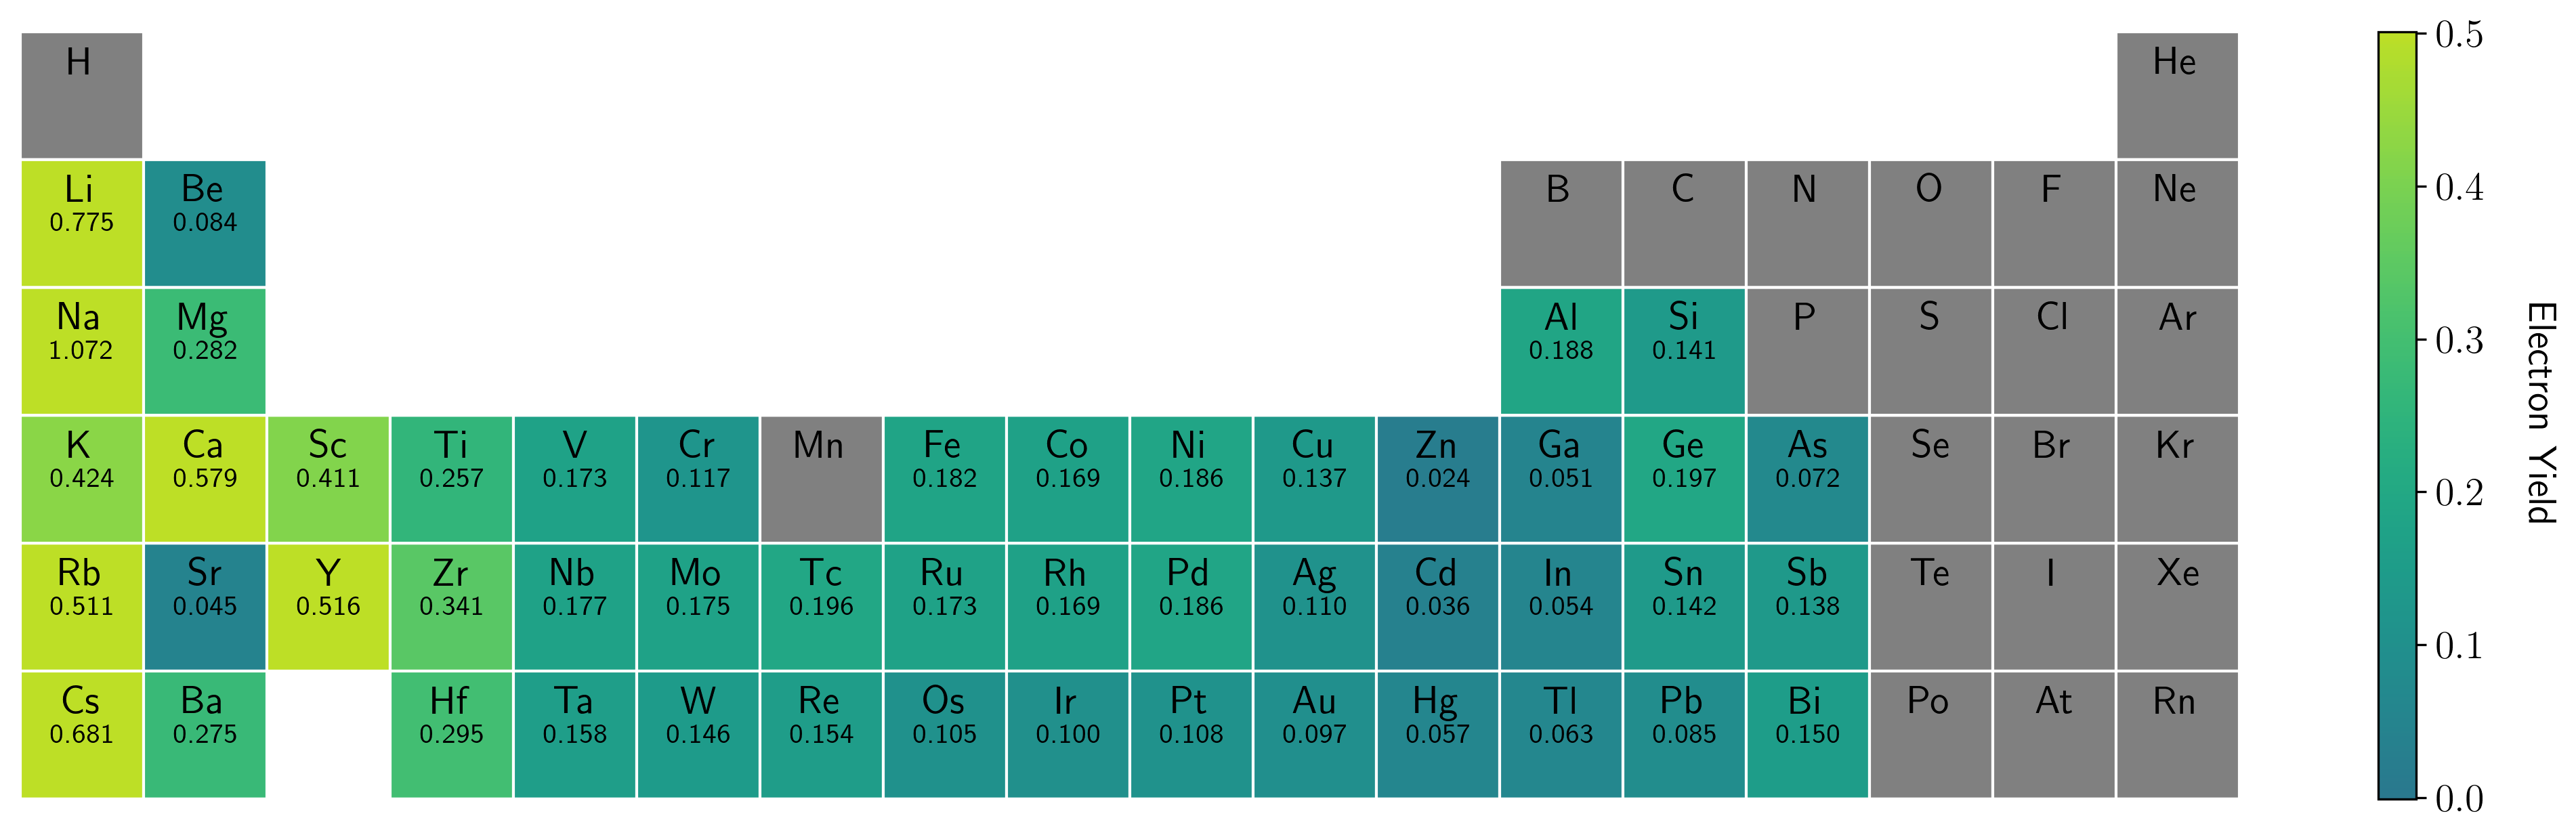
\includegraphics[width=\textwidth]{figures/quotas/He_yield_table.png} 
\caption{Average yield results for \ce{He+} ions on the surfaces of the 
studied elements.} 
\label{quotas:fig-He_yield_table} 
\end{figure} 

\begin{figure}[ht] 
\centering 
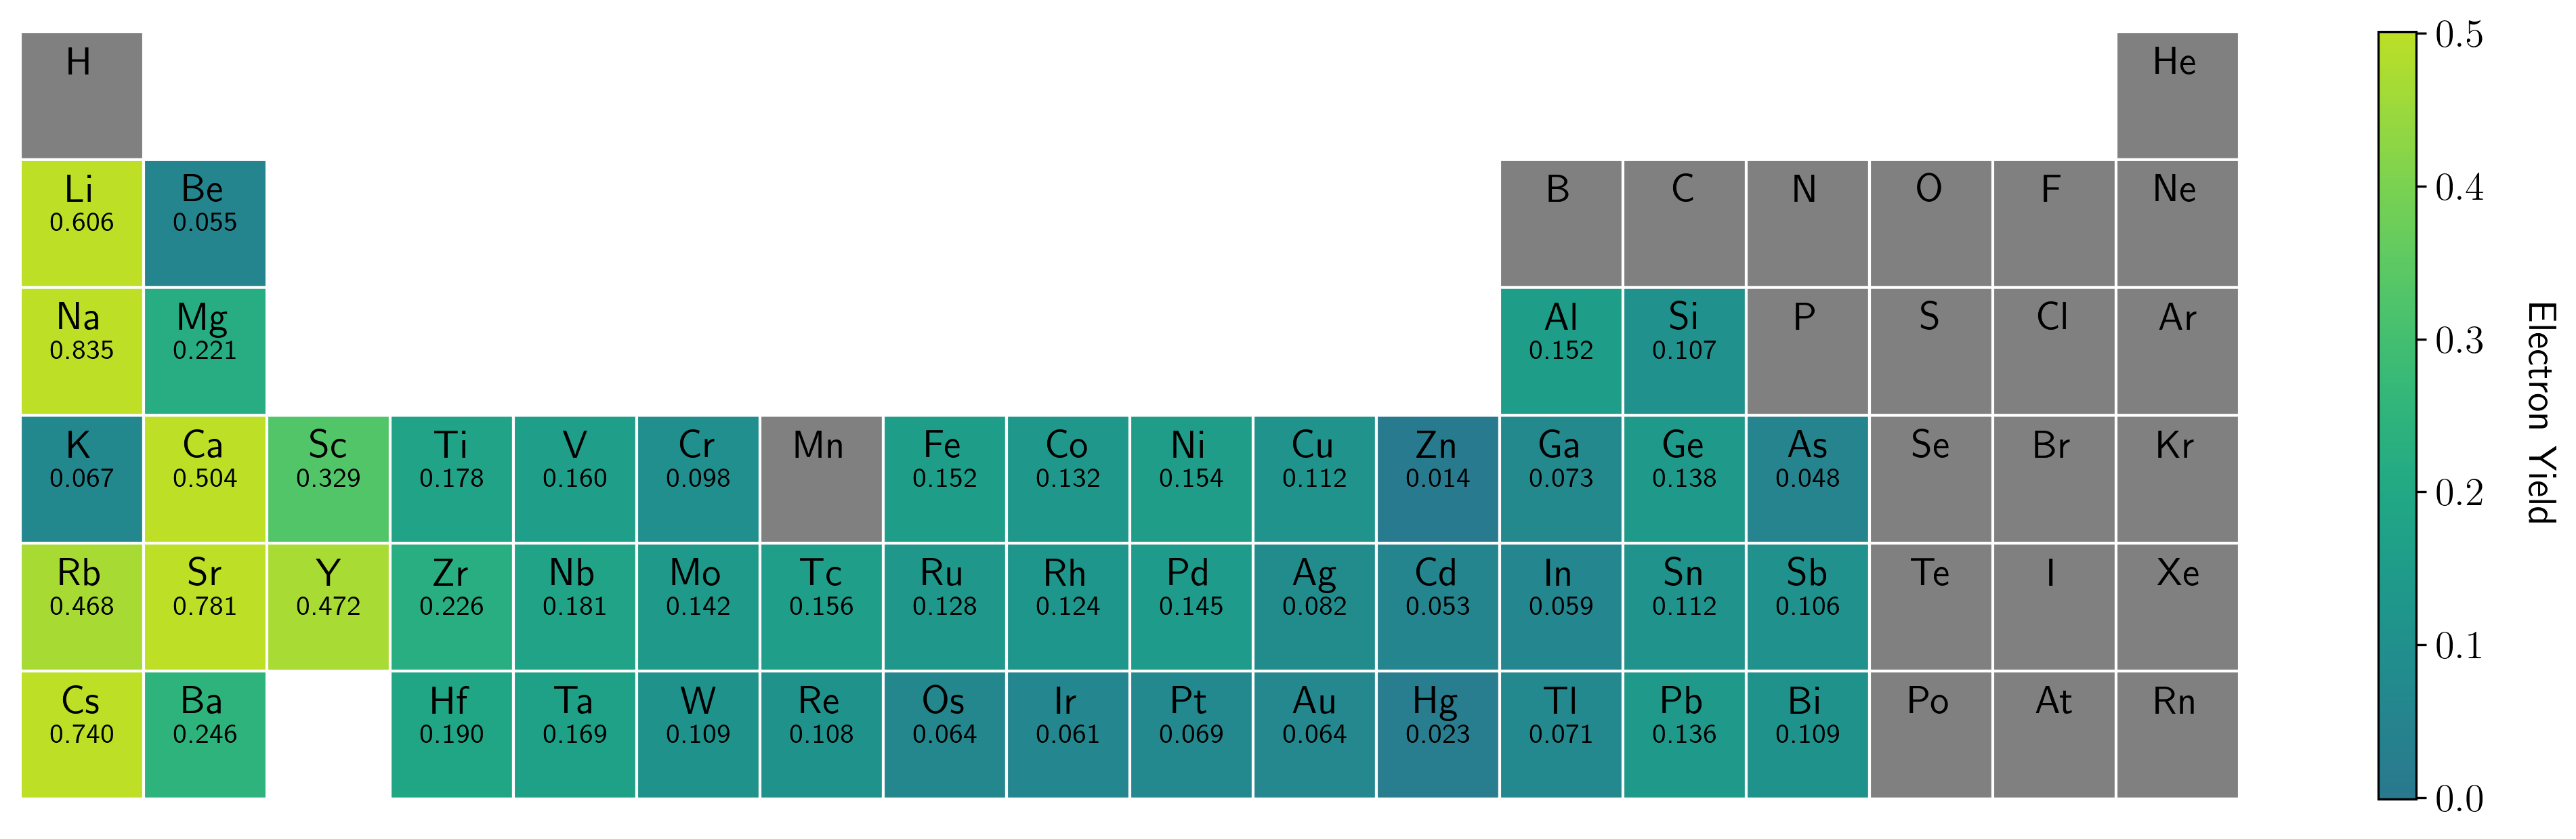
\includegraphics[width=\textwidth]{figures/quotas/Ne_yield_table.png} 
\caption{Average yield results for \ce{Ne+} ions on the surfaces of the 
studied elements.} 
\label{quotas:fig-Ne_yield_table} 
\end{figure} 

On the other side of the periodic table, elements with full $d$ orbitals and 
only a couple of electrons in the $s$ and/or $p$ orbitals (group 11-13, 
excluding \ce{Al}) have a noticeably lower yield. This is connected to the 
electronic structure of these elements near the Fermi level. Fig.~\ref{quotas:fig-pdos} 
shows the projected DOS of \ce{Ni (100)}, \ce{Cu (100)} and \ce{Zn (100)}. 
For all of these surfaces, most of the occupied states near the Fermi level 
correspond to $d$ states. However, for \ce{Zn (100)} these 
lie significantly below the Fermi level, which means that the average energy of electrons that 
participate in the Auger neutralization and electron scattering processes is 
relatively low. This reduces the average energy of the excited electron, 
which results in a lower chance of escape and hence a lower yield. The electronic  structures of 
other elements with full $d$ orbitals is similar, resulting in a lower yield 
for groups 11-13. \ce{Cu}, and by extension \ce{Ag} and \ce{Au}, suffer from a
similar effect, but to a lesser extent because the 
the $d$ states are closer to the Fermi level. Finally, this also explains the relatively low results for \ce{He+} ions on \ce{K}, \ce{Sr} and \ce{Ba}. 

{
\pgfplotsset{every axis/.style={font=\sffamily, width=6cm, height=7cm,
legend style={font=\footnotesize\sffamily,
fill opacity=0.8, text opacity=1}}} 
\begin{figure}[ht] 
    \begin{subfigure}[t]{0.33\textwidth} 
        \centering 
        % This file was created by tikzplotlib v0.8.7.
\begin{tikzpicture}

\definecolor{color0}{rgb}{0.894117647058824,0.101960784313725,0.109803921568627}
\definecolor{color1}{rgb}{0.215686274509804,0.494117647058824,0.72156862745098}
\definecolor{color2}{rgb}{0.301960784313725,0.686274509803922,0.290196078431373}

\node [font=\sffamily] at (1,5) {Ni (100)};

\begin{axis}[
legend cell align={left},
xlabel={Energy (eV)},
xmin=-20, xmax=20,
xtick style={draw=none},
xtick={-19,-10,0,10,19},
xticklabels={-20,-10,0,10,20},
ymin=0, ymax=30,
ylabel={DOS (a.u.)},
ylabel shift = -6 pt,
ytick style={},
ytick={}, 
yticklabels={}
]
\addplot [very thick, color0]
table {%
-70.69028876 0
-70.61898876 0
-70.54758876 0
-70.47618876 0
-70.40488876 0
-70.33348876 0
-70.26208876 0
-70.19068876 0
-70.11938876 0
-70.04798876 0
-69.97658876 0
-69.90528876 0
-69.83388876 0
-69.76248876 0
-69.69108876 0
-69.61978876 0
-69.54838876 0
-69.47698876 0
-69.40568876 0
-69.33428876 0
-69.26288876 0
-69.19158876 0
-69.12018876 0
-69.04878876 0
-68.97738876 0
-68.90608876 0
-68.83468876 0
-68.76328876 0
-68.69198876 0
-68.62058876 0
-68.54918876 0
-68.47778876 0
-68.40648876 0
-68.33508876 0
-68.26368876 0
-68.19238876 0
-68.12098876 0
-68.04958876 0
-67.97818876 0
-67.90688876 0
-67.83548876 0
-67.76408876 0
-67.69278876 0
-67.62138876 0
-67.54998876 0
-67.47868876 0
-67.40728876 0
-67.33588876 0
-67.26448876 0
-67.19318876 0
-67.12178876 0
-67.05038876 0
-66.97908876 0
-66.90768876 0
-66.83628876 0
-66.76488876 0
-66.69358876 0
-66.62218876 0
-66.55078876 0
-66.47948876 0
-66.40808876 0
-66.33668876 0
-66.26528876 0
-66.19398876 0
-66.12258876 0
-66.05118876 0
-65.97988876 0
-65.90848876 0
-65.83708876 0
-65.76578876 0
-65.69438876 0
-65.62298876 0
-65.55158876 0
-65.48028876 0
-65.40888876 0
-65.33748876 0
-65.26618876 0
-65.19478876 0
-65.12338876 0
-65.05198876 0
-64.98068876 0
-64.90928876 0
-64.83788876 0
-64.76658876 0
-64.69518876 0
-64.62378876 0
-64.55238876 0
-64.48108876 0
-64.40968876 0
-64.33828876 0
-64.26698876 0
-64.19558876 0
-64.12418876 0.0004
-64.05288876 0.0002
-63.98148876 0.0002
-63.91008876 0
-63.83868876 0
-63.76738876 0.0004
-63.69598876 0
-63.62458876 0
-63.55328876 0
-63.48188876 0
-63.41048876 0
-63.33908876 0
-63.26778876 0
-63.19638876 0.0001
-63.12498876 0.0001
-63.05368876 0
-62.98228876 0
-62.91088876 0
-62.83948876 0
-62.76818876 0
-62.69678876 0
-62.62538876 0
-62.55408876 0
-62.48268876 0
-62.41128876 0
-62.33998876 0
-62.26858876 0
-62.19718876 0
-62.12578876 0
-62.05448876 0
-61.98308876 0
-61.91168876 0
-61.84038876 0
-61.76898876 0
-61.69758876 0
-61.62618876 0
-61.55488876 0
-61.48348876 0
-61.41208876 0
-61.34078876 0
-61.26938876 0
-61.19798876 0
-61.12658876 0
-61.05528876 0
-60.98388876 0
-60.91248876 0
-60.84118876 0
-60.76978876 0
-60.69838876 0
-60.62708876 0
-60.55568876 0
-60.48428876 0
-60.41288876 0
-60.34158876 0
-60.27018876 0
-60.19878876 0
-60.12748876 0
-60.05608876 0
-59.98468876 0
-59.91328876 0
-59.84198876 0
-59.77058876 0
-59.69918876 0
-59.62788876 0
-59.55648876 0
-59.48508876 0
-59.41368876 0
-59.34238876 0
-59.27098876 0
-59.19958876 0
-59.12828876 0
-59.05688876 0
-58.98548876 0
-58.91418876 0
-58.84278876 0
-58.77138876 0
-58.69998876 0
-58.62868876 0
-58.55728876 0
-58.48588876 0
-58.41458876 0
-58.34318876 0
-58.27178876 0
-58.20038876 0
-58.12908876 0
-58.05768876 0
-57.98628876 0
-57.91498876 0
-57.84358876 0
-57.77218876 0
-57.70078876 0
-57.62948876 0
-57.55808876 0
-57.48668876 0
-57.41538876 0
-57.34398876 0
-57.27258876 0
-57.20128876 0
-57.12988876 0
-57.05848876 0
-56.98708876 0
-56.91578876 0
-56.84438876 0
-56.77298876 0
-56.70168876 0
-56.63028876 0
-56.55888876 0
-56.48748876 0
-56.41618876 0
-56.34478876 0
-56.27338876 0
-56.20208876 0
-56.13068876 0
-56.05928876 0
-55.98788876 0
-55.91658876 0
-55.84518876 0
-55.77378876 0
-55.70248876 0
-55.63108876 0
-55.55968876 0
-55.48838876 0
-55.41698876 0
-55.34558876 0
-55.27418876 0
-55.20288876 0
-55.13148876 0
-55.06008876 0
-54.98878876 0
-54.91738876 0
-54.84598876 0
-54.77458876 0
-54.70328876 0
-54.63188876 0
-54.56048876 0
-54.48918876 0
-54.41778876 0
-54.34638876 0
-54.27498876 0
-54.20368876 0
-54.13228876 0
-54.06088876 0
-53.98958876 0
-53.91818876 0
-53.84678876 0
-53.77548876 0
-53.70408876 0
-53.63268876 0
-53.56128876 0
-53.48998876 0
-53.41858876 0
-53.34718876 0
-53.27588876 0
-53.20448876 0
-53.13308876 0
-53.06168876 0
-52.99038876 0
-52.91898876 0
-52.84758876 0
-52.77628876 0
-52.70488876 0
-52.63348876 0
-52.56208876 0
-52.49078876 0
-52.41938876 0
-52.34798876 0
-52.27668876 0
-52.20528876 0
-52.13388876 0
-52.06258876 0
-51.99118876 0
-51.91978876 0
-51.84838876 0
-51.77708876 0
-51.70568876 0
-51.63428876 0
-51.56298876 0
-51.49158876 0
-51.42018876 0
-51.34878876 0
-51.27748876 0
-51.20608876 0
-51.13468876 0
-51.06338876 0
-50.99198876 0
-50.92058876 0
-50.84918876 0
-50.77788876 0
-50.70648876 0
-50.63508876 0
-50.56378876 0
-50.49238876 0
-50.42098876 0
-50.34968876 0
-50.27828876 0
-50.20688876 0
-50.13548876 0
-50.06418876 0
-49.99278876 0
-49.92138876 0
-49.85008876 0
-49.77868876 0
-49.70728876 0
-49.63588876 0
-49.56458876 0
-49.49318876 0
-49.42178876 0
-49.35048876 0
-49.27908876 0
-49.20768876 0
-49.13628876 0
-49.06498876 0
-48.99358876 0
-48.92218876 0
-48.85088876 0
-48.77948876 0
-48.70808876 0
-48.63678876 0
-48.56538876 0
-48.49398876 0
-48.42258876 0
-48.35128876 0
-48.27988876 0
-48.20848876 0
-48.13718876 0
-48.06578876 0
-47.99438876 0
-47.92298876 0
-47.85168876 0
-47.78028876 0
-47.70888876 0
-47.63758876 0
-47.56618876 0
-47.49478876 0
-47.42338876 0
-47.35208876 0
-47.28068876 0
-47.20928876 0
-47.13798876 0
-47.06658876 0
-46.99518876 0
-46.92388876 0
-46.85248876 0
-46.78108876 0
-46.70968876 0
-46.63838876 0
-46.56698876 0
-46.49558876 0
-46.42428876 0
-46.35288876 0
-46.28148876 0
-46.21008876 0
-46.13878876 0
-46.06738876 0
-45.99598876 0
-45.92468876 0
-45.85328876 0
-45.78188876 0
-45.71048876 0
-45.63918876 0
-45.56778876 0
-45.49638876 0
-45.42508876 0
-45.35368876 0
-45.28228876 0
-45.21098876 0
-45.13958876 0
-45.06818876 0
-44.99678876 0
-44.92548876 0
-44.85408876 0
-44.78268876 0
-44.71138876 0
-44.63998876 0
-44.56858876 0
-44.49718876 0
-44.42588876 0
-44.35448876 0
-44.28308876 0
-44.21178876 0
-44.14038876 0
-44.06898876 0
-43.99758876 0
-43.92628876 0
-43.85488876 0
-43.78348876 0
-43.71218876 0
-43.64078876 0
-43.56938876 0
-43.49798876 0
-43.42668876 0
-43.35528876 0
-43.28388876 0
-43.21258876 0
-43.14118876 0
-43.06978876 0
-42.99848876 0
-42.92708876 0
-42.85568876 0
-42.78428876 0
-42.71298876 0
-42.64158876 0
-42.57018876 0
-42.49888876 0
-42.42748876 0
-42.35608876 0
-42.28468876 0
-42.21338876 0
-42.14198876 0
-42.07058876 0
-41.99928876 0
-41.92788876 0
-41.85648876 0
-41.78508876 0
-41.71378876 0
-41.64238876 0
-41.57098876 0
-41.49968876 0
-41.42828876 0
-41.35688876 0
-41.28558876 0
-41.21418876 0
-41.14278876 0
-41.07138876 0
-41.00008876 0
-40.92868876 0
-40.85728876 0
-40.78598876 0
-40.71458876 0
-40.64318876 0
-40.57178876 0
-40.50048876 0
-40.42908876 0
-40.35768876 0
-40.28638876 0
-40.21498876 0
-40.14358876 0
-40.07218876 0
-40.00088876 0
-39.92948876 0
-39.85808876 0
-39.78678876 0
-39.71538876 0
-39.64398876 0
-39.57268876 0
-39.50128876 0
-39.42988876 0
-39.35848876 0
-39.28718876 0
-39.21578876 0
-39.14438876 0
-39.07308876 0
-39.00168876 0
-38.93028876 0
-38.85888876 0
-38.78758876 0
-38.71618876 0
-38.64478876 0
-38.57348876 0
-38.50208876 0
-38.43068876 0
-38.35928876 0
-38.28798876 0
-38.21658876 0
-38.14518876 0
-38.07388876 0
-38.00248876 0
-37.93108876 0
-37.85978876 0
-37.78838876 0
-37.71698876 0
-37.64558876 0
-37.57428876 0
-37.50288876 0
-37.43148876 0
-37.36018876 0
-37.28878876 0
-37.21738876 0
-37.14598876 0
-37.07468876 0
-37.00328876 0
-36.93188876 0
-36.86058876 0
-36.78918876 0
-36.71778876 0
-36.64638876 0
-36.57508876 0
-36.50368876 0
-36.43228876 0
-36.36098876 0
-36.28958876 0
-36.21818876 0
-36.14688876 0
-36.07548876 0
-36.00408876 0
-35.93268876 0
-35.86138876 0
-35.78998876 0
-35.71858876 0
-35.64728876 0
-35.57588876 0
-35.50448876 0
-35.43308876 0
-35.36178876 0
-35.29038876 0
-35.21898876 0
-35.14768876 0
-35.07628876 0
-35.00488876 0
-34.93348876 0
-34.86218876 0
-34.79078876 0
-34.71938876 0
-34.64808876 0
-34.57668876 0
-34.50528876 0
-34.43398876 0
-34.36258876 0
-34.29118876 0
-34.21978876 0
-34.14848876 0
-34.07708876 0
-34.00568876 0
-33.93438876 0
-33.86298876 0
-33.79158876 0
-33.72018876 0
-33.64888876 0
-33.57748876 0
-33.50608876 0
-33.43478876 0
-33.36338876 0
-33.29198876 0
-33.22058876 0
-33.14928876 0
-33.07788876 0
-33.00648876 0
-32.93518876 0
-32.86378876 0
-32.79238876 0
-32.72108876 0
-32.64968876 0
-32.57828876 0
-32.50688876 0
-32.43558876 0
-32.36418876 0
-32.29278876 0
-32.22148876 0
-32.15008876 0
-32.07868876 0
-32.00728876 0
-31.93598876 0
-31.86458876 0
-31.79318876 0
-31.72188876 0
-31.65048876 0
-31.57908876 0
-31.50768876 0
-31.43638876 0
-31.36498876 0
-31.29358876 0
-31.22228876 0
-31.15088876 0
-31.07948876 0
-31.00818876 0
-30.93678876 0
-30.86538876 0
-30.79398876 0
-30.72268876 0
-30.65128876 0
-30.57988876 0
-30.50858876 0
-30.43718876 0
-30.36578876 0
-30.29438876 0
-30.22308876 0
-30.15168876 0
-30.08028876 0
-30.00898876 0
-29.93758876 0
-29.86618876 0
-29.79478876 0
-29.72348876 0
-29.65208876 0
-29.58068876 0
-29.50938876 0
-29.43798876 0
-29.36658876 0
-29.29528876 0
-29.22388876 0
-29.15248876 0
-29.08108876 0
-29.00978876 0
-28.93838876 0
-28.86698876 0
-28.79568876 0
-28.72428876 0
-28.65288876 0
-28.58148876 0
-28.51018876 0
-28.43878876 0
-28.36738876 0
-28.29608876 0
-28.22468876 0
-28.15328876 0
-28.08188876 0
-28.01058876 0
-27.93918876 0
-27.86778876 0
-27.79648876 0
-27.72508876 0
-27.65368876 0
-27.58238876 0
-27.51098876 0
-27.43958876 0
-27.36818876 0
-27.29688876 0
-27.22548876 0
-27.15408876 0
-27.08278876 0
-27.01138876 0
-26.93998876 0
-26.86858876 0
-26.79728876 0
-26.72588876 0
-26.65448876 0
-26.58318876 0
-26.51178876 0
-26.44038876 0
-26.36898876 0
-26.29768876 0
-26.22628876 0
-26.15488876 0
-26.08358876 0
-26.01218876 0
-25.94078876 0
-25.86948876 0
-25.79808876 0
-25.72668876 0
-25.65528876 0
-25.58398876 0
-25.51258876 0
-25.44118876 0
-25.36988876 0
-25.29848876 0
-25.22708876 0
-25.15568876 0
-25.08438876 0
-25.01298876 0
-24.94158876 0
-24.87028876 0
-24.79888876 0
-24.72748876 0
-24.65608876 0
-24.58478876 0
-24.51338876 0
-24.44198876 0
-24.37068876 0
-24.29928876 0
-24.22788876 0
-24.15658876 0
-24.08518876 0
-24.01378876 0
-23.94238876 0
-23.87108876 0
-23.79968876 0
-23.72828876 0
-23.65698876 0
-23.58558876 0
-23.51418876 0
-23.44278876 0
-23.37148876 0
-23.30008876 0
-23.22868876 0
-23.15738876 0
-23.08598876 0
-23.01458876 0
-22.94318876 0
-22.87188876 0
-22.80048876 0
-22.72908876 0
-22.65778876 0
-22.58638876 0
-22.51498876 0
-22.44368876 0
-22.37228876 0
-22.30088876 0
-22.22948876 0
-22.15818876 0
-22.08678876 0
-22.01538876 0
-21.94408876 0
-21.87268876 0
-21.80128876 0
-21.72988876 0
-21.65858876 0
-21.58718876 0
-21.51578876 0
-21.44448876 0
-21.37308876 0
-21.30168876 0
-21.23028876 0
-21.15898876 0
-21.08758876 0
-21.01618876 0
-20.94488876 0
-20.87348876 0
-20.80208876 0
-20.73078876 0
-20.65938876 0
-20.58798876 0
-20.51658876 0
-20.44528876 0
-20.37388876 0
-20.30248876 0
-20.23118876 0
-20.15978876 0
-20.08838876 0
-20.01698876 0
-19.94568876 0
-19.87428876 0
-19.80288876 0
-19.73158876 0
-19.66018876 0
-19.58878876 0
-19.51738876 0
-19.44608876 0
-19.37468876 0
-19.30328876 0
-19.23198876 0
-19.16058876 0
-19.08918876 0
-19.01788876 0
-18.94648876 0
-18.87508876 0
-18.80368876 0
-18.73238876 0
-18.66098876 0
-18.58958876 0
-18.51828876 0
-18.44688876 0
-18.37548876 0
-18.30408876 0
-18.23278876 0
-18.16138876 0
-18.08998876 0
-18.01868876 0
-17.94728876 0
-17.87588876 0
-17.80448876 0
-17.73318876 0
-17.66178876 0
-17.59038876 0
-17.51908876 0
-17.44768876 0
-17.37628876 0
-17.30498876 0
-17.23358876 0
-17.16218876 0
-17.09078876 0
-17.01948876 0
-16.94808876 0
-16.87668876 0
-16.80538876 0
-16.73398876 0
-16.66258876 0
-16.59118876 0
-16.51988876 0
-16.44848876 0
-16.37708876 0
-16.30578876 0
-16.23438876 0
-16.16298876 0
-16.09158876 0
-16.02028876 0
-15.94888876 0
-15.87748876 0
-15.80618876 0
-15.73478876 0
-15.66338876 0
-15.59208876 0
-15.52068876 0
-15.44928876 0
-15.37788876 0
-15.30658876 0
-15.23518876 0
-15.16378876 0
-15.09248876 0
-15.02108876 0
-14.94968876 0
-14.87828876 0
-14.80698876 0
-14.73558876 0
-14.66418876 0
-14.59288876 0
-14.52148876 0
-14.45008876 0
-14.37868876 0
-14.30738876 0
-14.23598876 0
-14.16458876 0
-14.09328876 0
-14.02188876 0
-13.95048876 0
-13.87918876 0
-13.80778876 0
-13.73638876 0
-13.66498876 0
-13.59368876 0
-13.52228876 0
-13.45088876 0
-13.37958876 0
-13.30818876 0
-13.23678876 0
-13.16538876 0
-13.09408876 0
-13.02268876 0
-12.95128876 0
-12.87998876 0
-12.80858876 0
-12.73718876 0
-12.66578876 0
-12.59448876 0
-12.52308876 0
-12.45168876 0
-12.38038876 0
-12.30898876 0
-12.23758876 0
-12.16628876 0
-12.09488876 0
-12.02348876 0
-11.95208876 0
-11.88078876 0
-11.80938876 0
-11.73798876 0
-11.66668876 0
-11.59528876 0
-11.52388876 0
-11.45248876 0
-11.38118876 0
-11.30978876 0
-11.23838876 0
-11.16708876 0
-11.09568876 0
-11.02428876 0
-10.95288876 0
-10.88158876 0
-10.81018876 0
-10.73878876 0
-10.66748876 0
-10.59608876 0
-10.52468876 0
-10.45338876 0
-10.38198876 0
-10.31058876 0
-10.23918876 0
-10.16788876 0
-10.09648876 0
-10.02508876 0
-9.95378876 0
-9.88238876 0
-9.81098876 0
-9.73958876 0
-9.66828876 0
-9.59688876 0
-9.52548876 0
-9.45418876 0
-9.38278876 0
-9.31138876 0
-9.23998876 0
-9.16868876 0
-9.09728876 0
-9.02588876 0
-8.95458876 0
-8.88318876 0
-8.81178876 0
-8.74038876 0
-8.66908876 0
-8.59768876 0
-8.52628876 0
-8.45498876 0
-8.38358876 0
-8.31218876 0
-8.24088876 0.0002
-8.16948876 0.0002
-8.09808876 0.0004
-8.02668876 0.0006
-7.95538876 0.001
-7.88398876 0.0025
-7.81258876 0.0025
-7.74128876 0.0038
-7.66988876 0.0045
-7.59848876 0.0051
-7.52708876 0.0054
-7.45578876 0.0066
-7.38438876 0.0069
-7.31298876 0.0101
-7.24168876 0.0111
-7.17028876 0.0132
-7.09888876 0.0146
-7.02748876 0.0175
-6.95618876 0.0164
-6.88478876 0.0204
-6.81338876 0.0239
-6.74208876 0.0226
-6.67068876 0.0299
-6.59928876 0.0363
-6.52798876 0.0363
-6.45658876 0.0456
-6.38518876 0.0478
-6.31378876 0.0499
-6.24248876 0.0588
-6.17108876 0.0671
-6.09968876 0.069
-6.02838876 0.0759
-5.95698876 0.0942
-5.88558876 0.1104
-5.81418876 0.119
-5.74288876 0.127
-5.67148876 0.1606
-5.60008876 0.1602
-5.52878876 0.1719
-5.45738876 0.2203
-5.38598876 0.2277
-5.31458876 0.2674
-5.24328876 0.3238
-5.17188876 0.3812
-5.10048876 0.4294
-5.02918876 0.498
-4.95778876 0.6017
-4.88638876 0.7326
-4.81508876 0.9724
-4.74368876 1.4087
-4.67228876 1.5977
-4.60088876 1.6963
-4.52958876 2.243
-4.45818876 3.3095
-4.38678876 3.6974
-4.31548876 3.3944
-4.24408876 3.475
-4.17268876 4.0566
-4.10128876 4.9936
-4.02998876 6.4818
-3.95858876 7.1538
-3.88718876 7.5937
-3.81588876 7.8529
-3.74448876 8.0061
-3.67308876 9.2839
-3.60168876 9.7164
-3.53038876 8.2759
-3.45898876 7.1998
-3.38758876 7.1242
-3.31628876 7.5269
-3.24488876 8.1236
-3.17348876 8.939
-3.10218876 10.1902
-3.03078876 10.1228
-2.95938876 9.8898
-2.88798876 9.4829
-2.81668876 10.3681
-2.74528876 10.1678
-2.67388876 10.3689
-2.60258876 10.7039
-2.53118876 12.2262
-2.45978876 13.9936
-2.38838876 15.8885
-2.31708876 16.665
-2.24568876 16.7592
-2.17428876 17.5754
-2.10298876 14.096
-2.03158876 15.4209
-1.96018876 14.5619
-1.88878876 15.4133
-1.81748876 14.0197
-1.74608876 12.6824
-1.67468876 13.126
-1.60338876 14.7622
-1.53198876 15.04
-1.46058876 15.839
-1.38928876 15.2835
-1.31788876 16.2132
-1.24648876 17.8321
-1.17508876 17.0194
-1.10378876 17.3039
-1.03238876 16.9406
-0.96098876 17.3542
-0.88968876 17.5953
-0.81828876 18.7969
-0.74688876 21.7522
-0.67548876 23.6618
-0.60418876 22.9732
-0.53278876 16.5773
-0.46138876 11.4343
-0.39008876 8.9115
-0.31868876 8.9348
-0.24728876 9.1059
-0.17588876 8.4842
-0.10458876 7.2722
-0.03318876 6.5911
0.0382112399999999 6.3129
0.10951124 6.8382
0.18091124 7.3951
0.25231124 4.3732
0.32361124 2.5176
0.39501124 2.1191
0.46641124 1.8508
0.53781124 1.549
0.60911124 1.3569
0.68051124 1.4738
0.75191124 1.3135
0.82321124 1.3583
0.89461124 1.2079
0.96601124 1.1536
1.03741124 1.1295
1.10871124 1.1195
1.18011124 1.0737
1.25151124 0.9983
1.32281124 1.0443
1.39421124 1.0208
1.46561124 0.8732
1.53701124 1.0314
1.60831124 0.9776
1.67971124 0.7982
1.75111124 0.8387
1.82241124 0.8639
1.89381124 0.8156
1.96521124 0.7712
2.03651124 0.7835
2.10791124 0.6474
2.17931124 0.7955
2.25071124 0.7626
2.32201124 0.6666
2.39341124 0.7664
2.46481124 0.6462
2.53611124 0.6323
2.60751124 0.6617
2.67891124 0.6709
2.75031124 0.5746
2.82161124 0.5025
2.89301124 0.638
2.96441124 0.602
3.03571124 0.4745
3.10711124 0.5591
3.17851124 0.5854
3.24991124 0.5221
3.32121124 0.5326
3.39261124 0.4603
3.46401124 0.4867
3.53531124 0.5189
3.60671124 0.4376
3.67811124 0.3833
3.74941124 0.4482
3.82081124 0.4312
3.89221124 0.4041
3.96361124 0.3862
4.03491124 0.4169
4.10631124 0.3826
4.17771124 0.3561
4.24901124 0.3404
4.32041124 0.4016
4.39181124 0.3038
4.46321124 0.3575
4.53451124 0.3209
4.60591124 0.3713
4.67731124 0.3797
4.74861124 0.4403
4.82001124 0.3574
4.89141124 0.3684
4.96281124 0.376
5.03411124 0.354
5.10551124 0.3833
5.17691124 0.3242
5.24821124 0.3294
5.31961124 0.3059
5.39101124 0.3098
5.46231124 0.3212
5.53371124 0.2871
5.60511124 0.2851
5.67651124 0.2595
5.74781124 0.2665
5.81921124 0.2794
5.89061124 0.2278
5.96191124 0.252
6.03331124 0.484
6.10471124 0.5829
6.17611124 0.5544
6.24741124 0.4899
6.31881124 0.5587
6.39021124 0.5734
6.46151124 0.5892
6.53291124 0.6514
6.60431124 0.61
6.67571124 0.6066
6.74701124 0.5779
6.81841124 0.4986
6.88981124 0.4337
6.96111124 0.4591
7.03251124 0.4682
7.10391124 0.4138
7.17521124 0.378
7.24661124 0.4015
7.31801124 0.4243
7.38941124 0.4655
7.46071124 0.5548
7.53211124 0.5408
7.60351124 0.4839
7.67481124 0.4559
7.74621124 0.3922
7.81761124 0.3586
7.88901124 0.3551
7.96031124 0.3521
8.03171124 0.3627
8.10311124 0.3981
8.17441124 0.4862
8.24581124 0.3832
8.31721124 0.3395
8.38861124 0.347
8.45991124 0.3636
8.53131124 0.4078
8.60271124 0.4081
8.67401124 0.394
8.74541124 0.3889
8.81681124 0.3551
8.88811124 0.3341
8.95951124 0.3325
9.03091124 0.3383
9.10231124 0.3618
9.17361124 0.4201
9.24501124 0.4638
9.31641124 0.4679
9.38771124 0.4655
9.45911124 0.4932
9.53051124 0.4897
9.60191124 0.4811
9.67321124 0.4372
9.74461124 0.4372
9.81601124 0.4825
9.88731124 0.5016
9.95871124 0.5197
10.03011124 0.5509
10.10151124 0.5815
10.17281124 0.6192
10.24421124 0.5732
10.31561124 0.5175
10.38691124 0.5412
10.45831124 0.5815
10.52971124 0.5978
10.60101124 0.5419
10.67241124 0.5225
10.74381124 0.4847
10.81521124 0.4759
10.88651124 0.5381
10.95791124 0.5745
11.02931124 0.5239
11.10061124 0.4828
11.17201124 0.4883
11.24341124 0.5145
11.31481124 0.5428
11.38611124 0.5339
11.45751124 0.4863
11.52891124 0.5203
11.60021124 0.5623
11.67161124 0.5068
11.74301124 0.4284
11.81441124 0.4661
11.88571124 0.5473
11.95711124 0.5487
12.02851124 0.4937
12.09981124 0.513
12.17121124 0.5289
12.24261124 0.4675
12.31391124 0.4705
12.38531124 0.5052
12.45671124 0.4732
12.52811124 0.4796
12.59941124 0.4846
12.67081124 0.4871
12.74221124 0.5087
12.81351124 0.4734
12.88491124 0.4716
12.95631124 0.4419
13.02771124 0.4264
13.09901124 0.4754
13.17041124 0.4387
13.24181124 0.4843
13.31311124 0.5057
13.38451124 0.498
13.45591124 0.4941
13.52731124 0.4707
13.59861124 0.5268
13.67001124 0.5155
13.74141124 0.4291
13.81271124 0.4469
13.88411124 0.4929
13.95551124 0.4734
14.02681124 0.5233
14.09821124 0.5041
14.16961124 0.4733
14.24101124 0.4657
14.31231124 0.4543
14.38371124 0.4526
14.45511124 0.4548
14.52641124 0.4724
14.59781124 0.4292
14.66921124 0.4973
14.74061124 0.4472
14.81191124 0.4812
14.88331124 0.4773
14.95471124 0.4285
15.02601124 0.4313
15.09741124 0.4758
15.16881124 0.4851
15.24021124 0.4797
15.31151124 0.4127
15.38291124 0.4699
15.45431124 0.4373
15.52561124 0.5264
15.59701124 0.5188
15.66841124 0.461
15.73971124 0.4753
15.81111124 0.4569
15.88251124 0.47
15.95391124 0.4465
16.02521124 0.458
16.09661124 0.5011
16.16801124 0.5079
16.23931124 0.4793
16.31071124 0.4594
16.38211124 0.3766
16.45351124 0.4055
16.52481124 0.5363
16.59621124 0.5067
16.66761124 0.4599
16.73891124 0.4178
16.81031124 0.4123
16.88171124 0.4246
16.95311124 0.4917
17.02441124 0.4897
17.09581124 0.4324
17.16721124 0.4501
17.23851124 0.4228
17.30991124 0.4332
17.38131124 0.4408
17.45261124 0.437
17.52401124 0.436
17.59541124 0.4852
17.66681124 0.4634
17.73811124 0.4201
17.80951124 0.4543
17.88091124 0.4622
17.95221124 0.4876
18.02361124 0.4381
18.09501124 0.4071
18.16641124 0.4519
18.23771124 0.4863
18.30911124 0.4776
18.38051124 0.4597
18.45181124 0.4343
18.52321124 0.4223
18.59461124 0.3863
18.66601124 0.4787
18.73731124 0.4557
18.80871124 0.4314
18.88011124 0.4404
18.95141124 0.3985
19.02281124 0.4255
19.09421124 0.4263
19.16551124 0.4555
19.23691124 0.4449
19.30831124 0.4306
19.37971124 0.4213
19.45101124 0.431
19.52241124 0.4558
19.59381124 0.4475
19.66511124 0.4184
19.73651124 0.4379
19.80791124 0.4342
19.87931124 0.4337
19.95061124 0.5153
20.02201124 0.4514
20.09341124 0.4638
20.16471124 0.5407
20.23611124 0.5981
20.30751124 0.5369
20.37891124 0.5205
20.45021124 0.5783
20.52161124 0.6482
20.59301124 0.5824
20.66431124 0.5182
20.73571124 0.5549
20.80711124 0.6069
20.87841124 0.6059
20.94981124 0.6426
21.02121124 0.6923
21.09261124 0.6248
21.16391124 0.6665
21.23531124 0.6533
21.30671124 0.6775
21.37801124 0.6603
21.44941124 0.6976
21.52081124 0.7733
21.59221124 0.7574
21.66351124 0.67
21.73491124 0.7177
21.80631124 0.7627
21.87761124 0.6743
21.94901124 0.7264
22.02041124 0.7554
22.09181124 0.7261
22.16311124 0.7438
22.23451124 0.7494
22.30591124 0.7089
22.37721124 0.6962
22.44861124 0.6565
22.52001124 0.6905
22.59131124 0.7077
22.66271124 0.6705
22.73411124 0.7016
22.80551124 0.7086
22.87681124 0.6827
22.94821124 0.6947
23.01961124 0.6721
23.09091124 0.6376
23.16231124 0.6232
23.23371124 0.5604
23.30511124 0.6612
23.37641124 0.5634
23.44781124 0.6003
23.51921124 0.5836
23.59051124 0.6567
23.66191124 0.6949
23.73331124 0.5993
23.80471124 0.623
23.87601124 0.5511
23.94741124 0.5589
24.01881124 0.5816
24.09011124 0.579
24.16151124 0.5683
24.23291124 0.6135
24.30421124 0.5828
24.37561124 0.5591
24.44701124 0.5208
24.51841124 0.5026
24.58971124 0.5395
24.66111124 0.5723
24.73251124 0.5278
24.80381124 0.5155
24.87521124 0.5427
24.94661124 0.4965
25.01801124 0.5287
25.08931124 0.5844
25.16071124 0.498
25.23211124 0.5239
25.30341124 0.5391
25.37481124 0.4925
25.44621124 0.5064
25.51761124 0.4776
25.58891124 0.4715
25.66031124 0.4922
25.73171124 0.4998
25.80301124 0.5127
25.87441124 0.4451
25.94581124 0.4095
26.01721124 0.455
26.08851124 0.4666
26.15991124 0.4228
26.23131124 0.4117
26.30261124 0.4383
26.37401124 0.4286
26.44541124 0.3957
26.51671124 0.3899
26.58811124 0.4109
26.65951124 0.4413
26.73091124 0.4476
26.80221124 0.4683
26.87361124 0.4552
26.94501124 0.445
27.01631124 0.4631
27.08771124 0.4527
27.15911124 0.393
27.23051124 0.4386
27.30181124 0.4725
27.37321124 0.4285
27.44461124 0.429
27.51591124 0.4485
27.58731124 0.4178
27.65871124 0.4567
27.73011124 0.5075
27.80141124 0.5174
27.87281124 0.581
27.94421124 0.528
28.01551124 0.4993
28.08691124 0.6328
28.15831124 0.6172
28.22961124 0.6015
28.30101124 0.6364
28.37241124 0.5901
28.44381124 0.5396
28.51511124 0.6657
28.58651124 0.7734
28.65791124 0.6955
28.72921124 0.7635
28.80061124 0.7404
28.87201124 0.7126
28.94341124 0.8179
29.01471124 0.8147
29.08611124 0.9504
29.15751124 0.9191
29.22881124 0.9791
29.30021124 0.9838
29.37161124 1.0215
29.44301124 1.0803
29.51431124 1.0877
29.58571124 1.1653
29.65711124 1.1247
29.72841124 1.1835
29.79981124 1.0784
29.87121124 0.9973
29.94251124 0.9953
30.01391124 1.0099
30.08531124 1.0566
30.15671124 1.1026
30.22801124 1.0455
30.29941124 1.0398
30.37081124 0.9777
30.44211124 1.0368
30.51351124 1.0132
30.58491124 0.9811
30.65631124 0.9727
30.72761124 0.92
30.79901124 0.9719
30.87041124 1.0347
30.94171124 0.893099999999999
31.01311124 0.9232
31.08451124 0.9848
31.15591124 0.9915
31.22721124 0.8733
31.29861124 0.8851
31.37001124 0.9348
31.44131124 0.8103
31.51271124 0.8078
31.58411124 0.7837
31.65541124 0.825
31.72681124 0.852
31.79821124 0.9002
31.86961124 0.84
31.94091124 0.8263
32.01231124 0.8916
32.08371124 0.9994
32.15501124 0.8582
32.22641124 0.8782
32.29781124 0.8898
32.36921124 0.779
32.44051124 0.8274
32.51191124 0.9273
32.58331124 0.8797
32.65461124 0.8645
32.72601124 0.9524
32.79741124 0.873
32.86881124 0.8199
32.94011124 0.8318
33.01151124 0.927
33.08291124 1.08
33.15421124 0.9944
33.22561124 0.8825
33.29701124 1.0014
33.36831124 0.9706
33.43971124 1.0666
33.51111124 1.0906
33.58251124 1.1662
33.65381124 1.0783
33.72521124 1.0781
33.79661124 1.1063
33.86791124 1.0947
33.93931124 1.1142
34.01071124 1.1032
34.08211124 1.0768
34.15341124 1.2285
34.22481124 1.1149
34.29621124 1.0228
34.36751124 1.1252
34.43891124 1.0839
34.51031124 1.0796
34.58171124 1.1205
34.65301124 1.0917
34.72441124 1.0618
34.79581124 1.024
34.86711124 1.0705
34.93851124 1.0037
35.00991124 1.0175
35.08121124 1.0161
35.15261124 1.0463
35.22401124 1.097
35.29541124 1.0732
35.36671124 1.0085
35.43811124 0.9311
35.50951124 1.0144
35.58081124 0.9344
35.65221124 1.0163
35.72361124 1.0901
35.79501124 1.0695
35.86631124 0.9371
35.93771124 0.9541
36.00911124 0.9881
36.08041124 0.9513
36.15181124 0.9776
36.22321124 0.9749
36.29461124 0.9341
36.36591124 0.9971
36.43731124 0.951
36.50871124 0.9129
36.58001124 0.883
36.65141124 1.0191
36.72281124 0.9971
36.79411124 0.9237
36.86551124 0.927
36.93691124 0.9809
37.00831124 0.9518
37.07961124 0.9844
37.15101124 1.0775
37.22241124 1.1241
37.29371124 1.0918
37.36511124 1.0112
37.43651124 1.0403
37.50791124 0.9463
37.57921124 0.9453
37.65061124 0.9691
37.72201124 1.0149
37.79331124 1.0087
37.86471124 0.9471
37.93611124 0.9162
38.00751124 0.872
38.07881124 0.9548
38.15021124 1.0256
38.22161124 1.0609
38.29291124 1.1557
38.36431124 1.0535
38.43571124 1.0305
38.50701124 1.0223
38.57841124 1.0811
38.64981124 1.0325
38.72121124 0.9625
38.79251124 1.0032
38.86391124 1.0706
38.93531124 1.1082
39.00661124 1.06
39.07801124 1.0528
39.14941124 1.0826
39.22081124 1.075
39.29211124 1.1393
39.36351124 1.2094
39.43491124 1.1776
39.50621124 1.1125
39.57761124 1.1231
39.64901124 1.1676
39.72041124 1.1742
39.79171124 1.2274
39.86311124 1.2283
39.93451124 1.1314
40.00581124 1.1449
40.07721124 1.1262
40.14861124 1.1782
40.21991124 1.203
40.29131124 1.1772
40.36271124 1.1439
40.43411124 1.1568
40.50541124 1.1221
40.57681124 1.1758
40.64821124 1.2163
40.71951124 1.1194
40.79091124 1.1997
40.86231124 1.236
40.93371124 1.2365
41.00501124 1.2265
41.07641124 1.2237
41.14781124 1.1214
41.21911124 1.1956
41.29051124 1.1959
41.36191124 1.224
41.43331124 1.1989
41.50461124 1.1769
41.57601124 1.2275
41.64741124 1.1937
41.71871124 1.202
41.79011124 1.1407
41.86151124 1.0984
41.93281124 1.0483
42.00421124 1.1319
42.07561124 1.2414
42.14701124 1.1453
42.21831124 1.2195
42.28971124 1.3169
42.36111124 1.2164
42.43241124 1.181
42.50381124 1.2346
42.57521124 1.1278
42.64661124 1.2681
42.71791124 1.0927
42.78931124 1.0833
42.86071124 1.2603
42.93201124 1.2901
43.00341124 1.3161
43.07481124 1.295
43.14621124 1.2794
43.21751124 1.3254
43.28891124 1.4294
43.36031124 1.3606
43.43161124 1.3896
43.50301124 1.2634
43.57441124 1.2176
43.64571124 1.173
43.71711124 1.2421
43.78851124 1.1609
43.85991124 1.1702
43.93121124 1.205
44.00261124 1.2208
44.07401124 1.2744
44.14531124 1.2502
44.21671124 1.167
44.28811124 1.2193
44.35951124 1.2509
44.43081124 1.1633
44.50221124 1.2455
44.57361124 1.208
44.64491124 1.2424
44.71631124 1.2044
44.78771124 1.2169
44.85911124 1.2158
44.93041124 1.2555
45.00181124 1.3789
45.07321124 1.4082
45.14451124 1.3267
45.21591124 1.2625
45.28731124 1.3258
45.35861124 1.2698
45.43001124 1.1533
45.50141124 1.2426
45.57281124 1.299
45.64411124 1.3251
45.71551124 1.2871
45.78691124 1.2881
45.85821124 1.2088
45.92961124 1.2501
46.00101124 1.3514
46.07241124 1.2924
46.14371124 1.2359
46.21511124 1.1733
46.28651124 1.1986
46.35781124 1.2659
46.42921124 1.3384
46.50061124 1.2332
46.57201124 1.1853
46.64331124 1.1758
46.71471124 1.2659
46.78611124 1.221
46.85741124 1.2749
46.92881124 1.3151
47.00021124 1.3391
47.07151124 1.2337
47.14291124 1.2337
47.21431124 1.2437
47.28571124 1.2516
47.35701124 1.3098
47.42841124 1.4389
47.49981124 1.4544
47.57111124 1.226
47.64251124 1.1925
47.71391124 1.168
47.78531124 1.1687
47.85661124 1.2618
47.92801124 1.2387
47.99941124 1.1812
48.07071124 1.2146
48.14211124 1.2805
48.21351124 1.1812
48.28491124 1.0941
48.35621124 1.116
48.42761124 1.1541
48.49901124 1.2098
48.57031124 1.2451
48.64171124 1.1968
48.71311124 1.1656
48.78441124 1.1129
48.85581124 1.1995
48.92721124 1.2083
48.99861124 1.2612
49.06991124 1.2691
49.14131124 1.253
49.21271124 1.3017
49.28401124 1.2788
49.35541124 1.2566
49.42681124 1.2717
49.49821124 1.1538
49.56951124 1.1736
49.64091124 1.187
49.71231124 1.1699
49.78361124 1.1693
49.85501124 1.1648
49.92641124 1.0922
49.99781124 1.0304
50.06911124 1.0135
50.14051124 1.0319
50.21191124 1.1498
50.28321124 1.1979
50.35461124 1.1784
50.42601124 1.2109
50.49731124 1.1652
50.56871124 1.1792
50.64011124 1.0867
50.71151124 1.1095
50.78281124 1.2314
50.85421124 1.1771
50.92561124 1.2541
50.99691124 1.124
51.06831124 1.2008
51.13971124 1.2969
51.21111124 1.2415
51.28241124 1.2282
51.35381124 1.3021
51.42521124 1.3537
51.49651124 1.2912
51.56791124 1.3319
51.63931124 1.3578
51.71071124 1.2625
51.78201124 1.2615
51.85341124 1.3063
51.92481124 1.4144
51.99611124 1.372
52.06751124 1.3943
52.13891124 1.3501
52.21021124 1.3466
52.28161124 1.425
52.35301124 1.3711
52.42441124 1.5518
52.49571124 1.5093
52.56711124 1.4181
52.63851124 1.5134
52.70981124 1.3333
52.78121124 1.3133
52.85261124 1.4343
52.92401124 1.5137
52.99531124 1.5683
53.06671124 1.5098
53.13811124 1.4439
53.20941124 1.3494
53.28081124 1.3335
53.35221124 1.3852
53.42361124 1.3778
53.49491124 1.4963
53.56631124 1.5561
53.63771124 1.4494
53.70901124 1.3346
53.78041124 1.4086
53.85181124 1.4404
53.92311124 1.394
53.99451124 1.5604
54.06591124 1.5783
54.13731124 1.5825
54.20861124 1.5901
54.28001124 1.5837
54.35141124 1.6258
54.42271124 1.677
54.49411124 1.5063
54.56551124 1.51
54.63691124 1.3669
54.70821124 1.4372
54.77961124 1.5695
54.85101124 1.6433
54.92231124 1.7457
54.99371124 1.7247
55.06511124 1.5087
55.13651124 1.5737
55.20781124 1.7377
55.27921124 1.6876
55.35061124 1.7005
55.42191124 1.7296
55.49331124 1.85
55.56471124 1.8792
55.63601124 1.7815
55.70741124 1.8093
55.77881124 1.8998
55.85021124 1.9257
55.92151124 1.8055
55.99291124 2.0995
56.06431124 2.0336
56.13561124 2.0251
56.20701124 1.9987
56.27841124 1.8104
56.34981124 1.9207
56.42111124 1.9828
56.49251124 1.9954
56.56391124 1.9401
56.63521124 1.7806
56.70661124 1.764
56.77801124 1.8365
56.84941124 1.8079
56.92071124 1.7589
56.99211124 1.8657
57.06351124 1.932
57.13481124 1.9008
57.20621124 1.7093
57.27761124 1.7018
57.34891124 1.6826
57.42031124 1.8112
57.49171124 1.8853
57.56311124 1.8021
57.63441124 1.9099
57.70581124 1.9098
57.77721124 1.799
57.84851124 1.9718
57.91991124 1.9388
57.99131124 1.784
58.06271124 1.7443
58.13401124 1.9276
58.20541124 1.8324
58.27681124 1.785
58.34811124 1.8656
58.41951124 2.0918
58.49091124 1.9769
58.56231124 1.9005
58.63361124 1.8744
58.70501124 1.9788
58.77641124 1.9063
58.84771124 1.8179
58.91911124 2.0041
58.99051124 2.166
59.06181124 2.0862
59.13321124 1.9297
59.20461124 1.9434
59.27601124 1.8838
59.34731124 2.0814
59.41871124 2.0286
59.49011124 1.9883
59.56141124 1.9866
59.63281124 1.8301
59.70421124 1.7663
59.77561124 1.8322
59.84691124 1.8012
59.91831124 1.7341
59.98971124 1.7474
60.06101124 1.7369
60.13241124 1.7448
60.20381124 1.7565
60.27521124 1.577
60.34651124 1.5263
60.41791124 1.5721
60.48931124 1.6903
60.56061124 1.5984
60.63201124 1.6702
60.70341124 1.6622
60.77481124 1.5669
60.84611124 1.4544
60.91751124 1.4394
60.98891124 1.4514
61.06021124 1.4604
61.13161124 1.5198
61.20301124 1.4535
61.27431124 1.258
61.34571124 1.2293
61.41711124 1.2292
61.48851124 1.2548
61.55981124 1.234
61.63121124 1.2356
61.70261124 1.3339
61.77391124 1.3875
61.84531124 1.2876
61.91671124 1.2854
61.98811124 1.2716
62.05941124 1.3079
62.13081124 1.2022
62.20221124 1.0871
62.27351124 1.299
62.34491124 1.3556
62.41631124 1.3358
62.48771124 1.2882
62.55901124 1.2261
62.63041124 1.2884
62.70181124 1.2083
62.77311124 1.2752
62.84451124 1.3159
62.91591124 1.2979
62.98721124 1.3156
63.05861124 1.2645
63.13001124 1.2688
63.20141124 1.2745
63.27271124 1.2405
63.34411124 1.3495
63.41551124 1.3082
63.48681124 1.1642
63.55821124 1.2335
63.62961124 1.214
63.70101124 1.2085
63.77231124 1.1502
63.84371124 1.0752
63.91511124 1.1435
63.98641124 1.102
64.05781124 1.031
64.12921124 0.9878
64.20061124 1.0407
64.27191124 0.9798
64.34331124 0.9688
64.41471124 0.8564
64.48601124 0.7825
64.55741124 0.7086
64.62881124 0.6337
64.70011124 0.5554
64.77151124 0.5291
64.84291124 0.4445
64.91431124 0.3512
64.98561124 0.2706
65.05701124 0.2132
65.12841124 0.1952
65.19971124 0.1451
65.27111124 0.0926
65.34251124 0.0617
65.41391124 0.0396
65.48521124 0.0261
65.55661124 0.014
65.62801124 0.0004
65.69931124 0
65.77071124 0
65.84211124 0
65.91351124 0
65.98481124 0
66.05621124 0
66.12761124 0
66.19891124 0
66.27031124 0
66.34171124 0
66.41301124 0
66.48441124 0
66.55581124 0
66.62721124 0
66.69851124 0
66.76991124 0
66.84131124 0
66.91261124 0
66.98401124 0
67.05541124 0
67.12681124 0
67.19811124 0
67.26951124 0
67.34091124 0
67.41221124 0
67.48361124 0
67.55501124 0
67.62641124 0
67.69771124 0
67.76911124 0
67.84051124 0
67.91181124 0
67.98321124 0
68.05461124 0
68.12591124 0
68.19731124 0
68.26871124 0
68.34011124 0
68.41141124 0
68.48281124 0
68.55421124 0
68.62551124 0
68.69691124 0
68.76831124 0
68.83971124 0
68.91101124 0
68.98241124 0
69.05381124 0
69.12511124 0
69.19651124 0
69.26791124 0
69.33931124 0
69.41061124 0
69.48201124 0
69.55341124 0
69.62471124 0
69.69611124 0
69.76751124 0
69.83881124 0
69.91021124 0
69.98161124 0
70.05301124 0
70.12431124 0
70.19571124 0
70.26711124 0
70.33841124 0
70.40981124 0
70.48121124 0
70.55261124 0
70.62391124 0
70.69531124 0
70.76671124 0
70.83801124 0
70.90941124 0
70.98081124 0
71.05221124 0
71.12351124 0
71.19491124 0
71.26631124 0
71.33761124 0
71.40901124 0
71.48041124 0
71.55171124 0
71.62311124 0
71.69451124 0
71.76591124 0
71.83721124 0
71.90861124 0
71.98001124 0
71.98001124 -0
71.90861124 -0
71.83721124 -0
71.76591124 -0
71.69451124 -0
71.62311124 -0
71.55171124 -0
71.48041124 -0
71.40901124 -0
71.33761124 -0
71.26631124 -0
71.19491124 -0
71.12351124 -0
71.05221124 -0
70.98081124 -0
70.90941124 -0
70.83801124 -0
70.76671124 -0
70.69531124 -0
70.62391124 -0
70.55261124 -0
70.48121124 -0
70.40981124 -0
70.33841124 -0
70.26711124 -0
70.19571124 -0
70.12431124 -0
70.05301124 -0
69.98161124 -0
69.91021124 -0
69.83881124 -0
69.76751124 -0
69.69611124 -0
69.62471124 -0
69.55341124 -0
69.48201124 -0
69.41061124 -0
69.33931124 -0
69.26791124 -0
69.19651124 -0
69.12511124 -0
69.05381124 -0
68.98241124 -0
68.91101124 -0
68.83971124 -0
68.76831124 -0
68.69691124 -0
68.62551124 -0
68.55421124 -0
68.48281124 -0
68.41141124 -0
68.34011124 -0
68.26871124 -0
68.19731124 -0
68.12591124 -0
68.05461124 -0
67.98321124 -0
67.91181124 -0
67.84051124 -0
67.76911124 -0
67.69771124 -0
67.62641124 -0
67.55501124 -0
67.48361124 -0
67.41221124 -0
67.34091124 -0
67.26951124 -0
67.19811124 -0
67.12681124 -0
67.05541124 -0
66.98401124 -0
66.91261124 -0
66.84131124 -0
66.76991124 -0
66.69851124 -0
66.62721124 -0
66.55581124 -0
66.48441124 -0
66.41301124 -0
66.34171124 -0
66.27031124 -0
66.19891124 -0
66.12761124 -0
66.05621124 -0
65.98481124 -0
65.91351124 -0
65.84211124 -0
65.77071124 -0
65.69931124 -0
65.62801124 -0.0001
65.55661124 -0.0125
65.48521124 -0.0275
65.41391124 -0.0386
65.34251124 -0.0731
65.27111124 -0.0872
65.19971124 -0.1541
65.12841124 -0.1975
65.05701124 -0.2101
64.98561124 -0.2761
64.91431124 -0.3459
64.84291124 -0.4445
64.77151124 -0.5417
64.70011124 -0.5512
64.62881124 -0.6087
64.55741124 -0.6956
64.48601124 -0.798
64.41471124 -0.9055
64.34331124 -0.9552
64.27191124 -0.9589
64.20061124 -1.0188
64.12921124 -0.9738
64.05781124 -1.0373
63.98641124 -1.0911
63.91511124 -1.1168
63.84371124 -1.0821
63.77231124 -1.1285
63.70101124 -1.1987
63.62961124 -1.2227
63.55821124 -1.1939
63.48681124 -1.2048
63.41551124 -1.3568
63.34411124 -1.2994
63.27271124 -1.224
63.20141124 -1.2756
63.13001124 -1.2408
63.05861124 -1.247
62.98721124 -1.3269
62.91591124 -1.2759
62.84451124 -1.3152
62.77311124 -1.281
62.70181124 -1.1616
62.63041124 -1.2612
62.55901124 -1.2338
62.48771124 -1.3223
62.41631124 -1.3424
62.34491124 -1.3315
62.27351124 -1.234
62.20221124 -1.084
62.13081124 -1.2476
62.05941124 -1.3074
61.98811124 -1.2691
61.91671124 -1.2506
61.84531124 -1.3231
61.77391124 -1.3897
61.70261124 -1.292
61.63121124 -1.2641
61.55981124 -1.2351
61.48851124 -1.2724
61.41711124 -1.1845
61.34571124 -1.2509
61.27431124 -1.2803
61.20301124 -1.5075
61.13161124 -1.5244
61.06021124 -1.4281
60.98891124 -1.4627
60.91751124 -1.3937
60.84611124 -1.4342
60.77481124 -1.6352
60.70341124 -1.7036
60.63201124 -1.6053
60.56061124 -1.6234
60.48931124 -1.6567
60.41791124 -1.5351
60.34651124 -1.4911
60.27521124 -1.689
60.20381124 -1.785
60.13241124 -1.6439
60.06101124 -1.7646
59.98971124 -1.7056
59.91831124 -1.7676
59.84691124 -1.8326
59.77561124 -1.7896
59.70421124 -1.7696
59.63281124 -1.8907
59.56141124 -2.0108
59.49011124 -1.9583
59.41871124 -2.085
59.34731124 -2.0428
59.27601124 -1.8941
59.20461124 -1.9458
59.13321124 -1.9263
59.06181124 -2.1084
58.99051124 -2.0695
58.91911124 -1.9633
58.84771124 -1.7883
58.77641124 -1.9403
58.70501124 -1.9236
58.63361124 -1.8366
58.56231124 -1.9314
58.49091124 -1.9874
58.41951124 -2.011
58.34811124 -1.8671
58.27681124 -1.7815
58.20541124 -1.8127
58.13401124 -1.8704
58.06271124 -1.6897
57.99131124 -1.8031
57.91991124 -1.9514
57.84851124 -1.9498
57.77721124 -1.7947
57.70581124 -1.9047
57.63441124 -1.8688
57.56311124 -1.732
57.49171124 -1.8836
57.42031124 -1.8014
57.34891124 -1.7105
57.27761124 -1.6396
57.20621124 -1.7112
57.13481124 -1.8986
57.06351124 -1.9493
56.99211124 -1.8815
56.92071124 -1.7084
56.84941124 -1.767
56.77801124 -1.8442
56.70661124 -1.7526
56.63521124 -1.8157
56.56391124 -1.9703
56.49251124 -1.9933
56.42111124 -1.9991
56.34981124 -1.8094
56.27841124 -1.7806
56.20701124 -2.0323
56.13561124 -1.9993
56.06431124 -2.0281
55.99291124 -2.0254
55.92151124 -1.8014
55.85021124 -1.8813
55.77881124 -1.8851
55.70741124 -1.7426
55.63601124 -1.7479
55.56471124 -1.8249
55.49331124 -1.7855
55.42191124 -1.7216
55.35061124 -1.6832
55.27921124 -1.6414
55.20781124 -1.6804
55.13651124 -1.5564
55.06511124 -1.5327
54.99371124 -1.7118
54.92231124 -1.6759
54.85101124 -1.6041
54.77961124 -1.5078
54.70821124 -1.4096
54.63691124 -1.3506
54.56551124 -1.5165
54.49411124 -1.5112
54.42271124 -1.6633
54.35141124 -1.5643
54.28001124 -1.5779
54.20861124 -1.5984
54.13731124 -1.5718
54.06591124 -1.5564
53.99451124 -1.4893
53.92311124 -1.3594
53.85181124 -1.4773
53.78041124 -1.3614
53.70901124 -1.329
53.63771124 -1.4145
53.56631124 -1.5435
53.49491124 -1.4779
53.42361124 -1.3779
53.35221124 -1.3382
53.28081124 -1.3143
53.20941124 -1.3634
53.13811124 -1.4078
53.06671124 -1.4858
52.99531124 -1.5397
52.92401124 -1.4878
52.85261124 -1.4316
52.78121124 -1.3016
52.70981124 -1.3386
52.63851124 -1.4548
52.56711124 -1.4101
52.49571124 -1.5163
52.42441124 -1.4827
52.35301124 -1.3632
52.28161124 -1.4638
52.21021124 -1.3167
52.13891124 -1.2852
52.06751124 -1.352
51.99611124 -1.4187
51.92481124 -1.3914
51.85341124 -1.2578
51.78201124 -1.2298
51.71071124 -1.2858
51.63931124 -1.3655
51.56791124 -1.2865
51.49651124 -1.2624
51.42521124 -1.3556
51.35381124 -1.2742
51.28241124 -1.2135
51.21111124 -1.2424
51.13971124 -1.2566
51.06831124 -1.1529
50.99691124 -1.1519
50.92561124 -1.2088
50.85421124 -1.1666
50.78281124 -1.2327
50.71151124 -1.0572
50.64011124 -1.0973
50.56871124 -1.1885
50.49731124 -1.1292
50.42601124 -1.1981
50.35461124 -1.1521
50.28321124 -1.2142
50.21191124 -1.0897
50.14051124 -1.0159
50.06911124 -1.0113
49.99781124 -1.0176
49.92641124 -1.0951
49.85501124 -1.1272
49.78361124 -1.1272
49.71231124 -1.185
49.64091124 -1.1335
49.56951124 -1.1592
49.49821124 -1.1572
49.42681124 -1.2841
49.35541124 -1.2388
49.28401124 -1.2648
49.21271124 -1.2986
49.14131124 -1.2683
49.06991124 -1.2242
48.99861124 -1.2434
48.92721124 -1.1812
48.85581124 -1.1615
48.78441124 -1.1078
48.71311124 -1.1699
48.64171124 -1.2136
48.57031124 -1.2144
48.49901124 -1.1855
48.42761124 -1.1689
48.35621124 -1.0766
48.28491124 -1.0955
48.21351124 -1.1998
48.14211124 -1.26
48.07071124 -1.1754
47.99941124 -1.1921
47.92801124 -1.2073
47.85661124 -1.206
47.78531124 -1.183
47.71391124 -1.1505
47.64251124 -1.1755
47.57111124 -1.2534
47.49981124 -1.4316
47.42841124 -1.3991
47.35701124 -1.3008
47.28571124 -1.2376
47.21431124 -1.2163
47.14291124 -1.212
47.07151124 -1.2326
47.00021124 -1.3194
46.92881124 -1.3425
46.85741124 -1.2692
46.78611124 -1.1929
46.71471124 -1.2311
46.64331124 -1.1491
46.57201124 -1.1808
46.50061124 -1.2689
46.42921124 -1.3089
46.35781124 -1.2367
46.28651124 -1.171
46.21511124 -1.1326
46.14371124 -1.2357
46.07241124 -1.3291
46.00101124 -1.3301
45.92961124 -1.1629
45.85821124 -1.2122
45.78691124 -1.2963
45.71551124 -1.3311
45.64411124 -1.2566
45.57281124 -1.3012
45.50141124 -1.1939
45.43001124 -1.181
45.35861124 -1.2708
45.28731124 -1.2464
45.21591124 -1.2599
45.14451124 -1.3583
45.07321124 -1.3803
45.00181124 -1.307
44.93041124 -1.2411
44.85911124 -1.2261
44.78771124 -1.2428
44.71631124 -1.22
44.64491124 -1.1893
44.57361124 -1.198
44.50221124 -1.2123
44.43081124 -1.128
44.35951124 -1.2501
44.28811124 -1.2208
44.21671124 -1.1391
44.14531124 -1.2363
44.07401124 -1.2719
44.00261124 -1.2072
43.93121124 -1.1752
43.85991124 -1.1636
43.78851124 -1.1288
43.71711124 -1.2491
43.64571124 -1.1522
43.57441124 -1.2063
43.50301124 -1.2739
43.43161124 -1.3649
43.36031124 -1.3838
43.28891124 -1.4146
43.21751124 -1.2573
43.14621124 -1.2786
43.07481124 -1.326
43.00341124 -1.2955
42.93201124 -1.2709
42.86071124 -1.1932
42.78931124 -1.0331
42.71791124 -1.1294
42.64661124 -1.2341
42.57521124 -1.101
42.50381124 -1.2541
42.43241124 -1.1453
42.36111124 -1.2501
42.28971124 -1.2623
42.21831124 -1.1799
42.14701124 -1.1843
42.07561124 -1.1785
42.00421124 -1.0741
41.93281124 -1.0528
41.86151124 -1.1582
41.79011124 -1.1487
41.71871124 -1.1626
41.64741124 -1.1744
41.57601124 -1.1754
41.50461124 -1.1663
41.43331124 -1.2226
41.36191124 -1.2452
41.29051124 -1.1635
41.21911124 -1.1685
41.14781124 -1.1544
41.07641124 -1.1772
41.00501124 -1.2265
40.93371124 -1.2091
40.86231124 -1.2075
40.79091124 -1.2098
40.71951124 -1.131
40.64821124 -1.194
40.57681124 -1.1691
40.50541124 -1.1007
40.43411124 -1.1696
40.36271124 -1.1103
40.29131124 -1.1537
40.21991124 -1.1567
40.14861124 -1.1568
40.07721124 -1.1729
40.00581124 -1.1004
39.93451124 -1.1865
39.86311124 -1.1477
39.79171124 -1.2304
39.72041124 -1.1838
39.64901124 -1.1837
39.57761124 -1.1088
39.50621124 -1.0682
39.43491124 -1.0312
39.36351124 -1.1203
39.29211124 -1.0767
39.22081124 -1.0659
39.14941124 -1.0294
39.07801124 -0.9624
39.00661124 -1.0041
38.93531124 -0.9912
38.86391124 -0.9967
38.79251124 -0.9401
38.72121124 -0.9229
38.64981124 -0.9396
38.57841124 -0.9993
38.50701124 -0.9693
38.43571124 -1.035
38.36431124 -1.0567
38.29291124 -1.0719
38.22161124 -1.0927
38.15021124 -1.0174
38.07881124 -0.9949
38.00751124 -0.9977
37.93611124 -0.9465
37.86471124 -1.029
37.79331124 -1.0673
37.72201124 -1.0725
37.65061124 -1.0436
37.57921124 -1.0212
37.50791124 -0.9794
37.43651124 -1.0225
37.36511124 -1.1593
37.29371124 -1.0086
37.22241124 -1.0062
37.15101124 -1.0066
37.07961124 -0.9582
37.00831124 -0.927
36.93691124 -0.9256
36.86551124 -0.9073
36.79411124 -0.9092
36.72281124 -0.9701
36.65141124 -0.9703
36.58001124 -0.8519
36.50871124 -0.8986
36.43731124 -0.9692
36.36591124 -0.9135
36.29461124 -0.9271
36.22321124 -1.0086
36.15181124 -0.9514
36.08041124 -0.9092
36.00911124 -0.9743
35.93771124 -0.95
35.86631124 -0.9379
35.79501124 -1.0827
35.72361124 -1.0914
35.65221124 -0.99
35.58081124 -0.9163
35.50951124 -0.9812
35.43811124 -0.9142
35.36671124 -1.0174
35.29541124 -1.0539
35.22401124 -1.0878
35.15261124 -1.0228
35.08121124 -1.01
35.00991124 -1.04
34.93851124 -1.015
34.86711124 -1.0276
34.79581124 -1.0047
34.72441124 -1.073
34.65301124 -1.0718
34.58171124 -1.0694
34.51031124 -1.083
34.43891124 -1.0555
34.36751124 -1.1453
34.29621124 -1.0492
34.22481124 -1.0897
34.15341124 -1.1868
34.08211124 -1.0548
34.01071124 -1.1053
33.93931124 -1.1071
33.86791124 -1.0599
33.79661124 -1.1088
33.72521124 -1.0659
33.65381124 -1.0725
33.58251124 -1.1339
33.51111124 -1.0744
33.43971124 -1.041
33.36831124 -0.9796
33.29701124 -0.9592
33.22561124 -0.885
33.15421124 -0.9967
33.08291124 -1.0363
33.01151124 -0.8991
32.94011124 -0.8133
32.86881124 -0.7903
32.79741124 -0.8596
32.72601124 -0.9522
32.65461124 -0.8659
32.58331124 -0.8701
32.51191124 -0.9008
32.44051124 -0.8123
32.36921124 -0.7834
32.29781124 -0.8898
32.22641124 -0.9058
32.15501124 -0.8528
32.08371124 -0.9474
32.01231124 -0.856
31.94091124 -0.8264
31.86961124 -0.8326
31.79821124 -0.8751
31.72681124 -0.8476
31.65541124 -0.8261
31.58411124 -0.7762
31.51271124 -0.8114
31.44131124 -0.7771
31.37001124 -0.9287
31.29861124 -0.8741
31.22721124 -0.9054
31.15591124 -0.9809
31.08451124 -0.963
31.01311124 -0.8979
30.94171124 -0.8992
30.87041124 -1.0422
30.79901124 -0.9651
30.72761124 -0.9274
30.65631124 -0.9674
30.58491124 -0.9617
30.51351124 -0.9931
30.44211124 -1.026
30.37081124 -0.9774
30.29941124 -1.0456
30.22801124 -1.0537
30.15671124 -1.0974
30.08531124 -1.0226
30.01391124 -0.9936
29.94251124 -0.985
29.87121124 -0.9978
29.79981124 -1.0709
29.72841124 -1.1996
29.65711124 -1.1002
29.58571124 -1.1371
29.51431124 -1.0992
29.44301124 -1.0656
29.37161124 -1.0123
29.30021124 -0.9583
29.22881124 -0.9468
29.15751124 -0.9036
29.08611124 -0.9348
29.01471124 -0.802
28.94341124 -0.7986
28.87201124 -0.6874
28.80061124 -0.7363
28.72921124 -0.7429
28.65791124 -0.6985
28.58651124 -0.766
28.51511124 -0.6329
28.44381124 -0.5418
28.37241124 -0.5896
28.30101124 -0.6291
28.22961124 -0.5865
28.15831124 -0.6047
28.08691124 -0.6109
28.01551124 -0.4971
27.94421124 -0.5369
27.87281124 -0.5403
27.80141124 -0.513
27.73011124 -0.5243
27.65871124 -0.4463
27.58731124 -0.4144
27.51591124 -0.431
27.44461124 -0.4199
27.37321124 -0.4265
27.30181124 -0.4546
27.23051124 -0.4282
27.15911124 -0.3856
27.08771124 -0.4524
27.01631124 -0.4615
26.94501124 -0.4444
26.87361124 -0.4471
26.80221124 -0.4727
26.73091124 -0.4429
26.65951124 -0.422
26.58811124 -0.4124
26.51671124 -0.3923
26.44541124 -0.3952
26.37401124 -0.4202
26.30261124 -0.4275
26.23131124 -0.4225
26.15991124 -0.4226
26.08851124 -0.4398
26.01721124 -0.4558
25.94581124 -0.4126
25.87441124 -0.4418
25.80301124 -0.5102
25.73171124 -0.5069
25.66031124 -0.4983
25.58891124 -0.4671
25.51761124 -0.4672
25.44621124 -0.4959
25.37481124 -0.4951
25.30341124 -0.5255
25.23211124 -0.5364
25.16071124 -0.5068
25.08931124 -0.5735
25.01801124 -0.5435
24.94661124 -0.4949
24.87521124 -0.5363
24.80381124 -0.4956
24.73251124 -0.5186
24.66111124 -0.565
24.58971124 -0.5322
24.51841124 -0.5112
24.44701124 -0.5295
24.37561124 -0.5636
24.30421124 -0.5803
24.23291124 -0.5806
24.16151124 -0.567
24.09011124 -0.5763
24.01881124 -0.5833
23.94741124 -0.566
23.87601124 -0.5778
23.80471124 -0.5984
23.73331124 -0.5941
23.66191124 -0.685
23.59051124 -0.6592
23.51921124 -0.5759
23.44781124 -0.5847
23.37641124 -0.5829
23.30511124 -0.6456
23.23371124 -0.5663
23.16231124 -0.6317
23.09091124 -0.6275
23.01961124 -0.6693
22.94821124 -0.6989
22.87681124 -0.6918
22.80551124 -0.6957
22.73411124 -0.6657
22.66271124 -0.6977
22.59131124 -0.7185
22.52001124 -0.663
22.44861124 -0.6695
22.37721124 -0.6998
22.30591124 -0.7073
22.23451124 -0.7434
22.16311124 -0.7642
22.09181124 -0.7418
22.02041124 -0.7298
21.94901124 -0.7355
21.87761124 -0.7227
21.80631124 -0.7503
21.73491124 -0.7049
21.66351124 -0.6851
21.59221124 -0.7567
21.52081124 -0.7344
21.44941124 -0.7147
21.37801124 -0.6983
21.30671124 -0.6399
21.23531124 -0.6532
21.16391124 -0.6496
21.09261124 -0.6345
21.02121124 -0.6669
20.94981124 -0.6177
20.87841124 -0.625
20.80711124 -0.5858
20.73571124 -0.544
20.66431124 -0.5137
20.59301124 -0.6056
20.52161124 -0.6196
20.45021124 -0.582
20.37891124 -0.5217
20.30751124 -0.5475
20.23611124 -0.5671
20.16471124 -0.5408
20.09341124 -0.4594
20.02201124 -0.4611
19.95061124 -0.4882
19.87931124 -0.4381
19.80791124 -0.4363
19.73651124 -0.4243
19.66511124 -0.4138
19.59381124 -0.444
19.52241124 -0.4501
19.45101124 -0.4281
19.37971124 -0.4211
19.30831124 -0.4399
19.23691124 -0.4712
19.16551124 -0.4266
19.09421124 -0.4379
19.02281124 -0.4121
18.95141124 -0.4303
18.88011124 -0.4336
18.80871124 -0.4321
18.73731124 -0.4772
18.66601124 -0.4406
18.59461124 -0.4006
18.52321124 -0.4312
18.45181124 -0.4467
18.38051124 -0.4731
18.30911124 -0.4839
18.23771124 -0.505
18.16641124 -0.4169
18.09501124 -0.4086
18.02361124 -0.4695
17.95221124 -0.4805
17.88091124 -0.4789
17.80951124 -0.4559
17.73811124 -0.4459
17.66681124 -0.4809
17.59541124 -0.4495
17.52401124 -0.4224
17.45261124 -0.478
17.38131124 -0.4451
17.30991124 -0.4389
17.23851124 -0.4337
17.16721124 -0.4563
17.09581124 -0.4435
17.02441124 -0.5141
16.95311124 -0.4666
16.88171124 -0.4265
16.81031124 -0.4037
16.73891124 -0.4537
16.66761124 -0.49
16.59621124 -0.5443
16.52481124 -0.4984
16.45351124 -0.3629
16.38211124 -0.4349
16.31071124 -0.4684
16.23931124 -0.4995
16.16801124 -0.5296
16.09661124 -0.4765
16.02521124 -0.4798
15.95391124 -0.4737
15.88251124 -0.4299
15.81111124 -0.4807
15.73971124 -0.4909
15.66841124 -0.4978
15.59701124 -0.5596
15.52561124 -0.4799
15.45431124 -0.45
15.38291124 -0.4548
15.31151124 -0.4534
15.24021124 -0.4782
15.16881124 -0.515
15.09741124 -0.4705
15.02601124 -0.4555
14.95471124 -0.4398
14.88331124 -0.4813
14.81191124 -0.4679
14.74061124 -0.5112
14.66921124 -0.4611
14.59781124 -0.4673
14.52641124 -0.4582
14.45511124 -0.4662
14.38371124 -0.4852
14.31231124 -0.4823
14.24101124 -0.4538
14.16961124 -0.5054
14.09821124 -0.545
14.02681124 -0.4951
13.95551124 -0.5167
13.88411124 -0.4659
13.81271124 -0.4236
13.74141124 -0.4926
13.67001124 -0.5599
13.59861124 -0.5149
13.52731124 -0.508
13.45591124 -0.4998
13.38451124 -0.511
13.31311124 -0.5199
13.24181124 -0.4449
13.17041124 -0.4786
13.09901124 -0.4806
13.02771124 -0.4561
12.95631124 -0.4686
12.88491124 -0.4771
12.81351124 -0.5133
12.74221124 -0.5188
12.67081124 -0.5076
12.59941124 -0.4939
12.52811124 -0.4862
12.45671124 -0.4947
12.38531124 -0.5063
12.31391124 -0.4921
12.24261124 -0.5117
12.17121124 -0.575
12.09981124 -0.5314
12.02851124 -0.532
11.95711124 -0.5591
11.88571124 -0.4938
11.81441124 -0.463
11.74301124 -0.515
11.67161124 -0.6025
11.60021124 -0.5499
11.52891124 -0.5274
11.45751124 -0.5506
11.38611124 -0.5376
11.31481124 -0.5547
11.24341124 -0.4773
11.17201124 -0.5042
11.10061124 -0.584
11.02931124 -0.5938
10.95791124 -0.5216
10.88651124 -0.5016
10.81521124 -0.4878
10.74381124 -0.5798
10.67241124 -0.6225
10.60101124 -0.5849
10.52971124 -0.5439
10.45831124 -0.5865
10.38691124 -0.5605
10.31561124 -0.5664
10.24421124 -0.6136
10.17281124 -0.6497
10.10151124 -0.6085
10.03011124 -0.5536
9.95871124 -0.5395
9.88731124 -0.4957
9.81601124 -0.4796
9.74461124 -0.4341
9.67321124 -0.4599
9.60191124 -0.4784
9.53051124 -0.5464
9.45911124 -0.5547
9.38771124 -0.4404
9.31641124 -0.4354
9.24501124 -0.4078
9.17361124 -0.3773
9.10231124 -0.3568
9.03091124 -0.3574
8.95951124 -0.3868
8.88811124 -0.3881
8.81681124 -0.4161
8.74541124 -0.4201
8.67401124 -0.4342
8.60271124 -0.4178
8.53131124 -0.3699
8.45991124 -0.3577
8.38861124 -0.4122
8.31721124 -0.4552
8.24581124 -0.4363
8.17441124 -0.3804
8.10311124 -0.3906
8.03171124 -0.3761
7.96031124 -0.3895
7.88901124 -0.416
7.81761124 -0.456
7.74621124 -0.5202
7.67481124 -0.5484
7.60351124 -0.5713
7.53211124 -0.5319
7.46071124 -0.506
7.38941124 -0.4977
7.31801124 -0.4286
7.24661124 -0.4854
7.17521124 -0.4699
7.10391124 -0.5468
7.03251124 -0.5544
6.96111124 -0.5477
6.88981124 -0.6639
6.81841124 -0.7009
6.74701124 -0.616
6.67571124 -0.5204
6.60431124 -0.4713
6.53291124 -0.4649
6.46151124 -0.5124
6.39021124 -0.5268
6.31881124 -0.5448
6.24741124 -0.6228
6.17611124 -0.6672
6.10471124 -0.4974
6.03331124 -0.2503
5.96191124 -0.3049
5.89061124 -0.3205
5.81921124 -0.2919
5.74781124 -0.3019
5.67651124 -0.328
5.60511124 -0.3554
5.53371124 -0.3072
5.46231124 -0.3668
5.39101124 -0.358
5.31961124 -0.3642
5.24821124 -0.4003
5.17691124 -0.391
5.10551124 -0.4101
5.03411124 -0.401
4.96281124 -0.393
4.89141124 -0.4491
4.82001124 -0.4285
4.74861124 -0.3159
4.67731124 -0.3021
4.60591124 -0.3608
4.53451124 -0.3552
4.46321124 -0.4399
4.39181124 -0.4136
4.32041124 -0.3825
4.24901124 -0.4267
4.17771124 -0.4785
4.10631124 -0.4139
4.03491124 -0.4286
3.96361124 -0.519
3.89221124 -0.5206
3.82081124 -0.4162
3.74941124 -0.5117
3.67811124 -0.5806
3.60671124 -0.5155
3.53531124 -0.5268
3.46401124 -0.6122
3.39261124 -0.6659
3.32121124 -0.6186
3.24991124 -0.5953
3.17851124 -0.5848
3.10711124 -0.7177
3.03571124 -0.6796
2.96441124 -0.6642
2.89301124 -0.6889
2.82161124 -0.6862
2.75031124 -0.7576
2.67891124 -0.7749
2.60751124 -0.8421
2.53611124 -0.8095
2.46481124 -0.8564
2.39341124 -0.797
2.32201124 -0.9033
2.25071124 -0.9759
2.17931124 -0.7986
2.10791124 -0.8792
2.03651124 -1.0283
1.96521124 -1.0058
1.89381124 -0.977
1.82241124 -1.0708
1.75111124 -1.0309
1.67971124 -1.2795
1.60831124 -1.1741
1.53701124 -1.1208
1.46561124 -1.2209
1.39421124 -1.2977
1.32281124 -1.3502
1.25151124 -1.2076
1.18011124 -1.4722
1.10871124 -1.5335
1.03741124 -1.4191
0.96601124 -1.6364
0.89461124 -1.8208
0.82321124 -1.5827
0.75191124 -1.8042
0.68051124 -2.053
0.60911124 -2.21
0.53781124 -2.7128
0.46641124 -3.6548
0.39501124 -8.0371
0.32361124 -13.7882
0.25231124 -13.3555
0.18091124 -16.0105
0.10951124 -19.9892
0.0382112399999999 -19.2536
-0.03318876 -15.3623
-0.10458876 -14.8132
-0.17588876 -15.2837
-0.24728876 -16.1159
-0.31868876 -16.8906
-0.39008876 -16.3438
-0.46138876 -15.2248
-0.53278876 -17.4575
-0.60418876 -16.8648
-0.67548876 -15.4299
-0.74688876 -14.7513
-0.81828876 -15.7088
-0.88968876 -16.2083
-0.96098876 -15.8002
-1.03238876 -15.1353
-1.10378876 -14.6365
-1.17508876 -14.2882
-1.24648876 -13.3561
-1.31788876 -13.1915
-1.38928876 -15.3407
-1.46058876 -16.7668
-1.53198876 -15.9794
-1.60338876 -15.6053
-1.67468876 -14.6413
-1.74608876 -12.3619
-1.81748876 -11.8835
-1.88878876 -12.3277
-1.96018876 -13.474
-2.03158876 -13.5486
-2.10298876 -12.93
-2.17428876 -11.421
-2.24568876 -12.4283
-2.31708876 -12.3152
-2.38838876 -10.4024
-2.45978876 -9.9012
-2.53118876 -9.1872
-2.60258876 -8.8864
-2.67388876 -8.7334
-2.74528876 -7.8435
-2.81668876 -7.4491
-2.88798876 -7.9522
-2.95938876 -8.825
-3.03078876 -8.9359
-3.10218876 -8.5016
-3.17348876 -8.6976
-3.24488876 -8.7277
-3.31628876 -8.1552
-3.38758876 -7.031
-3.45898876 -6.6009
-3.53038876 -5.7386
-3.60168876 -5.1044
-3.67308876 -4.9465
-3.74448876 -5.0897
-3.81588876 -4.9016
-3.88718876 -4.0523
-3.95858876 -3.7381
-4.02998876 -3.5841
-4.10128876 -3.389
-4.17268876 -3.031
-4.24408876 -2.5393
-4.31548876 -2.4656
-4.38678876 -1.7684
-4.45818876 -1.2603
-4.52958876 -1.1872
-4.60088876 -0.9889
-4.67228876 -0.7706
-4.74368876 -0.6044
-4.81508876 -0.5114
-4.88638876 -0.4308
-4.95778876 -0.371
-5.02918876 -0.3339
-5.10048876 -0.2989
-5.17188876 -0.2692
-5.24328876 -0.2288
-5.31458876 -0.1868
-5.38598876 -0.1853
-5.45738876 -0.1529
-5.52878876 -0.1358
-5.60008876 -0.1334
-5.67148876 -0.1204
-5.74288876 -0.1023
-5.81418876 -0.0974
-5.88558876 -0.0895
-5.95698876 -0.0756
-6.02838876 -0.0614
-6.09968876 -0.0584
-6.17108876 -0.0551
-6.24248876 -0.0482
-6.31378876 -0.0432
-6.38518876 -0.0418
-6.45658876 -0.0385
-6.52798876 -0.032
-6.59928876 -0.0323
-6.67068876 -0.0263
-6.74208876 -0.0196
-6.81338876 -0.0207
-6.88478876 -0.0184
-6.95618876 -0.0149
-7.02748876 -0.0159
-7.09888876 -0.0135
-7.17028876 -0.0123
-7.24168876 -0.0102
-7.31298876 -0.0096
-7.38438876 -0.0065
-7.45578876 -0.0059
-7.52708876 -0.0048
-7.59848876 -0.005
-7.66988876 -0.0043
-7.74128876 -0.0034
-7.81258876 -0.0017
-7.88398876 -0.0016
-7.95538876 -0.0011
-8.02668876 -0.0004
-8.09808876 -0.0004
-8.16948876 -0.0002
-8.24088876 -0.0002
-8.31218876 -0
-8.38358876 -0
-8.45498876 -0
-8.52628876 -0
-8.59768876 -0
-8.66908876 -0
-8.74038876 -0
-8.81178876 -0
-8.88318876 -0
-8.95458876 -0
-9.02588876 -0
-9.09728876 -0
-9.16868876 -0
-9.23998876 -0
-9.31138876 -0
-9.38278876 -0
-9.45418876 -0
-9.52548876 -0
-9.59688876 -0
-9.66828876 -0
-9.73958876 -0
-9.81098876 -0
-9.88238876 -0
-9.95378876 -0
-10.02508876 -0
-10.09648876 -0
-10.16788876 -0
-10.23918876 -0
-10.31058876 -0
-10.38198876 -0
-10.45338876 -0
-10.52468876 -0
-10.59608876 -0
-10.66748876 -0
-10.73878876 -0
-10.81018876 -0
-10.88158876 -0
-10.95288876 -0
-11.02428876 -0
-11.09568876 -0
-11.16708876 -0
-11.23838876 -0
-11.30978876 -0
-11.38118876 -0
-11.45248876 -0
-11.52388876 -0
-11.59528876 -0
-11.66668876 -0
-11.73798876 -0
-11.80938876 -0
-11.88078876 -0
-11.95208876 -0
-12.02348876 -0
-12.09488876 -0
-12.16628876 -0
-12.23758876 -0
-12.30898876 -0
-12.38038876 -0
-12.45168876 -0
-12.52308876 -0
-12.59448876 -0
-12.66578876 -0
-12.73718876 -0
-12.80858876 -0
-12.87998876 -0
-12.95128876 -0
-13.02268876 -0
-13.09408876 -0
-13.16538876 -0
-13.23678876 -0
-13.30818876 -0
-13.37958876 -0
-13.45088876 -0
-13.52228876 -0
-13.59368876 -0
-13.66498876 -0
-13.73638876 -0
-13.80778876 -0
-13.87918876 -0
-13.95048876 -0
-14.02188876 -0
-14.09328876 -0
-14.16458876 -0
-14.23598876 -0
-14.30738876 -0
-14.37868876 -0
-14.45008876 -0
-14.52148876 -0
-14.59288876 -0
-14.66418876 -0
-14.73558876 -0
-14.80698876 -0
-14.87828876 -0
-14.94968876 -0
-15.02108876 -0
-15.09248876 -0
-15.16378876 -0
-15.23518876 -0
-15.30658876 -0
-15.37788876 -0
-15.44928876 -0
-15.52068876 -0
-15.59208876 -0
-15.66338876 -0
-15.73478876 -0
-15.80618876 -0
-15.87748876 -0
-15.94888876 -0
-16.02028876 -0
-16.09158876 -0
-16.16298876 -0
-16.23438876 -0
-16.30578876 -0
-16.37708876 -0
-16.44848876 -0
-16.51988876 -0
-16.59118876 -0
-16.66258876 -0
-16.73398876 -0
-16.80538876 -0
-16.87668876 -0
-16.94808876 -0
-17.01948876 -0
-17.09078876 -0
-17.16218876 -0
-17.23358876 -0
-17.30498876 -0
-17.37628876 -0
-17.44768876 -0
-17.51908876 -0
-17.59038876 -0
-17.66178876 -0
-17.73318876 -0
-17.80448876 -0
-17.87588876 -0
-17.94728876 -0
-18.01868876 -0
-18.08998876 -0
-18.16138876 -0
-18.23278876 -0
-18.30408876 -0
-18.37548876 -0
-18.44688876 -0
-18.51828876 -0
-18.58958876 -0
-18.66098876 -0
-18.73238876 -0
-18.80368876 -0
-18.87508876 -0
-18.94648876 -0
-19.01788876 -0
-19.08918876 -0
-19.16058876 -0
-19.23198876 -0
-19.30328876 -0
-19.37468876 -0
-19.44608876 -0
-19.51738876 -0
-19.58878876 -0
-19.66018876 -0
-19.73158876 -0
-19.80288876 -0
-19.87428876 -0
-19.94568876 -0
-20.01698876 -0
-20.08838876 -0
-20.15978876 -0
-20.23118876 -0
-20.30248876 -0
-20.37388876 -0
-20.44528876 -0
-20.51658876 -0
-20.58798876 -0
-20.65938876 -0
-20.73078876 -0
-20.80208876 -0
-20.87348876 -0
-20.94488876 -0
-21.01618876 -0
-21.08758876 -0
-21.15898876 -0
-21.23028876 -0
-21.30168876 -0
-21.37308876 -0
-21.44448876 -0
-21.51578876 -0
-21.58718876 -0
-21.65858876 -0
-21.72988876 -0
-21.80128876 -0
-21.87268876 -0
-21.94408876 -0
-22.01538876 -0
-22.08678876 -0
-22.15818876 -0
-22.22948876 -0
-22.30088876 -0
-22.37228876 -0
-22.44368876 -0
-22.51498876 -0
-22.58638876 -0
-22.65778876 -0
-22.72908876 -0
-22.80048876 -0
-22.87188876 -0
-22.94318876 -0
-23.01458876 -0
-23.08598876 -0
-23.15738876 -0
-23.22868876 -0
-23.30008876 -0
-23.37148876 -0
-23.44278876 -0
-23.51418876 -0
-23.58558876 -0
-23.65698876 -0
-23.72828876 -0
-23.79968876 -0
-23.87108876 -0
-23.94238876 -0
-24.01378876 -0
-24.08518876 -0
-24.15658876 -0
-24.22788876 -0
-24.29928876 -0
-24.37068876 -0
-24.44198876 -0
-24.51338876 -0
-24.58478876 -0
-24.65608876 -0
-24.72748876 -0
-24.79888876 -0
-24.87028876 -0
-24.94158876 -0
-25.01298876 -0
-25.08438876 -0
-25.15568876 -0
-25.22708876 -0
-25.29848876 -0
-25.36988876 -0
-25.44118876 -0
-25.51258876 -0
-25.58398876 -0
-25.65528876 -0
-25.72668876 -0
-25.79808876 -0
-25.86948876 -0
-25.94078876 -0
-26.01218876 -0
-26.08358876 -0
-26.15488876 -0
-26.22628876 -0
-26.29768876 -0
-26.36898876 -0
-26.44038876 -0
-26.51178876 -0
-26.58318876 -0
-26.65448876 -0
-26.72588876 -0
-26.79728876 -0
-26.86858876 -0
-26.93998876 -0
-27.01138876 -0
-27.08278876 -0
-27.15408876 -0
-27.22548876 -0
-27.29688876 -0
-27.36818876 -0
-27.43958876 -0
-27.51098876 -0
-27.58238876 -0
-27.65368876 -0
-27.72508876 -0
-27.79648876 -0
-27.86778876 -0
-27.93918876 -0
-28.01058876 -0
-28.08188876 -0
-28.15328876 -0
-28.22468876 -0
-28.29608876 -0
-28.36738876 -0
-28.43878876 -0
-28.51018876 -0
-28.58148876 -0
-28.65288876 -0
-28.72428876 -0
-28.79568876 -0
-28.86698876 -0
-28.93838876 -0
-29.00978876 -0
-29.08108876 -0
-29.15248876 -0
-29.22388876 -0
-29.29528876 -0
-29.36658876 -0
-29.43798876 -0
-29.50938876 -0
-29.58068876 -0
-29.65208876 -0
-29.72348876 -0
-29.79478876 -0
-29.86618876 -0
-29.93758876 -0
-30.00898876 -0
-30.08028876 -0
-30.15168876 -0
-30.22308876 -0
-30.29438876 -0
-30.36578876 -0
-30.43718876 -0
-30.50858876 -0
-30.57988876 -0
-30.65128876 -0
-30.72268876 -0
-30.79398876 -0
-30.86538876 -0
-30.93678876 -0
-31.00818876 -0
-31.07948876 -0
-31.15088876 -0
-31.22228876 -0
-31.29358876 -0
-31.36498876 -0
-31.43638876 -0
-31.50768876 -0
-31.57908876 -0
-31.65048876 -0
-31.72188876 -0
-31.79318876 -0
-31.86458876 -0
-31.93598876 -0
-32.00728876 -0
-32.07868876 -0
-32.15008876 -0
-32.22148876 -0
-32.29278876 -0
-32.36418876 -0
-32.43558876 -0
-32.50688876 -0
-32.57828876 -0
-32.64968876 -0
-32.72108876 -0
-32.79238876 -0
-32.86378876 -0
-32.93518876 -0
-33.00648876 -0
-33.07788876 -0
-33.14928876 -0
-33.22058876 -0
-33.29198876 -0
-33.36338876 -0
-33.43478876 -0
-33.50608876 -0
-33.57748876 -0
-33.64888876 -0
-33.72018876 -0
-33.79158876 -0
-33.86298876 -0
-33.93438876 -0
-34.00568876 -0
-34.07708876 -0
-34.14848876 -0
-34.21978876 -0
-34.29118876 -0
-34.36258876 -0
-34.43398876 -0
-34.50528876 -0
-34.57668876 -0
-34.64808876 -0
-34.71938876 -0
-34.79078876 -0
-34.86218876 -0
-34.93348876 -0
-35.00488876 -0
-35.07628876 -0
-35.14768876 -0
-35.21898876 -0
-35.29038876 -0
-35.36178876 -0
-35.43308876 -0
-35.50448876 -0
-35.57588876 -0
-35.64728876 -0
-35.71858876 -0
-35.78998876 -0
-35.86138876 -0
-35.93268876 -0
-36.00408876 -0
-36.07548876 -0
-36.14688876 -0
-36.21818876 -0
-36.28958876 -0
-36.36098876 -0
-36.43228876 -0
-36.50368876 -0
-36.57508876 -0
-36.64638876 -0
-36.71778876 -0
-36.78918876 -0
-36.86058876 -0
-36.93188876 -0
-37.00328876 -0
-37.07468876 -0
-37.14598876 -0
-37.21738876 -0
-37.28878876 -0
-37.36018876 -0
-37.43148876 -0
-37.50288876 -0
-37.57428876 -0
-37.64558876 -0
-37.71698876 -0
-37.78838876 -0
-37.85978876 -0
-37.93108876 -0
-38.00248876 -0
-38.07388876 -0
-38.14518876 -0
-38.21658876 -0
-38.28798876 -0
-38.35928876 -0
-38.43068876 -0
-38.50208876 -0
-38.57348876 -0
-38.64478876 -0
-38.71618876 -0
-38.78758876 -0
-38.85888876 -0
-38.93028876 -0
-39.00168876 -0
-39.07308876 -0
-39.14438876 -0
-39.21578876 -0
-39.28718876 -0
-39.35848876 -0
-39.42988876 -0
-39.50128876 -0
-39.57268876 -0
-39.64398876 -0
-39.71538876 -0
-39.78678876 -0
-39.85808876 -0
-39.92948876 -0
-40.00088876 -0
-40.07218876 -0
-40.14358876 -0
-40.21498876 -0
-40.28638876 -0
-40.35768876 -0
-40.42908876 -0
-40.50048876 -0
-40.57178876 -0
-40.64318876 -0
-40.71458876 -0
-40.78598876 -0
-40.85728876 -0
-40.92868876 -0
-41.00008876 -0
-41.07138876 -0
-41.14278876 -0
-41.21418876 -0
-41.28558876 -0
-41.35688876 -0
-41.42828876 -0
-41.49968876 -0
-41.57098876 -0
-41.64238876 -0
-41.71378876 -0
-41.78508876 -0
-41.85648876 -0
-41.92788876 -0
-41.99928876 -0
-42.07058876 -0
-42.14198876 -0
-42.21338876 -0
-42.28468876 -0
-42.35608876 -0
-42.42748876 -0
-42.49888876 -0
-42.57018876 -0
-42.64158876 -0
-42.71298876 -0
-42.78428876 -0
-42.85568876 -0
-42.92708876 -0
-42.99848876 -0
-43.06978876 -0
-43.14118876 -0
-43.21258876 -0
-43.28388876 -0
-43.35528876 -0
-43.42668876 -0
-43.49798876 -0
-43.56938876 -0
-43.64078876 -0
-43.71218876 -0
-43.78348876 -0
-43.85488876 -0
-43.92628876 -0
-43.99758876 -0
-44.06898876 -0
-44.14038876 -0
-44.21178876 -0
-44.28308876 -0
-44.35448876 -0
-44.42588876 -0
-44.49718876 -0
-44.56858876 -0
-44.63998876 -0
-44.71138876 -0
-44.78268876 -0
-44.85408876 -0
-44.92548876 -0
-44.99678876 -0
-45.06818876 -0
-45.13958876 -0
-45.21098876 -0
-45.28228876 -0
-45.35368876 -0
-45.42508876 -0
-45.49638876 -0
-45.56778876 -0
-45.63918876 -0
-45.71048876 -0
-45.78188876 -0
-45.85328876 -0
-45.92468876 -0
-45.99598876 -0
-46.06738876 -0
-46.13878876 -0
-46.21008876 -0
-46.28148876 -0
-46.35288876 -0
-46.42428876 -0
-46.49558876 -0
-46.56698876 -0
-46.63838876 -0
-46.70968876 -0
-46.78108876 -0
-46.85248876 -0
-46.92388876 -0
-46.99518876 -0
-47.06658876 -0
-47.13798876 -0
-47.20928876 -0
-47.28068876 -0
-47.35208876 -0
-47.42338876 -0
-47.49478876 -0
-47.56618876 -0
-47.63758876 -0
-47.70888876 -0
-47.78028876 -0
-47.85168876 -0
-47.92298876 -0
-47.99438876 -0
-48.06578876 -0
-48.13718876 -0
-48.20848876 -0
-48.27988876 -0
-48.35128876 -0
-48.42258876 -0
-48.49398876 -0
-48.56538876 -0
-48.63678876 -0
-48.70808876 -0
-48.77948876 -0
-48.85088876 -0
-48.92218876 -0
-48.99358876 -0
-49.06498876 -0
-49.13628876 -0
-49.20768876 -0
-49.27908876 -0
-49.35048876 -0
-49.42178876 -0
-49.49318876 -0
-49.56458876 -0
-49.63588876 -0
-49.70728876 -0
-49.77868876 -0
-49.85008876 -0
-49.92138876 -0
-49.99278876 -0
-50.06418876 -0
-50.13548876 -0
-50.20688876 -0
-50.27828876 -0
-50.34968876 -0
-50.42098876 -0
-50.49238876 -0
-50.56378876 -0
-50.63508876 -0
-50.70648876 -0
-50.77788876 -0
-50.84918876 -0
-50.92058876 -0
-50.99198876 -0
-51.06338876 -0
-51.13468876 -0
-51.20608876 -0
-51.27748876 -0
-51.34878876 -0
-51.42018876 -0
-51.49158876 -0
-51.56298876 -0
-51.63428876 -0
-51.70568876 -0
-51.77708876 -0
-51.84838876 -0
-51.91978876 -0
-51.99118876 -0
-52.06258876 -0
-52.13388876 -0
-52.20528876 -0
-52.27668876 -0
-52.34798876 -0
-52.41938876 -0
-52.49078876 -0
-52.56208876 -0
-52.63348876 -0
-52.70488876 -0
-52.77628876 -0
-52.84758876 -0
-52.91898876 -0
-52.99038876 -0
-53.06168876 -0
-53.13308876 -0
-53.20448876 -0
-53.27588876 -0
-53.34718876 -0
-53.41858876 -0
-53.48998876 -0
-53.56128876 -0
-53.63268876 -0
-53.70408876 -0
-53.77548876 -0
-53.84678876 -0
-53.91818876 -0
-53.98958876 -0
-54.06088876 -0
-54.13228876 -0
-54.20368876 -0
-54.27498876 -0
-54.34638876 -0
-54.41778876 -0
-54.48918876 -0
-54.56048876 -0
-54.63188876 -0
-54.70328876 -0
-54.77458876 -0
-54.84598876 -0
-54.91738876 -0
-54.98878876 -0
-55.06008876 -0
-55.13148876 -0
-55.20288876 -0
-55.27418876 -0
-55.34558876 -0
-55.41698876 -0
-55.48838876 -0
-55.55968876 -0
-55.63108876 -0
-55.70248876 -0
-55.77378876 -0
-55.84518876 -0
-55.91658876 -0
-55.98788876 -0
-56.05928876 -0
-56.13068876 -0
-56.20208876 -0
-56.27338876 -0
-56.34478876 -0
-56.41618876 -0
-56.48748876 -0
-56.55888876 -0
-56.63028876 -0
-56.70168876 -0
-56.77298876 -0
-56.84438876 -0
-56.91578876 -0
-56.98708876 -0
-57.05848876 -0
-57.12988876 -0
-57.20128876 -0
-57.27258876 -0
-57.34398876 -0
-57.41538876 -0
-57.48668876 -0
-57.55808876 -0
-57.62948876 -0
-57.70078876 -0
-57.77218876 -0
-57.84358876 -0
-57.91498876 -0
-57.98628876 -0
-58.05768876 -0
-58.12908876 -0
-58.20038876 -0
-58.27178876 -0
-58.34318876 -0
-58.41458876 -0
-58.48588876 -0
-58.55728876 -0
-58.62868876 -0
-58.69998876 -0
-58.77138876 -0
-58.84278876 -0
-58.91418876 -0
-58.98548876 -0
-59.05688876 -0
-59.12828876 -0
-59.19958876 -0
-59.27098876 -0
-59.34238876 -0
-59.41368876 -0
-59.48508876 -0
-59.55648876 -0
-59.62788876 -0
-59.69918876 -0
-59.77058876 -0
-59.84198876 -0
-59.91328876 -0
-59.98468876 -0
-60.05608876 -0
-60.12748876 -0
-60.19878876 -0
-60.27018876 -0
-60.34158876 -0
-60.41288876 -0
-60.48428876 -0
-60.55568876 -0
-60.62708876 -0
-60.69838876 -0
-60.76978876 -0
-60.84118876 -0
-60.91248876 -0
-60.98388876 -0
-61.05528876 -0
-61.12658876 -0
-61.19798876 -0
-61.26938876 -0
-61.34078876 -0
-61.41208876 -0
-61.48348876 -0
-61.55488876 -0
-61.62618876 -0
-61.69758876 -0
-61.76898876 -0
-61.84038876 -0
-61.91168876 -0
-61.98308876 -0
-62.05448876 -0
-62.12578876 -0
-62.19718876 -0
-62.26858876 -0
-62.33998876 -0
-62.41128876 -0
-62.48268876 -0
-62.55408876 -0
-62.62538876 -0
-62.69678876 -0
-62.76818876 -0
-62.83948876 -0.0002
-62.91088876 -0
-62.98228876 -0
-63.05368876 -0
-63.12498876 -0.0004
-63.19638876 -0.0004
-63.26778876 -0.0004
-63.33908876 -0
-63.41048876 -0
-63.48188876 -0
-63.55328876 -0
-63.62458876 -0.0001
-63.69598876 -0.0003
-63.76738876 -0
-63.83868876 -0
-63.91008876 -0
-63.98148876 -0.0001
-64.05288876 -0
-64.12418876 -0
-64.19558876 -0
-64.26698876 -0
-64.33828876 -0
-64.40968876 -0
-64.48108876 -0
-64.55238876 -0
-64.62378876 -0
-64.69518876 -0
-64.76658876 -0
-64.83788876 -0
-64.90928876 -0
-64.98068876 -0
-65.05198876 -0
-65.12338876 -0
-65.19478876 -0
-65.26618876 -0
-65.33748876 -0
-65.40888876 -0
-65.48028876 -0
-65.55158876 -0
-65.62298876 -0
-65.69438876 -0
-65.76578876 -0
-65.83708876 -0
-65.90848876 -0
-65.97988876 -0
-66.05118876 -0
-66.12258876 -0
-66.19398876 -0
-66.26528876 -0
-66.33668876 -0
-66.40808876 -0
-66.47948876 -0
-66.55078876 -0
-66.62218876 -0
-66.69358876 -0
-66.76488876 -0
-66.83628876 -0
-66.90768876 -0
-66.97908876 -0
-67.05038876 -0
-67.12178876 -0
-67.19318876 -0
-67.26448876 -0
-67.33588876 -0
-67.40728876 -0
-67.47868876 -0
-67.54998876 -0
-67.62138876 -0
-67.69278876 -0
-67.76408876 -0
-67.83548876 -0
-67.90688876 -0
-67.97818876 -0
-68.04958876 -0
-68.12098876 -0
-68.19238876 -0
-68.26368876 -0
-68.33508876 -0
-68.40648876 -0
-68.47778876 -0
-68.54918876 -0
-68.62058876 -0
-68.69198876 -0
-68.76328876 -0
-68.83468876 -0
-68.90608876 -0
-68.97738876 -0
-69.04878876 -0
-69.12018876 -0
-69.19158876 -0
-69.26288876 -0
-69.33428876 -0
-69.40568876 -0
-69.47698876 -0
-69.54838876 -0
-69.61978876 -0
-69.69108876 -0
-69.76248876 -0
-69.83388876 -0
-69.90528876 -0
-69.97658876 -0
-70.04798876 -0
-70.11938876 -0
-70.19068876 -0
-70.26208876 -0
-70.33348876 -0
-70.40488876 -0
-70.47618876 -0
-70.54758876 -0
-70.61898876 -0
-70.69028876 -0
};
\addlegendentry{d}
\addplot [very thick, color1]
table {%
-70.69028876 0
-70.61898876 0
-70.54758876 0
-70.47618876 0
-70.40488876 0
-70.33348876 0
-70.26208876 0
-70.19068876 0
-70.11938876 0
-70.04798876 0
-69.97658876 0
-69.90528876 0
-69.83388876 0
-69.76248876 0
-69.69108876 0
-69.61978876 0
-69.54838876 0
-69.47698876 0
-69.40568876 0
-69.33428876 0
-69.26288876 0
-69.19158876 0
-69.12018876 0
-69.04878876 0
-68.97738876 0
-68.90608876 0
-68.83468876 0
-68.76328876 0
-68.69198876 0
-68.62058876 0
-68.54918876 0
-68.47778876 0
-68.40648876 0
-68.33508876 0
-68.26368876 0
-68.19238876 0
-68.12098876 0
-68.04958876 0
-67.97818876 0
-67.90688876 0
-67.83548876 0
-67.76408876 0
-67.69278876 0
-67.62138876 0
-67.54998876 0
-67.47868876 0
-67.40728876 0
-67.33588876 0
-67.26448876 0
-67.19318876 0
-67.12178876 0
-67.05038876 0
-66.97908876 0
-66.90768876 0
-66.83628876 0
-66.76488876 0
-66.69358876 0
-66.62218876 0
-66.55078876 0
-66.47948876 0
-66.40808876 0
-66.33668876 0
-66.26528876 0
-66.19398876 0
-66.12258876 0
-66.05118876 0
-65.97988876 0
-65.90848876 0
-65.83708876 0
-65.76578876 0
-65.69438876 0
-65.62298876 0
-65.55158876 0
-65.48028876 0
-65.40888876 0
-65.33748876 0
-65.26618876 0
-65.19478876 0
-65.12338876 0
-65.05198876 0
-64.98068876 0
-64.90928876 0
-64.83788876 0
-64.76658876 0
-64.69518876 0
-64.62378876 0
-64.55238876 0
-64.48108876 0
-64.40968876 0
-64.33828876 0.0002
-64.26698876 0.3964
-64.19558876 15.7342
-64.12418876 57.24
-64.05288876 85.1582
-63.98148876 75.0808
-63.91008876 19.4496
-63.83868876 29.2007
-63.76738876 68.0374
-63.69598876 37.7707
-63.62458876 16.0344
-63.55328876 13.8252
-63.48188876 0.6952
-63.41048876 0.0044
-63.33908876 1.1077
-63.26778876 17.1791
-63.19638876 39.7035
-63.12498876 51.8157
-63.05368876 15.366
-62.98228876 0.4342
-62.91088876 0.0006
-62.83948876 0
-62.76818876 0
-62.69678876 0
-62.62538876 0
-62.55408876 0
-62.48268876 0
-62.41128876 0
-62.33998876 0
-62.26858876 0
-62.19718876 0
-62.12578876 0
-62.05448876 0
-61.98308876 0
-61.91168876 0
-61.84038876 0
-61.76898876 0
-61.69758876 0
-61.62618876 0
-61.55488876 0
-61.48348876 0
-61.41208876 0
-61.34078876 0
-61.26938876 0
-61.19798876 0
-61.12658876 0
-61.05528876 0
-60.98388876 0
-60.91248876 0
-60.84118876 0
-60.76978876 0
-60.69838876 0
-60.62708876 0
-60.55568876 0
-60.48428876 0
-60.41288876 0
-60.34158876 0
-60.27018876 0
-60.19878876 0
-60.12748876 0
-60.05608876 0
-59.98468876 0
-59.91328876 0
-59.84198876 0
-59.77058876 0
-59.69918876 0
-59.62788876 0
-59.55648876 0
-59.48508876 0
-59.41368876 0
-59.34238876 0
-59.27098876 0
-59.19958876 0
-59.12828876 0
-59.05688876 0
-58.98548876 0
-58.91418876 0
-58.84278876 0
-58.77138876 0
-58.69998876 0
-58.62868876 0
-58.55728876 0
-58.48588876 0
-58.41458876 0
-58.34318876 0
-58.27178876 0
-58.20038876 0
-58.12908876 0
-58.05768876 0
-57.98628876 0
-57.91498876 0
-57.84358876 0
-57.77218876 0
-57.70078876 0
-57.62948876 0
-57.55808876 0
-57.48668876 0
-57.41538876 0
-57.34398876 0
-57.27258876 0
-57.20128876 0
-57.12988876 0
-57.05848876 0
-56.98708876 0
-56.91578876 0
-56.84438876 0
-56.77298876 0
-56.70168876 0
-56.63028876 0
-56.55888876 0
-56.48748876 0
-56.41618876 0
-56.34478876 0
-56.27338876 0
-56.20208876 0
-56.13068876 0
-56.05928876 0
-55.98788876 0
-55.91658876 0
-55.84518876 0
-55.77378876 0
-55.70248876 0
-55.63108876 0
-55.55968876 0
-55.48838876 0
-55.41698876 0
-55.34558876 0
-55.27418876 0
-55.20288876 0
-55.13148876 0
-55.06008876 0
-54.98878876 0
-54.91738876 0
-54.84598876 0
-54.77458876 0
-54.70328876 0
-54.63188876 0
-54.56048876 0
-54.48918876 0
-54.41778876 0
-54.34638876 0
-54.27498876 0
-54.20368876 0
-54.13228876 0
-54.06088876 0
-53.98958876 0
-53.91818876 0
-53.84678876 0
-53.77548876 0
-53.70408876 0
-53.63268876 0
-53.56128876 0
-53.48998876 0
-53.41858876 0
-53.34718876 0
-53.27588876 0
-53.20448876 0
-53.13308876 0
-53.06168876 0
-52.99038876 0
-52.91898876 0
-52.84758876 0
-52.77628876 0
-52.70488876 0
-52.63348876 0
-52.56208876 0
-52.49078876 0
-52.41938876 0
-52.34798876 0
-52.27668876 0
-52.20528876 0
-52.13388876 0
-52.06258876 0
-51.99118876 0
-51.91978876 0
-51.84838876 0
-51.77708876 0
-51.70568876 0
-51.63428876 0
-51.56298876 0
-51.49158876 0
-51.42018876 0
-51.34878876 0
-51.27748876 0
-51.20608876 0
-51.13468876 0
-51.06338876 0
-50.99198876 0
-50.92058876 0
-50.84918876 0
-50.77788876 0
-50.70648876 0
-50.63508876 0
-50.56378876 0
-50.49238876 0
-50.42098876 0
-50.34968876 0
-50.27828876 0
-50.20688876 0
-50.13548876 0
-50.06418876 0
-49.99278876 0
-49.92138876 0
-49.85008876 0
-49.77868876 0
-49.70728876 0
-49.63588876 0
-49.56458876 0
-49.49318876 0
-49.42178876 0
-49.35048876 0
-49.27908876 0
-49.20768876 0
-49.13628876 0
-49.06498876 0
-48.99358876 0
-48.92218876 0
-48.85088876 0
-48.77948876 0
-48.70808876 0
-48.63678876 0
-48.56538876 0
-48.49398876 0
-48.42258876 0
-48.35128876 0
-48.27988876 0
-48.20848876 0
-48.13718876 0
-48.06578876 0
-47.99438876 0
-47.92298876 0
-47.85168876 0
-47.78028876 0
-47.70888876 0
-47.63758876 0
-47.56618876 0
-47.49478876 0
-47.42338876 0
-47.35208876 0
-47.28068876 0
-47.20928876 0
-47.13798876 0
-47.06658876 0
-46.99518876 0
-46.92388876 0
-46.85248876 0
-46.78108876 0
-46.70968876 0
-46.63838876 0
-46.56698876 0
-46.49558876 0
-46.42428876 0
-46.35288876 0
-46.28148876 0
-46.21008876 0
-46.13878876 0
-46.06738876 0
-45.99598876 0
-45.92468876 0
-45.85328876 0
-45.78188876 0
-45.71048876 0
-45.63918876 0
-45.56778876 0
-45.49638876 0
-45.42508876 0
-45.35368876 0
-45.28228876 0
-45.21098876 0
-45.13958876 0
-45.06818876 0
-44.99678876 0
-44.92548876 0
-44.85408876 0
-44.78268876 0
-44.71138876 0
-44.63998876 0
-44.56858876 0
-44.49718876 0
-44.42588876 0
-44.35448876 0
-44.28308876 0
-44.21178876 0
-44.14038876 0
-44.06898876 0
-43.99758876 0
-43.92628876 0
-43.85488876 0
-43.78348876 0
-43.71218876 0
-43.64078876 0
-43.56938876 0
-43.49798876 0
-43.42668876 0
-43.35528876 0
-43.28388876 0
-43.21258876 0
-43.14118876 0
-43.06978876 0
-42.99848876 0
-42.92708876 0
-42.85568876 0
-42.78428876 0
-42.71298876 0
-42.64158876 0
-42.57018876 0
-42.49888876 0
-42.42748876 0
-42.35608876 0
-42.28468876 0
-42.21338876 0
-42.14198876 0
-42.07058876 0
-41.99928876 0
-41.92788876 0
-41.85648876 0
-41.78508876 0
-41.71378876 0
-41.64238876 0
-41.57098876 0
-41.49968876 0
-41.42828876 0
-41.35688876 0
-41.28558876 0
-41.21418876 0
-41.14278876 0
-41.07138876 0
-41.00008876 0
-40.92868876 0
-40.85728876 0
-40.78598876 0
-40.71458876 0
-40.64318876 0
-40.57178876 0
-40.50048876 0
-40.42908876 0
-40.35768876 0
-40.28638876 0
-40.21498876 0
-40.14358876 0
-40.07218876 0
-40.00088876 0
-39.92948876 0
-39.85808876 0
-39.78678876 0
-39.71538876 0
-39.64398876 0
-39.57268876 0
-39.50128876 0
-39.42988876 0
-39.35848876 0
-39.28718876 0
-39.21578876 0
-39.14438876 0
-39.07308876 0
-39.00168876 0
-38.93028876 0
-38.85888876 0
-38.78758876 0
-38.71618876 0
-38.64478876 0
-38.57348876 0
-38.50208876 0
-38.43068876 0
-38.35928876 0
-38.28798876 0
-38.21658876 0
-38.14518876 0
-38.07388876 0
-38.00248876 0
-37.93108876 0
-37.85978876 0
-37.78838876 0
-37.71698876 0
-37.64558876 0
-37.57428876 0
-37.50288876 0
-37.43148876 0
-37.36018876 0
-37.28878876 0
-37.21738876 0
-37.14598876 0
-37.07468876 0
-37.00328876 0
-36.93188876 0
-36.86058876 0
-36.78918876 0
-36.71778876 0
-36.64638876 0
-36.57508876 0
-36.50368876 0
-36.43228876 0
-36.36098876 0
-36.28958876 0
-36.21818876 0
-36.14688876 0
-36.07548876 0
-36.00408876 0
-35.93268876 0
-35.86138876 0
-35.78998876 0
-35.71858876 0
-35.64728876 0
-35.57588876 0
-35.50448876 0
-35.43308876 0
-35.36178876 0
-35.29038876 0
-35.21898876 0
-35.14768876 0
-35.07628876 0
-35.00488876 0
-34.93348876 0
-34.86218876 0
-34.79078876 0
-34.71938876 0
-34.64808876 0
-34.57668876 0
-34.50528876 0
-34.43398876 0
-34.36258876 0
-34.29118876 0
-34.21978876 0
-34.14848876 0
-34.07708876 0
-34.00568876 0
-33.93438876 0
-33.86298876 0
-33.79158876 0
-33.72018876 0
-33.64888876 0
-33.57748876 0
-33.50608876 0
-33.43478876 0
-33.36338876 0
-33.29198876 0
-33.22058876 0
-33.14928876 0
-33.07788876 0
-33.00648876 0
-32.93518876 0
-32.86378876 0
-32.79238876 0
-32.72108876 0
-32.64968876 0
-32.57828876 0
-32.50688876 0
-32.43558876 0
-32.36418876 0
-32.29278876 0
-32.22148876 0
-32.15008876 0
-32.07868876 0
-32.00728876 0
-31.93598876 0
-31.86458876 0
-31.79318876 0
-31.72188876 0
-31.65048876 0
-31.57908876 0
-31.50768876 0
-31.43638876 0
-31.36498876 0
-31.29358876 0
-31.22228876 0
-31.15088876 0
-31.07948876 0
-31.00818876 0
-30.93678876 0
-30.86538876 0
-30.79398876 0
-30.72268876 0
-30.65128876 0
-30.57988876 0
-30.50858876 0
-30.43718876 0
-30.36578876 0
-30.29438876 0
-30.22308876 0
-30.15168876 0
-30.08028876 0
-30.00898876 0
-29.93758876 0
-29.86618876 0
-29.79478876 0
-29.72348876 0
-29.65208876 0
-29.58068876 0
-29.50938876 0
-29.43798876 0
-29.36658876 0
-29.29528876 0
-29.22388876 0
-29.15248876 0
-29.08108876 0
-29.00978876 0
-28.93838876 0
-28.86698876 0
-28.79568876 0
-28.72428876 0
-28.65288876 0
-28.58148876 0
-28.51018876 0
-28.43878876 0
-28.36738876 0
-28.29608876 0
-28.22468876 0
-28.15328876 0
-28.08188876 0
-28.01058876 0
-27.93918876 0
-27.86778876 0
-27.79648876 0
-27.72508876 0
-27.65368876 0
-27.58238876 0
-27.51098876 0
-27.43958876 0
-27.36818876 0
-27.29688876 0
-27.22548876 0
-27.15408876 0
-27.08278876 0
-27.01138876 0
-26.93998876 0
-26.86858876 0
-26.79728876 0
-26.72588876 0
-26.65448876 0
-26.58318876 0
-26.51178876 0
-26.44038876 0
-26.36898876 0
-26.29768876 0
-26.22628876 0
-26.15488876 0
-26.08358876 0
-26.01218876 0
-25.94078876 0
-25.86948876 0
-25.79808876 0
-25.72668876 0
-25.65528876 0
-25.58398876 0
-25.51258876 0
-25.44118876 0
-25.36988876 0
-25.29848876 0
-25.22708876 0
-25.15568876 0
-25.08438876 0
-25.01298876 0
-24.94158876 0
-24.87028876 0
-24.79888876 0
-24.72748876 0
-24.65608876 0
-24.58478876 0
-24.51338876 0
-24.44198876 0
-24.37068876 0
-24.29928876 0
-24.22788876 0
-24.15658876 0
-24.08518876 0
-24.01378876 0
-23.94238876 0
-23.87108876 0
-23.79968876 0
-23.72828876 0
-23.65698876 0
-23.58558876 0
-23.51418876 0
-23.44278876 0
-23.37148876 0
-23.30008876 0
-23.22868876 0
-23.15738876 0
-23.08598876 0
-23.01458876 0
-22.94318876 0
-22.87188876 0
-22.80048876 0
-22.72908876 0
-22.65778876 0
-22.58638876 0
-22.51498876 0
-22.44368876 0
-22.37228876 0
-22.30088876 0
-22.22948876 0
-22.15818876 0
-22.08678876 0
-22.01538876 0
-21.94408876 0
-21.87268876 0
-21.80128876 0
-21.72988876 0
-21.65858876 0
-21.58718876 0
-21.51578876 0
-21.44448876 0
-21.37308876 0
-21.30168876 0
-21.23028876 0
-21.15898876 0
-21.08758876 0
-21.01618876 0
-20.94488876 0
-20.87348876 0
-20.80208876 0
-20.73078876 0
-20.65938876 0
-20.58798876 0
-20.51658876 0
-20.44528876 0
-20.37388876 0
-20.30248876 0
-20.23118876 0
-20.15978876 0
-20.08838876 0
-20.01698876 0
-19.94568876 0
-19.87428876 0
-19.80288876 0
-19.73158876 0
-19.66018876 0
-19.58878876 0
-19.51738876 0
-19.44608876 0
-19.37468876 0
-19.30328876 0
-19.23198876 0
-19.16058876 0
-19.08918876 0
-19.01788876 0
-18.94648876 0
-18.87508876 0
-18.80368876 0
-18.73238876 0
-18.66098876 0
-18.58958876 0
-18.51828876 0
-18.44688876 0
-18.37548876 0
-18.30408876 0
-18.23278876 0
-18.16138876 0
-18.08998876 0
-18.01868876 0
-17.94728876 0
-17.87588876 0
-17.80448876 0
-17.73318876 0
-17.66178876 0
-17.59038876 0
-17.51908876 0
-17.44768876 0
-17.37628876 0
-17.30498876 0
-17.23358876 0
-17.16218876 0
-17.09078876 0
-17.01948876 0
-16.94808876 0
-16.87668876 0
-16.80538876 0
-16.73398876 0
-16.66258876 0
-16.59118876 0
-16.51988876 0
-16.44848876 0
-16.37708876 0
-16.30578876 0
-16.23438876 0
-16.16298876 0
-16.09158876 0
-16.02028876 0
-15.94888876 0
-15.87748876 0
-15.80618876 0
-15.73478876 0
-15.66338876 0
-15.59208876 0
-15.52068876 0
-15.44928876 0
-15.37788876 0
-15.30658876 0
-15.23518876 0
-15.16378876 0
-15.09248876 0
-15.02108876 0
-14.94968876 0
-14.87828876 0
-14.80698876 0
-14.73558876 0
-14.66418876 0
-14.59288876 0
-14.52148876 0
-14.45008876 0
-14.37868876 0
-14.30738876 0
-14.23598876 0
-14.16458876 0
-14.09328876 0
-14.02188876 0
-13.95048876 0
-13.87918876 0
-13.80778876 0
-13.73638876 0
-13.66498876 0
-13.59368876 0
-13.52228876 0
-13.45088876 0
-13.37958876 0
-13.30818876 0
-13.23678876 0
-13.16538876 0
-13.09408876 0
-13.02268876 0
-12.95128876 0
-12.87998876 0
-12.80858876 0
-12.73718876 0
-12.66578876 0
-12.59448876 0
-12.52308876 0
-12.45168876 0
-12.38038876 0
-12.30898876 0
-12.23758876 0
-12.16628876 0
-12.09488876 0
-12.02348876 0
-11.95208876 0
-11.88078876 0
-11.80938876 0
-11.73798876 0
-11.66668876 0
-11.59528876 0
-11.52388876 0
-11.45248876 0
-11.38118876 0
-11.30978876 0
-11.23838876 0
-11.16708876 0
-11.09568876 0
-11.02428876 0
-10.95288876 0
-10.88158876 0
-10.81018876 0
-10.73878876 0
-10.66748876 0
-10.59608876 0
-10.52468876 0
-10.45338876 0
-10.38198876 0
-10.31058876 0
-10.23918876 0
-10.16788876 0
-10.09648876 0
-10.02508876 0
-9.95378876 0
-9.88238876 0
-9.81098876 0
-9.73958876 0
-9.66828876 0
-9.59688876 0
-9.52548876 0
-9.45418876 0
-9.38278876 0
-9.31138876 0
-9.23998876 0
-9.16868876 0
-9.09728876 0
-9.02588876 0
-8.95458876 0
-8.88318876 0
-8.81178876 0.0002
-8.74038876 0.0009
-8.66908876 0.002
-8.59768876 0.0022
-8.52628876 0.0031
-8.45498876 0.0033
-8.38358876 0.0062
-8.31218876 0.0077
-8.24088876 0.0088
-8.16948876 0.0086
-8.09808876 0.0103
-8.02668876 0.0101
-7.95538876 0.0119
-7.88398876 0.016
-7.81258876 0.0162
-7.74128876 0.0202
-7.66988876 0.0198
-7.59848876 0.0206
-7.52708876 0.0219
-7.45578876 0.0249
-7.38438876 0.0235
-7.31298876 0.0328
-7.24168876 0.0333
-7.17028876 0.0353
-7.09888876 0.0354
-7.02748876 0.042
-6.95618876 0.0371
-6.88478876 0.0421
-6.81338876 0.0464
-6.74208876 0.043
-6.67068876 0.0495
-6.59928876 0.0589
-6.52798876 0.056
-6.45658876 0.0648
-6.38518876 0.0642
-6.31378876 0.0645
-6.24248876 0.0699
-6.17108876 0.073
-6.09968876 0.0722
-6.02838876 0.0738
-5.95698876 0.0859
-5.88558876 0.0928
-5.81418876 0.094
-5.74288876 0.0952
-5.67148876 0.1105
-5.60008876 0.1018
-5.52878876 0.1044
-5.45738876 0.1181
-5.38598876 0.1174
-5.31458876 0.1204
-5.24328876 0.1344
-5.17188876 0.1456
-5.10048876 0.1459
-5.02918876 0.1514
-4.95778876 0.159
-4.88638876 0.1681
-4.81508876 0.1758
-4.74368876 0.1936
-4.67228876 0.1946
-4.60088876 0.2025
-4.52958876 0.2176
-4.45818876 0.2419
-4.38678876 0.2517
-4.31548876 0.233
-4.24408876 0.2328
-4.17268876 0.2492
-4.10128876 0.2572
-4.02998876 0.2609
-3.95858876 0.2609
-3.88718876 0.2905
-3.81588876 0.3295
-3.74448876 0.3283
-3.67308876 0.3469
-3.60168876 0.3668
-3.53038876 0.3325
-3.45898876 0.3069
-3.38758876 0.3023
-3.31628876 0.2973
-3.24488876 0.3057
-3.17348876 0.3533
-3.10218876 0.4028
-3.03078876 0.3963
-2.95938876 0.3887
-2.88798876 0.3732
-2.81668876 0.3914
-2.74528876 0.3845
-2.67388876 0.3898
-2.60258876 0.4297
-2.53118876 0.4688
-2.45978876 0.4984
-2.38838876 0.5386
-2.31708876 0.4331
-2.24568876 0.38
-2.17428876 0.4438
-2.10298876 0.4253
-2.03158876 0.3955
-1.96018876 0.3544
-1.88878876 0.3673
-1.81748876 0.3496
-1.74608876 0.309
-1.67468876 0.304
-1.60338876 0.306
-1.53198876 0.2736
-1.46058876 0.266
-1.38928876 0.2318
-1.31788876 0.2216
-1.24648876 0.2354
-1.17508876 0.2083
-1.10378876 0.1944
-1.03238876 0.1835
-0.96098876 0.168
-0.88968876 0.1566
-0.81828876 0.1447
-0.74688876 0.1309
-0.67548876 0.1166
-0.60418876 0.1185
-0.53278876 0.1228
-0.46138876 0.1158
-0.39008876 0.1185
-0.31868876 0.1236
-0.24728876 0.141
-0.17588876 0.1662
-0.10458876 0.1453
-0.03318876 0.1306
0.0382112399999999 0.1327
0.10951124 0.1453
0.18091124 0.1537
0.25231124 0.1584
0.32361124 0.1646
0.39501124 0.1682
0.46641124 0.1847
0.53781124 0.2079
0.60911124 0.1843
0.68051124 0.2192
0.75191124 0.2439
0.82321124 0.2406
0.89461124 0.2224
0.96601124 0.2358
1.03741124 0.2337
1.10871124 0.261
1.18011124 0.2487
1.25151124 0.2498
1.32281124 0.2876
1.39421124 0.2792
1.46561124 0.2737
1.53701124 0.328
1.60831124 0.3129
1.67971124 0.2692
1.75111124 0.2981
1.82241124 0.3215
1.89381124 0.3049
1.96521124 0.3084
2.03651124 0.3221
2.10791124 0.2952
2.17931124 0.3547
2.25071124 0.3463
2.32201124 0.3413
2.39341124 0.4201
2.46481124 0.3391
2.53611124 0.3686
2.60751124 0.3901
2.67891124 0.3977
2.75031124 0.3437
2.82161124 0.3199
2.89301124 0.4206
2.96441124 0.3814
3.03571124 0.3143
3.10711124 0.3923
3.17851124 0.4141
3.24991124 0.3928
3.32121124 0.3998
3.39261124 0.3282
3.46401124 0.3503
3.53531124 0.3989
3.60671124 0.3675
3.67811124 0.315
3.74941124 0.3551
3.82081124 0.356
3.89221124 0.3575
3.96361124 0.3338
4.03491124 0.3482
4.10631124 0.3372
4.17771124 0.3372
4.24901124 0.3022
4.32041124 0.3558
4.39181124 0.2895
4.46321124 0.3462
4.53451124 0.292
4.60591124 0.3088
4.67731124 0.3187
4.74861124 0.3769
4.82001124 0.2979
4.89141124 0.313
4.96281124 0.323
5.03411124 0.3104
5.10551124 0.3435
5.17691124 0.299
5.24821124 0.2921
5.31961124 0.2793
5.39101124 0.2903
5.46231124 0.3156
5.53371124 0.2879
5.60511124 0.2863
5.67651124 0.254
5.74781124 0.2642
5.81921124 0.2918
5.89061124 0.2271
5.96191124 0.2142
6.03331124 0.2686
6.10471124 0.2513
6.17611124 0.2261
6.24741124 0.252
6.31881124 0.3005
6.39021124 0.2959
6.46151124 0.3307
6.53291124 0.3707
6.60431124 0.3461
6.67571124 0.3965
6.74701124 0.383
6.81841124 0.337
6.88981124 0.3165
6.96111124 0.3689
7.03251124 0.3763
7.10391124 0.3403
7.17521124 0.3257
7.24661124 0.3312
7.31801124 0.3348
7.38941124 0.3709
7.46071124 0.4398
7.53211124 0.4366
7.60351124 0.423
7.67481124 0.4077
7.74621124 0.3504
7.81761124 0.3398
7.88901124 0.3495
7.96031124 0.3528
8.03171124 0.3529
8.10311124 0.3808
8.17441124 0.4554
8.24581124 0.3642
8.31721124 0.3367
8.38861124 0.3412
8.45991124 0.3383
8.53131124 0.4021
8.60271124 0.4268
8.67401124 0.4117
8.74541124 0.4236
8.81681124 0.3928
8.88811124 0.3461
8.95951124 0.345
9.03091124 0.3319
9.10231124 0.3746
9.17361124 0.4428
9.24501124 0.4123
9.31641124 0.3935
9.38771124 0.3827
9.45911124 0.3717
9.53051124 0.4077
9.60191124 0.3788
9.67321124 0.3615
9.74461124 0.3856
9.81601124 0.4063
9.88731124 0.4097
9.95871124 0.4031
10.03011124 0.4251
10.10151124 0.4295
10.17281124 0.4547
10.24421124 0.4338
10.31561124 0.4139
10.38691124 0.4471
10.45831124 0.462
10.52971124 0.476
10.60101124 0.445
10.67241124 0.441
10.74381124 0.4133
10.81521124 0.4193
10.88651124 0.4727
10.95791124 0.5376
11.02931124 0.5114
11.10061124 0.4521
11.17201124 0.4733
11.24341124 0.4864
11.31481124 0.5094
11.38611124 0.514
11.45751124 0.5048
11.52891124 0.5549
11.60021124 0.5722
11.67161124 0.5037
11.74301124 0.4362
11.81441124 0.4889
11.88571124 0.5712
11.95711124 0.5781
12.02851124 0.5401
12.09981124 0.6002
12.17121124 0.612
12.24261124 0.5533
12.31391124 0.5559
12.38531124 0.5875
12.45671124 0.5688
12.52811124 0.576
12.59941124 0.5934
12.67081124 0.5902
12.74221124 0.6574
12.81351124 0.6355
12.88491124 0.6384
12.95631124 0.5813
13.02771124 0.5796
13.09901124 0.6305
13.17041124 0.6019
13.24181124 0.6779
13.31311124 0.695
13.38451124 0.7072
13.45591124 0.7427
13.52731124 0.6646
13.59861124 0.7152
13.67001124 0.7685
13.74141124 0.639
13.81271124 0.6502
13.88411124 0.732
13.95551124 0.7353
14.02681124 0.8594
14.09821124 0.818
14.16961124 0.784
14.24101124 0.7922
14.31231124 0.7741
14.38371124 0.7244
14.45511124 0.7574
14.52641124 0.8446
14.59781124 0.8268
14.66921124 0.993
14.74061124 0.8969
14.81191124 0.9042
14.88331124 0.94
14.95471124 0.8257
15.02601124 0.8463
15.09741124 0.9424
15.16881124 0.9775
15.24021124 0.9198
15.31151124 0.8197
15.38291124 0.9213
15.45431124 0.835
15.52561124 0.9519
15.59701124 1.0043
15.66841124 0.8586
15.73971124 0.8983
15.81111124 0.9184
15.88251124 0.8941
15.95391124 0.7928
16.02521124 0.888
16.09661124 0.9655
16.16801124 0.97
16.23931124 0.9466
16.31071124 0.8794
16.38211124 0.7577
16.45351124 0.8097
16.52481124 0.9522
16.59621124 0.9126
16.66761124 0.8897
16.73891124 0.8174
16.81031124 0.796
16.88171124 0.8066
16.95311124 0.9068
17.02441124 0.9461
17.09581124 0.8045
17.16721124 0.8384
17.23851124 0.7619
17.30991124 0.8037
17.38131124 0.8263
17.45261124 0.7834
17.52401124 0.7858
17.59541124 0.8567
17.66681124 0.8276
17.73811124 0.7249
17.80951124 0.7769
17.88091124 0.7974
17.95221124 0.8607
18.02361124 0.7812
18.09501124 0.7602
18.16641124 0.7729
18.23771124 0.8281
18.30911124 0.8175
18.38051124 0.8037
18.45181124 0.7878
18.52321124 0.7262
18.59461124 0.635
18.66601124 0.7815
18.73731124 0.7471
18.80871124 0.7302
18.88011124 0.7058
18.95141124 0.6635
19.02281124 0.7274
19.09421124 0.6774
19.16551124 0.7618
19.23691124 0.7535
19.30831124 0.6751
19.37971124 0.6815
19.45101124 0.7055
19.52241124 0.7362
19.59381124 0.7341
19.66511124 0.6564
19.73651124 0.6064
19.80791124 0.5811
19.87931124 0.6055
19.95061124 0.6938
20.02201124 0.5537
20.09341124 0.5604
20.16471124 0.6281
20.23611124 0.7148
20.30751124 0.6364
20.37891124 0.6165
20.45021124 0.6242
20.52161124 0.6354
20.59301124 0.6444
20.66431124 0.5962
20.73571124 0.5758
20.80711124 0.5805
20.87841124 0.5753
20.94981124 0.6445
21.02121124 0.6845
21.09261124 0.5561
21.16391124 0.5892
21.23531124 0.5452
21.30671124 0.5785
21.37801124 0.5577
21.44941124 0.5783
21.52081124 0.5815
21.59221124 0.5725
21.66351124 0.5567
21.73491124 0.5831
21.80631124 0.6259
21.87761124 0.5469
21.94901124 0.5664
22.02041124 0.6006
22.09181124 0.5952
22.16311124 0.6133
22.23451124 0.6036
22.30591124 0.583
22.37721124 0.6898
22.44861124 0.6339
22.52001124 0.6468
22.59131124 0.6554
22.66271124 0.6703
22.73411124 0.7374
22.80551124 0.7179
22.87681124 0.6911
22.94821124 0.7488
23.01961124 0.8086
23.09091124 0.8304
23.16231124 0.7588
23.23371124 0.7133
23.30511124 0.8178
23.37641124 0.7256
23.44781124 0.8341
23.51921124 0.8044
23.59051124 0.933
23.66191124 0.9777
23.73331124 0.9118
23.80471124 1.0058
23.87601124 0.9239
23.94741124 0.9907
24.01881124 1.0043
24.09011124 1.023
24.16151124 1.0227
24.23291124 1.1906
24.30421124 1.1196
24.37561124 1.0038
24.44701124 0.9782
24.51841124 1.0398
24.58971124 1.0604
24.66111124 1.0619
24.73251124 0.9458
24.80381124 0.9762
24.87521124 1.0462
24.94661124 0.9326
25.01801124 1.0097
25.08931124 1.1615
25.16071124 1.0174
25.23211124 1.0275
25.30341124 1.0918
25.37481124 1.0107
25.44621124 1.0542
25.51761124 0.9821
25.58891124 1.0238
25.66031124 0.9823
25.73171124 0.9466
25.80301124 0.9884
25.87441124 0.8859
25.94581124 0.8173
26.01721124 0.9248
26.08851124 0.9546
26.15991124 0.8863
26.23131124 0.8043
26.30261124 0.8275
26.37401124 0.769
26.44541124 0.6904
26.51671124 0.7144
26.58811124 0.7665
26.65951124 0.8188
26.73091124 0.8167
26.80221124 0.7685
26.87361124 0.7686
26.94501124 0.7592
27.01631124 0.8366
27.08771124 0.7702
27.15911124 0.6681
27.23051124 0.8018
27.30181124 0.821
27.37321124 0.6602
27.44461124 0.7092
27.51591124 0.7162
27.58731124 0.6233
27.65871124 0.618
27.73011124 0.6628
27.80141124 0.6549
27.87281124 0.6548
27.94421124 0.651
28.01551124 0.6004
28.08691124 0.6403
28.15831124 0.609
28.22961124 0.6528
28.30101124 0.6345
28.37241124 0.6399
28.44381124 0.632
28.51511124 0.7021
28.58651124 0.7453
28.65791124 0.6513
28.72921124 0.668
28.80061124 0.6694
28.87201124 0.6264
28.94341124 0.7594
29.01471124 0.8128
29.08611124 0.8341
29.15751124 0.7373
29.22881124 0.7917
29.30021124 0.849
29.37161124 0.8091
29.44301124 0.7981
29.51431124 0.7831
29.58571124 0.9509
29.65711124 0.9534
29.72841124 1.03
29.79981124 0.9607
29.87121124 0.9459
29.94251124 0.8405
30.01391124 0.8475
30.08531124 0.9163
30.15671124 0.9857
30.22801124 1.0391
30.29941124 0.9227
30.37081124 0.8294
30.44211124 0.8816
30.51351124 0.7535
30.58491124 0.768
30.65631124 0.7962
30.72761124 0.709
30.79901124 0.7168
30.87041124 0.6701
30.94171124 0.6155
31.01311124 0.7398
31.08451124 0.8034
31.15591124 0.7773
31.22721124 0.6659
31.29861124 0.6327
31.37001124 0.7038
31.44131124 0.6313
31.51271124 0.6008
31.58411124 0.5633
31.65541124 0.5455
31.72681124 0.6051
31.79821124 0.6602
31.86961124 0.5658
31.94091124 0.5443
32.01231124 0.5738
32.08371124 0.6744
32.15501124 0.687
32.22641124 0.6505
32.29781124 0.6757
32.36921124 0.5847
32.44051124 0.5889
32.51191124 0.6348
32.58331124 0.6251
32.65461124 0.6344
32.72601124 0.695
32.79741124 0.6193
32.86881124 0.529
32.94011124 0.5736
33.01151124 0.7214
33.08291124 0.8079
33.15421124 0.7163
33.22561124 0.6315
33.29701124 0.6435
33.36831124 0.6186
33.43971124 0.6804
33.51111124 0.6259
33.58251124 0.6609
33.65381124 0.628
33.72521124 0.612
33.79661124 0.6413
33.86791124 0.6823
33.93931124 0.6919
34.01071124 0.6627
34.08211124 0.6736
34.15341124 0.7446
34.22481124 0.6579
34.29621124 0.6534
34.36751124 0.7002
34.43891124 0.6804
34.51031124 0.6953
34.58171124 0.713
34.65301124 0.7033
34.72441124 0.6603
34.79581124 0.6013
34.86711124 0.6696
34.93851124 0.653
35.00991124 0.6387
35.08121124 0.6401
35.15261124 0.6605
35.22401124 0.6779
35.29541124 0.6686
35.36671124 0.6701
35.43811124 0.6665
35.50951124 0.6713
35.58081124 0.6627
35.65221124 0.7494
35.72361124 0.7739
35.79501124 0.7115
35.86631124 0.5942
35.93771124 0.5966
36.00911124 0.6349
36.08041124 0.6178
36.15181124 0.6857
36.22321124 0.6659
36.29461124 0.5911
36.36591124 0.6719
36.43731124 0.6175
36.50871124 0.5859
36.58001124 0.5875
36.65141124 0.6559
36.72281124 0.6391
36.79411124 0.6031
36.86551124 0.5825
36.93691124 0.5932
37.00831124 0.5804
37.07961124 0.5938
37.15101124 0.6653
37.22241124 0.6834
37.29371124 0.6841
37.36511124 0.6496
37.43651124 0.7436
37.50791124 0.7459
37.57921124 0.7301
37.65061124 0.7028
37.72201124 0.7264
37.79331124 0.7089
37.86471124 0.6975
37.93611124 0.7009
38.00751124 0.6364
38.07881124 0.6762
38.15021124 0.7044
38.22161124 0.6751
38.29291124 0.7454
38.36431124 0.6724
38.43571124 0.6423
38.50701124 0.64
38.57841124 0.7305
38.64981124 0.7493
38.72121124 0.7496
38.79251124 0.7298
38.86391124 0.7348
38.93531124 0.7333
39.00661124 0.6407
39.07801124 0.654
39.14941124 0.6798
39.22081124 0.6646
39.29211124 0.6586
39.36351124 0.7236
39.43491124 0.7121
39.50621124 0.6493
39.57761124 0.6569
39.64901124 0.6852
39.72041124 0.7411
39.79171124 0.7369
39.86311124 0.7275
39.93451124 0.6555
40.00581124 0.6302
40.07721124 0.6302
40.14861124 0.679
40.21991124 0.6701
40.29131124 0.6977
40.36271124 0.7018
40.43411124 0.7348
40.50541124 0.6984
40.57681124 0.7573
40.64821124 0.8062
40.71951124 0.7585
40.79091124 0.7895
40.86231124 0.7932
40.93371124 0.8041
41.00501124 0.7778
41.07641124 0.8019
41.14781124 0.7572
41.21911124 0.829
41.29051124 0.8286
41.36191124 0.8134
41.43331124 0.764
41.50461124 0.7535
41.57601124 0.846
41.64741124 0.8428
41.71871124 0.8405
41.79011124 0.757
41.86151124 0.6973
41.93281124 0.6878
42.00421124 0.7719
42.07561124 0.8816
42.14701124 0.805
42.21831124 0.8216
42.28971124 0.8889
42.36111124 0.8296
42.43241124 0.7657
42.50381124 0.7969
42.57521124 0.7193
42.64661124 0.8144
42.71791124 0.6934
42.78931124 0.7069
42.86071124 0.8174
42.93201124 0.8703
43.00341124 0.8602
43.07481124 0.8548
43.14621124 0.8464
43.21751124 0.8676
43.28891124 0.9242
43.36031124 0.8966
43.43161124 0.9094
43.50301124 0.7851
43.57441124 0.7821
43.64571124 0.787
43.71711124 0.8545
43.78851124 0.7945
43.85991124 0.7896
43.93121124 0.8221
44.00261124 0.827
44.07401124 0.8591
44.14531124 0.823
44.21671124 0.7711
44.28811124 0.8537
44.35951124 0.8861
44.43081124 0.8013
44.50221124 0.8536
44.57361124 0.8449
44.64491124 0.8594
44.71631124 0.8455
44.78771124 0.8393
44.85911124 0.8461
44.93041124 0.8497
45.00181124 0.9437
45.07321124 0.9907
45.14451124 0.9151
45.21591124 0.8957
45.28731124 0.9418
45.35861124 0.8963
45.43001124 0.806
45.50141124 0.8602
45.57281124 0.9142
45.64411124 0.927
45.71551124 0.9054
45.78691124 0.9359
45.85821124 0.9052
45.92961124 0.9296
46.00101124 1.0129
46.07241124 0.979
46.14371124 0.937
46.21511124 0.8831
46.28651124 0.8964
46.35781124 0.9698
46.42921124 1.028
46.50061124 0.9675
46.57201124 0.9292
46.64331124 0.9138
46.71471124 1.0044
46.78611124 0.9431
46.85741124 0.9919
46.92881124 1.0227
47.00021124 1.0655
47.07151124 0.9881
47.14291124 0.9959
47.21431124 0.9673
47.28571124 0.9913
47.35701124 1.0491
47.42841124 1.1716
47.49981124 1.1375
47.57111124 0.9821
47.64251124 0.9881
47.71391124 1
47.78531124 1.0139
47.85661124 1.1352
47.92801124 1.1146
47.99941124 1.0489
48.07071124 1.0959
48.14211124 1.1476
48.21351124 0.9871
48.28491124 0.9553
48.35621124 1.0547
48.42761124 1.0381
48.49901124 1.0497
48.57031124 1.0862
48.64171124 1.0557
48.71311124 1.02
48.78441124 0.9693
48.85581124 1.022
48.92721124 1.0507
48.99861124 1.0937
49.06991124 1.1158
49.14131124 1.0978
49.21271124 1.0973
49.28401124 1.0803
49.35541124 1.0795
49.42681124 1.0705
49.49821124 1.0101
49.56951124 0.9952
49.64091124 1.0452
49.71231124 1.0354
49.78361124 0.9773
49.85501124 0.9875
49.92641124 0.9785
49.99781124 0.907
50.06911124 0.8939
50.14051124 0.8656
50.21191124 0.9491
50.28321124 0.9593
50.35461124 0.9306
50.42601124 0.9523
50.49731124 0.9236
50.56871124 0.9372
50.64011124 0.8816
50.71151124 0.8529
50.78281124 0.9488
50.85421124 0.8972
50.92561124 0.9282
50.99691124 0.8531
51.06831124 0.8831
51.13971124 0.9497
51.21111124 0.9486
51.28241124 0.9739
51.35381124 0.9792
51.42521124 0.9664
51.49651124 0.9378
51.56791124 0.9688
51.63931124 1.0073
51.71071124 0.9313
51.78201124 0.9089
51.85341124 0.9235
51.92481124 1.0787
51.99611124 1.0305
52.06751124 0.9879
52.13891124 0.9418
52.21021124 0.9403
52.28161124 0.991
52.35301124 0.8753
52.42441124 0.9502
52.49571124 0.9332
52.56711124 0.9131
52.63851124 0.9744
52.70981124 0.8882
52.78121124 0.8654
52.85261124 0.9183
52.92401124 0.9696
52.99531124 0.9585
53.06671124 0.8864
53.13811124 0.8577
53.20941124 0.7992
53.28081124 0.8122
53.35221124 0.8366
53.42361124 0.8125
53.49491124 0.8396
53.56631124 0.8298
53.63771124 0.7404
53.70901124 0.6608
53.78041124 0.7139
53.85181124 0.7698
53.92311124 0.7429
53.99451124 0.7773
54.06591124 0.7493
54.13731124 0.7724
54.20861124 0.7843
54.28001124 0.7868
54.35141124 0.813
54.42271124 0.8336
54.49411124 0.7428
54.56551124 0.7179
54.63691124 0.6727
54.70821124 0.6851
54.77961124 0.7243
54.85101124 0.7343
54.92231124 0.7559
54.99371124 0.7126
55.06511124 0.6124
55.13651124 0.6645
55.20781124 0.7558
55.27921124 0.7197
55.35061124 0.7215
55.42191124 0.7004
55.49331124 0.7445
55.56471124 0.7721
55.63601124 0.7529
55.70741124 0.7305
55.77881124 0.747
55.85021124 0.7168
55.92151124 0.6987
55.99291124 0.7941
56.06431124 0.7378
56.13561124 0.7362
56.20701124 0.7359
56.27841124 0.694
56.34981124 0.6948
56.42111124 0.7342
56.49251124 0.7513
56.56391124 0.7311
56.63521124 0.6469
56.70661124 0.6323
56.77801124 0.6864
56.84941124 0.7319
56.92071124 0.74
56.99211124 0.7535
57.06351124 0.729
57.13481124 0.6827
57.20621124 0.6408
57.27761124 0.6601
57.34891124 0.6057
57.42031124 0.5931
57.49171124 0.6113
57.56311124 0.6042
57.63441124 0.6351
57.70581124 0.6841
57.77721124 0.6518
57.84851124 0.6957
57.91991124 0.6763
57.99131124 0.6134
58.06271124 0.6326
58.13401124 0.732
58.20541124 0.6674
58.27681124 0.6351
58.34811124 0.6695
58.41951124 0.7281
58.49091124 0.6978
58.56231124 0.6792
58.63361124 0.6532
58.70501124 0.6553
58.77641124 0.6417
58.84771124 0.616
58.91911124 0.6392
58.99051124 0.7042
59.06181124 0.694
59.13321124 0.62
59.20461124 0.6295
59.27601124 0.6375
59.34731124 0.6512
59.41871124 0.62
59.49011124 0.6435
59.56141124 0.6771
59.63281124 0.6541
59.70421124 0.6256
59.77561124 0.6292
59.84691124 0.6234
59.91831124 0.6586
59.98971124 0.6595
60.06101124 0.6508
60.13241124 0.6276
60.20381124 0.6507
60.27521124 0.6217
60.34651124 0.6285
60.41791124 0.6399
60.48931124 0.6701
60.56061124 0.6357
60.63201124 0.6954
60.70341124 0.7225
60.77481124 0.6449
60.84611124 0.6079
60.91751124 0.6291
60.98891124 0.6595
61.06021124 0.6368
61.13161124 0.6239
61.20301124 0.6405
61.27431124 0.5661
61.34571124 0.5629
61.41711124 0.5507
61.48851124 0.5622
61.55981124 0.5691
61.63121124 0.5853
61.70261124 0.6095
61.77391124 0.6266
61.84531124 0.5942
61.91671124 0.5768
61.98811124 0.5965
62.05941124 0.5986
62.13081124 0.5409
62.20221124 0.5074
62.27351124 0.6091
62.34491124 0.644
62.41631124 0.648
62.48771124 0.6185
62.55901124 0.5939
62.63041124 0.6183
62.70181124 0.5852
62.77311124 0.6299
62.84451124 0.6552
62.91591124 0.6426
62.98721124 0.6443
63.05861124 0.628
63.13001124 0.6255
63.20141124 0.6251
63.27271124 0.5986
63.34411124 0.6491
63.41551124 0.6429
63.48681124 0.5872
63.55821124 0.6254
63.62961124 0.614
63.70101124 0.602
63.77231124 0.5857
63.84371124 0.5779
63.91511124 0.609
63.98641124 0.5773
64.05781124 0.5223
64.12921124 0.4964
64.20061124 0.5253
64.27191124 0.5096
64.34331124 0.5052
64.41471124 0.4294
64.48601124 0.4128
64.55741124 0.3591
64.62881124 0.3265
64.70011124 0.2925
64.77151124 0.2832
64.84291124 0.2312
64.91431124 0.1705
64.98561124 0.1309
65.05701124 0.1052
65.12841124 0.0903
65.19971124 0.0698
65.27111124 0.0377
65.34251124 0.0284
65.41391124 0.0192
65.48521124 0.0087
65.55661124 0.0023
65.62801124 0
65.69931124 0
65.77071124 0
65.84211124 0
65.91351124 0
65.98481124 0
66.05621124 0
66.12761124 0
66.19891124 0
66.27031124 0
66.34171124 0
66.41301124 0
66.48441124 0
66.55581124 0
66.62721124 0
66.69851124 0
66.76991124 0
66.84131124 0
66.91261124 0
66.98401124 0
67.05541124 0
67.12681124 0
67.19811124 0
67.26951124 0
67.34091124 0
67.41221124 0
67.48361124 0
67.55501124 0
67.62641124 0
67.69771124 0
67.76911124 0
67.84051124 0
67.91181124 0
67.98321124 0
68.05461124 0
68.12591124 0
68.19731124 0
68.26871124 0
68.34011124 0
68.41141124 0
68.48281124 0
68.55421124 0
68.62551124 0
68.69691124 0
68.76831124 0
68.83971124 0
68.91101124 0
68.98241124 0
69.05381124 0
69.12511124 0
69.19651124 0
69.26791124 0
69.33931124 0
69.41061124 0
69.48201124 0
69.55341124 0
69.62471124 0
69.69611124 0
69.76751124 0
69.83881124 0
69.91021124 0
69.98161124 0
70.05301124 0
70.12431124 0
70.19571124 0
70.26711124 0
70.33841124 0
70.40981124 0
70.48121124 0
70.55261124 0
70.62391124 0
70.69531124 0
70.76671124 0
70.83801124 0
70.90941124 0
70.98081124 0
71.05221124 0
71.12351124 0
71.19491124 0
71.26631124 0
71.33761124 0
71.40901124 0
71.48041124 0
71.55171124 0
71.62311124 0
71.69451124 0
71.76591124 0
71.83721124 0
71.90861124 0
71.98001124 0
71.98001124 -0
71.90861124 -0
71.83721124 -0
71.76591124 -0
71.69451124 -0
71.62311124 -0
71.55171124 -0
71.48041124 -0
71.40901124 -0
71.33761124 -0
71.26631124 -0
71.19491124 -0
71.12351124 -0
71.05221124 -0
70.98081124 -0
70.90941124 -0
70.83801124 -0
70.76671124 -0
70.69531124 -0
70.62391124 -0
70.55261124 -0
70.48121124 -0
70.40981124 -0
70.33841124 -0
70.26711124 -0
70.19571124 -0
70.12431124 -0
70.05301124 -0
69.98161124 -0
69.91021124 -0
69.83881124 -0
69.76751124 -0
69.69611124 -0
69.62471124 -0
69.55341124 -0
69.48201124 -0
69.41061124 -0
69.33931124 -0
69.26791124 -0
69.19651124 -0
69.12511124 -0
69.05381124 -0
68.98241124 -0
68.91101124 -0
68.83971124 -0
68.76831124 -0
68.69691124 -0
68.62551124 -0
68.55421124 -0
68.48281124 -0
68.41141124 -0
68.34011124 -0
68.26871124 -0
68.19731124 -0
68.12591124 -0
68.05461124 -0
67.98321124 -0
67.91181124 -0
67.84051124 -0
67.76911124 -0
67.69771124 -0
67.62641124 -0
67.55501124 -0
67.48361124 -0
67.41221124 -0
67.34091124 -0
67.26951124 -0
67.19811124 -0
67.12681124 -0
67.05541124 -0
66.98401124 -0
66.91261124 -0
66.84131124 -0
66.76991124 -0
66.69851124 -0
66.62721124 -0
66.55581124 -0
66.48441124 -0
66.41301124 -0
66.34171124 -0
66.27031124 -0
66.19891124 -0
66.12761124 -0
66.05621124 -0
65.98481124 -0
65.91351124 -0
65.84211124 -0
65.77071124 -0
65.69931124 -0
65.62801124 -0
65.55661124 -0.0026
65.48521124 -0.0102
65.41391124 -0.0184
65.34251124 -0.0295
65.27111124 -0.0387
65.19971124 -0.0726
65.12841124 -0.0921
65.05701124 -0.1072
64.98561124 -0.1365
64.91431124 -0.1729
64.84291124 -0.2386
64.77151124 -0.2911
64.70011124 -0.2963
64.62881124 -0.3191
64.55741124 -0.3589
64.48601124 -0.4225
64.41471124 -0.4546
64.34331124 -0.5015
64.27191124 -0.5096
64.20061124 -0.5258
64.12921124 -0.5025
64.05781124 -0.5311
63.98641124 -0.5786
63.91511124 -0.6102
63.84371124 -0.5852
63.77231124 -0.5907
63.70101124 -0.6033
63.62961124 -0.6247
63.55821124 -0.6158
63.48681124 -0.6178
63.41551124 -0.6625
63.34411124 -0.624
63.27271124 -0.6067
63.20141124 -0.6362
63.13001124 -0.6156
63.05861124 -0.6243
62.98721124 -0.6572
62.91591124 -0.6483
62.84451124 -0.6588
62.77311124 -0.6426
62.70181124 -0.5772
62.63041124 -0.6129
62.55901124 -0.5972
62.48771124 -0.6344
62.41631124 -0.6567
62.34491124 -0.6408
62.27351124 -0.5894
62.20221124 -0.5092
62.13081124 -0.5558
62.05941124 -0.6038
61.98811124 -0.5943
61.91671124 -0.57
61.84531124 -0.6182
61.77391124 -0.6352
61.70261124 -0.601
61.63121124 -0.6008
61.55981124 -0.5673
61.48851124 -0.5678
61.41711124 -0.5501
61.34571124 -0.5691
61.27431124 -0.5813
61.20301124 -0.6571
61.13161124 -0.6458
61.06021124 -0.6319
60.98891124 -0.6525
60.91751124 -0.6135
60.84611124 -0.6012
60.77481124 -0.6773
60.70341124 -0.7394
60.63201124 -0.6676
60.56061124 -0.6581
60.48931124 -0.6695
60.41791124 -0.6347
60.34651124 -0.6113
60.27521124 -0.6513
60.20381124 -0.6554
60.13241124 -0.5988
60.06101124 -0.6677
59.98971124 -0.6637
59.91831124 -0.6542
59.84691124 -0.6265
59.77561124 -0.6187
59.70421124 -0.6374
59.63281124 -0.6681
59.56141124 -0.6768
59.49011124 -0.6381
59.41871124 -0.6276
59.34731124 -0.6486
59.27601124 -0.6343
59.20461124 -0.6431
59.13321124 -0.6345
59.06181124 -0.714
58.99051124 -0.671
58.91911124 -0.645
58.84771124 -0.6137
58.77641124 -0.6576
58.70501124 -0.6532
58.63361124 -0.6467
58.56231124 -0.6982
58.49091124 -0.6998
58.41951124 -0.7085
58.34811124 -0.6932
58.27681124 -0.6316
58.20541124 -0.6725
58.13401124 -0.7177
58.06271124 -0.6173
57.99131124 -0.6264
57.91991124 -0.6849
57.84851124 -0.6884
57.77721124 -0.6646
57.70581124 -0.6883
57.63441124 -0.622
57.56311124 -0.5829
57.49171124 -0.6226
57.42031124 -0.6129
57.34891124 -0.6269
57.27761124 -0.6342
57.20621124 -0.6482
57.13481124 -0.7144
57.06351124 -0.7483
56.99211124 -0.7576
56.92071124 -0.7309
56.84941124 -0.7136
56.77801124 -0.6875
56.70661124 -0.6197
56.63521124 -0.6835
56.56391124 -0.7578
56.49251124 -0.762
56.42111124 -0.74
56.34981124 -0.6726
56.27841124 -0.7013
56.20701124 -0.771
56.13561124 -0.7379
56.06431124 -0.7549
55.99291124 -0.7888
55.92151124 -0.6998
55.85021124 -0.7316
55.77881124 -0.7517
55.70741124 -0.7202
55.63601124 -0.7609
55.56471124 -0.7758
55.49331124 -0.7353
55.42191124 -0.7182
55.35061124 -0.729
55.27921124 -0.7202
55.20781124 -0.743
55.13651124 -0.6707
55.06511124 -0.6385
54.99371124 -0.7282
54.92231124 -0.7459
54.85101124 -0.7437
54.77961124 -0.7156
54.70821124 -0.6959
54.63691124 -0.6654
54.56551124 -0.7325
54.49411124 -0.7695
54.42271124 -0.8506
54.35141124 -0.7898
54.28001124 -0.7902
54.20861124 -0.7998
54.13731124 -0.7812
54.06591124 -0.7618
53.99451124 -0.7636
53.92311124 -0.7413
53.85181124 -0.7876
53.78041124 -0.6992
53.70901124 -0.6808
53.63771124 -0.746
53.56631124 -0.8445
53.49491124 -0.8544
53.42361124 -0.834
53.35221124 -0.8111
53.28081124 -0.8192
53.20941124 -0.8195
53.13811124 -0.8436
53.06671124 -0.9074
52.99531124 -0.9568
52.92401124 -0.9701
52.85261124 -0.9259
52.78121124 -0.8858
52.70981124 -0.894
52.63851124 -0.96
52.56711124 -0.9148
52.49571124 -0.9461
52.42441124 -0.9301
52.35301124 -0.9036
52.28161124 -1.0349
52.21021124 -0.9349
52.13891124 -0.9097
52.06751124 -0.9627
51.99611124 -1.093
51.92481124 -1.0721
51.85341124 -0.9107
51.78201124 -0.9061
51.71071124 -0.9644
51.63931124 -1.0079
51.56791124 -0.948
51.49651124 -0.932
51.42521124 -0.9907
51.35381124 -0.9898
51.28241124 -0.959
51.21111124 -0.9544
51.13971124 -0.9493
51.06831124 -0.8598
50.99691124 -0.8922
50.92561124 -0.8867
50.85421124 -0.92
50.78281124 -0.9655
50.71151124 -0.8308
50.64011124 -0.9075
50.56871124 -0.9576
50.49731124 -0.9066
50.42601124 -0.9474
50.35461124 -0.9145
50.28321124 -0.9918
50.21191124 -0.9167
50.14051124 -0.8748
50.06911124 -0.9043
49.99781124 -0.9069
49.92641124 -0.9831
49.85501124 -0.9753
49.78361124 -0.9724
49.71231124 -1.0559
49.64091124 -1.0194
49.56951124 -0.9813
49.49821124 -1.0186
49.42681124 -1.0919
49.35541124 -1.079
49.28401124 -1.0879
49.21271124 -1.0957
49.14131124 -1.1272
49.06991124 -1.112
48.99861124 -1.0805
48.92721124 -1.0347
48.85581124 -1.0048
48.78441124 -0.9669
48.71311124 -1.0377
48.64171124 -1.083
48.57031124 -1.0599
48.49901124 -1.03
48.42761124 -1.0716
48.35621124 -1.0241
48.28491124 -0.9543
48.21351124 -1.0282
48.14211124 -1.1375
48.07071124 -1.0767
47.99941124 -1.0634
47.92801124 -1.1008
47.85661124 -1.0935
47.78531124 -1.0281
47.71391124 -0.9787
47.64251124 -0.9767
47.57111124 -1.0244
47.49981124 -1.1449
47.42841124 -1.1512
47.35701124 -1.0369
47.28571124 -0.9824
47.21431124 -0.9536
47.14291124 -0.9914
47.07151124 -1.0139
47.00021124 -1.0486
46.92881124 -1.0469
46.85741124 -0.994
46.78611124 -0.9403
46.71471124 -0.9634
46.64331124 -0.9129
46.57201124 -0.9449
46.50061124 -0.9944
46.42921124 -1.0177
46.35781124 -0.9361
46.28651124 -0.8777
46.21511124 -0.8732
46.14371124 -0.946
46.07241124 -1.0179
46.00101124 -1.0078
45.92961124 -0.8752
45.85821124 -0.9054
45.78691124 -0.9475
45.71551124 -0.9349
45.64411124 -0.8847
45.57281124 -0.9222
45.50141124 -0.8359
45.43001124 -0.8311
45.35861124 -0.9018
45.28731124 -0.8992
45.21591124 -0.9016
45.14451124 -0.9481
45.07321124 -0.9764
45.00181124 -0.9056
44.93041124 -0.8502
44.85911124 -0.845
44.78771124 -0.8537
44.71631124 -0.8461
44.64491124 -0.859
44.57361124 -0.8513
44.50221124 -0.8379
44.43081124 -0.7902
44.35951124 -0.8749
44.28811124 -0.8547
44.21671124 -0.7511
44.14531124 -0.8456
44.07401124 -0.8513
44.00261124 -0.816
43.93121124 -0.8114
43.85991124 -0.792
43.78851124 -0.7776
43.71711124 -0.8661
43.64571124 -0.7684
43.57441124 -0.7584
43.50301124 -0.8225
43.43161124 -0.9042
43.36031124 -0.9074
43.28891124 -0.9207
43.21751124 -0.8357
43.14621124 -0.8527
43.07481124 -0.8784
43.00341124 -0.8491
42.93201124 -0.8434
42.86071124 -0.7894
42.78931124 -0.6702
42.71791124 -0.7224
42.64661124 -0.7837
42.57521124 -0.705
42.50381124 -0.8173
42.43241124 -0.7708
42.36111124 -0.8548
42.28971124 -0.8461
42.21831124 -0.8081
42.14701124 -0.8297
42.07561124 -0.8518
42.00421124 -0.7286
41.93281124 -0.6813
41.86151124 -0.7646
41.79011124 -0.7896
41.71871124 -0.8079
41.64741124 -0.8464
41.57601124 -0.792
41.50461124 -0.7161
41.43331124 -0.7795
41.36191124 -0.873
41.29051124 -0.8097
41.21911124 -0.7821
41.14781124 -0.7924
41.07641124 -0.7703
41.00501124 -0.7862
40.93371124 -0.7951
40.86231124 -0.7626
40.79091124 -0.7652
40.71951124 -0.7323
40.64821124 -0.79
40.57681124 -0.7471
40.50541124 -0.7059
40.43411124 -0.7227
40.36271124 -0.6614
40.29131124 -0.6717
40.21991124 -0.6575
40.14861124 -0.6624
40.07721124 -0.6511
40.00581124 -0.6254
39.93451124 -0.6998
39.86311124 -0.6912
39.79171124 -0.7475
39.72041124 -0.718
39.64901124 -0.6741
39.57761124 -0.6602
39.50621124 -0.6548
39.43491124 -0.6205
39.36351124 -0.6885
39.29211124 -0.6924
39.22081124 -0.7314
39.14941124 -0.695
39.07801124 -0.6509
39.00661124 -0.6797
38.93531124 -0.7454
38.86391124 -0.8122
38.79251124 -0.8391
38.72121124 -0.843
38.64981124 -0.7761
38.57841124 -0.6954
38.50701124 -0.6297
38.43571124 -0.6494
38.36431124 -0.6799
38.29291124 -0.6816
38.22161124 -0.7082
38.15021124 -0.6474
38.07881124 -0.651
38.00751124 -0.6821
37.93611124 -0.65
37.86471124 -0.6639
37.79331124 -0.6846
37.72201124 -0.675
37.65061124 -0.651
37.57921124 -0.6513
37.50791124 -0.6372
37.43651124 -0.6471
37.36511124 -0.7222
37.29371124 -0.6164
37.22241124 -0.6262
37.15101124 -0.639
37.07961124 -0.6139
37.00831124 -0.6103
36.93691124 -0.57
36.86551124 -0.5872
36.79411124 -0.6183
36.72281124 -0.6359
36.65141124 -0.6247
36.58001124 -0.5906
36.50871124 -0.5912
36.43731124 -0.6447
36.36591124 -0.6167
36.29461124 -0.6105
36.22321124 -0.7039
36.15181124 -0.662
36.08041124 -0.5848
36.00911124 -0.6383
35.93771124 -0.6073
35.86631124 -0.607
35.79501124 -0.7614
35.72361124 -0.7843
35.65221124 -0.7142
35.58081124 -0.6361
35.50951124 -0.661
35.43811124 -0.6622
35.36671124 -0.6782
35.29541124 -0.6597
35.22401124 -0.6789
35.15261124 -0.6526
35.08121124 -0.6337
35.00991124 -0.6488
34.93851124 -0.6637
34.86711124 -0.6501
34.79581124 -0.5889
34.72441124 -0.677
34.65301124 -0.6991
34.58171124 -0.687
34.51031124 -0.7051
34.43891124 -0.6593
34.36751124 -0.7172
34.29621124 -0.6716
34.22481124 -0.6626
34.15341124 -0.7206
34.08211124 -0.6575
34.01071124 -0.6629
33.93931124 -0.7102
33.86791124 -0.6499
33.79661124 -0.6516
33.72521124 -0.6202
33.65381124 -0.6357
33.58251124 -0.64
33.51111124 -0.6208
33.43971124 -0.6582
33.36831124 -0.6456
33.29701124 -0.6372
33.22561124 -0.6355
33.15421124 -0.747
33.08291124 -0.7865
33.01151124 -0.6834
32.94011124 -0.5611
32.86881124 -0.5142
32.79741124 -0.6224
32.72601124 -0.7012
32.65461124 -0.633
32.58331124 -0.6235
32.51191124 -0.6187
32.44051124 -0.5949
32.36921124 -0.5904
32.29781124 -0.6752
32.22641124 -0.6919
32.15501124 -0.6748
32.08371124 -0.6295
32.01231124 -0.5465
31.94091124 -0.5378
31.86961124 -0.572
31.79821124 -0.6445
31.72681124 -0.6031
31.65541124 -0.555
31.58411124 -0.5662
31.51271124 -0.6176
31.44131124 -0.5999
31.37001124 -0.7038
31.29861124 -0.6521
31.22721124 -0.7139
31.15591124 -0.7719
31.08451124 -0.7625
31.01311124 -0.7159
30.94171124 -0.6237
30.87041124 -0.6803
30.79901124 -0.7097
30.72761124 -0.7302
30.65631124 -0.7706
30.58491124 -0.7765
30.51351124 -0.7695
30.44211124 -0.8609
30.37081124 -0.8396
30.29941124 -0.9797
30.22801124 -1.0295
30.15671124 -0.9952
30.08531124 -0.8781
30.01391124 -0.8749
29.94251124 -0.8103
29.87121124 -0.9414
29.79981124 -0.9853
29.72841124 -0.9801
29.65711124 -0.9019
29.58571124 -0.9492
29.51431124 -0.7862
29.44301124 -0.7817
29.37161124 -0.8201
29.30021124 -0.7931
29.22881124 -0.7857
29.15751124 -0.7674
29.08611124 -0.814
29.01471124 -0.8092
28.94341124 -0.721
28.87201124 -0.5965
28.80061124 -0.6667
28.72921124 -0.6582
28.65791124 -0.6698
28.58651124 -0.7227
28.51511124 -0.6979
28.44381124 -0.6105
28.37241124 -0.6183
28.30101124 -0.6625
28.22961124 -0.6273
28.15831124 -0.6013
28.08691124 -0.6204
28.01551124 -0.6109
27.94421124 -0.6287
27.87281124 -0.6176
27.80141124 -0.648
27.73011124 -0.6759
27.65871124 -0.6159
27.58731124 -0.6086
27.51591124 -0.7161
27.44461124 -0.6633
27.37321124 -0.6863
27.30181124 -0.8066
27.23051124 -0.7568
27.15911124 -0.6678
27.08771124 -0.7753
27.01631124 -0.8208
26.94501124 -0.759
26.87361124 -0.7257
26.80221124 -0.7926
26.73091124 -0.8005
26.65951124 -0.7863
26.58811124 -0.7606
26.51671124 -0.7178
26.44541124 -0.6817
26.37401124 -0.7483
26.30261124 -0.7909
26.23131124 -0.8624
26.15991124 -0.888
26.08851124 -0.8862
26.01721124 -0.9045
25.94581124 -0.8238
25.87441124 -0.8621
25.80301124 -0.9519
25.73171124 -0.9763
25.66031124 -1.0081
25.58891124 -1.019
25.51761124 -0.9814
25.44621124 -0.9795
25.37481124 -1.039
25.30341124 -1.0786
25.23211124 -1.0492
25.16071124 -1.0287
25.08931124 -1.0976
25.01801124 -1.0459
24.94661124 -0.9418
24.87521124 -0.9887
24.80381124 -0.9471
24.73251124 -0.9194
24.66111124 -1.0259
24.58971124 -1.0875
24.51841124 -1.0117
24.44701124 -0.9709
24.37561124 -1.0446
24.30421124 -1.106
24.23291124 -1.1159
24.16151124 -1.0096
24.09011124 -0.9974
24.01881124 -1.0204
23.94741124 -0.9941
23.87601124 -0.9471
23.80471124 -0.9761
23.73331124 -0.869
23.66191124 -0.9608
23.59051124 -0.9153
23.51921124 -0.7948
23.44781124 -0.8298
23.37641124 -0.7365
23.30511124 -0.7783
23.23371124 -0.7115
23.16231124 -0.7984
23.09091124 -0.8004
23.01961124 -0.7705
22.94821124 -0.7379
22.87681124 -0.6944
22.80551124 -0.7118
22.73411124 -0.6878
22.66271124 -0.6783
22.59131124 -0.6695
22.52001124 -0.6191
22.44861124 -0.6378
22.37721124 -0.6765
22.30591124 -0.5743
22.23451124 -0.594
22.16311124 -0.612
22.09181124 -0.5911
22.02041124 -0.5565
21.94901124 -0.587
21.87761124 -0.5759
21.80631124 -0.589
21.73491124 -0.5616
21.66351124 -0.5316
21.59221124 -0.5668
21.52081124 -0.5472
21.44941124 -0.581
21.37801124 -0.5636
21.30671124 -0.5488
21.23531124 -0.5526
21.16391124 -0.5635
21.09261124 -0.56
21.02121124 -0.6822
20.94981124 -0.6044
20.87841124 -0.5739
20.80711124 -0.5715
20.73571124 -0.5765
20.66431124 -0.58
20.59301124 -0.6537
20.52161124 -0.609
20.45021124 -0.6139
20.37891124 -0.5942
20.30751124 -0.6752
20.23611124 -0.6554
20.16471124 -0.6128
20.09341124 -0.5412
20.02201124 -0.605
19.95061124 -0.6464
19.87931124 -0.5776
19.80791124 -0.5887
19.73651124 -0.6296
19.66511124 -0.6564
19.59381124 -0.7106
19.52241124 -0.7174
19.45101124 -0.6937
19.37971124 -0.6658
19.30831124 -0.6891
19.23691124 -0.781
19.16551124 -0.6929
19.09421124 -0.7095
19.02281124 -0.6743
18.95141124 -0.6834
18.88011124 -0.7048
18.80871124 -0.6947
18.73731124 -0.779
18.66601124 -0.7041
18.59461124 -0.6395
18.52321124 -0.7445
18.45181124 -0.7916
18.38051124 -0.797
18.30911124 -0.8134
18.23771124 -0.8239
18.16641124 -0.7271
18.09501124 -0.7412
18.02361124 -0.8201
17.95221124 -0.8219
17.88091124 -0.7875
17.80951124 -0.7649
17.73811124 -0.7531
17.66681124 -0.8347
17.59541124 -0.7715
17.52401124 -0.7566
17.45261124 -0.8423
17.38131124 -0.8227
17.30991124 -0.7568
17.23851124 -0.7657
17.16721124 -0.8265
17.09581124 -0.8308
17.02441124 -0.9537
16.95311124 -0.8375
16.88171124 -0.7826
16.81031124 -0.773
16.73891124 -0.8628
16.66761124 -0.8947
16.59621124 -0.9352
16.52481124 -0.8802
16.45351124 -0.7386
16.38211124 -0.8313
16.31071124 -0.8548
16.23931124 -0.955
16.16801124 -0.9805
16.09661124 -0.9087
16.02521124 -0.8477
15.95391124 -0.8462
15.88251124 -0.8358
15.81111124 -0.9137
15.73971124 -0.8802
15.66841124 -0.9084
15.59701124 -1.0299
15.52561124 -0.8402
15.45431124 -0.8647
15.38291124 -0.8736
15.31151124 -0.8304
15.24021124 -0.9283
15.16881124 -0.9853
15.09741124 -0.8956
15.02601124 -0.854
14.95471124 -0.8192
14.88331124 -0.9156
14.81191124 -0.8659
14.74061124 -0.982
14.66921124 -0.9108
14.59781124 -0.8274
14.52641124 -0.7845
14.45511124 -0.7412
14.38371124 -0.7498
14.31231124 -0.7695
14.24101124 -0.7625
14.16961124 -0.8244
14.09821124 -0.8288
14.02681124 -0.7861
13.95551124 -0.755
13.88411124 -0.66
13.81271124 -0.6147
13.74141124 -0.716
13.67001124 -0.7525
13.59861124 -0.6774
13.52731124 -0.7087
13.45591124 -0.7096
13.38451124 -0.6923
13.31311124 -0.6979
13.24181124 -0.5837
13.17041124 -0.6212
13.09901124 -0.6131
13.02771124 -0.5846
12.95631124 -0.594
12.88491124 -0.6178
12.81351124 -0.6489
12.74221124 -0.621
12.67081124 -0.594
12.59941124 -0.5705
12.52811124 -0.5627
12.45671124 -0.5578
12.38531124 -0.5516
12.31391124 -0.5492
12.24261124 -0.57
12.17121124 -0.6504
12.09981124 -0.568
12.02851124 -0.5337
11.95711124 -0.5557
11.88571124 -0.4882
11.81441124 -0.4466
11.74301124 -0.4697
11.67161124 -0.5839
11.60021124 -0.5496
11.52891124 -0.5085
11.45751124 -0.5097
11.38611124 -0.4867
11.31481124 -0.5033
11.24341124 -0.4273
11.17201124 -0.4478
11.10061124 -0.5361
11.02931124 -0.5263
10.95791124 -0.4344
10.88651124 -0.4146
10.81521124 -0.4074
10.74381124 -0.4625
10.67241124 -0.4744
10.60101124 -0.4395
10.52971124 -0.4139
10.45831124 -0.4617
10.38691124 -0.4003
10.31561124 -0.4081
10.24421124 -0.4561
10.17281124 -0.4369
10.10151124 -0.4318
10.03011124 -0.4088
9.95871124 -0.3928
9.88731124 -0.3898
9.81601124 -0.3747
9.74461124 -0.3649
9.67321124 -0.3709
9.60191124 -0.3631
9.53051124 -0.365
9.45911124 -0.4297
9.38771124 -0.3714
9.31641124 -0.4147
9.24501124 -0.4098
9.17361124 -0.3577
9.10231124 -0.324
9.03091124 -0.3342
8.95951124 -0.3869
8.88811124 -0.3953
8.81681124 -0.4056
8.74541124 -0.4016
8.67401124 -0.4081
8.60271124 -0.3658
8.53131124 -0.3363
8.45991124 -0.3303
8.38861124 -0.3694
8.31721124 -0.3856
8.24581124 -0.3866
8.17441124 -0.341
8.10311124 -0.3585
8.03171124 -0.3428
7.96031124 -0.3525
7.88901124 -0.3491
7.81761124 -0.3675
7.74621124 -0.4242
7.67481124 -0.4117
7.60351124 -0.4065
7.53211124 -0.3886
7.46071124 -0.3606
7.38941124 -0.3614
7.31801124 -0.3156
7.24661124 -0.3647
7.17521124 -0.3271
7.10391124 -0.3659
7.03251124 -0.3416
6.96111124 -0.304
6.88981124 -0.3749
6.81841124 -0.3874
6.74701124 -0.3325
6.67571124 -0.2961
6.60431124 -0.3141
6.53291124 -0.2803
6.46151124 -0.2852
6.39021124 -0.2597
6.31881124 -0.242
6.24741124 -0.2483
6.17611124 -0.2617
6.10471124 -0.2377
6.03331124 -0.1912
5.96191124 -0.2703
5.89061124 -0.2782
5.81921124 -0.2512
5.74781124 -0.2604
5.67651124 -0.279
5.60511124 -0.3018
5.53371124 -0.2537
5.46231124 -0.2965
5.39101124 -0.2774
5.31961124 -0.2972
5.24821124 -0.3161
5.17691124 -0.2949
5.10551124 -0.3107
5.03411124 -0.3009
4.96281124 -0.2942
4.89141124 -0.3382
4.82001124 -0.3487
4.74861124 -0.27
4.67731124 -0.2591
4.60591124 -0.3093
4.53451124 -0.3075
4.46321124 -0.3546
4.39181124 -0.3231
4.32041124 -0.2973
4.24901124 -0.3254
4.17771124 -0.3538
4.10631124 -0.3131
4.03491124 -0.3285
3.96361124 -0.3657
3.89221124 -0.3534
3.82081124 -0.2918
3.74941124 -0.3535
3.67811124 -0.3831
3.60671124 -0.3425
3.53531124 -0.3275
3.46401124 -0.3521
3.39261124 -0.4006
3.32121124 -0.3854
3.24991124 -0.3529
3.17851124 -0.3345
3.10711124 -0.3765
3.03571124 -0.3714
2.96441124 -0.3571
2.89301124 -0.3414
2.82161124 -0.3377
2.75031124 -0.3718
2.67891124 -0.361
2.60751124 -0.3786
2.53611124 -0.3761
2.46481124 -0.3516
2.39341124 -0.317
2.32201124 -0.345
2.25071124 -0.34
2.17931124 -0.276
2.10791124 -0.2854
2.03651124 -0.3196
1.96521124 -0.2887
1.89381124 -0.2805
1.82241124 -0.2942
1.75111124 -0.278
1.67971124 -0.3098
1.60831124 -0.2745
1.53701124 -0.2517
1.46561124 -0.2447
1.39421124 -0.2506
1.32281124 -0.2426
1.25151124 -0.204
1.18011124 -0.2379
1.10871124 -0.2214
1.03741124 -0.1949
0.96601124 -0.2155
0.89461124 -0.2201
0.82321124 -0.1638
0.75191124 -0.1679
0.68051124 -0.1683
0.60911124 -0.1516
0.53781124 -0.1439
0.46641124 -0.1373
0.39501124 -0.1261
0.32361124 -0.1213
0.25231124 -0.1135
0.18091124 -0.1059
0.10951124 -0.1246
0.0382112399999999 -0.1354
-0.03318876 -0.1294
-0.10458876 -0.1319
-0.17588876 -0.1496
-0.24728876 -0.1644
-0.31868876 -0.1565
-0.39008876 -0.1609
-0.46138876 -0.1617
-0.53278876 -0.1876
-0.60418876 -0.1923
-0.67548876 -0.202
-0.74688876 -0.1964
-0.81828876 -0.2043
-0.88968876 -0.2413
-0.96098876 -0.2419
-1.03238876 -0.2457
-1.10378876 -0.2521
-1.17508876 -0.2591
-1.24648876 -0.2422
-1.31788876 -0.255
-1.38928876 -0.3173
-1.46058876 -0.3046
-1.53198876 -0.3106
-1.60338876 -0.3822
-1.67468876 -0.4246
-1.74608876 -0.494
-1.81748876 -0.5077
-1.88878876 -0.4857
-1.96018876 -0.504
-2.03158876 -0.5247
-2.10298876 -0.5185
-2.17428876 -0.509
-2.24568876 -0.5249
-2.31708876 -0.5017
-2.38838876 -0.4378
-2.45978876 -0.4037
-2.53118876 -0.3821
-2.60258876 -0.3791
-2.67388876 -0.3678
-2.74528876 -0.3374
-2.81668876 -0.3206
-2.88798876 -0.343
-2.95938876 -0.3821
-3.03078876 -0.3717
-3.10218876 -0.367
-3.17348876 -0.3774
-3.24488876 -0.3683
-3.31628876 -0.349
-3.38758876 -0.3086
-3.45898876 -0.3193
-3.53038876 -0.3016
-3.60168876 -0.2616
-3.67308876 -0.2517
-3.74448876 -0.2572
-3.81588876 -0.2601
-3.88718876 -0.2517
-3.95858876 -0.2544
-4.02998876 -0.2511
-4.10128876 -0.2524
-4.17268876 -0.2541
-4.24408876 -0.2294
-4.31548876 -0.2329
-4.38678876 -0.2209
-4.45818876 -0.194
-4.52958876 -0.1983
-4.60088876 -0.1914
-4.67228876 -0.1817
-4.74368876 -0.1658
-4.81508876 -0.1653
-4.88638876 -0.155
-4.95778876 -0.1467
-5.02918876 -0.1438
-5.10048876 -0.1423
-5.17188876 -0.1389
-5.24328876 -0.1219
-5.31458876 -0.1165
-5.38598876 -0.1175
-5.45738876 -0.1063
-5.52878876 -0.1029
-5.60008876 -0.1033
-5.67148876 -0.1037
-5.74288876 -0.0924
-5.81418876 -0.093
-5.88558876 -0.0911
-5.95698876 -0.0831
-6.02838876 -0.0716
-6.09968876 -0.0725
-6.17108876 -0.0714
-6.24248876 -0.0689
-6.31378876 -0.0635
-6.38518876 -0.0641
-6.45658876 -0.0636
-6.52798876 -0.0563
-6.59928876 -0.0579
-6.67068876 -0.0507
-6.74208876 -0.0431
-6.81338876 -0.0456
-6.88478876 -0.0426
-6.95618876 -0.0369
-7.02748876 -0.0418
-7.09888876 -0.0344
-7.17028876 -0.0359
-7.24168876 -0.0331
-7.31298876 -0.0331
-7.38438876 -0.0252
-7.45578876 -0.024
-7.52708876 -0.0225
-7.59848876 -0.0208
-7.66988876 -0.02
-7.74128876 -0.0197
-7.81258876 -0.0178
-7.88398876 -0.0154
-7.95538876 -0.0132
-8.02668876 -0.0097
-8.09808876 -0.0105
-8.16948876 -0.009
-8.24088876 -0.009
-8.31218876 -0.0077
-8.38358876 -0.0065
-8.45498876 -0.0039
-8.52628876 -0.0031
-8.59768876 -0.0022
-8.66908876 -0.0022
-8.74038876 -0.0016
-8.81178876 -0.0002
-8.88318876 -0
-8.95458876 -0
-9.02588876 -0
-9.09728876 -0
-9.16868876 -0
-9.23998876 -0
-9.31138876 -0
-9.38278876 -0
-9.45418876 -0
-9.52548876 -0
-9.59688876 -0
-9.66828876 -0
-9.73958876 -0
-9.81098876 -0
-9.88238876 -0
-9.95378876 -0
-10.02508876 -0
-10.09648876 -0
-10.16788876 -0
-10.23918876 -0
-10.31058876 -0
-10.38198876 -0
-10.45338876 -0
-10.52468876 -0
-10.59608876 -0
-10.66748876 -0
-10.73878876 -0
-10.81018876 -0
-10.88158876 -0
-10.95288876 -0
-11.02428876 -0
-11.09568876 -0
-11.16708876 -0
-11.23838876 -0
-11.30978876 -0
-11.38118876 -0
-11.45248876 -0
-11.52388876 -0
-11.59528876 -0
-11.66668876 -0
-11.73798876 -0
-11.80938876 -0
-11.88078876 -0
-11.95208876 -0
-12.02348876 -0
-12.09488876 -0
-12.16628876 -0
-12.23758876 -0
-12.30898876 -0
-12.38038876 -0
-12.45168876 -0
-12.52308876 -0
-12.59448876 -0
-12.66578876 -0
-12.73718876 -0
-12.80858876 -0
-12.87998876 -0
-12.95128876 -0
-13.02268876 -0
-13.09408876 -0
-13.16538876 -0
-13.23678876 -0
-13.30818876 -0
-13.37958876 -0
-13.45088876 -0
-13.52228876 -0
-13.59368876 -0
-13.66498876 -0
-13.73638876 -0
-13.80778876 -0
-13.87918876 -0
-13.95048876 -0
-14.02188876 -0
-14.09328876 -0
-14.16458876 -0
-14.23598876 -0
-14.30738876 -0
-14.37868876 -0
-14.45008876 -0
-14.52148876 -0
-14.59288876 -0
-14.66418876 -0
-14.73558876 -0
-14.80698876 -0
-14.87828876 -0
-14.94968876 -0
-15.02108876 -0
-15.09248876 -0
-15.16378876 -0
-15.23518876 -0
-15.30658876 -0
-15.37788876 -0
-15.44928876 -0
-15.52068876 -0
-15.59208876 -0
-15.66338876 -0
-15.73478876 -0
-15.80618876 -0
-15.87748876 -0
-15.94888876 -0
-16.02028876 -0
-16.09158876 -0
-16.16298876 -0
-16.23438876 -0
-16.30578876 -0
-16.37708876 -0
-16.44848876 -0
-16.51988876 -0
-16.59118876 -0
-16.66258876 -0
-16.73398876 -0
-16.80538876 -0
-16.87668876 -0
-16.94808876 -0
-17.01948876 -0
-17.09078876 -0
-17.16218876 -0
-17.23358876 -0
-17.30498876 -0
-17.37628876 -0
-17.44768876 -0
-17.51908876 -0
-17.59038876 -0
-17.66178876 -0
-17.73318876 -0
-17.80448876 -0
-17.87588876 -0
-17.94728876 -0
-18.01868876 -0
-18.08998876 -0
-18.16138876 -0
-18.23278876 -0
-18.30408876 -0
-18.37548876 -0
-18.44688876 -0
-18.51828876 -0
-18.58958876 -0
-18.66098876 -0
-18.73238876 -0
-18.80368876 -0
-18.87508876 -0
-18.94648876 -0
-19.01788876 -0
-19.08918876 -0
-19.16058876 -0
-19.23198876 -0
-19.30328876 -0
-19.37468876 -0
-19.44608876 -0
-19.51738876 -0
-19.58878876 -0
-19.66018876 -0
-19.73158876 -0
-19.80288876 -0
-19.87428876 -0
-19.94568876 -0
-20.01698876 -0
-20.08838876 -0
-20.15978876 -0
-20.23118876 -0
-20.30248876 -0
-20.37388876 -0
-20.44528876 -0
-20.51658876 -0
-20.58798876 -0
-20.65938876 -0
-20.73078876 -0
-20.80208876 -0
-20.87348876 -0
-20.94488876 -0
-21.01618876 -0
-21.08758876 -0
-21.15898876 -0
-21.23028876 -0
-21.30168876 -0
-21.37308876 -0
-21.44448876 -0
-21.51578876 -0
-21.58718876 -0
-21.65858876 -0
-21.72988876 -0
-21.80128876 -0
-21.87268876 -0
-21.94408876 -0
-22.01538876 -0
-22.08678876 -0
-22.15818876 -0
-22.22948876 -0
-22.30088876 -0
-22.37228876 -0
-22.44368876 -0
-22.51498876 -0
-22.58638876 -0
-22.65778876 -0
-22.72908876 -0
-22.80048876 -0
-22.87188876 -0
-22.94318876 -0
-23.01458876 -0
-23.08598876 -0
-23.15738876 -0
-23.22868876 -0
-23.30008876 -0
-23.37148876 -0
-23.44278876 -0
-23.51418876 -0
-23.58558876 -0
-23.65698876 -0
-23.72828876 -0
-23.79968876 -0
-23.87108876 -0
-23.94238876 -0
-24.01378876 -0
-24.08518876 -0
-24.15658876 -0
-24.22788876 -0
-24.29928876 -0
-24.37068876 -0
-24.44198876 -0
-24.51338876 -0
-24.58478876 -0
-24.65608876 -0
-24.72748876 -0
-24.79888876 -0
-24.87028876 -0
-24.94158876 -0
-25.01298876 -0
-25.08438876 -0
-25.15568876 -0
-25.22708876 -0
-25.29848876 -0
-25.36988876 -0
-25.44118876 -0
-25.51258876 -0
-25.58398876 -0
-25.65528876 -0
-25.72668876 -0
-25.79808876 -0
-25.86948876 -0
-25.94078876 -0
-26.01218876 -0
-26.08358876 -0
-26.15488876 -0
-26.22628876 -0
-26.29768876 -0
-26.36898876 -0
-26.44038876 -0
-26.51178876 -0
-26.58318876 -0
-26.65448876 -0
-26.72588876 -0
-26.79728876 -0
-26.86858876 -0
-26.93998876 -0
-27.01138876 -0
-27.08278876 -0
-27.15408876 -0
-27.22548876 -0
-27.29688876 -0
-27.36818876 -0
-27.43958876 -0
-27.51098876 -0
-27.58238876 -0
-27.65368876 -0
-27.72508876 -0
-27.79648876 -0
-27.86778876 -0
-27.93918876 -0
-28.01058876 -0
-28.08188876 -0
-28.15328876 -0
-28.22468876 -0
-28.29608876 -0
-28.36738876 -0
-28.43878876 -0
-28.51018876 -0
-28.58148876 -0
-28.65288876 -0
-28.72428876 -0
-28.79568876 -0
-28.86698876 -0
-28.93838876 -0
-29.00978876 -0
-29.08108876 -0
-29.15248876 -0
-29.22388876 -0
-29.29528876 -0
-29.36658876 -0
-29.43798876 -0
-29.50938876 -0
-29.58068876 -0
-29.65208876 -0
-29.72348876 -0
-29.79478876 -0
-29.86618876 -0
-29.93758876 -0
-30.00898876 -0
-30.08028876 -0
-30.15168876 -0
-30.22308876 -0
-30.29438876 -0
-30.36578876 -0
-30.43718876 -0
-30.50858876 -0
-30.57988876 -0
-30.65128876 -0
-30.72268876 -0
-30.79398876 -0
-30.86538876 -0
-30.93678876 -0
-31.00818876 -0
-31.07948876 -0
-31.15088876 -0
-31.22228876 -0
-31.29358876 -0
-31.36498876 -0
-31.43638876 -0
-31.50768876 -0
-31.57908876 -0
-31.65048876 -0
-31.72188876 -0
-31.79318876 -0
-31.86458876 -0
-31.93598876 -0
-32.00728876 -0
-32.07868876 -0
-32.15008876 -0
-32.22148876 -0
-32.29278876 -0
-32.36418876 -0
-32.43558876 -0
-32.50688876 -0
-32.57828876 -0
-32.64968876 -0
-32.72108876 -0
-32.79238876 -0
-32.86378876 -0
-32.93518876 -0
-33.00648876 -0
-33.07788876 -0
-33.14928876 -0
-33.22058876 -0
-33.29198876 -0
-33.36338876 -0
-33.43478876 -0
-33.50608876 -0
-33.57748876 -0
-33.64888876 -0
-33.72018876 -0
-33.79158876 -0
-33.86298876 -0
-33.93438876 -0
-34.00568876 -0
-34.07708876 -0
-34.14848876 -0
-34.21978876 -0
-34.29118876 -0
-34.36258876 -0
-34.43398876 -0
-34.50528876 -0
-34.57668876 -0
-34.64808876 -0
-34.71938876 -0
-34.79078876 -0
-34.86218876 -0
-34.93348876 -0
-35.00488876 -0
-35.07628876 -0
-35.14768876 -0
-35.21898876 -0
-35.29038876 -0
-35.36178876 -0
-35.43308876 -0
-35.50448876 -0
-35.57588876 -0
-35.64728876 -0
-35.71858876 -0
-35.78998876 -0
-35.86138876 -0
-35.93268876 -0
-36.00408876 -0
-36.07548876 -0
-36.14688876 -0
-36.21818876 -0
-36.28958876 -0
-36.36098876 -0
-36.43228876 -0
-36.50368876 -0
-36.57508876 -0
-36.64638876 -0
-36.71778876 -0
-36.78918876 -0
-36.86058876 -0
-36.93188876 -0
-37.00328876 -0
-37.07468876 -0
-37.14598876 -0
-37.21738876 -0
-37.28878876 -0
-37.36018876 -0
-37.43148876 -0
-37.50288876 -0
-37.57428876 -0
-37.64558876 -0
-37.71698876 -0
-37.78838876 -0
-37.85978876 -0
-37.93108876 -0
-38.00248876 -0
-38.07388876 -0
-38.14518876 -0
-38.21658876 -0
-38.28798876 -0
-38.35928876 -0
-38.43068876 -0
-38.50208876 -0
-38.57348876 -0
-38.64478876 -0
-38.71618876 -0
-38.78758876 -0
-38.85888876 -0
-38.93028876 -0
-39.00168876 -0
-39.07308876 -0
-39.14438876 -0
-39.21578876 -0
-39.28718876 -0
-39.35848876 -0
-39.42988876 -0
-39.50128876 -0
-39.57268876 -0
-39.64398876 -0
-39.71538876 -0
-39.78678876 -0
-39.85808876 -0
-39.92948876 -0
-40.00088876 -0
-40.07218876 -0
-40.14358876 -0
-40.21498876 -0
-40.28638876 -0
-40.35768876 -0
-40.42908876 -0
-40.50048876 -0
-40.57178876 -0
-40.64318876 -0
-40.71458876 -0
-40.78598876 -0
-40.85728876 -0
-40.92868876 -0
-41.00008876 -0
-41.07138876 -0
-41.14278876 -0
-41.21418876 -0
-41.28558876 -0
-41.35688876 -0
-41.42828876 -0
-41.49968876 -0
-41.57098876 -0
-41.64238876 -0
-41.71378876 -0
-41.78508876 -0
-41.85648876 -0
-41.92788876 -0
-41.99928876 -0
-42.07058876 -0
-42.14198876 -0
-42.21338876 -0
-42.28468876 -0
-42.35608876 -0
-42.42748876 -0
-42.49888876 -0
-42.57018876 -0
-42.64158876 -0
-42.71298876 -0
-42.78428876 -0
-42.85568876 -0
-42.92708876 -0
-42.99848876 -0
-43.06978876 -0
-43.14118876 -0
-43.21258876 -0
-43.28388876 -0
-43.35528876 -0
-43.42668876 -0
-43.49798876 -0
-43.56938876 -0
-43.64078876 -0
-43.71218876 -0
-43.78348876 -0
-43.85488876 -0
-43.92628876 -0
-43.99758876 -0
-44.06898876 -0
-44.14038876 -0
-44.21178876 -0
-44.28308876 -0
-44.35448876 -0
-44.42588876 -0
-44.49718876 -0
-44.56858876 -0
-44.63998876 -0
-44.71138876 -0
-44.78268876 -0
-44.85408876 -0
-44.92548876 -0
-44.99678876 -0
-45.06818876 -0
-45.13958876 -0
-45.21098876 -0
-45.28228876 -0
-45.35368876 -0
-45.42508876 -0
-45.49638876 -0
-45.56778876 -0
-45.63918876 -0
-45.71048876 -0
-45.78188876 -0
-45.85328876 -0
-45.92468876 -0
-45.99598876 -0
-46.06738876 -0
-46.13878876 -0
-46.21008876 -0
-46.28148876 -0
-46.35288876 -0
-46.42428876 -0
-46.49558876 -0
-46.56698876 -0
-46.63838876 -0
-46.70968876 -0
-46.78108876 -0
-46.85248876 -0
-46.92388876 -0
-46.99518876 -0
-47.06658876 -0
-47.13798876 -0
-47.20928876 -0
-47.28068876 -0
-47.35208876 -0
-47.42338876 -0
-47.49478876 -0
-47.56618876 -0
-47.63758876 -0
-47.70888876 -0
-47.78028876 -0
-47.85168876 -0
-47.92298876 -0
-47.99438876 -0
-48.06578876 -0
-48.13718876 -0
-48.20848876 -0
-48.27988876 -0
-48.35128876 -0
-48.42258876 -0
-48.49398876 -0
-48.56538876 -0
-48.63678876 -0
-48.70808876 -0
-48.77948876 -0
-48.85088876 -0
-48.92218876 -0
-48.99358876 -0
-49.06498876 -0
-49.13628876 -0
-49.20768876 -0
-49.27908876 -0
-49.35048876 -0
-49.42178876 -0
-49.49318876 -0
-49.56458876 -0
-49.63588876 -0
-49.70728876 -0
-49.77868876 -0
-49.85008876 -0
-49.92138876 -0
-49.99278876 -0
-50.06418876 -0
-50.13548876 -0
-50.20688876 -0
-50.27828876 -0
-50.34968876 -0
-50.42098876 -0
-50.49238876 -0
-50.56378876 -0
-50.63508876 -0
-50.70648876 -0
-50.77788876 -0
-50.84918876 -0
-50.92058876 -0
-50.99198876 -0
-51.06338876 -0
-51.13468876 -0
-51.20608876 -0
-51.27748876 -0
-51.34878876 -0
-51.42018876 -0
-51.49158876 -0
-51.56298876 -0
-51.63428876 -0
-51.70568876 -0
-51.77708876 -0
-51.84838876 -0
-51.91978876 -0
-51.99118876 -0
-52.06258876 -0
-52.13388876 -0
-52.20528876 -0
-52.27668876 -0
-52.34798876 -0
-52.41938876 -0
-52.49078876 -0
-52.56208876 -0
-52.63348876 -0
-52.70488876 -0
-52.77628876 -0
-52.84758876 -0
-52.91898876 -0
-52.99038876 -0
-53.06168876 -0
-53.13308876 -0
-53.20448876 -0
-53.27588876 -0
-53.34718876 -0
-53.41858876 -0
-53.48998876 -0
-53.56128876 -0
-53.63268876 -0
-53.70408876 -0
-53.77548876 -0
-53.84678876 -0
-53.91818876 -0
-53.98958876 -0
-54.06088876 -0
-54.13228876 -0
-54.20368876 -0
-54.27498876 -0
-54.34638876 -0
-54.41778876 -0
-54.48918876 -0
-54.56048876 -0
-54.63188876 -0
-54.70328876 -0
-54.77458876 -0
-54.84598876 -0
-54.91738876 -0
-54.98878876 -0
-55.06008876 -0
-55.13148876 -0
-55.20288876 -0
-55.27418876 -0
-55.34558876 -0
-55.41698876 -0
-55.48838876 -0
-55.55968876 -0
-55.63108876 -0
-55.70248876 -0
-55.77378876 -0
-55.84518876 -0
-55.91658876 -0
-55.98788876 -0
-56.05928876 -0
-56.13068876 -0
-56.20208876 -0
-56.27338876 -0
-56.34478876 -0
-56.41618876 -0
-56.48748876 -0
-56.55888876 -0
-56.63028876 -0
-56.70168876 -0
-56.77298876 -0
-56.84438876 -0
-56.91578876 -0
-56.98708876 -0
-57.05848876 -0
-57.12988876 -0
-57.20128876 -0
-57.27258876 -0
-57.34398876 -0
-57.41538876 -0
-57.48668876 -0
-57.55808876 -0
-57.62948876 -0
-57.70078876 -0
-57.77218876 -0
-57.84358876 -0
-57.91498876 -0
-57.98628876 -0
-58.05768876 -0
-58.12908876 -0
-58.20038876 -0
-58.27178876 -0
-58.34318876 -0
-58.41458876 -0
-58.48588876 -0
-58.55728876 -0
-58.62868876 -0
-58.69998876 -0
-58.77138876 -0
-58.84278876 -0
-58.91418876 -0
-58.98548876 -0
-59.05688876 -0
-59.12828876 -0
-59.19958876 -0
-59.27098876 -0
-59.34238876 -0
-59.41368876 -0
-59.48508876 -0
-59.55648876 -0
-59.62788876 -0
-59.69918876 -0
-59.77058876 -0
-59.84198876 -0
-59.91328876 -0
-59.98468876 -0
-60.05608876 -0
-60.12748876 -0
-60.19878876 -0
-60.27018876 -0
-60.34158876 -0
-60.41288876 -0
-60.48428876 -0
-60.55568876 -0
-60.62708876 -0
-60.69838876 -0
-60.76978876 -0
-60.84118876 -0
-60.91248876 -0
-60.98388876 -0
-61.05528876 -0
-61.12658876 -0
-61.19798876 -0
-61.26938876 -0
-61.34078876 -0
-61.41208876 -0
-61.48348876 -0
-61.55488876 -0
-61.62618876 -0
-61.69758876 -0
-61.76898876 -0
-61.84038876 -0
-61.91168876 -0
-61.98308876 -0
-62.05448876 -0
-62.12578876 -0
-62.19718876 -0
-62.26858876 -0
-62.33998876 -0
-62.41128876 -0
-62.48268876 -0
-62.55408876 -0.0026
-62.62538876 -1.1752
-62.69678876 -16.3452
-62.76818876 -21.485
-62.83948876 -26.2696
-62.91088876 -16.9516
-62.98228876 -3.0594
-63.05368876 -39.8984
-63.12498876 -114.161
-63.19638876 -99.8576
-63.26778876 -64.4692
-63.33908876 -14.7102
-63.41048876 -0.3246
-63.48188876 -0.019
-63.55328876 -3.7922
-63.62458876 -35.3393
-63.69598876 -35.1014
-63.76738876 -9.207
-63.83868876 -0.8074
-63.91008876 -7.2096
-63.98148876 -15.0921
-64.05288876 -16.5236
-64.12418876 -2.4688
-64.19558876 -0.0176
-64.26698876 -0
-64.33828876 -0
-64.40968876 -0
-64.48108876 -0
-64.55238876 -0
-64.62378876 -0
-64.69518876 -0
-64.76658876 -0
-64.83788876 -0
-64.90928876 -0
-64.98068876 -0
-65.05198876 -0
-65.12338876 -0
-65.19478876 -0
-65.26618876 -0
-65.33748876 -0
-65.40888876 -0
-65.48028876 -0
-65.55158876 -0
-65.62298876 -0
-65.69438876 -0
-65.76578876 -0
-65.83708876 -0
-65.90848876 -0
-65.97988876 -0
-66.05118876 -0
-66.12258876 -0
-66.19398876 -0
-66.26528876 -0
-66.33668876 -0
-66.40808876 -0
-66.47948876 -0
-66.55078876 -0
-66.62218876 -0
-66.69358876 -0
-66.76488876 -0
-66.83628876 -0
-66.90768876 -0
-66.97908876 -0
-67.05038876 -0
-67.12178876 -0
-67.19318876 -0
-67.26448876 -0
-67.33588876 -0
-67.40728876 -0
-67.47868876 -0
-67.54998876 -0
-67.62138876 -0
-67.69278876 -0
-67.76408876 -0
-67.83548876 -0
-67.90688876 -0
-67.97818876 -0
-68.04958876 -0
-68.12098876 -0
-68.19238876 -0
-68.26368876 -0
-68.33508876 -0
-68.40648876 -0
-68.47778876 -0
-68.54918876 -0
-68.62058876 -0
-68.69198876 -0
-68.76328876 -0
-68.83468876 -0
-68.90608876 -0
-68.97738876 -0
-69.04878876 -0
-69.12018876 -0
-69.19158876 -0
-69.26288876 -0
-69.33428876 -0
-69.40568876 -0
-69.47698876 -0
-69.54838876 -0
-69.61978876 -0
-69.69108876 -0
-69.76248876 -0
-69.83388876 -0
-69.90528876 -0
-69.97658876 -0
-70.04798876 -0
-70.11938876 -0
-70.19068876 -0
-70.26208876 -0
-70.33348876 -0
-70.40488876 -0
-70.47618876 -0
-70.54758876 -0
-70.61898876 -0
-70.69028876 -0
};
\addlegendentry{p}
\addplot [very thick, color2]
table {%
-70.69028876 0
-70.61898876 0
-70.54758876 0
-70.47618876 0
-70.40488876 0
-70.33348876 0
-70.26208876 0
-70.19068876 0
-70.11938876 0
-70.04798876 0
-69.97658876 0
-69.90528876 0
-69.83388876 0
-69.76248876 0
-69.69108876 0
-69.61978876 0
-69.54838876 0
-69.47698876 0
-69.40568876 0
-69.33428876 0
-69.26288876 0
-69.19158876 0
-69.12018876 0
-69.04878876 0
-68.97738876 0
-68.90608876 0
-68.83468876 0
-68.76328876 0
-68.69198876 0
-68.62058876 0
-68.54918876 0
-68.47778876 0
-68.40648876 0
-68.33508876 0
-68.26368876 0
-68.19238876 0
-68.12098876 0
-68.04958876 0
-67.97818876 0
-67.90688876 0
-67.83548876 0
-67.76408876 0
-67.69278876 0
-67.62138876 0
-67.54998876 0
-67.47868876 0
-67.40728876 0
-67.33588876 0
-67.26448876 0
-67.19318876 0
-67.12178876 0
-67.05038876 0
-66.97908876 0
-66.90768876 0
-66.83628876 0
-66.76488876 0
-66.69358876 0
-66.62218876 0
-66.55078876 0
-66.47948876 0
-66.40808876 0
-66.33668876 0
-66.26528876 0
-66.19398876 0
-66.12258876 0
-66.05118876 0
-65.97988876 0
-65.90848876 0
-65.83708876 0
-65.76578876 0
-65.69438876 0
-65.62298876 0
-65.55158876 0
-65.48028876 0
-65.40888876 0
-65.33748876 0
-65.26618876 0
-65.19478876 0
-65.12338876 0
-65.05198876 0
-64.98068876 0
-64.90928876 0
-64.83788876 0
-64.76658876 0
-64.69518876 0
-64.62378876 0
-64.55238876 0
-64.48108876 0
-64.40968876 0
-64.33828876 0
-64.26698876 0
-64.19558876 0
-64.12418876 0.0006
-64.05288876 0.0006
-63.98148876 0.0002
-63.91008876 0
-63.83868876 0
-63.76738876 0.0002
-63.69598876 0
-63.62458876 0
-63.55328876 0
-63.48188876 0
-63.41048876 0
-63.33908876 0
-63.26778876 0.0003
-63.19638876 0.0004
-63.12498876 0.0001
-63.05368876 0
-62.98228876 0
-62.91088876 0
-62.83948876 0
-62.76818876 0
-62.69678876 0
-62.62538876 0
-62.55408876 0
-62.48268876 0
-62.41128876 0
-62.33998876 0
-62.26858876 0
-62.19718876 0
-62.12578876 0
-62.05448876 0
-61.98308876 0
-61.91168876 0
-61.84038876 0
-61.76898876 0
-61.69758876 0
-61.62618876 0
-61.55488876 0
-61.48348876 0
-61.41208876 0
-61.34078876 0
-61.26938876 0
-61.19798876 0
-61.12658876 0
-61.05528876 0
-60.98388876 0
-60.91248876 0
-60.84118876 0
-60.76978876 0
-60.69838876 0
-60.62708876 0
-60.55568876 0
-60.48428876 0
-60.41288876 0
-60.34158876 0
-60.27018876 0
-60.19878876 0
-60.12748876 0
-60.05608876 0
-59.98468876 0
-59.91328876 0
-59.84198876 0
-59.77058876 0
-59.69918876 0
-59.62788876 0
-59.55648876 0
-59.48508876 0
-59.41368876 0
-59.34238876 0
-59.27098876 0
-59.19958876 0
-59.12828876 0
-59.05688876 0
-58.98548876 0
-58.91418876 0
-58.84278876 0
-58.77138876 0
-58.69998876 0
-58.62868876 0
-58.55728876 0
-58.48588876 0
-58.41458876 0
-58.34318876 0
-58.27178876 0
-58.20038876 0
-58.12908876 0
-58.05768876 0
-57.98628876 0
-57.91498876 0
-57.84358876 0
-57.77218876 0
-57.70078876 0
-57.62948876 0
-57.55808876 0
-57.48668876 0
-57.41538876 0
-57.34398876 0
-57.27258876 0
-57.20128876 0
-57.12988876 0
-57.05848876 0
-56.98708876 0
-56.91578876 0
-56.84438876 0
-56.77298876 0
-56.70168876 0
-56.63028876 0
-56.55888876 0
-56.48748876 0
-56.41618876 0
-56.34478876 0
-56.27338876 0
-56.20208876 0
-56.13068876 0
-56.05928876 0
-55.98788876 0
-55.91658876 0
-55.84518876 0
-55.77378876 0
-55.70248876 0
-55.63108876 0
-55.55968876 0
-55.48838876 0
-55.41698876 0
-55.34558876 0
-55.27418876 0
-55.20288876 0
-55.13148876 0
-55.06008876 0
-54.98878876 0
-54.91738876 0
-54.84598876 0
-54.77458876 0
-54.70328876 0
-54.63188876 0
-54.56048876 0
-54.48918876 0
-54.41778876 0
-54.34638876 0
-54.27498876 0
-54.20368876 0
-54.13228876 0
-54.06088876 0
-53.98958876 0
-53.91818876 0
-53.84678876 0
-53.77548876 0
-53.70408876 0
-53.63268876 0
-53.56128876 0
-53.48998876 0
-53.41858876 0
-53.34718876 0
-53.27588876 0
-53.20448876 0
-53.13308876 0
-53.06168876 0
-52.99038876 0
-52.91898876 0
-52.84758876 0
-52.77628876 0
-52.70488876 0
-52.63348876 0
-52.56208876 0
-52.49078876 0
-52.41938876 0
-52.34798876 0
-52.27668876 0
-52.20528876 0
-52.13388876 0
-52.06258876 0
-51.99118876 0
-51.91978876 0
-51.84838876 0
-51.77708876 0
-51.70568876 0
-51.63428876 0
-51.56298876 0
-51.49158876 0
-51.42018876 0
-51.34878876 0
-51.27748876 0
-51.20608876 0
-51.13468876 0
-51.06338876 0
-50.99198876 0
-50.92058876 0
-50.84918876 0
-50.77788876 0
-50.70648876 0
-50.63508876 0
-50.56378876 0
-50.49238876 0
-50.42098876 0
-50.34968876 0
-50.27828876 0
-50.20688876 0
-50.13548876 0
-50.06418876 0
-49.99278876 0
-49.92138876 0
-49.85008876 0
-49.77868876 0
-49.70728876 0
-49.63588876 0
-49.56458876 0
-49.49318876 0
-49.42178876 0
-49.35048876 0
-49.27908876 0
-49.20768876 0
-49.13628876 0
-49.06498876 0
-48.99358876 0
-48.92218876 0
-48.85088876 0
-48.77948876 0
-48.70808876 0
-48.63678876 0
-48.56538876 0
-48.49398876 0
-48.42258876 0
-48.35128876 0
-48.27988876 0
-48.20848876 0
-48.13718876 0
-48.06578876 0
-47.99438876 0
-47.92298876 0
-47.85168876 0
-47.78028876 0
-47.70888876 0
-47.63758876 0
-47.56618876 0
-47.49478876 0
-47.42338876 0
-47.35208876 0
-47.28068876 0
-47.20928876 0
-47.13798876 0
-47.06658876 0
-46.99518876 0
-46.92388876 0
-46.85248876 0
-46.78108876 0
-46.70968876 0
-46.63838876 0
-46.56698876 0
-46.49558876 0
-46.42428876 0
-46.35288876 0
-46.28148876 0
-46.21008876 0
-46.13878876 0
-46.06738876 0
-45.99598876 0
-45.92468876 0
-45.85328876 0
-45.78188876 0
-45.71048876 0
-45.63918876 0
-45.56778876 0
-45.49638876 0
-45.42508876 0
-45.35368876 0
-45.28228876 0
-45.21098876 0
-45.13958876 0
-45.06818876 0
-44.99678876 0
-44.92548876 0
-44.85408876 0
-44.78268876 0
-44.71138876 0
-44.63998876 0
-44.56858876 0
-44.49718876 0
-44.42588876 0
-44.35448876 0
-44.28308876 0
-44.21178876 0
-44.14038876 0
-44.06898876 0
-43.99758876 0
-43.92628876 0
-43.85488876 0
-43.78348876 0
-43.71218876 0
-43.64078876 0
-43.56938876 0
-43.49798876 0
-43.42668876 0
-43.35528876 0
-43.28388876 0
-43.21258876 0
-43.14118876 0
-43.06978876 0
-42.99848876 0
-42.92708876 0
-42.85568876 0
-42.78428876 0
-42.71298876 0
-42.64158876 0
-42.57018876 0
-42.49888876 0
-42.42748876 0
-42.35608876 0
-42.28468876 0
-42.21338876 0
-42.14198876 0
-42.07058876 0
-41.99928876 0
-41.92788876 0
-41.85648876 0
-41.78508876 0
-41.71378876 0
-41.64238876 0
-41.57098876 0
-41.49968876 0
-41.42828876 0
-41.35688876 0
-41.28558876 0
-41.21418876 0
-41.14278876 0
-41.07138876 0
-41.00008876 0
-40.92868876 0
-40.85728876 0
-40.78598876 0
-40.71458876 0
-40.64318876 0
-40.57178876 0
-40.50048876 0
-40.42908876 0
-40.35768876 0
-40.28638876 0
-40.21498876 0
-40.14358876 0
-40.07218876 0
-40.00088876 0
-39.92948876 0
-39.85808876 0
-39.78678876 0
-39.71538876 0
-39.64398876 0
-39.57268876 0
-39.50128876 0
-39.42988876 0
-39.35848876 0
-39.28718876 0
-39.21578876 0
-39.14438876 0
-39.07308876 0
-39.00168876 0
-38.93028876 0
-38.85888876 0
-38.78758876 0
-38.71618876 0
-38.64478876 0
-38.57348876 0
-38.50208876 0
-38.43068876 0
-38.35928876 0
-38.28798876 0
-38.21658876 0
-38.14518876 0
-38.07388876 0
-38.00248876 0
-37.93108876 0
-37.85978876 0
-37.78838876 0
-37.71698876 0
-37.64558876 0
-37.57428876 0
-37.50288876 0
-37.43148876 0
-37.36018876 0
-37.28878876 0
-37.21738876 0
-37.14598876 0
-37.07468876 0
-37.00328876 0
-36.93188876 0
-36.86058876 0
-36.78918876 0
-36.71778876 0
-36.64638876 0
-36.57508876 0
-36.50368876 0
-36.43228876 0
-36.36098876 0
-36.28958876 0
-36.21818876 0
-36.14688876 0
-36.07548876 0
-36.00408876 0
-35.93268876 0
-35.86138876 0
-35.78998876 0
-35.71858876 0
-35.64728876 0
-35.57588876 0
-35.50448876 0
-35.43308876 0
-35.36178876 0
-35.29038876 0
-35.21898876 0
-35.14768876 0
-35.07628876 0
-35.00488876 0
-34.93348876 0
-34.86218876 0
-34.79078876 0
-34.71938876 0
-34.64808876 0
-34.57668876 0
-34.50528876 0
-34.43398876 0
-34.36258876 0
-34.29118876 0
-34.21978876 0
-34.14848876 0
-34.07708876 0
-34.00568876 0
-33.93438876 0
-33.86298876 0
-33.79158876 0
-33.72018876 0
-33.64888876 0
-33.57748876 0
-33.50608876 0
-33.43478876 0
-33.36338876 0
-33.29198876 0
-33.22058876 0
-33.14928876 0
-33.07788876 0
-33.00648876 0
-32.93518876 0
-32.86378876 0
-32.79238876 0
-32.72108876 0
-32.64968876 0
-32.57828876 0
-32.50688876 0
-32.43558876 0
-32.36418876 0
-32.29278876 0
-32.22148876 0
-32.15008876 0
-32.07868876 0
-32.00728876 0
-31.93598876 0
-31.86458876 0
-31.79318876 0
-31.72188876 0
-31.65048876 0
-31.57908876 0
-31.50768876 0
-31.43638876 0
-31.36498876 0
-31.29358876 0
-31.22228876 0
-31.15088876 0
-31.07948876 0
-31.00818876 0
-30.93678876 0
-30.86538876 0
-30.79398876 0
-30.72268876 0
-30.65128876 0
-30.57988876 0
-30.50858876 0
-30.43718876 0
-30.36578876 0
-30.29438876 0
-30.22308876 0
-30.15168876 0
-30.08028876 0
-30.00898876 0
-29.93758876 0
-29.86618876 0
-29.79478876 0
-29.72348876 0
-29.65208876 0
-29.58068876 0
-29.50938876 0
-29.43798876 0
-29.36658876 0
-29.29528876 0
-29.22388876 0
-29.15248876 0
-29.08108876 0
-29.00978876 0
-28.93838876 0
-28.86698876 0
-28.79568876 0
-28.72428876 0
-28.65288876 0
-28.58148876 0
-28.51018876 0
-28.43878876 0
-28.36738876 0
-28.29608876 0
-28.22468876 0
-28.15328876 0
-28.08188876 0
-28.01058876 0
-27.93918876 0
-27.86778876 0
-27.79648876 0
-27.72508876 0
-27.65368876 0
-27.58238876 0
-27.51098876 0
-27.43958876 0
-27.36818876 0
-27.29688876 0
-27.22548876 0
-27.15408876 0
-27.08278876 0
-27.01138876 0
-26.93998876 0
-26.86858876 0
-26.79728876 0
-26.72588876 0
-26.65448876 0
-26.58318876 0
-26.51178876 0
-26.44038876 0
-26.36898876 0
-26.29768876 0
-26.22628876 0
-26.15488876 0
-26.08358876 0
-26.01218876 0
-25.94078876 0
-25.86948876 0
-25.79808876 0
-25.72668876 0
-25.65528876 0
-25.58398876 0
-25.51258876 0
-25.44118876 0
-25.36988876 0
-25.29848876 0
-25.22708876 0
-25.15568876 0
-25.08438876 0
-25.01298876 0
-24.94158876 0
-24.87028876 0
-24.79888876 0
-24.72748876 0
-24.65608876 0
-24.58478876 0
-24.51338876 0
-24.44198876 0
-24.37068876 0
-24.29928876 0
-24.22788876 0
-24.15658876 0
-24.08518876 0
-24.01378876 0
-23.94238876 0
-23.87108876 0
-23.79968876 0
-23.72828876 0
-23.65698876 0
-23.58558876 0
-23.51418876 0
-23.44278876 0
-23.37148876 0
-23.30008876 0
-23.22868876 0
-23.15738876 0
-23.08598876 0
-23.01458876 0
-22.94318876 0
-22.87188876 0
-22.80048876 0
-22.72908876 0
-22.65778876 0
-22.58638876 0
-22.51498876 0
-22.44368876 0
-22.37228876 0
-22.30088876 0
-22.22948876 0
-22.15818876 0
-22.08678876 0
-22.01538876 0
-21.94408876 0
-21.87268876 0
-21.80128876 0
-21.72988876 0
-21.65858876 0
-21.58718876 0
-21.51578876 0
-21.44448876 0
-21.37308876 0
-21.30168876 0
-21.23028876 0
-21.15898876 0
-21.08758876 0
-21.01618876 0
-20.94488876 0
-20.87348876 0
-20.80208876 0
-20.73078876 0
-20.65938876 0
-20.58798876 0
-20.51658876 0
-20.44528876 0
-20.37388876 0
-20.30248876 0
-20.23118876 0
-20.15978876 0
-20.08838876 0
-20.01698876 0
-19.94568876 0
-19.87428876 0
-19.80288876 0
-19.73158876 0
-19.66018876 0
-19.58878876 0
-19.51738876 0
-19.44608876 0
-19.37468876 0
-19.30328876 0
-19.23198876 0
-19.16058876 0
-19.08918876 0
-19.01788876 0
-18.94648876 0
-18.87508876 0
-18.80368876 0
-18.73238876 0
-18.66098876 0
-18.58958876 0
-18.51828876 0
-18.44688876 0
-18.37548876 0
-18.30408876 0
-18.23278876 0
-18.16138876 0
-18.08998876 0
-18.01868876 0
-17.94728876 0
-17.87588876 0
-17.80448876 0
-17.73318876 0
-17.66178876 0
-17.59038876 0
-17.51908876 0
-17.44768876 0
-17.37628876 0
-17.30498876 0
-17.23358876 0
-17.16218876 0
-17.09078876 0
-17.01948876 0
-16.94808876 0
-16.87668876 0
-16.80538876 0
-16.73398876 0
-16.66258876 0
-16.59118876 0
-16.51988876 0
-16.44848876 0
-16.37708876 0
-16.30578876 0
-16.23438876 0
-16.16298876 0
-16.09158876 0
-16.02028876 0
-15.94888876 0
-15.87748876 0
-15.80618876 0
-15.73478876 0
-15.66338876 0
-15.59208876 0
-15.52068876 0
-15.44928876 0
-15.37788876 0
-15.30658876 0
-15.23518876 0
-15.16378876 0
-15.09248876 0
-15.02108876 0
-14.94968876 0
-14.87828876 0
-14.80698876 0
-14.73558876 0
-14.66418876 0
-14.59288876 0
-14.52148876 0
-14.45008876 0
-14.37868876 0
-14.30738876 0
-14.23598876 0
-14.16458876 0
-14.09328876 0
-14.02188876 0
-13.95048876 0
-13.87918876 0
-13.80778876 0
-13.73638876 0
-13.66498876 0
-13.59368876 0
-13.52228876 0
-13.45088876 0
-13.37958876 0
-13.30818876 0
-13.23678876 0
-13.16538876 0
-13.09408876 0
-13.02268876 0
-12.95128876 0
-12.87998876 0
-12.80858876 0
-12.73718876 0
-12.66578876 0
-12.59448876 0
-12.52308876 0
-12.45168876 0
-12.38038876 0
-12.30898876 0
-12.23758876 0
-12.16628876 0
-12.09488876 0
-12.02348876 0
-11.95208876 0
-11.88078876 0
-11.80938876 0
-11.73798876 0
-11.66668876 0
-11.59528876 0
-11.52388876 0
-11.45248876 0
-11.38118876 0
-11.30978876 0
-11.23838876 0
-11.16708876 0
-11.09568876 0
-11.02428876 0
-10.95288876 0
-10.88158876 0
-10.81018876 0
-10.73878876 0
-10.66748876 0
-10.59608876 0
-10.52468876 0
-10.45338876 0
-10.38198876 0
-10.31058876 0
-10.23918876 0
-10.16788876 0
-10.09648876 0
-10.02508876 0
-9.95378876 0
-9.88238876 0
-9.81098876 0
-9.73958876 0
-9.66828876 0
-9.59688876 0
-9.52548876 0
-9.45418876 0
-9.38278876 0
-9.31138876 0
-9.23998876 0
-9.16868876 0
-9.09728876 0
-9.02588876 0
-8.95458876 0.0042
-8.88318876 0.033
-8.81178876 0.0516
-8.74038876 0.0682
-8.66908876 0.0984
-8.59768876 0.1024
-8.52628876 0.1056
-8.45498876 0.1046
-8.38358876 0.1391
-8.31218876 0.1486
-8.24088876 0.1627
-8.16948876 0.1454
-8.09808876 0.1629
-8.02668876 0.1512
-7.95538876 0.1583
-7.88398876 0.2049
-7.81258876 0.1898
-7.74128876 0.2176
-7.66988876 0.2015
-7.59848876 0.2021
-7.52708876 0.2051
-7.45578876 0.2155
-7.38438876 0.1917
-7.31298876 0.2596
-7.24168876 0.248
-7.17028876 0.2571
-7.09888876 0.2433
-7.02748876 0.2777
-6.95618876 0.2358
-6.88478876 0.2558
-6.81338876 0.2701
-6.74208876 0.2409
-6.67068876 0.2712
-6.59928876 0.3115
-6.52798876 0.2849
-6.45658876 0.3201
-6.38518876 0.305
-6.31378876 0.2965
-6.24248876 0.3119
-6.17108876 0.3155
-6.09968876 0.3035
-6.02838876 0.3006
-5.95698876 0.3404
-5.88558876 0.3574
-5.81418876 0.3539
-5.74288876 0.346
-5.67148876 0.3925
-5.60008876 0.3549
-5.52878876 0.3515
-5.45738876 0.3917
-5.38598876 0.3758
-5.31458876 0.3831
-5.24328876 0.4157
-5.17188876 0.4406
-5.10048876 0.4372
-5.02918876 0.4465
-4.95778876 0.4645
-4.88638876 0.487
-4.81508876 0.5222
-4.74368876 0.5994
-4.67228876 0.5993
-4.60088876 0.5907
-4.52958876 0.6101
-4.45818876 0.6719
-4.38678876 0.7049
-4.31548876 0.6127
-4.24408876 0.5748
-4.17268876 0.5913
-4.10128876 0.5818
-4.02998876 0.5307
-3.95858876 0.4918
-3.88718876 0.498
-3.81588876 0.4867
-3.74448876 0.4177
-3.67308876 0.3441
-3.60168876 0.2828
-3.53038876 0.2103
-3.45898876 0.1569
-3.38758876 0.1217
-3.31628876 0.0894
-3.24488876 0.0603
-3.17348876 0.0598
-3.10218876 0.0643
-3.03078876 0.0595
-2.95938876 0.0589
-2.88798876 0.061
-2.81668876 0.0656
-2.74528876 0.0581
-2.67388876 0.0648
-2.60258876 0.0799
-2.53118876 0.0864
-2.45978876 0.0989
-2.38838876 0.1179
-2.31708876 0.1003
-2.24568876 0.093
-2.17428876 0.1068
-2.10298876 0.0949
-2.03158876 0.0919
-1.96018876 0.0909
-1.88878876 0.1004
-1.81748876 0.0962
-1.74608876 0.0917
-1.67468876 0.0862
-1.60338876 0.0795
-1.53198876 0.075
-1.46058876 0.0851
-1.38928876 0.0783
-1.31788876 0.0721
-1.24648876 0.0792
-1.17508876 0.072
-1.10378876 0.0698
-1.03238876 0.0704
-0.96098876 0.0732
-0.88968876 0.0723
-0.81828876 0.0742
-0.74688876 0.0775
-0.67548876 0.0746
-0.60418876 0.0777
-0.53278876 0.0861
-0.46138876 0.0867
-0.39008876 0.0894
-0.31868876 0.0895
-0.24728876 0.0922
-0.17588876 0.099
-0.10458876 0.0947
-0.03318876 0.0959
0.0382112399999999 0.1027
0.10951124 0.1081
0.18091124 0.1096
0.25231124 0.1181
0.32361124 0.1172
0.39501124 0.1216
0.46641124 0.1263
0.53781124 0.1318
0.60911124 0.1241
0.68051124 0.1368
0.75191124 0.13
0.82321124 0.1411
0.89461124 0.1313
0.96601124 0.133
1.03741124 0.1368
1.10871124 0.138
1.18011124 0.1416
1.25151124 0.1332
1.32281124 0.1416
1.39421124 0.1425
1.46561124 0.1258
1.53701124 0.1496
1.60831124 0.1411
1.67971124 0.1223
1.75111124 0.1331
1.82241124 0.1413
1.89381124 0.131
1.96521124 0.1277
2.03651124 0.1393
2.10791124 0.1072
2.17931124 0.1356
2.25071124 0.1389
2.32201124 0.1106
2.39341124 0.1293
2.46481124 0.1175
2.53611124 0.1106
2.60751124 0.1173
2.67891124 0.1261
2.75031124 0.1059
2.82161124 0.0941
2.89301124 0.1162
2.96441124 0.1124
3.03571124 0.0888
3.10711124 0.1018
3.17851124 0.1062
3.24991124 0.0898
3.32121124 0.0919
3.39261124 0.0833
3.46401124 0.0918
3.53531124 0.0941
3.60671124 0.0737
3.67811124 0.0706
3.74941124 0.0829
3.82081124 0.0793
3.89221124 0.0675
3.96361124 0.0692
4.03491124 0.0748
4.10631124 0.0636
4.17771124 0.0532
4.24901124 0.0577
4.32041124 0.0699
4.39181124 0.0485
4.46321124 0.061
4.53451124 0.0863
4.60591124 0.1596
4.67731124 0.1684
4.74861124 0.1767
4.82001124 0.1632
4.89141124 0.1619
4.96281124 0.1618
5.03411124 0.1489
5.10551124 0.1511
5.17691124 0.1358
5.24821124 0.1506
5.31961124 0.1239
5.39101124 0.134
5.46231124 0.1255
5.53371124 0.119
5.60511124 0.1157
5.67651124 0.1109
5.74781124 0.108
5.81921124 0.103
5.89061124 0.1018
5.96191124 0.1278
6.03331124 0.3074
6.10471124 0.4148
6.17611124 0.4187
6.24741124 0.35
6.31881124 0.4012
6.39021124 0.4229
6.46151124 0.4287
6.53291124 0.4747
6.60431124 0.4506
6.67571124 0.4307
6.74701124 0.4083
6.81841124 0.3482
6.88981124 0.3005
6.96111124 0.3011
7.03251124 0.3096
7.10391124 0.2722
7.17521124 0.2431
7.24661124 0.2573
7.31801124 0.2754
7.38941124 0.2932
7.46071124 0.3548
7.53211124 0.35
7.60351124 0.2952
7.67481124 0.2744
7.74621124 0.2439
7.81761124 0.2073
7.88901124 0.1969
7.96031124 0.1952
8.03171124 0.2115
8.10311124 0.2287
8.17441124 0.2772
8.24581124 0.2191
8.31721124 0.1882
8.38861124 0.1977
8.45991124 0.2156
8.53131124 0.225
8.60271124 0.2142
8.67401124 0.213
8.74541124 0.2027
8.81681124 0.1762
8.88811124 0.1735
8.95951124 0.1747
9.03091124 0.1812
9.10231124 0.1794
9.17361124 0.2011
9.24501124 0.2496
9.31641124 0.2615
9.38771124 0.2588
9.45911124 0.2741
9.53051124 0.2657
9.60191124 0.2742
9.67321124 0.237
9.74461124 0.2467
9.81601124 0.2932
9.88731124 0.321
9.95871124 0.3614
10.03011124 0.394
10.10151124 0.4162
10.17281124 0.4331
10.24421124 0.4168
10.31561124 0.366
10.38691124 0.3589
10.45831124 0.393
10.52971124 0.4243
10.60101124 0.4016
10.67241124 0.3919
10.74381124 0.367
10.81521124 0.3493
10.88651124 0.4065
10.95791124 0.4276
11.02931124 0.378
11.10061124 0.3637
11.17201124 0.3572
11.24341124 0.3742
11.31481124 0.3919
11.38611124 0.4048
11.45751124 0.3669
11.52891124 0.359
11.60021124 0.3978
11.67161124 0.3713
11.74301124 0.3197
11.81441124 0.3555
11.88571124 0.4416
11.95711124 0.4205
12.02851124 0.3516
12.09981124 0.3881
12.17121124 0.386
12.24261124 0.3752
12.31391124 0.3762
12.38531124 0.363
12.45671124 0.339
12.52811124 0.3586
12.59941124 0.348
12.67081124 0.359
12.74221124 0.3359
12.81351124 0.3576
12.88491124 0.3548
12.95631124 0.328
13.02771124 0.3067
13.09901124 0.3186
13.17041124 0.3267
13.24181124 0.3408
13.31311124 0.3265
13.38451124 0.3189
13.45591124 0.331
13.52731124 0.2985
13.59861124 0.3268
13.67001124 0.3392
13.74141124 0.2739
13.81271124 0.2865
13.88411124 0.3082
13.95551124 0.2867
14.02681124 0.3185
14.09821124 0.3038
14.16961124 0.2749
14.24101124 0.2823
14.31231124 0.2834
14.38371124 0.2708
14.45511124 0.2792
14.52641124 0.2941
14.59781124 0.2422
14.66921124 0.2649
14.74061124 0.2463
14.81191124 0.2702
14.88331124 0.2737
14.95471124 0.2369
15.02601124 0.2297
15.09741124 0.244
15.16881124 0.2531
15.24021124 0.2179
15.31151124 0.1928
15.38291124 0.225
15.45431124 0.2106
15.52561124 0.231
15.59701124 0.2284
15.66841124 0.2065
15.73971124 0.2123
15.81111124 0.1987
15.88251124 0.1998
15.95391124 0.1814
16.02521124 0.1935
16.09661124 0.231
16.16801124 0.2167
16.23931124 0.1965
16.31071124 0.1796
16.38211124 0.1489
16.45351124 0.1744
16.52481124 0.2135
16.59621124 0.195
16.66761124 0.1805
16.73891124 0.1489
16.81031124 0.1546
16.88171124 0.1599
16.95311124 0.1743
17.02441124 0.1608
17.09581124 0.1422
17.16721124 0.1559
17.23851124 0.1416
17.30991124 0.147
17.38131124 0.1432
17.45261124 0.1328
17.52401124 0.1265
17.59541124 0.1448
17.66681124 0.1481
17.73811124 0.1293
17.80951124 0.1247
17.88091124 0.1298
17.95221124 0.1332
18.02361124 0.12
18.09501124 0.118
18.16641124 0.1218
18.23771124 0.1271
18.30911124 0.1321
18.38051124 0.1321
18.45181124 0.1197
18.52321124 0.116
18.59461124 0.1
18.66601124 0.111
18.73731124 0.1156
18.80871124 0.1139
18.88011124 0.1051
18.95141124 0.0934
19.02281124 0.1004
19.09421124 0.1013
19.16551124 0.1051
19.23691124 0.103
19.30831124 0.0963
19.37971124 0.091
19.45101124 0.0963
19.52241124 0.0977
19.59381124 0.091
19.66511124 0.0881
19.73651124 0.0815
19.80791124 0.074
19.87931124 0.0751
19.95061124 0.0887
20.02201124 0.071
20.09341124 0.0702
20.16471124 0.0902
20.23611124 0.1047
20.30751124 0.0935
20.37891124 0.0831
20.45021124 0.0823
20.52161124 0.085
20.59301124 0.0886
20.66431124 0.0771
20.73571124 0.0814
20.80711124 0.0836
20.87841124 0.0832
20.94981124 0.0952
21.02121124 0.1007
21.09261124 0.096
21.16391124 0.1142
21.23531124 0.1093
21.30671124 0.1239
21.37801124 0.1184
21.44941124 0.1204
21.52081124 0.135
21.59221124 0.1448
21.66351124 0.135
21.73491124 0.1469
21.80631124 0.1561
21.87761124 0.1469
21.94901124 0.1579
22.02041124 0.1581
22.09181124 0.1544
22.16311124 0.1623
22.23451124 0.1591
22.30591124 0.1595
22.37721124 0.159
22.44861124 0.148
22.52001124 0.1516
22.59131124 0.162
22.66271124 0.1571
22.73411124 0.1615
22.80551124 0.1602
22.87681124 0.1439
22.94821124 0.1513
23.01961124 0.1479
23.09091124 0.1488
23.16231124 0.1411
23.23371124 0.1338
23.30511124 0.1626
23.37641124 0.1391
23.44781124 0.1525
23.51921124 0.1753
23.59051124 0.1904
23.66191124 0.1849
23.73331124 0.1733
23.80471124 0.2016
23.87601124 0.1522
23.94741124 0.1711
24.01881124 0.178
24.09011124 0.1673
24.16151124 0.1533
24.23291124 0.1872
24.30421124 0.2054
24.37561124 0.1673
24.44701124 0.1433
24.51841124 0.1459
24.58971124 0.186
24.66111124 0.1611
24.73251124 0.1495
24.80381124 0.1505
24.87521124 0.1552
24.94661124 0.146
25.01801124 0.1442
25.08931124 0.1465
25.16071124 0.1552
25.23211124 0.1519
25.30341124 0.1439
25.37481124 0.129
25.44621124 0.1336
25.51761124 0.1263
25.58891124 0.1329
25.66031124 0.1354
25.73171124 0.1329
25.80301124 0.1404
25.87441124 0.1192
25.94581124 0.118
26.01721124 0.1369
26.08851124 0.1382
26.15991124 0.1082
26.23131124 0.0989
26.30261124 0.1278
26.37401124 0.1317
26.44541124 0.1129
26.51671124 0.1152
26.58811124 0.1212
26.65951124 0.1212
26.73091124 0.1197
26.80221124 0.0942
26.87361124 0.0917
26.94501124 0.1017
27.01631124 0.1192
27.08771124 0.1111
27.15911124 0.0981
27.23051124 0.1244
27.30181124 0.1105
27.37321124 0.0856
27.44461124 0.1026
27.51591124 0.1221
27.58731124 0.1057
27.65871124 0.1025
27.73011124 0.0951
27.80141124 0.0893
27.87281124 0.0933
27.94421124 0.0974
28.01551124 0.0883
28.08691124 0.0951
28.15831124 0.1036
28.22961124 0.1164
28.30101124 0.0935
28.37241124 0.0961
28.44381124 0.0935
28.51511124 0.1008
28.58651124 0.1084
28.65791124 0.0975
28.72921124 0.0925
28.80061124 0.0938
28.87201124 0.0863
28.94341124 0.105
29.01471124 0.1057
29.08611124 0.1129
29.15751124 0.112
29.22881124 0.1088
29.30021124 0.1103
29.37161124 0.1143
29.44301124 0.1128
29.51431124 0.1088
29.58571124 0.118
29.65711124 0.1198
29.72841124 0.1293
29.79981124 0.1102
29.87121124 0.1054
29.94251124 0.0988
30.01391124 0.0976
30.08531124 0.1045
30.15671124 0.1091
30.22801124 0.1101
30.29941124 0.0973
30.37081124 0.0882
30.44211124 0.0959
30.51351124 0.084
30.58491124 0.0838
30.65631124 0.0761
30.72761124 0.068
30.79901124 0.0683
30.87041124 0.0605
30.94171124 0.055
31.01311124 0.0717
31.08451124 0.0801
31.15591124 0.0705
31.22721124 0.0593
31.29861124 0.0586
31.37001124 0.0629
31.44131124 0.057
31.51271124 0.0543
31.58411124 0.0541
31.65541124 0.0541
31.72681124 0.0526
31.79821124 0.0558
31.86961124 0.0529
31.94091124 0.0524
32.01231124 0.0601
32.08371124 0.079
32.15501124 0.0781
32.22641124 0.0667
32.29781124 0.0733
32.36921124 0.0621
32.44051124 0.0569
32.51191124 0.0663
32.58331124 0.0748
32.65461124 0.0779
32.72601124 0.0891
32.79741124 0.0876
32.86881124 0.089
32.94011124 0.1023
33.01151124 0.1189
33.08291124 0.1453
33.15421124 0.1419
33.22561124 0.123
33.29701124 0.1452
33.36831124 0.1463
33.43971124 0.1868
33.51111124 0.2035
33.58251124 0.2131
33.65381124 0.2159
33.72521124 0.2387
33.79661124 0.2379
33.86791124 0.2126
33.93931124 0.2493
34.01071124 0.265
34.08211124 0.2482
34.15341124 0.3243
34.22481124 0.3013
34.29621124 0.2882
34.36751124 0.2902
34.43891124 0.3094
34.51031124 0.305
34.58171124 0.3335
34.65301124 0.3568
34.72441124 0.3617
34.79581124 0.3507
34.86711124 0.3991
34.93851124 0.3975
35.00991124 0.3965
35.08121124 0.3943
35.15261124 0.4394
35.22401124 0.4903
35.29541124 0.5409
35.36671124 0.5246
35.43811124 0.4956
35.50951124 0.6012
35.58081124 0.6007
35.65221124 0.7043
35.72361124 0.7545
35.79501124 0.8045
35.86631124 0.7959
35.93771124 0.8902
36.00911124 0.9879
36.08041124 1.1367
36.15181124 1.3018
36.22321124 1.344
36.29461124 1.2751
36.36591124 1.7362
36.43731124 2.1059
36.50871124 2.361
36.58001124 2.576
36.65141124 3.641
36.72281124 4.3056
36.79411124 4.7306
36.86551124 6.1591
36.93691124 8.534
37.00831124 11.168
37.07961124 16.052
37.15101124 23.5706
37.22241124 39.165
37.29371124 64.5862
37.36511124 104.7935
37.43651124 169.4567
37.50791124 229.4274
37.57921124 235.1836
37.65061124 148.8317
37.72201124 104.1697
37.79331124 123.5466
37.86471124 168.248
37.93611124 186.8232
38.00751124 128.6966
38.07881124 64.0399
38.15021124 37.7347
38.22161124 27.7219
38.29291124 25.8689
38.36431124 26.1442
38.43571124 30.1626
38.50701124 40.4387
38.57841124 61.2232
38.64981124 85.0574
38.72121124 117.5051
38.79251124 116.7826
38.86391124 55.6208
38.93531124 24.3251
39.00661124 16.5405
39.07801124 13.5334
39.14941124 11.8589
39.22081124 10.6303
39.29211124 9.5104
39.36351124 8.5288
39.43491124 7.7755
39.50621124 6.989
39.57761124 6.2379
39.64901124 5.4122
39.72041124 4.6353
39.79171124 4.6782
39.86311124 4.487
39.93451124 3.8528
40.00581124 4.0271
40.07721124 3.7412
40.14861124 3.4077
40.21991124 3.1948
40.29131124 2.8898
40.36271124 2.7014
40.43411124 2.6754
40.50541124 2.4258
40.57681124 2.2487
40.64821124 2.1882
40.71951124 1.8286
40.79091124 2.001
40.86231124 2.005
40.93371124 1.8937
41.00501124 1.7949
41.07641124 1.775
41.14781124 1.4837
41.21911124 1.4829
41.29051124 1.4744
41.36191124 1.4994
41.43331124 1.4644
41.50461124 1.2999
41.57601124 1.3704
41.64741124 1.3138
41.71871124 1.2847
41.79011124 1.206
41.86151124 1.0642
41.93281124 1.0067
42.00421124 1.067
42.07561124 1.2142
42.14701124 1.1136
42.21831124 1.0864
42.28971124 1.1968
42.36111124 1.0832
42.43241124 1.0005
42.50381124 1.0304
42.57521124 0.9629
42.64661124 1.0634
42.71791124 0.9282
42.78931124 0.8486
42.86071124 1.0496
42.93201124 1.1011
43.00341124 1.099
43.07481124 0.9606
43.14621124 0.9062
43.21751124 0.9809
43.28891124 1.0845
43.36031124 0.9665
43.43161124 0.9506
43.50301124 0.851
43.57441124 0.7872
43.64571124 0.7244
43.71711124 0.774
43.78851124 0.7253
43.85991124 0.7321
43.93121124 0.7283
44.00261124 0.7253
44.07401124 0.7581
44.14531124 0.7684
44.21671124 0.6919
44.28811124 0.7516
44.35951124 0.7369
44.43081124 0.6892
44.50221124 0.7547
44.57361124 0.7093
44.64491124 0.7259
44.71631124 0.6452
44.78771124 0.6898
44.85911124 0.7381
44.93041124 0.7138
45.00181124 0.7411
45.07321124 0.7469
45.14451124 0.7531
45.21591124 0.6914
45.28731124 0.6651
45.35861124 0.6113
45.43001124 0.574
45.50141124 0.6169
45.57281124 0.6355
45.64411124 0.6418
45.71551124 0.5736
45.78691124 0.5798
45.85821124 0.5247
45.92961124 0.5804
46.00101124 0.6064
46.07241124 0.5743
46.14371124 0.571
46.21511124 0.5154
46.28651124 0.4863
46.35781124 0.5515
46.42921124 0.5716
46.50061124 0.5454
46.57201124 0.5374
46.64331124 0.4868
46.71471124 0.5165
46.78611124 0.5198
46.85741124 0.5222
46.92881124 0.5428
47.00021124 0.5316
47.07151124 0.4808
47.14291124 0.5038
47.21431124 0.4661
47.28571124 0.4893
47.35701124 0.484
47.42841124 0.4905
47.49981124 0.4918
47.57111124 0.4484
47.64251124 0.4328
47.71391124 0.4191
47.78531124 0.4057
47.85661124 0.3988
47.92801124 0.3955
47.99941124 0.383
48.07071124 0.4173
48.14211124 0.43
48.21351124 0.3594
48.28491124 0.3511
48.35621124 0.3418
48.42761124 0.3273
48.49901124 0.3548
48.57031124 0.335
48.64171124 0.3398
48.71311124 0.3404
48.78441124 0.31
48.85581124 0.3476
48.92721124 0.3273
48.99861124 0.351
49.06991124 0.3363
49.14131124 0.3066
49.21271124 0.2911
49.28401124 0.2958
49.35541124 0.2856
49.42681124 0.2919
49.49821124 0.2571
49.56951124 0.2561
49.64091124 0.2776
49.71231124 0.2593
49.78361124 0.263
49.85501124 0.2631
49.92641124 0.2363
49.99781124 0.2184
50.06911124 0.2068
50.14051124 0.2007
50.21191124 0.2113
50.28321124 0.2323
50.35461124 0.2249
50.42601124 0.2199
50.49731124 0.2193
50.56871124 0.2172
50.64011124 0.2072
50.71151124 0.1863
50.78281124 0.1964
50.85421124 0.1832
50.92561124 0.191
50.99691124 0.1826
51.06831124 0.195
51.13971124 0.2219
51.21111124 0.2027
51.28241124 0.2047
51.35381124 0.2068
51.42521124 0.2179
51.49651124 0.224
51.56791124 0.2181
51.63931124 0.2069
51.71071124 0.1881
51.78201124 0.2041
51.85341124 0.2157
51.92481124 0.2267
51.99611124 0.2199
52.06751124 0.2232
52.13891124 0.1969
52.21021124 0.1864
52.28161124 0.195
52.35301124 0.1878
52.42441124 0.2009
52.49571124 0.2006
52.56711124 0.1796
52.63851124 0.1845
52.70981124 0.161
52.78121124 0.163
52.85261124 0.1701
52.92401124 0.1761
52.99531124 0.173
53.06671124 0.1606
53.13811124 0.1614
53.20941124 0.1468
53.28081124 0.1337
53.35221124 0.1351
53.42361124 0.1419
53.49491124 0.1608
53.56631124 0.1588
53.63771124 0.1428
53.70901124 0.1334
53.78041124 0.1498
53.85181124 0.1377
53.92311124 0.127
53.99451124 0.1389
54.06591124 0.1319
54.13731124 0.1349
54.20861124 0.1491
54.28001124 0.1615
54.35141124 0.1691
54.42271124 0.1795
54.49411124 0.164
54.56551124 0.1707
54.63691124 0.1415
54.70821124 0.1491
54.77961124 0.1665
54.85101124 0.1656
54.92231124 0.1614
54.99371124 0.1516
55.06511124 0.1396
55.13651124 0.1252
55.20781124 0.1397
55.27921124 0.1448
55.35061124 0.1657
55.42191124 0.1494
55.49331124 0.1634
55.56471124 0.1607
55.63601124 0.1447
55.70741124 0.1457
55.77881124 0.1533
55.85021124 0.1479
55.92151124 0.1353
55.99291124 0.1435
56.06431124 0.138
56.13561124 0.1569
56.20701124 0.1594
56.27841124 0.1493
56.34981124 0.1561
56.42111124 0.1592
56.49251124 0.167
56.56391124 0.1688
56.63521124 0.1449
56.70661124 0.1436
56.77801124 0.1562
56.84941124 0.1635
56.92071124 0.155
56.99211124 0.1592
57.06351124 0.1562
57.13481124 0.1529
57.20621124 0.1471
57.27761124 0.1473
57.34891124 0.1347
57.42031124 0.1308
57.49171124 0.148
57.56311124 0.1432
57.63441124 0.1593
57.70581124 0.1629
57.77721124 0.146
57.84851124 0.1629
57.91991124 0.1657
57.99131124 0.1507
58.06271124 0.1535
58.13401124 0.1681
58.20541124 0.161
58.27681124 0.1622
58.34811124 0.1579
58.41951124 0.1806
58.49091124 0.1856
58.56231124 0.1802
58.63361124 0.174
58.70501124 0.1912
58.77641124 0.1902
58.84771124 0.1659
58.91911124 0.1929
58.99051124 0.2037
59.06181124 0.1954
59.13321124 0.1844
59.20461124 0.1986
59.27601124 0.1911
59.34731124 0.2013
59.41871124 0.1905
59.49011124 0.1747
59.56141124 0.1885
59.63281124 0.1689
59.70421124 0.1625
59.77561124 0.16
59.84691124 0.1624
59.91831124 0.1478
59.98971124 0.147
60.06101124 0.1469
60.13241124 0.1468
60.20381124 0.1412
60.27521124 0.124
60.34651124 0.125
60.41791124 0.1261
60.48931124 0.126
60.56061124 0.1174
60.63201124 0.132
60.70341124 0.1486
60.77481124 0.1443
60.84611124 0.1425
60.91751124 0.1405
60.98891124 0.1401
61.06021124 0.1557
61.13161124 0.1332
61.20301124 0.1414
61.27431124 0.1514
61.34571124 0.1537
61.41711124 0.1405
61.48851124 0.146
61.55981124 0.1593
61.63121124 0.1444
61.70261124 0.1511
61.77391124 0.1694
61.84531124 0.1616
61.91671124 0.1463
61.98811124 0.1575
62.05941124 0.1714
62.13081124 0.1444
62.20221124 0.1377
62.27351124 0.1619
62.34491124 0.164
62.41631124 0.1513
62.48771124 0.1534
62.55901124 0.1747
62.63041124 0.1778
62.70181124 0.1588
62.77311124 0.1709
62.84451124 0.1868
62.91591124 0.1626
62.98721124 0.1697
63.05861124 0.1516
63.13001124 0.1493
63.20141124 0.1484
63.27271124 0.1433
63.34411124 0.1537
63.41551124 0.1564
63.48681124 0.1357
63.55821124 0.1349
63.62961124 0.139
63.70101124 0.1349
63.77231124 0.1333
63.84371124 0.1294
63.91511124 0.1338
63.98641124 0.121
64.05781124 0.0941
64.12921124 0.0989
64.20061124 0.1146
64.27191124 0.1168
64.34331124 0.1138
64.41471124 0.0888
64.48601124 0.0875
64.55741124 0.0804
64.62881124 0.0719
64.70011124 0.0637
64.77151124 0.063
64.84291124 0.0567
64.91431124 0.0428
64.98561124 0.033
65.05701124 0.0278
65.12841124 0.0202
65.19971124 0.015
65.27111124 0.0085
65.34251124 0.0081
65.41391124 0.005
65.48521124 0.0021
65.55661124 0.0004
65.62801124 0
65.69931124 0
65.77071124 0
65.84211124 0
65.91351124 0
65.98481124 0
66.05621124 0
66.12761124 0
66.19891124 0
66.27031124 0
66.34171124 0
66.41301124 0
66.48441124 0
66.55581124 0
66.62721124 0
66.69851124 0
66.76991124 0
66.84131124 0
66.91261124 0
66.98401124 0
67.05541124 0
67.12681124 0
67.19811124 0
67.26951124 0
67.34091124 0
67.41221124 0
67.48361124 0
67.55501124 0
67.62641124 0
67.69771124 0
67.76911124 0
67.84051124 0
67.91181124 0
67.98321124 0
68.05461124 0
68.12591124 0
68.19731124 0
68.26871124 0
68.34011124 0
68.41141124 0
68.48281124 0
68.55421124 0
68.62551124 0
68.69691124 0
68.76831124 0
68.83971124 0
68.91101124 0
68.98241124 0
69.05381124 0
69.12511124 0
69.19651124 0
69.26791124 0
69.33931124 0
69.41061124 0
69.48201124 0
69.55341124 0
69.62471124 0
69.69611124 0
69.76751124 0
69.83881124 0
69.91021124 0
69.98161124 0
70.05301124 0
70.12431124 0
70.19571124 0
70.26711124 0
70.33841124 0
70.40981124 0
70.48121124 0
70.55261124 0
70.62391124 0
70.69531124 0
70.76671124 0
70.83801124 0
70.90941124 0
70.98081124 0
71.05221124 0
71.12351124 0
71.19491124 0
71.26631124 0
71.33761124 0
71.40901124 0
71.48041124 0
71.55171124 0
71.62311124 0
71.69451124 0
71.76591124 0
71.83721124 0
71.90861124 0
71.98001124 0
71.98001124 -0
71.90861124 -0
71.83721124 -0
71.76591124 -0
71.69451124 -0
71.62311124 -0
71.55171124 -0
71.48041124 -0
71.40901124 -0
71.33761124 -0
71.26631124 -0
71.19491124 -0
71.12351124 -0
71.05221124 -0
70.98081124 -0
70.90941124 -0
70.83801124 -0
70.76671124 -0
70.69531124 -0
70.62391124 -0
70.55261124 -0
70.48121124 -0
70.40981124 -0
70.33841124 -0
70.26711124 -0
70.19571124 -0
70.12431124 -0
70.05301124 -0
69.98161124 -0
69.91021124 -0
69.83881124 -0
69.76751124 -0
69.69611124 -0
69.62471124 -0
69.55341124 -0
69.48201124 -0
69.41061124 -0
69.33931124 -0
69.26791124 -0
69.19651124 -0
69.12511124 -0
69.05381124 -0
68.98241124 -0
68.91101124 -0
68.83971124 -0
68.76831124 -0
68.69691124 -0
68.62551124 -0
68.55421124 -0
68.48281124 -0
68.41141124 -0
68.34011124 -0
68.26871124 -0
68.19731124 -0
68.12591124 -0
68.05461124 -0
67.98321124 -0
67.91181124 -0
67.84051124 -0
67.76911124 -0
67.69771124 -0
67.62641124 -0
67.55501124 -0
67.48361124 -0
67.41221124 -0
67.34091124 -0
67.26951124 -0
67.19811124 -0
67.12681124 -0
67.05541124 -0
66.98401124 -0
66.91261124 -0
66.84131124 -0
66.76991124 -0
66.69851124 -0
66.62721124 -0
66.55581124 -0
66.48441124 -0
66.41301124 -0
66.34171124 -0
66.27031124 -0
66.19891124 -0
66.12761124 -0
66.05621124 -0
65.98481124 -0
65.91351124 -0
65.84211124 -0
65.77071124 -0
65.69931124 -0
65.62801124 -0
65.55661124 -0.0006
65.48521124 -0.0027
65.41391124 -0.0051
65.34251124 -0.0078
65.27111124 -0.0098
65.19971124 -0.0165
65.12841124 -0.0223
65.05701124 -0.0306
64.98561124 -0.0367
64.91431124 -0.0469
64.84291124 -0.0606
64.77151124 -0.0653
64.70011124 -0.0683
64.62881124 -0.0743
64.55741124 -0.0805
64.48601124 -0.0885
64.41471124 -0.0942
64.34331124 -0.1159
64.27191124 -0.1201
64.20061124 -0.118
64.12921124 -0.1037
64.05781124 -0.0996
63.98641124 -0.1285
63.91511124 -0.1336
63.84371124 -0.1359
63.77231124 -0.1445
63.70101124 -0.1393
63.62961124 -0.1425
63.55821124 -0.1349
63.48681124 -0.1465
63.41551124 -0.1532
63.34411124 -0.1553
63.27271124 -0.1602
63.20141124 -0.1616
63.13001124 -0.1417
63.05861124 -0.1566
62.98721124 -0.18
62.91591124 -0.1726
62.84451124 -0.1925
62.77311124 -0.19
62.70181124 -0.1583
62.63041124 -0.1796
62.55901124 -0.1735
62.48771124 -0.1592
62.41631124 -0.1668
62.34491124 -0.1728
62.27351124 -0.154
62.20221124 -0.1322
62.13081124 -0.1527
62.05941124 -0.1787
61.98811124 -0.1574
61.91671124 -0.1491
61.84531124 -0.1724
61.77391124 -0.1677
61.70261124 -0.1567
61.63121124 -0.1557
61.55981124 -0.1612
61.48851124 -0.1457
61.41711124 -0.1435
61.34571124 -0.158
61.27431124 -0.1545
61.20301124 -0.1444
61.13161124 -0.1379
61.06021124 -0.1596
60.98891124 -0.1438
60.91751124 -0.1461
60.84611124 -0.1462
60.77481124 -0.1561
60.70341124 -0.1476
60.63201124 -0.1334
60.56061124 -0.1206
60.48931124 -0.1267
60.41791124 -0.1314
60.34651124 -0.1277
60.27521124 -0.1321
60.20381124 -0.1505
60.13241124 -0.1493
60.06101124 -0.1556
59.98971124 -0.1497
59.91831124 -0.1564
59.84691124 -0.1653
59.77561124 -0.1676
59.70421124 -0.1717
59.63281124 -0.1817
59.56141124 -0.1959
59.49011124 -0.1865
59.41871124 -0.2011
59.34731124 -0.2025
59.27601124 -0.1999
59.20461124 -0.204
59.13321124 -0.1904
59.06181124 -0.2022
58.99051124 -0.2037
58.91911124 -0.1964
58.84771124 -0.1691
58.77641124 -0.1943
58.70501124 -0.1931
58.63361124 -0.1821
58.56231124 -0.1888
58.49091124 -0.1897
58.41951124 -0.1805
58.34811124 -0.163
58.27681124 -0.1651
58.20541124 -0.1702
58.13401124 -0.1647
58.06271124 -0.1569
57.99131124 -0.1584
57.91991124 -0.1703
57.84851124 -0.1695
57.77721124 -0.1538
57.70581124 -0.1708
57.63441124 -0.1612
57.56311124 -0.1429
57.49171124 -0.1532
57.42031124 -0.1351
57.34891124 -0.1441
57.27761124 -0.1537
57.20621124 -0.1543
57.13481124 -0.1626
57.06351124 -0.164
56.99211124 -0.1636
56.92071124 -0.1613
56.84941124 -0.1618
56.77801124 -0.1634
56.70661124 -0.1498
56.63521124 -0.1572
56.56391124 -0.1773
56.49251124 -0.1744
56.42111124 -0.1618
56.34981124 -0.1549
56.27841124 -0.1569
56.20701124 -0.1679
56.13561124 -0.1618
56.06431124 -0.1431
55.99291124 -0.1474
55.92151124 -0.1469
55.85021124 -0.1527
55.77881124 -0.1622
55.70741124 -0.1471
55.63601124 -0.1515
55.56471124 -0.1678
55.49331124 -0.1644
55.42191124 -0.1625
55.35061124 -0.1703
55.27921124 -0.1499
55.20781124 -0.1446
55.13651124 -0.1357
55.06511124 -0.1462
54.99371124 -0.1597
54.92231124 -0.1647
54.85101124 -0.1721
54.77961124 -0.1695
54.70821124 -0.1592
54.63691124 -0.1487
54.56551124 -0.1718
54.49411124 -0.1732
54.42271124 -0.1911
54.35141124 -0.1713
54.28001124 -0.1663
54.20861124 -0.1547
54.13731124 -0.1448
54.06591124 -0.139
53.99451124 -0.1416
53.92311124 -0.1313
53.85181124 -0.1525
53.78041124 -0.1511
53.70901124 -0.1419
53.63771124 -0.1489
53.56631124 -0.1675
53.49491124 -0.1717
53.42361124 -0.1486
53.35221124 -0.1383
53.28081124 -0.143
53.20941124 -0.1583
53.13811124 -0.1646
53.06671124 -0.167
52.99531124 -0.1852
52.92401124 -0.1871
52.85261124 -0.178
52.78121124 -0.1751
52.70981124 -0.1716
52.63851124 -0.188
52.56711124 -0.1898
52.49571124 -0.2178
52.42441124 -0.2064
52.35301124 -0.1995
52.28161124 -0.2098
52.21021124 -0.2011
52.13891124 -0.2029
52.06751124 -0.2287
51.99611124 -0.2359
51.92481124 -0.2446
51.85341124 -0.221
51.78201124 -0.2087
51.71071124 -0.2062
51.63931124 -0.2186
51.56791124 -0.2299
51.49651124 -0.2357
51.42521124 -0.2286
51.35381124 -0.2177
51.28241124 -0.2173
51.21111124 -0.2224
51.13971124 -0.2341
51.06831124 -0.1985
50.99691124 -0.1973
50.92561124 -0.2042
50.85421124 -0.1915
50.78281124 -0.2146
50.71151124 -0.1995
50.64011124 -0.2269
50.56871124 -0.2332
50.49731124 -0.2225
50.42601124 -0.2321
50.35461124 -0.2415
50.28321124 -0.2492
50.21191124 -0.2242
50.14051124 -0.2155
50.06911124 -0.2191
49.99781124 -0.2403
49.92641124 -0.2532
49.85501124 -0.2795
49.78361124 -0.2763
49.71231124 -0.2858
49.64091124 -0.2829
49.56951124 -0.2785
49.49821124 -0.2885
49.42681124 -0.3087
49.35541124 -0.2988
49.28401124 -0.324
49.21271124 -0.3251
49.14131124 -0.3444
49.06991124 -0.3539
48.99861124 -0.3684
48.92721124 -0.3546
48.85581124 -0.3719
48.78441124 -0.3372
48.71311124 -0.3747
48.64171124 -0.3666
48.57031124 -0.3727
48.49901124 -0.3653
48.42761124 -0.362
48.35621124 -0.374
48.28491124 -0.3748
48.21351124 -0.4113
48.14211124 -0.4713
48.07071124 -0.4298
47.99941124 -0.4178
47.92801124 -0.4333
47.85661124 -0.4257
47.78531124 -0.4519
47.71391124 -0.4571
47.64251124 -0.4641
47.57111124 -0.508
47.49981124 -0.5309
47.42841124 -0.5209
47.35701124 -0.5417
47.28571124 -0.5198
47.21431124 -0.5115
47.14291124 -0.5476
47.07151124 -0.5392
47.00021124 -0.5848
46.92881124 -0.5923
46.85741124 -0.5794
46.78611124 -0.5677
46.71471124 -0.5494
46.64331124 -0.5379
46.57201124 -0.6045
46.50061124 -0.6188
46.42921124 -0.6233
46.35781124 -0.5999
46.28651124 -0.5358
46.21511124 -0.5609
46.14371124 -0.6257
46.07241124 -0.6693
46.00101124 -0.6683
45.92961124 -0.6026
45.85821124 -0.5996
45.78691124 -0.6565
45.71551124 -0.661
45.64411124 -0.6842
45.57281124 -0.7265
45.50141124 -0.6733
45.43001124 -0.6487
45.35861124 -0.7001
45.28731124 -0.7248
45.21591124 -0.8053
45.14451124 -0.8492
45.07321124 -0.846
45.00181124 -0.803
44.93041124 -0.7963
44.85911124 -0.8446
44.78771124 -0.7923
44.71631124 -0.765
44.64491124 -0.8038
44.57361124 -0.8519
44.50221124 -0.8539
44.43081124 -0.7542
44.35951124 -0.8786
44.28811124 -0.8573
44.21671124 -0.7951
44.14531124 -0.8701
44.07401124 -0.8697
44.00261124 -0.8583
43.93121124 -0.8617
43.85991124 -0.8688
43.78851124 -0.8134
43.71711124 -0.896
43.64571124 -0.8421
43.57441124 -0.9422
43.50301124 -1.0581
43.43161124 -1.1102
43.36031124 -1.1751
43.28891124 -1.2711
43.21751124 -1.1428
43.14621124 -1.1002
43.07481124 -1.2683
43.00341124 -1.3245
42.93201124 -1.3097
42.86071124 -1.2081
42.78931124 -0.9889
42.71791124 -1.1761
42.64661124 -1.299
42.57521124 -1.1832
42.50381124 -1.3383
42.43241124 -1.249
42.36111124 -1.3935
42.28971124 -1.4506
42.21831124 -1.3849
42.14701124 -1.4916
42.07561124 -1.4897
42.00421124 -1.3224
41.93281124 -1.3486
41.86151124 -1.528
41.79011124 -1.6371
41.71871124 -1.65
41.64741124 -1.7717
41.57601124 -1.7846
41.50461124 -1.842
41.43331124 -2.0848
41.36191124 -2.0862
41.29051124 -2.1032
41.21911124 -2.189
41.14781124 -2.4017
41.07641124 -2.5166
41.00501124 -2.7383
40.93371124 -2.7823
40.86231124 -2.9374
40.79091124 -3.1659
40.71951124 -3.1637
40.64821124 -3.417
40.57681124 -3.7582
40.50541124 -4.1727
40.43411124 -4.6431
40.36271124 -4.5226
40.29131124 -5.0659
40.21991124 -5.4959
40.14861124 -6.4405
40.07721124 -7.508
40.00581124 -7.1109
39.93451124 -8.6599
39.86311124 -9.7676
39.79171124 -11.4079
39.72041124 -13.1143
39.64901124 -16.4674
39.57761124 -18.6337
39.50621124 -23.4465
39.43491124 -33.6348
39.36351124 -51.9745
39.29211124 -85.255
39.22081124 -102.8042
39.14941124 -81.1267
39.07801124 -58.2539
39.00661124 -58.8443
38.93531124 -91.0794
38.86391124 -226.2465
38.79251124 -324.0382
38.72121124 -252.3954
38.64981124 -177.5193
38.57841124 -116.9764
38.50701124 -73.2039
38.43571124 -50.3337
38.36431124 -37.8294
38.29291124 -31.3199
38.22161124 -31.4975
38.15021124 -41.2861
38.07881124 -73.3629
38.00751124 -88.9992
37.93611124 -71.8244
37.86471124 -46.934
37.79331124 -34.1822
37.72201124 -31.373
37.65061124 -37.5281
37.57921124 -48.2973
37.50791124 -41.0559
37.43651124 -25.2427
37.36511124 -17.0051
37.29371124 -9.2251
37.22241124 -6.4784
37.15101124 -4.7799
37.07961124 -3.3694
37.00831124 -2.2687
36.93691124 -1.8227
36.86551124 -1.4348
36.79411124 -1.2894
36.72281124 -1.2662
36.65141124 -1.0081
36.58001124 -0.8598
36.50871124 -0.799
36.43731124 -0.7949
36.36591124 -0.6409
36.29461124 -0.5376
36.22321124 -0.616
36.15181124 -0.5836
36.08041124 -0.4812
36.00911124 -0.4806
35.93771124 -0.462
35.86631124 -0.4127
35.79501124 -0.416
35.72361124 -0.399
35.65221124 -0.365
35.58081124 -0.3131
35.50951124 -0.3213
35.43811124 -0.2787
35.36671124 -0.333
35.29541124 -0.3286
35.22401124 -0.2968
35.15261124 -0.2647
35.08121124 -0.25
35.00991124 -0.264
34.93851124 -0.2558
34.86711124 -0.2611
34.79581124 -0.2303
34.72441124 -0.245
34.65301124 -0.2418
34.58171124 -0.2345
34.51031124 -0.23
34.43891124 -0.2221
34.36751124 -0.2223
34.29621124 -0.2259
34.22481124 -0.2249
34.15341124 -0.2414
34.08211124 -0.1925
34.01071124 -0.2149
33.93931124 -0.1923
33.86791124 -0.1656
33.79661124 -0.2011
33.72521124 -0.1898
33.65381124 -0.1811
33.58251124 -0.17
33.51111124 -0.1653
33.43971124 -0.1484
33.36831124 -0.1296
33.29701124 -0.1174
33.22561124 -0.105
33.15421124 -0.1214
33.08291124 -0.1195
33.01151124 -0.0964
32.94011124 -0.0823
32.86881124 -0.077
32.79741124 -0.08
32.72601124 -0.0768
32.65461124 -0.0676
32.58331124 -0.0656
32.51191124 -0.0572
32.44051124 -0.0514
32.36921124 -0.0571
32.29781124 -0.0681
32.22641124 -0.0667
32.15501124 -0.0715
32.08371124 -0.0676
32.01231124 -0.0527
31.94091124 -0.0489
31.86961124 -0.0503
31.79821124 -0.0527
31.72681124 -0.0514
31.65541124 -0.0522
31.58411124 -0.0515
31.51271124 -0.0532
31.44131124 -0.0547
31.37001124 -0.0618
31.29861124 -0.0582
31.22721124 -0.0674
31.15591124 -0.0692
31.08451124 -0.0721
31.01311124 -0.0672
30.94171124 -0.0551
30.87041124 -0.0607
30.79901124 -0.0703
30.72761124 -0.0717
30.65631124 -0.0746
30.58491124 -0.085
30.51351124 -0.0848
30.44211124 -0.0955
30.37081124 -0.0899
30.29941124 -0.1069
30.22801124 -0.1143
30.15671124 -0.1083
30.08531124 -0.1013
30.01391124 -0.0999
29.94251124 -0.0977
29.87121124 -0.1112
29.79981124 -0.116
29.72841124 -0.1279
29.65711124 -0.1161
29.58571124 -0.1204
29.51431124 -0.1132
29.44301124 -0.1174
29.37161124 -0.1181
29.30021124 -0.105
29.22881124 -0.1143
29.15751124 -0.1167
29.08611124 -0.111
29.01471124 -0.1071
28.94341124 -0.1053
28.87201124 -0.0845
28.80061124 -0.0939
28.72921124 -0.0989
28.65791124 -0.1054
28.58651124 -0.1098
28.51511124 -0.1038
28.44381124 -0.0938
28.37241124 -0.0968
28.30101124 -0.1101
28.22961124 -0.1125
28.15831124 -0.0998
28.08691124 -0.0939
28.01551124 -0.0961
27.94421124 -0.098
27.87281124 -0.0877
27.80141124 -0.0961
27.73011124 -0.1025
27.65871124 -0.1056
27.58731124 -0.1128
27.51591124 -0.1246
27.44461124 -0.0987
27.37321124 -0.0966
27.30181124 -0.111
27.23051124 -0.1141
27.15911124 -0.0991
27.08771124 -0.1176
27.01631124 -0.12
26.94501124 -0.1029
26.87361124 -0.0929
26.80221124 -0.1102
26.73091124 -0.1168
26.65951124 -0.1204
26.58811124 -0.1315
26.51671124 -0.1219
26.44541124 -0.1121
26.37401124 -0.1329
26.30261124 -0.116
26.23131124 -0.0992
26.15991124 -0.1348
26.08851124 -0.1338
26.01721124 -0.1268
25.94581124 -0.1261
25.87441124 -0.1263
25.80301124 -0.1461
25.73171124 -0.1436
25.66031124 -0.1337
25.58891124 -0.1279
25.51761124 -0.1265
25.44621124 -0.1366
25.37481124 -0.1292
25.30341124 -0.1414
25.23211124 -0.1663
25.16071124 -0.1588
25.08931124 -0.151
25.01801124 -0.1522
24.94661124 -0.1393
24.87521124 -0.1489
24.80381124 -0.1582
24.73251124 -0.1414
24.66111124 -0.1689
24.58971124 -0.1812
24.51841124 -0.1435
24.44701124 -0.1562
24.37561124 -0.18
24.30421124 -0.1973
24.23291124 -0.1614
24.16151124 -0.1647
24.09011124 -0.1782
24.01881124 -0.1858
23.94741124 -0.1662
23.87601124 -0.1624
23.80471124 -0.191
23.73331124 -0.1683
23.66191124 -0.1925
23.59051124 -0.1996
23.51921124 -0.1519
23.44781124 -0.1505
23.37641124 -0.1514
23.30511124 -0.1485
23.23371124 -0.1271
23.16231124 -0.1451
23.09091124 -0.1461
23.01961124 -0.1468
22.94821124 -0.1549
22.87681124 -0.1476
22.80551124 -0.1623
22.73411124 -0.1572
22.66271124 -0.1609
22.59131124 -0.1653
22.52001124 -0.1522
22.44861124 -0.1492
22.37721124 -0.1627
22.30591124 -0.1608
22.23451124 -0.1626
22.16311124 -0.1642
22.09181124 -0.1604
22.02041124 -0.1551
21.94901124 -0.1607
21.87761124 -0.1516
21.80631124 -0.1549
21.73491124 -0.1445
21.66351124 -0.1393
21.59221124 -0.1444
21.52081124 -0.1278
21.44941124 -0.122
21.37801124 -0.1202
21.30671124 -0.1195
21.23531124 -0.1096
21.16391124 -0.107
21.09261124 -0.0979
21.02121124 -0.0995
20.94981124 -0.0876
20.87841124 -0.0833
20.80711124 -0.0821
20.73571124 -0.0807
20.66431124 -0.0774
20.59301124 -0.0896
20.52161124 -0.0808
20.45021124 -0.0823
20.37891124 -0.0833
20.30751124 -0.1005
20.23611124 -0.0982
20.16471124 -0.0891
20.09341124 -0.0687
20.02201124 -0.08
19.95061124 -0.0813
19.87931124 -0.0737
19.80791124 -0.0778
19.73651124 -0.0844
19.66511124 -0.0896
19.59381124 -0.0914
19.52241124 -0.0965
19.45101124 -0.0933
19.37971124 -0.0919
19.30831124 -0.0972
19.23691124 -0.1092
19.16551124 -0.1034
19.09421124 -0.1045
19.02281124 -0.0937
18.95141124 -0.1028
18.88011124 -0.1084
18.80871124 -0.1102
18.73731124 -0.116
18.66601124 -0.1019
18.59461124 -0.1055
18.52321124 -0.1199
18.45181124 -0.1281
18.38051124 -0.134
18.30911124 -0.1269
18.23771124 -0.1323
18.16641124 -0.1149
18.09501124 -0.1155
18.02361124 -0.1273
17.95221124 -0.1338
17.88091124 -0.1291
17.80951124 -0.1284
17.73811124 -0.1385
17.66681124 -0.1489
17.59541124 -0.1328
17.52401124 -0.1234
17.45261124 -0.1473
17.38131124 -0.1447
17.30991124 -0.141
17.23851124 -0.147
17.16721124 -0.1568
17.09581124 -0.1424
17.02441124 -0.1755
16.95311124 -0.1631
16.88171124 -0.1578
16.81031124 -0.1479
16.73891124 -0.1676
16.66761124 -0.188
16.59621124 -0.2026
16.52481124 -0.2011
16.45351124 -0.1555
16.38211124 -0.1686
16.31071124 -0.1814
16.23931124 -0.2044
16.16801124 -0.2328
16.09661124 -0.2099
16.02521124 -0.1959
15.95391124 -0.1949
15.88251124 -0.1813
15.81111124 -0.2081
15.73971124 -0.2179
15.66841124 -0.2159
15.59701124 -0.2456
15.52561124 -0.2102
15.45431124 -0.2129
15.38291124 -0.212
15.31151124 -0.2022
15.24021124 -0.2332
15.16881124 -0.259
15.09741124 -0.2353
15.02601124 -0.246
14.95471124 -0.2448
14.88331124 -0.2672
14.81191124 -0.2503
14.74061124 -0.2675
14.66921124 -0.2527
14.59781124 -0.2769
14.52641124 -0.2769
14.45511124 -0.2745
14.38371124 -0.2877
14.31231124 -0.2867
14.24101124 -0.2701
14.16961124 -0.2903
14.09821124 -0.331
14.02681124 -0.2855
13.95551124 -0.3177
13.88411124 -0.2931
13.81271124 -0.2674
13.74141124 -0.3199
13.67001124 -0.3351
13.59861124 -0.3205
13.52731124 -0.3215
13.45591124 -0.3174
13.38451124 -0.3319
13.31311124 -0.3429
13.24181124 -0.3109
13.17041124 -0.324
13.09901124 -0.3213
13.02771124 -0.3416
12.95631124 -0.3482
12.88491124 -0.3442
12.81351124 -0.342
12.74221124 -0.3573
12.67081124 -0.3617
12.59941124 -0.36
12.52811124 -0.35
12.45671124 -0.34
12.38531124 -0.3721
12.31391124 -0.3906
12.24261124 -0.3795
12.17121124 -0.4095
12.09981124 -0.3691
12.02851124 -0.3995
11.95711124 -0.4399
11.88571124 -0.3634
11.81441124 -0.332
11.74301124 -0.3878
11.67161124 -0.4064
11.60021124 -0.3661
11.52891124 -0.3903
11.45751124 -0.389
11.38611124 -0.3981
11.31481124 -0.3831
11.24341124 -0.355
11.17201124 -0.3566
11.10061124 -0.3989
11.02931124 -0.4074
10.95791124 -0.3921
10.88651124 -0.3674
10.81521124 -0.3449
10.74381124 -0.4187
10.67241124 -0.4391
10.60101124 -0.4141
10.52971124 -0.3612
10.45831124 -0.3752
10.38691124 -0.3862
10.31561124 -0.3873
10.24421124 -0.4053
10.17281124 -0.4733
10.10151124 -0.4015
10.03011124 -0.36
9.95871124 -0.3456
9.88731124 -0.2881
9.81601124 -0.2555
9.74461124 -0.2057
9.67321124 -0.2389
9.60191124 -0.2493
9.53051124 -0.2987
9.45911124 -0.2866
9.38771124 -0.23
9.31641124 -0.2095
9.24501124 -0.1812
9.17361124 -0.1843
9.10231124 -0.1847
9.03091124 -0.1843
8.95951124 -0.1821
8.88811124 -0.1819
8.81681124 -0.2124
8.74541124 -0.221
8.67401124 -0.22
8.60271124 -0.2231
8.53131124 -0.1988
8.45991124 -0.1884
8.38861124 -0.2175
8.31721124 -0.2493
8.24581124 -0.2373
8.17441124 -0.2117
8.10311124 -0.2104
8.03171124 -0.1975
7.96031124 -0.2038
7.88901124 -0.2403
7.81761124 -0.2661
7.74621124 -0.2947
7.67481124 -0.3322
7.60351124 -0.3553
7.53211124 -0.3153
7.46071124 -0.3075
7.38941124 -0.2989
7.31801124 -0.2622
7.24661124 -0.2954
7.17521124 -0.2965
7.10391124 -0.3474
7.03251124 -0.3598
6.96111124 -0.369
6.88981124 -0.438
6.81841124 -0.4597
6.74701124 -0.4098
6.67571124 -0.3468
6.60431124 -0.2843
6.53291124 -0.305
6.46151124 -0.3402
6.39021124 -0.3561
6.31881124 -0.3788
6.24741124 -0.4325
6.17611124 -0.441
6.10471124 -0.307
6.03331124 -0.1151
5.96191124 -0.1086
5.89061124 -0.1132
5.81921124 -0.1053
5.74781124 -0.113
5.67651124 -0.1186
5.60511124 -0.1277
5.53371124 -0.1155
5.46231124 -0.1325
5.39101124 -0.1375
5.31961124 -0.1357
5.24821124 -0.1407
5.17691124 -0.1437
5.10551124 -0.1485
5.03411124 -0.1533
4.96281124 -0.1529
4.89141124 -0.1626
4.82001124 -0.118
4.74861124 -0.0522
4.67731124 -0.0412
4.60591124 -0.0521
4.53451124 -0.0494
4.46321124 -0.0646
4.39181124 -0.0582
4.32041124 -0.0539
4.24901124 -0.0626
4.17771124 -0.0711
4.10631124 -0.0606
4.03491124 -0.0614
3.96361124 -0.0845
3.89221124 -0.0839
3.82081124 -0.0611
3.74941124 -0.0767
3.67811124 -0.0921
3.60671124 -0.0778
3.53531124 -0.081
3.46401124 -0.0932
3.39261124 -0.099
3.32121124 -0.0917
3.24991124 -0.0889
3.17851124 -0.0912
3.10711124 -0.1124
3.03571124 -0.1003
2.96441124 -0.1036
2.89301124 -0.1073
2.82161124 -0.1008
2.75031124 -0.1094
2.67891124 -0.1177
2.60751124 -0.1198
2.53611124 -0.108
2.46481124 -0.1212
2.39341124 -0.1136
2.32201124 -0.1239
2.25071124 -0.1351
2.17931124 -0.1068
2.10791124 -0.1209
2.03651124 -0.1324
1.96521124 -0.1251
1.89381124 -0.1229
1.82241124 -0.1309
1.75111124 -0.1152
1.67971124 -0.1432
1.60831124 -0.1286
1.53701124 -0.1199
1.46561124 -0.1288
1.39421124 -0.1293
1.32281124 -0.132
1.25151124 -0.1126
1.18011124 -0.1304
1.10871124 -0.1275
1.03741124 -0.1134
0.96601124 -0.1219
0.89461124 -0.1244
0.82321124 -0.1086
0.75191124 -0.1128
0.68051124 -0.1113
0.60911124 -0.1012
0.53781124 -0.104
0.46641124 -0.0964
0.39501124 -0.0933
0.32361124 -0.0896
0.25231124 -0.0796
0.18091124 -0.071
0.10951124 -0.0728
0.0382112399999999 -0.0734
-0.03318876 -0.0659
-0.10458876 -0.066
-0.17588876 -0.074
-0.24728876 -0.0748
-0.31868876 -0.0661
-0.39008876 -0.0606
-0.46138876 -0.0574
-0.53278876 -0.0664
-0.60418876 -0.0691
-0.67548876 -0.0683
-0.74688876 -0.0668
-0.81828876 -0.0729
-0.88968876 -0.0723
-0.96098876 -0.0707
-1.03238876 -0.0683
-1.10378876 -0.0697
-1.17508876 -0.0717
-1.24648876 -0.0631
-1.31788876 -0.0593
-1.38928876 -0.0709
-1.46058876 -0.0807
-1.53198876 -0.0896
-1.60338876 -0.1023
-1.67468876 -0.1123
-1.74608876 -0.1217
-1.81748876 -0.127
-1.88878876 -0.1105
-1.96018876 -0.0954
-2.03158876 -0.0954
-2.10298876 -0.0938
-2.17428876 -0.0858
-2.24568876 -0.0798
-2.31708876 -0.0625
-2.38838876 -0.0428
-2.45978876 -0.0423
-2.53118876 -0.04
-2.60258876 -0.0382
-2.67388876 -0.0375
-2.74528876 -0.0372
-2.81668876 -0.0423
-2.88798876 -0.0525
-2.95938876 -0.0713
-3.03078876 -0.1035
-3.10218876 -0.1582
-3.17348876 -0.2077
-3.24488876 -0.2507
-3.31628876 -0.3015
-3.38758876 -0.3227
-3.45898876 -0.3859
-3.53038876 -0.4122
-3.60168876 -0.3947
-3.67308876 -0.4085
-3.74448876 -0.4467
-3.81588876 -0.4953
-3.88718876 -0.5359
-3.95858876 -0.5599
-4.02998876 -0.5814
-4.10128876 -0.6274
-4.17268876 -0.6615
-4.24408876 -0.6097
-4.31548876 -0.6422
-4.38678876 -0.5956
-4.45818876 -0.5231
-4.52958876 -0.5479
-4.60088876 -0.5263
-4.67228876 -0.4906
-4.74368876 -0.4504
-4.81508876 -0.45
-4.88638876 -0.4274
-4.95778876 -0.4134
-5.02918876 -0.4111
-5.10048876 -0.4145
-5.17188876 -0.4115
-5.24328876 -0.3737
-5.31458876 -0.3599
-5.38598876 -0.3767
-5.45738876 -0.3465
-5.52878876 -0.3427
-5.60008876 -0.3576
-5.67148876 -0.3643
-5.74288876 -0.3338
-5.81418876 -0.3464
-5.88558876 -0.3465
-5.95698876 -0.3264
-6.02838876 -0.2877
-6.09968876 -0.3003
-6.17108876 -0.3068
-6.24248876 -0.3022
-6.31378876 -0.2898
-6.38518876 -0.301
-6.45658876 -0.31
-6.52798876 -0.2819
-6.59928876 -0.3047
-6.67068876 -0.2728
-6.74208876 -0.2381
-6.81338876 -0.2603
-6.88478876 -0.2564
-6.95618876 -0.2297
-7.02748876 -0.2741
-7.09888876 -0.2372
-7.17028876 -0.2561
-7.24168876 -0.2452
-7.31298876 -0.255
-7.38438876 -0.2028
-7.45578876 -0.2065
-7.52708876 -0.2039
-7.59848876 -0.2013
-7.66988876 -0.1992
-7.74128876 -0.2087
-7.81258876 -0.2
-7.88398876 -0.1938
-7.95538876 -0.1754
-8.02668876 -0.1429
-8.09808876 -0.1631
-8.16948876 -0.1451
-8.24088876 -0.1604
-8.31218876 -0.1479
-8.38358876 -0.1459
-8.45498876 -0.107
-8.52628876 -0.1052
-8.59768876 -0.1018
-8.66908876 -0.1025
-8.74038876 -0.082
-8.81178876 -0.0546
-8.88318876 -0.0381
-8.95458876 -0.0073
-9.02588876 -0
-9.09728876 -0
-9.16868876 -0
-9.23998876 -0
-9.31138876 -0
-9.38278876 -0
-9.45418876 -0
-9.52548876 -0
-9.59688876 -0
-9.66828876 -0
-9.73958876 -0
-9.81098876 -0
-9.88238876 -0
-9.95378876 -0
-10.02508876 -0
-10.09648876 -0
-10.16788876 -0
-10.23918876 -0
-10.31058876 -0
-10.38198876 -0
-10.45338876 -0
-10.52468876 -0
-10.59608876 -0
-10.66748876 -0
-10.73878876 -0
-10.81018876 -0
-10.88158876 -0
-10.95288876 -0
-11.02428876 -0
-11.09568876 -0
-11.16708876 -0
-11.23838876 -0
-11.30978876 -0
-11.38118876 -0
-11.45248876 -0
-11.52388876 -0
-11.59528876 -0
-11.66668876 -0
-11.73798876 -0
-11.80938876 -0
-11.88078876 -0
-11.95208876 -0
-12.02348876 -0
-12.09488876 -0
-12.16628876 -0
-12.23758876 -0
-12.30898876 -0
-12.38038876 -0
-12.45168876 -0
-12.52308876 -0
-12.59448876 -0
-12.66578876 -0
-12.73718876 -0
-12.80858876 -0
-12.87998876 -0
-12.95128876 -0
-13.02268876 -0
-13.09408876 -0
-13.16538876 -0
-13.23678876 -0
-13.30818876 -0
-13.37958876 -0
-13.45088876 -0
-13.52228876 -0
-13.59368876 -0
-13.66498876 -0
-13.73638876 -0
-13.80778876 -0
-13.87918876 -0
-13.95048876 -0
-14.02188876 -0
-14.09328876 -0
-14.16458876 -0
-14.23598876 -0
-14.30738876 -0
-14.37868876 -0
-14.45008876 -0
-14.52148876 -0
-14.59288876 -0
-14.66418876 -0
-14.73558876 -0
-14.80698876 -0
-14.87828876 -0
-14.94968876 -0
-15.02108876 -0
-15.09248876 -0
-15.16378876 -0
-15.23518876 -0
-15.30658876 -0
-15.37788876 -0
-15.44928876 -0
-15.52068876 -0
-15.59208876 -0
-15.66338876 -0
-15.73478876 -0
-15.80618876 -0
-15.87748876 -0
-15.94888876 -0
-16.02028876 -0
-16.09158876 -0
-16.16298876 -0
-16.23438876 -0
-16.30578876 -0
-16.37708876 -0
-16.44848876 -0
-16.51988876 -0
-16.59118876 -0
-16.66258876 -0
-16.73398876 -0
-16.80538876 -0
-16.87668876 -0
-16.94808876 -0
-17.01948876 -0
-17.09078876 -0
-17.16218876 -0
-17.23358876 -0
-17.30498876 -0
-17.37628876 -0
-17.44768876 -0
-17.51908876 -0
-17.59038876 -0
-17.66178876 -0
-17.73318876 -0
-17.80448876 -0
-17.87588876 -0
-17.94728876 -0
-18.01868876 -0
-18.08998876 -0
-18.16138876 -0
-18.23278876 -0
-18.30408876 -0
-18.37548876 -0
-18.44688876 -0
-18.51828876 -0
-18.58958876 -0
-18.66098876 -0
-18.73238876 -0
-18.80368876 -0
-18.87508876 -0
-18.94648876 -0
-19.01788876 -0
-19.08918876 -0
-19.16058876 -0
-19.23198876 -0
-19.30328876 -0
-19.37468876 -0
-19.44608876 -0
-19.51738876 -0
-19.58878876 -0
-19.66018876 -0
-19.73158876 -0
-19.80288876 -0
-19.87428876 -0
-19.94568876 -0
-20.01698876 -0
-20.08838876 -0
-20.15978876 -0
-20.23118876 -0
-20.30248876 -0
-20.37388876 -0
-20.44528876 -0
-20.51658876 -0
-20.58798876 -0
-20.65938876 -0
-20.73078876 -0
-20.80208876 -0
-20.87348876 -0
-20.94488876 -0
-21.01618876 -0
-21.08758876 -0
-21.15898876 -0
-21.23028876 -0
-21.30168876 -0
-21.37308876 -0
-21.44448876 -0
-21.51578876 -0
-21.58718876 -0
-21.65858876 -0
-21.72988876 -0
-21.80128876 -0
-21.87268876 -0
-21.94408876 -0
-22.01538876 -0
-22.08678876 -0
-22.15818876 -0
-22.22948876 -0
-22.30088876 -0
-22.37228876 -0
-22.44368876 -0
-22.51498876 -0
-22.58638876 -0
-22.65778876 -0
-22.72908876 -0
-22.80048876 -0
-22.87188876 -0
-22.94318876 -0
-23.01458876 -0
-23.08598876 -0
-23.15738876 -0
-23.22868876 -0
-23.30008876 -0
-23.37148876 -0
-23.44278876 -0
-23.51418876 -0
-23.58558876 -0
-23.65698876 -0
-23.72828876 -0
-23.79968876 -0
-23.87108876 -0
-23.94238876 -0
-24.01378876 -0
-24.08518876 -0
-24.15658876 -0
-24.22788876 -0
-24.29928876 -0
-24.37068876 -0
-24.44198876 -0
-24.51338876 -0
-24.58478876 -0
-24.65608876 -0
-24.72748876 -0
-24.79888876 -0
-24.87028876 -0
-24.94158876 -0
-25.01298876 -0
-25.08438876 -0
-25.15568876 -0
-25.22708876 -0
-25.29848876 -0
-25.36988876 -0
-25.44118876 -0
-25.51258876 -0
-25.58398876 -0
-25.65528876 -0
-25.72668876 -0
-25.79808876 -0
-25.86948876 -0
-25.94078876 -0
-26.01218876 -0
-26.08358876 -0
-26.15488876 -0
-26.22628876 -0
-26.29768876 -0
-26.36898876 -0
-26.44038876 -0
-26.51178876 -0
-26.58318876 -0
-26.65448876 -0
-26.72588876 -0
-26.79728876 -0
-26.86858876 -0
-26.93998876 -0
-27.01138876 -0
-27.08278876 -0
-27.15408876 -0
-27.22548876 -0
-27.29688876 -0
-27.36818876 -0
-27.43958876 -0
-27.51098876 -0
-27.58238876 -0
-27.65368876 -0
-27.72508876 -0
-27.79648876 -0
-27.86778876 -0
-27.93918876 -0
-28.01058876 -0
-28.08188876 -0
-28.15328876 -0
-28.22468876 -0
-28.29608876 -0
-28.36738876 -0
-28.43878876 -0
-28.51018876 -0
-28.58148876 -0
-28.65288876 -0
-28.72428876 -0
-28.79568876 -0
-28.86698876 -0
-28.93838876 -0
-29.00978876 -0
-29.08108876 -0
-29.15248876 -0
-29.22388876 -0
-29.29528876 -0
-29.36658876 -0
-29.43798876 -0
-29.50938876 -0
-29.58068876 -0
-29.65208876 -0
-29.72348876 -0
-29.79478876 -0
-29.86618876 -0
-29.93758876 -0
-30.00898876 -0
-30.08028876 -0
-30.15168876 -0
-30.22308876 -0
-30.29438876 -0
-30.36578876 -0
-30.43718876 -0
-30.50858876 -0
-30.57988876 -0
-30.65128876 -0
-30.72268876 -0
-30.79398876 -0
-30.86538876 -0
-30.93678876 -0
-31.00818876 -0
-31.07948876 -0
-31.15088876 -0
-31.22228876 -0
-31.29358876 -0
-31.36498876 -0
-31.43638876 -0
-31.50768876 -0
-31.57908876 -0
-31.65048876 -0
-31.72188876 -0
-31.79318876 -0
-31.86458876 -0
-31.93598876 -0
-32.00728876 -0
-32.07868876 -0
-32.15008876 -0
-32.22148876 -0
-32.29278876 -0
-32.36418876 -0
-32.43558876 -0
-32.50688876 -0
-32.57828876 -0
-32.64968876 -0
-32.72108876 -0
-32.79238876 -0
-32.86378876 -0
-32.93518876 -0
-33.00648876 -0
-33.07788876 -0
-33.14928876 -0
-33.22058876 -0
-33.29198876 -0
-33.36338876 -0
-33.43478876 -0
-33.50608876 -0
-33.57748876 -0
-33.64888876 -0
-33.72018876 -0
-33.79158876 -0
-33.86298876 -0
-33.93438876 -0
-34.00568876 -0
-34.07708876 -0
-34.14848876 -0
-34.21978876 -0
-34.29118876 -0
-34.36258876 -0
-34.43398876 -0
-34.50528876 -0
-34.57668876 -0
-34.64808876 -0
-34.71938876 -0
-34.79078876 -0
-34.86218876 -0
-34.93348876 -0
-35.00488876 -0
-35.07628876 -0
-35.14768876 -0
-35.21898876 -0
-35.29038876 -0
-35.36178876 -0
-35.43308876 -0
-35.50448876 -0
-35.57588876 -0
-35.64728876 -0
-35.71858876 -0
-35.78998876 -0
-35.86138876 -0
-35.93268876 -0
-36.00408876 -0
-36.07548876 -0
-36.14688876 -0
-36.21818876 -0
-36.28958876 -0
-36.36098876 -0
-36.43228876 -0
-36.50368876 -0
-36.57508876 -0
-36.64638876 -0
-36.71778876 -0
-36.78918876 -0
-36.86058876 -0
-36.93188876 -0
-37.00328876 -0
-37.07468876 -0
-37.14598876 -0
-37.21738876 -0
-37.28878876 -0
-37.36018876 -0
-37.43148876 -0
-37.50288876 -0
-37.57428876 -0
-37.64558876 -0
-37.71698876 -0
-37.78838876 -0
-37.85978876 -0
-37.93108876 -0
-38.00248876 -0
-38.07388876 -0
-38.14518876 -0
-38.21658876 -0
-38.28798876 -0
-38.35928876 -0
-38.43068876 -0
-38.50208876 -0
-38.57348876 -0
-38.64478876 -0
-38.71618876 -0
-38.78758876 -0
-38.85888876 -0
-38.93028876 -0
-39.00168876 -0
-39.07308876 -0
-39.14438876 -0
-39.21578876 -0
-39.28718876 -0
-39.35848876 -0
-39.42988876 -0
-39.50128876 -0
-39.57268876 -0
-39.64398876 -0
-39.71538876 -0
-39.78678876 -0
-39.85808876 -0
-39.92948876 -0
-40.00088876 -0
-40.07218876 -0
-40.14358876 -0
-40.21498876 -0
-40.28638876 -0
-40.35768876 -0
-40.42908876 -0
-40.50048876 -0
-40.57178876 -0
-40.64318876 -0
-40.71458876 -0
-40.78598876 -0
-40.85728876 -0
-40.92868876 -0
-41.00008876 -0
-41.07138876 -0
-41.14278876 -0
-41.21418876 -0
-41.28558876 -0
-41.35688876 -0
-41.42828876 -0
-41.49968876 -0
-41.57098876 -0
-41.64238876 -0
-41.71378876 -0
-41.78508876 -0
-41.85648876 -0
-41.92788876 -0
-41.99928876 -0
-42.07058876 -0
-42.14198876 -0
-42.21338876 -0
-42.28468876 -0
-42.35608876 -0
-42.42748876 -0
-42.49888876 -0
-42.57018876 -0
-42.64158876 -0
-42.71298876 -0
-42.78428876 -0
-42.85568876 -0
-42.92708876 -0
-42.99848876 -0
-43.06978876 -0
-43.14118876 -0
-43.21258876 -0
-43.28388876 -0
-43.35528876 -0
-43.42668876 -0
-43.49798876 -0
-43.56938876 -0
-43.64078876 -0
-43.71218876 -0
-43.78348876 -0
-43.85488876 -0
-43.92628876 -0
-43.99758876 -0
-44.06898876 -0
-44.14038876 -0
-44.21178876 -0
-44.28308876 -0
-44.35448876 -0
-44.42588876 -0
-44.49718876 -0
-44.56858876 -0
-44.63998876 -0
-44.71138876 -0
-44.78268876 -0
-44.85408876 -0
-44.92548876 -0
-44.99678876 -0
-45.06818876 -0
-45.13958876 -0
-45.21098876 -0
-45.28228876 -0
-45.35368876 -0
-45.42508876 -0
-45.49638876 -0
-45.56778876 -0
-45.63918876 -0
-45.71048876 -0
-45.78188876 -0
-45.85328876 -0
-45.92468876 -0
-45.99598876 -0
-46.06738876 -0
-46.13878876 -0
-46.21008876 -0
-46.28148876 -0
-46.35288876 -0
-46.42428876 -0
-46.49558876 -0
-46.56698876 -0
-46.63838876 -0
-46.70968876 -0
-46.78108876 -0
-46.85248876 -0
-46.92388876 -0
-46.99518876 -0
-47.06658876 -0
-47.13798876 -0
-47.20928876 -0
-47.28068876 -0
-47.35208876 -0
-47.42338876 -0
-47.49478876 -0
-47.56618876 -0
-47.63758876 -0
-47.70888876 -0
-47.78028876 -0
-47.85168876 -0
-47.92298876 -0
-47.99438876 -0
-48.06578876 -0
-48.13718876 -0
-48.20848876 -0
-48.27988876 -0
-48.35128876 -0
-48.42258876 -0
-48.49398876 -0
-48.56538876 -0
-48.63678876 -0
-48.70808876 -0
-48.77948876 -0
-48.85088876 -0
-48.92218876 -0
-48.99358876 -0
-49.06498876 -0
-49.13628876 -0
-49.20768876 -0
-49.27908876 -0
-49.35048876 -0
-49.42178876 -0
-49.49318876 -0
-49.56458876 -0
-49.63588876 -0
-49.70728876 -0
-49.77868876 -0
-49.85008876 -0
-49.92138876 -0
-49.99278876 -0
-50.06418876 -0
-50.13548876 -0
-50.20688876 -0
-50.27828876 -0
-50.34968876 -0
-50.42098876 -0
-50.49238876 -0
-50.56378876 -0
-50.63508876 -0
-50.70648876 -0
-50.77788876 -0
-50.84918876 -0
-50.92058876 -0
-50.99198876 -0
-51.06338876 -0
-51.13468876 -0
-51.20608876 -0
-51.27748876 -0
-51.34878876 -0
-51.42018876 -0
-51.49158876 -0
-51.56298876 -0
-51.63428876 -0
-51.70568876 -0
-51.77708876 -0
-51.84838876 -0
-51.91978876 -0
-51.99118876 -0
-52.06258876 -0
-52.13388876 -0
-52.20528876 -0
-52.27668876 -0
-52.34798876 -0
-52.41938876 -0
-52.49078876 -0
-52.56208876 -0
-52.63348876 -0
-52.70488876 -0
-52.77628876 -0
-52.84758876 -0
-52.91898876 -0
-52.99038876 -0
-53.06168876 -0
-53.13308876 -0
-53.20448876 -0
-53.27588876 -0
-53.34718876 -0
-53.41858876 -0
-53.48998876 -0
-53.56128876 -0
-53.63268876 -0
-53.70408876 -0
-53.77548876 -0
-53.84678876 -0
-53.91818876 -0
-53.98958876 -0
-54.06088876 -0
-54.13228876 -0
-54.20368876 -0
-54.27498876 -0
-54.34638876 -0
-54.41778876 -0
-54.48918876 -0
-54.56048876 -0
-54.63188876 -0
-54.70328876 -0
-54.77458876 -0
-54.84598876 -0
-54.91738876 -0
-54.98878876 -0
-55.06008876 -0
-55.13148876 -0
-55.20288876 -0
-55.27418876 -0
-55.34558876 -0
-55.41698876 -0
-55.48838876 -0
-55.55968876 -0
-55.63108876 -0
-55.70248876 -0
-55.77378876 -0
-55.84518876 -0
-55.91658876 -0
-55.98788876 -0
-56.05928876 -0
-56.13068876 -0
-56.20208876 -0
-56.27338876 -0
-56.34478876 -0
-56.41618876 -0
-56.48748876 -0
-56.55888876 -0
-56.63028876 -0
-56.70168876 -0
-56.77298876 -0
-56.84438876 -0
-56.91578876 -0
-56.98708876 -0
-57.05848876 -0
-57.12988876 -0
-57.20128876 -0
-57.27258876 -0
-57.34398876 -0
-57.41538876 -0
-57.48668876 -0
-57.55808876 -0
-57.62948876 -0
-57.70078876 -0
-57.77218876 -0
-57.84358876 -0
-57.91498876 -0
-57.98628876 -0
-58.05768876 -0
-58.12908876 -0
-58.20038876 -0
-58.27178876 -0
-58.34318876 -0
-58.41458876 -0
-58.48588876 -0
-58.55728876 -0
-58.62868876 -0
-58.69998876 -0
-58.77138876 -0
-58.84278876 -0
-58.91418876 -0
-58.98548876 -0
-59.05688876 -0
-59.12828876 -0
-59.19958876 -0
-59.27098876 -0
-59.34238876 -0
-59.41368876 -0
-59.48508876 -0
-59.55648876 -0
-59.62788876 -0
-59.69918876 -0
-59.77058876 -0
-59.84198876 -0
-59.91328876 -0
-59.98468876 -0
-60.05608876 -0
-60.12748876 -0
-60.19878876 -0
-60.27018876 -0
-60.34158876 -0
-60.41288876 -0
-60.48428876 -0
-60.55568876 -0
-60.62708876 -0
-60.69838876 -0
-60.76978876 -0
-60.84118876 -0
-60.91248876 -0
-60.98388876 -0
-61.05528876 -0
-61.12658876 -0
-61.19798876 -0
-61.26938876 -0
-61.34078876 -0
-61.41208876 -0
-61.48348876 -0
-61.55488876 -0
-61.62618876 -0
-61.69758876 -0
-61.76898876 -0
-61.84038876 -0
-61.91168876 -0
-61.98308876 -0
-62.05448876 -0
-62.12578876 -0
-62.19718876 -0
-62.26858876 -0
-62.33998876 -0
-62.41128876 -0
-62.48268876 -0
-62.55408876 -0
-62.62538876 -0
-62.69678876 -0.0002
-62.76818876 -0
-62.83948876 -0
-62.91088876 -0
-62.98228876 -0
-63.05368876 -0
-63.12498876 -0.0004
-63.19638876 -0.0008
-63.26778876 -0.0006
-63.33908876 -0
-63.41048876 -0
-63.48188876 -0
-63.55328876 -0
-63.62458876 -0
-63.69598876 -0.0001
-63.76738876 -0
-63.83868876 -0
-63.91008876 -0
-63.98148876 -0.0001
-64.05288876 -0.0002
-64.12418876 -0
-64.19558876 -0
-64.26698876 -0
-64.33828876 -0
-64.40968876 -0
-64.48108876 -0
-64.55238876 -0
-64.62378876 -0
-64.69518876 -0
-64.76658876 -0
-64.83788876 -0
-64.90928876 -0
-64.98068876 -0
-65.05198876 -0
-65.12338876 -0
-65.19478876 -0
-65.26618876 -0
-65.33748876 -0
-65.40888876 -0
-65.48028876 -0
-65.55158876 -0
-65.62298876 -0
-65.69438876 -0
-65.76578876 -0
-65.83708876 -0
-65.90848876 -0
-65.97988876 -0
-66.05118876 -0
-66.12258876 -0
-66.19398876 -0
-66.26528876 -0
-66.33668876 -0
-66.40808876 -0
-66.47948876 -0
-66.55078876 -0
-66.62218876 -0
-66.69358876 -0
-66.76488876 -0
-66.83628876 -0
-66.90768876 -0
-66.97908876 -0
-67.05038876 -0
-67.12178876 -0
-67.19318876 -0
-67.26448876 -0
-67.33588876 -0
-67.40728876 -0
-67.47868876 -0
-67.54998876 -0
-67.62138876 -0
-67.69278876 -0
-67.76408876 -0
-67.83548876 -0
-67.90688876 -0
-67.97818876 -0
-68.04958876 -0
-68.12098876 -0
-68.19238876 -0
-68.26368876 -0
-68.33508876 -0
-68.40648876 -0
-68.47778876 -0
-68.54918876 -0
-68.62058876 -0
-68.69198876 -0
-68.76328876 -0
-68.83468876 -0
-68.90608876 -0
-68.97738876 -0
-69.04878876 -0
-69.12018876 -0
-69.19158876 -0
-69.26288876 -0
-69.33428876 -0
-69.40568876 -0
-69.47698876 -0
-69.54838876 -0
-69.61978876 -0
-69.69108876 -0
-69.76248876 -0
-69.83388876 -0
-69.90528876 -0
-69.97658876 -0
-70.04798876 -0
-70.11938876 -0
-70.19068876 -0
-70.26208876 -0
-70.33348876 -0
-70.40488876 -0
-70.47618876 -0
-70.54758876 -0
-70.61898876 -0
-70.69028876 -0
};
\addlegendentry{s}
\addplot [thick, black, dashed, forget plot]
table {%
0 0
0 30
};
\end{axis}

\end{tikzpicture}

    \end{subfigure}% 
    ~  
    \begin{subfigure}[t]{0.29\textwidth} 
        \centering 
        % This file was created by tikzplotlib v0.8.7.
\begin{tikzpicture}

\definecolor{color0}{rgb}{0.894117647058824,0.101960784313725,0.109803921568627}
\definecolor{color1}{rgb}{0.215686274509804,0.494117647058824,0.72156862745098}
\definecolor{color2}{rgb}{0.301960784313725,0.686274509803922,0.290196078431373}

\node [font=\sffamily] at (1,5) {Cu (100)};

\begin{axis}[
legend cell align={left},
legend style={fill opacity=0.8, draw opacity=1, text opacity=1, draw=none},
xlabel={Energy (eV)},
xmin=-20, xmax=20,
xtick style={draw=none},
xtick={-19,-10,0,10,19},
xticklabels={-20,-10,0,10,20},
ymin=0, ymax=80,
ytick style={},
ytick={}, ylabel={},
yticklabels={}
]
\addplot [very thick, color0]
table {%
-76.50806714 0
-76.43656714 0
-76.36496714 0
-76.29346714 0
-76.22196714 0
-76.15046714 0
-76.07896714 0
-76.00746714 0
-75.93596714 0
-75.86436714 0
-75.79286714 0
-75.72136714 0
-75.64986714 0
-75.57836714 0
-75.50686714 0
-75.43526714 0
-75.36376714 0
-75.29226714 0
-75.22076714 0
-75.14926714 0
-75.07776714 0
-75.00626714 0
-74.93466714 0
-74.86316714 0
-74.79166714 0
-74.72016714 0
-74.64866714 0
-74.57716714 0
-74.50556714 0
-74.43406714 0
-74.36256714 0
-74.29106714 0
-74.21956714 0
-74.14806714 0
-74.07656714 0
-74.00496714 0
-73.93346714 0
-73.86196714 0
-73.79046714 0
-73.71896714 0
-73.64746714 0
-73.57596714 0
-73.50436714 0
-73.43286714 0
-73.36136714 0
-73.28986714 0
-73.21836714 0
-73.14686714 0
-73.07526714 0
-73.00376714 0
-72.93226714 0
-72.86076714 0
-72.78926714 0
-72.71776714 0
-72.64626714 0
-72.57466714 0
-72.50316714 0
-72.43166714 0
-72.36016714 0
-72.28866714 0
-72.21716714 0
-72.14566714 0
-72.07406714 0
-72.00256714 0
-71.93106714 0
-71.85956714 0
-71.78806714 0
-71.71656714 0
-71.64496714 0
-71.57346714 0
-71.50196714 0
-71.43046714 0
-71.35896714 0
-71.28746714 0
-71.21596714 0
-71.14436714 0
-71.07286714 0
-71.00136714 0
-70.92986714 0
-70.85836714 0
-70.78686714 0
-70.71526714 0
-70.64376714 0
-70.57226714 0
-70.50076714 0
-70.42926714 0
-70.35776714 0
-70.28626714 0
-70.21466714 0
-70.14316714 0
-70.07166714 0
-70.00016714 0
-69.92866714 0
-69.85716714 0
-69.78566714 0
-69.71406714 0
-69.64256714 0
-69.57106714 0
-69.49956714 0
-69.42806714 0
-69.35656714 0
-69.28496714 0
-69.21346714 0
-69.14196714 0
-69.07046714 0
-68.99896714 0
-68.92746714 0
-68.85596714 0
-68.78436714 0
-68.71286714 0
-68.64136714 0
-68.56986714 0
-68.49836714 0
-68.42686714 0
-68.35536714 0
-68.28376714 0
-68.21226714 0
-68.14076714 0
-68.06926714 0
-67.99776714 0
-67.92626714 0
-67.85466714 0
-67.78316714 0
-67.71166714 0
-67.64016714 0
-67.56866714 0
-67.49716714 0
-67.42566714 0
-67.35406714 0
-67.28256714 0
-67.21106714 0
-67.13956714 0
-67.06806714 0
-66.99656714 0
-66.92506714 0
-66.85346714 0
-66.78196714 0
-66.71046714 0
-66.63896714 0
-66.56746714 0
-66.49596714 0
-66.42436714 0
-66.35286714 0
-66.28136714 0
-66.20986714 0
-66.13836714 0
-66.06686714 0
-65.99536714 0
-65.92376714 0
-65.85226714 0
-65.78076714 0
-65.70926714 0
-65.63776714 0
-65.56626714 0
-65.49466714 0
-65.42316714 0
-65.35166714 0
-65.28016714 0
-65.20866714 0
-65.13716714 0
-65.06566714 0
-64.99406714 0
-64.92256714 0
-64.85106714 0
-64.77956714 0
-64.70806714 0
-64.63656714 0
-64.56506714 0
-64.49346714 0
-64.42196714 0
-64.35046714 0
-64.27896714 0
-64.20746714 0
-64.13596714 0
-64.06436714 0
-63.99286714 0
-63.92136714 0
-63.84986714 0
-63.77836714 0
-63.70686714 0
-63.63536714 0
-63.56376714 0
-63.49226714 0
-63.42076714 0
-63.34926714 0
-63.27776714 0
-63.20626714 0
-63.13476714 0
-63.06316714 0
-62.99166714 0
-62.92016714 0
-62.84866714 0
-62.77716714 0
-62.70566714 0
-62.63406714 0
-62.56256714 0
-62.49106714 0
-62.41956714 0
-62.34806714 0
-62.27656714 0
-62.20506714 0
-62.13346714 0
-62.06196714 0
-61.99046714 0
-61.91896714 0
-61.84746714 0
-61.77596714 0
-61.70436714 0
-61.63286714 0
-61.56136714 0
-61.48986714 0
-61.41836714 0
-61.34686714 0
-61.27536714 0
-61.20376714 0
-61.13226714 0
-61.06076714 0
-60.98926714 0
-60.91776714 0
-60.84626714 0
-60.77476714 0
-60.70316714 0
-60.63166714 0
-60.56016714 0
-60.48866714 0
-60.41716714 0
-60.34566714 0
-60.27406714 0
-60.20256714 0
-60.13106714 0
-60.05956714 0
-59.98806714 0
-59.91656714 0
-59.84506714 0
-59.77346714 0
-59.70196714 0
-59.63046714 0
-59.55896714 0
-59.48746714 0
-59.41596714 0
-59.34446714 0
-59.27286714 0
-59.20136714 0
-59.12986714 0
-59.05836714 0
-58.98686714 0
-58.91536714 0
-58.84376714 0
-58.77226714 0
-58.70076714 0
-58.62926714 0
-58.55776714 0
-58.48626714 0
-58.41476714 0
-58.34316714 0
-58.27166714 0
-58.20016714 0
-58.12866714 0
-58.05716714 0
-57.98566714 0
-57.91406714 0
-57.84256714 0
-57.77106714 0
-57.69956714 0
-57.62806714 0
-57.55656714 0
-57.48506714 0
-57.41346714 0
-57.34196714 0
-57.27046714 0
-57.19896714 0
-57.12746714 0
-57.05596714 0
-56.98446714 0
-56.91286714 0
-56.84136714 0
-56.76986714 0
-56.69836714 0
-56.62686714 0
-56.55536714 0
-56.48376714 0
-56.41226714 0
-56.34076714 0
-56.26926714 0
-56.19776714 0
-56.12626714 0
-56.05476714 0
-55.98316714 0
-55.91166714 0
-55.84016714 0
-55.76866714 0
-55.69716714 0
-55.62566714 0
-55.55416714 0
-55.48256714 0
-55.41106714 0
-55.33956714 0
-55.26806714 0
-55.19656714 0
-55.12506714 0
-55.05346714 0
-54.98196714 0
-54.91046714 0
-54.83896714 0
-54.76746714 0
-54.69596714 0
-54.62446714 0
-54.55286714 0
-54.48136714 0
-54.40986714 0
-54.33836714 0
-54.26686714 0
-54.19536714 0
-54.12376714 0
-54.05226714 0
-53.98076714 0
-53.90926714 0
-53.83776714 0
-53.76626714 0
-53.69476714 0
-53.62316714 0
-53.55166714 0
-53.48016714 0
-53.40866714 0
-53.33716714 0
-53.26566714 0
-53.19416714 0
-53.12256714 0
-53.05106714 0
-52.97956714 0
-52.90806714 0
-52.83656714 0
-52.76506714 0
-52.69346714 0
-52.62196714 0
-52.55046714 0
-52.47896714 0
-52.40746714 0
-52.33596714 0
-52.26446714 0
-52.19286714 0
-52.12136714 0
-52.04986714 0
-51.97836714 0
-51.90686714 0
-51.83536714 0
-51.76386714 0
-51.69226714 0
-51.62076714 0
-51.54926714 0
-51.47776714 0
-51.40626714 0
-51.33476714 0
-51.26316714 0
-51.19166714 0
-51.12016714 0
-51.04866714 0
-50.97716714 0
-50.90566714 0
-50.83416714 0
-50.76256714 0
-50.69106714 0
-50.61956714 0
-50.54806714 0
-50.47656714 0
-50.40506714 0
-50.33356714 0
-50.26196714 0
-50.19046714 0
-50.11896714 0
-50.04746714 0
-49.97596714 0
-49.90446714 0
-49.83286714 0
-49.76136714 0
-49.68986714 0
-49.61836714 0
-49.54686714 0
-49.47536714 0
-49.40386714 0
-49.33226714 0
-49.26076714 0
-49.18926714 0
-49.11776714 0
-49.04626714 0
-48.97476714 0
-48.90316714 0
-48.83166714 0
-48.76016714 0
-48.68866714 0
-48.61716714 0
-48.54566714 0
-48.47416714 0
-48.40256714 0
-48.33106714 0
-48.25956714 0
-48.18806714 0
-48.11656714 0
-48.04506714 0
-47.97356714 0
-47.90196714 0
-47.83046714 0
-47.75896714 0
-47.68746714 0
-47.61596714 0
-47.54446714 0
-47.47286714 0
-47.40136714 0
-47.32986714 0
-47.25836714 0
-47.18686714 0
-47.11536714 0
-47.04386714 0
-46.97226714 0
-46.90076714 0
-46.82926714 0
-46.75776714 0
-46.68626714 0
-46.61476714 0
-46.54326714 0
-46.47166714 0
-46.40016714 0
-46.32866714 0
-46.25716714 0
-46.18566714 0
-46.11416714 0
-46.04256714 0
-45.97106714 0
-45.89956714 0
-45.82806714 0
-45.75656714 0
-45.68506714 0
-45.61356714 0
-45.54196714 0
-45.47046714 0
-45.39896714 0
-45.32746714 0
-45.25596714 0
-45.18446714 0
-45.11286714 0
-45.04136714 0
-44.96986714 0
-44.89836714 0
-44.82686714 0
-44.75536714 0
-44.68386714 0
-44.61226714 0
-44.54076714 0
-44.46926714 0
-44.39776714 0
-44.32626714 0
-44.25476714 0
-44.18326714 0
-44.11166714 0
-44.04016714 0
-43.96866714 0
-43.89716714 0
-43.82566714 0
-43.75416714 0
-43.68256714 0
-43.61106714 0
-43.53956714 0
-43.46806714 0
-43.39656714 0
-43.32506714 0
-43.25356714 0
-43.18196714 0
-43.11046714 0
-43.03896714 0
-42.96746714 0
-42.89596714 0
-42.82446714 0
-42.75296714 0
-42.68136714 0
-42.60986714 0
-42.53836714 0
-42.46686714 0
-42.39536714 0
-42.32386714 0
-42.25226714 0
-42.18076714 0
-42.10926714 0
-42.03776714 0
-41.96626714 0
-41.89476714 0
-41.82326714 0
-41.75166714 0
-41.68016714 0
-41.60866714 0
-41.53716714 0
-41.46566714 0
-41.39416714 0
-41.32256714 0
-41.25106714 0
-41.17956714 0
-41.10806714 0
-41.03656714 0
-40.96506714 0
-40.89356714 0
-40.82196714 0
-40.75046714 0
-40.67896714 0
-40.60746714 0
-40.53596714 0
-40.46446714 0
-40.39296714 0
-40.32136714 0
-40.24986714 0
-40.17836714 0
-40.10686714 0
-40.03536714 0
-39.96386714 0
-39.89226714 0
-39.82076714 0
-39.74926714 0
-39.67776714 0
-39.60626714 0
-39.53476714 0
-39.46326714 0
-39.39166714 0
-39.32016714 0
-39.24866714 0
-39.17716714 0
-39.10566714 0
-39.03416714 0
-38.96266714 0
-38.89106714 0
-38.81956714 0
-38.74806714 0
-38.67656714 0
-38.60506714 0
-38.53356714 0
-38.46196714 0
-38.39046714 0
-38.31896714 0
-38.24746714 0
-38.17596714 0
-38.10446714 0
-38.03296714 0
-37.96136714 0
-37.88986714 0
-37.81836714 0
-37.74686714 0
-37.67536714 0
-37.60386714 0
-37.53226714 0
-37.46076714 0
-37.38926714 0
-37.31776714 0
-37.24626714 0
-37.17476714 0
-37.10326714 0
-37.03166714 0
-36.96016714 0
-36.88866714 0
-36.81716714 0
-36.74566714 0
-36.67416714 0
-36.60266714 0
-36.53106714 0
-36.45956714 0
-36.38806714 0
-36.31656714 0
-36.24506714 0
-36.17356714 0
-36.10196714 0
-36.03046714 0
-35.95896714 0
-35.88746714 0
-35.81596714 0
-35.74446714 0
-35.67296714 0
-35.60136714 0
-35.52986714 0
-35.45836714 0
-35.38686714 0
-35.31536714 0
-35.24386714 0
-35.17236714 0
-35.10076714 0
-35.02926714 0
-34.95776714 0
-34.88626714 0
-34.81476714 0
-34.74326714 0
-34.67166714 0
-34.60016714 0
-34.52866714 0
-34.45716714 0
-34.38566714 0
-34.31416714 0
-34.24266714 0
-34.17106714 0
-34.09956714 0
-34.02806714 0
-33.95656714 0
-33.88506714 0
-33.81356714 0
-33.74206714 0
-33.67046714 0
-33.59896714 0
-33.52746714 0
-33.45596714 0
-33.38446714 0
-33.31296714 0
-33.24136714 0
-33.16986714 0
-33.09836714 0
-33.02686714 0
-32.95536714 0
-32.88386714 0
-32.81236714 0
-32.74076714 0
-32.66926714 0
-32.59776714 0
-32.52626714 0
-32.45476714 0
-32.38326714 0
-32.31166714 0
-32.24016714 0
-32.16866714 0
-32.09716714 0
-32.02566714 0
-31.95416714 0
-31.88266714 0
-31.81106714 0
-31.73956714 0
-31.66806714 0
-31.59656714 0
-31.52506714 0
-31.45356714 0
-31.38206714 0
-31.31046714 0
-31.23896714 0
-31.16746714 0
-31.09596714 0
-31.02446714 0
-30.95296714 0
-30.88136714 0
-30.80986714 0
-30.73836714 0
-30.66686714 0
-30.59536714 0
-30.52386714 0
-30.45236714 0
-30.38076714 0
-30.30926714 0
-30.23776714 0
-30.16626714 0
-30.09476714 0
-30.02326714 0
-29.95176714 0
-29.88016714 0
-29.80866714 0
-29.73716714 0
-29.66566714 0
-29.59416714 0
-29.52266714 0
-29.45106714 0
-29.37956714 0
-29.30806714 0
-29.23656714 0
-29.16506714 0
-29.09356714 0
-29.02206714 0
-28.95046714 0
-28.87896714 0
-28.80746714 0
-28.73596714 0
-28.66446714 0
-28.59296714 0
-28.52136714 0
-28.44986714 0
-28.37836714 0
-28.30686714 0
-28.23536714 0
-28.16386714 0
-28.09236714 0
-28.02076714 0
-27.94926714 0
-27.87776714 0
-27.80626714 0
-27.73476714 0
-27.66326714 0
-27.59176714 0
-27.52016714 0
-27.44866714 0
-27.37716714 0
-27.30566714 0
-27.23416714 0
-27.16266714 0
-27.09106714 0
-27.01956714 0
-26.94806714 0
-26.87656714 0
-26.80506714 0
-26.73356714 0
-26.66206714 0
-26.59046714 0
-26.51896714 0
-26.44746714 0
-26.37596714 0
-26.30446714 0
-26.23296714 0
-26.16146714 0
-26.08986714 0
-26.01836714 0
-25.94686714 0
-25.87536714 0
-25.80386714 0
-25.73236714 0
-25.66076714 0
-25.58926714 0
-25.51776714 0
-25.44626714 0
-25.37476714 0
-25.30326714 0
-25.23176714 0
-25.16016714 0
-25.08866714 0
-25.01716714 0
-24.94566714 0
-24.87416714 0
-24.80266714 0
-24.73106714 0
-24.65956714 0
-24.58806714 0
-24.51656714 0
-24.44506714 0
-24.37356714 0
-24.30206714 0
-24.23046714 0
-24.15896714 0
-24.08746714 0
-24.01596714 0
-23.94446714 0
-23.87296714 0
-23.80146714 0
-23.72986714 0
-23.65836714 0
-23.58686714 0
-23.51536714 0
-23.44386714 0
-23.37236714 0
-23.30076714 0
-23.22926714 0
-23.15776714 0
-23.08626714 0
-23.01476714 0
-22.94326714 0
-22.87176714 0
-22.80016714 0
-22.72866714 0
-22.65716714 0
-22.58566714 0
-22.51416714 0
-22.44266714 0
-22.37116714 0
-22.29956714 0
-22.22806714 0
-22.15656714 0
-22.08506714 0
-22.01356714 0
-21.94206714 0
-21.87046714 0
-21.79896714 0
-21.72746714 0
-21.65596714 0
-21.58446714 0
-21.51296714 0
-21.44146714 0
-21.36986714 0
-21.29836714 0
-21.22686714 0
-21.15536714 0
-21.08386714 0
-21.01236714 0
-20.94076714 0
-20.86926714 0
-20.79776714 0
-20.72626714 0
-20.65476714 0
-20.58326714 0
-20.51176714 0
-20.44016714 0
-20.36866714 0
-20.29716714 0
-20.22566714 0
-20.15416714 0
-20.08266714 0
-20.01116714 0
-19.93956714 0
-19.86806714 0
-19.79656714 0
-19.72506714 0
-19.65356714 0
-19.58206714 0
-19.51046714 0
-19.43896714 0
-19.36746714 0
-19.29596714 0
-19.22446714 0
-19.15296714 0
-19.08146714 0
-19.00986714 0
-18.93836714 0
-18.86686714 0
-18.79536714 0
-18.72386714 0
-18.65236714 0
-18.58086714 0
-18.50926714 0
-18.43776714 0
-18.36626714 0
-18.29476714 0
-18.22326714 0
-18.15176714 0
-18.08016714 0
-18.00866714 0
-17.93716714 0
-17.86566714 0
-17.79416714 0
-17.72266714 0
-17.65116714 0
-17.57956714 0
-17.50806714 0
-17.43656714 0
-17.36506714 0
-17.29356714 0
-17.22206714 0
-17.15056714 0
-17.07896714 0
-17.00746714 0
-16.93596714 0
-16.86446714 0
-16.79296714 0
-16.72146714 0
-16.64986714 0
-16.57836714 0
-16.50686714 0
-16.43536714 0
-16.36386714 0
-16.29236714 0
-16.22086714 0
-16.14926714 0
-16.07776714 0
-16.00626714 0
-15.93476714 0
-15.86326714 0
-15.79176714 0
-15.72016714 0
-15.64866714 0
-15.57716714 0
-15.50566714 0
-15.43416714 0
-15.36266714 0
-15.29116714 0
-15.21956714 0
-15.14806714 0
-15.07656714 0
-15.00506714 0
-14.93356714 0
-14.86206714 0
-14.79056714 0
-14.71896714 0
-14.64746714 0
-14.57596714 0
-14.50446714 0
-14.43296714 0
-14.36146714 0
-14.28986714 0
-14.21836714 0
-14.14686714 0
-14.07536714 0
-14.00386714 0
-13.93236714 0
-13.86086714 0
-13.78926714 0
-13.71776714 0
-13.64626714 0
-13.57476714 0
-13.50326714 0
-13.43176714 0
-13.36026714 0
-13.28866714 0
-13.21716714 0
-13.14566714 0
-13.07416714 0
-13.00266714 0
-12.93116714 0
-12.85956714 0
-12.78806714 0
-12.71656714 0
-12.64506714 0
-12.57356714 0
-12.50206714 0
-12.43056714 0
-12.35896714 0
-12.28746714 0
-12.21596714 0
-12.14446714 0
-12.07296714 0
-12.00146714 0
-11.92986714 0
-11.85836714 0
-11.78686714 0
-11.71536714 0
-11.64386714 0
-11.57236714 0
-11.50086714 0
-11.42926714 0
-11.35776714 0
-11.28626714 0
-11.21476714 0
-11.14326714 0
-11.07176714 0
-11.00026714 0
-10.92866714 0
-10.85716714 0
-10.78566714 0
-10.71416714 0
-10.64266714 0
-10.57116714 0
-10.49956714 0
-10.42806714 0
-10.35656714 0
-10.28506714 0
-10.21356714 0
-10.14206714 0
-10.07056714 0
-9.99896714 0
-9.92746714 0
-9.85596714 0
-9.78446714 0
-9.71296714 0
-9.64146714 0
-9.56996714 0
-9.49836714 0
-9.42686714 0
-9.35536714 0
-9.28386714 0
-9.21236714 0
-9.14086714 0
-9.06926714 0
-8.99776714 0
-8.92626714 0
-8.85476714 0
-8.78326714 0
-8.71176714 0
-8.64026714 0.0004
-8.56866714 0.0004
-8.49716714 0.0009
-8.42566714 0.0011
-8.35416714 0.0022
-8.28266714 0.003
-8.21116714 0.0047
-8.13956714 0.0056
-8.06806714 0.0062
-7.99656714 0.0088
-7.92506714 0.009
-7.85356714 0.0103
-7.78206714 0.0128
-7.71056714 0.014
-7.63896714 0.0173
-7.56746714 0.0219
-7.49596714 0.0228
-7.42446714 0.0257
-7.35296714 0.0301
-7.28146714 0.036
-7.20996714 0.0327
-7.13836714 0.0434
-7.06686714 0.0501
-6.99536714 0.0527
-6.92386714 0.07
-6.85236714 0.0719
-6.78086714 0.0799
-6.70926714 0.089
-6.63776714 0.1022
-6.56626714 0.1059
-6.49476714 0.1228
-6.42326714 0.1332
-6.35176714 0.1562
-6.28026714 0.1863
-6.20866714 0.1972
-6.13716714 0.2485
-6.06566714 0.25
-5.99416714 0.2622
-5.92266714 0.3493
-5.85116714 0.3396
-5.77966714 0.3861
-5.70806714 0.4606
-5.63656714 0.5544
-5.56506714 0.6193
-5.49356714 0.7239
-5.42206714 0.8094
-5.35056714 0.9687
-5.27896714 1.0849
-5.20746714 1.303
-5.13596714 1.6837
-5.06446714 2.0921
-4.99296714 2.799
-4.92146714 3.7588
-4.84996714 4.2194
-4.77836714 5.2174
-4.70686714 7.4039
-4.63536714 8.2067
-4.56386714 8.4952
-4.49236714 9.4737
-4.42086714 9.6823
-4.34926714 10.3033
-4.27776714 12.6002
-4.20626714 16.0927
-4.13476714 19.9706
-4.06326714 23.599
-3.99176714 25.3356
-3.92026714 23.5982
-3.84866714 21.4883
-3.77716714 20.5271
-3.70566714 20.2546
-3.63416714 20.7435
-3.56266714 21.5308
-3.49116714 22.6906
-3.41966714 26.3777
-3.34806714 28.7173
-3.27656714 29.9357
-3.20506714 31.5223
-3.13356714 32.6019
-3.06206714 36.2294
-2.99056714 39.599
-2.91896714 40.7366
-2.84746714 46.3094
-2.77596714 52.5851
-2.70446714 44.1968
-2.63296714 35.6044
-2.56146714 31.9309
-2.48996714 33.1121
-2.41836714 35.5094
-2.34686714 40.0535
-2.27536714 44.1351
-2.20386714 46.326
-2.13236714 46.2521
-2.06086714 42.7157
-1.98936714 42.676
-1.91776714 43.271
-1.84626714 45.716
-1.77476714 48.7672
-1.70326714 53.789
-1.63176714 68.3165
-1.56026714 69.3033
-1.48866714 48.8356
-1.41716714 27.9181
-1.34566714 9.7703
-1.27416714 6.0614
-1.20266714 5.5128
-1.13116714 4.7234
-1.05966714 4.062
-0.98806714 3.632
-0.91656714 3.1776
-0.84506714 3.2552
-0.77356714 2.9302
-0.70206714 2.7769
-0.63056714 2.8259
-0.55906714 2.5454
-0.48746714 2.4226
-0.41596714 2.5349
-0.34446714 2.1787
-0.27296714 2.3477
-0.20146714 2.0207
-0.12996714 2.2374
-0.05836714 1.789
0.01313286 2.0179
0.08463286 1.7042
0.15613286 1.7654
0.22763286 1.8453
0.29913286 1.6674
0.37063286 1.6009
0.44223286 1.5917
0.51373286 1.6987
0.58523286 1.3689
0.65673286 1.5999
0.72823286 1.422
0.79973286 1.1821
0.87133286 1.3487
0.94283286 1.3752
1.01433286 1.1276
1.08583286 1.4047
1.15733286 1.2006
1.22883286 1.0672
1.30033286 1.1387
1.37193286 1.2496
1.44343286 1.0979
1.51493286 1.0212
1.58643286 0.9862
1.65793286 0.9841
1.72943286 0.9252
1.80093286 0.9147
1.87253286 0.9627
1.94403286 1.001
2.01553286 0.8485
2.08703286 0.845
2.15853286 0.939
2.23003286 0.7425
2.30163286 0.7484
2.37313286 0.8796
2.44463286 0.7821
2.51613286 0.613
2.58763286 0.6787
2.65913286 0.702199999999999
2.73063286 0.6783
2.80223286 0.6501
2.87373286 0.5792
2.94523286 0.6863
3.01673286 0.6545
3.08823286 0.5055
3.15973286 0.533
3.23123286 0.7237
3.30283286 0.7183
3.37433286 0.7774
3.44583286 0.7864
3.51733286 0.7842
3.58883286 0.7285
3.66033286 0.6918
3.73193286 0.6111
3.80343286 0.6997
3.87493286 0.8047
3.94643286 0.8967
4.01793286 1.0047
4.08943286 0.9901
4.16093286 1.0292
4.23253286 0.9864
4.30403286 0.8346
4.37553286 0.7882
4.44703286 0.8592
4.51853286 0.9026
4.59003286 0.8503
4.66163286 0.8622
4.73313286 0.9289
4.80463286 0.9578
4.87613286 0.9269
4.94763286 0.8175
5.01913286 0.8931
5.09063286 0.7703
5.16223286 0.7016
5.23373286 0.7018
5.30523286 0.7388
5.37673286 0.7629
5.44823286 0.7419
5.51973286 0.7276
5.59123286 0.7776
5.66283286 0.7066
5.73433286 0.78
5.80583286 0.7308
5.87733286 0.7483
5.94883286 0.7643
6.02033286 0.6932
6.09193286 0.6306
6.16343286 0.6442
6.23493286 0.5645
6.30643286 0.5054
6.37793286 0.5118
6.44943286 0.6292
6.52093286 0.7064
6.59253286 0.6511
6.66403286 0.6863
6.73553286 0.7109
6.80703286 0.6162
6.87853286 0.6168
6.95003286 0.6223
7.02153286 0.5713
7.09313286 0.7088
7.16463286 0.748
7.23613286 0.755
7.30763286 0.823
7.37913286 0.6813
7.45063286 0.6954
7.52223286 0.87
7.59373286 0.8507
7.66523286 0.8598
7.73673286 0.9171
7.80823286 0.8865
7.87973286 0.9094
7.95123286 0.874
8.02283286 0.8216
8.09433286 0.7652
8.16583286 0.76
8.23733286 0.7555
8.30883286 0.9002
8.38033286 0.9177
8.45193286 0.840099999999999
8.52343286 0.8119
8.59493286 0.7997
8.66643286 0.7827
8.73793286 0.818
8.80943286 0.802
8.88093286 0.8751
8.95253286 0.8959
9.02403286 0.7998
9.09553286 0.6944
9.16703286 0.7452
9.23853286 0.7837
9.31003286 0.7757
9.38153286 0.8104
9.45313286 0.8311
9.52463286 0.7816
9.59613286 0.7226
9.66763286 0.7475
9.73913286 0.7722
9.81063286 0.7991
9.88223286 0.7543
9.95373286 0.8318
10.02523286 0.8384
10.09673286 0.7398
10.16823286 0.683
10.23973286 0.7078
10.31123286 0.7188
10.38283286 0.8078
10.45433286 0.8116
10.52583286 0.6996
10.59733286 0.7241
10.66883286 0.79
10.74033286 0.698
10.81183286 0.7129
10.88343286 0.72
10.95493286 0.6976
11.02643286 0.7042
11.09793286 0.7338
11.16943286 0.7658
11.24093286 0.7613
11.31253286 0.7795
11.38403286 0.7698
11.45553286 0.7593
11.52703286 0.6927
11.59853286 0.7322
11.67003286 0.6596
11.74153286 0.6636
11.81313286 0.767
11.88463286 0.7578
11.95613286 0.7732
12.02763286 0.757
12.09913286 0.6831
12.17063286 0.6613
12.24213286 0.6893
12.31373286 0.645
12.38523286 0.6808
12.45673286 0.684
12.52823286 0.7457
12.59973286 0.7315
12.67123286 0.7533
12.74283286 0.7311
12.81433286 0.7146
12.88583286 0.7001
12.95733286 0.6665
13.02883286 0.7426
13.10033286 0.7523
13.17183286 0.6412
13.24343286 0.719
13.31493286 0.7357
13.38643286 0.6858
13.45793286 0.6754
13.52943286 0.718
13.60093286 0.6952
13.67253286 0.6826
13.74403286 0.665
13.81553286 0.6625
13.88703286 0.6612
13.95853286 0.6945
14.03003286 0.6707
14.10153286 0.6621
14.17313286 0.7018
14.24463286 0.6612
14.31613286 0.6558
14.38763286 0.7011
14.45913286 0.7204
14.53063286 0.6998
14.60213286 0.6475
14.67373286 0.6349
14.74523286 0.6524
14.81673286 0.6808
14.88823286 0.7288
14.95973286 0.7482
15.03123286 0.6605
15.10283286 0.5587
15.17433286 0.6393
15.24583286 0.7297
15.31733286 0.6008
15.38883286 0.6054
15.46033286 0.6988
15.53183286 0.706
15.60343286 0.6232
15.67493286 0.5553
15.74643286 0.6136
15.81793286 0.6362
15.88943286 0.6781
15.96093286 0.7058
16.03243286 0.5999
16.10403286 0.5411
16.17553286 0.6626
16.24703286 0.7321
16.31853286 0.6128
16.39003286 0.6408
16.46153286 0.5968
16.53313286 0.6312
16.60463286 0.6646
16.67613286 0.6322
16.74763286 0.6713
16.81913286 0.5993
16.89063286 0.607
16.96213286 0.6093
17.03373286 0.6466
17.10523286 0.6319
17.17673286 0.6048
17.24823286 0.5727
17.31973286 0.6241
17.39123286 0.5796
17.46283286 0.6566
17.53433286 0.6099
17.60583286 0.6082
17.67733286 0.655
17.74883286 0.7202
17.82033286 0.6745
17.89183286 0.6648
17.96343286 0.6687
18.03493286 0.7366
18.10643286 0.7535
18.17793286 0.7948
18.24943286 0.841
18.32093286 0.8188
18.39243286 0.8513
18.46403286 0.8629
18.53553286 0.8411
18.60703286 0.7822
18.67853286 0.8737
18.75003286 0.9212
18.82153286 0.894
18.89313286 0.968
18.96463286 0.9914
19.03613286 1.0279
19.10763286 1.0486
19.17913286 1.1034
19.25063286 1.0035
19.32213286 0.9246
19.39373286 0.9776
19.46523286 1.0587
19.53673286 1.1733
19.60823286 1.1018
19.67973286 1.0828
19.75123286 1.0834
19.82273286 1.0802
19.89433286 1.0909
19.96583286 0.9892
20.03733286 1.0208
20.10883286 1.1061
20.18033286 1.1944
20.25183286 1.0849
20.32343286 1.0452
20.39493286 1.1346
20.46643286 1.1534
20.53793286 1.0444
20.60943286 1.0205
20.68093286 1.0154
20.75243286 1.0564
20.82403286 0.9736
20.89553286 1.1569
20.96703286 1.1079
21.03853286 1.0394
21.11003286 0.973
21.18153286 0.9767
21.25313286 0.9023
21.32463286 0.9291
21.39613286 1.0171
21.46763286 0.953
21.53913286 0.9776
21.61063286 1.0028
21.68213286 0.9066
21.75373286 0.8991
21.82523286 0.9356
21.89673286 0.9407
21.96823286 0.8307
22.03973286 0.8213
22.11123286 0.8985
22.18273286 0.9415
22.25433286 0.8166
22.32583286 0.7524
22.39733286 0.8184
22.46883286 0.9252
22.54033286 0.8797
22.61183286 0.8033
22.68343286 0.7983
22.75493286 0.8117
22.82643286 0.7915
22.89793286 0.7701
22.96943286 0.811899999999999
23.04093286 0.8035
23.11243286 0.7381
23.18403286 0.7648
23.25553286 0.7756
23.32703286 0.6805
23.39853286 0.6993
23.47003286 0.7148
23.54153286 0.741
23.61303286 0.7117
23.68463286 0.6546
23.75613286 0.6297
23.82763286 0.6596
23.89913286 0.6744
23.97063286 0.7125
24.04213286 0.683
24.11373286 0.6749
24.18523286 0.6976
24.25673286 0.5897
24.32823286 0.5991
24.39973286 0.6018
24.47123286 0.5916
24.54273286 0.6228
24.61433286 0.669
24.68583286 0.6205
24.75733286 0.5797
24.82883286 0.5833
24.90033286 0.543
24.97183286 0.5915
25.04343286 0.668199999999999
25.11493286 0.6919
25.18643286 0.6747
25.25793286 0.674
25.32943286 0.7291
25.40093286 0.7312
25.47243286 0.7084
25.54403286 0.7661
25.61553286 0.9006
25.68703286 0.9223
25.75853286 0.8064
25.83003286 0.7245
25.90153286 0.7399
25.97303286 0.8399
26.04463286 0.9265
26.11613286 1.1594
26.18763286 1.0625
26.25913286 1.0068
26.33063286 1.1335
26.40213286 1.1973
26.47373286 1.1787
26.54523286 1.2264
26.61673286 1.2291
26.68823286 1.2171
26.75973286 1.3856
26.83123286 1.4841
26.90273286 1.6702
26.97433286 1.7227
27.04583286 1.4906
27.11733286 1.4899
27.18883286 1.5346
27.26033286 1.531
27.33183286 1.5664
27.40333286 1.5477
27.47493286 1.5
27.54643286 1.5346
27.61793286 1.5871
27.68943286 1.6604
27.76093286 1.5933
27.83243286 1.5151
27.90403286 1.4675
27.97553286 1.4514
28.04703286 1.4591
28.11853286 1.3865
28.19003286 1.4735
28.26153286 1.4463
28.33303286 1.4056
28.40463286 1.338
28.47613286 1.2752
28.54763286 1.4489
28.61913286 1.4746
28.69063286 1.3506
28.76213286 1.3452
28.83363286 1.2774
28.90523286 1.2794
28.97673286 1.2711
29.04823286 1.1859
29.11973286 1.1963
29.19123286 1.2736
29.26273286 1.2399
29.33433286 1.3335
29.40583286 1.2841
29.47733286 1.3302
29.54883286 1.4444
29.62033286 1.4326
29.69183286 1.4404
29.76333286 1.417
29.83493286 1.5253
29.90643286 1.3614
29.97793286 1.4037
30.04943286 1.4026
30.12093286 1.4514
30.19243286 1.5187
30.26403286 1.5618
30.33553286 1.5489
30.40703286 1.7024
30.47853286 1.6334
30.55003286 1.7104
30.62153286 1.5851
30.69303286 1.5803
30.76463286 1.6654
30.83613286 1.6378
30.90763286 1.6608
30.97913286 1.6285
31.05063286 1.5757
31.12213286 1.7359
31.19363286 1.7078
31.26523286 1.6217
31.33673286 1.5979
31.40823286 1.5623
31.47973286 1.6712
31.55123286 1.6798
31.62273286 1.6529
31.69433286 1.6345
31.76583286 1.6882
31.83733286 1.7355
31.90883286 1.705
31.98033286 1.4498
32.05183286 1.5727
32.12333286 1.559
32.19493286 1.393
32.26643286 1.5889
32.33793286 1.6651
32.40943286 1.7205
32.48093286 1.5579
32.55243286 1.5727
32.62393286 1.4845
32.69553286 1.5438
32.76703286 1.5979
32.83853286 1.432
32.91003286 1.5008
32.98153286 1.539
33.05303286 1.5459
33.12463286 1.4244
33.19613286 1.4679
33.26763286 1.6343
33.33913286 1.6064
33.41063286 1.5646
33.48213286 1.5888
33.55363286 1.5173
33.62523286 1.574
33.69673286 1.6319
33.76823286 1.7347
33.83973286 1.6762
33.91123286 1.5731
33.98273286 1.6536
34.05433286 1.6117
34.12583286 1.7183
34.19733286 1.7243
34.26883286 1.5117
34.34033286 1.4203
34.41183286 1.3772
34.48333286 1.4821
34.55493286 1.4618
34.62643286 1.5529
34.69793286 1.4745
34.76943286 1.4846
34.84093286 1.6929
34.91243286 1.7071
34.98393286 1.6377
35.05553286 1.5412
35.12703286 1.4841
35.19853286 1.6221
35.27003286 1.6266
35.34153286 1.6218
35.41303286 1.6823
35.48463286 1.8551
35.55613286 1.7791
35.62763286 1.6558
35.69913286 1.7875
35.77063286 1.8002
35.84213286 1.6137
35.91363286 1.4912
35.98523286 1.6671
36.05673286 1.7217
36.12823286 1.7048
36.19973286 1.8213
36.27123286 1.8174
36.34273286 1.7478
36.41423286 1.5964
36.48583286 1.5768
36.55733286 1.6326
36.62883286 1.7358
36.70033286 1.6235
36.77183286 1.7441
36.84333286 1.7346
36.91493286 1.6094
36.98643286 1.8064
37.05793286 1.8669
37.12943286 1.7647
37.20093286 1.7339
37.27243286 1.6525
37.34393286 1.7046
37.41553286 1.6962
37.48703286 1.7635
37.55853286 1.7467
37.63003286 1.7845
37.70153286 1.875
37.77303286 1.7842
37.84463286 1.79
37.91613286 1.7411
37.98763286 1.6421
38.05913286 1.6329
38.13063286 1.6845
38.20213286 1.6847
38.27363286 1.6267
38.34523286 1.6934
38.41673286 1.7172
38.48823286 1.7181
38.55973286 1.7652
38.63123286 1.754
38.70273286 1.674
38.77423286 1.7083
38.84583286 1.7547
38.91733286 1.8243
38.98883286 1.8233
39.06033286 1.561
39.13183286 1.6779
39.20333286 1.7967
39.27493286 1.7897
39.34643286 1.9052
39.41793286 1.8657
39.48943286 1.9428
39.56093286 1.6797
39.63243286 1.7854
39.70393286 1.7571
39.77553286 1.6824
39.84703286 1.7353
39.91853286 1.7998
39.99003286 1.7877
40.06153286 1.6602
40.13303286 1.6049
40.20453286 1.688
40.27613286 1.8351
40.34763286 1.9653
40.41913286 1.9351
40.49063286 1.79
40.56213286 1.6813
40.63363286 1.6742
40.70523286 1.8076
40.77673286 1.8712
40.84823286 2.0224
40.91973286 1.8658
40.99123286 1.7742
41.06273286 1.8127
41.13423286 1.7853
41.20583286 1.8012
41.27733286 1.7297
41.34883286 1.9369
41.42033286 1.8574
41.49183286 1.6782
41.56333286 1.8007
41.63493286 1.632
41.70643286 1.7671
41.77793286 1.8998
41.84943286 1.82
41.92093286 1.7405
41.99243286 1.7113
42.06393286 1.8531
42.13553286 1.8301
42.20703286 1.7926
42.27853286 1.8435
42.35003286 1.7208
42.42153286 1.7632
42.49303286 1.7116
42.56453286 1.7276
42.63613286 1.8473
42.70763286 1.7886
42.77913286 1.7406
42.85063286 1.7994
42.92213286 1.7644
42.99363286 1.8612
43.06523286 1.8729
43.13673286 1.9599
43.20823286 1.8326
43.27973286 1.7094
43.35123286 1.6684
43.42273286 1.6756
43.49423286 1.5664
43.56583286 1.757
43.63733286 1.9028
43.70883286 1.801
43.78033286 1.7196
43.85183286 1.6566
43.92333286 1.7075
43.99483286 1.7285
44.06643286 1.8119
44.13793286 1.8996
44.20943286 1.8877
44.28093286 1.8938
44.35243286 1.8647
44.42393286 1.7712
44.49553286 1.7832
44.56703286 1.7375
44.63853286 1.7482
44.71003286 1.5742
44.78153286 1.5478
44.85303286 1.6346
44.92453286 1.8112
44.99613286 1.8257
45.06763286 1.7419
45.13913286 1.6711
45.21063286 1.6061
45.28213286 1.6449
45.35363286 1.6451
45.42513286 1.5746
45.49673286 1.588
45.56823286 1.7694
45.63973286 1.652
45.71123286 1.5659
45.78273286 1.6875
45.85423286 1.7371
45.92583286 1.4926
45.99733286 1.5676
46.06883286 1.7198
46.14033286 1.728
46.21183286 1.7276
46.28333286 1.6576
46.35483286 1.5507
46.42643286 1.5591
46.49793286 1.5615
46.56943286 1.5643
46.64093286 1.6075
46.71243286 1.6172
46.78393286 1.6772
46.85553286 1.7233
46.92703286 1.7601
46.99853286 1.7003
47.07003286 1.5077
47.14153286 1.6155
47.21303286 1.7104
47.28453286 1.615
47.35613286 1.5558
47.42763286 1.4804
47.49913286 1.7538
47.57063286 1.7541
47.64213286 1.6977
47.71363286 1.7636
47.78513286 1.8368
47.85673286 1.8785
47.92823286 1.8042
47.99973286 1.8934
48.07123286 1.7794
48.14273286 1.7237
48.21423286 1.8631
48.28583286 1.8751
48.35733286 1.9228
48.42883286 1.8523
48.50033286 1.9272
48.57183286 1.9466
48.64333286 1.9444
48.71483286 1.9939
48.78643286 1.968
48.85793286 2.0244
48.92943286 2.005
49.00093286 1.8706
49.07243286 1.935
49.14393286 1.9773
49.21543286 2.027
49.28703286 2.0154
49.35853286 2.2372
49.43003286 2.1923
49.50153286 2.1152
49.57303286 2.2055
49.64453286 2.2458
49.71613286 2.1323
49.78763286 2.0317
49.85913286 2.2024
49.93063286 2.0786
50.00213286 1.9254
50.07363286 2.1243
50.14513286 1.9719
50.21673286 1.8469
50.28823286 1.9398
50.35973286 2.0529
50.43123286 2.1534
50.50273286 2.0187
50.57423286 1.8827
50.64583286 2.2433
50.71733286 2.328
50.78883286 2.4048
50.86033286 2.0207
50.93183286 1.8785
51.00333286 2.1618
51.07483286 2.3281
51.14643286 2.2268
51.21793286 2.0956
51.28943286 2.2187
51.36093286 2.3757
51.43243286 2.3862
51.50393286 2.3378
51.57543286 2.3176
51.64703286 2.412
51.71853286 2.3744
51.79003286 2.2791
51.86153286 2.4345
51.93303286 2.4744
52.00453286 2.3863
52.07613286 2.3448
52.14763286 2.4615
52.21913286 2.3556
52.29063286 2.4325
52.36213286 2.598
52.43363286 2.3969
52.50513286 2.3754
52.57673286 2.3452
52.64823286 2.4427
52.71973286 2.4203
52.79123286 2.2489
52.86273286 2.2782
52.93423286 2.3219
53.00573286 2.0971
53.07733286 2.2511
53.14883286 2.1275
53.22033286 2.1193
53.29183286 2.0478
53.36333286 2.2038
53.43483286 2.3426
53.50643286 2.3028
53.57793286 2.0924
53.64943286 2.1553
53.72093286 2.1559
53.79243286 2.0631
53.86393286 1.7314
53.93543286 1.9468
54.00703286 1.9913
54.07853286 2.0653
54.15003286 1.9348
54.22153286 1.8588
54.29303286 1.696
54.36453286 1.8719
54.43613286 1.9298
54.50763286 1.7975
54.57913286 1.6202
54.65063286 1.5926
54.72213286 1.5993
54.79363286 1.4652
54.86513286 1.4382
54.93673286 1.4401
55.00823286 1.3868
55.07973286 1.2795
55.15123286 1.2821
55.22273286 1.1586
55.29423286 1.04
55.36573286 0.9697
55.43733286 0.9651
55.50883286 0.7682
55.58033286 0.7819
55.65183286 0.7881
55.72333286 0.74
55.79483286 0.7018
55.86643286 0.6152
55.93793286 0.4955
56.00943286 0.3744
56.08093286 0.4104
56.15243286 0.3872
56.22393286 0.346
56.29543286 0.2983
56.36703286 0.3063
56.43853286 0.2727
56.51003286 0.2149
56.58153286 0.1895
56.65303286 0.1438
56.72453286 0.0761000000000001
56.79603286 0.0778
56.86763286 0.1231
56.93913286 0.0906
57.01063286 0.0757
57.08213286 0.0568
57.15363286 0.069
57.22513286 0.0505
57.29673286 0.0297
57.36823286 0.0184
57.43973286 0.0184
57.51123286 0.016
57.58273286 0.0085
57.65423286 0.0045
57.72573286 0.0038
57.79733286 0.0032
57.86883286 0.0023
57.94033286 0.0005
58.01183286 0.0016
58.08333286 0.001
58.15483286 0.0002
58.22643286 0.0001
58.29793286 0
58.36943286 0
58.44093286 0
58.51243286 0
58.58393286 0
58.65543286 0
58.72703286 0
58.79853286 0
58.87003286 0
58.94153286 0
59.01303286 0
59.08453286 0
59.15603286 0
59.22763286 0
59.29913286 0
59.37063286 0
59.44213286 0
59.51363286 0
59.58513286 0
59.65673286 0
59.72823286 0
59.79973286 0
59.87123286 0
59.94273286 0.0002
60.01423286 0.0004
60.08573286 0
60.15733286 0
60.22883286 0
60.30033286 0
60.37183286 0
60.44333286 0
60.51483286 0
60.58633286 0
60.65793286 0
60.72943286 0
60.80093286 0
60.87243286 0
60.94393286 0
61.01543286 0
61.08703286 0
61.15853286 0
61.23003286 0
61.30153286 0
61.37303286 0
61.44453286 0
61.51603286 0
61.58763286 0
61.65913286 0
61.73063286 0
61.80213286 0
61.87363286 0
61.94513286 0
62.01663286 0
62.08823286 0
62.15973286 0
62.23123286 0
62.30273286 0
62.37423286 0
62.44573286 0
62.51733286 0
62.58883286 0
62.66033286 0
62.73183286 0
62.80333286 0
62.87483286 0
62.94633286 0
63.01793286 0
63.08943286 0
63.16093286 0
63.23243286 0
63.30393286 0
63.37543286 0
63.44703286 0
63.51853286 0
63.59003286 0
63.66153286 0
63.73303286 0
63.80453286 0
63.87603286 0
63.94763286 0
64.01913286 0
64.09063286 0
64.16213286 0
64.23363286 0
64.30513286 0
64.37663286 0
64.44823286 0
64.51973286 0
64.59123286 0
64.66273286 0
64.73423286 0
64.80573286 0
64.87733286 0
64.94883286 0
65.02033286 0
65.09183286 0
65.16333286 0
65.23483286 0
65.30633286 0
65.37793286 0
65.44943286 0
65.52093286 0
65.59243286 0
65.66393286 0
65.73543286 0
65.80693286 0
65.87853286 0
65.95003286 0
66.02153286 0
66.09303286 0
66.16453286 0
66.23603286 0
66.30763286 0
66.37913286 0
66.45063286 0
};
\addlegendentry{d}
\addplot [very thick, color1]
table {%
-76.50806714 0
-76.43656714 0
-76.36496714 0
-76.29346714 0
-76.22196714 0
-76.15046714 0
-76.07896714 0
-76.00746714 0
-75.93596714 0
-75.86436714 0
-75.79286714 0
-75.72136714 0
-75.64986714 0
-75.57836714 0
-75.50686714 0
-75.43526714 0
-75.36376714 0
-75.29226714 0
-75.22076714 0
-75.14926714 0
-75.07776714 0
-75.00626714 0
-74.93466714 0
-74.86316714 0
-74.79166714 0
-74.72016714 0
-74.64866714 0
-74.57716714 0
-74.50556714 0
-74.43406714 0
-74.36256714 0
-74.29106714 0
-74.21956714 0
-74.14806714 0
-74.07656714 0
-74.00496714 0
-73.93346714 0
-73.86196714 0
-73.79046714 0
-73.71896714 0
-73.64746714 0
-73.57596714 0
-73.50436714 0
-73.43286714 0
-73.36136714 0
-73.28986714 0
-73.21836714 0
-73.14686714 0
-73.07526714 0
-73.00376714 0
-72.93226714 0
-72.86076714 0
-72.78926714 0
-72.71776714 0
-72.64626714 0
-72.57466714 0
-72.50316714 0
-72.43166714 0
-72.36016714 0
-72.28866714 0
-72.21716714 0
-72.14566714 0
-72.07406714 0
-72.00256714 0
-71.93106714 0
-71.85956714 0
-71.78806714 0
-71.71656714 0
-71.64496714 0
-71.57346714 0
-71.50196714 0
-71.43046714 0
-71.35896714 0
-71.28746714 0
-71.21596714 0
-71.14436714 0
-71.07286714 0
-71.00136714 0
-70.92986714 0
-70.85836714 0
-70.78686714 0
-70.71526714 0
-70.64376714 0
-70.57226714 0
-70.50076714 0
-70.42926714 0
-70.35776714 0
-70.28626714 0
-70.21466714 0
-70.14316714 0.0016
-70.07166714 1.8964
-70.00016714 93.3348
-69.92866714 442.948
-69.85716714 351.7724
-69.78566714 29.7515
-69.71406714 0.1167
-69.64256714 0.7988
-69.57106714 30.4756
-69.49956714 96.6954
-69.42806714 38.2006
-69.35656714 1.0976
-69.28496714 0.001
-69.21346714 0
-69.14196714 0
-69.07046714 0
-68.99896714 0
-68.92746714 0
-68.85596714 0
-68.78436714 0
-68.71286714 0
-68.64136714 0
-68.56986714 0
-68.49836714 0
-68.42686714 0
-68.35536714 0
-68.28376714 0
-68.21226714 0
-68.14076714 0
-68.06926714 0
-67.99776714 0
-67.92626714 0
-67.85466714 0
-67.78316714 0
-67.71166714 0
-67.64016714 0
-67.56866714 0
-67.49716714 0
-67.42566714 0
-67.35406714 0
-67.28256714 0
-67.21106714 0
-67.13956714 0
-67.06806714 0
-66.99656714 0
-66.92506714 0
-66.85346714 0
-66.78196714 0
-66.71046714 0
-66.63896714 0
-66.56746714 0
-66.49596714 0
-66.42436714 0
-66.35286714 0
-66.28136714 0
-66.20986714 0
-66.13836714 0
-66.06686714 0
-65.99536714 0
-65.92376714 0
-65.85226714 0
-65.78076714 0
-65.70926714 0
-65.63776714 0
-65.56626714 0
-65.49466714 0
-65.42316714 0
-65.35166714 0
-65.28016714 0
-65.20866714 0
-65.13716714 0
-65.06566714 0
-64.99406714 0
-64.92256714 0
-64.85106714 0
-64.77956714 0
-64.70806714 0
-64.63656714 0
-64.56506714 0
-64.49346714 0
-64.42196714 0
-64.35046714 0
-64.27896714 0
-64.20746714 0
-64.13596714 0
-64.06436714 0
-63.99286714 0
-63.92136714 0
-63.84986714 0
-63.77836714 0
-63.70686714 0
-63.63536714 0
-63.56376714 0
-63.49226714 0
-63.42076714 0
-63.34926714 0
-63.27776714 0
-63.20626714 0
-63.13476714 0
-63.06316714 0
-62.99166714 0
-62.92016714 0
-62.84866714 0
-62.77716714 0
-62.70566714 0
-62.63406714 0
-62.56256714 0
-62.49106714 0
-62.41956714 0
-62.34806714 0
-62.27656714 0
-62.20506714 0
-62.13346714 0
-62.06196714 0
-61.99046714 0
-61.91896714 0
-61.84746714 0
-61.77596714 0
-61.70436714 0
-61.63286714 0
-61.56136714 0
-61.48986714 0
-61.41836714 0
-61.34686714 0
-61.27536714 0
-61.20376714 0
-61.13226714 0
-61.06076714 0
-60.98926714 0
-60.91776714 0
-60.84626714 0
-60.77476714 0
-60.70316714 0
-60.63166714 0
-60.56016714 0
-60.48866714 0
-60.41716714 0
-60.34566714 0
-60.27406714 0
-60.20256714 0
-60.13106714 0
-60.05956714 0
-59.98806714 0
-59.91656714 0
-59.84506714 0
-59.77346714 0
-59.70196714 0
-59.63046714 0
-59.55896714 0
-59.48746714 0
-59.41596714 0
-59.34446714 0
-59.27286714 0
-59.20136714 0
-59.12986714 0
-59.05836714 0
-58.98686714 0
-58.91536714 0
-58.84376714 0
-58.77226714 0
-58.70076714 0
-58.62926714 0
-58.55776714 0
-58.48626714 0
-58.41476714 0
-58.34316714 0
-58.27166714 0
-58.20016714 0
-58.12866714 0
-58.05716714 0
-57.98566714 0
-57.91406714 0
-57.84256714 0
-57.77106714 0
-57.69956714 0
-57.62806714 0
-57.55656714 0
-57.48506714 0
-57.41346714 0
-57.34196714 0
-57.27046714 0
-57.19896714 0
-57.12746714 0
-57.05596714 0
-56.98446714 0
-56.91286714 0
-56.84136714 0
-56.76986714 0
-56.69836714 0
-56.62686714 0
-56.55536714 0
-56.48376714 0
-56.41226714 0
-56.34076714 0
-56.26926714 0
-56.19776714 0
-56.12626714 0
-56.05476714 0
-55.98316714 0
-55.91166714 0
-55.84016714 0
-55.76866714 0
-55.69716714 0
-55.62566714 0
-55.55416714 0
-55.48256714 0
-55.41106714 0
-55.33956714 0
-55.26806714 0
-55.19656714 0
-55.12506714 0
-55.05346714 0
-54.98196714 0
-54.91046714 0
-54.83896714 0
-54.76746714 0
-54.69596714 0
-54.62446714 0
-54.55286714 0
-54.48136714 0
-54.40986714 0
-54.33836714 0
-54.26686714 0
-54.19536714 0
-54.12376714 0
-54.05226714 0
-53.98076714 0
-53.90926714 0
-53.83776714 0
-53.76626714 0
-53.69476714 0
-53.62316714 0
-53.55166714 0
-53.48016714 0
-53.40866714 0
-53.33716714 0
-53.26566714 0
-53.19416714 0
-53.12256714 0
-53.05106714 0
-52.97956714 0
-52.90806714 0
-52.83656714 0
-52.76506714 0
-52.69346714 0
-52.62196714 0
-52.55046714 0
-52.47896714 0
-52.40746714 0
-52.33596714 0
-52.26446714 0
-52.19286714 0
-52.12136714 0
-52.04986714 0
-51.97836714 0
-51.90686714 0
-51.83536714 0
-51.76386714 0
-51.69226714 0
-51.62076714 0
-51.54926714 0
-51.47776714 0
-51.40626714 0
-51.33476714 0
-51.26316714 0
-51.19166714 0
-51.12016714 0
-51.04866714 0
-50.97716714 0
-50.90566714 0
-50.83416714 0
-50.76256714 0
-50.69106714 0
-50.61956714 0
-50.54806714 0
-50.47656714 0
-50.40506714 0
-50.33356714 0
-50.26196714 0
-50.19046714 0
-50.11896714 0
-50.04746714 0
-49.97596714 0
-49.90446714 0
-49.83286714 0
-49.76136714 0
-49.68986714 0
-49.61836714 0
-49.54686714 0
-49.47536714 0
-49.40386714 0
-49.33226714 0
-49.26076714 0
-49.18926714 0
-49.11776714 0
-49.04626714 0
-48.97476714 0
-48.90316714 0
-48.83166714 0
-48.76016714 0
-48.68866714 0
-48.61716714 0
-48.54566714 0
-48.47416714 0
-48.40256714 0
-48.33106714 0
-48.25956714 0
-48.18806714 0
-48.11656714 0
-48.04506714 0
-47.97356714 0
-47.90196714 0
-47.83046714 0
-47.75896714 0
-47.68746714 0
-47.61596714 0
-47.54446714 0
-47.47286714 0
-47.40136714 0
-47.32986714 0
-47.25836714 0
-47.18686714 0
-47.11536714 0
-47.04386714 0
-46.97226714 0
-46.90076714 0
-46.82926714 0
-46.75776714 0
-46.68626714 0
-46.61476714 0
-46.54326714 0
-46.47166714 0
-46.40016714 0
-46.32866714 0
-46.25716714 0
-46.18566714 0
-46.11416714 0
-46.04256714 0
-45.97106714 0
-45.89956714 0
-45.82806714 0
-45.75656714 0
-45.68506714 0
-45.61356714 0
-45.54196714 0
-45.47046714 0
-45.39896714 0
-45.32746714 0
-45.25596714 0
-45.18446714 0
-45.11286714 0
-45.04136714 0
-44.96986714 0
-44.89836714 0
-44.82686714 0
-44.75536714 0
-44.68386714 0
-44.61226714 0
-44.54076714 0
-44.46926714 0
-44.39776714 0
-44.32626714 0
-44.25476714 0
-44.18326714 0
-44.11166714 0
-44.04016714 0
-43.96866714 0
-43.89716714 0
-43.82566714 0
-43.75416714 0
-43.68256714 0
-43.61106714 0
-43.53956714 0
-43.46806714 0
-43.39656714 0
-43.32506714 0
-43.25356714 0
-43.18196714 0
-43.11046714 0
-43.03896714 0
-42.96746714 0
-42.89596714 0
-42.82446714 0
-42.75296714 0
-42.68136714 0
-42.60986714 0
-42.53836714 0
-42.46686714 0
-42.39536714 0
-42.32386714 0
-42.25226714 0
-42.18076714 0
-42.10926714 0
-42.03776714 0
-41.96626714 0
-41.89476714 0
-41.82326714 0
-41.75166714 0
-41.68016714 0
-41.60866714 0
-41.53716714 0
-41.46566714 0
-41.39416714 0
-41.32256714 0
-41.25106714 0
-41.17956714 0
-41.10806714 0
-41.03656714 0
-40.96506714 0
-40.89356714 0
-40.82196714 0
-40.75046714 0
-40.67896714 0
-40.60746714 0
-40.53596714 0
-40.46446714 0
-40.39296714 0
-40.32136714 0
-40.24986714 0
-40.17836714 0
-40.10686714 0
-40.03536714 0
-39.96386714 0
-39.89226714 0
-39.82076714 0
-39.74926714 0
-39.67776714 0
-39.60626714 0
-39.53476714 0
-39.46326714 0
-39.39166714 0
-39.32016714 0
-39.24866714 0
-39.17716714 0
-39.10566714 0
-39.03416714 0
-38.96266714 0
-38.89106714 0
-38.81956714 0
-38.74806714 0
-38.67656714 0
-38.60506714 0
-38.53356714 0
-38.46196714 0
-38.39046714 0
-38.31896714 0
-38.24746714 0
-38.17596714 0
-38.10446714 0
-38.03296714 0
-37.96136714 0
-37.88986714 0
-37.81836714 0
-37.74686714 0
-37.67536714 0
-37.60386714 0
-37.53226714 0
-37.46076714 0
-37.38926714 0
-37.31776714 0
-37.24626714 0
-37.17476714 0
-37.10326714 0
-37.03166714 0
-36.96016714 0
-36.88866714 0
-36.81716714 0
-36.74566714 0
-36.67416714 0
-36.60266714 0
-36.53106714 0
-36.45956714 0
-36.38806714 0
-36.31656714 0
-36.24506714 0
-36.17356714 0
-36.10196714 0
-36.03046714 0
-35.95896714 0
-35.88746714 0
-35.81596714 0
-35.74446714 0
-35.67296714 0
-35.60136714 0
-35.52986714 0
-35.45836714 0
-35.38686714 0
-35.31536714 0
-35.24386714 0
-35.17236714 0
-35.10076714 0
-35.02926714 0
-34.95776714 0
-34.88626714 0
-34.81476714 0
-34.74326714 0
-34.67166714 0
-34.60016714 0
-34.52866714 0
-34.45716714 0
-34.38566714 0
-34.31416714 0
-34.24266714 0
-34.17106714 0
-34.09956714 0
-34.02806714 0
-33.95656714 0
-33.88506714 0
-33.81356714 0
-33.74206714 0
-33.67046714 0
-33.59896714 0
-33.52746714 0
-33.45596714 0
-33.38446714 0
-33.31296714 0
-33.24136714 0
-33.16986714 0
-33.09836714 0
-33.02686714 0
-32.95536714 0
-32.88386714 0
-32.81236714 0
-32.74076714 0
-32.66926714 0
-32.59776714 0
-32.52626714 0
-32.45476714 0
-32.38326714 0
-32.31166714 0
-32.24016714 0
-32.16866714 0
-32.09716714 0
-32.02566714 0
-31.95416714 0
-31.88266714 0
-31.81106714 0
-31.73956714 0
-31.66806714 0
-31.59656714 0
-31.52506714 0
-31.45356714 0
-31.38206714 0
-31.31046714 0
-31.23896714 0
-31.16746714 0
-31.09596714 0
-31.02446714 0
-30.95296714 0
-30.88136714 0
-30.80986714 0
-30.73836714 0
-30.66686714 0
-30.59536714 0
-30.52386714 0
-30.45236714 0
-30.38076714 0
-30.30926714 0
-30.23776714 0
-30.16626714 0
-30.09476714 0
-30.02326714 0
-29.95176714 0
-29.88016714 0
-29.80866714 0
-29.73716714 0
-29.66566714 0
-29.59416714 0
-29.52266714 0
-29.45106714 0
-29.37956714 0
-29.30806714 0
-29.23656714 0
-29.16506714 0
-29.09356714 0
-29.02206714 0
-28.95046714 0
-28.87896714 0
-28.80746714 0
-28.73596714 0
-28.66446714 0
-28.59296714 0
-28.52136714 0
-28.44986714 0
-28.37836714 0
-28.30686714 0
-28.23536714 0
-28.16386714 0
-28.09236714 0
-28.02076714 0
-27.94926714 0
-27.87776714 0
-27.80626714 0
-27.73476714 0
-27.66326714 0
-27.59176714 0
-27.52016714 0
-27.44866714 0
-27.37716714 0
-27.30566714 0
-27.23416714 0
-27.16266714 0
-27.09106714 0
-27.01956714 0
-26.94806714 0
-26.87656714 0
-26.80506714 0
-26.73356714 0
-26.66206714 0
-26.59046714 0
-26.51896714 0
-26.44746714 0
-26.37596714 0
-26.30446714 0
-26.23296714 0
-26.16146714 0
-26.08986714 0
-26.01836714 0
-25.94686714 0
-25.87536714 0
-25.80386714 0
-25.73236714 0
-25.66076714 0
-25.58926714 0
-25.51776714 0
-25.44626714 0
-25.37476714 0
-25.30326714 0
-25.23176714 0
-25.16016714 0
-25.08866714 0
-25.01716714 0
-24.94566714 0
-24.87416714 0
-24.80266714 0
-24.73106714 0
-24.65956714 0
-24.58806714 0
-24.51656714 0
-24.44506714 0
-24.37356714 0
-24.30206714 0
-24.23046714 0
-24.15896714 0
-24.08746714 0
-24.01596714 0
-23.94446714 0
-23.87296714 0
-23.80146714 0
-23.72986714 0
-23.65836714 0
-23.58686714 0
-23.51536714 0
-23.44386714 0
-23.37236714 0
-23.30076714 0
-23.22926714 0
-23.15776714 0
-23.08626714 0
-23.01476714 0
-22.94326714 0
-22.87176714 0
-22.80016714 0
-22.72866714 0
-22.65716714 0
-22.58566714 0
-22.51416714 0
-22.44266714 0
-22.37116714 0
-22.29956714 0
-22.22806714 0
-22.15656714 0
-22.08506714 0
-22.01356714 0
-21.94206714 0
-21.87046714 0
-21.79896714 0
-21.72746714 0
-21.65596714 0
-21.58446714 0
-21.51296714 0
-21.44146714 0
-21.36986714 0
-21.29836714 0
-21.22686714 0
-21.15536714 0
-21.08386714 0
-21.01236714 0
-20.94076714 0
-20.86926714 0
-20.79776714 0
-20.72626714 0
-20.65476714 0
-20.58326714 0
-20.51176714 0
-20.44016714 0
-20.36866714 0
-20.29716714 0
-20.22566714 0
-20.15416714 0
-20.08266714 0
-20.01116714 0
-19.93956714 0
-19.86806714 0
-19.79656714 0
-19.72506714 0
-19.65356714 0
-19.58206714 0
-19.51046714 0
-19.43896714 0
-19.36746714 0
-19.29596714 0
-19.22446714 0
-19.15296714 0
-19.08146714 0
-19.00986714 0
-18.93836714 0
-18.86686714 0
-18.79536714 0
-18.72386714 0
-18.65236714 0
-18.58086714 0
-18.50926714 0
-18.43776714 0
-18.36626714 0
-18.29476714 0
-18.22326714 0
-18.15176714 0
-18.08016714 0
-18.00866714 0
-17.93716714 0
-17.86566714 0
-17.79416714 0
-17.72266714 0
-17.65116714 0
-17.57956714 0
-17.50806714 0
-17.43656714 0
-17.36506714 0
-17.29356714 0
-17.22206714 0
-17.15056714 0
-17.07896714 0
-17.00746714 0
-16.93596714 0
-16.86446714 0
-16.79296714 0
-16.72146714 0
-16.64986714 0
-16.57836714 0
-16.50686714 0
-16.43536714 0
-16.36386714 0
-16.29236714 0
-16.22086714 0
-16.14926714 0
-16.07776714 0
-16.00626714 0
-15.93476714 0
-15.86326714 0
-15.79176714 0
-15.72016714 0
-15.64866714 0
-15.57716714 0
-15.50566714 0
-15.43416714 0
-15.36266714 0
-15.29116714 0
-15.21956714 0
-15.14806714 0
-15.07656714 0
-15.00506714 0
-14.93356714 0
-14.86206714 0
-14.79056714 0
-14.71896714 0
-14.64746714 0
-14.57596714 0
-14.50446714 0
-14.43296714 0
-14.36146714 0
-14.28986714 0
-14.21836714 0
-14.14686714 0
-14.07536714 0
-14.00386714 0
-13.93236714 0
-13.86086714 0
-13.78926714 0
-13.71776714 0
-13.64626714 0
-13.57476714 0
-13.50326714 0
-13.43176714 0
-13.36026714 0
-13.28866714 0
-13.21716714 0
-13.14566714 0
-13.07416714 0
-13.00266714 0
-12.93116714 0
-12.85956714 0
-12.78806714 0
-12.71656714 0
-12.64506714 0
-12.57356714 0
-12.50206714 0
-12.43056714 0
-12.35896714 0
-12.28746714 0
-12.21596714 0
-12.14446714 0
-12.07296714 0
-12.00146714 0
-11.92986714 0
-11.85836714 0
-11.78686714 0
-11.71536714 0
-11.64386714 0
-11.57236714 0
-11.50086714 0
-11.42926714 0
-11.35776714 0
-11.28626714 0
-11.21476714 0
-11.14326714 0
-11.07176714 0
-11.00026714 0
-10.92866714 0
-10.85716714 0
-10.78566714 0
-10.71416714 0
-10.64266714 0
-10.57116714 0
-10.49956714 0
-10.42806714 0
-10.35656714 0
-10.28506714 0
-10.21356714 0
-10.14206714 0
-10.07056714 0
-9.99896714 0
-9.92746714 0
-9.85596714 0
-9.78446714 0
-9.71296714 0
-9.64146714 0
-9.56996714 0
-9.49836714 0
-9.42686714 0
-9.35536714 0
-9.28386714 0
-9.21236714 0
-9.14086714 0.0002
-9.06926714 0.0009
-8.99776714 0.0018
-8.92626714 0.0036
-8.85476714 0.0047
-8.78326714 0.0056
-8.71176714 0.0072
-8.64026714 0.0105
-8.56866714 0.012
-8.49716714 0.0144
-8.42566714 0.0147
-8.35416714 0.0181
-8.28266714 0.0174
-8.21116714 0.026
-8.13956714 0.0279
-8.06806714 0.0285
-7.99656714 0.0337
-7.92506714 0.033
-7.85356714 0.0347
-7.78206714 0.04
-7.71056714 0.0414
-7.63896714 0.0475
-7.56746714 0.0578
-7.49596714 0.0557
-7.42446714 0.0584
-7.35296714 0.0608
-7.28146714 0.0705
-7.20996714 0.0607
-7.13836714 0.072
-7.06686714 0.0799
-6.99536714 0.0791
-6.92386714 0.0977
-6.85236714 0.0948
-6.78086714 0.1003
-6.70926714 0.1023
-6.63776714 0.1091
-6.56626714 0.1079
-6.49476714 0.1164
-6.42326714 0.1183
-6.35176714 0.1264
-6.28026714 0.1436
-6.20866714 0.1425
-6.13716714 0.1649
-6.06566714 0.1535
-5.99416714 0.1557
-5.92266714 0.1827
-5.85116714 0.1685
-5.77966714 0.1767
-5.70806714 0.1887
-5.63656714 0.211
-5.56506714 0.2159
-5.49356714 0.2227
-5.42206714 0.2358
-5.35056714 0.2476
-5.27896714 0.2448
-5.20746714 0.2579
-5.13596714 0.2864
-5.06446714 0.296
-4.99296714 0.3017
-4.92146714 0.3339
-4.84996714 0.3329
-4.77836714 0.3568
-4.70686714 0.3885
-4.63536714 0.3836
-4.56386714 0.3874
-4.49236714 0.3994
-4.42086714 0.3911
-4.34926714 0.3839
-4.27776714 0.3785
-4.20626714 0.3939
-4.13476714 0.4725
-4.06326714 0.548
-3.99176714 0.5887
-3.92026714 0.5893
-3.84866714 0.5679
-3.77716714 0.5479
-3.70566714 0.5127
-3.63416714 0.53
-3.56266714 0.5385
-3.49116714 0.5464
-3.41966714 0.6171
-3.34806714 0.6722
-3.27656714 0.7147
-3.20506714 0.7323
-3.13356714 0.7729
-3.06206714 0.8565
-2.99056714 0.8648
-2.91896714 0.7863
-2.84746714 0.7339
-2.77596714 0.635
-2.70446714 0.5554
-2.63296714 0.481
-2.56146714 0.4246
-2.48996714 0.4258
-2.41836714 0.4123
-2.34686714 0.4186
-2.27536714 0.3861
-2.20386714 0.3654
-2.13236714 0.3249
-2.06086714 0.2926
-1.98936714 0.2746
-1.91776714 0.252
-1.84626714 0.2393
-1.77476714 0.2248
-1.70326714 0.205
-1.63176714 0.1808
-1.56026714 0.1578
-1.48866714 0.1438
-1.41716714 0.1435
-1.34566714 0.1632
-1.27416714 0.1795
-1.20266714 0.2016
-1.13116714 0.2163
-1.05966714 0.2312
-0.98806714 0.2685
-0.91656714 0.2679
-0.84506714 0.3143
-0.77356714 0.3177
-0.70206714 0.3214
-0.63056714 0.3565
-0.55906714 0.353
-0.48746714 0.365
-0.41596714 0.3931
-0.34446714 0.3743
-0.27296714 0.4533
-0.20146714 0.442
-0.12996714 0.4429
-0.05836714 0.397
0.01313286 0.477
0.08463286 0.4146
0.15613286 0.449
0.22763286 0.4973
0.29913286 0.4759
0.37063286 0.4956
0.44223286 0.5502
0.51373286 0.5685
0.58523286 0.4829
0.65673286 0.5582
0.72823286 0.5139
0.79973286 0.4977
0.87133286 0.5025
0.94283286 0.5602
1.01433286 0.4949
1.08583286 0.6261
1.15733286 0.5741
1.22883286 0.5551
1.30033286 0.6085
1.37193286 0.6544
1.44343286 0.6035
1.51493286 0.6094
1.58643286 0.6238
1.65793286 0.6519
1.72943286 0.59
1.80093286 0.6501
1.87253286 0.6217
1.94403286 0.6629
2.01553286 0.6576
2.08703286 0.653
2.15853286 0.689
2.23003286 0.5629
2.30163286 0.5875
2.37313286 0.685
2.44463286 0.6094
2.51613286 0.511
2.58763286 0.5629
2.65913286 0.6112
2.73063286 0.6234
2.80223286 0.5616
2.87373286 0.497
2.94523286 0.6099
3.01673286 0.6
3.08823286 0.4898
3.15973286 0.5009
3.23123286 0.5952
3.30283286 0.4789
3.37433286 0.5334
3.44583286 0.5575
3.51733286 0.5719
3.58883286 0.5182
3.66033286 0.4852
3.73193286 0.418
3.80343286 0.5379
3.87493286 0.5956
3.94643286 0.4807
4.01793286 0.4704
4.08943286 0.4962
4.16093286 0.5443
4.23253286 0.6035
4.30403286 0.5085
4.37553286 0.4711
4.44703286 0.5355
4.51853286 0.5727
4.59003286 0.521
4.66163286 0.5428
4.73313286 0.5445
4.80463286 0.5951
4.87613286 0.6371
4.94763286 0.5913
5.01913286 0.653
5.09063286 0.5828
5.16223286 0.5767
5.23373286 0.622
5.30523286 0.6434
5.37673286 0.5965
5.44823286 0.5835
5.51973286 0.6318
5.59123286 0.6726
5.66283286 0.5926
5.73433286 0.6741
5.80583286 0.6347
5.87733286 0.6563
5.94883286 0.7062
6.02033286 0.6773
6.09193286 0.6346
6.16343286 0.6644
6.23493286 0.5836
6.30643286 0.5452
6.37793286 0.5303
6.44943286 0.6062
6.52093286 0.6826
6.59253286 0.6526
6.66403286 0.7141
6.73553286 0.726
6.80703286 0.6239
6.87853286 0.6355
6.95003286 0.6639
7.02153286 0.5752
7.09313286 0.6731
7.16463286 0.7185
7.23613286 0.6544
7.30763286 0.6892
7.37913286 0.5744
7.45063286 0.5561
7.52223286 0.6923
7.59373286 0.7012
7.66523286 0.6686
7.73673286 0.7306
7.80823286 0.7228
7.87973286 0.7429
7.95123286 0.7448
8.02283286 0.6875
8.09433286 0.6493
8.16583286 0.6901
8.23733286 0.6873
8.30883286 0.8292
8.38033286 0.8658
8.45193286 0.7661
8.52343286 0.7732
8.59493286 0.751
8.66643286 0.719
8.73793286 0.7859
8.80943286 0.7989
8.88093286 0.9149
8.95253286 0.9057
9.02403286 0.8474
9.09553286 0.7332
9.16703286 0.8012
9.23853286 0.8466
9.31003286 0.8869
9.38153286 0.939
9.45313286 0.9553
9.52463286 0.9025
9.59613286 0.8878
9.66763286 0.8764
9.73913286 0.924
9.81063286 0.9782
9.88223286 0.9106
9.95373286 1.025
10.02523286 1.0663
10.09673286 0.952
10.16823286 0.9121
10.23973286 0.9397
10.31123286 0.97
10.38283286 1.1133
10.45433286 1.1418
10.52583286 0.9874
10.59733286 1.0056
10.66883286 1.1414
10.74033286 1.0396
10.81183286 1.0617
10.88343286 1.0781
10.95493286 1.0442
11.02643286 1.0952
11.09793286 1.123
11.16943286 1.1424
11.24093286 1.1664
11.31253286 1.2464
11.38403286 1.2405
11.45553286 1.2753
11.52703286 1.1085
11.59853286 1.1934
11.67003286 1.1431
11.74153286 1.1634
11.81313286 1.3028
11.88463286 1.3071
11.95613286 1.3821
12.02763286 1.4326
12.09913286 1.297
12.17063286 1.2419
12.24213286 1.3
12.31373286 1.2203
12.38523286 1.2791
12.45673286 1.3396
12.52823286 1.5423
12.59973286 1.5525
12.67123286 1.5681
12.74283286 1.5426
12.81433286 1.492
12.88583286 1.4789
12.95733286 1.5378
13.02883286 1.7054
13.10033286 1.7421
13.17183286 1.6431
13.24343286 1.7969
13.31493286 1.7036
13.38643286 1.5552
13.45793286 1.585
13.52943286 1.6572
13.60093286 1.6094
13.67253286 1.552
13.74403286 1.593
13.81553286 1.6413
13.88703286 1.5698
13.95853286 1.6115
14.03003286 1.6171
14.10153286 1.5726
14.17313286 1.5743
14.24463286 1.5399
14.31613286 1.5307
14.38763286 1.6543
14.45913286 1.6904
14.53063286 1.554
14.60213286 1.5038
14.67373286 1.4816
14.74523286 1.5362
14.81673286 1.5086
14.88823286 1.623
14.95973286 1.7384
15.03123286 1.5747
15.10283286 1.2981
15.17433286 1.4943
15.24583286 1.6635
15.31733286 1.3671
15.38883286 1.4297
15.46033286 1.6194
15.53183286 1.5222
15.60343286 1.3861
15.67493286 1.2929
15.74643286 1.4911
15.81793286 1.4325
15.88943286 1.5247
15.96093286 1.5595
16.03243286 1.3479
16.10403286 1.2468
16.17553286 1.4255
16.24703286 1.5724
16.31853286 1.3182
16.39003286 1.4443
16.46153286 1.3076
16.53313286 1.297
16.60463286 1.3912
16.67613286 1.4023
16.74763286 1.4916
16.81913286 1.3467
16.89063286 1.246
16.96213286 1.2952
17.03373286 1.3838
17.10523286 1.3515
17.17673286 1.2596
17.24823286 1.1728
17.31973286 1.233
17.39123286 1.2017
17.46283286 1.3919
17.53433286 1.2354
17.60583286 1.1645
17.67733286 1.2089
17.74883286 1.3242
17.82033286 1.216
17.89183286 1.1868
17.96343286 1.1216
18.03493286 1.1422
18.10643286 1.1316
18.17793286 1.2478
18.24943286 1.2772
18.32093286 1.1482
18.39243286 1.1868
18.46403286 1.1418
18.53553286 1.1674
18.60703286 1.0084
18.67853286 1.0514
18.75003286 1.0894
18.82153286 1.1307
18.89313286 1.1478
18.96463286 1.1814
19.03613286 1.1273
19.10763286 1.2099
19.17913286 1.2309
19.25063286 1.0452
19.32213286 0.95
19.39373286 0.9548
19.46523286 1.087
19.53673286 1.2771
19.60823286 1.1371
19.67973286 1.1345
19.75123286 1.1111
19.82273286 1.0517
19.89433286 1.0064
19.96583286 1.0283
20.03733286 1.0788
20.10883286 1.1718
20.18033286 1.3529
20.25183286 1.2223
20.32343286 1.1602
20.39493286 1.2538
20.46643286 1.291
20.53793286 1.2306
20.60943286 1.1819
20.68093286 1.275
20.75243286 1.3631
20.82403286 1.2688
20.89553286 1.5201
20.96703286 1.4383
21.03853286 1.5125
21.11003286 1.4008
21.18153286 1.4482
21.25313286 1.3834
21.32463286 1.4719
21.39613286 1.6515
21.46763286 1.5371
21.53913286 1.6038
21.61063286 1.8588
21.68213286 1.8156
21.75373286 1.8765
21.82523286 1.9491
21.89673286 1.9767
21.96823286 1.6998
22.03973286 1.6812
22.11123286 2.0067
22.18273286 2.0444
22.25433286 1.7507
22.32583286 1.7525
22.39733286 1.7408
22.46883286 1.8457
22.54033286 1.9703
22.61183286 1.9633
22.68343286 1.8307
22.75493286 1.8185
22.82643286 1.724
22.89793286 1.6872
22.96943286 1.7912
23.04093286 1.8488
23.11243286 1.7524
23.18403286 1.8708
23.25553286 1.832
23.32703286 1.833
23.39853286 1.7045
23.47003286 1.6146
23.54153286 1.7266
23.61303286 1.7175
23.68463286 1.6152
23.75613286 1.578
23.82763286 1.7533
23.89913286 1.741
23.97063286 1.7322
24.04213286 1.6186
24.11373286 1.6512
24.18523286 1.6355
24.25673286 1.3824
24.32823286 1.4439
24.39973286 1.3999
24.47123286 1.3675
24.54273286 1.5277
24.61433286 1.4899
24.68583286 1.4267
24.75733286 1.4194
24.82883286 1.3562
24.90033286 1.2973
24.97183286 1.3695
25.04343286 1.4269
25.11493286 1.4086
25.18643286 1.4319
25.25793286 1.3379
25.32943286 1.4879
25.40093286 1.2816
25.47243286 1.1027
25.54403286 1.256
25.61553286 1.5184
25.68703286 1.3348
25.75853286 1.2113
25.83003286 1.293
25.90153286 1.1488
25.97303286 1.163
26.04463286 1.2759
26.11613286 1.4303
26.18763286 1.2559
26.25913286 1.2437
26.33063286 1.2676
26.40213286 1.2567
26.47373286 1.2931
26.54523286 1.3929
26.61673286 1.3062
26.68823286 1.3579
26.75973286 1.47
26.83123286 1.4952
26.90273286 1.3754
26.97433286 1.4278
27.04583286 1.3716
27.11733286 1.468
27.18883286 1.4348
27.26033286 1.3268
27.33183286 1.2887
27.40333286 1.327
27.47493286 1.2417
27.54643286 1.3034
27.61793286 1.2594
27.68943286 1.3654
27.76093286 1.3458
27.83243286 1.185
27.90403286 1.2452
27.97553286 1.2978
28.04703286 1.2378
28.11853286 1.1244
28.19003286 1.0332
28.26153286 1.015
28.33303286 1.1072
28.40463286 1.051
28.47613286 1.0588
28.54763286 1.1966
28.61913286 1.1742
28.69063286 1.0889
28.76213286 1.1228
28.83363286 0.9799
28.90523286 1.0242
28.97673286 1.0327
29.04823286 0.8971
29.11973286 0.8388
29.19123286 0.9507
29.26273286 0.9552
29.33433286 0.9713
29.40583286 0.9133
29.47733286 1.0016
29.54883286 1.1296
29.62033286 1.1446
29.69183286 1.1115
29.76333286 1.0017
29.83493286 1.0349
29.90643286 0.9375
29.97793286 1.0358
30.04943286 1.0401
30.12093286 1.0093
30.19243286 1.1003
30.26403286 1.0639
30.33553286 0.9893
30.40703286 1.0818
30.47853286 0.9826
30.55003286 1.0673
30.62153286 1.0613
30.69303286 1.0509
30.76463286 1.0686
30.83613286 1.0846
30.90763286 1.0856
30.97913286 1.001
31.05063286 0.975
31.12213286 1.0906
31.19363286 1.1257
31.26523286 1.0729
31.33673286 1.0027
31.40823286 1.0414
31.47973286 1.1209
31.55123286 1.1433
31.62273286 1.1303
31.69433286 1.1203
31.76583286 1.0843
31.83733286 1.1378
31.90883286 1.1297
31.98033286 0.9575
32.05183286 1.0839
32.12333286 1.099
32.19493286 1.0194
32.26643286 1.1069
32.33793286 1.1722
32.40943286 1.1829
32.48093286 1.0798
32.55243286 1.0796
32.62393286 1.0666
32.69553286 1.1012
32.76703286 1.055
32.83853286 1.0012
32.91003286 1.0356
32.98153286 1.082
33.05303286 1.084
33.12463286 0.9947
33.19613286 1.0501
33.26763286 1.1305
33.33913286 1.1159
33.41063286 1.0667
33.48213286 1.0922
33.55363286 1.0217
33.62523286 1.0583
33.69673286 1.0451
33.76823286 1.1208
33.83973286 1.1253
33.91123286 1.0421
33.98273286 1.0882
34.05433286 1.0418
34.12583286 1.0912
34.19733286 1.1839
34.26883286 1.1176
34.34033286 1.2096
34.41183286 1.4127
34.48333286 1.353
34.55493286 1.1322
34.62643286 1.1821
34.69793286 1.1326
34.76943286 1.1216
34.84093286 1.2564
34.91243286 1.2438
34.98393286 1.1046
35.05553286 1.0108
35.12703286 0.9964
35.19853286 1.0871
35.27003286 1.0822
35.34153286 1.0752
35.41303286 1.0962
35.48463286 1.2628
35.55613286 1.1503
35.62763286 1.1122
35.69913286 1.2181
35.77063286 1.1961
35.84213286 1.1026
35.91363286 1.0599
35.98523286 1.0877
36.05673286 1.0644
36.12823286 1.1517
36.19973286 1.2639
36.27123286 1.2698
36.34273286 1.2253
36.41423286 1.1538
36.48583286 1.1547
36.55733286 1.2174
36.62883286 1.2261
36.70033286 1.1236
36.77183286 1.2088
36.84333286 1.2462
36.91493286 1.1509
36.98643286 1.3127
37.05793286 1.363
37.12943286 1.3202
37.20093286 1.2528
37.27243286 1.1894
37.34393286 1.2971
37.41553286 1.3046
37.48703286 1.414
37.55853286 1.3399
37.63003286 1.3922
37.70153286 1.4634
37.77303286 1.4364
37.84463286 1.4571
37.91613286 1.3135
37.98763286 1.2277
38.05913286 1.2608
38.13063286 1.31
38.20213286 1.2727
38.27363286 1.2853
38.34523286 1.3544
38.41673286 1.3242
38.48823286 1.3188
38.55973286 1.3838
38.63123286 1.34
38.70273286 1.2713
38.77423286 1.2822
38.84583286 1.3025
38.91733286 1.3868
38.98883286 1.3604
39.06033286 1.177
39.13183286 1.229
39.20333286 1.3363
39.27493286 1.3784
39.34643286 1.4108
39.41793286 1.3541
39.48943286 1.4642
39.56093286 1.2631
39.63243286 1.3466
39.70393286 1.3978
39.77553286 1.2971
39.84703286 1.3038
39.91853286 1.3614
39.99003286 1.3538
40.06153286 1.2787
40.13303286 1.2096
40.20453286 1.2604
40.27613286 1.3943
40.34763286 1.4917
40.41913286 1.516
40.49063286 1.3569
40.56213286 1.283
40.63363286 1.2724
40.70523286 1.4181
40.77673286 1.4492
40.84823286 1.529
40.91973286 1.3845
40.99123286 1.3812
41.06273286 1.3722
41.13423286 1.339
41.20583286 1.4037
41.27733286 1.3692
41.34883286 1.5303
41.42033286 1.4961
41.49183286 1.3172
41.56333286 1.4467
41.63493286 1.3573
41.70643286 1.4312
41.77793286 1.5325
41.84943286 1.4717
41.92093286 1.387
41.99243286 1.366
42.06393286 1.5582
42.13553286 1.5054
42.20703286 1.4029
42.27853286 1.5085
42.35003286 1.4899
42.42153286 1.5325
42.49303286 1.4538
42.56453286 1.4315
42.63613286 1.5476
42.70763286 1.5271
42.77913286 1.5064
42.85063286 1.5439
42.92213286 1.522
42.99363286 1.5948
43.06523286 1.6385
43.13673286 1.7341
43.20823286 1.6411
43.27973286 1.5914
43.35123286 1.5524
43.42273286 1.4812
43.49423286 1.4294
43.56583286 1.6376
43.63733286 1.6885
43.70883286 1.5895
43.78033286 1.5016
43.85183286 1.5045
43.92333286 1.6445
43.99483286 1.6879
44.06643286 1.7157
44.13793286 1.8305
44.20943286 1.8449
44.28093286 1.8737
44.35243286 1.7926
44.42393286 1.7409
44.49553286 1.7461
44.56703286 1.7064
44.63853286 1.7788
44.71003286 1.6209
44.78153286 1.5507
44.85303286 1.6909
44.92453286 1.94
44.99613286 2.0411
45.06763286 1.8795
45.13913286 1.7028
45.21063286 1.6666
45.28213286 1.7497
45.35363286 1.6869
45.42513286 1.6193
45.49673286 1.6617
45.56823286 1.8484
45.63973286 1.7639
45.71123286 1.6158
45.78273286 1.7185
45.85423286 1.7486
45.92583286 1.5571
45.99733286 1.4972
46.06883286 1.6263
46.14033286 1.6918
46.21183286 1.7475
46.28333286 1.7011
46.35483286 1.5741
46.42643286 1.4939
46.49793286 1.4386
46.56943286 1.4439
46.64093286 1.4741
46.71243286 1.4507
46.78393286 1.4901
46.85553286 1.6482
46.92703286 1.69
46.99853286 1.6378
47.07003286 1.4127
47.14153286 1.4819
47.21303286 1.5864
47.28453286 1.4789
47.35613286 1.4085
47.42763286 1.368
47.49913286 1.5396
47.57063286 1.504
47.64213286 1.4398
47.71363286 1.5247
47.78513286 1.5812
47.85673286 1.5941
47.92823286 1.5862
47.99973286 1.5142
48.07123286 1.4155
48.14273286 1.3943
48.21423286 1.4567
48.28583286 1.3992
48.35733286 1.3815
48.42883286 1.452
48.50033286 1.4774
48.57183286 1.4238
48.64333286 1.4534
48.71483286 1.4824
48.78643286 1.3975
48.85793286 1.418
48.92943286 1.3593
49.00093286 1.3234
49.07243286 1.4356
49.14393286 1.4689
49.21543286 1.436
49.28703286 1.4309
49.35853286 1.5626
49.43003286 1.4845
49.50153286 1.3898
49.57303286 1.4862
49.64453286 1.508
49.71613286 1.4566
49.78763286 1.3783
49.85913286 1.437
49.93063286 1.3176
50.00213286 1.1593
50.07363286 1.2514
50.14513286 1.2188
50.21673286 1.1399
50.28823286 1.1445
50.35973286 1.223
50.43123286 1.2631
50.50273286 1.2162
50.57423286 1.109
50.64583286 1.2461
50.71733286 1.3229
50.78883286 1.325
50.86033286 1.138
50.93183286 1.0568
51.00333286 1.1988
51.07483286 1.2671
51.14643286 1.2118
51.21793286 1.0676
51.28943286 1.1371
51.36093286 1.2925
51.43243286 1.3093
51.50393286 1.2627
51.57543286 1.2495
51.64703286 1.1987
51.71853286 1.2698
51.79003286 1.2071
51.86153286 1.1812
51.93303286 1.2104
52.00453286 1.2411
52.07613286 1.2735
52.14763286 1.2951
52.21913286 1.1986
52.29063286 1.0835
52.36213286 1.1256
52.43363286 1.0898
52.50513286 1.1114
52.57673286 1.1577
52.64823286 1.2165
52.71973286 1.1922
52.79123286 1.0199
52.86273286 1.0014
52.93423286 1.0437
53.00573286 0.9277
53.07733286 0.9434
53.14883286 0.8913
53.22033286 0.8864
53.29183286 0.8417
53.36333286 0.9037
53.43483286 0.9589
53.50643286 0.9288
53.57793286 0.7754
53.64943286 0.8181
53.72093286 0.8406
53.79243286 0.8206
53.86393286 0.7243
53.93543286 0.8112
54.00703286 0.7797
54.07853286 0.7718
54.15003286 0.7502
54.22153286 0.7509
54.29303286 0.6741
54.36453286 0.7318
54.43613286 0.7537
54.50763286 0.6952
54.57913286 0.6269
54.65063286 0.6289
54.72213286 0.6422
54.79363286 0.6022
54.86513286 0.59
54.93673286 0.5912
55.00823286 0.5695
55.07973286 0.5283
55.15123286 0.4987
55.22273286 0.4824
55.29423286 0.5259
55.36573286 0.4598
55.43733286 0.441
55.50883286 0.3627
55.58033286 0.4014
55.65183286 0.3878
55.72333286 0.3635
55.79483286 0.3559
55.86643286 0.3451
55.93793286 0.2638
56.00943286 0.2164
56.08093286 0.2209
56.15243286 0.2084
56.22393286 0.2029
56.29543286 0.1739
56.36703286 0.1851
56.43853286 0.1691
56.51003286 0.1207
56.58153286 0.1115
56.65303286 0.0864
56.72453286 0.0422
56.79603286 0.0434
56.86763286 0.0834
56.93913286 0.0615
57.01063286 0.0403
57.08213286 0.0314
57.15363286 0.0368
57.22513286 0.0293
57.29673286 0.0249
57.36823286 0.0149
57.43973286 0.0134
57.51123286 0.0131
57.58273286 0.0071
57.65423286 0.0053
57.72573286 0.0034
57.79733286 0.0029
57.86883286 0.0016
57.94033286 0.0005
58.01183286 0.0017
58.08333286 0.0012
58.15483286 0.0001
58.22643286 0
58.29793286 0
58.36943286 0
58.44093286 0
58.51243286 0
58.58393286 0
58.65543286 0
58.72703286 0
58.79853286 0
58.87003286 0
58.94153286 0
59.01303286 0
59.08453286 0
59.15603286 0
59.22763286 0
59.29913286 0
59.37063286 0
59.44213286 0
59.51363286 0
59.58513286 0
59.65673286 0
59.72823286 0
59.79973286 0
59.87123286 0
59.94273286 0
60.01423286 0.0001
60.08573286 0
60.15733286 0
60.22883286 0
60.30033286 0
60.37183286 0
60.44333286 0
60.51483286 0
60.58633286 0
60.65793286 0
60.72943286 0
60.80093286 0
60.87243286 0
60.94393286 0
61.01543286 0
61.08703286 0
61.15853286 0
61.23003286 0
61.30153286 0
61.37303286 0
61.44453286 0
61.51603286 0
61.58763286 0
61.65913286 0
61.73063286 0
61.80213286 0
61.87363286 0
61.94513286 0
62.01663286 0
62.08823286 0
62.15973286 0
62.23123286 0
62.30273286 0
62.37423286 0
62.44573286 0
62.51733286 0
62.58883286 0
62.66033286 0
62.73183286 0
62.80333286 0
62.87483286 0
62.94633286 0
63.01793286 0
63.08943286 0
63.16093286 0
63.23243286 0
63.30393286 0
63.37543286 0
63.44703286 0
63.51853286 0
63.59003286 0
63.66153286 0
63.73303286 0
63.80453286 0
63.87603286 0
63.94763286 0
64.01913286 0
64.09063286 0
64.16213286 0
64.23363286 0
64.30513286 0
64.37663286 0
64.44823286 0
64.51973286 0
64.59123286 0
64.66273286 0
64.73423286 0
64.80573286 0
64.87733286 0
64.94883286 0
65.02033286 0
65.09183286 0
65.16333286 0
65.23483286 0
65.30633286 0
65.37793286 0
65.44943286 0
65.52093286 0
65.59243286 0
65.66393286 0
65.73543286 0
65.80693286 0
65.87853286 0
65.95003286 0
66.02153286 0
66.09303286 0
66.16453286 0
66.23603286 0
66.30763286 0
66.37913286 0
66.45063286 0
};
\addlegendentry{p}
\addplot [very thick, color2]
table {%
-76.50806714 0
-76.43656714 0
-76.36496714 0
-76.29346714 0
-76.22196714 0
-76.15046714 0
-76.07896714 0
-76.00746714 0
-75.93596714 0
-75.86436714 0
-75.79286714 0
-75.72136714 0
-75.64986714 0
-75.57836714 0
-75.50686714 0
-75.43526714 0
-75.36376714 0
-75.29226714 0
-75.22076714 0
-75.14926714 0
-75.07776714 0
-75.00626714 0
-74.93466714 0
-74.86316714 0
-74.79166714 0
-74.72016714 0
-74.64866714 0
-74.57716714 0
-74.50556714 0
-74.43406714 0
-74.36256714 0
-74.29106714 0
-74.21956714 0
-74.14806714 0
-74.07656714 0
-74.00496714 0
-73.93346714 0
-73.86196714 0
-73.79046714 0
-73.71896714 0
-73.64746714 0
-73.57596714 0
-73.50436714 0
-73.43286714 0
-73.36136714 0
-73.28986714 0
-73.21836714 0
-73.14686714 0
-73.07526714 0
-73.00376714 0
-72.93226714 0
-72.86076714 0
-72.78926714 0
-72.71776714 0
-72.64626714 0
-72.57466714 0
-72.50316714 0
-72.43166714 0
-72.36016714 0
-72.28866714 0
-72.21716714 0
-72.14566714 0
-72.07406714 0
-72.00256714 0
-71.93106714 0
-71.85956714 0
-71.78806714 0
-71.71656714 0
-71.64496714 0
-71.57346714 0
-71.50196714 0
-71.43046714 0
-71.35896714 0
-71.28746714 0
-71.21596714 0
-71.14436714 0
-71.07286714 0
-71.00136714 0
-70.92986714 0
-70.85836714 0
-70.78686714 0
-70.71526714 0
-70.64376714 0
-70.57226714 0
-70.50076714 0
-70.42926714 0
-70.35776714 0
-70.28626714 0
-70.21466714 0
-70.14316714 0
-70.07166714 0
-70.00016714 0
-69.92866714 0
-69.85716714 0
-69.78566714 0
-69.71406714 0
-69.64256714 0
-69.57106714 0
-69.49956714 0.0002
-69.42806714 0.0002
-69.35656714 0
-69.28496714 0
-69.21346714 0
-69.14196714 0
-69.07046714 0
-68.99896714 0
-68.92746714 0
-68.85596714 0
-68.78436714 0
-68.71286714 0
-68.64136714 0
-68.56986714 0
-68.49836714 0
-68.42686714 0
-68.35536714 0
-68.28376714 0
-68.21226714 0
-68.14076714 0
-68.06926714 0
-67.99776714 0
-67.92626714 0
-67.85466714 0
-67.78316714 0
-67.71166714 0
-67.64016714 0
-67.56866714 0
-67.49716714 0
-67.42566714 0
-67.35406714 0
-67.28256714 0
-67.21106714 0
-67.13956714 0
-67.06806714 0
-66.99656714 0
-66.92506714 0
-66.85346714 0
-66.78196714 0
-66.71046714 0
-66.63896714 0
-66.56746714 0
-66.49596714 0
-66.42436714 0
-66.35286714 0
-66.28136714 0
-66.20986714 0
-66.13836714 0
-66.06686714 0
-65.99536714 0
-65.92376714 0
-65.85226714 0
-65.78076714 0
-65.70926714 0
-65.63776714 0
-65.56626714 0
-65.49466714 0
-65.42316714 0
-65.35166714 0
-65.28016714 0
-65.20866714 0
-65.13716714 0
-65.06566714 0
-64.99406714 0
-64.92256714 0
-64.85106714 0
-64.77956714 0
-64.70806714 0
-64.63656714 0
-64.56506714 0
-64.49346714 0
-64.42196714 0
-64.35046714 0
-64.27896714 0
-64.20746714 0
-64.13596714 0
-64.06436714 0
-63.99286714 0
-63.92136714 0
-63.84986714 0
-63.77836714 0
-63.70686714 0
-63.63536714 0
-63.56376714 0
-63.49226714 0
-63.42076714 0
-63.34926714 0
-63.27776714 0
-63.20626714 0
-63.13476714 0
-63.06316714 0
-62.99166714 0
-62.92016714 0
-62.84866714 0
-62.77716714 0
-62.70566714 0
-62.63406714 0
-62.56256714 0
-62.49106714 0
-62.41956714 0
-62.34806714 0
-62.27656714 0
-62.20506714 0
-62.13346714 0
-62.06196714 0
-61.99046714 0
-61.91896714 0
-61.84746714 0
-61.77596714 0
-61.70436714 0
-61.63286714 0
-61.56136714 0
-61.48986714 0
-61.41836714 0
-61.34686714 0
-61.27536714 0
-61.20376714 0
-61.13226714 0
-61.06076714 0
-60.98926714 0
-60.91776714 0
-60.84626714 0
-60.77476714 0
-60.70316714 0
-60.63166714 0
-60.56016714 0
-60.48866714 0
-60.41716714 0
-60.34566714 0
-60.27406714 0
-60.20256714 0
-60.13106714 0
-60.05956714 0
-59.98806714 0
-59.91656714 0
-59.84506714 0
-59.77346714 0
-59.70196714 0
-59.63046714 0
-59.55896714 0
-59.48746714 0
-59.41596714 0
-59.34446714 0
-59.27286714 0
-59.20136714 0
-59.12986714 0
-59.05836714 0
-58.98686714 0
-58.91536714 0
-58.84376714 0
-58.77226714 0
-58.70076714 0
-58.62926714 0
-58.55776714 0
-58.48626714 0
-58.41476714 0
-58.34316714 0
-58.27166714 0
-58.20016714 0
-58.12866714 0
-58.05716714 0
-57.98566714 0
-57.91406714 0
-57.84256714 0
-57.77106714 0
-57.69956714 0
-57.62806714 0
-57.55656714 0
-57.48506714 0
-57.41346714 0
-57.34196714 0
-57.27046714 0
-57.19896714 0
-57.12746714 0
-57.05596714 0
-56.98446714 0
-56.91286714 0
-56.84136714 0
-56.76986714 0
-56.69836714 0
-56.62686714 0
-56.55536714 0
-56.48376714 0
-56.41226714 0
-56.34076714 0
-56.26926714 0
-56.19776714 0
-56.12626714 0
-56.05476714 0
-55.98316714 0
-55.91166714 0
-55.84016714 0
-55.76866714 0
-55.69716714 0
-55.62566714 0
-55.55416714 0
-55.48256714 0
-55.41106714 0
-55.33956714 0
-55.26806714 0
-55.19656714 0
-55.12506714 0
-55.05346714 0
-54.98196714 0
-54.91046714 0
-54.83896714 0
-54.76746714 0
-54.69596714 0
-54.62446714 0
-54.55286714 0
-54.48136714 0
-54.40986714 0
-54.33836714 0
-54.26686714 0
-54.19536714 0
-54.12376714 0
-54.05226714 0
-53.98076714 0
-53.90926714 0
-53.83776714 0
-53.76626714 0
-53.69476714 0
-53.62316714 0
-53.55166714 0
-53.48016714 0
-53.40866714 0
-53.33716714 0
-53.26566714 0
-53.19416714 0
-53.12256714 0
-53.05106714 0
-52.97956714 0
-52.90806714 0
-52.83656714 0
-52.76506714 0
-52.69346714 0
-52.62196714 0
-52.55046714 0
-52.47896714 0
-52.40746714 0
-52.33596714 0
-52.26446714 0
-52.19286714 0
-52.12136714 0
-52.04986714 0
-51.97836714 0
-51.90686714 0
-51.83536714 0
-51.76386714 0
-51.69226714 0
-51.62076714 0
-51.54926714 0
-51.47776714 0
-51.40626714 0
-51.33476714 0
-51.26316714 0
-51.19166714 0
-51.12016714 0
-51.04866714 0
-50.97716714 0
-50.90566714 0
-50.83416714 0
-50.76256714 0
-50.69106714 0
-50.61956714 0
-50.54806714 0
-50.47656714 0
-50.40506714 0
-50.33356714 0
-50.26196714 0
-50.19046714 0
-50.11896714 0
-50.04746714 0
-49.97596714 0
-49.90446714 0
-49.83286714 0
-49.76136714 0
-49.68986714 0
-49.61836714 0
-49.54686714 0
-49.47536714 0
-49.40386714 0
-49.33226714 0
-49.26076714 0
-49.18926714 0
-49.11776714 0
-49.04626714 0
-48.97476714 0
-48.90316714 0
-48.83166714 0
-48.76016714 0
-48.68866714 0
-48.61716714 0
-48.54566714 0
-48.47416714 0
-48.40256714 0
-48.33106714 0
-48.25956714 0
-48.18806714 0
-48.11656714 0
-48.04506714 0
-47.97356714 0
-47.90196714 0
-47.83046714 0
-47.75896714 0
-47.68746714 0
-47.61596714 0
-47.54446714 0
-47.47286714 0
-47.40136714 0
-47.32986714 0
-47.25836714 0
-47.18686714 0
-47.11536714 0
-47.04386714 0
-46.97226714 0
-46.90076714 0
-46.82926714 0
-46.75776714 0
-46.68626714 0
-46.61476714 0
-46.54326714 0
-46.47166714 0
-46.40016714 0
-46.32866714 0
-46.25716714 0
-46.18566714 0
-46.11416714 0
-46.04256714 0
-45.97106714 0
-45.89956714 0
-45.82806714 0
-45.75656714 0
-45.68506714 0
-45.61356714 0
-45.54196714 0
-45.47046714 0
-45.39896714 0
-45.32746714 0
-45.25596714 0
-45.18446714 0
-45.11286714 0
-45.04136714 0
-44.96986714 0
-44.89836714 0
-44.82686714 0
-44.75536714 0
-44.68386714 0
-44.61226714 0
-44.54076714 0
-44.46926714 0
-44.39776714 0
-44.32626714 0
-44.25476714 0
-44.18326714 0
-44.11166714 0
-44.04016714 0
-43.96866714 0
-43.89716714 0
-43.82566714 0
-43.75416714 0
-43.68256714 0
-43.61106714 0
-43.53956714 0
-43.46806714 0
-43.39656714 0
-43.32506714 0
-43.25356714 0
-43.18196714 0
-43.11046714 0
-43.03896714 0
-42.96746714 0
-42.89596714 0
-42.82446714 0
-42.75296714 0
-42.68136714 0
-42.60986714 0
-42.53836714 0
-42.46686714 0
-42.39536714 0
-42.32386714 0
-42.25226714 0
-42.18076714 0
-42.10926714 0
-42.03776714 0
-41.96626714 0
-41.89476714 0
-41.82326714 0
-41.75166714 0
-41.68016714 0
-41.60866714 0
-41.53716714 0
-41.46566714 0
-41.39416714 0
-41.32256714 0
-41.25106714 0
-41.17956714 0
-41.10806714 0
-41.03656714 0
-40.96506714 0
-40.89356714 0
-40.82196714 0
-40.75046714 0
-40.67896714 0
-40.60746714 0
-40.53596714 0
-40.46446714 0
-40.39296714 0
-40.32136714 0
-40.24986714 0
-40.17836714 0
-40.10686714 0
-40.03536714 0
-39.96386714 0
-39.89226714 0
-39.82076714 0
-39.74926714 0
-39.67776714 0
-39.60626714 0
-39.53476714 0
-39.46326714 0
-39.39166714 0
-39.32016714 0
-39.24866714 0
-39.17716714 0
-39.10566714 0
-39.03416714 0
-38.96266714 0
-38.89106714 0
-38.81956714 0
-38.74806714 0
-38.67656714 0
-38.60506714 0
-38.53356714 0
-38.46196714 0
-38.39046714 0
-38.31896714 0
-38.24746714 0
-38.17596714 0
-38.10446714 0
-38.03296714 0
-37.96136714 0
-37.88986714 0
-37.81836714 0
-37.74686714 0
-37.67536714 0
-37.60386714 0
-37.53226714 0
-37.46076714 0
-37.38926714 0
-37.31776714 0
-37.24626714 0
-37.17476714 0
-37.10326714 0
-37.03166714 0
-36.96016714 0
-36.88866714 0
-36.81716714 0
-36.74566714 0
-36.67416714 0
-36.60266714 0
-36.53106714 0
-36.45956714 0
-36.38806714 0
-36.31656714 0
-36.24506714 0
-36.17356714 0
-36.10196714 0
-36.03046714 0
-35.95896714 0
-35.88746714 0
-35.81596714 0
-35.74446714 0
-35.67296714 0
-35.60136714 0
-35.52986714 0
-35.45836714 0
-35.38686714 0
-35.31536714 0
-35.24386714 0
-35.17236714 0
-35.10076714 0
-35.02926714 0
-34.95776714 0
-34.88626714 0
-34.81476714 0
-34.74326714 0
-34.67166714 0
-34.60016714 0
-34.52866714 0
-34.45716714 0
-34.38566714 0
-34.31416714 0
-34.24266714 0
-34.17106714 0
-34.09956714 0
-34.02806714 0
-33.95656714 0
-33.88506714 0
-33.81356714 0
-33.74206714 0
-33.67046714 0
-33.59896714 0
-33.52746714 0
-33.45596714 0
-33.38446714 0
-33.31296714 0
-33.24136714 0
-33.16986714 0
-33.09836714 0
-33.02686714 0
-32.95536714 0
-32.88386714 0
-32.81236714 0
-32.74076714 0
-32.66926714 0
-32.59776714 0
-32.52626714 0
-32.45476714 0
-32.38326714 0
-32.31166714 0
-32.24016714 0
-32.16866714 0
-32.09716714 0
-32.02566714 0
-31.95416714 0
-31.88266714 0
-31.81106714 0
-31.73956714 0
-31.66806714 0
-31.59656714 0
-31.52506714 0
-31.45356714 0
-31.38206714 0
-31.31046714 0
-31.23896714 0
-31.16746714 0
-31.09596714 0
-31.02446714 0
-30.95296714 0
-30.88136714 0
-30.80986714 0
-30.73836714 0
-30.66686714 0
-30.59536714 0
-30.52386714 0
-30.45236714 0
-30.38076714 0
-30.30926714 0
-30.23776714 0
-30.16626714 0
-30.09476714 0
-30.02326714 0
-29.95176714 0
-29.88016714 0
-29.80866714 0
-29.73716714 0
-29.66566714 0
-29.59416714 0
-29.52266714 0
-29.45106714 0
-29.37956714 0
-29.30806714 0
-29.23656714 0
-29.16506714 0
-29.09356714 0
-29.02206714 0
-28.95046714 0
-28.87896714 0
-28.80746714 0
-28.73596714 0
-28.66446714 0
-28.59296714 0
-28.52136714 0
-28.44986714 0
-28.37836714 0
-28.30686714 0
-28.23536714 0
-28.16386714 0
-28.09236714 0
-28.02076714 0
-27.94926714 0
-27.87776714 0
-27.80626714 0
-27.73476714 0
-27.66326714 0
-27.59176714 0
-27.52016714 0
-27.44866714 0
-27.37716714 0
-27.30566714 0
-27.23416714 0
-27.16266714 0
-27.09106714 0
-27.01956714 0
-26.94806714 0
-26.87656714 0
-26.80506714 0
-26.73356714 0
-26.66206714 0
-26.59046714 0
-26.51896714 0
-26.44746714 0
-26.37596714 0
-26.30446714 0
-26.23296714 0
-26.16146714 0
-26.08986714 0
-26.01836714 0
-25.94686714 0
-25.87536714 0
-25.80386714 0
-25.73236714 0
-25.66076714 0
-25.58926714 0
-25.51776714 0
-25.44626714 0
-25.37476714 0
-25.30326714 0
-25.23176714 0
-25.16016714 0
-25.08866714 0
-25.01716714 0
-24.94566714 0
-24.87416714 0
-24.80266714 0
-24.73106714 0
-24.65956714 0
-24.58806714 0
-24.51656714 0
-24.44506714 0
-24.37356714 0
-24.30206714 0
-24.23046714 0
-24.15896714 0
-24.08746714 0
-24.01596714 0
-23.94446714 0
-23.87296714 0
-23.80146714 0
-23.72986714 0
-23.65836714 0
-23.58686714 0
-23.51536714 0
-23.44386714 0
-23.37236714 0
-23.30076714 0
-23.22926714 0
-23.15776714 0
-23.08626714 0
-23.01476714 0
-22.94326714 0
-22.87176714 0
-22.80016714 0
-22.72866714 0
-22.65716714 0
-22.58566714 0
-22.51416714 0
-22.44266714 0
-22.37116714 0
-22.29956714 0
-22.22806714 0
-22.15656714 0
-22.08506714 0
-22.01356714 0
-21.94206714 0
-21.87046714 0
-21.79896714 0
-21.72746714 0
-21.65596714 0
-21.58446714 0
-21.51296714 0
-21.44146714 0
-21.36986714 0
-21.29836714 0
-21.22686714 0
-21.15536714 0
-21.08386714 0
-21.01236714 0
-20.94076714 0
-20.86926714 0
-20.79776714 0
-20.72626714 0
-20.65476714 0
-20.58326714 0
-20.51176714 0
-20.44016714 0
-20.36866714 0
-20.29716714 0
-20.22566714 0
-20.15416714 0
-20.08266714 0
-20.01116714 0
-19.93956714 0
-19.86806714 0
-19.79656714 0
-19.72506714 0
-19.65356714 0
-19.58206714 0
-19.51046714 0
-19.43896714 0
-19.36746714 0
-19.29596714 0
-19.22446714 0
-19.15296714 0
-19.08146714 0
-19.00986714 0
-18.93836714 0
-18.86686714 0
-18.79536714 0
-18.72386714 0
-18.65236714 0
-18.58086714 0
-18.50926714 0
-18.43776714 0
-18.36626714 0
-18.29476714 0
-18.22326714 0
-18.15176714 0
-18.08016714 0
-18.00866714 0
-17.93716714 0
-17.86566714 0
-17.79416714 0
-17.72266714 0
-17.65116714 0
-17.57956714 0
-17.50806714 0
-17.43656714 0
-17.36506714 0
-17.29356714 0
-17.22206714 0
-17.15056714 0
-17.07896714 0
-17.00746714 0
-16.93596714 0
-16.86446714 0
-16.79296714 0
-16.72146714 0
-16.64986714 0
-16.57836714 0
-16.50686714 0
-16.43536714 0
-16.36386714 0
-16.29236714 0
-16.22086714 0
-16.14926714 0
-16.07776714 0
-16.00626714 0
-15.93476714 0
-15.86326714 0
-15.79176714 0
-15.72016714 0
-15.64866714 0
-15.57716714 0
-15.50566714 0
-15.43416714 0
-15.36266714 0
-15.29116714 0
-15.21956714 0
-15.14806714 0
-15.07656714 0
-15.00506714 0
-14.93356714 0
-14.86206714 0
-14.79056714 0
-14.71896714 0
-14.64746714 0
-14.57596714 0
-14.50446714 0
-14.43296714 0
-14.36146714 0
-14.28986714 0
-14.21836714 0
-14.14686714 0
-14.07536714 0
-14.00386714 0
-13.93236714 0
-13.86086714 0
-13.78926714 0
-13.71776714 0
-13.64626714 0
-13.57476714 0
-13.50326714 0
-13.43176714 0
-13.36026714 0
-13.28866714 0
-13.21716714 0
-13.14566714 0
-13.07416714 0
-13.00266714 0
-12.93116714 0
-12.85956714 0
-12.78806714 0
-12.71656714 0
-12.64506714 0
-12.57356714 0
-12.50206714 0
-12.43056714 0
-12.35896714 0
-12.28746714 0
-12.21596714 0
-12.14446714 0
-12.07296714 0
-12.00146714 0
-11.92986714 0
-11.85836714 0
-11.78686714 0
-11.71536714 0
-11.64386714 0
-11.57236714 0
-11.50086714 0
-11.42926714 0
-11.35776714 0
-11.28626714 0
-11.21476714 0
-11.14326714 0
-11.07176714 0
-11.00026714 0
-10.92866714 0
-10.85716714 0
-10.78566714 0
-10.71416714 0
-10.64266714 0
-10.57116714 0
-10.49956714 0
-10.42806714 0
-10.35656714 0
-10.28506714 0
-10.21356714 0
-10.14206714 0
-10.07056714 0
-9.99896714 0
-9.92746714 0
-9.85596714 0
-9.78446714 0
-9.71296714 0
-9.64146714 0
-9.56996714 0
-9.49836714 0
-9.42686714 0
-9.35536714 0
-9.28386714 0
-9.21236714 0.0164
-9.14086714 0.0728
-9.06926714 0.0937
-8.99776714 0.1299
-8.92626714 0.1797
-8.85476714 0.1809
-8.78326714 0.1851
-8.71176714 0.1976
-8.64026714 0.2576
-8.56866714 0.2678
-8.49716714 0.2837
-8.42566714 0.2557
-8.35416714 0.2933
-8.28266714 0.2619
-8.21116714 0.3506
-8.13956714 0.3601
-8.06806714 0.3463
-7.99656714 0.3812
-7.92506714 0.3505
-7.85356714 0.3501
-7.78206714 0.3779
-7.71056714 0.3763
-7.63896714 0.4126
-7.56746714 0.4734
-7.49596714 0.441
-7.42446714 0.4382
-7.35296714 0.4388
-7.28146714 0.4861
-7.20996714 0.4002
-7.13836714 0.4586
-7.06686714 0.4906
-6.99536714 0.4731
-6.92386714 0.5594
-6.85236714 0.5256
-6.78086714 0.5342
-6.70926714 0.5289
-6.63776714 0.5478
-6.56626714 0.5199
-6.49476714 0.5461
-6.42326714 0.5368
-6.35176714 0.5609
-6.28026714 0.6175
-6.20866714 0.5978
-6.13716714 0.668
-6.06566714 0.6141
-5.99416714 0.5942
-5.92266714 0.6914
-5.85116714 0.6172
-5.77966714 0.6303
-5.70806714 0.6635
-5.63656714 0.7208
-5.56506714 0.7252
-5.49356714 0.7368
-5.42206714 0.7559
-5.35056714 0.786
-5.27896714 0.7698
-5.20746714 0.801
-5.13596714 0.8854
-5.06446714 0.9252
-4.99296714 0.989
-4.92146714 1.1233
-4.84996714 1.0868
-4.77836714 1.1104
-4.70686714 1.2122
-4.63536714 1.1328
-4.56386714 1.0615
-4.49236714 1.0446
-4.42086714 0.9625
-4.34926714 0.8612
-4.27776714 0.7995
-4.20626714 0.7532
-4.13476714 0.7662
-4.06326714 0.7259
-3.99176714 0.579
-3.92026714 0.414
-3.84866714 0.2338
-3.77716714 0.1315
-3.70566714 0.09
-3.63416714 0.0802
-3.56266714 0.0634
-3.49116714 0.0594
-3.41966714 0.0765
-3.34806714 0.0949
-3.27656714 0.1223
-3.20506714 0.1555
-3.13356714 0.1831
-3.06206714 0.2212
-2.99056714 0.2585
-2.91896714 0.2561
-2.84746714 0.2355
-2.77596714 0.2057
-2.70446714 0.1764
-2.63296714 0.1573
-2.56146714 0.1283
-2.48996714 0.1237
-2.41836714 0.1309
-2.34686714 0.1411
-2.27536714 0.1461
-2.20386714 0.1549
-2.13236714 0.1523
-2.06086714 0.131
-1.98936714 0.1244
-1.91776714 0.122
-1.84626714 0.1284
-1.77476714 0.1388
-1.70326714 0.1478
-1.63176714 0.1595
-1.56026714 0.1602
-1.48866714 0.1669
-1.41716714 0.1864
-1.34566714 0.2084
-1.27416714 0.2138
-1.20266714 0.2335
-1.13116714 0.2387
-1.05966714 0.2487
-0.98806714 0.2631
-0.91656714 0.258
-0.84506714 0.2788
-0.77356714 0.2693
-0.70206714 0.2798
-0.63056714 0.299
-0.55906714 0.2868
-0.48746714 0.2937
-0.41596714 0.3165
-0.34446714 0.2861
-0.27296714 0.3187
-0.20146714 0.2835
-0.12996714 0.3322
-0.05836714 0.2755
0.01313286 0.3213
0.08463286 0.287
0.15613286 0.299
0.22763286 0.3216
0.29913286 0.3059
0.37063286 0.2949
0.44223286 0.2956
0.51373286 0.3249
0.58523286 0.2716
0.65673286 0.3234
0.72823286 0.2929
0.79973286 0.2495
0.87133286 0.2945
0.94283286 0.2996
1.01433286 0.2449
1.08583286 0.3186
1.15733286 0.273
1.22883286 0.2303
1.30033286 0.2519
1.37193286 0.2961
1.44343286 0.2553
1.51493286 0.2384
1.58643286 0.2394
1.65793286 0.2373
1.72943286 0.2199
1.80093286 0.2173
1.87253286 0.2339
1.94403286 0.2477
2.01553286 0.1935
2.08703286 0.1838
2.15853286 0.2226
2.23003286 0.1749
2.30163286 0.1652
2.37313286 0.214
2.44463286 0.1941
2.51613286 0.1447
2.58763286 0.1505
2.65913286 0.1651
2.73063286 0.1563
2.80223286 0.1458
2.87373286 0.1291
2.94523286 0.1508
3.01673286 0.144
3.08823286 0.1031
3.15973286 0.1223
3.23123286 0.2652
3.30283286 0.4101
3.37433286 0.4336
3.44583286 0.4252
3.51733286 0.4156
3.58883286 0.4051
3.66033286 0.3927
3.73193286 0.365
3.80343286 0.3705
3.87493286 0.4293
3.94643286 0.6035
4.01793286 0.7334
4.08943286 0.7125
4.16093286 0.752
4.23253286 0.6725
4.30403286 0.595
4.37553286 0.5896
4.44703286 0.6457
4.51853286 0.647
4.59003286 0.6316
4.66163286 0.6632
4.73313286 0.7331
4.80463286 0.7627
4.87613286 0.707
4.94763286 0.6076
5.01913286 0.6734
5.09063286 0.5754
5.16223286 0.4977
5.23373286 0.4687
5.30523286 0.5099
5.37673286 0.5612
5.44823286 0.5421
5.51973286 0.5047
5.59123286 0.5283
5.66283286 0.505
5.73433286 0.5374
5.80583286 0.5027
5.87733286 0.5229
5.94883286 0.5186
6.02033286 0.4596
6.09193286 0.403
6.16343286 0.4025
6.23493286 0.3701
6.30643286 0.3182
6.37793286 0.3304
6.44943286 0.4336
6.52093286 0.482
6.59253286 0.4171
6.66403286 0.4261
6.73553286 0.4648
6.80703286 0.411
6.87853286 0.4159
6.95003286 0.3902
7.02153286 0.3872
7.09313286 0.5129
7.16463286 0.4972
7.23613286 0.5279
7.30763286 0.5968
7.37913286 0.4956
7.45063286 0.5173
7.52223286 0.6721
7.59373286 0.6863
7.66523286 0.7414
7.73673286 0.7933
7.80823286 0.7677
7.87973286 0.7961
7.95123286 0.7488
8.02283286 0.7057
8.09433286 0.7245
8.16583286 0.7424
8.23733286 0.744
8.30883286 0.8195
8.38033286 0.8219
8.45193286 0.7913
8.52343286 0.753
8.59493286 0.739
8.66643286 0.7491
8.73793286 0.7829
8.80943286 0.7109
8.88093286 0.7858
8.95253286 0.8069
9.02403286 0.7204
9.09553286 0.6667
9.16703286 0.7508
9.23853286 0.7934
9.31003286 0.7298
9.38153286 0.7258
9.45313286 0.7612
9.52463286 0.7515
9.59613286 0.6787
9.66763286 0.7355
9.73913286 0.7273
9.81063286 0.6773
9.88223286 0.665
9.95373286 0.7655
10.02523286 0.7749
10.09673286 0.6847
10.16823286 0.6158
10.23973286 0.6566
10.31123286 0.6679
10.38283286 0.7175
10.45433286 0.6945
10.52583286 0.6367
10.59733286 0.6595
10.66883286 0.6653
10.74033286 0.5639
10.81183286 0.5926
10.88343286 0.6398
10.95493286 0.6213
11.02643286 0.6237
11.09793286 0.6179
11.16943286 0.599
11.24093286 0.6007
11.31253286 0.6144
11.38403286 0.6258
11.45553286 0.6249
11.52703286 0.5509
11.59853286 0.5805
11.67003286 0.5554
11.74153286 0.5204
11.81313286 0.5766
11.88463286 0.5585
11.95613286 0.5902
12.02763286 0.5704
12.09913286 0.5071
12.17063286 0.5338
12.24213286 0.5088
12.31373286 0.4728
12.38523286 0.4964
12.45673286 0.487
12.52823286 0.5034
12.59973286 0.487
12.67123286 0.5196
12.74283286 0.5047
12.81433286 0.4646
12.88583286 0.463
12.95733286 0.4321
13.02883286 0.4933
13.10033286 0.4966
13.17183286 0.4115
13.24343286 0.4528
13.31493286 0.4348
13.38643286 0.4196
13.45793286 0.4313
13.52943286 0.444
13.60093286 0.4084
13.67253286 0.3795
13.74403286 0.3806
13.81553286 0.397
13.88703286 0.371
13.95853286 0.3651
14.03003286 0.3476
14.10153286 0.3599
14.17313286 0.3857
14.24463286 0.3422
14.31613286 0.3298
14.38763286 0.3356
14.45913286 0.3498
14.53063286 0.3414
14.60213286 0.3277
14.67373286 0.3114
14.74523286 0.3228
14.81673286 0.3246
14.88823286 0.3399
14.95973286 0.3337
15.03123286 0.2906
15.10283286 0.2507
15.17433286 0.2889
15.24583286 0.3167
15.31733286 0.2705
15.38883286 0.2588
15.46033286 0.2963
15.53183286 0.2766
15.60343286 0.2529
15.67493286 0.2225
15.74643286 0.2435
15.81793286 0.2506
15.88943286 0.254
15.96093286 0.2635
16.03243286 0.2173
16.10403286 0.1999
16.17553286 0.2463
16.24703286 0.2505
16.31853286 0.2154
16.39003286 0.2362
16.46153286 0.2109
16.53313286 0.2164
16.60463286 0.2205
16.67613286 0.216
16.74763286 0.219
16.81913286 0.2004
16.89063286 0.1879
16.96213286 0.1829
17.03373286 0.2025
17.10523286 0.2071
17.17673286 0.1922
17.24823286 0.174
17.31973286 0.1741
17.39123286 0.1668
17.46283286 0.1884
17.53433286 0.1797
17.60583286 0.1725
17.67733286 0.1701
17.74883286 0.1729
17.82033286 0.165
17.89183286 0.1454
17.96343286 0.1529
18.03493286 0.1565
18.10643286 0.1632
18.17793286 0.1766
18.24943286 0.1831
18.32093286 0.1643
18.39243286 0.1705
18.46403286 0.1771
18.53553286 0.1837
18.60703286 0.1759
18.67853286 0.1841
18.75003286 0.1965
18.82153286 0.2009
18.89313286 0.2136
18.96463286 0.2409
19.03613286 0.2486
19.10763286 0.2523
19.17913286 0.2774
19.25063286 0.2508
19.32213286 0.2458
19.39373286 0.2592
19.46523286 0.272
19.53673286 0.3103
19.60823286 0.3153
19.67973286 0.3136
19.75123286 0.292
19.82273286 0.2966
19.89433286 0.3158
19.96583286 0.3029
20.03733286 0.306
20.10883286 0.3361
20.18033286 0.3447
20.25183286 0.3204
20.32343286 0.3579
20.39493286 0.3955
20.46643286 0.3933
20.53793286 0.3756
20.60943286 0.3893
20.68093286 0.4038
20.75243286 0.3858
20.82403286 0.3782
20.89553286 0.4406
20.96703286 0.4156
21.03853286 0.3933
21.11003286 0.3613
21.18153286 0.3629
21.25313286 0.3759
21.32463286 0.3885
21.39613286 0.4022
21.46763286 0.3779
21.53913286 0.3577
21.61063286 0.3742
21.68213286 0.3762
21.75373286 0.3468
21.82523286 0.3382
21.89673286 0.3499
21.96823286 0.3193
22.03973286 0.2773
22.11123286 0.3329
22.18273286 0.36
22.25433286 0.3046
22.32583286 0.2778
22.39733286 0.299
22.46883286 0.3002
22.54033286 0.2842
22.61183286 0.2668
22.68343286 0.2744
22.75493286 0.2847
22.82643286 0.2723
22.89793286 0.2515
22.96943286 0.2531
23.04093286 0.2813
23.11243286 0.2789
23.18403286 0.2722
23.25553286 0.2405
23.32703286 0.216
23.39853286 0.2385
23.47003286 0.2171
23.54153286 0.2334
23.61303286 0.2492
23.68463286 0.2437
23.75613286 0.1962
23.82763286 0.1954
23.89913286 0.209
23.97063286 0.2279
24.04213286 0.1889
24.11373286 0.1692
24.18523286 0.1769
24.25673286 0.1841
24.32823286 0.1896
24.39973286 0.1698
24.47123286 0.1684
24.54273286 0.1826
24.61433286 0.1839
24.68583286 0.188
24.75733286 0.1641
24.82883286 0.1587
24.90033286 0.1573
24.97183286 0.1601
25.04343286 0.1626
25.11493286 0.1627
25.18643286 0.1687
25.25793286 0.1706
25.32943286 0.1676
25.40093286 0.1585
25.47243286 0.1374
25.54403286 0.1486
25.61553286 0.1626
25.68703286 0.1399
25.75853286 0.136
25.83003286 0.161
25.90153286 0.1464
25.97303286 0.133
26.04463286 0.1327
26.11613286 0.1528
26.18763286 0.137
26.25913286 0.1402
26.33063286 0.1358
26.40213286 0.1499
26.47373286 0.1478
26.54523286 0.1644
26.61673286 0.1542
26.68823286 0.1482
26.75973286 0.1666
26.83123286 0.1793
26.90273286 0.1954
26.97433286 0.1929
27.04583286 0.1635
27.11733286 0.1718
27.18883286 0.1736
27.26033286 0.1669
27.33183286 0.1685
27.40333286 0.1744
27.47493286 0.1654
27.54643286 0.1664
27.61793286 0.1754
27.68943286 0.1784
27.76093286 0.1636
27.83243286 0.1448
27.90403286 0.1397
27.97553286 0.1436
28.04703286 0.1355
28.11853286 0.1253
28.19003286 0.1231
28.26153286 0.1236
28.33303286 0.1134
28.40463286 0.1086
28.47613286 0.1153
28.54763286 0.1283
28.61913286 0.1244
28.69063286 0.1052
28.76213286 0.1117
28.83363286 0.0966
28.90523286 0.0928
28.97673286 0.1015
29.04823286 0.1085
29.11973286 0.1072
29.19123286 0.1075
29.26273286 0.1024
29.33433286 0.1121
29.40583286 0.112
29.47733286 0.1273
29.54883286 0.1471
29.62033286 0.1655
29.69183286 0.1617
29.76333286 0.1469
29.83493286 0.158
29.90643286 0.1437
29.97793286 0.1608
30.04943286 0.1924
30.12093286 0.2311
30.19243286 0.2901
30.26403286 0.3352
30.33553286 0.3171
30.40703286 0.372
30.47853286 0.3435
30.55003286 0.3802
30.62153286 0.366
30.69303286 0.3846
30.76463286 0.4092
30.83613286 0.4025
30.90763286 0.4381
30.97913286 0.4138
31.05063286 0.385
31.12213286 0.441
31.19363286 0.5112
31.26523286 0.5071
31.33673286 0.526
31.40823286 0.5769
31.47973286 0.5309
31.55123286 0.5174
31.62273286 0.5515
31.69433286 0.6618
31.76583286 0.6942
31.83733286 0.7575
31.90883286 0.8047
31.98033286 0.6665
32.05183286 0.7912
32.12333286 0.7674
32.19493286 0.7798
32.26643286 0.9562
32.33793286 1.0665
32.40943286 1.2051
32.48093286 1.1378
32.55243286 1.3367
32.62393286 1.3291
32.69553286 1.3925
32.76703286 1.5468
32.83853286 1.5843
32.91003286 1.7825
32.98153286 2.1048
33.05303286 2.4587
33.12463286 2.7752
33.19613286 3.2948
33.26763286 4.1008
33.33913286 4.5315
33.41063286 5.1013
33.48213286 6.6572
33.55363286 7.618
33.62523286 10.5196
33.69673286 12.924
33.76823286 18.9758
33.83973286 25.1842
33.91123286 30.6357
33.98273286 43.3404
34.05433286 64.5172
34.12583286 110.1353
34.19733286 197.5487
34.26883286 378.8832
34.34033286 741.8738
34.41183286 1267.4788
34.48333286 1157.5422
34.55493286 398.7601
34.62643286 169.0639
34.69793286 138.1453
34.76943286 200.4536
34.84093286 300.5821
34.91243286 220.9171
34.98393286 98.1987
35.05553286 56.0018
35.12703286 39.9564
35.19853286 30.3068
35.27003286 24.8251
35.34153286 19.8539
35.41303286 18.5563
35.48463286 17.7176
35.55613286 15.5596
35.62763286 12.7431
35.69913286 12.1459
35.77063286 10.7479
35.84213286 9.0892
35.91363286 7.1327
35.98523286 7.8476
36.05673286 7.7872
36.12823286 7.0532
36.19973286 6.7229
36.27123286 6.5854
36.34273286 6.4165
36.41423286 5.3874
36.48583286 4.8947
36.55733286 4.5403
36.62883286 4.8242
36.70033286 4.5486
36.77183286 4.6347
36.84333286 4.4404
36.91493286 3.8901
36.98643286 4.1402
37.05793286 4.1487
37.12943286 3.7047
37.20093286 3.6248
37.27243286 3.2379
37.34393286 3.2387
37.41553286 2.9931
37.48703286 2.9993
37.55853286 2.9043
37.63003286 2.9311
37.70153286 2.9603
37.77303286 2.8306
37.84463286 2.5516
37.91613286 2.4508
37.98763286 2.3906
38.05913286 2.2782
38.13063286 2.2205
38.20213286 2.2642
38.27363286 2.1493
38.34523286 2.043
38.41673286 2.0244
38.48823286 2.0184
38.55973286 2.0031
38.63123286 2.0221
38.70273286 1.9148
38.77423286 1.8368
38.84583286 1.9353
38.91733286 1.984
38.98883286 2.0011
39.06033286 1.8364
39.13183286 1.7358
39.20333286 1.8481
39.27493286 1.8882
39.34643286 1.9015
39.41793286 1.8943
39.48943286 1.9444
39.56093286 1.6245
39.63243286 1.5824
39.70393286 1.6141
39.77553286 1.5955
39.84703286 1.6286
39.91853286 1.5825
39.99003286 1.4237
40.06153286 1.3845
40.13303286 1.3199
40.20453286 1.2764
40.27613286 1.3783
40.34763286 1.4874
40.41913286 1.5591
40.49063286 1.4052
40.56213286 1.2951
40.63363286 1.2811
40.70523286 1.3362
40.77673286 1.3901
40.84823286 1.4386
40.91973286 1.2419
40.99123286 1.1802
41.06273286 1.2841
41.13423286 1.2012
41.20583286 1.231
41.27733286 1.1621
41.34883286 1.2615
41.42033286 1.1779
41.49183286 1.0259
41.56333286 1.071
41.63493286 1.0226
41.70643286 1.1421
41.77793286 1.2334
41.84943286 1.1229
41.92093286 1.0361
41.99243286 1.0172
42.06393286 1.128
42.13553286 1.14
42.20703286 1.0474
42.27853286 1.145
42.35003286 1.1391
42.42153286 1.0184
42.49303286 0.8646
42.56453286 0.8727
42.63613286 0.9655
42.70763286 1.034
42.77913286 0.9932
42.85063286 0.9882
42.92213286 0.9475
42.99363286 0.9134
43.06523286 0.9299
43.13673286 1.0097
43.20823286 0.9223
43.27973286 0.8557
43.35123286 0.8776
43.42273286 0.8653
43.49423286 0.7781
43.56583286 0.9666
43.63733286 0.9555
43.70883286 0.8326
43.78033286 0.7798
43.85183286 0.7677
43.92333286 0.7938
43.99483286 0.7559
44.06643286 0.8227
44.13793286 0.8566
44.20943286 0.7933
44.28093286 0.7518
44.35243286 0.7489
44.42393286 0.6931
44.49553286 0.6736
44.56703286 0.6775
44.63853286 0.7149
44.71003286 0.6421
44.78153286 0.6256
44.85303286 0.6126
44.92453286 0.6773
44.99613286 0.6608
45.06763286 0.5997
45.13913286 0.5687
45.21063286 0.5695
45.28213286 0.6217
45.35363286 0.5859
45.42513286 0.5266
45.49673286 0.5342
45.56823286 0.6225
45.63973286 0.5678
45.71123286 0.5385
45.78273286 0.5466
45.85423286 0.5399
45.92583286 0.4478
45.99733286 0.4561
46.06883286 0.5134
46.14033286 0.4883
46.21183286 0.4989
46.28333286 0.4924
46.35483286 0.4487
46.42643286 0.4222
46.49793286 0.4224
46.56943286 0.4318
46.64093286 0.3794
46.71243286 0.3659
46.78393286 0.4211
46.85553286 0.4584
46.92703286 0.4294
46.99853286 0.3943
47.07003286 0.3833
47.14153286 0.3915
47.21303286 0.4232
47.28453286 0.4056
47.35613286 0.3703
47.42763286 0.3263
47.49913286 0.3962
47.57063286 0.3727
47.64213286 0.3835
47.71363286 0.3959
47.78513286 0.401
47.85673286 0.4766
47.92823286 0.4166
47.99973286 0.4229
48.07123286 0.3933
48.14273286 0.3947
48.21423286 0.4346
48.28583286 0.4245
48.35733286 0.4211
48.42883286 0.3955
48.50033286 0.3732
48.57183286 0.3935
48.64333286 0.4181
48.71483286 0.4
48.78643286 0.3919
48.85793286 0.4269
48.92943286 0.4022
49.00093286 0.3773
49.07243286 0.3941
49.14393286 0.3961
49.21543286 0.3643
49.28703286 0.3161
49.35853286 0.3485
49.43003286 0.3514
49.50153286 0.3124
49.57303286 0.3177
49.64453286 0.3849
49.71613286 0.3595
49.78763286 0.3565
49.85913286 0.378
49.93063286 0.3373
50.00213286 0.3036
50.07363286 0.3303
50.14513286 0.3083
50.21673286 0.3119
50.28823286 0.325
50.35973286 0.3791
50.43123286 0.3766
50.50273286 0.3706
50.57423286 0.298
50.64583286 0.3846
50.71733286 0.3808
50.78883286 0.3692
50.86033286 0.3259
50.93183286 0.3215
51.00333286 0.3444
51.07483286 0.35
51.14643286 0.3364
51.21793286 0.3259
51.28943286 0.3422
51.36093286 0.3423
51.43243286 0.3497
51.50393286 0.336
51.57543286 0.3162
51.64703286 0.2882
51.71853286 0.344
51.79003286 0.3375
51.86153286 0.325
51.93303286 0.3198
52.00453286 0.3005
52.07613286 0.3202
52.14763286 0.3271
52.21913286 0.3206
52.29063286 0.3074
52.36213286 0.3114
52.43363286 0.3082
52.50513286 0.319
52.57673286 0.3377
52.64823286 0.3272
52.71973286 0.2979
52.79123286 0.2504
52.86273286 0.2674
52.93423286 0.2782
53.00573286 0.2613
53.07733286 0.316
53.14883286 0.3036
53.22033286 0.2764
53.29183286 0.2509
53.36333286 0.2773
53.43483286 0.3032
53.50643286 0.3023
53.57793286 0.2769
53.64943286 0.3021
53.72093286 0.2989
53.79243286 0.2847
53.86393286 0.2467
53.93543286 0.2753
54.00703286 0.2499
54.07853286 0.2546
54.15003286 0.2356
54.22153286 0.2433
54.29303286 0.2349
54.36453286 0.2554
54.43613286 0.2498
54.50763286 0.2584
54.57913286 0.2274
54.65063286 0.2209
54.72213286 0.2242
54.79363286 0.1731
54.86513286 0.1753
54.93673286 0.1994
55.00823286 0.183
55.07973286 0.1813
55.15123286 0.186
55.22273286 0.1664
55.29423286 0.1493
55.36573286 0.1266
55.43733286 0.1263
55.50883286 0.0992
55.58033286 0.0928
55.65183286 0.0892
55.72333286 0.0996
55.79483286 0.0949
55.86643286 0.0743
55.93793286 0.0593
56.00943286 0.0445
56.08093286 0.0442
56.15243286 0.037
56.22393286 0.0371
56.29543286 0.0291
56.36703286 0.0294
56.43853286 0.0252
56.51003286 0.0208
56.58153286 0.0196
56.65303286 0.017
56.72453286 0.0083
56.79603286 0.0082
56.86763286 0.0172
56.93913286 0.0157
57.01063286 0.016
57.08213286 0.0073
57.15363286 0.0069
57.22513286 0.0058
57.29673286 0.0047
57.36823286 0.0023
57.43973286 0.0022
57.51123286 0.0017
57.58273286 0.0006
57.65423286 0.0001
57.72573286 0.0001
57.79733286 0.0002
57.86883286 0
57.94033286 0
58.01183286 0
58.08333286 0
58.15483286 0
58.22643286 0
58.29793286 0
58.36943286 0
58.44093286 0
58.51243286 0
58.58393286 0
58.65543286 0
58.72703286 0
58.79853286 0
58.87003286 0
58.94153286 0
59.01303286 0
59.08453286 0
59.15603286 0
59.22763286 0
59.29913286 0
59.37063286 0
59.44213286 0
59.51363286 0
59.58513286 0
59.65673286 0
59.72823286 0
59.79973286 0
59.87123286 0
59.94273286 0.0002
60.01423286 0.0002
60.08573286 0
60.15733286 0
60.22883286 0
60.30033286 0
60.37183286 0
60.44333286 0
60.51483286 0
60.58633286 0
60.65793286 0
60.72943286 0
60.80093286 0
60.87243286 0
60.94393286 0
61.01543286 0
61.08703286 0
61.15853286 0
61.23003286 0
61.30153286 0
61.37303286 0
61.44453286 0
61.51603286 0
61.58763286 0
61.65913286 0
61.73063286 0
61.80213286 0
61.87363286 0
61.94513286 0
62.01663286 0
62.08823286 0
62.15973286 0
62.23123286 0
62.30273286 0
62.37423286 0
62.44573286 0
62.51733286 0
62.58883286 0
62.66033286 0
62.73183286 0
62.80333286 0
62.87483286 0
62.94633286 0
63.01793286 0
63.08943286 0
63.16093286 0
63.23243286 0
63.30393286 0
63.37543286 0
63.44703286 0
63.51853286 0
63.59003286 0
63.66153286 0
63.73303286 0
63.80453286 0
63.87603286 0
63.94763286 0
64.01913286 0
64.09063286 0
64.16213286 0
64.23363286 0
64.30513286 0
64.37663286 0
64.44823286 0
64.51973286 0
64.59123286 0
64.66273286 0
64.73423286 0
64.80573286 0
64.87733286 0
64.94883286 0
65.02033286 0
65.09183286 0
65.16333286 0
65.23483286 0
65.30633286 0
65.37793286 0
65.44943286 0
65.52093286 0
65.59243286 0
65.66393286 0
65.73543286 0
65.80693286 0
65.87853286 0
65.95003286 0
66.02153286 0
66.09303286 0
66.16453286 0
66.23603286 0
66.30763286 0
66.37913286 0
66.45063286 0
};
\addlegendentry{s}
\addplot [thick, black, dashed, forget plot]
table {%
0 0
0 80
};
\end{axis}

\end{tikzpicture}

    \end{subfigure} 
    ~
    \begin{subfigure}[t]{0.29\textwidth}
        \centering 
        % This file was created by tikzplotlib v0.8.7.
\begin{tikzpicture}

\definecolor{color0}{rgb}{0.894117647058824,0.101960784313725,0.109803921568627}
\definecolor{color1}{rgb}{0.215686274509804,0.494117647058824,0.72156862745098}
\definecolor{color2}{rgb}{0.301960784313725,0.686274509803922,0.290196078431373}

\node [font=\sffamily] at (1,5) {Zn (100)};

\begin{axis}[
legend style={fill opacity=0.8, draw opacity=1, text opacity=1, draw=none},
legend cell align={left},
xlabel={Energy (eV)},
xmin=-20, xmax=20,
xtick style={draw=none},
xtick={-19,-10,0,10,19},
xticklabels={-20,-10,0,10,20},
ymin=0, ymax=200,
ytick style={},
ytick={}, ylabel={},
yticklabels={}
]
\addplot [very thick, color0]
table {%
-12.66114356 0
-12.63404356 0
-12.60684356 0
-12.57964356 0
-12.55244356 0
-12.52524356 0
-12.49804356 0
-12.47084356 0
-12.44374356 0
-12.41654356 0
-12.38934356 0
-12.36214356 0
-12.33494356 0
-12.30774356 0
-12.28054356 0
-12.25344356 0
-12.22624356 0
-12.19904356 0
-12.17184356 0
-12.14464356 0
-12.11744356 0
-12.09024356 0
-12.06314356 0
-12.03594356 0
-12.00874356 0
-11.98154356 0
-11.95434356 0
-11.92714356 0
-11.89994356 0
-11.87284356 0
-11.84564356 0
-11.81844356 0
-11.79124356 0
-11.76404356 0
-11.73684356 0
-11.70974356 0
-11.68254356 0
-11.65534356 0
-11.62814356 0
-11.60094356 0
-11.57374356 0
-11.54654356 0
-11.51944356 0
-11.49224356 0
-11.46504356 0
-11.43784356 0
-11.41064356 0
-11.38344356 0
-11.35624356 0
-11.32914356 0
-11.30194356 0
-11.27474356 0
-11.24754356 0
-11.22034356 0
-11.19314356 0
-11.16594356 0
-11.13884356 0
-11.11164356 0
-11.08444356 0
-11.05724356 0
-11.03004356 0
-11.00284356 0
-10.97564356 0
-10.94854356 0
-10.92134356 0
-10.89414356 0
-10.86694356 0
-10.83974356 0
-10.81254356 0
-10.78534356 0
-10.75824356 0
-10.73104356 0
-10.70384356 0
-10.67664356 0
-10.64944356 0
-10.62224356 0
-10.59504356 0
-10.56794356 0
-10.54074356 0
-10.51354356 0
-10.48634356 0
-10.45914356 0
-10.43194356 0
-10.40484356 0
-10.37764356 0
-10.35044356 0
-10.32324356 0
-10.29604356 0
-10.26884356 0
-10.24164356 0
-10.21454356 0
-10.18734356 0.0009
-10.16014356 0.0018
-10.13294356 0.0028
-10.10574356 0.0034
-10.07854356 0.0035
-10.05134356 0.0037
-10.02424356 0.0043
-9.99704356 0.0044
-9.96984356 0.005
-9.94264356 0.0054
-9.91544356 0.0064
-9.88824356 0.0078
-9.86104356 0.0093
-9.83394356 0.01
-9.80674356 0.0114
-9.77954356 0.0128
-9.75234356 0.0144
-9.72514356 0.0157
-9.69794356 0.0164
-9.67074356 0.0183
-9.64364356 0.0206
-9.61644356 0.0221
-9.58924356 0.022
-9.56204356 0.0239
-9.53484356 0.0291
-9.50764356 0.0348
-9.48044356 0.0372
-9.45334356 0.0407
-9.42614356 0.0443
-9.39894356 0.0519
-9.37174356 0.0574
-9.34454356 0.0594
-9.31734356 0.0613
-9.29014356 0.0657
-9.26304356 0.0748
-9.23584356 0.0856
-9.20864356 0.092
-9.18144356 0.0943000000000001
-9.15424356 0.0981000000000001
-9.12704356 0.1091
-9.09994356 0.1301
-9.07274356 0.1478
-9.04554356 0.1594
-9.01834356 0.1749
-8.99114356 0.2046
-8.96394356 0.2373
-8.93674356 0.2515
-8.90964356 0.2602
-8.88244356 0.2884
-8.85524356 0.3363
-8.82804356 0.3793
-8.80084356 0.4014
-8.77364356 0.4277
-8.74644356 0.4889
-8.71934356 0.5756
-8.69214356 0.6679
-8.66494356 0.7606
-8.63774356 0.8634
-8.61054356 0.9771
-8.58334356 1.1214
-8.55614356 1.4202
-8.52904356 1.9824
-8.50184356 2.6293
-8.47464356 3.0513
-8.44744356 3.2457
-8.42024356 3.456
-8.39304356 3.9869
-8.36584356 5.6281
-8.33874356 9.9843
-8.31154356 18.3154
-8.28434356 28.7114
-8.25714356 36.705
-8.22994356 41.1664
-8.20274356 45.2755
-8.17554356 49.8457
-8.14844356 51.6847
-8.12124356 50.2741
-8.09404356 50.4671
-8.06684356 56.9155
-8.03964356 67.9484
-8.01244356 77.9455
-7.98524356 85.0137
-7.95814356 91.1617
-7.93094356 96.9983
-7.90374356 100.7685
-7.87654356 101.4051
-7.84934356 101.2574
-7.82214356 104.1233
-7.79504356 108.9954
-7.76784356 111.3762
-7.74064356 109.6634
-7.71344356 105.8387
-7.68624356 104.4627
-7.65904356 109.0718
-7.63184356 117.7942
-7.60474356 124.8783
-7.57754356 125.291
-7.55034356 120.4728
-7.52314356 117.8088
-7.49594356 120.9676
-7.46874356 127.1188
-7.44154356 133.8479
-7.41444356 141.8546
-7.38724356 150.375
-7.36004356 155.9348
-7.33284356 158.215
-7.30564356 160.8564
-7.27844356 165.6841
-7.25124356 170.5956
-7.22414356 172.933
-7.19694356 172.7622
-7.16974356 171.8582
-7.14254356 171.5451
-7.11534356 171.6778
-7.08814356 172.721
-7.06094356 176.274
-7.03384356 180.029
-7.00664356 179.0412
-6.97944356 172.1821
-6.95224356 161.7344
-6.92504356 148.2864
-6.89784356 131.7751
-6.87064356 116.1914
-6.84354356 106.898
-6.81634356 103.7361
-6.78914356 98.8361
-6.76194356 84.6213
-6.73474356 63.8044
-6.70754356 45.097
-6.68034356 32.4763
-6.65324356 24.9639
-6.62604356 20.2121
-6.59884356 15.8076
-6.57164356 11.2139
-6.54444356 7.3506
-6.51724356 4.6907
-6.49004356 3.1906
-6.46294356 2.5656
-6.43574356 2.3469
-6.40854356 2.2136
-6.38134356 2.1093
-6.35414356 2.0416
-6.32694356 1.9966
-6.29984356 1.9538
-6.27264356 1.9207
-6.24544356 1.9061
-6.21824356 1.8564
-6.19104356 1.7557
-6.16384356 1.6835
-6.13664356 1.6938
-6.10954356 1.7312
-6.08234356 1.707
-6.05514356 1.6217
-6.02794356 1.5226
-6.00074356 1.4495
-5.97354356 1.4338
-5.94634356 1.4458
-5.91924356 1.3959
-5.89204356 1.2569
-5.86484356 1.1469
-5.83764356 1.1888
-5.81044356 1.3093
-5.78324356 1.348
-5.75604356 1.2708
-5.72894356 1.1827
-5.70174356 1.1506
-5.67454356 1.1422
-5.64734356 1.1406
-5.62014356 1.1247
-5.59294356 1.0505
-5.56574356 0.964
-5.53864356 0.9691
-5.51144356 1.0518
-5.48424356 1.102
-5.45704356 1.0909
-5.42984356 1.0629
-5.40264356 1.0633
-5.37544356 1.1252
-5.34834356 1.1774
-5.32114356 1.1185
-5.29394356 0.9923
-5.26674356 0.8987
-5.23954356 0.8677
-5.21234356 0.8927
-5.18514356 0.9407
-5.15804356 0.9592
-5.13084356 0.9348
-5.10364356 0.9146
-5.07644356 0.9289
-5.04924356 0.9669
-5.02204356 1.0012
-4.99494356 0.9958
-4.96774356 0.929900000000001
-4.94054356 0.8473
-4.91334356 0.7845
-4.88614356 0.7435
-4.85894356 0.723799999999999
-4.83174356 0.746900000000001
-4.80464356 0.8087
-4.77744356 0.8712
-4.75024356 0.8901
-4.72304356 0.8602
-4.69584356 0.8239
-4.66864356 0.8093
-4.64144356 0.7993
-4.61434356 0.776099999999999
-4.58714356 0.7375
-4.55994356 0.7004
-4.53274356 0.6958
-4.50554356 0.7261
-4.47834356 0.7569
-4.45114356 0.7608
-4.42404356 0.7319
-4.39684356 0.6959
-4.36964356 0.6799
-4.34244356 0.6809
-4.31524356 0.6961
-4.28804356 0.7499
-4.26084356 0.8296
-4.23374356 0.8592
-4.20654356 0.821
-4.17934356 0.7745
-4.15214356 0.7439
-4.12494356 0.7244
-4.09774356 0.7223
-4.07054356 0.7182
-4.04344356 0.6949
-4.01624356 0.672
-3.98904356 0.6665
-3.96184356 0.6556
-3.93464356 0.6427
-3.90744356 0.6602
-3.88024356 0.7199
-3.85314356 0.7807
-3.82594356 0.7784
-3.79874356 0.7258
-3.77154356 0.6835
-3.74434356 0.6609
-3.71714356 0.6494
-3.69004356 0.652
-3.66284356 0.6461
-3.63564356 0.6205
-3.60844356 0.6032
-3.58124356 0.6124
-3.55404356 0.6298
-3.52684356 0.6444
-3.49974356 0.658
-3.47254356 0.6604
-3.44534356 0.6306
-3.41814356 0.6038
-3.39094356 0.6094
-3.36374356 0.617
-3.33654356 0.6004
-3.30944356 0.5854
-3.28224356 0.585
-3.25504356 0.6039
-3.22784356 0.6211
-3.20064356 0.6092
-3.17344356 0.5817
-3.14624356 0.551
-3.11914356 0.531
-3.09194356 0.551
-3.06474356 0.611
-3.03754356 0.6802
-3.01034356 0.7138
-2.98314356 0.7084
-2.95594356 0.6897
-2.92884356 0.6756
-2.90164356 0.6639
-2.87444356 0.6561
-2.84724356 0.6532
-2.82004356 0.6429
-2.79284356 0.62
-2.76564356 0.5956
-2.73854356 0.5789
-2.71134356 0.5779
-2.68414356 0.5926
-2.65694356 0.6244
-2.62974356 0.6536
-2.60254356 0.6557
-2.57534356 0.6259
-2.54824356 0.5991
-2.52104356 0.6046
-2.49384356 0.6325
-2.46664356 0.6619
-2.43944356 0.6714
-2.41224356 0.6349
-2.38514356 0.5651
-2.35794356 0.5191
-2.33074356 0.5119
-2.30354356 0.5184
-2.27634356 0.5328
-2.24914356 0.5633
-2.22194356 0.5969
-2.19484356 0.6047
-2.16764356 0.5873
-2.14044356 0.5652
-2.11324356 0.5497
-2.08604356 0.5396
-2.05884356 0.5393
-2.03164356 0.5462
-2.00454356 0.5496
-1.97734356 0.5603
-1.95014356 0.5968
-1.92294356 0.6344
-1.89574356 0.6398
-1.86854356 0.6312
-1.84134356 0.624
-1.81424356 0.5959
-1.78704356 0.5429
-1.75984356 0.5024
-1.73264356 0.4964
-1.70544356 0.5108
-1.67824356 0.5295
-1.65104356 0.5599
-1.62394356 0.5778
-1.59674356 0.5645
-1.56954356 0.5373
-1.54234356 0.5277
-1.51514356 0.5388
-1.48794356 0.5503
-1.46074356 0.5367
-1.43364356 0.5043
-1.40644356 0.4918
-1.37924356 0.5237
-1.35204356 0.5699
-1.32484356 0.5888
-1.29764356 0.5724
-1.27044356 0.5427
-1.24334356 0.5229
-1.21614356 0.5194
-1.18894356 0.5086
-1.16174356 0.4782
-1.13454356 0.4591
-1.10734356 0.4659
-1.08014356 0.4854
-1.05304356 0.502
-1.02584356 0.4996
-0.99864356 0.475
-0.97144356 0.4543
-0.94424356 0.4633
-0.91704356 0.49
-0.88994356 0.5144
-0.86274356 0.5233
-0.83554356 0.5172
-0.80834356 0.4955
-0.78114356 0.479
-0.75394356 0.4927
-0.72674356 0.5293
-0.69964356 0.5492
-0.67244356 0.5308
-0.64524356 0.5084
-0.61804356 0.514
-0.59084356 0.5353
-0.56364356 0.5498
-0.53644356 0.5554
-0.50934356 0.5492
-0.48214356 0.5292
-0.45494356 0.503
-0.42774356 0.4759
-0.40054356 0.4608
-0.37334356 0.4813
-0.34614356 0.5348
-0.31904356 0.58
-0.29184356 0.5756
-0.26464356 0.5175
-0.23744356 0.4632
-0.21024356 0.4504
-0.18304356 0.464
-0.15584356 0.487
-0.12874356 0.5151
-0.10154356 0.5437
-0.07434356 0.5679
-0.04714356 0.5736
-0.01994356 0.5461
0.00725644000000003 0.4909
0.03445644 0.4365
0.06155644 0.4037
0.08875644 0.3993
0.11595644 0.4084
0.14315644 0.4153
0.17035644 0.417
0.19755644 0.4189
0.22475644 0.4194
0.25185644 0.424
0.27905644 0.4371
0.30625644 0.4584
0.33345644 0.4743
0.36065644 0.4801
0.38785644 0.4994
0.41495644 0.5304
0.44215644 0.5338
0.46935644 0.5163
0.49655644 0.5351
0.52375644 0.6109
0.55095644 0.6845
0.57815644 0.7063
0.60525644 0.6839
0.63245644 0.6459
0.65965644 0.617
0.68685644 0.6103
0.71405644 0.6162
0.74125644 0.6164
0.76845644 0.6099
0.79555644 0.5973
0.82275644 0.5827
0.84995644 0.5747
0.87715644 0.582
0.90435644 0.582
0.93155644 0.5767
0.95875644 0.5937
0.98585644 0.6347
1.01305644 0.6724
1.04025644 0.6917
1.06745644 0.694
1.09465644 0.6891
1.12185644 0.6858
1.14905644 0.6899
1.17615644 0.7038
1.20335644 0.7205
1.23055644 0.7365
1.25775644 0.7523
1.28495644 0.7577
1.31215644 0.7402
1.33935644 0.7093
1.36645644 0.6875
1.39365644 0.6911
1.42085644 0.7117
1.44805644 0.7361
1.47525644 0.7619
1.50245644 0.7975
1.52965644 0.8347
1.55675644 0.8431
1.58395644 0.8088
1.61115644 0.7655
1.63835644 0.7443
1.66555644 0.7398
1.69275644 0.7398
1.71985644 0.7511
1.74705644 0.7692
1.77425644 0.7855
1.80145644 0.7973
1.82865644 0.8017
1.85585644 0.7994
1.88305644 0.774
1.91015644 0.7248
1.93735644 0.6849
1.96455644 0.6748
1.99175644 0.6822
2.01895644 0.6952
2.04615644 0.7042
2.07335644 0.7164
2.10045644 0.7309
2.12765644 0.727099999999999
2.15485644 0.6975
2.18205644 0.6771
2.20925644 0.6991
2.23645644 0.7541
2.26365644 0.7978
2.29075644 0.8069
2.31795644 0.8043
2.34515644 0.8128
2.37235644 0.8327
2.39955644 0.8307
2.42675644 0.8098
2.45395644 0.8026
2.48105644 0.8122
2.50825644 0.8026
2.53545644 0.7677
2.56265644 0.7352
2.58985644 0.7245
2.61705644 0.7325
2.64425644 0.7487
2.67135644 0.7734
2.69855644 0.8166
2.72575644 0.855
2.75295644 0.8425
2.78015644 0.7979
2.80735644 0.7797
2.83455644 0.8
2.86165644 0.8156
2.88885644 0.8155
2.91605644 0.8179
2.94325644 0.8202
2.97045644 0.8047
2.99765644 0.7706
3.02475644 0.7329
3.05195644 0.7258
3.07915644 0.7581
3.10635644 0.7827
3.13355644 0.7595
3.16075644 0.7229
3.18795644 0.7251
3.21505644 0.7531
3.24225644 0.763
3.26945644 0.7502
3.29665644 0.7284
3.32385644 0.7153
3.35105644 0.7272
3.37825644 0.763
3.40535644 0.8146
3.43255644 0.8657
3.45975644 0.8933
3.48695644 0.8777
3.51415644 0.8322
3.54135644 0.8004
3.56855644 0.8025
3.59565644 0.8197
3.62285644 0.8283
3.65005644 0.8036
3.67725644 0.7482
3.70445644 0.7172
3.73165644 0.7585
3.75885644 0.8327
3.78595644 0.8781
3.81315644 0.8778
3.84035644 0.8462
3.86755644 0.7996
3.89475644 0.7517
3.92195644 0.717
3.94915644 0.705
3.97625644 0.7084
4.00345644 0.7141
4.03065644 0.7211
4.05785644 0.7468
4.08505644 0.7876
4.11225644 0.8103
4.13945644 0.797
4.16655644 0.7875
4.19375644 0.8023
4.22095644 0.8155
4.24815644 0.8017
4.27535644 0.7677
4.30255644 0.7289
4.32975644 0.712
4.35685644 0.7219
4.38405644 0.737
4.41125644 0.7594
4.43845644 0.7873
4.46565644 0.7903
4.49285644 0.7625
4.51995644 0.7209
4.54715644 0.6838
4.57435644 0.6634
4.60155644 0.66
4.62875644 0.6739
4.65595644 0.7023
4.68315644 0.7314
4.71025644 0.757
4.73745644 0.7736
4.76465644 0.7681
4.79185644 0.7632
4.81905644 0.7807
4.84625644 0.8028
4.87345644 0.7986
4.90055644 0.7762
4.92775644 0.7687
4.95495644 0.7713
4.98215644 0.7771
5.00935644 0.7927
5.03655644 0.7969
5.06375644 0.7822
5.09085644 0.7636
5.11805644 0.7568
5.14525644 0.7632
5.17245644 0.7609
5.19965644 0.7537
5.22685644 0.7718
5.25405644 0.8334
5.28115644 0.9035
5.30835644 0.9358
5.33555644 0.907199999999999
5.36275644 0.8496
5.38995644 0.8234
5.41715644 0.8553
5.44435644 0.9014
5.47145644 0.9237
5.49865644 0.9216
5.52585644 0.8873
5.55305644 0.8353
5.58025644 0.8069
5.60745644 0.8084
5.63465644 0.8165
5.66175644 0.8221
5.68895644 0.8352
5.71615644 0.8676
5.74335644 0.9042
5.77055644 0.9119
5.79775644 0.8892
5.82485644 0.8586
5.85205644 0.8169
5.87925644 0.7644
5.90645644 0.7359
5.93365644 0.7671
5.96085644 0.856
5.98805644 0.9591
6.01515644 1.0206
6.04235644 1.0154
6.06955644 0.9849
6.09675644 0.9929
6.12395644 1.028
6.15115644 1.0186
6.17835644 0.9777
6.20545644 0.9732
6.23265644 1.0104
6.25985644 1.0444
6.28705644 1.0535
6.31425644 1.0427
6.34145644 1.0194
6.36865644 1.0006
6.39575644 1.0058
6.42295644 1.0116
6.45015644 0.9894
6.47735644 0.9521
6.50455644 0.9385
6.53175644 0.9596
6.55895644 0.989200000000001
6.58605644 0.9952
6.61325644 0.9736
6.64045644 0.9551
6.66765644 0.9904
6.69485644 1.074
6.72205644 1.1318
6.74925644 1.1222
6.77635644 1.0729
6.80355644 1.0368
6.83075644 1.0437
6.85795644 1.0771
6.88515644 1.1057
6.91235644 1.106
6.93955644 1.0766
6.96665644 1.0354
6.99385644 1.0077
7.02105644 1.0124
7.04825644 1.0432
7.07545644 1.06
7.10265644 1.0565
7.12975644 1.0674
7.15695644 1.0888
7.18415644 1.0816
7.21135644 1.0468
7.23855644 1.0296
7.26575644 1.0469
7.29295644 1.0592
7.32005644 1.0625
7.34725644 1.0896
7.37445644 1.1198
7.40165644 1.1096
7.42885644 1.0862
7.45605644 1.0894
7.48325644 1.0819
7.51035644 1.0467
7.53755644 1.026
7.56475644 1.0412
7.59195644 1.0954
7.61915644 1.1584
7.64635644 1.1673
7.67355644 1.1174
7.70065644 1.063
7.72785644 1.0331
7.75505644 1.0423
7.78225644 1.1033
7.80945644 1.1531
7.83665644 1.1382
7.86385644 1.1265
7.89095644 1.1753
7.91815644 1.221
7.94535644 1.2039
7.97255644 1.1626
7.99975644 1.1295
8.02695644 1.0984
8.05415644 1.082
8.08125644 1.0871
8.10845644 1.0965
8.13565644 1.0886
8.16285644 1.0538
8.19005644 1.0287
8.21725644 1.0376
8.24445644 1.0433
8.27155644 1.0095
8.29875644 0.9852
8.32595644 1.0427
8.35315644 1.1565
8.38035644 1.2186
8.40755644 1.2118
8.43465644 1.2054
8.46185644 1.2133
8.48905644 1.2056
8.51625644 1.1971
8.54345644 1.2034
8.57065644 1.1946
8.59785644 1.1487
8.62495644 1.0993
8.65215644 1.0789
8.67935644 1.0813
8.70655644 1.1033
8.73375644 1.1241
8.76095644 1.1161
8.78815644 1.1037
8.81525644 1.1187
8.84245644 1.1416
8.86965644 1.156
8.89685644 1.1926
8.92405644 1.256
8.95125644 1.3083
8.97845644 1.3317
9.00555644 1.3297
9.03275644 1.3207
9.05995644 1.3043
9.08715644 1.2737
9.11435644 1.229
9.14155644 1.1785
9.16875644 1.1267
9.19585644 1.0905
9.22305644 1.1054
9.25025644 1.1705
9.27745644 1.2216
9.30465644 1.2285
9.33185644 1.2201
9.35905644 1.2149
9.38615644 1.1875
9.41335644 1.139
9.44055644 1.1013
9.46775644 1.0964
9.49495644 1.1218
9.52215644 1.1736
9.54935644 1.2342
9.57645644 1.2705
9.60365644 1.2658
9.63085644 1.2392
9.65805644 1.2336
9.68525644 1.2484
9.71245644 1.245
9.73965644 1.2057
9.76675644 1.1669
9.79395644 1.1683
9.82115644 1.2034
9.84835644 1.2319
9.87555644 1.2572
9.90275644 1.3037
9.92985644 1.3609
9.95705644 1.3803
9.98425644 1.338
10.01145644 1.2904
10.03865644 1.2905
10.06585644 1.3132
10.09305644 1.2878
10.12015644 1.1967
10.14735644 1.1161
10.17455644 1.1204
10.20175644 1.1759
10.22895644 1.2036
10.25615644 1.1981
10.28335644 1.201
10.31045644 1.2359
10.33765644 1.2902
10.36485644 1.328
10.39205644 1.3544
10.41925644 1.3784
10.44645644 1.3633
10.47365644 1.2985
10.50075644 1.226
10.52795644 1.1988
10.55515644 1.2284
10.58235644 1.2833
10.60955644 1.312
10.63675644 1.3124
10.66395644 1.3178
10.69105644 1.3271
10.71825644 1.319
10.74545644 1.2941
10.77265644 1.2694
10.79985644 1.2427
10.82705644 1.1977
10.85425644 1.1451
10.88135644 1.105
10.90855644 1.0942
10.93575644 1.1299
10.96295644 1.1914
10.99015644 1.229
11.01735644 1.225
11.04455644 1.1946
11.07165644 1.1793
11.09885644 1.22
11.12605644 1.2763
11.15325644 1.2768
11.18045644 1.2481
11.20765644 1.2468
11.23475644 1.2558
11.26195644 1.2168
11.28915644 1.1401
11.31635644 1.1163
11.34355644 1.1667
11.37075644 1.2018
11.39795644 1.1587
11.42505644 1.0807
11.45225644 1.0307
11.47945644 1.0198
11.50665644 1.0249
11.53385644 1.0384
11.56105644 1.0609
11.58825644 1.0801
11.61535644 1.0869
11.64255644 1.0904
11.66975644 1.0931
11.69695644 1.108
11.72415644 1.1339
11.75135644 1.1335
11.77855644 1.0957
11.80565644 1.0462
11.83285644 1.0214
11.86005644 1.0336
11.88725644 1.0712
11.91445644 1.1139
11.94165644 1.145
11.96885644 1.1379
11.99595644 1.0784
12.02315644 1.0052
12.05035644 0.9823
12.07755644 1.0076
12.10475644 1.0357
12.13195644 1.0414
12.15915644 1.0294
12.18625644 1.0279
12.21345644 1.0526
12.24065644 1.0788
12.26785644 1.0866
12.29505644 1.0858
12.32225644 1.0727
12.34945644 1.0481
12.37655644 1.0476
12.40375644 1.0735
12.43095644 1.084
12.45815644 1.0643
12.48535644 1.0413
12.51255644 1.0395
12.53965644 1.0315
12.56685644 1.003
12.59405644 0.9758
12.62125644 0.9728
12.64845644 1.0171
12.67565644 1.0973
12.70285644 1.1632
12.72995644 1.1864
12.75715644 1.1729
12.78435644 1.1489
12.81155644 1.1627
12.83875644 1.209
12.86595644 1.2377
12.89315644 1.2291
12.92025644 1.2037
12.94745644 1.201
12.97465644 1.23
13.00185644 1.2629
13.02905644 1.2674
13.05625644 1.2214
13.08345644 1.1403
13.11055644 1.0927
13.13775644 1.1105
13.16495644 1.1637
13.19215644 1.2013
13.21935644 1.1811
13.24655644 1.125
13.27375644 1.1097
13.30085644 1.1543
13.32805644 1.1887
13.35525644 1.1682
13.38245644 1.1049
13.40965644 1.0427
13.43685644 1.0256
13.46405644 1.0543
13.49115644 1.091
13.51835644 1.1308
13.54555644 1.2116
13.57275644 1.325
13.59995644 1.3917
13.62715644 1.3854
13.65435644 1.3683
13.68145644 1.3666
13.70865644 1.3564
13.73585644 1.3632
13.76305644 1.4236
13.79025644 1.4845
13.81745644 1.4874
13.84465644 1.4993
13.87175644 1.5898
13.89895644 1.6917
13.92615644 1.7035
13.95335644 1.6613
13.98055644 1.6942
14.00775644 1.8201
14.03485644 1.9324
14.06205644 1.9693
14.08925644 1.9916
14.11645644 2.0726
14.14365644 2.1532
14.17085644 2.1627
14.19805644 2.1651
14.22515644 2.1892
14.25235644 2.1847
14.27955644 2.1489
14.30675644 2.1399
14.33395644 2.1807
14.36115644 2.2264
14.38835644 2.2303
14.41545644 2.178
14.44265644 2.0835
14.46985644 2.0036
14.49705644 1.975
14.52425644 1.9659
14.55145644 1.9667
14.57865644 2.0193
14.60575644 2.1059
14.63295644 2.1799
14.66015644 2.2358
14.68735644 2.2822
14.71455644 2.3285
14.74175644 2.4039
14.76895644 2.4799
14.79605644 2.4925
14.82325644 2.422
14.85045644 2.3276
14.87765644 2.2506
14.90485644 2.1708
14.93205644 2.1066
14.95925644 2.1183
14.98635644 2.1935
15.01355644 2.2506
15.04075644 2.2598
15.06795644 2.2794
15.09515644 2.3515
15.12235644 2.4286
15.14955644 2.4647
15.17665644 2.4772
15.20385644 2.4769
15.23105644 2.4478
15.25825644 2.3376
15.28545644 2.1694
15.31265644 2.0712
15.33975644 2.0998
15.36695644 2.1924
15.39415644 2.3169
15.42135644 2.4602
15.44855644 2.4965
15.47575644 2.3333
15.50295644 2.1275
15.53005644 2.1082
15.55725644 2.3003
15.58445644 2.5436
15.61165644 2.6547
15.63885644 2.5845
15.66605644 2.4622
15.69325644 2.4152
15.72035644 2.4259
15.74755644 2.4861
15.77475644 2.6064
15.80195644 2.6913
15.82915644 2.7002
15.85635644 2.6813
15.88355644 2.6071
15.91065644 2.4819
15.93785644 2.3981
15.96505644 2.4089
15.99225644 2.4816
16.01945644 2.5647
16.04665644 2.6321
16.07385644 2.6685
16.10095644 2.6752
16.12815644 2.7016
16.15535644 2.7586
16.18255644 2.7693
16.20975644 2.6504
16.23695644 2.4812
16.26415644 2.4015
16.29125644 2.4152
16.31845644 2.501
16.34565644 2.6432
16.37285644 2.7412
16.40005644 2.7335
16.42725644 2.6534
16.45445644 2.5388
16.48155644 2.4207
16.50875644 2.3533
16.53595644 2.3729
16.56315644 2.4461
16.59035644 2.5524
16.61755644 2.683
16.64465644 2.7943
16.67185644 2.8905
16.69905644 2.9969
16.72625644 3.0162
16.75345644 2.8347
16.78065644 2.5552
16.80785644 2.4111
16.83495644 2.514
16.86215644 2.7534
16.88935644 2.9481
16.91655644 3.0194
16.94375644 3.0005
16.97095644 2.9292
16.99815644 2.8046
17.02525644 2.6824
17.05245644 2.6408
17.07965644 2.6569
17.10685644 2.6651
17.13405644 2.6733
17.16125644 2.6975
17.18845644 2.6883
17.21555644 2.6624
17.24275644 2.6851
17.26995644 2.7337
17.29715644 2.7612
17.32435644 2.7868
17.35155644 2.8228
17.37875644 2.812
17.40585644 2.753
17.43305644 2.7396
17.46025644 2.7938
17.48745644 2.8221
17.51465644 2.748
17.54185644 2.6143
17.56905644 2.5322
17.59615644 2.5499
17.62335644 2.6032
17.65055644 2.6104
17.67775644 2.5867
17.70495644 2.6082
17.73215644 2.6738
17.75935644 2.7252
17.78645644 2.7467
17.81365644 2.7601
17.84085644 2.732
17.86805644 2.6444
17.89525644 2.589
17.92245644 2.6242
17.94955644 2.6771
17.97675644 2.6441
18.00395644 2.5127
18.03115644 2.3686
18.05835644 2.3205
18.08555644 2.3855
18.11275644 2.4963
18.13985644 2.5507
18.16705644 2.4858
18.19425644 2.3805
18.22145644 2.3592
18.24865644 2.4721
18.27585644 2.6538
18.30305644 2.7719
18.33015644 2.7492
18.35735644 2.6432
18.38455644 2.5956
18.41175644 2.6525
18.43895644 2.705
18.46615644 2.6623
18.49335644 2.5665
18.52045644 2.4787
18.54765644 2.3973
18.57485644 2.3799
18.60205644 2.4954
18.62925644 2.6509
18.65645644 2.6806
18.68365644 2.6095
18.71075644 2.5513
18.73795644 2.4899
18.76515644 2.3964
18.79235644 2.3337
18.81955644 2.3298
18.84675644 2.3688
18.87395644 2.4319
18.90105644 2.4861
18.92825644 2.531
18.95545644 2.5742
18.98265644 2.6163
19.00985644 2.6725
19.03705644 2.6907
19.06425644 2.6592
19.09135644 2.6689
19.11855644 2.7227
19.14575644 2.748
19.17295644 2.7081
19.20015644 2.599
19.22735644 2.4645
19.25455644 2.4264
19.28165644 2.5174
19.30885644 2.6222
19.33605644 2.6772
19.36325644 2.7088
19.39045644 2.686
19.41765644 2.5723
19.44475644 2.4283
19.47195644 2.3478
19.49915644 2.3457
19.52635644 2.3692
19.55355644 2.3871
19.58075644 2.4389
19.60795644 2.5261
19.63505644 2.5723
19.66225644 2.5812
19.68945644 2.6001
19.71665644 2.591
19.74385644 2.5242
19.77105644 2.438
19.79825644 2.3766
19.82535644 2.3924
19.85255644 2.4734
19.87975644 2.5234
19.90695644 2.5236
19.93415644 2.5241
19.96135644 2.5217
19.98855644 2.5169
20.01565644 2.5613
20.04285644 2.6431
20.07005644 2.68
20.09725644 2.6415
20.12445644 2.5558
20.15165644 2.4628
20.17885644 2.4122
20.20595644 2.4248
20.23315644 2.467
20.26035644 2.4734
20.28755644 2.4512
20.31475644 2.5009
20.34195644 2.6293
20.36915644 2.6926
20.39625644 2.6267
20.42345644 2.5501
20.45065644 2.5688
20.47785644 2.6142
20.50505644 2.5609
20.53225644 2.4796
20.55945644 2.5201
20.58655644 2.6209
20.61375644 2.6491
20.64095644 2.6392
20.66815644 2.6939
20.69535644 2.781
20.72255644 2.8031
20.74965644 2.769
20.77685644 2.7351
20.80405644 2.726
20.83125644 2.735
20.85845644 2.7112
20.88565644 2.6536
20.91285644 2.6201
20.93995644 2.6185
20.96715644 2.5866
20.99435644 2.5568
21.02155644 2.6562
21.04875644 2.9098
21.07595644 3.1965
21.10315644 3.3683
21.13025644 3.3564
21.15745644 3.2206
21.18465644 3.0566
21.21185644 2.912
21.23905644 2.8325
21.26625644 2.8521
21.29345644 2.9578
21.32055644 3.0973
21.34775644 3.1955
21.37495644 3.1943
21.40215644 3.1407
21.42935644 3.1018
21.45655644 3.0393
21.48375644 2.9598
21.51085644 2.9595
21.53805644 3.0384
21.56525644 3.0887
21.59245644 3.0593
21.61965644 3.0199
21.64685644 3.0719
21.67405644 3.2224
21.70115644 3.387
21.72835644 3.4852
21.75555644 3.4827
21.78275644 3.4226
21.80995644 3.3821
21.83715644 3.3313
21.86435644 3.2118
21.89145644 3.1137
21.91865644 3.1404
21.94585644 3.2397
21.97305644 3.3602
22.00025644 3.5241
22.02745644 3.6626
22.05455644 3.7039
22.08175644 3.6973
22.10895644 3.6589
22.13615644 3.5556
22.16335644 3.4607
22.19055644 3.4562
22.21775644 3.519
22.24485644 3.6148
22.27205644 3.7258
22.29925644 3.7473
22.32645644 3.5786
22.35365644 3.3514
22.38085644 3.3256
22.40805644 3.5157
22.43515644 3.707
22.46235644 3.7961
22.48955644 3.7963
22.51675644 3.7061
22.54395644 3.5514
22.57115644 3.4354
22.59835644 3.4596
22.62545644 3.6142
22.65265644 3.8043
22.67985644 3.9129
22.70705644 3.8915
22.73425644 3.8039
22.76145644 3.7576
22.78865644 3.8038
22.81575644 3.8863
22.84295644 3.8874
22.87015644 3.7922
22.89735644 3.6706
22.92455644 3.5714
22.95175644 3.5823
22.97895644 3.7559
23.00605644 3.9578
23.03325644 4.007
23.06045644 3.8922
23.08765644 3.7371
23.11485644 3.6942
23.14205644 3.7656
23.16925644 3.7774
23.19635644 3.6548
23.22355644 3.5423
23.25075644 3.5636
23.27795644 3.709
23.30515644 3.8943
23.33235644 3.9556
23.35945644 3.7919
23.38665644 3.556
23.41385644 3.4379
23.44105644 3.5163
23.46825644 3.7464
23.49545644 3.9473
23.52265644 3.976
23.54975644 3.8637
23.57695644 3.7804
23.60415644 3.7885
23.63135644 3.7782
23.65855644 3.7416
23.68575644 3.7675
23.71295644 3.8064
23.74005644 3.7355
23.76725644 3.6101
23.79445644 3.572
23.82165644 3.6114
23.84885644 3.6823
23.87605644 3.8019
23.90325644 3.9071
23.93035644 3.898
23.95755644 3.8309
23.98475644 3.7927
24.01195644 3.7599
24.03915644 3.7625
24.06635644 3.8249
24.09355644 3.8855
24.12065644 3.9032
24.14785644 3.8674
24.17505644 3.7995
24.20225644 3.7557
24.22945644 3.7558
24.25665644 3.7908
24.28385644 3.8667
24.31095644 4.0136
24.33815644 4.1947
24.36535644 4.245
24.39255644 4.0938
24.41975644 3.9225
24.44695644 3.8286
24.47415644 3.7412
24.50125644 3.6909
24.52845644 3.7556
24.55565644 3.8489
24.58285644 3.8922
24.61005644 3.9423
24.63725644 3.9753
24.66445644 3.9095
24.69155644 3.8582
24.71875644 3.9887
24.74595644 4.177
24.77315644 4.1753
24.80035644 3.9869
24.82755644 3.8246
24.85465644 3.8375
24.88185644 3.9203
24.90905644 3.8916
24.93625644 3.7673
24.96345644 3.6571
24.99065644 3.647
25.01785644 3.7428
25.04495644 3.8668
25.07215644 3.9942
25.09935644 4.1052
25.12655644 4.1107
25.15375644 3.9878
25.18095644 3.8473
25.20815644 3.8111
25.23525644 3.8798
25.26245644 3.9758
25.28965644 4.0659
25.31685644 4.1346
25.34405644 4.1742
25.37125644 4.2294
25.39845644 4.343
25.42555644 4.4111
25.45275644 4.3079
25.47995644 4.0995
25.50715644 3.9426
25.53435644 3.9229
25.56155644 4.0091
25.58875644 4.0776
25.61585644 4.0789
25.64305644 4.0953
25.67025644 4.1499
25.69745644 4.1786
25.72465644 4.2337
25.75185644 4.3203
25.77905644 4.3387
25.80615644 4.3052
25.83335644 4.2353
25.86055644 4.098
25.88775644 3.9737
25.91495644 3.921
25.94215644 3.9219
25.96935644 4.0118
25.99645644 4.1981
26.02365644 4.4122
26.05085644 4.6048
26.07805644 4.7329
26.10525644 4.7229
26.13245644 4.5438
26.15955644 4.283
26.18675644 4.1012
26.21395644 4.0736
26.24115644 4.0911
26.26835644 4.0221
26.29555644 3.9186
26.32275644 3.9256
26.34985644 4.0278
26.37705644 4.0996
26.40425644 4.1318
26.43145644 4.2009
26.45865644 4.2691
26.48585644 4.2747
26.51305644 4.2839
26.54015644 4.3405
26.56735644 4.3604
26.59455644 4.3101
26.62175644 4.267
26.64895644 4.2809
26.67615644 4.3529
26.70335644 4.4418
26.73045644 4.4711
26.75765644 4.4215
26.78485644 4.3248
26.81205644 4.2368
26.83925644 4.2315
26.86645644 4.3174
26.89365644 4.3954
26.92075644 4.4398
26.94795644 4.4868
26.97515644 4.4927
27.00235644 4.441
27.02955644 4.4102
27.05675644 4.4323
27.08395644 4.4577
27.11105644 4.4456
27.13825644 4.4094
27.16545644 4.3928
27.19265644 4.4497
27.21985644 4.5504
27.24705644 4.5696
27.27425644 4.4366
27.30135644 4.2415
27.32855644 4.136
27.35575644 4.18
27.38295644 4.2564
27.41015644 4.2197
27.43735644 4.1462
27.46445644 4.1931
27.49165644 4.3405
27.51885644 4.4474
27.54605644 4.4478
27.57325644 4.4005
27.60045644 4.3701
27.62765644 4.3713
27.65475644 4.394
27.68195644 4.3817
27.70915644 4.3259
27.73635644 4.2837
27.76355644 4.2962
27.79075644 4.3554
27.81795644 4.4248
27.84505644 4.4797
27.87225644 4.4883
27.89945644 4.4556
27.92665644 4.424
27.95385644 4.3518
27.98105644 4.2589
28.00825644 4.2793
28.03535644 4.3942
28.06255644 4.4608
28.08975644 4.4494
28.11695644 4.4235
28.14415644 4.4478
28.17135644 4.5349
28.19855644 4.6058
28.22565644 4.5642
28.25285644 4.4366
28.28005644 4.3138
28.30725644 4.2746
28.33445644 4.3028
28.36165644 4.29
28.38885644 4.2688
28.41595644 4.3165
28.44315644 4.3451
28.47035644 4.3075
28.49755644 4.329
28.52475644 4.444
28.55195644 4.4715
28.57915644 4.3428
28.60625644 4.2616
28.63345644 4.3356
28.66065644 4.446
28.68785644 4.5276
28.71505644 4.6426
28.74225644 4.7819
28.76935644 4.782
28.79655644 4.5543
28.82375644 4.2753
28.85095644 4.1729
28.87815644 4.2814
28.90535644 4.4736
28.93255644 4.6224
28.95965644 4.6132
28.98685644 4.4158
29.01405644 4.2247
29.04125644 4.1861
29.06845644 4.1806
29.09565644 4.1602
29.12285644 4.1848
29.14995644 4.2249
29.17715644 4.2595
29.20435644 4.2936
29.23155644 4.3114
29.25875644 4.3408
29.28595644 4.3932
29.31315644 4.4463
29.34025644 4.4983
29.36745644 4.5031
29.39465644 4.4085
29.42185644 4.3022
29.44905644 4.3209
29.47625644 4.4224
29.50345644 4.4932
29.53055644 4.5307
29.55775644 4.534
29.58495644 4.4976
29.61215644 4.4678
29.63935644 4.4473
29.66655644 4.4107
29.69375644 4.3881
29.72085644 4.4257
29.74805644 4.4836
29.77525644 4.4435
29.80245644 4.296
29.82965644 4.2139
29.85685644 4.2961
29.88405644 4.4101
29.91115644 4.4578
29.93835644 4.4757
29.96555644 4.4382
29.99275644 4.2924
30.01995644 4.1389
30.04715644 4.1164
30.07435644 4.1646
30.10145644 4.1618
30.12865644 4.1357
30.15585644 4.1533
30.18305644 4.2339
30.21025644 4.3592
30.23745644 4.4962
30.26455644 4.5738
30.29175644 4.4458
30.31895644 4.1589
30.34615644 4.0086
30.37335644 4.1051
30.40055644 4.2538
30.42775644 4.2709
30.45485644 4.2138
30.48205644 4.2066
30.50925644 4.2518
30.53645644 4.3176
30.56365644 4.3802
30.59085644 4.3783
30.61805644 4.2456
30.64515644 4.0492
30.67235644 3.9587
30.69955644 4.0585
30.72675644 4.2512
30.75395644 4.3715
30.78115644 4.3839
30.80835644 4.3701
30.83545644 4.3322
30.86265644 4.2335
30.88985644 4.1514
30.91705644 4.1472
30.94425644 4.1698
30.97145644 4.2315
30.99865644 4.3578
31.02575644 4.4409
31.05295644 4.3956
31.08015644 4.2778
31.10735644 4.185
31.13455644 4.1696
31.16175644 4.2104
31.18895644 4.2018
31.21605644 4.0843
31.24325644 3.9644
31.27045644 3.9542
31.29765644 4.0198
31.32485644 4.0669
31.35205644 4.0436
31.37925644 3.9588
31.40635644 3.9037
31.43355644 3.9719
31.46075644 4.1088
31.48795644 4.1725
31.51515644 4.0993
31.54235644 3.9937
31.56945644 3.9496
31.59665644 3.946
31.62385644 3.9567
31.65105644 3.9719
31.67825644 4.013
31.70545644 4.1341
31.73265644 4.2709
31.75975644 4.2893
31.78695644 4.167
31.81415644 4.032
31.84135644 4.0248
31.86855644 4.1406
31.89575644 4.24
31.92295644 4.2262
31.95005644 4.1686
31.97725644 4.1642
32.00445644 4.154
32.03165644 4.09
32.05885644 4.0508
32.08605644 4.0479
32.11325644 4.0027
32.14035644 3.9184
32.16755644 3.8647
32.19475644 3.8478
32.22195644 3.859
32.24915644 3.9289
32.27635644 3.9997
32.30355644 3.9855
32.33065644 3.9689
32.35785644 4.0332
32.38505644 4.0935
32.41225644 4.0741
32.43945644 4.0376
32.46665644 4.1036
32.49385644 4.2925
32.52095644 4.4175
32.54815644 4.3091
32.57535644 4.0616
32.60255644 3.8772
32.62975644 3.829
32.65695644 3.8621
32.68415644 3.8652
32.71125644 3.7906
32.73845644 3.7337
32.76565644 3.7653
32.79285644 3.833
32.82005644 3.894
32.84725644 3.9269
32.87435644 3.9361
32.90155644 3.9601
32.92875644 3.9751
32.95595644 3.9238
32.98315644 3.8266
33.01035644 3.8019
33.03755644 3.9129
33.06465644 4.0576
33.09185644 4.1017
33.11905644 4.0125
33.14625644 3.8394
33.17345644 3.687
33.20065644 3.6653
33.22785644 3.7845
33.25495644 3.9293
33.28215644 4.0042
33.30935644 4.0171
33.33655644 3.9869
33.36375644 3.8862
33.39095644 3.7369
33.41815644 3.6747
33.44525644 3.7838
33.47245644 3.9512
33.49965644 4.0443
33.52685644 4.0401
33.55405644 3.9883
33.58125644 3.9413
33.60845644 3.9278
33.63555644 3.9398
33.66275644 3.9384
33.68995644 3.8912
33.71715644 3.8047
33.74435644 3.7248
33.77155644 3.6759
33.79875644 3.6151
33.82585644 3.5336
33.85305644 3.4834
33.88025644 3.4894
33.90745644 3.561
33.93465644 3.7411
33.96185644 3.9701
33.98905644 4.0861
34.01615644 4.0304
34.04335644 3.9132
34.07055644 3.8558
34.09775644 3.8535
34.12495644 3.8255
34.15215644 3.7487
34.17925644 3.6965
34.20645644 3.7514
34.23365644 3.8715
34.26085644 3.9213
34.28805644 3.8483
34.31525644 3.7644
34.34245644 3.7706
34.36955644 3.8093
34.39675644 3.8042
34.42395644 3.7351
34.45115644 3.6029
34.47835644 3.4841
34.50555644 3.4402
34.53275644 3.4503
34.55985644 3.5391
34.58705644 3.7347
34.61425644 3.8859
34.64145644 3.8234
34.66865644 3.6551
34.69585644 3.5751
34.72305644 3.5782
34.75015644 3.6238
34.77735644 3.7405
34.80455644 3.82
34.83175644 3.77
34.85895644 3.6885
34.88615644 3.6746
34.91335644 3.7029
34.94045644 3.7285
34.96765644 3.7519
34.99485644 3.7799
35.02205644 3.7838
35.04925644 3.7286
35.07645644 3.652
35.10365644 3.6665
35.13075644 3.783
35.15795644 3.869
35.18515644 3.8321
35.21235644 3.7362
35.23955644 3.6771
35.26675644 3.6462
35.29395644 3.6472
35.32105644 3.7179
35.34825644 3.7868
35.37545644 3.7407
35.40265644 3.5905
35.42985644 3.4851
35.45705644 3.5635
35.48425644 3.7715
35.51135644 3.908
35.53855644 3.8677
35.56575644 3.7088
35.59295644 3.5079
35.62015644 3.3039
35.64735644 3.1412
35.67445644 3.0671
35.70165644 3.0759
35.72885644 3.1008
35.75605644 3.0587
35.78325644 2.931
35.81045644 2.7916
35.83765644 2.6724
35.86475644 2.5552
35.89195644 2.4899
35.91915644 2.5262
35.94635644 2.5945
35.97355644 2.563
36.00075644 2.4007
36.02795644 2.2091
36.05505644 2.1462
36.08225644 2.2435
36.10945644 2.3448
36.13665644 2.3282
36.16385644 2.2398
36.19105644 2.1624
36.21825644 2.1229
36.24535644 2.109
36.27255644 2.1161
36.29975644 2.1409
36.32695644 2.1303
36.35415644 2.0502
36.38135644 1.9862
36.40855644 2.0066
36.43565644 2.0507
36.46285644 2.0476
36.49005644 1.9599
36.51725644 1.8098
36.54445644 1.6795
36.57165644 1.6092
36.59885644 1.5444
36.62595644 1.4708
36.65315644 1.4582
36.68035644 1.547
36.70755644 1.6931
36.73475644 1.7895
36.76195644 1.7557
36.78915644 1.6251
36.81625644 1.4815
36.84345644 1.3443
36.87065644 1.235
36.89785644 1.2175
36.92505644 1.2982
36.95225644 1.4158
36.97935644 1.535
37.00655644 1.6327
37.03375644 1.6667
37.06095644 1.6181
37.08815644 1.5061
37.11535644 1.3898
37.14255644 1.3593
37.16965644 1.423
37.19685644 1.4593
37.22405644 1.3811
37.25125644 1.2648
37.27845644 1.2174
37.30565644 1.2215
37.33285644 1.2058
37.35995644 1.1492
37.38715644 1.0965
37.41435644 1.0836
37.44155644 1.1209
37.46875644 1.1868
37.49595644 1.239
37.52315644 1.271
37.55025644 1.2903
37.57745644 1.265
37.60465644 1.1688
37.63185644 1.0693
37.65905644 1.0324
37.68625644 1.0174
37.71345644 0.9775
37.74055644 0.9456
37.76775644 0.9259
37.79495644 0.8957
37.82215644 0.8422
37.84935644 0.7574
37.87655644 0.6702
37.90375644 0.6424
37.93085644 0.6849
37.95805644 0.7215
37.98525644 0.6883
38.01245644 0.6029
38.03965644 0.5308
38.06685644 0.4999
38.09405644 0.5072
38.12115644 0.5288
38.14835644 0.5174
38.17555644 0.447
38.20275644 0.3631
38.22995644 0.331
38.25715644 0.3521
38.28425644 0.3683
38.31145644 0.3563
38.33865644 0.3465
38.36585644 0.3627
38.39305644 0.3717
38.42025644 0.3436
38.44745644 0.3043
38.47455644 0.2688
38.50175644 0.2131
38.52895644 0.1509
38.55615644 0.1206
38.58335644 0.1167
38.61055644 0.1112
38.63775644 0.1115
38.66485644 0.119
38.69205644 0.1197
38.71925644 0.1228
38.74645644 0.1241
38.77365644 0.1065
38.80085644 0.0788
38.82805644 0.0639
38.85515644 0.0607
38.88235644 0.0593000000000001
38.90955644 0.0533
38.93675644 0.0384
38.96395644 0.0218
38.99115644 0.0195
39.01835644 0.0307
39.04545644 0.0444
39.07265644 0.0508
39.09985644 0.048
39.12705644 0.0388
39.15425644 0.0302
39.18145644 0.0223
39.20865644 0.0131
39.23575644 0.0075
39.26295644 0.0034
39.29015644 0.0008
39.31735644 0
39.34455644 0
39.37175644 0
39.39895644 0
39.42605644 0
39.45325644 0
39.48045644 0
39.50765644 0
39.53485644 0
39.56205644 0
39.58915644 0
39.61635644 0
39.64355644 0
39.67075644 0
39.69795644 0
39.72515644 0
39.75235644 0
39.77945644 0
39.80665644 0
39.83385644 0
39.86105644 0
39.88825644 0
39.91545644 0
39.94265644 0
39.96975644 0
39.99695644 0
40.02415644 0
40.05135644 0
40.07855644 0
40.10575644 0
40.13295644 0
40.16005644 0
40.18725644 0
40.21445644 0
40.24165644 0
40.26885644 0
40.29605644 0
40.32325644 0
40.35035644 0
40.37755644 0
40.40475644 0
40.43195644 0
40.45915644 0
40.48635644 0
40.51355644 0
40.54065644 0
40.56785644 0
40.59505644 0
40.62225644 0
40.64945644 0
40.67665644 0
40.70385644 0
40.73095644 0
40.75815644 0
40.78535644 0
40.81255644 0
40.83975644 0
40.86695644 0
40.89415644 0
40.92125644 0
40.94845644 0
40.97565644 0
41.00285644 0
41.03005644 0
41.05725644 0
41.08435644 0
41.11155644 0
41.13875644 0
41.16595644 0
41.19315644 0
41.22035644 0
41.24755644 0
41.27465644 0
41.30185644 0
41.32905644 0
41.35625644 0
41.38345644 0
41.41065644 0
41.43785644 0
41.46495644 0
41.49215644 0
41.51935644 0
41.54655644 0
41.57375644 0
41.60095644 0
41.62815644 0
41.65525644 0
41.68245644 0
};
\addlegendentry{d}
\addplot [very thick, color1]
table {%
-12.66114356 0
-12.63404356 0
-12.60684356 0
-12.57964356 0
-12.55244356 0
-12.52524356 0
-12.49804356 0
-12.47084356 0
-12.44374356 0
-12.41654356 0
-12.38934356 0
-12.36214356 0
-12.33494356 0
-12.30774356 0
-12.28054356 0
-12.25344356 0
-12.22624356 0
-12.19904356 0
-12.17184356 0
-12.14464356 0
-12.11744356 0
-12.09024356 0
-12.06314356 0
-12.03594356 0
-12.00874356 0
-11.98154356 0
-11.95434356 0
-11.92714356 0
-11.89994356 0
-11.87284356 0
-11.84564356 0
-11.81844356 0
-11.79124356 0
-11.76404356 0
-11.73684356 0
-11.70974356 0
-11.68254356 0
-11.65534356 0
-11.62814356 0
-11.60094356 0
-11.57374356 0
-11.54654356 0
-11.51944356 0
-11.49224356 0
-11.46504356 0
-11.43784356 0
-11.41064356 0
-11.38344356 0
-11.35624356 0
-11.32914356 0
-11.30194356 0
-11.27474356 0
-11.24754356 0
-11.22034356 0
-11.19314356 0
-11.16594356 0
-11.13884356 0
-11.11164356 0
-11.08444356 0
-11.05724356 0
-11.03004356 0
-11.00284356 0
-10.97564356 0
-10.94854356 0
-10.92134356 0
-10.89414356 0
-10.86694356 0
-10.83974356 0
-10.81254356 0
-10.78534356 0
-10.75824356 0
-10.73104356 0
-10.70384356 0
-10.67664356 0
-10.64944356 0
-10.62224356 0
-10.59504356 0
-10.56794356 0
-10.54074356 0
-10.51354356 0
-10.48634356 0
-10.45914356 0
-10.43194356 0
-10.40484356 0
-10.37764356 0
-10.35044356 0
-10.32324356 0
-10.29604356 0
-10.26884356 0
-10.24164356 0
-10.21454356 0
-10.18734356 0.0008
-10.16014356 0.001
-10.13294356 0.0024
-10.10574356 0.003
-10.07854356 0.0038
-10.05134356 0.0044
-10.02424356 0.0052
-9.99704356 0.0056
-9.96984356 0.0062
-9.94264356 0.0082
-9.91544356 0.0104
-9.88824356 0.0135
-9.86104356 0.0159
-9.83394356 0.0183
-9.80674356 0.019
-9.77954356 0.0203
-9.75234356 0.0213
-9.72514356 0.0234
-9.69794356 0.0249
-9.67074356 0.0252
-9.64364356 0.0268
-9.61644356 0.0281
-9.58924356 0.0293
-9.56204356 0.0324
-9.53484356 0.0361
-9.50764356 0.0405
-9.48044356 0.0444
-9.45334356 0.0498
-9.42614356 0.0541
-9.39894356 0.057
-9.37174356 0.0592
-9.34454356 0.0591
-9.31734356 0.0597
-9.29014356 0.064
-9.26304356 0.0674
-9.23584356 0.0702
-9.20864356 0.0717
-9.18144356 0.0741
-9.15424356 0.0744
-9.12704356 0.0748
-9.09994356 0.0804
-9.07274356 0.0901
-9.04554356 0.0978
-9.01834356 0.103
-8.99114356 0.1105
-8.96394356 0.1179
-8.93674356 0.12
-8.90964356 0.1209
-8.88244356 0.1247
-8.85524356 0.133
-8.82804356 0.1418
-8.80084356 0.142
-8.77364356 0.1363
-8.74644356 0.1391
-8.71934356 0.1526
-8.69214356 0.1636
-8.66494356 0.1688
-8.63774356 0.1734
-8.61054356 0.1797
-8.58334356 0.1828
-8.55614356 0.1922
-8.52904356 0.2176
-8.50184356 0.2409
-8.47464356 0.2432
-8.44744356 0.244
-8.42024356 0.258
-8.39304356 0.2727
-8.36584356 0.2852
-8.33874356 0.3106
-8.31154356 0.3531
-8.28434356 0.4087
-8.25714356 0.4675
-8.22994356 0.5176
-8.20274356 0.5665
-8.17554356 0.615
-8.14844356 0.6384
-8.12124356 0.6302
-8.09404356 0.6244
-8.06684356 0.6614
-8.03964356 0.7298
-8.01244356 0.7796
-7.98524356 0.7964
-7.95814356 0.8068
-7.93094356 0.8354
-7.90374356 0.8782
-7.87654356 0.907
-7.84934356 0.908
-7.82214356 0.9091
-7.79504356 0.9294
-7.76784356 0.9613
-7.74064356 0.9811
-7.71344356 0.9643
-7.68624356 0.9261
-7.65904356 0.9123
-7.63184356 0.9395
-7.60474356 0.9815
-7.57754356 1.0006
-7.55034356 0.9951
-7.52314356 0.9919
-7.49594356 1.0049
-7.46874356 1.0168
-7.44154356 1.0217
-7.41444356 1.0251
-7.38724356 1.0197
-7.36004356 0.986900000000001
-7.33284356 0.9334
-7.30564356 0.8852
-7.27844356 0.8507
-7.25124356 0.8192
-7.22414356 0.7795
-7.19694356 0.7305
-7.16974356 0.68
-7.14254356 0.6325
-7.11534356 0.5875
-7.08814356 0.5455
-7.06094356 0.5079
-7.03384356 0.4747
-7.00664356 0.4467
-6.97944356 0.428
-6.95224356 0.4101
-6.92504356 0.3854
-6.89784356 0.3512
-6.87064356 0.3184
-6.84354356 0.2987
-6.81634356 0.2933
-6.78914356 0.2921
-6.76194356 0.2861
-6.73474356 0.2718
-6.70754356 0.2531
-6.68034356 0.24
-6.65324356 0.24
-6.62604356 0.2543
-6.59884356 0.2669
-6.57164356 0.2624
-6.54444356 0.2451
-6.51724356 0.2367
-6.49004356 0.2448
-6.46294356 0.2607
-6.43574356 0.2726
-6.40854356 0.28
-6.38134356 0.29
-6.35414356 0.3009
-6.32694356 0.3092
-6.29984356 0.3174
-6.27264356 0.3323
-6.24544356 0.3487
-6.21824356 0.3502
-6.19104356 0.3424
-6.16384356 0.3477
-6.13664356 0.3728
-6.10954356 0.4002
-6.08234356 0.4079
-6.05514356 0.3965
-6.02794356 0.3843
-6.00074356 0.3828
-5.97354356 0.3936
-5.94634356 0.4057
-5.91924356 0.3979
-5.89204356 0.368
-5.86484356 0.351
-5.83764356 0.3814
-5.81044356 0.4373
-5.78324356 0.466
-5.75604356 0.4524
-5.72894356 0.4335
-5.70174356 0.4328
-5.67454356 0.4425
-5.64734356 0.4539
-5.62014356 0.4558
-5.59294356 0.4323
-5.56574356 0.4056
-5.53864356 0.4197
-5.51144356 0.47
-5.48424356 0.5107
-5.45704356 0.5281
-5.42984356 0.5338
-5.40264356 0.5459
-5.37544356 0.5868
-5.34834356 0.624
-5.32114356 0.6029
-5.29394356 0.5419
-5.26674356 0.4955
-5.23954356 0.486
-5.21234356 0.5148
-5.18514356 0.5594
-5.15804356 0.581
-5.13084356 0.5779
-5.10364356 0.5798
-5.07644356 0.6033
-5.04924356 0.641
-5.02204356 0.6777
-4.99494356 0.6869
-4.96774356 0.6538
-4.94054356 0.6006
-4.91334356 0.5565
-4.88614356 0.5326
-4.85894356 0.538
-4.83174356 0.572
-4.80464356 0.6242
-4.77744356 0.6728
-4.75024356 0.6989
-4.72304356 0.6958
-4.69584356 0.6832
-4.66864356 0.6854
-4.64144356 0.6885
-4.61434356 0.6748
-4.58714356 0.6482
-4.55994356 0.6227
-4.53274356 0.6284
-4.50554356 0.6675
-4.47834356 0.7046
-4.45114356 0.7088
-4.42404356 0.6826
-4.39684356 0.6603
-4.36964356 0.6643
-4.34244356 0.6795
-4.31524356 0.705
-4.28804356 0.773
-4.26084356 0.8659
-4.23374356 0.9039
-4.20654356 0.8772
-4.17934356 0.843
-4.15214356 0.8251
-4.12494356 0.8215
-4.09774356 0.837
-4.07054356 0.8415
-4.04344356 0.8127
-4.01624356 0.7823
-3.98904356 0.7752
-3.96184356 0.7694
-3.93464356 0.7665
-3.90744356 0.8032
-3.88024356 0.8898
-3.85314356 0.9782
-3.82594356 0.9895
-3.79874356 0.9387
-3.77154356 0.8996
-3.74434356 0.8825
-3.71714356 0.8807
-3.69004356 0.8992
-3.66284356 0.9042
-3.63564356 0.8752
-3.60844356 0.8531
-3.58124356 0.865
-3.55404356 0.8917
-3.52684356 0.915
-3.49974356 0.9438
-3.47254356 0.9603
-3.44534356 0.9321
-3.41814356 0.8999
-3.39094356 0.9192
-3.36374356 0.9494
-3.33654356 0.9453
-3.30944356 0.9247
-3.28224356 0.9186
-3.25504356 0.9526
-3.22784356 1.0024
-3.20064356 1.0115
-3.17344356 0.9807
-3.14624356 0.9343
-3.11914356 0.8963
-3.09194356 0.9107
-3.06474356 0.987
-3.03754356 1.0884
-3.01034356 1.1561
-2.98314356 1.175
-2.95594356 1.1755
-2.92884356 1.1618
-2.90164356 1.1389
-2.87444356 1.1306
-2.84724356 1.137
-2.82004356 1.1396
-2.79284356 1.1287
-2.76564356 1.0996
-2.73854356 1.0639
-2.71134356 1.0532
-2.68414356 1.0758
-2.65694356 1.1165
-2.62974356 1.1757
-2.60254356 1.2382
-2.57534356 1.2631
-2.54824356 1.2604
-2.52104356 1.2742
-2.49384356 1.308
-2.46664356 1.3438
-2.43944356 1.3507
-2.41224356 1.2901
-2.38514356 1.1857
-2.35794356 1.123
-2.33074356 1.1168
-2.30354356 1.1166
-2.27634356 1.1329
-2.24914356 1.2116
-2.22194356 1.3229
-2.19484356 1.3859
-2.16764356 1.3813
-2.14044356 1.3593
-2.11324356 1.3403
-2.08604356 1.3237
-2.05884356 1.3313
-2.03164356 1.3652
-2.00454356 1.3815
-1.97734356 1.3986
-1.95014356 1.499
-1.92294356 1.6354
-1.89574356 1.6776
-1.86854356 1.6487
-1.84134356 1.619
-1.81424356 1.5739
-1.78704356 1.4998
-1.75984356 1.4279
-1.73264356 1.3983
-1.70544356 1.4238
-1.67824356 1.5189
-1.65104356 1.6697
-1.62394356 1.7779
-1.59674356 1.7915
-1.56954356 1.7587
-1.54234356 1.7169
-1.51514356 1.6754
-1.48794356 1.6385
-1.46074356 1.5783
-1.43364356 1.5017
-1.40644356 1.5024
-1.37924356 1.6402
-1.35204356 1.8192
-1.32484356 1.8996
-1.29764356 1.8485
-1.27044356 1.7316
-1.24334356 1.6486
-1.21614356 1.6493
-1.18894356 1.643
-1.16174356 1.5483
-1.13454356 1.4408
-1.10734356 1.411
-1.08014356 1.4665
-1.05304356 1.5598
-1.02584356 1.6071
-0.99864356 1.5742
-0.97144356 1.5337
-0.94424356 1.5634
-0.91704356 1.6461
-0.88994356 1.7127
-0.86274356 1.7339
-0.83554356 1.7067
-0.80834356 1.6395
-0.78114356 1.6022
-0.75394356 1.6718
-0.72674356 1.814
-0.69964356 1.8994
-0.67244356 1.8527
-0.64524356 1.7668
-0.61804356 1.7494
-0.59084356 1.7937
-0.56364356 1.8506
-0.53644356 1.8804
-0.50934356 1.8561
-0.48214356 1.7844
-0.45494356 1.6968
-0.42774356 1.6041
-0.40054356 1.5368
-0.37334356 1.5812
-0.34614356 1.7471
-0.31904356 1.904
-0.29184356 1.8986
-0.26464356 1.73
-0.23744356 1.5643
-0.21024356 1.5137
-0.18304356 1.5523
-0.15584356 1.6419
-0.12874356 1.7627
-0.10154356 1.8704
-0.07434356 1.9254
-0.04714356 1.9144
-0.01994356 1.8159
0.00725644000000003 1.6407
0.03445644 1.4536
0.06155644 1.3284
0.08875644 1.3101
0.11595644 1.3541
0.14315644 1.38
0.17035644 1.3762
0.19755644 1.3595
0.22475644 1.3426
0.25185644 1.3456
0.27905644 1.3766
0.30625644 1.4262
0.33345644 1.4411
0.36065644 1.4045
0.38785644 1.3914
0.41495644 1.4121
0.44215644 1.3939
0.46935644 1.3422
0.49655644 1.361
0.52375644 1.504
0.55095644 1.6749
0.57815644 1.7439
0.60525644 1.695
0.63245644 1.5957
0.65965644 1.4913
0.68685644 1.396
0.71405644 1.321
0.74125644 1.2687
0.76845644 1.2527
0.79555644 1.277
0.82275644 1.2921
0.84995644 1.2865
0.87715644 1.2956
0.90435644 1.2878
0.93155644 1.2436
0.95875644 1.2221
0.98585644 1.2297
1.01305644 1.2387
1.04025644 1.2689
1.06745644 1.3184
1.09465644 1.3477
1.12185644 1.3537
1.14905644 1.3774
1.17615644 1.429
1.20335644 1.4691
1.23055644 1.4819
1.25775644 1.4886
1.28495644 1.499
1.31215644 1.4935
1.33935644 1.4642
1.36645644 1.4155
1.39365644 1.3682
1.42085644 1.3579
1.44805644 1.3988
1.47525644 1.4867
1.50245644 1.598
1.52965644 1.6956
1.55675644 1.7152
1.58395644 1.6316
1.61115644 1.5301
1.63835644 1.4989
1.66555644 1.5115
1.69275644 1.5258
1.71985644 1.5663
1.74705644 1.644
1.77425644 1.718
1.80145644 1.7528
1.82865644 1.7509
1.85585644 1.7363
1.88305644 1.6871
1.91015644 1.597
1.93735644 1.5299
1.96455644 1.5158
1.99175644 1.5404
2.01895644 1.5861
2.04615644 1.6288
2.07335644 1.6826
2.10045644 1.7388
2.12765644 1.7416
2.15485644 1.6739
2.18205644 1.6221
2.20925644 1.6656
2.23645644 1.777
2.26365644 1.8783
2.29075644 1.9323
2.31795644 1.9574
2.34515644 1.9917
2.37235644 2.0428
2.39955644 2.0512
2.42675644 2.003
2.45395644 1.9867
2.48105644 2.0245
2.50825644 2.0315
2.53545644 1.9683
2.56265644 1.8957
2.58985644 1.8753
2.61705644 1.9102
2.64425644 1.9694
2.67135644 2.0493
2.69855644 2.1698
2.72575644 2.2605
2.75295644 2.2165
2.78015644 2.0985
2.80735644 2.0541
2.83455644 2.0989
2.86165644 2.1317
2.88885644 2.1304
2.91605644 2.1481
2.94325644 2.1646
2.97045644 2.1385
2.99765644 2.0659
3.02475644 1.9851
3.05195644 1.9903
3.07915644 2.1049
3.10635644 2.1829
3.13355644 2.1171
3.16075644 2.0082
3.18795644 2.0006
3.21505644 2.076
3.24225644 2.1183
3.26945644 2.0979
3.29665644 2.0479
3.32385644 2.0241
3.35105644 2.0736
3.37825644 2.2071
3.40535644 2.3945
3.43255644 2.5653
3.45975644 2.6398
3.48695644 2.572
3.51415644 2.4228
3.54135644 2.3221
3.56855644 2.3102
3.59565644 2.3388
3.62285644 2.3654
3.65005644 2.3276
3.67725644 2.2053
3.70445644 2.1357
3.73165644 2.2395
3.75885644 2.4281
3.78595644 2.5448
3.81315644 2.5511
3.84035644 2.4807
3.86755644 2.3654
3.89475644 2.2339
3.92195644 2.1269
3.94915644 2.0758
3.97625644 2.0673
4.00345644 2.0799
4.03065644 2.1132
4.05785644 2.202
4.08505644 2.3303
4.11225644 2.386
4.13945644 2.3354
4.16655644 2.2941
4.19375644 2.3234
4.22095644 2.3583
4.24815644 2.3365
4.27535644 2.2602
4.30255644 2.1591
4.32975644 2.1067
4.35685644 2.1223
4.38405644 2.1546
4.41125644 2.2259
4.43845644 2.3273
4.46565644 2.3553
4.49285644 2.2711
4.51995644 2.1289
4.54715644 1.9981
4.57435644 1.9267
4.60155644 1.9123
4.62875644 1.941
4.65595644 2.013
4.68315644 2.1041
4.71025644 2.195
4.73745644 2.2585
4.76465644 2.2549
4.79185644 2.2351
4.81905644 2.2579
4.84625644 2.2869
4.87345644 2.2494
4.90055644 2.1758
4.92775644 2.1532
4.95495644 2.157
4.98215644 2.1689
5.00935644 2.2113
5.03655644 2.2384
5.06375644 2.2189
5.09085644 2.1715
5.11805644 2.142
5.14525644 2.1508
5.17245644 2.1506
5.19965644 2.1251
5.22685644 2.1649
5.25405644 2.326
5.28115644 2.5157
5.30835644 2.5845
5.33555644 2.4909
5.36275644 2.3358
5.38995644 2.285
5.41715644 2.3872
5.44435644 2.5008
5.47145644 2.5292
5.49865644 2.4974
5.52585644 2.4047
5.55305644 2.2856
5.58025644 2.2227
5.60745644 2.2152
5.63465644 2.2264
5.66175644 2.2532
5.68895644 2.295
5.71615644 2.3625
5.74335644 2.4277
5.77055644 2.4203
5.79775644 2.3489
5.82485644 2.2772
5.85205644 2.182
5.87925644 2.0405
5.90645644 1.9456
5.93365644 2.0089
5.96085644 2.2234
5.98805644 2.4605
6.01515644 2.5789
6.04235644 2.5288
6.06955644 2.4193
6.09675644 2.4337
6.12395644 2.5429
6.15115644 2.5368
6.17835644 2.4406
6.20545644 2.4386
6.23265644 2.5331
6.25985644 2.6169
6.28705644 2.6418
6.31425644 2.6116
6.34145644 2.5462
6.36865644 2.5077
6.39575644 2.5375
6.42295644 2.5659
6.45015644 2.5236
6.47735644 2.4403
6.50455644 2.4071
6.53175644 2.4721
6.55895644 2.5681
6.58605644 2.5824
6.61325644 2.4955
6.64045644 2.4186
6.66765644 2.5023
6.69485644 2.7272
6.72205644 2.8934
6.74925644 2.8798
6.77635644 2.7494
6.80355644 2.6482
6.83075644 2.6568
6.85795644 2.7375
6.88515644 2.8123
6.91235644 2.8103
6.93955644 2.7017
6.96665644 2.5552
6.99385644 2.4806
7.02105644 2.5239
7.04825644 2.6187
7.07545644 2.6652
7.10265644 2.6675
7.12975644 2.6969
7.15695644 2.7295
7.18415644 2.696
7.21135644 2.615
7.23855644 2.5957
7.26575644 2.6743
7.29295644 2.7387
7.32005644 2.7546
7.34725644 2.8083
7.37445644 2.8769
7.40165644 2.8545
7.42885644 2.793
7.45605644 2.7772
7.48325644 2.7189
7.51035644 2.5961
7.53755644 2.5479
7.56475644 2.6344
7.59195644 2.8219
7.61915644 2.988
7.64635644 2.9818
7.67355644 2.8482
7.70065644 2.7412
7.72785644 2.6954
7.75505644 2.7363
7.78225644 2.9016
7.80945644 3.036
7.83665644 2.9938
7.86385644 2.9437
7.89095644 3.0487
7.91815644 3.1564
7.94535644 3.1133
7.97255644 3.0007
7.99975644 2.9157
8.02695644 2.8618
8.05415644 2.8602
8.08125644 2.8992
8.10845644 2.9192
8.13565644 2.8646
8.16285644 2.7395
8.19005644 2.6685
8.21725644 2.7325
8.24445644 2.8031
8.27155644 2.7378
8.29875644 2.6488
8.32595644 2.7636
8.35315644 3.0553
8.38035644 3.2503
8.40755644 3.2634
8.43465644 3.2541
8.46185644 3.2642
8.48905644 3.2344
8.51625644 3.2079
8.54345644 3.2172
8.57065644 3.1819
8.59785644 3.0633
8.62495644 2.9627
8.65215644 2.9253
8.67935644 2.8924
8.70655644 2.8869
8.73375644 2.919
8.76095644 2.908
8.78815644 2.8885
8.81525644 2.9563
8.84245644 3.0623
8.86965644 3.1446
8.89685644 3.2605
8.92405644 3.4169
8.95125644 3.5484
8.97845644 3.6159
9.00555644 3.611
9.03275644 3.5591
9.05995644 3.4725
9.08715644 3.3721
9.11435644 3.287
9.14155644 3.2133
9.16875644 3.1223
9.19585644 3.0227
9.22305644 3.0237
9.25025644 3.1745
9.27745644 3.3358
9.30465644 3.4014
9.33185644 3.4153
9.35905644 3.4035
9.38615644 3.3286
9.41335644 3.217
9.44055644 3.1538
9.46775644 3.1613
9.49495644 3.2403
9.52215644 3.4198
9.54935644 3.6346
9.57645644 3.7491
9.60365644 3.7025
9.63085644 3.5799
9.65805644 3.4984
9.68525644 3.4672
9.71245644 3.4249
9.73965644 3.3739
9.76675644 3.3968
9.79395644 3.5601
9.82115644 3.7805
9.84835644 3.902
9.87555644 3.941
9.90275644 4.0187
9.92985644 4.1567
9.95705644 4.2246
9.98425644 4.1144
10.01145644 3.9767
10.03865644 4.0408
10.06585644 4.2717
10.09305644 4.371
10.12015644 4.1422
10.14735644 3.7975
10.17455644 3.6645
10.20175644 3.7562
10.22895644 3.8745
10.25615644 3.932
10.28335644 3.95
10.31045644 3.9721
10.33765644 4.028
10.36485644 4.0816
10.39205644 4.1434
10.41925644 4.2374
10.44645644 4.2544
10.47365644 4.1045
10.50075644 3.9294
10.52795644 3.9469
10.55515644 4.1975
10.58235644 4.4794
10.60955644 4.5397
10.63675644 4.4109
10.66395644 4.3258
10.69105644 4.3439
10.71825644 4.346
10.74545644 4.254
10.77265644 4.1409
10.79985644 4.0674
10.82705644 3.9695
10.85425644 3.827
10.88135644 3.7108
10.90855644 3.6847
10.93575644 3.7903
10.96295644 3.9795
10.99015644 4.1385
11.01735644 4.1749
11.04455644 4.0676
11.07165644 3.9825
11.09885644 4.0962
11.12605644 4.2436
11.15325644 4.2143
11.18045644 4.1274
11.20765644 4.1273
11.23475644 4.1529
11.26195644 4.0666
11.28915644 3.8596
11.31635644 3.7463
11.34355644 3.8555
11.37075644 3.9882
11.39795644 3.9252
11.42505644 3.7111
11.45225644 3.5505
11.47945644 3.5207
11.50665644 3.5404
11.53385644 3.5584
11.56105644 3.5972
11.58825644 3.6354
11.61535644 3.6306
11.64255644 3.591
11.66975644 3.5691
11.69695644 3.6073
11.72415644 3.6135
11.75135644 3.4806
11.77855644 3.2596
11.80565644 3.0729
11.83285644 2.9681
11.86005644 2.9314
11.88725644 2.9707
11.91445644 3.0822
11.94165644 3.1762
11.96885644 3.1302
11.99595644 2.9396
12.02315644 2.7778
12.05035644 2.7885
12.07755644 2.8703
12.10475644 2.8755
12.13195644 2.805
12.15915644 2.7237
12.18625644 2.7048
12.21345644 2.7806
12.24065644 2.8684
12.26785644 2.8662
12.29505644 2.789
12.32225644 2.6929
12.34945644 2.6469
12.37655644 2.7158
12.40375644 2.834
12.43095644 2.8689
12.45815644 2.8094
12.48535644 2.7408
12.51255644 2.6925
12.53965644 2.6438
12.56685644 2.6193
12.59405644 2.5942
12.62125644 2.508
12.64845644 2.4635
12.67565644 2.5928
12.70285644 2.8126
12.72995644 2.9532
12.75715644 2.9347
12.78435644 2.8384
12.81155644 2.8208
12.83875644 2.8788
12.86595644 2.9098
12.89315644 2.8604
12.92025644 2.742
12.94745644 2.6498
12.97465644 2.6547
13.00185644 2.7258
13.02905644 2.7752
13.05625644 2.7114
13.08345644 2.5744
13.11055644 2.4939
13.13775644 2.5303
13.16495644 2.6438
13.19215644 2.7328
13.21935644 2.7138
13.24655644 2.6338
13.27375644 2.634
13.30085644 2.7235
13.32805644 2.7408
13.35525644 2.633
13.38245644 2.4995
13.40965644 2.4094
13.43685644 2.3728
13.46405644 2.3837
13.49115644 2.4425
13.51835644 2.5288
13.54555644 2.6167
13.57275644 2.679
13.59995644 2.6441
13.62715644 2.5174
13.65435644 2.4225
13.68145644 2.4015
13.70865644 2.3822
13.73585644 2.3971
13.76305644 2.4957
13.79025644 2.5726
13.81745644 2.5612
13.84465644 2.5747
13.87175644 2.6663
13.89895644 2.7213
13.92615644 2.6739
13.95335644 2.5733
13.98055644 2.4883
14.00775644 2.4604
14.03485644 2.4718
14.06205644 2.4909
14.08925644 2.5453
14.11645644 2.6507
14.14365644 2.736
14.17085644 2.7121
14.19805644 2.5936
14.22515644 2.4854
14.25235644 2.4304
14.27955644 2.3841
14.30675644 2.3228
14.33395644 2.2889
14.36115644 2.308
14.38835644 2.3464
14.41545644 2.3826
14.44265644 2.4102
14.46985644 2.4048
14.49705644 2.36
14.52425644 2.2801
14.55145644 2.2071
14.57865644 2.2114
14.60575644 2.2419
14.63295644 2.2101
14.66015644 2.1529
14.68735644 2.134
14.71455644 2.1644
14.74175644 2.2542
14.76895644 2.3686
14.79605644 2.4249
14.82325644 2.3917
14.85045644 2.3402
14.87765644 2.306
14.90485644 2.2468
14.93205644 2.1711
14.95925644 2.1436
14.98635644 2.1891
15.01355644 2.2755
15.04075644 2.3441
15.06795644 2.3694
15.09515644 2.3715
15.12235644 2.3782
15.14955644 2.3804
15.17665644 2.333
15.20385644 2.2283
15.23105644 2.1259
15.25825644 2.046
15.28545644 1.9749
15.31265644 1.9518
15.33975644 1.9937
15.36695644 2.0412
15.39415644 2.1035
15.42135644 2.2206
15.44855644 2.2906
15.47575644 2.1988
15.50295644 2.0253
15.53005644 1.948
15.55725644 2.0141
15.58445644 2.13
15.61165644 2.2036
15.63885644 2.2381
15.66605644 2.3069
15.69325644 2.4133
15.72035644 2.4837
15.74755644 2.5
15.77475644 2.5012
15.80195644 2.4814
15.82915644 2.4222
15.85635644 2.3204
15.88355644 2.1906
15.91065644 2.0722
15.93785644 2.0144
15.96505644 2.0546
15.99225644 2.1727
16.01945644 2.3009
16.04665644 2.3719
16.07385644 2.3725
16.10095644 2.3661
16.12815644 2.3997
16.15535644 2.45
16.18255644 2.4635
16.20975644 2.3728
16.23695644 2.2052
16.26415644 2.0847
16.29125644 2.0518
16.31845644 2.0971
16.34565644 2.2161
16.37285644 2.3213
16.40005644 2.3034
16.42725644 2.1777
16.45445644 2.0367
16.48155644 1.9315
16.50875644 1.8721
16.53595644 1.8594
16.56315644 1.8858
16.59035644 1.968
16.61755644 2.0993
16.64465644 2.2306
16.67185644 2.3543
16.69905644 2.4547
16.72625644 2.4552
16.75345644 2.3303
16.78065644 2.1757
16.80785644 2.1254
16.83495644 2.2113
16.86215644 2.3305
16.88935644 2.3919
16.91655644 2.4065
16.94375644 2.4011
16.97095644 2.3608
16.99815644 2.2792
17.02525644 2.2053
17.05245644 2.2088
17.07965644 2.2668
17.10685644 2.2952
17.13405644 2.2842
17.16125644 2.2599
17.18845644 2.2229
17.21555644 2.2032
17.24275644 2.2199
17.26995644 2.2423
17.29715644 2.2798
17.32435644 2.3627
17.35155644 2.4346
17.37875644 2.4155
17.40585644 2.3571
17.43305644 2.3764
17.46025644 2.4653
17.48745644 2.5134
17.51465644 2.4557
17.54185644 2.3271
17.56905644 2.2459
17.59615644 2.2963
17.62335644 2.4136
17.65055644 2.4706
17.67775644 2.4406
17.70495644 2.4054
17.73215644 2.4148
17.75935644 2.4245
17.78645644 2.4095
17.81365644 2.4015
17.84085644 2.3989
17.86805644 2.3933
17.89525644 2.4217
17.92245644 2.4778
17.94955644 2.4786
17.97675644 2.3881
18.00395644 2.2601
18.03115644 2.1669
18.05835644 2.1424
18.08555644 2.1815
18.11275644 2.2426
18.13985644 2.2614
18.16705644 2.1983
18.19425644 2.126
18.22145644 2.1363
18.24865644 2.2461
18.27585644 2.4057
18.30305644 2.5333
18.33015644 2.5407
18.35735644 2.4523
18.38455644 2.4145
18.41175644 2.4786
18.43895644 2.5307
18.46615644 2.4688
18.49335644 2.3284
18.52045644 2.2112
18.54765644 2.1696
18.57485644 2.2394
18.60205644 2.3939
18.62925644 2.5046
18.65645644 2.481
18.68365644 2.3894
18.71075644 2.3297
18.73795644 2.2829
18.76515644 2.2042
18.79235644 2.1393
18.81955644 2.1294
18.84675644 2.16
18.87395644 2.1932
18.90105644 2.2068
18.92825644 2.2353
18.95545644 2.285
18.98265644 2.3211
19.00985644 2.3455
19.03705644 2.3634
19.06425644 2.3979
19.09135644 2.4907
19.11855644 2.6042
19.14575644 2.6497
19.17295644 2.5839
19.20015644 2.4287
19.22735644 2.2765
19.25455644 2.2591
19.28165644 2.3685
19.30885644 2.444
19.33605644 2.4446
19.36325644 2.4459
19.39045644 2.4282
19.41765644 2.3502
19.44475644 2.2427
19.47195644 2.1625
19.49915644 2.1358
19.52635644 2.1412
19.55355644 2.1467
19.58075644 2.1761
19.60795644 2.2389
19.63505644 2.288
19.66225644 2.3072
19.68945644 2.3215
19.71665644 2.3047
19.74385644 2.2207
19.77105644 2.1039
19.79825644 2.0274
19.82535644 2.0741
19.85255644 2.2269
19.87975644 2.3382
19.90695644 2.3392
19.93415644 2.2814
19.96135644 2.2254
19.98855644 2.2351
20.01565644 2.333
20.04285644 2.4171
20.07005644 2.3914
20.09725644 2.2982
20.12445644 2.1952
20.15165644 2.1052
20.17885644 2.0666
20.20595644 2.0892
20.23315644 2.1085
20.26035644 2.0386
20.28755644 1.9057
20.31475644 1.8649
20.34195644 1.9411
20.36915644 1.9894
20.39625644 1.9394
20.42345644 1.8495
20.45065644 1.8059
20.47785644 1.8234
20.50505644 1.8247
20.53225644 1.79
20.55945644 1.7981
20.58655644 1.8441
20.61375644 1.8407
20.64095644 1.7895
20.66815644 1.7761
20.69535644 1.8073
20.72255644 1.822
20.74965644 1.7954
20.77685644 1.7373
20.80405644 1.6832
20.83125644 1.6482
20.85845644 1.5925
20.88565644 1.5113
20.91285644 1.4641
20.93995644 1.4513
20.96715644 1.4331
20.99435644 1.4452
21.02155644 1.5599
21.04875644 1.7427
21.07595644 1.8848
21.10315644 1.9396
21.13025644 1.9212
21.15745644 1.8401
21.18465644 1.7149
21.21185644 1.5948
21.23905644 1.5427
21.26625644 1.5731
21.29345644 1.642
21.32055644 1.6894
21.34775644 1.6878
21.37495644 1.6406
21.40215644 1.5927
21.42935644 1.5704
21.45655644 1.539
21.48375644 1.5003
21.51085644 1.4926
21.53805644 1.511
21.56525644 1.5241
21.59245644 1.513
21.61965644 1.4875
21.64685644 1.4783
21.67405644 1.503
21.70115644 1.5475
21.72835644 1.5836
21.75555644 1.5762
21.78275644 1.5368
21.80995644 1.5183
21.83715644 1.5158
21.86435644 1.4823
21.89145644 1.4428
21.91865644 1.4446
21.94585644 1.4734
21.97305644 1.5283
22.00025644 1.6347
22.02745644 1.7428
22.05455644 1.7901
22.08175644 1.7796
22.10895644 1.7203
22.13615644 1.6224
22.16335644 1.5567
22.19055644 1.5834
22.21775644 1.6611
22.24485644 1.7052
22.27205644 1.6977
22.29925644 1.6494
22.32645644 1.5428
22.35365644 1.4261
22.38085644 1.4144
22.40805644 1.5193
22.43515644 1.6333
22.46235644 1.6979
22.48955644 1.7103
22.51675644 1.6611
22.54395644 1.5655
22.57115644 1.4952
22.59835644 1.5158
22.62545644 1.6047
22.65265644 1.7031
22.67985644 1.7568
22.70705644 1.7422
22.73425644 1.707
22.76145644 1.6984
22.78865644 1.7231
22.81575644 1.7586
22.84295644 1.7595
22.87015644 1.7069
22.89735644 1.6233
22.92455644 1.5471
22.95175644 1.5336
22.97895644 1.6059
23.00605644 1.6911
23.03325644 1.7044
23.06045644 1.6508
23.08765644 1.5944
23.11485644 1.5861
23.14205644 1.6057
23.16925644 1.5832
23.19635644 1.5146
23.22355644 1.48
23.25075644 1.5156
23.27795644 1.5819
23.30515644 1.6395
23.33235644 1.6429
23.35945644 1.5609
23.38665644 1.4554
23.41385644 1.4081
23.44105644 1.4464
23.46825644 1.5327
23.49545644 1.5803
23.52265644 1.5608
23.54975644 1.5153
23.57695644 1.4902
23.60415644 1.4876
23.63135644 1.4883
23.65855644 1.4976
23.68575644 1.523
23.71295644 1.5299
23.74005644 1.485
23.76725644 1.4253
23.79445644 1.4131
23.82165644 1.4427
23.84885644 1.4875
23.87605644 1.5355
23.90325644 1.562
23.93035644 1.5437
23.95755644 1.5046
23.98475644 1.4758
24.01195644 1.4493
24.03915644 1.4369
24.06635644 1.4555
24.09355644 1.4865
24.12065644 1.5084
24.14785644 1.5024
24.17505644 1.4762
24.20225644 1.459
24.22945644 1.4583
24.25665644 1.4695
24.28385644 1.4951
24.31095644 1.5442
24.33815644 1.6034
24.36535644 1.6176
24.39255644 1.5548
24.41975644 1.4814
24.44695644 1.4528
24.47415644 1.4344
24.50125644 1.414
24.52845644 1.431
24.55565644 1.4723
24.58285644 1.4958
24.61005644 1.5067
24.63725644 1.5047
24.66445644 1.472
24.69155644 1.4504
24.71875644 1.5003
24.74595644 1.5713
24.77315644 1.5717
24.80035644 1.5114
24.82755644 1.4678
24.85465644 1.4834
24.88185644 1.5117
24.90905644 1.4844
24.93625644 1.4209
24.96345644 1.3683
24.99065644 1.352
25.01785644 1.3865
25.04495644 1.4539
25.07215644 1.5286
25.09935644 1.5807
25.12655644 1.5743
25.15375644 1.5117
25.18095644 1.4436
25.20815644 1.4168
25.23525644 1.4303
25.26245644 1.4624
25.28965644 1.4953
25.31685644 1.5199
25.34405644 1.5368
25.37125644 1.5601
25.39845644 1.5938
25.42555644 1.5905
25.45275644 1.518
25.47995644 1.4341
25.50715644 1.4012
25.53435644 1.4202
25.56155644 1.4476
25.58875644 1.4475
25.61585644 1.4402
25.64305644 1.4665
25.67025644 1.5108
25.69745644 1.5277
25.72465644 1.5334
25.75185644 1.5412
25.77905644 1.5297
25.80615644 1.5098
25.83335644 1.4814
25.86055644 1.4298
25.88775644 1.3897
25.91495644 1.3786
25.94215644 1.3741
25.96935644 1.3895
25.99645644 1.4367
26.02365644 1.4951
26.05085644 1.5519
26.07805644 1.5979
26.10525644 1.6075
26.13245644 1.5533
26.15955644 1.4563
26.18675644 1.3903
26.21395644 1.3964
26.24115644 1.4261
26.26835644 1.4082
26.29555644 1.3593
26.32275644 1.3448
26.34985644 1.381
26.37705644 1.4286
26.40425644 1.4648
26.43145644 1.4947
26.45865644 1.5071
26.48585644 1.4949
26.51305644 1.4879
26.54015644 1.4989
26.56735644 1.4947
26.59455644 1.4687
26.62175644 1.4423
26.64895644 1.4288
26.67615644 1.4454
26.70335644 1.4824
26.73045644 1.4934
26.75765644 1.4704
26.78485644 1.4369
26.81205644 1.4118
26.83925644 1.4162
26.86645644 1.4557
26.89365644 1.5015
26.92075644 1.5336
26.94795644 1.5486
26.97515644 1.5387
27.00235644 1.5163
27.02955644 1.5019
27.05675644 1.4943
27.08395644 1.4903
27.11105644 1.4905
27.13825644 1.4858
27.16545644 1.4798
27.19265644 1.4973
27.21985644 1.5382
27.24705644 1.5532
27.27425644 1.5154
27.30135644 1.4529
27.32855644 1.4137
27.35575644 1.4185
27.38295644 1.4374
27.41015644 1.4198
27.43735644 1.3856
27.46445644 1.4042
27.49165644 1.4824
27.51885644 1.5361
27.54605644 1.5134
27.57325644 1.4566
27.60045644 1.4231
27.62765644 1.4258
27.65475644 1.4495
27.68195644 1.4626
27.70915644 1.4546
27.73635644 1.4397
27.76355644 1.4343
27.79075644 1.4396
27.81795644 1.4503
27.84505644 1.4614
27.87225644 1.4631
27.89945644 1.4573
27.92665644 1.4566
27.95385644 1.4404
27.98105644 1.4151
28.00825644 1.4221
28.03535644 1.4574
28.06255644 1.4741
28.08975644 1.4598
28.11695644 1.4404
28.14415644 1.4427
28.17135644 1.4718
28.19855644 1.4959
28.22565644 1.4832
28.25285644 1.445
28.28005644 1.414
28.30725644 1.4033
28.33445644 1.4056
28.36165644 1.4041
28.38885644 1.4041
28.41595644 1.4163
28.44315644 1.4175
28.47035644 1.3994
28.49755644 1.4034
28.52475644 1.4507
28.55195644 1.4815
28.57915644 1.4534
28.60625644 1.4193
28.63345644 1.4247
28.66065644 1.4392
28.68785644 1.4567
28.71505644 1.5054
28.74225644 1.574
28.76935644 1.5836
28.79655644 1.5018
28.82375644 1.4095
28.85095644 1.391
28.87815644 1.4414
28.90535644 1.5009
28.93255644 1.5303
28.95965644 1.5107
28.98685644 1.4411
29.01405644 1.3839
29.04125644 1.3772
29.06845644 1.3728
29.09565644 1.3638
29.12285644 1.3783
29.14995644 1.3979
29.17715644 1.4114
29.20435644 1.4213
29.23155644 1.4241
29.25875644 1.4315
29.28595644 1.4598
29.31315644 1.4992
29.34025644 1.5351
29.36745644 1.5441
29.39465644 1.5018
29.42185644 1.4397
29.44905644 1.4207
29.47625644 1.449
29.50345644 1.4857
29.53055644 1.5099
29.55775644 1.5054
29.58495644 1.4777
29.61215644 1.4564
29.63935644 1.4426
29.66655644 1.4316
29.69375644 1.4336
29.72085644 1.4586
29.74805644 1.488
29.77525644 1.4797
29.80245644 1.4335
29.82965644 1.4096
29.85685644 1.4349
29.88405644 1.4591
29.91115644 1.4576
29.93835644 1.4565
29.96555644 1.453
29.99275644 1.4209
30.01995644 1.3782
30.04715644 1.3668
30.07435644 1.3755
30.10145644 1.3748
30.12865644 1.375
30.15585644 1.3894
30.18305644 1.4222
30.21025644 1.4736
30.23745644 1.529
30.26455644 1.5571
30.29175644 1.503
30.31895644 1.3878
30.34615644 1.3232
30.37335644 1.3527
30.40055644 1.4104
30.42775644 1.4224
30.45485644 1.3968
30.48205644 1.3892
30.50925644 1.4121
30.53645644 1.4529
30.56365644 1.4947
30.59085644 1.5113
30.61805644 1.4714
30.64515644 1.3964
30.67235644 1.3557
30.69955644 1.3819
30.72675644 1.4454
30.75395644 1.4902
30.78115644 1.4932
30.80835644 1.4809
30.83545644 1.4677
30.86265644 1.4414
30.88985644 1.4215
30.91705644 1.4295
30.94425644 1.4471
30.97145644 1.4733
30.99865644 1.5131
31.02575644 1.5377
31.05295644 1.5243
31.08015644 1.4962
31.10735644 1.4757
31.13455644 1.4734
31.16175644 1.4806
31.18895644 1.4669
31.21605644 1.4311
31.24325644 1.4126
31.27045644 1.4358
31.29765644 1.4774
31.32485644 1.4978
31.35205644 1.4809
31.37925644 1.4413
31.40635644 1.42
31.43355644 1.4486
31.46075644 1.5097
31.48795644 1.5408
31.51515644 1.5099
31.54235644 1.4743
31.56945644 1.4787
31.59665644 1.4968
31.62385644 1.5037
31.65105644 1.5054
31.67825644 1.5231
31.70545644 1.5704
31.73265644 1.6191
31.75975644 1.6263
31.78695644 1.5831
31.81415644 1.5315
31.84135644 1.527
31.86855644 1.5734
31.89575644 1.6193
31.92295644 1.6304
31.95005644 1.6265
31.97725644 1.6361
32.00445644 1.6244
32.03165644 1.5763
32.05885644 1.5445
32.08605644 1.5505
32.11325644 1.5602
32.14035644 1.5545
32.16755644 1.5481
32.19475644 1.5506
32.22195644 1.5555
32.24915644 1.5746
32.27635644 1.5923
32.30355644 1.584
32.33065644 1.5743
32.35785644 1.5903
32.38505644 1.61
32.41225644 1.6114
32.43945644 1.6125
32.46665644 1.6468
32.49385644 1.7167
32.52095644 1.756
32.54815644 1.7057
32.57535644 1.6104
32.60255644 1.5482
32.62975644 1.5407
32.65695644 1.561
32.68415644 1.5662
32.71125644 1.5424
32.73845644 1.5331
32.76565644 1.5611
32.79285644 1.605
32.82005644 1.6444
32.84725644 1.6667
32.87435644 1.6732
32.90155644 1.68
32.92875644 1.6719
32.95595644 1.6315
32.98315644 1.5776
33.01035644 1.5595
33.03755644 1.6043
33.06465644 1.6655
33.09185644 1.6822
33.11905644 1.6506
33.14625644 1.5947
33.17345644 1.5409
33.20065644 1.5273
33.22785644 1.5663
33.25495644 1.6137
33.28215644 1.637
33.30935644 1.6495
33.33655644 1.6548
33.36375644 1.6301
33.39095644 1.5863
33.41815644 1.5808
33.44525644 1.6326
33.47245644 1.6951
33.49965644 1.7223
33.52685644 1.7131
33.55405644 1.692
33.58125644 1.682
33.60845644 1.6849
33.63555644 1.6878
33.66275644 1.681
33.68995644 1.663
33.71715644 1.6349
33.74435644 1.6098
33.77155644 1.5964
33.79875644 1.5813
33.82585644 1.5578
33.85305644 1.5415
33.88025644 1.5292
33.90745644 1.5319
33.93465644 1.5923
33.96185644 1.7027
33.98905644 1.7828
34.01615644 1.7817
34.04335644 1.7424
34.07055644 1.724
34.09775644 1.7268
34.12495644 1.7237
34.15215644 1.7048
34.17925644 1.6862
34.20645644 1.6951
34.23365644 1.7351
34.26085644 1.7768
34.28805644 1.7851
34.31525644 1.7703
34.34245644 1.7695
34.36955644 1.7863
34.39675644 1.7999
34.42395644 1.7808
34.45115644 1.7042
34.47835644 1.619
34.50555644 1.5915
34.53275644 1.6152
34.55985644 1.6715
34.58705644 1.7546
34.61425644 1.8118
34.64145644 1.7857
34.66865644 1.7233
34.69585644 1.7052
34.72305644 1.7174
34.75015644 1.7273
34.77735644 1.7467
34.80455644 1.7561
34.83175644 1.7411
34.85895644 1.7342
34.88615644 1.7397
34.91335644 1.733
34.94045644 1.7224
34.96765644 1.7365
34.99485644 1.7665
35.02205644 1.7687
35.04925644 1.724
35.07645644 1.6723
35.10365644 1.6677
35.13075644 1.702
35.15795644 1.7291
35.18515644 1.7277
35.21235644 1.7115
35.23955644 1.6956
35.26675644 1.6843
35.29395644 1.702
35.32105644 1.7563
35.34825644 1.7836
35.37545644 1.7229
35.40265644 1.6221
35.42985644 1.5867
35.45705644 1.6502
35.48425644 1.7522
35.51135644 1.8102
35.53855644 1.7893
35.56575644 1.7092
35.59295644 1.6084
35.62015644 1.5254
35.64735644 1.4752
35.67445644 1.4483
35.70165644 1.4462
35.72885644 1.4707
35.75605644 1.4837
35.78325644 1.4523
35.81045644 1.3912
35.83765644 1.3223
35.86475644 1.2639
35.89195644 1.2402
35.91915644 1.2617
35.94635644 1.2871
35.97355644 1.2659
36.00075644 1.2009
36.02795644 1.1318
36.05505644 1.103
36.08225644 1.1299
36.10945644 1.1636
36.13665644 1.1621
36.16385644 1.1359
36.19105644 1.0956
36.21825644 1.0474
36.24535644 1.0041
36.27255644 0.9876
36.29975644 1.0042
36.32695644 1.0091
36.35415644 0.97
36.38135644 0.9324
36.40855644 0.9333
36.43565644 0.95
36.46285644 0.9424
36.49005644 0.8919
36.51725644 0.813
36.54445644 0.7517
36.57165644 0.7276
36.59885644 0.7119
36.62595644 0.6825
36.65315644 0.6542
36.68035644 0.6477
36.70755644 0.6712
36.73475644 0.7031
36.76195644 0.7025
36.78915644 0.6588
36.81625644 0.6047
36.84345644 0.5501
36.87065644 0.4984
36.89785644 0.4746
36.92505644 0.4943
36.95225644 0.5367
36.97935644 0.5787
37.00655644 0.6134
37.03375644 0.631
37.06095644 0.6159
37.08815644 0.5669
37.11535644 0.5067
37.14255644 0.4691
37.16965644 0.4592
37.19685644 0.4486
37.22405644 0.4242
37.25125644 0.4039
37.27845644 0.4007
37.30565644 0.403
37.33285644 0.3937
37.35995644 0.3712
37.38715644 0.3516
37.41435644 0.348
37.44155644 0.3593
37.46875644 0.3748
37.49595644 0.3798
37.52315644 0.372
37.55025644 0.3634
37.57745644 0.3574
37.60465644 0.3451
37.63185644 0.3282
37.65905644 0.313
37.68625644 0.2945
37.71345644 0.2755
37.74055644 0.2675
37.76775644 0.2641
37.79495644 0.2518
37.82215644 0.2357
37.84935644 0.2177
37.87655644 0.1944
37.90375644 0.18
37.93085644 0.1878
37.95805644 0.2045
37.98525644 0.2053
38.01245644 0.1872
38.03965644 0.1698
38.06685644 0.1605
38.09405644 0.1573
38.12115644 0.1561
38.14835644 0.1539
38.17555644 0.1418
38.20275644 0.1207
38.22995644 0.1068
38.25715644 0.1052
38.28425644 0.1078
38.31145644 0.1079
38.33865644 0.109
38.36585644 0.1138
38.39305644 0.1137
38.42025644 0.1017
38.44745644 0.0909
38.47455644 0.0854
38.50175644 0.073
38.52895644 0.053
38.55615644 0.0419
38.58335644 0.0368
38.61055644 0.0336
38.63775644 0.0318
38.66485644 0.032
38.69205644 0.0337
38.71925644 0.0374
38.74645644 0.0395
38.77365644 0.0318
38.80085644 0.0213
38.82805644 0.0155
38.85515644 0.013
38.88235644 0.0106
38.90955644 0.0092
38.93675644 0.0062
38.96395644 0.004
38.99115644 0.0052
39.01835644 0.0108
39.04545644 0.0184
39.07265644 0.0229
39.09985644 0.0217
39.12705644 0.0158
39.15425644 0.0103
39.18145644 0.0068
39.20865644 0.0045
39.23575644 0.0023
39.26295644 0.0013
39.29015644 0.0002
39.31735644 0
39.34455644 0
39.37175644 0
39.39895644 0
39.42605644 0
39.45325644 0
39.48045644 0
39.50765644 0
39.53485644 0
39.56205644 0
39.58915644 0
39.61635644 0
39.64355644 0
39.67075644 0
39.69795644 0
39.72515644 0
39.75235644 0
39.77945644 0
39.80665644 0
39.83385644 0
39.86105644 0
39.88825644 0
39.91545644 0
39.94265644 0
39.96975644 0
39.99695644 0
40.02415644 0
40.05135644 0
40.07855644 0
40.10575644 0
40.13295644 0
40.16005644 0
40.18725644 0
40.21445644 0
40.24165644 0
40.26885644 0
40.29605644 0
40.32325644 0
40.35035644 0
40.37755644 0
40.40475644 0
40.43195644 0
40.45915644 0
40.48635644 0
40.51355644 0
40.54065644 0
40.56785644 0
40.59505644 0
40.62225644 0
40.64945644 0
40.67665644 0
40.70385644 0
40.73095644 0
40.75815644 0
40.78535644 0
40.81255644 0
40.83975644 0
40.86695644 0
40.89415644 0
40.92125644 0
40.94845644 0
40.97565644 0
41.00285644 0
41.03005644 0
41.05725644 0
41.08435644 0
41.11155644 0
41.13875644 0
41.16595644 0
41.19315644 0
41.22035644 0
41.24755644 0
41.27465644 0
41.30185644 0
41.32905644 0
41.35625644 0
41.38345644 0
41.41065644 0
41.43785644 0
41.46495644 0
41.49215644 0
41.51935644 0
41.54655644 0
41.57375644 0
41.60095644 0
41.62815644 0
41.65525644 0
41.68245644 0
};
\addlegendentry{p}
\addplot [very thick, color2]
table {%
-12.66114356 0
-12.63404356 0
-12.60684356 0
-12.57964356 0
-12.55244356 0
-12.52524356 0
-12.49804356 0
-12.47084356 0
-12.44374356 0
-12.41654356 0
-12.38934356 0
-12.36214356 0
-12.33494356 0
-12.30774356 0
-12.28054356 0
-12.25344356 0
-12.22624356 0
-12.19904356 0
-12.17184356 0
-12.14464356 0
-12.11744356 0
-12.09024356 0
-12.06314356 0
-12.03594356 0
-12.00874356 0
-11.98154356 0
-11.95434356 0
-11.92714356 0
-11.89994356 0
-11.87284356 0
-11.84564356 0
-11.81844356 0
-11.79124356 0
-11.76404356 0
-11.73684356 0
-11.70974356 0
-11.68254356 0
-11.65534356 0
-11.62814356 0
-11.60094356 0
-11.57374356 0
-11.54654356 0
-11.51944356 0
-11.49224356 0
-11.46504356 0
-11.43784356 0
-11.41064356 0
-11.38344356 0
-11.35624356 0
-11.32914356 0
-11.30194356 0
-11.27474356 0
-11.24754356 0
-11.22034356 0
-11.19314356 0
-11.16594356 0
-11.13884356 0
-11.11164356 0
-11.08444356 0
-11.05724356 0
-11.03004356 0
-11.00284356 0
-10.97564356 0
-10.94854356 0
-10.92134356 0
-10.89414356 0
-10.86694356 0
-10.83974356 0
-10.81254356 0
-10.78534356 0
-10.75824356 0
-10.73104356 0
-10.70384356 0
-10.67664356 0
-10.64944356 0
-10.62224356 0
-10.59504356 0
-10.56794356 0
-10.54074356 0
-10.51354356 0
-10.48634356 0
-10.45914356 0
-10.43194356 0
-10.40484356 0
-10.37764356 0
-10.35044356 0
-10.32324356 0
-10.29604356 0
-10.26884356 0.0016
-10.24164356 0.0104
-10.21454356 0.0426
-10.18734356 0.1096
-10.16014356 0.1909
-10.13294356 0.2487
-10.10574356 0.2724
-10.07854356 0.2777
-10.05134356 0.2791
-10.02424356 0.281
-9.99704356 0.2781
-9.96984356 0.2877
-9.94264356 0.3233
-9.91544356 0.3827
-9.88824356 0.4588
-9.86104356 0.5231
-9.83394356 0.5549
-9.80674356 0.5581
-9.77954356 0.5503
-9.75234356 0.5534
-9.72514356 0.5625
-9.69794356 0.5621
-9.67074356 0.5592
-9.64364356 0.559
-9.61644356 0.5547
-9.58924356 0.5529
-9.56204356 0.5806
-9.53484356 0.6356
-9.50764356 0.6925
-9.48044356 0.7426
-9.45334356 0.797
-9.42614356 0.8422
-9.39894356 0.8606
-9.37174356 0.8583
-9.34454356 0.8344
-9.31734356 0.8185
-9.29014356 0.8359
-9.26304356 0.8578
-9.23584356 0.8663
-9.20864356 0.8663
-9.18144356 0.8627
-9.15424356 0.8464
-9.12704356 0.8317
-9.09994356 0.8691
-9.07274356 0.9554
-9.04554356 1.0216
-9.01834356 1.0605
-8.99114356 1.119
-8.96394356 1.1698
-8.93674356 1.1649
-8.90964356 1.1415
-8.88244356 1.1496
-8.85524356 1.198
-8.82804356 1.2488
-8.80084356 1.2329
-8.77364356 1.17
-8.74644356 1.1673
-8.71934356 1.2469
-8.69214356 1.3156
-8.66494356 1.3345
-8.63774356 1.357
-8.61054356 1.3936
-8.58334356 1.4123
-8.55614356 1.4789
-8.52904356 1.672
-8.50184356 1.8527
-8.47464356 1.866
-8.44744356 1.8275
-8.42024356 1.8592
-8.39304356 1.9028
-8.36584356 1.9657
-8.33874356 2.1435
-8.31154356 2.4576
-8.28434356 2.8507
-8.25714356 3.1855
-8.22994356 3.353
-8.20274356 3.4093
-8.17554356 3.4242
-8.14844356 3.3316
-8.12124356 3.0816
-8.09404356 2.7958
-8.06684356 2.6405
-8.03964356 2.6179
-8.01244356 2.5655
-7.98524356 2.3722
-7.95814356 2.0918
-7.93094356 1.8552
-7.90374356 1.7217
-7.87654356 1.6268
-7.84934356 1.505
-7.82214356 1.4058
-7.79504356 1.3977
-7.76784356 1.4702
-7.74064356 1.5476
-7.71344356 1.5441
-7.68624356 1.4689
-7.65904356 1.3969
-7.63184356 1.3483
-7.60474356 1.2925
-7.57754356 1.2099
-7.55034356 1.1338
-7.52314356 1.109
-7.49594356 1.1164
-7.46874356 1.1052
-7.44154356 1.0634
-7.41444356 1.0116
-7.38724356 0.966
-7.36004356 0.9187
-7.33284356 0.8627
-7.30564356 0.8093
-7.27844356 0.7701
-7.25124356 0.7494
-7.22414356 0.7393
-7.19694356 0.7352
-7.16974356 0.7341
-7.14254356 0.7306
-7.11534356 0.7203
-7.08814356 0.7082
-7.06094356 0.7036
-7.03384356 0.7071
-7.00664356 0.7136
-6.97944356 0.7188
-6.95224356 0.7091
-6.92504356 0.6908
-6.89784356 0.6818
-6.87064356 0.6875
-6.84354356 0.7077
-6.81634356 0.7463
-6.78914356 0.7934
-6.76194356 0.8229
-6.73474356 0.8155
-6.70754356 0.7839
-6.68034356 0.7617
-6.65324356 0.7791
-6.62604356 0.8366
-6.59884356 0.8892
-6.57164356 0.8841
-6.54444356 0.8332
-6.51724356 0.8018
-6.49004356 0.8188
-6.46294356 0.8611
-6.43574356 0.8885
-6.40854356 0.8905
-6.38134356 0.8978
-6.35414356 0.9208
-6.32694356 0.9454
-6.29984356 0.9682
-6.27264356 1.0017
-6.24544356 1.0374
-6.21824356 1.0394
-6.19104356 1.0144
-6.16384356 1.017
-6.13664356 1.0707
-6.10954356 1.13
-6.08234356 1.1393
-6.05514356 1.1045
-6.02794356 1.0677
-6.00074356 1.0546
-5.97354356 1.0738
-5.94634356 1.0986
-5.91924356 1.0758
-5.89204356 0.992
-5.86484356 0.9359
-5.83764356 1.0025
-5.81044356 1.1334
-5.78324356 1.1887
-5.75604356 1.1395
-5.72894356 1.0832
-5.70174356 1.0807
-5.67454356 1.1022
-5.64734356 1.1272
-5.62014356 1.1282
-5.59294356 1.0644
-5.56574356 0.9906
-5.53864356 1.0167
-5.51144356 1.1275
-5.48424356 1.2111
-5.45704356 1.2294
-5.42984356 1.2171
-5.40264356 1.2296
-5.37544356 1.3182
-5.34834356 1.4018
-5.32114356 1.3505
-5.29394356 1.2086
-5.26674356 1.0986
-5.23954356 1.0722
-5.21234356 1.1289
-5.18514356 1.217
-5.15804356 1.258
-5.13084356 1.243
-5.10364356 1.2339
-5.07644356 1.2643
-5.04924356 1.3199
-5.02204356 1.3794
-4.99494356 1.3942
-4.96774356 1.3269
-4.94054356 1.2237
-4.91334356 1.1408
-4.88614356 1.0897
-4.85894356 1.0774
-4.83174356 1.1254
-4.80464356 1.2255
-4.77744356 1.3247
-4.75024356 1.3688
-4.72304356 1.3472
-4.69584356 1.305
-4.66864356 1.2828
-4.64144356 1.2681
-4.61434356 1.2371
-4.58714356 1.1923
-4.55994356 1.1519
-4.53274356 1.1615
-4.50554356 1.2262
-4.47834356 1.28
-4.45114356 1.276
-4.42404356 1.2228
-4.39684356 1.1738
-4.36964356 1.1683
-4.34244356 1.1894
-4.31524356 1.2255
-4.28804356 1.3271
-4.26084356 1.4735
-4.23374356 1.5277
-4.20654356 1.4661
-4.17934356 1.3975
-4.15214356 1.3627
-4.12494356 1.3496
-4.09774356 1.3641
-4.07054356 1.3646
-4.04344356 1.3131
-4.01624356 1.2637
-3.98904356 1.2549
-3.96184356 1.2412
-3.93464356 1.2237
-3.90744356 1.2658
-3.88024356 1.39
-3.85314356 1.5158
-3.82594356 1.5188
-3.79874356 1.424
-3.77154356 1.3487
-3.74434356 1.3081
-3.71714356 1.2906
-3.69004356 1.3071
-3.66284356 1.3086
-3.63564356 1.2677
-3.60844356 1.2399
-3.58124356 1.2629
-3.55404356 1.3086
-3.52684356 1.3411
-3.49974356 1.3609
-3.47254356 1.3491
-3.44534356 1.2796
-3.41814356 1.2236
-3.39094356 1.249
-3.36374356 1.2794
-3.33654356 1.2569
-3.30944356 1.2264
-3.28224356 1.2267
-3.25504356 1.2743
-3.22784356 1.3294
-3.20064356 1.3315
-3.17344356 1.2898
-3.14624356 1.2258
-3.11914356 1.176
-3.09194356 1.2068
-3.06474356 1.3292
-3.03754356 1.4736
-3.01034356 1.5453
-2.98314356 1.536
-2.95594356 1.5118
-2.92884356 1.4934
-2.90164356 1.4754
-2.87444356 1.4682
-2.84724356 1.466
-2.82004356 1.4449
-2.79284356 1.396
-2.76564356 1.3398
-2.73854356 1.3058
-2.71134356 1.3066
-2.68414356 1.3493
-2.65694356 1.4294
-2.62974356 1.5027
-2.60254356 1.5087
-2.57534356 1.4407
-2.54824356 1.3752
-2.52104356 1.3802
-2.49384356 1.4454
-2.46664356 1.5262
-2.43944356 1.5608
-2.41224356 1.4818
-2.38514356 1.3187
-2.35794356 1.1994
-2.33074356 1.173
-2.30354356 1.1914
-2.27634356 1.2402
-2.24914356 1.3265
-2.22194356 1.4071
-2.19484356 1.4247
-2.16764356 1.3713
-2.14044356 1.3034
-2.11324356 1.2666
-2.08604356 1.2618
-2.05884356 1.2749
-2.03164356 1.2834
-2.00454356 1.2793
-1.97734356 1.299
-1.95014356 1.3784
-1.92294356 1.4548
-1.89574356 1.4563
-1.86854356 1.444
-1.84134356 1.4482
-1.81424356 1.3815
-1.78704356 1.2431
-1.75984356 1.1462
-1.73264356 1.146
-1.70544356 1.1823
-1.67824356 1.2295
-1.65104356 1.3069
-1.62394356 1.3511
-1.59674356 1.2987
-1.56954356 1.2056
-1.54234356 1.1689
-1.51514356 1.2112
-1.48794356 1.2592
-1.46074356 1.2325
-1.43364356 1.1452
-1.40644356 1.0924
-1.37924356 1.1331
-1.35204356 1.2165
-1.32484356 1.2535
-1.29764356 1.2269
-1.27044356 1.1727
-1.24334356 1.1305
-1.21614356 1.114
-1.18894356 1.0784
-1.16174356 1.0144
-1.13454356 0.9891
-1.10734356 1.0166
-1.08014356 1.0492
-1.05304356 1.0603
-1.02584356 1.0302
-0.99864356 0.9538
-0.97144356 0.8874
-0.94424356 0.8918
-0.91704356 0.9543
-0.88994356 1.0203
-0.86274356 1.0584
-0.83554356 1.0529
-0.80834356 1.0024
-0.78114356 0.9552
-0.75394356 0.9761
-0.72674356 1.0451
-0.69964356 1.0713
-0.67244356 1.0161
-0.64524356 0.9536
-0.61804356 0.9528
-0.59084356 0.9922
-0.56364356 1.0272
-0.53644356 1.052
-0.50934356 1.051
-0.48214356 0.9971
-0.45494356 0.9135
-0.42774356 0.8473
-0.40054356 0.8355
-0.37334356 0.9033
-0.34614356 1.0126
-0.31904356 1.0851
-0.29184356 1.0655
-0.26464356 0.9624
-0.23744356 0.8666
-0.21024356 0.8407
-0.18304356 0.8566
-0.15584356 0.8839
-0.12874356 0.9118
-0.10154356 0.932
-0.07434356 0.9559
-0.04714356 0.9704
-0.01994356 0.935
0.00725644000000003 0.8561
0.03445644 0.7795
0.06155644 0.7299
0.08875644 0.7153
0.11595644 0.7179
0.14315644 0.7086
0.17035644 0.6946
0.19755644 0.6892
0.22475644 0.6864
0.25185644 0.6928
0.27905644 0.7296
0.30625644 0.7975
0.33345644 0.8507
0.36065644 0.8714
0.38785644 0.9092
0.41495644 0.9708
0.44215644 0.9878
0.46935644 0.9677
0.49655644 1.0222
0.52375644 1.1805
0.55095644 1.3281
0.57815644 1.369
0.60525644 1.3157
0.63245644 1.2206
0.65965644 1.1663
0.68685644 1.2014
0.71405644 1.2828
0.74125644 1.3395
0.76845644 1.338
0.79555644 1.2749
0.82275644 1.1891
0.84995644 1.1455
0.87715644 1.154
0.90435644 1.1734
0.93155644 1.2054
0.95875644 1.2955
0.98585644 1.4424
1.01305644 1.5761
1.04025644 1.6217
1.06745644 1.5862
1.09465644 1.5436
1.12185644 1.5266
1.14905644 1.5274
1.17615644 1.5411
1.20335644 1.5745
1.23055644 1.6399
1.25775644 1.7146
1.28495644 1.7353
1.31215644 1.6668
1.33935644 1.5641
1.36645644 1.5192
1.39365644 1.5629
1.42085644 1.6526
1.44805644 1.729
1.47525644 1.7864
1.50245644 1.8606
1.52965644 1.9481
1.55675644 1.9803
1.58395644 1.9223
1.61115644 1.8366
1.63835644 1.7821
1.66555644 1.7532
1.69275644 1.7549
1.71985644 1.7862
1.74705644 1.807
1.77425644 1.8299
1.80145644 1.8795
1.82865644 1.9114
1.85585644 1.8896
1.88305644 1.8035
1.91015644 1.6817
1.93735644 1.5996
1.96455644 1.5761
1.99175644 1.5582
2.01895644 1.5233
2.04615644 1.4986
2.07335644 1.5221
2.10045644 1.5742
2.12765644 1.5898
2.15485644 1.5457
2.18205644 1.4999
2.20925644 1.5402
2.23645644 1.6735
2.26365644 1.7764
2.29075644 1.7357
2.31795644 1.6217
2.34515644 1.5954
2.37235644 1.6746
2.39955644 1.7341
2.42675644 1.7169
2.45395644 1.694
2.48105644 1.6868
2.50825644 1.621
2.53545644 1.4944
2.56265644 1.3901
2.58985644 1.3512
2.61705644 1.3663
2.64425644 1.4007
2.67135644 1.4564
2.69855644 1.5535
2.72575644 1.6242
2.75295644 1.5895
2.78015644 1.4962
2.80735644 1.4535
2.83455644 1.4789
2.86165644 1.4898
2.88885644 1.4611
2.91605644 1.4454
2.94325644 1.4549
2.97045644 1.4544
2.99765644 1.4217
3.02475644 1.3619
3.05195644 1.3271
3.07915644 1.3585
3.10635644 1.3916
3.13355644 1.3466
3.16075644 1.2812
3.18795644 1.2973
3.21505644 1.3604
3.24225644 1.3799
3.26945644 1.3556
3.29665644 1.316
3.32385644 1.2752
3.35105644 1.2607
3.37825644 1.2868
3.40535644 1.3395
3.43255644 1.4054
3.45975644 1.4597
3.48695644 1.4513
3.51415644 1.3741
3.54135644 1.3006
3.56855644 1.2972
3.59565644 1.3494
3.62285644 1.3792
3.65005644 1.3137
3.67725644 1.1825
3.70445644 1.1175
3.73165644 1.1814
3.75885644 1.2865
3.78595644 1.3482
3.81315644 1.3602
3.84035644 1.3339
3.86755644 1.2793
3.89475644 1.2112
3.92195644 1.1339
3.94915644 1.08
3.97625644 1.0786
4.00345644 1.0956
4.03065644 1.1019
4.05785644 1.1365
4.08505644 1.205
4.11225644 1.2289
4.13945644 1.1784
4.16655644 1.1354
4.19375644 1.1536
4.22095644 1.1953
4.24815644 1.2088
4.27535644 1.1699
4.30255644 1.0919
4.32975644 1.0338
4.35685644 1.0291
4.38405644 1.0608
4.41125644 1.1164
4.43845644 1.1656
4.46565644 1.1703
4.49285644 1.1441
4.51995644 1.1093
4.54715644 1.0676
4.57435644 1.0224
4.60155644 0.9848
4.62875644 0.9746
4.65595644 1.0029
4.68315644 1.0471
4.71025644 1.085
4.73745644 1.1211
4.76465644 1.1447
4.79185644 1.1573
4.81905644 1.1717
4.84625644 1.1804
4.87345644 1.1721
4.90055644 1.161
4.92775644 1.1561
4.95495644 1.1498
4.98215644 1.1639
5.00935644 1.2
5.03655644 1.217
5.06375644 1.2076
5.09085644 1.1854
5.11805644 1.1527
5.14525644 1.1109
5.17245644 1.0635
5.19965644 1.0358
5.22685644 1.0638
5.25405644 1.1439
5.28115644 1.2269
5.30835644 1.2637
5.33555644 1.2417
5.36275644 1.187
5.38995644 1.1651
5.41715644 1.2117
5.44435644 1.2765
5.47145644 1.3166
5.49865644 1.3151
5.52585644 1.2401
5.55305644 1.1204
5.58025644 1.0274
5.60745644 0.9866
5.63465644 1.0028
5.66175644 1.0594
5.68895644 1.1095
5.71615644 1.1387
5.74335644 1.163
5.77055644 1.1767
5.79775644 1.178
5.82485644 1.1719
5.85205644 1.1248
5.87925644 1.0351
5.90645644 0.9831
5.93365644 1.0217
5.96085644 1.1043
5.98805644 1.1774
6.01515644 1.2237
6.04235644 1.229
6.06955644 1.2108
6.09675644 1.226
6.12395644 1.2552
6.15115644 1.2198
6.17835644 1.1554
6.20545644 1.1527
6.23265644 1.198
6.25985644 1.2285
6.28705644 1.2293
6.31425644 1.2118
6.34145644 1.185
6.36865644 1.1799
6.39575644 1.2129
6.42295644 1.2294
6.45015644 1.1794
6.47735644 1.0931
6.50455644 1.0388
6.53175644 1.0518
6.55895644 1.1017
6.58605644 1.1185
6.61325644 1.0723
6.64045644 1.021
6.66765644 1.0488
6.69485644 1.1425
6.72205644 1.2045
6.74925644 1.1795
6.77635644 1.0965
6.80355644 1.0294
6.83075644 1.0272
6.85795644 1.0653
6.88515644 1.0922
6.91235644 1.0743
6.93955644 1.0157
6.96665644 0.9649
6.99385644 0.9628
7.02105644 0.9968
7.04825644 1.028
7.07545644 1.0406
7.10265644 1.0438
7.12975644 1.0475
7.15695644 1.0462
7.18415644 1.0347
7.21135644 1.0096
7.23855644 0.9938
7.26575644 1.0066
7.29295644 1.0145
7.32005644 1.0132
7.34725644 1.0415
7.37445644 1.0837
7.40165644 1.0841
7.42885644 1.0565
7.45605644 1.0437
7.48325644 1.0187
7.51035644 0.9639
7.53755644 0.926
7.56475644 0.9425
7.59195644 1.0077
7.61915644 1.0638
7.64635644 1.0489
7.67355644 0.9942
7.70065644 0.9646
7.72785644 0.957
7.75505644 0.9675
7.78225644 1.0055
7.80945644 1.0286
7.83665644 0.9996
7.86385644 0.976
7.89095644 1.0038
7.91815644 1.0269
7.94535644 1.0028
7.97255644 0.9618
7.99975644 0.924
8.02695644 0.896
8.05415644 0.8969
8.08125644 0.9163
8.10845644 0.9261
8.13565644 0.9128
8.16285644 0.8747
8.19005644 0.8491
8.21725644 0.8749
8.24445644 0.9145
8.27155644 0.9018
8.29875644 0.8604
8.32595644 0.8703
8.35315644 0.9351
8.38035644 0.9762
8.40755644 0.9655
8.43465644 0.9491
8.46185644 0.9416
8.48905644 0.937
8.51625644 0.9494
8.54345644 0.9691
8.57065644 0.956
8.59785644 0.9035
8.62495644 0.857
8.65215644 0.8395
8.67935644 0.8304
8.70655644 0.8266
8.73375644 0.8315
8.76095644 0.8254
8.78815644 0.812
8.81525644 0.8145
8.84245644 0.8279
8.86965644 0.8382
8.89685644 0.8525
8.92405644 0.8751
8.95125644 0.9088
8.97845644 0.9458
9.00555644 0.9601
9.03275644 0.9418
9.05995644 0.9
9.08715644 0.8642
9.11435644 0.8427
9.14155644 0.8171
9.16875644 0.7826
9.19585644 0.7515
9.22305644 0.7484
9.25025644 0.7795
9.27745644 0.8078
9.30465644 0.8153
9.33185644 0.8201
9.35905644 0.8255
9.38615644 0.8062
9.41335644 0.7556
9.44055644 0.7107
9.46775644 0.6981
9.49495644 0.711
9.52215644 0.7396
9.54935644 0.7753
9.57645644 0.7998
9.60365644 0.7964
9.63085644 0.7682
9.65805644 0.7396
9.68525644 0.716
9.71245644 0.6954
9.73965644 0.6843
9.76675644 0.6868
9.79395644 0.7044
9.82115644 0.7323
9.84835644 0.7503
9.87555644 0.7528
9.90275644 0.7563
9.92985644 0.7701
9.95705644 0.7771
9.98425644 0.7598
10.01145644 0.7375
10.03865644 0.7377
10.06585644 0.7521
10.09305644 0.7432
10.12015644 0.6937
10.14735644 0.637
10.17455644 0.6117
10.20175644 0.6157
10.22895644 0.6252
10.25615644 0.6286
10.28335644 0.627
10.31045644 0.6312
10.33765644 0.645
10.36485644 0.6529
10.39205644 0.6502
10.41925644 0.6458
10.44645644 0.6351
10.47365644 0.613
10.50075644 0.5913
10.52795644 0.5926
10.55515644 0.6237
10.58235644 0.659
10.60955644 0.663
10.63675644 0.6374
10.66395644 0.6133
10.69105644 0.6016
10.71825644 0.5904
10.74545644 0.5695
10.77265644 0.5428
10.79985644 0.5182
10.82705644 0.4917
10.85425644 0.4636
10.88135644 0.4503
10.90855644 0.4604
10.93575644 0.4928
10.96295644 0.5286
10.99015644 0.5412
11.01735644 0.5239
11.04455644 0.4961
11.07165644 0.4804
11.09885644 0.485
11.12605644 0.4944
11.15325644 0.4869
11.18045644 0.4721
11.20765644 0.4747
11.23475644 0.49
11.26195644 0.4906
11.28915644 0.4671
11.31635644 0.4466
11.34355644 0.4488
11.37075644 0.4549
11.39795644 0.4425
11.42505644 0.4141
11.45225644 0.3856
11.47945644 0.3682
11.50665644 0.3656
11.53385644 0.3752
11.56105644 0.3857
11.58825644 0.3843
11.61535644 0.373
11.64255644 0.3729
11.66975644 0.3907
11.69695644 0.4125
11.72415644 0.4227
11.75135644 0.4182
11.77855644 0.3992
11.80565644 0.3719
11.83285644 0.3475
11.86005644 0.3374
11.88725644 0.3459
11.91445644 0.368
11.94165644 0.3871
11.96885644 0.3846
11.99595644 0.3619
12.02315644 0.3401
12.05035644 0.3369
12.07755644 0.3478
12.10475644 0.3529
12.13195644 0.3465
12.15915644 0.3368
12.18625644 0.3329
12.21345644 0.3338
12.24065644 0.3339
12.26785644 0.3281
12.29505644 0.3199
12.32225644 0.3134
12.34945644 0.3145
12.37655644 0.3258
12.40375644 0.3336
12.43095644 0.3264
12.45815644 0.3112
12.48535644 0.3
12.51255644 0.2969
12.53965644 0.2937
12.56685644 0.2865
12.59405644 0.2771
12.62125644 0.2707
12.64845644 0.2808
12.67565644 0.3097
12.70285644 0.3346
12.72995644 0.3402
12.75715644 0.3329
12.78435644 0.3287
12.81155644 0.3336
12.83875644 0.3417
12.86595644 0.3423
12.89315644 0.3305
12.92025644 0.3147
12.94745644 0.3124
12.97465644 0.3262
13.00185644 0.3406
13.02905644 0.3441
13.05625644 0.3341
13.08345644 0.3137
13.11055644 0.3
13.13775644 0.3039
13.16495644 0.3178
13.19215644 0.3235
13.21935644 0.3137
13.24655644 0.2973
13.27375644 0.2867
13.30085644 0.2865
13.32805644 0.2898
13.35525644 0.2887
13.38245644 0.277
13.40965644 0.2575
13.43685644 0.249
13.46405644 0.2553
13.49115644 0.2607
13.51835644 0.2596
13.54555644 0.2647
13.57275644 0.2815
13.59995644 0.2903
13.62715644 0.2819
13.65435644 0.2741
13.68145644 0.2752
13.70865644 0.279
13.73585644 0.2885
13.76305644 0.308
13.79025644 0.3253
13.81745644 0.3281
13.84465644 0.3334
13.87175644 0.3566
13.89895644 0.377
13.92615644 0.3685
13.95335644 0.3499
13.98055644 0.356
14.00775644 0.3847
14.03485644 0.4035
14.06205644 0.4018
14.08925644 0.4056
14.11645644 0.4345
14.14365644 0.4666
14.17085644 0.4783
14.19805644 0.4801
14.22515644 0.478
14.25235644 0.4677
14.27955644 0.4557
14.30675644 0.4535
14.33395644 0.461
14.36115644 0.4701
14.38835644 0.4716
14.41545644 0.463
14.44265644 0.4477
14.46985644 0.435
14.49705644 0.4288
14.52425644 0.4211
14.55145644 0.415
14.57865644 0.4236
14.60575644 0.4434
14.63295644 0.4647
14.66015644 0.4856
14.68735644 0.505
14.71455644 0.5205
14.74175644 0.534
14.76895644 0.5419
14.79605644 0.5347
14.82325644 0.5093
14.85045644 0.4782
14.87765644 0.4532
14.90485644 0.4332
14.93205644 0.4207
14.95925644 0.4216
14.98635644 0.4348
15.01355644 0.4477
15.04075644 0.4548
15.06795644 0.4711
15.09515644 0.5019
15.12235644 0.5291
15.14955644 0.5393
15.17665644 0.5442
15.20385644 0.546
15.23105644 0.5316
15.25825644 0.4919
15.28545644 0.4445
15.31265644 0.4254
15.33975644 0.4437
15.36695644 0.4738
15.39415644 0.5012
15.42135644 0.531
15.44855644 0.5452
15.47575644 0.5182
15.50295644 0.4723
15.53005644 0.4564
15.55725644 0.493
15.58445644 0.5531
15.61165644 0.5887
15.63885644 0.5784
15.66605644 0.5433
15.69325644 0.5136
15.72035644 0.5
15.74755644 0.5177
15.77475644 0.564
15.80195644 0.6023
15.82915644 0.6253
15.85635644 0.6433
15.88355644 0.6381
15.91065644 0.6104
15.93785644 0.5894
15.96505644 0.587
15.99225644 0.595
16.01945644 0.6092
16.04665644 0.628
16.07385644 0.6388
16.10095644 0.6299
16.12815644 0.6196
16.15535644 0.6232
16.18255644 0.6255
16.20975644 0.6073
16.23695644 0.5877
16.26415644 0.5907
16.29125644 0.6046
16.31845644 0.6229
16.34565644 0.6464
16.37285644 0.6569
16.40005644 0.6488
16.42725644 0.6349
16.45445644 0.6149
16.48155644 0.5888
16.50875644 0.5716
16.53595644 0.571
16.56315644 0.5742
16.59035644 0.5808
16.61755644 0.5957
16.64465644 0.6111
16.67185644 0.6278
16.69905644 0.6503
16.72625644 0.6498
16.75345644 0.6007
16.78065644 0.5374
16.80785644 0.5068
16.83495644 0.5253
16.86215644 0.5775
16.88935644 0.6354
16.91655644 0.6739
16.94375644 0.6817
16.97095644 0.6606
16.99815644 0.6175
17.02525644 0.5736
17.05245644 0.5482
17.07965644 0.5381
17.10685644 0.535
17.13405644 0.5432
17.16125644 0.5586
17.18845644 0.5598
17.21555644 0.5533
17.24275644 0.5626
17.26995644 0.5787
17.29715644 0.5819
17.32435644 0.5779
17.35155644 0.5777
17.37875644 0.5671
17.40585644 0.5447
17.43305644 0.5373
17.46025644 0.5508
17.48745644 0.5568
17.51465644 0.5422
17.54185644 0.5193
17.56905644 0.5024
17.59615644 0.4986
17.62335644 0.5009
17.65055644 0.4929
17.67775644 0.4781
17.70495644 0.478
17.73215644 0.4941
17.75935644 0.5089
17.78645644 0.5118
17.81365644 0.5064
17.84085644 0.4975
17.86805644 0.4847
17.89525644 0.4748
17.92245644 0.4759
17.94955644 0.4782
17.97675644 0.4695
18.00395644 0.4433
18.03115644 0.415
18.05835644 0.4092
18.08555644 0.4266
18.11275644 0.4468
18.13985644 0.4498
18.16705644 0.4292
18.19425644 0.4023
18.22145644 0.3894
18.24865644 0.3996
18.27585644 0.4268
18.30305644 0.4453
18.33015644 0.4359
18.35735644 0.4128
18.38455644 0.4042
18.41175644 0.4172
18.43895644 0.4332
18.46615644 0.4366
18.49335644 0.4315
18.52045644 0.4213
18.54765644 0.4048
18.57485644 0.396
18.60205644 0.4132
18.62925644 0.4402
18.65645644 0.4434
18.68365644 0.425
18.71075644 0.4078
18.73795644 0.3926
18.76515644 0.3792
18.79235644 0.3794
18.81955644 0.3903
18.84675644 0.3987
18.87395644 0.4018
18.90105644 0.4019
18.92825644 0.4037
18.95545644 0.4037
18.98265644 0.4014
19.00985644 0.4037
19.03705644 0.4059
19.06425644 0.4016
19.09135644 0.401
19.11855644 0.4054
19.14575644 0.4048
19.17295644 0.3931
19.20015644 0.3721
19.22735644 0.3527
19.25455644 0.3524
19.28165644 0.3724
19.30885644 0.3942
19.33605644 0.4071
19.36325644 0.4118
19.39045644 0.405
19.41765644 0.3827
19.44475644 0.3567
19.47195644 0.3446
19.49915644 0.3429
19.52635644 0.3383
19.55355644 0.3298
19.58075644 0.3273
19.60795644 0.3367
19.63505644 0.3516
19.66225644 0.3669
19.68945644 0.3771
19.71665644 0.3724
19.74385644 0.3524
19.77105644 0.3309
19.79825644 0.3161
19.82535644 0.3131
19.85255644 0.3231
19.87975644 0.3363
19.90695644 0.3427
19.93415644 0.3389
19.96135644 0.3293
19.98855644 0.3218
20.01565644 0.325
20.04285644 0.3367
20.07005644 0.347
20.09725644 0.3477
20.12445644 0.3373
20.15165644 0.3206
20.17885644 0.3047
20.20595644 0.2958
20.23315644 0.296
20.26035644 0.2975
20.28755644 0.2953
20.31475644 0.3007
20.34195644 0.3154
20.36915644 0.3179
20.39625644 0.3026
20.42345644 0.2922
20.45065644 0.3021
20.47785644 0.3162
20.50505644 0.3148
20.53225644 0.3052
20.55945644 0.3062
20.58655644 0.315
20.61375644 0.3165
20.64095644 0.3096
20.66815644 0.3081
20.69535644 0.3157
20.72255644 0.3219
20.74965644 0.3206
20.77685644 0.3207
20.80405644 0.3278
20.83125644 0.335
20.85845644 0.329
20.88565644 0.3101
20.91285644 0.295
20.93995644 0.2919
20.96715644 0.2921
20.99435644 0.2906
21.02155644 0.3019
21.04875644 0.3322
21.07595644 0.3678
21.10315644 0.391
21.13025644 0.3912
21.15745644 0.3722
21.18465644 0.3453
21.21185644 0.3212
21.23905644 0.3104
21.26625644 0.3191
21.29345644 0.341
21.32055644 0.367
21.34775644 0.3853
21.37495644 0.3892
21.40215644 0.3853
21.42935644 0.3797
21.45655644 0.371
21.48375644 0.3631
21.51085644 0.3624
21.53805644 0.3668
21.56525644 0.3662
21.59245644 0.3588
21.61965644 0.3563
21.64685644 0.3663
21.67405644 0.3841
21.70115644 0.4022
21.72835644 0.4176
21.75555644 0.4254
21.78275644 0.4227
21.80995644 0.4171
21.83715644 0.4133
21.86435644 0.4085
21.89145644 0.4046
21.91865644 0.4054
21.94585644 0.4074
21.97305644 0.4122
22.00025644 0.426
22.02745644 0.445
22.05455644 0.4634
22.08175644 0.4838
22.10895644 0.4989
22.13615644 0.5012
22.16335644 0.491
22.19055644 0.477
22.21775644 0.4698
22.24485644 0.4786
22.27205644 0.4973
22.29925644 0.5007
22.32645644 0.4774
22.35365644 0.4507
22.38085644 0.4543
22.40805644 0.4858
22.43515644 0.5113
22.46235644 0.5161
22.48955644 0.5162
22.51675644 0.5161
22.54395644 0.5051
22.57115644 0.4851
22.59835644 0.4736
22.62545644 0.4833
22.65265644 0.5086
22.67985644 0.5236
22.70705644 0.5106
22.73425644 0.4814
22.76145644 0.4593
22.78865644 0.4538
22.81575644 0.463
22.84295644 0.4693
22.87015644 0.4602
22.89735644 0.4413
22.92455644 0.4234
22.95175644 0.4194
22.97895644 0.4315
23.00605644 0.4454
23.03325644 0.4472
23.06045644 0.4342
23.08765644 0.4105
23.11485644 0.3966
23.14205644 0.4014
23.16925644 0.4003
23.19635644 0.3766
23.22355644 0.3565
23.25075644 0.3618
23.27795644 0.3801
23.30515644 0.3927
23.33235644 0.3897
23.35945644 0.3689
23.38665644 0.3409
23.41385644 0.3217
23.44105644 0.324
23.46825644 0.3464
23.49545644 0.3666
23.52265644 0.3694
23.54975644 0.3577
23.57695644 0.3467
23.60415644 0.3465
23.63135644 0.3503
23.65855644 0.3495
23.68575644 0.3509
23.71295644 0.3573
23.74005644 0.3585
23.76725644 0.3498
23.79445644 0.3408
23.82165644 0.3372
23.84885644 0.3392
23.87605644 0.3463
23.90325644 0.3498
23.93035644 0.3456
23.95755644 0.3421
23.98475644 0.3401
24.01195644 0.3335
24.03915644 0.331
24.06635644 0.3405
24.09355644 0.3531
24.12065644 0.3603
24.14785644 0.3632
24.17505644 0.3627
24.20225644 0.3593
24.22945644 0.3566
24.25665644 0.3573
24.28385644 0.3635
24.31095644 0.3759
24.33815644 0.3885
24.36535644 0.3892
24.39255644 0.3782
24.41975644 0.3704
24.44695644 0.3675
24.47415644 0.3616
24.50125644 0.3607
24.52845644 0.371
24.55565644 0.3769
24.58285644 0.3692
24.61005644 0.3642
24.63725644 0.3712
24.66445644 0.3777
24.69155644 0.3811
24.71875644 0.3939
24.74595644 0.4075
24.77315644 0.407
24.80035644 0.393
24.82755644 0.3789
24.85465644 0.3784
24.88185644 0.3869
24.90905644 0.3878
24.93625644 0.3792
24.96345644 0.3736
24.99065644 0.3806
25.01785644 0.3981
25.04495644 0.4118
25.07215644 0.4151
25.09935644 0.4157
25.12655644 0.4181
25.15375644 0.4138
25.18095644 0.4052
25.20815644 0.4036
25.23525644 0.4089
25.26245644 0.4148
25.28965644 0.4226
25.31685644 0.4326
25.34405644 0.441
25.37125644 0.451
25.39845644 0.4648
25.42555644 0.4657
25.45275644 0.4442
25.47995644 0.414
25.50715644 0.3914
25.53435644 0.3838
25.56155644 0.3933
25.58875644 0.4151
25.61585644 0.4325
25.64305644 0.4371
25.67025644 0.4362
25.69745644 0.4371
25.72465644 0.4484
25.75185644 0.4638
25.77905644 0.4739
25.80615644 0.4802
25.83335644 0.4815
25.86055644 0.4662
25.88775644 0.4435
25.91495644 0.4324
25.94215644 0.4351
25.96935644 0.4503
25.99645644 0.4771
26.02365644 0.5002
26.05085644 0.5038
26.07805644 0.492
26.10525644 0.4767
26.13245644 0.4555
26.15955644 0.4317
26.18675644 0.4249
26.21395644 0.4359
26.24115644 0.4411
26.26835644 0.4312
26.29555644 0.4218
26.32275644 0.4189
26.34985644 0.4149
26.37705644 0.4109
26.40425644 0.4187
26.43145644 0.4352
26.45865644 0.4441
26.48585644 0.4434
26.51305644 0.4475
26.54015644 0.4612
26.56735644 0.4751
26.59455644 0.4833
26.62175644 0.4884
26.64895644 0.4912
26.67615644 0.4896
26.70335644 0.4795
26.73045644 0.47
26.75765644 0.4704
26.78485644 0.4729
26.81205644 0.4699
26.83925644 0.4763
26.86645644 0.4968
26.89365644 0.5105
26.92075644 0.5048
26.94795644 0.4905
26.97515644 0.4794
27.00235644 0.4751
27.02955644 0.4749
27.05675644 0.4716
27.08395644 0.4679
27.11105644 0.4686
27.13825644 0.4741
27.16545644 0.4792
27.19265644 0.4831
27.21985644 0.4857
27.24705644 0.4824
27.27425644 0.4672
27.30135644 0.4504
27.32855644 0.4492
27.35575644 0.4625
27.38295644 0.4673
27.41015644 0.4513
27.43735644 0.4369
27.46445644 0.444
27.49165644 0.4627
27.51885644 0.4692
27.54605644 0.4625
27.57325644 0.46
27.60045644 0.4668
27.62765644 0.473
27.65475644 0.4762
27.68195644 0.4705
27.70915644 0.4568
27.73635644 0.4465
27.76355644 0.4456
27.79075644 0.453
27.81795644 0.4629
27.84505644 0.4691
27.87225644 0.4678
27.89945644 0.4613
27.92665644 0.4554
27.95385644 0.4473
27.98105644 0.4387
28.00825644 0.4384
28.03535644 0.4431
28.06255644 0.4447
28.08975644 0.4426
28.11695644 0.4417
28.14415644 0.4463
28.17135644 0.4548
28.19855644 0.4588
28.22565644 0.4516
28.25285644 0.4357
28.28005644 0.4235
28.30725644 0.4231
28.33445644 0.4305
28.36165644 0.4328
28.38885644 0.4369
28.41595644 0.4485
28.44315644 0.4503
28.47035644 0.4436
28.49755644 0.4506
28.52475644 0.4672
28.55195644 0.465
28.57915644 0.4398
28.60625644 0.4214
28.63345644 0.419
28.66065644 0.4195
28.68785644 0.424
28.71505644 0.4419
28.74225644 0.4679
28.76935644 0.4741
28.79655644 0.4492
28.82375644 0.416
28.85095644 0.4023
28.87815644 0.413
28.90535644 0.4359
28.93255644 0.4561
28.95965644 0.4582
28.98685644 0.4382
29.01405644 0.4192
29.04125644 0.4155
29.06845644 0.4107
29.09565644 0.4002
29.12285644 0.3927
29.14995644 0.3884
29.17715644 0.385
29.20435644 0.3868
29.23155644 0.3933
29.25875644 0.4061
29.28595644 0.4227
29.31315644 0.4368
29.34025644 0.4433
29.36745644 0.4379
29.39465644 0.4225
29.42185644 0.4095
29.44905644 0.4087
29.47625644 0.4142
29.50345644 0.4174
29.53055644 0.4186
29.55775644 0.4182
29.58495644 0.4204
29.61215644 0.4325
29.63935644 0.4473
29.66655644 0.4489
29.69375644 0.4372
29.72085644 0.4252
29.74805644 0.4211
29.77525644 0.4208
29.80245644 0.4161
29.82965644 0.4125
29.85685644 0.4162
29.88405644 0.4232
29.91115644 0.4341
29.93835644 0.4474
29.96555644 0.4503
29.99275644 0.4423
30.01995644 0.4346
30.04715644 0.4351
30.07435644 0.4323
30.10145644 0.4187
30.12865644 0.4065
30.15585644 0.4081
30.18305644 0.4225
30.21025644 0.4474
30.23745644 0.4751
30.26455644 0.4872
30.29175644 0.4696
30.31895644 0.437
30.34615644 0.4235
30.37335644 0.4309
30.40055644 0.4381
30.42775644 0.436
30.45485644 0.4374
30.48205644 0.4506
30.50925644 0.4668
30.53645644 0.4712
30.56365644 0.4605
30.59085644 0.4485
30.61805644 0.4426
30.64515644 0.4422
30.67235644 0.4481
30.69955644 0.4632
30.72675644 0.4814
30.75395644 0.4882
30.78115644 0.4911
30.80835644 0.5019
30.83545644 0.5085
30.86265644 0.4974
30.88985644 0.4817
30.91705644 0.4761
30.94425644 0.4769
30.97145644 0.4813
30.99865644 0.491
31.02575644 0.495
31.05295644 0.4855
31.08015644 0.4748
31.10735644 0.4765
31.13455644 0.4874
31.16175644 0.502
31.18895644 0.5071
31.21605644 0.4911
31.24325644 0.4659
31.27045644 0.4529
31.29765644 0.4562
31.32485644 0.4695
31.35205644 0.4853
31.37925644 0.4921
31.40635644 0.4916
31.43355644 0.4921
31.46075644 0.4929
31.48795644 0.4894
31.51515644 0.4813
31.54235644 0.4759
31.56945644 0.4819
31.59665644 0.496
31.62385644 0.5039
31.65105644 0.5031
31.67825644 0.505
31.70545644 0.5179
31.73265644 0.5286
31.75975644 0.5201
31.78695644 0.4992
31.81415644 0.4843
31.84135644 0.484
31.86855644 0.4949
31.89575644 0.5072
31.92295644 0.5127
31.95005644 0.5165
31.97725644 0.5241
32.00445644 0.5228
32.03165644 0.5046
32.05885644 0.4876
32.08605644 0.486
32.11325644 0.4854
32.14035644 0.4752
32.16755644 0.4654
32.19475644 0.4638
32.22195644 0.4647
32.24915644 0.4684
32.27635644 0.4737
32.30355644 0.4745
32.33065644 0.4734
32.35785644 0.4777
32.38505644 0.4824
32.41225644 0.4834
32.43945644 0.484
32.46665644 0.4963
32.49385644 0.5267
32.52095644 0.5498
32.54815644 0.5428
32.57535644 0.5164
32.60255644 0.4925
32.62975644 0.4807
32.65695644 0.4837
32.68415644 0.4928
32.71125644 0.4931
32.73845644 0.4868
32.76565644 0.4806
32.79285644 0.4795
32.82005644 0.4834
32.84725644 0.4866
32.87435644 0.4851
32.90155644 0.4867
32.92875644 0.4897
32.95595644 0.4806
32.98315644 0.4573
33.01035644 0.4404
33.03755644 0.4491
33.06465644 0.4804
33.09185644 0.5074
33.11905644 0.5115
33.14625644 0.5033
33.17345644 0.4952
33.20065644 0.4942
33.22785644 0.5042
33.25495644 0.5166
33.28215644 0.5228
33.30935644 0.5326
33.33655644 0.544
33.36375644 0.5351
33.39095644 0.5045
33.41815644 0.4872
33.44525644 0.5014
33.47245644 0.5227
33.49965644 0.5252
33.52685644 0.5178
33.55405644 0.5186
33.58125644 0.5246
33.60845644 0.5222
33.63555644 0.514
33.66275644 0.5059
33.68995644 0.4938
33.71715644 0.4758
33.74435644 0.4596
33.77155644 0.4523
33.79875644 0.4449
33.82585644 0.4289
33.85305644 0.4117
33.88025644 0.4085
33.90745644 0.4263
33.93465644 0.4551
33.96185644 0.4748
33.98905644 0.476
34.01615644 0.4624
34.04335644 0.4486
34.07055644 0.4429
34.09775644 0.4428
34.12495644 0.4423
34.15215644 0.4359
34.17925644 0.4272
34.20645644 0.4267
34.23365644 0.4369
34.26085644 0.4468
34.28805644 0.4491
34.31525644 0.4476
34.34245644 0.4503
34.36955644 0.4557
34.39675644 0.4556
34.42395644 0.4461
34.45115644 0.4238
34.47835644 0.3986
34.50555644 0.3888
34.53275644 0.395
34.55985644 0.4146
34.58705644 0.4395
34.61425644 0.4482
34.64145644 0.4289
34.66865644 0.4007
34.69585644 0.3853
34.72305644 0.3826
34.75015644 0.3909
34.77735644 0.4086
34.80455644 0.4179
34.83175644 0.4086
34.85895644 0.3964
34.88615644 0.3935
34.91335644 0.3944
34.94045644 0.3909
34.96765644 0.3848
34.99485644 0.3815
35.02205644 0.3835
35.04925644 0.3844
35.07645644 0.3769
35.10365644 0.3667
35.13075644 0.3658
35.15795644 0.3753
35.18515644 0.3847
35.21235644 0.3889
35.23955644 0.3901
35.26675644 0.3868
35.29395644 0.3776
35.32105644 0.3707
35.34825644 0.3681
35.37545644 0.3621
35.40265644 0.3536
35.42985644 0.3562
35.45705644 0.3742
35.48425644 0.3901
35.51135644 0.39
35.53855644 0.3816
35.56575644 0.3745
35.59295644 0.363
35.62015644 0.3428
35.64735644 0.3201
35.67445644 0.3051
35.70165644 0.2987
35.72885644 0.2975
35.75605644 0.2935
35.78325644 0.2834
35.81045644 0.2715
35.83765644 0.2593
35.86475644 0.2453
35.89195644 0.2365
35.91915644 0.2408
35.94635644 0.2517
35.97355644 0.2521
36.00075644 0.2379
36.02795644 0.22
36.05505644 0.2124
36.08225644 0.219
36.10945644 0.226
36.13665644 0.224
36.16385644 0.2171
36.19105644 0.2125
36.21825644 0.2112
36.24535644 0.208
36.27255644 0.2015
36.29975644 0.1953
36.32695644 0.1862
36.35415644 0.1731
36.38135644 0.1672
36.40855644 0.1734
36.43565644 0.1806
36.46285644 0.1802
36.49005644 0.1728
36.51725644 0.1617
36.54445644 0.1528
36.57165644 0.15
36.59885644 0.1457
36.62595644 0.1355
36.65315644 0.1277
36.68035644 0.1278
36.70755644 0.1334
36.73475644 0.141
36.76195644 0.1416
36.78915644 0.1324
36.81625644 0.122
36.84345644 0.1148
36.87065644 0.1091
36.89785644 0.1046
36.92505644 0.1062
36.95225644 0.1124
36.97935644 0.1184
37.00655644 0.1223
37.03375644 0.1238
37.06095644 0.1208
37.08815644 0.1144
37.11535644 0.1074
37.14255644 0.104
37.16965644 0.1047
37.19685644 0.1022
37.22405644 0.0938
37.25125644 0.0835
37.27845644 0.0765
37.30565644 0.0721
37.33285644 0.0696
37.35995644 0.0679
37.38715644 0.0671
37.41435644 0.0673
37.44155644 0.0668
37.46875644 0.0668
37.49595644 0.0677
37.52315644 0.0698
37.55025644 0.0711
37.57745644 0.0708
37.60465644 0.0676
37.63185644 0.0639
37.65905644 0.0617
37.68625644 0.0593
37.71345644 0.0562
37.74055644 0.0551
37.76775644 0.0552
37.79495644 0.0531
37.82215644 0.0488
37.84935644 0.0436
37.87655644 0.038
37.90375644 0.0338
37.93085644 0.0343
37.95805644 0.0362
37.98525644 0.0353
38.01245644 0.0316
38.03965644 0.0278
38.06685644 0.0256
38.09405644 0.0248
38.12115644 0.0241
38.14835644 0.0238
38.17555644 0.0227
38.20275644 0.0203
38.22995644 0.0186
38.25715644 0.0171
38.28425644 0.0168
38.31145644 0.0162
38.33865644 0.0162
38.36585644 0.0168
38.39305644 0.0164
38.42025644 0.014
38.44745644 0.0125
38.47455644 0.0112
38.50175644 0.0101
38.52895644 0.0086
38.55615644 0.0077
38.58335644 0.0067
38.61055644 0.0055
38.63775644 0.0045
38.66485644 0.0046
38.69205644 0.0049
38.71925644 0.0051
38.74645644 0.0055
38.77365644 0.0046
38.80085644 0.0028
38.82805644 0.0023
38.85515644 0.002
38.88235644 0.002
38.90955644 0.0018
38.93675644 0.0015
38.96395644 0.0002
38.99115644 0
39.01835644 0.001
39.04545644 0.0018
39.07265644 0.0018
39.09985644 0.0018
39.12705644 0.0012
39.15425644 0.0005
39.18145644 0.0005
39.20865644 0.0001
39.23575644 0
39.26295644 0
39.29015644 0
39.31735644 0
39.34455644 0
39.37175644 0
39.39895644 0
39.42605644 0
39.45325644 0
39.48045644 0
39.50765644 0
39.53485644 0
39.56205644 0
39.58915644 0
39.61635644 0
39.64355644 0
39.67075644 0
39.69795644 0
39.72515644 0
39.75235644 0
39.77945644 0
39.80665644 0
39.83385644 0
39.86105644 0
39.88825644 0
39.91545644 0
39.94265644 0
39.96975644 0
39.99695644 0
40.02415644 0
40.05135644 0
40.07855644 0
40.10575644 0
40.13295644 0
40.16005644 0
40.18725644 0
40.21445644 0
40.24165644 0
40.26885644 0
40.29605644 0
40.32325644 0
40.35035644 0
40.37755644 0
40.40475644 0
40.43195644 0
40.45915644 0
40.48635644 0
40.51355644 0
40.54065644 0
40.56785644 0
40.59505644 0
40.62225644 0
40.64945644 0
40.67665644 0
40.70385644 0
40.73095644 0
40.75815644 0
40.78535644 0
40.81255644 0
40.83975644 0
40.86695644 0
40.89415644 0
40.92125644 0
40.94845644 0
40.97565644 0
41.00285644 0
41.03005644 0
41.05725644 0
41.08435644 0
41.11155644 0
41.13875644 0
41.16595644 0
41.19315644 0
41.22035644 0
41.24755644 0
41.27465644 0
41.30185644 0
41.32905644 0
41.35625644 0
41.38345644 0
41.41065644 0
41.43785644 0
41.46495644 0
41.49215644 0
41.51935644 0
41.54655644 0
41.57375644 0
41.60095644 0
41.62815644 0
41.65525644 0
41.68245644 0
};
\addlegendentry{s}
\addplot [thick, black, dashed, forget plot]
table {%
0 0
0 200
};
\end{axis}

\end{tikzpicture}
  
    \end{subfigure}
    \caption{\label{quotas:fig-pdos}Projected density of states of \ce{Ni (100)}, \ce{Cu (100)} and \ce{Zn (100)}.} 
\end{figure}
}
 
The yield for \ce{Ne+} results in a reduction for the yield for most elements 
compared to \ce{He+}, which is to be expected considering the lower ionization 
energy of \ce{Ne+}. There are some notable exceptions, however, such as \ce{Sr}, \ce{Sn} 
and \ce{Pb}. All of these can be explained by the fact that due to the lower 
ionization energy of \ce{Ne+}, the deep $d$ orbitals can no longer neutralize 
the incoming ion, which means that only the higher energy $s$ and $p$ electrons take 
part, resulting in a higher average energy of the excited Auger electrons. 
Interesting here is also the low average yield value for \ce{Ne+} on \ce{K}. 
This is due to the fact that the $3p$ orbitals of \ce{K} are just barely able 
to neutralize the incoming ion, resulting in a large fraction of electrons in 
the excited density that are just above the vacuum level, and hence a severely 
reduced yield. 

So far, I have found no results in the literature where the yield of \ce{Ne+} 
is higher than \ce{He+} for an element. It is conceivable that these lower 
shell electrons have very little overlap between their wave function and that of 
the lowest occupied state of the incoming ion, resulting in a low likelihood 
of them neutralizing the ion. In this case, the participation of the higher 
energy $s$ and $p$ states increases the yield for \ce{He+} and can restore 
the expected trend. However, the same can be said 
about the $3d$ orbitals in \ce{Cu} compared to its $4s$ orbitals, and Goebl 
et al.~\cite{Goebl2011} found that the $d$ orbitals actually have a higher 
rate of neutralizing the ion. In future work, it might be interesting to supplement our model 
with rate calculations similar to those performed by Goebl et al. for other 
elements, so we can weigh the contribution of each orbital accordingly. 

{
\tikzset{every axis/.append style={font=\sffamily}} 
\begin{figure}[ht] 
\centering 
% This file was created by tikzplotlib v0.9.1.
\definecolor{color0}{rgb}{0.72156862745098,0.12156862745098,0.12156862745098}
\definecolor{color1}{rgb}{0.137254901960784,0.407843137254902,0.635294117647059}

\addplot [semithick, color0, mark=*, mark size=1, mark options={solid}, only marks]
table {%
4.2339947776178 0.110085644425969
4.13604969014312 0.115493816634617
4.37178442476762 0.10339969200062
4.26366279001154 0.176209403639935
4.03603081275938 0.194701377157733
4.04833302520052 0.192911359851125
4.42826631781476 0.0761869666581625
4.54097859195183 0.0751245806804158
4.75014842130832 0.0640973519205594
5.08945431872201 0.094679824250008
4.97476811855844 0.097274566497049
4.99691000780169 0.0981076433550597
2.32164221855572 0.343733298088694
2.38539824080557 0.318810110274459
2.3145742661612 0.162749004688299
5.31255487263241 0.0490834529142897
4.50285915539127 0.0843347369685517
3.82061880099801 0.119025157277424
4.05899885952132 0.156366323022569
4.0686140341884 0.148447016519934
4.13333249166534 0.146302093517762
2.76044973482305 0.557645529243336
2.80971115145645 0.603914839698665
2.9280118299065 0.574081547837845
3.80466657162114 0.0344522462541396
4.08391155609067 0.0345594178126328
3.90023334350375 0.038848456717823
4.94176033982971 0.151777586449504
4.87045225062444 0.164491729587251
4.43737074148109 0.191530164358173
3.81121242894469 0.207366354560178
4.08696938455503 0.183486237027269
5.13486494578735 0.130312993507434
4.08719158326819 0.180805990712684
1.97181276198439 0.702757908648967
2.07314011025614 0.63639195811069
1.97596420900284 0.704975539440883
4.51709105523163 0.139736014747951
4.40000781370174 0.145777562847896
4.77388381597156 0.125080866685977
4.12324124134267 0.203896243454474
5.05840126401713 0.141000361552238
4.1152492711225 0.195116770892237
4.7791328155358 0.152192590899049
3.88985313862009 0.205268695954488
4.07773899239966 0.192805334000253
4.02857458907562 0.0621043438057907
4.598692274906 0.0418607817287714
4.22840090138285 0.0505223177169856
4.54989559836681 0.105138550458639
4.48069654740062 0.110000837222314
4.73999318212774 0.092935494365203
4.33119614718138 0.208686247009759
3.93728208952625 0.263142403686414
3.12252340383061 0.413613919467563
4.4952380659538 0.0454917802117735
4.28013501539552 0.0580318535120206
4.13343040327873 0.0644208588006933
4.33910840801125 0.0575944636335672
4.48340352321068 0.0518835944596169
4.26224872835102 0.064920070772264
3.88110115190113 0.0518056498392462
3.78680644849318 0.0594293518397842
3.83450876969531 0.0514714288554781
5.55561119706556 0.0889505417656631
4.96815199749384 0.122722305891681
5.5113649932625 0.0886435129620114
2.21763977190178 0.598826889557288
2.36325610124182 0.443284445506296
2.20828042286991 0.230522283475972
3.01996476426266 0.766626680344687
3.2262978646691 0.669421326925088
2.83130629533435 0.88938707547448
3.70295934115551 0.244093769883621
3.64622864905583 0.286324225191004
3.49019887447155 0.315873219032672
3.8425152636569 0.195619410408916
4.81190484571375 0.143799112942011
4.03163898087816 0.185619667481918
2.65112929603315 1.09371525992903
2.81924627296687 0.940986703697834
2.61573632721504 1.18136790739515
3.54362366167413 0.209627223512947
4.48905878730677 0.1407496643016
3.83701092308721 0.179362266045771
4.91347915298928 0.181525989589489
4.66842920904742 0.20304715048866
5.04665681777214 0.172796116011661
5.296751996872 0.0868127902704029
5.06443768671258 0.105879923903961
4.77675430159026 0.122872164390773
3.77583580805242 0.0842225190351125
3.71513227269322 0.0926504416003165
3.7662036582176 0.0770515766687661
5.09745360600994 0.184092114787709
4.83378966064283 0.205634704119928
5.24525127535394 0.169469231092685
6.23830959906502 0.0840319224062666
5.28257887585469 0.133470590240613
5.68727754113546 0.107212104491474
2.11530192405407 0.360684249479794
2.24211632559221 0.632818390918642
2.11762255264724 0.538835979091018
4.90942548097256 0.137352702297219
4.67864149647962 0.160565938859524
4.50753937178943 0.164412269813585
5.0727530516995 0.158829494386082
4.58203317815071 0.19731418026546
5.13100642272718 0.152052903014678
4.98004637449375 0.150521866171899
4.78791568052645 0.169357289589328
4.42386262979113 0.198550384769888
4.19033091738241 0.134520414239722
4.19510552266925 0.135725123561949
4.10911368944223 0.144326231994154
3.37295950957977 0.385045763276697
3.55819698166714 0.369381605122494
3.16327429765661 0.478514447446185
4.77741872720234 0.072978028005779
4.53521262381674 0.0791010314043298
5.06802062941609 0.0767306543966584
4.22618342492251 0.139259689908338
4.39985297499711 0.12897564245018
4.24788337549142 0.132809594244115
4.07284283082315 0.162536469883303
3.95684808461413 0.153538823772237
4.22409725456476 0.135855524305673
2.49071918428279 0.0546678114446744
2.54770671858538 0.0359969980320866
2.55514043424487 0.0438730660793919
3.81413633066224 0.17610902573171
4.72761537426011 0.125202734441286
3.90417980095825 0.171559501819267
4.64097962863625 0.179550462665696
4.47659780326781 0.197094679544114
4.23641469683194 0.211334083759007
4.41456084308989 0.184719572864468
3.8942154089583 0.23711708686946
3.18850834624371 0.348340355520664
3.54630430144416 0.0572034141731935
3.56021471850991 0.0649512488517541
3.51904327881902 0.065948046120945
3.73344124596966 0.187049815554842
4.75007372452769 0.146808216109399
3.86916369600569 0.185458566267961
4.09831806418654 0.158201963548757
4.78896461108994 0.117216051415492
4.14705152532886 0.161257291287558
3.31283750815168 0.497151417479583
2.99926399383649 0.535788966572003
4.07600968709712 0.0229539719407283
4.33870334092944 0.0214765775463594
4.03850893250187 0.0276259720369493
4.17355237848698 0.244273644719574
3.82855490570547 0.309248172913127
3.08994825495083 0.469137914080974
};
\addlegendentry{With Plasmons}
\addplot [semithick, color1, mark=*, mark size=1, mark options={solid}, only marks]
table {%
4.2339947776178 0.201017412040336
4.13604969014312 0.210972697371329
4.37178442476762 0.188848652465193
4.26366279001154 0.271437197493768
4.03603081275938 0.301623696982868
4.04833302520052 0.29918740611199
4.42826631781476 0.167977742019188
4.54097859195183 0.166970460984723
4.75014842130832 0.1463565801262
5.08945431872201 0.163981904804444
4.97476811855844 0.167966296529205
4.99691000780169 0.169648412869592
2.32164221855572 1.08819975092127
2.38539824080557 1.01768207737105
2.3145742661612 0.517225635391045
5.31255487263241 0.121514277821351
4.50285915539127 0.200192846471049
3.82061880099801 0.272070168234159
4.05899885952132 0.349770414297329
4.0686140341884 0.333336255992645
4.13333249166534 0.331478254692508
2.76044973482305 0.786818268478793
2.80971115145645 0.839053978754521
2.9280118299065 0.817854020351593
3.80466657162114 0.0635617175776048
4.08391155609067 0.0651918713866159
3.90023334350375 0.0731176504022748
4.94176033982971 0.335309664994048
4.87045225062444 0.360830863983772
4.43737074148109 0.412089202667
3.81121242894469 0.445374902199306
4.08696938455503 0.396399482702864
5.13486494578735 0.283661556897965
4.08719158326819 0.392110062749605
1.97181276198439 0.901830764823294
2.07314011025614 0.840928545811495
1.97596420900284 0.904933613953439
4.51709105523163 0.296810287145629
4.40000781370174 0.308764069188909
4.77388381597156 0.265478622242303
4.12324124134267 0.452793529053017
5.05840126401713 0.327141759577462
4.1152492711225 0.433272477445159
4.7791328155358 0.354716376028444
3.88985313862009 0.476131680638582
4.07773899239966 0.440755803592913
4.02857458907562 0.104582093585835
4.598692274906 0.0718991936754965
4.22840090138285 0.0861358118126831
4.54989559836681 0.200007651884068
4.48069654740062 0.210808944559084
4.73999318212774 0.179163522080766
4.33119614718138 0.414735189032906
3.93728208952625 0.489486933125264
3.12252340383061 0.662260801786732
4.4952380659538 0.0822117455790109
4.28013501539552 0.102041336406636
4.13343040327873 0.113763266244845
4.33910840801125 0.103368585645201
4.48340352321068 0.0941659560328111
4.26224872835102 0.117292805536693
3.88110115190113 0.098246633444625
3.78680644849318 0.112685922415911
3.83450876969531 0.0984084158319796
5.55561119706556 0.161160848689009
4.96815199749384 0.219438585665391
5.5113649932625 0.160565339501659
2.21763977190178 1.06209540990872
2.36325610124182 0.818446352511388
2.20828042286991 0.459079556170966
3.01996476426266 1.09527645310946
3.2262978646691 1.01684915050083
2.83130629533435 1.19890057440903
3.70295934115551 0.485452313072798
3.64622864905583 0.532063204470125
3.49019887447155 0.566657320367693
3.8425152636569 0.38170769028453
4.81190484571375 0.279793609415517
4.03163898087816 0.358942561557263
2.65112929603315 1.27374848350808
2.81924627296687 1.14630217771124
2.61573632721504 1.34816217049542
3.54362366167413 0.549440735583446
4.48905878730677 0.38653370510164
3.83701092308721 0.491526668622917
4.91347915298928 0.394152177510933
4.66842920904742 0.437626595785578
5.04665681777214 0.374836368893271
5.296751996872 0.150179865111269
5.06443768671258 0.182485418759306
4.77675430159026 0.210767506733239
3.77583580805242 0.165472835586411
3.71513227269322 0.179797275564902
3.7662036582176 0.152591721775987
5.09745360600994 0.349080461020331
4.83378966064283 0.382998784200542
5.24525127535394 0.322083441339298
6.23830959906502 0.154477717409511
5.28257887585469 0.238290359633885
5.68727754113546 0.19404857482278
2.11530192405407 0.531706552867942
2.24211632559221 1.06888736714469
2.11762255264724 0.870028620919251
4.90942548097256 0.235329656548321
4.67864149647962 0.273766984833331
4.50753937178943 0.280363515568034
5.0727530516995 0.301408628379533
4.58203317815071 0.365444313056101
5.13100642272718 0.289978649484261
4.98004637449375 0.256678693614148
4.78791568052645 0.286516103753989
4.42386262979113 0.33377828036898
4.19033091738241 0.240185943927255
4.19510552266925 0.249157558370424
4.10911368944223 0.292126456122785
3.37295950957977 0.666821580692263
3.55819698166714 0.644892591399238
3.16327429765661 0.751993250136465
4.77741872720234 0.13510658127823
4.53521262381674 0.146587126035032
5.06802062941609 0.142312291473419
4.22618342492251 0.310137373003796
4.39985297499711 0.295360945418065
4.24788337549142 0.294687793963167
4.07284283082315 0.351659448555261
3.95684808461413 0.32501268422798
4.22409725456476 0.295751359752989
2.49071918428279 0.0712864685481505
2.54770671858538 0.0461695408180632
2.55514043424487 0.0587398271432815
3.81413633066224 0.49904929703201
4.72761537426011 0.340260392810564
3.90417980095825 0.48936591883489
4.64097962863625 0.319334326145939
4.47659780326781 0.344538227228854
4.23641469683194 0.368109613318374
4.41456084308989 0.439051425218052
3.8942154089583 0.513702878101291
3.18850834624371 0.651534546050819
3.54630430144416 0.165789662219707
3.56021471850991 0.191630440306876
3.51904327881902 0.196312641042458
3.73344124596966 0.513073640591842
4.75007372452769 0.386849016693199
3.86916369600569 0.502999156786979
4.09831806418654 0.301072709362678
4.78896461108994 0.220962851105862
4.14705152532886 0.305933156048178
3.31283750815168 0.702647308826596
2.99926399383649 0.723387669782526
4.07600968709712 0.0496924963395018
4.33870334092944 0.0472236921846118
4.03850893250187 0.0607180183613421
4.17355237848698 0.467832651402317
3.82855490570547 0.546814753657829
3.08994825495083 0.716804616009097
};
\addlegendentry{Without Plasmons}
 
\caption{Calculated yields of all surfaces versus their work function. The 
regular data, including our model for the plasmonic excitations, is shown in 
blue. For comparison, we have also added the results without plasmonic effects 
($\kappa_v = \kappa_s = 0$) in orange.} 
\label{quotas:fig-versus_workfun} 
\end{figure}
}
 
Finally, Fig.~\ref{quotas:fig-versus_workfun} plots the calculated yield for 
each surface versus its work function, for both the model with and without 
plasmons. It is clear that the plasmons have a significant influence on the 
yield for most materials. The work function also has an important influence on 
the yield, which is to be expected, however we also find that for a single 
value of the work function there can be a wide range of yields. The fact that 
this is true for both the results with and without plasmons indicates that 
this is not simply a consequence of the electronic response of the material, 
but most likely due to differences in the density of states of the various 
surfaces. 
 
\section{Conclusions and outlook} 

Starting from Hagstrum's model, I have presented a method for calculating the 
SEE yield of incoming ions on semiconductor surfaces, and have applied it to 
incident \ce{He+} and \ce{Ne+} ions on the (111) surface of \ce{Ge} and 
\ce{Si}. Determining the required input using \textit{ab initio} DFT 
calculations, as well as using a different expression for the escape function, 
removes the parameters Hagstrum used in his model. Furthermore, introducing 
electron cascades recovers the low energy electrons missing in the initial spectra,
without the introduction of new parameters. Using this approach, our model is 
able to produce spectra that match closely to experiment for \ce{Ge (111)} and 
\ce{Si (111)}, both in shape as well as the total calculated yield.

For metals, we have extended the model with an implementation of plasmonic 
excitations. Here, the model makes a distinction between surface and volume 
plasmons, both of which play an important role in the secondary electron emission 
process. The calculated spectra match reasonably well with experiment, but there 
are some discrepancies, e.g. for \ce{Cu} and \ce{W}. Moreover, when applying the 
model to group I-II elemental surfaces, the calculated yield is very high, and 
most likely an overestimation. Finally, due to the electronic structure of the 
surface, it is possible that for some elements the calculated yield is lower 
for \ce{He+} than \ce{Ne+}, despite the higher ionization energy of \ce{He+}. Such 
a trend has so far not been observed in the literature.

Although the electron cascades are an important process that allows our model
to retrieve the low energy electrons missing in Hagstrum's original model, it 
is feasible that our idealistic representation of the process overestimates 
the number of cascading electrons that contribute to the total yield. For many 
elements, this overestimation can be balanced by the fact that we use an isotropic 
distribution for the wave vector of the excited electron. Hagstrum was right to
consider the distribution to be more skewed along the normal of the surface, but 
most likely overemphasized this effect in order to obtain sufficient electrons
at low energy. In our case, the fully isotropic distribution means that every 
excited electron has a lower chance to escape than in Hagstrum's case. This is
also true for the I-II group elements, but here the idealistic electron cascades 
implementation combined with the low work function of their surfaces 
results in a far greater overestimation.

Calculating accurate SEE yield coefficients from first principles is a 
challenging undertaking, both due to the complexity of the processes involved, 
as well as their sensitivity to the vacuum level. The model in its current state 
offers a pragmatic and effective approach for calculating yield spectra, but 
can still benefit from several improvements. First, using an approach similar to 
Goebl et al.~\cite{Goebl2011} to calculate transition rates for atomic orbitals 
can be used to weigh the participation of $s$, $p$ and $d$ electrons. Moreover, if 
it is possible to extend such calculations to the comparison of the Auger- and resonant
neutralization process, it can allow us to include the resonant mechanism in our 
calculation without introducing more parameters. Second, both 
the implementation of the electron cascades and the plasmonic excitations can be 
improved by including the wave vector of the electron in the 
calculation. Finally, the ionization energy can be better described by considering 
a range of energies that depend on the distance of the ion to the surface when it 
is neutralized. However, this requires an accurate function for both the ionization 
energy as well as the probability of neutralization versus the distance. 
 
\printbibliography 
\end{refsection} 
